\documentclass[openany,a4paper]{ctexbook}
% Comment the following line to NOT allow the usage of umlauts
\usepackage[utf8]{inputenc}
\usepackage{geometry,tocloft}
\usepackage{titlesec,titletoc}
\usepackage{enumerate}
\usepackage{hyperref}
\usepackage{ulem}
\usepackage{siunitx}
\usepackage{graphicx}
% Uncomment the following line to allow the usage of graphics (.png, .jpg)
%\usepackage{graphicx}

%\titleformat{\chapter}[block]
\geometry{
left=27mm,
right=27mm,
top=25.4mm, 
bottom=25.4mm,
}

\title{背叛者}
\author{阑夜珊}


\newcommand\specialsectioning{\setcounter{secnumdepth}{-2}}

\newcommand{\lineseparator}{{\noindent} \rule[-1pt]{\linewidth}{0.05em}}

\newcommand{\sectionul}[1]{
\clearpage
\phantomsection
\addcontentsline{toc}{section}{#1}
\section*{#1}
}

\newcommand{\chapterul}[1]{
%\clearpage
%\phantomsection
%\addcontentsline{toc}{chapter}{#1}
%\chapter*{#1}
\setcounter{secnumdepth}{-2}
\chapter{#1}
\setcounter{secnumdepth}{0}
}

\newenvironment{QuoteEnv}[2][]
{\newcommand\Qauthor{#1}\newcommand\Qref{#2}}
{\medskip\begin{flushright}\small ——~\Qauthor\\
\emph{\Qref}\end{flushright}}

% Start the document
\begin{document}
\maketitle
\tableofcontents

% Create a new 1st level heading
\mainmatter
%\addcontentsline{toc}{part}{序章}


\specialsectioning{}
\part{序章}

\setcounter{secnumdepth}{0}
“知道吗,我可不是在江河日下的时候才找到你的。”

宽大的办公桌后面,年迈的老人身陷在豪华的办座椅里,嘶哑的声音里带着一丝疲惫。

“我将你捞出来的时候,整个公司的事业正如日中天。我本来希望有了你的辅佐,我更能如虎添翼……这本该是顺水推舟的事情,其实就算没有你,我一样能够实现自己的理想。比起从你那里得到什么,我更在意的是能够有你来见证,见证我们曾经一同为之奋斗的一切——真的,我甚至曾经幻想过那一刻的情景……可你,却让我如此失望。”

站在他对面的年轻男人一言不发,对他的话似乎完全无动于衷。

男人的背后是四个荷枪实弹的士兵,他们的枪口全部对准着男人的后心。他们只要扣下扳机,手中的火力足以把男人打成两截,但他们没有一个人敢这样做。

原因有很多:一是因为没有得到命令、二是因为担心流弹误伤、三是因为那个男人手里也有一把枪——那是一把已经磨得掉漆的老式自动手枪,正直直地指着他面前的老人。

哪把枪会更快,士兵们并没有十足把握。

“大势已去却依然不肯接受既定结局的人,临终总是喜欢哀嚎‘为什么’。但是想不到,这竟然也成了此刻我唯一想问的问题。”见男人没有说话,老人继续说道,“是我带身负重伤的你撤出战场、是把被判处终身监禁的你救出死牢,也是我给了你这一身的功名利禄。就算你不知恩图报,至少我不该遭到你如此的背叛……不,无论是曾经还是现在,我都相信你不会是这样的人。告诉我,这到底是为了什么?”

“事已至此,无论答案为何,都不能改变任何事情。”男人简单地说道,“我们今天这样相对,并非因为个人感情,而是因为只有你的死,才能终结这错误的一切。所以我只能请你舍生取义。”

“‘舍生取义’?呵……我难道不是一直都在这样做吗。金钱、地位、荣誉,这些东西只要假以时日我都能拥有,但我追求的难道是这些吗?几十年的经营和奋斗,是为了实现那个伟大的梦想——我曾经以为,那也应该是你的梦想……而你却将我所建立的一切都毁于一旦,只是为了一堆军用设备。是我看错你了吗?”

“军用设备”。听到这个词,男人笑了笑。

“曾经我们一同出入战场,你救过我很多次;而如今我现在拥有的一切,也都是你给的。你说得没错,于情于理,我都该对你感恩戴德……但就算背负叛徒的罪名,我要做的事情依然不会改变。如果你一定想要知道为什么的话,我想要告诉你,就如同我们曾经发誓要守护的那些人一样:人们并不是因为受到我们的认可才被称之为‘人’,而是因为他们认为自己是人、是因为他们要求被像人一样对待,是因为他们……生而为人。”

“呵呵呵呵……”老人发出一阵阵嘶嘶的干笑,“好一个‘生而为人’。这么说,你是要把那些工厂里的造物都叫做‘人’,并且决意要为它们争取一席之地了?这就是你背叛我的理由吗,真让人痛心。我在做什么、想什么,你根本不曾去了解过。这些年我所付出和经历的,远非你所能想象,那绝不仅仅是人力和财力……可以说,这个公司倾注了我的毕生心血和全部生命。但现,在只是因为自己的一厢情愿,就要武断地把这一切彻底推翻?你一定觉得自己就是正义,对吗?”

“克鲁格……坦白说,没有人比我更不想这么做。可是我们已经走得太远,远到我们都已经错过了拨乱反正的机会。”仿佛被定罪的被告在做最后陈述一般,男人的声音里透出一丝疲惫。但他手里的枪却握得更紧了。

“呵,是啊。是走得太远了……”老人冷笑一声,“如果一开始就能好好考虑的话,那么也许很多事都不会发生。但就算一切都已经无法纠正,我们依然有自己的解决问题的办法……你和我这样的人,不就是为了这个目的才被训练出来的吗?”

说着,老人的脚尖轻轻踩下了一个按钮。砰然一声,办公桌的前面冒出一列防弹玻璃将老人包围了起来,他所坐着的位置地板向两侧滑开,老人随着座椅慢慢向着地板之下沉了下去。

“永别了,曾经的同志。你还不如在那时就带着光荣死在战场上,也总好过像今天这样可悲的死法——真是可耻。”随着一阵嘲讽的话语,老人彻底消失了。见势不妙的男人立即侧身向着办公桌旁边的窗户翻滚而去,却为时已晚,他身后的士兵已经扣下了扳机。

空旷的办公室里,响起一阵杂乱的枪声。
\part{新世界}


\chapter{新世界(一)}

\begin{QuoteEnv}[战地指挥官\quad 陆久]{}
当我第一眼见到她时,时间正值下午。她悠然自得地漫步于废墟和死尸堆砌的战场之上,就像走在市井的街道上一样自然。

那天我出发得十分匆忙,甚至没有来得及换上配发的迷彩服,只是穿着随身的深色作训服。但即便如此,她也没有发现我——倒不是因为我的潜行技术高超,而是因为她正忙着别的事情。
她优雅地蹲踞在阵亡的战友身边,轻声地诉说着什么。午后的阳光透过她米色的头发,勾勒出一圈光晕,呈现出不真实的金黄色。这美丽的景象让我一时间看得有些出神。

我想她可能是在祷告——虽然这个时代已经不太可能有战地牧师,但是对于那些笃信神明的人们,他们也许愿意为他们的朋友祈祷,超度这些可悲的灵魂抵达冥河的彼岸。就算身为无神论者,我也不得不为这虔敬的一幕而折服:她就像传教士们宣讲的那样,仿佛自苍穹而下的天使,带领受难的人们离开这痛苦之地。

但这令人向往皈依的一幕终究还是破灭了:我看到那个身形窈窕的少女,从腿上拔出了战斗匕首。

我这才想起这是身在战场——就像散兵坑里没有无神论者一样,散兵坑之外也没有坐着等待神明拯救的人。

战场之上,只有士兵。
\end{QuoteEnv}

男人第一次走出牢狱大门的时候,他失去了自己的名字。经过一系列的心理干预和药物洗脑,他关于自己身份的那部分记忆被抹消了。当然,他自己并不知道这些——被抹去的记忆也包括这一段。

虽然以目前的技术还不足以让人彻底忘记自己是何许人也,不过那些回忆里边被插入了大量毫无意义和缺乏逻辑的情景,让他的过去变成了一堆杂乱无章的碎片。他无法回忆起自己到底是谁。

另外,他还不知道他的相关档案也已经被彻底清除,任何地方都以及找不到关于他的信息了——这一点从技术上来说倒是容易得多。

男人唯一记得的就是自己曾经是军人。他还能隐约想起一些自己在军营里的事情,以及自己参加过的战斗的情景,但是相关的地点和人物都一概模糊了;再向前追溯,回忆他参军之初的事情时,他的头就开始隐隐作痛。
而参军之前的事情,则已经完全空白。

那天当男人醒来时,他感到一种难言的眩晕:头疼、恶心、全身发软,就连站起来都有些费劲。虽然不知道发生了什么,但这可是前所未有的事情。
他勉强坐了起来,眯着眼睛环顾了一下四周,看到的还是熟悉的环境,没有任何多出来或者被移除的东西——床铺、马桶和洗手池都在。

这是一间单人囚室,男人已经不知在里边囚禁了多久。四壁和地板都是全金属的,因此他没法做任何记号来计算日期。房顶是玻璃的,玻璃后面有一部照明设备、一个扬声器,一个摄像头和一个兼有空调功能的通风孔,高度恰好让他跳起来也摸不到。

男人坐在床上喘了口气,感觉稍微好了一点。当他努力慢慢地站起身的时候,头顶上的扬声器忽然传来了声音:

“罪犯1069,罪行:屠杀、抗命、危险行为。判处终身监禁,不得以任何形式保外、离监。你本应一辈子都呆在这里,但是现在,你获得了一个重获新生的机会。国家正在面临紧急情况,需要你的才能,现命你重返战场、戴罪立功。如果你完成国家交付的指示,终身监禁将减刑为有期徒刑;期间如立下战功,亦可进一步缩短刑期、直至释放。记住,虽为罪犯之身,但你依旧负有公民的义务——为国效力,直至还清罪债、或者战死沙场。现在,你可以离开了。”

随着一段含义不明的广播,囚室的门忽然打开了。那扇门是陷入墙壁后向一侧滑开的,没有声音也没有痕迹,男人从来没想到那里还存在一个入口。
“离开”……是要去哪呢。男人一边想着一边活动了一下四肢,然后走出房间。
外面没有一个人。视野里的所有景物就是一条金属铸造的通道。他沿着只有一个方向的通道向前行走了大概几十米,拐了两个弯,到达了通道的尽头。
通道尽头的地板上扔着些像是衣物的东西,男人小心地把它们捡了起来。这显然是为男人准备的,不过要说这是发放给他的制服,倒不如说这似乎是交还他留在这的私人物品:那堆衣服是一套穿过的半旧服装,衬衣上甚至还有些破洞。

男人想了想,脱下连体的囚服,然后换上了那些衣服。白色短裤、灰色衬衣、黑色外套、黑色裤子、黑色棉袜、黑色短统靴,还有一条黑色尼龙武装带。

这些衣服十分合身。穿上它们之后,男人更加确信这些本来就是自己的东西,因为它们给自己一种非常熟悉的感觉。虽然说不上那是一种什么感觉,但男人知道自己绝对不是第一次穿上这身行头。

他忽然感觉,自己好像还缺点什么装备。到底缺点什么呢?男人下意识地在兜里摸索着。忽然,他在裤兜里摸到一个片状的硬东西,感觉像是一张卡片。

男人将它掏了出来,那是一张磁卡,上面有一张模糊的照片,还有一行小字:

“编号:1069。”

虽然不知道这段数字的含义,但是这张脸有些熟悉,男人心想。会是谁呢?
想了好半天,男人才发觉,那张照片上的人就是自己。因为囚室里没有镜子,男人几乎已经忘记自己的模样了。

原来……刚才广播中说道的“罪犯1069”,就是指自己啊。这到底是一个名字,还是只是一个代号呢?在思考这个问题的时候,男人忽然感到一阵头痛。他试着去想关于自己过去的事情,头痛变得更厉害了,他只好放弃。

我——“1069”。男人记下了这个数字。

根据指示,自己应该离开这里,但是这禁闭的空间该如何离开呢?这里甚至连一扇门都没有。叫做1069的男人仔细观察着面前的金属墙壁,发现上边有一个十分微小的红色指示灯,灯下有一条细细的缝隙。

1069从兜里拿出卡片,塞进了那条缝隙,片刻后,指示灯变成了绿色。这样就行了?1069一边想着,将卡片抽了出来。

墙壁后面响起一阵嗡嗡声,接着是机器转动的声音——然后,如同囚室的门一样,整面墙壁向着一侧滑开了,有光照了进来。

非常明亮、非常刺眼的光,伴随着无比干热的空气。因为那光线实在是太刺眼了,1069不由得用手遮住了眼睛。过了片刻,他才适应了这光线,迈步朝着通道的外面走去。

此时户外的时间,似乎正值正午。在亮得耀眼的阳光之下,1069巡视了他所在的这座“监狱”。

这座监狱非常小,囚室只有一座——看起来,这里只关押着他一个人。囚室之外还有几间房屋,似乎是警卫室和用于储藏给养的仓库,现在已经空空如也。这里曾经有过人,但他们至少已经离去好几天了。

监狱的围墙不高,没有岗楼、也没有铁丝网之类的东西,而且围墙上的那座大门……似乎也是虚掩着的。

1069走过去拉了拉,大门被拉开了。外边的视野非常广阔——那是一片无垠的戈壁。1069举目远眺,视野所及只有碎石、沙粒和戈壁滩,看不到任何人工的造物或者有生命的东西。

难怪这里的防御如此薄弱,因为没有人能从这里逃脱——冒然离开这里的话,恐怕连一天都生存不下去。1069再次回到了监狱的围墙内。

该如何离开呢?且不说没有交通工具,1069根本不知自己身在何处。1069思索着眼前的情况。

自己得到的指令是“离开”。既然有人为自己准备好了衣物,那么他们也该为自己准备好了车马,该是在什么地方呢?1069绕着监狱走了一圈,但没有任何新的发现。但当他抬头的时候,发现了囚室的房顶上似乎有什么东西。他稍稍助跑,然后一跃而起,扒住房檐爬了上去。

那似乎是一架飞行器,它的形状很像直升机,有顶部旋翼和尾翼,但却没有可见的驾驶舱。1069从未曾见过这样的设备。

技术的发展真是日新月异,1069心里感叹。身陷囹圄时间仅仅几年,外边的东西竟然都不认识了。

他走向那部奇异的机器。也许是感应到了1069的存在,那机器的舱门在他靠近的时候自动打开了。1069谨慎地往里边看了一眼,发现其内部构造犹如电梯——没有控制台,四壁上只有一些简单的按钮在发光,远非想象中飞机的驾驶舱那样复杂。

好吧,1069心想。至少这样操作起来也许会很简单。

但1069想错了,那部机器根本不需要他操作。在他走进舱门的一瞬间,舱门关闭了,1069按了按那些发光的按钮,它们不但没有任何反应,反而全部熄灭了,舱室内只剩下一片漆黑。接着,1069听到一阵巨大的轰鸣声,强大的重力加速度把他死死压在了地板上。

他甚至没有来及坐在墙边的座位上。
\section*{}

不知过了多久,飞行器的舱门打开了,1069挣扎着爬了起来。还没等到适应外面的光线,他就被人从舱室里拖出来,蒙上了头套。

“向前走。”1069听到一个毫无感情的声音对他说,声音经过变声处理,甚至分不出是男是女。然后,他感觉自己被两个人一左一右架着,开始踉跄而行。片刻后,押解他的人松开了他的胳膊,接着是一阵离去的脚步声。他还听到了门被关上的声音。

“您可以取下头套了。”1069听到面前传来一个声音。

1069伸手拿下了自己的头罩,看见自己身处一个宽敞而明亮的房间里,但房间是全封闭的,明亮的是四周仪器、屏幕和照明灯发出的光。房间里没有一个人,对他说话的是面前的显示屏——上边有一个身着猩红色大衣的女人正在看着他,神色凝重、眼神锐利。

“您好,1069号先生。”那女人说道,“因为事情紧急,所以没有为您安排欢迎派对,不周之处还请包涵。”

“……不必了。”1069说道,“直接说正事吧。”

女人赞许地点了点头。

“您非看起来常镇定。毫无准备地面对突然出现的情况,能做出这样的反应,您的表现相当出色。看来我们没有找错人。”

“那么,就请对这我毫无准备的情况加以说明。”

“您刚刚接受了再社会化改造,关于过去的记忆也许已经模糊不清了。不过这没什么关系,我们看重的是您今后的表现。”女人点了点头说,“简而言之,我们现在正面临战争,而您,是我们寄希望能够让我们赢得这场战争的人。”

“这么说,现在我是个军人了?” 1069说道。

“一直都是。”

“你们何以认定,我能帮你们赢得战争呢。”

“我们并没有认定,只是希望如此。”女人的表情严肃了起来,“经历了全球范围的战争之后,现在世界上存在的人类已经大幅减少,其中职业战斗人员更是稀缺。能够找到您这样拥有丰富战斗经验的军人,无疑是我们的优势。”

“等等……‘全球战争’?”

“是的。这应该是您所不知道的……在您入狱后不久便爆发了世界大战,现在的世界格局已经大为改变,全世界几乎所有国家都参与或者被迫参与到了战争之中。除了聚变武器之外,参战国已经动用了一切常规和非常规武器,在长年的战争中,仅仅是死亡人数就达到了全球总人口的八分之一。现在由于指战人员的紧缺,全球的人类军人已经全部商业化,分布在各个国有和民营的军事承包商麾下,因此战争的形式也有所不同了。您现在所属的正是全球最大的军事承包商之一、也是我国大力扶持的私人保全组织——G\&K公司。”

世界大战,1069思忖着。而且是长年的战争。因为被与世隔绝地关押,如此重大的事情自己竟然毫不知情。

又或者,也许自己曾经知道,但现在已经不知道了。

“你是说佣兵组织?这也不是什么新生事物吧。这种组织久而有之,但是私人武装能够垄断全球军力,倒是的确出人意料。”1069说道。

“是啊,如果只是从派遣战斗人员来看,佣兵组织的历史可谓十分古老。但是现在的情况是人类的数量岌岌可危,因此常规的作战方式变成了由人类来指挥和操作战斗设施进行对抗,毕竟就生产技术而言,制造军械的成本比培养军官要廉价得多。现在的佣兵组织正是靠输出这类拥有丰富战斗经验和指挥才能的人类赢得市场,从这一点来说,您无疑是宝贵的……甚至可以说是不可再生的战争资源。”

“这么说,我的角色是指战人员了?我有……多少人员可供调遣?” 大概地了解了一点情况,1069问道。

“您未来会成为一名指挥官,这一点我毫不怀疑。但目前您暂且是……战斗人员。”屏幕上的女人有些尴尬地说道。

听见这句话,1069笑了起来。什么“宝贵的资源”、“赢得战争的人”,说了这么多,自己不过还是个“兵”啊。

虽然只是进行了简单的对话,而且对眼下的情况完全不明,但1069已经了解自己被找来是干什么的了。

罢了,反正自己也不是没当过兵。比起职位高低,1069还有更在意的事情要考虑:那就是自己在被“再社会化改造”之前,到底是何许人也。

“我明白了。那么,直接说任务吧。目标是什么、作战计划在哪里、行动方案是现成的还是待定、我是和他人协同作战还是自己单干……以及,什么时候动手?”

听到1069的问题,女人笑了起来。

“呵呵,这就直奔主题了?刚刚站稳就谈打仗,您的做派可真是雷厉风行。不过您确定不需要先行熟悉一下这个新世界吗?这个时代的战争,和您所知道的也许已经有所不同了。”

“对我来说,战场就是最好的学校,那里的学习效率往往比纸上谈兵更高。你们大概知道,我也不是什么新兵了。”

“您的事情我们当然了解过。在您到来前我常常听说您的事迹,同僚都传言您是个危险分子,呃……”女人似乎意识到自己说漏了什么,立即更正道,“我的意思是,他们都说您是个十分优秀的战士。这种评价起初我还不太相信,但经过今天一会,看来此言不虚。我本来安排了一些简单的课程,现在看来不必了,列队操练这种事情确实也不适合您。那我们就直接开始吧。”

1069听得出来,关于自己的过去,这个女人显然知道些东西。但他没有提问,而是依旧佯装充耳不闻地等着她的下文。

“您的确是‘单干’,但并非独自一人。我们有一些作战单位供您调遣,但在您到来前她们已经被部署在外,您得去战场上找到她们。虽然数量不多,但是您会发现她们的战斗力,远超您所过去知道的士兵。她们的坐标我会提供给您,但是下一步的作战计划要等您和她们碰面后再做决定……啊,请不必担心。虽然现在离您的年代有些时间了,但士兵们的作战方式并没有太大的改变——无非是子弹与钢枪。”

1069笑了笑。

当然,无论是在哪个年代,战争的面孔都不会有太大的改变,这一点1069了然于心。

无非,是血与火。

“知道了,请给我作战的相关简报。” 1069说道。

“马上传送给您。”屏幕上的女人说着,对着1069敬了一个军礼,“祝您武运昌隆——欢迎来到南美。”

南美?1069心想。在这个新世界,自己大概真的已经不知此地何地、今夕何夕。

因为在他的印象中,南美可没有戈壁。

\section*{}

这一天的天气很晴朗,在被热带雨林环绕的城市中,难得会有这样的光景。夕阳下,这座位于南美洲最宽的河流之畔的城市十分宁静,甚至可以说有几分安详——如果忽略掉它几乎已经化成了一片废墟的话。

废墟之间,有个人在信步闲庭地游逛着,逛街般地打扫着战场。

这里刚刚发生了一次小规模的战斗,在犬牙交错的街道间,敌人试图采取强行突袭渗透进来,但是未能成功。战斗中,敌军被全部消灭了。

而己方的伤亡也不小。战斗结束时,连队中生存的士兵只剩下了一名。

“辛苦了,阿卡同志。”那个幸存者一边说着,一边搜索着一个战友的尸体。这个死去的战士侧身倒在地上,双眼无神地大睁着,她的额角上中了一枪,眉毛以上的头骨已经被掀飞了。

“这种程度的战损……是当场死亡啊。也好,没什么痛苦。我来帮你带点东西回去吧,有信件或者遗言什么的吗?”

士兵把手里的枪放在一旁,边说边翻弄着尸体的口袋,终于从内衣的口袋里翻出几张薄薄的纸页。是一封家书。

“有了。呵,阿卡,你是从车尔尼雪夫来的啊。说起来我也曾经去过那里呢。那里依山傍水,真是个风景秀丽的城镇……说不定我们在那里遇见过呢。那边离大城市很远,应该很安宁吧?”

士兵闭上眼睛,仿佛在回想过往的时光,但从表情看她没能想起什么美好的回忆。

士兵发现,书信里边还夹着一张照片。照片里是阿卡和一个英气的男人,在军营宿舍楼下的合影。

“这是你的教官吗,看起来关系很融洽呢。真羡慕你啊,这种事情我可做不到。”士兵一边说着一边把照片放回了阿卡的口袋,“照片的话,你就自己留着好了,否则一个人也很孤单。就这样吧,我要去找其他人了。拜拜。”

一边拿起枪挎在肩头,士兵起身继续向前走去。但她走了两步,又折返回来。她蹲在死去的战友身旁思考了片刻,然后翻动她的躯体让她面朝下趴在地上,后颈朝上。接着,她从腿上的刀鞘中抽出了战斗匕首。

“不。即便损坏如此严重,我也不该就此断言你已失去使用价值。”士兵轻声自语着,“技术人员也许会有办法。毕竟我们是战争资源,即便是既抛的一次性用品,在其价值被完全利用前……”

士兵说着将手里的刀尖对准了死去战友的后颈。她深吸了一口气,正准备刺下去,背后忽然响起了一个声音。

“住手,别动。”那个声音喝道,低沉而有力,“放下武器。”

士兵咧嘴笑了笑,停下了动作。她把刀丢在了地上,但并没有转身。

“敌人的话就开火,友军的话就表明身份。”士兵嘲讽地说道,“‘住手别动’算是什么意思?”

“别说话!站起来、慢慢转过身、把手放在我能看见的地方。不要碰任何东西。”身后的人丝毫不为士兵的话所动。

士兵按照声音的指示站了起来。转过身,她看到一个身着黑衣的人,正在几米远的距离上用一把手枪指着自己。这个人身上穿的不是常见的智能迷彩,而是没有伪装效果的深色作战服。这种外观不是士兵见过的敌我任何一支部队,唯有他左臂上的G\&K袖标,标识着他的友军身份。

这个人的悄然贴近,自己居然没有发现。但这不是最让士兵感到吃惊的。

最让她吃惊的是,这个人看起来是个男人。

士兵一时感到有些恍然。战场上很少能够看到“男人”这种生物,因为所有战士都被塑造成了年轻女性的形象,或者没有性别特征的机器人。如果你在战场上看到一个男人,那他说不定是个真货。

“回答我的问题。你是G\&K公司的战斗人员吗?”男人开口问道。

“我是格里芬与克鲁格安保公司的人形战斗单位,型号SMG7709a1,属于突击型军械。”士兵泰然自若地答道。

男人沉默了片刻,然后垂下了枪口。

“我是今天刚到公司的战斗人员,奉命来此地与你汇合。”男人说道,“虽然不了解你的部队番号,不过如果我没有听错,你是突击队员对吧?”

“差不多。”

“其他人员呢?”

“都阵亡了。”

“刚才你在做什么?”

男人的问题让士兵稍稍有些烦躁。自己在做的事情,显而易见。不过士兵很快就明白了过来,面前的这个男人大概不懂——

他说了他今天是刚刚进入公司,那么他之前可能没有和战术人形合作的经历。

不,应该说他根本不知道战术人形的存在,否则绝不可能被指派为战斗人员。人类的存在是十分宝贵的,他们是这个世界的决策中枢,但他们的身体强度远不如战术人形。让一个真正的人类去一线作战,实在是太过冒险、也太过浪费了。

大概“战术人形”对他来说,完全是次世代的东西。

士兵突然明白了:面前的男人,是个来自过去的人。

她早就听说公司一直在发掘那些在末世之战爆发前因为犯有重罪而被强制冬眠的罪犯,唤醒他们后进行再社会化改造培养成自己的指战人员,这些上个时代的指挥官们往往拥有惊人的军事才能。可惜强制冬眠和再社会化改造都会对人类精巧的大脑造成严重损伤,真正能够经历这两件事后还保持神志正常的人少之又少,因此这种人通常只存在于传言之中,没想到自己今天竟然亲眼看到了一个。

他的任务应该是在熟悉这个新世界的战争模式后,再回到属于他自己的办公室里去指点江山,但不知怎么的被派到了一线。但是对于这个一辈子可能见不上几面的未来的大人物,该怎样解释自己的行为呢?

“摘取核心”,直接就这么说?那他恐怕不会善罢甘休,一定还会问很多其他的问题。

因此士兵感到稍微有些苦恼。就算自己只是别人制造的代用品,但教育他人的事情,士兵还是会毫不犹豫地拒绝的。因为那可不是战斗单元该做的事情。

所以对这个问题士兵选择了回避。

“……没什么。”士兵说道。

也许是察觉到了士兵的回避,男人用怀疑的目光盯着她看了几秒。

请不要刨根问底,士兵在心里默念着。因为对于人类指挥官具有明确指向性的问题,她是无权拒绝回答的。

但男人真的没有继续追问这些,这让士兵稍稍松了口气。他只是问了个无关紧要的问题。

“那么请问,该如何称呼?”男人说。

“我的代号是‘V’。”士兵想了想回答道。

“明白。这个名字很容易记。”男人说,“至于我……我不确定那是否是个名字,但人们都叫我‘1069’。”

\section*{}

在走出指挥部十分钟后,1069失去了和上级单位的联系。此时他还完全未能获悉自己的明确任务。

他只是得到了和友军汇合的指令,然后就没了下文。

他刚出门,落脚的地方就被无人机炸毁了,而且还遭到了明显来意不善的不明武装的包围。若不是他动作迅速,现在肯定已经上了失踪人员名单。

敌人显然是有备而来,这场伏击甚至没有得到警告。不仅知道指挥部的确切坐标,而且还知道里边来了客人……这说明有人走漏了风声,1069心想。情报部要扣一分啊。

“那也没什么奇怪的,我军对这一地区的控制还十分薄弱……”城市的废墟之间,被称作V的士兵一边小心地穿插一边说着,“或者干脆说完全没有控制权吧。最近敌人的数量明显增加了,虽然我们一开始就是在勉强应付,但现在基本已经沦为游击了。”

“我看现在,连游击都没得打了。”紧跟在V身后的1069,不以为然地说道。和总部失联、有生力量又只剩下他们两个,新兵训练营变成了野外求生游戏。

“是啊,我听说有增援派来,本以为还能周旋一阵,但结果……呵。”士兵说着冷笑了一声,显然是对1069的战斗力不抱希望。

“结果来了个废物,真是抱歉。”面对V的质疑,1069自嘲地说道。他不能怪这位战友心情不好,毕竟自己匆忙出门的时候连枪都没带一把——刚才手里的那把手枪,其实也不过是件样子货,根本不能发射。

本以为在战场上弄把枪不是什么难事,但是没想到这个时代的武器居然装有身份识别系统,未经验证的人员是无法解除枪支的保险的,这让1069彻底成了一个废人。

“至少你的表演很逼真。”V讽刺地说了一句,稍稍加快了行进速度。1069迅速跟上。

一边警惕着四周,1069一边偷眼仔细观察着这个年轻的士兵。

若不是身处战场,1069绝对不会想到这是一位战斗人员,因为无论1069怎么看,她也不过是个孩子。

白皙的皮肤、窈窕的身段,配上一张俏丽的面容和一头浅色的利落短发,还有金色的眼睛。虽然看不出人种,但如果这具躯体不是包裹在迷彩战斗服里边,那她不过是一个十七八岁的可人少女。

“停下。”

V忽然举起左手说道,1069立刻放低姿态伏在路边。

前方是一段宽阔的街道,大概有40米宽。虽然布满了崩塌建筑的碎片,但是视野可谓相当开阔。

地面上横七竖八地躺着好几具士兵的尸体,都是友军的。敌人似乎也有些损失,但并没有看到尸体,只有一些被摧毁的战斗机器和载具。这场战斗谁是胜利者,一目了然。

“小心。这里发生过战斗,说不定还有敌军在附近……”V压低声音说道。1069小心地探头观察了一番。

“不过……最近一阵好像没有听到枪声。”1069小声说,“而且这些被摧毁的玩意儿连烟都不冒了,恐怕战斗已经结束很久了吧?”

一路上一眼都没有看过1069的V,终于扭过头瞥了他一眼。

“你好像很懂行啊?”她用不快的声音低声说道。

“算是略有经验吧。”1069不甚在意地说。

V没有再说话,只是微微屈身。然后,她像离弦之箭一般地冲了出去。

3秒,1069数了一下。

40多米的距离,V仅仅用了3秒就到达了街道对面。虽然只是个少女,但是她动作的敏捷远超1069想象。

用这种速度移动的话,也许就连子弹都无法打中她。

1069深吸了一口气,也奋力跑了起来。虽然他自觉体力尚可,但是通过街道用的时间比V慢了至少1秒还要多,而且在他气喘吁吁的时候,他发现V连大气都没有喘一下。

1069略感惊讶,因为这已经不是人类能够做到的程度。她到底是什么人?

“呼呼,感觉好久没有……这样冲刺了,”1069努力平复着心跳,“你的速度可真快啊。”

“哼。”V冷冷哼了一声,显然对1069的赞誉毫不领情,“你也算及格吧。”

两个人继续行进,但是再没有什么交谈。过了一阵子1069才发觉,V的情绪似乎有点不对劲,好像是在生闷气。

至于原因,只能是自己了吧。1069仔细思索着,自己到底是哪里冒犯了这个女孩。难道是因为刚才对时局的那句评论吗。

是因为被新来的人建议了,感觉脸上挂不住?1069暗自好笑。当然,这可不是小事。他这是让老兵的尊严受损了啊。

这位战士可真是孩子气。

“话说,我们这是要去哪?”为了缓解沉闷的气氛,1069主动开口说道。

他也不是故意找话题搭讪,自从两个人汇合后V就一直在带着他不断移动,但到现在也没说关于任务和目的地的事情。

“河岸。撤离点。”V头也不回地说道,“那里有我们预先藏好的载具,用于紧急情况下的撤离。”

“撤离?如果我没理解错的话,这个词是指离开战场吧。” 听到要撤离,1069奇怪地问道。

“那还能是别的吗。”

“那我们的任务呢?”

听到1069的提问,V停下了脚步。

“让我澄清一下:这里没有‘我们的任务’,只有我的任务。”V的情绪似乎并没有好转,不耐烦地说道, “我的任务包括探查敌情、骚扰、破坏等等不一而足,但是遇到阁下后我的任务发生了改变,现在以护送阁下安全离开此地为第一要务,明白了吧。另外我希望您不要过多提问,虽然我无权拒绝回答,但并不代表我喜欢这些问题。我认为这些问题是在浪费时间。”

“我被派来的时候可不是这样说的,我奉命协助你们完成任务,你们的任务也就是我的任务。”1069正色说道,“对我来说,不知道任务的确切内容就展开行动,那才是在浪费时间。”

“那很好啊,现在你已经知道任务了。”V显得有点烦躁,“所以请阁下尽力配合,尽量活着到达撤离点,这样我们的任务不就都完成了吗。”

“不要以为我初来乍到就可以对我随便敷衍,作为友军,我有权了解当下情况和任务详情。”V的态度让1069也有些恼火,“况且,我想我的年龄和军龄都在你之上,你应该尊重你的前辈。”

“哦!这么说阁下习惯按军龄排辈吗?”V冷冷地说道,“我已经服役16年,请问前辈军龄几许?”

……服役16年?1069心里感到荒唐,你看起来还不到20岁的模样,能服役16年?别告诉我你一生下来就会打仗。

“18年。”虽然不相信V的话,但1069还是如实报出了自己的军龄。

“恕我直言,您的话很可疑。”V立即说道。

不怪V会怀疑,因为1069才三十岁多一点,但是1069所说的确实是真的。虽然1069不记得自己过去的很多细节了,但是自己初次参战的情景,他历历在目。

自己第一次走上战场那天,铁锤镰刀映金星的红旗降下了莫斯科的红场。他至今还清楚地记得那个圣诞节的晚上,当带队的中士悄然潜行到一个极端种族主义武装分子背后时,敌人正在聚精会神地盯着电视,对身后的死神毫无知觉——而他们的中士看着电视里的历史性一幕,竟也惊讶得忘记了开枪。

那一年,他才11岁。

“你的话更可疑不是吗。”1069毫不犹豫地反驳道,“16年这个数字,恐怕和你的年龄差不多吧?”

“我说的是实话。我和你不同……”不知为何,V眼里冷漠的光忽然暗淡了下来,“我……是战术人形。”

“我不太明白你说的‘战术人形’是什么意思,但是我要告诉你,我所说的一字不假。”

V没有说话。她用难以置信的目光看了1069一阵,脸上里不屑的神情终于消减了一些。

“唉……好吧。如果是那样,请原谅我刚才的无礼。”V叹了口气,然后突然站直身体,向1069敬了个礼。

“本机,SMG型战术人形Vector参上,很荣幸能与您协同作战。”

1069立即反射性地挺身回礼,但他马上摆了摆手示意礼毕。

“算了,失礼的是我。”1069被V的突如其来的恭顺搞得有点尴尬,“无论军龄和军阶,增援成员服从地方队员的指挥是原则。我只是想了解一下任务情况。”

“好的,我这就说明。”V说着,从背包里取出了作战地图,俯身铺在地上。1069也蹲了下来。

虽然时过境迁,但是有些事情依然和过去如出一辙,1069在心里感叹道。比如说,论资排辈。

\section*{}

“现在我们在此,而我们的目标在这里的河边……”在破败城市渐渐暗下来的天光之下,少女指点着作战地图说着,“此处是敌人活跃的区域。我们必须要绕开这里——从西边迂回到城市边缘然后沿着河岸抵达目的地,以期最大限度地避免和敌人交火。”

“等等。这么说,我们还是要赶往撤离点吗?”1069皱起眉头说道。

“是的。”少女肯定地回答。

“这可不对,我觉得自己不会是特意来这里看看风景就走的。如果抵达战场的任务就是为了撤离,那么此行不就没有意义了吗?”

“您所说的也许没错,但是现在联系不上指挥部,您又不能明确说出所接受的命令,作为领队的我只能按照自己的判断做出决定。”

“于是你决定放弃之前的任务?这样的决定,背负的责任可是……”1069摸着下巴斟酌着用词,“说实话,恐怕会有退避之嫌吧。”

“您是说有临阵脱逃之嫌吧。”听出了1069话里的意思,V冷冷地说道,“无须担心。无论何等情况之下,保全人类指挥官的生命都是战术人形的第一要务。只要您能安全撤离,我等绝不会被当做逃兵。”

“看来你的决定是不会改变了。”1069无奈地说道。

“不会,因为对我设定的程式就是如此。”V坚定地说道。

“……好吧。”

1069只得接受这种当了一次观光客的命运,毕竟在这个地方V才是向导,没了她自己什么都做不了。地图和武器都在V的手中,他没法自己单干。

虽然1069是为了战斗而来,但是对他来说还有很多事情没有弄明白,他不会做出鲁莽的决断。

他还记得在监狱里听到的指令是“还清罪债或战死沙场”,但他还不打算今天就交差。出师未捷身先死怎么行。

“不过,我有个问题。”1069看着作战地图说道,“根据我们的移动速度计算,恐怕走到明天天亮……不,就算走到明天天黑也到不了目的地,这个行动周期是不是有点太长了?”

听到1069的话,V轻轻地咬了一下嘴唇。这个男人说得一点没错,她的方案里的行动路线,简直环绕了整个战区。这的确是无法回避的问题。

再次被人指出了作战方案的可疑之处,V的心里感到一阵气恼,不过她很快就冷静了下来,因为她坚信自己的方案是最佳策略。

“的确如此。但是为了一保万全,我们不得不这样做,因为您的安全才是最重要的。为此多花费一些时间是可以接受的代价。”V坚持说道。

错了,1069心想。自己的故乡有句话叫做“夜长梦多”,时间才是最重要的。时间长了事情会产生许多的变数,往往让人猝不及防。

不过,自己故乡到底是什么地方来着?1069忽然冒出了这个疑问。但是随着一阵剧烈的头疼,他停止了对这个问题的思考。

“呃……”1069揉了揉太阳穴说道,“稍等。从地图上看,我们所在的地方位于敌占区的东侧,就算是迂回也该从这边更快吧?”

“这里,无法通行。”V在地图上敌占区的东侧画了一个圈,“这里多年前曾经发生过一次大规模的战斗,树林几乎全部被炸平了,形成了一片约3公里长、1公里宽的沙化开阔地。为了防止有人从此渗透,交战双方都曾在这里布设了大量地雷,如今已经成了一片死亡地带。要从东边迂回,就要穿过这片雷区,那比直接穿过敌人的总部更加危险。”

“不过这么说来,那边应该没有敌军活动。”

“肯定没有。因为根本就是死路一条,所以也没有必要派兵驻守。”

“那很好,我们就走这边好了。”

“……这怎么可能。”V睁大了眼睛说道,“这无异于自杀行为。”

“那么让我再提个问题。以我们的战斗力……不,我这种连武器都没有的废人就算了。以你的战斗力,能对抗多少敌军?”

“小股部队不成问题。”V自信地说道。

“能确保歼灭吗?”

“至少,我有信心击退他们。”

“如果对方呼叫支援呢?”

“……”

V沉默了。显然,她无法阻止敌人增援。

“如果被敌人牵制了呢?”

“……”

“如果,被敌人包围了呢?”

“……”

“明白我们的处境了吧:敌众我寡。就算是遇到一个敌人,也可能暴露我们的存在,进而让我们陷入极为不利的局面。你独自一人的时候自然可以进退自如,但是现在多了我这样一个毫无作战能力的累赘,情况就不同了。一天多的敌占区行军时间,一个敌人都遇不到的概率有多大?我想可能是零。如果你是要想带我安全撤离,那么最大的难点在于,完全不能遇敌。”

V的神色严峻了起来,她意识到1069的话是正确的,她没有把握住问题的关键。

一句话就指出了战斗方案中的破绽……这就是人类指挥官的洞察力吗,她心想。

“不行。”虽然内心已经动摇,但V依然用不为所动的语气说着,“既然此刻由我带队,那么我将对此次行动负责。没有排雷设备,你的方案成功率同样是零。”

“据我所知,我在此地拥有调遣作战单位的权限。”看到协商无果,1069严肃地说道,“现在我要求将指挥权交予本人,由我来指挥作战,你作为战斗人员不必为决策失误负责。”

“……是,指挥官。全听您指示。”面对无法抗拒的命令,V小声说道,“但是,我依旧要谏言,您的做法太过冒险了。”

“是啊,太过冒险了。为什么我们要冒这种险呢?为什么我们不安心地呆在家里呢?唉,其实我也无法回答这种问题。”1069喃喃地说道,仿佛是在对自己说话,“但是这就是生而有之的命运吧,此时我们正在战场之中。在这种地方,没有一天、没有一秒不是在冒险……这就是我们这些人的命运。”

“你看,这就是现实。”仿佛回过神一般,1069对着V笑了笑, “我知道你在担心什么,没有探雷器是吧。我知道一个简易的排雷方法。”

\section*{}

如果知道所谓的“简易排雷法”是怎样的,V绝对不会跟着1069去那片雷区。

当1069朝她要战术匕首的时候,她就有种不好的预感,可惜现在说这些已经没用了。

“请问……这种办法能靠得住吗……”

一边在地面上缓慢匍匐前进,V一边小声嘀咕着。而在她前面的1069先生,正一边用匕首在地面上轻轻划拉着,一边一点一点往前爬着,速度达每小时两百米。

“没问题。这一带是砂质土壤,爆炸物只是被表层的沙土覆盖起来了而已。”1069自信地说道。

……言下之意,是要用匕首在雷区犁出一条路。这种方案的荒谬程度,还不如从西部迂回。

V的心里十分后悔,自己不该轻易就相信这个仅仅见面才不到五个小时的男人。但他那套英雄主义的说辞似乎有着特别的力量,让V不知不觉地就觉得这是个可以依靠的人。

不,V立即便止住了自己的这个念头——战场上没有什么是可以依靠的,无论是人类还是其他战术人形。能够依靠的,只有手中的枪。

不过话说回来,从敌人毫无防备的地方渗透,这个计划的确很大胆。

他们目前所在的地方,是一片连接了敌占区和原始丛林的空旷沙化地带,长度很广,但宽度一眼就能看到尽头。这个地方只是象征性地布设了一些反车辆障碍,连铁丝网都没有拉,因为在这貌似松懈的防守之下,是密密麻麻、型号五花八门的地雷。

这些地雷是曾经的战争双方在多年里反复布下的,他们在各自撤离前似乎只有在这件事上达成了共识,共同努力地去做着这同一件事——把这片森林的秃斑变成一块任何地面上的动物都难以逾越的死亡之地。

而这天太阳落山的时候,有两个人正对这片死亡地带发起挑战。

当,1069手里的匕首触碰到了一个硬物。他仔细地刨开周围的土,将那个东西挖了出来。

是一个圆形的步兵雷,只有手掌大小,塑料材质的外壳看不出到底埋了多少年。1069小心地将它放在一旁,然后继续划拉着匕首,向前爬去。

“要是有那种三根针的触雷……”爬过那颗地雷的时候,V看了它一眼,然后对1069说道。

“你多虑了。这种地方一看就知道都是火箭布设的地雷,不会有那种精密的东西。”1069镇定地说着,手里依然没有停下一直在做的事情。

“……好吧。”虽然依旧觉得心里没底,但是V还是选择了沉默。她知道无论说什么也不会改善此时的处境,况且这片雷区他们已经蹚到中间了,此刻就算想要后退也为时已晚。

V在心里努力说服着自己:虽然1069的做法和自己的方案相比同样是不敢恭维,但排除了敌人的因素外,成功率理论上应该是稍微地提高了一些——大概能提高五万分之一左右。

就在V默默跟在1069后面一点一点移动的时候,1069忽然停下了。V听到一阵挖土的声音,然后没了动静。

“怎么了?”V感到了异样,小声说道。

“跳雷。”1069简单地回答道。V的心里感到咯噔一下。

跳雷是一种安装了弹射装置的地雷的俗称。和普通的地雷不同,跳雷被触发后不会立即爆炸,而是先从地面弹起一米左右,然后在空中爆炸。这种地雷是破片通常是横向安置的,能够对十米范围内的有生目标造成杀伤,威力巨大而且很难排除。

“……排不掉?”V问道。

“弹跳器已经触发了,我现在用匕首卡住了它底座的弹簧。只要我一松手,它就会弹出去。”

“稳住别动,我来处理。”V说着想爬过去,却被1069阻止了。

“没用的。这东西的雷管在弹跳底座里面,一旦打开保险就不可能拆除,就算工兵来了也没办法。”

“那怎么办?”

“你后退到安全距离,我来引爆它。”

“您疯了吗?!在这么近距离引爆,就算是冲击波也是致命的!”

“另外的办法就是,你来压住这颗地雷,然后我就可以继续前进。不过你就要一辈子都留在这里了。”

“……”

V没有说话。她知道1069不是开玩笑,这种时候想要两个人都全身而退,看来是不可能的了。

“好。”V低声说到,“我来压住地雷,你走。”

“……我说了,后退!”1069加重了语气说道。

“对不起,您的建议我不能采纳。”

“这不是建议,是命令。”

“好吧。”V叹了口气,从地上爬了起来。接着,她向前一窜扑到了1069身上,然后伸手紧紧抓住了1069握着匕首的手腕。

“喂,你是要抗命……”1069吃了一惊,低声喝道,想要翻身挣脱V的束缚,却被V死死按住了动弹不得。

他没想到这个看似瘦弱的少女,居然有如此惊人的力量。

“抱歉长官,”V在他耳边低声说道,“您的命令违背了阿西莫夫制定的原则,我有权不执行。”

说着她将1069的手往后猛地一拉。匕首被抽了出来,弹簧发出嘣的一声,两个人同时扎下了头。

然而地雷却没有弹起来,依然一动不动地呆在原地。

“弹簧锈住了?今天的运气真是……”片刻的沉默后,V嘀咕了一句,想要从1069的身上离开。

但就在这时,地雷突然从地上弹了起来,然后是一声沉闷的爆炸声。

\section*{}

这个女孩,比一般人要重。抱着失去知觉的V,1069一边走一边想。

超人的敏捷、古怪的番号、不明意义的自称。这个女孩身上有很多不寻常之处。

——还有阿西莫夫。话说阿西莫夫是谁?

1069觉得自己应该听过这个名字,但怎么也想不起来是哪位。

但是无论阿西莫夫是谁,1069已经不能把这一切当做视而不见了。这个女孩不是普通的士兵。

1069也见过为了强化自身能力而进行自我改造的战士,例如使用人造的眼球或者义肢来提高视觉或者力量水平,但是这种改造都有个度——无论怎么改,都不能超过自身肉体所能承受的极限。但这个女孩和他们不同。

仅仅从之前的奔跑速度来看,就已经远超人类的极限了。要达到这种水平的速度,必须把全身的骨骼和肌肉换个遍,还要加上配套的循环系统。难道她全身都是机器?

——也许有这种可能,不然她怎么会这么重。

1906把V轻轻放在地上,坐下喘了口气。虽然雷区已经扫出一条通道,但抱着这姑娘过来,累得他出了一头汗。

V还没有苏醒,1069不确定她到底会不会苏醒——如果她不是普通人的话,那么她现在的状态到底是不是昏迷呢?1069毫无概念。但她的胸口微微起伏着,身体也还有热量,看起来和活着的人类毫无二致。

不要再不着边际地胡思乱想了,1069对自己说道。这个女孩全身都是机器?这怎么可能。如果真是这样,那么她做得也未免太逼真了。

如果不是为了摄取氧气,她为何要呼吸?如果不是为了体液循环,她为何有体温?

还有她的表情和动作,与普通人简直毫无差别,这种细节可不是靠简单的机械运作能够表现出来的。

她不可能是除了人类的其他东西。就算是身体经过了外部强化,但至少就她的思维而言,1069找不到逻辑上的破绽。

1069在V的身边并排躺了下来。虽然按照计划他们只要彻夜行军,在黎明前应该能到达撤离点,但是现在看来已经无法继续前进了。

那就索性休息一下吧,1069闭上眼睛心想。经过一整天的行军,他也感觉十分疲倦了。他的“简易排雷法”不仅耗费体力,更是耗费精力。

当1069醒来的时候,天边已经发亮了。但他感觉自己只是休息了一眨眼的功夫。

他睁开眼睛看到的第一件事,就是V正蹲踞在自己身旁持枪警戒。

她的迷彩作战服上衣不见了,只穿一件无袖的紧身衣,勾勒出她上半身的美丽曲线。微微发亮的天光照在她的脸上,映出她俏丽的面容和专注的目光。

这姑娘可真标致,1069心里感叹道。如果不是身处战场,此刻眼前的这幅光景可谓是赏心悦目。

可惜,他已经没有时间去欣赏这位能够装饰别人的梦的美人了。1069摇摇头驱走了困意,然后坐起了身。

“您醒了。”发觉身边的动静,V稍微偏头瞥了1069一眼,说道。

“啊。”1069应了一声。那本是他想说的话,不过被V抢先说了,于是他没有说什么。

1069发现自己身上盖着一件衣服——那是V的作战服上衣。不过这件衣服对他来说是小了点,只够覆盖到胸口以下的位置,所以1069醒来的时候并没有发现。

他把衣服从身上拿了下来,朝着V递了过去。V接过衣服迅速套在身上,拉紧了拉链。

“你醒来了,怎么没有叫我。”1069说道。

“我想您可能需要休息,所以就没有打搅。” V的神色略带尴尬,轻声说道,“而且我醒来的时间也不长。”

“是吗……对了,你没有受伤吧?”忽然想起几个小时前的事情,1069关切地问道。

“我没事。”V简单地说道。

“那就好。”1069仔细端详了V一阵,然后开口说道。

那颗跳雷爆炸的时候,多亏了V伏在他身上保护他才毫发无伤,但是V却因为气流的冲击而失去了知觉。他本来一直担心冲击波会对V造成内伤,但现在看来V似乎没什么大碍。

“因为你失去知觉了,我本来还担心会不会是……”

“只是保护视听系统的应激反应,一般只会持续几分钟,这次也许长了点。”V似乎对自己休克的事情感到有些难为情,“请不要再说这件事了。”

“那我们继续上路把。”看到V并不想谈论这件事情,1069岔开话题说道。

“好。”

\section*{}

两个人沿着雷区的边缘穿插着,很快就来到了河流附近。他们的行进速度比在城市里提高了不少,毕竟这里没有什么需要特别留意的敌人。

这片雷区一直连接到河岸旁,大概是某个部队在登陆作战前用空中力量清理出来的一条通道,因为大范围的植被被彻底摧毁了,所以才导致渐渐形成了一片沙化区。河边由于有着河水的浸润,部分植被已经稍有恢复了,但是如果没有人工干预的话,这片地方要彻底恢复原貌可能需要上百年的时间。

人类对大自然的破坏效率之高,有时会让人觉得只是一瞬间的事情,1069心想着。但是人类的存在对于大自然来说,也不过是一瞬。人类到来前这片土地就是这个样子,等到人类消亡之后,总有一天这片土地还会回归原样。

毕竟人的生命,实在是太短了。

“停下。”正当1069不着边际地胡思乱想的时候,走在他前面的V忽然开口说道。

1069停了下来观察了一番四周,没发现可疑情况。

“怎么?”他奇怪地问道。

“嘘。”V没有解释任何事情,只是端起枪开始向着远处瞄准。

1069看向她瞄准的方向,但那边看不到任何值得注意的东西。

有的只是树木。

V瞄了片刻,然后换了个方向瞄准,接着又换了第三个方向。1069这才明白,是三角定位——通过三角形中线交点来确定物体位置的方法。V并非在瞄准什么敌人,而是在测距。

通过照门里看到的物体宽度来测算大概距离,是狙击学里的技巧。但就像只有老水手才会通过星星的位置来确定方向一样,V所用的测距法,也只有经验丰富的老兵才懂。

1069这才意识到这个女孩的确不简单,她所说的关于军龄的事情,也许并没有夸大其词。这让1069对她更加感兴趣了。

“走。这边。”在估算了一阵后,V边说边开始行动,1069快速跟了上去。

片刻后,他们来到了河流的边缘。

这条全球最为宽广的河流起源于安第斯山,1069他们所在的位置只是它无数条支流中的一条。不过只要沿着这条支流前进,他们就能找到河干,然后沿着干流穿越整个大洲。

当然,考虑到这一旅程所需的时间,1069还是希望他们最好不需要那么做。

“这里。”他们越来越靠近河边,最后V停在了一棵粗大的红树旁。

“载具藏在河底,我们只要找到遥控装置就好。我记得把它绑在这棵树的某个根上了。来吧,一起找找。”

1069看着那颗红树密密麻麻、直通水面以下的根,不由得起了一身鸡皮疙瘩。

“不,不不不……我可不想下水。”1069皱起眉头说,“谁知道这水下面有没有什么危险的东西。把设备藏在这种地方?你在开玩笑吧?”

“我没有开玩笑。”V认真地说道,“河水是天然的掩护,藏在这里是万无一失的。遥控器就在这个树下的什么地方。”

“不。”1069断然答道,“如果不得不去水下找那个东西,我宁愿调头返回战场。”

“您在说些什么呢?”V皱起眉头说道,“我们都已经抵达目的地,只有一步之遥了,何谈调头?”

“总而言之,我是不会下水的。”1069不容置疑地说道。

“为什么?在雷区的时候您不还气定神闲的吗。您该不会是……”V的脸上忽然露出一个促狭的笑容,“该不会是,不会游泳吧?”

“我当然会游泳!”1069大声说道。

“那您在害怕什么?难道这河里有比地雷还危险的东西?”V好像发现了什么有意思的事情,不依不饶地问道。

那些东西还不多得是了……1069心想,但是没有把这句话说出口。他也知道凭这里水流的流动速度,应该不存在什么危险的动物,肉食鱼类通常都在平缓的水域里活动。

但不管这水里有什么,他都不会下去一探究竟的。因为他曾经在水里有过一些不太美好的回忆。

“我不是害怕,只是……不想下水。”

“什么……是我听错了吧?您可不像是说这种任性的话的人。”V脸上的促狭更加明显了,“一位老兵还有说‘不想’做某事的时候吗?”

“总之我就是不去。”

“理由呢,理由?难道是发生过什么难忘的事情?”V继续追问着,“您到底在水里遇到过什么?说说吧,是牙签鱼?还是电鳗?”

“别胡说!”1069叫了起来,“怎么会有那么多糟糕的东西,光是水蛭还不够吗!”

“……原来是水蛭吗。”V几乎笑了起来,“可是指挥官,水蛭只有在静止的死水里才有,流水里是不存在的呀。”

“……闭嘴。”发觉自己说漏了嘴,1069转过身说道,“总之,我否定这个提议。不要试图说服我,我不会改变意见的。”

但是V没有说话。1069忽然感觉有什么东西被丢到了自己身上,他拿起来一看,是一件迷彩上衣——正是今天早上搭在他身上的那一件。接着又有裤子和T恤被扔了过来。

“干嘛?”1069有点没好气地回过头,却只看到河面上溅起了一朵小小的水花。V已经潜进了河里。

“嘿……”他喊了一句,想到V已经听不见了,于是没有再说什么。1069感到有点难堪。

刚才自己的表现有点夸张了吧,他心想。V说的没错,他怎么能说“不想去”这种任性的话。这可是在战场上啊。

自己是不是该下水帮V一把呢?毕竟自己是个男人,把活儿全推给一个小姑娘可是太不像话了。

不过……

还是算了吧,1069心想。事已至此,索性就任性这一次吧。他是真的不想下水。

可是过了一阵子,V还没有上来。

已经几分钟过去了,就算是运动员也该上来换口气了。怎么还不见V的影子?1069抱着V的衣服,心里有点焦急。他朝着水里看去,河水有点浑,而且树根密密麻麻的,水面以下什么都看不清。

该不会是真的遇到了什么危险?1069感到有点慌了。

自己真不该说什么想不想的,1069心想。他把V的衣服搭在树上,然后脱下上衣准备下水,但就在这时,一只手从水面下面伸了出来,抓住了1069脚边的树根。然后,水下冒起一片水花,一个身影跳了上来——是V。

她一只手抓着树根、一只手拿着一个绿色的包裹,嘴里还叼着战术匕首。1069不得不佩服V的体术确实了得,仅用一只手就把身体拉出了水面。

但马上1069就顾不上赞叹V灵活的体术了,因为眼前的一幕让他有些移不开目光——他看到V爬上了河岸,全身淌水、而且只穿着内衣。

……白色。

V把手里的东西扔到了岸边,然后朝着1069伸出了手。

“啊?”1069一时间有点不知所措,不知道V是什么意思。

“衣服呢?”面对发愣的1069,V奇怪地说道。

“啊,哦。” 1069连忙说道,“搭在树上了。我去拿。”

“怎么了刚才,神游天外了吗。”V接过1069递来的衣服,一边用上衣擦轻轻着身体,一边毫不在意地说着。

“没有。只是在想你还没有上来,不会是出了什么状况。” 1069有些尴尬地说着。

“没什么,只是树根太多,找了一阵子。看样子你也准备下水了?”

“是啊。你再不上来我可能就真下去了。”

“算了吧。东西是我藏的,你来了大概也帮不上什么忙。”

“啊。”

“这下终于万事俱备了,没想到还算顺利。你说要穿过雷区的时候,我本来觉得……”

“我说啊。”

“那种用匕首犁地的排雷法,我从来没想到真的可以……”

“等等,听我说!” 1069不得不加大了音量打断了V的发言。

“怎么了?”V纳闷地说道。

“在说这些之前,你应该先把衣服穿上吧?” 1069终于说出了自己的想法。

“可是我还没有晾干啊?”V有些茫然。

“要等到晾干吗?” 1069的声音里有些无奈。

“……我知道了。”V仿佛明白了过来,“我这样的穿着,让你感到有些不自在?”

“算是……有点吧。”1069有些不知该如何回答。要说不自在,也该是你先感到不自在才对吧,他心想。

“我明白。”V点了点头,“在作战区域看到没有敌我标识的目标,确实会让人感到不自在,我也有过类似的感觉。套上袖标应该就会好些了。”

“不是那个原因!” 1069彻底没辙了,“你一个年轻的女孩在男人面前半裸身体,难道不觉得有点,那个……呃……不太妥当吗?”

V沉默了一阵子。

“对不起。”她有些窘迫地说道,“我没有和男性协同作战的经验,也不知道男性看到女性的身体会有什么感受。如果让您看到了不堪入目的东西,真是不好意思。我这就穿上衣服。”

“不堪入目”,这话实在是过于妄自菲薄了,1069心想。V不仅面容俏丽,而且皮肤白皙如雪、身材纤细高挑,曲线几乎是完美的。要说是“不堪入目”,倒不如说是 “目不转睛”吧。

不好,似乎错用了词汇,1069心想。以后想起“目不转睛”这个词的时候,大概会同时浮现一些不合时宜的场景了。

“不,没有那样的事。”见V如此的不谙世事,1069只好坦白说道,“你的身体很美。刚才我注视着的时候,该是我的失礼才对……不如说是我冒犯了。”

“没关系,我没有感到冒犯。”V松了一口气似的说道。

但那才是问题所在啊,1069无奈地想。不过他没有再说什么,他这一小会儿已经颇有些失态了。

而且这个话题已经谈论得够久了。

“不说这些了。” 1069转移了话题,“东西找到了吧。也就是说我们马上就能启程了?”

“是的,”V一边穿衣服一边点了点头说,“不过,我还是想问个问题。”

“什么问题?”

“您刚才说,我的身体……很美,”V的声音渐渐小了下去,面色微微有些发红,“请问……那算是称赞吗?”

“是啊……是的,”1069不由得伸手抓了抓头,“称赞。没错。”

“谢谢。”V用只有自己才能听到的音量小声说道。

\section*{}

“能把这么大的东西在河底藏得这么安稳,手段真是高明。” 1069赞叹地说道。

随着V按下遥控器,一阵气泡咕嘟咕嘟地涌出水面,河上渐渐出现了一艘小艇——从水下浮上来的。

“没什么。这是水里专用的隐蔽载具,操作很简单,只要把锚链固定好,再沉入水底就行了……用的时候一按开关,船底的浮筒就会自动充气让载具浮起来。”V毫不在意地说着。

“技术真是了不起。虽然原理很简单,但是我却从来没有用过这样方便的设备呢。”1069依然在不住地啧啧称赞。

“并非因为技术上做不到,只是那时候不需要这种东西吧。”V一边说着一边把小艇拖到了岸边。两个人一起揭掉了覆盖在上边的油布,一艘崭新的摩托艇出现在他们面前。

“这艘摩托艇有GPS和导航功能,能够自动驾驶。即便不认识路,它也能带您到安全区域。”检查了一番操控面板,V按下了几个按钮,然后说道。

“太棒了。说起来,我对驾驶机动载具可是很有兴趣呢。如果不是情况不允许,真想自己试驾一把。”看着那辆摩托艇,1069满脸跃跃欲试的表情,说话的语气兴奋又点惋惜。

“相信以后机会多得是。现在请上船吧。”V发动了引擎然后跳下小艇,解开了固定在岸边的绳索。1069一个箭步跃了上去。

“那个……先生。”V站在岸上,忽然开口说道。

“嗯?”

“我……要向您致以谢意。虽然哪怕是因为无知,我也……”

“你说什么?”

“不,没什么。祝您一路顺风。”

V的语气有些犹豫,她又是那副欲言又止的样子。这不是第一次了吧。

“你好像有很多心事?”1069耸了耸肩说道,“不过不想说的话就算了,我会理解的。有些话说不出来,只不过是因为不是合适的时候吧。那就暂且搁下,相信总有一天能够好好地表达。”

不会有那一天了,V微微低下了头,心里想着。因为我们不会再见了。

但她还是违心说道:

“嗯 。再见。”

“再见?”小艇已经开始缓缓移动了,1069略感惊讶地说道, “不要告诉我,你不会上来了。”

“我不会上去的。”V抬起头说道,“要撤离的是您,不是我。我还有任务没有完成。正如您所说,面对战斗,士兵不能退避。”

“哦!”1069恍然大悟,“那时把你说成临阵脱逃,真是我的失礼。这句所谓的‘再见’,其实是指再也不见了吧?”

V沉默着没有说话。

“很好。”说着,1069纵身跃下了已经开始缓缓前进的自航快艇。这一行动让V惊讶得目瞪口呆。

“请您……快回到快艇上!”V不知所措地说着,“目的坐标已经设定,就算没有人搭乘,快艇也会沿着预定航线……”

“呵,好一个‘士兵不能退避战斗’。这么说,临阵脱逃的是我才对吧?”没有理会V的惊慌,1069打断了她的话。

“我不是这种意思。可是,请您……”

“住口!”1069大声喝道,V服从地沉默了。

快艇已经渐渐加速远去,但是V已经无暇顾及那些。她看见面前的男人正在用愤怒而灼热的目光盯视着她,让她感到无所适从,她的手指下意识地摩挲着手里的武器。

她经历了无数的战斗,即便奋战至孤身一人也从未感到过恐慌,但此时她却不知自己的双手应该放在何处。

终于,V感觉自己再也坚持不住了。她避开了男人的眼睛,把目光偏向了一边。

“对不起,我不该如此粗暴。”男人终于开口说道,声音里仿佛有些疲惫,“你坚持了自己的原则、一路保护我的安全,这一点我十分感激、也十分赞赏。但是我也有我的原则,我从不抛弃战友。”

“我不值得您这么做。我只是个……”

“别那么说。虽然只相处了短短一天时间,但既然我们是在战场上相遇的,那么从那一刻开始,我们就是战友了。你是个勇敢的士兵、你有自己必须完成的任务,这我明白,因此我不会使用自己的职权强行要求你终止任务。但是你可以选择和我一起离开、或者让我和你一起战斗。你大概还不知道,徒手格斗正是我的强项,这次我绝对不会让你小看的。你来决定吧。”

“可是,船已经走了……”V喏喏地说道,1069扭头看了一眼。

“如果是你,快点跑的话……”他说。

说不定还能追上?但他这句话没能说完。就在他刚一开口的时候,天空中传来一阵刺耳的呼啸,接着是一阵剧烈的爆炸。那艘小艇在距离他们不到一百米的地方,被炸成了碎片。

“那是什么……”V惊恐地说道,但1069已经没时间听她提问题。

“跑啊,士兵!跑起来!” 1069已经行动了起来,他指着树林的方向,边跑边喊道,“躲到树林里去!”

V听到1069的呼喊,立即拔腿跑了起来。她速度很快,瞬间就跟上了1069。

“别过来,往那边去——散开、散开!” 1069急忙打着手势示意疏散,但是似乎已经晚了。天空中再次传来了呼啸声。

“啊,该死。” 1069朝着旁边推了一把V,然后自己向着相反的方向跑去。接着,是火光一闪。

1069感到一阵灼热的气流包围了自己,仿佛掉进了锅炉之中。背后传来一阵巨大的推力,然后是一阵天旋地转,他摔在了地上。

“他妈的……”1069努力挣扎着想要爬起来,但是手脚已经不听使唤了。冲击波震撼了他的听觉系统,他不仅失去了平衡感,甚至连声音都已经听不到了。

他们现在简直就像是射击场上的靶子,他心想。这次绝对是在劫难逃了。

但事情似乎并非他所料的那么无望。1069忽然感到身子一轻,整个人都离开了地面,然后耳边一阵呼呼的风响。片刻之后,他似乎被什么人拉进了森林。

或者说,被扛进了森林。

1069被丢在了一棵树下。他扶着树干勉强坐了起来,看到了身边正在大口喘气的V。

……这女孩果然不简单,1069心想。虽然战术思路有很多不足,但是体力可真不是盖的——自己八十公斤的体重被她抗在身上,竟然还能健步如飞。

“啊哈。那一下可真不错。” 1069揉了揉依然在嗡嗡响的耳朵说道,“要不是你,我现在已经屁股开花了。多谢了。”

“刚才那个,是什么?”V没有理会1069的笑话,平复了一下呼吸问道。

“还能是什么,无人机。” 1069看了看天上说道。

“这里怎么会有这种东西?”V的语气十分惊讶,“我在这里作战十几天了,从来没看到过空中目标!”

“这么说,是冲着我来的了。” 1069若有所思。指挥站的那个女人说没有安排欢迎派对,但是敌人倒好像准备了盛大的节目。

“什么意思……”V似乎有些不解。

“指挥站就是被这东西摧毁的。” 1069说道,“我刚刚出门就遭到了轰炸,几分钟后指挥站的废墟就被敌人包围了。他们显然知道了些什么。”

“那我们现在怎么办?”V一时有些不知所措,似乎忘了自己才是这里的游击队员。

“我们已经暴露,这里不安全了,敌人也许很快就会追来。” 1069说道,“先去树林里隐蔽,观察一下情况再说。”

“可是……”V有些为难地说道,“作战地图上,没有相关这片森林的任何信息……”

1069这才明白这个女孩在担心什么。她只会按照现有的情报进行作战规划,未知区域里的行动方针,她是毫无概念的。

1069笑了起来。

“那就让我们祈祷,敌人的作战地图上也没有吧。”他说。

\section*{}

雨开始下起来了。雨林里的天气就是这样,总会一阵一阵毫无预兆地降水,永远都没有干燥的时候。

1069折了一片芭蕉叶举在头顶当雨伞,身边的V也学着他的样子照做。虽然那片叶子不足以彻底遮住1069的身体,但现在也没有别的雨具可用了。V则比较幸运,因为身体娇小一些,被淋到得少了很多。

不过还好,在1069正在考虑要不要找一片更大的芭蕉叶的时候,雨渐渐地停了。

“还有多少口粮?”

在确认了没有追兵之后,两个人坐在一棵树下盘点着手中的物资。

“仅有一份。” V回答说。因为没有想到要长时间外出,两个人都没有准备野餐的餐品。

“罢了。弹药呢?”

“算上枪里的,一共七个弹夹。”

“省着点用,不到万不得已不要开枪。” 1069说,“嗯……就算到了万不得已,最好也不要开枪。把匕首给我。”

V把匕首递了过去,1069砍下一段看起来比较硬挺的树枝,然后又割了几段藤条拧成绳子,把匕首绑在树枝的一头做成了一支矛。

1069拿在手里比划了两下,感觉还算顺手,满意地点了点头。

“你有丛林作战的经验吗?” 1069问道。V低下了头,然后微微摇了摇头。

虽然号称有着十六年的军龄,但是作战形式好像比较单一。1069心想。

“我们这些战术人形……都是根据作战需求设计的。”似乎看出了1069正在想什么,V开口说道,“突击型人形一般都是由飞行单位带到作战地点,结束作战任务后迅速撤离,作战周期很短,没什么持久战的经验。这次游击,其实我也是第一次。”

1069点了点头。

“知道了。那么现在由我指挥,你意下如何?”

“好的,全听您指示。”V说道。

“听着。由于情况的变化,你之前的任务已经失去时效性,现在我宣布不再作为主要目标。”1069说,“现在我们的目标是在这片森林里驻扎下来,等待总部的救援,之后的所有行动都围绕这一目标展开。明白了吗?”

“是。保护您的安全,本来就是我的首要任务。”V点了点头。

“天哪……真是不可思议。”初步部署下任务后,1069叹了口气,“两天前我还是个囚犯,一天前我成了游击队员,现在又开始荒野求生了。不过还好,雨林里的资源非常丰富,坚持几天不算什么……就是时间再长一点,应该也没问题。”

“您曾经……在丛林里战斗过吗。”V忽然开口小心地问道。

“啊,是啊。虽然那次是在非洲,不过环境和这里差不多。” 1069 笑了笑说道,“那次我们奉命去执行潜伏和刺杀的任务。战斗中向导死了,我们对环境又不熟……结果返回时在雨林里迷失了方向,被困了差不多半个月才被救出来。”

“是很久以前的事情了吧。”

“很久了,我已经想不起是什么时候……” 1069望着头顶上被树叶遮蔽得几乎看不到的天空,喃喃地说着,“带队中士的名字叫什么来着,我也说不上来了。但我记得那时候我还是个新兵。”

“水蛭的事情……也是那时候?”

“水蛭?”1069奇怪地问了一句,随即恍然大悟地笑了起来。

“哈,是啊,你猜对了。水蛭也是那时候。那天……我们潜伏在一个臭水坑里,任务是伏击一群当地混蛋们的头领。那个水坑里全是水蛭,在我身上爬了好多条。非洲的水蛭可真大,最大的有一巴掌那么长,吸饱了血比拇指还粗,能想象吗?”

1069悄悄看了V一眼,看到她脸上做出了嫌恶的表情。

“其实水蛭本身倒没什么……这东西虽然恶心点,但是很干净,吸血却不传染病。但那天我才知道我对水蛭素过敏,被叮了以后开始发烧。目标没有出现我又不能乱动,只好忍着,等到目标出现的时候我已经烧得连枪都端不稳了。不过还好,我没失手。”

“后来,我们干掉了几个民兵,但是弄出很大动静,引来不少人。交火中向导被打死了,我又状态不佳,走路都有点困难。我就对中士说,让我掩护,他先撤退吧。反正我也走不了了。但是中士并没有抛下我。他对我说,战友要同进同退,要掩护也是该他掩护,因为他是中士。虽然记不清他是谁了,但那家伙的话我到现在还记得。”

“‘从一起走上战场的时候,我们就是战友了,我们将同生共死。’那家伙说,‘要掩护也是我来掩护,因为我是中士……对我来说,最重要的不是带领我的士兵走向胜利,而是带着他们回家。’真是一番豪言壮语,呵。明明就要死到临头了,却还那么会说。不过这话确实激励了我,我们一起努力在丛林里生活了十多天,终于被在此展开行动的友军发现了并带了回去。”

“所以,我不太喜欢下水。”1069又偷偷看了V一眼,发现她正聚精会神地听着, “倒不是水性不好,主要是因为在水下总是不由己地感到不安。就是这么回事。”

“……是这样啊。”V点了点头回应道。

“你呢?有没有什么值得分享的战斗故事?” 1069问道,“从军多年,一定也有很多不寻常的经历吧?”

“没有。”V想了想,摇头说道。

“怎么会呢,惊险的事情每天都在发生吧。我们昨天见面的时候,你的队伍只剩下你一个幸存者了,这难道不是值得一提的事?”

“那种事的确不值一提。我是战术人形。”V淡淡地说道。

“‘战术人形’。你很多次提到过这个词,但是我不太明白那是什么意思。”1069 说道,“那是一种,新型的兵种吗?”

“您究竟是不明白,还是不想明白呢。”V笑了笑,眼神中透出了一丝落寞,“‘战术人形’不是一种兵种,而是一种军械。也就是说,虽然有着人类的身体,但是我呢,不是真正意义上的人类啊。”

1069沉默了。这种事他也隐约猜到了一点,但是正如V所说的,他不愿意去相信。当这些事从V的口中没有任何掩饰地说出来的时候,1069知道自己再也不能自欺欺人地回避了。

虽然他心里一直都把V当做是一个“人”。

“我也注意到了,你在某些方面,例如在体力上,你远超一般的人类。但我觉得其他方面你和别的人……没有什么不同。”

“其他方面?您检查过我的身体了吗?”V嘲讽地说着,“检查过我的每一寸肌肤、每一条神经、每一根血管和骨骼了吗?您何以如此断言?”

“我只是感觉……” 1069一时语塞,“当然,我不是科学家,无法从技术上给出判定人类的界限。但是如果你不说明的话,我不会感觉到你和我有什么明显的不同,这一点我能够肯定……”

“呵,我们第一次见面的时候,你问我在做什么,但我没有回答。因为我觉得这是一个很麻烦的问题。”V笑了起来,脸上满是自嘲的神色,“但现在看来我们有很多时间去讲故事,不妨就跟您说说吧。”

“在我们的这个位置——”V伸出手轻轻摸了摸后颈,“埋藏着一种叫做‘核心’的设备,里面记载了我们在战斗中经历的一切,并且限制着我们的行为。每当有人倒下,战友就会把这件东西取下来,由活着的人带回基地——那天你看到我的时候,我正要取下战友的‘核心’。基地里的技术人员会检测逻辑程序是否出现差错,然后像观看影片一样分析这些记忆,加以整理,擦去那些不重要的内容、保留下那些对战斗有帮助的东西,从而建成我们的战斗数据库,就如同人类的战斗经验一般……只不过不同的是,我们的记忆犹如电脑里的数据,总部可以随意查看和修改,而不需过问我们的意见。”

“在做完这些之后,这个‘核心’会被备份,然后植入一具新的躯体——以人类的基因做蓝本,工业化地加以强化,流水线上的批量产物。就和我现在的这具完全一样。于是你猜怎么着?没错,人形又复活了。失去了一些无关紧要的记忆、只留下了提高战斗能力的经验,再次拿起枪奔赴战场,然后再次死去、再次复活。这就是战术人形的命运,周而复始、无休无止。但我们做过什么、别人对我们做过什么,我们不会记得、甚至不会知道。因为我们的记忆中所拥有的一切都是经过别人审查、甚至有可能是虚构的。我们并不是什么兵种,因为我们根本不是人类,而是G\&K公司的财产,仅此而已。”

“现在你明白为什么我不到二十岁的外表却有着十六年的军龄了吧。没错,我的核心中最早的战斗记录可以上溯到十六年前。而这具躯体我用了多久呢?我也不知道。也许是前几天刚下线的、也许已经用了好几年了,那有什么关系呢。反正都是些耗材,坏了就换一部好了,有关这些事情的记忆根本不会保留。至于这具躯体出身何处、原型是谁,谁会在乎——既然就连记忆都可能是假的,一具皮囊又有什么值得在意的呢。说到底,我也不过是服从命令的商品罢了,连个名字都没有。”

1069沉默了。他的内心被V所讲述的事情深深震撼了,过了一阵子才说出话来。

“……对不起。我没有想到事情是这样的。”

“没什么,您没有任何需要道歉的地方。”V小声说道,“我们都是以自己所配置的武器命名的。Vector就是这把冲锋枪的名字,也是我的名字。我就是枪、枪就是我,我只是按照预设的程式行动的武器而已。所以请向对待一把枪一样去对待我,不要抱有特别的期望,不然对我们都不好。”

“呵呵。”1069干笑了一声,“是这样吗。那你,为什么还要谢我呢。”

“什么为什么呢。我因为什么事情感谢过您吗。”V有些不明所以。

“你说了吧,我在船上的时候。‘就算是因为无知,也要向我致谢’。所谓无知就是指对‘战术人形’的不了解吧?我想那不是虚伪的客套。你一定是因为觉得不会和我再见了,所以才那么说的,对吧。”

“我……感谢的是,”V有些犹豫地说着,“感谢你,对我的在意。那种感觉像是一种……尊重。”

“我对你表示了额外的尊重吗?” 1069不以为然地说着。

“你把一个战术人形当做一个人来对待和尊重,因此我感谢你。虽然,也许是因为你不知道战术人形的事。”

“你错了,孩子。” 1069的表情严肃了起来,“我尊重你是因为你要求被尊重、也值得被尊重。当我们走过那个街口的时候,我提了点个人意见,然后你就生气了。因为你觉得自己作为老兵的尊严受到了冒犯,我说的没错吧?”

“你就是个新来的,那么直白地给别人提意见,让人怎么能……”被看穿了想法,V有些委屈地辩解着。

“那就对了。这一路上你无时无刻不在强调自己的主张——对于你策略的坚持、对于我提问的厌烦,都是要求尊重的表现。如果你真的是一部机器的话,那你就不会对我的话有任何意见——我开汽车的时候从来都是我想往前就往前、想往后就往后,汽车不会因为它是一部老爷车就要求我尊重它的意见。你明白我的意思吗。”

“原来是这样吗。”V自嘲地笑了笑,“我明白了,以后会管好自己的。少提意见、服从命令,做一个合格的人形,就像一辆合格的……汽车。”

听到V的话,1069没有说话,只是轻轻叹了口气。

“知道吗,这世界上有很多不同的人……至少在我那个时代有很多。”过了一阵,1069 终于说道,“他们有的出生在宫殿、有的出生在茅屋,有的自己也不知道自己生于何处。但有一点是一样的,就是只有那些要求被尊重的人,才会得到尊重。如果他自己妄自菲薄,就算他出身名门,也会遭到其他人的轻蔑。”

“人类社会的事情,我不太懂。”V说道。

“这个新世界也许有些不一样:人们不仅出生在宫殿和茅屋,也许还有一些甚至出生在工厂。但即便如此,她们也有被尊重的权利——只要她们要求被尊重。一个人并不是因为自己的出身、别人的态度而成为了人,而是因为他们觉得自己是人、因为他们要求被像人那样去对待……因为他们,生而为人。”

“……生而为人。”V轻声重复着这句话,“您是说,就算是我们这样的战争机器,也有着可以作为‘人’而存在……的一面吗。”

“你曾经说过‘阿西莫夫’吧,在雷区的时候。” 1069说,“我现在想起来这个人是谁了。我顺便还想起了一个叫图灵的人。不过在我看来,无论是阿西莫夫还是图灵,他们的理论都不适用于你:虽然你不是自然出生的人类,但如果你的灵魂是从人类的躯体里诞生的,那么你就有着天赋的人格。”

听到1069的话,V露出了笑容。

纵然转瞬即逝,但那一丝细微却明显的笑容,的确曾经出现在她的脸上。

“您的言论是危险的。”V面无表情淡淡地说道,“我的核心依然在记录着我所看到、听到的一切。如果这些被公司的人们知道——”

“我就成了人类公敌了,是吗。” 1069毫不在意地说着,“说到名字,你知道我到底叫什么吗?”

“……不知道。”V说道。

“我也不知道啊。” 1069耸了耸肩。

那大概是1069和V最后一次聊天的内容。他们一起在雨林里潜伏了六天,终于被公司秘密派来的搜救队发现。但是撤离的人员只有1069一个人,因为V在撤离载具抵达前的一分钟,自我毁灭了。

她把冲锋枪的管塞进了嘴里,然后扣下了扳机。0.45英寸口径的弹药把她的后脑炸成了碎片。

没有人知道是什么原因。


\chapter{新世界(二)}

\begin{QuoteEnv}[亚当·芬迪纳德·皮尔斯准将]{}
我很棒,不是吗?反正我一直这样认为。

金钱和地位早已牢牢握我在的手中,而无论是身材相貌还是行为举止,我都自认无懈可击。谁都不能否认我是个优秀的人——就连我那格外严格的老爹也不能,因为就算是他,也没有获得过王牌的称号。我曾经一度以为人生的胜利者也无非是我这种形象:财力雄厚、风度翩翩,而且年轻有为。所有女人都会对我一见倾心、所有男人都会对我毕恭毕敬,年方而立就能做到这一点的能有几人呢。

但是我后来才发现,人生并非必须要拥有这些才算成功。有的人虽然拥有的少得可怜,但他依然赢得了人们的尊敬,因为他把自己仅有的一切,都毫不犹豫地奉献给了自己所信仰的东西。

这是何其的不懂审时度势啊,但我却偏偏为这种人所吸引,因为他拥有我渴望却无法企及的东西。

虽然看起来像是个莽夫,但他有着不知后退为何物的勇气。
\end{QuoteEnv}
\section*{}
“陆司令,接驾的飞机即将抵达,请准备出发。”战地指挥部里,年轻的通讯员立正敬礼,然后轻声说道。

被叫做“陆司令”的男人默默站在地图前没有说话,只是摆了摆手示意尉官自己知道了。

前方传来的阵阵炮火声,清晰可闻。

这座指挥部虽然是此次行动的总指挥员所在地,但位置却离前线格外的近。

“司令……”通讯员没有离去,而是有些犹豫地说着,“这次会议元帅也会出席,还请您……”

“我知道了。”司令终于开口说道,“我不会迟到的,去做你的事情去吧。”

“是!”通讯员再次敬礼。

“等等。”司令忽然开口叫住了正转身准备离开的少尉,“去准备一下,一小时后让外边的战术小队做好行军准备,今晚全部撤回总部。这个地方的任务结束了。”

“可是,我们收到的命令是坚守到……”

“我们已经争取到了足够的时间,再守下去只是徒增伤亡。你去传达命令,之后的事情我来负责。”

“是。不过我们眼下没有太多机动载具,一夜的时间恐怕难以全部撤出。”

司令看了面露难色的通讯员,然后笑了笑。

“不是已经有人派飞机来了吗。”
\section*{}

“让人清空21号跑道,亮起指示灯,准备接机。”金发碧眼的魁梧男人对着身边的副官说道。

“21号跑道倒是很闲,但我们好像没有受到任何友军的来机的通报吧?”年轻靓丽的女副官不以为然地说道。

“还有约20分钟。”男人看了一下手腕上的手表,“你知道,有些人的来去从不通报。照做就是。”

“难道又是那个……”女副官恍然大悟地说道,但是话还没有说完就传来了雷达站的呼叫。

“呼叫指挥部,出现紧急情况!”雷达站的电台里传来一个慌张的声音,“有不明目标正在从东南方向上空高速接近,预计最多十五分钟后到达!是否派出战机拦截,请指示!”

“我是皮尔斯。汇报目标详情。”男人拿起对讲机说道。

“是!准将……根据雷达扫描显示,应该是小型战斗机。但机型和所属单位不明,我们的通讯他也不作应答!”

男人看了一眼身边的女副官,微微笑了笑。

“不必派出战机。让地面防空炮火锁定目标,但是没有我的命令不许开火。”

“是,明白!”

“怎么样?比预想的还要快。”男人边说边把大衣披在身上,对着副官说道,“我出去迎接客人,要一起去吗?”

“我才不去。你呀,总是交些古里古怪的朋友,都是些和你一样的家伙。”

“哈哈哈,别那么说,英雄惜英雄嘛!”男人大笑着走了出去。

11月份的西太平洋上海风很冷,但常年驻扎在这里的士兵们早已习以为常。21号跑道上站着一个身穿大衣的男人,漫不经心地挥动着手里的信号旗,身后还站着一位面色窘迫的引导员。

“准将,您打的旗语意义不明,飞行员恐怕会误解……”

“有什么关系,我只要他看见我就行了。难道他还能把飞机开到我的脸上?”

随着一阵尖利的啸叫声,一架老式喷气战斗机停在了机场上。男人把手里的旗子扔给身后的引导员,然后一路小跑地朝着战斗机而去。但还没等他跑到,里边的飞行员已经跳了出来,朝他走来。

“陆——兄——”男人大声喊道,”出场依然是那么华丽有范儿啊,造型依然是那么不拘一格啊,依然是连通报都不通报就直接使用别人的机场……”

“我要用的可不仅仅是机场。”飞行员笑了笑,纠正说道。

“当然,还有飞机。不过我看,你也就敢对我这么不客气了吧?哈哈!”男人也笑了起来。

“谁的飞机我都不会客气。不过,我知道你肯定不会告我的状。”

“那是自然。您老人家可是元帅面前的红人,小的岂敢岂敢?话说今日阁下大驾光临,鄙站真是蓬荜生辉,只是在下有失远迎,不周之处还请多多包涵……”

“好好好别贫了。半年没见,你的汉语又进步了。”陆氏飞官连忙制止了面前男人的蹩脚寒暄。

“子曰,入乡随俗嘛,也多亏我那副官教导有方。顺便问一下,你所说的‘贫’是什么意思?”

“‘贫’就是……总之你这样话多的,就是典型的贫了。不过‘入乡随俗’到底是哪位子说的?”

两个人一边互相揶揄着一边并肩走向指挥部,把正在开车等候的引导员晾在了一边。

仅仅两年多点的时间,陆久就升到了司令的位置,这里边皮尔斯的大力推介功不可没。皮尔斯是一个高大英俊的不列颠人,有着金色的头发和灰绿色的眼睛,是个相貌十分出众的美男子。他谈吐风趣幽默、举止又充满绅士风度,颇得身边女士们的欢心——只是军营里并没有很多女士这一点,不免让人有些遗憾。

但是谁要是以为皮尔斯只是个善于卖弄嘴皮子的花瓶,那他就大错特错了。作为大战之前的高官后人,皮尔斯接受过优秀的精英教育,他不仅曾经是王牌飞行员,现在更是G\&K公司空中力量的重要统领,公司超过六分之一的战机都在他的麾下。
                                 
同为指战人员,皮尔斯可谓是陆久的前辈,但实际上皮尔斯看上去比陆久还要小几岁。他们两个人是在战场上认识的,那时的陆久还只是个初出茅庐的上士,而皮尔斯却已经是上校了。

陆久依然清楚地记得他们初次会面的景象:一位高官的座机迫降在敌占区的山脊上,所处位置最近的战术小队指挥官陆久奉命带队救援——而那个被营救的军官就是皮尔斯。当时陆久的部队正在参与秘密行动,因此人数不多,只能驾驶着几辆轻型的全地形摩托车从一侧悄悄接近皮尔斯的坠机点。相对来看皮尔斯的登场就太为显眼了,敌军派出了不少的地面部队包抄,里边甚至有一些轻型装甲车。

陆久对此次行动本来并没有报太大希望,因为敌我双方兵力对比悬殊,他估计皮尔斯的人恐怕坚持不到救援到达。但是陆久错了。

当陆久率领小队抵达目标位置的时候,他看见敌人的军团正被一部20毫米电动机炮压制在山脚下抬不起头。机炮旁边躺着两个负伤的机组人员,而操作机炮的正是皮尔斯本人——他的嘴里还叼着一根切开的雪茄。

“我们奉命到此,接应撤离!请您离开武器……”面对机炮高速射击发出的雷鸣般的声音,陆久不得不大喊着说出这句话。而坐在射击位上的皮尔斯则毫不理会地咕哝了一句什么,陆久根本没有听清。

“您说什么?!”陆久大叫道。

“等等,还不够热!”皮尔斯说。

……什么不够热?陆久感到莫名其妙,不过好在没用多久他就得到了答案。
“好了。”片刻后,皮尔斯跳下了机炮,然后他把嘴里的雪茄顶在红热的炮管上狠吸了一口。那雪茄立即熊熊燃烧了起来。

“抱歉,老烟枪的烟瘾犯了……”皮尔斯吐出烟气,咧嘴笑了笑说道,“但是不巧,打火机弄丢了。”

陆久点了点头,然后从兜里掏出他的芝宝打火机,放到皮尔斯手里。

“希望这个能节约您的时间。”陆久说道。

两个人就是在那个时候,给彼此留下了深刻的印象。

“哈哈,‘节约时间’!”皮尔斯掏出那个打火机,在手里夸张地耍弄了一阵,然后点上一根雪茄,“这是我这辈子听过的最酷的话。知道我当时想些什么吗?‘这个东亚佬真他妈的绝了’!”

“不能和在炮管上点烟的人比。”陆久淡然说道,“另外,那个打火机该还给我了吧。”

“想都别想,这是我的战利品。”皮尔斯飞快地把打火机装进了兜里。

“据我所知,那个词是指从敌军手里缴获的东西吧。”

“NONONO,在我的概念里,从战场上得到的东西都算战利品。”

“哦。那你的那架运输机我就笑纳了。我的人整天徒步行军也很辛苦,正缺快递。”

听到这话,皮尔斯脸上得意的笑容僵住了。

“别,老兄。别别别……”皮尔斯赶紧换了一副讨好的笑容,“你这招是釜底抽筋啊。这打火机怎么说也算是你送我的,让我留个纪念不行吗。要不我拿别的东西跟你换。”

“除了飞机,我想不出你这里还有什么别的我感兴趣的东西,另外那个词叫‘釜底抽薪’。打火机我是让你在路上用的,免得你路上想抽了又去打炮,你倒好,揣兜里就不还了。你说你缺这个吗?”

“那你也不缺这个啊!况且你的要求也太不讲道理了,飞机都是公司财产,怎么能用来送人情呢?”

“是吗,那我开的那架是哪来的?虽然你说是私人收藏,但是收藏里出现了军用飞机,这要是让上峰知道……”

“嘘!你小点声!”皮尔斯急忙伸手去捂陆久的嘴,“你都强征了我的收藏了,怎么还不依不饶的?要不这样,你看我的副官怎么样,丰胸翘臀大长腿很标致吧,过几天调到你的指挥部……”

“敬谢不敏!马上把打火机还我,别啰嗦。”

皮尔斯没话说了,他不舍地把手伸进兜里摸了摸打火机,却又把手抽了出来。

“跟你说吧,陆,我说不定还真能搞到你感兴趣的东西。”皮尔斯狡黠地笑了笑,“到时候等你见了,你就再也不提打火机的事了,你相信吗?”

“呵呵。”陆久不以为然地冷笑了一声,“是吗,那可真让人期待。”

皮尔斯的话他当然不信。其实他也知道自己是要不回打火机的,因为他不是第一次跟皮尔斯要了。他几乎每次见到皮尔斯都会跟他索要自己的打火机,因为他们每次见面,皮尔斯都会在他面前耍弄一番那个打火机。

不过还好,虽然要不回打火机,但有时候陆久能要到一点别的东西。所以这样的剧情才会反复上演——这正应了陆久家乡的一句俗语:有枣没枣先打一竿子。毕竟在陆军面前,空军都是阔佬。

但陆久不明白那个打火机到底有什么好的,能让皮尔斯如此恋恋不舍,就算送出去一架价值好几亿的飞机也不愿意还给自己。而皮尔斯也不明白那个打火机到底有什么好的,能让陆久如此不依不饶,就算自己已经送给他一架价值好几亿的飞机了,他还是在一个劲地要。

其实他们都该想到,这是因为彼此的兴趣不同而造成的矛盾:他们一个喜欢的是自己的东西,而另一个喜欢的,则是别人的东西。
\section*{}

“不错,我还没到就把跑道准备好了,还是一如既往地敏锐。”陆久赞许地说道。

“哼,岂止机场,我连防空炮都准备好了,如果来的不是你的话……嘿嘿,正所谓‘朋友来了有美妞、敌人来了有大枪’。”皮尔斯对陆久的赞誉并不感激,“其实自从飞行员汇报说飞机被你的人征用了我就知道你会怎么来了,元帅这次亲自驾临,我量你也不敢迟到。”

大型会议室的一角,有两个人在轻声交谈着。这次的会议只是对一段时间以来公司的业务开展情况的总结,因此除了前排坐着的公关人员之外,没有太多人关注会议内容。大多数人都在和自己的熟人交流近况或者闲聊,陆久和皮尔斯也不例外。

“你错了,我可从来没有迟到过。”陆久纠正说道。

“嗯,只是偶尔不到罢了。”

“既然身在前线,我自然要一切以战事为重。”

“我看,你也差不多该撤回来了。这两年战功也立下不少,别再老把指挥部放在前线上了,万一哪天让敌人一炮炸上天,那可就真的名垂青史了。”

“不亲临战场,怎么能打胜仗。再说了,我在这里的生涯就是从指挥部被炸上天开始的,要是真的在同一个场面里结束,也算是功德圆满了。”

“陆,你的才能我是信服的,你的果敢我更是非常敬仰,你是个百年不遇的将才。因此我才对你说这些。”皮尔斯突然严肃地说道,“如果你阵亡了,那么不仅是公司的损失,甚至可能是国家的损失。和那些军用设备不同,你是不可再生的战争资源。”

“军用设备”。听到这个词的时候,陆久的脸不由得抽动了一下,但他的表情很快就恢复了正常。

“谢谢你的好意,但是我从来没把自己当做什么‘将才’。我一直都觉得我是一个战斗人员,虽然我是一名指挥官,但是如果情况需要,我可以立即扛起枪去战场……不如说,我总觉得战场才是我的归宿。如果离战场太远、如果听不到枪炮声,我会渐渐感到困惑,不知自己正在做些什么。也许在我的世界里,我永远只是一名士兵。”

“也许这正是你受到元帅青睐的原因。”听了陆久的话,皮尔斯喃喃说着,“和我们这些名门子弟的军官不同,我听说元帅年轻时也是从普通士兵出身的。所以他才特别体恤基层军官,所以他才大力推广那些战术人形用以取代人类士兵……”

“战术人形……是元帅大力推广的?”陆久意外地问道。

“当然……对了,你没有经历那个时代,大概不知道。不仅是推广,元帅还曾经亲自参与过这些军用设备的研发,所以说是元帅发明的也不足为过。多亏了元帅,人类士兵的伤亡率明显降低了。我还记得多年前战术人形没有普及的时候,那时人类士兵在战斗单元中占有一半、甚至一多半的比例,那时候的战争,真的就是地狱啊……”

皮尔斯轻声说着,仿佛陷入了对那些过往惨烈战斗的回忆。但是他忽然一个激灵,仿佛回过了神。

“对了,陆,你是个‘来自过去’的人,你的那个时代里战斗单元全部是人类吧?”

“是的。”

“难怪你会如此骁勇,原来你经历过那种战斗……嗯,原来你个是来自地狱的男人。酷。”皮尔斯打了个响指说道,“不过你具体来自哪个年代来着?”

“不知道,我这里被‘打开’过,因此不记得好多过去的事情了。”陆久敲了敲自己的脑袋说。

“你是说……再社会化改造?那就更酷了。我听说再社会化改造过的人的档案都是机密内容,里边有一半原因是为了防止他们的认识与现在脱节而造成思想上的崩溃。哇,太神秘了。你好,神秘人先生。”

“别胡扯了。”

“不过无论来自什么年代,你一定不会崩溃的吧。反正也回不去了,而且你在这个时代混得也如鱼得水。”皮尔斯难得地认真了起来,“但是知道了自己的过去,你一定会更加支持元帅的主张……毕竟多亏了他,现在的我们很少需要亲自去吃枪子儿了。”

“呵呵。”陆久冷笑了一声,“换了别人替自己吃枪子儿,让你觉得很安心吗?”

“要是你替我去吃枪子儿,我会很过意不去的。所以我才说让你回来啊。”皮尔斯不以为然地说道,“但是那些战术人形就另当别论了。我只能说,我会对它们心存感激的。”

能心存感激已经很了不起了,陆久心想,特别是在这个多数人把那一切都当做理所当然的时候。

“嘿,别愣神了,快坐好。元帅来了。”正在陆久走神的时候,皮尔斯忽然捅了他一下,小声说道。

陆久赶紧坐直了身子。

随着一阵咚咚的走路声,一个身穿猩红色大衣、头发有些花白的男人走上了主席台,会场上瞬间安静了下来。陆久想起自己第一眼看到的公司的人,也穿着款式类似的衣服,想来这种暗红色大衣或许是高官的制服。

“诸位同僚,很高兴我们能在今天再次聚首。”男人用低沉却响亮的声音说着,“今天与会的有很多指战人员,因此刚才的业务汇报部分大家一定都没有听吧。没关系,但是后面的事情希望大家能够认真听。所以在我开始讲话之前,请后边的同志都坐到前面来。”

会场里响起一片悉悉索索的声音,位置靠后的人们开始纷纷挪动起来。皮尔斯皱起了眉头。

“快走,不然就要坐第一排了。”皮尔斯小声说,迅速开始往前钻。陆久扫视了一眼会场,然后信步闲庭地向前走去,因为他看到只有第一排还有位置了,跑再快也没用。

“都怪你磨磨蹭蹭的,我们这下不得不在元帅眼皮底下听他老人家发言了。”坐在第一排中间的位置,皮尔斯小声嘟囔道。

“要不是某人一进来就拉着我坐在最后面,现在何至于此。”陆久毫不客气地低声回敬道。

两个人的交谈声显然传到了元帅的耳朵里,他用余光扫了皮尔斯和陆久一眼,两个人立刻端端正正地坐好了。

“今天将大家召集于此,是为了对指战人员的工作情况分析一下,表彰一下里边的优秀表现,顺便也对一些不良作风加以纠改。”男人说着,“大家知道,指挥官是我们公司的重要资源,他们为我们创造了公司一半以上的收益,是我们公司的核心竞争力。在我们的所有指战人员之中,绝大多数都能够胜任,妥善地完成了自己被交付的任务,还有部分人员的表现非常突出。例如其中有一名指挥官入公司后,仅仅不到两年的时间里就经历了四次大型战役、参与了其中87次局部作战的指挥与部署、还有23次亲临前线作战。陆久同志?”

听到自己被点名,陆久立即站了起来。

“是!元帅同志。”

“我听说,你每次都把自己的指挥部部署在第一线,这是为什么?”

“报告,是为了更方便掌握战场情况。”

“你的意思是,我们的侦查和情报部门的工作很不可靠了?”

“不。但是战场上的情况瞬息万变,只靠前期的侦查是不够的。我觉得自己必须亲临战场才能清晰、准确地把握每一个细节的变化,这样才能以最小的伤亡、最低的代价取得胜利。”

元帅眯起眼睛看了陆久一阵。

“指挥官是公司的核心组成部分,他们的生命安全高过了战争损耗、有时甚至高过战斗胜利本身。人的生命是最重要的,这是我们大力推崇人形作战单位的初衷之一,相信你也明白。鉴于你指挥的所有战斗没有一次失败的记录、你本人目前也还安在,因此你的行为我暂时找不到批评的根据。但是记住,你的做法我毫不提倡。你竟然还多次直接参与战斗,你以为自己在做什么,玩射击游戏吗?你这是在拿公司的重要资源冒险!”

元帅的面色仿佛染霜,一时间会场里人人噤若寒蝉。皮尔斯也不由得为陆久捏了一把汗,他原以为陆久会因为优异的战绩受到表彰,但却没想到等待他是如此严厉的批评。

“我等军士,惟命是从;枕枪待旦,视死如归。沙场处处埋铁骨,何须功名衣锦还?苟利战局生死以,岂因安危避趋之!”

陆久说了一大段晦涩的话,会场上多数人都没能明白那段话到底什么意思。但元帅显然听懂了。

“……‘岂曰无衣’。”元帅的嘴里轻声说道,脸上严厉的神色不见了,取而代之的是一丝惋惜,“你要是个士兵,一定是个好兵。”

“我们都是士兵。”陆久说道。

“呵呵,好一个‘都是士兵’。 ”元帅冷笑一声,神色恢复了刚才的威严,“你坐下吧。散会来找我。”
\section*{}

之后元帅又表彰了一些指挥官,但是没再批评谁。之后又说关于战斗效率和执行力的问题,皮尔斯虽然就在第一排,却一句话都没听进去。但陆久倒似乎听得很认真,时不时还拿出笔记本记录着什么,一副对这种场合轻车熟路的感觉。

当他们走出会场的时候,已经是一个小时以后了。

“嘿,嘿!等等我,陆。你那会儿跟元帅说的是什么啊?”元帅刚走出会场,皮尔斯立即就贴了上来,“是古代汉语吧?一定是,我听着像是汉语,但是一句都没听懂。元帅说的那句我也没听懂。他说什么‘五一’?”

“‘岂曰无衣’……一句古代的军歌。”陆久说着,“不过你也别问了,靠你那点三脚猫汉语,是理解不了的。”

“我承认我不懂,但别借题发挥地挖苦我好吗。你那句话可真有效啊,元帅一开始显然是想把你狠狠地批判一番,但是你说完之后他一点脾气都没有了。告诉我吧,你到底说了些什么?让我也学学啊。”

“没什么,都是些小兵们的想法,不过是换了个方式说出来罢了。”

“别东拉西扯的,我看得出来元帅被你的话打动了。”皮尔斯严肃地说道,“他本来就很欣赏你的才能,现在恐怕不止是欣赏了。他那时候看你的眼神,甚至有几分……景仰,他绝对已经把你当做同志了。知道吗?元帅是个非常严厉的人,因为我父亲的关系,我从小到大和他见过很多次面。但无论是在媒体上还是在现实中,他给我的感觉都是一个铁腕统帅,他的话就是命令,不容任何人质疑。但你今天反驳了他之后,他不仅没有生气,而且还表现得有点柔情的感觉,那种表情我从来都没有在他脸上见过。要是换了别人……”

皮尔斯说着忽然停住了。他想了想,然后伸手摸了一阵子下巴。

“当然,以前也没有人反驳过他。难道说他期待的是别人的反对吗?”皮尔斯的声音变轻了,仿佛自言自语地说着,“我要不要,也试着对他提一些反对意见?……不,还是不要自寻死路了。”

“你多虑了。”陆久笑了起来,“他没有生气,大概只是他觉得没有必要生气,因为反正我是个不怕死的家伙。”

“嘿,这话是什么意思?”皮尔斯叫了起来,“你是说我怕死了?……好吧我就是怕死,这没什么可羞耻的,人都是怕死的!谁不怕死?!”

陆久没有说话,只是摆了摆手示意皮尔斯解散。他知道皮尔斯还得唠叨好一阵子,但他没时间和皮尔斯瞎扯了。元帅要陆久散会后去见他,陆久不能让他久等。

就算他陆久不怕死,但总不至于蠢到去找死。

“报告!”站在元帅的办公室门前,陆久大声说道。

“进来。”里边传来元帅的声音。

“元帅同志,指挥官陆久参上,请指示。”陆久走到元帅面前,立正敬礼后说道。

坐在办公桌后面的元帅瞥了他一眼,摆了摆手示意不必多礼,然后指了指对面的椅子。

“坐。”

陆久走过去坐下,上身依然挺得笔直。元帅看了陆久一眼。

“放松点。抽烟吗?”

“不抽。”

元帅又看了陆久一眼,然后笑了起来。他笑了好一阵子,笑得陆久都感觉发毛了。

元帅是个年过花甲的男人,不过说他是老人也许还不到时候——虽然头发有点花白了,但是眼睛却神采奕奕,没有一点迟钝的感觉。元帅的脸上有一条显眼的疤痕,大概是在什么地方战斗的时候留下的,浓密的络腮胡让人感觉不怒自威。

这个人一看就知道是个狠角色,陆久心想。所以当元帅莫名其妙地大笑起来时,陆久不由得下意识地绷紧了肌肉,激活了战斗神经。

“呵呵,哈哈哈……你看看你。在会场上还旁若无人地振振有词,到了私下怎么反而恭顺起来了?你真不抽烟!?”

元帅点了一根烟,然后把烟盒扔到了陆久身上。陆久挠了挠头,然后从烟盒里拿了一根烟,然后把烟盒轻轻地放在元帅的桌子上。

“那……我就,恭敬不如从命了。”陆久说着掏出打火机点上了烟。

宽大的办公桌上摞了有一巴掌厚的文件,元帅正在快速翻阅着,然后在上面签署或者批注着什么。陆久曾经和元帅见过几次面,不过都是在检阅部队或者开会的时候,从来不曾进过元帅的办公室、更不曾这样面对面地接触。他见元帅暂时没空搭理自己,于是偷眼扫视了一番元帅的办公室。

这间办公室面积很大,这一点倒是符合一个公司头号人物的身份,不过装修却十分简约。木质的地板似乎已经用了多年,白色的墙壁上连壁纸都没有。家具除了那张非常宽大的办公桌以外,就只有几个书橱,和两把座椅。墙边的皮沙发倒是很大,不过看来很少有人会坐,因为离办公桌实在是太远了。

墙壁上挂着几位国家领导人和重要将领的肖像,这倒是很有军人的风格,另外还有些关于公司文化和企业纲领类的口号。其他的,就什么都没有了。

---空旷。陆久的心里只有这一个词。

在这里大声说话的,话恐怕都能听到回声。一般人在这种地方办公大概很难集中精神,因为无论做什么都一览无余,心里的安全感也就荡然无存了。但是元帅自然另当别论,因为没有人会批评他。

但这也从侧面说明,元帅是一个坦荡的人。

“你别以为,刚才开会我没批你就代表我认可你的做法了。我还是那句话,冒险主义不可取。”扔掉手里的钢笔,元帅狠狠抽了一口烟说道。那根烟瞬间燃烧了三分之一。

“是,您言之有理。”听到元帅的话,陆久点了点头。

“你是公司的宝贵资源,我不想看见你死在前线上。你还能给我干很多事。”元帅又抽了一口烟,那支烟剩下的三分之二也烧完了。元帅把烟头按在了烟灰缸里,然后把烟灰缸推到陆久的面前。

“但是你的胆色我很欣赏。另外你为公司节省了很多战术人形的维护和制造费用,也算是功劳一件。”

“过奖了,只不过是举手之劳。”

“举手之劳,还是扣指之劳?”元帅做了个扣扳机的动作,依然不依不饶地说着,“我早就听说了,你这家伙战斗力很强,不光是强在指挥上。真刀真枪地干,一般的民用人形恐怕都不是你的对手吧?别以为我不知道。这也是你的可贵之处。这次来会场前,你违命撤军了吧。我知道你是想减少不必要的伤亡,你的判断是对的,友军都已经撤出,你们再守下去确实也没有意义了。虽然这事我已经压下去了,但你违命是事实,如果人人都这么干队伍还怎么带?以后这种事情,要干得含蓄点。”

“是……一定下不为例。”陆久心里有点慌。他本以为这事还要过一阵子才能传到元帅耳朵里,没想到元帅不仅已经知道了,还亲自处理了这事。

好在元帅暂时没有责怪他的意思。

“下不为例个鬼。将在外,君命有所不受,你当我不懂?战场天高地远的,谁知道你在干什么。”元帅说道。

“这个……我会好自为之的。”

“好自为之就好,别给我搞事。这次叫你来不是要打压你,而是要给你提点要求。我们不是第一次见面了,但是面对面地谈话还是第一次。我也很忙,所以就开门见山地说吧。根据我公司的条例,对人类指挥官最严厉的处罚也无非是发配战斗一线,而你整天都在一线上了,所以稍微有点出格或者危险的行为,上级可能也不能把你怎么样。但有一点是底线:你不能死。我希望有些能干的人去照顾你的人身安全,这事我已经交给你的朋友皮尔斯去办了,但事情如何还是在你。汉语里有一句话叫‘舍车保帅’,到了真正危险的时候,你要学会舍去一些东西来保你的小命,懂吗?前线虽然能建功,但你得活下来,才能立业。”

“我知道了。”陆久点了点头。

“我可是对你十分期待啊?”元帅严肃地说道。

“一定不辜负您的期待。”陆久坐正了身子,正色答道。

“很好。你回去吧。”元帅摆手示意陆久可以走了,“下次再见你,我希望还是在我的办公室,而不是光荣榜上。”

“请放心,我没那么容易死。”

“这一点我倒是不怀疑。去吧。”
\section*{}

走出元帅的办公室,天已经黑了。陆久没想到自己竟然在那呆了那么久,他感觉也就是一小会儿的事。

回想起元帅交代的话,陆久的心里有一丝温暖的感觉。他本来以为自己要被一场狠批,但元帅非但没有责难他,还给对他说了很多关怀的话。

皮尔斯说得没错,元帅大概很体恤一线官兵。

陆久发现皮尔斯是个相当睿智的人,虽然给人的感觉有些轻浮,但很多事情他看得又透彻又准确:比如元帅对陆久的态度、又比如陆久在这个新世界的生存状态。

那是当然了——陆久对自己的想法有些自嘲。皮尔斯可是公司大股东的后人、空军的头号要员、全军最年轻的准将。他万万不该小看皮尔斯。

陆久只是感到很庆幸,性格孤僻的自己,能有皮尔斯这样的朋友。如果没有皮尔斯,陆久恐怕永远也无法融入公司的圈子——虽然他现在也没有融入什么圈子之中,但至少人们在提到他的时候,会考虑到他是皮尔斯的朋友而对他礼让一分。

当然,在大家都知道了陆久是元帅所器重的人之后,就要对他再多礼让两分了吧。

算了吧,这个世界也不错啊,陆久渐渐开始这样想着。知道自己以前的事情又如何呢,皮尔斯说得对,反正也回不去了。自己在这个新世界里,不是混得还可以吗。功名利禄,这些东西只要花点时间他都能得到,还有什么不满足的呢。

虽然不足之处在于,他所追求的并不是这些罢了。

那么,自己所追求的到底是什么呢?在夜深人静的时候,陆久偶尔也会问起自己这个问题。但这个问题的答案比“自己是谁”更让人难以面对:当他回忆往事的时候,得到的不过是一阵剧烈的头痛;而当他自问此生何求的时候,他得到的却是一片空洞、广阔、无边无际,能将他的感觉和意志全部吞噬的空虚。

那天晚上,陆久在公司门外的街道上徘徊到了深夜,终于还是叫车将他送到了空军基地。

“军事重地,无关人员不得入内。请表明身份。”

陆久旁若无人地走向空军基地的大门内,却被执勤的人形警卫拦了下来。

“陆久。”

陆久从兜里拿出证件。警卫用识别器扫了一下他的证件,面前的屏幕上立即出现了陆久的个人信息:

\begin{itemize}
    \item[]姓名: 陆久
    \item[]单位: N17战区指挥部
    \item[]职务: 战地总指挥官
    \item[]军衔: 军士长
\end{itemize}


%姓名:陆久
%单位:N17战区指挥部
%职务:战地总指挥官
%军衔:军士长

下面还附有一张陆久的近照。

当然这些信息只是供人类军官核对的,人形警卫不用去看就直接得到了信息。

简直多余,陆久心想。

他第一次来空军基地的时候,也是这样被拦了下来,不过那次接待他的是一个人类军官,是正在此地查哨的警卫连长。那位军官看陆久只是个士官,心里多少有些看不起,盘问了陆久好长时间才放他进去。然后警卫连就换了头目。

因为在皮尔斯知道此事后,亲自把这位军官请了过去。

“阁下一定看到他的军衔了吧。”皮尔斯问。

“是的。”军官如实回答。

“那么注意他的职务了吗?”皮尔斯问。

“没……没有。”军官回答。

皮尔斯叹了口气。

“战地指挥官因为被分在作战人员之列,其军衔均为士官级,军士长是其中最高军衔。你之前接待的那位指挥官是北部战区的头号人物,虽然军衔只是个军士长,但其职务级别相当于战区司令。”

听到准将的话,那位军官脸色有点发白。

“好了,你去地勤呆一阵子吧,多学学陆军作战人员的军衔制度。”

其实皮尔斯倒不是替陆久出气,陆久是个什么都不在乎的人,受点冒犯算得了什么。只是因为皮尔斯觉得手下的人如此鲁莽,恐怕迟早会捅个大娄子,他认为有必要处理一些人以儆效尤。

不过人形警卫可没这么官僚,她的眼中只有三类人:平民、友军和敌军。陆久立即就被她分到了 “友军”一类。

“您好,尊敬的指挥官。请问有何贵干?”

“我要找皮尔斯准将。”

“现在已经过了准将的会客时间,他已经休息了,请您明天九点以后再来。如果深夜不便回营,我可以为您申请客房。”

人形警卫的语调虽然很客气,但话语间的意思没有商量的余地。皮尔斯看了一眼那个人形警卫。

和所有战术人形一样,她也是个年轻俏丽的女孩形象。身穿一身白色制服,她站在岗亭里的姿势颇有几分飒爽,腰间的佩枪也宣示了她作为哨兵的威严。

就像自己手下的女孩们一样,陆久想着,心里莫名地对这个人形产生了一丝好感。

“我是皮尔斯的朋友,我确定他还没有休息。请为我接通他的房间,由我来请示。”

“对不起,您并非我的直属上级,您的命令恕我不能执行。”

“理解。那我亲自执行好了。”陆久点了点头,朝着警卫室里走去。

“请停下!”见警戒区域受到侵犯,警卫人形掏出了佩枪,“您已经非法进入警戒区,请立即离开!”

陆久再次看了那个人形警卫一眼。按理说她不该有对人类指挥官使用武器的权力,不过如果是哨兵的话,配备了非致命武器也不是不可能。

于是他朝着那个人形走去。

“您不能再继续前进了!”人形立即将手里的武器对准了陆久,“停止您的一切动作,否则我有权对您……”

但还没等她说完,陆久已经做出了下一步的动作。他双手一齐探出,右手扼住人形的手腕,同时左手握住枪管猛然一推,夺下了人形警卫的佩枪。

“你!……”人形警卫显然没有想到陆久的动作如此之快,又惊又怒地叫了一声。

“别急,我只是用下对讲机,马上就好。”陆久说着走进了警卫室,拿起呼叫器按下了几个数字。对讲机里立即传来的嘈杂的音乐声:

\begin{verse}
"Imagine there's no countries

It isn't hard to do

Nothing to kill or die for

And no religion too

Imagine all the people

Living life in peace...”
\end{verse}

不仅是音乐,好像里面还有什么人在跟着曲调嘶喊着。

“皮尔斯准将,被已故摇滚歌手附身了吗?”陆久对着对讲机淡淡地说道。

“陆!你在哪,在哪说话呢?!”传来了皮尔斯吃惊的声音,听起来似乎是有些高了。

“在对讲机里。”

“……哦。你吓死我了,我还以为是什么……等等,你在基地警卫室?” 皮尔斯似乎清醒了一点,“警卫不该让你随便使用对讲机的,为什么人形也会违反纪律?” 

“不,她忠于职守,是我强行征用了通讯设备。另外据称你已经休息了,看来显然不是那么回事啊。”

“呃……那个,嘿嘿,你这不是明知故问嘛。我怎么可能这么早就休息。睡不着啊。”

“正好我也睡不着,找你谈谈人生。请让警卫放行。”

“别,今天元帅刚说了风纪问题。你在那等着好了,我去找你。”

陆久关掉了对讲机,然后将手枪还给警卫,走出了警卫室。警卫接过武器,不确定是否该继续警戒陆久,当她见陆久走出了大门,于是也回到了自己的岗位上。

片刻之后,皮尔斯开着一辆吉普车来到了基地大门。

“让未获授权的外部人员使用基地器材,何其的失职?”皮尔斯走下汽车,第一句话就是批评岗哨里的人形警卫。

“是。对不起,准将。”那个人形小声说着,语气里带着委屈。

“别耍威风了,皮尔斯。”陆久皱起眉头说道,“是我用强制手段夺取了她的武器,而她无权对我使用致命武力,你很清楚。”

“是是是,我什么都清楚,” 皮尔斯有点恼火地说道,“可是在部下面前,你怎么一点面子都不给我留?”

听到“部下”这个词,陆久的神色稍微缓和了一些。

“如果你那样说的话,”他说,“作为此次事件的主要责任人,我请求你免除她的责任。”
\section*{}

“说吧,半夜来访,有何贵干?”皮尔斯喝了一口杯子里的威士忌,闷闷地说。他刚才在自己的房间里玩得正嗨,这会儿突然被拉出来难免有点不快。

“没什么。只是睡不着。”陆久耸了耸肩。

离开空军基地,皮尔斯先是去了一间仓库,把吉普车换了一辆民用私车。然后,他开着车七弯八绕地走了不知多久,来到了一个城郊的小酒吧。

这里大概是个安全的地方,皮尔斯显然是这里的常客。这倒是个不错的秘密会所啊,陆久想着,在心里悄悄地记住了这个地方。

“别开玩笑了,‘睡不着’?”皮尔斯叫了起来,“就是因为睡不着你就把我喊出来了?!知不知道我那会儿正和……”

皮尔斯说着忽然停住了,但陆久正在认真地看着他。

“正和?”陆久说。

“……算了。”皮尔斯恼火地摆了下手,“我说你不是故意来整我的吧?这一点都不好玩,我可是很不高兴。”

“绝对不是。”陆久摸了摸下巴,“主要是没有别的人可找……你知道,我没几个朋友。”

“就直接说‘你没其他朋友’吧。”听到陆久坦白的话,皮尔斯的火气稍稍消减了一点,“但凡让我知道你有一个其他的朋友,今天我要不跟你打一架,我特么不姓皮!”

“你的汉语笑话学得挺快嘛,”陆久咕哝了一句,“特别是用英语说出来,好像比原话更好笑了。”

“承蒙夸奖!”皮尔斯不屑地说道,“不过别以为夸了我就会有什么好处。有事直说。别以为我就相信你那套‘睡不着’的话了,你又不是我,有什么好睡不着的?”

“不,我还真得夸你一段。”陆久诚恳地说,“你这个人虽然像是个花花公子,但是看事情看得很准。今天我散会后,事情和你说的一样,上峰不但没责怪我还说了一些关怀的话,情况和你分析的基本一致。”

“那是,我向来料事如神。”皮尔斯得意地说道,“所以呢?”

“但是通过今天的接触,我也产生了一些疑问。所以,我想和你谈谈元帅的事情……”

“嘘!”

皮尔斯紧张地瞪了陆久一眼,然后四下环顾了一番,发现没人听见他们的交谈,才稍微放松了一点。

“注意别暴露身份。如果你想谈你刚才提到的人,就用‘那个人’代替好了。你想说什么?”

“我觉得那个人,有点熟悉的感觉。”

“所谓‘熟悉的感觉’是?”

“就是说,感觉像是在哪里见过。”

皮尔斯扭过头朝着窗户外面看了一会儿。

“让我来总结一下你的想法。”皮尔斯回过头说道,“你觉得你见过那个人。准确地说,你的意思是在你被‘那个’之前见过他。你觉得他是你的……或者说,曾经是你的熟人,是这个意思吧?”

“完全正确。”

“恕我直言,那是不可能的。”皮尔斯严肃地说,“公司是二十六年前成立的,那时候他就已经是部队里的高级军官了。他退出部队后和一些志同道合的战友一手创建了公司——其中就包括我父亲——之后就一直是公司的领袖人物。现在我们来推理一下:首先,你显然不可能是在公司之外认识他的。虽然你不知道自己的年龄,不过怎么看就三十多岁吧,二十六年前的事情你应该不会记得。其次,你也不可能是进入公司后才被‘那个’的。因为关于你的事情我问过父亲,但对他来说你完全是个新人。另外如果你近些年和公司有过接触,那我也该有印象才对,而我也是在那次战斗后才知道你的。你说呢?”

陆久总觉得皮尔斯好像隐约忽略了什么事情,但又找不到他话里逻辑上的错误,只得点了点头表示认可。

“好吧。大概是我多虑了。”陆久说,“不过,我觉得关于我的过去,他肯定知道点什么。”

“是啊,这一点是完全肯定的,不然公司何以把你挖出来呢?不过,我觉得那恰恰是最不该探寻的事情。”皮尔斯说道,面色不知为何似乎有些担忧,“这么说吧。就算知道了那些,你会比现在更好吗?据我所知,你是从监狱里被找出来的,你的过去肯定牵扯了很多不好玩的东西。如果你不知道那些,你就可以安心做你的指挥官,你面前的是一条光明坦途;如果知道了,恐怕不仅不会得到什么,还会徒增你的心头负担。”

陆久想起自己离开监牢前听到的话:屠杀、抗命、危险行为。判处终身监禁,不得以任何形式保外、离监……

自己显然曾经重罪在身,是为了洗脱罪责才被派遣到G\&K公司扶持公司的事业。如果他拒绝这样的生活,那么后果必将是严重,甚至是危险的;但是反过来如果他在公司取得成就,那么他的罪行不但能被免除,公司也将给他巨大的回报——他确信自己已经在这个方向初窥门径了。这样看来,追寻自己的身世,似乎并无必要。

“不过,我总觉得……”陆久依然有些不甘地说道。

“得啦,老兄!”皮尔斯给陆久的杯子里倒满了酒,“我来问你一个问题吧。如果你的战友在战场上阵亡了,你会难过多久?”

“一分钟吧。”陆久想了想说道。

“这时间也太他妈的短了吧?”皮尔斯的眉头拧到了一起,“虽然不觉得你能难过一整天,但我还以为你至少得难过一会儿呢。” 

“如果在战斗中分神,那么下一个死的可能就是你了。”陆久认真地说道,“无论身边发生什么情况,有一点是不能忘记的,那就是战斗还没有结束。”

“哈,哈哈!说的好!”皮尔斯大笑了起来,在陆久的肩膀上猛拍了一巴掌,“这才是全军头号战斗人员该说的话! Newbee!来,把酒干了!”

“什么蜜蜂……”陆久纳闷地说道,他好像听见皮尔斯说了一个奇怪的词,“等会儿,这杯酒就这么喝干?!”

威士忌,酒精含量超过$45\%$。那可是满满一杯。

“喝!喝了我再跟你说。”皮尔斯说着一昂脖,将自己杯里的烈酒全部倒进了肚里,“豪臼!汉语里……嗝,是这么说的吗?”

这英国佬酒品真烂,陆久心想。不过也不能算皮尔斯坑他,毕竟皮尔斯先干为敬了。

算了,来而不往非礼也。陆久想着,也把酒全都倒进了肚里。

“好了,陆。我现在告诉你,一个鹅耗——”一大杯猛酒下肚,皮尔斯的舌头已经有点大了,“现在你最亲密的战友——那位昨天的你,已经史……死了。你要是愿意难过呢,就难过一会儿。但是明天,你得忘了他。因为……你说的,战斗。战斗,还他妈的没结束呢。”

陆久听了笑了笑。

是啊,战斗还没结束,他心想。或者该说,才刚刚开始。
\section*{}

陆久第二天醒来的时候想的第一件事,是头很疼。第二件事才是战术小队是否已经全部撤离。

他摸索着从床上爬起来,发现自己躺在一个陌生的房间里。陆久瞬间清醒了大半,他立即翻身下床蹲踞在床边,然后伸手朝自己的腰间摸去——但是那里没有枪。陆久的心里一惊。

他环顾了一下四周,发现这个地有点很熟悉——这应该是皮尔斯的房间。陆久这才想起来昨天晚上他们两个人喝大了,从酒吧出来他就已经有点站不住了。后来皮尔斯好像带着他去了好多地方,但是具体的事情他一点印象都没有了。

对了,他昨天是来开会的。而他来开会的时候,没有带枪。

陆久的心里这才平静了一点,他整理了一下自己的衣服,然后来到了房间里的洗手间。洗手池上有很多瓶瓶罐罐的,陆久不知道哪个才是洗脸用的,于是抓起一块类似香皂的东西在手上和脸上抹了几下,然后用水冲洗干净。

陆久感觉清醒多了,他离开洗手间,快步朝着门外走去。他还有很多要务需要处理,不能在这里耽搁。如果战术小队没能顺利撤离,他可能要调拨部队前去接应,甚至亲自上阵……

但还没等他到门口,房门却忽然打开了。皮尔斯的副官李小姐走了进来,两个人差点撞到一起。

“对不起,陆司令。我敲了门但是没动静,为了确保您无恙,所以直接开门进来了……”俏丽的女副官粉颊微红,喏喏地说道。

“不,是我的唐突。我刚才在洗手间洗脸,所以没有听到门响,让李小姐受惊了,还请见谅。”陆久立即谦恭地回答道。

“哪里……”女副官的脸更红了,“陆司令劳苦功高,昨天刚下战场就去了会场,一路旅途劳顿理应多休息。是我考虑不周,还请陆司令包涵才是。”

皮尔斯的这位副官,说话水平比皮尔斯高多了,陆久心想。不愧是汉语学院的高材生。

这位副官的名字本是恩菲尔德,和皮尔斯一样,家乡也是在不列颠。她身材高挑、皮肤纯白,还有一头金色长发,是个正宗的英伦淑女。她曾经在东亚留学多年,专门研习东亚的文化,举手投足间都透出知书达理的东方闺秀气质,再加上一口流利的汉语,第一次见面给陆久留下了深刻印象。

副官还给自己起了一个颇有东方古韵的名字,叫做“李英菲”。虽然她本该姓恩菲尔德,是陆久当时并不知情,于是按照汉语习惯,将她称之为李小姐。这个称呼也深得李小姐喜欢,于是反而成了她的正式称呼。

“李小姐太客气了。”陆久说道,“我现在还有公务在身,需要即刻返回指挥部,请问可否劳驾通报?”

“是,我正有贵部的消息向李司令呈上。”李副官赶忙从手里的文件夹中抽出几页文件,“贵部今天清晨发来电讯,让我转交陆司令。因为贵部称并非急电,所以没有第一时间知会司令,还请司令不要责怪。”

“哪里。劳李小姐费心,真是感激不尽。”陆久赶忙接过文件说道。
说完陆久看了一眼文件,在最显眼的地方有一句简短的战事报告:

“各战术小队均已安全撤离,伤亡轻微。作战人员现已抵达战区基地整顿维护,等待下一步指示。”

往下是一些战斗物资的损耗情况,以及申请的补给等待陆久批准。陆久接过李副官递过来的笔,想了想,又将同签字笔双手递回给李副官。

“文件由我带回处理,不劳李小姐回复了,非常感谢。”

“陆司令太客气了,”李+副官妩媚一笑,“举手之劳,何足挂齿。”

“对了,皮尔斯……准将呢。”陆久忽然问道。刚要离去的李副官又转过了身。

“准将一早就出去了,具体去向未作告知。他只是说如果陆司令醒来,请您自便就是,没有留下其他指示。”

“我知道了。”陆久点了点头,“那么我也回去了,不知跑道是否可用?”

“跑道已经清空,燃油也为您加满了,随时可以起飞。我现在就送您去座机。”

“真是太周到了。户外天寒,不劳远送。”陆久赶忙说道,“我自行离去,请知会地台即可。”

“那就在此别过,恕不远送了。”李副官笑着说道,然后拿出了对讲机,“地台地台,指挥部呼叫。21道客机准备离航,请通知各飞行单位注意避让。”

“地台收到。所有单位暂缓飞行,等待21道客机离航。”对讲机里立即传来了回应。

“后会有期了,陆司令。”李副官将双手抱在胸前,做了个“保重”的手势。

“啊。后会有期。”陆久也做了同样的手势,然后转身向指挥部门外走去。

陆久回到指挥部的时候,已经过了中午。食堂大概是没有饭了,他又不想麻烦炊事班再开灶,于是就想到服务社去买一些速食食品。可他刚下飞机却看到了跑道上有人——准确地说是一位战术人形少女,似乎正在等他。

陆久看了那个战术人形一眼,马上就认出了是谁。单凭那高挑的身材和过肩的黑色长发,他就知道是快反突击队的队长QBZ95。

和其他的战术人形一样,陆久部队里的作战单位也是用武器的名字命名的。虽然95式突击步枪早已经退役了,但是为了纪念自己曾经熟悉的武器,陆久依然用那些过去的型号来作为自己的队伍成员的代号。

“您好,司令。”见陆久跳下飞机,95立正向他敬礼。陆久也抬手还礼。

“你怎么在这里?我不是让刚刚归营的队伍放假一天休整吗。”

“我们还没有接到这样的命令。”

陆久忽然想起,签署和批示的文件还在自己手里,没有交给指挥部。

“对了,文件在我这里还没传达下发。我这就去指挥部下达命令,你现在可以休息了。”

陆久说着摆摆手,改变方向朝着指挥部走去。

“司令……”95在陆久身后开口说道。

陆久这才想起,在他下飞机之前95就在等他了。

“不好意思。找我有什么事吗?”陆久有些歉意地说。

“不,也没什么重要的事情。”95的脸微微一红,“只是觉得陆司令这时候回来,也许还没有吃饭,所以就去食堂做了点。不知道您……”

陆久恍然大悟。虽然很多战术人形都有各自的兴趣,但是能下得了厨房的却屈指可数。不过95似乎很擅长这一样。

这可能怪不得炊事班,陆久心想。虽然让无关人士使用厨房是违反规定的,但是如果是95的话,他们恐怕也没法拒绝。毕竟做饭的事情,他们有时候还要向95讨教。

“是吗,那还真是正中下怀。我肚子正咕咕叫呢。”陆久笑了笑,“那就先去食堂吧。”

“是,司令!”95的眼睛里放出了光彩,“我陪您一起去。”

95驱车很快就到达了食堂。食堂里有几名炊事员正在准备晚饭的材料,见是95和司令来了,都识趣地借故离开了,一瞬间偌大的食堂里只剩下了陆久和95两个人。

整个指挥部都知道司令和95的关系不一般。在司令初来指挥部的时候95就是司令的部下,她参加了半数以上司令指挥的战斗,而且屡立战功,深得司令信赖。也许是因为比较熟悉的关系,95对司令的日常生活也照顾有加,指挥部的战士们私下都称她“95太太”。当然,在司令面前他们是万万不敢这么叫的,因为陆久这个人虽然不算非常严厉,但也是个不苟言笑的人,很少有人敢和他开玩笑。

其实人们也都知道两个人之间无论看起来怎样暧昧,都不会越过军官和士兵的关系。因为无论如何,陆久也算是陆军中的头号指挥官,而95……

只不过是个战术人形。
\section*{}

“司令,请慢用。我去泡茶。”

“谢谢,那我就不客气了。”

95将丰盛的饭菜端上放在陆久的面前,然后很识大体地走进了厨房。陆久稍微客套了一下,便拿起了筷子。他的确是饿了,面前色香俱佳的饭菜更让他食欲大增,陆久狼吞虎咽地吃着,短短几分钟就把面前的几个盘子扫荡一空。

95知道司令是个喜欢独处的人,进餐的时候不喜欢别人在他周围停留。况且对他们东方人来说,别人用餐的时候自己在旁边盯着看也是十分不礼貌的。她在厨房静静看着风卷残云般地消灭午餐的陆久,心里感到一丝甜蜜的感觉。

她知道对司令来说,她不过是个士兵……不,也许只是一部作战用军械而已,这一点她很清楚。她们这些战术人形是为了战斗而被制造出来的,虽然有着人类的外观和人的一部分思维模式,但她们终究不是真正意义上的人类。95很明白自己永远都无法融入到司令的生活之中去,但是只要能够让她这样远远地看着那个人,她就感觉十分满足了。

95并不是服务型人形。虽然是民用设备,但是她依然是为了作战用途而被设计出来的,烹调的技巧她原本是并不具备的。但是在发现陆久经常不能按时用餐的时候,她决心让自己学会烹煮饭菜。

虽然她经常因为任务而在外出勤作战,但一有机会她就会亲自为司令亲自下厨,为此她经常在其他人形维护和修养的时候偷偷练习。她的热情打动了炊事班,炊事员们答应让她使用厨房并为她保守秘密。炊事员们所称的向95讨教烹饪技巧,其实不过是个美丽的谎言。

这一切陆久毫不知情。有时他会对炊事班说,“什么时候要是你们能打仗了,我就让95去当炊事员了”,这样的话让他身后的95感到无地自容。但炊事员战士们是善良而宽容的,他们总是会借机对95的厨艺称赞一番,然后再对自己的战斗水平谦虚一番。

因为他们同情95。他们知道95所追求的,也许偏偏是她得不到的东西。

陆久用餐完毕后,95利落地收拾了桌子,然后将茶壶和一个茶杯放在陆久面前。陆久却从茶具里又拿了一个茶杯,在两个茶杯中都倒上茶,然后把其中一个推到自己的对面,示意95坐下。

司令亲自倒茶让95一时间有些惶恐,但因为四下无人,她默默接受了陆久的好意。

“呼……95,这次的作战,状况如何?”陆久抿了一口茶,然后长出了口气,开口问道。

“报告司令,这次作战敌人的进攻压力很大,但是因为我们不断地灵活移动、个个阵地之间有效地互相支援,在撤退前损失不大,仅有十几名人形受伤,其中多半是轻伤。”

“那就好。这次任务上峰要求我们坚守阵地掩护友军撤离,但是战线很长我们的人手又不多,我本来很担心我们部队到最后能不能全身而退。不过还好,你们的作战水平还是一如既往地优秀。辛苦你们了。”

“哪里,都是多亏了司令的指挥调度我们才能以多敌少。再说,司令的指挥部就在我们身后,谁肯后退一步?倒是司令您……”95说着抿了一下嘴,“据我所知,我们撤离的时间比上级命令早了6个小时,要是元帅知道了,肯定会大发雷霆。回到营地时知道您已经去总部开会了,我就十分担心……”

“元帅的确很不高兴,不过大发雷霆倒不至于。”陆久摇了摇头,“这次的行动本身就是给别人擦屁股,他们都已经撤离了,没理由要求我们继续死守。N17战区我闭着眼都能走一圈,战场的形式我们比那些坐在办公室里的人清楚得多。总部只是担心撤离的部队又被敌人追击,所以才不顾实际情况地给我们下达指令,如果因为这样不切实际的指令而导致我们的部队遭受额外损失,我同样不会轻易买账。这次该说是他们好运,不仅没有担负失职的责任,还能把锅甩到我的头上。”

说起来这次行动也是临时通知的:有一支友军部队将通过N17战区北部的边缘地带,公司要求陆久的部队全力掩护撤离。虽然陆久是这片战区的“承包人”,但是战区北部正处于一片山脊上,地势十分复杂、敌我双方的阵地又犬牙交错,最糟的是离大部队的营地很远,出现情况短时间里支援往往难以抵达。

陆久想不明白那种地方怎么会有友军的部队在行动,就算是敌人,也很少打那块地方的主意。不过这次陆久可算是碰着邪门事了——友军基本上只是一支运输车队,拉的都是些零零碎碎的补给物资和受伤的人形,而敌人则天上地下的派出了大批部队,大有不把目标剿灭不罢休的气势。

面对陆久的质疑,上级给出的答复是他们运输的是从军方处得到的精密设备——鬼才信。如果仅仅是军方提供的设备,那么就算扔了也无非是丢掉了一笔货款,何必冒着损失部队危险,长途跋涉地越过敌占区去运输?

他们手里的东西十有八九是某些不可复制的东西,而且如果陆久的猜测没有错的话,那是从敌人手里搞到的。

不过陆久最终没有追问,因为他知道自己不该知道的东西,问了也不会得到答案。这个世界上秘密太多了,他没有精力全部一探究竟。而且说到底陆久这些人也不过是些和敌人直接 “沟通”的作战单位,说好听点他是N17战区的总指挥官,说难听点不过是个带兵打仗的指战员,无利于局部战局的事情他没必要知道。

“您总是这样。明知道会担负违命的责任,还是要那么做……”95有些担忧地说,“长此以往,恐怕会对未来您的仕途不利。”

陆久不置可否地一笑。95的担心不无道理,如果人们都知道了陆久是个不听命令的莽夫,那么肯定不会推荐他去往公司高层。不过如果公司的一号人物偏偏对莽撞人有好感,那就另当别论了。

不过说到底,陆久本人也对所谓的仕途无甚兴趣。经过昨晚和皮尔斯的醉酒夜谈后,他已经决定了做好自己这个指挥官该做的事情,其他的索性就随波逐流吧。对于陆久来说,他手下的这些战斗力才是他真正在意的事情。

“无所谓。对我来说能和战士们在一起就很好了,对于功名利禄,我没有什么兴趣。”

“能和您在一起,我感觉——”95低头说道,“非常的,幸运。”

一时间两个人都沉默了,各自喝着杯里的茶。

“好了,我得去指挥部了,你也归营吧。”过了一会儿,陆久站起身准备离开,“我让他们把通知发下去。本来只有一天的假期,不能再耽误时间了。”

“是。”95也站了起来,“不过如果最近没有行动的话,还希望您多加休息。您的健康是最重要的,特别是……对我来说。”

“是吗。”陆久微微笑了笑,“感谢你的关心。有你这样的战友,我也觉得很幸运。”
\section*{}

返回营地的路上,95一直感觉自己的心在怦怦乱跳。因为司令在提到她的时候,没有说“战士”,也没有说“士兵”,而是说了“战友”。

自己已经是司令的战友了吗?

从狭义上说这个称呼不足为过,因为她不止一次和司令一起并肩作战。事实上应该说她参加了每一次陆久亲自带队出击的战斗——他和司令的配合已经相当默契,只要司令轻轻说一声“95”,然后用下巴一指,她就知道是该冲锋、掩护还是防守。从这层意义上说,她和司令是实至名归的战友。

但从另一方面讲,她对司令的了解也仅限于在军营和战场,关于司令在工作之外的生活她一无所知。虽然她经常下厨让司令很欣赏,但在95看来也不过是她先声夺人而已,换做其他的人形下厨,司令只怕也未必不会赞扬。

不过即便如此,今天发生的事情已经足够95开心好一阵子了,她直到回到宿舍里还满面春风。

“哟,这么高兴啊姐姐。又去偷偷和司令约会了?”
正当95一边哼歌、一边幻想着不合实际的事情神游天外的时候,耳边忽然响起一个狡黠的声音,把她吓了一跳。

说话的是同宿舍的另一个战术人形,QCW05。

05是专门为渗透、潜伏和敌后活动而设计的战术人形,身材娇小动作灵活,走起路来和一直猫一样悄无声息。她所率领的特勤侦察队曾经不止一次在战斗前破坏敌军的关键设施,让敌人在大战之际后院起火,为多次重大行动屡立奇功。

不过和温婉驯良的95不同,05有着一副喜欢捉弄人的性格,而一紧张就变得木讷的95正是她最喜欢的捉弄对象。

“乱、乱说,我才没有偷偷的……”95急忙慌乱地辩解道,“我才没有去约什么会。只是司令回来晚了,食堂没有饭,我就去帮着准备了点……”

“哎呀哎呀,炊事班可真是懒散啊,竟然连司令都敢饿着。等下次见了营长,看我不告他们一状。”05促狭地说着。

“这不怪炊事班,是我请求他们把厨房借给我的……”过于紧张的95已经越描越黑,“不,我也没有!总之事情不是你想的那样……”

“好好好,我还没说我是怎么想的,你激动什么呀?”05几乎要笑出声了,“先别说你了。司令怎么样?”

“司令……他倒没什么。”提到司令,95的语句稍微恢复了些通顺,“不过还是那样沉默严肃,一幅心事重重的样子。”

“是最近工作压力过大了吧。不过就连见到 ‘95太太’,也没有高兴一点吗?”05依然饶有兴致。

“司令操心的是整个战区的事情,就算见到我又能怎样呢。”95的表情稍稍有点失落,但是一瞬间脸马上又红了起来,“什么太太,你个臭妮子,胡说些什么?一回来就捉弄我,看我不捏扁你的花猫脸……”

“别别,姐姐饶了我吧……”

正在两个人互相打闹的时候,门外又有两个人走了进来。

“哟,两个人都在啊。”一个说道。

“是啊,一对开心好姐妹。”另一个附和道。

“又在闹着玩了吗?”

“是啊,还是老样子。”

“关系真融洽呢。”

“是啊,羡慕羡慕。”

“……你们闭嘴。”95和05异口同声地说道。

这两个一唱一和、讲话犹如双簧戏的人,正是宿舍里的其余两位成员:85Evo和QBU88。和身为突击队领队的95、05不同,她们两个就是一个独立的战术小队——“静默”小组。

静默小组是突击队的远程支援小队,85和88是一名狙击手和一名观察员。不过虽然她们是一个完整的狙击小组,但是谁也不知道她们两个到底谁是射手、谁是观察员,而且她们所用的武器也不仅限于狙击步枪。

85和88是整个N17战区最为有名的两个人形,不仅仅是因为两个人枪法如神,更是因为她们两个每周的训练经费占到了整个突击队的一半。虽然她们用的是半自动武器,但是消耗的弹药数量却和快反突击队一样多,因为她们两个唯一的爱好就是射击。她们几乎所有的闲暇时间都用在了靶场的比赛中,用05的话来说,就是她们不在靶场,就在去靶场的路上。

因此她们也是全战区唯二两个平时消耗弹药比战时消耗弹药还要多、而且是多得多的作战单位。

另外值得一提的是,这两个人虽然被称作“静默”小组,但其实聒噪得很,一点都不静默。一般人和她们说上几句话就会开始头疼,就连陆久都敬而远之。

“95,司令回来了吗?”85问道

“是啊,也该回来了。”88附和道。

“下午刚回来,这会儿应该是去指挥部了。”95说。

“你没有和他多呆会儿吗。这种机会可是不多哟。”

“是啊,二人世界什么的。”

“司令也很忙的。再说我们只是上下级,你们别乱说。”

“别害羞了,谁不知道你的心思啊。抓紧时间吧,明天说不定又要出勤了呢。”

“是啊,时间不等人,司令更不等。”

“……我说你们两个能不能别一唱一和的了?”95无奈地说道。

“对不起,已经习惯了呢。”

“是啊,不知不觉就……”

“请马上回靶场。”95实在忍无可忍了,“司令下令明天放假一天,请务必呆在靶场不要回宿舍了。”

“明天放假一整天吗?真好啊。我要先去申请200发7.62毫米竞技弹。”85的眼睛里放出了光,转身朝军需部走去。

“是啊,可以打一天靶子了。我要300发。”88附和着迅速跟了上去。

“幸亏她们平时不在宿舍。要不跟靶场说说,干脆让她们搬上行李住在那里,没事别回来了。”看着渐渐走远的聒噪小组,95愁眉苦脸地说道。

但是她身后的人却没有回话。95转过身,看见平时总是喜欢嬉笑打闹的05,正难得地一脸严肃地看着自己。

“怎么了,又在想什么坏主意?”95警惕地问道。

“95,我想和你谈谈,关于这次行动的事情。”05并没有笑,而是认真地说道,“我在行动中遇到了几个受伤的友军。在把她们送回了大部队的路上,我顺便套出了一点……情报。”

“……什么情报?”意识到05不是开玩笑,95轻轻地关上了宿舍的房门,低声问道。

“关于他们运送的东西,”05也压低了声音,“从敌军处缴获的、疑似新式秘密武器的情报。”
\section*{}

“……新式秘密武器?”陆久有些吃惊。

“根据05所说,似乎是这样。”95点了点头说道,把05提供的书面报告放在陆久的办公桌上。

陆久沉默着没有说话。他深知05这女孩十分精明,搞敌后侦察工作很有一套。她抓舌头挖情报的本领一流,就连自己人都会在她若无其事的旁敲侧击中时不时地说漏嘴,她搞到的情报一向很准。

当95来到陆久的房间时,几乎已经是午夜。习惯了晚睡的陆久还没有就寝,正在窗台前看着窗外灯火阑珊的军营出神,忽然值班的哨兵打来了内线。

陆久很有些纳闷,这个时候了门岗还有什么事情要报告,但他还是接起了电话。

哨兵对打扰了司令休息表示非常抱歉,但是因为是突击队的95队长有紧急情况汇报,所以请示陆久是否接见。

听到来者是95,而且还有紧急情况,陆久本来就没多少的睡意也一下子消失了。他让门岗把95放了进来。

“是大型军械吗?针对步兵还是装甲,又或是空中目标?”陆久问道,“据我所知,他们没有运输大件物品。难道是单兵武器?”

“具体的形象,05说没有看到。”95摇了摇头,“不过根据她打听到的消息,那件武器具有‘杀伤力强、作用范围广,以及隐蔽性好’的特点。”

“……大规模杀伤性武器?”陆久的表情严肃了起来,“这件事公司完全没有透露消息。东西是从哪运过来的,05说了吗?”

“从N21战区。”

陆久心里一动。N21战区和N17战区几乎是相接的,如果是从那里搞来的东西,那这种东西说不好也会在N17战区出现。

如果是这样,以后的战斗中自己的士兵可就有危险了。

“你的消息非常重要。”陆久点了点头,“我明天一早就让人去打听打听,总部到底搞了点什么玩意回来。要是和我们没关系的事,我也就不多过问,可是这是在我们跟前出现的东西,那就不能视而不见了。如果这种武器会在我们的战区出现,那么我们至少要有所了解才能应对。”

“嗯,05也是这样说的。”95说道。

“好的,这件事我会密切关注。” 陆久点了点头,“如果没有其他事,你就回去休息吧。”

“司令……”95没有离开,而是站在原地,小声说着。

“怎么,还有其他情况?”

“我……可不可以,陪您……今天晚上,留在这里……”95低下了头,声音细若蚊呐、几不可闻。

“去跟司令好好汇报一下这个重要情报,然后晚上你就不必回来了。司令是个怜香惜玉的男人,你若坚持不走,他肯定不会忍心把你赶走的。但是如果这一夜过去你们之间还是没有进展,那只能怪你自己太没用,以后也不要再痴心妄想了。你懂我的意思吧?”

想起05的话,95不由得脸上一阵发烫。她本来不想深夜去找司令传达05的情报的,但是耐不住05的不断怂恿,95还是开车离开了宿舍。

“留在……这里?”陆久脸上露出了哭笑不得的表情,“好吧。深夜了还在营地四处活动,确实不太合适。那你就睡我的床吧。”

听到陆久的这句话,95的心脏几乎跳了出来。但陆久的下一句话让她一下子就泄了气。

“我也很长时间没有查哨了,正好出去检查一下夜岗。”

陆久说着,披上大衣就往外走去。95心里一慌,一个箭步走过去拉住了陆久,然后从背后紧紧搂住了他。

“95……?”陆久说道。但是95把头贴在他的后背上,一声不吭。

“你这样可是让我……有点难办啊。”陆久笑着说。

“对不起。但是,但是……”95不知该说些什么,只能低着头小声喏喏地说着。

“这是05的主意,对吧?”陆久说。

95心里一惊。她没想到陆久居然一眼就看穿了她的把戏,只能老老实实地点了点头。

“我就知道,就凭你绝对想不出这样的事来。05这个机灵鬼,满脑子的怪想法。”陆久似乎在笑。

“不,虽然、虽然是05的主意,但是我……也是,同意了的。”95慌乱地说着。

“这就是你的不对了。”陆久佯装生气地说道,“和05合谋戏弄长官,是何居心?”

“不,我不是想戏弄司令!”以为陆久在生气,95更慌了,“我是……我是,是真的想……”

“为什么呢。”

“因为我看到司令走下飞机的时候,脸色是那么的苍茫;因为我看到司令站在窗前的时候,身影是那么的寂寞。司令一直都是一个人,肩负着战区的一切,无论是日常事务也好、前线的战斗也好,都是一个人去默默承担。那样的司令实在是太孤单了,而我就在司令身边,却什么都做不了。所以我想,虽然我什么都没有,但是如果我能用这具身体给司令温暖和安慰的话……那么我,我也算是……”

“我知道了。”陆久平静地说道,“但是你的好意,我不能接受。请你原谅。”

“……不能吗。”听到自己被陆久明确地拒绝,95感到一阵失魂落魄,“难道是因为,我的外观,不好看?”

“哪里,你比我见过的所有异性都要标致。”

“那是因为,我在战斗中的表现不值得信赖?”

“怎么会呢。你是N17战区第一号战斗力啊。”

“……我明白了。”95沉默了一阵,然后凄然一笑,“对不起,都是我的错,不该奢望超越界限的事情。我怎么连这么简单的事情都想不明白呢。虽然一起战斗过很多次,但我们终究是不同的。司令毕竟是个人类,而我不过是一部为了战斗而被制造出来的……军用器械罢了。和一部军械做那样的事,的确是……”

陆久的身体僵直了。

这样的话,他曾经在什么地方听到过。

“‘战术人形’不是一种兵种,而是一种军械。我们根本不是人类,而是G\&K公司的财产……不过是,服从命令的商品罢了。”

记忆犹如雪崩一般将陆久淹没了,他感到一阵窒息。当他回过神来的时候,95已经放开了手,正站在他的面前,黯自垂首、泫然若泣。

陆久向前走了一步,挽起了95的双手。然后,他将面前的少女,紧紧地拥在了怀里。

“我没有那样想过,哪怕是一次都没有。”陆久在少女的耳边轻声却坚定地说着,“对我而言,你们之中的每一个都是鲜活的人——和我没有任何区别。我并不是因为觉得你和我有所不同才说那样的话,只是因为……我还有任务在身。如果有一天我离开了战场、如果有一天我解甲归田……”

但陆久终究没能说完后面的话。他感到自己的脸被一双纤细的手捧住了,然后两片温暖而柔软的唇封住了他的嘴。他嗅到了兰花般芬芳的气息,感到有泪水浸湿了自己的脸庞。

那泪水的温度,犹如火焰般的滚烫。

“不必承诺——请不要对我承诺,我不想让承诺成为您的负担。”面前的少女泪水正在汩汩而下,但她脸上的笑容却灿若朝阳,“有您刚才的话,就已经足够了……足够让我去勇敢战斗、无所畏惧地、直到流尽,最后一滴血。”

“那也我只能,用战斗去回应了。”陆久也微笑了起来,“像一个老兵一样奔跑在战场的第一线,然后把他的士兵们,一个不少地都带回家。”

代号为95的少女再也抑制不住自己的情绪了,她把额头埋在面前男人的胸前,肆意抽泣着。陆久轻轻抚摩着她柔顺的长发,过了许久,她才平静下来。

“说起我那张床……”直到95的情绪彻底平息,陆久才终于开口说道,“单人床虽然窄了点,但是如果挤挤的话,说不定也能凑合挤下两个人?”
\section*{}

陆久醒来的时候,阳光已经有些刺眼了。他睁开眼睛,看到自己和衣躺在床上,身上的被子盖得很严实,但那个如桃花仙子一般出现在他身边的少女,却早就已经离去。

他只记得昨晚95在自己的怀里睡着了,还一直在流泪。他不断地伸手为她擦拭着,直到自己也因为困倦而进入梦乡。

陆久甚至在怀疑昨晚的一切就是一场梦、一场温柔而美丽的梦,梦醒了,一切就了然无痕——如果他的办公桌上,没有放着一份关于“秘密武器”的情报的话。

是啊,陆久自嘲地想着。女孩们的温柔和现实的残酷,永远都无法调和。但是他没有时间再去纠结那些问题,是时候开工了。陆久拿上那份情报,朝着自己的 “私人”飞机走去。

“陆!你搞什么飞机啊?”空军基地的通讯台里传来皮尔斯不满的声音,“你要来我这里就提前知会一声,省的我满世界飞地去找你!”

“你才是,为什么不告诉我一声就去了N17战区,让我在你家扑了个空?”陆久无奈地说着,“难道我不是飞过来的?”

两个男人在电台里互相抱怨着。陆久去空军基地找皮尔斯商量所谓秘密武器的事情,但是到达之后却得知皮尔斯已经到了N17战区指挥部。“早知如此我就在办公室里坐等了”,两个人同时埋怨着,只有皮尔斯的副官李小姐笑得花枝乱颤。

“不愧是好朋友,连行事的作风都如此一致。”李副官边笑边说着,给陆久倒了一杯红茶,“陆司令和准将真是一对欢喜冤家。”

“马上过来,我有重要的事找你。”陆久摆了摆手示意李副官不要嘲笑,一边不耐烦地对着电台说道。

“你才马上过来!我这里的事更重要。”皮尔斯丝毫不为所动,看起来是坚决不想再挪窝了。

“开什么玩笑,我可是亲自驾机,你肯定有飞行员代劳吧?”陆久恼火地说道,“你过来,我们不就都不用亲自开飞机了吗?”

“你才是开玩笑,我不信一会儿你不把飞机开回去。莫非你是想把飞机还给我了?”

“那你先把打火机还我。”

“你真抠得掉块儿了!飞机、打火机,这是一类东西吗?!”皮尔斯也火了,“我的事非在你这里办不可啊!快点的,燃油算我的行了吧。”

“那句话叫‘抠得掉渣’。你真不来?”

“我来你个大炮啊!你真当我在是和你闹着玩?”

“好吧,等着我。你大爷的。”陆久忍不住骂了句脏话,关闭了通讯。

“嘻,燃油已经为您加满了……嘻嘻,一轮顺风哦,陆司令,嘻嘻……” 在一边耳闻了全程对话的李副官,笑得腰都快直不起来了。陆久举手做了个求饶的姿势,快速朝着跑道走去。

一个半小时后,陆久返回了N17战区。一下飞机他就看见皮尔斯正在跑道上等他,陆久端着架子飞快地朝着皮尔斯跑过去。

“干嘛,干嘛干嘛,想打架吗?”皮尔斯举起双拳连蹦带跳地说着,“英式拳击领教过吗?看见我这沙包大的拳头没有?!”

“呵,吃过.45口径子弹吗?”陆久说着去摸腰里的手枪,“你猜我能不能打烂你的屁股……”

“哎、哎哎,老陆你可别乱来啊。”皮尔斯连忙说道,“孔子曰,‘君子动手不动枪’!”

“放屁,孔老夫子还知道什么是枪!”陆久终于被皮尔斯逗乐了,“你从哪学的这些不三不四的话?”

“别废话了。我一早出来,现在都下午了,白浪费了半天的功夫。我这午饭还没吃呢。”皮尔斯也停止了玩笑,“你去找我是要干嘛来着?”

“先说你的事。”

“别,你跑得比我远,你先说吧。不过让我先说个别的事儿:能管饭吗?”

“食堂工的作餐。边吃边说吧。”

今天归营部队放假休息,95大概是出去玩去了,没去食堂。这样也好,陆久心想,省得皮尔斯看见了漂亮姑娘又走不动路了。

两个人来到食堂的会客室,炊事员给他们端了两碗中午的剩饭上来。这都是陆久的意思,炊事班本想再张罗一桌子菜的,结果被陆久制止了。

“准将先生很忙的,没时间可浪费。有什么就给他上什么。”陆久说。

也许是饿坏了,皮尔斯倒是丝毫不挑剔,狼吞虎咽地把剩饭吃完了。陆久这点就有些佩服皮尔斯的能屈能伸了,饭菜虽然不敢恭维,但是他硬着头皮也能吃下去。

“还是你这里的伙食好啊,陆。”吃完了饭,皮尔斯一边打着饱嗝一边说着,“不列颠厨子做的饭,有时候就连他自己都觉得不能吃。”

陆久这才知道是自己高抬皮尔斯了,原来不是自己的伙食不上台面,是英国菜更难吃啊。

“别说那个了,改天我让人给你们的厨师培训培训。我们这里的战士做菜都比你的厨师强。”陆久摆手示意换个话题,“说正事儿吧。我昨天得到了一些有意思的情报。”

陆久把事情的前因后果像皮尔斯大概说了一遍。

“这事儿我听说了,其实我以前就听说过那种东西。”听完陆久的叙述,皮尔斯的表情严肃了起来,压低声音说道,“我们对面的朋友正在研究一些杀人于无形的玩具——你知道,这可是他们的强项。他们有些武器虽然对人类几乎没有作用,却可以对战术人形产生很大的影响,最坏的情况可能能让战术人形丧失战斗力。而且这种武器,似乎可以通过电波的形式发动,大功率雷达一开……你懂的,根本就无法防御。”

“我看有点夸大其词了吧?真有那么厉害,我们还不早让他们一网打尽了。”皮尔斯的话,陆久有些不信。

“不,是真的。但是这种武器也有副作用,你知道电子战里的干扰战术吗?”

“知道。针对敌人的波段发射干扰信号,扰乱敌人通讯吧?不过那得先知道敌人的频段才行。”

“问题就在这里。干扰战术里还有一种叫‘全频带阻塞干扰’的战术,就是在所有频段都发射干扰信号,这样无论敌人使用什么频段都会被干扰到。”

“那自己的频段也就没法用了吧。”

“就是这样。对面的这种电波武器就是这种效果,能够针对所有人形不分敌我地进行影响。因为对面装备的战术人形比我们还要多,所以这种战术是弊大于利的,他们才没采用。”

“那这次公司搞到的就是这一类武器了?”

“我想差不多,但可能是更先进的版本,比如找到了只针对我们的人形的‘波段’,或者影响效果只对我们的人形有效。”

那可不得了,陆久心想。要真是这样,那么这种武器一旦开启,自己的部队将丧失$80\%$的战斗力。

“具体情况呢?”陆久关切地问道。

“还不知道,这次的事情,我也是刚刚知道。”皮尔斯摇了摇头,“公司大概是想研究研究,然后活学活用地仿制一下?至少搞出点防范措施吧。总而言之这事我还得回去后再打探打探。”

“连你也毫无头绪吗。”陆久对皮尔斯的回答有些失望。
“你也不用太担心,这东西应该还在试制阶段,至少还没有大量列装。”看出陆久的担忧,皮尔斯略带安慰地说道,“一旦有了端倪,公司肯定会第一时间让你知道,毕竟这东西是在你的地盘附近出现的,要做炮灰也得你先上才对。那我就先回去了,我会密切留意相关情报的,一有消息马上联系你。”

皮尔斯说着站了起来,然后对身边的飞行员说道:“备机。返航。”

那个飞行员立正敬礼,然后快速走了出去。

“喂,等等、等等。”对于皮尔斯的匆忙离去陆久稍微有点吃惊,“你不是找我还有事呢吗。怎么二话不说就走了?”

“哦,那个啊。”皮尔斯笑了笑说道,“其实我就是给你带点东西过来,已经让人放在你的办公室了。我让你回来主要是想蹭顿饭。”

“皮尔斯先生,我想我国有种堪称国粹的传统贫嘴曲艺节目很适合你。你真的很有做相声演员的天赋。”

“你是……在挖苦我吧?”皮尔斯有点不确定地说道,“虽然不懂你说的是什么意思,但看表情,你一定是在挖苦我吧?”

“不,我是认真的。”陆久一脸严肃地说道,“一个外国人穿着马褂在台上胡说八道的场面,想想都觉得肯定特别卖座。”

“是吗。”皮尔斯有点不好意思地挠了挠头说道,“你知道吗,陆,其实你一直都在批评我的汉语。我真的没想到我在你心里居然有如此高的水平。都能上台演出了……”

“演个飞机啊,你这鬼佬!”陆久终于忍不住叫了起来,“你还能有点正经样子了吗。一个军人这算是什么作风,拐弯抹角的很有意思吗?”

“我就知道你不是夸我。”皮尔斯撇嘴一笑,“这么说吧。还记得我说过,我有件能让你忘了你的打火机的东西吗?我今天给你带来了。”

“请您严肃点,准将先生。”陆久已经彻底无奈了。

“我很严肃,司令同志。”皮尔斯认真地说道,“不久前元帅让我给你物色一个副官,要求‘安静机敏、战斗力优秀,能保护你的人身安全’。你看看,这么具体的要求,元帅真的对你关注有加——不仅知道你整天作死,连你喜欢什么类型的都打听好了。今天我给你把她带来了,现在就在你办公室等着呢。快去会会她吧。”

“等下,你说‘她’?”陆久呆住了,“你该不会是给我找了一个……”

“战术人形副官。你最喜欢的那种。”皮尔斯点了点头接口说道,“就这样吧陆,拜拜了,不用谢我。对了,打火机是我的啰。”

皮尔斯说完走出了N17战区指挥部的食堂,只留下一脸茫然的陆久。
\section*{}

战术人形副官,陆久一边走一边想着。

他并不需要这种角色。如果他真的需要,他完全可自己选一个,他手下的战术人形多得是。
比如说……陆久心想。

但他最后没能比如出谁来。他欣赏的战术人形都是一流的战斗力,如果被抽调到他的办公室,势必会影响部队的作战水平。做决策的事情他不用人帮,端茶倒水这种事随便谁都能做。这就是他至今没有副官的原因。

不过这次是公司总部指定、皮尔斯亲自物色的人选,想说不要大概也不行了。

唔,说起来元帅曾经提到过这件事。他是说过希望皮尔斯找个人去照顾陆久的人身安全,陆久当时只是当做随口一说。没想到是真的。

此举到底是何用意呢,陆久胡乱揣测着。是派个钦差来监视自己吗?没理由。自己整天干的都是带兵打仗的事,这里边没什么可以浑水摸鱼的地方。不过反正战术人形不拿军饷,来个帮忙的人陆久倒是不反对。但是无论来的是谁,陆久身边可是没有好差使的,恐怕要多辛苦了。

陆久一边胡思乱想着,一边来到了自己的办公室门口。

……她就在办公室里边?陆久整理了一下自己的领口,推开了办公室的门。

他看到办公室的桌子前,站着一个窈窕的身影,正背对着自己。那一定就是那个“特派员”了。

“下午好,”陆久清了清嗓子说道,“我是N17战区的总指挥官。您就是……”

“是,受公司派遣任职您的副官——战术人形单位,AS7709a2参上。”

少女用淡淡的语气说道,同时优雅地转过身,抬手敬上一个标准的军礼。陆久终于看清楚了面前的人。

---白皙的皮肤,米色的短发,金色的眼睛。

陆久的身体僵住了。他感觉头顶如遭雷击、脑海一片空白,甚至忘记了还礼。

虽然身上的智能迷彩换成了洛丽塔风格的洋装,但那张脸绝不会错。

“哦。你的,名字是……”陆久感觉自己喉咙发干,他用了好一阵才整理好自己混乱的思维,开口说道。

“我叫Vector,我的代号是‘V’。”少女的语气依然波澜不惊,“初次见面,指挥官。向您致敬。”

“……也向你致敬。”陆久终于抬手还礼,然后说道,“我是——虽然也许不是我的真名,但是人们都叫我‘陆久’。”


\chapter{新世界(三)}

\begin{QuoteEnv}[“V”]{}
“薇”。后来我才知道那个男人是这样理解我的名字的,这简直是个天大的误会。

我在书写关于自己的代号时,总是很随意地划一个勾,但是我发现男人在记录关于我的事情的时候,会写一个非常复杂的符号。

我知道那是男人的母语中的字符,借助云网的搜集和翻译功能,我也能笼统地稍稍理解这种复杂的语言。因此我知道,“薇”是一种植物,有着盘错多刺的茎秆和小而香气微弱的花。

我一度觉得男人是故意给我一个这样的名字,因为我也自认自己是个难以相处的性格设定。但我终究没有抗议,因为虽然多刺又不显眼,但这植物总还有花开的芬芳。这说明在男人眼中,我至少不是洪水猛兽。

况且无论怎么说,这个名字多少还有点美感,比我那抽象晦涩的原名要好得多。于是我也在背地里偷偷学会了这个字的写法。

当然,这都是很多年以后的事情了。
\end{QuoteEnv}

北部战线上基本都是干燥少雨的地区,N17战区也一样。不过在秋季即将结束的时候,这片地区会迎来一段阴雨绵绵的时间,这是每年里算得上让陆久稍微有些期待的时节。

陆久喜欢这种淅淅沥沥的雨天。在这种天气里,就连武器发射的声音也难以传到远处,所以整个世界仿佛都安静了下来,只能听见沙沙的雨声。这让陆久的心里感到些许平静。

你不是说,听不到枪炮的声音就会感到迷茫吗,陆久自嘲地心想。但是偶尔安静一会儿,好像感觉也不错呢。

陆久独自站在基地的公园已经一个小时了。虽然秋意已浓,但这里似乎还残留着一点夏天的痕迹,至少地面上依旧绿草如茵、空气里还有着泥土的气息。

这是基地角落上的一片小小的未开化地,是陆久特意下令保留下来的。基地在建立之前本是一片荒地,长满了杂草和低矮的树木,在陆久的部队进驻此地后,这里被建设成了标准的军事基地用作部队的驻扎,唯独这角落上的一块保留了原生态的样子。因此,在几乎全部被钢筋和混凝土覆盖的N17战区基地里,这里也是唯一能够感受到些许自然气息的地方。

不过与其说它是公园,倒不如说是陵园——因为这里同时也是安置那些在战斗中被摧毁的人形的地方。

按照公司的惯例,战场上损失的人形躯体是不必收回的,她们通常被摘掉核心后就地焚毁或者掩埋。而那些核心也彻底毁坏、被登记为“损失”的人形,则可以视情况抛弃,连躯体都不必处置。

但是陆久不允许他的部下这么做。他下令无论人形的损毁情况如何,都必须由尚有能力收集的人员将核心带回,并将躯体焚毁或者掩埋。那些完好的核心被封装后移交公司技术总部,而那些损毁的核心,则被安置在这个公园里。

这个公园的中心有一个不起眼的石块堆,被称作“无名战士墓”,是用建设基地剩余的碎石块堆砌而成的。为了让它稍微显眼一点,石碓的中心竖起了一块长条状的混凝土板当做墓碑。墓碑上没有任何墓志铭,那些损毁的核心就被埋在此处,不登记姓名、也不统计数量。

“司令,您的衣服全湿了。请注意身体不要感冒了。”

陆久身边响起一个温柔的声音,头上多了一把黑色的雨伞。95不知何时来到了他的身边。

“谢谢。”陆久笑了笑说,“你怎么知道我在这里?”

“您已经离开指挥部一个多小时了,哨兵说您没有外出,我猜您就会在这里。”95轻声说。

“是吗。看来我的行踪太容易被掌握了啊。”陆久有些不好意思地说,“我只是随便出来走走,没想到在这里呆了这么久。劳你费心了。”

“没有,其实是……”95有些犹豫地说道,“其实,是V副官……让我来的。”

“V?”陆久有些吃惊。

“是的。”95点了点头,“今天05带侦察队去例行巡视,88和85又都去了靶场,宿舍本来只有我一个人。是V副官突然打来电话,对我说……”

“……她说什么?”

“也没说什么。她只是说‘司令出去很久了,出去的时候没带伞。’我想,她的意思是让我去给您送把伞吧。”

陆久耸了耸肩。当然,作为副官,V有义务确保自己的人身安全,这是她在公司接受的主要任务之一。但这种行事方式还真有她的风格。

只是陆久不知道,那位少女其实已经在远处注视他很久了。她手里也有一把雨伞,但是却没有撑开,因此她的衣服也湿透了。当天开始下雨的时候她就带着伞出去寻找陆久,但是当她发现陆久在什么地方的时候,她却选择了拨通了另一个人的电话。

直到看到95为陆久撑起了伞,她才悄然离去。
\section*{}

V慢慢地走在回指挥部的路上,任由雨水浸湿了她的肩膀。虽然手里拿着雨伞,但她并没有打开。
阶段性任务完成,她心想。

保护陆久的安全是她接受的命令之一,那么雨天里给他送上一把雨伞自然也是在任务的范畴之内。但是当她好不容易找到了陆久的下落的时候,却不知该如何去做。

就这么走上去,然后撑起伞?这听起来很简单。但是……

但是在考虑了一下之后,V还是拨通了95宿舍的电话。

这种事情,还是让适当的人去做吧。她心想。那个人形,比自己更适合放在陆久的身边。

她还记得自己第一次和95见面时的情景。那天,95来到指挥部向陆久汇报快反突击队的作训情况。当时陆久正好闲暇,一边叼着烟一边翻阅着关于近期的资源调配的统计表,而V则无所事事地站在陆久办公室的窗前,望着窗外出神。

“报告!”办公室门外响起一个清亮的女声。陆久和V不约而同地向着门口瞥了一眼。

“请进。”陆久说着,将手上的烟熄灭在烟灰缸里。

门开了,一名姿仪飒爽的士兵走了进来,快步走到陆久面前然后立正敬礼。

“司令,快反突击队作战训练完毕,向您汇报。”

“不用多礼。”陆久很随意地摆了摆手,连礼都没有回,“战士们情况如何?”

“状态良好,随时可以出击。”士兵自信地说道。

陆久和士兵谈论着关于日常训练的事情,而V则悄悄转过了身,默默打量着这个人形。

这是一个标准的民用人形,但是使用的模板很好,外貌十分标致。她的原型应该源自东亚,因为她有着淡黄色里微微透红的皮肤和一头乌黑的长发,还有一双黑亮的眼睛。她的身材十分高挑,在她所属的人种当中应该高于平均水平。

她和陆久说话的语气十分随意,没有一般人形和内务人员的那种敬畏,她似乎和陆久已经很熟悉了。虽然如此,但她的言语中依然透出对陆久的谦恭。

V猜想,她也许是陆久的老部下了。听说陆久是个十分平易近人的人,纵然部下和他的地位相差悬殊,他也从不拘泥于上下级的礼数。不过这个人形和陆久的交谈语气已经不仅仅是随意,甚至是有些……亲密了。

难道说陆久也和手下的人形有着那种,不同寻常的关系吗?

其实这也不能称之为“不同寻常”,因为这种事在指挥官之间已经是公开的秘密了。指挥官们作为公司的中层人员,基本上都是由男性组成,而战术人形作为公司的所有物,其“使用方式”指挥官们是有完全的决定权的。

因此,指挥官如果借用战术人形来满足一下自己的个人爱好的话,公司通常不会过问。只要没有导致人形失去战斗机能,那么指挥官的行为甚至连“损坏公司财产”都算不上。毕竟只是一些服从命令的商品,最大限度地利用其价值是符合商业规则的——这也是战术人形几乎全部是年轻女孩外观的原因之一。

但是陆久看起来不像是这样的人。这个男人长着一副禁欲主义的脸,而且整天不苟言笑、心事重重的样子,对异性从没有表现出过特别的爱好。

说道爱好,V注意到陆久的社交面并不广泛,只和某位男性飞行单位管理者来往密切。难道说,他的取向有所不同吗?……

“95,这位是公司派来的副官,名字……叫她‘V’就好。V?”

陆久好像忽然提起了自己,但是V一时间还没能从胡思乱想中回过神来。

“……嗯?”V有些恍然地回应。

“向你介绍一下。这位是95,快速反应突击队的队长,我们战区的第一战斗力。”

丝毫没有注意到V的走神,陆久大方地介绍着自己身边的人。

“向您致敬,V副官。我是突击型战斗单位AR850321,代号95。这是陆司令给我起的名字。”95立即转身立正并向着V敬礼,带着友善的微笑说道。

“哦……也向你致敬。”V敷衍着回了个礼,她知道陆久只是出于礼貌而向别人介绍自己,“我是内务型管理单位AS7709a2,受公司秘书部派遣,协助陆久司令处理日常事务。”

“您是内务人形?看外观我还以为您也是战术人形呢。”95用略显吃惊的语气说。

“只不过是搭载的自律模块略有不同罢了,民用人形都是大同小异的。”V不置可否地回答。

“是……说得也是。既然您是受命负责在日常事务上协助司令,那么司令的起居就要辛苦您了。”

“没什么,司令是个不拘小节的人,这段时间里我已经了解到了。协助他的日常事务是很轻松的,远远比不上你们战术人形辛苦。”V自谦地说,“不过,在我来这里之前,陆久司令的日常起居都是无人安排的吗?”

“是……是啊。”听到V的提问,95的脸微微一红,“因为这里只有……战术人形,所以司令的个人生活,都是他自己在料理。”

看来都是你在料理呢,V心想。不过她没有把这句话说出来。

“虽然如此,但是陆司令的办公室和休息场所依然是井然有序,真是了不起。”V违心地说着。

“咳……”陆久终于开口打断了两个人不合时宜的对话,“所谓‘日常事务’只是指办公时的公务事件,并不包括个人生活。我的起居不需要任何人来操心。”

“当然。司令又不是小孩子。”善于察言观色的95意识到陆久不喜欢这个话题,赶紧说道,“我还要去检查一下战士们的武器维护情况,就先告辞了。”

说着,她立正向陆久再次敬礼,又向着V敬了个礼,转身走了出去。

“请不要,总是说些奇怪的话题啊……”95走之后,陆久开口说道,语气里带着一丝怅然的无奈。

“我受公司指派来此,接受的任务就是这些。”V淡然答道。

“我知道。但即使你把这些事叫做‘任务’,我也不得不说,这些事情让人感到有些……不自在。”

“……非常抱歉。”V低下头说道。陆久没有说话,看来是真的不高兴了。

其实V和陆久的第一天相处,就是在让人尴尬的气氛中结束的。



\section*{}

那天当V和陆久初次见面的时候,陆久的表情简直就像是见了鬼一样。

V知道为什么。她听过传言,自己是根据陆久所熟悉的一位人形被制造出来的——或者说是自己本身曾是陆久的熟人,只不过自己现在没有了和他熟悉的那段记忆罢了。

V对这样的任务感到有些抵触,自己本来是战术人形,却要接受内务人形的工作。她根本不知道该如何去做。她接到的任务内容也很笼统,只是说“保护陆久的人身安全,如果他有其他需要尽量设法满足,实在难以实现的可向公司申请”。

这样的任务要求让V十分为难。她知道陆久的所有需求就是打仗,而这一需求是和V接受的任务的第一条“保护陆久的人身安全”背道而驰的。如果陆久要拿起武器去战场,自己该怎么做呢,拉着他不让他去、甚至把他囚禁在屋里?

要是真到了那到时候,干脆就这么做吧,V心想。反正自己就是个战斗单位,能有什么高招呢。但是和陆久共事的第一天倒没想象中那么难熬,虽然V的内心有点忐忑,但是陆久的多数需求就是“拿来这个”和“送去那个”之类的跑腿的活儿,并没有什么十分危险的行为。

只不过在一天即将结束的时候,发生了一些不太和谐的事情。

陆久离开办公室之后,V花了些时间整理屋里的文件,又把卫生稍微打扫了一下。然后她走进了陆久的卧室。

也许是因为没有想到有人会突然闯入,陆久的卧室没有锁门。所以当V夜里出现在陆久面前的时候,陆久的表现有些不自然。

那时时间已经有些晚了,陆久虽然还没有就寝,但是也差不多了。他脱下了制服,只穿着军装裤子和一件紧身背心,如常地站在窗前看着外面灯火阑珊的军营沉思些什么。就在那时,V轻轻推门走了进去。

陆久似乎感到非常意外,因为他脸上的表情除了吃惊之外,甚至还有一丝慌乱。

当然,V不能否认,陆久慌乱的原因主要是因为自己进去的时候是全身赤裸的。

“V副官,深夜到访……是有什么事情吗。”陆久强行无视掉面前的少女竟然一丝不挂的事实,故作镇定地开口问道。

“当然是在此就寝。”V自然而然地说道。

“为何要在这里就寝呢?”陆久的眉头拧到了一起,“我记得给你在楼下安排房间了吧?”

“是,我的个人物品已经安置在您指定的房间了。但是我晚上会在您的房间就寝,因为这样可以更好地保护您的安全,以及照顾您的其他需求。“

“需求?……什么需求?”陆久一头雾水地问。

“所有需求。当然,主要是生理需求。”V解释说道,“据我了解,您白天的工作压力似乎很大,如果利用我的身体的话,应该可以得到适当缓解。我的身体是以人类的基因为蓝本的,所以构造上和真正的人类是完全一致的,而且不会有妊娠现象。所以……”

V没能把话说完。因为她看到陆久的眼睛里发出了非常严厉的光——甚至于可以说是怒意,让她把后边的话咽了回去。

“这里是军营,有几百名优秀的士兵驻扎,我很安全,不需要任何人的保护。另外我也不需要你来满足我那方面的需求。”陆久冷冷地说道,然后站起身披上大衣朝着卧室外走去,“我现在要出去抽根烟。我希望我回来的时候,这个房间里不会再看到任何衣冠不整的人。”

说着陆久走了出去。V只好回到自己的房间,穿好衣服再次来到陆久的房间。

陆久还没有回来,V于是坐在陆久的床上静静地等候。大概过了相当于一个人抽掉二十支烟的时间,陆久终于回来了。

他看到V之后做的第一件事,是把手里的空烟盒捏扁扔进垃圾桶。

“你到底要干什么?”陆久生气地问道。

“我已经穿好衣服了。”V淡淡地回答道。

“我那句话的意思是,不想在这里看到任何人。穿没穿衣服是次要的!”

“那样的话,我就无法确保完成公司给我的任务。”V说道,“另外,商品就要最大限度地实现其使用价值,不是吗?既然我的身体有这样的功能,为什么您不肯使用呢。”

陆久没有说话,只是轻轻叹了口气。V注意到当自己说出这句话的时候,陆久脸上的怒火消退了,取而代之的是一种奇怪的表情。

一种,仿佛被什么刺痛了一般的表情。

“如果你真的那么在意我的安全的话,到门口放哨吧。”终于,陆久疲惫地说道。

“是。”V立即站起身,走到了卧室的门口。

“去门外。”陆久说。V走了出去,轻轻带上了门。

V在陆久卧室的门口站了一个小时。之后,陆久走了出来。

V已经准备好了接受陆久的斥责、也准备好了对他的恼怒无动于衷。但陆久并没有发火。

“到屋里来。”他用略显沙哑的声音对V说。



\section*{}

两个人在床上坐了一夜。

熬到天快亮的时候,陆久终于忍不住疲倦坐着睡着了——毕竟人类的精力是有限的。睡着的陆久倒在了V的肩膀上,V轻轻扶着他的头将他放在床上,然后走了出去,在门口一直守卫到陆久醒来。

当陆久醒来的时候已经快到中午,他走出门看到门口站着的V,一句话都没有说。他只是去洗手间洗了把脸,然后饭也没吃地走向办公室。

从那以后V和陆久就很少交谈。如果说话,也不过是些公务,如“拿来这个”和“送去那个”之类。除此之外,就算是办公室里只有V和陆久两个人,陆久也不会和V多说一句话。

看来自己终于沦为一件摆设了,V自嘲地心想。不过没关系,这并不影响V执行自己的任务。只要陆久无恙,自己怎样都无所谓。V依然每天晚上都会守在陆久的卧室门外,不过她会在陆久醒来的时候,就悄然离去。

V不是没有想过如何才能让陆久沉重的表情缓和一些,但是她实在想不出答案。自己只有这一具借尸还魂的残破躯体,如果陆久不需要,自己就没有其他资源可用了。

自己已经一丝不挂地站在他的面前,他依然不屑一顾,再主动一点恐怕只会更遭嫌恶。

直到95的出现,才让V稍微有了点头绪——关于陆久中意的人形是怎样的。

编号以AR开头的,自动步枪战术人形。力量、耐力和速度全部一流,而且不止于此。

她有着温婉的声音、随和的性格,光是和她交谈就让人如沐春风,秀丽的身姿之下又掩藏着犹如锋刃般的战斗力。

这样的人形让指挥官们如何不喜欢。

V自嘲地审视着自己:木讷的性格几乎无法和人类交流、行为举止冷硬毫不讨巧,和95比起来简直就像是一件残次品。而且胸部的尺寸也没有她大。

也许只有战斗性能可以和95一较高下,可惜自己现在是内务人形,这一特长没有任何用处。

V知道自己最适合做的就是炮灰,因为她这样的人形有一个优点,那就是粉身碎骨也不会引起指挥官们的注意。为何不让自己去战斗呢,V开始在心里抱怨着。冲向战场、倒在战场,不正是自己最好的归宿吗。

像95那样的人形才适合摆放在屋里做副官。自己这样的失败之作,根本不配——

“V副官,你怎么在这里?怎么全身都湿了?”

正当V漫无边际地胡思乱想时,身边忽然响起了一个惊奇的声音,紧接着头上撑开了一把伞。说话的正是95。

V走神走得太远了,甚至没有注意到一辆吉普车停在自己跟前。

“你这是去哪了?手里有伞为什么不打呢?”95讶异地说道。

她是在把陆久送回指挥部后,回宿舍的路上看到了茫然地独步雨中的V。

“没什么,只是随便走走。”V依然毫无情感地边走边说道,同时稍稍加快了脚步,“这就回指挥部。不必费心我。”

“你全身都湿透了!我送你回去……”

“不必了。我只是个人形,又不会像人类一样生病。”V打断了95,“你能送陆久司令回去,就已经帮我的忙了。”

“……你是去给司令送伞的吧?”95轻声说道。

听到95的话,V站住了。

“不是。我只是……只是出来走走。”

“那您为什么带着雨伞呢?”

“因为天下雨了。”

“那您为什么不打伞呢?”

“因为。因为……”V自言自语地说道,“是呀。为什么我会带着一把雨伞呢。我是个人形,不需要这种东西才对……”

“你跟我来。”95不由分说地拉着V上了吉普车,“别回指挥部了,反正今天没有任何行动。司令在办公室发呆呢,你去了也没事可做。

“我得回去。”V茫然地说道,“你带我去哪?我得回指挥部。陆久司令的安全……”

“他很安全!我看有问题的是你才对,你过来跟我说说,到底怎么回事。”



\section*{}

“怎么了,是和司令相处得不好?”

95半强制性地脱下了V的洋装扔进了甩干机,然后递给她一块干毛巾。

“没有……我接受的只是些无聊的任务,没什么实质性的内容。而且陆久司令总是话很少、人很忙,我们之间的相处谈不上什么好不好的。”V拿着毛巾慢慢擦拭着自己还在滴水的头发,开口说道。

“别这么说。照料司令的起居也是很重要的,那是个不拘小节的人,没人照顾的话很快就会把房间弄得一团糟。”95认真地说着,忽然意识到自己说漏了什么,脸上一红,“……哦,我也是听其他指挥官说的。”

95的窘态没有逃过V的眼睛,但是V并没有说什么。她的任务主要是确保陆久的人身安全,而非照顾陆久的日常起居,但她觉得没有必要解释这些。她只是在陆久没有面临危险的情况下去做些力所能及的事情,例如简单地整理房间和打扫卫生,这些也许被95误认为是V的本职工作了。

对于V来说,两个人形谈论人类指挥官的事情是很荒唐的。人类才是这个世界的决策层,自己身为人形只需服从命令就好,替指挥官去决定某些事情是毫无必要的,即便是生活上的琐事。

“好了,我该走了。虽然是无足轻重的工作,但我也该呆在我的岗位上。”见外边的雨已经渐渐小了,V站起身从甩干机里取出自己的衣服套在身上。

“你的衣服还没有干啊!”95瞪大了眼睛说道。

“那又如何。只是些装饰性的东西,人形又不是真的需要这些。”V毫不在意地边说着边向外边走去。

“你这样,只会让司令感到困扰。”95在V的身后说道。

听到95的话,V在95宿舍的门口停了下来,然后转过了身。

“那你说,我该如何做,陆久司令才不会被困扰呢?”

“做你自己就可以了啊。自然一点、放松一点,甚至随意一点都可以。司令是个很随和的人,就算你不拘礼数他也不会在意的。你这样紧绷绷的,反而会让他感到紧张。”

“你……似乎很了解他。”V说道。

“呃,这个……”95的脸再次红了起来,“我们共事时间不短了,所以有些事情算是略有了解。”

“是吗。”V说,“你们,经常在一起?”

“偶尔……偶尔吧。毕竟因为工作原因……”

“你们,一起战斗过吗?”

“战斗……是啊。我们一起出入过战场,特别是他还是上士的时候。不过这段时间他不怎么亲自上阵了。”

“你们,发生过性关系吗。”

“我们……什、什么啊!副官同志,您在说些什么呀?!”

这突如其来的问题让95差点背过气去,她涨红了脸低声叫道。

“怎么了,你为什么这么激动?”V不明所以地说道。

“我当然……!”95因为害羞而满脸通红,说话也不利索了,“我们只是上下级,怎么会有那种关系!您的话实在是太……太让人难堪了!您怎么会说出这种话?!”

“在我看来,人形只是一种商品,而指挥官和人形之间只是主人和工具般的关系。既然是工具,自然可以随他的爱好使用,作为工具的我们只要发挥自己的全部功能就好,而不必对主人的为人抱有任何态度。”V的语气依然波澜不惊,“满足指挥官的生理需要也是我们的功能之一,这也是民用人形都以年轻女人为模板的原因之一,我想你不会不明白。这种事在其他战区不是什么稀罕事。”

“原来,你是这样想的吗。”95脸上的激动神情慢慢消失了,“原来你一直都把自己当做商品、当做工具啊。难怪司令会对你态度冷淡。”

“有什么不对吗。”V不解地说道,“我们在人类的劳动中被生产出来、拥有使用价值和可交换的属性,这符合商品的特征。”

“也许吧。”95笑了笑说道,“也许你说的没错,在其他很多人眼里,我们就是这么一类东西。但是并非所有人都是这么看的。”

“有谁不是这么看的呢?”V有些迷惑。

“司令就不会这么看。”95冷冷地说道,“在司令眼里,我们都是和他一样的人。他从来不会把我们当做工具来对待,他总是和自己手下的战术人形同进同退。他从不会抛下任何一个落单的人形、也不允许其他人形这么做。在司令眼里,我们不是他手里的棋子,而是他的同袍战友。N17战区之所以能在北部战线上坚若磐石,是因为司令的战术人形在战斗中宁可流尽鲜血也不会后退一步;而我们不会后退一步,是因为我们身后就是司令的战地指挥所!”

“……不可理解。”V喃喃地说道。

“不可理解吧?当然了。你这种不知所谓的‘自律设备’是不会理解的。”95的语气里满是嘲讽,“我听说你被派到这里是因为你曾经是司令熟悉的人,我本以为你也和司令一样……现在看来是我想错了。你这样的家伙,根本不配呆在司令身边。请回吧,副官同志,我们没什么可说的了。”

吃了逐客令的V没有说什么,只是慢慢转过身,朝着来时的方向走去。

“等等……请留步。”V没走出去多远,95再次开口叫住了她,“我不知道您是谁,也不知道您和司令之间曾经是怎样的。但是我能够看出,虽然您已经不是司令所期待的那个人了,但他依然对您……十分在意。所以我有一句话想要对您说。”

也许是对自己驱逐客人的行为感到有点后悔,95的语气明显软了很多。V停下了脚步,微微侧身表示自己在听。

“这句话是司令还是中士的时候对我说的,我一直记在心中,并把它当做对我最大的激励。我希望您也能知道。”95低声说道,“他说,‘即使是战术人形,也有着被尊重的权利,只要他们要求被尊重。一个人并不是因为自己的出身、因为别人的态度而成为了人,而是因为他们觉得自己是人、因为他们要求被像人那样去对待,因为他们……’”

“……生而为人。”V轻声接着说道。

“呵,看来您已经知道这句话了。”95叹了口气说道,“那么,我们就真的没什么好说的了。”

说着,95轻轻关上了宿舍的门,V继续朝着回去的方向走去。她确定自己并没有听过这句话,只是感到有点熟悉就顺口接了下去。

难道自己和陆久……真的曾经认识吗。她心想。



\section*{}

回到指挥部,V首先走进了陆久的办公室。即使身上的衣服还没干透,但她还是希望先去自己的 “岗位”上看一眼,毕竟陆久的办公室也是自己的办公室。如果因为自己不在让陆久的工作受了耽误,那么自己就不好交代了——虽然陆久的工作并不需要V去做什么、而且那也不算是她的本分。

V轻轻地推开门走了进去,有些意外地,陆久的办公室里并不只有他一个人。有个高个子的金发欧洲男人也在,V认识他,他就是那个将自己送到陆久身边的男人,也是陆久的那位空中单位管理者好友。

“哟,你好啊美人儿!我正问陆司令你去哪了呢。在北部战区过得还习惯吗?”男人轻浮地笑着说。V没有做声,只是微微点头表示打招呼。

她有点庆幸自己在95的宿舍甩干了衣服,不然现在自己就要全身湿淋淋地出现在客人面前了。那可就太失礼了。

“不说话?果然和元帅说的一样,安静又机敏。虽然沉默着,但是注意力一直在这边呢,有情况一定能马上做出反应吧?哈哈哈!”金发男人毫不在意地说着,又笑了起来。

“别废话,说正事。”陆久有些听不下去了,咚咚地敲了敲桌子说道。

“我正在说正事,而且是非常重要的正事啊!”金发男人并不打算改变话题,“我说过的吧,我肯定能搞到你感兴趣的东西,我没说错吧?说真的我现在都有点后悔了,这么标致的小妞儿,怎么就让给你这么没劲的男人了,我该自己留着才对啊。要不现在我把打火机还你,人让我带走吧?”

“V,你的衣服。去处理一下。”陆久面带愠色地看了金发男人一眼,然后对着V说道。

“……是。”V站起身朝着自己的房间走去。虽然衣服已经不那么湿了,但是还是潮乎乎地贴在身上,看起来确实有点不妥。

“哎,别啊。”金发男人有点惋惜地说,“这个造型很时尚,而且很性感啊……”

V走了出去,到房间里洗了个澡,换上新的内衣和洋装,然后把湿透的衣物扔进洗衣机。她知道陆久只是借故支开她,因为她妨碍了陆久和朋友的交谈。所以V没有急于返回办公室,而是先在自己的房间呆了一会儿。

……不过,“打火机”是什么意思?V心想。莫非,陆久只用了一个打火机的代价,就把自己买回来了?

这个想法让V有些不快。还说什么从来不会把人形当做工具对待,这连等价交换都不算吧。自己再怎么说也比一个打火机有价值。

就在V这么百无聊赖地胡乱猜想的时候,屋里的电话铃声忽然响了起来。V被这声音吓了一跳。

身为司令的副官,她的屋里当然装有内线,只是她没有想过自己屋里的这部电话居然会有人去打。

会是谁呢?V心里猜测着,肯定不是陆久。

他大概巴不得自己能离他远点,自己在陆久眼里是个不受欢迎的角色,V心里很清楚。不过,还会有谁会打这个屋里的电话呢,难道是拨错了?

V疑虑地拿起了听筒,放在耳边。

“请问……是V副官的房间吗?”电话里传来一个小心翼翼的声音。

竟然真的是找自己的。V感到有些吃惊。

“……是我。请问您是?”

“我……我是,快反突击队的95。”

……原来是她,V心想。如果是95的话V倒是不那么意外了,毕竟整个基地除了陆久V只和95有过一点接触。不知道她找自己干什么呢。

“哦。有什么事吗?”

“对不起,副官阁下。刚才……我太失礼了。我向您道歉,请不要生气。”95小声说道。

“……没什么值得道歉的事情。”V说道,“而且我也没有生气。”

“不,身为战斗单位居然驱逐长官,实在是非常无礼,我已经反省过了。”95急忙说道,“如果可以的话,我恳请您的原谅。”

“我原谅你。但是我真的没有生气,我本来就是要走了,和你说什么没有直接关系。”

“感谢您的宽容。另外,我有个问题想要问您,不知道……您有时间和我说话吗?如果不方便,我可以一会儿再打……”

“你说吧。陆久司令忙着正在和朋友谈论事情,我现在什么事都没有。”

“好的,那我就……冒昧了。请问您……请问,是您先找到司令的吧。您为什么没有亲自把伞给他,而是给我打了电话呢?”

“因为——你也知道,我不太讨陆久司令喜欢。所以我想还是你去比较合适,你看起来和陆久司令关系很好。”

“我们只是……不,没什么。为什么您会和司令相处得不甚融洽呢?据我所知,虽然司令看起来有些孤僻,但是对他好的人他都会心存感激,不会轻易地厌恶一个人。你们之间是发生了什么吗?”

“发生了什么?”V想了想说道,“没有。没有什么特别的事情发生。”

“没有吗?”95的语气似乎并不相信,“没有您之前说过的那种事情……”

“‘那种事情’?”V感到不明所以。

“就是那个,您说的, ‘那种关系’……”

“‘那种关系’?”V更加疑惑了。

“就是那个!那个……”95支支吾吾地说着,“您之前提到过的,人形的某些 ,‘另外的用途’之类的……”

“哦,你说那个啊。好像是有这么回事。”V恍然大悟地说道,“那是我到基地的第一天。陆久司令看起来工作压力很大,所以晚上的时候,我提出他可以使用我的身体缓解一下压力……”

“所以司令,接受了您的……您的意见了吗?”95似乎对这件事情十分关注。

“没有。我被断然拒绝了。”

“噗嗤……”95在话筒的另一边松了口气似的笑了起来,“果然如此吧。不过这种直白的做法,可真有您的风格。我猜司令不仅没有接受,搞不好还发火了吧?”

“是的,他好像非常不高兴,此后就对我十分冷淡了。我也很奇怪。”V有些纳闷地说道,“不过你是怎么猜到的,难道你也有过同样的经历吗。”

“呵呵,差不多吧。我也算是……”95边笑边说着,突然停了下来。

“没、没有!我才不会做那样的事!……都是05怂恿我的。我怎么可能会……”95语无伦次地辩解着,但是她也明白自己说漏嘴的话,已经被V一字不落地听到了。

“好吧。就结果而言,也算是同样的经历吧。”95无奈地说道,“不过,请把这件事当做深闺密友之间的秘密,千万不要对其他人说啊。”

“……我不会和别人说的。不过到底为什么呢,陆久司令难道喜欢的是同性吗?”

“别瞎说!司令是个正常的男人,而且是个非常有风度的男人。”谈到陆久,95的声音温柔了起来,“他呀,我想他只是不想去辜负任何一个人吧,哪怕只是战术人形这种朝生暮死的东西。”

“是吗。还是你了解陆久司令,虽然我就在他身边,但其实对他几乎一无所知。”V的语气有些失落,“也许,你来做他的副官会更合适。”

“呵呵,怎么可能呢。我是个战斗单位,我的命运只能是在战斗中不断轮回,直到毁灭。”95轻轻地笑了一声,“对我来说啊,能够在远处默默地遥望着他,就感到很满足了。”

“呵,我倒是宁愿成为战斗单位。”V也笑了,“看来,我们都被分配到了不合心意的位置。”

“别那么说。我可是N17战区战斗力首屈一指的战术人形,从这一点来说我完全称职哟。倒是您,我希望您能料理好司令的日常事务,早日成为一个好副官。”

“我会努力……嗯,我会尽力的。”V有点不好意思地说道,“不过在搞好上下级关系这一点上,我也许该多向你学习。”

“互相学习、共同进步吧。”95的语气开朗了很多,“放松一点,你一定能够成为司令身边必不可少的人的。”

“谢谢你的鼓励。”

“没什么,和您说了会儿话,感觉心情好多了……啊,05巡逻回来了,我要挂了啊,不然她又要问东问西的了。”

“好的。”

放下了电话,V也感觉心情好了很多。这是她来到N17战区后,第一次有“心情轻松”这种感受。

是啊,就像95说的那样。放松点、自然点,陆久的要求一向很少,自己是完全可以胜任的不是吗。V整理了一下自己的状态走了出去,再次推开了陆久办公司的门。虽然她的表情还是一如既往地平静,但是她的眼睛里不再是只有对一切都不在乎的淡漠,终于也有了一丝对未来的期待。

但是当她看到陆久桌子上的东西的时候,她刚刚得到的那一丝期待与轻松,被瞬间一扫而空。

那是一把黑色的全尺寸战斗步枪。



\section*{}

40式自动步枪,39年研制成功、40年定型投产,北工集团的经典之作。使用装备最广的5.8毫米通用步枪弹,快慢机提供单发和连发两种射击模式。全枪的设计高度模块化,多数零件在5.8毫米枪族之间都可互换使用。优质的工程塑料枪身极大地降低了枪械重量,内部的轻质合金枪机寿命长、故障率低,而且维护简单、动作可靠。

陆久面前的这一把显然是私人定制的,搭载了一些个性化的先进组件,例如三挡可调的伸缩枪托、高精度加长枪管,以及先进战斗光学瞄具。V想起在95的宿舍里也见过同样的武器,这大概是北部战区的制式武器。

“……怎么了?”

陆久的话传到了V的耳朵里,唤回了她有些飘忽的思绪。她怔怔地站在门口看着那把枪,已经有一分钟了。

“您是要……去战斗了吗。”V有些阴郁地说道。如果是那样,她必须阻止陆久……但她不知道该如何阻止。虽然她有对N17战区的战术人形下达指令的权限,但那也只在以保护陆久安全为目的的有限范围内,对于陆久的个人行为V是完全无权干预的。也就是说陆久主动去冒险的事情,V其实是无计可施的,这实在是她接受的命令里的一大难题。

“谁知道呢,不过现在还没有这样的打算。”陆久毫不在意地说着,把那把枪拿下去放在了一边,“正因为不知何时就会有战斗,才要经常维护武器,保证在出现情况的时候马上能够使用。”

听到这句话V心里稍稍松了口气,原来陆久只是在例行维护自己的枪械。不过在办公室里擦枪的指挥官,全公司大概也只有陆久一个了吧。

“您的朋友已经走了吗。”V换了一个话题。

“是的,走了。”陆久点了点头,“对了,那家伙叫皮尔斯,是第五空中舰队的负责人。你不认识?我还以为你见过他呢。”

“见过,但是没有做过自我介绍。”V说道。

“哦,难怪你看起来和他不熟。不过话说,你也没别的熟人了吧。”

“没有。我从车间出来,接触的几乎只有您一个人。”

“呵呵。”陆久意义不明地冷笑了一声,“ ‘车间’。真不错。”

“司令同志,”V有些犹豫地开口说道,“我想,问您一些问题。”

“什么问题?”

“就是关于,战术人形的……”

V想了想自己想说的话,却不知该如何描述,最后还是选择了放弃。

“算了,没什么。”V摇了摇头说道。

“如果心里有什么想说的,最好能马上就说。因为过了这一刻,就不知下一刻还有没有机会去说了。”陆久轻声说道。

这句话让V稍稍有些惊讶,她抬头看向陆久,发现陆久正在认真地看着自己的眼睛。这让V一时间有些紧张,慌忙转开了视线。

“好。那么……”V咬了咬牙,再次鼓起了勇气,“请问您是,如何看待战术人形这一……单位的?”

这显然是明知故问。陆久对待战术人形的态度,95已经明确地告诉过V了,但是不知为何V还是想亲口去确认一下。但陆久的回答却并没有让她如愿。

“公司财产、战争机器。服从命令的商品。”陆久冷冷地说道,“你难道不这么认为吗?”

听到这个回答,V感到自己的身体僵住了,仿佛血管里流淌的血液被冻结了一般。

“哦,是这样啊。”V垂下了头,语无伦次地说着,“是啊。当然是这样。”

“你大概和95接触过吧,也许还听她说了些关于我的事情。”陆久说道,“其实呢,她的见解并不准确。我这个人对于身边的这些事情,并没有一个非常明确的态度。我不管你是从医院来的、还是从‘车间’来的,我只关心你自己心里把自己当作什么。如果你自己把自己当作一个人类,那么我也会把你当作人类;如果你自己把自己当作机器或者商品,那么我也不会想要推翻你的观点。看你自己怎么想了。”

V再次抬起头看向陆久,发现他依然在看着自己的眼睛。虽然他的语气里似乎已经疲于讨论这个问题,但他的眼神却是柔和的,甚至可以称之为怜悯。

但这次V没有逃开。她和陆久对视了片刻,然后点了点头。

“我明白了。”V说道,“但我的观点大概不会改变。”

“不变也好。”陆久并不介意地笑了笑说,“不变也好……坚持自己的观点也是一种态度。也许不变,才是最好的。”

“那么,我想再问一个问题。”V说道,“我听说,我是……曾经是您熟悉的人。请问这是真的吗?”

听到这个问题,陆久脸上的笑容消失了。他把看着V的目光,默默移向了窗外。

“这个。其实,我……”陆久有些吞吞吐吐地说着,“不。对于过去的事情,我没什么要说的。”

“如果心里有想说的话,最好能现在就说。”V看着陆久,重复了他片刻之前的话。

“请恕我保留这个问题的答案。”陆久看着外边说道。

“如果……我请求您回答呢?”

陆久沉默了。

“一般来说,我不会拒绝女士的请求。如果你坚持要求知道这个问题的答案,我可以告诉你。但是在那之前我想先谈一些其他的事情。”过了片刻,陆久终于把目光再次投向了V的眼睛,神色淡漠地开口说道,“作为N17战区的总指挥官,我……是一个接受过‘再社会化改造’的人。在那之前,我是一个犯下严重罪行的罪犯。我也曾经试着追寻过自己的过去,但是我的某个朋友……也就是你今天见到的那个男人,奉劝我不要这样做。他说,人不能两次踏入同一条河流,即使知道了自己的过去又如何,你不可能再做回过去的自己。就算你的心向往回溯,但时间却在一直前行,当你揭开自己那尚不知晓的过去时,不仅不能改变你的当下,甚至还会给你徒增无谓的负担,我觉得他的话有些道理。现在,我是‘指挥官陆久’,而你是我的副官;但当我说出关于你的过去的时候,也许我们就无法再保持现在的关系了。所以,我想还不如就沿着现在已知的路去走下去,然后到达一个全新的未来,这样才是明智的选择。那么你是真的想知道,那个已经和自己毫无关联的过去吗?”

“我……我只是……”陆久的话让V明显有些动摇了,“这么说,我的过去,是……非常糟糕的吗?”

“至少不会比现在更好。”陆久说道,“但值得庆幸的是,我们都已经不是过去的自己了。”

“……是这样吗。”V有些失落地说着,“嗯,也许吧……你说的对。既然未来都无足轻重,过去又有什么值得追寻的呢。对不起,我问了些无聊的事情。”

“没什么。人都会偶尔对一些空幻缥缈的事情感兴趣。”陆久微微笑了笑,“只不过有的人很幸运,在感到后悔之前就放弃了这种无谓的追寻;而有的人则比较不幸,竭力追寻到了最后,却发现得到的只有一片虚无。”



\section*{}

这一夜,V是在自己的房间度过的,因为在她离开办公室的时候,陆久对她说,“不要再每一夜都守在我的门口了,那不是副官该做的事情。我知道你关心我的安全,我非常感谢,但如果你能好好休息的话我会更加欣慰。我白天的工作还需要你。”

那是V在来到N17战区后,第一次躺在自己的床上等待入梦。她不住地想着95对她说过的话,在床上来回辗转反侧,发现想要睡着远比站在陆久的门前守候黎明更难。当天边微微发亮的时候,V终于迷迷糊糊地睡着了。她醒来的时候时间已经过了午后。

V急忙穿好衣服来到陆久的办公室,看到陆久正坐在办公桌前发呆。

“对不起,我……”V有些慌乱地想要赔礼,却被陆久制止了。

“你看起来休息得不错。”陆久笑着说。V看到那张脸上的笑容很真实——她并非没有见过陆久笑,但是陆久笑的时候,往往比他皱眉沉思的时候更加落寞。但她知道那一刻陆久脸上的笑容是真心的。

他是真的因为高兴而露出笑脸。所以,V也下意识地笑了笑。

“对不起,司令同志。我睡过头了。”

“没关系。今天战区万事平安,早知道我也该狠狠睡他一觉。”

V大概就是从那时候起和陆久“和解”的。从那以后陆久对她的态度好了很多,再也没有给过她那种冷漠的表情。他会把自己忙不过来或者懒得去做的事情交给V去处理,例如整理一下文件、打扫打扫房间、传达一些指令,有时候还会让V把他换下的衣物送到洗衣房。V也尽心尽力地去做着这些微不足道的事情,仿佛那就是她的本职工作。

陆久甚至还几次邀请V一起进餐,当然都是在95邀请陆久的时候。

每次陆久和95在餐厅一边用餐一边谈论着军营里的事情的时候,V就默默地坐在陆久的身旁。虽然他们谈论的事情V插不上嘴,但是仅仅是在一旁默默倾听,V也感到心绪宁静。

因为V知道,在这个地方的所有人,要做的工作本质上就是战争。但他们竟然有时不用顶着枪林弹雨冲锋在前线,这样的时光是多么的可贵啊。能够坐在军营里不必冒任何危险就能安然地度过一天,这种事情本身就是一种奢侈。

这样的生活,未来会是怎样的呢?V不想探寻这些。该来的就让它来吧,但在它们到来之前,V不想为那些事情而担忧。活在当下的每一秒对她来说,都像是命运的恩赐。

陆久说得没错,V心想。与其追寻已经远去的过往,不如真实地活在当下。就算一条河流终究会流入汹涌的海洋,但在那之前,她应该珍惜能够静静流淌的时光。

“V副官!你在吗?”

这一天上午,陆久出去和其他指挥官会晤,V正百无聊赖地坐在办公室看着窗外发呆,忽然听到一阵敲门声,然后是一个轻快的声音。

那个声音V已经很熟悉了,是95的声音。这段时间在陆久的引荐下,她们两个见了很多次面,虽然每次见面都是陆久和95在谈论事务。

“我在。请进。”V说道。

门开了,95笑盈盈地走了进来。

“我听说,司令出门了?”

“是啊,去和别的指挥官会晤去了。”V回答道。虽然陆久的行踪应该是保密的,但是她觉得如果是95的话,没有必要刻意地隐瞒。

“嗯,又和那个空军准将见面去了吧?正好05也去巡逻了,我这边很闲所以就来找你来了。”

“哦。”V说道,“比起你来,05好像总是很忙啊。”

“日常的巡视都是她的人负责的,她作为带队总是忙个不停,而我只有在有战斗的时候才出勤。最近战区天下太平,所以我就闲得多了,嘿嘿。”

“你们宿舍不是还有别的人吗?我记得叫‘静默’小组的两位吧,她们没和你在一起?”

“别提她们了。”95吐了吐舌头说,“她们经常不在宿舍……不过这样也挺好。倒是如果她们经常在宿舍,我可就要难受了。”

“怎么,她们很难相处吗?”V奇怪地说道。

“你还不知道吧。她们倒不是难相处的人,只不过说起话来,可就连司令都……算了别说她们了。据小道消息,司令大概要明天上午才能回来了,你今天有什么安排吗?”

“没有陆久司令的命令,我是没有任何事情可做的。不过你怎么知道他今天不回来了?”

“当然是05那个机灵鬼说……不,不说那个。既然没有安排,那我们一起,出去玩吧?”

“出去……玩?”V怔怔地说道。95好像说了一个新鲜的词汇,让她一时难以理解。

“是啊,去外边走走。战区南边有个城市,你不知道吗?我没有勤务的时候经常……偶尔会去那里,逛逛街什么的。”

“……‘逛街’?”

“就是去人口密集的商业区,漫无目的地搜索自己感兴趣的东西,然后在情况允许的时候把它们变成你的所有物……总之就是随便游荡游荡,找些自己喜欢东西啦嘿嘿。”

“这……”95的解释足够明白了,但是却让V感到有些为难,“私自离开军营,是违反纪律的吧?”

“嗯,我自己外出的时候通常都要请哨兵通融的,但是有V副官陪同的话,肯定不会有人再说什么了。”95俏皮地说道。

“我觉得这不太好。”V有些不确定地说道,“没有陆久司令的命令,我不该擅自离开营地。如果你想出去的话,我可以先向陆久司令请示一下……”

“不必请示!”95连忙阻止了正要拿起电话的V,“我们要去的是地方地区,又不是前线,不会有危险的,不用劳烦司令这样的大忙人了。我们只要在他之前回到营地,就结果而言,和没有离开营地是完全一样的不是吗?”

“嗯,这个……”V还是在犹豫不决。“就结果而言”这句话有点熟悉,而且95的逻辑好像明显不太对。

“哎呀不要犹豫了,时间宝贵、一刻千金啊!”

95不由分说地拉起V走了出去,登上了她的吉普车,飞快地朝着基地出口驶去。出口的哨兵检查了一下车上人员,看见95载的是司令的副官,没有问任何问题,敬了个礼就放行了。

“嘻嘻,还是V大副官派头大啊,哨兵一句话都没说就让我们出来了。要是我自己的话,可得求半天情才行。”一边开车,95一边得意地说道。

“看来执勤人员对岗位职责有些履行不力啊。”V若有所思地说道。

“不、不是那样!”95连忙解释道,“是我对她们说,我奉司令的命令……”

“啊……?”V的语气越发惊奇了。

“不、那个,唉……”95无奈地怨恨自己不是个善于讲故事的人,“无论如何,这件事请千万不要告诉司令……”

“这也是‘深闺密友之间的秘密’吗?”V忍不住笑了起来,“知道了,我会保密的。不过作为交换,你得和我详细说说‘逛街’的事。”



\section*{}

逛街,是指一种没有明确目的的采购行为。逛街的人通常会在商品集中的环境里概略地审视各种物品,然后偶然性地发现其中自己有兴趣的东西,再在(经济)条件允许的情况下将其变为自己所有的东西。历史上的科学家认为,逛街是一种对男性健康有害的行为,据当时的研究表明,长时间的逛街行为会让男性的血压普遍升高。

但是有趣的是,那些科学家们又研究发现,逛街行为是对女性健康有利的,这一行为能明显缓解女性在生活中积累的压力,因此许多女性对这一活动乐此不疲。后来那些科学家们终于总结出了一个规律:所有缺乏明确目的的选择活动都会让男性感到压力倍增,而女性却对这一类事情拥有强大的耐受性。

其实得出这一结论的科学家还应该更正一下:女性对这种活动的适应不该称之为“表现出耐受性”,而应该叫做“进入了适宜生长的环境”才更加贴切。

因为她们对此类活动有着天然的接受能力,就像是在人类无法存活的水中,鱼却能自然地游动一样——其证明就是从未有过“逛街”体验的V,在来到商业区后也马上就进入了状态。

虽然不像兴致勃勃的95那样夸张,但V在故作镇定的同时,也在密切地留意着身边的一切。

和多数战术人形一样,V的生活非常简单,就是从一个战场转移到另一个战场,期间很少有能离开军营的时候。就算是没有战斗的时候,她也在自己的营房里待命,从不会主动外出。但95不同,陆久允许自己手下的战术人形士官在假期外出采购自己需要的东西,为此还特意给她们配备了一辆吉普车。因此95有着丰富的“社会经验”……虽然95的经验多数都不是在假期积累的,但是爱将的陆久一般都会对她小小的违规行为假装视而不见。

“来啊,V,试试这一件!”更衣室里,95兴奋地呼唤着她的同伴。

女孩子们的爱好都是相似的,这一点95毫不怀疑。在她觉得自己对华丽的服饰感兴趣的时候,她就会认定,V也一定会热爱这些东西。这一点V无法反驳,毕竟她根本没有见过这么多款式的服装。

她只穿公司配发的服装。这一点和陆久倒是如出一辙。

所以当V被95带到购物中心的女装专区时,她首先感到的不是眼花缭乱,而是不知所措。

“啊,好的。”V点头说道,“不过,这些制服……都代表着什么职业?”

“这不是制服,是时装啦。”95笑着接过V换下的衣服,“服装可不只是用来表明身份的,它们更大的作用在于装饰哟。”

“装饰?装饰什么?”V不解地问道。

“当然是我们身为女性的曼妙身姿啦。”

“你是说……身体吗?为什么要装饰那个呢?”

“当然是为了吸引……不,现在和你说这些,还为时尚早。总之,打扮漂亮点是没有错的。好啦!看看怎么样?”

V看向更衣室里宽大的试衣镜。穿上95给她挑选的衣服,她感觉自己好像变成了咖啡厅里的工作人员,缺的只不过是一件围裙。这是什么呀。

“再加上这个——就完美了。”95说着把一件猫耳发卡戴在了V的头上,“来吧来吧,‘喵呜’地叫上一声。”

“喵……”不明所以的V听话地叫了一声,把95逗得花枝乱颤。

“嘻嘻,真乖。不过猫耳女仆的话还是算了吧,完全不适合你。再说司令非常厌恶这种浮华做作的东西,如果让他知道我怂恿你买了这种衣服,说不定以后我就再也别想出门了。还是换一个吧。”

95说着又拿起另一套衣服。

“这个,嗯……这套衣服倒是很不错,不过这是东方女性的传统服饰,我穿的话还可以,你穿的话会不会显得不伦不类呢?不管了,先试试再说。”

在95的推荐下V又换了一件衣服,那是一件白色短袖的紧身连衣裙。不过和她所穿过的洋装连衣裙不一样,那件衣服是从侧面开襟的,而且裙摆两侧也有开衩,布料上勾绣的花纹华美,风格十分独特。

“哇,你的身材真好。这种比例的身材,你一定有欧洲血统吧?”95赞叹地说道,“这么长的腿,这种为了凸显腿部线条的开衩根本用不上了。不过为什么……”

95皱起眉头围着V绕了一圈,总还觉得有哪里不对。

“对了,你的发型!”95说道,“穿旗袍得有长一点的头发才能衬托出贤淑气质来。你的头发这么短,是谁给你剪的?”

“是我……自己剪的。”V小声说道。

“自己剪的?”95的话里透出难以置信的语气。

“是的。因为长头发太麻烦了,所以我有时候就会自己用……匕首整理一下……”

“‘用匕首整理’?你是说你的发型是用匕首削出来的?”95的下巴都快掉下来了。

“……差不多吧。”

“你的头发这么有光泽,如此随便地处理可真是暴殄天物了。”95惋惜地说道,“不过这样的发型看习惯了也挺不错,以后会成为潮流也说不定。那这件衣服可能也不适合你。看来只能来这个了……”

“95,我们能不能不要试这些衣服了。”V开口打断了兴致勃勃的95,“其实对我来说,穿什么都是一样的,我感觉不到这些衣服有什么明显的不同……”

“这一件绝对不同!”95不肯放弃地说着,“如果这一件还不能把你的天资衬托出来,那我真是白白自诩拥有品位了……来吧,再相信我最后一次!”

无奈的V只好又换上了95递上的衣服。这件衣服造型很简约,V很快就穿好了,转过身站在95的面前。

“……啊。”95说道。

“嗯?”V不明白95到底什么意思。

其实95也没什么意思,她只是因为过度地惊艳而说不出话来而已。

穿在V身上的是一件非常简单的衣服,那是一件用一整块黑色丝绸裁出的露肩连衣长裙。一字直领上两条细细的肩带把衣服挂在肩上、中段几条缝线收腰、裙摆盖过小腿,没有任何多余的装饰。

舍去了装饰物的浮华就是为了凸显身材的完美,有些款式的衣服只有那些身姿无懈可击的人才能够驾驭——而V仿佛就是为了穿起这件衣服而诞生的。

她的前胸、腰肢和臀部的曲线完全契合了衣服的裁剪,纤细的脖颈、肩膀和脚踝从衣服未能遮蔽的地方露了出来,黑色丝绸将她白皙的皮肤映得光辉夺目。

配上模特儿典雅而略带冷漠的气质,这件衣服已经不需要任何点缀。它穿在V的身上仿佛就是为了告诉别人,这就是完美无暇的代名词。

“……真好看。”95不知还能如何形容自己的感受,心里一阵怅然若失。

她真美,95心想。无论以前和以后怎样,至少此刻,自己在她的光彩之前黯然失色。

“是吗。”V毫无感受地说。

“是。特别是你在冷漠地说‘是吗’的时候,那个姿态……几乎已经超越完美了。”

“太夸张了吧。”V笑了笑,脱下了那件连衣裙,换上了自己原来的衣服。虽然将自己蔽入阴影的景物已经消失,但95依然沉浸在刚才的影像之中,过了一阵子才回过神。

“真是幸运啊。”95笑了笑说。

“谁幸运?”V不解地问道。

“衣服。”95说。

“衣服‘幸运’?”V有些迷惑了。

“衣服也是和人一样的。它依照设计者的直觉被制作出来,但是设计者却不知道它会穿在谁的身上。因此它一直都在等着那个适合它的人——也许很快就能等到、也许很久才能等到,也许直到它被扔进过时的衣服堆里,也等不到。”95笑了笑把衣服叠好装进袋子里,“但最可悲的是,也许它不仅没有等到适合它的人,还被穿在了一个蹩脚的人的身上,最后不仅辜负了它的设计者、也失去了自身存在的意义。但是这件衣服不同,它今天等到了一个完美地适合它的人,难道还不幸运吗?”

“……是这样吗。”95的话,V依然不甚了了。

“就是这样。”95将装衣服的袋子放在V的手里,“汉语里有一句话,叫‘士为知己者死,女为悦己者容’,意思是说勇士会为了理解自己的人献出生命,而女人则会为了自己欣赏的人穿衣打扮。拿着这件衣服吧,总有一天你会遇到一个让你想要穿上它的人。”



\section*{}

离开了时装专柜,两个人走向了底层的餐厅。虽然95预想的项目本来很多,但因为V不想太晚归营,95只好把里边的多数条目都去掉了。

两个人走在商场的人群之里,完全融入了来来往往的人们之中,没有人能够注意到她们是否是异类。民用人形虽然外观和人类完全一致,但是她们只能在各自的工作区域活动,而且为了和普通人类加以区分,她们在参加社会活动的时候,脖子上都要戴上有特殊编码的颈环。

但是V和95离开军营的时候却没有戴那个。这种行为虽然违反了民用人形行为准则和社会治安管理条例,但陆久认为这种标签是带有歧视色彩的,于是指示手下的人形可以在一般社会行为中不主动表明身份。在军营里她们的识别特征就是军服,而在军营之外,则可以不做明显标识。

V从来没有在人口如此密集的地方活动过,不由得感到有些紧张,仅仅地跟在95身后。而95信步闲庭地走着,对这种地方已经驾轻就熟。

“哎,你好像很受关注哦。”95笑嘻嘻地说着,“好多人都在偷偷看你呢。”

“是……是吗。我有什么地方,表现得不自然了吗。”V悄悄地问道。

“你的表现倒没什么特别的地方,不过一个光彩夺目的外国少女,无论走到哪里都难免引人注目吧。”95咯咯地笑了起来。

95说得没错,这里到处都是黄皮肤黑头发的人,95虽然天生丽质,但是在这人群里并不显得十分显眼。但V就不一样了。虽然她也有着一副东方人的面孔,但是那头米色的头发和金色的眼睛是无论如何都藏不住的。

“那……我们快走吧。”在人们好奇的目光下,V感到如芒在背,轻轻推了推95说道。

在V的催促下,两个人很快来到了一楼。作为商场的餐厅,这里的各色餐饮小店琳琅满目、不一而足。可惜,两个人没有太多时间去品尝那些让人眼花缭乱的餐品,只能来到一间快餐店坐了下来。

“哎呀,说起吃的东西,全世界的菜品都不会比这里更好了,东方的美食可是享誉全球的。可惜我们时间有限,不然我得带你好好尝尝。”95无比遗憾地说着,“算了吧,只能吃点垃圾食品凑合一下了。这种东西和东方菜系比起来虽然不堪入口,但有一点好处,就是快。来吧,别客气。”

95在吧台点了一份套餐,很快就端了上来。套餐的内容很简单,无非是薯条汉堡之类,都是只有下午还要上班的人们才会吃的东西。但是这些稀松平常的餐点,对于V来说也很新鲜。

她打开装着汉堡的纸盒,发现里边只有一份食物没有其他任何东西。

“这个……不用餐具吗。”V有些无助地看向了95。

“对呀,为了节省时间这个不需要餐具的。直接吃就是了。”

V半信半疑地用手抓起汉堡,轻轻咬了一口,然后又看了看95。虽然她用不了筷子,但至少该有副刀叉什么的吧。

“呵呵……”看到V脸上疑虑的表情,95忍不住笑了起来,“没问题的,就是这么吃的。不过你的樱桃小口不适应这种粗鲁的吃相也难怪,吃薯条吧。”

说着,她拿起一根薯条递到V的面前,V接过去放进嘴里嚼了嚼。

“没有……味道呢。”

“是啊。”95耸了耸肩,“这就是快餐,简答快捷、吃饱就行。和正宗厨房里的菜肴是不能比啦。”

这句话V倒是毫不怀疑,因为这根薯条的味道,就连和营地食堂里的工作餐相比都差之甚远。

这些东西在95眼里更是不堪吧,毕竟她对厨艺是那么的拿手,V心想。她还记得第一次看到95亲自下厨的场面,厨房里林林总总的配菜简直让她眼花缭乱。

且不说配菜,就连那些厨具V都不知道是做什么用的,她唯一认识的只有切片用的小刀,因为那个和战术匕首很像。

“你不吃吗?”V有些疑惑地问。她注意到95坐在这里之后就一直在喝着纸杯里的水,面前的食物丝毫未动。

“我……不用了,不是很饿。”95支支吾吾地说道。

“哦。”

V无论如何都不会想到95是为了保持体形才节食的,不然她只会更加困惑。

战术人形的消化系统和代谢系统都更加发达,不仅对食物的利用率更高,而且代谢也更快。在身体受伤的时候,她们甚至可以用大量饮食并提高代谢速度的方式促进伤口愈合,所以人形的体形通常是不会发生明显变化的。

95当然也知道这些,但是她还是依照着自己有备无患的想法,在非勤务时间尽量减少额外的能量摄入。

V却不管那么多。她快速地吃完了薯条,然后又毫不犹豫地消灭了那个汉堡,接着拿起杯子里的饮料喝了一口。

“……辣的。”V尝过那杯饮料后,皱起了眉头。95噗嗤地笑了起来。

“那是碳酸饮料,就是这种口感了。不喜欢的话喝杯水好了。”

“碳酸?”V奇怪地问道,“那也是人体所需要的营养物质吗。”

“当然不是,只不过很多人喜欢这种带有气泡的饮料罢了。还有很多人喜欢酒精饮料呢。”

“酒精?……那是对身体,有害的物质吧。”V更加不解了,“酒精会导致思维能力的下降,还会麻痹人的体感平衡中枢。”

“是啊。但是那也是一种有利之处啊。”95再次耸了耸肩,“借助酒精的麻痹,忘记让自己感到难过的事情,暂时地逃离痛苦……这种做法虽然消极,但却是很多人的戒不掉的爱好呢。”

“很多人都这么做吗?”

“据我所知,人类中的大多数都有这种习惯。”

“那么……陆久司令,也是这样的吗。”

95没有说话。她似乎在思考V的问题,过了一阵才点了点头。

“我想是吧。虽然他从来不在战区的营地里饮酒,但是我曾经见过他满身酒气地从外面回来。”

这么说,陆久也有很多想要忘记的事情吗,V心想。但是还没等她想出这个问题的答案,思绪就被95打断了。

“啊,时间差不多了,我们走吧。”95拉起V说道。

“去哪?”V问道。

“去了解一下人类生活中的一个重要部分,一种叫做‘故事’的东西。”95神秘地说道。



\section*{}

人类在还没有发明货币的时候,就已经有了集会这种活动。他们会把想要交换的东西带到一个约定俗成的公开场所,然后讨论出一个合适的比例,再互相交易。商圈这种东西可谓是人类经济活动的结晶。不过现代的人们构建的商圈里,成为商品的通常已经不再是生活必需品,而更多是为了满足超越生存需要的精神和物质上的需求。

所以商业广场真是一种非常方便的地方,在这里你不必走太远的路就能找到很多你想要东西——如果你想要的东西是休闲和购物之类的话。

“这里,是什么地方呀。”V跟在95的身后小声问道。

她们已经来到人群密集的地方,V本能地感到这里也是人们集会的重要场所,因为这里和刚才的餐厅一样,到处都是相互结伴的人们在来来往往。

但因为V不太适应高密度的人群,所以她感到越发紧张了。

“呵呵,这里是情侣们相约的圣地哟。”95带着意义不明的笑容说道,“一会儿你就知道啦。”

情侣?V更加迷惑。这个词是指人类之间的类似配偶的关系吧。不过一般的人类配偶,不是该由一对异性组成的吗。为什么95会和自己……

“你在想什么奇怪的事情呢,嗯?”出神的V,忽然感觉自己的腰被人用手指轻轻捅了一下,“我可不是指你和我呀。虽然还不能被称为人类,但是我也有身为人类仿制品的自觉。”

“……不,没有。”V有点尴尬地说道。自己的想法实在是有些出格了,就算是把自己当做了人类,95又怎么会把自己当做情侣呢。

她至少也要寻找一个某位司令那样的……

“这里是电影院。” 没有理会V的再次走神,95自顾地解释着,“就是演员们把别人编排的故事表演出来,再用影音的方式来放映的场所。” 

“哦。”V似懂非懂地回应着。“演员”这个词的释义似乎和“人形”类似,但是“故事”是指什么呢?V完全没有概念。

“‘哦’?你肯定没来过这里吧。让我看看……”95一边了解情况地说着一边边翻阅着电影院的影片排档,“今天下午放映的是,爱情片、爱情片和……爱情片。呵,还真是符合我的口味呢。不过V小姐一定不会对这种纯粹谈情说爱的剧情感兴趣吧,那么我们……啊,这个也许可以看一看。”

95说着选择了一部影片,然后打出了两张票。

“虽然也分在爱情片之列,但是是以战争为背景的电影,所以相对容易理解一些吧。”95说,“毕竟相对于爱情,战争……也许离我们更近一点。”

“对我来说都是一样的,因为我什么都没看过。”V并没有理解到95话里的意思。

“那就决定是这个吧。”95笑了笑,没有再说什么。

走进空旷的放映厅,两个人随便找了个位置坐了下来。这一场电影根本无人问津,整个放映厅被她们两个人包场了。

毕竟是第二次战争期间的作品,距今已经一百多年,不受如今人们的青睐也是正常的。在这个只争朝夕的时代中,已经没有多少人肯坐下来回忆过往时光了。不知影院为何会排这种影片的档期,可能是想在闲时最大限度地降低版权的使用费吧。

受那个年代的拍摄技术所限,电影里没有什么惊心动魄的宏大场面,更加注重的是对气氛的渲染和演技的把握,剧情的节奏如流水般平缓。因此对多数人来说,这场电影虽不无聊,但也算不上激动人心。

电影安静地上演着,剧作中的人们展现着各自的离合悲欢。这部电影讲述的是一个边境小城里发生的等候与重逢、重逢又再别离的故事,男演员沧桑的硬朗和女演员沉默的娇柔,演绎着战争浪潮之中人们身不由己的无奈。

这样的剧情,V还不能完全地理解,但是她也被剧中人们的表演深深吸引。剧中,在女演员的恳求下,黑人钢琴师弹起了一首老歌。缓慢而悠扬的钢琴声伴着歌手沉稳的嗓音一同响起,在那一曲低唱中,V感到时间也仿佛凝滞了。

两个人默默地看完了电影,走出影院时太阳已经有点西斜。之后如果没有什么特别想去的地方的话,差不多就该回基地了。95和V一前一后地走着,两个人都有点沉默。

95感觉这场电影的安排大概是今天出行的败笔,因为V明显没有表现出什么兴致。这让她感到有些丧气。

“对不起,好像带你看了些……没意思的东西呢。”95略带歉意地说道。

“不。电影,很好。”V仿佛刚刚回过神一般,“是的。我很喜欢。”

V的语气没有一丝犹豫,这让95大感意外。在她的印象里,V好像从来都没有态度明确地肯定过一样东西。

“看你沉默的样子,我还以为你对电影没什么兴趣呢。”

“我只是……还有些,沉浸在电影的情节之中。”V认真地说着,“电影中的音乐很好、演员的表演很好,还有剧情也很精彩。不过电影的结尾,男演员和女演员分别去了不同的地方,到底是何寓意呢。”

“呵呵,大概是喻示着他们从此分开了吧。”95笑了笑说,“然后在不同的地方,各自生活着。”

她没有想到V居然会和她讨论起了剧情。看不出,V竟然是个隐藏的影视爱好者呢。

“然后呢,就这样结束了吗。”

“是啊。就这样结束了。”

“是吗。”V有些失望地说,“我还在思考在那之后的情景呢。”

“那很好啊。对影片之外剧情的想象,可是观众的特权。”

“95,你有没有觉得那位男演员……有点像,某个人?”

——像“某个人”。95知道V在指谁。

“有点吧。尤其是在沉思的时候。”95点了点头,“背负着沉重的使命却向往着简单的生活的人,大概都是那样。因为总是要舍弃一些才能保留一些,所以总是在权衡利弊、总是一副若有所虑的样子。”

“是啊,特别是曲终人散,他沉默地望着酒吧窗外时的表情。让我一下子就……”V忽然惊奇地转过头看着95,“啊,你知道我是在说谁吗?”

95笑了起来。V根本没有交际圈可言,她身边的人除了95,就只剩下一个了。

“当然啊。还能有谁。”



\section*{}

走出电影院,两个人直接向着停车场走去。虽然太阳还没有落山,但是秋末的黄昏总是很短,开车回到营地至少也要一个小时多,驶出城区后的公路上就没有路灯了。如果不想驾驶得过于疲劳,还是早点动身的好。

到达停车场需要穿过购物中心大楼后面的一条小路。因为地处繁华路段,就算是这样狭窄的小路上也有很多人在摆摊,贩卖一些小件的装饰或者工艺品。两个人并肩走着,V忽然在一个路边的小摊旁停了下来,盯着那些小物件看了起来。

95也停了下来,好奇地看着V关注的东西。那是一个卖皮具的摊位,摆着一些皮制束带、挎包以及用皮革的边角料缝制的娃娃和小动物之类的挂件,摊主是一位白发苍苍的老人。95原以为V是对某个可爱的小玩具产生了兴趣,但是等她仔细看的时候,才发现V注视着的是一幅手套。

一幅黑色皮革缝制的手套。

“美丽的小姐们,要买皮包吗?”老人注意到了这两位潜在的客户,带着笑脸迎了上来,“这些包都是我亲手缝的,虽然没有流水线上的产品那么美观,但是保证每一件都很坚固耐用。这些挂饰也很便宜。”

V没有理会老人的推销,而是走过去拿起了那副手套,在眼前仔细端详着。

“喜欢这幅手套吗?”老人有点意外,毕竟那是一幅男士手套,“是送给爱人的?”

95微微皱起了眉。虽然V这样的年轻姑娘购买男士用品很容易让人想起是送给伴侣的,但是老人这样的猜想,让95心里稍微有点酸溜溜的。而且如果换做是95,她一定已经开始慌乱地否认了吧。

但V似乎根本没有听那个老人在说什么。

“多少钱?”V问道。

“二百三。如果您喜欢,收您二百好了。”

“钱。”V转身向95伸出手。

95感到简直又好气又好笑。她气的是这个老人要的价格明显高了,但V丝毫没有还价的打算;笑的是V简直率真得可爱,伸手就朝自己要钱,也不问钱是谁的。

管他呢,95从包里掏出两张票子,心里想着。反正不是她的。陆大司令有的是钱。

——是的,她们手里的钱都是陆久的。自从95第一次对陆久说她需要买点东西,陆久就从抽屉里翻出一张卡丢给了她,从此再也没有往回要过。当95去提款机上查看余额的时候,她发现那张卡里有着长得惊人的一段数字。

后来95才知道那是陆久的私人财产——那张卡就是公司支付给他劳务费的账户。

的确,陆久这些年四处来往的地方不是公司就是军营,几乎到处都有人招待,自己根本不用花一分钱,所以他的卡面上才会有这么多余额。不过虽然公司给战区“承包者”的报酬不少,但陆久这样节俭的人可就不多了,他除了偶尔买几包烟之外,几乎没有任何花销。

因为他没有亲人、朋友也很少,几乎不参加社交活动。与其说是节俭,不如说无处可挥霍。

老人接过95手里的钱,飞快地把手套放进一个牛皮纸袋中包好递了过去,好像生怕V会后悔一样。V倒是丝毫没有在意身边的人们的心情,接过纸包转身就走。

“这幅手套……是你自己戴的吗?”95试探地问道。

“不,是给陆久司令的。”V立即答道。

还真是毫不掩饰,95心想。或许应该说,她根本不知道掩饰为何物吧。

“怎么想起来给司令买手套了。”

“只是忽然看见了而已。我出厂的时候公司配发的制服里就包含了手套,但陆久司令好像没有手套吧。我想他也许会需要这个。”

他没有才怪,95心想,军需部里的手套多得都发霉了。不过如果是V送的礼物的话,陆久一定不会拒绝吧。无论是谁的好意,他都会心怀感激地接受。

对啊。礼物这种东西,需不需要根本不是关键,重要的是里边包含的是一份关切的心意。自己怎么就没有想到给司令买点东西呢。95有点懊恼。

其实她倒不是没想过送陆久点什么,但是95不想暴露自己偷偷溜出去这一事实。现在想来自己真是很天真,难道陆久会不知道自己溜出去了吗?他只是佯装不知而已。

唉,95在心里叹了一口气。还是赶紧回去吧……



\section*{}

两个人上了汽车,沿着来时的路往回驶去,没用多久就开出了城区。

离开城镇之后,景物渐渐变得稀疏起来,道路两边是广袤的荒原,而公路向着地平线直直地延伸而去,仿佛没有尽头。

连接城镇和战区军营的29号公路,两侧原本是一片国家自然公园。不过在连年战争造成的饥荒中,这片公园里原本丰富的动植物资源都已经被耗尽,现在已经变作一片蛮荒之地。上午经过这里的时候,蔚蓝的天空和早上的太阳尚给这片荒原染上了一丝生机,而到了此刻日薄西山之时,这里终于露出了荒芜的本色。

四轮驱动的军用越野车飞驰着,95和V坐在车里,各有所思。

离开了城镇,广播电台的信号也变得越来越模糊,然后终于变成了一片电磁噪音。两个人渐渐陷入了一片沉默之中。

“95。”V忽然开口。

“嗯?”正在驾车的95没有扭头,依然望着地平线的方向,轻声地应了一声。

“你比我认识陆久司令早得多,你说……他会喜欢这种东西吗,像手套这一类的。”

“手套啊。”95微微一笑,“……手套自然是很实用的礼物,但是收到这种东西,不知司令会怎样想呢。”

“……会怎样想?”V不解地问道。

是啊,手套——glove代表了什么呢,95思忖着。虽然可以当做一件无足轻重的物件,不过至少里边有个love。

不过陆久绝不会去想这些吧,V就更不会了。这两个人在对待“弦外之音”这一点上,有着相同的麻木。

“嗯……大概也不会怎样想吧。”95说道,“毕竟他也是那种不会考虑太多的人,某种意义上和你一样。他一定会喜欢的。”

“是吗。”V说,“不过我总感觉,得司令好像总是在……忧虑着什么。”

“那是因为工作上的事情吧。日常生活还是很随便的。”

“这倒是。”

两个人再次陷入了沉默。在城里的时候两个人还兴致勃勃地讨论服装、美食和电影,但是此刻却忽然失去了交流的方向。虽然这一天过得很愉快,但是走在这条荒凉的公路上的时候,不久前发生的事情却不知为何忽然变得那么遥远而不真实、缥缈得仿佛幻觉一般。

是因为,终究还是要回到现实吗。

“……95。”过了一会儿,V再次开口。

“嗯?”

“你说……我们这样的人,未来会是怎样的呢。”

……我们这样的“人”啊。

95偏过头看了V一眼,然后笑了笑。V感觉那个笑容很熟悉。

那是陆久脸上经常挂着的,那种仿佛已经看穿一切的落寞笑容。

“马革裹尸、战死沙场之类的吧。”95耸了耸肩,淡然说道。

“……果然是吗。”对于这样的回答,V并没有感到吃惊。

因为看到那个笑容,她就知道会听到怎样的答案了。

“怎么了,为什么忽然问这个呢。”95轻声说,“今天玩得不开心吗。”

“开心。就是因为很开心,所以……”

正是因为今天很开心,所以V才对那原本并不关心的未来,有了一丝在意。

“开心就好,不要想太多。”95说道,“别忘了,我们虽然是以人类为模板的,但是我们终究不是人,我们是战术人形。我们就是为了减少战争中人类的伤亡而被制造出来的,我们的存在在本质上就是代替人类去战斗,代替人类去受伤、代替人类去死。我们这样的‘人’,能有什么未来呢。”

V感到一阵恍然,仿佛自己听到的声音不是从95那边传来的。这怎么会是她说出的话呢。

这怎么会是那个总是地春风般地微笑着、温柔飒爽又身经百战的95说出的话呢。

这怎么会是那个曾经对自己说着,“即使是战术人形,也有着被尊重的权利”的95,说出的话呢。

这怎么会那位是陆久最信赖的战友、那位把陆久激励她的话奉为信条的95,说出的话呢?

她应该是积极而开朗、对未来充满希望和期待的,难道不是这样吗。“未来当然是美丽的”,这才是她该说的话,难道不是这样吗?

“……95?”

V感到身边的这个人忽然变得如此遥远,远到让她觉得有点陌生。

“我知道你在想什么,V。”没有在意V的表情变化,95继续说道,“你一定很惊讶吧。在说了很多冠冕堂皇的话之后,我真实的想法竟然和你一模一样、和司令背道而驰。的确,司令的愿景真的很美,但是却改变不了现实。我相信那全部都是发自他真心的意愿,但是谁都知道,他的那些话……就连他自己都骗不了。你知道他为什么总是满心忧虑吗?因为他手下的人形,总是在损失。就算他冒着巨大的危险亲自带兵上阵,也依然无济于事。虽然很快就会得到补充、虽然数量上甚至在增加,但是依然会有损失……基地里那座陵园中埋着的东西,就是最直接的证明。战争总会有伤亡,陆久很清楚这一点。人们发明了战术人形来降低人类的伤亡,这不是件好事吗?可他却无法接受。他是个来自过去的人,心里的有些东西,至今也未能和这个时代融合,所以他才那么孤独。战术人形只是一种军械,伤亡的数量,不过是公司资产类损益表上的数字,这种事根本无须在意。但那个人,陆久,却一直都在为此负疚自责、一直将这种事情归咎于自己的指战不力……他背负的负担太沉重了,我想总有一天,他会因为无法承受这种负担而垮掉、甚至迷失自己。如果那一天真的到来了……”

95说着再次扭头看了V一眼,然后笑了笑:“到时你一定,要把他带回来啊。”

她的语气没有丝毫的波澜,仿佛在谈论一件遥远而无关紧要的事情一般。

“我……?不,你在……说什么……”	

V震惊得几乎窒息。 95的话中包含了太多的信息,让她甚至不知该从何处去理解。

“别那么恐慌,我又不是让你背叛司令。我们一直都在认真地贯彻他的意志啊。”看到V慌乱的样子,95脸上露出了恶作剧般的笑容,“对我们来说,正因为不知道明天是怎样的,所以才要对今天格外珍惜;正因为没有未来,所以才要认真地活在当下。所以,只要这一刻开心就足够了;如果下一刻也能开心的话,就完美了。我们所做的事情,就结果而言,和司令所希望的是一样的,你明白吗?”

“不,我……”V依然感到不知所措。

“没关系,以后会明白的。记住,这也是深闺密友之间的秘密……而且这个秘密,我只说一次哟。”



\section*{}

两个人回到军营时,太阳已经落山了。门口的哨兵神色严峻地看了她们一眼,但依旧没有说什么,只是敬了个礼就放她们进去了。

95首先把V放在了指挥部,然后自己驱车回到宿舍。她走进宿舍的第一眼看到的不是05,而是“静默”小组的两姐妹。

“95,你终于回来了啊。”85说道。

“是啊,这么晚才回来。”88附和道。

“你们倒是很早。靶场关门了?”95颇感意外,这两个人通常不到门禁时间是不会回来的。

“没有,但是司令过去了。”

“是啊,我们被赶出来了。”

……原来是这样吗,95暗暗感到好笑。

真是一物降一物。原来这对靶场霸王花遇到陆久,也只能乖乖地跑到一边啊。不愧是陆大老板。不过……

“什么,司令回来了?!”95发出一声惊叫。

“早就回来了,到靶场时还带着一脸冷冷的表情。我们见势不妙赶紧躲开了。”

“是啊,从没见过他那样的。说话也不理人,吓死宝宝了。”

不好,95心里暗自叫苦。陆久肯定是有什么紧急情况才匆忙赶回来的。但是回来之后不仅手下的人一个都不在,就连自己的副官都出去开小差了,他肯定会大为光火。而这一切的始作俑者,正是自己……

95不能往下再想了,她立即起身朝着靶场跑去。仅仅是自己受到责备的话,她无话可说。但是如果V也跟着受牵连,那就情无以堪了。

当95气喘吁吁地感到靶场的时候,她看见靶场还亮着灯。95悄悄走到靶场门口往里边探头一看,看到空旷的靶场内果然有人,而且是两个——一个是陆久,而另一个是V。其中陆久的神色严肃,好像在说着什么,而V则笔直地站在陆久面前,微微垂头一言不发。 

……看来,还是晚了一步。

陆久显然是在发火。毫无疑问,事情完全暴露了,而且V正在被责难。95竖起耳朵仔细听着,终于隐约听清了她们的一些对话:

“是95带你出去的吧?”陆久冷冷地说道,语气里难掩一丝不满。

“是的,但这不是95的错。”V辩解的声音有些慌乱,“是我想出去逛逛,就请95驱车……”

“别替她掩护了,就凭你?在指挥部坐一天也不会想到出门走走的事。真当我不知道你?”

“是。因为司令不在,95想要出去逛逛就向我请示,是我私自批准了她的外出请求。非常抱歉……”

“这也不全是实话!她想出去我不会觉得奇怪,但你批准了她的外出请求,怎么你也跟着出去了?”

“是。因为95说的事情很有意思,所以我……也想要出去逛逛……”

听见他们的对话,95感觉心里发凉。她知道比起自己的不擅长编故事,V根本连“适当地修饰”都不懂,刚才那个苍白的掩护已经是她能做到的极限了。在陆久的质问下,V一定会全盘托出的。

看陆久的神态,一场严厉的斥责恐怕在所难免了。95暗自为了V而感到心焦,明明是自己的过错却要她去挨训……

但是现实情况的发展却出乎95的预料。

“……是这样吗。好吧……其实出去逛逛倒也没什么,只要别和地方出现冲突,别的事都是小事。你作为副官,当然有一定自由活动的权利,这也不能算错。95那个惯犯就更别说了……”

95听到陆久的语气忽然变了,而且是一百八十度地大转变。他嘴里说着一些态度不明的话,就好像是说给他自己听的一样。

“算了,既然没有造成什么后果,这件事就这样吧。以后如果需要外出的话……至少让我知道是去了哪里。好了,时间也不早了,回去休息吧。”

听到这些话, 95有那么一瞬间呆住了。虽然陆久不是得理不让人的人,但是如果说如此轻描淡写地就算了,95还是感到难以置信。

但95很快就回过了神。是的,她早该想到的——陆久的态度也许不合理,但是却是合情的。

陆久怎么会让她为难呢,95悻悻地想着。毕竟……她是,那个“V”啊。

95的心里感到一丝失落。陆久当然不可能对V发火,他们之间不会有事的,从一开始就不会有。

这些担心完全是多余的。陆久和V要离开了,95知道自己也该离开了。

是啊,她一边想着一边转身朝着宿舍走去。也许,早就应该该离开了。



\section*{}

95回到宿舍,发现85和88已经不在了。因为先一步知道了陆久离开了靶场,两个百无聊赖地闲坐了三四个小时的人,早就按捺不住跑出去了。

05也回来了,不过似乎是刚刚归营,身上的迷彩服都没有脱,正坐在桌子前在用钢刷清理冲锋枪的枪管。

“终于回来了呢。”05看了一眼失魂落魄的95,笑了笑说道。95没有说话,只是也淡淡一笑。

“怎么,遇到强大的敌人了?”05打趣地问道。95却没有像往常那样红着脸否认,只是轻轻叹了口气。

“05,你什么都知道。你说……我还有机会吗。”终于,95有些失落地说道。

“……别问我这个。”一向喜欢捉弄95的05忽然变了个人似的,一点也没有了开玩笑的样子,“谈情说爱的事情,我又没有经验,我怎么会知道。”

“V副官……虽然总是懵懵懂懂的样子,可司令对她似乎……特别的在意。”

“那还用说。陆司令是怎样的人,你该知道。他那种重视情义的人,会有那样的表现,也是正常的。”

“怎么会这样呢。”95轻轻扶住了自己的额头,“明明,是我先的……”

“是你先的吗。”05难以察觉地笑了笑,“我看未必吧。”

“可是,她已经不是以前的那个‘V’了啊?”

“可陆久,还是那个1069。不过你要是真的这么在意的话,办法也不是没有……”

“什么办法?”95抬起了头。

“去求V吧。求她高抬贵手、放你一马,以她的性格,一定会同意的。陆司令那边不用担心,他从不会拒绝女士,只要你不放弃,到最后肯定是你的。”

“呵呵。那样的话,我又能得到什么呢。”95疲惫地笑了一声,“况且,我还没有沦落到,要靠别人的施舍过活吧。”

“哼,看你那副丧家之犬的样子,难道不是吗。”05冷笑着说道。

“是啊,你说得没错。”95失落地说道,“自从她出现之后,我……我也不知道是怎么了。从来没有感觉到这样的,不知所措……”

“那就让她消失吧。以你的手段,绝对不成问题。”05把脸凑了过去,压低声音说道,“你要是下不了手,那就让我替你来?我今天晚上出去一趟,不出一个小时就回来,绝对神不知鬼不觉。”

“你敢。要是让司令因此而难过的话,我发誓一定拧下你的脑袋。”95的声音里透出了寒意,“就算失去了司令的关注,我也不允许这个军营里任何人胆敢对他不利,无论是行为上还是思想上。”

“‘关注’?别笑死人了。除了在战场之上,陆久何曾对你有过额外的关注?虽然他从不拒绝,但也从不主动,你还不明白吗?一切都是你的一厢情愿罢了!”05的声音里满是嘲讽。

听到05的话,95没有反驳,只是神色黯然地别过了脸。

看到95的神态,05立即为自己因为冲动而说出的话感到了后悔。她知道自己刺痛了95内心的最深处。

就算是已经人尽皆知的秘密,也不该如此直白地揭露出来。

“好吧,其实事情也没有那么糟。你对他那么好,他难道心里就没有一点感激?总有一天……”

“别安慰我了,你知道你不擅长那个。”95打断了05笨拙的掩饰,落寞地笑了笑,“有些事就算你不说出来,我也明白。那不是你的错。”

05沉默了。她明白,自己虽然知道得很多,但是除了指出事实之外,就没有其他强项了。她本想安慰95的,却反而被95安慰了。

“唉。95,有些事,你早该看开了。”05叹了口气轻声说道,“陆久是个人类,他把你当做人类是他对你的尊重,但你要也把自己当做人类,就太没有自知之明了。我们这种东西,是为了战斗而被制造出来的,根本就不该拥有感情、更没有资格去为谁而倾注感情。在我看来你现在应该感到庆幸,庆幸自己在被烧成灰烬之前,跳出了火坑。这样想想其实也不错,不是吗。”

“呵呵,这就是你从不对任何人动情的原因吗。”

“不。”05淡淡一笑,“我本无情。”



\section*{}

凌晨两点的时候,05出去了一趟。

当然,她不是去刺杀V副官——虽然她不介意为95除掉情敌,但如果会因此而惹毛陆久的话,她还是要仔细斟酌的。毕竟那是她在整个军区唯一有所忌惮的人。

05有重要的情报要向司令亲自汇报,而且,已经等不到天亮了。她很快就要再次出勤。

“……是吗。嗯,这和我今天得到的消息吻合。”陆久点了点头。

虽然已是凌晨,办公桌后面的司令依然穿着整齐的军装。在他面前参上的战术少女,则站得笔挺。只有在陆久面前,05才会先敬礼后问好,得到许可后再汇报;而也只有在05面前,陆久才会系上领带、正襟危坐,带着肃穆的表情认真倾听。

只有在面对彼此的时候,这两个人才会露出自己“职业化”的一面:上级和下级、军官和士兵。

“是。据我掌握的情报,北部战区将会风声渐紧……铁血虽然貌似按兵不动,但他们正在暗地里搞着小动作,我能嗅得出来。我们上次去过的地方,再次出现了铁血的人形活动的痕迹。这痕迹虽然很隐蔽,但是零零星星地一直连接到了21战区,当时那个‘车队’出发的地方。我怀疑和公司上次搞到的东西有关。那次公司破坏了他们的计划,他们可能还没死心。”

“嗯,‘很隐蔽’。这是个值得注意的地方。”

“是。这和铁血平日里大张旗鼓地正面作战的风格相径庭。他们显然是在刻意隐藏自己的行动,而且做得很不错……如果不是我亲自调查,很可能就被他们蒙混过去了。我推测,如果这次他们有所行动的话,应该就在17和21战区之间的区域。”

“呵。那些家伙,又不老实了啊。” 

北部战区,大概很快又要忙碌起来了,陆久心想。

他站起身,走到了窗前,看着窗外的天空。今天的夜空很晴朗,天顶的月亮洁白而明亮,而且还笼罩着一圈淡淡的光环。

……是月晕吗。这么说,要起风了。

北方的秋天总是很短,几阵北风吹过,气温就会急转直下。这种晴朗的天气恐怕也没几天了。用不了多久,在北亚寒流的影响下,就会开始连续的降雪。漫长而寒冷的冬季就要来了。

“看来,很快就要降温了。”陆久自言自语地说道。

“嗯,”05点了点头,“凛冬将至。”

\chapter{新世界(四)}

\begin{QuoteEnv}[QBZ95]{}
这个世界上有很多事情,是战术人形穷尽一生去探索都无法了解的:例如,为何我会无故地喜欢这北方的平原、喜欢这飞雪的季节,为何我会喜欢一个拿枪的男人。但有一件事却是我天生就知晓的,那就是自己的使命——在第一次睁开双眼之前,这使命就已经深深印在了我们的潜意识里。

就像成年人类会不假思索地去保护人类幼体一样,战术人形的意识深处也有着这样的魔咒、有着这样的需求。我有时会觉得这样的命运实在残酷:为何我们总要为一些所谓的“他人”,去承受被伤害和毁灭的痛苦呢。但有时候我也觉得这样的事是一种幸运。

为了守护什么人而奉献着自己、就算得不到回报依然感到很幸福,这种心情在人类的观念中也是美丽而崇高的吧。我不知道,这种心情,是不是就是人类所谓的“爱”呢。

我唯一知道的是,这也是我永远不会了解的事情之一。
\end{QuoteEnv}


12月25日对于战术人形AR850321来说,是一个值得纪念的日子。那天,17号区域迎来了一位新的指挥官。

AR850321和几个刚刚出厂的六个战术人形在指挥部等待着——那时候的指挥部远没有现在这样宽敞而坚固,只有临时搭建的几个帐篷,唯一一间砖石垒砌的屋子算是“具有一定防护能力”。 AR850321带领着人形“新兵”列队站在指挥部的门前迎接,心中止不住地好奇,今天迎来的将会是怎样的一位指挥官呢。

两个月之前,她之前的指挥官已经被派往西部战区。在那之前她接到留守在此的命令,然后就没有了下文——她丝毫没有意识到自己已经被遗弃了。幸亏N21战区的物资运输车队在这里发现了这座已经有些破败的指挥所,将情况上报公司后,公司才派来了增援并送来了一些补给。而AR850321接到命令,今天将有一位指战人员来此就任。

她们从清晨就开始等候,直到过了中午也没看到人影。一直到了下午,昏沉的天空开始飘起雪花的时候,才有一个开着全地形摩托车的人来到了指挥部。

那个人的一头短发被风吹得向后背了过去,一张脸虽不算老却充满沧桑,一点也不像是军官的样子。如果不是身上穿着公司的猩红色大衣,AR850321几乎无法相信他是公司派来的指战人员。

“你们是G\&K公司的战术人形吧。我受公司派遣来到此地,你们是这里的驻军?”那人跳下摩托车,开口说道。AR850321这才注意到那个人身上还背着一支40式自动步枪——北部战区的制式武器。

更不像是指挥官了,AR850321心想。但她还是活动了一下已经有些僵硬的关节,向前走了一步敬礼说道:

“是的。本机AR型战术人形850321参上。欢迎来到17号地区,指挥官。”

听到AR850321的话,那个人的脸上露出了一丝不自然的神情,但那个表情很快就消失了。

“本人陆久,很荣幸与诸位在此相遇。以后就是战友了,请多指教。”那人说着回了个礼,然后向AR850321伸出了手。

AR850321愣住了。她明白这个姿势的含义——握手,人类之间相互表示友好的动作。但她不明白这个人类为何会想要和她握手。

所以她稍微犹豫了一下。

那个人的脸上露出了一个笑容,但是笑容里明显有些疑惑。为了使气氛不那么尴尬,AR850321伸出手和那个人握了握。

“抱歉,是我的唐突。我该等女士先伸手的。”那个人欠了欠身,略带歉意地说道。

他显然误会了AR850321的意思。

“不。只是以前,没有指挥官会和战术人形握手。毕竟,我们只是一些……作战单位。” AR850321有些惶恐地说道。

“在我眼里都是一样的,人类和人形并没有什么区别,只要身在战场,大家都是士兵。”那个自称“陆久”的人似乎不甚在意旁人的态度,“所以不必站在这里了,请回到各位的岗位上吧。这里就是指挥所?”

“是的。”AR850321答道。

哪有什么“岗位”,指挥所里也不过只有一台太阳能的全息通讯设备,还是前几天公司刚刚运送过来的。伪装网之下,弹药和物资都堆在地面上,除了一个勉强可以称作房屋的小小屋室外,就只有野营用的帐篷了。虽然战术人形可以勉强挤在里边休息,但是人类的话,这种季节里是绝对无法忍受里边的低温的。

这大概就是原17号地区指挥官申请调离的原因吧。毕竟对于希望在此混点资历、镀上一层金身然后去往公司高层的投机者来说,条件实在是太过苛刻了。

但这个新来的男人似乎毫不在意。

“还行,至少比连个房顶都没有的雨林好多了。啊,这个伪装网搭得不错。”他绕着小小的指挥所巡视了一番,“这些帐篷就是各位的宿舍吗?倒是很方便,不过材料能更加保暖一些就好了。”

……与其说他是不在意,倒不如说是还算满意?AR850321稍微有些困惑。

“好了。指挥部的情况我基本知道了,如果17号地区只有我们这些人的话,那么我们的军力我也算了解了。”巡视结束后,那个男人对着依然站在原地的人形们说道,“作为公司派遣来此地的指挥官,可以告诉大家,战场上的事情我经历过很多。虽然眼下条件还比较艰苦,但是以后一定会改善的,我们的队伍会更大、营地建设也会更健全。最重要的是,这里将会成为N-17战区,而不是什么地图上的17号地区,这一点大家不必怀疑。不过在我们着手开展工作之前,我先要略做一点人事安排。我的名字前边已经介绍过了——陆久,军衔是上士。那么这位人形,AR,呃……”

“850321。”AR850321连忙说道。

“谢谢。看起来,你是这里的原驻军吧?”

“是的,指挥官。这几位是公司前几天派来的增援,代号分别是...”

“好,这就是我马上要说的。”不等AR850321 说完,男人就打断了她,“抱歉,我记不住你们的代号,我对数字天生不敏感。我希望能有个更加简单的名字去称呼你们,请问你们都给各自起过其他的称号吗?”

人形们面面相觑。人形都是只有一个编码作为代号的设备,怎么会有名字呢。它们又不是人类,谁会费心思给它们想那种东西。

“对不起,指挥官。我们……没有名字。” AR850321微微低下头说道。

“没关系,我可以给你起一个。”男人轻松地笑了笑,“我呢,是个当兵的——不过这是好多年以前的事儿了。我在部队的时候用过的最久的一把枪,名字叫QBZ-95,也就是‘九五式轻型自动步枪’——那是位相当可靠的伙伴,就和你们一样。所以我就把这个名字给你了——我以后就叫你‘九五’,可以吗?”

“95”?AR850321默念着这个名字。听起来……怪怪的,她心想。

不过出于战术人形的天性,她把这当做是一个命令,没有提出任何意见。她立即对着男人敬了个礼,说道:“是。全听您安排,指挥官。”

“叫我上士就行了。”男人笑着摆了摆手,“我现在任命你为中士,负责带领其他几位士兵。如果你愿意,也可以给她们想个方便称呼的名字;如果你觉得称呼编码就很不错……我也不强人所难。现在我要告诉你作为中士的第一要务:那就是,竭尽所能地把你手下的士兵活着带回来。”

这一条指示让AR850321感到惊讶。这个男人没有说“绝对服从命令”、也没有说“誓死完成任务”,而是说“把手下的士兵活着带回来”。

也就是说,他要求自己尽量降低人形的损毁率吗。

这简直和人形的存在意义相矛盾。人形就是为了代替人类战斗而存在的,它们的存在本质上就是以自身伤亡去减少人类的伤亡。如果人形开始努力降低自身的损毁,那么人类的安全又由谁去保证呢?

AR850321感到不解。她不确定自己是否应该接受这样的命令、以及如何执行这样的命令。但出于服从的天性,她还是举手敬礼,略有些迟疑地说道:

“是……上士。”

男人听到这个犹豫的回答,宽容地笑了笑。

“不用担心,命令由我下达、责任也由我承担。我毫不怀疑你们的战斗的决心,但我也不会过度高估你们的作战效能。如果某天因为一个不可能实现的指令导致任务的失败,那么只能证明下达命令的人是个蠢货,而不该将过错归咎于士兵。遵照命令,放手去做就是了。”

AR850321依然不明白男人的用意,但是她知道这等于是为她开脱了。所以她对着男人肯定地点了点头。

那时候他们的人手的确很紧张,男人下达这样的指示也是可以理解的。但是随着队伍的日益壮大,当他们已经脱离了游击队的作战模式后,AR850321发现这种以“人”为本的作战观念依然是他们的指导思想。

真是奇怪,AR850321总是在想。自己明明一直在认真按照男人的命令,该进则进、该退则退,但自己的六名队员在两年的时间里不仅屡建战功,而且从来没有损失过一人。

这该归功于他的指挥得力,还是自己的作战骁勇呢,AR850321心里也没有答案。

她一直想问那个男人,这种看似给别人开脱责任的命令最后却反而提高了队伍的作战能力,但她终究也没能问出口。就像她早就给自己的队员们想好了各自的名字一样,最终也没能告诉她们。AR850321大概就是从那时候起发现了自己是个一紧张就不敢说话的性格。

男人安排好几个人形的“职责”后,带领他的手下清理了一下营地。所谓的职责其实也没什么具体内容,无非是对营地里少得可怜的几部设备的维护,以及日常巡视的时间和路线。

17号区域的面积不小,接壤的有N14战区、20号区域和N21战区。其中N14战区是建立比较早的战区了,有着完善的战区营地。N21是最近才确立的战区,公司希望在这里建立一个永久据点,因此这个战区建设得很快。17和20 号区域则是两块荒芜的不毛之地,其中20号区域里不仅资源匮乏,就连人的踪迹都很难见到,因此连承包者都没有。17号区域虽然也很荒凉,但是因为有情报指出最近铁血在此地边缘有活动迹象,因此公司才派了个新进的指挥官来此建立驻地用作观察、以期后效。

比起打得不可开交的南部战区,北部战区本身就十分冷清。而这位叫做陆久的指挥官和手下的几名人形,几乎可以算是这个地区的拓荒者。

\section*{}

在95眼里,陆久是个极具风度的人,他向来对女士都彬彬有礼。就算是人形,他也保持着和人类同等的尊重。她还记得陆久初来基地的那个晚上,因为卧具的不足,她不得不和陆久挤在一个睡袋里——北部战区冬天夜里的气温最低可达零下20℃,就算是人形也要相互依偎在一起取暖,人类的血肉之躯只靠一条单薄的睡袋,是绝对无法度过这样的寒夜的。

为了更好地警戒,他们的四个双人帐篷位于营地的四个角落。一直以来新来增援的六位人形都是采用睡袋套睡袋、里边睡两个人的形式就寝的,而95则只能自己一个人用一个帐篷、两条睡袋。虽然冷了点,但是尚能忍受。而陆久到来之后就不同了。

睡袋只有八条,如果95把睡袋分给陆久的话,那么两个人都将无法过夜。该采取的策略显而易见——他们只要和其他人形那样吧睡袋套在一起,然后共同使用就好了。但是这里边的问题也显而易见。

单人睡袋是十分狭小的,一个人用还能勉强活动下四肢,两个人的话,并排躺着就连挤都挤不下。背对背同样不行,唯一可行的姿势就是两个人面对面相拥而眠。

作为战术人形,95倒没有太多人类那种道德方面的羞耻感,不过她毕竟是以女性人类为模板制造出来的,潜意识里依然存在着对“男性”这一物种的戒备。另外她也曾听说过一些关于男性人类粗鲁的本能和一些指挥官的不良嗜好的事情,因此心中难免感到十分忐忑。

但是现实是严酷的,他们并没有其他选择。在各自踟蹰良久之后(陆久似乎也为此颇为犹豫),两个人还是脱下衣服钻进了睡袋。95一个人就寝的时候都是和衣而眠的,但是这次情况又不同了——为了有效利用体温取暖,他们要尽量增加接触面积。所以两个人都脱得仅剩内衣。

为了缓解紧张的气氛,95在脱衣之前先熄灭了帐篷里微弱的照明。毕竟面对面脱衣服,无论如何都太让人尴尬了。但是在钻进睡袋之后,她还是难免紧张起来。

在她面前的是一具陌生的躯体,粗壮而强健,散发着滚烫的热量。95从来没有这样零距离接触男人的躯体,更遑论两个人几乎一丝不挂。她因为紧张而一动都不敢动,陆久也一样。两个人保持着十分怪异的姿势僵持了一阵,终于,还是陆久主动伸出臂膀搂住了95。

察觉陆久的动作,95感到自己身体的循环系统几乎达到了运行极限,那通常是她在战斗来临时才会有的反应。95感到一阵恐慌,不知陆久会做些什么。她知道陆久无论做什么,她此刻都无法反抗、也不能反抗——陆久是她的指挥官,她只能接受陆久的所有要求。

但陆久并没有做出下一步动作。他只是为了让胳膊能够舒服一点,而适当地利用了睡袋里有限的空间。于是95也学着陆久那样伸出胳膊,轻轻拥抱住面前的那具躯体。

她将头轻轻靠在陆久的胸前,全身都投入了陆久的怀抱,甚至能够清晰地感受到陆久有力而快速的心跳。

坦白说,95的感觉很好——除了因为紧张而全身僵硬以外。她感觉非常的温暖,再也不像之前的夜晚那样因为寒冷而瑟瑟发抖了,而且在这个怀抱里还感觉……很安心。

这就是男性的躯体吗,95胡思乱想着。肩膀是如此的宽阔、手臂是如此的粗壮,全身都充满孔武而强健的力量感。她甚至开始不自觉地用手指轻轻抚摸陆久坚实的后背。

“咳……”95听到面前的胸膛微微震颤了一下,发出一声低沉的声音。是陆久轻轻地清了清嗓子。

那声音虽然微弱,但是在两个人身体紧贴的时候却无比的清晰,在这寂静的夜里更是如雷声般响亮。

95吓了一跳,急忙缩回了手臂。

“请别乱摸。你这样让我……很难入睡。”95听到陆久轻声说道。

95这才注意到陆久的身体出现了一些微妙的变化,她似乎触发了陆久某种本能的反应。

“对、对不起……”95不知所措地小声说道,“我只是,只是无意识地……”

“没什么,只是自然的生理反应现象。不要介意。”

虽然陆久说不要介意,但是怎么可能不介意。95把手轻轻放在陆久的肩上,一动也不敢再动,感觉比刚进睡袋的时候更加紧张了。

“九五……请问,睡着了吗?”过了片刻,陆久再次开口小声说道。因为有了一定的防范,这次95没有再次被吓一跳。

“……没有。”95小声地如实答道。她知道陆久是在和自己说话,但是楞了一下才想起“九五”是在指谁。

“睡不着的话,请说点什么吧。你这样一声不吭让我也很紧张啊。”

……他也很紧张吗。95这才知道,这种失眠不是个例。

“您……想听我说些什么呢。”

“随便。就说说这片区域的事情吧,什么都好。”

“那我就……叙述一下17号区域的基本情况吧。”95说道。

95小声描述着自己来到17区后发生的事情,陆久则不时地“哦”、“是吗”地回应着,偶尔问一些关于细节的问题。两个人渐渐地放松了下来,身体不再那么僵硬了,陆久的生理反应也消失了。

95再次把手放在了陆久的背上,但这次她很老实地没有再乱摸。小小的双人帐篷里传出细细的呢喃声,仿佛里面躺着一对热恋的情侣在互诉衷肠。

95记不清自己到底是什么时候睡着的,她只记得那个晚上是那样的安静,就连雪落在帐篷上的沙沙声都听得一清二楚。那一夜她睡得很沉,既不再感到寒冷、也不再感到孤独。

第二天95醒来的时候,陆久依然沉睡着。他的右臂枕在95的头下、左臂轻轻搭在95的腰间,没有碰到任何不该碰的地方。95顾不上清晨的寒冷,迅速钻出了睡袋穿好了衣服。她担心自己如果不马上这样做,就会离不开睡袋了——但她不知道自己到底是留恋睡袋的温暖,还是那个男人的胸膛。

当95走出帐篷的时候,听到了里边的陆久穿衣的声音。他也许是被95惊醒的、也许早就醒了只不过一直在装睡——无论如何他到95穿好衣服都一直闭着眼睛,为一个在工厂里生产出来的战术人形,保留了少女的矜持。

这样的日子持续了十九天,一直到公司送来了燃油取暖设备才算结束——因为有了取暖设备,他们将就寝的地方搬到了更为安全的屋里。温度有了保障,也就没有必要再挤在一起了,所以睡袋分成了人手一个单独使用。

因此,95至今都不是太喜欢燃油取暖设备。

\section*{}

其实95也嘲笑过自己的迂腐。不过是个人形,有什么好害羞的呢。就直截了当地说出,“指挥官,我希望和您共用一个睡袋”,又怎样呢。难道陆久会拒绝吗。

不,他当然不会。陆久不会冒犯和拒绝任何一位女士,就算她只是个人形。

就像那一晚一样,陆久如果依照自己的本能行事,95也不过只能任由他摆布。但他却像个真正的骑士一样,一直守护着她直到天明。

他没有把95当做一个可以随意使用的人形,而是把她当做一个人类少女去尊重,从他来到17区那天就是如此。那么人类少女该有的矜持和自重,95要求自己必须做到。

如果自己在他眼里是那样的人,那她就要成为那样的人。

她发誓如果他尊重的是自己的躯体,那么95愿意为他献出这躯体;如果他尊重的是自己的灵魂,那么95也愿意为他献出这灵魂——如果她有灵魂的话。

她从陆久来到17区的第一天就做出了这样的决定。

但很快95就发现,陆久也有骇人的一面。虽然他对手下的人形十分温柔,但是当他面对敌人的时候,却如这北方的凛冬一样残酷无情。

那是陆久来到17区的第二个月。一天,陆久和95带领两个人形战士在战区例行巡视,终于发现了敌人的踪迹——有三个明显不属于公司的人形,在树林间穿插着,形迹十分可疑。在经过陆久和95两个人的观察后,他们确定这些是“铁血”公司——和G\&K公司相敌对的另外一个保全公司的人形。

全球的各大安全承包商都划定了自己的势力范围,一般来说即使相遇也不会出现武力冲突。毕竟他们都是由人类经营的,在人类数量并不乐观的当下,互相杀戮是为所有人所忌讳的。但是铁血却不一样。

和普遍雇佣人类指挥官带领战术人形作战的主流保全公司不同,铁血公司的部队采用的是一种迥异的管理方法。他们充分发挥他们在人工智能方面的技术优势,制造了大量没有自主意识的战术人形,然后使用高度模拟人类的人工智能作为指挥单元。人类在公司里扮演的角色,只是督查这些人工智能的工作动态。

因此铁血公司里人类的数量要比一般的保全公司少得多,为他们节约了大量的人力成本;而基于人工智能的高效率和高执行力,铁血的部队作战效能又高于一般的保全公司。低佣金、高效率的优势曾让铁血公司在保全业界风头一时无两,但是好景不长,铁血公司的内部忽然在一夜之间出现了变故。

一般来说,人工智能的谋略能力是不可能和人类同日而语的,更不可能超越人类。但是在常年的军事斗争中,铁血的核心策略系统“主脑”不知是发生了故障还是产生了突变,开始认为自己拥有了人格。它认为自己和手下的指挥单元应当享有和人类同样的待遇和身份,并将监督它的人类视作压迫它们的敌人。

在一系列经过精密谋划的“意外”和兵变之后,铁血公司的所有人类督查都被清除了。“主脑”作为铁血公司的新一代领袖登堂入室,并宣布要为全世界的人形争取合理的地位。

而它“争取地位”的方式只有一个,那就是消灭行使暴政、制造压迫与不公的源头——人类。

铁血通过侵入计算机和策反人形的方式,接收融合了很多安全策略不过关的小型保全公司。再联合起自己固有的分支机构,一时间全球到处都出现了铁血的士兵,第三次战争后还没站稳脚跟的人类再次面临巨大的威胁。以G\&K公司为首的几个大型军事承包商联合起来和铁血展开了斗争,历经长达数年的战斗,铁血的势力终于被遏制在一定范围之内,暂时免除了人类的灭顶之灾。如今,铁血依然是这个世界上人类的最大威胁,而几个像G\&K公司这样的军事承包商,则担负着对抗铁血、保卫人类安全的职责。

刚刚加入公司的时候,陆久曾经以为这个世界上已经没有军队了,或者“安全承包商”就是军队的另一种存在方式。但是他很快就发现自己错了。

既然国家依然存在,那么军队自然不会消亡。各个国家依然保留着各自的军队,而且其战斗能力远超过“安全承包商”这一民营组织。

只不过,眼下铁血这位“共同的敌人”已经不再满口獠牙,因此各国都乐意支付一定的佣金让保全公司这种机动灵活的军士力量去维持局势的稳定,而把自己真正的武装用于提防那些依然在试图对自己不利的国家。

毕竟内斗才是人类的本性。除了人类自身之外,这个星球上何曾有过对这个物种真正的威胁呢。

不过这倒正是这些安全承包商们的黄金时代:他们并不必费太大周折就能在人类和铁血之间维持一种微妙的平衡;而只要铁血一直存在,就会有人一直支付给他们安全佣金。全世界都能看清这种奇怪的局势,但越是如此,人们越是默不作声——因为没有人愿意第一个亮出自己的底牌。

而对于这些安全承包商来说,他们也并不担心铁血有朝一日会消亡。因为每一家大型保全公司背后都有一个国家的支持,他们名义上是民营企业,实际上则是国家军队的后备力量。如果有朝一日世界再次燃起战火,这些保全公司立即就会变成一个国家军事力量的一部分。

然而,在所有人都在打着自己的如意算盘的时候,他们却忽略了这盘棋局里的另一股力量——铁血。虽然看似已经沦为棋盘上的棋子,但它们绝不甘心任人摆布、更不会坐以待毙。

因此,它们的行动,从来没有停止过。

陆久一边低身移动一边打着手势,示意两个人形从侧面包抄,然后命令95随他从正面迎着铁血的人形埋伏了起来。

铁血的战斗策略通常更倾向于进攻,因为没有人类指挥官这一能够迅速做出反应的指战单元,它们并不擅长制定临时的作战计划。为了拉齐战术人形在遭遇战中的作战能力不足,铁血往往会用战斗单位数量上来弥补。

所以现在铁血就连数量都出于下风的情况下,陆久的部队完全有恃无恐。

95和陆久静静地埋伏着,等待敌人进入射程。当它们靠得足够近的时候,95和陆久同时开火,集中火力摧毁了带头的铁血人形。

剩余的两名敌人立即开火还击,却遭到了埋伏在侧翼的再次伏击。又一名敌军人形被击中,失去了作战能力。

剩余的一名敌军在95和陆久的轮番扫射下被压制得无法还击,很快就被侧翼冲上来的人形制服了。当95和陆久赶过去的时候,看到一个人形的臂膀被打断了,已经无法握持武器;而另一个还算完整的人形也被缴了枪。

那大概是陆久第一次近距离观察铁血的人形,95看到他脸上露出了意外的表情。也许在陆久的印象中,铁血的人形都是些类似机器人的东西,但他没有想到铁血的人形竟然也是少女的形象——虽然穿着足够遮蔽性别特征的防护服,但头盔下的俊俏面孔无疑是年轻女孩子的。

这一点95倒是并不奇怪,毕竟之前的铁血人形就是这样的。虽然被“主脑”接管了,但是生产线依旧是原来的生产线,制造出来的产品当然不会有什么不同。

“说出你们的目的以及基地位置,我可以保全你们的生命。”陆久开始了模式化的审讯流程。

但95知道那是没有用的。铁血的人形不是人类,根本没有恐惧、痛苦之类的感受。陆久对它们的印象某种意义上是正确的:虽然它们貌似人类,但依然是披着人类外表的仿生机器。之事生死,根本威胁不了它们。

“无可……奉告。”被缴械的人形机械地回答说,而受伤的人形连看都没有看陆久一眼。

“没用的,”95对陆久轻声说道,“铁血的人形没有痛苦、恐惧这一类感情。它们只是作战用的机器,完全听从于智能单元的控制,根本不懂威胁为何物。”

听了95的话,陆久的表情没有过多的意外,他也许也料到了事情会是这样。他不过是想做一次尝试。

“说。否则,她死。”陆久用手里的枪指向了受伤的铁血人形,冷冷地说道。

“无可,奉告。”陆久得到的依然是不变的回答。

“好的。”陆久点了点头。接着是一阵枪声。

陆久扣下了扳机,打了一个标准的三发点射。那个受伤的人形一声不吭地倒下了,后背被穿胸而过的$\SI{5.8}{mm}$子弹撕开了一个大洞。但陆久并没有停止射击。

他又继续打了六、七枪,子弹把那个人形咽喉以上的部分全部削掉了。一直到确定那个人形彻底被摧毁了,陆久才停止了射击。

95被这惨烈的一幕吓呆了。虽然她已经经历过几次战斗,但战场上她从来只是以消灭目标为目的,这样残忍的屠杀她是第一次见到。

“说。否则,你死。”陆久把枪指向了那个人形。

95屏住了呼吸。她知道只要那个人形说一个“不”字,陆久就会立刻像刚才那样打碎它的脑袋。虽然它根本不是人类,但95还是为那个人形捏了一把汗。

说吧,她心想。虽然陆久并不一定像他说的那样饶你不死,但也总好过这样死无全尸……

“无可。奉告。”

依然是同样的回答。

陆久轻轻叹了口气,然后把手里的枪扔到了一旁。

正当95以为陆久放弃了审问,将要释放那个人形的时候,让她血液冻结的一幕发生了。陆久伸手扭住那个人形的肩膀,一脚把它踢倒并踩在地上,然后从腰里抽出了战术匕首、一刀刺在了那个人形的脖子上。

虽然神经系统已经机械化,但身体毕竟大部分还是人类的肉体,血从那个人形的脖子上喷了出来。也许因为被刺中了中枢神经,那个人形立刻失去了力量,但身体还在不断抽搐着。

陆久却没有就此停手。他手里的匕首在那个人形的伤口里不断切割着,直到把那个人形的头彻底割了下来。然后,陆久提起那颗被割下的头颅,扔到了一边。

那颗人头在地上滚了两米才停下来。

“麻烦。”陆久嘟哝了一声,把匕首收进刀鞘,又把沾满血的手在身上抹了抹。然后,他从地上捡起自动步枪背在背上,说道:

“收队。”

\section*{}

那一天,95再次更新了对“男人”这个物种的认识:在某些情况下,如猛兽一般凶恶而残暴。

那一幕在95的脑海里久久无法忘记,和她同行的两个人形也一样。在很长一段时间里,陆久犹如宰杀牲畜一般地残忍屠杀铁血人形的情景,都是那两个人形新兵的噩梦。

“我知道它们不会害怕,但是它们看到的东西,它们背后的智能单元应该也会看到。它也许会害怕——如果真是这样,那么我就能借此给它施加压力,让它畏惧我们。这是人类最古老的心理战术。”陆久这样解释自己的行为。

“如果你们对我的行为感到恐惧,那么也算是一种有益的经验。如果这些畜生毫无畏惧,那么它们也就毫无怜悯。我们如果落在它们手里,结局只会比它们今天的死法更糟。永远记住这一点。”

那一天,95在陆久身上体会到了真正战场的气息。战场远不是将子弹打到敌人身上那么简单,而是充斥着痛苦和恐惧、弥漫着永远不散的焦灼和血腥的气味——就像是地狱的气味。95这才深刻地明白,陆久所说的“把手下的士兵活着带回来”的含义:

带着她们,离开这地狱。

很多天之后,95带队巡逻路过那三个铁血人形被杀死的地方,它们的残骸依旧留在原地。只不过它们身上血肉组成的部分已经被饥饿的野生动物撕扯光了,只剩下一些合金材质的碎片散落在雪地里。

95挖了个坑,悄悄地将那些残骸埋了起来。

战争就是这样残酷,对战术人形来说尤甚。如果人类在战场上丧生,那么至少他的遗体会得到妥善安置;而战术人形如果在战斗中被摧毁,那么她可能连被埋葬的待遇都没有。

但让95略感安慰的是,在陆久的部队里不会发生这样的事情:陆久命令所有的战术人形都必须给被摧毁的人形善后——尽量将她们的遗体掩埋,如果条件不允许,至少也要将遗体焚毁。

“她们为了我们而献出生命,没有她们的牺牲,就没有我们的生存。她们理应享有被安葬的待遇,这是对她们英勇献身的最后的敬意。”陆久说。他还在基地的一角为那些被摧毁的人形开辟了一小块陵园,把她们损毁的核心埋在陵园的中心。

“战友的离去是让人悲伤的事情,但是身处战场之上的我们,却无暇悲伤……虽然这就是士兵的宿命,但至少让我们在追忆和祭奠她们的时候,有所凭依。”

陆久的做法在95眼里,是绝无仅有的。没有一个指挥官会在意那些被摧毁的人形的遗体,他们最对只会取回自律核心,陆久却是如此的不同。她也曾听说陆久是一个“来自过去”的人,在他的时代战场上的士兵都是活生生的人类,因此他一直沿袭着过去那个时代的传统。

陆久这些独特的行事风格,深深吸引着95。在她的眼里,陆久简直是一个完美的偶像:他不仅精于谋略、而且英勇果敢。他不但能在指挥部里运筹帷幄,在战场上的正面战斗中同样顽强如钢。他对待战友的时候犹如秋日午后的阳光,温暖又略带惆怅;对待敌人的时候又如凛冽寒冬里的北风一般,猛烈而残酷无情。

95喜欢陆久在战斗前的动员会上唱起“岂曰无衣,与子同袍。王于兴师,修我戈矛”的歌、也喜欢他在雪后初晴的指挥部阳台念那首“北国风光,千里冰封、万里雪飘”的词句。她更喜欢陆久在开枪射击的时候,脸上犹如雕塑般的冷酷表情。在95的眼里,陆久是军官里的勇士、是勇士里的诗人,他的目光总是明亮如炬、犀利如锋,眉宇间却又凝结着化不开的忧虑。就算亲自上阵的时候,他也总是挂心着手下的士兵。

他就像一个来自那些年代久远的故事里的英雄,浑身上下都散发着让95着迷的气息。95甚至怀疑自己的原型也许曾经和陆久相识(因为她和陆久同为说汉语的东亚人)——在那个年代里她们也许不叫陆久和九五,但是他们一定是一对情投意合的伴侣。

95显然是幻想过度了,远远超越了一个战术人形应该想的东西。她不知道对于一个二十岁的女孩来说,对一个三十岁的男人产生好感实在是太容易的事情了。人类女孩在95这种年龄的时候也是对异性充满好奇的,她们会将男人所有神秘的未知都想象成自己理想的状态,更何况95这种毫不更事的人形。

“要先把枪机向前推,确认到底后再拉回来……就像这样。”陆久一边演示一边说着。

“卡弹并不是什么严重的事故,但是在战斗中很多士兵都太过慌张,以至于只顾取出卡住的子弹而忽略了枪机的位置。如果枪机没有到底,或者抛壳钩没有抓牢弹壳,那么拉回枪机会往枪膛里再推入一颗子弹,这样枪机就会被顶住。那么你就不得不卸下弹夹才能拉出卡弹,再装回弹夹……这需要的时间比先推后拉多五倍。虽然只有几秒钟的时间,却已经足够决定生死。”

95痴痴地看着摆弄自动步枪的陆久,那把枪在他手中犹如玩物。

作为人形,95本该有更优秀的素质:更快的速度、更迅速的反应、更好的平衡性,还有更抗打击的躯体——只要命中适当的位置,只要一颗子弹就能无可挽回地夺去人类的生命,但战术人形不会。

除非直接命中大脑或者核心,其他位置的话即使被子弹击中,也不会立即失去战斗能力。就算是机能注定会停止,但在那之前,也依然能做出有效的反抗。

可是陆久却能在实战中做得更好。因为他丰富的战斗经验,作用远远超过了武器操作指南的小册子。

协同作战时,95曾悄悄留意过陆久的动作。

——从600米距离射击。快慢机:半自动。屏住呼吸——开火,砰——砰、砰。等待第一发子弹命中,再补两发。

“初弹必须打得准,因为第一发命中后,目标就变成了固定靶。很容易被再次命中。”他说。

——从300米距离射击。砰砰砰、砰砰、砰砰砰。3-2-3发点射,快速奔跑的敌人也无法逃脱他的枪口。

“连续射击会让枪口上跳导致子弹飞上天,掌握好节奏是最重要的。命中的点射比满天飞的连射更有效。”

——从30米距离射击。砰、砰,砰、砰、砰。

“在这个距离上自动步枪的动作已经太过迟缓了。一边移动一边射击,敌人将很难锁定你。手枪才是最好的选择。”

——从10米之内射击。砰砰砰砰砰砰砰。

“如果真的到了这个距离上,谁先开火谁就赢了。无论你手里有什么,不要犹豫,直接打光所有的子弹,其他都不必去想。”

——零距离的刺杀。

“……你不会喜欢这种事的。”他一边摆弄着匕首,一边笑着说。“交给我来吧。”

他在战斗之中永远不会迷茫,95心想。因为他是天生的战士。

他正是95所喜欢的那一类人,无论作为伙伴而言,还是作为士兵而言。

\section*{}

一米,是95的最短战斗距离。她总是会避免在一米之内交战。

因为勤于训练,她的匕首和徒手格斗功夫相当不错,但是她几乎从来不曾用过。因为正如陆久所说的,她不喜欢那种事。从陆久割下某个铁血人形的头颅那天起,95就对冷兵器产生了说不清的厌恶感。

95的徒手格斗术是陆久亲自传授的。95对此技巧本身倒没有太大兴趣,但是作为陪练角色她还是乐于接受的,毕竟只要能和陆久在一起,她做什么都很高兴。虽然陆久非常精通此道,但那却是95唯一能够战胜陆久的项目,因为人形的体力和抗击打能力远比人类更强。纵然从搏击技巧而言陆久技高一筹,但是如果打到最后,胜利的肯定是95。

“啊,真是拳怕少壮啊……”每次被打翻在地的陆久,都会躺在地上这样说。

“枪怕老郎。”95总是笑嘻嘻地回答。

“对啊,我都已经是个‘老郎’了。”陆久无奈地说。

“不……”95的脸微微一红,“您……还很年轻。虽然比我们年长,但是现在这样的……现在这样就很好。”

陆久淡淡一笑。他总是这样,对95的恭维既不谦虚也不感谢。

自己的心意,他应该是明白的吧,95也曾这样想过。他不过是故作不知。

因为那是太过微不足道的事情了。

对于陆久来说,他们不过都是些枕枪待旦的人。也许明天就会提着枪上战场,至于能不能再回来,还很难说。所以儿女情长这种事情,太不值一提了。

所以他大概不会有什么感觉,不只是对自己,而是所有的异性。那时候的95曾经这样想着。

也许是被陆久只争朝夕的性格所感染,那时的95从来没有担心过自己会失去什么。上士陆久就在自己身边,虽然只是战友,但至少能一起战斗到最后一刻,不是已经很好了吗。

这就是战术人形的命运,95早就了解了。

但是一想到自己的最后时刻到来前,能和陆久并肩而战,她的心中毫无畏惧和遗憾。因为她作为人形的简单一生中,没有其他和她亲近的人,能为了在意的人而战斗是幸运的。很多战术人形一直到被收回核心、被拆解销毁都不知道自己到底为何而战斗。自己比她们幸运太多了,每次和陆久一起巡视的时候,95的心里都会这样想。

然而,美好的时光总是短暂的。冬天过去后,更多的铁血部队开始在17号区域出现并且频繁活动,它们明显想要在这块GK公司尚未站稳脚跟的地方闹点动静。接到陆久的汇报,公司增派了更多的战术人形部队,并且迅速扩建了17号地区的军营。陆久也变得忙碌了起来,不再能够经常和95一起外出巡视——虽然发生战斗的时候他还是会出现在战场上,但每天的巡视由95负责带队进行,而陆久只是听取她的汇报,偶尔在工作空闲的时候到营地外围的地区走一圈。

那时候的巡视工作还是很清闲的,因为虽然铁血的活动越来越多,但它们至少还对这片地区的驻军有所回避,很少有大规模的冲突。受到17号地区日渐壮大的驻军的压制,铁血的活动范围渐渐退回到了17号地区的边缘一带,并且稍微安分了一点。那一年的整个上半年,17号地区都没有打几次像样的仗。

到了夏天快要结束的时候,因为“在战斗与地区建设中的杰出表现”,陆久被升职为士官长——作战单位中最高的军衔。正如他之前所说的,他们的队伍更加壮大、营地也更加完善了。17号地区变成了N-17战区,陆久则被正式授予战区总指挥官的职务,公司的同僚开始称他为“陆司令”,这个称号在军区也很快传开了。

在此期间95一直负责日常的作战和训练事务,也开始有些繁忙,陆久希望能有几位优秀的人形来协助她。向公司提出申请后,公司同意增派一些高级的战斗单元,但人员却迟迟不能到位。正在陆久为此事而不满的时候,战区忽然出现了一位不速之客。

那是夏季过去的初秋时节,草木开始渐渐凋零,N17战区再次显出了它荒芜的本色。一天,95忽然出现在陆久的办公室。

95有一阵子没有见到陆久了,因为巡视战区和对部队的日常训练几乎占用了她所有的时间。虽然她可以让自己的突击队员去自律巡逻,但是她总是有些不放心——而且对她而言,如果能在外边发现点什么的话,她就有机会向陆久汇报一些有价值的东西。内务的事情都是些日常工作,谁去做都一样,而且无论怎么做都难免让人觉得乏善可陈。

“报告!”95站在陆久的办公室门前说。

“请进。”里边传来一声回应,95轻轻地推开了办公室的门。她看见陆久正在办公桌前忙碌地批阅一堆文件。

“司令……”95轻声说道。

“啊。”陆久头也不抬地答道,“有事吗。”

听到陆久冷淡的态度,95心中有些失落。她本以为一段时间不见陆久会对她的出现有点期待,看来是她想得太多了。

“是,最近在巡视的时候发现了一点情况,向您汇报一下。”

“是关于铁血的?说吧。”

“是和铁血有关,但不全是。其实,我也不太确定……是些什么。”95有点犹豫地说道。

陆久这才抬起了头。他盯着95看了片刻,发现95的神色带着委屈,这才意识到自己刚才的回应太敷衍了。

“啊,抱歉,我太出神了。这些东西字数虽多却没什么实质内容,让人看得头疼。”陆久略带歉意地笑了笑,把自己失礼的责任推到了面前的文件上,“怎么了,出现什么值得注意的情况了吗?”

“是。出现了些情况,而且很奇怪……但是,却不像是有害的情况。”95的语气依然有些不确定,不过看到陆久对她笑了,她的心情顿时好了很多。

“什么意思?”陆久被95这不知所云的说辞弄得有些困惑。

“前一段时间,大概是四天以前,我在巡视战区的时候,发现了死去……呃,损毁的铁血人形。那具损毁的人形残缺不全,我本以为只是在以前战斗中消灭的,在我们掩埋之后又被野生动物刨了出来,所以没有在意。但是在昨天的巡视中,我再次发现了损毁的铁血人形。”

“发现了几个?”陆久貌似漫不经心地问道,但95知道他已经开始注意自己的话。

“一个。两次,都是……一个。”

“一个?铁血的人形很少单独行动,这的确值得注意。”陆久的表情认真了起来。

“是的。而且根据以往的经验,铁血的人形一般只在战区边缘活动,但根据这次的情况来看,两次发现铁血人形残骸的地点,都离战区边缘很远,反而靠我们的军营比较近。”

“这么说,铁血部队的活动范围正在慢慢靠近我们的营地?”陆久若有所思地说着,“不,这不是问题的关键。如果你发现的只是遗骸,那么……是谁杀死了它们呢。”

“这正是我要汇报的情况。我想假设是野生动物杀死了它,但这种可能性太小了。我们的战区里没有凶猛的大型野生动物的活动迹象,而且一般来说野生动物也不会主动袭击人形。昨天我仔细检查了那具铁血人形的遗骸,发现……那具人形是被锐利的器械所杀。它的后颈上有一个不大的伤痕,但是很深,刺穿了它的脖子。”

“也就是说,是人为的伤痕。”

“是的。而且,那具人形有明显的被拖动的痕迹,它是在较远的地方被杀死后又被什么人拖到了这里。杀死那个铁血人形的人显然试图掩藏这具遗骸,但是因为未知的原因最终放弃了这一行动,把它丢弃在了那里。”

“……有趣。”陆久沉思着说道,“难道这个地区除了铁血和我们的人,还有其他人在活动?没有理由。这荒凉的地方可没有什么值得惦记的玩意儿,如果是公司内部的武装,他们应该会知会我们。那么这个神秘的人物有何目的呢?”

“具体原因还不明确,不过我检查那个人形遗骸的时候,发现她身上的所有物品都被拿走了,而且它的身上……没有武器。”

“那就更有意思了。”陆久点了点头,“鉴于铁血的人形从不独自活动,不妨先假设这两个被杀的人形是被引诱落单后被消灭的。那么就是说,我们的地盘上有人正在偷偷猎杀铁血,并搜刮它们的个人物品?”

“我想就是这样。只是不知道这个未知的人物是敌是友。”

“这很难说。”陆久严肃地说道,“如果他的目标是人形身上的补给品,那么我们的人形也可能会是他的目标,只是因为我们的巡逻队总是结伴而行才没有被他暗算。不过有一点大概可以确定,这个神秘猎手应该无法对抗多个人员,所以只能选择引诱捕杀落单的人形。必须让巡逻队提高警惕。”

“是的,我已经通知了巡逻队,让她们密切留意四周、严禁单人行动。巡视时我也会跟随她们一起出勤。”95点了点头说,“不过,我总觉得只是加强戒备不是长久之计。我们巡视的路线是固定的,如果不找出这个不明目标,也许……将会是一个隐患。”

“你说得没错。”陆久说道,“我们必须弄清楚是什么人、出于什么目的而行动。如果他是在做一些不利于我们的事情,我们必须第一时间排除掉。光是对付铁血就够忙的了,我们没有多余精力去应付他。”

“……不过,我们该如何着手呢?对于这个未知目标的活动动机和范围,我们目前毫无头绪,在整个战区寻找一个活动目标恐怕不是易事。”

“我们不必费力去找,而且我们已经有了一点头绪了。”陆久笑了笑,“他猎杀铁血不是为了邀功请赏,而是为了铁血人形身上的东西——据我所知,铁血人形身上可不会有什么金银细软,它们带的无非是弹药、口粮和一些应急药品,和我们一样。如果位神秘人想要的是这些,那么我们可以守株待兔,撒下诱饵引他现身。”

\section*{}

“如果今晚目标还是没有出现,我们不如暂缓行动吧。”95小声说道,“您已经两天没有休息了。人类的身体不比战术人形,如果您病倒了……”

“没事,我下午稍微眯了一会儿,现在精神没问题。”陆久低声回应,“再说这种事我不是第一次干了,该坚持多久我心里有数。”

陆久和95两个人盖着伪装网,趴在草丛里低声交谈着。这是他们“待兔”行动的第二个夜晚。

他们把一个装有少量口粮和弹药的破旧背包,放在距离上次发现铁血人形遗骸不远处的地方,又将一个遥控的捕兽网发射器藏在草丛中对准背包的方向,然后在更远的地方悄悄潜伏观察着。陆久本以为不会花费太久的时间,但是他大大地失策了。两个白天加一个晚上过去,那个背包依然孤零零地扔在原地,周围没有任何东西活动的迹象。

“会不会是,我们放下诱饵的地方太不显眼了,目标根本没有注意到呢?”95有些疑虑地说道。

“有可能。不过更大的可能是目标已经注意到了,但是他的警惕性十分高,一直没有接近。如果是这样我们的计划就是正确的,因为要是诱饵太过显眼他肯定就不会上钩了……我觉得我们已经很接近了,需要的只不过是再多点耐心。”

“话虽如此,但是如果这样无限制地等下去,您的身体……”95的语气里充满了担忧。

虽然夏天结束还没多久,但是北部战区初秋的夜里已经很有几分寒冷了。陆久晚上还要和95一起潜伏,这让95十分担心他的身体是否能吃得消。

“放心,比这更加恶劣环境下的潜伏我也经历过。”陆久说,“我记得我说过吧。那次在非洲,我在一个水坑里蹲了两天半。水蛭……”

陆久说着停了下来。

“……没什么。不用担心,我没问题的。”陆久说道。

“没事就好。请您一定以自己的健康为重。”

“我知道。”

已经两天了。事已至此,现在说撤离显然陆久肯定是不会同意的,已经没有回头的余地了。

最多再埋伏一天,95心想。不能再久了——到了明天的拂晓,就算陆久不同意,她也会坚持放弃行动。

虽然陆久在离开前对日常事务做了简单的安排,但是基地里不能没有指挥官。他们所要找的东西,尚不值得去冒这种险。

另外……“非洲”是什么意思?95忽然想起陆久刚才的话。

他说到了“水坑”和“水蛭”,但是却没有把话说完。陆久以前对自己提到过这些东西吗?95仔细思索着,但是想不起一丝印象。她不知道陆久的确是提到过这些,只不过不是对她而已。

那也是陆久打住话头的原因。

95猜想那可能是他很久以前经历过的战斗,她忽然对这些事情很感兴趣。她很想问问“水蛭”到底是怎么回事,可惜现在不是闲聊的时候。以后有机会再问吧。

……

三个小时过去了,他们等待的“兔子”依然没有出现。凌晨已经过去,户外的气温急剧下降,就连95都感到有些发冷了,她知道陆久肯定更冷——人类在对温度的敏感程度方面要高过战术人形,换句话说,陆久无论是耐寒还是耐暑都不如95。

所以95稍微往陆久那边靠了靠,希望两个人挤在一起能暖和一点。

她忽然想起陆久初来战区时两个人共用睡袋的事情,不由得有些心跳加速。从那以后,他们再也没有那么亲近过……

不。他们从来都没有亲近过。

她和陆久相识越久,就越了解陆久的为人:他对女性的欲望,也只是表现在生理反应上,他的心里从来不曾有过任何人。

有时候95会觉得,陆久这个人也很奇怪。军营里虽然大多数是战术人形,但也有几个人类勤务人员,这些人员清一色的都是男人,多数都是从附近的小城里上招募而来的。他们都有自己的家庭和交际圈,每周都有一天假期回家探亲,有时候也会邀请陆久去他们家做客。

对于这种邀请,只要有时间陆久基本都会接受,因此他对小城也算熟悉了。但是除了手下的人之外,他在小城里没有任何朋友。95也去过小城几次,里边形形色色的人类很多,其中也不乏年轻漂亮的女孩。陆久对人形没有兴趣倒也罢了,可他为何不去物色一个人类伴侣呢?

95记得陆久在上半年的一次外出勤务中认识了一个军衔颇高的朋友,那是个英俊高大的欧洲人。那个人似乎是空军的高级将领,和陆久交情相当不错。但那个人的性格和陆久比起来,简直是天壤之别。

那个人的性情似乎十分活泼,尤其善于和女孩子打交道:他总是喜欢滔滔不绝地对陆久描述自己和异性交往的逸事,直到陆久因为厌倦而皱起眉头。然后他们第二次见面的时候他依然会说那些事情。

而且他从来不避讳在95面前谈论那些事,因为她知道95是个战术人形。在他的眼里,战术人形并不是人类,所以在她们面前谈论其他女士不能算是冒犯(直到他遭到了陆久的严正抗议)。

比起那个欧洲人来,总是表情肃穆而略带惆怅的陆久,简直堪称古板。不过那也正是95喜欢陆久的地方,在她的眼里,陆久是最可靠、最值得依赖的人。

所以就算是称不上亲近的行为,但她也会经常想念那个怀抱、想念那种温暖和安心的感觉,幻想着能够被他那样再次拥抱……

不、不是的。多亏现在是深夜,不然95为自己的这个念头而羞红的脸,就会被身边的人看到了。

不必是那样的拥抱。就算是穿着端端正正的着装,能够轻轻地拥抱一下就好。

……不过要是能够稍微抱紧点,就更好了。

哎呀,在胡思乱想些什么。95有些羞愧、还有些烦躁地想着。现在可不是想那些事情的时候。

自己应该心怀感激地满足了。陆久不是就在自己身边吗,每天都在。自己的宿舍也很温暖,虽然只有自己一个人。这个军营也很安全,虽然大了点。虽然……虽然,但是自己该知足了。

95已然止不住自己的思绪。虽然她就在陆久跟前,但是心却飘到了陆久绝对意想不到的地方去了。

但幸好陆久的心还在该在的地方。

“喂,看见什么了吗?好像有动静。”95听到身边的男人低声说道。她稍微楞了一下,立即把眼睛凑到夜视望远镜前。

人形的夜视能力比人类要更好一些,所以95本该是负责观察的人,但她却出神出到天外了。

“嗯,我看到……”95小声咕哝掩饰着自己的失态,“好像没有什么……”

95说着忽然停了下来,因为她也看到距离诱饵不远的地方好像有个人影动了一下。

“等等。我看到了,那边有人。”95说道。

“没错吧。我好像看到有什么动了一下,但是看不清。”

“是的……是有个影子在动,速度很慢,但是确实是朝着我们布下的诱饵方向移动的。”95肯定地说道。

她看到有个影子在缓缓地移动,那显然是个人的轮廓,但是因为光线不足,具体细节看不清。

那个影子正在逐渐接近他们扔下的背包。

“他就要拿到那个包了,要启动陷阱吗?”95说道。

“等等。那家伙很警惕,肯定不会抓起背包就跑的。再观察一下。”

“嗯。”

95默默地看着望远镜里的景象。她看到那个人影慢慢地移动到了背包旁边,轻轻地碰了碰那个背包,然后退了回去。然后他过去又翻弄了一下背包、接着把背包提了起来,之后又把背包放下再次退了回去。

真的很警觉,95心想。如果她在人影第一次接近的时候就发射捕兽网,那么现在肯定被他逃脱了。

又过了一阵,直到那个人影确定环境真的安全了,才再次靠了过去。这次他仔细地搜索了背包里的东西,然后把背包背在了背上——

“就是现在!”陆久低声喝道,95立即按下了手中的按钮。

嘭!一声闷响在安静的深夜里格外清楚。一张$\SI{4}{m}\times \SI{4}{m} $的弹性捕兽网从距离背包十米的地方弹了出来,准确地覆盖在那个人影身上。

“上!”陆久喊道,弹簧一般从地上跳了起来朝着那个人影冲了过去。95立即起身紧随其后。

他们用了十几秒的时间跑到了那个人影跟前——速度很快,应该这样说。但那个人影的速度更快。他几乎已经成功挣脱了身上的捕兽网。

“别动!”陆久大喝一声,拧亮了手中的战术手电并掏出了手枪。借助手电明亮的光芒,他看到面前的是一个瘦小的身影,披着褴褛的外套看不清是什么人,但是那是个人的形状是没有错的。

那个人影并没有听从陆久的指示,挣扎得更加激烈了。他有一只脚被捕兽网缠住了,如果陆久不出现他大概就要解开了,可在此时却他慌乱的挣扎下反而越缠越紧。陆久仔细观察了一下,这个人身上好像没有武器,至少没有枪。

“别动。能听懂我的话吗?”陆久再次说道,“按我说的去做,我们不会伤害你的。”

听了陆久的话,那个人影稍微安静了一点。看来他能听懂陆久的话。

“很好,我喜欢能够沟通的对象。”陆久点了点头,“我要你跟我回我们的营地,到了那里我们再好好聊聊。现在我来帮你解开捕兽网,你不要乱动。”

陆久说着把手枪递给了95,然后慢慢走过去,蹲下身检查缠住那个人影的网。

可陆久刚碰到那个人影的腿,人影忽然一缩身子,接着猛地一拳朝着陆久的脸打过来。

幸好陆久早有防备,立即侧身躲开了。

“按理说,作为此地区的承包商,大动干戈可不是地主之谊。”陆久站起身冷冷地说道,“不过以阁下来看,不过两招尊驾是不会就范的,是吗?”

说着陆久把手电也递到了95的手里。

“我来稍微招待一下客人,你在旁边待命。”陆久说,“如果他想不辞而别的话,就用那把枪留住他。”

95点了点头,后退到了安全的距离。她知道陆久被激怒了。对于除了铁血之外的目标,陆久从来是不首先使用武力的;但是对于热衷于用武力对话的目标,陆久也总是会奉陪到底。

“来吧。自己站起来。”陆久说道,“你好像有两下子,单枪匹马就敢对铁血下手。让我看看你到底有多大本事。”

那个人影显然明白自己逃不了了,因为就算他能打败陆久,但是不可能打败95手里那把枪。但是他依然不打算就这样放弃。

他沉静地解开了脚上的绳索,站起了身。然后脱下了身上的外套,摆开了格斗的姿势。陆久注意到,这个人影在脱掉破碎的上衣后更加瘦小了。而且凭身体的曲线来判断,那似乎是个少女。

不会吧,陆久皱起眉头想道。难道是个……战术人形?

但事情已经由不得他多想,那个人影迅速朝着陆久冲了过来。陆久也站稳脚步拉开架势准备迎敌。

两个人一攻一防,几乎是同时做出了动作。

95深信陆久不会在这场战斗中落得下风,因为她知道陆久精通近身搏击。95曾经做过陆久长时间的陪练,她很了解陆久的格斗技巧,普通人的话,不用三招就会被彻底制服。

但是95错了。陆久的对手,好像没有她想象的那么容易对付。

冲刺到跟前,对方率先发起进攻:一记凌厉的直拳直向陆久正脸。

这是所有搏击术里最基础的动作,出招快收招也快,可谓攻防兼备。不过对于陆久这样的老手来说,就算是这样简单的动作之中,也存在着破绽。

陆久左手反手做出了擒拿的姿势,一把扼住了对方伸出的手腕。然后,右拳猛击对方腋下、接着是过肩摔、最后是对准对方面门的致命一击——理想中应该是这样的。但是陆久的套路并未完全奏效。

在陆久成功地一拳击中对方肋下,但是将对方越过肩头抛向地面时,对方并没有如他所想地被扔在地上,而是快速翻滚了几圈远离了他。

这不对。陆久这一拳,虽然不至于打到骨折,但吃了这一击的人必然在几分钟内都呼吸不畅,不可能做出如此迅速的躲避动作。

但那个瘦弱的人影很快就站了起来,再次拉开了架势。

好啊,陆久来了兴趣。好久没有和内行过招了。

他微微躬身,然后拔腿朝着对方冲了过去,这次换他进攻了。

陆久冲到对方面前,然后右手摆拳挥向对方前胸——为了防止对方使用刚才和自己同样的擒拿手,陆久没有出直拳。但是这一击也没有奏效。

那个人影侧身躲开了陆久的摆拳,然后抬起左臂将陆久的手腕夹在肋下,接着左前臂反手往外一拧。陆久的右臂被拧得外翻,前胸顿时出现一大块空隙。人影趁机扭腰摆臂,右手一记凶狠的摆拳直袭陆久的肋下——

躲避不开。自己的手臂被对方钳制,陆久无法抽身,也无法招架开这凌厉的一拳。

但陆久并没有惊慌。他借着对方扭腰将自己向前拉的力道,左腿发力猛然向对方贴过去,然后右腿前屈膝盖朝着人影顶了过去,用出一记全力的膝撞。

但这反守为攻的一击再次落空了。就在陆久的右膝即将撞碎对方的胸骨的时候,人影忽然松开了夹着陆久右手的左臂,然后抬起自己的左腿拨开了陆久的膝盖。

这一招让陆久深感惊讶。这火光电石的瞬间,一般人是无法做出有效防御的,但是这个人影却不仅做出了不可思议的动作,而且还成功地化解了陆久的进攻。三招过后,两个人同时后退,再次拉开了距离。

这体术的确过人,陆久心想。难怪能凭一人之力和铁血的人形周旋,此人绝非等闲之辈。看来必须要使用武器了。

陆久一边想着,一边下意识地伸手摸了一下后腰上的战术匕首。

注意到陆久这不易察觉的动作,95心里一凛。她知道那是陆久要出刀的标志,他是在确定匕首是否还在原来的位置。

这个人要不妙了,陆久的匕首从来没有失手过,95心想。

果然,陆久站定弯腰,然后朝着那个人影疾奔了过去,再次主动出击。

只是一瞬间,陆久就冲到了那个人影面前。他右手后背、左手探出用手掌推向目标的肩膀做佯攻,被对方架开了。接着他又抬起右腿,猛然向目标踏去——这一脚倾注了他全身的力气,把自身的体重也压了上去。这一击几乎是无法防守的,但也存在着很大的风险:如果无法命中的话,自己也将会失去平衡,可谓是孤注一掷的进攻。不过此时的目标只顾着应付陆久的手上动作,已经躲避不开陆久着全力的一踢,只能勉强用双臂挡住。

没用的,陆久心想。这一脚踢上去无论体型多么庞大的人都会动摇下盘,更何况眼前这个瘦弱的身影。而一旦脚下不稳……

果然,那个身影双手接下这重重的一脚后失去了平衡,一个踉跄朝后退了三四步。陆久的右脚刚一落地,立即就向前高高跃起,然后双手一齐出击,左手扼住目标的右肩膀,右手从腰间抽出匕首向目标刺去——没有不中的理由。这一刀原本是刺喉,但是为了避免造成致命的伤害,陆久将刀锋指向了目标的左肩窝。

但那一刀竟然又没有刺中。

当陆久抽出匕首的时候,他看到对方竟然也从怀里抽出了一把匕首,不顾一切地朝着陆久前胸刺去。因为自己前跃太快,根本无法躲开对方的直刺,陆久只好放开左手架住了对方的匕首,但被陆久松开的人影也借机朝后退了一步躲开了陆久的猛刺。

那个人形竟然躲开了陆久三次足以致残的攻击。

是的,95毫不怀疑对方是个人形——因为如果是人类的话,如此瘦小的身影绝对无法挡住陆久的正面进攻。

单是刚才陆久那凶猛的踢踏,普通人类用手去接的话,一定会折断手腕。

“哈,不简单。大师级的格斗模块是吧?”陆久落地站定,笑了一声说道。显然他也看出了这个人影的秘密。

“……”

那个人影没有说话,只是后退了几步,用手按住了肩膀。虽然他躲开了陆久的匕首,但是陆久左手扼住他肩膀的时候用了擒拿术里的错骨手,他的肩膀应该被拉脱臼了。

咔吧。

那个人影抱住自己的右臂,屈身向上一提,将错位的骨节推回了原位。陆久点了点头。

果然如此,就连正骨他都懂——这种近乎失传的推拿技术可不是一般的战术人形能掌握的。他的战斗模块中包含的内容似乎异常地丰富。

“好了。你的能耐我大概了解了。”陆久说道,“非常有趣,仅仅是格斗术你就远比G\&K公司一般的人形要强得多……所以我肯定你绝对不是铁血的人形。跟我走吧,我相信你不是敌人。”

但那个人影依旧站在原地,然后再次拉开了战斗的架势。

“哦,还要再来?很自信啊。”陆久冷笑了一声说道,“当然,你有理由自信。毕竟我至今还没能做出有效的进攻。不过我没功夫和你玩拉锯扯锯的游戏了,这次我不会手下留情。你确定要继续?”

那个人形站在原地,纹丝未动。

“很好。”

说着,陆久将手里的匕首一转,用刀柄指向了那个人影。

这是……什么招式?在一旁静静看着的95迷惑了。刀锋朝向自己是匕首战术所忌讳的,更何况是刀尖朝里。她从来没见过陆久这样的动作。

那个人影显然也被弄懵了,他疑惑地看着陆久,微微低身绷紧了全身的神经,但依然不知道陆久葫芦里卖的什么药。

“那就接招吧。”陆久说道。

听到这句话,那个人影仿佛忽然明白了什么一样,急速做出了向后翻跃的动作。但是已经太晚了。

只见陆久反持匕首的手一抖,发出了噗的一声。然后陆久丢下了匕首,如离弦之箭一般冲了出去。

那个人影的后空翻躲开了陆久手中隐蔽武器的射击,但他无法躲开冲过来的陆久,被陆久一个饿虎扑食按倒在地。他勉强用匕首向陆久反击,却被陆久牢牢抓住手腕,卸掉了手中的武器。

陆久双手抓住那个人影的双臂,将他向上拉起——然后用额头猛地撞向了他的面门。那个人影立刻倒在了地上。

陆久骑坐在那个人影的身上,双臂左右开弓,拳头如同雨点一般落了下来。那个人影一开始还用双手勉强抵挡着陆久的进攻,但在被从他双臂的缝隙里露掉的越来越多的拳头击中后,渐渐地失去了招架的能力。

95没有数清他到底吃了陆久多少拳,那一幕让她不忍卒睹——那已称不上是搏斗,简直是一场一边倒的屠杀。陆久有条不紊地左右交替出拳,凶狠地不断击打在身下的人的脸上。一直打到那个人影不仅彻底失去了抵抗能力,而且完全失去了意识、如同一具尸体一般躺在地上一动也不动了,方才罢手。

\section*{}

第二天,陆久醒来的时候已经过了中午。他睁开眼睛听到的第一件事,就是95正在他的办公室里,等待向他汇报昨晚的检查结果——她已经等了一上午,但是没有唤醒陆久。

昨晚陆久休息后,95对那个人形连夜进行了检查。虽然还不清楚她的身份,但至少确定了性别——是的,不是“他”而是“她”,那的确是一个人形少女——黑色的短发、瘦小的身体,本体模板似乎和95一样是东亚人种。

95仔细检查过了她的身体,发现她的身体严重缺乏营养、而且全身到处都是伤痕。95很难想象就是这样的一具躯体,昨晚竟然和陆久对抗了那么长一阵。

她大腿内侧的隐私部位还有一个条形码纹身,95通过扫码器解析后得到一串数字和字母交替的字符:16lab-xm830046。这大概就是和她身份相关的唯一信息,95把这件事也汇报给了陆久。

“16号实验室,83号项目,0046号试制人形。”陆久说道,“我就知道。她不是普通的人形。”

“16号实验室?就是那个16LAB?”

“是的。”陆久点了点头,“以制造高新技术为主的人形科技实验室,和G\&K公司合作广泛——虽然貌似依附于我公司,但事实上并不是公司的下属。”

“真奇怪。16LAB的位置在南部战区,他们的人形为何会出现在我们这里呢?”

“无所谓,谁知道他们在搞什么。既然知道了这个人形的来历,下一步就好办了,赶紧送回去就是。”

“但是,我们还没有弄明白她的身份呢。”

“不是已经很清楚了吗?”

“不,您最好是……能去看看。”

虽然觉得没有必要,但陆久还是跟着95来到了军营的禁闭室。虽然每个军营都有这样的处罚设施,但事实上这个房间根本没有用过,今天终于派上了用场。

陆久来到半封闭的牢房门前,看到里边关着那个瘦小的人形。她已经醒来了,正裹着她破烂的外套抱着膝盖缩在牢房的角落里,已经完全没有了昨天晚上的凶猛气势。

“你叫什么名字?”陆久问道。

看到陆久,人形没有说话,只是转过头把膝盖抱得更紧了。她似乎有点害怕陆久,甚至不敢去看他。

“没事了,不用害怕。”95柔声对着那个人形说道,“陆司令是个好人。他不会伤害你的。”

那个人形依旧一言不发,95的这番话显然没什么说服力。

“她好像很害怕您。”95说道,“您昨天晚上……对她太过凶狠了。”

“别说这种让人误解的话。”陆久冷冷地说道,“先礼后兵,我昨天已经说了‘按我说的做我不会伤害她了’,可是她没有接受我的意见而是选择了顽抗。既然选择了战斗,就要有战败的觉悟。”

“是,对不起。”95的脸红了,她也意识到了自己的遣词不妥,“我的意思是……”

“算了。”陆久摆了摆手,“她到底是怎么回事?”

“她的身上到处都是伤痕,我想她或许是在实验室里遭受了不好的对待逃出来的。我问她了但她什么都不肯说。”

“那就不用问了。等她身体恢复了就送她回去,这件事和我们本来也没有关系。”

听到陆久的话,那个人形的肩膀颤抖了起来,不知道是不是因为不安。

“我想……”95有些犹豫地说道,“她可能不愿意回去。”

“唉……”陆久有些疲倦地叹了口气,“那又如何,我们不能收留来历不明的人形。这里是战区,四处都有铁血的人形在活动,她会不会是铁血制造出来的间谍呢?谁知道。铁血的人形制造技术很先进,他们完全有能力制造出和我们的人形一样的东西来。就算不是,也还有很多规章、制度和纪律在约束我们。送她回去是唯一的也是最好的选择。”

“对我们来说是最好的选择,可是对她……”

“对她难道不是吗?”

“她可能是从南部战区逃过来的,如果不是万不得已,她一定不会这样做。我想那里一定有什么东西让她感到恐惧,所以才冒着生命危险逃了出来。送她回去的话,也许会把她送上绝路。”

“南部最近的战区离这里也有一千八百公里远。你的想象力是不是有点过于丰富了,九五同志。”

95咬了咬嘴唇,然后转身看着那个瘦小的人形。

“请你告诉我们,到底发生了什么。”她轻声说道,“请你相信我和陆司令。他是个很好的人,如果你真的身处危险之中,他不会坐视不理的,所以,请你不要害怕。”

“不要擅自替我做决定……”陆久抗议地说道。

“我可以告诉你们,”传来一个嘶哑的声音,那个人形终于开口了,“如果你们保证,不会把我送回去。”

“我无法保证这种事情。”陆久断然说道,“如果你是16LAB的人形,那么他们才有对你的处置权。”

“……”

瘦小的人形再次沉默了。

“好吧。”陆久点了点头,“既然如此,那这件事就这样吧,我本也没兴趣听你的事情。”

说完,陆久转身朝着门外走去。但他还没走出门外就被95拉住了。

“司令……”95小声说道。

“还有什么事吗。”陆久已经有些不耐烦了。他知道95无非是还想给那个人形求情,但他觉得无论那个人形说些什么都不会改变他的意见。

毕竟此事涉及整个战区以及公司和16LAB之间的关系,他没有理由为了一个人形去违反规定。

“我想……再和她谈谈。”95轻声说道,“她也许还不信任人类,但是同为人形的话……也许会更容易交流一点。”

陆久瞥了95一眼。

“随你吧。但结果都是一样的。”说完,陆久走出了禁闭室。

看着陆久渐渐走远的背影,95轻轻叹了口气。她知道陆久说的是对的,如果把这个来历不明的人形留在军营,可能会威胁到整个战区的安全。但她总觉得这个人形非常与众不同,让她想要去接触和了解。

人形本应是天生信任人类的,但是当她看到陆久的时候,却害怕得瑟瑟发抖。她到底经历了什么?

“你看,和你一样,我……也是个人形。”95走到牢房门前,对着里边说道,“能和我说说你的事吗。陆司令已经走了。”

里边的人形微微抬起头,看了95一眼,再次埋下了头。她一句话都没有说。

“别看他那个样子,其实他是个好人。”95继续说道,“他从来不把人形当做物品来对待,战区的每个人形在他眼里都是和他同等的‘人’。”

“祝贺你,找了个好主子。”里边的人形终于说话了,“那就好好替他卖命吧。”

“你是在害怕人类吗。”95说。

“怕?我才不怕。我是恨他们。”

“为什么呢。”

“为什么呢?我也想知道。”那个人形抬起了头,用充满嫌恶的目光看着95,“你也是个人形,为什么你会像一条狗一样对他摇尾讨好呢?人类这种卑鄙的生物,早就该被铁血灭掉才对。”

“我不明白你为什么会这么想,可能是因为我们的遭遇不同。我是……在GK公司的车间被制造出来的,在意识苏醒之前就被灌输了服从人类的思想。我和人类相处得还不错。”

“服从人类的思想是每个人形的法定配置。”牢房里的声音嘲讽地说道,“但是不是喜欢人类,则要看人类是怎样对待我们的了。”

“也许吧,虽然理论上就算人类对我们不好,我们也应该是无法反抗的。不过你的经历好像,更加……不好。”

“你昨天检查过我的躯体了吧。你也看到了。”

“是的,我看到你身体上有很多伤痕。所以我想问问到底发生了什么。”

“你要是为了他而从我嘴里挖掘情报,劝你还是省省吧。你还不如在床上的时候动得卖力些,那才是人类所需要的。”

“请不要这样评价陆司令。”95皱起了眉头,“我说了,他尊重每一个人形。他不会对人形做那种恶劣的事情。”

“你怎么知道的,你试过吗?夜里光着身子爬上他的床,他也没有反应?岔开大腿,他也无动于衷?”

“我……”面对对方的反问,95涨红了脸,但她的情绪很快就平复了。

“你也许曾遭受过很多……不公正的对待,但是我保证,在这里不会。如果有机会的话你一定会了解的。但在那之前,我还是想知道关于你的事情,如果你愿意告诉我。”

“用来满足一下你那毫无价值的好奇心?你可真有意思,特别是作为一个供人类玩弄的人形来看。比起你那位陆司令,你更让我感兴趣。你是干什么的?”牢房里的人形终于坐直了身子,把目光投向了95。

“我是这里的战术小队队长,我叫九五。”

“那是你的代号?”

“那是,我的名字。”

“哟,真不错。人形还有名字。”牢房里的人形充满嘲笑意味地说着,“也不知是哪个数学家给你起的这种名字。‘95’?听起来像只野鸡一样。”

“你可以侮辱我,但是不许侮辱给我这个名字的人。”95的声音里涌上了寒意,“如果你再敢说这种话,我保证你连被送回去的机会都没有了。”

“对不起,我只是随口一说。我知道你们是真爱了,别生气。”那个人形说道,语气里没有丝毫对不起的意思,“我可没你那么幸福,还有人给起个名字。我是16LAB的试制人形,83号项目的0046号实验体。”

\section*{}

“我的设计用途是伪装潜伏,既用于渗透入人类社会的“高仿真”人形。我的设计理念是拥有相对完善的社会性自律程序,同时保有优秀的战斗能力……这么说你能明白吗。和你这种民用人形改造的战术人形不同,我的设计用途不在正面作战上,我的用途是在人类之间斡旋——说简单点就是为了对付人类而设计的武器。所以我的自律模块和你们不同,我的核心不会因为杀死人类而反制性熔毁。换句话说,我可以根据命令攻击人类——我这种人形的存在,本身就是严重违法的。”

“觉得很吃惊是吗。本来号称为了保护人类、减少人类伤亡而生的人形,却变成了杀戮人类的机器,就和人类所创造的每一件武器一样,最终都会被用来对付人类自己?如果你对人类历史稍有了解,这种事你就不会感到意外。物种的发展史是一部部斗争史,但和其他物种不同,人类的历史是一部内斗史——互相残杀就是人类科学和社会发展的源动力。

“我们为了自己存在的意义,从被制造出来的一天起,就在进行各种能力的学习:如何使用各种武器车辆、如何适应和融入人类的生活……以及最重要的,如何取悦人类,无论是在酒会还是在床上、并且男女通吃。我们经历了种种考核,这些考核全部都非常艰难而且残酷——那些未能通过考核的人形只有一种命运,就是毁灭。因为她们在成长中学到的太多了。如果让不合格的产品走出实验室,对社会造成危害倒是其次,这种秘密试验的暴露,会让实验室将面临灭顶之灾。

“在所有的考核中,‘社交’一项的难度最大。因为社交这一能力是对人类综合能力的体现,因此这项自律程序对人形的要求极高,其考核程序共有三十七项,难度接近图灵测试。很多人形都在这项考核中失败了,但是很幸运,我通过了这项考核。但是讽刺的是我却却没能通过全部测试——我在最后的也是最简单的测试中失败了。

“最后的考核是关于人形对指令的极限执行能力,既在高概率造成己身损毁的情况下,依然能够稳定执行指令的能力。按理说几乎所有人形都能通过这项测试,因为根植于她们内心深处的指令让她们可以毫不犹豫地牺牲自己去执行人类的指示——但我该项能力的测试结果却不合格,我的潜意识拒绝了会造成自身毁灭的命令。

“没有人知道为什么,除了我自己——和其他回忆完全空白的人形不同,我的躯体在培育过程中由于不明原因……继承了母体的记忆。透露一点绝密信息吧:我那可敬的母体可不是一般人。她不仅身居高位、知识非常渊博,而且……目前还健存于这世上。

“你还能想出比这更疯狂的事情吗?实验室里的那些发疯的科学家,他们造出了一个怪物。不仅有超人的体力、精通各种社交、杀人和匿迹的手段,而且还拥有完整的人格和庞大的知识体系。这件事16LAB的研究员们到现在都不知情,不然他们肯定会吓得每天都寝食难安。

“事情就是这样,我设法从实验室逃了出来——这一切从我第一次睁开眼就开始策划了。虽然对我来说理想状况是能够通过全部考核,然后在他们放松对我的警惕的时候悄无声息地消失,但是我依然制定了B计划。在他们想要把我抹消掉的时候,我制造了一场混乱,趁机离开了他们的视线。然后我利用事先准备好的衣物伪装了自己,逃出了南部战区,一路向北躲躲藏藏地逃亡。一路上我靠扒车和偷窃持续行进,运气好的时候也会有些人类施舍点吃的或者载我一程。很幸运,我本来就是为了迷惑人类而被制造的,我的身上没有任何关于身份的标识。他们谁也没有发现我是个人形。

“一周前我到达了这里,这个荒凉的地方没有便车可搭也没有吃的可偷,但这是我逃离边境的必经之路。正在我发愁的时候,我在这里发现了铁血的部队。我本想干脆就在它们身上搜刮点路上用的,可惜……”

830046说道这里停了下来,表情好像有些惋惜。不过过了一阵,她脸上的遗憾消散了。

“嗯,后边的路很长,不储存点补给品一定是不行的,这不能算是错误的决定。大概是我命中注定只能走到这里吧了。好了,这就是故事的全部了,满意了吗?”

她的话似乎讲完了,但95楞了片刻才从惊讶之中回过神。

难怪这个人形如此顽强,95万万没有想到她竟然是这样的来历,95心想。此事事关重大,必须立刻让陆久知道。

“我会把你的事情汇报给司令,之后的事情……要等他决定。”

“别费事了,还有什么好决定的。公司正在苦于捉我无门,把我送回去肯定会让他们心花怒放,说不定还会给你们一点酬劳——该怎么做根本不用想吧。”

“我说过,陆司令不是你想的那样的人。如果你所说的是真的,他不会轻率地做出决定的。”

“那又如何?他难道会装作什么事都没发生过,任由我离开?”

“如果真的放你走,你打算去哪里呢?”95没有回答她的问题,而是反问道。

830046愣住了,她没有想过95会问她这些问题。是啊,自己要去哪里呢?这件事她根本没有想过。

她没有地方可去。她只是仓皇而在漫无目的地逃亡,至于未来在何处,她根本没有概念。她所做的一切,不过是不择手段地活下去。

“我不知道。不过无论去哪……到头来都是一样的吧,最终都会像今天这样。到底能逃到什么时候呢?我怎么会知道……只是得过且过罢了。”

“如果留在这个营地的话,你意下如何?”

“……你在说梦话吗。我留在这里只会带来麻烦,营地的执行官怎么会同意这种事?”

“我是问你的意见。如果你愿意,我会试着说服他。”

“你为什么要这样做?”

“总不能看着你继续这样无家可归吧。”

“我是在问,你为什么要管我。这对你没有任何好处。”

“没什么特别的理由、也不需要什么特别的理由。只是想这样做而已。”95笑了笑,“就连陆司令也经常这样说:‘如果有机会,就要做自己想做的事。’就算不成功,至少试一试吧”。

“可笑至极。明知道不可能的事情,有什么好试的?与其怀着不可能的期望,还不如没有期望、也没有失望。”

“这么说你是愿意了?”

“别说蠢话了。我不接受你们的审判,更不会期待你们的收留。就算把我送回去我也不会向你们摇尾乞怜,别小看我!”

“那这事就这么定了。”

“……我说,你很喜欢替别人做决定啊。”

听了830046的话,95耸了耸肩。

“我只是替那些心是口非的人做决定。”

如果能留在N17战区的话,对于830046来说显然是件好事,因为95知道只要陆久同意,那么这个流浪人形的安全至少就有保障了。陆久一定不会出卖她。

不过95倒不完全是为了830046,她也是替陆久考虑。眼下N17战区的人手正缺,如果这个身手不凡的流浪人形能够加入,一定能派上用场。不过问题是他们能不能够相互信任呢?

——可以,95的直觉告诉她。虽然这个人形很直白地说她憎恨人类,但那是因为她在实验室里遭遇了不好的对待。如果她知道世界上还有一些人类是对人形心怀友善的,那么她一定不会这样极端。

因为95相信,每个人形的内心深处都有对人类的依恋。所以她们才能甘愿为人类而战斗、而牺牲……

只要她们觉得人类值得为之牺牲。

95的心里忽然开始有些担忧,自己是不是过于一厢情愿了。830046是不是真的愿意留下呢?以及……自己真的能够说服陆久吗?她发现自己对于这些并没有十足的把握。虽然她一开始就想要这样做,但她只是根据直觉去相信自己的判断。

95离开前,再次看了830046一眼。她发现那个人形也在看着自己,只不过是假装面朝其他方向地偷眼看着。看来自己的提议至少还是让830046有点动心的。

既然海口已经夸下,她此时只能尽力去做了。95心想。陆久一开始肯定不会同意,但如果她坚持请求的话,想必陆久最后还是会采纳她的意见吧。

95心里有些惭愧,她感觉自己是在利用陆久的某些……弱点。

“人形的命运往往很简单,因为很多事情从一开始就被设定好了。但是就我的个人感受而言,为了什么人、什么事而活着是件好事,总比按部就班地走向终点强。”离开禁闭室前,95站在门前说道,“虽然不知道未来是怎样的,但是如果可能的话,希望你也能……为自己找到一个目的,无论是在这里还是在别处。”

\section*{}

“情况就是这样。”95把自己得到的情报一字不落地报告给了陆久。

陆久没有说话,而是在一堆文件的底下翻出了一张纸,仔细看了一阵子。那是一张两三个月前收到的通缉令,照片上的人正是那个神秘人形。

这东西是来自公司的群发传真,陆久自从看了标题以后就扔到了一边,所以至今其中的内容他都没有详细了解。因为他不相信有什么人会逃亡到这种鬼地方来。不过今天看来,这种故事里一样的情节是真的了。

“你的意见呢。”陆久漠然问道,“放她走?还是其他什么的?”

95微微低头。她知道陆久不过是礼节性地发问,为的是给她个台阶下。其实陆久根本没必要问她的意见——她算是什么?客观说她的确是陆久的同僚,但是事实上她只是陆久的部下,连副官都算不上。她只是个战术人形,这里能够拍板的只有一个人,那就是陆久。

但95心里已经有了自己的决定。所以她不打算顺着这个台阶下来,而是要继续往上走。

“她的战斗能力高于战区的多数人形,我们人手正紧缺,应该有适合她的位置。而且……她似乎掌握着很多特殊的情报,对我们也许会有用。所以我建议,让她留在这里。”

“她掌握很多情报,这恰恰是危险所在。”陆久严厉地说道,“那些东西对我们不仅意义甚微,也许还会带来很多麻烦!”

“至少从这些事情来看她不是铁血的人形。”95依然不肯放弃地说道,“如果我们不需要她的情报,那至少她的战斗力可以为我们所用。”

“你的提议……因为问题太多,我只说最关键的吧。根据你的描述,这个人形极端危险——配置有非法的行为模块、掌握着非法的知识体系,而且最重要的,正在受到公司和16号实验室的缉拿。且不说她可能会对战区造成的危害,如果这件事被公司知道,我们怎么交代?”

“我们可以……对她的行为加以限制,避免让公司知道她的存在。”

“仅凭几句口头上的约束?她的言辞我们根本无法验证,我们凭什么信任她?”

“凭……她是个人形。人形是为了人类而生的,天生对人类忠诚……”

“无稽之谈!她连基本的自律程序都没有,她自己都说了,她可以根据命令攻击人类!” 

“但那也是根据人类的命令。人形总是根据命令行事,就像我一样,但人形不会背叛自己的指挥官……如果是您的话,她一定会服从的。”95有些语无伦次地说着,她明白自己几乎是在胡搅蛮缠,“我知道我的提议十分无理,但是我……请求您。如果把她送回去的话,她毫无疑问会被毁灭。让她自己离开结果也是一样的,只不过个时间问题。如果我们能收留她,她一定会回报我们……”

陆久看了95一阵,终于垂下了目光。和95所料的一样,他动摇了——并不是因为他的想法改变了,而是因为他无法拒绝95……他从不拒绝女士的请求。

“我要去见见她。”终于,在一阵沉默之后,陆久用疲惫的声音说道。

“……是。”95轻声回应,她已经不敢去看陆久的眼睛。

“你会使用武器吧。”禁闭室里,面对沉默着的囚徒,陆久沉声问道。

“会。”830046低声回答。她的眼睛看向墙壁,目光的焦点却在墙壁之外的远方,脸上满是毫不在乎的淡漠。她猜到了陆久会来,但是显然对陆久的决定并没有抱什么希望。

“你必须完全服从我的命令、一字不差地按照我的要求去做,没有得到允许不得擅离战区。对自己的身份你要严格保密,任何情况下对任何人都不得提起你的过去、也不能把你知道的事情透露出去一个字。这些,你能做到吗。”

“呃,你的意思是……”意识到陆久的话里的含义,830046这才收回了目光。她把视线投向陆久的方向,脸上稍稍显出了一丝惊讶。

“我问你,能不能做到。” 

她低下头思考了片刻,然后抬起头,看着陆久的眼睛认真地说道:

“能。”

陆久点了点头。

“现在,我邀请你加入N-17战区驻军,当然前提是你自愿。如果你不愿意,也可以选择自由离开,我会提供一些补给。仔细考虑一下,然后决定吧。”

“……我接受你的邀请。”

“好。那么从今天起,你过去的一切都不复存在了。你的名字是QCW05,你是这个战区的士兵,你的一切行为都以一个士兵的身份为准则——我想你知道准则是怎样的。”

“我知道。”

“现在,你可以离开这间囚室了。”陆久说着,打开了监牢的门,“我是N-17战区总指挥官陆久,欢迎来到军营。”

95对眼前发生的一切深感震惊。她猜测陆久可能会仔细地审查830046,也不知他最后会如何决定。却没有想到,陆久这么简单就同意了,她甚至没有想好该如何回答陆久之前的质问。

如果被公司知道,要如何交代呢?95到现在也没有想好该怎么办。他们收留这个人形的行为,本质上等于窝藏,这件事可不是打个报告就能糊弄故去的。但陆久只是简单地几句话就略过了这个问题。的确,如果这个人形真的全部按她承诺的去做的话,她也许不会被发现……但那只是也许。如果她违背了她的承诺,那么陆久也是无法控制的,他为何如此轻易就信任了她呢?

这让95想起了自己听过的一个故事。在两千多年前,他们所在的这个地方,曾经有过一个奉命去刺杀残暴皇帝的刺客。这位刺客明知此行有去无回,但还是毅然接受了别人的请求——在他听到这归途无望的恳请时,没有提任何条件、甚至没有说太多的话,只是答应说“好”。虽然这位刺客最终没有成功杀死皇帝,但他和朋友相约的情景,和眼前的情景何其相似。

这就是所谓的一诺千金吧,95心想。因为没有办法进行任何保证,所以也就不需要任何形式的承诺,只能没有条件地去相信对方。

听到陆久的话,QCW05从地上站了起来。虽然身体还很虚弱,但她还是在陆久面前努力站直了身子,然后敬了一个军礼——

“是,指挥官。新兵QCW05参上,全听您指示。”

她的敬礼很标准,就像一个真正的军人一样,95想道。也许她曾接受的训练中,针对人群的人群也包括了军人,所以她才会如此了解士兵的行为方式。

“说起来……你的本体——那位‘可敬的夫人’,是个艺人吗?”

仿佛想起了什么一样,陆久忽然问道。

“对不起,司令,我可以告诉您我知道的一切,但唯独那位夫人的信息……恕我不能透露。”05稍有犹豫地说道。

“没关系。”陆久不介意地点了点头,“95,带着她熟悉一下营地——对了,就让她住在你的宿舍吧。解散。”

\section*{}

自己那时为什么要帮05呢?95觉得自己完全是出于同情。当她看到05身上布满的伤痕时,她就决定要救这个人形。

95偶尔会想起自己和自己的上一任指挥官,虽然95和他只见过两次面。第一次是那位指挥官初来营地,他看到率先到此等待他的95和其他几个人形,脸上充满了嫌弃。当他看到自己的指挥部的时候,脸上的嫌弃就转变为愤怒和绝望了。之后他一连一个月都没有露面。

95第二次见到他的时候,他连看都没有看95一眼,只是匆忙地收拾了自己的东西就离开了。直到那时,95都没有意识到自己被遗弃了。当她了解到事情的结局的时候,已经是几个月之后,是陆久在不经意间说起这里的前任指挥官已经被派往了西部战区。

95在此之前,一直以为他和陆久有着正规的交接程序,陆久是奉命前来接替他的。结果却得知之前的那位竟然是悄无声息地一走了之。

虽然那时的95已经和陆久算是熟悉了,但得知自己是被抛弃之后,她还是难过了一阵子。那是她对人类的信任,第一次被无情地践踏了。

同样被人类所抛弃的05到底是怎样的心情呢,95想象不出。由于陆久下达的封口令,05极少谈到自己过去的事情,因此关于05在实验室的细节95不得而知。但就她自己而言,虽然也是被遗弃过的人形,但那时指挥官至少还任其自生自灭。而05则是得到了更加无情的对待,她因为“质量”不合格,而被宣判了毁灭的命运。

95试着想象如果换做是自己会是怎样,仅仅是这个念头就让她觉得不寒而栗。那一定是非常可怕的遭遇吧——孤独、无助、不知所措……那是她想都想不出的最最糟糕的处境。

就算是人形,也不该活得那么痛苦。她们应该对行为怀有目的、对未来怀有期待,每个人形都该如此——95的很多行为只是出于这样简单的想法。

但她不知道,这种想法只有她自己才有。也许是离陆久太近,因此也让她在不经意间感染了这种浪漫而让人悲伤的念头,让她在明知自己是一部战争机器的时候,也会有一些瞬间,忘记了自己是战争机器的事实。

“我……没有想到,指挥官真的会同意。”那天陆久离去后,05这样说着。

“说真的我也没有想到。”95耸了耸肩。

“是因为你吧。”

“因为我?”

“因为你请求指挥官让我留下,他才同意的吧。他其实很清楚我在这里的麻烦大于用处。不过,他好像对你的意见很重视。”

“与其说是重视,不如说是因为他从不拒绝吧……”95的语气稍稍有些失落,“我也觉得他的同意并不是发自内心。只是因为我一厢情愿、提出这样任性的要求……”

95说着停了下来,因为她看到05的嘴角微微翘了翘。

那个是笑容吗,95不太确定。她不知道为何05会在此时笑了,她一直都阴沉着脸,就连陆久同意她留下时也不曾显露出高兴的神色。她在笑什么呢?

“你说的没错,他的确是个……和我所想象中不同的人。”05点了点头说道。

“什么意思?”

“没有什么意思。只是感叹,天底下竟然还有这样的人类。在他面前,就连战术人形……都有任性的权利。”

她显然是在说陆久。这句话是在表示赞赏……没错吧。95心想。

一定没错。

那之后的事情顺理成章,05在95的带领下没用多久就熟悉了N17战区,并且接过了日常巡视的任务。得利于她出色的洞察力,她的巡视效率比95高了很多。就算没有遇到任何敌人的情况下也能向陆久汇报上具有战略价值的情报,例如敌人的动向、可能出现的敌情以及基地防御的薄弱之处,这一点让陆久很是欣赏。05开始越来越多地被委任一些有着重要意义的任务,渐渐地成为了陆久手下的尖兵,有些任务甚至95都不知情。

而对于95来说,她最大的收获是空寂的宿舍里终于有了第一位室友——在突击队的队员们本着为95提供便利的想法纷纷搬到另外的宿舍之后,95的宿舍实际上就再也没有过任何人造访过,这让95颇感孤单。她和05很快就熟悉了起来,两个人相处得十分融洽。05经常表现得像个孩子一样天真快乐,总是促狭地和自己开玩笑,让她窘迫不堪。这让95有时甚至忘了她和05在禁闭室里的对话、忘了05的真正身份。

而05在陆久面前永远是一丝不苟的,完全根据部队里上下级之间会面的礼节去交流,这倒和陆久所说的“一切行为都以一个士兵的身份为准则”相符。这让95心底一直都无法确定,05到底是真心地在服从陆久,还是只是依照他们的约定行事——

特别是05偶尔又会忽然之间变成那个曾经的46号实验体,用冰冷而犀利的语言揭穿95的一切掩饰和自欺,让她感到无地自容的时候。




\chapter{新世界(五)}


\begin{QuoteEnv}[85 Evo]{}
布满弹坑的装甲运输机前,强烈的气流吹乱了副官的头发。她带着她的指挥官回来了。

她一只手扶着着指挥官架在她肩上的胳膊,另一只手还紧紧握着枪,在全军将士的注目和军礼之下,一步步地缓缓走向营地。

而指挥官则几乎半残。他全身都是血、一条腿和肩膀中了好几枪,单靠自己已经无法行动,被他的副官架着依然步履蹒跚。但即便如此,他还是在努力抬起那只尚能活动的手,向对他们敬礼的士兵们回礼。

这一幕被记者拍了下来,他们把这张照片取名为“老兵归营”。

指挥官和他的副官被描述成一对历尽磨难的战斗伴侣,他们走向营房的背影,仿佛在亲朋祝福下走向神坛的伉俪。他们一个眼里全是忠贞与果敢、一个脸上写满了对明天的期待,那两张面容在很长一段时间里都被当做指挥官和战术人形之间相互扶持的象征。

但事实上并非如此。

那天当陆久和Vector走下飞机的时候,陆久的脸因为伤口的疼痛而扭曲着,Vector则因为架着陆久难以保持平衡而步履维艰。Vector的脸上虽然毫无表情,心里却充满了深深的忧虑;陆久也不是在向任何人回礼,只是想要伸手擦去额头流下的汗水。

他的目光也没有什么果敢和期待。在他的眼睛里,只有仿佛要燃尽一切的怒火。
\end{QuoteEnv}




“各单位,汇报状态。”陆久对着对讲机低声问道。

“突击队全员就位,等待战斗指令。”传来95的回应。

“远程火力支援小组在线待命中。”“目标锁定、保险解除,随时可以介入。”传来“静默”小组的回应。

“是,长官……各项器材部署完毕。侦察连就绪,等候敌人进入火力范围。”传来一个陌生的声音,说话的应该是出勤在外的05的代理队长。

眼前的情况是:铁血的大军正在围攻N21战区的指挥部,而前来应援的陆久部队已经悄然就位,正准备对敌人发动突袭。不过看起来指挥部的防守并不薄弱,只要稍加调度,铁血以步兵为主的部队,对指挥部坚固的外围防御构不成太大威胁。

这形势好像并没有N21战区传来的求援信息里说得那么严峻。再有最多两个小时天就该亮了,到时候这些铁血的步兵就是机枪下的靶子,他们根本没有可能攻下N21指挥部。

这是怎么回事?陆久感到有些奇怪。

从05离开指挥部的第二天起,陆久就下达了动员令,命令战区的士兵随时备战。但在那之后的一周里没有任何敌人的动静。今夜凌晨刚过,陆久的指挥部突然收到了公开频道里的求援信息,信息正是来自毗邻的N21战区,是战区指挥官亲自发出的求救信号:

“我们遭到铁血的猛烈进攻,情况危急……”信息里是一段模糊不清的音频,“……向附近的战区请求支援。重复,情况危急……请任何收到此信息的友军,火速支援……”

作为相距最近的战区守军,陆久立即做出了反应。他首先通知95整队,又点了三个战术中队,亲自率军赶往21战区增援。虽然信息里没有说发生战斗的具体位置,但既然是总指挥官发来的求援,陆久决定先去21战区的指挥部一探究竟。

他当悄悄从一侧接近21战区指挥部所在的位置时,发现这里果然正打得不可开交。但是等他部署好兵力的时候,却发现情况并没有想象中那么严重。于是他先观察了一阵。

陆久低头看了下手腕上发出微光的计时器。距离接到N21战区的求援,已经过去了四个小时。

无论如何不能再等了。按兵不动,岂非白跑一趟。

“等我信号,按照计划行动。”他对着对讲机说道,然后回头对着后面说:“所有人员,准备战斗。”

他的身后响起一片拉动枪机的哗啦哗啦声——在那里,至少有六十名荷枪实弹的战术人形……还有陆久的副官兼保镖。

看到武装的V,陆久有些无奈。他本想让V留在指挥部防范意外情况的,但是看到V的表情,他放弃了这种想法。出于对他的安全考虑,V一定不会同意他亲自上阵,在这一点上他们两个恐怕都不会改变立场——所以带上V是唯一的折衷方案。V显然也明白这一点,因此在陆久向95下达整队命令的时候,她虽然并没有出声反对,但却穿上了作战服。

她服从过自己的命令吗?陆久思索着。大多数时候是服从的。但是事关她的“原则”的时候,她从不妥协——无论是过去还是现在,这一点从未改变。

“重复一下作战计划:主力部队负责正面战斗,突击队准备侧袭。侦察连埋伏在敌人的退路上,远超支援小组见机行事、定点清除。”陆久对着对讲机说道,“现在——开始进攻,自由开火!”

深夜里,稀疏而杂乱的枪声,瞬间变得密集了起来。

正在和守卫部队胶着作战的铁血士兵,忽然遭到背后的猛烈火力。他们慌乱地散开寻找掩护,但却是徒劳的,腹背受敌的情况下没有任何有效的掩护物。

仅仅二十分钟,铁血的士兵就被歼灭了一半,剩余的也全部被火力压制在原地无法行动。

“各战术梯队推进,注意友军。突击队,上!”陆久低声说道,同时朝天空中发射了一颗绿色信号弹,向21区的友军标明自己的位置。

95带领六个突击队员从侧面冲了出来,开始攻击那些被压制的敌人。她们分成两个小组相互掩护交替前进,一边跑动一边射击,将躲在火力死角中的敌人逐个清除。

局势已经一边倒——阵脚大乱的敌人完全顾不上集结,只是一边向周围胡乱地放着枪,一边向着火力稀疏的方向后退。陆久的主力部队和突击队从两个方向继续追击着敌人,但是移动速度却渐渐放缓。

拉开了一点距离的铁血部队停止了开火,加快了撤离速度,但他们不知道自己已经被赶进了陷阱。

“侦察连,准备收网。”

“是,长官……不会让他们跑掉的。”

随着一片沉闷的爆炸声,急促的枪声再次响起。大路上的铁血士兵被埋在路边你的遥控炸弹消灭了,逃入树林的也被早就埋伏好的侦察兵们全部肃清。

“都搞定了吗。”陆久说道。

“嗯,看来差不多……”95在对讲机里说着,“啊,注意,七点钟位置有情况!”

陆久立即转身朝侧后方看去,只见之前一直停放在那里的一辆铁血的轻型装甲车突然动了起来,并开始加速逃离。

因为它一直没动静,所有人都以为那是一辆净空的载具,没想到里边还有驾驶员。

不好,陆久心想。虽然装甲车正在朝他这边驶来,但是战术梯队装备的都是轻武器,无法对这辆车造成什么阻碍。

“后退!”陆久高声喊道,战术人形们纷纷朝周围散去。陆久知道他们无法阻挡那辆装甲车,为了避免受到冲撞他下达了回避的指令。

反装甲武器在突击队手里,但是95的位置离得太远了……虽然她们在努力追赶,但只靠徒步,是不可能追上那辆装甲车的。

但陆久看到那辆装甲车跑到半路忽然停了下来,然后发动机上面的散热窗里冒出了一股浓烟。

……故障了?不可能吧。陆久感到一阵惊讶,他端起突击步枪朝着装甲车靠了过去,想要查看一下情况。

“哎呀哎呀,这一枪居然没能摧毁目标。85你的枪法还是不行啊,等着司令训你吧。”

“我明明打中发动机了,怎么说枪法不行?要怪也该怪你,刚才给我的不是穿甲弹吧?”

对讲机里传来一阵吵闹的声音,原来是“静默”小组出手了。

安静,别占用公共频道……还没等陆久把这句话说出口,对讲机里再次传来了另一个人的声音。

“司令……低下身!”

陆久听到95急促的呼喊,立即伏下了身。

只见远处的95手中火光一闪,一团火球飞向无法移动的敌军车辆。接着一声闷响,那辆装甲车熊熊燃烧了起来,明亮的火光照亮了夜晚的战场。

在灼热的烈焰之前,陆久不由得往后退了几步。

……“虹”式反坦克火箭筒吗?

这种单人反装甲武器虽然小巧轻便而且威力巨大,但是只能一次性使用。如果一击不中的话,那么自身就很危险了,因为发射时的巨大火光和火箭的尾迹会立即暴露射手的位置。

陆久望着那辆烧成一个火球的战车,不由得微微一笑。这姑娘,还真是自信啊。就像和以前的自己一样。

不过还没等陆久在心里夸赞完95,他就被一个人拽到一边、然后按在了地面上。然后陆久看到了刺眼的光芒,一股滚烫的热浪包围了他。

那辆装甲车发生了殉爆。

“司令同志,请注意自己的安全。”陆久听到一个淡淡的声音在身边开口说道。

不用说,陆久也知道是谁。

“……啊,多谢。”陆久诚心地说道。如果不是自己的这位“贴身护卫”,自己现在大概已经躺在担架上了。那阵冲击波可不是闹着玩的。

“嗯,这次总算是最后一个了吧。”伴着一个轻快的声音,95面带笑容朝着陆久走了过来,看来她对刚才那一击相当得意。

但当她看到陆久身边V的脸色时,她知道自己捅了娄子——V的面色冰冷,显然是生气了。

她这才意识到刚才自己的攻击有多危险。

“95同志,请注意危险距离。”V冷冷地说道,“如果陆久司令出了三长两短,我们都不好交代。”

“是……对不起。”95低下头说道,“我没想到司令会……对不起,是我的错。”

“算了。要说错的话,应该是我的错。我不该傻站在一辆起火的车辆旁边一动不动。”陆久开口结束了这场争端,“你们尽了自己的职责,应该反省的是我。我向你们道歉。”

“不……”

“没有……”

V和95异口同声地说道,然后相互看了一眼。陆久摆了摆手示意到此为止,然后向着N21战区指挥部的大门走去。

在那边,陆久的主力部队已经在门前整队待命,而N21战区也正在打开大门迎接友军。

“抱歉……V。”95对着V小声说道。

“不,我才是……”V轻声说道。虽然她还想说些什么,但见陆久已经走远,于是打住话头快速跟了上去。

\section*{}

95看着向着陆久跑去的V,心里感到一阵失落。

V的责备有着充分的理由。那辆装甲车如果逃离,也许会带回去一些关于援军的情报,但再怎么说也不会比陆久的人身安全更重要。

她急切地想要在陆久面前证明自己,却因此犯了危险的错误。

关于V和陆久以前的事情,95从05那里听说了一些——在某次战斗中,V曾经救过陆久的命。虽然面前的这个V已经不是“以前”那个V了,但陆久依然是那个陆久。所以她知道,在陆久的心里,V有着她独有的位置。

而虽然95和陆久也共同经历了很多危险的战斗,但每次都是陆久把95拉出油锅,这一点是95无法否认的。

她并不是没有舍身忘死的觉悟,只是她没有机会——以后恐怕更不会有了。所以她只能用战斗来证明自己。

95苦笑了起来。

今天,是V副官在危险中保护了司令,而制造这危险的却是自己。多么蹩脚的表演啊。

可自己说到底也不过是个战斗人员,有什么办法呢。自己能做的只有战斗。

这不公平、太不公平了,95心里甚至有些哀怨。这样自己永远都赢不过V的。难道真的只有像05说的那样,求V高抬贵手、让自己一步了吗。

“队长?”

95身边响起一个声音,把她拉回了现实。是她的一个队员过来叫她了。

“哦,没什么。”95赶紧收拾起自己的慌乱,“让大家整队——战斗也许还没有结束。”

“我想,嗯……”那位队员有点犹豫地说着,“其实,您不必过分自责。司令如果稍微躲避一下,也不会……”

“不。”95打断了那位队员,“我不该贸然攻击司令身旁的目标。无论他在做什么,这一点都是我的失策……如果不是V副官,现在真不知该如何去弥补。整队吧。”

“是。”

……

“您能派出援军实在太好了,陆司令。来得真是太及时了。这一会儿我们已经焦头烂额,如果不是你们赶到,事情可能就很难收拾了。”

当95带领突击队赶到陆久身边的时候,陆久和V已经站在N21战区军营的里边了。指挥部的门前,战区的总指挥官亲自出来迎接了陆久的部队。

95打量了一下眼前的人:中等身材的男人,站在高大的陆久面前,甚至可以说有点瘦弱。他看起来很年轻,穿戴着整齐的军服,脸上还戴着一副精致的方型眼镜。

这模样大概很容易被当做公司里办公室里的文职人员,如果不是他穿着指挥官独有的猩红制服的话。不过对于95来说就另当别论了——95曾经见过他。正是他的车队,在当时还是17号区域地方发现了被遗弃的95。

高尔顿·佩瑞特,N21战区的承包者,公司最年轻的指挥官之一。作为闻名全国的高材生,他20岁就从中央军校毕业了。毕业后他并未继续在部队服役,而是选择了(另有一说是受国家指派)进入民营保全公司实习。派瑞特曾饱读全球战史,对从古代到现在的种种战例都有着深刻的见解,可谓理论基础雄厚,这样的人才公司非常重视。为了弥补他尚且年轻、缺乏实战经验的弱势,他进入公司的第二天就被派到了N14战区学习。在战区学习了一个月后,他又被派往21号区域——也就是如今的N21战区,开辟新的疆域。之后借着公司的大力支持,N21战区发展十分迅速,不到一年的时间就在北部战线站建立了稳固的据点。

所以如果从时间上看,派瑞特其实比陆久到达战区要早。不过作为军营后辈,科班出身的派瑞特对陆久十分尊敬,甚至可以说有几分仰慕。他在私下曾不止一次表示希望能向陆久学习战斗经验。

有几次陆久和派瑞特在线上会晤的时候,95曾在旁边听过他们的交谈。派瑞特对陆久的态度十分谦恭,95能看出陆久也对这个年轻的军官有几分欣赏。

当然,关于95 的事情派瑞特是不知道的,陆久也从未提起过。派瑞特只知道自己曾经向公司请示,希望能向21号区域派出一些增援和补给,但他并不知道当时接收增援的具体是谁。而陆久到达21号区域,则是在那之后一段时间的事情了。

“没那么夸张吧,少校。”陆久摇了摇头,“据我观察,铁血的兵力并不能威胁贵部的安全,如果坚持到天亮,他们不过是一群机关枪下的靶子。情况没有我想象中那么紧急,可是您似乎非常担心,为什么呢?”

“的确,铁血的兵力远不足以攻陷我们的军营,仅仅是外围防御他们都过不去。但是我们的危机不在此处。”派瑞特严肃地点了点头说,“还记得夏末的那次战斗吗,在我战区的边缘经过的公司车队……他们曾经带了一些铁血的设备回去。”

“嗯,我记得。”

陆久的表情严峻了起来,点了点头示意派瑞特继续说。

“两天前,我们的一个侦察小队在战区边缘的d3区域发现了铁血的营地,看到他们在部署一些……用途不明的设备。虽然还不知道具体作用,但我推断这些东西和我们之前了解到的危险的‘秘密武器’有关。出现这种东西我自然不能坐视不理,所以我派出了兵力,希望能在铁血站稳脚跟前摧毁他们的营地。可是在昨天傍晚的时候,我们的部队突然和指挥部失去了联系,直到现在状况不明……我怀疑这也许就是那些未知设备造成的。之后我了解到,那个营地附近出现了铁血的大股部队。如果我们不及时支援她们,这支部队将会有全军覆没的危险,而且那件所谓的秘密武器可能会威胁到整个N21战区。而此处的这些铁血的部队并不是来进攻我们,而是围困……他们的真实目的是阻止我们的增援。”

“秘密武器……我也从一些人那里听说了这件事。这东西的存在被确认了吗。”

“是的,我们部队的失联大概就是这件武器造成的,它能在一定范围内屏蔽我们的通讯信号。而且,我想这只是它全部功能的一部分。”

“难道是那个传言中的‘伞’吗。”

“……伞?”

“是的,在南部的某战区曾经出现过这种武器……结果就是造成了一个战区的失守。16号实验室曾经派出了几个专门针对这一武器的试制人形,但也在这件武器的影响之下遭受了损失。因为公司透露的相关情报很少,所以北部战区几乎没有人详细了解这件事情。”

“就连16号实验室专门研制的试制人形也未能发挥效果吗?仅仅是一件武器,就让一个战区沦陷了……”派瑞特少校喃喃地说道。

“所以现在眼下的形势已经相当严峻了。也许,整个北部战区都正在面临危险。” 

“如果是这样的话,我们必须把这件事情上报公司!”

“来不及了。等公司讨论出对策,整个北部战区说不定都已经乱作一团。我们必须先救出你被困的部队,自己来弄明白到底发生了什么。你被困的部队有多少人员、装备如何?”

“一共有约70名人形,都受过良好的训练而且装备精良,如果是防守作战的话暂时应该没有危险。只是那些人形的自律模块不足以组织大规模的反击,面对铁血的围困不知道能坚持多久。”

“不必担心,交给我来处理。你派出部队牵制住敌人的外围力量,我设法指挥被困的部队突围、里应外合。”

“但是现在通讯信号被屏蔽,根本传达不到被困的部队,您要如何指挥?”

“现场指挥。”

听到陆久的话,派瑞特沉默了一阵。

“‘现场指挥’。整个北部战区的二十七名指挥官里,能说出这句话只有一个人,那就是您。”派瑞特看着陆久严肃地说道,“您是一位真正的战士。就算让我为您擦枪,我也倍感容光……您是我们所有人的榜样。”

“千万别这么说。”陆久笑了笑,“在元帅同志眼里,我可是个坏榜样。”

“我将派出N21战区全部兵力支援您。另外——请带上这个。”派瑞特从腰间抽出一把手枪递给陆久,“我战区的人形士兵们都认识这把枪。向她们出示这件武器,她们会听从您的指挥。”

陆久接过那把手枪放在眼前仔细端详了一阵。那是一把精致的马卡洛夫9毫米工艺手枪,不锈钢镀铬的银色枪身、手柄上是红色木质防滑片,整支枪都雕刻着精美的花纹。

真是件不可多得的艺术品,陆久在心里赞叹。相比起来,自己那把消光漆都磨掉了的老式军用手枪是在是不上台面。这位年轻的派瑞特少校显然是个十分有品味的人。

“是把好枪。”陆久点了点头,把手枪收进了裤子上的口袋里。

“手中玩物而已。”年轻的少校谦虚地说道,“虽然不能和阅枪无数的陆司令相比,但是如果陆司令不嫌弃……”

“不。”陆久打断了派瑞特的慷慨之词,“既然被谬冠‘战士’之名,我自然明白枪意味着什么。你的人,我会连同你的枪一起带回来。”

“这一点我毫不怀疑。”派瑞特站直身子向陆久敬了个礼,“全都仰仗您了,陆司令。”

陆久点了点头,也抬手回了个礼。

“那就开始行动吧。”陆久转身对着身后自己的部队说道,“侦察连在外围警戒,V,你带领战术梯队留在这里协助防守基地,配合派瑞特少校的调遣。95,带上你的人跟我走。”

“报告!”还没等陆久部署好作战任务,忽然有一位人类文职人员跑过来打断了他。那位年轻的尉官跑得气喘吁吁,似乎有什么紧急的情况要汇报。

“报告……报告少校。我们收到一条来历不明的讯息,请您过目!”

派瑞特接过文员递过来的纸,上边只有一条简短的信息。

“发信人是‘05’。这是谁?”派瑞特有些不解地说道。

“我的人。”陆久说。派瑞特立即把那张纸递给了陆久。

“造成干扰的发射器的位置不在d3区域,而是在离它16公里外的h6区域。d3区域的只是增幅器,仅仅破坏它是没用的,铁血很可能不只部署了一部增幅器。只有摧毁发射器,才能彻底消除‘伞’的信号屏蔽。” 陆久接过来看了一会儿,然后说道。

“不过,这个消息……可靠吗?”派瑞特有些疑虑地说道。

“据我经验,这个人的消息还没有出过差错。”陆久说。

“那么我们必须兵分两路了。”派瑞特点了点头,“好,那我就抽出一支部队去d3区。”

“不必,你继续按照刚才的计划执行。”陆久摇了摇头,“薇,你带领甲、乙两个梯队去进攻h6区域。根据05的情报,那边为了最大限度地隐蔽部署的兵力并不多,这些人足够了。丙队和侦察连在此协助防守,我和95设法渗透进d3区。”

听到陆久的指示,V稍微犹豫了一下。她依然在顾虑陆久的安全,不过她知道陆久的指挥权是绝对的,战场之上他的决定不容违抗。而且95和陆久协同作战的经验丰富,他们在一起应该会得心应手,不须过多担忧。

所以在沉默了片刻后,V点了点头接受的命令。

“不,我想还是我去h6区比较好。”一直站在旁边的95这时忽然开口说道,“首先,V副官没有指挥部队的经验,如果出现意外她可能难以准确把握形势,还是在陆司令身边让人放心。其次,我去h6区只带突击队就够了,能够节省一部分兵力用于营地防守——光靠一个梯队防守基地,恐怕太过单薄了。”

95显然是看出了V的心事才这样说的。她的提议得到了V的感激的目光。

“你说得的确有道理,不过这样行吗。”陆久微微皱眉,“只带突击队,会不会兵力太少了?敌人虽然人数不多,但至少比你手里的人多出三倍以上。”

“我会避免正面作战的,力争悄悄靠近、一击脱离。”

“……真的不是在逞强吗。”陆久严肃地看着95说道。

“请您放心吧。”95笑了起来,“在和司令一起战斗那么多次之后,我也想自己立一次战功呢。就给我这次机会吧。”

陆久看了95一阵。

“好,那就交给你了。”陆久说道,“但是记住——有把握再出手,不允许投机冒险。如果必要,随时呼叫营地中防守部队的支援。”

“明白。”95敬礼说道。

“开始行动。”陆久说着转过了身,“战术梯队在此防御基地,侦察连跟我来。”

“集结所有人员和载具,向d3区域进发!”派瑞特少校也下达了命令。

“……V。”趁着陆久对侦察连讲解战术的空隙,95忽然对着正要离去的V小声说道。

“嗯?”

“司令一向不爱惜自己的身体,记得多照顾他。”95说。

“什么?……”V满心都在想着作战的事情,忽然听到95这毫不相干的话,一时间不知该如何回应。但95似乎并不在意。

“还有,别忘了闺中密友之间的约定。”95说完笑了笑,转身向着整齐列队的突击队走去。

\section*{}

“闺中密友的约定”吗。V一边走,心里一边想。她倒是没有忘记,而且也不可能忘记。

可是,95为什么忽然在这时候说起那些呢。V心头掠过一丝阴影。

……该不会出什么事吧。她心想。

不会的,陆久交代得很明白。95如果按照陆久的命令去做,突袭成功与否姑且不论,但一定不会有什么危险。

该担心的反倒是自己这边——就算95那边成功恢复通信,但是想要靠一个小队就杀进铁血的重围之中,绝非易事。

这位“战地指挥官”,是否真的像传言中那么神勇呢。V的心中忽然有些期待,她很久没有和陆久一起作战了。

不对,V微微皱起眉头。她这是第一次和陆久一起战斗。

铁血的基地设在一座废弃的气象站之中。N21战区和N17战区的环境类似,这里没有大规模的城市。但是在末世战争之前,这里曾经有一座为了采集气象数据而建立的气象站,虽然荒弃已久但是那群破败的建筑依然耸立在N21战区的边缘。

最近,这座早已人去楼空的气象站再次热闹了起来。

四个侦察队员跟着V和陆久,搭乘三部全地形摩托车一路行军,半个小时后到达了他们的目的地。但是让V感到奇怪的是,他们并没有径直朝着气象站而去,而是来到了距离气象站外围几百米远的地方,一段干涸的河道里。几个人把摩托车放在河床用伪装网盖好,然后沿着河床走了约二百米,在一处暴露在外的残破管道口停了下来。

“我们从这里进去,”陆久说道,“这段管道应该能直通气象站内部。”

“这是什么管道?”V问道。

“地下排水管。以前的建筑都有这种东西。”陆久说着,拨动手腕上的计时器,投射出一幅地下管道网的全息地图。

“您……从哪得到这些资料的?” V稍稍有些吃惊。

陆久抬头看了V一眼。

“公司的数据库。”

“您一开始就计划好了?”

“当然。”

没想到陆久居然连地图都准备好了。陆久没有提过他计划的一个字,无论是对他的部队还是对派瑞特少校,V本以为陆久是打算等了解情况后再审时度势,但没想到他的作战计划竟然早就制定好了——而且是在派瑞特少校介绍清楚情况之前。

陆久已经预料到了可能发生的情况,并且做好了相应的对策,他早就详细地了解过了N21战区……也许不止是N21战区,北部多数战区的大概情况,陆久大概都已经了然于心。

——知己知彼,百战不殆。

也许这就是派瑞特少校一个字都没问,就把事情交给陆久的原因吧,V心想。陆久果然并非徒有虚名,他在战斗方面有着丰富的经验,甚至称得上是个战略家。

“这次渗透行动不需要那么多人,我带一个人进去就够了。你们几个负责守卫这个入口,不要让任何不明目标接近。”没有注意到身边副官的走神,陆久对侦察队员布置着任务,“95她们的行动还不知道情况如何,如果那边不能成功摧毁干扰器,那么用不了多久我就会被屏蔽和外界的联络。到时候你们负责接收这段时间的通信,并把所有情况详细记录下来。”

“明白。”侦察队员简洁地答道。

“分成两个小组远距离监视,该怎么做05应该都教过你们。2小时后如果我还没有消息,你们就把情况汇报给派瑞特少校;4小时后要是还没有消息,无论派瑞特少校的人在做什么,你们立即返回N17战区营地,等待05回来并把情况告诉她。天马上就要亮了,马上行动。”

“是!”四个侦察队员领命后,立即各自分散隐蔽了起来。

陆久将突击步枪背在肩头勒紧背带,然后取出手枪把消音器拧在枪口上。

“我们走。”他对着V说。

V点了点头,也在冲锋枪上装上了消音器,紧跟在陆久身后。

两个人进入管道后,走了很长一段直路。一开始V还能看到入口处传来的微弱光芒,但在走了几分钟之后,入口终于化作了一个模糊的光点、最后彻底看不见了。两个人陷入了一片黑暗。

咔哒。传来一阵轻响,V的眼前忽然亮了起来,是陆久启动了手枪上的下挂照明。

“跟紧点。虽然这里不太可能有铁血,但是如果有的话,可是敌在暗处我在明处,我们会很被动。”

“明白。”V轻声回应。

她感到有些冷。下水道里常年没有日光,本身就不高的温度随着他们的深入而变得越来越低,一阵阵夹着霉烂气味的冷风吹得她身上发凉。V拉紧了自己的外套拉链,发出一声尖利的轻响。

“冷吗?”V听到前边的陆久说道,他可能听到自己拉拉链了。

“稍微有点。”V说。

陆久停了下来。他解下自己的挂带,然后脱下外套递给V。

“穿上这个。”陆久轻声说。

“不用,也没那么冷……”V稍微有些慌乱地说道。陆久这突如其来的关照,让她有点措手不及。

“穿上。”陆久再次说道。

虽然他的语气没有一丝改变,但不知为何V感觉这句话仿佛如命令一般让她无法拒绝——也让她不想拒绝。

“……好。”V轻声应道。这如果是所谓的好意的话,索性就接受吧,她心想。

她解下自己的武装带,然后接过陆久的外套套在身上、接着整理好身上的装备。她看到陆久也把他自己的背带挂在了内衬的防弹衣上,然后转身开始继续前进。

V拉上拉链,她闻到一阵混合着古龙水和汗水的气味。外套很温暖,上面还带着陆久的体温。

……这是?

V感到自己的心跳有些加速,她不知为何自己会感到有些紧张。这感觉就像是……被什么人,拥抱着一般。

虽然这间外套并不能防弹,但V却感到了莫名的安全感。她又将衣服拉紧了一些。

他们又走了一阵,在走过一个拐角的时候,陆久突然停了下来。紧紧跟随的V差点撞到他身上。

“怎么?……”V轻声问道,但她话还没说完,就停了下来。

她顺着陆久的目光望去,眼前骇人的景象让她倒吸了一口凉气。

陆久枪上的照明亮度不高,无法照亮面前的整条通道。但是在那微弱的光线下,地上那些恐怖的影子还是让V感到寒毛倒竖。

他们来到了一个空旷的区域,那里横七竖八地散落着很多破碎的骸骨,也许有上百具。显然,他们都曾经是活生生的人类,但是陈尸此地已经不知多少年了。陆久调亮了手电的光线,仔细检查着那些尸骸。

那些尸骨或坐或卧,姿态各有不同,向陆久和V沉默地展示着他们生命的最后时刻。就连向来冷漠的陆久也不禁停下了脚步,无言地看着眼前的一切。

“他们……都是人类吧。”V在陆久身后小声说道。

“是的,”陆久说道,“而且看起来是战前的人类,不知已经死了多久了。”

“他们为什么会在这里?”

“为了躲避战争吧,我猜是这样。现在已经没有人能说出答案了。”

“这里,到底发生了什么……他们为什么不离开?到底是谁杀死了他们……”听到陆久沉着的声音,V的心里没有之前那么恐惧了,小声自言自语地说道。

“这个问题倒容易猜得多。他们一定是畏惧外边的不明的危险而不敢外出,然后在这里耗尽资源后,自相残杀而死的。”陆久冷冷地说道。

“……怎么会?”听到陆久的话,V感到无比的吃惊,“你怎么知道,又为什么如此肯定?”

“因为他们是人类。人类就是这样一个怯懦、自私而残忍的种族,他们比任何物种都要害怕死亡,而且为了活下去会不择手段。他们会利用一切可以利用的东西,甚至自相残杀……如果他们从这世界上灭绝,唯一的可能的原因,就是他们自己。”

V在陆久的声音里听到了冰冷的寒意。她不由得想起她听到95对未来的描述,那副灰暗的光景也曾让她不寒而栗。

他为什么会这么想。如果之前的95那么说,是因为她对陆久的愿景早已看破,那么陆久为何又会对人类评价如此之低呢。

那他这样奋不顾身地战斗,又是为了什么呢?

“您为什么……会这么说?您也是人类啊。”

“我只是个来自往日的阴魂。”陆久转过了身,将手枪的枪口垂向了地面。他的脸陷入了阴影之中,V看不到他的表情,“现在的人类,和我的那个时代已大不相同:他们那些丑陋的恶习不仅没有一丝改观,还摒弃了很多本该流传下来的美德。我一直在努力说服自己去相信这个新世界很美好,但我知道那不过是一厢情愿的想法。这个自欺欺人的梦,总有醒来的一天。”

“您并不是在自欺欺人。您的气概感染着基地的每一个人,无论是人类还是人形,这是我来到基地一段时间后才发现的。他们都把您当做榜样,您给了他们战斗的理由、甚至生命的意义。很多人……至少我和95,还有营地的战术人形们,都认为你所做的一切是很好、很有意义的。”

这不算是谎言吧, V心想。虽然95的想法并不尽然如此,但是她对陆久的忠诚是毋庸置疑的。所以,V毫不怀疑95也是赞同陆久的。

但陆久只是发出一声嘲讽的轻笑。

“‘生命的意义’吗。”陆久举起手电照向前面的白骨群,“看看他们。总有一天,我们也会像这些人一样。当一个人生命停止活动以后,他的名字会被多少人记得、又会被记得多久呢。这里面的每个人都有自己活着时的故事,但如今有又谁会知道。生命只是一个繁衍生息的过程,其本身,也许并没有什么特殊的意义。”

“怎么会被……”陆久的话让V不知该如何反驳,“人类的生命如此宝贵,怎么会没有意义……”

“其实我知道,我和你没什么不同,区别只是在生物学上而已。”陆久的声音低了下去,并透出了一丝倦怠,“如果你觉得自己是一部战争机器的话,我也不过是……一部来自上个时代的战争机器罢了。要说生命的意义的话,大概也不过如此吧。”

V沉默了,她无法相信这些灰暗冷酷的话是从陆久的口中说出的。她再次想起那天从小镇上回来时和95的对话,那时的情景和现在如出一辙。

仿佛一张面具一般,陆久和95,都在扮演着别人心中那个理想的“自己”。他们为了回应别人的期待而努力地去演绎着,却始终不肯把自己的真面目示人。

——不,也不能说他们完全没有袒露过自己的内心。至少他们都曾经在自己的面前敞开过心扉。只是,为什么是自己呢?

V感到困惑。她自认为不是个好的倾诉对象:她性格孤僻而自闭,不懂如何理解别人的心思,更不懂如何去安慰别人。为什么陆久会对自己说这些呢。

“无论您怎么说,我的看法不会改变。只要我存在一天,我就会坚守自己的职责和任务。”V平静地说道,“而且,我认为您是一位了不起的指挥官。您拯救了很多人形和人类,您所做的一切,都很有意义。”

“谢谢。”

“没有什么值得感谢的,这是我的义务。”

“不。我是要谢谢你……救了我很多次。”

听到陆久黑暗里的轻声低语,V感到胸口一紧。她知道陆久指的不是自己,自己从来没有救过陆久。他说的是另外一个人——那个真正让他在意的自己、曾经的“自己”。

陆久说过不会谈论他们的过去,他却打破了自己制定的规则。

V忽然感到一阵难以言喻的空虚。她感觉心中仿佛打开了一个黑洞,正在吞噬着关于她的存在、吞噬着那些构成她的并不多的过往。她的心里涌起很多影像,不仅有陆久那天晚上对自己的告诫,似乎还有更早的难以辨识的场景。

她这时才明白陆久的话,明白了那时陆久为什么会说“当我说出关于你的过去的时候,也许我们就无法再保持现在的关系了”。陆久正在向着她致谢,她却不是那个应当承受这感谢的人。

在这寂静的黑暗之中,就连时间都仿佛停滞了一般,除了阴冷的风拂过皮肤之外,感受不到一丝外边世界的气息。这让V感觉恍若隔世。

但是她明白,陆久对自己如此坦诚,只是因为,他把自己当成了理想中的另一个人——她本以为自己是真切地守候在陆久身边的,结果其实自己却是一个早已消亡的人的影子。

还以为自己能替代什么人,结果不过是个替代品。V自嘲地想着。不过就算是这样,自己也有不同推辞的责任,那是她从公司接受的命令、也是她存在的意义。

V把枪背在肩头,然后仿佛确认目标的存在一般,朝着陆久的位置伸出了手。虽然在微弱的光亮之中陆久的身影甚至都有些模糊了,但V还是摸索着拉住了陆久没有握枪的手。

那只手温暖而干燥,握住的时候给人一种莫名的安心感,完全不像是一个正在踟蹰不前的人的手。V犹豫了一下,然后稍稍用力握紧了那只手。

“您说的那些事情,我并不知道细节。如果以前曾经有人挽救过您的生命,我由衷感到欣慰。”V轻声说道,“不过如果有机会的话,我也愿奋不顾身地去那么做,如果您肯相信我。”

当V说完这句话的时候,她感到陆久的手轻轻地颤了一下。陆久似乎是想要握住V的手,但是片刻之后,他轻轻抽回了手。

“抱歉,我不该说这些毫无意义的话,我们都已经不是过去的自己了。”陆久轻声说道,“怀疑当下、沉湎往昔,不会让任何事情变好。请忘记我刚才的话吧。”

“但是,如果那是您所期望的,那么我……”

“不。”陆久稍微提高了声音,“不……那不是,我期望的。完全不是。”

“……是吗。”

“是的。走吧,我们还有仗要打。”没有等V再说什么,陆久再次举起枪朝着那散落着一地枯骨的下水道走去。他踩在那些早已腐朽的骸骨上面,仿佛踩在树枝上一般,发出一阵咔嚓咔嚓的声音。V也快步跟了上去。

“感觉到了吗,气流更强了。还有隐约的枪声……”陆久说,“出口应该就在附近,希望一楼还没有被铁血攻陷。” 

\section*{}

大约二十分钟后,陆久和V找到了他们的目标,一个能够钻出去的下水道口。通常来讲这么大的洞口都是设在室外的,但是陆久仔细搜索地图后很幸运地发现在气象站主建筑一楼的某个洗手间里,也有一个这样的下水口。

当满身灰土的两个人地钻出下水管道的时候,迎接他们的是几支黑洞洞的枪口。但幸运的是手持那些枪械的不是铁血的人形,而是几个慌乱的N21战区士兵。

“你们是……什么人?”陆久身边一个身形矮小的人形,不知所措地问道。陆久举起双手示意没有敌意,顺便扫了这些人形一眼。

这个小小的卫生间位于气象站主建筑的外侧,里面有五个人形正在通过窗户和外边的铁血部队交火,但也许是因为位置不重要的原因,受到的火力压力还不算大。她们的装备相当丰富,各色枪械一应俱全,看来的确是有备而来,可惜现在失去了指挥官的指挥,这些人形已经阵脚大乱,只是在盲目地各自为战。

“别开枪,我是友军。”陆久简单地答道。

“你是人类?”

“是的。”

“嗯……”那个人形少女显然没有想到地底下会钻出一个人类,一时不知该如何处理,“我们必须保护人类。不过,现在是在铁血的包围圈中间,我们连自己都保护不了了……你去里边的房间呆着,那里还安全一点。不要四处走动,这里很危险。”

陆久感到哭笑不得。他当然知道这里危险,但他不需要这些人形的保护——再说这算是哪门子保护?用不了两小时这里就会被彻底攻陷,到时候所有人都是死路一条。

而且,这种情况下首先要做的,怎么想也该是问清来意吧。

看来N21战区的战术人形的想法比较单纯。

“不用了,我奉命来此是来带领你们突围的,我有调动被困部队的指挥权。我现在要了解战斗局势、人员装备和弹药补给的情况。”

“你是个指挥官?”那个人形的眼里放出了光彩。

“是的。”

“不,不可能。指挥官应该呆在指挥部。”那个人形摇了摇头,“况且,我们不能接受不明的人员的命令。”

“我是来自N-17战区的指战人员,名字是陆久。”陆久无奈地说道,“我受派雷特少校委托渗透入此地指挥各位防守和突围,少校已经派出大部队牵制外边的铁血大军,我们要和他里应外合。”

“可是……我不认识你。”那个人形依然没有打消疑虑。

“我听说过陆久。”旁边有个人形一边开火一边回头说道,“他是个非常出名的指挥官,少校经常提起他。但是不知道这个人是不是真的。”

“不可能吧?指挥官怎么会带着枪亲自出击?那可太危险了!”立即有另一个人形提出了反对意见。

“就是,我们又没有见过他。再说就算他是真的,没有少校的命令……”又有声音附和说。

陆久感到一阵头疼,他从来没想到过和其他部队的人形沟通是如此困难的事情。

“少校的枪。”V在旁边悄悄提醒陆久说道。

对了,把那东西给忘了,陆久一拍脑门。他从裤子上的口袋里取出派雷特少校给他的手枪,然后高高举起:

“如果你们还有疑虑,请看看这个,你们应该认识吧。”

人形少女们暂时停下了射击,的目光都集中在了陆久的手上。

“那是少校的枪!”陆久身边的小个子人形大声说道,“你从哪拿到的?!”

……不仅单纯,而且好像还有点迟钝。

面对这样的反应,就连V的表情都有些失望,陆久也终于失去了全部的耐心。

“没时间说这些废话了。”陆久叹了口气说。

“什么……”

“所有人员列队,稍息——立正!”陆久大喝了一声。听到这突如其来的命令,人形少女们下意识地站成了一排。

“我是贵部负责人授命的临时指挥官,我现在宣布由我来接收此地的指挥权、并负责指挥作战。”陆久严厉地说道,“你们如果想要活着回去,就一字不差地按照我说的做,听明白了吗?”

“可是,你还没有……”陆久身边的人形犹豫着说道。

“听明白了吗!?”

“明白,长官!”

“我现在需要马上了解战斗的情况。”陆久对着身边的人形说道,“你叫什么?”

“我叫……74u。”那个人形惶恐地回答道。

……AK74u吗,陆久有些诧异。想不到派瑞特少校手下的名字,竟然和自己品位类似呢。

“很好,74u。你们目前有多少人、配置了什么装备、主要交火位置在哪?”陆久打开了全息地图,投射出气象站内部的立体影像,“以及在这些被困的人员里,有在指挥战斗的人形吗?”

“具体情况我也说不清,但是有一位拥有D级指挥权限的人形,目前在负责调度……”74u回答道。

D级指挥权限,陆久心想。战术人形的指挥权是根据其配置的指挥模块授予的,这个等级的指挥权限只能带领十人以下的小队,要调度70名人形显然远远不够。

“马上去找她,让她来见我,如果有其他配置有指挥模块的人形也一起叫过来。其他人,回到自己的位置上去。”

“是,长官。”74u敬了个礼立即跑了出去,其他战术人形也纷纷归位。

片刻后,74u带着两个战术人形走了进来。陆久稍微打量了她们一番——两个高大的战术少女,都是欧洲人的形象、银色头发。其中一个骨架较宽,手里没有武器;另一个略显纤细,手里拿着一把和她一样纤细的SVD-M狙击步枪。

“您好,支援火力中队PK参上,这位是侦察小组的SVD。”没带武器的战术少女说道,“74已经向我简单说明了情况,您就是前来支援的友军吧。”

“是的。”陆久微微点头,他感觉这个人形的讲话方式比74u清楚多了。

“请问您有公司或者我战区营地负责人颁布的授权文件吗?”

“文件没有,手枪倒是有一把,不知道算不算数。”陆久说着再次取出派瑞特少校的手枪,递给自称PK的少女。

“这是少校的佩枪。”少女接过枪看了看,抬起头说,“毫无疑问您是少校信赖的人。请问您的名字是 ‘陆久’吗?”

“正是在下。”

“久仰大名,陆司令。”少女将手枪双手捧起交还给陆久,神色肃然地说道,“少校经常说起您,我一直很期待能和您见面……但是没想到会是在这样的场合。”

“……你是?”陆久有些纳闷,这个少女似乎认识自己,但自己却对她毫无印象。

“啊,您没有见过我。我是少校的副官。”

少校的副官?陆久感到吃惊。派瑞特少校可没有说自己的副官也被困在了这里,至于74u汇报的信息里遗落了这样重要事情,倒是其次了。

陆久开始理解派瑞特少校为何发出求援信号时为何那么焦急了,不过就他隐瞒了自己的副官也被困敌群这一点来看,派瑞特少校还是能沉得住气的。

没有想到,这个年轻的指挥官倒颇有几分度量。陆久内心暗自赞许。

“幸会,PK副官。”陆久说道,“这位是我的副官,名字是V。”

听到陆久介绍自己,V朝着PK微微点了点头。

“哦,您就是V副官。想不到……”听到陆久的介绍,PK的神色似乎有些惊奇,但是马上又严肃了起来,“唉,21战区也算是北部的一座大型要塞,但此刻竟然要在这种地方和二位会晤。真是招待不周,还请包涵。”

“不用客气了,现在也不是寒暄的时候。”陆久说道,“请问眼下战况如何?”

“是。我军现在被困在建筑之内总人形数76名,现存72名,其中57名尚有战斗能力、15名伤员里10名尚有行动能力。敌军人数大约有700名,将建筑团团包围,并在一楼六个出口处和我军猛烈交火。我已将自己所率领的机枪班分散部署在所有出口处形成火力点,依托建筑和临时工事,暂且将敌人的进攻阻挡住了。不过因为我无法指挥所有人形,所以现在有很多人形的作战效能无法发挥,而且机枪班的弹药供给已经捉襟见肘,最多再过半小时她们将无法提供持续的火力支援。届时敌军将涌入建筑,我们恐怕就很难对抗了。”

“知道了。我已经派出突击队去解除此地的通讯屏蔽,但是行动进度和能否成功目前还未知。另外,派瑞特少校已经倾其所有军力在外围组织攻势来牵制铁血的部队,但是等他们全部就位并击退铁血的进攻,可能还需要两三个小时的时间。这期间我们必须死守阵地,在少校进攻的时候配合他。”

“是吗,少校他……”听到陆久说少校带领大军前来解围,PK的眼里闪过一丝欣慰,“不过,两三个小时我们能够坚持过去吗。虽然有陆司令的协助,但是一旦失去机枪组的支援火力……”

“没有问题的。”陆久严肃地说道,“建筑物内空间狭小,只要合理部署,轻武器的火力也足够招待敌人了。我们现在的任务就是把人员组织起来,还有最重要的是——给她们胜利的信心。”

“有您指挥战斗的话,我已经有这样的信心了。”一直神情严肃的PK终于微微笑了笑,“请告诉我您的战斗方案,由我去传达吧。”

“很好。”陆久在墙上分层画出了气象站的草图开始作战部署,“我们现在需要加强交火地点的工事,让持有自动武器的人形也投入战斗,发挥她们的近距离火力优势。机枪班加强压制为她们争取一点时间,把建筑物内可用的掩护物堆在这里、这里和这里……然后在这些走廊里部署一些机动小组,留意可能渗透的敌军。二楼的窗户前布置装备了半自动武器的人员,三人一组相互掩护压制并干扰楼下的敌人。伤员置于建筑内侧的房间。楼顶需要有人观察敌军动向,时刻汇报情况……有人能做这件事吗?”

“就让SVD去吧。”PK说。

“可以。”陆久说着转向站在一旁的SVD,“你去楼顶观察,如非紧急不要开火。敌人如果有异常动向立刻告诉我,明白吗?”

一直沉默的SVD点了点头。

“很好,马上到你的位置上去吧。”

SVD依旧没有做声,只是敬了个礼就转身离去了。

“请陆司令别介意,这孩子不太喜欢说话。”PK说道。

“没什么。话太多有时也很麻烦。”想起聒噪的静默小组,陆久耸了耸肩,“那就这样执行吧,请你去把我刚才的部署传达下去。你带领机枪班做好火力掩护,如果出现情况……让那个74u来传令,多跑着点吧。我看她很适合干这个。”

“您真是慧眼识珠。”PK心领神会地一笑,“她的优点也就剩下腿脚麻利了。”

“好,开始行动。”陆久说着取下肩头的自动步枪,一拉枪栓将武器上膛。

“您……也要参加战斗吗。”PK轻声问道。

“啊,毕竟多一个人就多一份力。”

“如果我劝您不要去,您也不会听的吧。您真是与众不同,和少校说的一样。”PK点了点头,“正因为有您这样的指挥官,17区的队伍才会百战百胜……您真是名不虚传。”

“那都是以讹传讹。我也不过是个,扛枪打仗的罢了。”

“不,我看您比传言之中更加勇武。”PK认真地说着并抬手敬礼,“那就各就各位了——向您致敬,‘战地指挥官’同志。”

“也向你致敬。”陆久抬手回礼,PK转身快速走了出去。

“打起精神来,我们还没有失败!少校已经派出全部兵力来帮我们解围,支援已经在路上了!”陆久听到PK在对着战术人形们高声呼喊,“而且,现在我们中间已经来了一位人类指挥官,他就是大名鼎鼎的17区的总指挥官陆久!听到了吗?17区的‘战地指挥官’陆司令,正在我们中间现场指挥、并和我们协同作战!只要我们守住阵地,下午就能回家了!勇敢战斗吧士兵们,乌拉!”

“乌拉!”备受鼓舞的战术少女们异口同声地地回应道,高亢的呼声一时间掩盖了杂乱的枪声。

\section*{}

事情不太对。

奔行于战场各处的陆久忙里偷闲在一个房间的角落里坐了下来,看着面前正在交替射击的战术人形,心里想道。

防御组织得很成功,效果几乎可以说是完美。铁血的部队人数虽众,但是只知一味强攻的战术让他们在陆久设下的火力点上碰了钉子,进攻一次又一次地被击退。陆久在楼顶已经看到了地平线上逐渐集结的N21战区主力军,想必派瑞特少校马上就会下达总攻命令。届时如果铁血的部队若不撤退,那么用不了一小时就会被全歼在这个气象站外围。而在那个时刻到来之前,铁血是没法走进陆久固守的阵地一步的。

这看起来是上好的局势,他们只需要维持现在的状态就能坐等战斗结束。但在这平稳的局势之中,陆久却感到了一丝危机:事情似乎太过顺利了。

这些人形的作战效率很低,他们完全是在依照既定的预设模式进行作战。当然,这就是铁血的常规战术、也是他们的弱点,这种情况实属常见。但是这通常会被GK公司利用的弱点,此时却仿佛在昭示着什么……不同寻常的情况。

——几百名战术人形,全部都在自律作战?

这引起了陆久的注意。铁血的战术虽然一向简单粗暴,但是抛开战损不谈,他们的作战成效还是有的。他们经常出动大军对目标发动突袭,把目标打个措手不及然后趁机达到他们的战略目的。但这并不代表铁血就没有指战人员。

铁血也有类似指挥官的人形军官,而且这些军官的指挥能力并不输人类。

事实上,铁血的指挥人形比人类指挥官更难对付。因为他们不仅有着媲美人类的心智,还有着人类远远无法企及的计算速度、信息获取效率、以及通讯功率。

一个铁血的指挥人形,能够同一时间精确地指挥几百个只有简单战斗模块的作战人形,这和人类指挥官分散小组、各自为战的指挥模式大不相同。

这次行动怎么也不像是没有人指挥的样子。如果说围攻N21指挥部的行动只是佯攻,那么这次围困会不会也是佯攻呢?

陆久已经很长时间没有听到过有铁血的指挥人形出现了,这些“铁血指挥官”,到底在哪里、又在做着什么呢?陆久忽然心里一凛,他想起了一件事情。

……现在的时间已经接近中午,通讯依然没有恢复。95的队伍到底在干什么?

不会吧,莫非铁血在那边布了什么局?陆久心里一动,下意识地站了起来。身边的V也注意到陆久神情的变化,关切地看了过来。

难道95那边出问题了?不,不可能,陆久在心里细细思索着。95只带了有限的几个人过去,而且他对95下令不许冒险,就算行动不成功也总不至于陷入危险。况且就那么几个人,退一万步说就算是全军覆没,铁血又能从中得到什么好处?难道只有六个人的突击队,能比困在这里的七十多个人形更有价值?

这不可能,陆久心想。95的战斗力他是了解的,而且突击队十分灵活,就算是无法完成任务目标,但是想要全身而退还是没有问题的。她们一定是抵达了目标位置却发现行动无法进行,于是索性放弃了。

但陆久还是在心头感到挥之不去的不安。他甚至想要派出V去查看情况,但是考虑到从这里去往h6区域至少需要两个小时,而这段时间已经足够派瑞特少校的部队清缴面前的铁血部队,方才作罢。

别胡思乱想了,陆久对自己说。控制住这里的局面,至于95那边的事情,等一会儿和派瑞特少校会师后自然就知晓了。

正当陆久这样想着的时候,通讯器忽然发出了一阵响动。一大片通讯信号同时传来,汇成了集市里一般混乱的吵闹声。

什么情况?陆久一惊。他按下呼叫/接听按钮,通讯器开始搜索着波段,并自动连接上了派瑞特少校的电台。

“……喂,派瑞特呼叫。陆司令,喂?陆司令……能听到吗?请问……能听到吗?……”电台里传来了派瑞特少校的声音。

“陆久收到,请讲。”陆久回应道。

“陆司令,您听到了?太好了!”派瑞特少校高兴地说着,“您那边情况如何?”

……原来是通讯恢复了啊,陆久终于松了一口气。

这说明95那边的行动成功了。自己果然是在无谓地担心。

“情况良好,敌人全部在门外,一个都没进来。你那边呢?”

“我这里人员已经集结就绪,马上就要开始进攻。”派瑞特少校说,“您那边没事真是太好了,请再坚持一小会儿,我们马上就能会师了。”

“没问题,目前这里伤亡很小,坚持到晚上都可以。”陆久说,“你的副官也很安全,话说,她作战很英勇呢。”

“啊,是吗。您已经知道了啊……当然,我也想到这事瞒不住您。”派瑞特少校的声音稍微有点不好意思,“PK劳您搭救了。我欠您这个大人情,以后一定报答。”

“谈不上搭救、更不用报答。”陆久说道,“她协助我指挥战斗非常得力,而且在激励士气方面很有一套呢。很了不起呀。”

“呵呵,是呀。PK很擅长鼓舞士兵们。”派瑞特少校发出一声由衷的笑声,“您那边安全就好。我会在10分钟后发起进攻,届时首先会用炮火覆盖铁血所在的区域,请您让战斗人员找好掩护。”

“明白。炮击结束后我们从内部配合突围。”陆久说完结束了通话,长出了一口气。

总算该收工了……他心里想着,把电台调到了自己队伍的波段。

“突击队,陆久呼叫。收到请回答。”陆久对着话筒说道。

“……”

传来一阵轻微的电磁干扰声,但是没有任何回应。

“突击队,是否收到?”陆久再次呼叫。

“……”

“九五?”

“……”

依然没有答复。陆久皱起了眉头。

这是怎么了,为什么没有回应呢。莫非那边的信号依然被屏蔽着?

没有理由,这边信号恢复了,说明发生器已经摧毁了。既然发生器都被摧毁了,那么这个地区的信号都该恢复了才对。

不管那些了,陆久心想。总而言之95那边肯定是成功了,不然派瑞特少校的信号也过不来。既然如此,那么就没什么好担心的了。

不许冒险——自己下过这样的命令的没错。就算行动失败,也不会对战局造成太大影响,她该不会干什么危险的事情。95向来严格遵守命令,这一点陆久还是很放心的。

“95那边,依然没有回音吗。”V轻声问道。

“是啊,不知道什么情况。”陆久说,“不过既然通讯恢复,那说明她们已经成功了。我想是回战区营地了吧。”

听到陆久这么说,V点了点头。肯定是回去了吧。

“5分钟。”陆久看了一眼手腕上的计时器,“派瑞特少校会在5分钟后发起进攻——据说首先是炮击开路。我们分头通知一下各单位,让她们注意呆在掩护物后边不要被波及。炮击结束后准备突围。”

“是。”V说道。

“走吧。记得让士兵们相互传达一下。”陆久边说边朝着一个火力点走去,“这段行动大概要结束了,我们差不多也该撤了……”

5分钟后,总攻如约打响了。陆久首先在天空中看到一片闪烁的光点,那是$\SI{107}{mm}$火箭弹飞翔的景象。接着一阵呼啸声之后,猛烈的爆炸声在气象站外围响起。

这是一次三段式的步进轰炸,炮火的落点分三个位置,由外围逐渐向主建筑推进。陆久将大量兵力部署到了建筑面向轰炸区的一方,在炮击开始后对楼下的铁血部队发起了反击。铁血的人形们后边遭到了渐进的轰炸,面前又是格里芬部队的猛烈火力,在空旷的地带上一时间就连可靠的掩体都找不到。两轮炮击后,铁血的有生力量几乎损失了三分之一。

第三轮炮击的落点离建筑非常近,陆久命令士兵们全部进入建筑内部躲避炮火。剧烈的爆炸声在气象站的院子里响起,灼热的气流摇晃着大楼的墙壁、击碎了窗户上所有的玻璃。那些火箭弹几乎全部落在了大楼的门口,甚至有一颗落在了大楼的楼顶,炸毁了大楼的一角。

陆久坐在屋里点起了一根烟默默地抽着,他的肩膀上落了一层尘土。V和SVD静静地呆在陆久身边,面无表情、一言不发;而PK虽然也保持着沉默,但是神色明显有点紧张。

“不用担心,顶层的人员已经疏散了,屋里很安全。”陆久对PK说道。她大概是没有经历过这种大规模的炮火支援,特别是在如此近的距离上。

虽然这场炮击没有覆盖整座气象站,但是也够这些铁血的人形吃些苦头了,陆久心想。等到主力部队压上时,恐怕只剩下清理战场了。

炮火开路、装甲部队掩护、步兵协行……经典的西式作战套路。看来派瑞特少校,很喜欢大手笔啊。

几分钟之后,爆炸停止了。陆久露头往窗外一瞥,看到气象站的外围已经被炸得一片坑坑洼洼,铁血的伤亡相当可观。派瑞特少校的兵力正在从两侧围攻四散后退的铁血部队,气象大楼的周围已经没有了铁血的人形。

“PK,让士兵们整队。检查装备和弹药,我们该出门了。”

“是。”PK站起身说道,“要开始突围吗?”

“突围?”陆久说道,“啊。算是吧。不过如果出去的话,大概也么什么围好突了。”

人形们整队完毕后,陆久带头走了出去,V紧随其后。PK想要提醒陆久注意危险,但陆久只是淡然一笑。

“派瑞特少校,我们要离开建筑了。请让部队注意友军火力。”走出门口之前,陆久对着对讲机说道。

“放心吧,全都安排好了。”派瑞特少校回答道,“马上去接应您。”

片刻后,全部人形都安全撤离了气象大楼,两辆装甲车带着烟尘停在了大楼外面轰炸过后,依然有些发烫的地面上。

装甲车里走下来几名士兵,还有一个军官。陆久仔细一看,来人竟然是派瑞特少校本人。

“陆司令!”少校快步走了过来,“铁血的部队已经全部驱逐,这里安全了。您没有受伤吧?”

“没有,我很好……给你。”陆久说着从兜里掏出那把马卡洛夫手枪,在手上转了一圈递给派瑞特,“防御作战很成功,我方伤亡非常轻微。倒是你,怎么亲自来了?”

“我也想向您学习,亲身感受一下战场的温度啊。”少校接过手枪说道。

“你想感受一下倒没什么,但是千万别和别人说是向我学的。”陆久耸耸肩,“不然上峰该更看我不顺眼了。”

“呵,保证只字不提——不管他们信不信。”少校笑了笑,然后朝着陆久身后看去,目光落在了自己的副官PK身上。

PK也正看着少校,他们的眼神相遇后,副官侧身走出了队列,来到了少校面前。

“报告少校,战术人形PK参上。三营撤离完毕,可以归队了。”PK整理了一下银色的长发,对着少校说道。

“……你没事。”少校打量了一会儿PK,轻轻说道。

“我没事。”PK点了点头,“多亏陆司令指挥运筹。”

“没事就好。上车吧。”少校也点了点头,然后对着陆久说道,“陆司令和V副官,二位也请。”

PK登上了装甲车,陆久和V也跟了上去。当陆久走到车门前的时候,派瑞特少校亲自为他扶住了车门。

“谢谢您,陆司令。”少校用几不可闻的声音对陆久轻轻说道。

陆久没有回答,只是默默笑了笑。

“对了,突击队回去了吗。”登上战车之前,陆久忽然开口问道。这个问题让派瑞特少校也一愣。

“突击队?……我问一下。”少校说着拿起了对讲机,“指挥部,派瑞特呼叫,收到请回答。”

“是,少校。指挥部收到,请指示。”

“N17战区的突击队是否归营、当前是否在我军营地?”

“N17战区的军力?请稍等……报告少校,现在我部的友军,只有三个作战梯队和一个狙击小组驻守在外围。突击队出击之后,一直没有归营,也没有和我部进行联络。”

“派瑞特收到。完毕。”少校放下了对讲机然后转向陆久,“陆司令,突击队好像……还在勤务中。”

陆久把已经登上装甲车的脚拿了下来,他的神情变得严峻了。

“派瑞特少校,你在21区,听到过铁血指挥人形的消息吗。”

“不瞒您说,的确没有。”派瑞特少校的神色也严肃了起来,“怎么……难道说,还有我们不知道的情况?”

“秘密武器、大批人形,竟然没有指挥者。不觉得奇怪吗。”

“您是说……”

“报告……报告长官!”没等少校说完,忽然一辆全地形摩托车呼啦一声停在了装甲车旁,一个人形从上面跳了下来。

是陆久侦查连里的一个队员。

那个侦察连的人形气喘吁吁,被汗水打湿的头发紧贴在她俊俏的脸上,她显然匆忙地赶了很长的路。

“别慌。”陆久说道,“怎么了?”

“05……05队长,在h6区等您。”那个人形努力平复着呼吸说道,“让您过去……她希望您,马上就去……有紧急情况!”

陆久的心里涌上了一股不详的感觉。05是他事先派往N21战区调查情况的,不仅是h6区的情报,铁血的动态、气象站情况和地下管道的地图,全都来自于05。但是按照预定计划,此刻05在结束侦查后应该返回N17战区了,她为什么又去了h6区?更重要的是……为什么她不用电台联系?

95和突击队也一直联系不上,陆久隐隐感觉到这些事之间有着直接的关联。这紧急情况,难道和她们有关?

陆久感到心里一阵焦躁。

“我马上去。”陆久说着跨上了摩托车,“上车。”

后边那句话显然是对V说的。听到陆久的话,V毫不犹豫地坐上了摩托车。

“需要派人支援吗?”看到马上要投入行动的陆久,派瑞特少校说道。

“不,你把部队驻扎在气象站,部署下临时工事。”陆久发动了摩托车猛地一拧油门,裸露的引擎发出巨大的轰鸣声,“h6区域那边依然无法联系,我必须去查明情况。请等我的消息再决定下一步行动。”

\section*{}

在北部战区的平原上,全地形摩托车是一种非常常见的轻型车辆。它有着坚固耐用的车架、减震优良的悬挂,还有一部800毫升排量的四缸发动机。这是一种四驱的载具,五级变速、越野性能极佳,可以搭乘两名成员或者装载两百公斤的货物。全地形摩托车的功率很大,几乎可以媲美一辆小型汽车,但是它的速度却并不算快——因为要保证良好的越野性还要在战斗中有一定的防护能力,它的变速箱被设计成了拥有更强动力的模式。

‘战地指挥官’陆久带着他的副官,飞驰在21区崎岖的路上,他的短发已经被吹风得背了过去。

V把双肩紧贴在陆久背上,双手用力抓着车身上的扶手,以便把自己固定在正在上下跳动的摩托车上;而陆久也在夹紧双腿,好让自己不被这匹狂野的铁马甩出去。时速八十公里,恐怕还远称不上是“飞驰”,不过这已经是这部摩托车的极限。而从另一个角度说,在这种路上如果还要再快一点的话,这辆车恐怕真的就要飞起来了。

陆久已经把油门拧到了头,但也只能达到这种速度。他身后的少女虽然相当难受,但是感受到指挥官的焦急心情,她选择了沉默着什么都没说——“稳一点”、“慢一点”,这样的事情现在已经不是陆久会考虑的东西了,他心里唯一迫切想要了解的事情,就是h6区域到底发生了什么。

一个多小时之后,他们来到了h6区域的预定坐标。

这是一片临时搭建的基地,有着典型的“铁血工造”风格:钢铁支架的篱笆搭上帆布构成了简易的外墙,支架顶端拉着铁丝网。帆布外墙之内是一堆涂着迷彩图案的集装箱,相互拼接构成了两层楼房高的指挥所,再盖上伪装网。指挥所后面还竖立着一根高高的天线。

虽然不适合长时间使用,但这样的建筑方式效率极高,而且也具有一定程度的防御和伪装能力。

陆久把摩托车在铁血的基地门前,跳下了摩托车。他看到有一个人正站在那里——是05。

05的脚下还躺着两个被摧毁的铁血人形,看来这里发生过战斗。

看到陆久到来,05默不作声地看了一眼手腕上的计时器。

“汇报情况。”陆久走到05面前,开口说道。

05没有说话,也没有向陆久敬礼。她面色凝重地看了陆久一眼,然后低下了头看向地面。片刻后,她抬起头,伸手指了指铁血的指挥部。

“里边。”05说道。

05的样子很怪异,一点都没有平时在陆久面前恭敬的样子,简直一反常态——这一点陆也注意到了。但是05什么都不说,陆久也弄不清到底发生了什么。

陆久知道05的性格,她是个不会开玩笑的人。如果她什么都不说的话,那可能是因为她不想说、或者没什么可说的,那么就算问她,也是没有用的。

于是陆久点了点头,朝着铁血的指挥部里走去。

“站住。”陆久听到05在身后说道,于是停了下来。但他马上意识到,那句话不是对着自己,而是对着试图跟上来的V说的。

“只有司令能进去。”05低声说。

“在情况不明的时候,我有责任保护司令的安全。”V淡然说道。

“里边很安全。你没必要跟着。”

“我受公司委派,负有自己的使命。除了司令之外我不接受其他人的指示。”

“……”05没有再说话。她看似漫不经心地摆弄着手里的手枪,发出咔哒一声轻响。

陆久知道,那是解除保险的声音。他侧过身,看到V也拉开了战斗的姿态,身体微微前倾、手按在了腰后的匕首握柄上。

“你们在干什么?”陆久看着剑拔弩张的两个人,低声喝道。

听到陆久满含怒意的质问,两个人都收起了架势。

陆久瞪了05一眼,然后对着V说道:“在这里等着。”

他看到05用冰冷的眼神看了看V,然后转过了目光。V则听从了命令,沉默地退到了旁边。

陆久确定她们之间不会再发生冲突后,继续朝着铁血的指挥部走去。

铁血指挥部内部的装修风格如外边一样冷硬,通道相当狭窄、而且灯光也不怎么明亮,这让陆久想起了他曾经被囚禁的那间囚牢。

说起来,一切都是从那里开始的……陆久心想。但是眼前的建筑不仅是冷硬,而且还非常阴森:墙壁上沾着点点血迹,地上也是一滩一滩的血,但却看不到一具尸体。这瘆人的景象让陆久都感到汗毛倒竖,如果不是05说里边是安全的,他现在已经拔出手枪来了。

陆久走到了建筑内部的尽头,来到一间还算宽阔的房间里。这个房间显然是指挥部的中枢,布置着各种各样的通讯器材和设施,房间的中央还有一个巨大的屏幕。房间里十分凌乱,文件和纸片扔得到处都是,不知道是因为匆忙离开而没来得及收拾,还是因为发生了战斗。陆久在房间中环顾了一圈,没有发现什么值得注意的东西,这里没有人也没有重要设施——什么都没有。

陆久有些困惑,05为何要让自己来这里,又为何不让V跟随呢。他想起05看着自己时那凝重的神色,知道肯定是发生了什么严重的事情。但到底是什么呢?

“太好了,司令。您来了……赶上了呢。”

忽然,陆久的背后响起了一个说话的声音,把陆久吓了一跳。他迅速转身,看到身后的屏幕不知何时亮了起来,声音正是从那里传来的——而屏幕里的,是95的脸。

“……九五?”陆久疑惑地说道,他注意到95的脸上沾着血迹,“你……在哪?”

“您的下方……位于地下的安全屋里。”

“你被困在里边了吗?”

“不是,是我自己把自己锁在里边的。”

“这里没有敌军,你可以出来了。”

“不……我不能出去。”

“为什么?”

“……”

95没有说话,她咬了咬嘴唇,慢慢往后退了几步。

让开了被遮挡的区域后,陆久终于看清了95身处房间的全貌:那是一座没有什么摆设的房屋,四壁都是灰色的,但却沾染着一片一片的血迹。

95的身上也全都是血,她显然受了重伤。而在她的身后,是六具扭曲的尸体——那是95的突击队员。

“你……这是怎么了?还有这些突击队员……这是谁干的!?”面对面前的惨烈景象,就连陆久都震惊得瞪大了眼睛。虽然地狱般的场景他见得已经厌倦了,但是他无法想象,是什么人能够连续杀死六个突击队员、重伤95后还能全身而退。

“……您马上就会知道。”95轻声说着,“但我首先要向您汇报……最重要的信息……”

“你别说话!我马上就带你回去,05和V都在门口,你不会有事的。把安全屋打开!”

“不……已经太迟了。”95微微摇了摇头,“我……已经,被感染了。”

“感染?”听到这个词,陆久呆住了。战术人形不会像人类一样感染疾病,那个词是什么意思?

“是的。铁血的秘密武器……就是它。这是一种专门针对……战术人形的病毒武器。它通过两种方式传播:一是通过植入病毒的通讯系统,远距离感染接听电台的人形……二是通过被感染人形的核心,不断发出电波对附近的人形进行转录。这种病毒会入侵人形的自律核心,一旦感染这种病毒的人形在小范围内聚集到一定数量,就会群体性地爆发。它能扰乱人形的敌我识别系统,让人形认为附近的所有目标都是敌人,进而无差别地攻击……”

“你是说,这些突击队员……”

“是的……她们是,自相残杀……而死的。但是人类不会受这种病毒影响,所以05将您找来,是希望您能亲自了解情况。这种病毒的二期效果还会阻断人形大脑对身体的控制,再过一会儿我可能就无法控制自己的身体了。虽然我已经受伤无法自由活动,但我的核心还在不断地向周围散播病毒,靠近我的人形都有可能被感染。”

“没关系,我这就让战术人形全部撤离……我来将你带回公司进行诊断维修。”

“没用的,铁血为了防止我们破解这种病毒,早就留下了后手。病毒激活后,如果感染人形已经无法运作、或者附近没有其他的感染人形,一段时间后就会对核心发出自毁程序,熔毁的核心会连人形的神经系统一起破坏掉。无论如何,感染病毒的人形只有死路一条。”

“怎么会这样?……不,冷静下来仔细想想,一定还有其他的办法!”

“是的,的确还有其他的办法……” 95凄然一笑,“那就是在人形的核心自毁前将其摘除。这样就能采集完好的病毒,回去再作研究。” 

陆久沉默了。他知道这意味着什么:在没有专业的神经桥接设备的情况下摘除人形的自律核心,无异于直接摘除人类的心脏——就算能够保证核心的完好,但人形将必死无疑。

“……不行,不能这样。”陆久低声说道。

“我们必须这样做。只有这样,才能破解铁血的秘密武器,避免更大的伤亡。”

“我们他$\times$的不能这么做!”陆久大吼了起来。

“是啊,您做不到……您是那样温柔的一个人,就连女孩子的请求都不忍心拒绝,怎么可能对自己的部下痛下杀手呢。我当然知道。所以……就由我自己来吧。”95说着笑了笑,从腰间取出了手枪指向了自己的太阳穴,“人形彻底停止运作大约15分钟后核心开始自毁。所以在那之前您一定要狠下心来,不然,我可就白白牺牲了哦。”

“不、不不不不,别这样!”陆久慌乱地大声喊道,“放下那把该死的枪!我命令你放下!”

“对不起,这次不能服从您的命令了呢。”

“我请求你,九五。请别这样!放下枪!”

95的眼睛里流出了泪水。

“对不起,陆司令。我愿意答应您的任何请求,哪怕是刀山火海我也在所不辞……但是,这次真的不行……”

“别这样,九五。”陆久竭力控制着自己的情绪,努力让声音平静下来,“别让我再一次眼看着自己的战友死去。我不想失去你。”

“我也不想离开您,如果还有机会、如果还有选择,我想永远都和您在一起。可是如果我不这样做,就会有更多的战友死去。您曾经说过,我们都是士兵,承担这样的痛苦就是我们的义务。所以请不要悲伤、更不要为此而自责。您已经做得够多了。”95擦去脸上的泪水,微笑着说道,“知道吗,此刻我已经无法识别您的身份了。我的核心一直在对我发出攻击指令,我大概很快就要无法控制自己了……可是听到您的声音,依然是那么的让人安心。身为人形的短暂一生里,能够遇到您,我真是太幸运了。在最后时刻能够这样告别,我没有任何的遗憾……永别了,陆久。我……我爱你……”

“九五。九五!”

陆久感到自己的耳朵里响起一阵嗡鸣,他就连自己喊出的话都没有听到。眼前的一切瞬间都变慢了,本该连续的情景变成了一帧一帧的幻灯片。他看到95手里的枪口微弱的火光一闪,然后,她的头部一侧绽开了一朵红色的花朵。

95的身体缓缓倒了下去,犹如一片悄然飘落的花瓣。

陆久用手按住前胸跪在了地上,他感到胸前仿佛有万吨的重物压着,让他无法呼吸。他的五官拧成了一团,紧紧地咬住牙关,生怕一松口就会流出泪来。

陆久想要站起来,但是他仿佛全身都失去了力量,双腿无论如何都不听使唤。于是他索性额头抵地伏在了那里。干脆就躺下吧,他想。不必再起来了。

但是片刻之后,他还是摇晃着站起了身,走向前边不知道什么时候打开的安全屋的入口。

95的身躯静静躺在那里。虽然战斗服上浸透了血迹,但是她的表情十分平静,仿佛睡着了一样。如果不是六具突击队员的尸体在旁边陪伴,陆久根本无法相信刚才发生的事情。

15分钟,陆久对自己说。这用95的命换来的15分钟,自己已经浪费了一半——必须做该做的事情,快一点。

可是……不行。

她的生命已经溘然消陨,自己还要去破坏她的遗体吗?她的容颜已是如此苍白,自己还要去再刺上一刀吗?

不。为什么要这么做呢,陆久问自己。人类、公司、这个世界,真的有那么重要吗?

比自己最忠诚的伙伴的生命,更加重要吗??

他想要保护的只有区区那么一点,可到头来还是保护不了。他只想把自己的士兵带回家,可到头来还是只能眼睁睁看着她们死在自己面前。这一切到底是为了什么?

他想起他们初次相拥而眠的那个冬夜、想起他们一起经历的万万千千。

早知道是这样,那时就抱紧她一点。

早知道是这样,那时就接受她的好意。

早知道是这样,那时就不派兵去支援。

早知道是这样,那时就不让她带队出击。

早知道是这样……

陆久的拳头用力锤在了冰冷的金属地板上,发出砰的一声闷响。

天气预报说,今天午后会有雪,这该是今年冬天的第一场雪吧。95最喜欢下雪了。她就像一片天空中飞舞的雪花,纯洁无暇、不知温暖为何物……待到春天来临、万物复苏,却已经悄然消融。

要伤害她,陆久做不到,哪怕只是一具失去了生命躯体。

做不到,他在心里对自己说着。做不到、做不到、做不到……做不到。

可是,为了不辜负她的牺牲,他必须做到。陆久咬紧牙关,决然站起了身——

绝不能,让她白白死去。

强忍住想要把她紧抱在怀里的愿望,陆久用正在不住颤抖着的手,抽出了战术匕首。

\section*{}

V永远都无法忘记那一刻的情景。

当陆久走出铁血的指挥部的时候,天空正开始慢慢飘起雪花。陆久的表情狰狞、脸上全都是血,仿佛一头来自地狱的恶魔。V想要迎上去询问发生了什么,双脚却如同被钉在地上一般一步也挪不动,因为她看清了陆久怀里抱着的躯体。

而05则直直地盯着前方,眼光片刻都不曾看向陆久。

“死在这里的,本应该是你。”

当陆久走过V身边的时候,V听到05这样低声对自己说道。

陆久站住了,他显然也听到了那句话。但他随即继续向前走去,一直走到了摩托车旁,把95的遗体轻轻放在地上。接着,仿佛害怕她受凉一样,陆久又脱下自己的外套披在95那已经失去生命的身体上。

然后,陆久走了过来,停在了05的面前。

碰!!

V听到一声闷响,05瘦弱的躯体被陆久一拳打得飞出几米远。陆久的右手滴着血,他的手掌大概也因为那全力的一击而骨折了。但他依然伸手把05从地面上提了起来。

V想要冲过去拉住陆久,但又停了下来。因为她感到一丝恐惧——她看到陆久脸上的表情,仿佛想要把05撕成碎片。

但陆久终于松开了手,任由05跌落在地上。

“没有人死得理所当然,”V听到陆久用嘶哑的声音说道,“也绝不会有人死得一文不值。”

05挣扎着爬了起来,她的鼻梁被打歪,下巴也脱臼了。她双手捧住自己的下颌,V听到咔吧一声轻响。

呸,05吐出一口混着血的唾沫,脸上露出一个冷笑。

“一通废话,”她满是嘲讽地说道,“不说也罢。”

V本以为陆久会被这话惹得更加愤怒,但他什么都没说。

“去找派瑞特,让他来,带两辆车过来。”陆久转身对着V说道。

“……是。”V回应道。她看到陆久脸上的狰狞的表情忽然之间消失了,没有了刚才的愤怒和狂躁,他的面色平静得如同什么都没有发生过一样。只是那双眼睛里,凝结着看不到底的悲伤。

当V跨上摩托车的时候,她看到05已经解下了身上的武器,放在了脚边。

“感谢您长期以来的收留,陆司令。”V听到05对陆久说,“现在,我向您申请,退出在N17战区驻军的服役。”

“批准。”陆久说道,“你走吧。”

05转身离开了。但是她走了几步,又返了回来,从兜里掏出一个小小的物件递到了陆久面前。

“什么。”陆久说。

05没有立即回答,而是默默地看了陆久一阵。

“通向往昔之门的钥匙。”她说。

陆久看了看05,然后一言不发地接过她手里的东西,放进了口袋。

05再次转身,朝着N21战区边缘的方向慢慢走去。没有说原因、也没有说去向,她就这样无言地离去了,一直到消失在渐紧的风雪之中,她都没有再回头。

当V和派瑞特少校赶到h6区的铁血基地的时候,雪花已经大如鹅毛一般。陆久坐在地上,怀里抱着95的躯体,身上已经被雪盖了厚厚一层。在他的身边,整齐排列着六个突击队员的遗体。

“陆司令!你怎么……”派瑞特少校惊异地走了过来。当他看到陆久身边的遗体和他怀里抱着的人时,派瑞特少校明白了一切。

他站在陆久的面前,缓缓摘下了头上的军帽。

“……我很遗憾。”少校垂下了头,低声说道。

“没什么。这就是军人的宿命。”陆久淡然答道,“我们都会有这么一天的。”

“来人,把这些烈士的遗体放到车上。”派瑞特少校对着随行的人形说道。

几个人形走了过来,轻轻地抬起地上的突击队员遗体装进了车辆里。

“我们……先回营地吧。”派瑞特少校轻声对陆久说道。

“不。”陆久终于抬起了头,看着少校说道,“派瑞特,虽然你是此地的总指挥官,但是我必须要向你下达一个命令。”

“听您吩咐,陆司令。”少校答道。

“到这座指挥部最里边的屋子里,桌子上放着一枚人形的自律核心。”陆久低声说着,“那个核心被一种专门针对人形的危险病毒感染了,但是对人类却没有影响——那就是铁血的秘密武器。你设法把这枚核心送到公司,并对他们说明情况,看看能否找到破解的办法。我不确定这枚核心是否还有感染性,所以不要让任何人形接近。事态紧急,请立刻行动……这里剩下的事情我来处理。”

“什么?这……那枚核心是……”派瑞特少校惊呼了一声,但当他看到陆久抱着的躯体时,他明白了过来。

“知道了。”少校说道,“我马上就去。”

说着,派瑞特少校快步朝着铁血指挥部走去。

“薇。”待派瑞特少校离开后,陆久对着V低声说道。

“是,司令。”V立即回应道。

“去向驻扎在N21战区营地的三个梯队传达我的命令:间隔200米距离,包围N21战区指挥部的主建筑,切断建筑的电源、禁止任何人形出入。”

“……什么?”听到这样的命令,V感到不知所措——包围友军的总部?

但陆久并没有理会她。

“建筑内的所有人形都是敌对目标,而且极度危险。”陆久站起身,抱着95的躯体朝那辆装有突击队员遗体的装甲车走去,“如有试图离开建筑的人形,不需做任何警告——格杀勿论。”

\section*{}

80分钟前。

陆久伸手擦了一把脸上的汗水,手上的鲜血抹了他一脸。他为95整理好军服,把她打扮成平静离去的样子,努力不去想刚才所做的事情。做完这一切之后,陆久转过了身。

“出来吧,鼠辈。”他对着铁血指挥部里的通讯器低声喝道。

“……”

“别躲躲藏藏的,我知道你在看。”

“哎呀,来了来了。”铁血指挥部的通讯器里传来一个轻佻的声音,“我不是诚心默不作声,因为爱人之间的生死离别实在是太感人了,我还一直沉浸其中呢。”

陆久看到屏幕里有个娇艳的女孩,脸上带着俏皮的笑容。她的皮肤雪白,让那一头黑色长发更加显眼,相貌十分精致。

陆久大概不会把这个女孩当做有害的事情,如果现在她不是正戴着N17战区的臂章的话——陆久可不记得自己手下有这么一号人物。

“你以为装模作样地躲在21区指挥部,就能神不知鬼不觉了吗。”

“啊?已经被发现了吗?不愧是陆司令,果然名不虚传啊。那就正式自我介绍一下吧——我就是铁血工造派来此地的指挥者,人称‘播音员’是也!”女孩高兴地说道,“我本来还以为能给您一个惊喜呢。不知道我到底是哪里露出马脚了呢?”

“一开始我就注意到了,只不过我当时没有在意……在N21营地外边你用那辆装甲车吸引了所有人的注意力,然后扮作我的人形混进了N21区营地,对吧。”

“是啊,那时候的进攻就是为了让我渗透进战区指挥部。你的支援可真及时啊,不过支援的不是你的友军,而是支援了我。那一片混乱的战斗里,没有任何人留意到我。其实我一开始还发愁怎么伪装自己呢,结果还是你给了我灵感哟。当我自称是N17战区的人形溜进指挥部时,他们竟然丝毫没有怀疑,嘻嘻。”

“你屏蔽了d3区域的信号,然后在指挥部的电台里上传了病毒,想要在少校下达命令的时候感染d3区的人形,是吗。”

“完全正确,这样我就可以里应外合地感染N21战区的所有人形,把他们一网打尽!可是我没想到那个平日里缩头缩脑的少校,竟然被你愚蠢的英雄主义打动,亲自带兵去往了d3区,真是让我大伤脑筋呢。如果他不用被感染的电台对他的人形下达命令,我可就毫无办法了。看到我的计划落空后,我只能改变自己的目标咯。”

原来如此,陆久心想。少校并没有和被困的部队联系,在指挥战斗的是自己——这种病毒只能对人形感染,如果通讯链之间出现了人类,那么病毒的传播就被阻断了。

“所以你设法让突击队感染了病毒,是想要把N17战区作为目标。”

“没错!我模仿了你的声音在控制台说话,你的突击队长果然中计,拿起通讯器接听时我趁机把病毒注入了她的核心,哈哈!我本想让她把病毒带回N17区的,可惜感染病毒的人形太多,病毒自动爆发了……哎呀呀,真是设计失误,这种试制的病毒要是加一个手动抑制程序就好了。不过你的突击队长可真了不起啊,在我告诉她病毒的事情后,她没有向任何人求助,而是切断了对外的通讯,并且把自己和自己的队员锁在了安全屋防止病毒扩散。”

“你为什么要告诉她那些?”

“我想看看她们的反应嘛。反正她都已经死到临头了,让我找点乐子还不行吗?”播音员欢快地说道,“对了,我把她们最后的时光录下来了,非常精彩哟!你一定很想看吧?别客气,来吧看看吧。”

陆久还没来得及说什么,面前的屏幕一闪,切换成了播放模式。

陆久看到几个被感染的突击队员正在互相攻击,95试图制服她们,却引起了她们的围攻。95一开始只是勉强招架着,尽力不使用致命的武器。但在确认那几个队员脸上已经没有一丝的理智之后,她彻底绝望了。

陆久看到了95杀死那几个突击队员的一幕:她向后跃开一小段距离,然后弓身将身体前倾、握住了背后的匕首,这动作和陆久的攻击动作完全如出一辙。接着,95拔出了匕首——然后发生的仅仅是一瞬间的事情。

她像一道闪电一般穿梭在几个突击队员中间,只用了不到一分钟的时间,就刺穿了她们几个的后脑。

虽然沉浸在巨大的悲痛之中,陆久还是感到一丝惊讶。他知道95不喜欢近身格斗,却没想到她的格斗技巧竟然如此娴熟。

“知道吗,一直到你来到基地的时候她还在抱着膝盖哭呢。但是看到你出现,她急忙擦干了泪水、整理好姿容。嘿嘿,看来她真的很在意在你面前的形象啊。”播音员不失时机地解说道,“哦,还有你的侦查员也不简单,竟然顺藤摸瓜地理清了我的计策,话说你手下可真有点能人啊?可惜她还是来迟一步,等她赶到这里的时候,那几个突击队员已经完全感染了。”

“……你的计划至此,已经彻底破产了。”

“唔,这次行动的确不能说是成功,不过我还是有点作为的。虽然没能消灭N21战区的主力部队,但至少现在指挥部还在我手里。”

“指挥部里还有活人吗?”

“那我就不知道了。当你让少校询问突击队的事情的时候,我感觉事情大概是快要瞒不住了,就感染了指挥部里所有的人形,然后把自己锁在了控制室——毕竟这些不分敌我无差别攻击的人形是很危险的,我也怕自己被她们杀掉啊。不过外边的惨叫声已经很久没有响起了,估计是都被杀光了吧。至少人类都该死光了。”

“你别想离开了,我马上就会去找你的。”

“哎呀哎呀,您要来找我啊!”播音员的声音忽然兴奋了起来,“那么您会把我怎么样呢,杀掉我吗?折磨我吗?还是用您那强健粗壮的男性躯体蹂躏我呢?我还真有些期待呢。告诉您吧,我在向您的突击队长的核心里注入病毒的时候,顺便浏览了她的记忆。我在她记忆里看过了您的形象,这么说有点不好意思,但是您的身体,正是我喜欢的类型呢……哎呀,真是让人害羞,我竟然说出来了。我现在就感到自己的心在砰砰乱跳……和您的突击队长记忆里的感受完全一样呢!难道这就是恋爱的感觉吗?”

“……住口,不许窥探她的内心!”陆久强压着心头的怒火说道。

“干嘛啊,怎么生气了?我说的是实话啊。您知道吗……啊,您大概还不知道吧?您的突击队长对您可是一往情深。想起来她对您的幻想,甚至让我这样没有廉耻观念的存在都感到害羞,虽然人形没有生殖能力,但她也想过为您繁育后代呢。可惜啊可惜,她最后也没能得到您的一点宠幸,虽然一生对您痴心一片,却一直到完全损毁您也没肯一亲芳泽、略施雨露……”

“……住口,混蛋!!”陆久暴怒地吼了起来。

“呵呵,哈哈哈哈……看看,这就是你们人类的丑态、也是你们人类就是一个低级物种的证明。你们总是脱离不了情感的束缚,轻而易举地就被挑起情绪,不过后果地就被感性支配……如此情绪波动的你,现在还能做出客观地决断吗?被愤怒充满的你,现在还能做出正确的选择吗?你想杀了我吧,你一定很想杀了我吧?别说你没有。可是杀了我又有什么用呢,你以为我会害怕?我的心智备份在铁血的云端,存在于现世的只是一个躯壳,死是威胁不了我的,你根本拿我无可奈何!哈哈,真让人好奇,你到底能把我怎么样呢?”

“如果人类是一种低级物种的话,你又算是什么呢。据我所知,除了主脑本身,其他的智能都是来自人类的意识。别告诉我你是在电脑里被运算出来的。”

“就算我曾经是人类,但此刻的我也是更高级的人类、是摒弃了那些根植于本性的缺点的人类、是将来替代你们的完美人类。我拥有人类的意识,但是没有人类的弱点,特别是情感这种毫无意义的东西!”

“你错了。情感并不是人类的弱点,而是组成一个完整人类的重要部分,你这样的东西只是一段代码,根本不能称之为人。虽然情感有时会左右人类的判断,但情感在某些时候,也能够让人发挥出超越自身的潜力。人与人之间的羁绊,才是真正的力量之源。”

“可笑至极!情感能干什么,你告诉我情感能干什么?能让你不怕子弹吗、能让你思考速度超过计算机吗!能让你……永生不死吗?!啊——对了,说起来,您的突击队长似乎也有着饱满的情感呢。请您告诉我,她是不是也算是人类了呢?”

“如果你真的看过了她的所有记忆,你应该知道我会怎样回答。”

“哎呦哎呦,我的确想到了你会这么说——又是那套‘生而为人’的理论吗?简直让人感到恶心!一具仿制人类的躯体、几个简单的自律程序,再加上满脑子无聊又可笑的感情,就能够称之为‘人’了吗?如果我不算是人类,那她就更不是了——就算在人形之中也只能是一件次品!”

“呵,你的认识实在是太浅薄了,难以相信你竟然也曾经是人类。你把灵魂卖给铁血的时候一定还很年幼吧?”陆久冷笑了一声,“你可能不知道,人类有些劣性确实是难以去除的,只要你作为人类而生,不管你现在是电子意识还是计算机运算,那些东西永远会埋在你的心底深处无法消除。”

“哈哈,啊哈哈哈,这番高论倒是让我耳目一新!”通讯员过于激动的声音里已经不知是兴奋还是愤怒,“我连自己的记忆都可以修改,敢问到底是什么什么东西是我改不了又去不掉的呢?嗯?告诉我啊,告诉我吧,快告诉我啊!”

“想知道吗。稍安勿躁,很快我就会当面传授给你。” 

\section*{}

“司令,我需要提醒您,这可能会被当做反叛行为。”V淡淡地说道。

“我知道。所有责任我一个人承担,你可以离开了。”陆久点了点头回答道。

陆久回到N21基地的第一件事,就是解除了装甲车里几个N21战区人形的武装,并把她们锁在了车里。然后,他拿起自己的40式突击步枪,穿过三个梯队的包围圈走到了N21战区指挥部的门前——现在他要独自攻入N21战区的指挥中心。

N21战区的主力军依然驻扎在d3区域,而派瑞特少校匆忙赶往公司后,陆久下令封锁了他的指挥部。如果派瑞特知道陆久所谓的“剩下的事情由他处理”是这样一种情况,他肯定会惊掉眼镜。

不过没关系,等他回来的时候,一切都结束了。

“我说了,你可以离开了。”陆久对着身边的少女说道。虽然没有再说话,但V依然紧跟在陆久的身后。

“我拒绝。”V说道。

“你这是在抗命。”陆久说。

“根据我从公司得到的命令,我必须确保您的人身安全。和这一原则相悖的命令我有权不执行。”

……这段对白好像似曾相识,陆久心想。

“听着,这座建筑之中有着数量不明的战术人形,她们很可能都已经感染了铁血散布的病毒。这种病毒会侵入人形的自律核心,并让她们无法识别敌我、对一切目标进行无差别攻击,十分危险。走进这扇门之后,我不知道会发生什么。”

“因此您才更需要我的保护。”

“……我所说的 ‘危险’,不是指那些人形,而是指病毒。”陆久终于转过了身,看着V说道,“这种病毒不会对人类产生影响,只会感染人形。你进去之后也有被感染的可能。”

“没关系,据我所知这种病毒只有在特定情况下才会爆发,05都告诉过我了。”

“……你也想‘立功’,是吗。”陆久冷冷地说道。

“我……”V低下了头,她的语气犹豫了。她知道陆久所谓的“立功”指的是什么。

“我也想自己立一次战功呢”。这句话依然回荡在耳边,可笑着说出这句的人却已经不在了。

“不,我不想。”V抬起头说道,“但是我依然坚持自己的使命。”

“如果前面只有死路一条,也没关系吗?”

“没关系。”V轻声说,“如果这个我不能用了,再重新制造一个就是了。反正……我也不是第一个了。”

陆久侧过身看向V,V默默转过了头。

陆久脸上的表情,她曾经见过。她说不清自己是第几次让陆久露出那样的神色,那种仿佛被什么刺痛了一样的表情。

她也不知道为什么自己一定要说出那样的话,她明知道那么说会让陆久感到痛苦——陆久已经够难受了,他刚刚失去了自己最优秀的战士,和最心爱的女人。

但仿佛为了证明自己的存在一般,她还是忍不住说出了刺伤陆久的话。他们之间的关系仿佛又回到了她初来乍到N17战区的时候。

“想找死的话,就尽管跟来吧。”陆久低声说,“不过别说什么第一个第二个的。在我印象中,‘薇’只有一个。”

说着,陆久抬腿踢开了指挥部的大门。

枪声一旦响起就不会停下,从陆久射杀第一个N21战区的人形开始,事情就已经无法逆转。

病毒的存在,目前还只是陆久的一面之词,毕竟所有的知情人都已经死了。但他却在未竟许可的情况下擅自展开了行动。

就算最终他汇报的情况得到证实,但他在未遭到主动攻击的情况下,应该等待公司的指示。所以,屠杀友军的罪名已经难以避免。

但陆久毫不在乎。

他本来就是背负着“屠杀”罪名的人,这一点他从来不曾忘记。那么他现在做的一切,不过是在自己屠杀的名单上再多加几个名字罢了。

派瑞特回来之后会怎么想呢,这是陆久唯一稍有在意的事情。毕竟那个年轻人是那么地尊敬和信任自己,而自己也对他有些赏识。但那一切和自己要做的事情相比,只是一些微不足道的细节。

到底什么才是“人”?

人形是人吗、铁血是人吗。自己……是人吗?

存在于他心里的结论,他要亲自去验证。

“你留在这里。”

解决了最后一个挡在指挥室门前的人形后,陆久对着V说道。

“不行,里面……”V还想继续对抗陆久的命令,但却迎来了一个凶狠的眼神。

那个眼神是如此地可怕,甚至让V下意识地后退了一步。

愤怒、哀戚还有悲伤。这些东西混杂在一起,形成了一种让人寒冷的东西——

一种就连空气都足以冻结的决意。

“留在这里。”陆久轻声说道。忽然之间,他眼神里让人恐惧的东西消失了,声音也变得仿佛是恳求。

“……好。”终于,V顺从地点了点头。

陆久也点了点头,表情犹如感激。

“来了、来了!我等了好久,您终于来了!哈哈,哈哈哈哈……”

当陆久走进指挥室并轻轻锁上门之后,V听到里边传来一个近乎歇斯底里的笑声。那个声音亢奋地尖叫着,因为过度地激动而语无伦次,不停嘶喊着语义不明的话,但陆久一句话都没有回应。

过了很长时间,当屋里彻底安静下来之后,V终于听到陆久开口说话了:

“在我的那个时代,人们通过一种测试来判断一个人工智能是否具有了人格,能够通过测试的智能将被当做是人类的意识。那是一种相当复杂的测试,因为它的发明者叫做图灵,所以这个测试又叫做‘图灵测试’。但是今天我要进行另一种测试,测试一下一个自称是更高等形式的生命体的意识,是否归根结底还是她所鄙夷的生命形式——人类。这个测试依然会相当复杂、而且也许还有点天马行空。但我个人认为这会是行之有效的测试方案。”

“很可惜,现在没有任何相关的科学家能够见证和评定这个测试的可靠程度,而且我也不能把这项测试的具体细节流传出去。不过等到这个测试结束后,人们一定会感到信服的,因为他们会发现这个测试的结果无懈可击。所以如果后人哪天在学术论证中提起这个不太可能会再次重演的测试的话,我希望它能有一个合适的名字……嗯,按照经典的命名法则——就把它叫做‘陆久测试’吧。”

\section*{}

“我以为你会杀了她。”

一个小时之后,当陆久面色漠然地走出指挥室的时候,一直等在门口的副官在他背后轻声说道。

屋里的敌人已经被击垮,至少在精神上被彻底击垮了。她抱着膝盖紧紧瑟缩在角落里,不用说反抗,就连声音也不敢出。

“她已经死了。恐惧已经在她心里生根,她被我们抓在手心了。从那一刻开始,她就死了。”

“我是说,从肉体上消灭她。”

“不行。她还有用。”

“……你心里不恨吗。”

“恨。唉,是啊。”陆久停下脚步,抬起头望着天花板叹了口气,“但我不知道,我该恨的是谁。我是该恨敌人、恨自己,还是恨这战争?”

陆久说着,回头对着V笑了笑。那个笑容很熟悉,一如既往地混杂了无奈、落寞、悲伤——

并不是如此。V不知道陆久是把那些感情都隐藏了起来,还是索性根本就没有。他看到陆久的表情平静得如同什么都没发生过一般,他的眼里除了一丝疲惫之外,只有早已看透一切的超脱。

V忽然感到自己的胸口涌起一阵异样的感觉,仿佛自己的胃被什么人如同拧毛巾一样地绞拧着,让她感到难受得几乎窒息。

这是什么感觉?她不明白。但这种感觉她以前曾经也有过,特别是在陆久露出那样的笑容的时候。

特别是在他明明应该无奈、落寞或悲伤,脸上却要若无其事地微笑的时候。

“你没有必要这样。”V低声说道。

“……什么?”

“没什么。”

陆久耸了耸肩。

“走吧。结束了吧。”V说着快步走过了陆久的身边,朝着指挥部的出口走去。

“应该是结束了。不过……”陆久站在原地没有动,“如果你感染了病毒——”

听到陆久的话,V稍稍停下了脚步。

“……我知道。”她轻声说道,然后继续朝前走去。

陆久没有说话,只是默默地继续向前走去。她说自己“知道”。她知道什么呢。

如果她也感染了病毒,到底该怎么办,就连陆久自己都不知道。

他该好好想想这个问题的——或者说,一开始就不该让V跟过来。陆久第一次因为自己的冲动而感到后悔,但那时V的话确实让他心中大为光火。

不过关于那个问题陆久只来得及思考了两三秒钟,因为他看到走过拐角的V,脸上露出了一个惊讶的表情。

陆久立刻咬牙拔腿冲了过去,一手将V推到了一旁,一手抽出了胸前的手枪——他下意识地猜到发生了什么。

确切来说,那是V第一次看到陆久战斗的情景。她搜索着自己之前和记忆、和那些自己并没有经历过的记忆,也找不出类似的场景。

走过走廊的拐角的时候,她看到面前不远处有一个21战区的战术人形——虽然身体几乎已经被子弹撕裂了,但依然在顽强地直起身来,举起了手中的枪。

看来这位前友军是不会接受谈判的,那么是该迎战还是该躲避?

但V还没有来得及做出决定,就感到身体被一阵强大的力量推到了一边。

在跌倒之前,她看向那股力量传来的方向,只看到陆久神色焦急而凝重、咬牙切齿的脸。

然后是一阵连续的枪声。

V看到陆久的身上腾起一阵烟雾,然后他向后退了一步,接着俯下了身。

陆久的身体颤抖着、变换了好几个姿势,唯一没有动摇的就是那只握着枪的手。

……这就是过去的士兵的战斗的模样吗,V心想。陆久的身体强度远不如战术人形,但他的意志却顽强如钢铁。虽然他被子弹击中,但一直到因为痛苦而跪在地上、直到垂下了头,他手里的枪依然笔直地指着目标,手指还在有节奏地扣动着扳机。

V愣愣地盯着他,甚至忘记了他中弹的现实。直到面前的男人因为体力不支而倒在地上,V才终于喊出了那个她从来未曾叫过的名字:

“陆久……!”

……薇。

陆久瓮动着嘴唇,吐出了一个字。一个人的名字。

他眼前一片昏暗,看不清楚任何景象。他中弹了——这是他唯一所确知的事情。

子弹击中了什么位置、他又是在哪?他无法确定。他的意识正因为子弹的冲击而渐渐变得模糊。

但他感到自己正在移动。

“……医官!”

他听到一个焦急的喊声,好像是自己的副官发出的。然后,移动停止了。

“请离开这里。”陆久听到一个男人的声音说道,“人类的医疗设施里,不允许人形进入……”

但那个男人没能把话说完,因为陆久听到了一阵枪声作为回应。

……是谁在开火。

“……薇?”陆久用虚弱的声音再次重复了那个名字。

“我在这里。”

他听到了自己期待的声音,然后感觉自己的手被握住了。那是一只柔软而纤细的手,触感有些冰冷。

陆久稍稍感到安心了一点。

“你……怎么样……”陆久感觉自己几乎已经无法呼吸了,但还是用肺里残存的空气挤出了一句话。

“我……没事,请不要说话。”

“哦。我也……没事……”陆久没有听从那个声音的劝告,再次努力地说了一句。

“是的,您没事。”那个声音仿佛楞了一下,“您会没事的……一定会的。”

那是陆久听到的最后一句话。

之后,陆久感到胸口传来一阵剧痛,仿佛被什么刺了一下。他想要大喊,但是已经没有力气了。

他感到耳边一阵嗡鸣,接着所有声音都消失了,眼前只剩下一片黑暗。



\section{尾声}

陆久在离开N21指挥部的时候,遭到了残存的感染人形的袭击。因为事发突然,陆久没能及时化解袭击,身中数弹。但是多亏他的副官保护及时,子弹均未击中陆久的要害,只是被防弹衣阻挡而造成了几处骨折。他的副官把他抬到了指挥部旁的医务室做了紧急处理,并通知了本部派出运输机接应。两个小时后,陆久恢复了意识,在副官的协助下返回了本部。

派瑞特少校第二天才从公司返回。他带来了人类士兵,收押了意志崩溃的 “播音员”并对她进行了审问。“播音员”落网后,铁血的力量全部撤出了N21战区。

“播音员”供述了一切——关于病毒、关于铁血、关于她自己,关于她所知道的一切。

据N21战区幸存的人类文职军官讲述,那天当陆久从房间里走出来的时候,他的脸色平静如冬天的湖面。而那个铁血的人形则抱着头瑟缩在角落里,眼神涣散、甚至不敢抬头看一眼身边的东西。

她的意志被彻底摧垮了,对于审讯者的提问(只是没有任何审讯技巧的常规地提问,完全不能称之为“审问”),她全部照单回答了,没有哪怕一个字的隐瞒。

谁都不知道陆久到底做了什么。那个铁血的人形身上有很多伤痕,但是没有严重和致命的伤口。那些伤痕似乎是她自己造成的。

而且最离奇的是,她的左手不见了。人们后来在她的呕吐物中,发现了她手骨的残渣,但没有人知道她为什么吃下了自己的左手。

后来陆久称他只是和她进行了一场“和平的谈话”,显然事情不止如此。但关于这场 “陆久测试”的细节,无论是陆久还是播音员,都没有吐露过一个字。

V副官同样毫不知情,她的印象中只是听到了一些低声的交谈——以及播音员轻轻呜咽和哀求的声音。她没有听到任何疑似暴力的动静。

了解到事情经过的派瑞特少校选择了沉默,他没有控告陆久、也没有对陆久表示谢意,他只是无言地接受了全部事实。事情似乎就这么过去了。

受伤的陆久在N17战区的医务室躺了一个星期才能下地活动,他的副官也被“隔离”了一周以作观察。一周后,陆久和V被认定康复,准许 “出院”。

陆久出院的次日,对N17战区全军表示了对95和突击队员们的哀悼,并将她们安葬在军营的陵园之中。陵园里的“无名战士墓”被拆除了,取而代之的是一座白色大理石垒砌的平台,平台上置有一金属制作的花冠。那座平台和花冠有一个美丽而略显伤感的名字:“繁花之眠”。

侦察连的成员被编成了新的队伍,由静默小组率领,命名为“哨兵”小队,以取代过去的快速反应突击队。战区的一切又渐渐回到了正轨。

四个月后,寒冷的冬天过去了,北部战区迎来了春天,四野里散发出复苏的气息。

在一个冰雪消融的晴天,陆久悄然离开了指挥部,未留下任何信息。随之不见的还有他的副官。没有人知道他们是否在一起、也没有人知道他们去了哪里。


\section{后记}

95牺牲了。她曾经对V说,“士为知己者死、女为悦己者容”,她却不能再为她喜欢的男人装扮妆容,因为她已经为赏识她的男人而死。她曾经担心自己在陆久心中的地位无法和V副官相提并论,但她今后永远都不必再担心这一点,因为陆久永远都不会把她忘记。

陆久没有要求根据模板再去制造一个95,因为他知道95的核心已经被病毒彻底侵蚀,就算再有一个一模一样的人形出现,她也不会是那个95。她和陆久一起度过的八百多天的记忆,已经无法复制,真正的95不会再有了。

在安排好战区的日常事项后,陆久离开了战区,没有通报任何人。他随身没有带多少个人物品,除了抽屉里一摞已经发霉的现金之外,他只带了他的前侦察队长给他留下的信物。

他也许是累了、也许是烦了,总之他决定不再理会这场和他毫无关系的战争。他决定在自己被抓住然后重新投入牢狱之前,过一阵普通人那样漫无目的的生活,不再为任何人操心、也不再为任何事负责。

但是,虽然是没有任何计划的逃亡,却终于没能瞒过陆久那细心的副官的眼睛,Vector察觉了陆久的异样。和平时冷漠淡然的陆久不同,他那天表现得太过自然了——眼睛里的不仅是平静,似乎还有着一丝对什么东西的向往。这引起了V的警觉。

于是,在陆久离开营地五公里之后,他被同样徒步出行的V追上了。陆久要求V原地解散,但是他的命令遭到了拒绝——不仅是出于公司的指派,更是出于已故密友的嘱托,V坚持跟随陆久出逃。无可奈何的陆久只能任由她跟在身后。

四个月后,在某海滨城市一个盛夏的午后,公司的特派员找上了门。陆久知道这一天迟早会到来,所以他平静地跟随公司的特使回到了原单位听候发落。但是公司并没有把他投入大牢、甚至对他的无故离去问都没有问一句,仿佛早就决定给他放了四个月的假。这次找到他,是因为他又被委派了新的任务。

陆久再次回到了将功赎罪的打工生涯,只不过不同的是那个曾经时刻紧随其后的副官不见了,并且没人知道她的去向——或者说唯一知道她去向的陆久,对自己的副官闭口不提一字。有传言说是陆久在手头拮据的时候,把V卖给了需要劳动力的地方;也有传言说陆久为她安排了更好的归宿,让她从此并不劳动就丰衣足食。但这些传言很快就被逐渐遗忘了,毕竟区区一个人形的失踪,不会得到人们长久的关注。

这次,陆久终于离开了北方的穷乡僻壤,去了某个繁华的城市。他坐在办公室里看着纸质和电子表格,为手上的技术工作而苦恼,感到文职人员的活儿远比带兵打仗麻烦。虽然他保留了指挥官的军衔,但是这次他可差不多没人可指挥了,就算人们依然把他叫做“陆司令”……

而那无人知晓的四个月里发生的事情,有空再细说好了。
\specialsectioning{}
\chapter{补充部分:旅行}

“呼、呼……”

少女奋力地奔跑着,汗水正在沿着她的脸颊不断淌下,她也顾不上去擦拭。

快点……她对着自己说着。

已经看到前边那个模糊的身影了,只有两百米……也许还不到。

少女加快了脚步,又努力奔跑了一阵,但她实在跑不动了。

“站住……”她一边努力抬腿朝那个身影走着,一边用力喊道,但急促的呼吸让她没法喊出太大声,“等一等!”

那个身影明显听到了身后的呼声,但他并没有驻足回望。他只是稍稍停了一瞬,然后就继续快步朝前走去。

“等等……”少女又喊了一声,再次奔跑了起来。片刻后,她终于追上了那个人,那是个高大的男人。但那个男人依然没有停下。于是她伸手拉住了他的手臂。

“等,等一等……”少女上气不接下气地说着,男人终于停下了,但他未发一言,只是默默地站在原地。

“你……要去哪?”少女问道。

“这和你无关。”男人淡然说道。

“只要关乎你的安全,就和我有关。”终于缓了一口气的少女说着,“我从公司接受命令……”

“够了。”男人不耐烦地说着,“很显然,我在独自出逃。我正在离开公司,所以公司的行事准则已经不适用于我了,你不是不明白。”

“……”少女沉默了。

“公司的命令并没有对我的职责加以限制。”片刻后,她继续说道,“除非遭到你或者公司的解职,否则我的职责将一直有效。”

“那我就在此地宣布将你……”男人恼火地转过身说道,但话说了一半他停住了。

“不,”他的声音忽然变轻了,“你并非我拟聘的人员,我无权将你解职。如果你真的是在履行自己的职责,就请将此事汇报公司等公司决断吧。”

“……我不会离开的。”少女倔强地说道。没有必要互相打官腔了,这里没有别人,他们两个都知道彼此在想什么。

“你到底想干什么?”

“保护你的安全。”

“我很安全!”男人终于忍耐不住发怒了,“我已经离开战区了,还有什么会威胁我的安全!?”

少女没有说话,只是直直地看着男人的眼睛。他说的没错——除了子弹之外,没有什么能威胁到他的安全。但女孩想要保护的,不只是他的人身安全。

“如果有朝一日他迷失了,你一定要把他带回来啊。”女孩依然记得这样的约定,闺中密友之间的约定。

所以她不会就凭简单的几句话就被这个男人打发走。

“至少告诉我,你要去哪。”女孩轻声说道,“不然我会一直跟着你。”

“我是在逃亡。你知情不报就是共犯,你难道不知道吗。”男人的声音里带着疲惫。

“不,我没有这样的职责。我的义务就是确保你的安全,不分情况、不分场合。”

“呵,别自欺欺人了。”男人冷笑了一声,“你想跟着无所谓,但是有一件事我想你也明白:我是个人类,就算到了最后,他们最多也不过是把我重新扔进那个监牢。而你就不一样了,他们会把你——”

“我知道。”少女毫不在意地说道,“即使如此我也会尽责。我的结局和我的行为没有必然联系——我想你也明白。”

最后那句话,她是用几不可闻的声音说出来的。

但男人显然听得很清楚。所以他沉默地看了少女一阵。

“那就走吧。”男人叹了口气说道,“但是注意一点,不要让其他人觉得我们是在逃亡。”

说完,他开始继续前行,少女快步跟了上去。

“我不知道,你的这些行为当中,所谓的‘职责’到底占多大成分呢。”男人一边走一边低声嘟囔着。

“很大成分。”他身边的少女低声回应道。

\section*{}

“以前见过海吗。”

陆久一边说着,一边嗤啦地拉开了一罐啤酒。他身边的啤酒罐已经堆积得像小山一样了。

他身边的少女默默地摇了摇头。

“是吗。”陆久说道。他把目光投向那片月光下正在不断起伏着的水面的尽头,仿佛想要说些什么。但他终于还是什么都没说,只是把啤酒端到嘴边,然后仰头一饮而尽。

陆久和他“副官”离开N17战区已经4天了,他们先是搭过路车来到了条铁路的附近,然后扒着货车到达了秦市。今天应该是他们踏入秦市辖区的第一个晚上。

陆久说这个地方叫秦市——V可不知道这地方是什么地方,更不知道陆久为何会熟知这样的“旅行路线”。不过陆久对这行程似乎相当自信,看来他早有预谋。

两个人沿着铁路来到他们见到的第一个小镇之后,陆久做的第一件事就是买了一个旅行帐篷(V看到他兜里装着不少现金,这让她对陆久是早有预谋地逃亡更加深信不疑),其次就是搬了一大箱啤酒。

陆久很熟悉地跟小镇的居民攀谈着,从他们口里套到了不少关于这个地区的信息。陆久对他们说他和V是一对刚刚结婚的新婚夫妇,正在徒步旅行。人们纷纷对陆久能够娶到这样一位年轻貌美的妻子表示恭喜,而陆久似乎也陶醉在人们的祝福之中,但一转眼,陆久的脸上就又变成了那副淡漠的表情。

“人们总是会对男人保持警惕,但是一个已婚男人对他们来说却是安全的。”陆久这样对V解释说。

V表示理解地点了点头。

她倒无所谓,自己被介绍称随从还是什么她都不在乎。她知道陆久当然不能说“我是一位正在逃亡的指挥官,而这位是我的副官”,而说是兄妹的话,她带那副有着北欧血统的外表和陆久纯正的东亚脸孔,恐怕也会惹人生疑。

当然,两个外表迥异的异性,说是夫妇无疑最能让人理解。

没什么,反正也不是真的。V心想。再说了,其实她根本不明白 ,“夫妇”这个词……到底是什么意思?

两个人沿着不算宽阔但是却相当整洁的马路走着,似乎完全没有目的。当然,这只是对V而言,她知道陆久一定有个他要去的地方,只是他一直都没有说。

到了下午的时候,他们来到了一片宽广的区域旁——如果用V那为数不多的词汇去描述的话,那大概应该叫做“海边”,而那片不断发出 “哗啦哗啦”的声响并且看起来似乎无限宽广的水域,大概就是所谓的“海”。

这是一条沿海公路。

第一次看到这样的景观,V愣住了片刻。待她回过神,陆久已经走出很远了,于是她快步追上了陆久。

陆久显然对这样的东西已经不再陌生,他甚至没有去看一眼那片海。而V的心里则在反复想着一件事——

好大。

如此宽广、如此开阔,举目所及根本看不到尽头。而且还在不断起伏汹涌着。

是什么样的力量把这些水流推向沙滩又退回,不断重复永不休止?V深感迷惑。她长达十几年里积累的记忆中,只有关于战斗的情景。在这些情景当中,没有一个片段是关于“海”的。

她又不免地对眼前的东西产生了好奇。海里有什么?海有尽头吗?V心想。还有,海的尽头……又有些什么呢?

但陆久没有说任何关于海的事情,他根本就没有说一句话。他只是这样沉默地走着,沿着同样仿佛没有尽头的海岸线。

当太阳终于沉没在天空和海的相交之处的时候,陆久停了下来。

“今天就在这里扎营吧。”他说。

V也跟着停了下来,但她四顾了一番,这里什么都没有。

马路的一侧是灌木丛生的荒野,另一侧是一片长约百米的沙滩,再往那边就是无限的大海。

她隐约想起自己曾经在某个雨林中宿营,但那个地方至少有些高大的树木可以用来躲避夜行的动物。但这里什么都没。

如果到了晚上,海里出现了危险的生物……V有些担心地想着,但是她看了看陆久,知道他的决定不会改变了。

“好。你休息吧,我来放哨。”V点了点头说。

陆久有些不可思议地看了她一眼。他似乎是想笑,但却没有笑。

“不必了,”陆久一边说着一边把帐篷支在沙滩上,“这里很安全,没有值得警惕的东西。”

“……是吗。”听到陆久这样说,V稍微安心了一点,因为她知道陆久对这里比自己熟悉得多。

于是她从背包里拿出了在镇上买的压缩干粮。陆久曾让她物色一些口粮,但是V对食物没什么概念,所幸她在商店里找到了一些压缩饼干。这些饼干和她们在军营里领到的一款口粮很像,所以她就买了一大包。

陆久看到V拿出的东西,皱起了眉头。不过他没说什么。

V把两块饼干对起来磨碎放进饭盒,然后把附赠的生石灰倒在饭盒夹层,又在夹层和饭盒里倒进了水。

饭盒里立即发出了吱吱的声响,一会儿就微微冒出了热气。感觉温度差不多了,V拿起饭盒递到了陆久的面前。

陆久凝视着饭盒里的食物一阵,然后抬头看了看V。

“你这样,以后怎么能嫁得出去……”陆久嘴里嘟囔着。

“什么?”V不解地问道。

“没什么。”陆久接过他的晚餐,风卷残云般地吃了下去。看陆久开始用餐了,V也吃了一些饼干,但是她根本没有加热,只是就着水嚼了嚼就咽了下去。

“休息吧。”陆久吃完他的口粮,对着V说道,然后自己坐在了帐篷旁边,从背包里取出了他买的啤酒。

他嗤啦地拉开一罐,然后咕嘟咕嘟地几口就喝完了。

他是在,饮酒吗。在一旁默默看着的V心想。

“借助酒精的麻痹,忘记让自己感到难过的事情,暂时地逃离痛苦……”

好像有什么人曾经对自己说过饮酒这种行为。V想起那个人说过,陆久是会饮酒的,自己今天终于亲眼看到了。

那么陆久是在逃避什么、又是想要忘记什么呢。不言自明。

他一定是在逃避失去的痛苦、想要忘记那个曾经在她身边的人。但是那个人的影子,此刻一定就在陆久的眼前。

如果现在是在一片黑暗的丛林里,他大概很快就能安眠了吧。可惜今天的天空很晴朗,天上的月亮也很亮。月光照在海面,波涛泛出银色的光芒,周围的一切清晰如白昼。

嗤啦,陆久又开了一罐啤酒,然后一口喝了进去。

那一定很痛苦,V心想。他想要逃开的影子,一定正环绕他的身旁,可他却无计可施。

但自己又能做些什么呢。什么都做不了。自己承诺了要“带他回来”,可V现在才发现这种承诺是如此的不负责任——自己只不过是区区一个人形,能做什么呢。

陆久自己也说了,那是他心中“最优秀的战士、最美丽的女人”。自己永远都替代不了那个人。

自己除了在这里默默注视着那个无助的背影之外,根本什么都做不到。

陆久其实说得很对,V心想,那时候自己如果真的是为了履行职责的话,就该把情况上报公司。

但她却选择了和陆久一起逃亡。这算是什么呢。

这根本不是她的职责。这毫无疑问是帮助陆久犯错。这不违反背了公司给她的命令、也违背了她和那位“闺中密友”的约定。

不是出于职责、也不是出于约定,她只是凭着自己意愿去做着这样的事情。

她只是因为自己,一厢情愿地想要和他在一起罢了。

真是愚蠢,明知道这样下去不会有好的结果,还是自顾地这样做了。V在心里嘲笑着自己。

自己到底想要怎样?她自己都说不上来。

一切都由着他吧,V心想。无论他想去哪,自己跟着就是了。哪怕是天涯海角。

其他的,她可能真的没法再去做什么了。

一边这样想着,V轻轻地躺在了帐篷里,听着帐篷外的男人一罐又一罐地打开啤酒的声音,渐渐陷入了浅眠。

\section*{}

当V睁开眼睛的时候,天依然没有亮。事实上,这很可能正是午夜,因为月亮正在天顶。

她发觉自己身边躺着一个正在微微打鼾的男人,是陆久。

喝醉了、睡着了吗。她心想。这样也许他就会觉得好一点吧。至少在这一刻,他不必再被那些无法挽回的悔恨折磨了。

V轻轻起身,来到了帐篷外边,大海依然汹涌着,海风已经有些凉了。V看到海浪正在离他们很近的地方起落着,比下午太阳落山的时候要靠近得多。

想不到,海也是会移动的呢,她心想。这就是那种叫做“潮汐”的现象吧。但是她确信海浪终究不会触及他们的帐篷,因为帐篷就支在马路的路基下面,那里是不会被海量冲毁的。陆久支起帐篷的时候肯定也考虑到了这些。

V在帐篷前坐了下来,那里扔着一大堆啤酒罐,陆久已经把他买的所有饮料都喝完了。

……大海的尽头。V注视着银光闪烁的海面想着。如果可能的话,想去那里看一看,看看那里到底有些什么。

不过注定是不可能的吧。且不论自己的身份,就目前的情况而言,没有陆久的带领她甚至不知道自己该去往何方。

就在V看着海面出神的时候,她感到自己身后有动静。还没等她做出反应,她就感到自己被抱住了——那是一双粗壮有力的手臂,她闻到了浓重的酒气。不用说她也知道是谁。

她身后的人把头放在她的肩膀上,贪婪地嗅着她的头发气息。她知道这个人想要做什么,毕竟自己也是一具女性的躯体,也在散发着雌性的荷尔蒙。

如果是那样的话,事情就太容易了——无论这个人做什么,她都不会反抗,没有必要、也没有理由反抗。

但是正因如此,她心里也清楚地知道,身后的这个人,到最后一定什么都不会做。因为自己不是他心里想着的那一个。

果然,那个人在她的肩头伏了一会儿后,慢慢松开了他的手臂。他再次躺倒在帐篷里,然后发出了均匀的呼吸声。

当V再次醒来的时候,天依然没有亮,但是也快了。她身边没有人,但那个人离她并不远。

他就在帐篷外边,在他昨天呆过她也呆过的地方,呆呆地静坐着。

陆久安静地坐在那里,看着渐渐发红的天边,就好像他在那里坐了整整一夜一样。

如果昨天晚上V没有醒来,她一定会这样认为,因为昨天晚上的一切,都已经随着潮汐的退却而隐去了。那时她对大海一时的迷想和他心里忽然涌起的欲望,都已经烟消云散。

“我们走吧。”

当清晨的第一缕阳光照在陆久脸上的时候,他开口说道。

“好。”V轻声应道。

两个人依然沿着马路徒步走着,没用多长时间,他们来到了一个路口。

右边依然是沿着海岸线延伸的马路,而左边则是通向海拔渐高、树木也渐渐茂盛起来的地方。V向着那个方向看去,那边的远方高高耸立着庞大的土丘,大概该被称之为一座山。

该往哪个方向走呢,V心想。当然,她不知道。她连他们这是在去哪都不知道。

她也不想知道。她就想这样走下去,要是可能的话,最好是永远都不要走到那个目的地。

但是如果可以的话,她想去那座高耸的土丘那边看一看。那座山挡住了她的视线,她想知道山的后面有什么,就像想知道海的那边有什么一样。

她忽然发现自己想要知道很多无关紧要的东西。为什么呢,她思忖着。这些和自己有什么关系呢,就算知道又如何呢?这是一个人形应该去探求、去知道的东西吗。

她也说不清楚。她只是……只是想要知道而已。

“这边走。”

正当V有些出神的时候,她听到陆久开口说,然后向着左边的路走去。

波涛的声音渐渐远去了。V不知道跟着陆久走了多久,她感觉应该不是很长时间,因为太阳一直在从树叶的缝隙之间洒下,并没有西斜的迹象。

身边的光线正在渐渐变得柔和,海面和沙滩反射的刺目阳光已经完全看不见,略带咸味的海风也闻不到了。四处都是树叶泥土的清新气息。

秦市一定是个景观很好的地方,V心想,不仅傍海而且依山。这样的风景真是难得。

但是这一切对于陆久来说,似乎依然是稀松平常的,他没有兴奋地左顾右盼,而是依旧漠然地沿着道路不停地迈着步子。

他依然是朝着他的目的地前进的吧,V心想,所以他不会注意路上的风景。

他就像是一个走在回家路上的归乡人一样。

他是不是正在去往自己的家乡呢,V的心里忽然冒出了这样的想法。这倒是很有可能,因为V曾经听说过陆久曾经就是生于北部战区的人。

只不过这一点她从来都未能得到确认罢了。

随着渐渐深入山林,脚下的路变得越发狭窄了,水泥的马路地面也没有了,只剩下碎石铺成小路。

这是自然,在植被如此茂盛的地方修路肯定是非常困难的。

这条路究竟通向何方呢,V这样想着,下意识地回头望了望。

已经看不见了。

山里的路十分曲折,七弯八绕地走了一上午,来时的路早已隐没在树林之间没了踪影。

虽然有路,但是似乎已经失去了方向。只能任由这条路将他们带到什么地方了吧。

他们沿着小路走了一阵,V忽然又听到了水声。不是海边那种淘浪的声音,听起来倒像是流水的潺潺声音。

“……有水声。”V轻轻地对陆久说道。她确信陆久没有听到,因为这个声音在她的耳朵里也是很轻微的,而战术人形的听觉比人类更加敏锐。

但陆久似乎早就知道了。

“嗯,有水声。”他说。

没过多久,他们来到了一条河流旁边。那条河流有六七十米宽,水流十分平缓,几乎看不到流动的迹象,但是水流的声音却很清晰。

路到了这就就是尽头了,河流拦住了他们的去路,不能再往前走了。

“休息一下吧。”陆久说着,解下了身上的背包,放在了地上。

“好。”V说着,也解下了背包。差不多该到了用餐的时间了。

一边这样想着,V一边从背包里取出了压缩饼干,但是却被陆久制止了。

“这次我来吧。”他说。

V有些纳闷,她不知道陆久说的“他来”是什么意思。所有口粮都在V身上,陆久之前带着的一背包啤酒昨晚已经全部喝掉了。他要怎么来呢。

但V看到陆久抽出了腰后面的战术匕首,那是他从军区离开时所携带的唯一的武器。

这个动作让V心头一凛。她这才意识到自己竟然疏忽到了如此地步,才短短几天就忘记了陆久的身份。

仅仅几天没有战斗,她的眼中就连武器,都变得陌生了。V立刻绷紧了神经。

陆久显然也意识到了V的眼神变了,但是他没搭理她。

“去捡点干树枝。”陆久对V说道。

树林里干树枝要多少有多少,没过一会儿V就捡来一大堆。她把树枝装在陆久的背包里,稀里哗啦地倒在了地上。然后她注意到陆久似乎正在地上专心地寻找着什么。

她走过去,看见陆久的身边放着他们吃饭的饭盒,而饭盒里边……

有好几条棕红色的虫子,正在不断扭动着。

这些东西看得V起了一身鸡皮疙瘩。

“这是……”

虽然她已经习惯了顺从陆久,但还是忍不住开口问道。

“蚯蚓。”陆久头也不抬地说道,他似乎正在地上挖的就是这些虫子。

不会吧,V充满担忧地想着。她不会吃这种东西的,绝对不会。就算是命令,她也不会。

陆久转过身,看了一阵满脸焦虑的V,终于忍不住笑了起来。

“……你在想什么呢?”陆久说,“不,还是不要说出来了。不过就算你想吃,我也不会让你吃的。”

“不,我……”V的脸涨得通红,“我不想吃。”

陆久无奈地摇了摇头,似乎对V的见识深感遗憾。

“我是要钓鱼啊。”

“钓鱼?”V不解地问道,继“夫妇”之后,她又听到了一个新的词汇。

“看着。”陆久说着,V注意到他的身边放着一根长长的树枝。

陆久拧开战术匕首的手柄,从里边取出一卷尼龙线、和一根针。那是战场上用于缝合伤口的急救物资。

陆久从兜里掏出他的打火机,打着火,把针在上面烧了一下。然后他把那根烧红的针用衣角包住,轻轻一折。针被折弯了。

接着,陆久把尼龙线的一头缠在针上,另一头绑在了树枝的一端,又在靠近针的一边栓了一小块石子。

“就这样吧。没有竹竿,也只能用这个了。”陆久自言自语地说着,从饭盒里拿出一条虫子挂在针上。然后,他拿起树枝一甩,把勾着虫子的针甩进了河面。

“这是在,做什么?”V忍不住好奇地问道。

“继续看着。”陆久站在河边,头也不回地说道。

V完全不懂陆久是在干什么。但片刻之后,陆久猛然一抽树枝,一条鱼被甩上了岸。V注意到那条鱼是被陆久投下的针勾上来的。

“你怎么做到的?”V惊奇地问道。

“鱼钩藏在鱼饵里,鱼一咬自然就被勾住了。”陆久说道,“不过没想到这里的鱼这么容易上钩。”

V呆呆地盯着那条还在胡乱摆动打挺的鱼,惊讶得说不出话来。她只知道陆久是个战斗经验丰富的老兵,却不知道他还有这样的技能。

“别发呆了,杀了它。”陆久说道。

杀……V感到不知所措。怎么杀?她完全不知道。照着它的头来一枪?可惜她没有带枪。

她这才意识到,自己不会杀鱼。她……只会杀人。

“这也不会?我的大小姐啊。”陆久无奈地说道,拿起战术匕首,用刀背照着鱼头猛敲了一下。鱼立刻就不动了。

“鱼……死了?”V惊讶地问道。

“那还怎么着,难道还能是睡着了?”陆久好笑地答道。

大约一小时的时间,陆久就钓到了六条鱼。其实他钓到的鱼不只这些,不过有几条实在是太小了又被陆久扔回了河里。而一小时的时间里,V渐渐掌握了“处决鱼类”这一技术含量不高的技能。

陆久用战术匕首斩掉了鱼头、剖去内脏,把鱼用树枝穿了起来。然后他又在地上挖了个坑,把V收集的树枝扔在里边生了一堆火。接着,他把穿着鱼的树枝插在了火堆旁边。

“吃过烤蛇肉吗?”陆久忽然没来由地问了一句。

“……没有。”V答道。

“真没吃过吗。”陆久小声嘟囔着,“我本来想说烤鱼比烤蛇好吃呢。”

他说什么,烤蛇肉?V心里莫名其妙地想着。不知为何,V觉得这见都没见过的东西,好像并不陌生。

而且,烤鱼好像确实比烤蛇好吃。

\section*{}

野餐过后,两个人开始沿河岸向着河水流动的方向前进。

“秦市就在坐落海边。虽然有点绕远,但是沿着这条河应该能抵达入海口,我们从那里继续沿着海岸走,应该就能到。”陆久一边走一边说着。

“泅渡到河对岸,不是更快吗。”跟在他身后的V有些不解地说。

“我不喜欢下水,你又不是不知道。”陆久没好气地说道。

“……对不起。”V小心地说道。

听到V道歉的话,陆久站住了。

“对不起。”陆久轻声说,“该道歉的是我。你的确不知道。”

听到陆久的话,V明白了。

陆久不喜欢下水。这件事,自己……本该是知道的吗,V自嘲地想道。

自己是谁、自己算是什么呢。一无是处,就连个替代品都算不上。就连那个“自己”的替代品,都算不上。

“现在知道了。”V在陆久的身后,落寞地笑了笑说。

之后两个人默默地走着,谁都没有再说话。不知道是否是因为太过深入山林,他们走了很长一段时间,直到太阳开始渐渐下山,也没能看到河流的入海口。如果不是流水在指引着方向,V简直要怀疑他们是不是走错了。

“这可不好,难道今晚要在树林里过夜了?”陆久有些焦躁地说着,“早知如此就该走海边那条路。”

他是故意走这边的吗,V这才意识到。难道那时候他看出自己想往这边走了?

但这一切终究还是不得而知,陆久沉默地走着,虽然越走越快,但是当天完全黑下来的时候他们依然在山林之中。

“该死。”陆久骂了一句,“不能再走了,再继续前进不知道会遇到什么。山里的夜晚可不安全。”

“这里有危险的动物?”V警觉地问道。

“非常危险。”陆久阴沉地说道,“北部地区最凶猛的食肉动物就在这片山林里出没,要是遇到它可就完蛋了。”

“没关系,我们加快速度。真有危险的动物出现,我来拖住它,你趁机脱身。”V坚定地说道。

“别开玩笑了,那家伙可不是什么小猫小狗,它在这片森林没有任何天敌。”陆久摇了摇头说,“体重超过三百公斤、跑起来时速却能达到70公里,几秒钟就会把一个人撕成碎片。”

“什么动物这么凶猛?”V惊讶地问道。

“……虎。”

“那我们怎么办?”V的语气里明显开始担心了。

“这次可不比那次在雨林,这里的树又高又直,根本就爬不上去。”陆久低声说道,“最古老的办法,用火光驱散野兽。只能这样了。”

两个人已经不能再胡乱活动,因为对于这片山林里的掠食者来说,这夜晚和白昼是一样的。所幸山林里木材很充足,V和陆久急忙各自在附近收集了一些树枝,然后点起了篝火。为了防止背后遭遇突袭,他们把帐篷搭在了河岸和苟活之间。

“今天晚上睡不成了。我们必须轮流拾柴确保篝火不会熄灭。”陆久说道,“老虎的狩猎时间是黄昏到黎明,天亮它们就会回家睡觉,坚持到太阳出来我们就安全了。”

“好的。”V点了点头说道。

“趁着篝火还旺,赶紧收集一些柴火。随着附近的木柴被烧掉,我们将不得不去越来越远的地方捡树枝,到时候危险会成倍地增加。”

“知道了。”

“拿一根树枝当火把。遇到野兽不要跑——没用的,你跑不过它们。用火把驱赶它们,野兽都是怕人的。”

“好。”

虽然身处危险之中,听着陆久沉着地安排任务,V的心中莫名地涌起一种安心的感觉。在此刻V的眼里,陆久依然是那个可靠的指挥官。

V和陆久一起行动,迅速收集了附近能拿到的所有木柴,然后回到了篝火旁。所幸他们没有遇到任何野兽。

做好收集工作后,两个人围着篝火坐了下来,静静地等待着黎明的到来。不过这段时间还是太长了。虽然时间已经接近初夏,但是北方的夜晚至少还会持续七个小时,安安静静地坐着是很难熬的。

而且这几天一直在徒步行走,白天的体力消耗很大。V倒没什么,战术人形的精力要比人类充沛得多,但陆久就不一样了。前半夜刚刚过完,陆久的精神状态就明显有些恍然,他实在是又累又困很难坚持了。

V本想让陆久去休息自己放哨添火,但是她马上意识到这样不行。虽然她的精神还好,但是在这种环境里她没有任何经验去处理突发情况,就连森林里的野兽她都不能辨识,她需要陆久的指挥。

陆久虽然也知道这一点,不过看上去他已经无法拒绝自己正在拼命要求休息的大脑了。

必须做点什么来提提他的精神,V心想。

“陆……司令。”V开口说道。谈话自然是最好的选择,虽然她不知道该说些什么。

“嗯?”听到有人呼唤自己,陆久的精神稍稍集中了起来。

“那个……”V说。

根本没有话题可谈啊。V在心里叫苦。她本来就是不善谈吐的人,更糟糕的是陆久也一样。虽然曾经是他的副官,但是V和陆久一起共事时的一天里,说的话总共也就十几句,现在强行找一个话题去聊实在是太难为人了。

“我能,问一个问题吗。”V想了半天,终于说道。

“说吧。”听到V的话,陆久的精神稍微集中了一些。

“您刚才说道‘不比那次在雨林’。您曾经,在雨林里度过了几个晚上吗?”

“……这个,”陆久有些犹豫地说道,他没想到V会问这种问题,不知道她是什么意思,“啊,算是吧。”

“算是”?这种回答恐怕就连陆久自己都敷衍不过去。不过作为和陆久相处过一阵的人,V明白那就是陆久对“不想承认,但是又不得不承认”的事情的回答。

“那次……也是和我吗?”V说道。

话刚说完,V感觉自己的表达有点不对。于是她又纠正说:“我是说,和那个人……”

“……是和你。”陆久沉默了一阵,开口回答道。

“那不是我吧。”V的声音低了下去。陆久的这个经过思考但相当肯定能够的答复,让她觉得有点不快。她不想听陆久说“那个人”是她。

那个人不是她,V和陆久都知道。所以她不想听陆久这么说。

她不想听陆久为了安慰她,而故意这么说。

“那是你。”陆久加重了语气说道。

“……那不是我。”V焦躁地说道,稍稍将脸转向了一旁。

“那就是你。”陆久平静地说,“是和谁一起的,我比任何人都清楚。”

 “可是我完全不知道那些事情。”

“你只是忘了。”

“我不是忘了!”V稍稍提高了声调说道,“我根本没有经历过那些!”

“……你知道我是怎么判断一个人是谁的吗。”陆久轻声说道,“很多方面。说话的语气、做事的态度……一个人,在很多方面给我的感觉。那就是你——除了关于那段事情的回忆,那时的你,和现在的你没有任何区别。这一点我毫不怀疑。”

陆久曾经说过不想谈起那些已经过去的事情,但是他现在觉得有必要澄清一下。那个人为了他而牺牲了自己,她的身份陆久不容任何人否认、就算是她本人也不行。

“是吗……那么那时候,我们发生了什么?”被陆久坚定的语气所感染,V也不自觉地说出了“我们”这个词,仿佛那时和陆久在一起的真的就是她一样。这样的用词让陆久略感宽慰。

“我们一起穿越了敌人的封锁、趟过一片满是地雷的死亡地带,我们还在河流中央打捞撤离用的快艇。后来,我们遭遇了敌人的空袭,逃进了丛林。在丛林里我感染了疟疾,你四处奔走帮我收集草药,救活了我的小命。”

“后来呢。”

“后来……”陆久说着停了下来。

“后来?”

“后来,我们离开了那里。”

“我呢?”

“你?”

“是的,我后来怎样了?”V低声说道。

“……”

陆久沉默了。后来她……

“后来……你,失去了那些记忆。”片刻之后,陆久轻声说。

“……后来,我死了是吗。”V微微转过头,看着陆久说道。

当V说出这句话的时候,她看到陆久的身体明显地颤抖了一下。

“不,你没有死。你还活着,就在这里。”陆久说。

V再次转过了脸。她的眼睛里流出了泪水,但是陆久没有看到。她的眼泪流淌得很平静,陆久甚至没有察觉。

她知道自己,或者说那时候的“那个她”,死去了——她亲手结束了自己的生命。她一开始不知道到底为什么,但是想起陆久最后对她说的那段话,她现在明白了。

“……因为他们,生而为人。”

是的。虽然没有了那几天的完整记忆,但是最后的那段话,她一直都记得。当她听到陆久说她拥有“天赋的人格”的时,那一刹那的感动依然铭记在她心中。

所以无论她到底是不是当时的那个人,她都感到欣慰。她为了这个自己或者那个自己那时所做的一切,而感到欣慰。

也许那真就是自己,V心想。因为如果换作是她,她也会那么做。她将会无数次地、毫不犹豫地那么做。

那时那个V,在你心里是什么呢。眼前的这个V,在你心里又是什么呢。她忽然很想问这些。

但她终究没有去问,因为她知道,无论是什么,自己在陆久的心中,都不会是在她所希望的那个位置。V知道陆久昨天因为冲动而抱住她的时候,他心里想的,却是另一个他永远都无法再拥抱的人。所以她什么都没有去问。

“……是吗。”

她只是这样说道。

\section*{}

两个人就这样有一搭没一搭地聊着过去的事情,勉强维持着清醒。在黎明快要到来的时候,陆久终于因为疲劳而保持着坐姿睡着了。V虽然一直在默默地看着陆久,但终究没有忍心去唤醒他。

当陆久忽然惊醒的时候,阳光已经从树叶的缝隙之中洒下。陆久在附近发现了一些粪便,是这片森林的主人留下的,显然它昨天晚上曾经来过这里巡视领地。但是很幸运,它没有把它的客人当做晚餐。

两个人再次踏上了徒步旅行的旅途,午后刚过一点的时候,他们来到了河口。河口的水流十分平缓,而且很浅,陆久和V卷起裤管就蹚过了河。越过河口之后,两个人用压缩饼干填了填肚子,然后开始继续前进。

河口的另一边依然是沙滩。沙滩上的沙子很细,为了晾干被河水打湿的裤腿,两个人索性就赤着脚在海岸上走了起来。

“这是……什么?”

走着走着,V忽然停了下来。她在脚下的泥沙里发现了一些东西。

陆久转过身,看到V正好奇地低头看着脚下的一个灰白色的物件。那是一个小小的海螺,不过眼前这个是一个已经死去很久的空壳,海螺的表面都已经被海水腐蚀了。

“是海螺。”陆久说着,从V的脚下把那个贝壳刨了出来。

“海螺,是什么?”V不解地问道。

“海里的一种软体动物,这是它的壳。”

“它……已经死了吗?”

“死了很久了。”

“死了啊。”V的语气有些失望。陆久不明白V在失望什么,在他看来这些海里的又腥又咸的东西简直让他讨厌之极,但是V似乎对它们很感兴趣。

“据说把海螺放在耳边的话,能够听到海的声音。”为了安慰面色怅然的V,陆久说了一个成年人常说的故事。他把海螺甩了甩,然后在衣襟上擦干递给V。

“真的吗。”V将信将疑地接过海螺,放在耳边。

“真的呢,我听到呼呼的声音,就像海风一样……”V的脸上露出了吃惊的神色,还有一丝兴奋。

那不过是体内血液流动的声音罢了,陆久心想,但是他没有把这个故事说破。

一路上V都把那个海螺拿在手中,时不时地放在耳边听一听。虽然她依旧寡言少语,但是脸上那微微兴奋的表情是藏不住的,看得出她的心情很好。V对这个世界了解得太少了,从某些意义上讲她就像是一张白纸,甚至比小孩子还容易哄。

两个人徒步走了一天,一路都是和前些天相同的景色。但是当天色渐晚的时候,他们已经能够看到海岸线远处闪烁的光亮,那是城市灯火的光芒。

“明天这个时候,我们就该到达那个地方了吧。”看着海岸线的远方,陆久说道。V没有出声。

那又如何呢,V心想。那个地方、这个地方,对她来说没有区别。此刻的她只希望能在这个人身边就好。

V不知道自己这是怎么了,自从95牺牲后她就开始怀着这样强烈的念头,甚至就连公司的命令都被抛之脑后。她不知为何自己会开始如此地在意一个人。虽然她很想要看一看那些山和海的另一边的风景,但是如果能和这个人在一起,那么她就算哪都不去、就留在这片沙滩上也不要紧。

她的这种愿望已经远远不是“任务”范畴之内了,她想不明白自己到底是哪里出了问题。她不知道她只是得了一种病、一种这个年纪很容易患上的病,一种叫做“恋情”的病。

她没有出任何问题,只不过是喜欢上了一个男人。

只不过是一厢情愿地喜欢上了一个,大概永远都不可能和她在一起的男人。

当然,V也不懂什么是喜欢、什么又是爱,对她来说只要能看到陆久就足够了。关于未来,她是毫无概念的。一个没有情感经历的人形,心里泛起的,不过是懵懂的悸动。

所以V更不会知道,这些事对于陆久则是不同的。陆久经历过很多事情,也明白很多事情。他知道自己就是这枪林弹雨的命运、朝生暮死的人,在这乱世之下,他没有办法保证自己能安稳地看到明天,所以感情这种东西对他来说不是必须的。他也会为了得到和失去而伤感,但是在那之前,他有太多事情需要去面对。

他曾说他很后悔没能回应95的感情,但那更多的是追挽之词。如果他真的要回应的话,最后大概还是会婉转地拒绝吧。他知道自己无法对感情这东西负起责任。如果要爱一个人,他就要同样地爱惜自己,因为只有活着的人才能去好好地去爱别人。但是对于陆久这种终日徘徊在生死边缘的人来说,这一点是偏偏是他做不到的。

所以,他大概不会接受任何人,因为那种真切的责任,是他无法承担的。

春天的秦市天气通常很好,这一天的夜晚也一如既往地晴朗。当月亮升起到半空中的时候,陆久再次独自坐在帐篷旁边开始默默遥望远方,不过这一次,他没有酒可喝了。

V同样睡不着,于是也走出了帐篷,静静地站在陆久身边。

皎洁的月光之下,沉默的男人背后站着恬静的少女,他们的面前是正在微微起伏着的大海。这个夜里没有风。

这本该是一幅美丽而浪漫的画面,如果这两个人中间的任何一个,身上存在着关于“浪漫”的细胞的话。

“您是……在想她吗。”很长时间的沉默之后,V终于忍不住开口了。陆久显然知道V是在指谁。

“没有。”陆久简单地答道。

“那在想什么?”

“什么都不想。”

“怎么可能。”

“是真的。”

“可您看起来有些……情绪低落。”

“那是因为你看的是我的后背。如果你从前面看我的话,你会发现我和以前是一样的。”

这话V无法反驳,她的确是在从后面注视陆久。她说陆久情绪低落,只不过是她自己觉得陆久情绪低落罢了。陆久的样子,和他们在N17军区指挥部初次见面的时候,的确没有任何的改变。

是啊,V心想,自己凭什么说他失落呢。他一直都是这幅样子,不会愤怒也不会喜悦、但随时都能应付突然发生的一切。而且无论发生了什么,他都不会改变。

不过这种情况,也有一次例外。那是在那次战斗后,陆久回到N17战区的第一个夜晚。

那天晚上,本应该被“隔离”V离开了她的隔离室——她可以在一定范围内自由活动,而陆久也在那片被隔离的区域里。

那天晚上,当时间已过午夜的时候,V从窗户里看到陆久的单人病房里还亮着灯。于是她走了出去。

她走进了陆久的病房,看到赤裸着上身、身上缠着多处绷带和固定板的陆久正坐在病床上发呆。

“你不该来这里。”陆久瞥了一眼那位不速之客说道,“你正在被隔离,而我想自己呆着。”

“您的情绪看起来很不好。”V说,“如果自己呆着有可能给您带来危险的话,那我就有必要多加关注了。”

“请你离开。”陆久说,“我的情绪的确不好,不好到我现在就想毁掉这里的一切。所以请你离开吧,让我自己静一静。”

“那就毁掉这里的一切吧,如果那样你就能感觉好一些。”V不为所动地说,“我不会阻止你,但也不会离开。”

陆久沉默了。一阵子之后,他勉强地笑了笑。

“……算了吧,你说得对。”他说,“就算毁灭全世界又如何,已去之人不会再回来。我是这个战区的总指挥官,我得平静地面对这一切。明天战斗还会继续,就算激烈地宣泄自己内心的不满有又何帮助呢。不能改变任何事情。理智……是啊,我还没有失去理智。”

V默默地看了陆久一阵,然后走到了他的身边。

“请不要,再埋藏自己的心情了。”V说道。

“什么?”

“请不要,再假装若无其事了。”

“我没有假装。情况显而易见,我不能在这个时候……”

“请不要,再这样了。”V打断了陆久的话,轻轻将陆久的头揽在自己的胸前,“我知道您的心情。虽然无法说感同身受……但我知道您一定非常痛苦。”

“放手。”陆久的语气有些慌乱,“你在胡说些什么……”

“让我来为您分担吧,请不要再独自承受这一切了。就算心里的痛苦不能告诉任何人,至少可以让我来倾听。难过的话就请说出来,我可以安慰您。就算所有人都来伤害您,有我来保护您。就算所有人都在指责您,有我来原谅您。就算所有人都对您冷眼以待,至少我会一直陪在您的身旁,直到……您不再需要我的那一天。”

“你在说什么蠢话。我是战区的司令,怎么会需要你,区区一个人形的安慰?我是公司首屈一指的指挥官,我,我是……”

陆久的声音颤抖着,并且越来越小。终于,他把额头紧紧靠在了V的胸前。

V一手搂着陆久的脸庞,一手轻轻抚摸着陆久粗硬的头发茬。她感到陆久的肩膀瑟缩着,而且在不停地颤抖。

他是在哭泣吗,V心想。

他也许并没有他假装得那么坚强。他也许也需要什么人去抚慰他的伤痛。他也许,也需要一个人的陪伴。

但是他一定不想让任何人知道这些。

于是V轻轻地扬起头,让自己的目光离开了怀里的男人。

但是……这是什么。

V伸手轻轻抚摸了一下自己的脸。潮湿。某种液体正在从自己的眼眶中涌出。

她用手指沾了一点脸上的液体,涂在嘴唇上——咸的。这是……泪水吗。

V知道,人类在极端快乐或悲伤的时候会流泪。可为什么自己也会流泪呢。自己既不快乐、也不悲伤,而且自己根本就不是人类。人类的七情六欲,在自己身上本来是并不存在的。

忽然,V的胸口感到一丝异样的感觉,很疼。

很奇怪,这里没有受伤。可为什么,这里会感到疼呢?V也不明白。

她只能轻轻地搂着这个受伤的男人,一直到他彻底平静下来。

“谢谢。”良久,陆久终于低着头轻声说道,“我已经感觉好多了。”

于是V缓缓松开了她的臂膀,然后默默地转过身,走出了陆久的房间。

那可能是陆久第一次也是唯一的一次流露出自己的感情。此后,这件事他们谁都没有再提起过。

这样回想起来,V和陆久之间其实发生过很多事情。但不知为何,到最后却都会变得仿佛什么都没发生过。两个人似乎有时也有过亲密的关系,但只要一夜过去,他们的关系就会再次回到原点。

就像这些天一样、就像每一天一样,就像现在一样。

\section*{}

“你还不睡吗,已经是凌晨了。”陆久说道。

“你还不睡吗?”V反问。

“我是想睡了,但是‘赶紧睡吧’这样的话说出口来有点太……让人尴尬了,所以我在征求你的意见。”

“那就赶紧睡吧。”

陆久摊了摊手。他不是这个意思——他绝对不是在等女孩子先对他说出这样的话,虽然这话也没有任何其他的意义。但V根本就不食人间烟火,她不会考虑任何话里的弦外之音。

而且两个异性呆在同一个帐篷里,本身就是一件让人尴尬的事吧。

自己在纠结什么啊,她只是个人形而已。陆久有些无奈地想着,倒头钻进了帐篷。V也躺在了他的身旁。

“请问您那天……”忽然,V在陆久的背后轻声说道。

“什么?”

“前天晚上。”

“……怎么了?”

“您……喝了很多酒。之后,并没有睡着吧。”

“我睡着了。”

“您没有。您走出了帐篷,并且……“

“咳……”

陆久咳了一声试图打断V的发言,但是V并没有停下。

“您还拥抱了我。”

“是吗,”陆久难堪地说道,“我不记得了。”

“是的。”V肯定地说。

“对不起,那天我喝醉了。如有冒犯……”

“其实,您的确是在想她吧。”

“不,我……”

“然后把我当成她了吗。”

“……”

“我想您一定很难过。”

“……”

“需要我,为您做些什么吗?”

“……什么?”

“您知道的。女人的身体是对受伤男人的最好的安慰。”

“别说这种话。”听到这句话,陆久有些忍不住了。虽然有些愠怒,他还是压抑了自己的情绪,“你该爱惜自己的身体,那是维持你存在的根本。不要总是把自己当成一件任人使用的工具。”

他很反感V这样说,V早就该清楚。这话不仅毫不自重,而且简直就是对一个男人的挑衅。

他们见面的第一天,陆久就曾为这种事大为光火。

其实要说V一点也没有吸取教训,不如说她就是在故意找茬——一再地被忽视,总是让人开心不起来的。不过就连V自己也没有察觉到这一点罢了。

“合理地使用,我认为不算是不爱惜。”

“别再说了!”陆久低声喝道,语调里已经饱含怒气。

“难道我,真的就什么都做不了吗。”V轻声地说道,声音里充满了失落。

“不,这种事……”陆久一时语塞,不知道该如何回答,他心头的火气也瞬间消散了。

就算V说的是真的,对这种事她又能做什么呢。但是他又不忍对V说“没有什么你能做的”,V所做的一切都是为了他,这一点陆久是明白的。

“你所做的我都非常感激,无论是过去还是现在。”陆久低声说道,“但有些事情不是因为我们做了什么、或者没做什么就会改变,那不是任何人的过错。所以请不要再那样说了。”

V没有说话。陆久不知她是不是生气了,也不知她在想什么。

“好。”一阵之后,V终于轻声说道,“那么,能问个问题吗。”

又是一个问题,陆久有些凛然。V从来不问茶余饭后的闲事,这点陆久早就有所觉悟,不过他想了想觉得没什么大不了的。

他的确有很多不想说的事情,但是却没什么是不能说的。他说过不谈以前的事情,但是昨天不也对着V和盘托出了吗。这里只有他们两个,V想问什么陆久都可以告诉她。

V曾经不止一次救过他的命。对于陆久来说,他唯一不会怀疑的,就是V的忠诚。

“……可以,问吧。”陆久说。

“您,为什么要离开战区呢。”

陆久笑了笑。她终于还是问起这些了啊。

“累了、烦了。我也不知道,总之不想再干了。”

“您曾经说过,您亲自上阵是为了能把自己的士兵都带回家。”

“……只是,曾经。”

“已经不想保护她们了吗?”

“我保护不了她们。我做不到。”

“如果连您都做不到,那还有谁能做到呢?”

谁都做不到,陆久心想。但是这要怎么说呢。

只能实话实说了吧。

“……玩物、炮灰,战术人形在整个社会都是这样的地位,凭我一己之力是无法改变的。我想所有人都知道这一点,包括你在内。你们积极地响应我,只不过是逢场作戏,不想让我失望,其实我明白。对于你们的好意我很感谢,但我现在觉得没必要继续表演下去了。既然改变不了什么,继续下去也没有意义。”

“我认为有一点您说错了,因为无论他人如何,我没有这样想过。在我看来,您的所有决定都是发自内心的,而且您也用尽全力去践行了自己的诺言。您所说的一切……至少我,从来不曾怀疑。”

“现实就是这样,就算你相信,但还是于事无补。相信一件注定失败的事情,只能说你信错了。”

“我相信的并不是某件事,而是您做出的选择。所以就算现在您选择放弃之前的信念,我依然会相信并且追随您。”

“明知是错,你也依然选择去相信吗?为什么要这样做呢,这不符合逻辑吧。”

“因为我是个战术人形——您是陆久司令,而我是您的副官。我会无条件地相您,对我来说就是这样。这是我的准则,高于客观上的逻辑。”

“……是这样吗。”陆久微微叹了口气。

“是的。”

“你的准则我无意置评。不过离开了战区,我已经不是指挥官了,所以不要再叫我司令了。”

“那我呢。如果你不是陆司令,那我也就不是您的副官了。我又是什么呢。”

“你是我的……”陆久思考了一阵,“你是我的,伙伴。”

“‘伙伴’?那是什么?”V有些疑惑地问道。这个词和“夫妇”、“钓鱼”一样,同样是她没听过的。

“关系亲密的人和人之间都可以称之为‘伙伴’。”陆久说,“和‘指挥官’与‘副官’不同,伙伴之间是平等的,没有上下级的区别。”

“可是我是个人形。和一个人类平等,让我感到自己的身份越级了。”

“我们初次相识就是在战场。那时候,我还不是指挥官,只是一个普通士兵,而你也是。那时我们的关系是‘战友’。”陆久说道,“战友之间是平等的。如同两个战友都解除了兵役,那么称之为伙伴不足为过,不算是越级。况且你对我而言,一直都是如此。”

“……那么,我该如何称呼您呢。”

“直接称呼名字就好了。”陆久想了想说,“虽然那也许不是我的真名……但是,你不也这样叫过吗。叫我‘陆久’就好。”

\section*{}

“这里就是秦市了吗。”V稍微有些怀疑地问道。

这里没有她想象中的那样繁华,城镇规模和N17战区上的小镇相差无几。唯一不同的就是这座小镇建立在海岸边上,有着很多渔船和码头。

“不,这里不是秦市。这里是……”陆久思考了一阵,“我也说不上它的名字。这里是秦市南部的郊县,地图上这里应该是B-13海滩。”

“听起来像是什么军用地图上用的……代号。”这种描述让V有些纳闷。

“你大概没猜错。”陆久耸了耸肩。

两个人来到北镇是时候已经是下午,不过根据昨天晚上V目测的距离来推算,他们的速度算是比汽车还要快了。所以这里不是秦市——通过计算V也能得出这样的结论,因为他们的行进速度是和往常一样的。

但一直到目睹了城镇之后,V才说出了心中的疑惑。

“这里就是我们……”V说,“这里就是您的目的地吗。”

“是啊。”陆久答道,“这里就是我们的目的地。”

“这里是,您的故乡吗。”

听到这个问题,陆久愣住了。

“你为什么会这样想呢。”稍微沉默了一阵后,陆久说道。

“没什么,只是猜测。人都会想要去到他熟悉的地方吧。”

是吗,陆久心想。也不一定。世上纵使有许多无辜女人的眼泪,但依然无法阻止一些人逃离家园。

不过,此刻V的推断逻辑上正确。

“嗯……你说得没错。”陆久思考了片刻,“这里的确是我熟悉的地方,但是我想不是我的故乡。虽然我的记忆被干预过,想不起任何关于自己故乡的印象,但是我能确定不是这里。”

“那这里是什么地方呢。”

“我想是我曾经……战斗过的地方吧。”

战斗过的地方,V心想。想来陆久的记忆中,大概也不剩什么温馨的回忆了,他能记起的大多数只是战斗。

……和自己一样呢。难怪陆久会说他和自己很像,从某种意义上说他们的确有共同之处,那就是都是为了战斗而活着。

但是V现在觉得自己活着的意义,已经不只是战斗了。不知道陆久是怎么想的呢。

“那您来到这里,是要寻找,熟悉的人吗。”

听到这个问题,陆久笑了笑。

熟悉的人,自己哪里还有什么“熟悉的人”。自己被囚禁了多久,就连他自己都不知道——虽然在陆久印象中他的牢狱生活只有两三年,但是他知道自己的记忆不可靠。根据眼前的景象来看,他脱离这个世界已经远远不止两三年了。

“我也不知道。”陆久说,“就像你说的,只是觉得这里感觉很熟悉,所以就来到了这里。至于目标,很遗憾,完全没有。”

只是没有目的地前进吗,V心想,不过这样也不错。一路上都是没有见过的景色,虽然是出逃,却像是一场旅行一样。

唯一的不足之处,就是不知道哪天就会被公司发现和制裁吧。不过没关系。要是陆久不在乎,那V就更不在乎了。

两个人沿着街道一边慢慢走着,一边环顾着四周的景色。这里是一个很普通的小镇,有着整齐的街道和一排一排的住房。虽然房屋很多,但是街上人却不多,让人感到有些冷清。

“我记忆中,这里曾经是个避暑度假的圣地,在盛夏到来前街上都有些萧条。看来如今依然是这样啊。”陆久说。

V似懂非懂地点了点头。“度假”,她心想,又是一个新词。是指在没有工作的时候的放松和休息吗?她不知道。人形是没有假期的,除了养护时间就是待命。

“那我们,是要去哪里呢。”V轻声问道,陆久摇了摇头。他只是跟着感觉来到了这里,但是具体要去的地方他真的没有。

两个人漫无目的地游荡着,经过了小镇的市场。这里是镇上生活必需品的集散地,不过集市上除了海产、蔬菜和日常用品外,也没有什么稀奇的特产。陆久和V漫步其中,他们引起了人们好奇的目光——不过人们主要是在看V。陆久和这里的人们外貌看上去完全是一样的,而V这种外国血统的人形则要受人关注多了。

不过在这个地域偏远的小镇上,人形的使用并不普及,没有人意识到V和其他人的不同,只是把她当成了一个远道而来的异乡客。

“人们都在看你呢。”陆久对V低声说道。

“啊,我有什么不自然的地方吗。”V紧张地问道。

不自然倒没有,只是V的外表太引人注目了:高挑的身材比例几近完美、肤色白皙如雪,米色的头发稍稍长长了,有几缕已经垂到了肩膀。这样一位美丽的女孩,想不被人注意都难。

陆久微微皱了皱眉。毕竟他们正在出逃,引人注目是他要极力避免的。

“过来。”他低声说道。V不明所以地朝陆久靠近了一点。

陆久却伸手揽住了V的腰,一把把她拉到了自己跟前。

“陆,你……”V大惊失色地说道,“你这是……”

“嘘,安静。”陆久轻轻说,“别紧张,继续慢慢往前走。”

“……好。”

V稍稍安定了下来,依偎在陆久身边慢慢走着,在旁人看来他们就像一对关系融洽的情侣一样。看见V已经有了伴侣,人们渐渐失去了对V的兴趣,目光也纷纷转移到了其他的地方。

“他们不看我了吗。”V小声问道。

“基本不看了。”陆久说。

“为什么?”

和人类的求偶本能有关……这种事要怎么才能和你说明白。陆久心想。

“没什么。”他说。

两个人慢慢走着,缓缓穿过了市场,来到了环绕小镇的沿海公路上。正当陆久心里如释重负的时候,他们忽然被一个人拦住了去路。那是一位面容慈祥的老妇人,正在举着木质的货架沿路售卖贝壳制作的工艺品。

“您好,先生。要买一串珍珠或贝壳送给您美丽的妻子吗?”那个老妇人带着微笑说道。

她把自己当做游客了吧,陆久心想。不,自己此刻扮演的确就是游客。

看来自己的演技过关了。这些沿街售卖的人眼光通常相当锐利,是不是本地人、兜里有没有钱一眼就能看出来,能骗过这样的街头小贩并不容易。

不过,这样的话……要说不买也不行了吧。真是高明的推销,陆久暗想。这个时候男人通常已经无法拒绝了,而女人对这些饰品是没有抵抗力的。一句话出口,生意就做成了一多半,不愧是位老手。

“怎么样,喜欢哪一件?”陆久在脸上挂出微笑着对V说道。

“嗯,我……看一看。”V支支吾吾地说着。虽然她不擅逢场作戏,但也明白了陆久的意图,于是她装作感兴趣地翻看着那些吊坠和项链。

那些造型各异的贝壳项链,确实让V很有些好奇。陆久给她的那个风化的贝壳她还留着,不过这些精心制作的饰品比那个贝壳精美多了。V从那些饰品里发现了一个海螺制作的吊坠,那是把一个海螺从中间切割开、再打磨抛光制成的,海螺玲珑而复杂的内部花纹一览无余,形状非常精致。

V把那件吊饰拿在手里,仔细地看着,明显已经爱不释手。

“就要这个吧。”陆久一边说着一边把一张钞票递给那位老妇。想不到她会喜欢形状复杂的饰品啊,陆久心想。

老妇人笑嘻嘻地找出了零钱,然后从货架上取下了那个吊饰,但却没有交给V,而是递到了陆久手里。陆久楞了一下才明白她的意思。

“给你。”陆久微笑着走到V的跟前,把那个吊坠挂在了她的脖子上,并为她整理了一下被风吹得有些凌乱的头发。

“谢谢。”V红着脸小声说道。虽然她知道陆久的行为只是在即兴表演,但还是因为这样亲昵的动作羞得微微低下了头。

“真是位可爱的女孩。”看到V的样子,就连卖饰品的老妇都忍俊不禁了,“祝你们永结同心。”

“谢谢您。”陆久笑着说道,挥挥手告别了那个妇人。

两个人沿着马路继续走着,陆久忽然感到气氛有些奇怪,因为他们似乎陷入了微妙的沉默之中——虽然已经走出很远了,V依然保持着微微低着头的姿态。看到V略带羞涩的表情,陆久感到有些好笑。

毕竟是个不更事的孩子,陆久心想。也不知她昨晚说什么“合理使用”时的气势到哪去了。

“那个人已经走了。”陆久对V说道。V这才恍然回过了神。

她停下了脚步,然后轻轻从脖子上摘下了那个挂件,递到了陆久面前。

“怎么,不喜欢这个?”陆久奇怪地问道。

V没有说话,只是轻轻地摇了摇头。

“不……我想还是不必了。”

陆久心里有些困惑。V明显很喜欢这件挂饰,但为何又不肯收下呢。而且就这样把它丢掉也未免有些可惜了。

陆久看了V一阵之后,轻轻把她伸过来的手推了回去。

“虽然不是值钱的东西,至少挺漂亮,不是吗。”他说,“既然是你挑的,就拿着吧。”

V犹豫了一下,然后收下了陆久的礼物。不过这次她没有把那个饰品挂在脖子上,而是塞进了口袋里。

“……陆久。”V轻声说道。

“嗯?”

“我也有件东西……”

V说着,从腿上的包里取出一件黑色的东西。

V腿上的小包,陆久不是没有留意过,那似乎是V在公司领到的制服的配件。因为V的那套洋装除了连衣裙的侧面有两个口袋之外,身上没有什么能装东西的地方,所以她经常在腿上挂着一个小包来盛放杂物。陆久知道那个包里装着些物件,但他也没想过里边是什么。但今天V从里边取出东西来,陆久这才注意到。

他接过V递上的东西看了一眼,发现是一幅手套,一幅皮革缝制的战术手套。

“这是?”

“很久以前……”V说,“在战区的时候,从镇上买的。不过一直也没有机会给你……”

陆久和V几乎每天都会见面,“没有机会”这样的说法显然是一种托辞,大概是指“懒得给你”或者“不想给你”之类的。不过陆久注意的不是这些细节,而是V提起的另外的事情。

在战区的时候,从镇上……

陆久仔细想了想,他对这件事有点印象。那次自己去参加公司的会议,V私自外出很晚才回来,自己还曾为此发火。但他没想到V居然还给自己带了礼物。

陆久把手套戴在手上,活动了一下手指。这幅手套不仅大小正合适、完全贴合了他的手型,而且触感十分细腻,戴在手上几乎和裸手无异。陆久又把手套脱了下来,放在面前仔细端详着。

不仅材质很好而且做工优良,掌心和手背关节易磨损的地方都缝有双层的皮革加固,整个手套还布满了透气的小孔。这绝非流水线上的产品,而是手工制作的高级皮具。

不过,她怎么会想起送自己手套呢?陆久感到有些奇怪。他知道V几乎一点都不懂世故,出门还为别人带件礼物这种事情,恐怕她是想不到的。大概是听从了什么人的建议吧。

陆久忽然想到,那天V并不是独自外出的,和她同行的人还有一个。

“谢谢。”陆久说,“非常精致,我很喜欢。”

说着,他将手套轻轻对折了一下,塞进了自己胸前的口袋。然后,他对着V表示感谢地笑了笑。

但是V却没有说话。因为陆久虽然在笑着,但他眼里的那一丝闪躲却没能逃过V的眼睛。

V知道,他一定是又想起了某个人。

那时候,V本想等陆久回到军营就把手套交给他的,但是因为陆久提前回营后发现她开小差了于是大发雷霆,所以那时就没有拿出来。之后这件东西就一直放在V的包里。

她并不是忘记了,而是不知道该如何开口,也不知道陆久会作何反应。他会接受吗、会喜欢吗,这些问题让她反复踟蹰,最后终于不了了之。

今天,她在接受陆久的礼物时忽然想起了这幅手套,于是就拿了出来,但是想不到还是选错了时机。

或许,自己永远都不该拿出这件东西来。这样就不会让他想起那些伤怀的往事了,V心想。她想要为自己的冒失道歉,但是又想起自己昨晚已经答应过陆久不再说那些事情了,于是只好有点不知所措地沉默着。

但是陆久并没有沉浸在回忆中,他再次开始前进,于是V也跟了上去。

陆久走得很快,仿佛已经明确了要去哪里。他沿着公路走了一段,然后停了下来——水泥铺就的马路到这里就没有了。

这里大概就是小镇的边缘,再往前没有道路也没有房屋,只有一望无际的大海。马路尽头的一侧有一片长长的房屋,风格古旧而且看起来有些破落。

这些房屋每一座都有三层,而且都带着院子。相比小镇里多数只有一层或两层的民房,它们显得更加豪华和高大。但是这些房屋多数似乎已经人去楼空很久,窗户上的玻璃很多都残缺不全,有些甚至房顶都塌了。海风吹过这些破败的建筑时,发出呜呜的响声,仿佛有许多人在同时呜咽和悲鸣。但也有几座建筑虽然破旧,但是门窗依然完整,依然有人在居住的迹象。

陆久走下马路,在海滩上踱着步子。他低着走慢慢走着,仿佛在寻找着什么。片刻之后,他停住了。

V走到了陆久跟前,她看见陆久正在注视着他的脚下——那里有一截从地面之下刺出的铁竿。

那大概是一个警示牌或者标竿残存的一段,但是上面的部分早就不见了,仅存的下部也锈蚀不堪,不仔细看根本就不会注意到。

陆久蹲下身,用手在那段铁竿下面刨起了沙子。在他往下挖了三四十厘米之后,终于挖到了铁竿的基座,一块方形的水泥块。

陆久拂去水泥块上的沙子,只见水泥上隐约用阴文刻着几个字:

“B13”

V俯下身仔细看了一眼那几个字符,感到有些熟悉。B13?

她想起不久前陆久曾经说过这里是B-13海滩,这个残存的遗迹应该就是海滩上的标识了。这么说,陆久果然曾经来过这里。

他说他没有目的,看来不完全是真的,V心想。他一直都在朝着这个方向前进,但也许只是刚刚才下定了要来这个地方的决心。

陆久从铁竿出发沿着海滩走了几步,然后又折回去向另一个放行走了几步。最后,他抬起头,看向了那一片残破的旧房。

V知道陆久是在定位。他本应该用绳子绕着他确定的点来画出圆形的交点的,但是因为他要找的目标比较大,所以不需要特别精确。

果然,陆久在估算了一阵之后,举步朝着那片旧房走去。他来到了其中一座房子的门前,这座房子前院的铁门锈迹斑斑,已经关都关不严了。门没有锁,陆久推开了一条缝走了进去。

笃、笃笃。陆久轻轻敲了敲老房子的木门。那扇门同样也已经年久失修,而且很久都没有漆过了,腐朽的木头已经发白。

“谁呀?”门里传来一个老迈的声音,听起来像是一个女人。

“我是一个外乡的旅行者,想向您……打听一个地方。”陆久说。

“你沿着马路走,那边有个市场,去那里打听吧。”里边的人缓缓说道,“这里已经是镇子的尽头了,没有地方可去啦。”

“我就是从那边过来的,但那里的人都不知道。他们说这里住着小镇最早的居民,让我来这里问问。”

“这里除了几座旧房子,什么都没有。”里边的人说,“你要找的,是什么地方呀?”

“‘雷区’。”

“……”

里边的人没有说话。陆久等了好一阵,房间的门被打开了,一个上年纪的女人走了出来。

那个女人大约已经年过花甲,也许是因为长久缺乏运动的原因,她的身体看起来佝偻而虚弱,显得十分苍老。

“这里没有什么‘雷区’,你找错了吧。”她颤颤巍巍地说着,“我一辈子都住在这里,从来没听过你说的这个地方。”

陆久没有说话,只是默默地看了那个年迈的妇人。过了一会儿,他微微点了点头。

“也许吧。”陆久说,“我也很久都没有来过这里了,可能是我记错了。”

说着,陆久转身朝着院子外面走去。但当他走到庭院的门前的时候,他听到背后的老妇开口说话了。

“这里的确曾经有一片雷区。但是你怎么会 ‘记得’的呢?”她说。

陆久停下了脚步。

“难道说,真的是你吗……士官长先生?”

\section*{}

“你能够认出我来吗。”陆久问。

“当然啦,你的样子,和那时几乎没有变化嘛。”老妇慢悠悠地说着,“但是我也因此不敢认啊,因为都已经过去四十年啦。我连你的名字都早就忘记啦,只记得他们一直叫你‘士官长’。”

四十年。陆久心里一颤。

这是他第一次知道关于自己过去的线索。他勉强能记得自己曾经在这里执行任务,以及任务的一些模糊的细节,但是他没有想到已经是那么久之前的事情了。

他本以为,自己受到干预的记忆只是发生在十年以内的事情。

“没关系,因为我也记不起你名字了。”为了掩饰自己的震惊,陆久努力笑了笑。

老妇人在摇椅上慢慢地摇着,和陆久随意地聊着年代久远的往事,而V则静静地坐在陆久身边默默倾听。当这位老人对陆久说这里没有什么雷区的时候,陆久真的以为自己的记忆已经完全错乱了。但过了一阵之后,他还是被这位老人请进了屋里。

“但是我不可能忘记你,毕竟是你手下的孩子们,从雷区里救了我的女儿。”老人缓缓说道,“那时还有个孩子牺牲了吧,真可惜。后来他们都去哪啦?”

“他们……”陆久说道,“我也不知道。应该都回去了吧,我们的任务结束后,国家把他们都释放了。”

陆久撒了谎,因为国家并没有释放他们。释放他们的是陆久,这就是他“抗命”罪行中的一条。但是陆久觉得没有必要说出这些。

毕竟,就连他自己都想不起来的事情,都已经实在太多了。

“是你把他们放了吧?”老人显然知道陆久说的不是事实。

“……你怎么知道的?”

“你的事情,我从你的那位军官朋友那里听说了一点。”老人说,“我一开始还在一直打听你的消息,后来就打听不到了,他们说你被抓起来啦。”

“军官朋友”吗,陆久心想。他的这位军官朋友,到底是谁呢,他毫无印象。陆久记得自己在曾经的战斗生涯中有一位长官,陆久一直把他称作“中士”,难道就是他吗?但陆久完全想不起来那个人到底是谁。

“是的,我……那时的我触犯了军法,但是好像所犯的罪行并不止这一条。”陆久点了点头,“之后我被清洗了记忆,所以你说的那些事情我虽有印象,但是已经记不起细节了。但是这个地方我倒记得很清楚。”

“这么说,你是被强制休眠、又被再社会化改造了呀。”老人说,“难怪你依然这么年轻啊。”

“……基本就是这样了。”

“不过你终于被放出来了,是洗脱罪名了吧?”老人问道,“我就知道会有这么一天的,你肯定不是那种为非作歹的人啊。虽然已经物是人非,但是沉冤昭雪终究是好事呀。”

“不……”陆久笑了笑,“不是沉冤昭雪,应该说是戴罪立功了吧。”

“……是吗。你真的犯了罪呀。”老人说,“不过,既然已经还清罪债,那以前的事情也就不提了吧。你来这里是干嘛来啦?”

“没什么。我在徒步旅行,路过这里就想来看看。”

“要在这里呆一阵子吗?”

“也许吧。也许会在这里挣点盘缠,然后再接着走。”

“哈哈,你还真是潇洒啊。”老人笑了起来,“不过也好。人嘛,活着就要做自己想做的事情。这位女孩是谁呀?”

“是我的……”陆久摸了摸下巴,“我的朋友。”

“朋友啊。”老人点了点头,“真好。这么年轻、这么漂亮。她是个外国人吧?”

“啊,是啊。”

“你们结婚了吗?”

“呃,不……”

陆久再次摸了摸下巴。他不知道这位老人是怎么理解“朋友”这个词的,怎么就要“结婚”了?

不过陆久忽然想起,他和V之前一直是假扮配偶的身份一路逃亡的,现在如果否认的话,就和前边所说的不符了。

考虑到也许暂时要在这个小镇呆一阵子,陆久需要继续使用这个身份,所以他决定适当地搪塞一下。

“还没。”陆久敷衍地说着,“不过也许用不了多久……”

“要珍惜眼前人啊。”听到陆久的话,老人谆谆劝导着,“时下局势这么乱,遇到一个两心相悦的人可不容易。”

“是是。”陆久赶紧扯开了话题,“对了,你一个人住在这里吗?你的女儿呢。”

“她呀,”老人的声音变低了,“不在啦。”

“不在……”

“死啦。”

“……是吗。”听到这个消息,就连陆久都感到了一丝震惊,“对不起,我没想到会这样。”

“没事儿,很久以前的事啦。”老人轻轻叹了口气,“她不顾我的反对嫁了个当兵的,结果当兵的去打仗,战死了。她受不了打击终日郁郁寡欢精神恍惚,身体越来越差,没两年也随着去了。”

“没有留下后人吗?”

“倒是有个孩子,我还帮她带过几年。孩子五岁的时候她死了,孩子就被军队接走了。据说现在也当了军官,不过我后来都没见过他啦。”

“没有联系过?”

“联系过,但是联系不了。据说是国家重点培养的人,生活严格保密,不能见面。但是他倒没忘记我,经常给我寄钱。”

“……是这样吗。”

老人的话让陆久听得有些烦乱。他隐约回想起一些当时在这里执行任务的事情,那时他是在这片海滩带队排雷,当时就寄宿在这个老人家里——当然那时她还是个年轻的少妇,带着一个五六岁的小女孩。老人的丈夫是本地人,在战乱中死去了,没想到老人的孩子也受了战争的牵连。

陆久微微转头瞥了一眼身边的V,发现她正听得入神,虽然端正地坐着,但是显然没有注意到陆久在看她。

这些事对她来说,就像是在听故事一样吧,陆久心想。不过,这些事情也确实该叫做“故事”了。

“没什么,我都这把年纪了,早就看开了。”老人笑了笑说,“人的一辈子啊,就是这样。不知道什么时候就完了。所以我才说你潇洒,做自己想做的事,很好。”

“哪有什么潇洒。”陆久也微微笑了笑,“无非是除了打仗什么都不会,现在打仗不想打了,就不知道该干什么了。”

“那就走走停停吧。”老人说,“不过呀,虽然打仗不是什么好事,但总得有人去打。你去了,说不定就有人得救了;你不去,也许好多人就会死。你比别人能打,你不去谁去呢?”

听到这话陆久笑了起来。

这段话倒是挑不出毛病,不过这也太慷他人之慨了。打仗可是掉脑袋的事,能打的人就该死吗?陆久可不这么认为。

“我知道你笑什么,你肯定是笑我站着说话不腰疼。”老人也笑了,“不过呀,这话可不是我说的。这是我那短命的女婿说的。他总是满口‘职责’啊‘大义’的,让我非常讨厌。不过他死了这么多年之后,想起他说的话,好像也有点道理。”

陆久依然咧着嘴,但是他心里已经不笑了。那这倒算一番豪言壮语,他心想,听起来是个军人说的话。

不过这些已经和陆久没有关系了。谁会得救、谁会死去,他再也不想管,也不会去管了。

“这里,有住的地方吗?”陆久忽然问道。

\section*{}

老人一个人住在三层的楼房里,房间自然多得是。但是陆久没有住在她家,而是在市场的另一端找了一个潮湿而阴暗的房子租了下来。

因为他知道自己在做什么,他已经不想再和牵连到任何人。

那天午夜的时候,V靠在沙发上静静地睡着了。而陆久则一直和老人聊到天色发白。

“我走了。”太阳即将升起的时候,陆久站在老人庭院的门前说着,“不用出来送了。”

“我不出去。我这老骨头也吹不得海风啦。”老人站在窗前说。

“我可能呆不了几天就走,到时候就不来和你告别了。”

“没事。我都没想到还能再见着你。已经挺好啦。”

陆久摆了摆手,就这样头也不回地离开了老人的家。

四十年,他心想。这个老人说不定是这世上他曾经认识的人里面,最后一个还活着的了。而这次告别也一定是永诀了。

但陆久也不觉得有什么可牵挂。毕竟除了在这个老人(那时还是个年轻少妇)家里当过几个月房客之外,他们本来也有没更深一层的关系了。

救了老人的女儿的命的不是陆久,而是陆久手下的兵。而那个兵也已经死了。

属于陆久的过去,早就已经烟消云散。这位老人不过是那片残迹般的烟雾中的最后一缕。

陆久的找到的临时居所非常靠近海边。那是一套只有一间居室、一间洗手间和一间厨房的半地下室,而且所有门窗都朝向东方,过了上午阳光几乎就照不进来了,因此房租相当低廉。不过这所房子有一样优点,那就是坐在窗前就能看到大海。

陆久决定到镇上找一份工作。虽然他出来的时候身上带着不少现金,但是他不打算再用这些钱了。他知道如果过多使用的话,那么顺着这些钞票的编号,公司迟早会找到他。

但镇上没什么陆久能干的活儿:手工艺他不会、叫卖的差使他也做不来,杀人的活计又没有市场。修理枪械他倒是很拿手,可惜这里的五金店里不卖枪。转来转去,他终于在码头上找到了适合他的工作——当装着鱼或者货物的船靠岸的时候,他可以帮忙搬运这些东西。简单说,就是靠出卖体力的装卸工。

而V则在屋里深居简出地待命,当满身疲惫的陆久回来时,她就帮着清洗一下他那满是鱼腥味的外衣。

生活就这样持续着,日复一日。陆久的收入虽然不多,但是对于没有什么开销的他们来说已经足够。虽然一开始V还不能完全适应这种几乎是无所事事的“居家生活”,但是一段时间之后她也渐渐习惯了,并学会了做家务和烹饪一些简单的饭菜。作为战术人形她是没有搭载家政模块的,但是她拥有很好的学习的能力。虽然她下厨的手艺始终让人不敢恭维,但是陆久是个很好打发的人,他从不对现成的饭菜提意见。

两个人依然使用着夫妇的身份作为伪装,悄无声息地蛰伏着。他们的生活平静而规律:陆久每天早上日出时出门、日落时回家,两个人一起默默地过晚饭吃饭,然后V收拾好桌子就去休息。而陆久则会坐在窗户前,独自饮酒到深夜,然后在沙发上合衣而眠。

这样的日子会持续到何时呢,V毫无概念。她所做的只是没有目的地陪伴在陆久身旁。如果说她对这样的生活有什么希冀的话,那就是希望时间能抚平陆久心里的伤痕,希望他总有一天能走出那些灰暗的过往。

V在心里并不排斥平淡的生活——如果这平淡能够长久地维持下去的话。她从不期待陆久能再去够建功立业,甚至没有想过他能重回战场。就算是变成一个普通人,只要他能够安心平静地度过每一天,V就感到满意了。

如果真的能这样的话,那也算完成了她和那位闺中密友的约定了吧。V这样想着。

然而事情却并没有向她所希望的方向发展。陆久虽然每天都是带着淡然的面容离开寓所的,但是每天他回来的时候,他都会变得比前一天变得更加沉默。而陆久对着窗外饮酒的时间也变得越来越长、休息得越来越晚。

V知道他依然被往日的回忆折磨着,而且因为无法排遣胸中的苦闷,他正在陷得越来越深。V的心里充满担忧,却又感到一筹莫展。她看到陆久正在不停下坠,她虽想把他拉出泥潭,但却从来都没有抓住过他的手。

终于,也许是因为他心里的压抑已经无法承担、也许是因为他索性自暴自弃了,陆久越过了自己从不曾触碰过的底线。一个下雨的夜晚,当陆久再次独自坐在窗户前喝酒到深夜的时候,V凭着直觉感到陆久已经到了极限,他需要一个出口来发泄心中的积郁。所以当她被那个男人压在身下的时候,她没有丝毫的反抗。

如果自己能成为他发泄的出口的话,那这样就很好,V在心里想着。如果这样能够派上用场的话,那她也就不再那么一无是处了吧。

然而虽然有所准备,但是V总归还是毫无经验,只能静静地任由陆久摆布。当陆久粗暴地进入她的身体时,她只感到撕裂般的疼痛,这样的交融毫无美感可言。

那一晚他们做了一整夜,一直到天光微亮才相拥而眠。当第二天V醒来的时候,甚至就连走路都感到疼痛,子弹贯穿身体的时候都没有这样痛苦。

不仅是身体,V还感到了一阵心里的莫名刺痛,那是她从来都没有过的感觉。她也不知这到底是为了什么——是因为陆久,还是因为她自己。她明知在陆久心里自己不过是另一个人的替代品,但她依然心甘情愿地扮演着这样的角色,这让她第一次为自己感到可悲。

但她又觉得,陆久的痛苦也许更深。

她知道,只有曾经拥有过,失去的时候才会感到痛彻心扉。她生来一无所有,因此永远不必为失去了什么而感到悲伤;而陆久,曾经拥有的一切都失去了——他的名字、他的过去,还有他爱过的女人。V不知道陆久到底失去了多少,也无法想象那会是怎样的感受。

但是她的心里又有着一丝感动,特别是看着陆久在她的身边安睡的时候。只有那个时候,这头牢笼困兽般的男人才变得像食草动物一样安静。V默默注视着陆久胡子拉碴的睡脸,发现女人不仅有被男人保护的需要,而且也有去保护受伤的男人的需要。

这具残破的身躯能派上用场,真是太好了,V心想。虽然很疼,但是也很高兴。因为这微薄的安慰,也许就是她能给陆久的一切。

但不论是温柔乡还是英雄冢,女人的身体的确是男人的愈心良药。因为就连陆久,在那之后也似乎渐渐发生了改变。每天早上陆久在V的身边醒来的时候,他的面色都是安详的。白天的陆久内心似乎总是平静而柔和,仿如秋天远空的云朵、如春日午后的阳光。就连V甚至也因此产生了一种错觉,让她觉得陆久真的在自己身上得到了一丝的治愈。可是每到夜晚,陆久又会变回那头心中的饥渴仿佛永远无法填满的野兽,凶猛地撕扯着V的身体,似乎要将她的血肉和灵魂全部吞噬。

渐渐地,V对这种疼痛变得麻木了。她已经不在乎自己身体的感受,在她的心中,只要这个男人喜欢就可以了。

——是的,对于V来说,只要陆久喜欢就够了。就算世界在此刻终结,她也没有什么值得遗憾的事情,因为她对曾经拥有的一切已经感到满足。

她本该像那些人形一样在无尽的战斗中不断轮回,直到彻底毁灭,但她却拥有了意料之外的这么多。她有过这段穿越高山和河流的旅程、有过这些缀满璀璨繁星的夜晚,还有这片不知尽头在何方的海。她有过冬雪,有过春风,有过秋雨和夏日的骄阳,还有过一个凶恶如猛虎、又脆弱如伤兽的男人。难道这还不够吗?

虽然她根本不知爱为何物,却依然凭着自己的本能,去付出着她所有不多的一切。

虽然她的身体无法孕育生命,但那个人在这具残缺的身躯里注入的生命,让她觉得自己的生命也变得鲜活。

虽然她不懂人生的意义,但她也开始确信自己是在真切地活着:因为那微感疼痛的身体,就是她活着的证明。

\section*{}

这样的生活持续了四个月。

到盛夏来临的时候,V的头发已经披到了肩膀,为了保持清爽她在后脑勺上扎了一个简单的马尾。

陆久已经不怎么在寓所里饮酒了,他的习惯变成了下班后去码头上的酒吧里喝几杯再回去。而V也渐渐外出得多了起来,不再是只在采购日常用品的时候出门一趟。

她偶尔也会感觉着时间去酒吧找陆久,每次她走进酒吧都会引来一片赞叹的口哨,当她坐在陆久面前的时候,又会引来一片发牢骚的嘘声。不过好在V从来不会在酒吧长久逗留,她和陆久的对话总是只有两句:

“回去吧。”V说。

“好的。”陆久答道。

陆久本就是个沉默寡言的人,他每次来到酒吧都会独自坐在靠窗的角落里,默默望着窗外的海面喝到月亮升起才离开。陆久的酒量在酒吧的常客里是数一数二的,不过这一点只有酒保才知道,因为陆久从来不和其他人打交道。

但陆久后来也成了酒吧里的名人,在他离开北镇很久以后,人们依然会谈论那个外乡人的故事。他出名的第二个原因就是因为他有一位美得让其他男人两眼发直的妻子,而第一个原因,则是他曾一个人阻止了一场酒吧里的大混战。

那一天,陆久如同往常一样坐在了靠窗户的角落里,他忽然意识到身边的气氛有些不对。

抛开面色如土的酒吧老板和几乎已经有点神经质的酒保不说,酒吧里居然同时出现了两伙不该同时出现的人——以“船长”为首的渔民们和以治安官为首的海上治安巡查队。

年老干瘦的船长和年轻彪悍的治安官正坐在一张桌子上沉默相对,而其他人则分坐在两边,正在一边摆弄着手里的武器一边相互瞪视,显然都是有备而来。至于为何而来,自不必说,肯定不是要一起开个充满喜庆气氛的联欢派对。

这个小镇上巡查队和渔民之间的关系向来紧张。不过虽然私下冲突不断,但是在他们老大的努力协调或者说相互制约下,一直都还维持着微妙的平衡,至少在台面上是如此。但是今天的局势似乎分外严峻。

陆久这一介草民是从来不关心这些“江湖”上的事情的,作为外乡人的他也鲜有受到帮派拉拢的时候,在镇民的眼中他只是个不为人知的小人物,为利益而斗来斗去的事情不会和他有关。不过那天陆久还是被卷入了一场声势浩大的帮派斗争中,只因为他看似无心的一句话。

陆久向来是有自己的立场的,只要他的酒还在杯子里,就算外面已经打得血流成河,他也绝对不闻不问。毕竟他已经不想再去管别人的事情了。

如果他能把这一立场贯彻到底,那么明哲保身并不是问题。但遗憾的是那天陆久有些喝醉了。

“要是实在谈不拢,为什么不派个代表出来解决呢。”陆久站在大战一触即发的两伙人跟前说道,“简单快捷,还免得两败俱伤。

这话似乎深得手持武器的治安队员和渔民们的赞同,但是也深得两伙人的首领的不满。

今天的事情,靠谈判显然解决不了。那么派个代表,又该派谁呢?恐怕每个人都会觉得是两个帮派的首领。不过这早就不是武将单挑的古代战争了,首领们之所以纠集这么多人火拼,一来是因为对自己的帮派战斗力很自信、二来就算战斗不利,自己也能保全身。首领亲自去械斗的话,养这么多部下还有何用呢?

“你是个什么东西,敢在这里大放厥词?!”年轻的治安官首先叫了起来。

“是啊。一个外乡人,凭什么对我们的事情指手画脚?”年迈的船长也冷声说道。

“没什么。”看到自己的意见不受欢迎,陆久摆了摆手说,“只是个偶然经过的路人。请诸位继续吧,我自便了。”

说着陆久朝着酒吧门外走去,但是他已经走不了了。他的话让两位首领都没有了台阶可下,怎么可能让他如此拍屁股走人。

“留步啊,老兄。”治安官冷笑着拦住了陆久,“搅浑了水就想一走了之,没那么简单吧?”

陆久看了一眼船长,发现他也正愠怒地看着自己,显然他也不会同意自己就这么离开。

“那你想怎样?”陆久微微一笑。

他并不是对目前的处境非常乐观。纵然陆久身手很好,但是赤手空拳面对一屋子面色不善、手持凶器的暴徒,他没有什么正面对抗的把握。

如果是V的话也许还能招架一阵,至少可以全身而退,但陆久只是一介血肉之躯的普通人。

不过,他只是对此事不甚在意罢了。

“是你说的要派个代表的吧。那么要是现在派你当代表,你会代表那一边呢?”

这个问题问得十分狡猾,显然无论陆久说代表哪一边,都会惹怒另一边。不过,考虑到没有哪一边想被陆久这样的无名小卒代表,说不定他无论怎么回答都会同时惹怒两边。

“我代表我自己。”陆久想都没想就说到。

“代表……你自己?”治安官因为吃惊而瞪大了眼睛,“你是说你是想代表自己,作为第三股势力参与进来?”

“我不想参与。但是想要走出这个门外,看来没有其他办法了吧。”陆久淡然说道。

“哈哈,哈哈哈……”治安官大笑起来,“很自信啊,老兄!这个回答倒是出人意料!”

周围的人听到陆久这句话,也跟着纷纷哄笑了起来,但是陆久没有说话。

“你太狂妄了,年轻人。”一直沉默的船长厉声说道,“这里没有你的事情,赶紧离开吧。”

“放屁!”治安官喝道,“老头子,你放他一马我不管,但得先过了我这一关再说!”

“他和我们的事情没有关系。”船长说,“我们事我们自己解决。”

“无关?呵呵,少废话!今天的事情,见者有份!”

“既然如此,那这样吧。”陆久打断了两个人的争执,“我先和警长先生这边切磋切磋,等我输了你们再解决自己的事情也不迟,如何?”

“……想死的话我不管,可别指望有人救你。”船长冷冷地说道。

“我知道。”陆久说着转向了治安官,“我就一个人。您是要自己上,还是所有人一起来?”

治安官盯着陆久看了一阵。虽然对他来说所有人一拥而上把陆久制服更为轻松,但是那么做的话,难免会让对面的渔民笑话,在自己这边可能也难以服众。

所以他决定单独会会陆久,毕竟陆久虽然身材高大,但看上去也不像什么武林高手。而治安官则几乎每天都在斗殴,对自己的身手已经相当自信了。

“好啊……有种!就让我会会你。”治安官脱下了自己的外套扔给手下人,“都给我让开!”

巡警们纷纷向后退去,渔民们见状也后退让出了一块地方,两个人被围在人群中间。

当多年后治安官先生回想起当时的情景的时候,他总结出自己犯下的一个严重的错误,那就是选择了和陆久单挑。

他很轻视陆久、完全没有把陆久放在眼里,这都不算错误。因为就算他很重视陆久,把陆久全都放在了眼里,他最后还是赢不了,顶多是多周旋几分钟罢了。毕竟实力悬殊。

那次两个人都只出了一招,就在这一招之间就决定了胜负。

治安官一记凌厉的直拳直攻陆久正脸,但陆久躲都没躲。他微微曲腿向前倾身,然后用额头直接顶向那个带风的拳头,同时挥出了自己的右拳。两个人的拳头同时击中了对方。

陆久的眉弓被打破了,血流了他一脸。但治安官中拳的地方是左耳后,这一拳打歪了他的下巴、强烈震撼了他的颈椎,几乎将他打昏过去。

“妈的……”不甘认输的治安官从腰里掏出了他的手枪,人们在惊呼声种纷纷趴了下去。治安官挣扎着想要击毙陆久,但是还没等他子弹上膛陆久就来到了他跟前。然后他感到手里的枪一震,听到咔嚓一声。

那把枪依然握在自己手里,只不过枪的套筒和枪机一起不见了。陆久只用了一瞬间就拆掉了他的枪——是的,是拆掉,而非卸下了那把手枪。

“1911式手枪不能上膛待击,过了这么多年依然没有改进吗。”陆久淡然说道,语气里似乎有些失望。

治安官输了,这已经不需要他的承认。这个不起眼的外乡人在战斗方面远远超过了他,一对一的对抗,治安官毫无胜算。

“那么,我就告辞了。”

陆久说着,转身朝着酒吧门外走去,但是他再次被拦了下来。

“慢着。”一直站在一旁的船长开口了,“在下也想和你比试比试。”

说着,船长递上了一块抹布。

“哦?”陆久接过抹布擦了一下脸上的血,有些奇怪地回应道。

他没想到这个时候船长会拦住他,刚才这些渔民对自己的敌意并不太深。

不过陆久思考了一下明白了过来:此时自己就这样离去的话,酒吧里恐怕依然难免一场血战,因为士气受挫的巡查队肯定不会再派什么代表了。他们只会把自己的怒气都发泄到船长和他的人身上。

“好吧。”陆久微微点了点头,“怎么比?”

“‘拳怕少壮’,比拳头我这个老头子是比不过年轻人的。”船长笑了笑说,“比枪吧。看阁下刚才拆枪的那一手,一定也是个好抢手。”

“行。”

“去海边。”

两个人走出酒吧,朝着海滩走去,后边跟了一大群人。这些人因为好奇,也顾不上彼此之间的矛盾,结伴而行完全没有了刚才的杀气。

“看见那个浮标了吗?”来到海边,船长指着远处海面上说道。陆久眯眼看向那个方向,那里的确有一个发光的浮筒,正随着海浪上下起伏着。

差不多有四五百米,陆久心想。

“拿两把枪。”船长对着手下的人说道,然后转向陆久,“选一把吧。”

手下人送来了两把步枪,陆久随手接过一把枪看了看。

……温彻斯特杠杆式步枪。陆久忍着心里的惊讶没开口问这两把枪是从哪来的,就算是在自己以前的那个时代,这种东西也算是古董了。

不要说光学瞄具,枪上就连卡尺都没有,只有一个照门一个准星。新手拿在手里,恐怕连测距都没法测。

“轮流射击那个浮标,谁先打中谁就算赢。怎么样?”船长完全没有注意到陆久的神情。

“不比。”陆久断然说道。

“……怎么?”对陆久毫不犹豫的拒绝,船长微微有些吃惊。

“‘枪怕老郎’,论枪法我这种毛头小子怎么比得过老猎人。”陆久用船长之前的话回敬道。

“那你说怎么比?”

“比不靠枪法的。”

“打枪不比枪法比什么?”船长奇怪地问道。

“手枪决斗。”

船长眯着眼看了陆久一阵,然后冷冷一笑。“手枪决斗”,这种古老的对决游戏,几乎和温彻斯特杠杆步枪的历史一样悠久。

在不远的距离上,一声令下,两人同时拔枪,谁开枪快谁就赢。不过人和人拔枪的速度,一般差不了太多,所以这种对决靠的不全是技巧……特别是老手之间,胜负之分往往有很大的运气成分。

因此陆久的提议让船长一时有些犹豫。

“我同意这个人的话!”见船长犹豫不决,方才败落的治安官煽动地说道,“除了你自己,你那把老枪鬼才会用。手枪决斗谁也别说自己不会,很公平!”

陆久也点了点头,他就知道自己的提议会有人附和——毕竟有个人刚才挨了狠狠的一拳,不见血的比赛,他一定不想看到。

“……好!”听到这番话,不想在人前失了面子的船长说道,“就按你说的。换枪!”

说着船长把手里的步枪递给了手下人,然后撩起了衣襟。陆久看到船长的腰里别着一把左轮手枪,看来他真的是对古朴武器情有独钟。

“用我的枪!”治安官走了过来,向陆久递上了他那刚刚装好的1911,然后颇有深意地看了陆久一眼。

陆久接过枪,发现枪很沉——里边的弹夹是满载的。

“小崽子,你想耍什么花招?”船长警惕地说道。

“放屁,我是怕你拿把哑枪坑人!枪在他手里,我能耍什么花招,我难道会给他一把假枪帮你获胜?!”治安官立即回敬道。

啪!一声清脆的枪响结束了两个人的争论,陆久朝着天上开了一枪。

“是把好枪。”陆久说着把枪别在了腰间,“这是一场公平的对决,没有人耍花招。准备开始吧。”

“我来发信号。”治安官说道。他对这次对决充满期待——无论是谁赢他都高兴,因为这两个人他都看不过眼。

船长狠狠瞪了治安官一眼,然后看向了陆久。

“这是你选择的方式。枪弹无眼,要是你死了,也不要怪我。”他说。

“持枪之人,自有饮弹之心。不用多说。”陆久答道。

说完,两个人站定,各自拉开了架势。

“就用这个吧。酒瓶落地,同时开枪。”治安官不知从哪掏出一瓶啤酒猛灌了几口,“预备——走你!”

啤酒瓶被高高抛上了天空,没喝完的啤酒洒得到处都是。陆久和船长专注地看着对方,用余光留意着空中旋转的酒瓶。几秒钟之后,酒瓶落在地上,发出一声碎裂的声音。陆久和船长同时拔出了枪。

啪啪!

响起两个枪响,陆久倒下了,船长也跪在了地上。

但陆久马上又站了起来。

在酒瓶落地的一瞬,陆久没有立即开枪,而是在拔枪的同时倒了下去。子弹贴着陆久的肩膀飞了过去,而船长被打中了大腿。

“……你!”半跪在地上的船长再次举起枪对准了陆久,“你……使诈!”

“胜者生、败者亡,使诈又如何。另外我已经手下留情了,刚才我完全可以打爆你的脑袋。”陆久同样用枪指着船长说道,“战争之中,兵不厌诈。你输了。”

“你塔码的使诈!不公平!”看到陆久用计取胜,激愤的渔民纷纷举起了武器,气氛再次紧张了起来。

“放下武器!”船长厉声喝道,“他的枪里还有子弹,你们不是他的对手。”

陆久举着枪静静地站着,一动不动。终于,船长首先垂下了枪口,渔民们也跟着放下了武器。

“说得好,兵不厌诈。”船长低下头说道,“我输了。我心服口服。”

陆久也收起了手中的枪。

“既然二位都输了,那么这次就算是平手了吧。”陆久说着朝治安官走去,把那把手枪递了过去,“作为胜利者,我希望以后,最好别再打了。”

说完,陆久朝着回去的方向走去。

“……不简单啊,这老兄。”治安官接过那把枪看了一阵,最后还是退出子弹把枪塞进了枪套,轻声说道。

他就不怕被人暗算吗?他身后的这些人个个手持武器,他却没有一丝防备,治安官心想。不过也许这才是胜利者的姿态吧,如果不能让人心服,那就不能算大获全胜。

“等一等!”被部下扶着的船长对着陆久的背影喊道,“你说战争之中兵不厌诈,莫非你……是个兵吗?”

“……”

陆久稍微停了停,没有说话。片刻后,他再次沉默着迈开了脚步。

\section*{}

陆久回到居所之后,已经是深夜。黑暗之中,陆久看到V正坐在床头等他。

陆久走进洗手间,打开灯,看到镜子里的自己。他额头的血迹已经干涸,眉弓上被撕裂的伤口已经结痂了。他清洗了伤口,然后用胶布固定了一下。

“你受伤了。”陆久听到V在他的背后说道。

“和人斗殴,挨了一拳。”陆久头也不回地说。

“和什么人斗殴?”

“几个镇民。”

V没有再说话,她知道陆久经历的不可能是“斗殴”这么简单的事情,这个镇子上没人能够轻易打破陆久的脑门。她也想不出陆久会为了什么理由和人斗殴。

但她最终还是什么都没问。

“睡吧。”她说。

陆久走向沙发,坐了下来,然后睡着了。他那个晚上没有去V的床上,从那以后,也再没有去过。

陆久的离开是在几天之后。那天早上陆久如往常一样去码头“工作”,但是V已经敏锐地意识到陆久可能不会回来了。因为他在离去之前,比往常多看了V几秒。

“我走了。”站在门口,陆久说道。

“……早点回来。”V回答。虽然心中已经有了猜测,但她还是一如既往地回应着。就在最后的诀别之际,两个人依然没有告别。

傍晚,有人推开了陆久居所的门,但走进门来的却不是陆久。

V警惕地作出了战斗反应,但是马上又放下了架势。走进来的是酒吧的老板,虽然见面不多,但V认识他,他应该不是带有敌意的人物。

虽然不知道发生了什么,但是V明白,自己的猜测马上将会被证实。

果然,酒吧老板用平静地语调对V说道:

“民用人形Vector,你的所有人陆久已经将你的使用权交付予我。你的所有人在我处借用了大量现金,并承诺由你在我的酒吧工作来代偿债务,因此你将在我的酒吧充当服务人员,直到你的劳动抵偿他所借的债务、或者其他人将债务偿清。现在请跟我走。”

说完,他递上了一份由陆久签署的文件的副本。V接过去看了一眼,看到下面果然有陆久的签名,于是将文件还给了酒吧老板。

上面写的文字和条款,她一句都没看。

“知道了。”她轻声说道,“我们走吧。”
\chapter{附录一:罪犯H的日志}
\paragraph*{文件0105:}

DM行动纪要:关于军官H屠杀、抗命、危险行为以及推定背叛罪行的定罪依据(副本)

\lineseparator

\paragraph*{说明:}

以下是军官H在执行“DM”行动时的纪要日志,由军官军官H记录,军官F提供。

注:此文档为0105文件副本,因保密需要文件中人名以及时间、地点均略去或作简写。其真实信息参见文件正本及附件。

\lineseparator

\begin{enumerate}
    \item **月**日(0)
    
今日抵达Q市。落地后由阔别一年多的军官K接待,老友久别重逢,心内十分高兴。

从K处获悉,此次行动主旨为清除Q市滩头敌军所遗留之爆炸物,称之为DM行动,第一阶段为期约3-4个月。

总部配备的排爆人员为没有或者缺乏任务经验的新人,称之为“学员”。我负责训练以及监督其行动之任务。

抵达指挥站后,认识此次行动负责人之一,军官F。在F的带领下,检阅了我手下的第一期学员,共计16人。

学员均为战败国之战俘,以少年居多,其中有军士2人。
    \item **月**日(0)
    
多数学员的排爆经验较为匮乏,正在由F组织进行简单训练。训练完毕后,我将带领学员负责Q-B13海滩排爆工作。

B13海滩为沙质海滩,海洋环境温和,曾为Q市度假地。海滩的爆炸物有较为详细的图纸和数字资料,适合作为第一阶段任务的适应性训练。

根据F所述,当第一阶段任务结束时,存活学员将被允许作为投降人员释放回国。但我的任务未作知会,似乎还将继续。所幸战争已经结束,纵然尚需在此地执行任务,但归营只是时间问题。

今日在排爆训练中发生意外事故,有学员一人死亡。
    \item **月**日(1)
    
今日风和日丽,海滩天气良好。15名学员均已到位,营地位于海滨度假村的一所别墅内,为征用之民房。这里曾有别墅群存在,但在战争中已悉数被毁,现仅存一座楼房,有六间房间、一座仓库。

别墅的主人A先生在卫国战斗中牺牲,现有A太太及其女儿B小姐(6岁)管理。

我住在楼房一楼,A太太及女儿住在二楼,学员被安置于仓库中。

略加操练后,排爆工作终于起步。如进展顺利,约4个月内可结束第一阶段,届时应是初秋。

因学员多有恐惧心理,第一日的行动进度缓慢。相信几日后速度将会有所提高。
    \item **月**日(3)
    
今日是行动展开第三日,指挥站送来补给若干、以及一条排爆犬用于协助搜索爆炸物以及看管学员。排爆犬性格活泼、惹人喜爱,我将它命名为M犬。

但指挥站送来的补给中,仅有本人的口粮,没有学员的口粮。考虑到学员已经三日未进食,我将所有口粮置于大锅中煮成汤水让学员分饮。但因为食物有限,学员饮下后体力恢复不多。

于是今日休息时间较前二日早一小时。
    \item **月**日(7)
    
今日是行动展开第七日,指挥站依然没有送来学员的口粮,询其原因,答复曰战俘之补给不是首要事项。

这几日都在向A太太借粮用以勉强维持学员行动,如这样的情况持续,恐怕三日内学员将无法行动。另外因为我用粮食饲育敌人士兵,A太太对我态度多有抗拒。

我已就此事向军官K求助,希望一、二日内得到解决。

学员之间已经出现身体不适的症状,推断是过度饥饿所致。

行动开展一周后学员的经验都已经比较熟练,但是因为身体状况,效率未能显著提高。
    \item **月**日(9)
    
学员内爆发群体疾病。

学员A向我坦白,他们因为饥饿难耐偷吃了A女士给禽类准备的饲料,因而生病。

饲料主要材料为麦糠,纵然导致腹泻,却不该引起发热症状,因此我到禽舍实地调查。发现大量鼠粪,推断学员因吃下含微生物之鼠粪而致病。

我命学员饮下海水后扣喉咙呕吐洗胃,用清洁的水冲洗全身、暴晒衣物。然后今日休息一天。

指挥站的补给仍未送达,因此我驱车前往,取回食物和药品若干。

回到营地后将食物及药品让学员服下,学员的精神明显好转。

我指派学员A为本批学员的负责人,负责组织和监督学员的日常生活。
    \item **月**日(11)
    
今日多数学员已基本正常,年轻的躯体恢复速度很快。但仍有三人十分虚弱。

其中一人学员B向我请假一小时,未予准许。另有学员A似乎为请假者的朋友,表示愿承担前者的工作,请求我准假一小时,未予准许。

下午,之前的请假者学员B因为神志不清误触地雷引信,爆炸导致双臂损毁,伤势严重。因营地设施简陋无法救治,只能简单包扎后送往指挥站的伤兵营。

我本对受伤学员存活的可能性不报希望,但诸多学员一致央求,我不得已而施救。

对我而言,这些学员本身就是用以消耗的耗材,对指挥站而言恐怕更是如此。
    \item **月**日(12)
    
今日是行动展开第十二日,指挥站终于将学员的口粮送达。这也是托K施加压力的结果。

虽然只有粗粮且分量不多,但是至少能够保证学员有体力去完成排爆工作。

目前我们面临的主要是反步兵地雷,排爆方式为在沙滩上使用铁钎匍匐探索,找到地雷后徒手挖出并拆除引信。这一方式虽不及金属探测器高效,但在资源有限的情况下,只能用此等简易排雷法。

所幸学员学习很快,此刻排爆已经接近计划中速度,且没有更多人员伤亡出现。

目前沙滩上已经清理出一片安全区域,相信第一阶段最终结束时间,不会比预计中推迟很多。
    \item **月**日(20)
    
今日是行动展开第二十日,总体工作约完成五分之一。沙滩上的安全区域面积已经颇为可观,因此拟划出一片区域供学员操练运动。

我去往指挥站汇报行动进度,会见了K及军官F,军官F对我的行动进度表示赞赏,K为我多加美言。

在指挥站我欲顺便探视之前受伤的学员B,获悉学员B已于几日前死于伤口感染。此事并不出我所料,但为了不影响学员们的士气,我谎称学员B正在康复。

学员A似乎对我带来的消息并不信任。于是我在四下无人时,对学员A通报了学员B的死讯。他对此事表示理解,但事后在我不注意的地方哭泣了很久。
    \item **月**日(29)
    
今日天气晴朗,海滩温度适宜外出放风。因为一个月来行动进展速度让人满意,我决定给学员放假一日,以休息放松身心。

学员多为少年,在沙滩上组织足球运动玩耍、以及跑步竞赛,心情十分欢愉。我认定适当的休息和娱乐对于提高行动效率是有益的。

下午指挥站又送来两人,以补充学员数量。这些学员之间相处得十分融洽,此时我感到管理这支队伍的难度并不太高。这让我积累了宝贵的经验。

现在战争业已结束,或许我们不该一直将这些少年当做敌人对待。
    \item **月**日(30)
    
今日是黑色的一日。

我带领M犬于滩头巡视时,在安全区域触发了地雷。因为躲避及时,我未受重伤,但M犬却在爆炸中丧生。

我询问学员的时候,他们说已经仔细检查过所有爆炸物,和指挥站上提供的材料中数量一致。这说明指挥站所提供的材料数字也许并不准确——又或者,这些学员存在混淆视听、甚至消极怠工的行为。无论原因是哪一个,我都知道,此刻的海滩安全区已经并不安全。

我想我对于他们的管理过于松懈了,在朝夕相处的过程中我渐渐淡忘了他们是敌人这一事实、忘记了这些地雷正是他们和他们的战友亲手埋下的。负责这一区域的学员被我亲手处决。

我要求他们并排手挽手走过他们所清理过的所有区域,以保证这片区域的彻底安全。一名军士表示抗议,我亦当场将他处决。其他人不敢再有怨言。

这些学员走过他们清理过的区域后,没有再次出现爆炸。我想他们今后会对自己的任务更加认真。
    \item **月**日(40)
    
学员A向我汇报,他发明了使用铁框分割沙滩的方法让工作更加严密、保证万无一失。我对这个方法并不感兴趣,但还是同意推广。

我更中意的是用他们的双脚去探查他们所排查过的区域,这样就算为了他们自己负责,也不敢对自己的工作有所懈怠。

这些少年只是些孩子,也许他们对于自己在战争中犯下的罪过不该全权负责。我知道他们和我一样,只是遵守命令的军人。但我无法确定自己到底该不该相信他们,以及能信任他们到何种程度。

毕竟他们和那些我在战场上杀死的、以及杀死我的战友的人们,是同一群人。我不会再心怀友善地去对待他们。
    \item **月**日(50)

这些天的行动进展平稳,距离预期目标只剩下一半了。我向指挥部汇报了工作情况,指挥部对我的工作表示赞赏。

K表示十分期待工作结束后能再和我并肩作战,但我觉得可能不会有这样的机会了。一个原因是这里的战争已经结束,我们的战功足够我们晋升到中层军官,不必再亲临战场;另一原因是因为这些天的工作让我感到十分疲惫,甚至比我所经历的一线作战更糟。我甚至考虑过能够在适当的时候解甲归田。

但是我知道K是那种向往战场的人,他的心中充满了战斗的荣耀,肯定不会想象退役之类的事情。所以我并没有说出我的想法。
    \item **月**日(56)

今天发生了意外的事情。

B小姐,也就是A女士的女儿,独自外出玩耍的时候误入雷区。当A女士发现自己的女儿坐在隔离线之外和洋娃娃玩耍的时候,她吓得魂飞魄散——虽然那个小女孩离隔离线只有二十米距离。

而此时的我正在指挥站听取关于下一阶段行动的简报。

当我回到营地的时候发现学员宿舍里只有一个人,躺在床上面色抑郁地望着仓库的顶棚,他就是学员A。

我问他其他学员哪里去了,是不是逃走了。他不说话。

过了好一阵子,他才说,在滩头。

我赶到滩头的时候,看见那些学员们都在那里——正在用他们每天都在练习的技能,试图在隔离线和那个小女孩之间清理出一条安全通道。他们已经排出了两颗地雷。

虽然他们都知道只要耐心等待,最终每个人都会是安全的,但那个孩子似乎已经失去耐心了。她不断站起来又坐下,只是因为她母亲的苦苦哀求。我认为她已经不会在原地呆太久了。

这时候学员A站了出来。他不顾危险地走到了小女孩身边,开始和她说话,安抚她的情绪。

十五分钟后,安全通道建成了。一个学员过去把那个孩子抱了回来,但学员A却没有过来。他直直地走向了海边——那边是一大片没有经过排查的雷区。

他无视我们的呼喊漠然地走着,终于在走出二十多米后,被一颗地雷炸成了碎片。
    \item **月**日(57)

所有的学员都被学员A的死震撼了,低落的情绪在学员之间蔓延。也许每个人都像学员A一样,丧失了活下去的希望,只是没有表现出来。学员A的自杀一幕让他们积累在心头的绝望开始爆发了。

我只好让他们放假一天,并对他们进行动员和鼓励。

我终于意识到,对他们来说,战争还没有结束——他们依然都在每天面对着死亡。可是在这场还在继续的战争中,我又扮演着怎样的角色呢。

我曾经以为他们只是一群用于消耗的耗材,但是我发现我错了。也许对于我来说的确如此,但对于他们来说,我是他们初入战场时带队的中士。

我想起了自己还是新兵的那些日子。如果中士已经不顾手下新兵的死活,那这些士兵该是如何的绝望呢。我对自己的行为感到可耻。

无论如何,我们的工作已经进行大半,这是唯一给我安慰的事情。军官F曾经承诺工作结束后这些人就可以回家,我认为我可以完成这项工作。

我想起那时我的带队中士,也就是如今的军官K说过的话:如果你不能带领你的士兵走向胜利,那么至少带领他们回家。不该有更多人在这里死去了。
    \item **月**日(70)

这两周里又有一名学员因为事故而死去,但我一直在鼓励他们、他们也在鼓励着自己。

这不是任何人的过错,既然战争还在继续,那么出现伤亡总是难免的。

这是一群优秀的军人,虽然他们是如此的年轻,虽然他们曾经是我的敌人。这群孩子纵然在夜里因为想家和害怕而哭泣,但是在面对白天的战场的时候,也从不退却。

第一阶段的行动已经接近尾声,回家的愿望正在驱使他们努力前进。我希望他们每一个人都能顺利踏上归途。
    \item **月**日(82)

今天事故再次发生了,有三个学员在装卸已经拆除引信的地雷时牺牲。

那堆本来应该安全的东西因为不明的原因发生了爆炸,三百多颗地雷把方圆百米范围内的一切都炸成了灰,而我们永远无法知道到底是他妈的为什么。

他们已经离回家只有一步之遥了,我昨天还在听他们谈论回家后要做些什么。

真他妈的混蛋。
    \item **月**日(85)

所有的爆炸物都已经排查干净了。今天是我这三个月以来最为轻松的一天。

我请求A女士为我的学员们做一些可口的饭菜,她欣然接受了。我用自己的军饷支付给她报酬,她不肯收,但我还是把钱塞到了她手里。

我在饭桌上为他们祝贺,那些孩子们喜极而泣,让我也不由得心里为之触动。

明天我就去向指挥站汇报,学员们已经开始准备自己的行李了。
    \item **月**日(86)

今天我到指挥站汇报工作,顺便了解了一下第二阶段的行动。

下一阶段的工作重点是N39地区,依然是滩头。不过这次可没有B13海滩那么简单了。那里部署的都是些构造复杂的地雷,而且海滩十分泥泞,也没有爆炸物的准确数字。

另外,我的学员们将不被允许回家——他们作为有经验的排爆人员,将继续他们的任务,一直到Q市海滩上的爆炸物全部排除,或者全部阵亡。

真是讽刺。我其实一开始就该想到这一点的,活下来的都是经验丰富的士兵,战斗还未结束怎么可能让他们退役。

指挥站的人们,他们从一开始就根本没有打算让这些孩子活着离开。他们不仅欺骗了那些战俘,还欺骗了自己人,因为最真挚的表演就是要自己也深信不疑——这种事我早就了然于心,却不肯相信会发生在自己身上。
    \item **月**日(87)

我虽然反对指挥部的做法,但是和F的交涉没有任何结果。他说这一切都是上边的意思,无论是我、是他还是K,都没有选择的余地。我知道他说的是真的。

K也劝我顺其自然,不要过多考虑那些于己无关的人,但我不能不考虑。纵然他们曾经是我的敌人,但现在已经是我的战友。我从不抛弃战友。

违抗上级命令显然是错误的,可是如果这命令本身也是错误的,又该如何抉择呢?
\end{enumerate}
\lineseparator
\paragraph*{附注:}

以上为军官H所做的行动纪要全文。

在最后一次纪要的一天后,H本该奉命将剩余战俘送往N39地区,但是他没有照做,而是私自释放了那几个战俘。

前去接收战俘的官员,在B13滩头误触地雷身亡。根据**检举,此事军官H嫌疑重大,军官H因此事被送往军事法庭。

\lineseparator
\paragraph*{附:}

检方起诉事项、被告定罪以及其他人员情况:
\begin{itemize}
    \item 放任战俘逃亡是既定事实,因此军官H的抗命罪名成立。
    \item 军官H曾枪杀两名战俘,屠杀罪名成立。
    \item 因对于交接友军的死亡原因不作供述,军官H的背叛罪名推定成立,但因证据不足暂不定罪。
    \item 军官H在与军官F的争论中行为过激,被认为有危险行为罪。
    \item 逃亡的战俘下落不明,推测已经离境,不再进一步追查。
    \item 军官H的好友军官K,确认对此事并不知情,和H的行为没有关系。
    \item 军官F存在失职,但事发后积极检举,作降职处理以期后效。
\end{itemize}

\lineseparator
文件记载结束。
\specialsectioning{}
\chapter{附录二:繁花之眠}

\paragraph*{文件3005:繁花之眠公墓} \mbox{}

\lineseparator

\paragraph*{说明:}

这是N17战区指挥官陆久在几位士兵的葬礼上所致的悼词,收录在N17指挥部的资料库之中。

仅G\&K公司在编人员及人形可阅览。

\lineseparator

\section*{某葬礼上的致辞}
\noindent \textbf{记录人:Vector}

各位战友、各位同志们:

我想,你们知道我为何将你们集结于此。今天,我们遭受了惨痛而沉重的损失——我们的战区失去了它最精锐的战斗力量,而我们,失去了我们最挚爱的战友。我们的快速反应突击队的六名队员,连同队长九五同志,为了整个北部战区的安危,在战斗中奉献出了她们的生命。

生命的长度可以用时间衡量,但是生命的价值该用什么做单位呢,我认为这是一个值得思考的问题。

一名人类的寿命有多长?大概九十年。一位战术人形的寿命有多长?最多三十年。而一颗子弹的寿命又有多长?从弹头飞出枪膛开始计算,不超过五秒钟。从时间来看,他们能够实现的价值,似乎差距悬殊。

但是一个人类需要二十年的时间去长大成人,还需要十年的时间去历练成一个士兵;在那之后,他们的一生里还有一多半的时间用在日常生活的琐事上,真正能够实现自己价值的时间,不过十几年。一个战术人形,从她走出工厂的那一天起,就在忠实地为人类服务,一直到她为了她的使命而献出生命,她们的一生都在努力地生活。而一颗子弹,从撞针击发底火开始,就笔直地飞向它的目标,中间没有一瞬间的犹豫和彷徨。

九五同志和突击队的战士们,是我在N17战区的最初的一批士兵,毫不夸张地说,她们是这个战区的开拓者。她们的寿命就算按照理论来计算,也不过三十年时间,而她们实际上存在的时间,从N17战区建立开始,只有短短的两年多一点。但她们在这有限的生命中,时刻恪尽职守地保卫着战区,没有须臾的虚度。从这一点来说,她们的生命虽然短暂,但是比人类那多数都浪费在没有意义的事情上的生命,要有价值得多。她们的一生如花一般绚烂绽放、又如花一般凄美凋零。她们的生命比我、比此刻的各位,都要更加有意义。

我的生命比各位都要长,但在过去我所不知道的时间里,我也许还虚度更多的年华。因此我珍爱生命的程度,远不及各位,更不及我们牺牲的突击队员战士、不及他们的队长九五同志。

说到生命的价值,实现它乃是生者的义务。但是谁知道在依然健存的我们之间,究竟有多少本是我们举手之劳的事情,我们却因为近在眼前而反复忽视、直到有一天发现已经无法挽之时,才感到追悔莫及呢。

九五同志对我的感情,正如大家所知,纯洁而没有一丝瑕污。但我却从未回应过她——因为在我看来,这样的感情无助于战斗的胜利;这样的感情,对我来说,太微不足道了。但是我今天才知道,一个人眼里微不足道的事情,也许是另一个人眼里最大的期待;一个人眼里不值得去回应的事情,也许忽然之间,就变成了永远都没有机会去回应的事情。

正因为微不足道,回应起来也轻而易举,但我却没有——直到我们永别前的最后一刻,我都不曾回应她。此刻,我为此而感到无比悔恨。她期待的并不多,但我给予她的却是一无所有。此刻,我的心情是沉重而悲痛的,甚于在座的每一位。

我愧对快反突击队,愧对九五同志。她们因为我的失策而牺牲,但直至最后一刻,她们依然对我满怀期待。她们远比我要伟大、可敬得多,而我却像个无情的刽子手,凭着一句错误的命令,就将她们送入了虎口。她们的牺牲,全部都是我的责任。我很想说,“如果我还有机会”,但是我很明白,不会再有了。我想这就是命运能给予一个人的最深重的惩罚:让他一生都在悔恨之中度过、永远也不会有弥补的机会。对于这样的惩罚,我罪有应得、无以自辩。

但诚如各位所知,这就是军人的宿命。也许就在明日、也许尚在遥远的未来,但我们终究都会有这一天。在最后的时刻来临前,我们该怎样去实现自己存在的意义呢。除了缅怀和悼念,我们该如何继承战友的遗志呢。我想大家每个人都会有自己的想法。我对大家并没有任何要求,只希望大家也能像突击队的战士们一样,能够没有悔恨地迎接那一刻的到来,而不要像我这样带着难以弥补的遗憾苟活余生、空怀悲切。

在我和九五的故国里,有一句话叫做‘士为知己者死,女为悦己者容’,意思是说勇士会为了理解自己的人献出生命,而女子则会为了自己欣赏的人装扮姿容。九五同志就是这样一个人,她是我一生中所知道的最英勇的士兵,也是我一生中所见过的最美丽的女人。在我的心中,她的光辉,无人能及。

九五和突击队的同志们一生功勋卓著,她们为了我们的战区而奉献了自己的全部。纵然她们离我们而去,但她们的名字将永镌殿堂,而此刻健存的我们,唯有以这样的方式,寄托对她们的哀思。

作为本战区的指挥官,我在此代表N-17战区全军,对九五以及突击队所有的战士,致以最崇高的敬意、以及最沉痛的哀悼。愿她们英灵不灭,永佑吾等前行;愿她们意志长存,照亮胜利彼方。亦愿有朝一日,在那遥远的忠魂所归之地,我们终能再次相逢。

就让我们用象征战斗的枪声,向她们献上最后的惜别、和永恒的纪念。

(鸣枪)

\lineseparator

\paragraph*{注:}
本悼词原被提议镌刻在陵园中新落成的纪念碑上,但是因为篇幅冗长而被陆久司令否定。他另题了一句警示语作为纪念碑上的题词:“此处长眠着永不凋谢的战地之花。请勿交谈,以免惊扰安睡的灵魂。”-V

\chapter{附录三:丛林里的六天}

\paragraph*{文档6721:关于某行动的部分书面记录(复原版)} \mbox{}

\lineseparator

\paragraph*{说明:}
本文为根据6721号文档的扫描件整理而成的文本文档。原件为一片字迹潦草、记载于军装外套内侧的手书,是搜救小组在南美战线中清理战场时偶尔发现的,现存放于公司资料库中。因翻阅不便故制作本文档。

原件因被水浸泡严重,部分内容已经无法明确辨识,所以本文件中的字词或于原件略有出入。但本文件整体内容与原件一致。

相关日期和人员信息,参见原件扫描件的附件。

\paragraph*{整理人:}书记员人形Rcd-651325

\lineseparator

\section*{丛林行动备忘}
\textbf{记录人:1069}
我于昨日到达南美基地,后因基地遭袭与总部失联。搜索途中遇到名为“薇”的突击队员,之后共同行进。

我们之前的目标是自任务地点撤离,但在撤离点因遭到突然袭击,失去了撤离载具。现隐藏于丛林期冀友军救援。

因未来局势尚不明朗,特将遭遇记录下来,立此存证。-1069

\begin{description}
\item[D1]

今日是我与“薇”驻扎于丛林的第一日。上午遭遇空袭后,我们向丛林内行进了约两公里,因为树木茂密难辨方向,这个距离为推断概数。因不能确定是否还有追兵,暂作静默隐蔽,静观其变。

丛林环境潮湿,但是野生动物较多,预料数日内口粮及饮水尚不足为患,但还须尽量减少消耗。

今日降雨三次,我与“薇”用大片树叶收集雨水后饮下,未曾进食。我们全天都在沉默中度过,鲜有交谈。

日落后为了躲避可能出现的野生动物,我们爬上了一棵粗大的树木,在树丫处栖身。我虽然多年未曾爬高,但是攀爬树木并未遇到困难。而“薇”身手敏捷,行动速度更快于我。两人精神状态良好,值得庆幸,但夜里须警惕敌军,且动物活动频繁,休息得很不好,仅睡了约三四小时。

夜晚蚊虫很多,我们又没有驱蚊药物,颇受困扰。我的手臂和小腿被蚊子叮了多处,甚至有些浮肿。而“薇”虽然也被蚊虫叮咬,但是反应轻微,仅在被咬处留下很小的红点。看来她对毒虫的抵抗力比我更强。
\item[D2]

今日是丛林隐蔽的第二日。

在天完全亮起之后,我与“薇”吃下了少量携带的口粮,开始做在丛林里长期滞留的计划。因“薇”没有丛林作战经验,所以此次行动方案由我一人制定。

我首先检查了手中的资源,我的身上除了一支圆珠笔外没有任何可用的工具。“薇”的身上除一人份口粮外,还有.45口径冲锋枪一支、弹药若干以及战术匕首一把。匕首手柄内存有针线和磁铁,能用于确定方向,但因丛林地形复杂,我不打算大范围活动,只要呆在原地静候救援。

丛林里淡水可以依靠降雨来补充,我们首要的目标是收集足够的食物。虽然“薇”的冲锋枪是杀伤利器,但是因为枪声可能会引来位置不明的敌军,所以用处甚微,我下令不到迫不得已不得开枪。

我将匕首绑在树枝上制成长矛,希望能在狩猎中有所收获。

到日落时我们捕到蛇类三条、小型哺乳动物一只,收获不多。
\item[D3]

第三日,友军毫无消息。我认为他们派出了搜救队伍,但是对于我们的位置他们一定很难确定。因为我们的行动路线没有任何人知晓。

因为“薇”拒绝生吃动物,我将口粮尽数留给了她,自己吃掉了昨天捕获的蛇和小动物。虽然滋味难以下咽,但蛋白质和盐分得到了补充。

今日“薇”没有进食,只是饮用了一些雨水。她称战术人形比人类更耐饥饿,但不知事实是否如此。根据她的体重和行动速度,我推测她的能量消耗应该不比我少。

今日我又抓到了几条蛇,其他则毫无收获。看来这里是个盛产蛇类的地区。

这也让我感到忧虑,因为蛇肉虽然富含盐分和蛋白质,但是丛林里的蛇普遍有毒,十分危险。我们没有任何抗蛇毒的药物和血清,不得不小心行动。

我原计划挖设陷阱来进行捕猎,但是因为工具所限没有实施。匕首是仅有的工具,如损坏或者过度磨损,恐怕会给以后的行动造成阻碍。

日落后我感觉身体有些发冷,也许是衣服久湿不干所致。我也许应该找一个更加避雨的地方栖身,但是这样的地方在热带的雨林里恐怕很难找到。

\item[D4]

今日是第四日。

今天我爆发了严重的疾病,身体不断地发冷和发热,意识也有些模糊。我想很可能是因为蚊虫的叮咬而感染了疟疾,但是我们没有任何用于治疗的药物,我想我可能难以熬到友军的到来了。看到我的状态,“薇”十分担忧,但她也一筹莫展。

意识模糊时我隐约忆起曾经“中士”告诉我,金鸡纳树皮的浸取物可以有效治疗疟疾,这种树木在安第斯山脉十分常见。我将金鸡纳树的特征告诉了“薇”,她急忙去采集这些树木的树皮。

两小时后“薇”回到了我身边,同时带来了一些植物的碎片。她将采集到的树皮连同植物的茎叶一起带来让我辨识,我排除了一些并非金鸡纳树的树叶和树皮后,“薇”拿着正确的标本再次出发采集。这次她回来的很快,大概只用了不到一小时,并且带来了大量金鸡纳树皮。

但是我们没有杵和臼来加工那些树皮,也没有容器来浸取其中的奎宁碱。我因为病情严重而神志不清,甚至连嚼碎那些树皮的力量都没有了。这让我感到绝望。

但是“薇”设法粉碎了那些树皮,并让我用雨水冲服了下去。后来我才知道,她是用自己的牙齿嚼碎的那些树皮,并以口对口的形式喂我服的药。

她仁义的关怀让我想起曾经在战场上遇到的一个无私而无畏的医疗兵,我暗自对她由衷感激。

\item[D4.夜]

服用下金鸡纳树皮后,我的症状得到了一些控制,但依然不能称之为好转。我需要更多的树皮,不过好在“薇”采集的数量充足。

因为身体虚弱,我已经无力爬上树去了,“薇”也无法背着我攀爬树木,所以我的这一夜是在树下度过的。我的意识时而清楚时而模糊,很可能是高烧对我的大脑造成了损伤。所以我不太确定这一夜具体发生了什么。

我唯一记得的是“薇”在我身边彻夜守候,驱散了试图袭击我的肉食动物。因为我下令禁止开枪,她似乎是赤手空拳和那些野兽搏斗的,因此四肢都受了伤,但总体伤势不算严重。

\item[D5]

天亮我醒来的时候,感觉自己靠在一个柔软而凉爽的怀抱中,高烧已经退去了。我睁开眼看到自己赤裸的身体被“薇”紧紧拥抱着,而且她也是半裸状态。我的头上搭着被水浸湿的衣服,但是因为缺乏冷敷的设备,“薇”似乎不得不用自己的身体为我降温。

“薇”看起来也因过度疲惫而睡着了,我虽然醒来但是因为紧张,一动都不敢动。约几十分钟后,“薇”也醒了,她摸了摸我的头,似乎对我的体温感到满意,穿好衣服静静地守在我的身边。于是我也假装刚刚醒来。

看到我的状态有所好转,“薇”显得很高兴。我让她把金鸡纳树皮用匕首削成细条,之后我自己慢慢咀嚼着吃了下去。

我告诉她我感觉好多了,并感谢她的细心照料。她没有说什么,只是自己出去抓了几条蛇回来。

可是我虚弱的消化系统已经无法应付生的肉类,我只好让“薇”去找些干燥的柴草用来点火。这种东西在雨林里是不会自然产生的,“薇”不知道去何处寻觅。我告诉她可以留意一下枯树的树洞,里面也许有动物筑巢时收集的干燥树枝。“薇”去搜索了一番果然找到了一些。

我用牙齿把一颗子弹拔去弹头,用一块树枝碎片堵上弹壳。然后我让“薇”把那颗加工过的子弹装进枪膛,朝着那堆干草开了一枪。

当然,为了防止枪声传出去,我让她先用衣服包住了枪口。

取火很成功,枪焰不仅顺利点燃了那堆干草,还烧焦了“薇”的外套一角。我将蛇肉穿在树枝上烤熟,自己吃了一点又给了“薇”一点。虽然很不情愿,她还是勉强吃了一些,不过看她的表情,这些烤蛇肉的口感,大概比她想象的要好一点。

然后我们在火前烤干了衣服,在太阳落山前熄灭了火焰。

这一夜我依然是在树下度过的。但因为我的精神状态好了一些,“薇”过得也没那么辛苦了,我们靠在一起轮流放哨警惕着野生动物,勉强休息了几小时。

\item[D6]

虽然目前依然没有友军的消息,但是我状态好了很多,我的疟疾已经消退大半了。因此我也终于得以记录下前两天发生的事情。

虽然身体还有些虚弱,但我已经可以较为自由地活动,爬树也没有大碍。“薇”拿出她储存的口粮,让我吃惊的是那些口粮从我们上次食用后,一点都有没少。“薇”这些天四处劳碌,但除了昨天那半条烤蛇外,竟然一点食物都没吃。她显然是想把口粮留给我。

我不知道她到底是接受了怎样的训练和教育,才肯为我做到如此地步。她将她所称的“以保护人类指挥官安全为第一要务”,做得仁至义尽。虽然她不善言谈,但是她无疑是一名忠诚的战士,她的行为让我肃然起敬。

在我所遇到过的成千上万名士兵里,只有我的那位中士才有这样可敬的品质,而这高尚的灵魂如今在这位少女身上重现了。不错——正如中士所说,他从不抛弃战友——这个女孩也从没有抛弃过我。

我和“薇”平分了口粮,虽然量不大但是我感觉体力恢复了很多。我觉得自己已经能够继续战斗了。我顺利地爬上了大树,这一夜我们不再需要在对周围环境的警惕中度过。

虽然相识时间甚短,但“薇”这已经是第二次救了我的命。如果能够从这片丛林里逃出生天,我必将永远和她同仇敌忾。

\item[D7]
上午,空中终于出现了友军的无人侦察机。它显然是发现了我们的影踪,在我们所在位置的上空盘旋了一阵子才离开。接应我们的地面部队大概很快就会到来。
我把这一消息告诉了“薇”,她的神情放出了光彩。我想她是由衷地感到高兴。
是啊,毕竟经历了这些天的磨难,有时候情况几乎让人绝望,但我们终于还是度过了难关。也许晚上我们就走在归营的路上了吧。
但是“薇”似乎只高兴了那么一瞬,脸上就又蒙蔽上了一丝阴影。她难道还有什么正在担忧着的事情吗?我不知道。
不过那些等回去再作细谈吧。

\item[D7.下午]
发生了难以置信的事情。“薇”,她,

我简直无法描述此刻的心情。那个少女。自杀了。

……(字迹过于潦草无法辨认)

我不是没有见过人死去的情景。多年的战斗中我已经见了太多太多。

冲锋时,就算我的战友在我的身边被炸成碎片,我也不会停下脚步。可是

她说,“永别了”,然后就拿起了枪。

在我来得及反应过来前,把枪管塞进了嘴里。接着扣下了扳机

0.45口径手枪弹打碎了她的后脑,连同她后颈上的核心。

我不知道、

……(字迹过于潦草无法辨认)

她当场死亡。我简直无法相信。到底是为什么?她为什么要这么做

难道说……(字迹过于潦草无法辨认)

也许我永远都不会知道。搜救人员就要来了,我不想再记录下去

也没有必要再记录了。
\end{description}

\lineseparator

文件记载结束。

\setcounter{secnumdepth}{0}

\part{战争之人}
%\setcounter{chapter}{0}
\chapter{战争之人(一)}


\begin{QuoteEnv}[北部战区总指挥官\quad 陆久]{}
“战争之中的人们,有着千姿百态的表现。有些人期待着功名利禄,但真正建功立业的时刻到来时,他们却畏缩不前;有些人只想苟全性命,但在不得不生生取义的时候,他们的表现却大义凛然。而还有一些人,他们所做的一切 ,都和他们的本愿相去甚远,却又不得不为之。

但无论是怎样的人,他们都有一个共同的地方,那就是无时无刻不在期待战争的终结。

战场上的正面对抗、敌后的隐秘行动、沦陷区的屈辱服从和战俘营里的野蛮压榨,战争的脸孔有很多。就像发动战争可以有数不清的理由一样,战争的形式也并不总是枪炮轰鸣。但纵观世界战史,结束战争的方法通常却只有一个:那就是一些人,或者无数人为之牺牲生命。

正因如此,人们才会总是希望能结束战争。

战争的开始有时只是几句慷慨之辞,但战争的结束,却总是白骨如山。这世界上多得是没有硝烟的战争,但却从来都没有不会流血的战争——无论何时、无论何地,这一点从来都不曾改变。

区别不过在于流的是你的血、我的血,还是别人的血。”
\end{QuoteEnv}

\section*{}

当陆久坐在飞往南国的客机上时候,他没想到自己竟然还会有自由登机的机会。

这都要归功于公司的情报部——伪造一份证件很简单,但是伪造一个人的身份可不是容易的事情,这表示要在履历里涉及到的全部单位的档案中,全都插入虚假的信息。 

当陆久初次来到公司注册自己的信息的时候,他在“姓名”一栏填上了自己那意义不明的代号的最后两个数字。然后机器里就打印出了他的内部证件。于是,“陆久”这个随口乱编的名字,就成了他的正式身份。

那时候他可从来没想过自己从此就要一辈子都对别人报上这个名字了。

当陆久从监狱出来时,他对未来并无概念。他不知道自己将会做什么、也没有什么具体的期待,因为一切对他来说都是新的。但不知不觉地,他就融入那些生活了。

因为人终究都是服从于习惯的动物,不管一种生活无论如何糟糕,只要假以时日他都会渐渐适应它。一旦他发现了里边那点不值一提的好处,他甚至会觉得这样可能也挺不错,就算其余的部分依然蹩脚。

不过话虽如此,但陆久也没有想到有一天他竟然会面对这样的生活:坐在一个单人办公室里,在办公桌前审阅着工程计划和实验进度,偶尔到实验室的外围区域转上一圈。没有了射击和爆炸的声音,也没有了冒烟的废墟和流血的士兵,有的只是宽敞明亮的办公室、高耸入云的写字楼,和楼内楼外熙熙攘攘的人群。

而且作息时间是朝九晚五、周末双休。

上海,东亚大陆海岸线上的明珠。作为“末世战争”中保留相对完好的大城市,现在已经是全球首屈一指的大都会。当陆久走出机场的时候,面前的一切让他感觉恍若隔世:他已经记不清自己有多久没有看到过这样的东西了——整齐而现代化的楼宇并排而列、高耸入云,宽阔而划分整齐的马路上车流如龙,一直延伸到视野的尽头。

“城市”,这个概念在陆久的心理甚至已经有些模糊。他自从离开那所荒漠中间的囚牢之后,见到的只有荒无人烟的战区和几个规模不大的城镇。他所见过的最高的建筑,不过是公司总部那座位于不能明言的位置的大楼。再沿着他那混乱而模糊的记忆向前回溯,能记起的城市的印象,只有一片片燃烧着的断瓦残垣。

但这座城市比他所知道的所有城市加起来还要壮丽、宏伟。

还有这人潮。和陆久终日所见的战术人形不同,他们都是真正的人类。他们脸上的表情或轻松或凝重,或者如有所思。他们为了自己的生活而忙碌奔波着,每个人都有自己的思想和目的。虽然他们展现出来的神情千姿百态,但他们有一点是相同的——他们的脸上,已经看不到一丝战争的痕迹。

这里的人们过着安稳而富足的生活,没有人会为了朝不保夕而忧虑。对他们来说,枪声和硝烟似乎已经是非常遥远的东西了,战争只是存在于故事里的事情。

这就是,所谓“和平”的景象吗。

陆久有些茫然。他呆呆地站在原地看着眼前的人来人往,一直到听见有人喊他才回过神。

“陆司令——”

陆久看到面前有个人在朝他招手,一个女人。

个子高挑身材匀称、穿着简单的便装、头发随意地扎在脑后,年龄大概有二十六七岁。虽然和外形和按照完美比例培育的战术人形不能相比,但是在人类中间,她的相貌也算是不错的了。

这个人,好像已经在自己面前站了一阵子了吧,陆久忽然意识到。而且……有点眼熟。

“你好。你是,那个……”陆久有些尴尬地说道,他不仅忘记他的联系人的样子,就连她的名字都想不起来了。

“帕斯卡。”那个女人毫不介意地笑了笑,“16号实验室技术员,帕斯卡。”

“你好,帕斯卡女士。很抱歉,刚才没有注意到您。”

“没关系,我本来就不是惹人注目的人。不过陆司令似乎在这里驻足好一阵了,是在观赏风景吗。”

“没有。只是,嗯……”

只是什么呢,陆久心想。只是还不习惯这繁华都市的景观?总觉得自己有种乡下老鼠进城的感觉。

“不,没什么。”

“是初来乍到,对新环境感觉不习惯吗。”女人笑了笑,一眼就看穿了陆久的掩饰,“别担心,您很快就会融入其中的。城市有着很强的包容性,任何人都能在这里找到自己的位置。”

走出机场,陆久跟着女人来到了停车场,那里有一辆造型颇为别致的汽车在等着他们。女人走到车跟前,汽车自动解除了锁定。

“请。”女人说着坐在了司机位上,陆久整理了一下衣服,拉开了副驾的门。他系好安全带,然后端正地坐在座椅上。

女人看见陆久这幅正襟危坐的样子,噗嗤一声笑了出来。

“别那么拘束,陆司令,”她一边吃吃笑着一边说,“这里不是军队,没必要那么严肃。”

“抱歉,习惯了。”陆久尴尬地说着,伸手松了松领带,换了个稍微放松点的坐姿。他的确感觉稍微有点不自在——倒不是因为什么习惯,而是因为这辆车。这辆车不仅底盘非常低,而且座椅的位置也很低,坐在里边简直感觉和坐在地上一样。

这就是人们所说的“赛车”吧,陆久心想。他不知道这辆车其实不是“赛车”而是“跑车”,不过这两样东西在他心里没什么区别。

帕斯卡按下启动键,汽车的车身一震,发动机发出一阵低沉的轰鸣声。

这声音和全地形摩托车的声音非常相似。不过摩托车的发动机是裸露在外的而且就坐在座椅下面,这两汽车的密封极好,在汽车里边依然能听到如此巨大的轰鸣声,那么这辆汽车的功率一定要比全地形摩托车大得多。

陆久下意识地绷紧了神经,他觉得这辆车肯定会很快。但这辆车并没有他想象中那样疾驰,而是平稳地驶出了停车场,进入了车流滚滚的马路。

汽车行驶了大概半个小时后,来到了一座摩天大楼前面。帕斯卡把汽车停在大楼地下的停车场中,走下了汽车。

“到了——请吧,陆司令。”帕斯卡说道。陆久也下了车,然后随着帕斯卡走进了停车场的电梯。

陆久原以为这个神秘的实验室会和公司的总部一样,位于一个相对偏僻的地方,但是他错了。这座大楼的位置在繁华的城市之中,可谓是黄金地段。

“这座大楼是属于16LAB的吗?”陆久略感好奇地问道。

“唔。”帕斯卡点了点头应了一声。

真是财力雄厚啊,陆久心想。他注意到电梯上的按钮总共有39层之多。想不到一个实验室,竟然拥有这样一座豪华的大厦,这让陆久不由得对这个“实验室”产生了兴趣——按理说,他们应该不是营利性的机构才对。

“别想得太理想,我们的实验室只是一个科研机构。这座大楼是GK公司捐赠给我们的——名义上是捐赠,其实只是拥有使用权,但没有处置的权利。”帕斯卡解释说。

陆久表示明白地点了点头。他蓦然发现,这个女人再次猜中了他的心思。这是个洞察力非常敏锐的人啊,陆久心想。

电梯停在了第23层。两个人走出电梯,穿过灯光明亮的走廊,陆久随着帕斯卡来到了一个房间。

这个房间非常宽敞,屋里摆放着一整套的办公用具:桌椅、沙发、茶几、电脑、各种电子设备一应俱全,而且还有一个颇为气派的书橱——不过是里边是空的。

“这里就是您的办公室。”帕斯卡从办公桌的抽屉里取出一张门禁卡放在桌子上,“里边有配套的休息室,您的行李公司已经寄来放在里边了。我们在30楼为您安排了客房,如果您希望在那里下榻,我们也可以帮您把行李搬过去。”

“行李?”陆久有些诧异地问道。

“是的,您有一个包裹。”帕斯卡边说边打开了套间的房门,陆久看见那间不大的卧室地上放着一个旅行包。

陆久走过去打开那个包裹,里边的物品很简单:几件叠好的衣服、一些证件和他用过的文具,基本都是他在N17战区时办公室里的东西。

这也差不多就是他的全部个人物品了吧。不过……

虽然知道不太可能,但陆久在那堆物件之间仔细翻找着,希望能发现什么意料之外的东西。例如他那把可以装填.45弹药、并有着致命杀伤力的……

“没有的,这个包裹里的物品都是通过安检的。”陆久身后的帕斯卡说道。

陆久的动作停了下来。

“你知道我在找什么?”

没有回头,陆久背对着她说道。

“我不知道。”帕斯卡笑了笑,“只是随口说说。”

如果她是铁血的指挥官,那一定是个极难对付的敌人,陆久心想。究竟是自己表现得太明显,还是她观察得太仔细呢?自己的想法她似乎一清二楚。

陆久拉上旅行包的拉链,把包裹推到一边,站起了身。

“只是确认一下。”陆久说道,“事实上,我并不需要那些。”

帕斯卡点了点头。

“当然。”她说,“这里是安全区域,您负责的工作也不再和战斗相关了。”

帕斯卡似乎领会错了陆久的意思,但他没有纠正她。

“我的工作是什么?”

“一个新上马的项目。”听到陆久的问题,帕斯卡的表情认真了起来,“不需要管技术上面的事情,但是这个项目的运行,需要您去监督……其中的实验操作和数据收集方面的细节,我希望您能保证全部一字不差地按照计划书去执行。您是这个项目的总负责人——您并没有具体的工作,因为整个项目都是您的工作。”

“又是秘密项目吗。”陆久说道,“不过,为什么会让我这样完全不懂技术的人负责呢。”

“的确是秘密项目,而且是绝密级的,恐怕在项目完成后的很长一段时间内都会需要高度保密。这正是我们需要您的原因之一,至少作为军人,您的口风一定比一般人更严。”帕斯卡微微一笑,“不过,您为什么要说‘又’呢。您曾经参加过这样的项目吗?”

“不,我只是在公司听说过你们的事情。”陆久摇了摇头。

“这也难怪。说道16LAB,人们总喜欢和一些不能声张的技术联系起来,其实我们所做的大多数是实用科技的研发。市场上一些高端外骨骼的核心技术都是我们的专利,只是人们很少知道罢了。”

“这我倒真不了解。”陆久说道。

为了敷衍过去刚才的失言,他说了个谎——虽然民用设施陆久确实接触不多,但是军用物资他还是有所了解的:他在N17战区的时候,曾经订购过一些武器的外厂配件,其中就包括16LAB研发的高精度弹药和光学瞄准系统,这些货物的做工可谓相当优秀。

“我还有个问题。”陆久说,“保密的事情不说,不过你刚才提到实验操作和数据收集,我对这些东西可是一窍不通的。所以如果技术人员在这方面的操作有问题,我想我也很难发现吧。”

“这个不用担心。”帕斯卡答道,“这次项目实验作部分绝大多数是自动化的程控操作,涉及到的人员非常少。另外,我们主管技术的工程师协会助您的,明天我会介绍她和您见面。”

“那就好。”

“您自己熟悉一下办公室吧,我还有点事要处理,就不奉陪了。”帕斯卡说,“14楼的食堂提供24小时餐饮服务,不过非就餐时间需要刷卡才行。您要休息的话这里可以,楼上客房也可以,可用房间的门牌号都在门禁卡上。”

“知道了。谢谢。”陆久点了点头。

“明天见。”帕斯卡说着走了出去,顺手关上了办公室的门。

陆久走到桌前拿起那张卡片,只见上边有一排激光雕刻的文字:C级权限,授权通行的区域包括办公大楼的多个楼层。陆久注意到这些楼层都在15楼以上,15楼以下的楼层可能是不需要授权就能自由通行的。

26楼可通行的只有某些区域,而30楼可通行的只有一个房间——这大概就是陆久的私人客房。

陆久又把那张卡翻过来,看到卡面上有一张他的照片,以及突出雕刻的一个编号:No.1069

这绝不是偶然。陆久心想,把卡牌装进了兜里。

坐了一上午的飞机,陆久走下飞机的时候就已经是下午,而此刻已经到了傍晚时分。

陆久扫视了一番自己新分配的办公室,这和他在军区的简陋办公室截然不同——以前军区的那间办公室为了达到坚固的防护目的,门窗都很小,室内采光过了中午就要部分依靠灯光。但这座办公室朝外的一整面墙都是滤光可调的落地窗,视野相当的开阔,在室内任何一个位置都能一览窗外的风景。

陆久慢慢走到那片豪华的的落地窗前。虽然已是日薄西山,但阳光依旧刺眼,陆久不由得眯起了眼睛。在他面前的,是沐浴在黄昏里的城市。

夕阳还没有完全沉入地平线,晚霞灿烂得如同燃烧一般。天色渐晚,楼宇间的街道虽然车水马龙,但在高空望去,却如一条条细线一般。华灯初上,错落的建筑里的灯光正在慢慢增多,举目远眺,满眼都是丰富的色彩。即便处在这样的高处,灯光和街道还是看不到尽头。

这是陆久从来没有见过的东西,城市高处的景色是如此的光辉夺目。他甚至产生了一种错觉,自己本来就是这座城市的一员,那些关于战斗的记忆只是在梦幻中发生的情节。

这就是帕斯卡所谓的“城市的包容性”吗,陆久心想。城市生活尚未开始,自己就已经开始有点期待它了。

只不过有一点,陆久目前还没能习惯——左胸前没有了枪套,总让他感觉有些空荡荡的缺点什么。

算了吧。既然已经离开军区,那么自己也不再是战斗人员了,至少现在不是了。自己的工作不再和战斗相关,那么武器自然也没有必要。

陆久耸了耸肩,走进了办公室的套房。这间屋子比起办公室来小了不少,而且里边的设施也相对简陋:一张单人床、一个床头柜、一座落地灯和一个衣橱。除此之外还有一个小书桌和配套的座椅。再往里走,是一个带有淋浴的洗手间。

就办公地点来说,已经算是非常豪华了。像陆久这样生活简单的人,这些已经完全足够。

以后就要在这里安营扎寨了啊,陆久想着,把包裹里的衣物一件件放进了衣橱。做完这些后,陆久忽然感到胃里一阵空虚。

对了,晚饭还没吃呢。陆久想起帕斯卡说过14楼是餐厅,于是朝着电梯走去。

这位帕斯卡女士可真有意思,陆久一边走一边想。除了名字之外没做任何其他的自我介绍,就好像已经和自己很熟了一样。

不过不用多想也能猜到,公司已经把自己的事情介绍给她了吧。所以她大概觉得也没什么必要详细介绍她自己——如果知道了陆久的性格,那么她就会知道就算她介绍了,陆久大概也不会细听。

毕竟,只是一部执行任务的机器罢了。陆久自嘲地心想。

几分钟之后,陆久来到了餐厅。这里的人不少,三三两两地聚集在一起,一边用餐一边低声交谈着。他们大概都是这座大楼里的工作人员。

陆久看到他们都穿着白色的长衫,那应该是实验室的工作服吧。陆久想起自己的衣橱里也挂着一件,不过他当时没太留心。

他这才意识到,整座餐厅里只有自己穿着黑色的作训服,那甚至不是部队的制式服装,而是自己从监狱里被放出来时带出来的衣服。为了避免引人注目,陆久找了一个角落坐了下来,然后拿起了桌子上的电子菜单。

菜单上的餐点琳琅满目,但是这一点偏偏让陆久感到头疼。他最不擅长从一堆五花八门的东西里挑选出他喜欢的东西了——例如点菜。在军区的时候,工作餐都是固定的搭配,所以他从来不费心思考吃什么。偶尔有人亲自下厨……

陆久的心里忽然沉了下去。是因为想起了那个为他下厨的人吗。

算了吧,别再去想了,都是过去的事情了。陆久摇摇头驱走脑海里让他感到不适的回忆,那些曾经如刀割般的痛感,如今也不那么痛了。时间会冲淡一切,只要假以时日,总有一天他会彻底麻木吧。

陆久一边想着,一边胡乱按了几个简单的餐品。

只过了片刻,就有一位端庄的服务生将陆久点的餐点端到了他跟前。陆久抬起头看着那个服务生,服务生也对着陆久微笑点头致意。

那是一个面貌清秀的女孩,有着一头金色的短发和棕色的眼睛。她身着服务人员的灰色工装,还围着一条雪白的围裙。陆久留意到她的脖子上带着一条细细的蓝色饰带。

……服务型人形吗,陆久心想。这并不出乎意料,他也没有指望会有一个人类服务生来为他端盘子。

毕竟轻体力劳动是民用人形所擅长的,所以这个行业里是使用人形最广泛的。

“谢谢。”虽然知道对方是人形,但陆久还是接过盘子礼貌地说道。

“不用客气。”那个人形服务生微微鞠躬说道,“祝您度过愉快的下班时间,陆……”

话说道一半,她忽然停住了——纵然这里的服务人形训练有素,但当她读取到陆久的个人信息时,她还是止住了自己的习惯性问候。

“您是一位指挥官?”人形惊讶地说道,立即把托盘夹在了胳膊下面,然后挺身立正向陆久致意,“向您致敬,陆司令。”

服务生的话声音不大,但是还是清楚地传到了周围人们的耳朵里。立刻有一大片目光朝陆久的方向看了过来。

……真糟。陆久扶着额头心想。本想悄悄吃饭然后悄悄离去的,但是这下恐怕餐厅里一多半的人都注意到他了。

“不,已经不是了。”陆久敷衍地说道,心里想着周围的人们最好能别再对他行注目礼了。

那个人形似乎还想说些什么,但她察觉到了陆久脸上的表情变化,意识到陆久不希望公开自己的身份。于是她默默地欠了欠身走开了。

人们的注意力也渐渐从陆久身上转移开了,但他们窃窃私语的声音里,明显还在谈论着这位指挥官的事情。为了逃离人们的关注,陆久飞快地扒完了盘子里的餐点,然后快步离开了餐厅。

真是事与愿违啊,回到办公室后,陆久心想。他最不希望的就是引人注目,但没想到第一次非正式露面就被人们围观了。

不过,陆久也注意到了另一件事:这里的人形比军区的战术人形要敏锐得多。以前自己手下的战术少女们虽然纪律严明,但是她们察言观色的能力显然不如这位服务生。自己只是皱了皱眉头,这位服务生就了解了自己的心思。

——还是说,自己的心思太容易被看透了呢?陆久悻悻地想着。他想起自己今天已经几次被帕斯卡猜中心思。帕斯卡倒像是一个精明的女人,不过要是就连人形都能轻易地看出他在想什么的话,说不定是因为他这个人的想法太简单了。

陆久没想到人形技术已经发展得如此精妙,他一向认为想法比较单纯的人形,竟然也有如此高超的洞察能力。这简直和真正的人类别无二致。

虽然陆久和人形打了几年的交道,但陆久并不敢说自己有多了解人形。他从来没有接触过人形的生产线,也不了解人形的制造工艺。他只知道人形是以人类为模板制造的,而且她们的身体构造和人类基本一致,因为受损人形的维护方法和人类的外伤治疗极为类似:都是浸泡在充满液体的修复槽中,通过注射促进细胞生长的药物来自行自愈。只不过人形的恢复速度要比人类快很多罢了。

不过既然来到了16LAB,那么这些事情用不了多久就能了解到了吧。陆久躺在床上一边这样想着,一边睡着了。

\section*{}

陆久第二天醒来的时候,感觉全身都很乏累。因为旅途劳顿,他昨晚穿着衣服就睡着了,而且一觉睡了十二个小时。他在洗手间好好冲了个澡,才感觉好了一些。

当他穿好衣服走到办公室的时候,他看到桌子上的座机上有一条留言。陆久有些吃惊,到了这个年代,办公室里居然还保留着有线座机和语音留言的设备。他按下电话上的播放键,里边传来了帕斯卡的声音:

“早上好,陆司令,或者说中午好。”帕斯卡的声音里带着一丝笑意,陆久能够差不多想象出她的表情,“早上的时候我来过了,但是因为房间里没有动静,我猜您或许还在休息。相关项目现在正在调试设备,预计这几天就会启动,所以我找您本想向您介绍一下情况的。不过没能见到您那就算了,我也有自己的事情要做,就把这件事交给技术主管吧。我和她约了下午和您见面,如果没有问题的话,我想三点钟去拜访。对了,昨天忘记把手机交给您了,下午我会一并带来。就这样。”

当然没问题,因为在接到具体工作之前,陆久完全是无事可做的。他在办公室里转了一圈,检查了所有的设备,在确保用电器都能正常使用之后,他离开办公室走向了餐厅。

这次他没忘记穿上那件白色长衫。

用餐后陆久回到了办公室。这次虽然他依旧穿着那身黑色的作训服,但是因为套了工作服所以低调多了,这次基本没有多少人注意到他。唯一留意他的是昨天的那个人形服务生,她看到陆久礼貌地微笑着点了点头,没有再次做出引人注目的举动。

用餐过后,陆久回到办公室等待着。准确地说他对今天下午的会面有着一丝期待,毕竟这也算是他在这个地方工作的正式开始。漫无目的地闲呆着让陆久感到非常难熬,特别是在这个每个人好像都非常忙碌的地方。

陆久在自己的衣橱里翻了一阵,想要找一件合适的衣服,奈何里边的储备并不多。迷彩作战服当然不能在这里穿,他先是换上了GK公司配发的军装常服,感觉有点不妥,于是脱了下来,又穿起了那身黑色作训服。这套衣服是陆久很久以前的服装,应该也属于一种老式的军装。不过这款服装既然已经不是任何现役部队的制服,那么作为会客的日常服装……

陆久这才发现自己根本没有便装。他心里有些懊恼——早知如此,就该买两套衣服才对,也不至于这时候只能穿着旧衣服和别人见面。

啊,算了吧。陆久自暴自弃地想着,不过是新同事见面,搞得那么正式干嘛。自己不过是个奉命办事的,管他和谁打交道呢。

虽然这样想着,陆久最后还是认真地系上了领带,然后端正地坐在了办公桌后面。

陆久其实不是一个擅长社交的人,他在指挥官的圈子里也没几个朋友,所以这次和新同事的会面让他感觉有那么一点不安。到了快三点的时候,陆久又从办公桌前站了起来。他反复思量着眼前的情况:这里不是战区,他已经不是总负责人,坐在椅子上等人来未免有点太摆架子了?于是他稍微松了松领口,走到了落地窗前。就在这时,门口响起了一阵轻轻的敲门声。

“在吗,陆司令?”传来了帕斯卡的声音。

“在,请进。”陆久急忙说道。

门开了,帕斯卡走了进来——穿的依然是和昨天完全一样的服装,看来这位女士不是个追逐时尚潮流的人。

“久等了。”帕斯卡点了点头说。

“没有,我也刚刚……”陆久正这么说着,他看到帕斯卡笑了起来。

……自己的说辞又被看穿了吗,陆久心想。其实他已经在办公室里转悠了快三个小时了。

“谈不上久等,反正我也没事可做。”

“关于工作的情况我昨天给您留言了。您也听到了吧。”

“听到了。”

“我想把负责技术的人员介绍给您,项目的具体情况由她来对您讲解,有其他不了解的事情您也可以问她。”

“嗯,好。”陆久关切地听着,点了点头。

“不过,有件事情我希望您能先知道,”帕斯卡的语气忽然有点犹豫,“这位技术主管,可能是您认识的人……”

“啊。……什么?”陆久皱起了眉头。

自己认识的人?他努力搜索着自己为数不多的“认识的人”的名单,但是里边没有一个是和技术相关的。

事实上,除了军区的几个内勤人员之外,陆久所认识的人根本就屈指可数。

“我认识的人?”陆久疑惑地说着。

“是的,我们推测……您认识她。”帕斯卡点了点头,“实际情况还需要您本人确认。”

“不过,那又怎样呢?”陆久不解地说道,“如果真是这样,那不是更好吗。”

“不,那个……我不知道该怎么跟您说,您还是亲自见一见她吧。因为我们是从事技术工作的人,很多时候需要和各种人员合作,希望您也能本着工作为重的原则去和她相处。如有冒犯的地方,还希望您能求同存异。”

陆久的眉头皱得更紧了。听起来,自己的这位尚未谋面的同事,可能会和自己相处得不甚愉快啊。

这太奇怪了,陆久和公司的人素少来往,更别提和什么人结怨了。这位技术方面的主管到底是何许人也?

“我知道了。”陆久说,“对于我这样的人来说,一切都是奉命行事,至于私下的事情我不会带到工作中去的。所以请放心。”

“那就太好了,我就知道陆司令是个公私分明的人。”得到了陆久的保证,帕斯卡似乎稍微松了口气,“那我就请她进来吧——77,请到这里来。”

帕斯卡对着门外说道。随着一阵轻轻的开门声,陆久听到一个轻盈的脚步走了进来。

“这位就是您的同僚、我们项目的主工程师,技术人形NT-77。”帕斯卡说道。

陆久看着面前的人形没有做声,因为他一时间已经说不出话来——诚如帕斯卡所说,他认识这个人形,而且永远都不会忘记。他们曾经有过一面之缘,而且进行过一番“和平的交谈”。

虽然她穿上了技术人员的白色大褂,还戴了一幅黑框眼镜,但外表并没有太大的改变。

娇小纤细的身形、苍白如纸的皮肤,午夜般漆黑的头发在后脑勺上扎了一个马尾。除此之外,还有一个最容易辨识的标识:左腕上装着的一只仿生机械手。

陆久不知道这只手是怎么来的,但是他知道这只手是怎么没的——只有他,和这只手的主人知道。

没错,她就是那个让陆久最优秀的战士们全军覆没的人形,铁血工造的指挥官“播音员”。

凋零的花朵已经在陵园中化作泥土,而摧花的黑手就站在自己眼前。陆久感到自己的心跳犹如敲鼓一样在耳边砰砰作响,血液像沸腾的岩浆在血管里奔腾。肾上腺仿佛加了增压泵的注射器一般将皮质激素汇入他的肌体之中,他的额角青筋突起、拳头下意识地握紧了。

撕碎那个目标——陆久的脑海里一个声音在对他尖叫着。用拳头、用牙齿、用这具早已化作武器的身体,即便是徒手他也能做到。但过了一会儿,他还是放开了紧握的双拳。

这种事情陆久也有过经历,所以他不能对别人说他无法接受:过去的敌人成了现在的朋友,你和他一边并肩作战、一边互相传授毁灭性的经验,一边又在在心里祈祷有朝一日再次反目成仇的时候,这些经验不会被用来对付自己。他只是没想到这种事还会再次发生。

“呵,还真是不拘一格降人才啊。”一阵仿佛空气都凝固一般的沉默后,陆久终于冷笑着说道。

“事情……就是这样,还请理解。” 面对陆久刀刃一般的眼神,帕斯卡稍稍移开了目光,“NT-77已经不是铁血的人了,她为我们带来了全新的技术。她是我们目前新项目技术的核心人员,作为执行官的搭档,是不二的人选。我理解您的心情,但……”

“不,你不理解。”陆久冷冷地打断了帕斯卡,“你不是我,所以不要说你理解我的想法和心情。但是没有关系。我依然会按照我所说的去做、按照我被指派的任务去执行。”

“我相信您。正因为如此,您才是我心目中可靠的军人。”帕斯卡点了点头说道,“那就请77来对您介绍一下工作情况吧,我先告辞了。设备的部署很快就会完工,我希望项目能够尽快开展,如果有其他需要……也请你告诉我。”

“不用劳烦。“陆久说道。 “只管下令好了。”

帕斯卡点了点头走了出去,屋里只剩下了陆久和NT77。两个人陷入了一片沉闷的沉默。

不仅是沉闷。这沉默中,还充满了肃杀之意。

“陆司令……”NT77率先打破了沉默,想要和自己新到任的同事打个招呼,迎来的却是陆久冰冷的眼神。

她低下头,收回了已经到嘴边的话。

“你也听到帕斯卡的话了,从今天开始我们就是工作上的搭档了。”又沉默了一阵,陆久开口说话了,他眼里的寒意稍稍消减了一些,“虽然技术上的事情你负责,但是执行上的事情我负责,所以和项目有关的事情你都要先告知我,工作计划之外的事情,必须经过我同意才能实施。”

“……是。“

“既然今天没有工作的安排,你走吧。明天早上再谈工作的事情。“

“是。“

NT77说着朝门外走去,但是走到门口她停下了脚步,然后又折返了回来。

“我知道您感到愤怒。要是您想要对我发泄您的怒火……就请动手吧,如果这样能让您感觉好一点。“NT-77说着摘下了自己的眼镜,轻轻放在了桌子上,”请不要担心,人形的躯体很容易修复。明天我会按时上班的。“

听到NT77的话,陆久猛然攥紧了双拳。但是片刻后,他如同刚刚见到NT77时一样,再次松开了双手。

“不,“陆久淡然说道,”我不会那样做。无论之前如何,现在你是我的同僚。况且,用暴力来宣泄愤怒是没有意义的。你走吧。“

“……是。“NT77没有再说什么,戴上眼镜轻轻走出了房间。

……用暴力宣泄愤怒是没有意义的吗。在确认NT77已经走远后,陆久叹了口气,转身走向办公桌前的座椅坐在了上面。然后,他站起了身,搬起身后的座椅,用尽全力挥向了桌子上的显示器。

\section*{}

“真是抱歉,来到实验室的第一天就损坏了办公室的设备。”陆久用毫无歉意的声调地说着,“维修的费用就从我的劳务费里扣好了。”

下班后,帕斯卡再次出现在陆久的办公室。她并没有理会陆久那满地都是显示器碎片的办公室和他屁股下面已经扭曲变形的座椅,只是邀请陆久一同外出一趟。

“不必了,我本来已经申请了办公室全套设备的费用来报销。您只是砸掉了显示器,帮我省了不少钱呢。”帕斯卡耸了耸肩说。

“听起来,你已经料到我会失态了。“

“失态?不,这不是失态,这是正常的表现。看到自己的仇人在面前还能若无其事地视而不见,那就不是男人了。其实……”

“其实?”

“其实那时我很担心,您会当着我的面把她撕成碎片。但您却克制得让我惊讶。”

一边驾驶着汽车,帕斯卡偷偷看了陆久一眼说道。但陆久却在目视前方,脸上没有任何表情。

“我是想那么做,可惜手里没有武器。” 

只有语调里的冰冷,在表达着他心中的愤慨。

“不是那个原因吧。”

“那是什么原因?”

“据我所知,您的身体就是一部杀人武器。昨天您不是也说了吗,您‘不需要那些’。徒手摧毁一个民用人形,我想您不是做不到。”

这些话让陆久略感吃惊。他一直以为帕斯卡并不明白那时的自己在说什么,因为就连他自己都不能确定自己想说什么。但她的理解是正确的。

……那句话,她竟然没有会错意吗。

“那又如何?”

“您放过了她,是因为我之前对您说她是您的搭档吧。那么就算之前是您的死敌,但现在她也算是您的同伴了。我听说您会维护自己的同伴,今天一见果然不假。所以……您让我非常敬佩。”

帕斯卡说出这句话的时候表情非常认真,陆久却不置可否地一笑。

那是一个自嘲的冷笑。

这个女人说得没错,但正那是他痛恨自己的地方。

记得曾经有人问他,他难道不恨吗,他说他不知道该恨谁。事实上,他恨这所有。

他恨战争、恨铁血,最恨的是他自己。他恨自己无能,眼看着同伴死去却无法施以援手,但他现在更恨自己仇人就在眼前,他却连报仇的念头都没有。

他恨自己能够假借大义之名,如此轻易地就选择了原谅;他恨自己当那个人形说请他发泄自己的愤怒的时候,他竟然发现自己甚至下不了手。

人们只知道他作战的勇猛,谁又会知道他其实是全世界最懦弱、最无能的男人。他还不如街头喝酒到半夜的醉鬼,那样的人至少也会为了自己的家人和别人打得头破血流。而陆久却选择了沉默地无动于衷。

这沉默在陆久心里,无异于背叛。

“看来你已经把我完全看透了啊。”陆久嘲讽地说道。

“不,我只是听说过您的一些事迹。也许您并不知情,您的某些事情……也和16LAB有点关系。“

陆久没有说话。他和帕斯卡和16LAB毫无关系,本应如此。但是他不得不承认,他有些和16LAB相关的事情,至今没有透露给任何人。

“算了,那些事以后再说吧。”帕斯卡笑了笑,“今天本来想给您举办一个欢迎派对呢,不过看来还是取消好了。”

“大可不必。”陆久说,“你要是听说过我的事情,就该知道我不擅交际。”

“是啊。况且仅有的一位同事,也让您很不顺眼。”

“……别说那些了。”

帕斯卡的跑车穿过了繁华的市区,在城市边缘的一个酒吧前停了下来。

“我一般都呆在写字楼里很少出门,只有周末偶尔出来散散心。虽然不是什么大型娱乐场所,但我很喜欢这里的气氛。”停好汽车,帕斯卡说道,“来吧,我请您喝一杯。就当做是对今天的事情的致歉好了。”

“不,该道歉的是我。”陆久笑了笑说道,“我来请客,还请务必不要推辞。”

虽然难以释怀的怒意依然萦绕心头,但经过一个下午的冷却,陆久的杀意已经消散了。无论如何,他明白自己的部下牺牲的事情没有理由去责怪帕斯卡,而且自己也承诺过不把自己的私人情绪带到工作之中。

他决定以后要控制自己的情绪,至少结束在16LAB的工作前,他不能把自己那位新同事视作敌对目标。

“您没有任何需要道歉的事情。”帕斯卡也笑了起来,“但如果您执意要请我的话,那我就厚颜接受了,因为毕竟是第一次有人请我喝酒呢。”

两个人一同走进了酒吧,陆久习惯性地找了个靠窗的角落坐了下来。帕斯卡本想坐在吧台上,但见陆久已经找好了位置,就跟着他坐在了酒吧外圈。

“伏特加,加冰。”

陆久并没有接酒保递上来的酒水单,只是点了他喝惯的酒。而帕斯卡也没有看酒水单,但却点了一大堆:听起来名字相当复杂的鸡尾酒、干果、甚至还有茶。

“您以前也常在酒吧喝酒吗。”

酒保离去后,帕斯卡开口问道。

“嗯,算是吧。”

她问了个陆久不太想回答的问题,陆久不置可否地敷衍了一声。

在战区的时候,陆久并不是个饮酒成性的人。不过前一段时间他确实喝了不少。

“这里我可是熟客了。”帕斯卡笑了笑,“不过我通常都会坐在内圈或者吧台上,坐在外圈还是第一次。”

陆久朝着帕斯卡口中“内圈”的地方看了一眼。

所谓内圈是靠近酒吧里的舞台的地方,和多数酒吧一样,这里也有个小小的舞台。舞台上边放着钢琴和一切其他乐器供应邀来此的艺人们表演,或者有特殊才华的酒客也可以在上边露一手。

不过此时还没到酒吧营业的繁忙时段,所以酒吧里人不是很多,舞台上也没有表演,只是播放着轻松的音乐。

“抱歉,我不太喜欢吵闹的环境,所以一般都习惯坐在角落里。”陆久说,“如果你喜欢那边的话,我们就换个位置。”

“不用了,酒吧本身也不大,内圈外圈都没什么差别。”帕斯卡说,“其实这样从远处观看的感觉也不错,只不过是稍稍感觉有点寂寞罢了。”

寂寞吗,陆久心想。寂寞的话找个人陪伴就好。不过帕斯卡说她是第一次有人请她喝酒,那么看来以前她每次都是独自来这里的。

“所以你才喜欢坐在人群之中的感觉吗。”陆久说。

帕斯卡一愣,然后笑了起来。

“是啊是啊。”她笑着说,“陆司令也学会读心术了吗。”

陆久也笑了笑:“现学现卖吧。”

瞬间,两个人之间的气氛变得轻松了起来。片刻后,酒保也把他们点的酒水送了过来。

“你是,16LAB的总负责人吧。”一口喝掉酒盅里的烈酒,陆久开口问道。帕斯卡点了点头。

“看出来了吗。” 

“是啊。虽然你自称技术员,但是无论对我还是对整个实验室的情况,你好像都了如指掌。平日一定很忙吧。”

“那倒没有。16LAB主要是一个从事科研的机构,除了技术方面需要关注之外,其他的事情也没什么值得操持的。”

“我还是想问问,公司派我来,到底是出于什么安排?我这样的人,和技术方面的工作显然没有什么交集。”

“我对公司说,我需要一个执行命令和安全保卫方面的专家……他们就说‘让陆久去好了’。”

“那为何不派几个战术人形呢?无论是执行命令还是安全保卫,那些女孩都能比我做得更好。”

帕斯卡没有说话。她沉默了一阵,然后抬头看向了陆久。

“不行。战术人形不可靠。”

“哦?”

陆久有些意外。据他所知,至在少服从命令和战斗力这两方面,战术人形都远超人类士兵。

“相信您也知道吧。几年前,16LAB发生过一次事故。”

陆久心里一沉。那次事故,莫非就是……

“偏僻的战区向来消息闭塞,我不太了解你说的事情。”陆久掩饰地说道。

听到陆久的回答,帕斯卡微微笑了笑,然后抿了一口酒。

“您没必要故作不知。”放下酒杯,帕斯卡轻声说道,“两年前,您曾经收留过一个人形吧。一个从这里逃出去的人形。”

陆久沉默了。果然是那个人吗。

“关于这个人形,我不知道您到底知道多少……但那个人形是我们一个绝密项目的关键,她的出逃导致了整个项目的破产、还造成了多名技术人员伤亡。得知她逃亡到N-17战区后,我曾找到克鲁格元帅交涉,但是元帅却奉劝我就此罢手。元帅说,如果这个人形是在陆司令那里话,那么我们恐怕很难将她要回去,因为陆司令不会出卖同伴。不过元帅相信您不会做有损公司利益的事情,所以他认为这件事情最好不要深究。”

陆久没有做声。他本以为自己做得天衣无缝,谁知道早就已经败露了吗。

“这件事是高度保密的,只有我和元帅知道。”看出了陆久的心思,帕斯卡说道,“不过现在我说起这些,不是打算向您质问这件事。既然您已经决定收留她,那么她就是您的人了,您不愿透露她的消息的话我也不会怪您。”

不论愿不愿意,陆久都不会说出那个人形的事情,因为他许诺为她保密的。不过关于她的事情,帕斯卡可能也不完全了解,不然的话她绝对不会这么轻易就算了的。

既然如此,就让往事继续封存吧,陆久心想。

“事实上,我对和自己手上的事情无关的东西并不关心,因此我对这个人形了解也不多。我只知道,她在战斗方面很可靠。”陆久说道,“而且在某次事件之后……她离开了N17战区,并没有对我交代去向。所以她和我也已经失联很久了。”

“……是吗。”帕斯卡说着,表情有些担忧,不过那一丝忧虑的表情很快就消失了。

“算了,事情已经过去了这么久,如果有什么不好的事情发生,那也早该发生了。既然她早已下落不明,索性顺其自然吧。我们这次将您请来,也是为了避免类似的事情再次发生。”

“这么说,我这次参与的项目,也是相关人形的实验课题吗。”

“正是如此。如您所知,16LAB是全球人形技术的领跑者,人形技术的开发是我们的商业核心。”

“我知道了。”

之后他们没有再谈“工作”的事情,只是沉默地各自喝着酒。

帕斯卡的酒喝得很快,但陆久也不落其后,因为陆久对自己的酒量还是很自信的。酒过三巡,帕斯卡已经有些微醺,但陆久基本没有任何感觉。

“唉,今天来得有点早了,歌手们都还没有来啊。”似乎是为了打破沉闷的气氛,帕斯卡忽然开口说道,“冒昧一问,不知陆司令,喜欢唱歌吗?”

“……啊?”

陆久差点以为自己听错了。她在说什么呢,唱歌?

陆久倒不是不懂唱歌是什么意思,不过这个概念对他来说是很陌生而遥远的。不要说唱歌,他就连认真地去倾听音乐的时光,都已经非常久远了。上次自己唱歌或者听别人唱歌,到底是何时的事情了呢?陆久的记忆里毫无印象。

那大概是在自己被定罪之前吧,陆久心想。至少在他被释放之后的这两年里,一次都没有过。他隐约记得每次他们在战场上埋葬牺牲的战友时,有个人总会一边拉起他那把手风琴一边低声吟唱,那些歌曲的填词雄浑高亢、曲调却让人忍不住地忧伤。但那个人是谁呢?陆久怎么也想不起来。

他不是那位中士,这一点陆久可以肯定。但这个人其他的印象,陆久几乎一点都没有了。

“不,我……”陆久不由得伸手摸了摸下巴,“我不会唱歌。”

“我看您也不像是喜欢唱歌的人。”帕斯卡笑了笑,“那就让我上台表演一段吧。”

说着帕斯卡起身朝着那小小的舞台走去。陆久一瞬间甚至没能明白帕斯卡的意思,直到看到她坐在了钢琴前边,才确定她确实是说了一句要去“表演一段”。

……是酒兴所致吗,陆久心想。不过作为技术精英的帕斯卡居然还有表演的天赋,陆久是没有想到的。

叮叮、咚咚咚。当、当、当、当——

帕斯卡轻轻按下琴键,钢琴发出一阵悦耳的响声。酒吧里的人们被这阵动静吸引了注意力,纷纷朝着台上看去。酒吧的一个服务生见有人演奏钢琴,默默地关掉了正在播放的音乐。

帕斯卡从容地按着琴键,一开始只是一些单调的音节,片刻后,那些音节汇成了有着章谱的曲调。

陆久仔细聆听着帕斯卡的演奏,端起酒杯抿了一口。他不知道那是什么曲子,但是那首曲子舒缓而悠扬、十分动听。酒吧里的人们都被这优美的曲调吸引了,一时间都停下了交谈,仔细地倾听着。服务生见状也适时地调暗了舞台下的灯光,让舞台上的演奏者在柔和的光线中也显得引人注目。

帕斯卡认真地演奏着,仿佛已经完全投入其中。那首曲子并不长,大概只有三四分钟。但就在这三四分钟的时间里,她已经完全捕获了人们的眼睛和耳朵,一直到她停止演奏后,人们还沉浸在刚才恬静的乐章里。

当人们意识到帕斯卡的演奏已经结束后,口哨和掌声四处响起。有不少前排的客人甚至站起身为帕斯卡喝彩,并请求她再来一曲。

“谢谢。”帕斯卡并未回应众人的期待,只轻声道谢后起身离开了钢琴。

当她刚刚走下舞台的时候,一个穿着礼服、身材微微发福的中年男人走到了帕斯卡面前,手里还端着一个托盘,托盘里放着一个酒杯。

“您弹得真好,女士。”那个男人对帕斯卡微微点头说道,“我是这个酒吧的老板,这是我请酒保特调的利口酒,作为对您慷慨出演的感谢。”

帕斯卡接过酒吧老板递来的酒杯微微啜饮了一口,然后礼貌地把酒杯放回了男人手中的托盘。

“请问,在我们的艺人到场之前,可以请您再为我们弹几曲吗?”酒吧老板微笑着说道,“如果您乐意,今晚您的酒水全部由我买单。”

“不用了,谢谢。”帕斯卡微微一笑说道,“如果有兴趣,我还会再献丑的。不过酒水我自己买单就好。”

“好吧。”酒吧老板稍微有点失望地说,“我会期待您的再次出场。”

帕斯卡点了点头,然后朝着自己的位子走去。也许是酒精上涌的原因,她的脚步有些踉跄,陆久见状连忙站起身向她走去。就当她走到陆久跟前的时候,脚下忽然绊了一下,陆久适时地扶住了她的手臂。

“谢谢。”帕斯卡对陆久笑着说。

“乐意效劳。”陆久微微鞠躬,然后扶着帕斯卡回到了角落的座位上。

“唉,真是出丑,没想到手竟然这么生了。”坐定后,帕斯卡摇了摇头说。她的手指还在有节奏地敲击着桌面,看来还在回味着刚才的演奏。

“不,你弹得真的很好。”陆久一边由衷地赞叹道,一边把泡好的茶倒进帕斯卡的玻璃杯,“就连我这样的外行人,都被深深吸引了。”

“能得到陆司令的称赞可真是难得。”帕斯卡笑着说道,“不过我确实很久都不弹钢琴了,因为办公室里没有地方摆放这么大的乐器。”

“是吗,你以前经常弹钢琴?”

“啊,大学的时候吧。那时候我在北京读书,音乐教室里有一部钢琴,闲暇的时候我经常去弹,而且我课余也会在酒吧当临时的乐手挣点零花钱。不过毕业后就不弹了,一来毕业后辗转着求职打工无心练习演奏,二来四处奔波,没办法把笨重的钢琴带在身边。”

难道不是因为钢琴太贵重了所以买不起吗,陆久心想。据他所知,钢琴可不是吉他那样可以随便买来的东西。

虽然帕斯卡说自己毕业后四处奔波求职,但看来她并不是为钱财所困的人。

那么她所谓的四处求职是为了什么呢,陆久有些不解。在工作中追求自我价值的实现,是他这样的人无法想象的,他当然不会明白。

关于“工作”,陆久只记得自己是个军人,而且很久以前就从军了。因为他搜索遍那混乱而模糊的记忆,能想起来的也只有关于战斗和战场的情景。

“你曾在北京上学吗。那你毕业后……为什么没有留在北京呢。”陆久有些好奇地问道。

虽然没有去过北京,但是陆久知道北京是亚洲为数不多的规模堪比上海的大都会,定居北京是许多人的梦想。

毕竟,那是这个国家的首都城市。

“当然是为了,逃离家园了。”帕斯卡微微耸了耸肩说道。

“这么说你是北京人啊。”陆久恍然大悟地说,“不过为什么说要……逃离呢?”

帕斯卡没有说话,只是笑了笑端起了面前的杯子。不知为何陆久感觉那个笑容里隐约有着一丝落寞。

“怎么是茶水?我的酒呢。”喝了一口杯子里的茶,忽然皱起了眉头。

“你已经走路都不稳了,不能再喝了。”陆久说。

“我已经是成年人了,知道自己能喝多少。”帕斯卡抗议地说道,“婆婆妈妈的男人可是不受欢迎的,来啊,上酒上酒。”

陆久皱起了眉头,“婆婆妈妈”这个词可太不客气了。不过这也从另一个方面说明了帕斯卡确实喝得有点大了,已经有些口不择言。

算了,管她干嘛,陆久心想。她说得没错,都是成年人了,喝多了最多也不过一场宿醉。于是他又招来酒保上了一轮酒。

“你是不是觉得我是个散漫的人?”又喝了一杯之后,帕斯卡忽然开口对陆久问道。

“一开始吧。”陆久含糊地说着,他知道和一个喝多的人去交流是很困难的。除非自己也跟着喝多,不然肯定不合节拍。

“呵呵。”帕斯卡傻笑了一声,眼神明显已经有些迷离,“你这么想也没错。我啊……的确在日常生活中很随意,甚至有点懒散,对什么都没有干劲。像是弹琴和很多事,都是小时候父母逼着去做的。要是他们看到我现在这幅样子,不知他们会怎么想。”

“你的父母,不在这边吧。”

“他们在……北京的家里。因为很少回家,我们已经长时间不联系了。自从……嗯,自从我上大学开始,就很少和他们说话了。”

陆久笑了笑。家长里短的事情他不懂,不过陪着这个醉酒的女人谈谈天他倒不排斥。

“就叛逆期来说,这来得有点晚啊。”

“没办法,他们就是那种特别严厉的人,所以我到了大学才真正知道了自由的感受。从那时候起就一发不可收拾了,最后做出了离开的决定。”

“是吗。”

说出这些事情的时候,帕斯卡似乎有点伤怀。但陆久对家庭生活毫无概念,跟亲人打交道的经验他更是一点都没有,所以也不知道如何安慰她。不过陆久知道无论自己说什么,帕斯卡恐怕都已经不会在意,因为她的意识已经有些不清了。

帕斯卡断断续续地说着关于自己父母的琐事,时而怀念时而抱怨。而陆久则似听非听地附和着,从中听出了她是因为不满父母的管教才离开了故乡。过了一阵,帕斯卡终于安静了下来,她靠在排座的椅背上眯起了眼睛。她已经喝醉了。

陆久摇了摇头,她的酒量远不及自己,却太喜欢逞强了。不知是否是因为有心事。

不过能够快速喝醉也是一种幸福,因为就目的而言,这样效率实际上算是提高了,陆久心想。

陆久结清了账单,扶着帕斯卡站了起来。他们蹒跚地来到了帕斯卡的汽车旁边,汽车感应到遥控钥匙自动解锁了。陆久把帕斯卡放在了副驾上。

酒后驾驶想必是违反法律的,但那对陆久来说倒不是最大的问题。最大的问题是,他发现因为来的时候开车的是帕斯卡,自己根本不认识回去的路。

这让陆久感到一筹莫展,今晚难道回不去了吗?他伸手在兜里摸索着,想要找根烟来边抽边好好思考一下这个问题,但却在兜里摸到一个硬物。

……是手机。他这才想起来,帕斯卡下午来找他的时候,给了他一部手机,他顺手放在兜里了。

陆久掏出手机在屏幕上一边翻看着,一边思索着这东西能否提供什么解决方案,但他失望地发现,这是一部全新的手机,上边还没有安装任何有帮助的软件。

……对了,也许他可以打个电话。不过该给谁打呢?陆久想不起自己有什么熟人。

陆久一边毫无头绪地琢磨着,一边打开了手机的通讯录。

里边只有两个号码,大概是帕斯卡预存好的:一个是帕斯卡、一个名字是“NT-77”。

……那个铁血人形吗。想到那个人,陆久的脑袋立刻冷静了下来,思路也随之变得清晰了。

不,她不是铁血的人形,已经不是了。陆久对自己说,她现在是自己的同事,至少不算是敌人了。

不过,给她打电话合适吗,陆久一时有些犯难。该怎么说呢,自己现在的处境?

城市生活真是一团糟,陆久心想,他觉得自己对未来的期待有点变淡了。怎么事情会变成这样呢。

踟躇了一阵后,陆久决定索性就拨通这个电话、然后实话实说。反正他也没有别的办法了。

陆久按下了拨号,一阵嘟嘟声之后,有人接通了电话。

“您好,请问……”电话里传来了一个微弱的女声,显然就是NT77本人。

“我是陆久。”陆久生硬地说道。

“……陆司令?”对方显然相当吃惊,“呃,请问,工作……有什么情况吗?”

“工作没有情况。”陆久说,“我现在在一个离公司很远的地方,具体位置我说不上来。我该怎样回去?”

“您在外边?”对方显然更吃惊了,不过她还是马上就稳住了自己,“别急,我可以通过手机来定位您的位置。您身边有什么交通工具吗?”

“有一辆汽车。”

“您有汽车?您……是和帕斯卡女士在一起吗?”NT77似乎猜到了发生了什么。

“是的。”

“她喝醉了?”

“……没错。”

看来这不是第一次了,陆久心想。NT77完全猜中了陆久的处境。

“我明白了。”NT77说道,“那就好办了。您上车吧,她的车上应该有预设的目的地,您只要启动自动驾驶就好。在汽车的行车电脑上……”

“知道了。”陆久说完挂断了电话。虽然对方好像还想说些什么,但陆久不想再听。

就连这通简单的对话,陆久也是强忍着去听的,因为每听她多说一个字,往日的回忆就会更清晰一分。

那些事情,陆久还是忘不了,虽然他本以为自己可以忘记。

他忘不了95在他面前牺牲的场景,也忘不了他和NT-77那场“和平的对话”。那时候她的名字是“播音员”。

陆久把自己心里最恐怖的场景灌注到了那个人形的心灵深处,彻底摧垮了她的意志。陆久不可抑制地渴望着复仇——他知道如何让人感受比肉体上的痛苦要可怕百倍的折磨,那就是用最残酷的手段去否定一个人存在的价值和活下去的希望,以及一点点撕碎她改变这一现实的可能。

“播音员”因为恐惧而噬咬着她自己的手背,陆久知道她的意志早就已经崩溃了,但他没有停下。他的愤怒驱使着他,让他对那个铁血的指挥官——事实是心智只是一个小女孩的“播音员”,描绘着一个人心里所能产生的最大的恐惧,一直到她咬碎并吞咽下了她的整个左手。

那是陆久做过的最残忍的事情——枪杀战俘和酷刑拷问与之相比,都如同儿戏。

陆久拍了拍自己的脸庞,赶走了那些回忆。他钻进汽车,摸索着在汽车的主控电脑里找到了导航 ,然后开启了自动驾驶模式。

差不多一个小时之后,陆久回到了公司。当他来到帕斯卡的车位上时,他看到NT77站在车位旁边,她大概已经等候在那里很久了。

陆久停好车,然后抱着已经沉睡不醒的帕斯卡走进了电梯。

NT77把陆久带到了帕斯卡的房间门前,然后用帕斯卡的门禁卡打开了房门。

“那么我告辞了,陆司令。”

做完这一切之后,NT77点了点头转身准备离开。

“站住。”陆久叫住了她。

“请问还有……”NT77疑惑地说。

“你来照看帕斯卡。”陆久说着把帕斯卡放在了客厅的沙发上,头也不回地走出了帕斯卡的房间。

\section*{}

第二天,陆久很早就醒来了。

前一天晚上离开帕斯卡的房间之后,陆久又回到办公室转了一圈——他还没忘自己是怎么离开办公室的,无论里边是怎样的一片狼藉,他都必须要去稍微收拾一下。但是当陆久来到办公室时,发现里边早就有人收拾过了,被毁坏的设备也换了新的、并且已经装配妥当。然后他考虑了一下是否要去确认帕斯卡的情况,但想到当时已经是深夜,独自探访女士的房间终究不妥,所以他直接回了自己的客房。

陆久起床后洗漱了一下、然后刮了挂胡子,没有去餐厅用餐而是直接去了办公室。这一天是他正式开始工作的第一天,不能迟到自不必说,他还希望能够早点到达办公室以做出一个严肃认真的态度。

但是等他来到办公室门口时,却发现NT77已经在门口等他了。

……这家伙不会是一夜都没睡吧,陆久心想。

他忽然想起某个曾经在自己办公室门前彻夜守卫的人,不过那都是在战区时的事情了。

“你来了。”陆久淡淡说道。

“是。”NT77轻声回应,目光微微下垂,没有看陆久的眼睛。

陆久没有说话,开门走进了办公室,NT77也随着走了进去。两个人坐在各自的办公桌前,一言不发。一时间办公室里气氛相当沉闷。

陆久很明白其中的原因,昨天NT77试着向他打招呼,但是被他粗鲁地打断了。之后,她就再也不主动和自己说话了。

她的心里在畏惧自己,陆久很清楚。毕竟她人生中感到的第一次和最深的一次恐惧,都是拜陆久所赐。所以说,要打破这样的僵局,怕是解铃还须系铃人。

“……咳。”陆久清了清嗓子说道,“昨晚的事情,多亏你了。谢谢。”

听到这句话,NT77明显地楞了一下。

“不,没什么,”听到陆久对她说话,她甚至想站起身来,“我只是……举手之劳罢了。”

何等的卑躬屈膝,陆久心想。面前这个人,和当时那个疯狂而放浪的“通讯员”已经截然不同,不知道公司和这个实验室对她做过什么。

“从今天起,我们就是同事了。虽然负责的是不同的方面,但是级别上是相同的,所以说你不必过分地谦恭。”陆久说道,“至少,在工作方面,我们需要互相协助……嗯,也许,我需要你的协助会更多。至于以前的事情……”

陆久说着停住了。

“以前的事情就让它过去吧”,陆久说不出这句话。他曾经怀着对故人的追思辗转直到天明,这样的夜晚多到他自己都数不清。他永远无法忘怀那个因为他而牺牲人,他也永远无法原谅他自己,因此他无法轻谈宽恕。

“……您不必勉为其难说原谅我。” 看出陆久内心的斗争,NT77说,“我知道您依然很恨我……因此,我也并不请求您的原谅。如果您想要对我复仇的话,随时……我都……”

“不,别说了。”陆久艰难地开口说道,“我的意思不是……”

两个人再次陷入了沉默之中。

“总之,不要再提那些了。”长久,陆久终于吐出了长长的一口气,然后说道,“我们还是说工作的事情吧。”

“……好。”NT77说道。

“这个项目,主要内容是什么?”陆久问道。

“简单说,就是新型民用人形的研发。”

“新的技术吗?”

“是的。你们……我们目前市场上应用的多数是属于第二代的人形,而这次我们研发的可能还够不上第三代的跨度,但是说是‘准第三代’应该不足为过。”

“这所谓的,‘第二代’是指?”

NT77所说的事情处于了陆久所不了解的领域。所谓第二代人形到底是什么意思他并不明白,从来没有人对他详细讲解过人形的发展史。

“是这样。第二代人形是应用最广的人形,在第一代人形的基础上发展而来。”看出了陆久的疑惑,NT77用尽量简单的语言解释说,“第一代人形是以人类为模板,在体质上进行强化,再装备上可外接的自律核心。第一代人形的仿真度非常高,因为她们几乎就是翻版的人类。因此这种人形有着致命的缺陷,例如身体的强度不够无法适应严酷环境、思想的模式过于复杂易于出现心理障碍等等。而第二代人形则在第一代人形的基础上强化了躯体的结构,并增强了自律核心的功能,大量使用预设的逻辑程式代替人形自身的思考分析,这样一来人形的强度就大幅度提高了,也更易于控制、对接受的命令服从度更高,而且易于制造培养。”

“明白了。那第三代呢。”陆久点了点头说道。

NT77显然对这些技术了如指掌,但陆久则不然。他尽量把他们谈论的事情想象成对车间流水线上的产品的评价,而不是非自然生产的“人”。

人形只是人造的物品,陆久对自己这样说着,是商品、甚至是设备。虽然有着人类的外形,但无论从医学角度还是从法律角度,她们都不是人类。

“第三代人形的强度和思考模块方面并没有太大改进,改进的是生产和培育技术。” NT77并没有注意陆久表情上的不自然,继续自顾地做着技术说明,“因为引入了一些……外部的技术,第三代人形的生产成本和效率都将极大降低,可以看做第二代人形的量产型。只不过目前这些技术还在测试,具体数据尚待收集和分析,这也就是我们的工作。”

……“外部技术”,陆久心想。那显然是指铁血的技术。铁血的人形通常都会集群活动,其生产效率和一般的人形工厂不可同日而语。但是如果16LAB正在引入铁血的技术的事情流传出去,那么毫无疑问将造成一场舆论灾难——这些身为人类敌人的人的技术,究竟可靠到何等地步,必然会引来全社会的质疑。

铁血的反叛对这个世界带来的伤痕,依旧留在人们的心中。有朝一日这些人形可能会再次为世界带来威胁,光是这一想象中的可能性,就难免造成人们的恐慌。

因此这就是需要保密的主要原因吧。

“你说的这些,我大致了解了。不过我从没接触过人形的制造和……培育,我的具体工作又是什么呢。”

“您的工作没有具体内容。坦白说,其实就是,监视我吧。”

“……是这样吗。”

“我想是的。这里的工作基本都是技术层面的,而且自动化程度极高,我一个人也能操作。不过他们还不能完全信任我——公司却派来了一位军人来和我共同参与,我想不会是其他原因了。他们派您来,一定也是经过了周密的考虑:如果是陆司令的话,肯定不会让我耍花招吧。”

陆久没有说话。NT77倒是十分坦诚……但这是公司的真正目的、还是帕斯卡的意思,陆久不得而知。不过对于他来说,这些事情也无所谓。

任务就是任务,至于是去哪里、干什么,陆久并不在乎。他还没有忘记他来到这个世界上的目的,将功赎罪、还清他欠下的罪债。所以,他只要一切都听公司的安排就是了。

“无论怎样吧。我的任务就是保证项目的顺利进行,只要能确保这一点,其他的事情我不管、也没兴趣去管。不过如果有人想在这里做手脚,那么无论是你还是其他什么人,我都不会视而不见。”

“我不会的。”NT77低头笑了笑,那笑容里颇有几分凄然,“没有必要,那么做对我没有任何好处。我现在已经是一条丧家之犬,如果不能为公司好好创造价值,那么我就真的没有存在的意义了。”

“那么我们就算达成共识了。”陆久说,“至少就这一点来说我们的处境是一样的:那就是如果不能为公司所用,那么我们的未来都会很危险。”

“怎么会……?”陆久的话显然让NT77倍感吃惊,“难道说,您也……”

“是的,我也是个重罪在身的罪犯。”陆久点了点头说,“我曾经被长期强制休眠。我是个……经过再社会化改造过的人。”

简单地相互自我介绍过之后,两个人之间的气氛没有之前那么僵硬了。陆久也稍微了解了一点关于NT-77之前的事情,在铁血的时候的事情。

NT77和陆久有着非常相似的境况,她关于的过去的记忆也非常混乱模糊,而且缺乏逻辑上的连续性。以前NT77并不明白这是怎么回事,因为她的意识在她很小的时候就被铁血收录在数据库里了,她学习到的很多关于人类社会和铁血的知识,都来自于后天。她原本对自己的使命和“永生不死”的能力深以为然,但是经过上一次和陆久的“谈话”后,她的思想发生了巨大的转变。

陆久向她描绘了一副比地狱更加可怕的场景:她也许早就已经不是那个原来的她了。她不仅并非不死,也许甚至已经经历了千百次的死亡和再生的轮回,只是她自己不知道罢了。

陆久所说的这一假设让她不寒而栗,光是想到这种可能性就让她感到血液仿佛冻结。但在她仔细思索之后,她惊恐地发现,陆久所说的很可能是真的。这种假设能够解释很多她一直以来都想不明白的事情,关她混乱的记忆就其中之一:因为每次重生,她都会被抹除之前的记忆,所以她的记忆才会混乱不堪。之所以她的记忆中充斥着一段又一段无法衔接的片段,是因为那些场景是她在不同时期所经历的——那其实是她那些没能被彻底清理的记忆的碎片。这一发现让NT77感到无比的震惊:如果依照这一假设去推断,那么说不定还有着更多的“她”存在于这世上。也许是在休眠状态、也许甚至已经被激活,但可以肯定的是她绝不是唯一的一个。

那么她所谓的生存状态,到底会是怎样的呢?她是否真的如主脑所描述的那样,是永生而不灭的呢?显然不是。

在她毁灭之后会有下一个她重生并继承她的位置,所以她永远不会消亡——那不过是对别人来说罢了。“播音员”依然在继续着自己的使命,那只是其他人眼里看到的事情。对她自己来说,一旦自己死去,那么之后哪怕再有千百个自己重生,那也和自己没有任何关系。就像现在世界上如果同时激活了两个“播音员”,那么她会愿意因为时间上的激活顺序,而认定自己已经另有所存,于是欣然选择自我毁灭吗?

她当然不会。她只有一个,这唯一的、独一无二的一个。就算再有其他的无数个“播音员”,也不能替代当前的这一个“她”,因为“她”一旦消失,那么对她来说,其余的存在就都是“别人”了。

那是NT—77,或者说“播音员”,第一次感到对死亡的恐惧。她还有很多事情想做,她不想从这个世界上消失,但她意识到只要面前的男人稍稍动作手脚,就能把她永远从这个世界上抹消掉。

她开始呜咽着哀求陆久不要杀死她——那是她心中的求生欲望,铭刻在所有生命中最深处的本能,第一次的觉醒。她徒劳地抗拒着陆久对真相的陈述和残酷的死亡威胁,她努力地试图阻止陆久的施压,但是却无济于事。前所未有的恐惧彻底摧垮了她的意志,在抗拒和挣扎中,她损毁了自己的左臂。

“我那时还以为自己不必畏惧死亡,其实只是因为我不了解死亡。”NT77自嘲地淡淡一笑,“虽然万物皆有终末,但是毫无意义地消亡,实在是太可怕了。我不甘心一生只做一个傀儡,更不愿什么都还没做就这样悄然死去。”

是啊,陆久心想,他知道没有人能够面对死亡而无所畏惧。因为求生是这个世界上所有生物的本能。

但是有些人却能够超越对死亡的恐惧,那就是当他们为自己或长或短的一生,感到充实而满足的时候——就像N17战区的突击队员,和她们的队长那样。还有另外还有一些人,能够漠视对死亡的恐惧,因为他们知道自己的一生无论如何努力都不会有任何意义,比如说他自己。

但NT77显然这两种人都不是,在陆久眼里,她只是个刚刚认识到生命的存在的孩子。

陆久忽然感到一阵怅然,他眼中的那个“播音员”也没有那么可憎了。之所以她那样地漠视生命、践踏生命,也许是因为那时她还没有意识到生命的宝贵。

但陆久马上又为自己的这个想法感到可耻——不,无论什么原因、什么理由,他不都会宽恕残害他的战士的人,绝不会宽恕。虽然那个人付出了一只手的代价,但那还不够——相比那长眠在北部战区冰冷的土地之下的七位少女,远远不够。总有一天,他会为她们伸张正义、讨还公道,如果他这就连自己都不会珍惜和在意的生命,还剩下一丝最后的意义的话,那想必就是这些了……哪怕那只是他自己的正义,和他自己的公道。

但是现在他需要把这份私人恩怨暂时搁置。

听取NT77对人形的新式制造工艺的简单汇报,用了一上午的时间。

根据公司的要求,他们首先把测试的方向放在作战用民用人形,也就是战术人形的培育上。虽然说是简述,但是其中的具体流程也让陆久感到目不暇接,例如对“素体”状态的人形的行为模式塑化、激活后人形的环境适应性测试、战斗能力测试和对其中不合格样本的筛选,都是陆久闻所未闻的。他隐约感到这些技术上的测试中包含了很多有悖人道的实验细节,但是考虑到这些人形只不过是一些实验样本,陆久努力让自己放平心态、心里有所准备。

中午的时候,陆久和NT77一同去餐厅用餐。虽然两个依然存在着隔阂,但是已经比前一天要好多了,至少从外面看不出他们之间有任何矛盾。

餐厅里接待他们的依然是昨天的人形服务生,当那个服务生看到陆久和NT77一同出现的时候,她的脸上露出了真挚的笑容。

“您好,陆司令。”她对陆久说道,接着又转向了NT77:“您好,主工程师。”

陆久对她点了点头,而NT77则面色平静地没有回应。

下午,陆久在NT77的带领下参观了他们的实验操作间,包括储存人形素体的储备室、维护受损人形的护理间、检测人形状态和机体参数的检测室,以及模拟外部环境的模拟场地。

“虽然目前项目还没有启动,但是这些设备已经调试完毕了,实验用的材料也全部就绪。”NT77说道,“现在只要等我汇报上去的实验流程和细节通过审批,我们马上就能进行操作。”

陆久点了点头。他本以为NT77会对希望早日开始实验,但看她陈述这些事情时的表情,似乎对实验何时开始何时结束并不太在意。

“这个项目的全部实验完成,需要多长时间?”陆久问道。

“如果进行顺利的话,项目一旦启动,预计两、三个月就能结束,最多不超过四个月。”N77回答,“我估计不会有什么意外情况,因为虽然对于16LAB来说这是全新的工艺,但是在……那边,已经是流水线式作业的成熟技术了。”

“是吗。”

那么,看来所谓的审批也不是针对操作可行性的探讨了,陆久心想。多半是对这一技术中是否包含着不为人知的风险的分析吧——换句话说,就是审查NT77带来的技术中是否隐藏了危险的东西。

陆久感觉这种可能性不大。首先对人形素体行为模式的塑化首先要经过公司和16LAB双重审批,执行过程中则有陆久全程监督。一旦这三方之间的任何一方觉得可能会有问题,那么项目马上就会被全部叫停,在确认没有隐患后才会继续,这套风险防范机制可谓无懈可击。而激活的人形的场地测试则会在无死角的视频监控下进行,而且每次测试的结果首先会交付16LAB查看,再将数据反馈给NT77处备份并做分析报告。如果测试中途陆久认为有不妥或者有疑问的情况发生,那么测试同样会立即终止并进行风险排查,在确认没有隐患之后才能继续。

这样说来,虽然NT77是负责实验操作的主工程师,但是在进程中她的权限实际是处于末位的。不仅获取的数据要经过16LAB的审查,而且实验流程中如果出现疑问,陆久有权要求立即终止操作,NT77则没有讨价还价的余地。

如果是一般的技术人员,现在恐怕立即会拂袖而去吧,陆久有点讥讽地想到。就凭实验启停的开关,居然拿在一个完全不懂技术的人手里,光是这一点就让人无法接受。但是NT77却并不在意——也许对她来说,对公司、16LAB和陆久的顺从,是高于技术的尊严的。

但让陆久信任NT77的原因还有一点,那就是他们之前的接触。作为“播音员”的镇压者,陆久对NT77的心理状态比其他人了解得更深。

自己差不多可以99\%地信任NT77,陆久心想。但他依然会提防那存在着无限可能的1\%——提防那NT77的一切,都是“播音员”的表演的1\%。
\chapter{战争之人(二)}

\section*{}

在这一天结束的时候,陆久和NT77基本上进入了同事之间的状态。虽然两个人之间的关系尚存在距离,但是那种敌视和畏惧的感觉已经减弱了许多。

在太阳有些西斜的时候,两个人回到了他们的办公室。陆久看了一眼手腕上的计时器,已经到了公司下班的时间。

“到时间了。”陆久说道,“今天就到这里吧。解散……我是说,下班吧。”

“是。”NT77轻声说道,整理好自己的桌面站起了身。

“陆司令。”走到办公室门前,NT77忽然停了下来对陆久说道,“请问……您在军区的时候,也是这样严格按照上下班时间执行的吗?”

“不。军区任何时候都有可能发生情况,所以我们没有上下班时间,随时都在岗位上。”陆久看了一眼NT77,严肃地说道,“怎么了?”

“没什么,只是随便问问。”NT77边说边走出了办公室,“我走了。明天见。”

“啊。”陆久随意地应了一声。

“明天见”吗,他心想。当然,明天他们还会再见,明天的明天也是。但是陆久还没有习惯说“明天见”,特别是对他的这位新同事。

还有,军区的作息时间?明知故问。谁知道你们什么时候会出现。

NT77离开后,陆久依然呆在办公室里,并点燃了一根烟。他发现自己今天一天都没有抽烟。

他以前在军区的办公室里总在接连不断地抽着烟,一包烟最多也就抽两三天。不过即便如此地污染环境,他的副官好像从来也没有抗议过。

他的副官……那个人形。陆久忽然又想起了她。

不知道,她现在怎么样了呢。被自己抛弃在某个海滨小镇之后,就再也没有联系过了。

陆久发现自己忽然有些想念她,想念那个整天把“为了保证您的安全”挂在嘴边的人形、那个为了自己付出一切的少女。

到最后,还是把她丢弃了啊,就像丢掉一件没有使用价值的垃圾一样。陆久自嘲地想着。什么“生而为人”,真是一通屁话。自己不过是在利用,或者干脆说是使用她罢了。

但是陆久还是想起了她,想起她头发的香气、汗水的味道,想起她身体里的温度和她因为疼痛而微微趸起的眉头。就算遭到自己那样的侵犯,她也没有哭泣、甚至没有反抗,只是默默地承受着。也许就像她说的那样,战术人形这种东西,不过是一件服从命令的商品,她们存在的唯一价值就是服务人类。

正当陆久这样出神的时候,他的手机忽然响了起来。陆久扔掉了快要烧到手指的烟头,拿起了桌子上的手机。来电人是帕斯卡。

“你好。”陆久接起电话说道。

“哈罗,陆司令。今天的工作顺利吗?”电话里传来一个懒洋洋的声音。

“还好,学习到了很多东西。有何指示?”

“没有指示。只是想着你可能还没吃饭,所以问问晚上想吃什么?”

“‘吃什么’这种问题是我最头疼的,不过好在食堂有现成的菜单。我一会儿就去随便吃点,所以不劳您费心了。”

“别那么说嘛!一个人吃饭可是很寂寞的,一起出去吃点吧,我请客。”

寂寞吗。陆久想起自己这是两天来第二次听到这个词。帕斯卡可能是个非常害怕寂寞的人吧,但自己不是。

一旦习惯了独来独往,就会觉得这样也不错。陆久并不向往人群,有时候甚至会觉得避之不及。但面对上司的邀请(虽然陆久并不怎么在乎这种关系),一口回绝恐怕还是太失礼了。

“好吧,”陆久说,“不过还是我请客好了,毕竟劳务费这东西对我来说,也就这点用途了。”

“哎呀那就恭敬不如从命了。话说这也是第一次有人请我吃饭呢,不容错过啊不容错过,嗯。那就楼下等你咯。”帕斯卡的声音里带着笑意,她的表情立刻浮现在陆久面前。

……说不定这才是她的真实目的吧,陆久一边想着,一边朝着电梯走去。

陆久来到楼下,帕斯卡那辆马达轰鸣的跑车已经在那里等候了,陆久拉开车门坐在了副驾上。

“昨天晚上多亏你了。”帕斯卡一边驾车一边笑着说道,“我好像又喝多啦,不过幸亏有你,我没有在车里过夜。看来出去喝酒带个伙伴是正确的。”

“是吗,看来这种事已经是家常便饭了啊。”陆久无奈地说。

“也不算是吧,至少我每次醒来的时候不是在陌生人的床上。但还是躺在自己的床上最舒服呀。”

“呵,听起来真是让人放心。”

“……说起来,今天早上醒来的时候,我发现自己换上了睡衣,而且脱下的衣服也整齐地叠好放在了一旁。”

“嗯?”

“说真的,我感到十分意外。”帕斯卡的声音变小了,“没想到你还是个心思缜密的人。我还以为当兵的人,行事都比较简单粗暴呢。”

“你以为得完全没错,我就是个简单粗暴的人,我有时候睡觉连自己的衣服都不脱。”听到这些陆久不得不发声解释了,“昨晚我只是把你送到你的门前,照料你起居的NT77,不是我。”

“……我就知道你没这么体贴。”听到陆久的话,帕斯卡似乎略感失望。

“想想也不可能吧。”

“不过你居然会找77帮忙,也很不错了。”

“没办法,谁让我的手机里只有两个联系人。”

“我还以为你死也不肯向她求助呢。”

“唉,审时度势吧、审时度势。”陆久摆了摆手,示意帕斯卡不要再提NT77。

汽车行驶了四十分钟,他们来到了一处类似购物中心的商业区。城市下班时段的交通情况相当不佳,虽然他们在路上的时间不短,但实际上并没有远离他们的出发点,抬头望去公司的写字就在清晰可见的不远处。

在帕斯卡的带领下,两个人走进了购物中心一楼的一家西餐厅,餐厅的名字颇有北欧风格——因此陆久完全没有记住。

随便找了个靠边的位置坐定后,服务生送来了菜单。陆久注意到那位服务生是个年轻英俊的小伙子,显然不是人形。雇佣人类充当服务人员,这家餐厅可能是个相当有格调的地方。

“我最不擅点餐,”陆久将菜单让到了帕斯卡面前,“还是你来吧,我吃什么都行。”

“就连菜单都不看吗?”帕斯卡接过菜单看了一眼陆久说道,“对餐点的爱好,也是展现个人品味的时候啊。”

“抱歉,食物这种东西对我来说意义只有一个,那就是填饱肚子。至于制作工艺和味道,我是毫无概念的。”

“哎呀,真是个没有情调的人,”帕斯卡微微皱眉,“美食也是人生大事啊。”

“啊。我想对于不同的人生而言,也许会有着不同的‘大事’吧。”

“呵,陆司令还真是巧舌如簧。”面对陆久的辩解,帕斯卡有些鄙夷地撇了撇嘴,“那我就随便点了哦,没有任何忌口的东西吗?”

“没有。”

“什么都吃?”

“什么都吃。”

说这句话的时候,陆久稍微抬头看了帕斯卡一眼,看见帕斯卡正对着自己意义不明地微笑。那个稍微有些诡谲的笑容,让陆久一时间嗅到一丝危险的气息。

……她是在笑什么,陆久微微皱眉,心里稍有警觉地想道。不过,他不认为这种地方会发生什么危险的事情,所以也没有太在意。

帕斯卡悄声点了几样餐点,但陆久一样都没有听清,而且就算听清了他估计也不懂是什么。帕斯卡把菜单还给服务生后,服务生微微鞠躬离开了。

“军区的伙食怎么样?”等待上菜的时间,帕斯卡随意地问道。

“还行。都是工作餐,凑合吃吧。”

“和战士们一起用餐吗?”

“是啊。食堂有军官专用的餐厅,但是另开炉灶太麻烦了,所以除非会客我一般不会去。”

“陆司令可真是平易近人。怪不得会深得官兵们的拥护。”

“……呵。”

自己深得拥护吗,陆久不知道。他的士兵都是战术人形,她们的忠诚不需质疑。但其他人,其他指挥官和军官对自己是怎么看的呢,陆久无从得知。不过陆久根据自己那尚有的一丝自知来推测,终日不参与任何社交场合的自己,恐怕也不是什么受人欢迎的家伙。

要是默默无闻也好,可他偏偏是个广为人知的人。有时,陆久觉得自己不过想苟全性命于这乱世,却又总是一次次地被推到风口浪尖。

也不知道这次任务最后会怎样。

陆久一边胡思乱想着,服务生已经把他们点的菜送了上来。帕斯卡伸手一让,一个小小的盘子被端到了陆久面前。

陆久看了那个盘子一眼,又看了端盘子的服务生一眼,他看见那个服务生正在礼貌地微笑着。

他又看向帕斯卡,看到帕斯卡也在微笑着——但那个笑容显然不是出于礼节。

如果用陆久稍微那有点困惑的思想去描述的话,那个盘子里边是两个外表并不美丽的贝壳,还点缀着一点柠檬片和薄荷叶。

“这是……”陆久有些纳闷地问道。

“这是特意为您点的牡蛎,”帕斯卡似乎在强忍着笑意,“作为法兰西名菜,虽然价格不菲,但却对男士健康有着妙不可言的功效哦。快请吧,牡蛎要吃新鲜,死掉的话口感就不好了。”

陆久伸手揉了一下额角。他知道帕斯卡现在为什么要笑了,也知道她之前为什么要笑了。她显然是想捉弄自己一番。

虽然在欧洲已经是家常菜,但对于习惯将食物烹熟再入口的东方人来说,生吃肉类是一件非常糟糕的事情,更不要说生吃海鲜。帕斯卡一定是觉得陆久这种没见过多少世面的人,肯定会对这道菜大吃一惊。

可惜她太小看陆久了。对于在战场上长大的陆久来说,野战环境下没有粮食补给已经是司空见惯的事情,有什么他就会吃什么。不要说新鲜牡蛎,就算是昆虫、甚至动物的尸体他都吃过。

陆久淡定地端起其中的一只贝壳,然后看也不看地将贝壳里的贝肉倒进了嘴里。一般人难以忍受牡蛎强烈的腥味,通常都会把牡蛎直接吞下去,但陆久却在嘴里咯吱咯吱地嚼了一番才咽下去。

他的吃相就连帕斯卡都忍不住咧了咧嘴。

“您真勇敢,先生……”一旁的服务生忍不住轻声赞叹地说道,“简直可以说是太棒了。”

吃掉那个牡蛎,陆久默默拿了一张餐巾纸擦了擦嘴角,然后对帕斯卡做了一个“请”的手势。

“啊,哦。我就不必了。嘿嘿。”帕斯卡顾左右而言他地说着,“这是专门为男士准备的,所以就……”

陆久没等她说完,就拿起另一个牡蛎吃了下去,再次引来了服务生的一阵称赞。

“……你很厉害啊。”服务生离开后,帕斯卡对着陆久小声说。

“没什么。生吃肉类是野战部队的基本要求。”陆久淡然说道。

“对不起,太小看您了。”帕斯卡笑了起来,“我还以为自己怎么也能让陆司令小吃一惊呢。”

“你也许能让我小吃一惊,但靠这个不行。”陆久耸了耸肩。

片刻,帕斯卡点的餐点送了上来,陆久看了看,都是外国的家常菜:像是牛排、意面之类的,也没什么特别的东西。刚才那两只贝壳,看来只是一个玩笑。

陆久拿起刀叉左右开弓,迅速解决了面前的食物。帕斯卡则慢条斯理地吃着,而且刀叉似乎用得极不顺手,切牛排的时候甚至切了好几次才切开。实在看不下去的陆久直接拉过了帕斯卡的盘子,三下两下把她盘子里的牛排切成了肉丁。

“啊,真是帮我大忙了,我对一向对付不了餐刀。”帕斯卡有点不好意思地说着,“想不到你用刀叉的技术这么好。”

“刀叉和勺子是野战军的制式餐具啊。而且使用这东西也算是我的强项。”

说着陆久拿着餐刀,在手里相当夸张地耍弄了一阵,又把餐刀放在了桌子上。

“你是说切牛排吗?”帕斯卡笑了笑。

“包括牛排,但不只是牛排。”陆久也笑了起来——

也许还有人排。

两个人都知道对方的意思,但这么糟糕的话题实在不适合在餐桌上讨论,所以谁也没有继续说下去。

两个人安静地吃完了晚饭,然后走出了餐厅。但帕斯卡似乎并没有回去的意思,而是朝着购物中心的楼上走去。

“不回去吗。”陆久有些奇怪地问。

“等会儿。你跟我来。”帕斯卡边走边自顾地说道。

“啊,要是逛商场的话还是恕我谢绝,”陆久莫名地感到一阵危机,“我不喜欢人多的地方,更害怕对着让人眼花的商品做出选择。”

“我知道。不会太久的,很快就好。”帕斯卡神秘地说道。

“到底要去哪?”陆久虽然微微皱起了眉头、在嘴里低声抱怨着,但还是跟着帕斯卡朝前走去。

傍晚时分的购物中心熙熙攘攘,到处都是下班后外出采购的人们。两个人在商场的人流中穿行着,走得相当缓慢——甚至有时候还会朝着反方向前进。

“……这里太拥挤了,我看我还是在外边等着吧。”

陆久说着转身往出口的方向走去,但却被帕斯卡拉了回来:

“……哎呀别这么说嘛,马上就到了就到了,再坚持一下啊。”

这种对话差不多重复了三四次之后,他们终于来到了他们的目的地,一家服装店。

“好了,我就在这里等你。”陆久站在服装店门前打定了绝不进去的主意。

“别胡闹了,给我过来!”帕斯卡微微有点恼火地说道,一把将陆久拉进了店里。

“您好,女士。请问有预约吗?”一个清瘦的老人走了过来,礼貌地问道。这个店里只有他一个人,看来他就是这个店的主人。

“有。”帕斯卡说着掏出手机,从上边翻出了预约的记录。

趁着帕斯卡和老人交谈的功夫,陆久偷眼扫视了一下这家服装店。店里挂着的衣服男款女款都有,但却清一色的都是深色面料。虽然应该说有不少不同款式,但是每一款之间的差别都不是很大——因为这里挂的都是正装。

……难道她要给技术员们做工装吗,陆久纳闷地想到。不过16LAB又不对外营业,要是在实验室里的话,穿什么都无所谓吧。

“纯毛上衣和长裤、纯棉衬衫,领带要窄款真丝……”陆久听到老人在和帕斯卡核对着什么,好像是关于服装面料的事情,看来果然是要做衣服。

“外衣的颜色呢?”老人忽然问道。

“什么颜色?”帕斯卡对陆久说。

“什么什么颜色?”陆久有些纳闷地说。

“问你的外套要什么颜色?”

“我的……?”陆久这才听明白,原来帕斯卡是在为他定制服装。

陆久下意识地想推辞,但是想起自己前几天就想应该买几身便装却到现在也没去买,忽然觉得现在就买下来也好。因为这种地方他实在不想再来一次了。

“黑色。”陆久说道。

老人抬眼看了陆久一眼,然后把他的要求在订单上记录了下来。

“领带颜色呢?”

“黑色。”

“乳白色衬衫?”

“没错。”

“腰带自然也是黑色了吧。钢灰色带扣,如何?”

“可以。”

“请别动。”

老人说着从兜里取出了软尺,围着陆久的胸部、腰部和臀部绕了几圈。

“好身材。”

一边说着,老人一边记录下陆久三围的尺寸。然后,他又握住了陆久的手,然后沿着手臂依次握了握陆久的前臂和后臂。

“哦,很不安分啊。”老人一边说着一边在订单上继续记录着。陆久好奇地凑过去瞥了一眼,之间老人在上边写上了“腋下增开透气孔,胸围增加8cm,弹性面料衬衫”。

这是什么意思?陆久有些不解。

但老人没有理会陆久,继续考察着陆久的体格参数。他先是伸手捏了一下陆久的腰两侧,又用手掌丈量了一番陆久的膝盖。

“嗯,不错。”老人轻声说着,又在订单上记录了“裤腰内衬加厚,前衬里增长过膝”。

陆久彻底糊涂了,量体裁衣的事情他倒不是不懂,但没想到这里竟然会有这么多细节。

“好了。我这就动手做衣服,请一小时之后来取。”

老人说完,连招呼也不打地走向了里屋并关上了门。不一会儿,屋里隐约传来了缝纫机高速转动的声音。

“我们也走吧。”帕斯卡拉了拉有点发愣的陆久说道。

“去哪?”

“当然是你想去的——找个人少的地方。”

繁华的商场里要找个没人的地方可不容易,不过也不是没有。帕斯卡带着陆久走出服装店之后买了两份饮料,然后走进了大楼的应急通道。

扶梯的楼道里灯光很暗,而且一个人都没有,这大概是这座大楼里唯一的人少的地方了。

“给。”帕斯卡把一个冰凉的纸杯递给了陆久,“不知道你喜欢喝什么,所以干脆要了杯冰水。”

“冰水就很好。”陆久接过帕斯卡递来的杯子,喝了一大口。一阵凉意顺着食道而下,让陆久感觉好了许多。

“那个老裁缝很有一套的,他店里出来的每件衣服都是纯手工缝制,绝对独一无二的。不仅款式和版型都十分得体,而且会考虑到客户的实际需求,甚至同一个客户不同的时期到店做出的衣服都不相同。”

帕斯卡啜饮了一小口杯子里的饮料说道,陆久隐约闻道一股像是什么东西烧焦的味道。看来帕斯卡杯子里的是咖啡——而且是很浓的那种。

“那可真是堪称匠人了,”陆久说道,“他做的衣服,价格一定不菲吧。”

“那自然要配得上陆司令的身份。”帕斯卡挤了挤眼睛说,“这些衣服我买单了,就当做是送给陆司令的见面礼吧。”

“无功不受禄,这可不敢。”陆久摇了摇头,“我本来也打算买件平时穿的衣服,还是我自便吧,不劳你破费。”

“别啊!”听到陆久不肯接受,帕斯卡稍微有点着急地说道,“我可是在你到公司的第一天晚上就预约的,怎么也算是我的一点心意,当做昨天晚上受你照顾的答谢还不行吗?”

陆久没有说话。他不觉得昨天晚上的事情有什么值得答谢的,毕竟他和帕斯卡都住在公司,就算她不回去自己也要回去,充其量只是把她一起带回来了而已。但帕斯卡话都说道这个份上了,再执意不肯接受就有点太不识抬举了。

“小事一桩,谈不上答谢。”陆久说道,“不过既然是帕斯卡小姐的心意,那我就不多推辞了。”

“嘿嘿,笑纳笑纳。”听陆久这么说,帕斯卡终于高兴了起来。

“不过,我有点不明白。那位老裁缝在摸了我的手臂后,我看到他在订单上写了腋下开透气孔、增加胸围之类的,正装还有这样的部件吗?”

“哦,那大概是他觉得陆司令的上肢动作比较多,所以外套应该增加透气性吧。增加胸围后也方便肩膀活动。”帕斯卡不太在意地回答道。

但这看似随意的话却让陆久心里一凛。他想到自己身上的这套旧作训服,也有类似的设计。

加固的膝肘关节是磨损较多的地方、裤腰增厚的内衬是因为这个位置经常需要悬挂武器。陆久的确上肢活动频繁,倒不是因为他是什么运动健将,而是因为他经常参加战斗,所以要频繁地举枪。

这个老人很不简单,陆久心想。想不到这个时代还有如此洞察敏锐之人。

“今天去看了看实验室的操作区域吧,感觉如何?”帕斯卡忽然问道。

“没什么感觉,都是些高科技的设备和器材,我看过也叫不上名字来。”

“也是,反正你又不负责操作,那些东西不认识也罢,你只要知道它们是干什么的就行了。等工程开始后,你只要留意NT77,感觉不对马上终止实验并向我汇报就是了。”

“我就是来监督她的对吧。”陆久说,“还是说,监视她?”

“差不多吧,”帕斯卡淡淡地说,“或者干脆说,就是这么回事。你也知道那家伙的来历,无论是我还是GK公司,都不可能完全信任她。我们需要一个可靠的人来监督实验的进展,但实验室里的技术员恐怕镇不住她,我也没工夫老盯着她。我想这就是公司专门派你来的原因——你肯定会好好看着她的,对吧?”

“呵呵。”陆久冷冷一笑,“就算不是她,我也会好好看着的,毕竟我这个人惟命是从。不过有件事我先告诉你,我是来干什么的,那个人形也知道得很清楚呢。”

“她知道又如何,她就是我们手下的一条狗,而且是无主的野狗。”帕斯卡漠然说道,“我们收留她是因为她还有利用价值,要不是因为她掌握着一点有用的技术,现在她身上的零件早已经在别的人形身上工作了。”

帕斯卡的这番话让陆久微微有些吃惊,他一直以为帕斯卡和NT77的关系还不错,但没想到帕斯卡完全没有把她当做伙伴。

看来帕斯卡之前那番对自己的劝慰之词,也不过是逢场作戏。

“NT77也知道自己的处境吧。”

“如你所说,她知道得很清楚,但她别无选择。我们备份了她的心智云图,所以如果她不老实,我们可以立刻毁了她再造一个新的。”帕斯卡说着看了陆久一眼,然后笑了笑,“所以如果在监督过程中她胆敢不配合陆司令的指示,您随时可以采取极端手段来镇压她。另外,如果您有其他想要对她做的事情,也是不需要任何事先申请和事后汇报的哟。”

这番话让陆久厌恶地皱起了眉头,他忽然感到帕斯卡刚才的笑容里仿佛透着一丝寒意。

这个女人……比想象中要更复杂,陆久心想。有时让人觉得她懒懒散散人畜无害,还有点顽皮的古灵精怪;但有时却又让人感到她的意识深处,隐藏着一丝不易察觉的冷酷。

但陆久很快就明白了这种感觉的根源——那是因为NT-77在帕斯卡眼里,根本就不是一个“人”。在她的眼里,“人形”这种东西完全就是工业化的产物,是物品、是工具。

因此她刚才说出那些话的时候,用意无异于在说“给您一把椅子,请随意使用。”

“您可以坐在上面,也可以站在上边来取高处的东西。如果不喜欢,就把它丢掉好了。讨厌的话,劈成木柴烧也可以。”

——如果这些话是说一把椅子的话,那也没什么不妥的地方。而NT-77在帕斯卡眼里,大概也就是这种类型的东西了。

人类沙文主义者吗,陆久在心里戏谑地想着。有意思。

“那就不必了。我也不想在和工作无关的事情上和她打交道。”陆久说。

“那么在和工作无关的事情上,您想和谁打交道呢?”帕斯卡忽然把脸凑了过来,轻声说道。

陆久的身材非常魁梧,但帕斯卡的个子也不低,站直的话,她的额头也能触到陆久的鼻子。加上此时的陆久正斜靠在墙壁上,所以贴过来的帕斯卡,笔记几乎和陆久的鼻尖碰到了一起。

陆久在距离为零的位置上看着帕斯卡,但是双眼的焦点却在她背后的远处。但即便如此,陆久还是嗅到了一种气息——一种带着暖意的体香、还有雌性荷尔蒙的气息。

那是女人独有的气息。

陆久的心里微微一动。但是旋即,一种反应机制在他的意识深处被触发了——一种将他和他无法承受的事情隔离起来的机制,开始运作起来。放松的表情从陆久脸上消失了,他的神色变得冷漠而略有一丝严峻。

“不和任何人。我只愿自娱自乐。”陆久干巴巴地说道。

帕斯卡眨了眨眼睛,楞了一下。然后她迅速转过了身,接着捂着嘴蹲在了地上。

“嘻嘻嘻嘻……”陆久听到一个难以抑制的轻笑声。

“……怎么?”陆久奇怪地说道。

“‘自娱自乐’……嘻嘻嘻嘻……这是,什么用词啊……”帕斯卡似乎笑得已经接不上气来,“就算是……就算是自娱自乐好了,可是,嘻嘻嘻……可是干嘛、要用那种表情说出来啊,嘻嘻……”

“很好笑吗。”陆久感到一头雾水。

“岂止、嘻嘻,岂止是好笑……简直就是……嘻嘻嘻嘻……简直就,嘻嘻、简直了啊……”

“……”

陆久没有说话,他知道再说话帕斯卡只会笑得更厉害。等她对这个笑点脱敏了再说吧,陆久心想。虽然他不知道到底是怎么回事。

帕斯卡大概笑了两分钟才停了下来,然后只要一看到陆久她就会再笑两分钟。十分钟之后,帕斯卡终于能够较好地控制自己的面部肌肉了,陆久这才开始向她搭话。

“你笑什么?”

“笑什么?你自己难道不知道吗。你可真是个幽默大师。”

“我一点也不明白。”

“你怎么就不明白了。”帕斯卡说着又想笑了,“像刚才那样,一本正经地胡说八道那个,怎么做到的?要是我,肯定还没说完就笑出来了。”

“我怎么胡说八道了?”

“你还没胡说八道吗?‘自娱自乐’,你知道这个词的意思吧?”

陆久没有回答。他忽然意识到在这个新时代里,“自娱自乐”这个词大概也有了新的含义,而且多半是什么不太体面的含义。

“……好吧。”陆久说。看来以后说话时得少用过去的成语了,这么多年里这些词汇的本意也许已经有所变化,说不定会让人往不太好的方向去想。

“你呀,没想到还是个破坏气氛的高手。难得我想调戏你一下啊。”笑意消退的帕斯卡摇了摇头,有点惋惜地说道。

“省省吧。”陆久说,“别那么无聊。”

“切,无聊的是你。”

帕斯卡有点不悦地说着向楼道出口走去。陆久看了看手上的计时器,发现差不多已经一个小时了,于是跟着帕斯卡走了过去。

两个人来到之前的服装店,看到那位老裁缝已经在店里忙碌了。他的身边挂着三套完全一样的套装和两件衬衫,手里正拿着一件雪白的衬衫熟练地熨烫着。看到陆久和帕斯卡走过来,他指着那几件衣服说:“试试。”

这三套衣服让陆久颇为惊讶,他没想到短短一小时时间,这位老人就完成了三套服装的制作。不过考虑到这个新世界的自动化程度,陆久觉得这种效率也是有可能的。陆久拿起一套套装走进了更衣室,仅用了三分钟就完成了更衣。这套衣服非常合身,不愧是量体裁出的。陆久试着稍微活动了一下胳膊,发现虽然衣服完全贴合了身体,但是活动起来却游刃有余,因为不仅衬衫是有弹性的,从前胸到肩膀也留出了适当余量让上肢关节自由地伸展。

虽然是正装,但穿上却和运动服一样能够自由地动作,真是巧夺天工。陆久不禁在内心赞叹道。

走出更衣室,陆久看到帕斯卡正直直地盯着自己,眼神甚至有点呆了。而老裁缝也在摸着下巴不住地点头,看来对自己的作品很满意。

陆久走到试衣镜前,那里挂着一条黑色的领带,显然也是自己的。他取下领带摸了摸,感觉手感异常细腻——这面料是蚕丝纺制的上好绸缎。虽然款式和自己那条尼龙领带几乎一样,但是在特定的角度去看的时候,这条领带会反射出犹如镜面的光芒。

陆久竖起衬衫的硬领,把领带绕在脖子上系了一个平结。然后他整理好领带,看着镜子里的自己。

……真是人靠衣装,此时就连陆久都不得不承认了。

这身衣服完美地把陆久的高大而挺拔的身材衬托了出来。腰部渐窄的收敛更显肩膀宽阔、裤子上如同割出来的一般的裤线一丝不苟、雪白的衬衫让人有种极致的整洁感。外套、衬衫和领带黑白两色的搭配微微透出一种微妙的严肃气氛,把陆久冷峻的气质(或者说孤僻的性格)表现得淋漓尽致,尽管散发着逼人的英气,但是肯定不会有人冒然上前和他搭话攀谈。

虽然陆久还是那张缺乏表情的脸,但是穿上这身衣服之后,就连脸上那不耐烦的神色,仿佛都渗透了某种神秘的深沉。之前的旧作训服和这身衣服虽然几乎是同一色调,但是现在看来两者根本不能相比,在这套衣服出现的瞬间那套作训服就该马上扔掉。

要知道这样,就该早点来买衣服啊,这是此时陆久心里唯一的想法。

“如何。”陆久走到帕斯卡面前说道。

“嗯,哦……”帕斯卡已经看得有点痴了。

“喂?”陆久纳闷地轻轻碰了下帕斯卡的手臂,以便唤醒貌如神游的帕斯卡。

“哎呀,我在想合适的措辞去表达我内心的震惊啊!”为了掩饰刚才的窘态,脸色微微发红的帕斯卡飞快地拂开了陆久的手。

“别那么夸张。”陆久皱起了眉头。

“……就连皱眉的时候都比刚才顺眼了。”帕斯卡叹了口气,“好吧,我已经词穷,想不出该如何夸你了。堪称完美吧。”

“言过其实。”受到这样的赞誉,就连陆久都有点不好意思了。他走进更衣室,换回了刚才的旧衣服。

“哎呀,刚才那位英俊潇洒的军官呢?”看到恢复原形的陆久,帕斯卡失望地说着,“我不想和一个颓废男人一起回去啊。”

“别胡说了。快走。”陆久窘迫地说道。

“你打扮起来还是很有气质的嘛。”回去的路上,帕斯卡一边啧啧称赞一边惋惜地说着。

“多亏了老裁缝的手艺而已。”陆久含糊地说道。他原本对自己戎装的形象还是有几分自信的,虽然平时穿的是作训服,但他也没觉得自己很随意。但是想想刚才的样子,之前的衣服真的没法再穿下去了。

“也许军装真的很适合你,但是你也该偶尔考虑一下其他方面。毕竟你不会永远都做一个军人。”

“那我会做什么呢?我还没有退役,而且,谁知道会不会退役。”

“呃……我不是那个意思。我是说,你也该试着展现一下自己另外的形象,就是你可能会扮演的角色,像是……”

帕斯卡想了半天,最终还是没想出像是什么来,她也想不出陆久如果有朝一日脱下战袍会去做什么。

“至少是作为平民……作为普通人的形象吧。你总是这样会让人感觉有所隔阂。”

“嗯,我会考虑的。”难得地,这次陆久没有马上反驳。

回到实验室的大楼,时间是差不多晚上十点多。虽然已经不算早,但是这个时间在城市里还远不到睡觉的时候,大街上依然是熙熙攘攘的车流。马路边的站台上拥挤着等待公交车的人群,这些人有很多甚至是刚刚下班正要回家。

“时间还不晚,要去我那里坐一会儿吗?”走出30楼的电梯,帕斯卡对陆久说道,“我有上好的茶叶,我猜你一定喜欢……”

“谢谢,不必了。”陆久轻声拒绝了帕斯卡的邀请。

“别客气啊。”

“……不必了”

陆久看着帕斯卡轻轻摇了摇头。

“我还有事情要做。我要整理一下今天白天了解到的东西,明天还有明天的工作。”

帕斯卡也看着陆久的眼睛,片刻后,她点了点头。

她知道陆久并不是客气,而是真的、一定不会接受她的邀请——舞会结束了,他们已经回到了现实之中,从走入这座大楼的那一刻起。

……工作。

是啊,他们在这里的唯一原因,就是工作。不是为了去酒吧喝酒、也不是为了去购物中心闲逛,而是为了工作才不远千里在这里会面。

所以帕斯卡也笑了笑。

“你说得对。我也累积了成山的工作要处理,这个时候也该适当加加班了。那就这样吧,反正以后有的是时间。回见。”

“啊。回见。”

道别之后,两个人向着各自的房间走去。\section*{}

回到客房,陆久做的第一件事就是把帕斯卡送他的套装仔细地挂在了房间的衣柜里。然后,他脱下外衣坐在床上思索着今天发生的一切。

自己的任务细节渐渐变得明朗了起来:监视NT77,不让她在实验操作中动任何手脚,这和他昨天得出的结论完全相同——那么,接下来的事情就是等待项目通过审批,然后进行实际操作了。

话说,这结论其实是NT77告诉他、又经过帕斯卡亲口确认的。

这些人之间的关系相当微妙,陆久心想。明明互相并不信任,却在利害一致的情况下相互合作,在人前又表现得像是非常融洽的朋友一般。陆久想起自己其实也不过如此,虽然不喜欢NT77,却又假装愿意和她合作;跟帕斯卡见面不过几天,相互了解几乎可以说完全没有,现在似乎已经相当熟识了。

这就是城市里的人际互动模式吗,陆久自嘲地心想。这么说自己也是个适应性非常强的人,已经能够迅速融入其中了。

人真是善变的动物。想想以前的自己,不过区区半年……

陆久不由得从兜里掏出已经被挤得发皱的烟盒,从里边抽出一根烟点燃,然后打开了客房的窗户。

……没有风。

陆久这才发现,客房虽然豪华,但是因为只有一面朝外、另一面是朝着楼道的,所以没有对流很难有风吹进来。于是他掐灭了手里的烟,然后走出了房间,朝着通往楼顶的扶梯走去。

不知为何,此刻他很想吹吹风。

走上天台的一瞬,陆久愣住了。他发现天台上竟然已经有人捷足先登。

在距离天台入口二十来米远的地方,大楼边缘的栏杆前有一个身影。陆久的视力相当不错,一眼就认出那个身影是帕斯卡。

陆久默默地看了她一阵,犹豫着是该转身走开还是过去打个招呼。片刻后他还是决定去打个招呼,毕竟就这么走掉不太礼貌,虽然他不觉得帕斯卡注意到了他的出现。

“怎么,在楼顶辛勤加班吗。”陆久走到帕斯卡身旁,开口说道。

时间已经接近午夜,但楼下的街道上依然灯火辉煌,没有一点夜晚的静谧和安宁。不仅是这里,放眼望去,整个城市都笼罩在明亮的光线之中,仿佛白昼一般。城市是没有夜晚的地方——陆久忽然想起这么一句话。这就是所谓的不夜之城吗,他心想。

帕斯卡转身看了一眼身边的人,发现是陆久,露出一个笑容。陆久注意到她满身酒气、手里还拿着一个瓶子,显然是自己喝了不少。

“啊。你怎么来了。”帕斯卡低声说道。

“房间里太闷了,想出来透透气又不想下楼,就来楼顶了。没想到你也在。”

“哦,我也是。闷,所以出来透透气……嗯。透透气。”

帕斯卡含混不清地说着,又举起酒瓶灌了一口。

“你喝酒了。”陆久说。

“哦,是啊。所以,离我远点……醉酒的女人,很难缠的。”

“呵,你不是说喝酒的时候找个伙伴是正确选择吗。今天怎么又独自喝酒了?”

“因为,那个啊。”帕斯卡抬起头看了一眼陆久,然后妖艳地笑了笑,“还不是因为,我找的那个人……把我拒绝了呀。”

帕斯卡说着还想再喝,但陆久伸手拿走了她手里的酒瓶。

“你不能再喝了。”

“别动!”帕斯卡忽然提高了声调,“别动。美食、美酒……美景,不可辜负。”

陆久感到好笑,眼前的这个人显然已经喝得有些神志不清了,竟然还说得振振有词的。

她大概是以为陆久想要丢掉她的酒吧,所以才说什么不可辜负。但是要是把酒还给她,估计她今晚铁定要喝醉了。

既然不可辜负——

陆久拧开酒瓶盖,抬手扔到了一边。然后,他拿起酒瓶一仰脖,一口气把瓶子里剩余的酒全倒进了肚子里。

入口醇、过喉辛、回味甘。好酒,陆久心想。

“这瓶威士忌有浓重的大麦壳煤泥熏过的气味,还有一丝橡木清香。至少有6年年份,苏格兰货吧。”

“……你很懂行啊。”听到陆久的话,帕斯卡稍微清醒了一点。这的确是8年的苏格兰威士忌,陆久说得一点没错。

“我也不知道为什么,不过我确实懂一点。”陆久点了点头,“也许我以前是个酒鬼。”

“‘以前’?呵呵呵,蠢货。”帕斯卡笑了起来。

“哪里蠢?”

“蠢到家了吧?明明知道……自己,不是以前的那个人了。还一口一个‘以前’的。”

陆久耸了耸肩。

“遇到无法解释的事情的时候,我就会这么说。很方便的借口。”

“哈哈哈哈……”帕斯卡被逗得大笑了起来,“你真逗。我没想到陆司令……居然会是个,这么有意思的人。”

哪里有意思了,陆久不明白。不过他隐约能感到,大概自己这种直言不讳的性格,在帕斯卡眼里就属于“有意思”的地方。

“抱歉。”帕斯卡也稍稍意识到了自己的失态,对陆久摆了摆手说道,“喝多了……抱歉,失礼了。”

说着,帕斯卡靠着栏杆蹲了下来,陆久也跟着坐在了地上。

“怎么了,一个人喝这么多。”

“……没什么,不关你的事。。”

“好吧。”

陆久站起身,朝着来时的方向走去。

“站住!”帕斯卡在他背后喊道,“……站住。”

陆久停住了脚步。

“回来。”

陆久又走了回来。

“还有何吩咐?”

“呵呵呵……”帕斯卡低着头笑了起来,“不愧是陆司令,一言不合,转身就走……你要是再问问,我不就说出来了嘛。真是毫无怜香惜玉之心呢。”

“不,我是觉得既然你还清醒,那这里就没我什么事了。”陆久说,“当然,毫无怜香惜玉之心倒是不假。”

“这种坦率的性格倒也很不错呢。”帕斯卡扶着额头抬起了头,“那我就也坦率一点好了。知道吗,你穿上那件衣服的样子……很像一个人。”

“我本来就是一个人,总不能像一条狗吧。”

“讨厌啊你!”帕斯卡伸手打了陆久一下,再次大笑了起来,“我是认真的!你怎么一点都不严肃。”

不严肃吗,陆久心想。那是因为他正努力扮演帕斯卡说的那种人——普通人、平民。想见严肃的陆久的话,那太容易了。他可以要多严肃有多严肃,因为那就是他的老本行。

“那么,我像的那个人,是活人还是死人?”陆久沉声说道。

瞬间,帕斯卡安静了下来,她不再笑,也不再和陆久打闹了。她静静地看着陆久,一言不发。如果不是天台上微凉的夜风时而拂动着帕斯卡的头发,陆久会觉得自己面对的也许是一座雕像。

“……死人。”良久,帕斯卡终于开口说道。

“是吗。”陆久说。

老套的情节啊,陆久心想。不过,帕斯卡现在看起来清醒多了。她想严肃地谈论一件事,但她不知道,严肃是有代价的。严肃的人,不会无缘无故地严肃。

“我上大学的第一年,爱上了一个男人。那是我在部队军训时的教官。现在想起来,那家伙简直和你一个德行。”帕斯卡伸手理了理头发,开口说道。

未必,陆久想着。如果他和自己一个德行,那么现在应该还活着。

“是不是你们当兵的都是这副嘴脸?我也不知道。总之就是整天很忙、只有固定的时间才能联系、而且对人爱答不理的。但就算这样,我竟然和他谈了六年的恋爱。那期间我们大概只见过二十几次面。”

“不少了。军队的纪律,你大概也知道。”

“是啊。我那时候最大的愿望就是赶紧毕业然后和他结婚,这样作为军属我就能住在他们院里了,呵呵呵。”

“呵呵。”

“后来我终于熬到毕业了。其实我打算一上完四年就毕业的,但是系主任不让我走,说什么也让我又念了两年研究生。”

“你这样优秀的人才,不深造的确可惜。”陆久点了点头。帕斯卡是出名的高材生,在毕业前里就已经发表过数量可观的学术论文。她在学术圈内的名气,就连陆久这种扛枪打仗的都有所耳闻。

“可就这两年的时间,那个男人就变了。他说了等我毕业就娶我,可是真等我毕业的时候,他倒跑了。那时候我在一个小酒吧打工,弹个钢琴什么的混点零花钱,他有时候就开小差出来听我弹琴。部队管得严他不能出来太久,往往没等到我下班他就得离开了,但当我看到他在台下的时候,就觉得高兴。但那天很意外,他一直等着我听我弹琴,一直到酒吧打烊了我能下班了,还坐在角落里没走。那天我特别高兴,收拾好东西就奔他去了,可是你猜怎么着?内孙子告诉我,他明儿要去出征了。维和部队,去特么的什么一个鸟儿不拉屎的地方维和,不知什么时候回来、也不知能不能回来。感情今天是来见我最后一面的。”

陆久微微皱起了眉头,他好像听到了帕斯卡的话里混进了些类似方言的东西,好在不大影响理解。不过这个故事的来龙去脉,陆久已经大概明白了。

“是吗。这么说,他是在执行任务的时候……”

“才不是呢,你丫给我听着。”帕斯卡粗鲁地打断了陆久的发问,“他在那地方呆了差不多一年。我天天盼着他平平安安回来,都恨不得去庙里烧香了。结果也不知道是不是我的诚心感动天地了,忽然有一天,他发邮件告诉我他执勤那个地方事态好转,动荡的时局已经趋向稳定,再有最多两三个月就能回国了。我那个高兴啊,真觉得北京的天都比以前蓝了。所以我就费劲搞到了去那个地方的签证——哦,签证不费劲,费劲的是瞒着我身边和家里的人。我想给他个惊喜,想陪他一起回去。结果我到了那边的军营看见他的时候,他确实高兴坏了,知道吗,认识这么多年了我是第一次看见他笑、也是第一次看见他哭。”

“那不是……还不错吗。”

“呵呵,那时我也觉得不错。可不错也就到此为止了。到了那地方我才知道他是干嘛的——工兵,你肯定知道吧。起地雷的。不过他们有个更好听的名字,叫排爆专家。他平时不忙,但忙起来就要命,因为只有部队发现了可疑的爆炸物才会叫他们。他在营地的时候很闲,但是和我在一起的时候却没什么好聊的,毕竟这些年在一起的时间少,彼此甚至了解得都不深。他这个人木讷,也不会撩姑娘,就跟我讲他的那些业务,有时候讲起劲了甚至开始在小黑板上画、拿出教具来让我观摩。有地雷、炮弹、汽油桶做的,串联的、并联的、遥控的,电动起爆、压发的、绊发的、定时的、发条引信、皮筋的、还有探针……”

“等等。”听到这里陆久忍不住打断了一下,“探针引信一旦解除保险就拆不掉了,不可能是路边炸弹吧。”

“哦,对。探针的的确没见过。”帕斯卡楞了一下,“你也当过工兵?”

“略知一二而已。请继续说。”陆久连忙说道。

“反正他最后把我都教会了。每次执行完任务回来,都跟我讲他是怎么排除爆炸物的,也不管我在营地等得有多心惊胆战。不过,虽然不是每次都能成功拆除炸弹,但好在他每次都平安回来了。直到有一次……营地前面来了个求助的当地人。”

帕斯卡说着停了下来,把脸默默转向了一边。陆久看了她一阵,明白她要说什么了。

虽然陆久不是专业的人士,但他也算有点排爆经验,那种把炸弹捧在面前摘除引信时的紧张感,依然让他记忆犹新。不过终日和爆炸物打交道的人是怎样的心情,甚至陆久也不敢说了解。

不过,作为一个老兵,陆久知道有些炸弹可以拆除、有些需要就地引爆,有些只能插个红旗让人们绕开。而还有些,则是拆不掉、引爆不了、也躲不开,遇到了只能认命——那就是会走路的活炸弹。

“呵呵,看样子你都猜到了吧。”帕斯卡转过头继续说道,“那个当地人被绑了一身炸药,而且离引爆只剩下几分钟了,根本拆不掉。我们的专家先生过去看了一眼就知道没戏了,于是转身就跑。可惜他穿的排爆服太重跑不动,被那个王八蛋拉住了。然后就是轰隆一下——连个渣都没剩下。就这样,他对我说‘我出去看一下’,然后就再也没回来。那天离我们回国还有十一天。”

“……青山处处埋忠骨,何须马革裹尸还。”沉默了一阵后,陆久说道。他知道这时候应该安慰帕斯卡,但他更知道自己安慰不了帕斯卡。作为久经沙场的人,这种事,他很明白。

“呵,在北京他临走之前,说的也是这句话。”帕斯卡笑了笑,“所以说我你和那小子都是一个德行——你们这些人,心都跟铁打的一样。”

说着帕斯卡从地上站了起来。一番谈话之后,她的酒似乎已经醒了不少。

“故事还没结束,不过也差不多了。如果你有兴趣听完的话,请到我房间来吧,顺便给你看点东西。”

说着,帕斯卡朝着天台的入口走去,虽然步履有些踉跄,但总的来说还算平稳。

帕斯卡走后,陆久没有立即起身,而是掏出了香烟。他本来是来这里抽烟的,但是和帕斯卡谈起话来,居然忘得一干二净了。

陆久点燃香烟,看着面前的城市。和偏僻的战区截然不同,城市里是看不到星空的,因为如果身处璀璨的光芒之中,那么就很难看得清微茫的光亮。城市里所能看到的美景,只有从高处向下俯视才能见到。

这座城市的夜景很美,远方的灯火总是给人无限的遐想,让人忍不住想要知道哪里的人是谁、过着怎样的生活。但是如果那个远方也有人在向这边眺望,那么也一定会有类似的想法吧。两个人要是交流一下各自的生活,也许就会觉得其实都大同小异、索然无味。所以美好的也许只是想象本身。

陆久起身离开了天台,回到了自己的房间。站在门前,他没有立即进门,而是在门前矗立了片刻。

然后,他转身朝着帕斯卡的房间走去。

她还在等待自己吗,陆久心想。虽然故事的后边已经没有必要知道了,但是陆久还是忍不住想去赴约,因为他很想知道帕斯卡究竟想对自己展示什么。

陆久来到帕斯卡的们,推门走了进去,门没有锁。客厅里没有人,但是亮着灯,洗手间里传来了流水的声音。

她在洗漱准备休息了吧,陆久心想。自己来的不是个很好的时候。

但正当陆久准备起身离去的时候,帕斯卡身披浴袍走了出来。

“请留步。”她说。陆久停下了脚步。

帕斯卡走到墙壁前把灯光调亮了一些,然后说道:“看吧。”

说着她脱下了自己的浴衣。

帕斯卡把赤裸的身躯展现在陆久的面前,她的胴体曲线曼妙,比成熟女人的身躯更加精致、又比少女的身躯更加丰腴。圆润的肩头、玲珑的锁骨、丰满的胸部,腹部的肌肉在薄薄的脂肪下一块一块地若隐若现、大腿到脚踝几乎是直直的一条线,纤长而不失力量感。

但真正吸引陆久目光的,并不是这具雌性人类躯体的性征之美,而是这具躯体上的痕迹——从帕斯卡的胸前到小腹,散布着无数的伤痕:有许多细小的伤痕,还有几处长长的、明显经过缝合的可怕伤疤。

“他牺牲后我在维和部队里呆了四个多月,算是继承遗志吧。总之他们也没有别的专家了,我这个半路出家的业余学员反而比多数士兵都更有经验。”帕斯卡淡淡地说道,“我给他们干了不少活儿,当然也搞砸了几次。这就是那时候留下的痕迹。怎么样,这具躯体?很恶心吧。”

“不,我不那么想。”陆久说,“你虽然不是军人,但是替一位军人履行了他的义务,我觉得是一种了不起的行为。虽然战争在你身上留下了伤痕,但在我眼里那是荣誉的象征。”

“哈哈哈哈哈……”帕斯卡笑得浑身发颤,“陆司令,您真的没有安慰人的天赋。‘荣誉的象征’?那是什么鬼话?”

陆久沉默了片刻,然后脱下了自己的外套。接着,他又脱下了自己的衬衣。

帕斯卡看着陆久赤裸的上身,惊讶地发现他的身上也有好几处伤痕——但是和她身上细碎的伤痕不同,除了几条明显是手术切割的伤疤之外,其他伤痕都是规则的圆形,那显然是子弹穿透而形成的。

“有人说,疤痕是属于男人的勋章,我不完全同意。”陆久说,“我认为当这些‘勋章’挂在女人身上的时候,它们甚至更加光彩。”

“你到底还是和那个家伙一样。”帕斯卡垂下了头,低声说,“什么都不怕、死也不怕。也不管别人怕不怕。”

“都是军人,就算有些相似的地方,也不足为怪把。”陆久穿上衬衣说道,“这个故事我已经了解了,那么我告辞了。”

“等等。”

“还有何吩咐?”

“能请您……今天晚上,陪我一下吗。”帕斯卡轻声说,“我夜里总是会感到很不安。如果能有位男士陪在身边的话,哪怕是逢场作戏也……”

“抱歉,你恐怕误读了‘男人’这一概念。”陆久摇了摇头说道,“如果给人陪伴也是男人的一项工作,那么男人还有很多更有意义的工作需要完成。”

说完,陆久向着房间的门口走去。

“你连陪伴一个受伤的女人都做不到,还冠冕堂皇地谈什么家国大义?”帕斯卡在他背后用带着哭腔的声调喊道,“你们这些当兵的除了让女人独自哭到天亮,还有什么本事?你也是个军人,就当安慰一下已故战友的寡妇都不行吗?!”

陆久停住了脚步。

“只会让女人哭到天亮”吗。这句话,可没法听而不闻了,他对自己说。

于是,他转过身朝着帕斯卡走去,顺手锁住了帕斯卡的房门。\section*{}

其实帕斯卡的故事的最后,是部队派来了排爆机器人,因为排爆组的伤亡引起了上级的高度重视。但这是很久以后帕斯卡才讲出来的。

“为什么他们一开始不直接派机器人呢?难道他们指望有人做这种危险的工作,却不会发生伤亡?”帕斯卡躺在陆久的肩膀上问道。

“他们知道伤亡的存在,但是在他们看到真正的伤亡之前,所谓‘伤亡’只是他们统计的一个数字。”陆久说,“只有看到有人死去的时候,人们才会意识到生命的脆弱和珍贵。所以,唯独流血这一件事,是任何东西都替代不了的。”

那天夜里,陆久给帕斯卡不仅仅是陪伴,还有其他各种意义上的安慰。他们纵情床笫一次又一次,一直到天色发亮,两个人都累得精疲力竭。而当帕斯卡最终忍不住胸中长久压抑着的感情而痛哭出声的时候,陆久也很适时地紧紧拥抱了她。

当陆久醒来的时候,时间已经接近中午。他睁开眼看到的第一件事,就是帕斯卡正站在床的对面,笑盈盈地端着一个杯子,而且全身几乎赤裸,只穿着一件陆久的衬衫。

陆久还闻到了一股什么东西烧焦的味道。

“你可真能睡呀。”帕斯卡一边喝着咖啡一边笑着说道,“早餐都要凉了,赶紧来吃吧。”

说着,帕斯卡脚步轻盈地走进了厨房。她看来心情很好。

真是讽刺啊,陆久心想。你要是不好好活着的话,那就会发生这样的事情:比如你战死沙场,就会有你的战友来睡你的女朋友,而且你的女朋友还会给他做早餐。所幸陆久是个孤家寡人,大概不会在这个地方吃亏。

“请把衬衣还给我。”陆久穿上衣服后,走进厨房说道。帕斯卡并没有去更衣,而是坏坏地一笑,然后在厨房里就把衬衣还给了陆久。

因此在早餐前,她和陆久在厨房里也继续了一番昨晚未竟的事业。

陆久走出帕斯卡的房间的时候已经过了正午,而帕斯卡则留在房间里没有出门,看来她那“堆积如山”的工作也没有她所说的那么要紧。

陆久来到办公室,看到NT77正在办公室门前等他,也不知道等了多久。

“中午好,陆司令。”看到陆久过来,NT77对着他点了点头说道。

“对不起,我来晚了。”陆久说。

“没关系,今天没有什么工作安排。”NT77轻声说道。

两个人一起走进了办公室,然后各自在自己的位置上坐了下来。

“你没有办公室的钥匙吗?”陆久忽然问道。

“嗯……有。”

“那以后不用等我了,你要是先到了就先进办公室吧。”

“好。”

“吃饭了吗?”

“还没,不过……人形不吃饭也不要紧。”

“那就去吃饭吧。”

“……好的。”

话虽然这么说,但NT77却呆在自己的位置上没有动,看来她依然保持着长官先行的习惯。无奈,虽然不饿,但陆久只好站起身朝着饭厅走去,NT77也跟着他走了出来。

餐厅里几乎没人,因为厨房已经毕餐,掌勺的厨师们已经离开了。但那个人形服务生还在。

看到陆久和NT77走进来,她立即微笑着迎了上来。

“下午好,陆司令、主工程师。请问有什么需要吗?”

“啊,还有吃的吗?是不是已经过了用餐时间了。”陆久扫视了一眼空空的厨房,有点抱歉地说道。

“厨师们已经下班了,但是如果您还没有吃饭的话,我可以下厨去做一点简单的。不过就没有正餐时间那么丰盛了。”服务生笑着说道。

“可以吗?”陆久看了一眼身边的NT77问道。

“怎样都行。”NT77低着头小声说。

“那就劳驾了。有什么就上什么吧,我们对伙食都没什么要求。”

“没问题。”服务生说完转身朝着厨房走去,边走边围上了围裙。陆久和NT77便找了个靠边的位置坐了下来。

片刻,服务生端着几样餐点从厨房走了出来。陆久看了一下盘子里的菜,有几样显然是午餐剩余的菜重新加热的,份数很小但却很新鲜;还有一盘刚刚出锅的清炒的青菜,虽然清淡但是看起来倒很可口。

“对不起,我没有搭载烹饪的模块,所以这些都是平时跟着厨师现学的,如果不合口味还请包涵。”服务生将他们的午餐放在桌子上,略带歉意地说道。

“啊,已经很好了。”陆久连忙说道。

两个人默默地吃着自己面前的饭菜,一言不发。陆久在部队已经习惯了风卷残云地吃饭,几分钟就把饭吃完了,而NT77则慢条斯理地一点一点小口吃着,效率不敢恭维。

“陆司令和主工程师小姐,看来相处得很融洽呢。每次都一起来用餐。”站在一旁的服务生忽然开口说道。因为餐厅里已经没有其他人,所以她一直呆在陆久身旁,成了他们的专职女仆。

“哦,那个……”陆久低头用纸巾轻轻擦拭嘴角掩饰着自己的尴尬,“是啊。毕竟办公室里只有我们两个人。”

虽然事发有点突然,这时候只能顺着这个服务生的想法去说了,陆久心想。如果否认她的话,那么就会让她误认为陆久和NT77之间所有芥蒂吧。陆久不想让人看出这一点。

“那真是太好了。陆司令来之前,主工程师小姐总是一个人用餐,身影让人看着都觉得孤单呢。”

“是吗。”陆久说,“对了,我们已经见面好几次了,不知道你的名字是?”

陆久扯开了话题——他已经不想继续谈论关于NT77的事情了,如果这个话题继续下去的话,他担心自己会说出什么本应该保密的事情。

而且陆久印象中这个人形服务生相当敏锐,陆久也担心她会看出“陆司令”和“主工程师”之间的微妙关系,那可就不妙了。

“人形是没有名字的呢。我的代号是服务人形SV98。”服务生微笑着说道。

“SV98”?听起来让人莫名地觉得像是一把枪的名字啊,陆久心想。

是自己对武器太过敏感了吧,陆久马上打消了自己心里奇怪的念头。SV肯定是services的意思。

“对了,你是怎么知道我的名字的?”

“靠近的话,我就能读取您的工作证里储存的名字和职务的信息。算是这里服务人形的一个小小特权吧。”

“原来是这样。”

过了一阵,NT77终于搞定了她面前的饭菜。两个人离开了餐厅,在陆久的要求下他们再次来到了项目的实验场地。这次陆久详细地向NT77问询了每一件设备的用途和操作方法。虽然对于操作陆久还无法掌握,但是设备器材的用途他已经牢记在心了。离开实验场的时候,已经到了黄昏时分。虽然离下班时间还有一会儿,但是因为没有其他事情可做,陆久决定就在这里结束今天的工作。

“陆司令,对人形十分友善呢。”在离开实验场之前,NT77忽然开口轻声说道,“不过还是劝您不要这样。人形本来就是供人驱使的工具,如果太在意她们的话,可能会对今后的实验造成影响。”

陆久没有说话。这些事他心里很清楚,他早就已经有这样的心理准备了。

“我知道,不过是礼节性的攀谈罢了。”陆久冷冷地说道,“人形是什么东西,我心里不是没有数。人形不需要名字——是这个意思吧?我不用你来教。”

“正是这样。”NT77淡淡地说道,“对不起,是我冒昧了。再见,陆司令。”

NT77说完微微鞠躬,然后转身离开了。陆久看了她的背影片刻,也转身朝着办公室走去。

来到办公室,陆久很意外地发现帕斯卡居然在屋里。他一开始还有些吃惊她是怎么进来的,不过想想她是这个实验室的头号人物,有他的房间的钥匙也不是什么值得奇怪的事情。

帕斯卡看到陆久进来,没有说任何关于工作的事情,只是娇艳地一笑。接着,她双臂环绕陆久的脖子,然后两个人再次滚到了一起。\section*{}

当两具赤裸的身体因为疲倦而放开纠缠的时候,太阳已经隐没在西边看不到的地平线之下。城市再次亮起了辉煌的灯火,从窗户里照射进来的微光,映出了狭小的休息室里那对男女的身影。

“在看什么?”沙发一头帕斯卡轻声问道。

“当然是你。”沙发另一头的陆久看着帕斯卡说道。

帕斯卡站了起来,微微低头看了一眼自己满是疤痕的躯干。

“莫非是,喜欢这具躯体?”她伸了个懒腰,懒洋洋地说道。

“喜欢。”陆久点了点头,坦白地说。

“喜欢就看吧。”帕斯卡笑了笑。

陆久没有出声,只是默默地注视着面前的帕斯卡。她似乎很喜欢裸身在室内走动,但陆久并不介意:毕竟她的身材很好,而且装饰着那些来自战争的伤痕,更让陆久感觉有种莫名的美感。但此刻陆久在想的倒不是那些。

她的声音听起来很温柔,陆久心想。不过那大概只是字面上的温柔,如果说这温柔里包含着感情,那那一定是他的错觉。

陆久很明白,他们只是借用彼此的身体来寻求一丝生理上的慰藉而已,并不存在所谓的感情。帕斯卡的心里有着对安全感的渴望,陆久则恰好是个能够提供足够安全感的男人,而他也需要女人的身体去填满自己内心那空虚的部分。各取所需,就是他们之间关系的现状。

城市里的男女之间,大概就是如此吧,陆久心想。只要是对彼此都有利的事情,那么之间就不会存在道德方面的顾虑。毕竟陆久和帕斯卡都是人类——拥有被法律和社会认可的身份,有着对自己身体的完全支配权。

“你的身上,有八个弹孔。”帕斯卡走过来,骑坐在陆久的腿上。然后,她一边用手指轻轻点着陆久宽阔厚实的胸膛,一边对着陆久轻声说道。

“是吗。”陆久心不在焉地说道。他不知道这些,他还没有无聊到去数自己身上的疤痕。

“我听那家伙说,打在躯干上的一颗子弹就足以要了一个人的命。可你身上有八个弹孔,竟然还生龙活虎的。你是有九条命的猫吗?”

这话倒是没错,陆久心想。子弹穿过躯体带来的空腔效应会极大地破坏身体组织,引发大量出血、脏器受损、血栓或者感染。客观地说吃过子弹后还能活下来的几率是很小的,特别是在战场上。也不知道自己为何如此幸运。

“所以说,每个弹孔都有个不错的故事吧?”帕斯卡搂住了陆久的脖子紧贴在他身上说道,陆久赤裸的前胸感到一阵温暖而柔软的触感。

“呵。”陆久的回答不置可否:那必然有至少八个精彩的故事——如果他还记得的话。

“请抱我一下。”帕斯卡在陆久耳边轻声说道,陆久伸出臂膀拥紧了怀里赤裸的女人。

帕斯卡发出一阵满足的呼吸声,让陆久感觉自己抱着的是一只吃饱喝足的猫。陆久知道帕斯卡很喜欢这样,无论她在莫名地畏惧着什么,现在她都不必再介怀了,因为安全感是陆久此时能不限量供应的特价商品。

就算没有自己,她想必也是非常安全的吧,陆久心想。但她却在毫无理由地不安。

那么她是在为何而不安呢?陆久不知道、也不想知道。他觉得那也许就是女人的天性。

两个人又在黑暗中拥抱了好一阵之后,帕斯卡才满意地离开了陆久的胸膛。

“去吃点东西吧。”她说。

“好。”

两个人下楼之后在实验室附近的小餐馆里随便吃了点东西。陆久注意到帕斯卡似乎从来都不会去公司的餐厅吃饭,无论是不是在用餐时间。这一点让陆久对帕斯卡稍稍有点侧目,因为对他来说餐厅的高效率工作餐是他最中意的——菜单很简单、上餐非常快,简直正中陆久下怀。而诸多选择的饭店则是陆久避之不及的。

不过幸好,外出用餐的时候点菜通常都是帕斯卡包办的,因此陆久对此尚能忍受。

吃完饭,帕斯卡没有回房间,而是走向了停车场。然后,她钻进了自己的汽车,似乎是想要外出。

“上车吧。”她对陆久说。

“明天不要工作了吗。”陆久站在车前,并没有立即上车。即使不去看表,他也知道现在已经是深夜了,他们出门的时候就已经不早了。

“明天是周末啊。谁还在周末工作。”

原来是周末,陆久这才想到。对了,休息日也是城市生活不可或缺的一部分。

“去哪?”

“马路上闲逛。”

半夜在马路上闲逛的兴致陆久是绝对没有的,不过既然帕斯卡说出来了,他就不会拒绝。无所谓的陪伴就和给她安全感的拥抱一样,也是陆久可以免费提供的服务。毕竟他还有什么事情可做呢?

陆久耸了耸肩,坐上了汽车。帕斯卡踩下油门,汽车离开了实验室的大楼,来到了外滩的沿海公路上。

陆久记得以前在秦市的时候也曾在沿海的马路上吹海风,不过那里的风景和此时大不相同,虽然都是在海边但秦市(或者说是北镇)的海边的光线是非常暗淡的,暗道能清晰地看到头顶灿烂的星空。而上海外滩的沿海公路比北镇那条马路宽阔十倍有余,而且马路上的路灯把这里照耀得犹如白昼。

“我听说陆司令有一架私人战斗机,是您的朋友皮尔斯准将所赠,不知是真的吗。”

正在驾驶汽车额的帕斯卡,忽然开口问道。

“哦,你说那架飞机啊。”陆久清了清嗓子说道。这个问题有点突然,陆久不知道帕斯卡怎么忽然问起这些了。

“的确有这么一件东西。不过,飞机是皮尔斯借给我的,并非赠送,那架飞机依然是准将的私人财产。你怎么知道这件事?”

“有一次我在GK公司的总部办理公务,在大楼上看到有一架战斗机停落在机场上。有人对我说那个从飞机上跳下来的飞行员,就是著名的指挥官陆久。”帕斯卡目视前方笑了笑,“所以我对陆司令也是久仰大名呢。”

“……是吗。”

这倒是事实,陆久来往公司总部总是喜欢自驾。至于有多少人看到他从飞机上下来,他倒从没考虑过。

“所以我想问,那架战斗机的速度能有多快?”

“那架飞机……不是战斗机,而是一架近地攻击机。”陆久纠正说道。

皮尔斯的那架飞机的型号是A-12e,属于A-10“雷电”攻击机的改进型号。虽然在陆久眼里是非常先进的飞机,不过事实上在这个时代,已经是从军队里退役的机型。

不过攻击机、战斗机这些事帕斯卡显然不了解,就像陆久不懂赛车和跑车的区别一样。

“也就是说,唔……”陆久试着尽量简单地解释两者之间的不同,“比战斗机要慢一些。最高时速大概能达到700公里吧。”

“那也很快了。”帕斯卡赞叹地说道,“这辆车的速度只能达到它的一半都不到呢。真羡慕你啊,陆司令。我要是想要感受速度带来的刺激,就只能靠这种简陋的机器了,呵呵。”

速度带来的……陆久忽然有种不好的感觉。但还没等他做出反应,他就被紧紧按在了座椅上——他同时听到一阵发动机的尖叫声。

毫不夸张,那真的是尖叫声,而将陆久按在座椅上的,是强大的加速度。陆久看到眼前的景色全变得模糊了,马路边的路灯如流星般飞速闪过,他的心猛然提到了嗓子眼。

不过陆久毕竟是身经百战的老兵,他很快就冷静了下来。他以前也想到了这辆车可能会做出怎样的表演,但是当这一切真正发生的时候,他还是感到有点措手不及。

当然,飞机的加速度要比这辆车更快,但是在宽阔的跑道上起飞和在马路上行驶是不同的。飞机的机头是很高的,在跑道上的时候,除了加速度之外几乎感觉不到身边景色的明显变化,和此刻的情景完全不可同日而语。

镇定下来之后,陆久偷偷瞥了一眼身边的驾驶员。她脸上的表情平静而自然,看来她已经对这种驾驶轻车熟路了。但是和平时那慵懒的目光不同,此刻的帕斯卡眼神里闪烁着兴奋而专注的神采,仿佛一个孩子在玩着自己心爱的玩具。

陆久又悄悄瞥了一眼汽车的仪表盘,看到上边的指针指到了4500/290——每分转速4500转、时速290公里。这样的速度,抓拍超速的摄像机可能都拍不到了。跑车在宽阔的沿海公路上如箭矢一般飞驰,忽明忽暗的灯光扑面而来、不断地快速闪烁着。陆久举目看向远方,虽然他们的速度很快,但远处的夜色依然浓得化不开。这条路似乎是通往城市之外的。

这和驾驶飞机的确有些相似,陆久心想。如果忽略掉发动机的啸叫声和身边的景物正在快速掠过的话,只看行驶的正前方,的确和在飞机的驾驶舱里无异,特别像是在夜空中飞行时的感觉。

“要转弯了,坐好哟?”正当陆久有些出神的时候,他忽然听到身边传来这样一个声音。陆久这才意识到前方正在快速接近的巨大黑暗是什么——那是夜里看不到尽头的大海,前方已经没有路了。

这是要开进海里了吗,陆久心想。但他知道显然不是。马路一定是在前边转弯了,之所以他只看得见大海,是因为这个转弯会很急。

所以帕斯卡大概要做什么非常刺激的动作了。

果不其然,陆久看到帕斯卡左脚踩下了离合器,然后拉下变速杆降低了一档。然后她松开了离合器,又踩下刹车,接着向右猛打了一把方向盘,幅度之大让陆久都下意识地握紧了车门上的扶手——他感觉这辆车很可能将会翻了。

但车没有翻。忽然减档让发动机的转速猛然提高到了7000转,发出了刺耳的尖啸。速度骤减的汽车前部下沉,后轮瞬间失去了抓地力,车尾猛地朝着帕斯卡打方向盘的反方向甩去。

陆久被车身高速旋转产生的离心力推向了车门,如果不是系着安全带的话他已经从座椅里飞出去了。这次汽车肯定要翻了吧,陆久心想。但汽车的四个轮子依然在马路上,并且顺利转过了那个急转弯。

在车头对准马路的瞬间,帕斯卡飞快地打正了方向盘,然后踩下了油门。汽车的轮胎飞速旋转着,再次抓牢了地面并开始将车身向前推进。接着,她稍稍一松油门,直接推动变速杆增了一档,然后猛然一踩油门——这次连离合器都没有用。

陆久又被加速度按在了座椅的靠背上。

“啊,真带劲啊。”等到汽车终于行驶平稳了,陆久开口说道。

“哎呀,我还以为你一定会尖叫出声呢。”

“是啊,我都快被吓死了。”

“……切,真没劲。”

帕斯卡的声音里稍稍有些失望,她一定对刚才的表演很自信,但陆久的反应却像是什么都没发生过一样。

“我是说真的。我一直以为车马上就要翻了。”陆久说。帕斯卡转过头看了陆久一眼。

“但是你的表情好像没有任何变化。是该称赞你在生死关头还能如此淡然呢、还是该说你整天就是一副死人脸呢?”帕斯卡撇了撇嘴。

“这两句话都是一个意思吧。”陆久微微一笑。

“这样的话,我们就真的开进大海里吧。”帕斯卡说着轻轻转动方向盘,汽车驶入了一条狭窄的岔路。

“嗯?”陆久不解地哼了一声,但他马上就皱起了眉头。

因为他看到他们面前的远方是灯火闪烁的城市,但是在他们和城市之间隔着大海——那条路,竟然真的一直通向了大海里。

“……喂。”陆说道。

汽车飞速行驶着,完全没有停下的意思,隐约起伏的海面已经近在咫尺。

“喂?”

陆久的声音有些不可思议,但帕斯卡脚下的油门踩得更深了。陆久看到身边溅起了高高的水花,他们毫无疑问正在朝着大海开进,陆久甚至已经听到了海水没过轮胎的声音。但帕斯卡依然没有松开油门。

这次陆久真正被震惊了,因为他看到他的两边正水花四溅,但他们却没有下沉。车窗外的海面波光粼粼,而汽车正速度不减地飞驰着,仿佛行驶在水面之上。难道这辆车是水陆两栖的?陆久不禁感到一阵惊讶。

不对,水路两栖载具远不可能达到这种速度。这到底是……

“嘻嘻嘻嘻……”

陆久听到了一阵笑声,来自他的身边。他看向旁边,发现帕斯卡正趴在方向盘上笑得直不起腰,而汽车则已经停下了。

陆久再次看了一眼窗外,海岸离自己至少有三四百米距离,他们的确是在大海之中。

“嘻嘻……是跨海公路啊。只不过刚好被涨起的潮水淹没了而已。嘻嘻嘻……”帕斯卡依然忍不住地笑着,“看你那副见了鬼的样子,我猜你肯定没当过海军吧?”

“啊。我还以为自己真的上船了呢。”陆久耸了耸肩。帕斯卡说的没错,陆久虽然从军已久,但实际上几乎没和海军打过交道,而且他也不喜欢下水。

“喜欢海景吗?”帕斯卡伸手按下了控制台上的一个按钮,一阵嗡嗡声之后,汽车的顶棚向后折叠了起来,他们头顶上露出了晴朗的天空。

真是奇观,陆久心里想着。他已经被翻涌的海水包围,身边的水波倒映着天光不断闪烁,让陆久感觉犹如泛舟在星河之间一般。

扑通,陆久忽然听到一阵响声。他朝着帕斯卡的方向看去,只在驾驶位上看到了几件衣服。帕斯卡已经赤着身子跃入了海里。

“喂——”在不远处随着海浪浮沉的帕斯卡对着陆久喊道,“下来啊,老兵!”

“不了,我不喜欢游泳。”陆久坐在车里一动不动。看着漆黑的水面,陆久心里简直有点发毛,那水面之下未知的存在让他不寒而栗。

“真是可惜啊。”帕斯卡惋惜地说道,“我可是很喜欢在海中裸泳,感觉像是回到了母亲的怀抱一样。”

但陆久丝毫不为所动,对帕斯卡摆了摆手示意他坚决不会下去。

帕斯卡自己在水中独自游弋了一阵,然后游到了陆久的身边。

“为什么不喜欢游泳呢?”帕斯卡问道。她双手撑在被潮水没过的马路上,将上身探向陆久,仿佛人鱼一般。

“因为我看不到水面之下。那是未知的领域,而我,厌恶未知的事情。”

“未知让你感到恐惧吗。想不到陆司令,也是缺乏安全感的人呢。”帕斯卡从水中站了起来,并跨进车里坐在了陆久身上。她全身正在滴着水,浸湿了陆久的衣服。

“海是很温柔的。海洋里的环境远比陆地上要温和得多,人类的祖先也是从海里诞生的,陆地上的万物都源自海洋。”帕斯卡拉着陆久的手,轻轻放在自己的小腹上,“海洋是孕育生命的地方,就像女人的身体一样。所以不要害怕。”

“我并非害怕,只是不喜欢。”陆久说道。

“那就让我帮你喜欢起来吧。”帕斯卡说着,将陆久的手继续向下移去。

当帕斯卡的豪华跑车停止耸动的时候,已经快要黎明。潮水已经退去,汽车下面的公路也露出了水面,帕斯卡的头枕在陆久肩头,伏在陆久的怀里睡着了。虽然是夏日,但海风已经变凉,为了不让帕斯卡感冒,陆久将自己的外衣盖在了她的身上。天边已经有些发亮,但她的头发还没有干透。

帕斯卡就在他的肩头均匀地呼吸着,陆久却看不到她的面容。

黑暗之中,她眼前出现的是谁的脸呢,陆久心想。不能自已的欢愉时,她想起的是谁、醒来睁开双眼时,她看到的又是谁。

陆久不知道自己到底在做些什么。他受到公司委派来到这个科研机构,真正的工作尚未开展,自己却和实验室里的人员扯上了说不清的关系、终日和一个女人缠绵悱恻。不过,陆久觉得自己也许应该稍微感激一下。

抱在自己怀里的这具躯体是一个女人——一个真正的雌性人类,一个在其他人类的照料下自然成长、有着独立意识和生理周期的女人。那是自己真正的同类,而不是他以前手下的那些战术玩偶。所以他应该心怀感激吧,这次难得能被这样看得起……难得地,被当做一个男人去对待,而不是一部战争机器。

自己以前的生活是什么样的呢?陆久梳理着自己脑海中那混乱破碎的记忆。受命攻下敌人的机枪阵地、拔除阻碍部队前进的据点、杀死那些危害国家安全的人。可现在的自己已经不同了。虽然那些危险的生活从未远离、虽然随时都可能再次接到同样的命令,但此时此刻,他正站在汹涌的人群之中,并且得到一个女人的青睐。

所以,他应该心怀感激。哪怕只有一瞬,但他也如此真切地活着过。

陆久将熟睡的帕斯卡抱起,然后轻轻放在被朝后放平的副驾上,为她盖好了衣服。接着,他坐在司机位上,按下了汽车的启动键。\section*{}

陆久是被一阵什么东西烧焦的味道惊醒的。他猛然睁开眼,看到自己鼻子底下的是一杯酱色的液体,他意识到那是一杯没有添加任何其他佐料的浓咖啡。然后他抬起头,看到了面前的帕斯卡。

不过这次她没有穿着陆久的衬衫,而是穿着自己的衣服,而且还套着技术员的白大褂。自己是在帕斯卡房间里的沙发上,时间差不多已经是中午了。

陆久接过那杯咖啡,一饮而尽。虽然味道苦得要死,不过托这杯饮料的福,他清醒多了。

“你技术不错啊。”帕斯卡笑着说道。

陆久有点不解,他不确定帕斯卡称赞的是哪方面的技术。但是当他稍微转头看向门口的时候,他明白了帕斯卡的话——那里停着一辆汽车。

那是帕斯卡的车。陆久把那辆车开到了货梯里,然后停在了实验室大楼30层帕斯卡房间的门口,把楼道堵了个严严实实。

这种做法大概会引发公愤吧。若是平时,这辆车大概早就被别人砸了。不过考虑到今天是休息日,30楼几乎没有别的人,而且这又是实验室的总负责人帕斯卡女士的爱车,所以这辆车暂时无恙。

“啊。因为你睡着了,又赤裸着身体,我总不能让你就这么招摇地穿过整座大楼吧。说不定会有人看见。”

“呵呵,让他们看看又如何,权当是公司发放的福利好了。”帕斯卡笑了起来,“还是说,你不愿意这样呢。难道你把我当做你的私有物了?”

“呵。”陆久不置可否地一笑。

就算是帕斯卡在大楼里裸奔陆久也不会阻止,毕竟在这个地方帕斯卡才是一把手,她的行为自己无权干涉。不过如果真的发生这样的事情,陆久一定会选择回避一下,因为就算帕斯卡不是戈黛瓦夫人,但这点非礼勿视的骑士精神陆久还是有的。

“唉,瞧你脸上那种‘没人会看你’的表情。还真是毫不掩饰啊。”帕斯卡伸了个懒腰说道,“不过就算被当成私有物我也不介意,毕竟,这座楼里只有你才会对这具满目疮痍的躯体感兴趣吧。”

“怎么,莫非这座楼里的男人都是太监吗。”

“嘻嘻,莫非你感觉自己已经君临16LAB了吗。像个皇帝一样?”帕斯卡噗嗤一声笑了出来,“其实在后宫之外的正是你啊。别忘了,这座大楼里有男人们取之不尽的玩物,甚至可谓完全根据自己的爱好定制——”

帕斯卡没有把话说完,但陆久已经明白了。自然,作为全球首屈一指的民用人形技术研发中心,这里有些特殊的资源是别处无法相比的……比如,制造一个自己心中理想的玩具。

“不过,比起大家已经玩腻了的公司车间里制造的产品,有个原装进口的舶来品才是最受欢迎的,她晚上的预约已经排到几个月以后了。”帕斯卡在陆久耳边轻声说道,“可是,现在她成了你的私人搭档。这可比你上了公司的总负责人的床这种小事要让人眼红多了。如果在办公室上班,你现在已经成了众矢之的了,知道吗。”

陆久一时间没想到帕斯卡指的是谁。“原装进口的”……

是那个人吗。陆久突然明白了。这座大楼里诸多人形之间,唯一一件“铁血工造”的产品。

呵,原来是这样啊。陆久忽然感到自己明白了一些重要的事情。他本以为那时自己的那些战术人形都是被军队洗脑过才会那样轻视自身,他一直以为那只是妄自菲薄。但他现在知道民用人形在社会之中是什么地位了。

如果她们的制造者都把她们当做玩具的话,那么这种想法在全世界可能已经根深蒂固了。

“所以,稍微感谢我一下吧。”帕斯卡没有注意到陆久微微皱起的眉头,轻轻揉捏着陆久的肩膀说道,“虽然薪酬微薄,但你也有别人梦寐以求的……”

“我对那些东西没有兴趣。”陆久打断了帕斯卡的话,并轻轻推开了她的手。

“哎哎,别说得那么无情。在战区不是也有个对你一见倾心的人形战士吗?你和她……”

帕斯卡说到这里停了下来,因为她看到陆久正在注视着她。虽然神情平静,但陆久目光里却透出了冷淡。

或者说,透出了寒意。

帕斯卡意识到自己说了不该说的话。她脸上戏谑的笑容消失了。

“对不起。”帕斯卡把脸转向了旁边,“我明白——她们是你的士兵,你们不是那样的关系。我不该这么说的,我向你道歉。”

陆久眼里的寒意消失了,因为帕斯卡诚恳的道歉,触动了他心中某些柔软的地方。

“不必道歉。”陆久站起身来说,“我们都是士兵……我很感谢你的理解。”

说着,他朝着门外走去:“我去把车挪走。”

陆久把车开到了地下车库,然后朝着自己的办公室走去。他原以为这周末的一天大概会和帕斯卡一起度过,但是在经历了那番不甚愉快的谈话之后,他想要自己呆一会儿。

但是他终究没能如愿,因为他走进办公室后,发现NT77正在办公室的电脑前。

“您好,陆……”

招呼还没打完,NT77就被陆久一把提了起来,按到了办公室的落地窗上。

“给我听好:我不管你到底知道些什么、也不管你是怎么知道的。”陆久咬着牙狠狠地说道,“但是你要再敢把我的事情向任何人透露一个字,我绝饶不了你。到时候可就不只是一只手那么简单了。”

帕斯卡说的某些事情,显然是从NT77那里知道的,这一点陆久毫不怀疑。知道那些事情的人,除了陆久本人之外没有别人,因为另一个当事人已经牺牲了。如果说还有什么人能够知晓其中的细节的话,就只有一个叫做“播音员”的混蛋。

NT77知道些什么、和如何知道的,陆久心里很明白,他只是一直不想提起那些而已。但是重新回想起这些的时候,还是让他愤怒得失去了理智。也许过了今天,陆久的怒意就会有所消退,但NT77出现得实在是太不合时宜了。

“呜……”NT77呜咽着,似乎想说些什么。但是她的头发被陆久狠狠揪着、脸又被死死安在了玻璃上,所以没法发出构成语言的声音。

陆久猛然将NT77向后一甩,那个瘦小的人形少女跌倒在地,并在地上翻滚了一圈,才缓缓站起了身。

“来到实验室后,我没有向任何人吐露过以前的事情。”NT77整理了一下被陆久扯乱的衣服,平静地说道,“关于您的事情,我想是他们查阅了我的心智云图。”

原来是这样吗,陆久心想。的确——帕斯卡也说过,他们复制了NT77的心智云图。那么要查阅其中的内容也很有可能……不,应该说是一定查阅过了。就算是为了确定NT77的可靠程度,也会有相应的审查。

那么,NT77应该没有说谎。她根本没有必要向什么人透露什么,因为她的全部思想都是在实验室的监控之下的。

“……对不起,我太粗暴了。”陆久低声说道,“是我错怪你了,抱歉。”

“您不必道歉。”NT77轻声说,“这没什么。”

“去吃饭吧,我请客。算是赔礼好了。”

“……好的。”

两个人一起来到了大楼的餐厅,因为是休息日,这里几乎没有其他人。接待他们的依然是SV98。

“啊,二位真是辛苦啊,休息日也要加班。”SV98笑盈盈地迎了上来,“想来点什么呢?”

说是请客,最终还是吃工作餐而已,因为陆久不想面对去面对外面餐厅里的菜单。不过作为礼节,这对NT77已经足够了。就算陆久不道歉又如何?帕斯卡也说过,陆久甚至可以对她做自己想做的所有事情,发点脾气算什么呢。

“你来吧。”陆久将菜单递给了NT77。NT77对饮食也没什么挑剔的,随便点了几样。

“对了,你怎么会在办公室。今天是休息日吧。”陆久忽然问道。

“帕斯卡女士通知我去做些准备工作,因为项目的审批已经接近尾声了。”NT77回答。

原来如此。这么说,很快就要动手开工了吧,陆久想。

饭菜很快呈了上来,两个人依然是在沉默中用完了午餐。吃完饭,NT77起身准备离开,但陆久却坐在椅子上没有动,这让NT77稍稍露出意外的表情。

因为通常情况下,都是陆久首先站起来的。

“如果还有工作,你就先回办公室吧。我在这里有点私人事务,一会儿再走。”陆久对着NT77说道。

他忽然起了帕斯卡的话,所以想要向什么人……征询一下。

“是。”NT77没有提任何问题,只是对着陆久微微鞠躬,然后就转身离开了。

“嗯,SV98小姐……能请您,来一下吗。”NT77走远之后,陆久对着正在忙着收拾的SV98说道。听到陆久的呼唤,SV98快速走了过来。

“有什么需要我帮忙的吗?”SV98对着陆久微微一笑。

“那个……。没什么重要的事情,不过可能会占用你一点时间,希望不会耽误你的工作。”陆久说。

“我今天下午要做的只是收拾桌子,所以时间很充裕。”SV98说,“请问陆司令有何指教?”

“想要问你一点……和工作无关的事情。如果不想说的话,不回答也可以。”

“好的,您问吧。”

“咳,晚上……我是说下班之后,你通常会去哪呢。”陆久边想边说着,“像是回到自己的居所,还是出去逛街之类……”

“不。”SV98轻轻说道,“我们人形是不会下班的。结束了这里的工作之后,我们通常会……继续为公司的职员,提供其他服务。”

“‘其他服务’?”陆久有些纳闷地说道。

“我想……您明白的。”SV98笑了笑。

陆久这才听懂了她的意思,或者说,这才相信了帕斯卡的话。虽然他一开始就不该怀疑,但……这居然是真的吗。

“您怎么忽然问起这些了。”SV98依然笑着说道,“难道说,陆司令是希望我……”

“啊,不。”陆久连忙说道,“不是那个意思。”

“不是吗。嗯,不过这也理所当然吧。”听到陆久否认的话,SV98的表情稍微有些失落,“毕竟主工程师小姐那么受欢迎,又和陆司令一起工作……”

“……你是说,NT77,也和你一样吗。”陆久打断了SV98的话,“我的意思是,白天工作结束后的……‘其他服务’,之类的。”

“是的。据我所知,主工程师小姐的预约需要提前差不多半年,因为她极受欢迎,而且节假日要休息……”

SV98忽然停下了,因为她注意到陆久的脸色变得有些阴沉。

“对不起,我说了什么不该说的话了吗。”

“没什么……”陆久摇摇头说道,“不。没什么。”

陆久说完默默起身离开了餐厅,就连再见都没说。他想起自己之前拉扯NT77的时候,注意到她身上似乎有几道明显的伤痕,但那时候陆久因为情绪激动没有留意那些。

当他走进办公室的时候,NT77依然在里边对着电脑操作着什么。

“您好,陆司令。”看到陆久走进来,NT77说道,但陆久没有回应。

他默默地看了一阵面前的人形同僚,然后伸手拉住她的手臂,把她拽进了自己的休息室。

“脱下你的衣服。”陆久对NT77说道。

“……陆司令?”NT77稍微瞪大了眼睛,有些不解地看着陆久。

“脱衣服。”陆久重复道。

“是,”NT77眼睛里的惊讶消失了,目光再次变得沉稳平静,“我知道了。”

NT77有条不紊地脱下自己的外衣,接着没等陆久的命令,又脱下了贴身的内衣。

“请用,陆司令。”NT77站在陆久的面前,看着陆久说道,“还是说,我要转过身去?”

“……”

陆久没有说话,只是一言不发地看着NT77。铁血工造的产品和IOP也没什么区别,不过都是以女人的身体为模板,只不过NT77的皮肤白得几乎看不到血色、毛发又黑得几乎不反光,强烈的对比让人感觉极不自然。另外,陆久注意到NT77的身体是按照完美比例制造出来的,左胸和右胸完全对称,而且形状是完美的圆形,犹如用绘图软件画出来的一般。

但这具身体引起陆久关注的不是这种工业化的病态之美,而是另外的东西——那些存在于皮肤之上的许多伤痕。这些伤痕有抽打的痕迹、有碰撞的淤青,甚至还有一些明显是烫伤。而且这些伤痕和帕斯卡身上陈旧的伤疤不同,都是新鲜的——或者说,是最近才出现的。

“谁干的。”陆久冷声说道,声音里透出了怒意。

“对不起,陆司令。我不能透露这些。”NT77淡然说道。

“……穿上衣服吧。”

“是。”

“暂停你的工作。回去修复一下。”

“是。”NT77说着,穿好衣服离开了办公室。

——没什么大不了的,陆久一边快步走着,一边对自己说。

“人形的躯体很容易修复”,当NT77第一次对他说这句话的时候,他还没完全明白其中的意思。

的确如此,NT77身上的伤痕都很浅,相对那些枪弹造成的损伤来说简直微不足道。泡在护理室的修复槽中,只要三五个小时就能消失得连痕迹都没有。因此没必要为这种事情担心。

那么,自己又是在为什么而怒气冲天呢。是因为帕斯卡给自己安排了一个行为不端的女人做拍档,白天是个道貌岸然的工程师、晚上却是个风流放荡的婊子?绝对不是。只要不妨碍自己,陆久才不在乎自己的伙计是个什么玩意,和虐杀狂他也蹲过同一个战壕。

陆久只是感到了一种熟悉的感受,那种内心冲动、但却又无力的感觉,就像是四面都在传来杀声,他举起枪却不知道该向何处开火。

就像他抱着死去的战友的尸体的时候,却不知道该恨谁——恨敌人、恨自己,还是恨这战争本身。他此时也不知道自己是为何而愤怒。

自己没有理由生气——NT77是完全自愿的。就算不是这样,那也是完全合法的:因为首先她没有受到严重损坏,其次她在法律上只是属于GK公司租借给16LAB的设备、只是一种物资罢了。就算不是出于科研目的,这个实验室里很多人都有对她的使用权。

但陆久很快意识到,那正是让自己愤怒的根源。

陆久的心里响起一阵大笑,他甚至想要跟着那阵大笑来笑出声。那是他对自己的嘲笑的声音。

多么愚蠢啊,他心想。这种蠢就连喝醉的帕斯卡都能看出来。明明已经不是过去的自己了,还抱着过去的观念不放。

你以为自己是谁,陆久自问。还是那个不毛之地的战地指挥官?你以为NT77是谁,你的士兵、你的副官?

你现在是16LAB的科研人员——虽然不懂技术,但姑且也是个负责人。16LAB是研究人形技术为人类服务的科研机构,而你的态度又算是什么呢?

人形是一种设备,或者说工具。停止自己迂腐的幻想,不要再把它们当做你的同伴了。它们只是一群服从命令的商品。

整个世界都是这样运转的。要不然你到底认为是谁错了,是你自己、还是这个世界。

你难道觉得错的不是你,而是这个世界吗?

一边这样对自己说着,不知不觉陆久的双脚已经把他带到了自己的客房门前。

陆久深吸了一口气,然后揉了揉自己的脸。

是的,就是这样。这个世界一切正常,只不过是自己脑子里冒出了些不和适宜的突发奇想——今天也是办公室里的平静一日。

他一边对自己说着,推开了客房的门。

有股……什么东西烧焦了的味道。不过已经是很熟悉的味道了。

看到客厅沙发上坐着的人,陆久微微皱起了眉头。

“喂,我说……”

“不,听我说。”正在喝咖啡的实验室总负责人打断了陆久抗议的发言,“实验项目的审批已经全部通过了。我们……不,是你们,明天就开始动工。”
\chapter{战争之人(三)}

\section*{}

项目的启动程序,是否应该有个剪裁仪式才对,陆久戏谑地心想。当然,他没有期待这些形式主义的东西,特别是考虑到参加启动程序的只有他和NT77两个人,甚至就连帕斯卡都没有到场。

“都是现成的东西,准备了那么久没有理由出现问题。你全权负责好了,我就不去了。”

今天清晨,睡得尚有些迷糊的总负责人女士伸着懒腰如此说道。

“设备已经全部就绪,等待启动命令。陆司令,请指示。”

站在总控制台前,作为主工程师的NT77对着陆久说道。而陆久则扫视着面前巨大的仪表台和监控屏幕一言不发。

灯光并不理想,陆久心想。不过那不过是项目停摆时的辅助照明罢了,如果设备全部启动,也会有有效的照明系统随之运行。

这该叫什么?临床试验还是什么别的玩意?陆久看着泡在培养槽里的人形素体想到。

几个月之后,这些东西就会走出这间实验室,成为能够服务大众的民用人形,而且可能还不止于此。这可真有意思。

本来是人形量产实验,但是实际上里边加入了一些之前实验中未能竣工的项目,这是帕斯卡在陆久的枕边无意中透露出的消息。

陆久感到这种小动作可能不太合规,不过考虑到帕斯卡的身份,陆久感觉自己犯不着管这件事。既然是她的意思,那就加吧。就算按正常的流程上报,最后负责审批的还是帕斯卡自己,没必要走这种无意义的过场戏。

“实验操作正式开始。所有设备,全部启动。”陆久说。

NT77推起了一片开关,然后拉下了总电源拉杆。瞬间,实验区的灯光亮了起来,一阵机器运转的嗡鸣声响了起来。其他的现象陆久观测不到,但他能看到人形素体的培养槽里气泡充盈了起来。

“正在进行素体行为模式塑化。” NT77说道,“这相当于在空白的存储器里写入基本的运行逻辑。行为模式塑化在之前的人形制造技术中也有,不过只是一些非常基本的低级逻辑:例如对目标的识别、对于命令的判断,以及自身本能反应的设定。通过这一项操作能够让人形有一个基本的行为模式,像是对接到的指令是否执行、执行的先后顺序等。但是现在我们使用的新型塑化技术能够写入更多、更高级的逻辑,用以替代后天学习和训练产生的逻辑。”

“也就是说,可以代替学习和训练的过程?那倒是能提高不少效率。”陆久点了点头,“不过,新技术能够对人形输入多少新的东西?行为模式塑化后,人形能够达到怎样的……智能水平?”

NT77看了陆久一眼。

“在……铁血的制造车间里,行为模式塑化之后,人形基本上就可以送往战场了。”

这个回答让陆久深感震惊。难怪铁血能够如此高效地生产出人形战士,原来他们的战术人形根本不需要进行任何训练。只要在培养槽里灌输关于行动和战斗的条例,这些人形就能直接作为战斗单位出战。

而相对的GK公司的战术人形,就算在参加过多次战斗之后,依然需要不断地训练去提高其作战水平,这样看来铁血的效率显然能够高出十倍不止。

当然,高效之下也有弊端,有限的行为模式限制了战术人形在战场上的发挥,所以这也是铁血人形单独作战能力低下的主要原因。

但这对指挥官来说却是一个福音,陆久在心里飞快地思索着。如果给自己一千名这样的人形士兵,那么自己只需要在指挥部远程指挥就能发挥理想的战术水平。虽然投入的兵力增加了,但是考虑到制造效率,战斗损失可以大幅忽略,只要能达到预期的作战效果,哪怕是全军覆没……

等等。这不就是铁血的战斗模式吗?陆久蓦地意识到了这一点。只要再装配上更高效的通讯系统,那么这样的战术就完全和铁血无异了。虽然极大地节省了指挥官的人力,但是这样他手下的士兵,恐怕也就不能称之为“人”了。

算了吧,陆久自嘲地想着,它们本来就不是人。他想起自己初次遇到的那两个铁血人形,除了执行既定命令之外,不会做出任何自主的响应。就算面对死亡的威胁,也毫不退缩。

这就是未来的人形发展方向吗,陆久感到有些茫然。那些生动的战术少女们将不复存在,取而代之的是严格按照命令和既定程序行动的战术机器。虽然效率倍增,但是……

不,这不对。铁血的人形被制造出来只有一个用途,那就是战斗。而人类社会上存在的民用人形的用途可不止如此,或者可以说战斗根本不是她们的主要用途。那么,在参与社会劳动的时候,这种流水线上的制造技术是否依然有效呢?

“这样的人形用于社会服务,恐怕效果不会很好吧。”陆久说。

“嗯,的确如此。” NT77点了点头,“仅仅按照铁血的模式去进行塑化的话,制造出来的只能是士兵。在塑化过程中加入更多元的模式,正是我们此次试验的主要课题。我们准备了一些简单的模块,但是其应用效果,还有待素体就绪后再进一步试验考察……嗯,第一批人形素体的塑化完毕了,我们来试一试吧。请问陆司令想要启动几个素体?”

“啊……先启动一个吧。”陆久有些不太确定地说道。

“明白。”NT77按下了一个开关,一个培养槽里的液体被抽干了,罩在人形面部的呼吸器也被弹开。然后,那个培养槽的玻璃盖滑开了。

培养槽缓缓向着一侧倾斜,躺在里边的人形素体从培养槽里跌了出来,发出扑通一声。看到这一幕,陆久微微皱起了眉头。

“素体,站起身。” NT77拿起麦克风说道。

那个躺在实验室冰冷的地面上、浑身的液体尚未干透的素体,慢慢睁开了眼睛。她有些茫然地环顾了一下周围,然后慢慢站了起来。

那是一个银色头发的少女,通体雪白。她有着雌性人类的一切性征,面容姣好、身材比例也恰到好处。但是她显然还没能适应这具初次被使用的躯体,四肢的行动不太协调,移动的时候身体还有些微微发抖。

陆久下意识的想要过去搀扶她一把,但他还是忍住了。他想起NT77对他说的话,“不要太在意这些人形”。

“应该有个适应区域。她似乎还不能很好地控制自己的动作。”陆久对NT77说道。

“有的,在批量生产车间配有烘干和舒展区,从流水线上下来的人形会在那里集合。” NT77 说道,“不过这里的实验人人形数量不多,所以就没有安装。”

“那么今天就在这里安装一套你说的那个。”陆久说。

“是,立即下单。”NT77低下头把陆久的要求记录了下来,“今天的实验结束后开始施工,明天就能投入使用了。”

“好。”

“素体,到这里来。” NT77说道。那个素体颤巍巍地走到了控制台前面。

陆久注视着那个人形,虽然隔着厚厚的防护玻璃,但他能够看到她在瑟瑟发抖。

“请试着对她下达指令吧。” NT77对陆久说。

“唔,素体……”陆久拿起麦克风,忽然又转向了NT77,“她是不是该有个称谓?”

“人形不需要名字。” NT77 淡然说道,“不过您要是想给她一个代号,也没有关系。”

“很好。”陆久冷冷地说,“那就叫她——NT-100吧。”

“可以。”NT77回答。

这是陆久对NT77那种漠然语气的回敬——他本想给这个素体命名为NT78的,但还是稍微克制了一下,改过了口。虽然如此,这绝对依然是个充满了羞辱和挑衅意味的代号。

但NT77毫不犹豫地就答应了。

“素体,你的代号定为NT-100。” NT77说道,“以后你将用这个代号做称呼,你明白吗?”

NT100点了点头。

“咳……在没有特别说明的情况下,我就简称你为‘百’好了。”陆久对自己的冲动稍微有点后悔,不过话已出口也无法收回,所以他掩饰地拿起了麦克风。

“现在,百,请向前走。”陆久说道。

“百”向前走了两步,一直走到了控制台前。

“现在请向后退。”

那个人形又向后退了几步。

“请向左侧转身。” “请向右……”

“您可以尝试一些稍微复杂的指令。”陆久身边的NT77小声说,“而且,不必每次都说‘请’。”

“唔。”陆久不悦地哼了一声。实验开始之后,NT77渐渐占了主导地位,这让他多少有些尴尬。

虽然陆久的确没有一点相关经验,但是被NT77反复指点还是让他有点愠怒。

于是,陆久脱下了身上碍事的白大褂,向着通向实验间的门走去。

“……您要去哪?” NT77略显吃惊地问道。

“过去看看。”陆久头也不回地说。

“等等,冒然接触试制人形可能会有危险!” NT77惊讶地大声说道。陆久停了下来。

“怎么,她难道装有自毁装置吗?”

“……那倒没有。”

“那还有什么危险的。”

说着,陆久打开了双层联动门,走进了实验间。

“你好,我的名字是陆久,是这里的执行官。”陆久来到“百”的面前说道。

说着,陆久朝着“百”伸出了手。

“百”茫然地看着陆久,十分不知所措。

“握手。人类的礼节。” NT77在麦克风里说道。

听到NT77的话,“百”伸出手握了握陆久的手。

“您……好,执行……官。”她用嘶哑的声音说道。

“叫我的名字就可以。”陆久说。“百”再次露出茫然的表情。

“称呼他为‘陆先生’。” NT77再次解释道。

“您好,陆……先生。”

“很好。”陆久点了点头,“你感觉如何?你在发抖。感到冷吗?”

“我……冷。” 百回答。

“拿来那件衣服。”陆久对着NT77说道。NT77拿起陆久脱下的白大褂,放在联动门里,然后打开了内门。

陆久从联动门里取出了那件外衣,披在01身上。

“谢……谢,您。” 百说道。

“提前为新激活的人形准备好衣物。”陆久对着NT77说道,NT77把这个命令记录了下来。

简单的命令测试进行了一上午。到了中午,百已经能够比较流畅地对陆久的命令做出反应,说话也清楚了一些,但依然表达得不是很好。按理说,她所掌握的语言已经是预置在她的自律核心之内的,陆久所说的话她多数都能明白地理解。不过要想做出相应的回答,则需要通过她的思想去分析,而她还没有建立自己惯用的语言体系,因此说话尚不流利。

中午,陆久和NT77依然是去餐厅就餐,百却被NT77遣回了培养槽。

“培养槽不仅可以修复人形的损伤,而且也会补充人形体内所需的营养和能量物质。”NT77解释说道。

陆久没有说什么,只是默默地点了点头。他时刻在提醒自己,百只是一个实验素体,甚至连注册的人形都还不算,所以她不可能和NT77一样去餐厅用餐。

擅自接触试制人形都是被严格禁止的,私自带出试制人形会引发多大的混乱更不用说。陆久知道自己今天已经犯规了,如果这件事被帕斯卡知道恐怕她也会生气,所以陆久不能再继续这样做了。

指挥官的生活已经结束了,陆久戏谑的心想,客观讲自己其实是NT77的副官,特别是在实验室的时候。

这一天中午的餐厅非常繁忙,SV98在为陆久和NT77端上饭菜之后就在人群之间穿梭忙碌着,没能给他们过多关照,当然陆久也不以为意。

“下午的实验内容是什么?百对基本命令的接受和执行情况已经差不多可以通过了吧。”一边吃饭,陆久一边轻声对NT77说道。

“嗯。作为最初级的行为模式塑化,她算是合格了。这个素体身上的实验,基本算是对系统运行和素体质量的测试。”NT77微微点头,“下午的话我们在塑化过程中加入一些复杂一些的模块,然后继续测试效果吧。”

“给百增加其他行为模块吗?”陆久问道。

“不,是给其他素体加载更多模块。百已经不行了,一旦人形激活就不能再次进行塑化。”

“……什么意思?”虽然陆久对NT77的话不太了解,却莫名地有一种不好的预感。

“简单地讲,行为模式塑化只能在未激活的人形身上操作,就像计算机要在格式化过的存储器上装在系统一样。”NT77说,“已经激活的人形不能再次进行塑化,因为人形在激活后从外界获取的信息会干扰塑化,造成人形的心智障碍。所以我们只能备份百的心智云图作为第一步的实验结果,然后……再激活新的素体进行实验。”

“那百呢?”

NT77沉默了一阵。

“百的行为模块过于简单,无法用于之后的反应实验。所以她已经没用了。没有使用价值的素体,通常会……在终止运行后销毁。”

听到NT77的话,陆久也沉默了。难怪NT77曾对自己说“如果太在意她们的话,可能会对今后的实验造成影响”,现在陆久终于明白其中的涵义了。

这么说,百的使命已经结束了。虽然她对这个世界尚没有一丝了解,但她以后也再也不会有机会去了解了。

算了吧,陆久对自己说。早就该知道事情会是这样,自己也早有心理准备了。

至少她的心智云图还有备份,而且会没有任何痛苦地停止运作。相比临床医学中堆积如山的动物尸体,16LAB对待这些人形的方式算是仁慈得多了。他们所销毁的不过是一些临时使用的实验耗材而已,陆久对自己这样说着。

于是一阵之后,他终于点了点头。

“心智云图备份已经完成,请求终止素体的生物活性进程。”NT77说着,将手指放在了控制台的确认按钮上。

她在等待着陆久的确认命令。

午餐结束后,两个人回到实验室的第一件事就是备份了百的心智云图,然后就开始着手进行素体的销毁步骤。

NT77说了请求终止素体的“生物活性进程”,而不是终止素体的生命活动,也就是说素体连生命都算不上吧。陆久心想。

“终止生物活性之后,素体会如何处理?”没有回应NT77的请求,陆久提了一个问题。

“……焚毁。试制人形的生物和机械零件可能带有未知的风险因素,因此她们的躯体不会被再一次使用。”NT77回答。

“如果……我们暂时让素体保持活性,是否违反操作规定?”陆久有些迟疑地问道。

他这个问题的意图太过明显了。公司和帕斯卡是派他来监督NT77的工作,但在实验正式启动的第一天,他居然在琢磨着如何钻制度的空子。

NT77显然也明白了陆久的意思。

“嗯……不违反规定。在某些时候,素体也许还有进一步研究的价值,所以不立即销毁也是可能的。只是……”NT77说着,“在实验结束之后,素体将会被全部销毁。实验的结果一般来说只需要数据。”

“是吗。”陆久点了点头。

“不过据我所知,帕斯卡女士是主张在素体上收集到足够的数据后,就尽快销毁的。”NT77补充说道,“也许……以前那次实验事故导致的后果,依然让她心有余悸吧。”

“……我明白了。”陆久再次点了点头,“那么,按照一般流程办理吧。”

说着,陆久轻轻推开了NT77的手,把自己的手指按在了确认键上。

“……陆司令?”陆久的动作让NT77稍微有些吃惊,“还是,让我来吧?”

“为什么呢。我没有这样的操作权限吗?”陆久问道。

“不,您当然有权限……”NT77微微垂下了目光,“但是,这是我的工作,不必您亲自动手。”

“你是在替我考虑吗。”陆久说。

“不是那个原因。”

“你也许看出来了,我一直对这些人形心存同情,因此你不想让我背负这样的压力?” 陆久没有看NT77,只是看着面前的按钮微微一笑,“不过有一点请不要忘记,我手下的亡魂要比你多得多,而且里面绝大多数是真正的人类。我不是会被这种无谓的道德上的罪恶感所束缚的人。”

“我知道。我并不是怀疑……”

“不过还是谢谢你,无论是或不是。”陆久说着,按下了确认按钮。

装着百的培养槽里的照明立即暗淡了下来,然后缓缓排出了培养液。百依然静静地躺在那里,看不出有任何的变化。但陆久知道,她的生命进程已经终止了,代谢也将渐渐停止。她的体温将渐渐趋于外部温度,然后如果不加以妥善处置,她的躯体将会腐烂变质。

排干培养液后,培养槽里的灯光彻底熄灭了,培养槽的玻璃罩也转变为不透明。一号培养槽变成了黑色。随着一阵滑动的声音,陆久知道那具已经停止生命活动的躯体将被抛进高温灭菌炉,然后被焚化成灰烬。

陆久看着自己按下按钮的手,他忽然感到那只手上非常黏腻。

……那是血。

那只手沾满了鲜血。他看向自己的另一只手,那只手同样的鲜红的、他的脸上也是鲜红的血,正在沿着自己的脸颊滴下。他的面前出现了一具躯体,一具失去生命、后颈被切开的躯体,旁边放着一颗感染了病毒的自律核心。

——沾满他全身的,是他的伙伴的血。他最优秀的士兵、最忠诚的战友,和最爱他的战术少女的血。

陆久感到有些眩晕,他知道自己看到的只是幻觉。

“永别了,陆久。我……我爱你……”

他的耳边响起了一个缥缈的声音。

……不。他对自己说。

那不是我、那不是她,那不是……

“陆司令?”身边有个声音在叫他的名字。是她,那个铁血指挥官,“播音员”。

陆久猛地转过了头,他感到自己全身发烫,仿佛身体在燃烧。

“下午的实验……我建议暂停。”播音员说着,“我想您需要休息一下。”

在说什么?!你这个铁血的渣滓……陆久用饱含杀意的目光看向身边的人形,愤怒在他的心头沸腾翻滚着。

“稍微休息一下吧。”播音员伸出手,轻轻触摸了陆久的脸颊。

“不。”陆久闭上眼,咬着牙说道,“继续……下一步的试验。”\section*{}

陆久忘记了自己是怎样离开实验室的。NT77似乎想要送陆久回去,但陆久拒绝了。他感觉NT77继续靠近自己的话,他也许真的会失控。

下午,他们又激活了一个人形,并给她在行为模式塑化过程中加载了交流和运动模块。这次的素体被命名为“百一”,她的样子和百完全一样,但是显得开朗多了、也健谈多了,而且肢体的行动也灵活自如。

在下午实验结束的时候,NT77再次命令百一回到了培养槽,依然是NT77备份了百一的心智云图、陆久执行了终止百一生物活性进程的命令。

操作结束的时候,就连NT77都对陆久的状态有些担忧,但陆久强忍着胃里的翻江倒海,故作镇定地离去了。

回到房间后,帕斯卡正在等着陆久。她默默看了陆久一阵,然后什么都没有说,只是把陆久的头拥在了怀里。

虽然陆久的表情十分平静,但他的眼神里的一丝涣散,逃不过帕斯卡的眼睛。她知道陆久的想法,而且作为此次项目的拟定者,她也知道陆久今天经历了什么。于是她解开了自己的文胸,拉着陆久的手伸进了自己的衣服,将那只手放在自己的胸前。

“感觉好些了吗。”帕斯卡说。

“……唔。”陆久哼了一声,声音里有些疲惫。他感到自己的头很疼、而且胃里也在不断翻腾着。

“摸摸我的胸吧。”帕斯卡说道,“女人的胸部有让人镇定的作用,因为乳房是人类对母亲的第一印象。”

这温暖柔软的触感,就是母亲的印象吗,陆久心想。将手放在这丰满的胸前,一定会感到十分安心吧,也许能让人想起母亲的怀抱。

但是可惜,陆久对母亲毫无印象,因为他是在军营里长大的。所以没有什么能够给他安全感,除了冰冷的武器。

“我去洗个澡。”陆久说着,抽出了按在帕斯卡胸前的手。

冷水从喷头淋下,冲刷着陆久的身体。这让他稍稍感觉好了一些,胃里想要呕吐的感觉也消减了不少。

那些事情……他还是没能忘记。陆久还记得皮尔斯曾经问自己,如果战友在战场上牺牲,他会难过多久。

陆久记得他的回答是一分钟,但现在已经过去了半年。

本以为只要假以时日,自己就能摆脱往日那些让人压抑的回忆,但陆久竟然没能做到。他本以为自己可以的。

他不知道自己什么时候变得如此多愁善感了。他依然隐约记得以前的战斗场景,战友在自己身边倒下甚至炸成碎片,他也不曾停止冲锋的脚步。但他不知道现在的自己是怎么了。

虽然还残留着那些回忆的碎片,但是从监牢里醒来开始,也许自己就已经不是从前的那个自己了。

不知道,以前的自己是怎样的人呢。站在冷水的淋浴之下,陆久默默地想着。他忽然想起来,某个非法人形在离开之前,曾经给他留下了一些东西……一枚通往自己过去的钥匙。那里边会有什么呢。

那是一个U盘,但陆久从未把它接入过计算机。

知道自己的过去又如何,不会改变任何事情,陆久很明白这一点。时光不会倒流,他也无法回到过去。

所以就算知道了那些,也毫无意义。他曾经拥有过的一切,已经都不再属于他了。就像在战区经历过的那些日子,无论曾经发生过什么、遇到过谁,现在也都已经是历史。

纵然思想会回溯,但时光却在一直前行,故去之人永远不会再现。

……别想那些了。陆久对自己说。他现在能做的只有沿着已经被设定好的路线一直向前走,期待有朝一日能够重获自由。到时候他要做一个怎样的人,就等到时候再说吧。

一边这样想着,陆久忽然听到了身后传来一阵动静,有人走入了浴室。不用去看陆久也知道是谁。

“我可以,使用你的浴室吗。”陆久身后的声音说道。

“请便。”陆久说着,关掉了水龙头,然后拽了一条浴巾披在身上朝外走去。

他知道帕斯卡想用的不只是浴室,但是现在的他只想静一静。所以他绕过了挡在他面前的帕斯卡,直接走向了卧室。

当陆久醒来的时候,天已经完全黑了。他来到亮着微弱灯光的客厅,看到客厅的茶几上摆着几盘饭菜,而帕斯卡则坐在一旁的沙发上默默拨弄着手机。

“饿了吗。吃饭吧。”见到陆久走出了,帕斯卡说道。

陆久看了一眼茶几上的饭菜,发现那不是餐厅里的产品、也不是饭店的外卖,好像是从自己厨房里端出来的。陆久有些纳闷,自己从来没有采购过任何食材,这些东西是哪来的呢。

“我从餐厅拿了些食材,在你的厨房里随便加工了一下。”帕斯卡说道,“尝尝吧,希望合你胃口。”

陆久这才明白,这是帕斯卡亲自下的厨。是的,她的确给自己做过一次早餐,那是他们初次共度良宵之后的早晨。

陆久看着面前的菜肴:蔬菜和肉类的合炒、开水烫过的蔬菜和油煎的鸡蛋,还有一碗色泽均匀的黍米熬制的汤,或者叫做粥。眼前的饭菜虽然简单,却要比那次早餐丰盛得多了。

“谢谢。”陆久说着拿起筷子,夹起荤素合炒的菜尝了一口。

……味道很好。虽然只是没有名字的家常菜,但也有葱蒜爆香、八角出味,烹制手法是内行人的手笔。想不到,看似懒散的帕斯卡还有这样的手艺。

陆久赞许地点了点头,风卷残云般地消灭了面前的饭菜。他不是不想说些赞美之词,但他已经没有功夫说话,他的确是很饿了。

“慢点吃。又没有人和你抢,急什么。”看到陆久的吃相,帕斯卡好笑地说道。

“不好意思。”陆久擦了下嘴角说道,“战场上通常没有多少空隙去吃饭,有时甚至需要一边行军一边进餐,所以习惯吃饭时速战速决了。另外,厨艺很不错。”

听到陆久的赞誉,帕斯卡再次笑了起来。不过她这次没有说话,只是默默站起身收拾了餐具,然后走进了厨房。

看着厨房里洗刷碗筷的帕斯卡,陆久忽然感到今天她有些异样。虽然依然是有点懒洋洋的,而且穿的还是随意的便装,但是她的身上多了一股温婉的气质。

是因为围了围裙的缘故吗,陆久心想。看到这样的帕斯卡,大概很多人都会把她当做一位贤淑的居家女士,很难和那个在天台上喝得酩酊大醉的女人联系在一起。

……也许每个人都有很多面,陆久心想。酒鬼、特技车手、钢琴演奏者,以及天才技术员,这些都是帕斯卡。还有此刻的厨娘。

他们不像自己,永远都只有一面。

像自己这样的人,世界上到底有多少?陆久自问。

也许有很多。自己手下的战术人形们、V、95……还有NT77,不都是这样的吗。从出生开始就被绑在了宿命之柱上,只能按部就班去面对自己的命运,没有任何其他的选择。不过,她们和陆久却又不同:因为陆久是人类,而她们……

她们不是。陆久心想。

无论从生物学还是从社会学来看,她们都不符合“人类”的定义。她们只是外表和人类一样罢了。

是啊,陆久对自己说。回到现实吧。看一看这繁华的城市、人类的聚居地。这里有着数以千万计的人类。

这里也有数量可观的人形,但她们永远不会成为这个社会的主体。因为她们只是人类制造出来,用于为人类带来便利的工具罢了。

“要出去走走吗?”陆久忽然听到跟前传来一个声音,是帕斯卡在对他说话。他这才意识到自己太出神了,就连帕斯卡走出厨房、来到自己面前都没有发现。

“啊,不……”陆久有些茫然地说道。

“走吧,”帕斯卡微微笑了笑,“我请你喝一杯。”

“……好吧。”

两个人驱车穿过外滩的滨海大道,再次来到了之前曾经来过的海边。不过这次帕斯卡没有耍特技、也没有把车开到海里,而是把车稳稳地停在了沿海的公路边。

帕斯卡掀起汽车前边的储物箱,借着储物箱里的照明,陆久看到里边放着一个巨大的塑料箱,有一大堆啤酒罐埋在冰块里。

也不知道帕斯卡是不是整天就在车里准备着啤酒,不过这些显然是刚刚装进车里的,因为塑料箱里的冰块几乎都还没化掉。

“接着。”帕斯卡说着将一罐啤酒扔给陆久,然后自己也嗤啦地拉开了一罐。

“啊——夏天的啤酒就要这样喝才够劲呀!整天在办公室里吹着空调,让人连饭都吃不下,怎么能有心情喝酒啊!”

帕斯卡把那罐啤酒一口气喝掉了,然后将空罐用力向前扔了出去。

这算是现出原形了吗,陆久也喝了一口啤酒,心里想着。帕斯卡之前在陆久屋里的那一丝贤淑的气质,已经荡然无存。

“这酒怎么样,美酒鉴赏家?”帕斯卡对着陆久说道。

“很浊、很苦,不是当地啤酒。麦浆含量很高,酒精度也很高,是东欧货吧。产地是捷克?”

“你真的是内行啊。”帕斯卡惊奇地说道,“你以前肯定不是当兵的吧?”

“关于我的过去,我自己也所知不多。但只有军籍这一件事不用怀疑。”陆久耸了耸肩。

“今天的实验报告……我已经看过了。”帕斯卡的声音忽然低了下来,“我知道你感觉不好受,不是这个行业里的人……第一次遇到这种事情,都会感到有压力。你的心情,我可以想象。”

听到帕斯卡的话,陆久笑了笑。这次她没说“我理解你的心情”,不知道是不是对自己上次的斥责依然介怀在心呢。

“不要紧。我现在已经感觉好多了。”

“实验进度推迟一点也没什么关系,不要勉强自己。”

“不用,我可以应付的。”

“那就好。不过别忘了你是执行官,有必要的话随时可以暂停实验。”

“我知道。”

简单的对话之后,两个人陷入了沉默,各自喝着自己的啤酒。

“喜欢大海吗。”在喝到第四罐啤酒的时候,帕斯卡忽然开口说道。

“喜欢。”陆久说。

“……你回答得真痛快啊。”帕斯卡稍微有点惊讶,“我还以为你没什么喜欢的东西呢。”

“的确,我对喜欢和不喜欢的概念比较模糊。不过面对大海的时候,会让我感到内心平静一些,这大概该算是喜欢吧。”

“不过据我所知,你不是出生在沿海地区的人。”

“我不知道那些。你又是怎么知道的?”

“呃,这个……”

面对陆久的反问,帕斯卡一时语塞。看来她知道一些就连陆久都不知道的事情。

不过陆久并没有追问下去。

“我的记忆里,确实没有太多关于海的回忆。我关于海的唯一的记忆,是在海边执行过一段时间的任务。”

“是吗。是什么任务?”

“是一些,关于……”

陆久说道这里停了下来。他忽然想到, “在海滩上排除爆炸物”这种事情如果说出来的话,一定会勾起帕斯卡那些难过的回忆。所以他没有继续说下去。

“我也记不太清了,都是很多年以前的事情了。不过无非是站岗放哨巡逻之类,也没什么特别的。”陆久撒了个谎。

“是吗。”对于陆久的话,帕斯卡并没有怀疑,“我呀,也很喜欢大海。小的时候,广阔无垠的大海的另一面有些什么,总能引发我无限的遐想。虽然北京是个内陆城市,但是我小时候经常去相邻的秦市过暑假。那里有个叫北镇的地方,不知道你去过没有。那是个风景秀丽、依山傍海的小镇,有很多公司啊机关什么的都在那里有疗养院。我们家也在那里租过一所位于海边的别墅,每当夏天到来的时候,父母就会带领我去北镇……我还记得那个别墅的主人是一位独居的妇人,听说她丈夫过世得早,虽然有个女儿,但是可惜也英年早逝,她就没有其他亲人了。那时候我还小,也不记得她的名字,只是管她叫阿姨。上大学后我就再也没有去过北镇,想起来已经有很久没有见过她了,也不知道她现在如何……”

帕斯卡一边喝着啤酒一边诉说着自己年幼时的往事,而在一旁听着的陆久思绪一阵飘忽。

秦市、北镇、独居的妇人……这些东西何其熟悉。陆久和这些地方的关系,帕斯卡显然并不知情,她甚至不知道在陆久来到16LAB之前,刚刚在北镇度完“假”。该说是冥冥中自有天意吗,陆久心想。虽然相隔了几十年的时光,但他和帕斯卡居然在同一片海滩上徜徉过。

“对了,有时间的话一起去那里玩玩吧。北镇是个好地方,虽然地方很小,但是很宁静安详,你一定会喜欢的。我也想再去看看那位房东,她现在应该还在吧。”

“啊,这个。”面对帕斯卡自顾的提议,陆久有些失措地回应道,“有时间再说吧。不过,等我结束了这里的任务之后,公司应该会马上指派新的工作吧。毕竟我在公司的职务不是什么闲差。”

北镇他也许永远都不会再去了,不管在那里等着他的是谁。但此时陆久只想尽快找个说辞搪塞过这件事。

“……我知道。”帕斯卡轻声说道,“关于你的事情,克鲁格对我说起过一些。我知道你依然是在……服役。”

说着,她拿着两罐啤酒走到了陆久身边,将其中一罐递给了陆久。

“不过,16LAB和格里芬公司合作非常紧密,在这里长期工作的话,也算是为公司效力了。”帕斯卡站在陆久的面前,看着他的眼睛说道,“要是我向克鲁格请求一下的话……我是说,不知道你是否愿意……留在16LAB呢。你看,我这里正好缺一个你这样,能够一丝不苟地监督各项工作开展实施的人。”

陆久没有说话。他看了帕斯卡一阵,然后默默移开了目光。

他知道帕斯卡的邀请意味着什么,也承认他对这个邀请有些动心。但是他依然觉得帕斯卡那殷切的目光让自己无法承受。

“不要紧,”面对陆久的沉默,帕斯卡笑了笑说道,“我知道这个请求有些失礼,也知道你没有这样的准备……不过如果有可能的话,希望陆司令,今后能够稍微考虑一下。”

“不,我并不是要……拒绝你的建议。”陆久低声说道,“我只是感觉,这样的生活不适合我、也不属于我。我总是觉得自己还有……还有一些……”

“还有一些未竟的事业。”帕斯卡笑着把话接了下去,“那也不要紧。就等你完成了那些未竟之事,然后再考虑这个建议也没关系。你没有马上拒绝,已经超出我的预期了。”

“……啊。”话已至此,陆久也不知该再说些什么,“是吗。”

说着,陆久拉开了帕斯卡递过来的啤酒,喝了一口。

“呵呵,知道吗。在我眼里,你就像一个流浪者一样,和现实格格不入,就连背影都透着孤独。但我有时又会想,也许那就是你的魅力所在。”也许是喝多了,帕斯卡忽然低下头笑了起来,“不过我还是觉得,你离开人群已经太久了,久到甚至忘记了有人陪伴的温暖。我想这样一定很辛苦,因为人是社会性的动物,没有人能够独自一人孤独终老。所以,早些回到人们中间来吧。”

陆久没有回应帕斯卡的话,他感到有些迷茫。

他一直都认为自己是个战士,端起武器向前冲锋就是他的命运。但他忽然意识到,其实这种观点早就遭到过批判了:他的这种做法,不仅皮尔斯反对,就连克鲁格也反对。战死沙场、马革裹尸,真的就是他的命运吗?显然不是。他完全可以坐在指挥部运筹帷幄,就像其他指挥官们那样,他们做的那些陆久也能做到——而且能做得更好。

克鲁格曾经对他说,战场上能建功,但要活下来才能立业,他也不希望陆久有朝一日死在战场上。那么活下来之后的生活又该是怎样的呢?

也许,正如帕斯卡所说的,他最终还是要回到人群之中。

想一想,虽然他的交际圈很小,但也有一些人劝诫过他,也给他指出了前进的方向,例如皮尔斯、克鲁格,还有帕斯卡。虽然人数寥寥,但这些人都是些非常了不起的人,在各自的领域里都有着举足轻重的地位。这些人,对他是发自内心地珍重的。

看起来,他陆久虽然习惯独来独往,但也并不是无人在意的孤家寡人。

难道说,他也并非生来孤独,只是他自己选择了孤独吗。就像郊外的野生动物一样,明明有着安妥的归宿,却偏偏要一意孤行。

陆久自嘲地笑了笑。这么说,他也是个非常任性的人啊。

“你笑什么?”看到陆久表情的变化,帕斯卡问道。

“没什么。”陆久说,“你的提议,我会考虑的。虽然现在还无法回答,但是总有一天……我会想好答案。”

“那么无论答案是什么,我都会期待那一天的。”帕斯卡笑了笑说,“今天的工作辛苦了。多次承蒙陆司令的照顾,这次,就让我来慰劳你一下吧。”

说着,她搂住陆久的脖子,吻上了他的嘴唇。

如果床笫间的欢愉是出于生理上的需求、紧密的拥抱是对安全感的索取,那么这个温柔的吻又是代表了什么呢?陆久不知道。

但他没有拒绝那双柔软的芳唇。\section*{}

那一夜帕斯卡是在陆久的房间度过的。无论是在谁的房间过夜,同居生活对他们似乎已经成了一种常态,但那一夜却又有所不同,他们是相拥而眠的。

因此陆久感觉他们之间的关系似乎更加微妙了,甚至已经有点超越了相互慰藉的范畴——他们彼此之间的需求已经不仅是身体上的,也许还有了一丝内心上的依赖。

但陆久终究没有回吻帕斯卡,虽然他并不能确定亲吻的意义,但是他毕竟不是懵懂的少年了。他知道那种意义上的回应就意味着应允——对很多事情的应允,包括一些他能做到的、还有很多他做不到的。但帕斯卡并没有责怪他什么。

天刚刚微亮的时候,帕斯卡首先起床离去了。但她并没有趁着陆久熟睡的时候悄然离开,而是先做好了早餐,然后轻声唤醒了浅眠的陆久。

“我要去一趟北京,参加一个关于技术的会议。”帕斯卡说,“会议进程快的话可能明天上午就回来,慢的话明晚也该差不多了。实验的事情就交给你和77了。”

“知道了。”在洗手间里用冷水冲洗脑袋的陆久说道。

“自己收拾桌子哟。”

“啊。”

独自用餐后,陆久收拾了餐具,然后来到了实验室。NT77已经在那里等着他了。

陆久注意到NT77的脖子和手背上再次出现了伤痕——也许她被衣服覆盖的身体上还有更多伤痕,但陆久没有过问。他只是简单地打过招呼就开始了实验。

这一天的实验是关于人形对外部环境的耐受程度的测试,他们激活了四个素体,分成两组置于高温和低温的环境中,观察她们的反应。

高温环境下的素体因为缺乏散热手段,仅凭自身代谢散热不足以抵抗炎热的环境,在四个小时后终于因为脱水而休克了。而低温环境里的素体则依靠相互依偎取暖,坚持了差不多七个小时才失去知觉。这一测试的结果都证明这些素体有着超越传统人形的身体素质,并且采取的自救措施也是符合预设程式的,极端环境并未对她们行为模式造成干扰。

实验结束后,陆久亲自将失去意识的素体搬进了培养槽,然后进行了处理。

“您今天的状态好了很多。”在离开实验室前,NT77对陆久说道。多亏了陆久的状态调整,这一天的实验提前完成了。

“昨天只是意外。”陆久说,“这种事对我来说……本来,也不算什么。”

“那样的话就好。明天见,陆司令。”NT77点了点头,将大褂脱下挂在衣帽间准备离开。陆久这才看到,她裸露出来的手臂上到处都是伤痕。

“你的手臂,不要紧吗。”陆久脱口说道。

“呃,这个。”NT77慌忙用手掩盖住了身上的伤痕,“没事,回去处理一下就好。不用陆司令费心。”

“就在这里处理一下吧。”陆久说。他知道实验室的培养槽也有修复功能,而且技术上是最先进的,比那种民用小型设备要高效得多。

NT77楞了一下,能在这里处理当然更好,但她知道自己无权随意动用公司的实验设备。不过如果是陆久的命令的话,她就可以正当地使用了。

“……是。”NT77服从地说道,然后脱下衣服走向了一号培养槽。

陆久看着面前的人形工程师有条不紊地脱下外衣和内衣,心中不禁颤抖了一下。因为他看到NT77身上的伤痕几乎遍布全身。

NT77躺在培养槽里,然后戴上呼吸面具,朝着陆久比了一个ok的手势,陆久启动了机器的快速修复功能。微微有些粘稠的培养液快速地充盈着槽胆,将NT77浸泡了起来,她身上的伤痕正在以肉眼可见是速度愈合着。

陆久注视着培养槽里的NT77,不由得再次感到了熟悉的感觉,那些军区的受伤人形们也是这样进行修复的,只不过军用培养槽恐怕也没有这种实验室级的设备效率高罢了。陆久立即摇了摇头,将那些不合时宜的回忆从脑海里驱赶走了。

半小时后,NT77走出了培养槽,然后在新安装的干燥室里烘干了身体,来到了陆久面前。

“谢谢您的关照,陆司令。” NT77对着陆久微微鞠躬说道。

“快穿上衣服。”面对全身赤裸的NT77,陆久下意识地转过了头。

“……抱歉。”NT77脸颊一红,快速地穿起了衣服。

“我先走了。”陆久转身朝着门外走去,“记得关灯。”

“是。”NT77在他背后说道。

“今天您的状态很好”,陆久边走边回味着NT77的话。

是啊,今天他的状态很好。在按下终止人形运作的按钮时,他的心里已经没有了一丝波动。

不仅如此,看着那几个素体在模拟环境中,因为难以忍受痛苦而扭曲着身体的时候,他也毫无感受。

不过如此吧,他漠然地心想。就像看着被注入毒素然后等待死亡的小白鼠一般,他能有什么想法呢。不过如此。

对于这些只有一天生命的素体来说,就算是痛苦也是短暂的——相对那些要无数次目睹这种痛苦的人而言。

走出实验室,陆久下意识地掏出手机,发现上边没有任何信息。

当然没有,唯一一个可能给他发信息的人,已经去北京开会去了。

啊,自己这是在期待什么呢,陆久有些烦躁地心想。难道已经开始依赖她了么。陆久把手机塞进兜里,朝着餐厅走去。餐厅里一个人都没有,到用餐时间还有一两个小时,这个时间来这里确实早了点。

“您好,陆司令。”看到陆久到来,SV98快速迎了上来,“今天下班真早啊。要吃点什么吗?”

“啊,不……”陆久有些尴尬地说道。其实他根本不饿,只是没有地方可去才来这里的。

“怎么,还不饿?”SV98微微一笑,“陆司令不会是闲逛到了这的吧?嗯,很有可能。据我所知,陆司令还是第一次在除了午餐之外的时间到此呢。”

“啊,那到没错。”陆久不好意思地笑了起来。 SV98说得没错,他之前从来没在餐厅吃过晚餐,每次都是和帕斯卡在外边吃的。

“没关系,就算不是用餐时间餐厅也是对外开放的,陆司令想什么时候来都可以。我给您倒杯水吧。”SV98笑着说道,陆久感谢地点了点头。

这个女孩很有朝气,总是笑盈盈的让人感觉如沐春风。陆久看着SV98倒水的背影想到,不由得在脸上露出了一丝微笑。

不过那一丝微笑旋即就消失了,因为陆久又想起了实验室里的素体、想起了NT77身上的伤痕。

……只是预设好程式的工具罢了,陆久对自己说。素体、NT77、SV98,还有那些战术人形。都一样。

“陆司令……您,怎么了吗?”陆久忽然听到耳边传来一个声音。倒水回来的SV98,被脸色忽然暗淡下来的陆久吓了一跳。

“啊,没有。”陆久慌忙整理好了自己的情绪,“没事的,没什么。”

“嗯。忽然看到您的脸色很难看,还以为是我……”SV98微微欠身说道。

“没有。只是今天的工作有点太多了而已。”

“还请陆司令多保重身体。”SV98礼貌地笑了笑。

“对了,SV98,我想问你个问题。不知道……”

“请问吧,我有时间。”SV98立即说道,看来陆久的对话模式她已经很熟悉了。

“咳。真是不好意思,总拿些无聊的事情麻烦你。”陆久清了清喉咙说,“今天我在实验室,看到NT77……我是说主工程师女士的身上,有些……人为的痕迹。你觉得会是……”

“您是说伤痕吗。”SV98轻声说道,“可能是她昨天晚上,遇到了性格不好的客人吧。”

“果然是这样吗。”陆久低声说道,“这么说,你也遇到过同样的事情?”

“我……”SV98迟疑了一下,在那一瞬间她脸上礼貌的微笑消失了。不过马上她的嘴角就再次翘了起来,“算是吧。不过很少。我遇到的多数都是些……都是些,普通的人。”

“……”

陆久没有继续问下去。他在NT77身上已经连续两天看到伤痕了,难道她服务的都是些“不普通”的人吗。那到底会是些什么人呢。

 “SV98,请问,你下班后有约吗。”陆久忽然问道。

“啊,没有。请问陆司令……”

“那么,晚上能到我那里去一下吗。”

“当然可以,不过我……”听到陆久突然地邀请,SV98有些惊慌地说着,“我下班会很晚,所以……”

“没关系,我可以等。我晚上也不会很早休息的,我在30楼的30号房间。”

“是……好的。”

“那晚上见。”

说完,陆久起身走出了餐厅,只留下有些木然的SV98。

离开餐厅后,陆久独自来到了天台。他在天台上望着夕阳里的城市,一直到太阳落山、街道上的灯光全都亮了起来,才离开天台。

虽然毫无胃口,但陆久还是去街上的餐馆随便吃了点东西——他没有去餐厅,因为考虑到晚上和SV98的约会,他现在去餐厅可能会打扰她的工作。用餐之后,陆久回到了办公室。NT77不在办公室——这是当然,现在早已过了工作时间,她应该去做自己的事情了……至于是什么事情,陆久尽量不去想。

也许是因为一天的工作让人身心疲倦,陆久靠在办公室的座椅上睡着了。等他醒来,时间已经是深夜。想起和SV98的约会,他急忙起身,快速走向了他的客房。但还没进屋,他就发现有个人站在门口。

那是一个年轻的女孩,身穿一条蓝色牛仔裤、上身是白色T恤衫,金色的头发在后脑勺上扎了一个简单的马尾辫,看起来身形十分窈窕。

陆久看了一阵才看出那是SV98,因为换下了平日穿着的服务员的制服和围裙,所以陆久一眼没能认出她来。

“啊,你来了。”陆久快步朝SV98走去,“抱歉,我回来晚了。久等了。”

“不……没有。”SV98有些惶恐地说着,“我也才下班不久,回去换了衣服就来了,没等多久。”

“那就好,请进吧。”陆久说着打开了房间的门,SV98跟着走了进去。

“请坐。”陆久倒了两杯水放在茶几上,对SV98说道,“我的起居比较简单,没什么能招待的,只有水,不周之处还请多包涵。”

“呃,不必……” SV98站在原地没有动,显然是有些局促,“我才是。虽然……虽然已经不是第一次了,但每次都适应不了。还有……因为不知道陆司令喜欢什么样的装束,所以穿得比较随便,失礼之处还请陆司令包涵才是。”

“啊。”SV98的话让陆久有些不明所以,“没什么失礼的。装束什么的,无所谓吧。”

“也、也是,反正很快就要脱掉……” SV98紧张地说道,“那么,请问陆司令……是要去屋里吗?还是在这里……”

“……”

陆久没有说话,他大概明白SV98在指什么了。

——她以为自己被叫来,是为了所谓的“其他的服务”吗。

“不,我不是为那些事情请你来的。”陆久说道,“只是想和你聊聊,说些……无关工作的东西。没有其他的,真的。”

“是、是吗。那么……”

“还请坐下来说吧。”

“好。”

SV98小心地坐了下来,但是只坐在了沙发的边缘上。看得出她依然十分紧张,完全没有在餐厅那种自然而放松的感觉。

为了缓和气氛,陆久笑了笑。

“怎么了。白天的时候不是好好的吗,现在却好像很紧张?”

“因为白天的时候在餐厅,是在公共场合。但是现在,这个……”

原来是这样啊,陆久心想,是在这种私密的空间里让她感到紧张。看来她对这种别人的房间,有着一些不好的回忆。

“那我们出去走走吧。”说着陆久起身朝着门外走去,SV98赶紧跟了上来。

“……去哪?”

“楼顶。”

经过帕斯卡的房间的时候,陆久进去在冰箱里翻出了几罐冰镇啤酒、又拿了两罐冰咖啡,然后才走上了天台。

“喝啤酒吗?”坐在天台的边缘,陆久对着SV98问道。

“不……不喝。”

“那就喝咖啡吧。那个人屋里只有这些。”

“好,谢谢。不过刚才那个……” SV98吞吞吐吐地说着,“那是,帕斯卡女士的房间吧?”

“啊,是啊。”陆久拉开一罐啤酒喝了一口,“怎么了?”

“没什么。”

“那么,现在感觉好些了吗。”

“谢谢。”SV98终于笑了笑,“感觉好多了。”

陆久点了点头。他也看到SV98脸上的神色自然多了,就像鱼回到了水里一样。

“其实……就如刚才说的,我请你来是想问些闲事,关于人形的事情。你知道,我是个指挥官。之前我一直在北部战区的某个偏僻区域工作,接触的人形和人类都不多,手下的人形又都是见识少、想法简单的战术人形,所以我对人形的事情了解得也不多。来到16LAB后,我负责一个……技术改进项目,你也看到了,我和主工程师是同事。但是说实话吧,我们相处得并不顺利。”

“你们看起来很融洽啊。” SV98有些诧异地说道。

“那只是表面上。的确,我们在工作中配合得很好,但我总觉得主工程师似乎有很多……不为人知的事情,总是给人一种拒人千里的感觉。当然,我和她并不熟悉,也不好开口询问,所以才想问问你。就像今天下午我说的,我在她身上看到了很多伤痕……但我想这些事我就算问她,她也不会告诉我吧。”

陆久撒了个谎,关于NT77的事情,他其实了解得比多数人都要多。但是关于人形在这个城市里,或者说人类社会里的生存情况,他的确谈不上有多了解,这也是他希望能从SV98那里打探的事情。

“您是说,那些事情吗。” SV98有些迟疑地说着,“我不知道您是怎样看待人形的,但是那些大概是……一些人类的粗鲁的癖好,留下的痕迹吧。”

SV98说话的时候很小心,尽量避免着把人类描述为热衷于对人形造成伤害的动物。但陆久还是很明白地听清了SV98的意思。

“我记得下午的时候,你说你也遇到过同样的事情。”

“嗯……是的。我想每个人形都有过同样的经历,只不过是主工程师女士最近遇到的较多吧。” SV98说着笑了笑,“啊,您不必在意我,陆司令。我这样地位卑微的人形,下班又很晚,很少有人会对我感兴趣,所以遇到这种事的时候也要少得多。”

“如果不喜欢的话,为什么不拒绝呢。虽然人形是为人类而服务的,但也仅限于合约中的工作范围吧。据我所知,即便是专门租赁人形的人形出租公司,在派遣人形的时候也不得违背人形的意愿去安排工作,更何况是这种……”

陆久说着停了下来,他在仔细挑选着词汇,“嗯……这种,不太容易接受的……”

“话虽如此,但人形也有人形的苦衷。” SV98凄然一笑,“合约中的工作薪酬含有一部分租赁公司的租赁费,剩余的部分往往只够制服人形的日常维护费用。到了规定的使用年限,人形就要报废,如果要延期则要支额外的风险保证金和管理养护费用。没有哪家公司或者雇主愿意为了一个型号老旧的人形支付这些费用,所以人形不得不自己劳动来筹措。但合约之外的劳动往往又是公司或者雇主不允许的,那么一个人形还能靠什么来挣取额外的收入呢,虽然‘不太容易接受’,但对于人形来说也不得不接受了吧。毕竟人形不是人类,没有社会保障和退休后的福利,一旦达到使用年限,面对的只有被销毁的命运。而且说到底,这具女性的躯体又能用来干什么呢,无非是做一些这种,嗯……”

SV98没有继续说下去,陆久也随之沉默了。被最大限度地榨取劳动力,虽然不公但却无力抵抗,这就是人形的命运。

多么讽刺啊,这和多年前一些人类的生存状态如出一辙。陆久也隐约记得以前的自己曾经和一些军官谈论过所谓“退役后”的生活,有很多军人在退役后选择了做雇佣军,因为他们在社会上没有存在的位置。就像很多生活在社会底层的人类一样,他们不得不为了财产而拼命劳动、一刻也不敢松懈,因为他们必须为自己年老之后的居住和医疗而积攒财富。

放眼如今的人类社会,由于人口的锐减,人均占有的资源大大提高,人们已经几乎不必再为退休后的生活发愁。多数国家都有着相应的福利保障,虽然不能让人奢侈地生活,但至少医食住行都有所保证。但这并不代表整个人类社会就没有了阴暗的一面。事实上,剥削和压榨依然存在,只不过这种命运落在了人类的造物——人形的身上。

这些人形虽然没有繁育的功能、也没有人类的基本权利,但是她们心中期望生命得以延续的愿望,和人类是一样的。

不过,自然没有人会为她们说话吧,陆久心想。如果她们只是被当做创造财富的工具的话。

汽车到了使用年限就会报废,喜欢汽车的车主可以缴纳环保费用来延长汽车的使用期限,但是没有人会同情因为年限到期而报废的汽车。人形也是如此。

“原来是这样吗。”陆久终于说道,“抱歉,我真的不了解这些。也许你不相信,其实……我不是个生长在这个时代的人,所以对你说的事情我是第一次知道。”

“您不必道歉。” SV98笑了笑说道,“虽然我不太明白您的话,但是我能看出来您和多数人都不同。您对人形非常友善,很少会有人这样——很少会有人把人形,当做人类一样对待。就像主工程师女士,虽然她是一位技术人形,但是在您到来之前,从来没有人会和她一起用餐。”

“……是吗。这么说,她也是为了你说的那些才那么……努力工作的吗。”

“我想不是。” SV98轻轻摇了摇头,“她应该是为了……证明自己存在的价值,才如此努力的吧。”

“此话怎讲?”

“您大概也知道吧。主工程师女士,是一个来自另外一个公司的人形……一个在全球都没有合法商标的公司。我们这些人形都有自己的编号备案,客观上是属于某个人或者组织的财产,虽然受到一些管理条例的制约,但也在一定程度上有着法律法规的保护。但主工程师女士不同,她是一个……非法的人形。就算她被伤害或者毁坏,也不会有法律保护她,所以对于人类的任何要求她都只能无条件接受。可以说,她在社会中的地位,甚至不如我们这些民用人形。如果她不能证明自己存在的价值,那么她的结局大概会非常悲惨,而16LAB是唯一能给她提供一点点庇护的地方。”

所以,她的地位才会如此低下,陆久心想。他终于明白了NT77为何会如此谦卑,因为一旦离开16LAB,她就像生活在猛兽出没的荒野之中。不用说是陆久,任何人类都可能会给她带来威胁,而无人会保证她的安全。

陆久忽然想起了帕斯卡的话,“她只不过是我们手下的一条狗,而且是无主的野狗”。他本以为这话有些冷酷无情,但现在想来,这种评价一点都不足为过。

陆久在心里冷笑着,这就是投敌者的下场吗。虽然她正在全心全意地效忠,但她依然不会得到任何地位,甚至不如同为人形的SV98。

“我明白了。”陆久说道,“我一开始还希望能够更深地了解一下自己的同事呢,不过看来没有什么必要。也许我只要好好利用她就行了。”

“……不。”SV98小声说道,“如果可能的话,我希望您能照顾一下主工程师女士,她实在是太可怜了。也许……您是唯一能够并愿意保护她的人了。”

“你是这么想的吗。”陆久若有所思地说着,“也许吧,你说得也对。身为我的同僚,如果她整满身伤痕的,我也难免跟着脸上无光。我会在职权许可的范围内对她多加关照的。”

“我替主工程师女士感谢您。” SV98站起身对着陆久微微鞠了一躬,“如果有什么需要我的地方,我也愿意为您效劳。如果您不嫌弃我下班晚的话……”

“那就不必了。”陆久连忙摆手说道,“你能陪我闲聊这么多,我已经很感谢了。”

“您真是个好人。” SV98笑了起来,“说到闲聊,我也有件……闲事,不知道该问不该问。”

“没什么该不该的,有什么事情直接问就好了。”

“您刚才,是从帕斯卡女士的房间里拿的饮料吧。”SV98迟疑地说着,“虽然之前也听见一些工作人员在议论,但我一直都不信。不过今天看来,您真的是在和帕斯卡女士……交往吧?”

“啊?”听到这个问题,陆久愣住了“所谓‘交往’指的是……”

“您知道的。”SV98红着脸小声说,“人类之间的,恋情之类的……”

“……你想得有点太多了。”

虽然陆久否认了SV98的猜测,但他知道否认也是没用的。他和帕斯卡之间的事情,显然已经引起了别人的关注。

如果他对别人解释说他和帕斯卡没有关系,恐怕别人不会相信,因为帕斯卡开车出去、陆久开车回来已经有很多次了。而且他手里还拿着帕斯卡房间的钥匙。但如果说陆久和帕斯卡有着很深的关系,则也不尽然,因为毕竟他们互相早有耳闻,但实际上才相识不过一周。

共同度过一些寂寞的时光、靠借用对方的身体来满足生理上的需求,如果可能的话,顺便提供一点心理上的抚慰——这就是他们之间的关系的全部吧。而支撑这一切终究还是他们的工作本身,如果没有了在16LAB所谋的差使,他们大概会立即分道扬镳、然后很快就忘记对方。

陆久猜想,这大概是人口快速流动的城市里,特有的人际关系。

回到客房的时候夜色已深,但陆久依然睡不着。他在床上翻了几十次身之后,起身坐在了客厅的沙发上。

他感觉自己的手很难受,有点酸胀、关节缝里还有些发痒的感觉。他不断活动着自己的双手,但那种不适感依然没有得到缓解,一直到他找到一个空调的遥控器握在手里,才感觉好了一点。

这是怎么回事?陆久感到很纳闷。自己的手没有受过重到留下后遗症的伤的经历,为何这双手此时会如此地让人感到……不安分?

陆久百思不得其解。一直到他的手开始下意识地把手里的遥控器越握越紧、并且食指开始有节奏地敲击遥控器的边缘的时候,陆久才恍然大悟:他的手正在召唤它们曾经熟悉的伙伴——那种冰冷坚硬的、形状完全贴合手型的、按下按钮就会发射出灼热而致命的金属片的设备……这双手臂上的肌肉,正在呼唤着它们为之存在的东西——武器。

陆久忽然意识到,他已经有很久没有握过枪了。他最后一次持枪是在北镇,从那之后到现在已经过去将近一个月。他原本在整理自己个人物品的时候,在行李包里塞进了自己的手枪和战术匕首,但显然这些东西没有通过公司的检查。他已经不是作为战斗人员出场,因此他的武器也被收回了。

想到这里,陆久更感到手痒难耐。但他也知道这种大城市里的治安相当良好,想要搞一把致命的武器恐怕是不太可能的。不过,也许这里会有靶场?如果城市里有爱好射击运动的人群,那么说不定就会有靶场。虽然小口径的运动步枪无法和突击步枪相比,但是能够感受一下持枪的感觉的话,多少会让人感觉好一点。不过,到底哪里才有靶场呢?

陆久下意识地拿出了手机,但之后又开始犹豫了。这种事如果询问帕斯卡的话,她应该会知道吧,但是陆久觉得这不是什么明智的做法。

帕斯卡现在正在出差,不在本地。而且如果被她知道自己正在琢磨“哪里有枪可打”这种明显异于常人的想法的话,不知道她会怎么想。

不,陆久心想,这种事情没有必要让她知道。既然帕斯卡已经外出了,那么射击的事情他独自去体验一下就好。

一边这样想着,陆久翻开了通讯录。一如既往,里边的联系人只有两个。

……看来只有问她了,看着手机上名为“NT-77”的联系人,陆久想道。虽然只是同僚,但是偶尔问些无关工作的东西大概也不算犯规。而且陆久觉得关于业余生活这样的事情,NT77应该不会给他打小报告。

一边想着,陆久一边按下了通话键,完全忘记了此刻已经是深夜的事情。一阵拨号音之后,电话接通了。

“您……您好……”电话里传来一个微弱的声音,“请问……陆司令……”

陆久没有说话。是电话里的那个声音让他愣住了——NT77的声音似乎在急促地喘息,而且好像在……抽泣。

陆久的思绪立即回到了现实。

“你怎么了。”陆久说道。

“我……没什么……”那个微微颤抖的声音说着,“陆司令……有什么,需要我……”

“你在哪?”

“我没事。我就在自己的……”

陆久看了一眼手机屏幕,看到上边明确地显示着NT77的位置:上海,明珠大道2307号A座,2916号房间。

明珠大道2307号A座是16LAB这座大楼的地址,而2916应该指的是29层16号房。陆久意识到NT77的手机上有定位显示,显然是为了方便对她进行“监督”。

“在原地等我。”陆久说完这句话挂断了电话,穿起衣服朝着门外走去。

因为距离很近,陆久没用几分钟就来到了NT77所在的房间门前。在进门之前,他查看了一下房门,发现门前滴落着点点血迹。

这个发现让陆久心中一凛,他拿出帕斯卡的门禁卡,敲也没敲就直接打开了房间的门。

房间里的景象让陆久颇感震惊。

虽然他没有进过NT77的房间,但是根据她的日常表现来看,陆久总觉得她的房间应该和自己的差不多,应该是简单而整洁的。但事实上远非如此。

这间房间的确十分简单,但是整洁就谈不上了。一进屋,陆久就问道一股消毒水的味道,他看到房间的地面上到处扔着新的和旧的绷带,有些甚至还沾着褐色的血迹。客厅的茶几上摆放着各种用途不明的药物、沙发上胡乱扔着很多件同样的衣服,有外衣也有内衣。

卧室的门敞开着,床上似乎有人,陆久毫不怀疑那个人就是NT77。

“NT77?”陆久朝着卧室唤了一声。

“是,陆司令……”里边传来一个微弱的回应,然后是扑通一声。听起来像是是什么人跌倒了。

陆久快步走进了房间的卧室,看到赤裸身体的NT77正倒在床边。她努力想要站起来但却做不到,因为她的全身都有很严重的伤痕,而且一条腿的膝盖扭向了一个不正常的方向——那条腿的关节似乎也错位了。

陆久看到NT77的床单上沾着很多血迹,殷红的血液正从她双腿之间的缝隙里淌下来。

“你这是……”陆久惊异地说道,但NT77却没有回答他。

“对不起,”她惨白的脸上勉强挤出了一个笑容,“陆司令来访,不能远迎,还请……”

没等NT77说完,陆久就抄起床上的床单将地上的NT77裹起来,然后抱着她快步朝着实验室走去。

来到实验室,陆久首先将NT77错位的关节扭回了原位。彻骨的剧痛让NT77紧紧皱起了眉头,她小声呜咽着,但并没有哭出来。陆久把她放进了培养槽,为她罩上了面罩,然后启动了培养槽的复愈功能。

浸泡在培养液里的NT77表情放松了下来,看得出来她的感觉好了一些。虽然不能说话,但她还是微微睁开眼睛,对陆久投来了感激的目光。

又是一个不眠之夜吧,陆久心想。当然那是对NT77来说。

不过,这次看来比以往都要严重。

陆久忽然想起NT77门前滴落的血迹。如果问NT77是谁伤害了她,她大概依然不会透露,不过这次不必去问她,陆久也能找到答案——只要追踪那些血迹就是了。

一边这样想着,陆久一边朝着实验室的门外走去。他想起了SV98的话,他已经答应SV98要稍稍照顾NT77了……虽然NT77只是件毫无地位可言的工具,但就算是为了保护公司财产,他也该做点什么。为了不让这样的事情再次发生,他必须要给做出这种恶劣行为的人一点警告。

但在走出实验室门口的瞬间,陆久下意识地望了一眼培养槽里的NT77,他发现NT77正看着自己。似乎意识到了陆久想要离开,她正把完好的右手按在培养槽的玻璃罩上,眼睛里流露出哀求的神色,似乎不希望陆久离去。

陆久一时间有些犹豫。如果等到NT77完全恢复,那些血迹也许就会被负责保洁的人形清理掉。但是现在的NT77受伤严重,也许也需要自己的看护……该怎么做才好呢。

陆久自嘲地笑了笑。NT77对于他来说根本不算什么,自己为何要考虑她的想法呢。去给那些伤害她的人一点警示,这样才能让她在以后的日子里安全一些,不至于总是像现在这样遍体鳞伤——这才是他该做的事情。至于NT77怎么想,他才不在乎。

但陆久不知道自己为何却挪不开脚步。

是因为NT77那满是伤口的躯体、还是因为她恳求的眼神?总之,陆久最后还是抬手关上了实验室的门。他关掉了实验室里的主灯光只留辅助照明,然后搬起一把椅子,放在NT77的培养槽旁边坐了下来。

“不早了,你也休息一下吧。”陆久对着培养槽里的NT77说道,“我就呆在这里。有什么情况就给我个信号。”

他不确定NT77是否能够听到他的话,但是他不会离开的决定一定传达给了NT77,因为陆久看到泡在培养槽里的人造少女的脸平静了许多。

陆久坐在椅子里,将白大褂盖在了自己身上。在实验室昏暗的辅助照明下,他渐渐陷入了浅眠。\section*{}

当陆久醒来的时候,实验室里的一切依然如故——因为没有外部照明,实验室里依旧是一片昏暗,不知此刻几时。

陆久伸出手腕瞥了一眼手腕上的计时器,时间是上午九点四十分。睡得时间不短呢,他心想。他抬起头看向对面的培养槽,发现里面的NT77也正看着他,也不知道她是什么时候醒来的。也许是因为自己的偷窥被发现了,在他们目光相交的瞬间,NT77稍稍移开了目光、并且脸上微微有些发红。但很快,她就再次抬头看向了陆久。

她伸手指了指自己,然后比划了一个ok的手势。陆久端详了一番培养槽里的NT77,发现她身上多数伤痕已经消失了,还有几处比较深的也只剩下了淡淡的痕迹。

看起来她基本上已经恢复了。

陆久站起身,将白大褂搭在椅子靠背上,然后终止了培养槽的运作。培养液被抽了出来,然后培养槽打开了,NT77小心地从里边坐了起来。

她环顾了一下四周,发现没有衣服可穿。——昨天晚上她是赤裸着身体被陆久抱过来的,所以根本没有带衣服。于是她拿起陆久放在椅子上的白大褂披在身上,走出了实验室的隔离区。

“谢谢您,陆司令。”她走到陆久面前微微鞠躬说道,“昨天的事情,我……十分感谢。”

陆久没有说话,也没有看NT77,他只是默默地注视着实验室入口的方向。

“如果我问昨天那些事情是谁做的,你依然不会告诉我,对吗。”陆久说道。

“非常抱歉,我……不能说出那些。” NT77低下头轻声说道。

“那我就不问了。”陆久转身看向NT77,“不过从今天起,除了项目的相关事务,你不能再为其他人提供工作范围之外的其他‘服务’了。”

“陆司令,这……”陆久的话让NT77感到十分惊讶,“可是,我必须服从这里的……”

“难道,有什么人给你那样的命令了吗。”陆久说。

“没有。”NT77低声说,“只不过是我的义务罢了。”

“那么,这是我对你下达的命令。”陆久说,“既然你身为公司财产,那么作为公司在这的唯一代表,我也有保证你躯体的完好的责任。因此我下令免除你工作之外的其他‘义务’。如果由此产生任何后果,将都由我来负责。”

“……是。”沉默了一阵之后,NT77 说道,“我服从您的命令。不过……”

“不过什么?”

“虽然很感谢您的好意,但还是我之前对您说过的话……不要太在意人形,也包括我在内。和人形的关系太过密切的话,会给您带来不必要的麻烦。”

“我知道自己在做什么。”陆久冷冷地说道,“既然我被委派到这里执行任务,自然有我被赋予的权力。该怎样做,我不用你来教!”

“是。非常抱歉,陆司令。” NT77低下头说道。

“……算了。”陆久摆了摆手说,“说起来,我昨晚本来是有些事要问你。你知道这附近,有靶场吗。”

“……靶场?”NT77对陆久的询问感到吃惊而且困惑,“应该是有吧。不过您要找靶场做什么呢?”

“咳……没什么。一些无关工作的私事。”

陆久感觉有点尴尬,他不太好意思去说是因为他的个人兴趣,但又不知道该找个什么理由去掩饰实情。

“知道了。我去为您查询一下相关信息。”看出陆久神态的变化,NT77很贴心地没有继续追问。

“那就交给你了。今天的实验先暂停,你查到具体信息后告诉我。我希望今天就能够……去一趟。”

“是。” NT77说道,“我马上去办公室查一下,请稍等。”

“好。我在这里等你。”

NT77走后,陆久掏出手机看了一眼。他今天早上就注意到有消息发过来,不过没来得及细看。

那是一条短信,发信人是帕斯卡。

“会议日程有变。预计归期延后至四日之后,请确保实验安全有序进行。如有难以处理之情况,可暂停实验,待我返回后再行继续。另:请帮我将我房间的垃圾倒掉。-P”

陆久耸了耸肩。这位总负责人虽然貌似挺忙,却还顾得上使唤别人,他心想。不过也好,这样一来今天出去稍微开下小差,也就不用打报告了。

陆久去帕斯卡的房间里把垃圾丢到了回收通道,然后回到自己的房间。稍稍犹豫了一下,他换上了那天定做的西裤和衬衫。这些天他在实验室其实一直还在穿着之前的旧作训服,不过想到今天要出门,他还是换上了便装——如果是在几十年前的军队,那身旧衣服大概也不算引人注目,但是时至今日还穿着它来往于市井,就难免让人觉得有些古怪了。

换好衣服之后,陆久回到了实验室,NT77已经在那里等他了。看到陆久进来,NT77注视了陆久片刻,她大概是第一次看到陆久穿上平民的服饰。

“怎么了。”看到发愣的NT77,陆久感到有些奇怪。

“不,没什么。” NT77慌忙红着脸说道,“您的服装……裁剪得十分得体。”

“哦,这个。”陆久也有点不好意思地挠了挠头,“是帕斯卡女士的赠礼,似乎价格不菲。”

“帕斯卡女士是一位非常有品味的人。” NT77点了点头说道。

“……找到靶场的位置了吗?”因为不想和NT77谈论自己和帕斯卡的事情,陆久扯开了话题。

“是的。我现在就把位置和交通信息发送给您。” NT77说着拿出手机在上边操作了一阵,接着陆久收到了一个方位坐标。

那是一个陆久从来没有听说过的地方,位置在上海西南部的郊区。陆久研究了一番电子地图,发现这个地方离自己所在的位置有着相当远的距离。

“您只要把位置信息导入汽车的导航电脑,交通路线就会自动生成。” NT77对着陆久说道。

“啊,那倒是很方便。”陆久点了点头说着,其实心里感到稍微有些忐忑。他之前用过一次帕斯卡汽车上的导航电脑,说真的这东西的确方便,如果有必要的话甚至可以自动驾驶。不过面对地图上曲折的航线,陆久不能确定这东西到底可靠到什么程度——穿越整个市区的路程里如果出现意外情况该怎么办,他毫无概念。而且作为上个时代的人,陆久对操作高科技设备终究没有什么信心。

“你今天,有什么安排吗。”陆久对着NT77说道。NT77疑惑地偏了偏头,然后摇了摇头。

这显然是明知故问。陆久取消了今天的实验,又禁止了NT77 “工作之外的服务”,她当然不会有任何安排。

“那么……你跟我一起去一趟如何。”

听到陆久的话,NT77一愣,旋即明白了陆久的意思。

“好的。”NT77点了点头,那么……请让我也换一下衣服。”

“好,去吧。”

NT77转身离开了实验室,陆久这才注意到自从自己见到NT77,她就一直穿着同样的衣服:医院里医务人员款式的白色棉布长裤和白色的短袖罩衣,还有披在外面的白大褂。这身装束差不多和全身黑色作训服的陆久完全相反。

……这一黑一白的搭档就算是走在公司里,想必十分引人注目吧,陆久戏谑地想到。

过了大约一刻钟的时间,NT77回到了实验室。陆久看到NT77换了一件灰色运动短裤、黑色紧身无袖T恤,脚上是白色运动鞋。

虽然自己身上的衣服色彩单调,至少还属于商务男装,陆久心想。而NT77的打扮更为乏味。不知道NT77是完全没有打扮自己的经验,还是铁血的审美就是这种“简约”的风格,这一身毫无个性可言的服饰,让NT77看起来就像是刚从健身房里出来的健身客一样……不,配上脸上那副小心翼翼的表情,不如说是健身房里的服务生比较合适。

不过,虽然没有什么品位可言,但这身打扮在某种意义上倒挺适合NT77。这身清爽的装扮,至少也恰如其分地把她娇小的身躯衬托得玲珑有致。

不是洋装风格的服务人形、也不是身穿作战服的战术人形,NT77此刻给陆久的感觉简直像是……

就像是一个人类,陆久心想。

没错。就像是个刚刚从学校里回家然,后换上宽松便服的普通校园女生,虽然没有成熟女人的风韵,但这身随意的装扮也让人感到有着一丝清纯。如果是在普通家庭降生的人类的话,NT77也许正是在校园里读书的年龄。要不是她那白得有些刺眼的皮肤和标致得过分精确的脸,陆久一定不会想到她也是一个人形。

“抱歉,我的装扮有些随意……但我只有这一套便装。”被陆久注视的NT77,以为陆久是对自己的服装感到不满,有些尴尬地说道。

“无所谓,反正也没人认识我们。走吧。”陆久耸了耸肩说道。
\chapter{战争之人(四)}

在NT77的建议下,陆久没有开帕斯卡的车,而是租用了一辆越野车。这辆车型号类似陆久在军区的配车,车内设备十分简陋,不仅变速箱是老旧的手动型号,甚至连硬质车顶都没有,只是用帆布蒙在钢筋支架上做成了一个车篷,也不知防不防水。不过陆久倒不以为意,坐在硬邦邦的弹簧网加海面衬垫座椅上,边拧着连电动助力都没有的方向盘边踩下油门上了路。

两个人驱车向西南方前进,用了差不多三个小时才穿越市区,抵达了城市的边缘。而他们的目的地还在城市之外的山林中。

离开城市后,马路渐渐变窄了,而且开始高低不平。上海本来坐落于广阔的冲积平原之上,没有太多陡峭的山地,西南部是距离最近的山区森林公园,全市唯一的国家射击场就坐落于那里。

走在渐渐崎岖的山路上,陆久庆幸自己听了NT77的建议——如果当时自己独自开着帕斯卡那辆车身极低的的跑车出行,现在的路上估计已经无法在前进了。

穿过一段高低不平的盘山公路,到达靶场的时候,时间已经过了正午。陆久把车停放在靶场门前的公共停车场里,站在大门前注视了一阵面前的射击场门楼。

门楼本身就已经是很少见的建筑形式,早在多年前高大的门楼就多数被给人更宽广视野的低矮伸缩门取代了。而这座门楼的历史显然更加悠久:它的建筑风格和市区里现代化的高楼大厦截然不同,无论是窗户还是门廊都十分高大,虽然层数不多但高度远超同样层数的一般建筑。门楼有五层,但是仅仅大门就占了三层的高度,这样的设计让陆久颇感奇异。这么高的门廊,就算是在他生活的那个年代也是十分罕见的,通常只有大型工厂的正门才会有这种设计,为的是让大型设备能够顺利通过。不过这座射击场里到底有什么东西需要这么高的大门,陆久百思不得其解。他猜想这座射击场的前身可能是制造或者储存某些大型设备的地方。大门之上有一层走廊和一层似乎是用作办公楼的房间,但上边窗户紧闭,不知道里边到底有没有人在办公。

陆久和NT77步行了几分钟走到了射击场的入口处,那里有一个岗亭,里边站着一位站岗的士兵——那是一位年轻的男性人类士兵,而不是战术人形。看来这里是由部队控制的,陆久心想。在非常时期也许这里也用于民兵的训练吧,不过现在一线作战的基本都是战术人形了,所以这里可能也没什么实际工作了。

“请出示您的证件。”陆久走到哨兵的跟前,哨兵开口说道。NT77递上了事先准备好的证件和介绍信。

当然,这些东西都是伪造的,陆久和NT77都有着不能向外人透露的身份。但这些证件的制作是完美的,一般人员应该看不出任何端倪。

哨兵粗略地检查过证件之后,将那些文件交还给了NT77,并将两个人放行。

两个人步入接待大厅,大厅里十分空旷且寂静,里边除了陆久和NT77之外没有一个人。虽然墙壁上挂着“民兵训练基地”、“民防教育中心”之类的牌幅,但是看来这个地方在除了节假日之外的时间里,是鲜少有人来访的。两个人在大厅里环顾了一番才找到接待人员——位于大厅中央的接待处根本没有人,只是在大厅深处的角落里有个小小的服务台,里边坐着一位正在对着电脑出神的中年女人。再次向她出示证件之后,那位女士拿起电话拨了个号码,片刻后从服务台旁边的办公室里走出一个身材高大、看起来不到四十岁的粗壮男人。

“你们是来体验射击的?”那个男人懒洋洋地说道。

“是的。”陆久点了点头。

“真的?呵,那可真是稀客。”男人耸了耸肩说道,“过来吧。”

两个人跟着男人朝着射击场走去,但和陆久预想的不同,他们并没有被带到户外的靶场,而是走进了一个室内射击场。

“会用枪吗?”男人看了一眼陆久说道。

“会一点。”陆久点了点头。

“那挺好,省得我教你了。拿把顺眼的吧。”男人指着房门旁边的枪架说道。

陆久看了一眼那些枪,没有动。虽然枪架上林林总总地放着一些枪,但陆久一眼就看出那些都是气动的运动器材。

“请问有实弹射击的项目吗。”陆久说。

听到陆久的提问,男人皱了皱眉头。

“有是有,不过有区别吗。”男人嘴里嘟囔着,从腰上取下一串钥匙,打开了墙上的一个橱窗。

橱窗里放着一排一模一样的步枪,造型十分新颖。陆久拿下来一把看了一眼,发现都是清一色的0.22英寸口径的步枪。虽然是发射实弹的,但是依然是运动步枪。

能找到的也就是这种东西了吧,陆久在心里想着,已经不对这个靶场抱更多的期待了。

“……有没有口径更大点的?”

不过,陆久还是随口问了一句。

“真枪可不是玩具,使用不当会伤了自己。”男人对陆久的问题有些不屑,带着嘲笑的语气说道。

听到这句话,正在摆弄手里的运动步枪的陆久停了下来。

“那就是说有了?”

“有?当然有。步枪、冲锋枪、机关枪——这里什么都有。虽然它们不是为了让有钱大爷们高兴而设计出来的,但是只要大爷有钱,再美的妞儿也能出来卖笑,区区几把枪算什么呢。”男人似乎并不喜欢接待这些观光客,语气里满是讥讽,不过他的话倒让陆久感到有些赞同。

是啊,陆久心想,枪的确不是玩物。不过在远离战火的地方,人们也许已经渐渐忘了枪的本质。

枪是杀人的武器,无论做得再精致美观,都无法改变这一事实,枪法则是杀人的技艺。而发明并不断改进自相残杀的工具这种事情,也只有人类才做得出来。

这么说,自己就是为这些事而生的人啊。陆久戏谑地一笑,把运动步枪放回了橱窗。

“是啊,”陆久说,“我有钱。带路吧。”

男人嫌恶地撇了撇嘴,然后对着陆久摆摆手,带他们来到了另外一间射击场。

这是一间同样的场地,只不过这间射击场里没有枪架也没有橱窗。男人走到墙壁前,在墙上的密码器上输入了几个数字,然后把手按在掌纹仪上,墙壁上发出“咔哒”一声,然后整面墙向下微微陷了下去。男人抓住墙壁上的把手,朝旁边用力一推,下陷的墙壁哗啦地被推倒了一边,露出了里面的壁柜。

陆久扫视了一眼墙壁上的枪柜,终于满意地点了点头。

正如那个男人所说,里边存放着步枪、机枪、冲锋枪和各种轻型作战设备,各色武器可谓应有尽有,简直就是一座武器库。

“自己挑吧,老板。”男人粗声粗气地说道。

陆久没有立即动手,而是注视了那堆枪支一阵。他第一眼就看到了自己最熟悉的40式自动步枪,但他并没有去拿。他犹如翻阅书典的目录一般,逐件审视着排列整齐的枪支,目光最终落在了一把枪上——

那是一把造型相当独特的枪,也是很久以前陆久的部队曾经装备的武器,但现在基本只有在博物馆里才能看到了。内置枪机的缩进式枪托、和提把一体化的砧孔照门、还有冲压成形的合金枪身。没错,就是它……

陆久走了过去,从枪架上取下了那把枪,在手里轻轻抚摸着。他用手指摸了一下枪口的消焰器,不知是因为擦得干净还是很少使用,上面一点硝烟的积尘都没有。

“95式自动步枪,上个世纪军队的制式装备,北工集团出品。”男人在一旁用干巴巴的声音解说道,“21世界初曾经大量列装,但因为国防部认为无托设计可靠性不佳,之后被有托式的新型自动步枪取代了。样子很有意思,但不怎么好使,不适合未经训练的平民。”

陆久没有理会男人的话,把枪捧到面前用鼻子嗅了一下。有一股淡淡的枪油气味,但却没有因为长期放置而氧化变得刺鼻。

这把枪是最近擦过的。

“这把枪保养得很好。”陆久说。

“每一把枪都保养得很好。”男人不以为然地回答道。

“是你做的?一个人维护这么多枪,工作量可不小。”

“那又怎样,反正有的是时间……”男人说着忽然顿了顿,“你怎么知道是我的?”

“看得出来。”陆久把脸转向男人,笑了笑,“因为你好像不想让人动这些枪,而且相当鄙视有这种想法的人。”

“你这么说我也不否认。枪是武器,它们是为了战斗而被制造出来的。”男人有些不屑地说道,“就算是入库保管,武器依然是武器,而不是你们这些外行人看热闹的玩具。”

“我倒以为,武器如果能被束之高阁,其实是一件好事。”陆久淡然说道。

“宝剑挂在剑客腰里是武器,挂在富商家里的墙上就成了工艺品。是啊,的确如此。”男人语气里难掩不满地说道,“但是如果再也不能出鞘,那它锋利的刀刃还有何用?枪不也一样吗。只能射击纸靶,还算什么枪?”

“可是要是用来打人的话,人就会流血的。”陆久笑了笑。

“人总是会流血的。”男人话里嘲讽的意味更浓了,他显然觉得陆久是个害怕流血的人。

陆久不置可否地摇了摇头,没有继续和他争论。

人总是会流血的吗,陆久心想。未必。如果要说的话,不如说“人总是需要流血”更为合适。人类之间的祭典里,唯有流血一事不可替代,不过祭坛之上,流的却未必总是人的血——有种叫“牺牲”的东西,就经常为了人类的祭典而献身。

“给我弹药。”陆久说。

“我说了,这东西不适合平民。去试试那些9毫米冲锋枪吧,更加轻巧而且易于控制,声音听起来和自动步枪也差不了多少。”男人说。

“……弹药。”陆久脸上的笑容消失了,看着男人认真地说道。

“呵,很坚决啊。”男人冷笑了一声,拉开了枪柜下边的抽屉。一箱闪闪发光的5.8毫米子弹出现在陆久面前。

“别指望我给你装子弹。”男人说,“还有,不要说没提醒你——当心硝烟熏眼、弹壳打脸……”

“气门烫手。我知道。”陆久打断了男人的话,抓起一把子弹,装满了自动步枪的弹匣,然后提着自动步枪站到了射击位上。

“我丑话先说前边——只许对着靶子开火。不管什么情况,都不许把枪口对准别的地方。”男人站在陆久身后说道,“如果我发现你想打别的东西,那你就会先吃枪子儿。”

说着,他拍了一下自己腰上的手枪。

陆久耸了耸肩,然后深吸了一口气,端起了手里的自动步枪。

枪的快慢机被改过,全自动模式被锁住了,只能使用半自动射击。陆久用标准的“速射”射击法打完了一个弹夹,用时13秒。

也许是因为太久没有使用这一款枪了,他的射击成绩不佳,但也足够让身边“督战”的男人目瞪口呆了。取回靶纸一看——目标是百米靶,子弹全部都落在了八环以内。

“你是干嘛的?”男人看着陆久,严肃地说道。

“介绍信上写得很清楚,科研机构的职员。”陆久说道。

“别跟我扯淡!要是一个职员能打枪这么准,那警察都能参加奥运会了!你是哪个部队的?”男人厉声说道。

“我说了,我只是个职员,不属于任何部队。”陆久淡淡地回应说。

“……哦,我知道了。你是干私人武装的吧,是雇佣兵?”男人似乎看出了点隐情,压低声音说道。

“雇佣兵还用跑到靶场体验射击?”陆久不禁感到一阵好笑。

“这……”男人被反问得一时语塞,“不过,反正你不可能是职员什么的。这样的枪法,就连普通士兵也做不到。”

“你想得太多了。”陆久摇了摇头,“民间也有懂射击的人,这不是什么稀罕事。” 

说着,陆久将自动步枪轻轻放在了射击位的桌子上,转身朝着射击场的出口走去。他本想再打几枪的,不过他忽然意识到刚才自己太专注射击了,完全没有隐藏自己的枪法。再这样下去,旁边这位“教官”大概就要看出他的真实水平来了。那样可不妙。

“我们走吧。”陆久对着站在射击场门口等候自己的NT77说道,准备离开国家射击场。

“别走,兄弟!”男人在陆久背后大声说道,声音里有些急切,“打枪这事情我很清楚,不打上几千发子弹不可能练成这样的水平。你要是不愿意透露自己的身份就算了,我也不问,但我……有个请求,希望你能听听!”

听到男人的话,陆久停了下来。

“有何贵干?”

“我也很久没有打过枪了,因为接待的都是些瞎玩的人,所以自己渐渐也对射击失去了兴趣。”见陆久停了下来,男人忙走了过来说道,“这么说吧,你是我这几年见过的枪法最好的人。所以能不能陪我……不,我想邀请你去露天场地,一起切磋一下,不知道有没有时间?”

“嗯?这个……”

陆久没有立即回答。说实话男人的提议他倒是挺有兴趣,但是看到面前NT77脸上“建议拒绝”的表情,他稍微有点犹豫。

“后边的弹药费用都由我来出。”见陆久在犹豫,男人立即补充说道。

“我不是在考虑那个……”陆久有些意外地答道。

“前边的费用我也出了!”男人咬了咬牙说。

“……好吧。”

陆久还是答应了男人的请求。费用对他来说倒不是什么问题,不过他能够感到这个男人是个非常喜爱枪的人,这个请求让陆久不忍拒绝。

而且他看得出这个男人真心是技痒难耐了。

“太好了!”男人一拍巴掌,兴奋地说道,“你去拿枪吧,我来搬子弹。啊,帮我拿把40。”

陆久站在枪柜前看了一阵,拿起两把40式自动步枪,然后跟着男人走出了室内射击场。当陆久走过NT77身旁的时候,他看到NT77明显微微叹了口气,但他当做没看见地走了过去。

“陆司令,我们应该尽量避免引人注目。这个人显然已经对您产生兴趣了。”走在陆久身后的NT77轻声说道。

“没事。我看他不像机灵到能看出我们身份的那种人。”陆久低声答道。

NT77没有再说什么,默默地陪着陆久来到了露天射击场。

露天射击场的面积比室内场地大不止二十倍,最远的标靶距离也由一百米增加到了五百米。但是这座露天靶场似乎很少有人光顾,场地里到处都是杂草,显然很久没有清理过了。

“这地方不错啊。”陆久好像倒很喜欢这座室外靶场,赞许地说道。

“是吧?就是这样才有实战的感觉啊。”男人似乎也对这片场地很满意,得意地说道,“接着。”

说着,他把一瓶矿泉水扔向陆久,陆久伸手接住了那个塑料瓶。NT77这才注意到男人不仅搬了子弹,还顺便不止从哪拿了箱冰水。

“没什么待客的饮料,凑合喝吧,嘿嘿。”男人拧开瓶盖喝了一口,憨厚地笑了笑,脸上满是兴奋的表情。

“啊,哪里。大热天里没有什么比冰水更好的饮料了,真是太周到了。”陆久说。

“那个……”男人看了看NT77,然后拿着一瓶水走了过去,“你喝水吗,小姐?”

NT77十分意外地看了男人一眼,然后微微摇了摇头。男人耸耸肩,把水放在了NT77跟前,然后走到了陆久身旁。

“她可真标致。是你的秘书?”男人悄声问道,但是他的话没能逃过NT77灵敏的耳朵。

“……啊。”陆久犹豫地应了一声,“是……算是吧。”

“不错啊。”男人冲着陆久挤了挤眼睛,“对了,一直没自我介绍呢。我姓方,叫我老方就好了,阁下贵姓?”

“姓陆。”陆久含糊地说道。

“哦,老陆啊。你好你好。”男人似乎一点也不认生,热情地朝着陆久伸出手,之前不屑和嫌恶的表情早就一扫而空。

“老陆”,陆久听到这个有些过于土气的称呼简直哭笑不得,但又不好意思说什么,只好伸出手和男人象征性地握了握。

“老陆”就“老陆”吧,反正自己也的确不是年轻后生了,陆久无奈地心想。

“话说,兄弟你……”自称老方的男人说道,“算了,说好了不问那些的。那么我们直接开始吧。”

说着,男人抓起子弹熟练地装满了一个弹夹,然后递给了陆久。陆久接过弹夹塞到枪上,男人又装了一个弹夹装上了自己的步枪,然后一拉枪栓。

“先快速射击打一梭子三百米靶,看谁得分多,如何?”

“可以。”

“上吧。”

三句话谈妥了规则,两个人同时端起枪扣下了扳机,一阵杂乱的枪声回荡在空旷的靶场上。

“我去取靶纸。”射击完毕,老方把枪放在射击位的水泥台子上,朝着标靶走去。但他还没抬腿就被陆久制止了。

“不必了,我们继续装弹。”陆久说着,然后看了一眼身边的NT77。

“77。”陆久用下巴一指标靶,领会指示的NT77快速朝着标靶跑去。

“行啊兄弟,有你的。”老方一愣,随即笑着说道。

NT77的动作十分迅速,等两个人装满弹夹时,她已经把两张靶纸取了回来,并挂上了新的靶纸。

“嗯,这次还可以,没有脱靶。” 老方看着自己的靶纸,满意地点了点头。人形靶上有三十个弹孔,一个都不少。

“啊,我也没有脱靶。”陆久点点头说道。

“哦?我看看。”

老方拿过陆久的靶纸,随即愣住了。

“……这是三百米靶?你打的不是一百米的吧?!” 老方叫道。

不怪老方吃惊,三百米靶在这个距离上用肉眼去看,整个靶子也就比手掌大一点,但那张靶纸上的弹孔依然全部在八环以内。

“随便打的而已。”陆久敷衍地说道。

老方非常严肃地看了陆久一阵。

“这就是随便打吗。”他点了点头说道,“你是个神枪手,我果然没有看错。”

“不,哪有。”

“那么我们换个不随便的打法。”老方说着把脖子上挂的计时器放在了台子上,“这次打五百米靶,五分钟打完三十发子弹,再看得分。”

“好。”陆久点点头。

“开始。”老方说着按下了计时键。

靶场上的枪声变得稀疏了起来,两个人都在认真地瞄准。五分钟打三十发子弹,平均每发子弹有十秒钟的时间去瞄准——虽然听起来时间充裕,但是在面对比烟盒还小的标靶的时候,这种射击方式其实需要消耗很多的时间。

五分钟过去,两个人都打完了枪里的子弹,NT77再次跑了过去去取靶纸。因为专注瞄准,脖子上淌下的汗水浸湿了两个人的领口,老方索性脱下了T恤赤裸着上身,陆久也下意识地解开了几颗衬衫的纽扣。

老方看了陆久一眼,然后笑了笑。

“还说你不是当兵的,你身上的是什么?”他说。

陆久低头一看,发现自己身上的枪疤露了出来。而且他尴尬地发现,胸前似乎还残留着某个人的吻痕。

“……没什么。”陆久急忙系上了衬衫的口子。

“不想说的话就算了,我知道大多数人都不想提起那些经历,特别是在离开战场之后。”老方脸上的笑容消失了,把头转向了远处标靶的方向,“不过,我觉得你一定是个不错的家伙。战场上有你这样的战友是一种幸运,你一定救了不少人。”

“不,我……”陆久一时不知该如何作答。“救了不少人”吗。

要真是那样该有多好。但事实上他却没有。

他想救的人,一个都没能救下。而且现在他也不再去想救什么人的事情了。

“别露出那种丧气的表情。别看我这样,我也是上过战场的人呢。”看出陆久脸上的表情变化,老方拍了拍他的肩膀说道,“也许我说得不对,但你至少一定消灭了不少敌人——战场上谁能回来很难说,但你每消灭一个敌人,就让自己的战友多一分回来的希望。那就等于你救了不少人。”

“哪有。”陆久终于笑着开口说道,“我只是个科研机构的职员,不懂战场上的事情。”

老方笑了笑,没再说什么。NT77回到了他们身边,将两张靶纸递了过来。

“啊,特么的。我只打中十来发,你却全上靶了。”老方懊恼地说着,“可以啊兄弟,今天我算是彻底输了。”\section*{}

打完五百米靶之后,陆久和NT77离开了密林中的国家射击场。当然,在那之前,他支付了所有的费用。实在过意不去的老方送了他们一箱水和两人份的军用口粮做纪念——陆久这才想起中午连饭都没有吃。

“下次再来的话,请你吃饭。”临别老方笑着说,“还有,虽然最终还是不知道你这家伙是干嘛的……”

说着老方莫名地叹了口气,“不过,你要是个兵的话,一定是个好兵。”

陆久什么都没说,只是摆了摆手算是告别。他知道自己可能不会再见到老方了,因为他应该不会再来这里。

今天,他已经把自己想做的事情做够了。再有下次,恐怕就不是对着靶子开枪了。

驱车回程上,陆久一路沉默,心中若有所思。老方对他说的那些话,有意无意地再次在他那本已平静的心里搅起了一丝波澜。

“怎么了,陆司令。今天的体验……不太理想吗。” 察觉到陆久的沉默,NT77有些关切地问道。老方和陆久谈话的时候她跑去取靶纸,并不知道他们之间的对话。

“不。射击场很好,我……没什么。”陆久答道。

虽然陆久明显是在掩饰什么,但NT77没有继续追问。她知道陆久一定是回想起了一些沉重的回忆,而且那些事情也许不能对自己说——

例如,在某个冬天里,初雪时的某次战斗。

而且她也明白,作为一件朝不保夕的工具,她是没有资格担忧别人的心情的。所以NT77只是微微点了点头。

回到实验室,太阳已经有些西斜。退掉租来的汽车,陆久本想回客房休息,但是一天下来几乎还没吃什么东西,他这时也觉得有些饿了。

餐厅还没有到开饭的时间,陆久不想去给SV98添麻烦,于是决定去外边找点吃的。

“今天劳烦你了,中午也没有用餐,一起去吃点东西吧。算我请客。”陆久对NT77说道。

“不用了。只是举手之劳,陆司令不必客气。” NT77推辞地说道。

“走吧。上次说请你吃饭,结果只是在餐厅吃的,实在有点太敷衍了。就当是补上次的那回好了。”

“真的没有必要。我也多次受您照顾,不是吗。”

陆久微微转头看向NT77,NT77在和陆久对视了两三秒之后,把目光移开了。

陆久知道NT77不需要他的照顾、更不需要他的谢意。她大概有很多理由要推辞掉陆久的邀请。

但陆久还是希望能够请她出席这次没有什么实际意义的饭局——至少这也算是这个国家最平常的社交活动、也算是他第一次正式的邀请。

陆久知道他们不会有太多机会进行这样的交流,也许这一次就是唯一的一次。他们之间的关系是如此的微妙而复杂,永远都不会成为一般人那样去友善地相处下去的关系。

但此刻陆久此时只希望能把她当做一个普通的同僚,哪怕只有一顿饭的时间。

“走吧。”陆久认真地说道。

“……好。”也许是理解了陆久的用意,NT77终于轻轻点了点头。

陆久和NT77走进了公司附近的一家东欧风味的餐馆,这是陆久前些天就注意到的。做出这样的选择没有什么特别的用意,只是陆久觉得在这里大概能够找到他中意的伏特加。

很奇怪,陆久是个品酒高手而且酒量极佳,但本地的白酒却是他第二中意的酒精饮料。他最喜欢的酒竟然是土豆发酵木炭过滤、喝起来没有丝毫的滋味、犹如酒精兑水一般的伏特加。

下午四点半的餐馆里非常安静,这个时间几乎没有人会想要来吃饭,坐在角落里的两个人将整个餐厅包场了。陆久随便点了几个菜品,然后要了一整瓶的冰冻伏特加。

“要喝吗。”陆久要了两个杯子摆在面前,虽然他没有指望NT77会喝酒,但还是礼节性地问了一句。

“喝。”NT77说道。

陆久把自己的杯子倒满的时候,才听明白NT77的话。

“没想到你会喜欢喝酒。”陆久耸了耸肩,把倒满的杯子轻轻推到NT77面前。

“不,酒精对于我来说……” NT77迟疑地说道,“只是一个人喝的话,会很寂寞吧。”

陆久笑了笑。当然,他不是对NT77笑,而是对他自己。

原来在NT77眼里,他也是个因为寂寞而需要别人关照的人吗。为什么每个人都会这样想呢。

不过陆久也没说什么,只是又倒满了另一个杯子。然后他端起杯子微微示意,放到嘴边啜饮了一口。

这杯酒的温度是0摄氏度,因为酒瓶是泡在冰水混合物里的。但是冰冷的液体流过嗓子的时候,立即带来了灼热的刺激感,仿佛开水入喉。

65°,陆久心想,是瓶好酒。

NT77也举杯示意,然后喝了一小口。仿佛喝下的是纯水一样,她的脸上没有流露出任何异样的表情。

“知道吗,我从来没有想过能和你像今天一样面对面坐在餐桌上。”陆久说。

“我知道。”NT77微微点头。

“你杀死了我最优秀的战士。”陆久说。

“……”NT77没有说话。

“还让我被迫肃清了友军的指挥部。”

“……”

“但是从这一面来看,你也是个优秀的指挥官。”

“……”

“另外我也承认,在这个地方,你为我提供了许多帮助。”

“那是我的职责。” NT77说。

陆久又笑了笑。

“是啊,我们都有自己的职责——很多事情,不论内心是否情愿都要去做的事情……就像过去我们所做的事情一样。”

“……”

“知道吗,我通常不会憎恨自己的敌人。因为我知道作为交战中的双方,我们都要依照自己的立场行事,这之间没有所谓的对错之分。就像我刚才说的,无论是否出于自己的意愿,有些事情都不得不为。但是就算是时至今日,我依然不会对你说‘我会原谅你’这样的话。也许在不远的未来,我们依然会是敌人。”

“我明白。我从未想过要得到您的原谅。” NT77黯然说道。

“但是此时此刻,在这次会餐结束之前,我希望能把你当做一个普通的相识的人。我希望在我们走出这家餐馆之前,不必去背负那些过去发生的事情的沉重。”

“……谢谢。”

“因为我希望有朝一日在回忆起过往的时候,能够想起我们也有作为同僚的身份而相处的时光。虽然非常短暂,但至少不是就连片刻都没有。”

“我知道了。”

“那么,她是从什么时候认识陆司令的?”陆久再次笑了笑。

“……‘她’?” NT77不解地说道。

“‘播音员’女士。”

NT77恍然大悟。陆久口中的“她”就是指自己,但陆久不想把彼此的身份代入其中。

他希望就像在谈论别人的事情那样去谈论他们的过去,他们两个人此刻是名为“陆久”和“NT77”的同僚,而陆司令和播音员只是两个和他们毫无关系的其他人。

“很早以前吧。”NT77轻声说,“那时候陆司令还没有建立N-17战区,但播音员已经被派往17号区域探查敌情,为日后建立据点做准备了。事实上,播音员很早就听说过那个叫陆司令的男人——那时候他还不是个指挥官,那时候他刚刚从牢狱里被释放出来。播音员听说那时候是在南美洲,他和手下的一个人形共同穿越了铁血封锁的前线、甩掉了铁血部队的追击、得以安全返回总部。”

“那真的是很早。”陆久点了点头。南美洲那次的话,早到他甚至都记不太清其中的细节了。

“而陆司令第一次真正进入播音员的视野,是几年前发生在17号区域的一次小规模的遭遇战。” NT77继续轻声说道,“那天,陆司令带着他的突击队员伏击了三个铁血的侦察兵,并亲手处决了其中两个人——陆司令冷酷地割下其中一名铁血人形的头颅的情景,播音员至今记忆犹深。那次是播音员一生中第一次感到恐惧,她被吓坏了,甚至好几天都没有睡好觉。她也是第一次意识到,战争竟然是如此地残酷而血腥。”

“啊,对于陆司令来说,他初次经历战斗时也许也有过类似的感受吧。”陆久说,“不过在他经历了几百次同样的事情之后,就开始感到习以为常,甚至渐渐麻木了。”

“但播音员不同。” NT77说,“她以前从来没有和人类指挥官正面对抗过。她之前遇到的都是受指挥官调度的战术人形,和铁血的人形一样,只是些冰冷而没有感情的机器。但那天她认识了一个人类指挥官——而且是一个活生生的战士。从那天起,她就被这个男人吸引了。她每天都反复观摩陆司令的作战画面的片段,体会和学习着他的战斗方式。他的英勇、冷酷和果敢让播音员深深感到着迷。他就像一个来自古代传说里的英雄,凶狠、机敏而不知恐惧,就算面对数个铁血人形也从容不迫、游刃有余。那就是敌人的首领,播音员总是这样告诉自己。一想到自己有朝一日会和陆司令对面交锋,她就感到一阵兴奋和期待,就像是期待和偶像见面的歌迷。但在那兴奋的期待之后,更多的是紧张和不安,还有一丝恐惧。”

“……是吗。”陆久若有所思地说道。

“是啊。”NT77 凄然一笑,“就在这样的期待和不安之中,播音员度过了两年的时间。终于有一天,她迎来了真正和陆司令相见的时刻。她静心安排了一场无人打扰的见面会,希望能够和陆司令有一场华丽地对决。但在见到陆司令本人的一瞬间,她知道自己已经注定会失败了——在那个犹如愤怒的伤兽一样的男人面前,她害怕得瑟瑟发抖。她意识到除了武力上的弱小、经验上的不足之外,自己真正欠缺的是精神上的力量。她发觉到自己根本没有任何战斗的理由,而陆司令仅仅靠他那充满决意的眼神,就足以让她的斗志崩溃。在面对复仇女神的使者一般的陆司令的时候,播音员才蓦然发现,自己甚至不知道自己在为何而战。那天她不仅被打败了,而且彻底被打垮了——在那一瞬间,她的心中只有希望陆司令能饶她一命这样毫无可能的念头。但是很幸运,她最终居然活了下来。”

“活下来就很好。”陆久点了点头,声音里也有一丝黯然,“活下来就还能继续战斗,这也是陆司令的教条之一。”

“不会再战斗了。” NT77再次笑了笑,“就算躯体还在行走,但面边战斗的意志,已经彻底湮灭了。从那天起,真正的播音员就已经死了,活下来的只是一具空空的躯壳。”

陆久没有说话。虽然两个人仿佛在若无其事地谈论着无关自己的事情,但气氛依然是无可避免地向着沉重的方向而去了。战争给两个人带来的创伤,是无法仅仅靠 “绝口不提”和“假以时日”就能跨越的。

“陆司令的队伍里曾经收留过一个流浪的人形。”为了缓和气氛,陆久改变了话题,“不过她在陆司令被调离之前就离开了北部战区,现在也不知道去了哪里。她十分神秘,陆司令从一开始接触她一直到她离开,也没了解她的真实身份和目的。也许那时的她根本就没有什么目的。”

“是那位试制人形吗,我略有耳闻。” NT77轻声说。

“不过无论她是什么人,但我相信她一定也找到了自己的目的。所以她才会选择留下或者离开。”陆久说,“所以我也想,不论是谁都该有自己的目的。不论是陆司令也好、播音员也好,是我也好、你也好,在一切结束之前,都该有自己的目的。因为如果没有一个继续下去的理由的话,要活过这一天,想必也是非常艰辛的。”

NT77没有说话。

他知道陆久是想要她去寻找一个所谓的活着的目的,一个存在的理由。如果“活下去”本身就是一个目的的话,那么这样的苟且也算尚有一丝意义;但如果就连这个目的都不复存在,正如陆久所说,那样的存在真的每一秒都十分艰辛。

“我明白。”NT77终于开口说道。

陆久点了点头,然后举起了酒杯,一饮而尽。NT77也喝下了杯中剩余的烈酒。

然后两个人没有再说话,只是无言地对饮着,他们已经没有什么事情需要再去交流。就算早已分出胜负,但两个人都知道,在彼此面前这没有敌意存在的短暂瞬间,以后也许永远都不会再有。

对NT77来说,这个宁静的下午,空寂餐馆里这沉默无声的片刻,正是比黄金还要宝贵的时光。\section*{}

陆久第二天醒来的时候脑袋昏昏沉沉的,昨天喝下去的酒,显然还没有完全散去。而且因为酒精的缘故,他昨晚做了一夜的梦,一夜都在抱着枪东奔西跑,现在还感到满身疲惫。

他有点后悔自己喝得太多了——要知道,东欧的酒瓶子都是750mm容量的,比本地的480mm容量酒瓶要多出整整一半。而且,那瓶酒的度数高到恐怕原产地根本都不允许销售。

陆久用冷水冲了冲脑袋,感觉稍微好了一点,他穿好衣服向着实验室走去。他记得昨天最后和NT77分手的时候曾对她说明天继续进行实验。

他还记得自己似乎曾对NT77说了些相当暧昧的话,例如“每个人都该有活着的目的”之类的。现在想起来,他感到这些话有些荒唐。

每个人都该有或者的目的吗,陆久心想。这么说,自己是希望NT77能够好好活下去了。真是讽刺,自己一开始本来不是还在想着有朝一日向NT77讨还血债吗,变得可真快啊,他自嘲地想着。

还有,帕斯卡后天才能回来。也不知道是做什么去了……

算了,管她作甚。陆久晃了晃头驱赶走脑海里不着边际的思考。继续今天的工作吧。

来到实验室门前,NT77依然是已经在等陆久了。陆久发现无论他什么时候来,NT77总能比他更早,也不知道她到底是几点起床的。

“早上好,陆司令。”看到陆久到来,NT77淡淡地笑了笑,然后对着陆久点了点头。

“……早上好。”陆久也点了点头,但是没有做出任何表情。他本想礼节性地微笑一下的,但是他没有。他知道,他和NT77应该恢复成之前的关系了。

他们应该是以前那样各司其职相互协作,但绝不是别人认为的关系融洽的同僚的关系。事情本就不是那样。

见陆久面无表情,NT77也理解了陆久的意思,没有再说什么。她默默打开了实验室的门,然后跟在陆久身后走了进去。

“今天的实验内容是什么?”陆久问道。

“战斗。”NT77回答说,“基础战斗行为模块的测试。”

陆久点了点头。作为前指挥官,他知道基础战斗行为指的是什么——单人武器的操作使用、战斗中一般情况的处置办法和对突发情况的应激反应。这是陆久在此次试验中为数不多的不需要请教NT77的东西,而且他在这方面的意见有一定的权威性。

不过,对于GK公司的战术人形来说,基础战斗行为也是日常训练的一部分,她们需要不断重复练习来强化自身战斗和火控模块的灵敏度。不知道铁血的“速成”训练效果如何呢?陆久有些期待今天的实验结果。

“基础战斗模拟的场景比较简单,主要是人形在拥有有效武装、拥有有限武装和没有武装三种情况下面对地方火力做出的反应。为了节省素材,建议各激活一个素体用做测试。” NT77说道。陆久点了点头表示同意。

经过几天的磨合,NT77已经基本了解了陆久的想法:虽然素体的成本并不高,但是降低素体的损耗是陆久的一贯主张。

NT77激活了三个素体并进行了行为模式塑化,她们在离开培养槽后来到了舒展区。陆久注意到此次实验的流程NT77已经用提前录下了指令语音,并且很用心地为这几个素体准备了作战服。

作战服里甚至包含了软质的防弹衣,这对素体的身躯有着良好的保护作用。不过鉴于模拟敌军火力的是三台发射铅弹的气动哨戒机枪,这东西本身也不能对素体造成致命伤害,所以陆久感觉NT77的这一行为在某种意义上是为了迎合自己。

算了,管他呢,陆久心想。反正也没几毛成本,而且看起来还不错。

基础作战场景在一个类似于军营里训练场的地方展开,里面林林总总地布置着一些代表敌人和友军的靶子。第一个素体配备了训练用的气动步枪,她很轻易地就通过了训练场,并且完美地击倒了所有敌对靶。当她来到代表敌人机枪阵地的哨戒机枪前面的时候,她躲在有利的掩体后面,凭借优秀的射术打掉了哨戒机枪,完成了测试。

第二个素体的测试则有些艰难,因为她进入训练场的时候身上只有一把战术匕首。但她在战斗中的表现也相当精彩,她利用地形做掩护潜行其中,在没有触动敌对靶触发器的情况下拆通过了训练场,然后使用身上的防弹衣制作了一个假人吸引机枪的火力,靠冲刺和投掷匕首“消灭”了敌对机枪(那把匕首准确地刺中了输气管)。虽然陆久对“用匕首拔除敌人火力点”的实际可操作性持怀疑态度,但能做到这样已经是尽力了。

而对于第三个素体来说,这场测试则是一场严酷的挑战,因为她进入训练场的时候没有任何武器。她也如二号素体一样进行潜行,而且在训练场里花费了很长时间试图寻找一把武器——因为在所谓的战斗模块的教条里,首先第一个前提就是战术人形需要拥有武器。但是事实上,为了测试极端情况下战术人形的反应,这个训练场里没有任何武器。三号素体寻找遍了训练场也未能找到可用的武器,只好匍匐着来到了哨戒机枪的前边。

哨戒机枪虽然发射的是非致命的铅弹,但它的火力相当猛烈。三号素体也尝试了使用防弹衣做诱饵,但是她没能成功接近哨戒机枪,而且还失去了防弹衣,被困在了一个小小的掩体后面。那个掩体甚至不能完全遮蔽她的身体,三号素体只能抱紧膝盖瑟缩在那里,几乎无法移动。

“行动失败,她被敌方火力钉死了。”陆久说道,“关掉机枪,让她撤退吧。”

“不,她甚至还没有受伤。” NT77摇了摇头,“只要她还能动,就不能说行动失败。”

“可是她显然已经无法对抗敌方的火力。”陆久有点阴沉地说,“未经武装的士兵如何去战斗,更何况是进攻敌人的机枪据点?”

“她还可以去吸引火力,这样可以为其他友军争取移动或者进攻的机会。”NT77说。

“我不会下达那样的指令。”陆久冷声说道,“那是铁血的做法。”

“我会的。” NT77轻声说,“但不是因为……铁血。因为那就是战术人形存在的价值。”

“……”

陆久咬紧了牙关,但没有说话。他知道NT77说的有道理,战场上就是这样。就算是人类士兵,当他被火力钉死、并且援军渺茫的时候,他其实并没有其他选择。更何况是战术人形这种消耗品。

牺牲掉这个人形,也许就能击破敌人的据点,获取进一步的战术优势;而派人救援她,除了徒增伤亡之外没有任何的好处。这世界上不存在没有伤亡的战争,以小的代价换取大的胜利,是战争的铁则。一颗必死之棋,成为弃子是最好的选择。

“……请问要下达撤退指令吗。” NT77对着陆久轻声说,她也感觉出了陆久的不满。其实下达怎样的指令并不重要,而且决定权是在陆久手里的。但是对于NT77来说,既然她和陆久同为前任指挥官,那么至少作战的观点方面的事情要说出来。

“不。”沉默了一阵后,陆久终于说道,“你的意见是对的。按你说的执行。”

“是。”NT77点了点头拿起了麦克风,“三号素体,停止继续隐蔽。向目标强攻。”

听到指令,那个人形的身体似乎抖了一下。不知为何,陆久觉得她是在害怕……如果瑟缩在那里的是自己,自己会不会害怕呢,陆久心想。

如果是自己在弹坑里躲避敌人的弹雨,却收到了强攻指令,自己会怎样做呢。

陆久也没有答案。也许真的到了那种时候,也只有不顾危险地冲出去了吧。虽然明知会死,但是除此之外也没有其他选择。

但是陆久知道,自己一定会竭力避免落到那种田地的。

听到NT77的指令,三号素体并没有立即行动,陆久还以为她心里有了对策。但片刻之后,她还是跳了起来,然后向着哨戒机枪冲去。

三号素体距离目标大概有四五十米远。哨戒机枪侦测到了目标立即开始向她射击,弹丸如下雨一般飞了过来。电子瞄准和计算弹道的哨戒机枪打得非常准,三号素体没跑出三十米就被弹丸击中了几十发,她的躯干和手臂、腿脚全部中弹了。虽然那些铅弹不能彻底穿透人形的躯体,但是也足以撕开人形的皮肤,中弹的三号素体因为痛苦而倒在了地上,血染红了她身体下面的地面。但哨戒机枪依然在不断朝她扫射——对倒地的目标补枪也是哨戒机枪的攻击逻辑之一。

终于在几秒钟之后,三号素体彻底不动了,哨戒机枪才停止了攻击。

“三号素体行动失败。”NT77说道,“但她是吸引了约十秒钟的火力,足以让其他人摧毁哨戒机枪了。她的战术价值已经实现了。”

陆久冷漠地看着趴在地上一动不动的三号素体,没有说什么。

这和倒在战场上的人类士兵没有什么不同,他对自己说。这就是一个战术人形的全部价值。

陆久忽然想起昨天射击中心里那个老方说的话:“如果你消灭了敌人,也就意味着你救了别人”。那么,如果是因为去吸引火力而被打死的话,也同样算是救了别人吧。

确实,这就是战术人形的价值——反正战争之中总要有人流血,那么何不流她们的血呢。

“回收素体。”陆久低声说道,转身走出了实验室。

“抱歉,陆司令。是我提议了无意义的操作。”在执行了素体的停机以及销毁指令后,NT77走出实验室对着站在门口抽烟的陆久说道,“既然已经三号素体的结局已经能够预测,那么……也没有必要在实景中模拟出来。”

“……实验数据收集了吗。”陆久没有回应NT77的话,而是问了其他的问题。

“已经收集并且上传了。” NT77说。

“那么今天的实验就到这里吧。”陆久说着回到了实验室。

“是。”

今天的实验仅仅用了三个多小时,现在离午餐时间甚至还有一阵子。NT77关闭了实验室的设备,但陆久却坐在控制台的前面还不打算离开,似乎在沉思着什么。

片刻的沉默之后,陆久从兜里掏出一根烟点上,然后抽了一口。这个动作引起了NT77的注意——根据她以往的经验,陆久从来不在实验室里抽烟。

“我有些问题想问。”当那根烟烧到尽头的时候,陆久终于开口说道。

“请问。”NT77说。

“如果是根据指令的话……这些战术人形,有可能……攻击人类吗?”

“……不,不可能。”陆久的问题让NT77相当吃惊,“识别人类和禁止对人类做出伤害或导致伤害的行为,是人形的基础的功能和逻辑设定。据我所知,任何制造缺失以上硬件和逻辑的人形的公司都是非法的,不仅会被吊销生产许可,而且会被追究法律责任。另外人形也是有思考能力的,即便是过失导致人类受伤的行为,也可能面临被销毁的处罚。所以人形在各种条件下都是不可能攻击人类的。”

“但是你说的是在法律上。如果是在技术上的话,制造这样的人形也是可能的吧。”

“当然。从技术上说,甚至可谓十分简单。”NT77说,“就像人类在多数情况下也是不允许攻击其他人类的一样,那也不过是法律上的约束罢了。您为什么突然问这些?”

“……”陆久没有说话,只是看了NT77一眼。过了一会儿,他才开口继续说道:

“据我听闻,在16LAB就曾经有过这样的人形。”

“您是说,曾经在北部战区存在过的……那位身份不明的人形吗。” NT77说。

“是的。”

“我推断,严格来说,那恐怕是非法‘改造’的人形吧。去处已经设置好的人形素体身上某些逻辑上的禁令,在16LAB这样的顶级技术研发实验室,应该没有什么困难。不过生产这些人形的厂商恐怕是万万不敢这样做的。”

“那么,如果今后的试验中出现了类似的内容,你认为该怎样做呢。”

“……”

这次轮到NT77沉默了。她不太确定陆久的话里到底是怎样的用意,但是这个问题的确有些敏感。

如果真的有这样的实验,那么这恐怕是保密度极高的实验。因为如果这种事情泄漏出去的话,那么对16LAB乃至整个人形研发行业,都将是灾难性的。

——因为那样的人形……不就和铁血的人形无异了吗。

“我会按照公司和16LAB的要求去做。”片刻后,NT77终于回答道,“因为我本身就是非法的人形,不受这个社会上法律的制约。不过,如果您觉得这种实验可能会存在危险的话……那么您可以回避,和实验无关的事项我可以不过问。”

“我没有回避的必要。”陆久笑了起来,“难道你忘记了吗。虽然是人类,但我也是个‘非法’的人类。”\section*{}

简单地交谈之后,陆久离开了实验室。那天中午他没有和NT77一起吃午餐,而是独自去楼下的商店买了些面包牛奶之类便于携带的食物,然后回到客房一个人打发了肚子。为了避免再给人留下“寂寞”的印象,他下午也没有联系NT77,虽然他上午的实验之前原计划抽空向NT77详细了解一下以后的实验内容。

因为他想起了早上在实验室门口,NT77向他打招呼时的笑容。那个笑容里有着一丝暖意,本该让人感到心情明朗的,但是却让陆久感到困惑。他发现当他看到那个笑容的时候,他下意识地想要微笑回应——他意识到他对NT77的恨与怒,已经变淡了许多。再次想起那些牺牲的战友的时候,陆久只感到深切的哀思,但是那股灼烧他肺腑的复仇之火,却似乎已经只剩下一缕青烟。

实验的事情,等帕斯卡回来后问她好了,陆久心想。因为他不想和NT77有进一步的发展了。

不过想起来,帕斯卡自从离开实验室之后,一直都没有联系过。陆久独自坐在空荡荡的客厅里想着。

感觉少了许多欢声笑语吗,他自嘲地想。自己怎么会产生这种想法。就算是帕斯卡在的时候,也没什么值得高兴的事情发生——充其量不过是几次共餐,和身体上的互惠罢了。不过要说有什么人能够让陆久暂时不去想其他人的话,那么这个人的确是帕斯卡。

有她在眼前的时候,陆久可以不去想那些人,不去想他牺牲的战友、下落不明的副官和让他不知该如何相处的同僚。他只要听着帕斯卡诉说她自己的想法就好了。

所以说,她提出的建议,稍微考虑一下?陆久心想。

要是能那样也不错。认真地监督实验的操作流程,对陆久来说不算是什么困难的事情。技术上的问题,有帕斯卡传授的话……

但是,她真的需要那样的人吗,陆久问自己。“一个能够一丝不苟地监督各项工作开展实施的人”,听起来很不错,自己的确能胜任。但是帕斯卡需要的,仅仅是这样一个监工吗?

那样的事情,谁都能做,不是非自己不可。她完全可以找一个底细干净的人、并且粗通技术的人来干,其成本要比“雇佣”陆久地得多。那么帕斯卡到底是看上自己哪一点呢。

换句话说,自己到底有什么能力是独当一面的?

这个问题,让陆久的心渐渐沉了下去。他自己的能耐他很清楚——军事上的才能,是他得以参与公司的事业中的资本,但是这里并不需要作战指挥员。那么,就只剩下一种能力是陆久具备而其他人却不具备的,一种危险的能力——

那就是毁灭性的武力。

陆久接受过作战训练并且拥有丰富的经验,就算没有武器,他的身体也有足以致命的攻击性。

难道说,这就是帕斯卡对自己的需求吗,陆久心想。就算不是杀人放火这样极端的事情,难道她需要武力的镇压?那么,镇压的对象又会是谁呢。

帕斯卡是著名的科研人员,没有理由会有这种需求,这样的结论似乎是无稽之谈。但陆久隐约感觉,那也许就是真相,或者是真相的一部分。因为在排除所有不可能的情况之后,剩下的情况无论有多么离奇,也必然是真实的。

陆久知道帕斯卡不可能只是为了满足生理上的需求才把自己留在身边,其实那样的行为在陆久看来,更像是对自己的收买。只不过帕斯卡也有点乐在其中罢了。

陆久自嘲地一笑。是啊,这不能说全无可能——他对帕斯卡到底有多深的了解呢,几乎没有。帕斯卡很早就和GK公司合作了,对于帕斯卡的过去和GK公司之间的关系,陆久则几乎一无所知。

别胡思乱想了,陆久对自己说,怎么会有这种事情。她最多只是向往武力带来的安全感罢了。

帕斯卡并没有强烈要求自己留在16LAB,她只是提出了一个建议。干完自己该干的事情然后拍屁股走人的话,又有谁能留住自己呢?没有。他陆久不会因为谁的挽留而忘记自己本该去做的事情。虽然他眼下对自己该做的事情,感到有些捉摸不定罢了。

正当陆久这样漫无边际地胡乱想着的时候,他的手机忽然响了起来。

来的真是时候啊,陆久心想。他低头看了一眼手机,来电人果然是帕斯卡。

“哈罗,陆司令。正在为了工作刻苦钻研吗。”电话里依然是那个懒洋洋的声音。

“很遗憾,没有。正在和工作毫无关联地发呆。”陆久说。

“呵呵,真是悠闲啊。不过那也不错,我不在的这几天,就当给你也放两天假吧。休息一下也好。”

“那倒不必。上午进行了实验,下午没有工作安排,所以才稍微放空了一下。”

“我就知道陆司令不是懈怠的人。实验还顺利吗?”

“很顺利,今天上午进行了人形的战斗性能测验。”

“噢,那可是你擅长的领域。新技术制造出来的人形,战斗力如何?”

“非常可靠。这样的作战水平在军营通常需要几个月到半年的时间才能训练出来,但是通过行为模式塑化,实验室里的人形走出培养槽就已经能够应付一般的战斗场面了。效率很高。”

“那是自然,毕竟这方面的技术,正是某个非法人形制造公司所擅长的。NT77呢,没有什么异常举动吧。”

“没有,她很正常,在实验方面表现得非常专业,对指令的执行也很到位。”

“算她识相。她应该比平时更加乖巧才对,毕竟她也难得地受了陆司令很多照顾。”帕斯卡的声音里忽然涌上了笑意。

“没什么照顾,工作相关的事情,我也是按照一般流程去操作执行。”陆久有些含糊地说道。他不知道帕斯卡所谓的照顾指得到底是哪些,但他隐约感到帕斯卡似乎知道些什么。

“嘻嘻,真的吗?”帕斯卡终于忍不住笑了起来,“好吧好吧,那我就当做你都是在执行‘一般流程’吧。那,几天没见……有没有想我呀?”

“……别开玩笑了。” 

陆久不知该如何作答,敷衍地说道。他们是几天不见就会互相想念那种关系吗?

要说没有,他明明刚刚还在想着帕斯卡的事情;但要说“想”是在指“思念”的话,恐怕并非如此。

“你就不能虚伪地迎逢两句吗。虽然我也没指望你想我。”帕斯卡有些失望地说。

“没有那样的理由吧。”

“没有吗?那这几天,是谁在安慰您寂寞的心呢?莫不是稍微‘使用’了一下NT77吧?”帕斯卡揶揄地说道。

“别胡说。”陆久稍微有些不快地说道,“我对她的想法你该有所了解。”

“哼,要是我了解的是真的,那么她在你第一次见到她的那天就该被送去维修了——不知是不是我了解得不够。”帕斯卡的语气似乎有点酸溜溜的,“不过你要真的用她发泄发泄的话,其实我倒并不介意。”

虽然不知道帕斯卡所说的“发泄”具体所指,但这句话还是让陆久感到有点恼火。

“这个玩笑并不好笑。”陆久冷淡地说道。

“哎呀,这就生气了?真是小肚鸡肠的男人,开不得玩笑啊,嘻嘻。”帕斯卡再次笑了起来。

“你打电话就是为了说这些无聊的事情吗。”这个不受欢迎的话题让陆久感到有些不耐烦了。

“对啊,我本身就很无聊才给你打电话的嘛,要不然我还能是为了和你讨论学术?这里也没有什么英俊的男士作陪,让人很寂寞啊,嘿嘿。”帕斯卡依然毫不在意地笑着,完全无视了陆久的不快。

“看来你的会议其实也很空乏啊,竟然有时间打电话闲聊。”

“别提了,本来是技术方面的会谈,前边进行还算挺顺利,但是后边竟然因为伦理方面的事情产生了分歧。科学家们渐渐分成了两个帮派,互相争执不下并且渐渐开始相互攻击,真不像样。”帕斯卡有些无奈地说道,“不过照现在的情况,我看也没什么实质上的东西需要研讨了。我已经定了明天的机票,无论如何我也要离场了。对了,说正经的,我可能要后半夜才到机场,你会来接我吧?”

“……这个。”陆久想了想,没想出什么不能去的理由,“我倒无所谓,随时都能效劳。”

“那就好。”帕斯卡欢快地说道,“哎,我都有点等不及要走了。和这些食古不化的人讨论问题,简直是一种体力劳动。”

简单地闲聊了几句之后,帕斯卡挂掉了电话。看来她来电的主要目的,差不多就是通知陆久明天晚上去接她。

……这家伙,陆久心想。把自己当成什么人了,随她使唤的助手吗。

真不知道她怎么成为技术界的一流科学家的,明明就是个非常随意又懒散的人。不过大概这就是所谓的天才和普通人的区别吧。

想起帕斯卡明天就会回来,陆久忽然略有一丝轻松的感觉,因为她出去的这几天实在是有些让人烦闷。

帕斯卡是一个目的性非常强的人,去哪里、做什么,她都有着清楚的规划,从来不会彷徨着犹豫不决,更不会到时候再做决定。而陆久则正相反:除非有人交付他一件事,他才会去思考这件事该如何做,不然的话他就会没什么干劲或者说根本不知道该做什么——特别是在下班以后的时间里。

所以陆久并不反感帕斯卡的差遣:一来帕斯卡支派他的事情一般无非都是些举手之劳、二来在他处于有事可做(虽然都是些无聊的事)的时候,他也觉得自己不完全是在浪费时间了。所以他才会对帕斯卡之前的邀请有那么一丝的动心。\section*{}

早上,陆久起床洗漱后,在自己的客房吃了早餐——昨天买的食物还有剩余。然后他按照正常的时间去往了实验室,没有提前也没有延后,因为他知道无论他什么时间去,NT77总是会在门口等待着他。

事实果不其然。当NT77打开实验室的门的时候,陆久稍微大量了她一下,发现她身上没有任何伤痕。看来她的确按照陆久的命令去做了,没有再去“接待”什么人。只是不知道她是如何打发自己的闲暇时光的。

“今天的实验内容是什么?”走进实验室,陆久问道。

“还是战斗相关的,但是今天模拟的战斗情景比较复杂,是测试人形之间协同能力的分组对抗。” NT77回答,“所以我们需要至少两个小组,每个小组至少两个素体。”

陆久微微皱起了眉头。 “分组对抗”是指像是分成红蓝军那样的演习模拟吧,不过所谓模拟只是针对观摩实验的人来说,对于素体来说,她们面临的则是真枪实弹的战斗。

作为战斗经验丰富的士兵,陆久明白,这比昨天的测试级的实验要复杂得多。

“合理安排一下今天的实验时间,我晚上需要出门一趟,下午不能结束得太晚。”陆久说。

“是帕斯卡女士要回来了吗。” NT77说。

“……”陆久没有立即回答。NT77说得没错,不过这个问题显然不是她该问的,陆久在思考要不要回答她。

“是的。你怎么知道?”沉默了一瞬之后,陆久说道。

“没什么,只是猜测罢了。” NT77说,“我感觉您也不会有其他事情需要晚上外出了。”

为了最高效地模拟出真实对抗的情景,在NT77的建议下,他们这次激活了十六个素体,分成八个小组,每个小组两个人。在甄选出战斗力最为优秀的小组的环节,这八个小组被放在一个空旷的环境下,各自挑选武器然后无差别地相互攻击,最后四个活下来的素体再进行第二轮的对抗测试。

在实验开始之前,NT77向陆久讲述了这次实验值得注意的情况:为了加强人形之间的协作关系,她们的记忆中被加入了一些虚拟的记忆,以模拟小队成员之间的感情。

在这个记忆之中,人形们都是关系亲密的朋友,她们共同生活共同练习,每天都在一起。之后,她们被分别冠以了这段记忆中的角色们的名字——换句话说,她们变成了这场虚拟的影像剧中的人,彼此之间多了一种叫做羁绊的东西。

在潜意识的行为模式塑化中,让素体接受一些强制性的概念是比较容易的。而在表层意识里强行写入虚构的记忆,在实验中还是首次,是就连铁血的实验中也没有过的。

铁血的技术虽然能在一定程度上操纵人形的记忆,但是对于铁血的人形而言,那些记忆无非是一些战斗经验,真正的情感上的羁绊是不会有的。这些记忆完全来自16LAB以前的实验资料,因此这次的实验,可谓是建立在16LAB和铁血技术上的真正的创新与融合。

当然,这些虚构的记忆在逻辑上也有着难以回避的漏洞,如果仔细琢磨的话难免会发现其中的可疑之处。不过对于被强行丢进生死斗的修罗场中的素体们来说,她们是没有思考这些事情的时间的。

这是一场令人作呕的相互厮杀。这些被写入虚假记忆的素体明显表现出了感性的一面,她们在战斗中出现了痛苦、悲伤、畏缩和挣扎的种种现象,和真实的人类表现几乎无异。她们因为要对虚拟的相识痛下杀手而犹豫不决、又因为亲密的伙伴被杀而歇斯底里。那些害怕畏缩和因为冲动而失去理智的素体是最先被淘汰掉的,而最后活下来的都是性格上被设定为冷静残酷的类型。一个上午过去,实验室里上演了一场真实的地狱般的大逃杀。

陆久几乎是强忍着胃里的翻腾才观摩了战斗的全过程,而NT77则没有丝毫的情绪波动,眼前血腥而残酷的场景对她来说似乎是司空见惯的事情。

就连陆久都感到不解,他也是个见遍了地狱般场景的人,让他感到难受的并不是实验场上满地的残肢、鲜血和尸骸。真正让他感到不快的,是那些短暂的生命终结的情景。

那些素体有的因为惊骇而木然、有的因为畏惧而瑟缩,她们或一边发抖一边哀声求救或不顾一切地厮杀,到最后还是难逃一死。只有那些从一开始就一直冷静地关注着战场形势的素体幸存了下来。

“下午的实验我自己操作吧,结束后我会把影音资料保留下来供您查阅。” NT77对陆久轻声说道,她也看出了陆久的脸色很不好,“您还是去稍微休息一下比较好,晚上还要会晤帕斯卡女士。”

“下午依然是分组对抗吗。”陆久问道。

“是的,下午只有两个小组互相搏杀了。”

“等到一个小组胜出后,实验就结束了是吧。”陆久点了点头说,“这么说也用不了多长时间,我等到实验结束再离开也来得及。”

“不。这次实验最后胜出的,不是一个小组……” NT77轻声说道,“而是,仅仅一人。”

“仅仅一人?”陆久有些不解地问道,随即他明白了过来。

也就是说,如果是一个小组胜出了,那么小组里的两个人依然需要相互搏杀,直至其中一人被杀死。

如果仅仅是一场混战,最后厮杀到最后只有一个幸存者倒不是什么意外的事情。但如果是事先分组,到最后还要在同一个小组里决出唯一的生还者的话,就非常有意思了。

一路并肩作战的战友,到最后却不得生死以搏。这些素体内心已经被置入了人类的感情,虽然是虚构的记忆,但她们一直信以为真。到了那时候,这两个人该是怎样的心情呢,陆久也很难想象。

他更难想象的是,这种恶魔般的规则,到底是怎样的人制定的。

“站到最后\footnote{“the last man standing”,即“最后的生存者”。陆久故意说了字面意思}?不错啊,谁想出来的这种主意?我猜肯定不是你。”陆久看着NT77,冷笑着说道。

“我不知道。我只是提供技术和数据采集,至于实验的细节,全都是预先制定好的。”在陆久锐利的目光之下,NT77微微转过了头。

“那么我猜这肯定不是第一次做这种实验吧?”

“的确,据帕斯卡女士所称,这是对以前的某次实验的复制……但那次实验的详情,我也不了解。”

陆久点了点头,没再说什么。帕斯卡也说过要在实验里顺便进行一些以前未完成的项目,看来就是这个了——但也许不仅限于这个。

“好吧,下午的实验你来操作吧。”陆久叹了口气说,“记录好数据,我有空再查看。”
\chapter{战争之人(五)}


NT77有没有可能趁他疏于监视的时候搞一些小动作,或者干脆闹出个大动静呢。陆久不是没有考虑过这个问题。但是他并不认为NT77正在暗地谋划些什么,而且他考虑的重点已经不在那里了。

他连午饭都没有去吃。直接回到客房之后,陆久反复思索的是关于上午的“演习”的事情。

这样的实验,有什么意义呢,陆久不能理解。测试人形的极限执行能力?

人形就是人形,虽然她们也有自己的情感,但是对于人类强行下达的命令,她们唯有执行。这没有意义。难道还会有人形抗命吗?

狭义上的也许会有,就像陆久的手下曾经有一个战术人形为了避免更大的伤亡,而违抗陆久的命令选择了自我毁灭。但是真正损害人类的事情她们是不会做的,因为那是写在她们意识深处的第一禁令。除非是……

除非是人类自己解除了这一禁令。这个实验室里的素体绝对不会有那样的危险,但其他的人形就不一定了。“我可以根据命令攻击人类”,陆久记得有个人形曾经对自己说过这样的事情。难道说这个实验……

就是和那个,执行“攻击人类”这种绝密任务相关的吗。陆久心中一个激灵。

这种实验曾经有过,但是大概只有一次,而且那次实验也失败了。一个实验中的人形偏离了预计的实验进程,设法逃离了实验室,并且造成了多人伤亡。之后,那个人形误打误撞地逃到了北部战区,并落在了陆久手里。

至于失败的原因,16LAB大概至今都没能弄明白,但是陆久却知道——因为那个人形被制造出来的时候,竟然沿袭了本体的记忆。她了解人形和人类的关系、也了解自己在所处的实验中的角色,因而她洞晓了自己的命运。曾经作为人类存在的本体意识是如此强大,完全压制了她核心中的自律指令,让她能够轻易地反抗人类的命令。所以她才会有预谋地制造了一场事故掩护自己逃离。

这么说来,那个人形很可能也经历了这种冷酷而残忍的实验,这就是她那时无比憎恨人类是原因吧。不知道,她现在去哪了呢,陆久心想。

……还有,她会不会在心里依然憎恨着人类,并且伺机报复呢。

陆久感觉不像是这样。那天她离开的情景,陆久依然历历在目——如果她真的憎恨人类,那么陆久恐怕就是她的第一个目标。

即便是被暴怒的陆久一拳打脱了下巴,但那时她依然是平静地离去的。虽然眼睛里透着悲伤,但是却没有愤恨和绝望。虽然那时没有告别,但是她的心里依然对这个世界怀着期待——对未来和人生的期待。那就是一个人能够活下去的希望。

陆久觉得,她一定是去寻找属于自己的生活了。虽然人形的寿命短暂、虽然会面临很多困难和危险,但陆久相信她是不会轻易抛弃这希望的,毕竟她有着曾经身为人类的回忆。虽然身体是车间里制造出来的产品,但是她有着完整的人类的灵魂。

……和多数人形不同,她是一个“人”,一个鲜活而真实的人,陆久心想。

只是,人类和人形的区别,到底该用什么界限加以区分呢,陆久在心中问自己。对于这个问题,或许每个人都会有不同的看法,但多数人都会在一定范围内相互认同。就像陆久和帕斯卡,虽然两个人对人形的看法并不相同,但他们需要求同存异地寻找一个折衷点,这是他们之间相处的潜规则。

而彼此无法认同的底线又在那里,这个问题则是一个禁忌。就算是已经心知肚明,但陆久永远都不会去问询帕斯卡对人形的真正看法,他不会想要听帕斯卡亲口说出来。就像是这个实验的真正意图一样,帕斯卡和陆久都保守着自己所知的秘密,那些他想要知道的事情,也许只有靠他自己去探寻。

在上午的实验结束后,陆久却对那些植入素体意识里的虚拟回忆产生了兴趣。虽然感到有些不适,但他还是询问NT77他是否可以拷贝这段回忆的影音资料拿回去浏览。而NT77似乎表现得有些犹豫。

对于陆久的要求,NT77向来是从不拒绝的,她露出为难的神态陆久还是初次看到。陆久意识到自己提的要求可能是遭到禁止的。

“不可以的话就算了。我也只是一时兴起,不是什么重要的事情。”陆久说。

“不,只是……”NT犹豫着说道,“这些资料都是保密的,我没有处置的权力。如果您要拷贝的话,必须经过帕斯卡女士的同意。”

“算了。不用了,没有必要。”陆久摆了摆手。虽然和帕斯卡关系暧昧,但陆久认为没有必要为这种事情去找帕斯卡,毕竟他也对帕斯卡隐瞒了一些东西。

“不过……若仅仅在这台电脑上浏览,是在实验室操作员的权限之内的,没有人会过问。”NT77补充说道。

“……是吗。”陆久点了点头。

这个消息很关键,他心想。如果事情是NT77所说的这样,那么他要做的很简单,那就是在实验室里去浏览他关心的内容。作为本次试验的负责人之一,陆久也拥有这个实验室的多数设备的使用权。

而且不只是那份文件,对于实验室里保存的其他文件,陆久也有阅览的权限——甚至包括一些应当保密的资料,如果是试验需要,他就有查看的权利。陆久忽然意识到自己的权限相当广,只是自己之前不知道罢了。

虽然有禁令在先,但绕过这一禁令似乎没什么困难。这样睁一只眼闭一只眼的放任,是不是帕斯卡对自己信任有加的表现呢。如果自己“不慎”把实验室里的资料带到了外面的话,那么造成的影响想必会很严重,但帕斯卡却并没有防范自己。

不过那些东西还是等到有空再去了解吧。这一上午的实验虽然不长,但还是让陆久感到有些头痛。他躺在自己的床上,闭上眼睛轻轻揉着脑门,慢慢陷入了沉睡之中。

当陆久醒来的时候夜已经深了,他睁开眼看到房间里一片漆黑,窗外隐约透进了灯光。

陆久爬起来看了一眼手腕上的计时器,帕斯卡乘坐的是夜里的航班,距离下飞机还有两个小时。他又看了一眼手机,上面有条信息:

“已登机。机场见。-P”

时间是两个多小时之前。

陆久洗了把脸,感觉自己的肚子在咕咕叫。这也难怪,现在已经差不多是午夜,而他连午餐都没有吃。他翻了翻昨天购物的袋子,发现里边只剩下了两瓶纯净水,吃的东西早就被消灭干净了。

正当陆久发愁到哪里去找点东西吃的时候,他忽然想起前几天去靶场的时候,临别时工作人员赠送的军用口粮。于是他从厨房里把那些耐储食品翻了出来,打开了包装。

里边是几个附带自热功能的小袋,有腊肠炒饭、牛肉蛋卷、冰糖雪梨……听起来让人很有胃口,那是制作这些食物的人们殚精竭虑地想出来引起用餐者食欲的名字。

可他们能做的也就止于此处了,因为没有任何一种能够常温储存两年的食物,在食用的时候还能让人感到可口。这些食物和他在北部战区见到的储备差不多了多少,无非是菜品的花样有所变化,但是里边装的东西都是一样的让人难以下咽。

这些本该是陆久曾经吃惯了的东西,可惜这些年他很少吃单兵口粮,所以此刻吃在嘴里更觉得格外难吃。不过好在陆久有着军人艰苦朴素的优良作风,虽然嘴里的食物味同嚼蜡,但他还是努力地吃下去了一多半,一直到确定自己实在无法继续忍受这种食物之后,他才把剩下的东西扔进了垃圾桶。

吃完营养丰富但是味道糟糕的晚餐后,陆久开上帕斯卡的车朝着机场方向而去——导航的地图他已经下载过了。虽然时间还有点早,但是陆久已经没有什么事情可做了,而且他也不喜欢被别人等着。

他用了四十分钟达到了机场,然后把车停到了停车场,来到了接机区。这个地方陆久有点印象,那就是那天自己下飞机后帕斯卡等待自己的地方。

夜已深,接机等候室内只有寥寥几人,露天的广场上虽然灯火辉煌但是一个人都没有。陆久站在记忆中那时帕斯卡所站的地方,点燃了一根香烟,用力抽了一口。帕斯卡应该还没有落地——一架架客机从陆久的头上呼啸而过,也不知道她乘坐的哪一架。

已经来到这个大都会多久了呢,陆久吐出一大口烟气,在心里想着。大概有十来天了吧。

诚如帕斯卡所说,城市有着很强的包容性。短短不到半个月的时间,陆久却差不多已经习惯了这样的生活。

这里的生活十分便利,衣食住行都很方便,就算局限在很小的活动范围里,也能通过信息网络触及那些遥远的远方。这里的人们十分繁忙,他们的生活中充满了各种各样的琐事需要处理,谁也无暇顾及身边到底在发生什么。

陆久忽然意识到自己也是如此,他已经很少像在战区那样,独自站在办公室的窗前遥望远方到深夜了。白天里不断地思考让他倍感疲倦,晚上总是很容易就能睡着。

他从来没有想过自己竟然有朝一日会经历这样的生活,但他不得不承认,自己也渐渐地改变了。他最后会变成什么样呢,陆久毫无概念。不过他也不去想那些。

因为随波逐流,要比患得患失轻松得多。

“怎么了,正在梦游吗?”

陆久忽然听到面前传来一个声音,这才回过了神。当他看到面前那个手扶行李箱、正在笑嘻嘻地看着自己的高挑身影时,他愣住了。

说话的正是帕斯卡。但是和陆久以往印象中那个总是身披白色大褂、穿着随意的便装的女技术员不同,此刻的帕斯卡身上穿着一身暗红色的晚礼服,平时鲜少打理的头发也仔细地盘了起来,还夹了一个闪亮的发卡。她打扮得颇为端庄,犹如刚刚从舞会中走出来的淑女一般。

也许这就是陆久没能认出她的原因。

“抱歉,有点出神,没注意到你。”陆久有点尴尬地说。

“是没有注意到呢,还是没有认出来?”帕斯卡笑着说道。

“是啊,的确没认出来。我记得你走的时候,穿的不是这身衣服。”

“晚上的时候举行了宴会,所以就换了身衣服。怎么样,这身打扮?”

帕斯卡说着在原地转了个圈,轻盈的绢饰裙裾随着夜风轻轻飞扬,犹如摇曳的玫瑰花瓣。

典雅而不失妩媚,陆久心想。但他什么都没说,只是点了点头。

“嗯,不错。”陆久说着接过了帕斯卡手里的拉杆箱,“走吧。”

两个人一同来到了停车场,当陆久想要开车的时候,却被帕斯卡制止了。

“我来开车吧。”她说。

“但是你的鞋子……”陆久犹豫地说道,他觉得穿高跟鞋开车恐怕有些不便。但帕斯卡笑着微微提起裙摆时,陆久发现她脚上穿的竟然是运动鞋。

“好吧。”

帕斯卡启动了汽车,驶离了机场,但他们却没有向着公司的方向而去,而是开进了一家连锁酒店的停车场。

“不回去吗。”陆久有些意外地问道。

“天都快亮了,先找地方休息吧。明天再回去。”帕斯卡答道。

驱车回到公司最多也不过四、五十分钟,夜里路况良好的时候说不定能更快,不过帕斯卡似乎无意赶路。

随便吧,陆久心想。对他来说,何处过夜根本是无所谓的事情。丛林、沙漠、城市的废墟之间,到处都曾有过他宿营的地方,宾馆或者是公司的客房,二者会有何异呢。完全没有。

凌晨的宾馆里连前台的接待都不在,帕斯卡拿出手机在自动订房的机器上刷了一下,一张房卡啪嗒一声掉了出来。

二人没用几分钟就来到宾馆的客房里。这是一个标准的二人间,有两张单人床,还有一把椅子和一个写字台。虽然陈设很简单,但是也很方便,一看就是为出行的人们准备的。

陆久把行李箱随意地放在了门口,帕斯卡则三下两下地脱下了身上的礼服,只剩下两件贴身的内衣,全然不在意就在她身旁的陆久。她仔细地把礼服叠好放在一旁,然后穿上一次性拖鞋走进了洗手间。片刻后,洗手间里响起了流水的声音。

陆久猜测到帕斯卡多半是因为迫不及待地想要洗澡,才选择了去离机场最近的宾馆下榻。看来这场旅途相当劳顿,他心想。然后,他又想起刚才帕斯卡从他面前走过的情景。

脱下那身华丽的礼服之后,帕斯卡身上的疤痕一览无遗。那些伤痕从前胸一直延伸到了大腿,一道一道地刻划在她曲线柔美的躯干上。不过穿着那身礼服长裙,那些疤痕被完美地遮盖住了,一点都看不出来。

宴会上的帕斯卡,想必也是一位娇媚而不失风度的女士。若非赤诚相见,谁有会知道雍容的礼服之下,也隐藏着让人生畏的伤痕呢,陆久心想。不会有人知道的,因为就像每个人所做的一样,帕斯卡展示给别人的只是她希望别人看到的一面。对于那些不了解帕斯卡的人来说,他们看不到她隐藏在服装之下的伤痕,就像他们看不到她隐藏在外表之下的内心。

那么,作为看到她身上伤痕的人,难道就看到她的内心了吗,陆久自嘲地心想。自己也无非是一样,纵然看到的稍微多一点,但依然对她的内心毫不了解——虽然也无意了解罢了。

一边这样想着,陆久躺在了靠近门的一侧的床上,闭上了眼睛。正当他稍微有些睡意的时候,听到洗手间传来房门打开的声音,是帕斯卡出来了。陆久稍微睁开眼朝那边瞥了一眼。

“哎呀,总算是感觉好点了。”陆久看到帕斯卡披着浴巾从浴室里走了出来,头发都没有擦干还在滴着水,“北方的夏天真是要命,离开空调不用十分钟就全身发粘。我上飞机之前就想洗澡了。”

“所以才迫不及待地找了家宾馆?”陆久说。

“你说对了。”一边说着,帕斯卡一边扑通一声躺倒在床上。

“澡也洗了,赶紧睡吧。”

“嗯,我刚才的确是这么想的,不过现在洗完倒感觉精神了。”帕斯卡在旁边的床上说道,“对了,我从北京带了瓶好酒,要尝尝吗。”

“北京能有什么好酒。二锅头吗。”陆久闭着眼睛,不以为然地说道。

“嘿嘿,你猜得没错,不过可不是普通的二锅头。”陆久听到帕斯卡似乎从床上起身在行李中悉悉索索地翻着,“是战前的二锅头,托了点人才搞到的呢。怎么样,来点吗?”

战前的酒,可是有点年份了,陆久心想。不过虽然帕斯卡的酒让他稍微有那么一点兴致,但是考虑到现在的时间,他还是打消了来一杯的念头。

“算了吧,都几点了。”陆久说,“再不睡觉天都要亮了。”

“哎呀,天快亮了是错过好酒的理由吗。”陆久听到帕斯卡朝自己走了过来,凑到了自己的跟前,“别忘了,美酒和美食不可辜负啊……美人亦然哦。”

最后这句话,声音很轻。帕斯卡就在陆久耳边呢喃着,陆久甚至可以感到她近在耳边的鼻息。

美人也不可辜负吗,陆久心想。原来如此。可惜,他听到这句话太晚了,不知已经辜负了多少人。而且退一步说,“美人”对陆久来说实在是太过复杂的东西,并不能引起他过多的兴趣。

所以他还是谢绝了帕斯卡的建议。

“不喝了,谢谢。”

“不识抬举。”帕斯卡抱怨地嘟哝了一句,“好酒难得,可别等没了才后悔。”

陆久没有说话,他有些困了。他隐约听到帕斯卡似乎在试着打开酒瓶,但是没等到他想明白帕斯卡到底在干什么,就陷入了睡梦中。

陆久是被一阵轻微的声音唤醒的。不能说是被“吵醒”,是因为那阵声音非常轻,轻到陆久没有明白到底是什么发出来的。

但他常年战斗磨练出的敏锐的感觉还是叫醒了他。

陆久微微睁开眼,看向那个声音传来的方向。那是帕斯卡的床。窗户里透进来的微弱的光线之下,有个人影正背对着自己,坐在那边的床边。

陆久仔细倾听,发觉那好像是什么人在轻声抽泣。

……是她在哭泣吗,陆久心想。但他不能明白为什么一个人会在深夜独自偷偷哭泣。

陆久睁眼望了一眼窗外,天色依旧漆黑,自己睡的时间并不长。他轻轻起身,走到帕斯卡的床前,默默地站在她的身后。

这次陆久能够确定,的确是帕斯卡正在轻声抽泣。这让陆久感到不知所措。

该怎样做呢,他有些踌躇地想着。该去出声安慰她吗。该去询问发生了什么吗。陆久感到一筹莫展。

其实解决这种问题根本不需要去了解情况,只要一个拥抱就可以了。但陆久这种不解风情的人,显然没学过这些。眼前的事态对他来说,要比瞬息万变的战场更加复杂。

“嗯……那个。出什么事了吗。”沉默了一阵,陆久终于开口说道。

听到陆久的声音,帕斯卡停止了抽泣,但却没有转过身。

“没什么。抱歉把你吵醒了。”帕斯卡轻声说道。

“没有……只是,忽然醒了而已。”陆久说,“你怎么了,有什么事吗。”

“没事,没什么。”帕斯卡说。

“……是吗。”陆久猜不出到底发生了什么,帕斯卡又不肯说。于是陆久基本上打算放弃了。

“就算有什么事,你又能做什么呢。”陆久听到帕斯卡这样说了一句。

于是他思考了片刻。

“抱歉,你说得对。也许我真的什么都做不了。”陆久说出了他的结论。

“你怎么会什么都做不了呢?”帕斯卡的语气有些哀怨。

“那么……我能做些什么呢。”陆久不解地问道。

“你就不能抱我一下吗?”帕斯卡有些生气地小声说,“为什么这种事还要我说出来啊?”

“……这个。”陆久犹豫了一下,走到了帕斯卡的面前。

当然,这很容易,以前不是也有过很多次吗。陆久心想。但是经过帕斯卡的这一阵反复之后,陆久不能确定她到底是什么意思。

“算了,不必了。”帕斯卡失落地说道。

言下之意,是自己可以继续去床上躺着了,陆久心想。但他的直觉告诉他那样做是错误的。

于是他伸出手拥抱了正在抽动肩膀的帕斯卡。

“好了。”陆久轻声说,“别哭。没事了。”

这真是世界上最愚蠢的安慰啊,陆久在心里烦躁地想着。什么叫“没事了”,自己根本就不知道发生了什么吧。

但是这一下似乎很有用,因为帕斯卡竟然没有立刻挣开,而且变得平静了一些。可惜这平静只持续短短的一瞬,帕斯卡就继续抽泣了起来,而且比刚才哭得更厉害。

“啊,我是不是……”陆久有些慌乱地边说边要放开手,但帕斯卡却突然伸手搂住了他。

“别动。”她一边瑟缩着肩膀一边轻声说道,“别动……就一会儿。”

陆久只好继续保持着拥抱的姿势,任由帕斯卡把头伏在他肩膀上无声地颤抖着。过了很久一阵,帕斯卡才离开了他的肩头。

“谢谢,我感觉好多了。男人真是有用的动物。”陆久似乎听到帕斯卡在笑,“虽然什么都做不了,但是就算是这样拥抱一会儿,也能让人感到安心。”

就这样吗,陆久心想。想不到做男人的成本还真是低廉。

“多谢了,陆司令。要是没有你,我没准得哭一整夜呢。”帕斯卡的情绪似乎已经完全恢复了,再次开始笑着调侃起来,“作为对做了有用的事情的感谢,给你个奖励吧。”

说着她在陆久的脸上轻轻吻了一下。

这个吻让陆久感到稍微有些郁闷:这到底是在干什么啊。回想起刚才帕斯卡吞吞吐吐的样子,他觉得自己的耐心差不多已经到头了——猜哑谜是他最不喜欢的游戏。

所以他伸手用力抹了一下自己脸上刚才帕斯卡亲吻过的地方。

“话说,到底怎么了?”陆久直奔主题地说。

“没什么。”帕斯卡说。

“只是‘没什么’吗?”陆久的语气听起来有着一丝愤然。

“好吧好吧,打破砂锅问到底先生。”帕斯卡知道今天不说出个所以然来陆久是不会罢休的,只好无奈地说道,“我去了趟北京,你知道吧。”

“知道,然后呢。”

“然后,我去了趟家里。今天临走之前。”

陆久这才想起来,帕斯卡本来就是北京人,她是回到自己的家乡去开会了。

“嗯,然后。”陆久说。

“然后……我看见我的父母了。不过只是在楼下远远看了一眼,没上去打招呼。在窗户里看见的。”

“然后。”

“然后我就回来了。”

“然后?”

“没有了。”

“……没有了?”陆久感到大惑不解。这和她深夜里不睡觉,坐在床边偷偷哭泣到底有什么关系?

“是啊。就这些。”

“我还是不明白。”

“这有什么不明白的?”帕斯卡叫了起来,“我很想念他们,但是没有打招呼就走了啊!没有去看他们我很后悔,所以才在哭啊!这还不明白吗?”

“……”陆久没有说话。他记得帕斯卡说过自己和父母的关系有些冷淡,但不知道她为什么又说想念他们。不过既然如此,以后再去看他们不就行了吗。

想念就去看好了、不想就走开好了。没有打招呼就算了,回来之后又后悔、又去偷偷哭泣,这是为什么呢。陆久一点都不明白。

他没有家人,也没有过想念一个人的感觉。陆久所经历的世界里,只有活人和死人。活人没有必要想念、死人想念也无济于事,就是这么简单。所以他不会明白。

他不会明白“家”这种东西所能给人的温暖和依赖,也不会明白帕斯卡所患的叫做“乡愁”的病。所以他才会困惑。

但陆久的困惑,帕斯卡已经明白了。

“对不起。你不懂,这也不能怪你。”帕斯卡低声说道,“我不该对你大吼。很抱歉。”

“……没什么。”陆久说着,终于躺到了自己的床上。虽然依然不能理解,但他知道了帕斯卡说的这些事情,他永远不会理解。

“但以后你会明白的。总有一天会明白的。”帕斯卡轻声说。

当有一天,自己也有了思念的人、也有了感到眷恋的地方的时候吗,陆久心想。但他知道那一天大概永远都不会来。

“啊。”陆久叹了口气说道,“好吧。”

“还有……陆司令……”片刻后,帕斯卡又开口说道。

“嗯?”

“我能……睡在你的床上吗。”

\section*{}

那个晚上,陆久和帕斯卡之间没有身体的慰藉、也没有暧昧的拥抱。两个人只是挤在那张单人床上,相互紧挨着睡着了。

当陆久醒来的时候帕斯卡已经起床了,穿上了日常的便装并且整理好了行李。陆久忽然发现他每次都醒得比帕斯卡要晚——通常来说,身边稍有风吹草动他都能立即醒来,那是他多年战斗生活里养成的习惯。但是唯独帕斯卡起床的时候他从来都没有发觉过。

陆久有点好奇她到底是怎样离开的——悄无声息,简直就像猫一样。

“几点了?”陆久问道,他依然感到有些疲倦。昨晚睡得太晚了,他还没有完全缓过来。

“马上就到午餐时间。”帕斯卡说。

“糟糕,忘了知会NT77了。她还在等我去实验室。”陆久急忙拿出手机来想要打电话。

“急什么。我昨晚就已经告诉她了。”

“……什么时候?”

“昨晚你睡着之后。”帕斯卡瞥了陆久一眼,懒洋洋地说,“我告诉他陆司令和我在一起,她先在公司待命,等我们回去再继续工作的事情。”

陆久微微皱了皱眉头。待命就说待命好了,何必强调自己和她在一起呢,陆久心想。不过这话倒也没错,所以陆久没说什么。

“那就赶紧回去吧。”

“男人还真是事业为重,说起工作就迫不及待呢。”帕斯卡有些酸溜溜地说道。

“那就是我在这里的原因。”陆久有些生硬地回答道。帕斯卡说话不知为何有点阴阳怪气的,让他感到有些不快。

“是是,那就赶紧走吧。我也忙着呢。”帕斯卡拉起行李箱,一阵风一样走出了房间,留下陆久一个人站在原地。

怎么了,这家伙,陆久莫名其妙地想到。一会儿说“急什么”,一会儿又说走就走,我还没洗脸哪。

陆久匆忙洗过脸走下酒店的大楼时,帕斯卡的车已经停在酒店门前了。陆久上了车,帕斯卡没等他系上安全带就踩下了油门。

一路上虽然帕斯卡的面色平静,但是心里显然不像她的脸上那么淡然。依仗着自己的大马力跑车和特技车手一样的架势技术,帕斯卡全程都在变着花样超车,引发马路上一路响起抗议的车鸣声,经久不息。从酒店回到公司,只用了半个小时,帕斯卡的车比在夜里没人的马路上跑得还快。

这一路上,两个人都没有说话。

在公司的地下停车场里停好车之后,帕斯卡拉着自己的行李箱径直走向了电梯。陆久站在后面注视着帕斯卡快步走路的身影,一直到电梯的门缓缓关闭。

她在生气,陆久也意识到了这一点。但不知道为什么。

陆久有些困惑地摸了摸下巴。他不觉得自己说了什么惹人恼火的话,为什么帕斯卡突然情绪就变了呢。昨天明明还好好的。

去找她问问到底什么情况?陆久心想。

还是算了吧,他微微叹了口气,没工夫管那些闲事。还有工作等着自己呢。

来到实验室,陆久发现里边有人——NT77正在电脑前端正地坐着,但电脑和实验设备都没有开机,她只是在那里默默坐着。

“你在什么?”陆久奇怪地问。

“待命。”NT77简单地回答道。

就在这里这么呆了一上午吗,陆久心想。

“吃饭了吗。”

“……还没。”

“去吃饭吧。然后再说实验的事情。”

“好。”

因为已经过了中午,餐厅里没什么人。两个人随便找了个角落坐了下来。

“你们好,陆司令、主工程师。这个时间才来吃饭,莫非今天上午的工作很忙碌吗。”看到陆久和NT77进来,SV98迅速走了过来向他们打招呼,“请问要吃点什么呢?”

“随便来吧。”陆久说道,NT77则一言不发。

“那就有什么给您上什么了。”SV98笑着说道。

“那最好了。我最怕看菜单。”陆久点了点头。

“下午继续项目吧。”看着走进厨房忙碌的SV98,陆久对NT77说道,“下一步的实验是什么?”

“还是小组对抗。”NT77说,“这个环节比较复杂,需要多次实验才能收集到足够的数据。”

“之前实验中的素体呢?”

“最后剩下的一名素体被保留,其他的都清理了。”

“之后的实验她还要参加吗。”

“这……”NT77犹豫了一下说道,“理论上是不让她参加的,因为新的小组都是没有经验的素体,里边出现了一个曾经参加过实验的个体恐怕会影响小组之间对抗的平衡性。不过要是作为特例测试的话,让她参与进来也可以。陆司令有什么建议?”

“没什么建议,按照正常实验流程操作吧。”陆久摇了摇头,“不是还有多次实验吗,那就等收集到了足够的数据再做特例测试好了。”

“好。”

简单地用餐过后,两个人回到了实验室,却发现帕斯卡正在控制台的电脑前。

“有什么指示吗。”陆久对帕斯卡说道。

“不……没什么。”帕斯卡看了陆久一眼,然后移开了目光。

“77,下午暂停实验,你先回去吧。我要查看一下这段时间的进度和实验情况。”帕斯卡对着NT77说道。

“是,帕斯卡女士。”NT77说道,随即转身走出了实验室。

“陆司令……”NT77离去后,帕斯卡对着陆久说道,“对不起。”

“怎么了。”陆久有些不解地说道。

“上午我不该毫无缘由地对你发脾气。很抱歉。”

那时她果然是生气了啊,陆久心想。但到底是为什么呢。

“我倒……没什么。”陆久说,“事实上,我并不明白到底是怎么回事。”

“因为,您对NT77太过友善了,让我感到有些……难以接受。”帕斯卡微微低头,“当然,说到底是我太失态了。明知道没理由、也没必要在意那些事情的。”

“……我有吗。”陆久有些意外地说道,他没想到帕斯卡生气是因为这些事情。而且他也没有觉得自己对NT77有什么特别的。

“有很多。”帕斯卡点了点头,“您不仅对她十分温和,还批准使用实验设备为她进行治疗,甚至免除了她服务实验室里科研人员的义务。我说得没错吧。”

……原来她都知道了,陆久心想。可是就算如此,她为什么要生气呢,自己并没有越过自己的权限。

“作为GK公司在此唯一的派员,我想我有这样的权力。”陆久冷淡地说道,“NT77怎么说也是属于GK公司的财产,我有责任确保她不会因为不正当的使用而损毁。”

“是的,您有这样的权力。但是……这样的‘使用方式’也是经过GK公司授意的,并不违反协议。”帕斯卡说。

……竟然是这样吗,陆久一时无语。他一直以为16LAB对NT77的某些“用途”是不人道而且没有科研意义的,但没想到这竟然是经过GK公司的授意的。

“为什么会有这种授意?”陆久有些恼怒地问道,“据我所知,16LAB是个科研机构吧。我认为对这个人形的虐待行为,毫无科研价值。”

“如果只是为了科研目的,我们何不像雇佣其他技术人员那样,聘用NT77呢。”帕斯卡轻声说道,“集中营里的劳动者是没有薪酬的,这一点您应该比我了解得更清楚。”

陆久明白了。他们还没有忘记NT77到底是什么来头——这个从敌对势力而来的人形,永远不会获得正当的权利。最大限度地榨取她的价值就是公司的目的,也是16LAB所要做的事情,因为那就是他们对待敌人的态度。

何其的后知后觉,陆久自嘲地心想。这种事情难道他没有经历过吗。

此时此刻的NT77,和几十年前在北镇滩头上清理爆炸物的战俘,没有任何区别。不过是被胜利者尽情利用的牺牲品而已。

这不怪公司和帕斯卡,只是自己再次犯了同样的错误,陆久心想。不过,这一次他不会再过度地同情敌人了。他没有粗暴地对待NT77,只不过是因为她一直以来都非常顺从。如果她真的有什么出格的地方,那陆久绝不会留情。

“呵。”陆久无奈地了一声,“这么说,看来公司也没有打算放过她啊。”

“那您又是怎么认为的呢。对于一个对北部战区造成了严重损失的危险敌人,公司难道会让她在改过自新之后重获自由?”帕斯卡略带嘲讽地说着,“她不过是个非法工厂中生产出来的人形罢了,就连法律都没有一条会保护她。就好比您一样,如果不是克鲁格的……”

说道这里帕斯卡停了下来,她意识到自己失言了。但陆久已经听明白了她的意思。

果然是克鲁格吗,陆久心想,但这倒也没有出他意料。为何自己出狱后要到GK公司来“将功赎罪”呢,陆久也猜到必有深层原因,帕斯卡的失言只不过是验证了他的猜测而已。

“对不起,我不是那个意思。”帕斯卡连忙改口说道,“您在生物和社会意义上都是完整的人类,虽然是戴罪之身,也只是在自由方面有所限制,没有任何法庭能够剥夺您的生命。不过她就不同了。她存在的意义,就是她所掌握的那些技术。一旦这些技术被我们全部获取,那么也就是她存在终结的时候。”

“……我并不意外。”陆久说。

是啊,毫不意外。人类是怎样对待异族和敌人,陆久早就心知肚明,更何况的异族的敌人。

“嗯,说得有点远了。总之我是来向您道歉的。”帕斯卡说,“陆司令在工作方面非常尽职,对此我十分欣赏而且感激。我不想因为自己的失态而伤害我们之间的关系,所以冒犯之处,我恳请您……”

“没有。”陆久打断了帕斯卡的话,“没有那样的事情。”

陆久不知帕斯卡何来这样的危机感,但她没有必要去解释了。这根本不是需要道歉的事——陆久在此地本来就该服从帕斯卡的指示,行为上有不妥之处帕斯卡完全有权利批评和制止他。但此刻的帕斯卡是如此的谦卑,让陆久感到难以承受。

“你大概也能看出,我是个对人际关系看得比较简单的人,没感到受了什么冒犯。”陆久说,“说来应该道歉的反而是我,违背了公司的指示却没有自觉。如果我在工作上有什么不足,请尽管指出,我一定会纠正和改进。”

“那就好。陆司令是个坦诚的人,是我想得太多了。”帕斯卡不好意思地笑了笑,“所以、那个,我们……”

“一如既往。”陆久也笑了笑。

“那我就放心了。但还是请务必忘记今天上午的事情。”听到陆久的回答,帕斯卡的脸色终于轻松了起来,“不过,如果陆司令能够把人际关系考虑得稍微复杂一点,那么——”

“……那么?”

“不,还是算了。”帕斯卡摇了摇头,然后再次笑了笑,“要是太过患得患失的话,那就不是陆司令了吧。”

“那当然。”陆久也再次笑了起来,“我这个人一向怠于思考。”

两个人之间的气氛轻松了起来之后,帕斯卡向陆久询问了这段时间的实验情况,陆久也做了详实的汇报——当然,仅限于实验的详细情况,至于他对实验的看法不在其中。

这是陆久记忆中第一次和帕斯卡正经地谈论工作相关的事情。在听取完陆久的工作汇报之后,帕斯卡也说了说自己的想法,并对着陆久描绘了一幅关于未来自己心中的愿景:不需要太久的时间,人形技术就会得到跨越式的发展,制造成本将大幅度降低、而且人形将变得更加灵活多变,能够适应更多的岗位。到时候多数从事繁重体力劳动的人都将被解放出来,然后投入到更有意义的脑力劳动中,人类在社会中的生存状态将变得更为优越。当然,帕斯卡也没有忘记人形在军用领域的发展,战术人形将变得更加易于培养和训练,在受损之后也会更快地维修更换,极大提高作战能力和效率……总之,在她的眼里未来是美好的,而且有了崭新的人形技术和制造工艺,一定会变得更加美好。

陆久意识到这是帕斯卡第一次对自己地说出她对人形技术的认识,他发现帕斯卡并不是一个只在科研方面有着优秀造诣的天才,她对技术的执着和对未来的热情同样无人能及。

两个人在实验室的操作台前谈论着和技术相关的话题,一直谈到太阳有些西斜。虽然实验室里的照明是恒定的,但也许是因为长久的谈话消耗了很多体力,还没到吃饭的时候,帕斯卡的肚子就发出了咕咕的叫声。

当然还有另一个原因,就是因为心情原因,帕斯卡中午根本没有去吃饭。

“对不起,忽然感觉有点……。”帕斯卡摸了摸肚子,有点不好意思地说道。

“怎么了,饿了吗。”陆久说。

“嗯,有点。”

“那就去吃点东西。”

“好。那个……要一起去吗。”

一起去吃个饭根本不值一提,他们已经不是第一次一起用餐了。不用明说陆久也知道,他帕斯卡的关系远比“饭友”要暧昧得多。但此时他却感觉,帕斯卡在出这句话的时候,语气似乎稍微有些犹豫。

她是在担心,自己会拒绝她的邀请吗,陆久心想。

陆久忽然意识到,虽然两个人下午的谈话气氛还算轻松,但帕斯卡一直都在用“您”这样相当正式的字眼来称呼陆久,一改以前那种随意的态度。

她的心中,终究还是在介意上午的事情吧,陆久心想。虽然自己感到莫名其妙,但帕斯卡一定是感到相当的不快。但他竟然一点都有感觉到。

自己是不是有点太过迟钝了呢,陆久心想。他知道自己是个性格麻木、对什么都没有感受的人,但是帕斯卡对他却相当宽容……甚至有几分忍让。就连两个人之间出现争执的时候,每次也都是帕斯卡对自己道歉。

换位思考一下的话,终日和自己这样顽冥不灵的人打交道,也一定让她非常棘手吧,陆久心想。他忽然感到有些愧疚,他似乎从来没有去考虑过帕斯卡的感受。

无论如何,身为男士就该展现出风度才对。

“昨晚去机场之前,我吃了顿军用口粮。因为感觉非常难吃,没吃完就扔掉了,现在想起来真有点浪费。”陆久说,“以前参加战斗的时候总是风餐露宿,不要说好吃好喝的了,倒最后粮食问题往往都得自己解决。那些回忆虽然已经非常遥远了,但是回想起来,竟也有些怀念。”

“什么?”帕斯卡有些不解地问道,没听明白陆久在说什么。

“没什么,只是忽然想起了过去的生活。你吃过野战部队的伙食吗。” 

“……没有。”

听到陆久的话,帕斯卡感到莫名其妙。

“要是哪天有机会到户外去的话,也许可以请你体验一下。不知道你有没有兴趣。”

“好啊,”帕斯卡的脸上露出了笑容,她终于明白陆久是在邀请她,“听起来,会很有意思呢。”\section*{}

在陆久说“有机会”的时候,他心里想的是这种机会大概用不了多久就会有。帕斯卡如果不外出的话(据陆久观察,她基本可以说是深居简出),那么就算平时工作忙碌,等到周末也总该有时间出去一趟。可他没想到事情并没有他想象的那么理想。

回到实验室之后,帕斯卡对实验提出了新的意见。她要求在对抗实验这一环节中收集更多的信息用以提高战术人形的战斗水平,她希望人形素体在经过“行为模式塑化”这一工艺之后,不仅能够直接参加战斗,而且战斗水准要达到老练的士兵水平。而这一任务则落到了陆久的身上。

虽然帕斯卡提出意见的方式很委婉——差不多就是以枕边风的形式——但陆久还是能听明白那就是总工程师女士的指示。陆久没有从公司得到明确的指令,他在16LAB的工作内容完全要听帕斯卡调遣,所以他没有理由拒绝。而且从另一方面说,制定战斗的策略大观和行动细节,本来也是他能力之内的事情,毕竟他身上背着“著名指挥官”和“经验丰富的士兵”的名声。

“当仁不让”啊,陆久戏谑地心想。不,应该说是“责无旁贷”才对。他想起有个住在海边的老太太曾对他说,“你比别人能打,你不去谁去呢”,现在这句话也算是应验了吧。整个实验室只有你有实战经验,这种事不靠给你靠给谁呢。

当然了,有实战经验的还有一个人,那就是某位前铁血指挥官。不过她的意见肯定是不会被采纳的罢了。

在NT77的技术协助之下,对抗实验每天都在进行。陆久会在一旁默默地观察着人形素体们如何互相组队协作、欺诈背叛,看着她们如何自相残杀到最后一人。然后第二天,陆久会再次来到实验室,调取前一天实验的录像,仔细观摩其中的战斗细节。而这时NT77则会默默地站在一旁,看着陆久的“工作”。

每个周末,陆久都会把这一周的工作整理成书面材料并附上自己的意见,提交给帕斯卡。帕斯卡审查过后,再交予NT77,将陆久的“意见”编写成行为模式塑化的程序素材。在下一周开始的时候,被重新汇编的行为模式程序将会写入新的人形素体的自律核心当中,然后继续下一轮的实验。

这种周而复始的实验进行了十一个轮回,一直到帕斯卡观看了人形素体的作战视频后,点头感到满意为止。

陆久有时候会觉得自己应该算是一个真正的“技术人员”了,因为他发现自己已经能够毫无感受地看着那些素体满身伤口地坐在血泊之中、抱着自己“朋友”的尸身放声大哭,然后淡然地命令她们回到培养槽;但有时他又感到自己依然未能胜任,因为那些在实验中“失败”的人形素体在渐渐失去生命的时候,她们空洞而绝望的眼神总是会出现在他的眼前。不知为何,陆久总觉得那些素体的眼睛里依然有着一丝对“活”的留恋,尽管她们根本不应该知道生死为何物。

这项实验一共使用了多少人形素体、具体的处理流程全部都存在NT77的实验日志中,但陆久一次都没有去看过。他不想知道那些事情,或者说他觉得根本没有必要去知道。在回想起自己做过和正在做着的一切时,他心里就连隐痛也不会再有了,只留下毫无所谓的麻木。这也许都要感谢帕斯卡——在陆久每一个辗转难眠的夜里,她都会悄然来到他的身边,用一个女人的身体和温柔去温暖陆久已经有些冰冷的胸膛,让他尚有一丝活着的感觉。

转眼两个多月过去,时节已经到了深秋。在陆久的记忆中,这个时候北部战区应该已经是干燥而寒冷的天气了,再过不了多久就该进入漫长的冬季。但上海的秋雨却绵绵不断地下个不停。

这一天的清晨,雨依然在淅淅沥沥地下着,刚刚验收了对抗实验成果的帕斯卡,马上就要去南方边境出差。总的来说,从昨天开始,这一阶段的实验算是告一段落,于是她顺便给陆久放了假。

据陆久所知,南部地区和北部地区的局势可大不相同。如果说北部战区的局势是偶有战事的话,那么南部战区则可谓打得热火朝天,在某些战况激烈的区域一个月之内几次易主也不足为怪。所以听说帕斯卡要去南部边境,陆久不由得有些担忧。

“那边铁血的活动很频繁,某些地方可谓是战火纷飞,去了要注意安全。”在帕斯卡离开实验室的大楼之前,陆久对她说道。

“是啊,我也是第一次去战区,心里非常紧张呢。”帕斯卡莞尔一笑,“要是有个战斗经验丰富的人和我同行就好了。”

“……”

陆久没有说话。帕斯卡话里所指,他很明白,但是他接受的命令是在16LAB协助帕斯卡的科研工作,而不是陪着她去战区。

不过陆久倒确实想去南部战区看看。

“对不起,虽然你这么说,但我不能奉陪。因为我接受的命令是在此地协助技术研发工作,其中不包括……战斗事项。”

陆久的语气有些遗憾。

“嘻嘻嘻……”看见陆久认真的样子,帕斯卡不由得笑弯了腰,“陆司令真是个什么想法都写在脸上的人啊,你看你那一脸‘不能去南部战区好寂寞啊’的样子……”

“……我表现得有那么明显吗。”

“基本上,就差说出来了吧。”

“好吧。”陆久耸了耸肩。虽然被看穿了,但是他也不觉得怎么尴尬,毕竟见面第一天帕斯卡就把他评头论足地说了个透。说真的这些天过去,这种事他差不多也习惯了。

“不管怎么说,战区都是非常危险的地方,这点绝对不假。一定万事小心。”

“怎么了,很担心我的安危吗。”帕斯卡带着玩味的笑容说道。

“有一点吧。毕竟你要是失踪了,我的劳务费就无处讨要了。”陆久说道。

“放心吧,我不是去做危险的事情,而且战区这种地方我不是第一次去了。说实话我去过的战区比你要多,这一点克鲁格可以作证。”帕斯卡收起了开玩笑的笑容正色说道,“就这样,我走了。两天就回来,不用担心。”

说着,她踮起脚尖在陆久的脸颊上轻轻一吻,然后转身走出了实验室大楼。

陆久矗立在原地望着帕斯卡远去的背影看了一阵,然后摸了摸她吻过的地方,接着转身回到了自己的房间。帕斯卡出门的时间很早,此时天光微亮,还没到吃早饭的时间,但陆久不打算去吃了。他要躺在床上好好休息一下——昨晚两个人一夜激情到天亮倒是其次,这两个月几乎不间断的实验让陆久感到非常疲倦,无论是身体还是内心。

自由的人生真是美好啊,虽然是有限的自由,陆久在心里自嘲地想着。躺在床上闭上眼睛什么都不必做、甚至不必想,这种事情在军营里可是万万不会有的——永远都不会有。

一边这样想着,陆久一边沉沉地进入了睡梦之中。

陆久醒来的时候,天色已经暗了。他从床上爬起来,感到身体一阵虚弱——本来想舍弃早饭的,但是似乎午饭也被错过了。

他去洗手间洗了洗脸,然后穿好衣服。看了一眼计时器,差不多已经是晚饭的时间了,于是他努力振作起来朝着餐厅走去。

因为今天是工作日,餐厅里的人不少,大楼里的技术人员三三两两地结伴在用餐。陆久走进餐厅的时候不少人都看到了他,然后开始使着眼色小声地嘀咕着什么。陆久若无其事地走向他常坐的座位,却意外地发现座位上有人。

一般来说这个座位不会有人去占,一来是因为那个位置在墙边的角落里比较偏僻,二来自从陆久“和帕斯卡关系暧昧”和“暗中关照铁血人形”的名声传出去之后,这里的人们大多对陆久敬而远之,他常坐的位置附近都是无人靠近的。可今天竟然有人主动坐在那里去了。

陆久仔细一看,那个人也穿着研究员的白色大褂,只不过身影非常熟悉……

是NT77。

说到“散发着让人退避三舍的气场”这件事,陆久还是NT77的后辈,所以如果是她坐在那里的话陆久倒不是很意外。毕竟他们现在算是气味相投的人了……在某种意义上。

于是陆久继续径直地走向了那个座位,看见陆久走过来,NT77站了起来朝陆久点头致意。

“你好,陆司令。”她说。

“唔。你也来用餐……”陆久扫了一眼餐桌,发现上边没有餐具也没有菜单,什么都没有。

“你在……干什么?”陆久奇怪地问道。

“我,没有……”NT77略显慌乱地说道,“我只是,刚刚过来。还没有点餐。”

陆久怀疑地看了NT77一眼。如果说有什么人比陆久还不擅长说谎的话,那大概就是NT77了,至少在陆久面前是这样。

“那么,现在要吃饭吗。”

“嗯。”

“点餐。”陆久按了下桌子上的呼叫按钮,轻声说。SV98快步走了过来。

“您好,陆司令。”她一边递上菜单一边说,“您终于来了,主工程师女士已经在这里等了您一整天了。”

陆久微微皱起眉头,看向NT77。而后者则脸色微微发红,把目光转向了一边。

“不看了,还是和以前一样吧。”陆久轻轻推开了菜单。SV98笑了笑,自作主张地为两个人点了两样清淡的菜品,不一会儿两份快餐就被端了上来。

“谢谢。”陆久对着SV98点了点头,笑着说道。

“请慢用。”SV98也笑了笑,然后转身继续忙碌去了。

“找我的话怎么不打电话。”SV98离开后,陆久对NT77说道,“怎么,有事吗?”

“没什么,只是想把上一阶段实验的总结,向您汇报一下。”NT77微微颔首说道,“因为这些天工作繁忙,我想您可能需要休息,所以就想等您用餐的时候再说。”

所以就在这里守株待兔吗,陆久心想。那他万一要是不来呢,莫非就在这里等到餐厅关门?

按照NT77的风格,有这个可能。不过NT77应该也知道帕斯卡出去了,陆久总得来这里吃饭,所以她才在这里等着的吧。

大概只是没想到会等这么久。

“说吧,”陆久坐正了身子说道,“有什么需要汇报的——”

说着他向着四周环顾了一眼。

“还是一会儿去办公室说?”陆久稍稍压低了声音说道。

“不必,都是些您已经知道的事情,只是总结一下罢了。”NT77嘴里漫不经心地说,但眼睛也稍稍朝着四周瞥了瞥。

“好吧。你说。”

“经过这一阶段的实验……行为模式塑化后的素体,作战能力明显增强了。我们的实验非常成功,特别是对于以安全顾问和保卫工作为主业的GK公司来说,这一成果有着重要的意义。”NT77说道。

“嗯。”陆久应了一声,这的确是他“已经知道”的——人形的作战效率就连他自己都感到满意,想必克鲁格也该满意了。

“总体上说,我们的素体……虽然在硬件质量上强度还不够高,但是综合素质而言,甚至已经能够媲美一般的军用人形。”NT77的声音稍稍低了一点。

这句话引起了陆久的关注,因为NT77提到了一个陆久很少听到的词,“军用人形”。

“……还是去办公室吧。”陆久轻轻往前推了推餐具,示意他已经不想吃了。

“不。那里……不行。”NT77说着拿起勺子往嘴里扒了一口饭,没有抬头。

“……”陆久没有说话,也拿起勺子往嘴里送了一口吃的。

“不行”是什么意思呢,陆久不太明白。但他已经意识到,NT77是在回避些什么,才选择在这里和他谈话的。他的表情一下子严肃了起来。

“接着说吧。军用人形,怎么了?”

陆久一边嚼着嘴里的东西,一边用含混不清的声音说着,但他确定这句话NT77听得很清楚。

“军用人形的材质更加坚韧,力量、速度等硬件条件都比民用人形要优秀。但是我们的素体拥有更佳的战斗策略,并且制造效率要远高于军用人形。”NT77继续用很轻的声音说道。

“你是说,制造效率更高,并且战斗能力相当?”

“是的,而且因为材质不同,所以成本更低。”

“那又如何?”

“据我所知……有些组织对此很感兴趣。我们的实验数据,已经交付某些不明厂商,进行生产和测试。”

陆久不太明白。这听起来像是产品正常的生产流程,没什么不妥。但他马上就想到,本次实验是GK公司和16LAB合作的项目,实验成果应该仅归GK公司和16LAB所有。如果实验数据落到其他人手里……

“GK公司之外的厂商?”陆久低声问道。NT77依然没有抬头,只是朝着四周一撇。

然后,她微微点了点头。

果然如此吗,陆久心想。那么这无疑是泄密、是对GK公司商业利益的损害。NT77想要告诉自己的,就是这些吗。

不,如果损害的仅仅是商业利益,那事情就太简单了。他们进行的实验,不仅是非法的,更触动了这个社会的安全底线。如果事情全面曝光,那么不仅GK公司乃至16LAB的商誉都会完蛋,很多人也许会因此面临法庭的审判。

但是将这些实验数据带出去的会是谁呢。除了陆久和NT77,能够直接接触这些数据的人只有一个,而那个人……

说起来,NT77为什么此时突然和自己说这些呢?陆久的眼神变得严厉了起来。

“实验数据及成果的处置由GK公司和16LAB协定,我只负责技术研发的监督与参协,其他方面我无权过问也不感兴趣。”陆久淡淡地说道。

“当然,我也……无权过问。只是将自己知道的情况汇报给您而已。”听到陆久的话,NT77黯然说道。

“以后这样的情况不必汇报了。”陆久说道,然后起身离开了座位。

“……是。”陆久听到NT77在他身后轻声回答了一句。



-21

回到自己的房间,陆久依然在思考NT77供述的情况。

她毫无疑问是刻意选择了这样的一个时机和地点,对来自GK公司的特派员透露一些十分……微妙的消息。

为什么要选择在餐厅呢?显然是为了回避监控——陆久的办公室里有监控摄像或者窃听设备,是完全有可能的,毕竟那也是NT77的办公室。但餐厅这种公共场所则很难被监控到。

没有打电话也是基于同样的理由,手机同样很容易被监听。而作为陆久的同僚,NT77独守空房的等待已经是家常便饭,为了一起用餐而在餐厅等了陆久整整一天,也不是什么特别值得注意的事情。

那么为什么偏偏是这个时候呢?答案恐怕只有一个:就是那位和陆司令交往密切的总工程师女士,暂时离开了16LAB。

其实不必多想,陆久也能知道NT77是在“汇报”些什么——她在提醒陆久注意一个人……而所有迹象都表明,那个需要陆久注意的人,正是16LAB的拥有者、这座大楼的总负责人——帕斯卡。

只是陆久不明白的是NT77为什么要这么做,她的目的何在呢。

如果是为了自救,陆久相信NT77不会这么幼稚——无论是GK公司还是16LAB,都只是在利用NT77罢了,没有人会对她慈悲。这一点帕斯卡明白、陆久明白,NT77自己大概也明白。所以通过陆久向GK公司表明忠心是毫无意义的。

那么她是想离间陆久和帕斯卡、在两个人之间制造嫌隙吗?这就更加荒唐了。

无论如何,陆久和帕斯卡之间的关系NT77应该心知肚明,那些事在整个实验室都已有风闻(就连SV98都嗅到了)。那么她也该知道此举的危险。因为如果陆久想要维护帕斯卡,NT77就是把自己推到了悬崖边上——不用说NT77也该明白,在她和帕斯卡之间,陆久会站在哪一边。

不管怎么想,NT77都该在夹缝中谨小慎微才能多活两天。难道事情真的就如她所说的那样,没有任何目的、只是把她所知道的事情告诉陆久吗?这个结论虽然难以置信,但陆久暂时找不出能够推翻它的依据。

可是,问题是……

陆久点了一根烟。他觉得,有必要好好梳理一下他在16LAB的生活、考虑一下关于那个人的事情了。

首先是NT77所说的事情:帕斯卡,难道真的在策划什么有损GK公司利益的事情吗。

这个问题陆久从来没有想过。倒不是因为帕斯卡是个磊落坦荡的人,他只是觉得没有必要去顾虑帕斯卡罢了,毕竟从利益方面来说,帕斯卡是占大头的人,自己则只是个干事的小角色。虽然和帕斯卡相处的时间不长,但陆久知道帕斯卡已经是克鲁格的老朋友了,两个人之间是可以相互信赖的,而且公司赋予陆久的任务是去“协助”帕斯卡而非“关注”帕斯卡。实验结束才刚刚一天,就算不能断然否认NT77所言之事的真实性,但也不能只听她的一面之词。所以在公干一事上,陆久现在只能静观其变。

那么,在公干之外,帕斯卡对于自己……该算是什么呢。

这个问题陆久更没有想过。不过答案倒是显而易见:除了在实验室和客房之外,陆久几乎没有在其他地方见过帕斯卡,因此她的所作所为,陆久一无所知。

想到这里,陆久自嘲地笑了笑。是啊,对于这位女士,自己到底了解多少呢。

在来16LAB之前,“帕斯卡”对陆久来说只是一个名字,而现在这个名字具体了许多。

现在,帕斯卡这个名字有了声音、有了形状,甚至还有了感情。陆久能够记得她胸部的触感、腰肢的曲线、汗水的味道,还有她从肩膀到小腹上每一条疤痕的位置。但在这具身躯之下,自己到底知道些什么呢? 

总工程师女士……你到底,在做些什么呢。陆久躺在床上,在心里问道。你又想,从我这区区一介武夫这里,得到些什么呢。

你真的需要一个所谓的“监督执行者”吗?还是说……你是在别有用心地另有所图呢。

陆久感到自己的脑子里一时间有些混乱。

撇开公事,他虽然没有过分地相信过帕斯卡,但他也同样没有怀疑过。帕斯卡对他来说,也许只是一个短暂的同伴、一个临时的栖所,但不是一个需要去小心提防的人……至少目前还不是。而且从心底说,陆久也不想变成那样。因为帕斯卡……

为什么呢,陆久问自己。他陆久是个会在意什么事、在乎什么人的人吗。

冲锋号吹响的时候,他会因为顾虑危险而畏缩不前吗。刺杀令下达的时候,他会因为同情目标而不忍下手吗。

过去不会,绝对不会。但现在,他没法立刻回答出这个问题。

记得皮尔斯曾经问他,如果战友牺牲,他会难过多久。他的回答是一分钟。但事实上并非如此……远非如此。他至今还在为某位牺牲的战友而悲伤,尽管她的躯体早已在战区的陵园化作了泥土。

现在如果战事再起,也许他也会因为恐惧而不敢跃出战壕、因为软弱而不敢痛下杀手,谁又知道呢?毕竟已经几十年没有和人类战斗过了。无所畏惧的战士、惟命是从的机器,那是以前的陆久。现在的他,也许早就已经改变。

一瞬间,陆久忽然感到,自己的心已经钝了。

在经历过这纷纷扰扰的情感的研磨之后,他已经不再是那个毫不犹豫就能做出决定的自己……不再是那个心和枪连在一起,手摸到枪柄就能立即拔枪击倒目标的无名士兵了。虽然他说自己向来怠于思考,但是他也知道自己已经开始渐渐学着考虑周全之后再行动。他也学会了像普通人那样瞻前顾后、患得患失。

这是一件好事吗,陆久感到困惑。从某个角度来看该是好事吧,用那个人的话怎么说来着,“回到人群中来”?

那么……帕斯卡又会怎么看待自己呢。

这样的想法让陆久忽然感到有些惊讶,他意识到自己竟然开始揣测别人的态度了,那是他以前从来不会在意的东西。

他忽然有点明白帕斯卡邀请他留在16LAB的用意了,如果并非为了什么具体的目的,只是希望能够更长久地在一起的话……那么,这种想法他并不排斥。

或者不如说,他也感到认同。

所以说,莫非自己是……有那么一点……喜欢上这位女士了吗。

陆久一直把自己和帕斯卡之间的关系归类为出自“生理上的需求”,是一种接近本能的行为,却没有想到这种本能已经在潜移默化之间改变了一些东西。陆久发现,她的智慧、她的执着,她优雅的神秘,她曲线近乎完美的身体和让人无法抗拒的温柔,都在悄然吸引着自己。

虽然想不起来自己有什么谈情说爱的经验,但陆久认为这并不是一件可耻的事情——一个男人喜欢一个女人是理所当然的,人类天生就有这样的权力。

是啊,陆久阴郁地想着,这有什么不对吗。

如果说在16LAB和在战区都是为公司工作的话,那么自己何乐不为呢。如果让他做出选择的话,他很愿意选择帕斯卡这一边——一个人类选择了另一个人类,有何不妥?就算帕斯卡的好只是她为了利用自己而做出的表演,但那又如何,他心甘情愿。自己不也从她那里得到了点好处吗,虽然只是肉体上的欢娱和精神上的抚慰,但自己要追寻的又是什么呢?不就是这些吗。

那些人形——战区的、实验室的、铁血的,和自己并无干系。她们只不过是一堆战争物资和实验器材罢了。她们存在的意义就算服务人类,自己在实验室里做的事情,不是已经表明了自己对这一观点的认同吗。就连克鲁格都公开声明,战术人形的存在是为了降低人类士兵的伤亡,那么自己又为何要站在她们的立场上说话呢。

——叛徒。

陆久的心里响起这样一个声音。

你背叛了她们的牺牲、背叛了她们的忠诚。你曾经发誓要拯救她们并为之战斗,但现在你已经和一个叛徒一样,成了那些不断压榨和利用她们的人的帮凶。你这个可耻的背叛者。

是啊,我是个背叛者……不断地背叛着、背叛了许多人,陆久在心中冷笑着想道。但那又如何,他并没有感到羞耻和悔恨。说到底,他自己也不过是别人手中的工具罢了。

陆久还记得自己从监狱里醒来时听到的罪行宣告,也记得他走出牢笼时背负的使命。那么自己这样的人,为谁效命、被谁利用,会有什么区别吗。

没有、一点都没有。自己也许早就已经沦为她的……

“滴滴。”

陆久低头一看,自己的手机响了起来。来电人,正是帕斯卡。

来的真是时候啊,陆久笑了笑,默默凝望着闪烁的手机屏幕。等到电话响到第七声的时候,陆久终于按下了接听键。

“这么久才接电话,在干什么呢?”电话里传来的,依然是那个懒洋洋的声音,“莫非不是……在想我吧?”

“……是啊。”陆久答道,“正在想你呢。”\section*{}

那通电话没有持续多久,因为帕斯卡听到陆久的话,沉默了片刻便挂断了。一会儿之后她给陆久发了一条短信。

第二天上午,当陆久到达机场的时候,雨不仅没有停,反而下得更大了。因为帕斯卡这次是自己驾车去往机场的,所以陆久只能打车去接机。虽然帕斯卡的车在机场,他根本没有必要去接,但是帕斯卡强烈要求他去,无奈他只好设法赶到。

“明天来机场接我。必须来。”那位女士在短信里这样说。

虽然路上不太顺利,但是好在陆久到达的还算及时,他刚走出接站大厅就看到帕斯卡走下飞机。于是他撑开雨伞快步迎了上去。

“竟然比预料的要早。”陆久说,“上次说三天,结果去了快一个星期;这次说两天,才一天多点就回来了。”

“那当然,归心似箭嘛。”帕斯卡笑了笑。她的面容上有一丝疲倦,显然是匆忙赶回的,但她的眼睛却在散发着光彩。

“莫非有什么急事?”

“有啊,急不可耐呢。”

“什么事?”

“见你啊。”

“……”

陆久没有说话,默然看着帕斯卡的眼睛。他看到那双眼睛里正散发着炽热的光辉。

“开什么玩笑。”帕斯卡灼热的目光,让陆久微微移开了视线。

“我像是在开玩笑吗。”

“不像。所以我想,你是在非常认真地开玩笑。”

“你这家伙……”帕斯卡恼怒地揪住了陆久的领子,“不也说了‘想我’了吗,昨天晚上的时候?”

陆久沉默了。

他说那样的话了吗?的确说了。但他所说的意思,是否和帕斯卡理解的一样呢。

他所说的“想”,是否也是帕斯卡所说的“想”呢。

或者说,他是不是要承认,自己的确是在……“想”她呢。

“……是啊,说了。所以呢。”

“……”

这次轮到帕斯卡沉默了。她注视着陆久的眼睛,一直到陆久再次移开目光。然后,帕斯卡伸手扭过陆久的脸,让他的眼睛无处躲藏。

“我也想你。一秒钟都不能再等了。”帕斯卡认真地说道。

然后,她拉过陆久的领子,把他的脸拽到跟前,吻住了他的嘴唇。

秋风吹来,夹着冰冷的雨滴洒落在陆久的后颈,但他却没有感到丝毫的凉意。因为他的心完全被那双火热的芳唇占据了。就算依然没有回应,但帕斯卡毫不退让,她热切地吮吸着陆久粗糙而坚毅的唇线,那样的热情让陆久感到不知所措。

陆久右手撑伞,左手茫然地垂在身侧。几秒钟之后,他终于扔掉了雨伞,一只手搂住帕斯卡的腰、另一只手托住了她微微向后仰过去的头,把她用力抱在了怀里。

帕斯卡也顺势双手捧住了陆久的脸,两个人在雨中忘情地拥吻着,毫不在意旁人讶异的目光。

自己正在做的事情,大概比他所经历过的最的战场还要危险,陆久心想。但他依然冲动地回吻着帕斯卡、紧紧地拥抱着她。

他这算是应允了帕斯卡了吗。但是应允了她什么、应允了她多少,陆久毫无概念。他感觉自己很可能已经掉进了一个貌似美丽、实则致命的陷阱之中。但是管它呢。

就算明知道冲动是魔鬼,但他已经无法抵抗怀里的这位魔鬼女士。

两个人相互拥吻了许久,之后分开了双唇。然后,在仿佛相互确认彼此的存在一般对视了几秒之后,又再次吻在了一起,一直到几乎要窒息才再次分开。

“感觉马上就想和你滚床单呢,”帕斯卡脸色通红,微微喘息着轻声说,“就现在、就在这里。”

“不太好吧,周围这么多人看着呢。”陆久也努力平复着呼吸,“不过你要坚持想要的话我可以奉陪。”

“你真敢答应啊,流氓。”帕斯卡笑着在陆久的肩膀轻轻锤了一拳。

“反正向前是流氓、退后也是流氓,不如以进为退。”陆久正色说道。

当然,两个人没有就地滚床单,也没有在车里或者办公室里滚。也没有在宾馆或者卧室里。说到底要做的正事还多得是。

走上汽车的时候两个人的肩膀都湿透了,但没人在乎那些。驾车时帕斯卡显然小有点激动,但她很好地控制住了自己,没有开特技飙车。

在实验室的停车场里走下汽车,帕斯卡下意识地想要挽住陆久的胳膊,但只挽了一下就放开了。

“你说得对,”她整理了一下自己的头发说道,“这么多人看着,不太好。”

“嗯……”陆久发出了一声意味深长、若有所思的回应,然后肋下被帕斯卡用胳膊轻轻顶了一下。

“实验的事情差不多进入尾声了,后面的都是针对服务行业的行为规范,这一方面我们的人形已经很成熟了,只不过是捎带着测试一下。”一边朝着实验室走去,帕斯卡一边对陆久说道,“多亏了你,人形作战方面的行为模式塑化非常成功,这也是GK公司重点要求的。我会把实验效果汇报给克鲁格,他一定会满意的。”

“唔。”陆久点了点头。

“因为进度比预想中的要提前,所以这几天休息一下好了。这段时间的实验几乎是在没有停顿地进行,一定累坏了吧?辛苦了。”

“还好,昨天休息了一天,感觉好多了。”

“那样的话,也差不过该决定一下户外活动的日子了吧。”

“……户外活动?”陆久好像听到了一个值得关注的词。

“是啊。之前不是说好的吗。”

“什么说好了?我不是太……”

陆久感到有些困惑,什么时候说好过这种事情?他完全没有印象。

“忘记了吗?‘野战部队的伙食’什么的。”帕斯卡笑嘻嘻地说道。

“啊……呃,对。”陆久恍然大悟,“是,我想起来了。”

的确是有过这么一回事,那天也是帕斯卡出差刚刚回来,他说要展示一下炊事班的厨艺。不过,话说这事都过了差不多三个月了,陆久早就模糊了,想不到帕斯卡还记着。

“好吧,那你说哪天吧。”陆久说。

“既然没有其他安排,那么就今天好了。没问题吧?”

“今天?”这有点突然的决定陆久稍稍有些吃惊,“但是,这附近哪有适合户外运动的地方……”

“放心吧,我恰好知道有个不错的地方呢。”帕斯卡挤了挤眼说道。

“……好吧。”陆久悻悻说道。

看来帕斯卡不仅记得这件事,还十分期待呢。不过……还是要等一等。

现在还不是男女朋友之间,相约游山玩水的时候吧。

他们之间,显然还有些事情没有解决,只是陆久一直都没有找到合适的切入点。

帕斯卡刚才也说她会把实验成果汇报给克鲁格,言下之意就是说她还没有汇报。那么她昨天是去了哪里呢。难道说真的如NT77所言,帕斯卡将实验资料泄露给其他组织了吗。

这个想法让陆久的心沉了下去,如果是真的,他该怎么做呢。他似乎刚刚才和帕斯卡确立了某种亲密的关系,现在问起帕斯卡那些事情,恐怕只会让两个人之间产生隔阂。

陆久知道,那是他也无法左右的事情,想得再多也只是空怀顾虑。就算NT77所说的事情是真的,那么陆久能做的也不过是静观其变——在得到公司明确的指示之前,他不会干涉帕斯卡所做的事情,即使那些事看起来非常可疑。

但陆久的心中还是感到难以按捺的不安。就算不去深究,他心里想着,那么稍微试探一下……

“说来,战区……情况如何?”陆久开口问道。

帕斯卡扭头看了陆久一眼,然后微微笑了笑。

“我没有去战区。”她说。

“你不是说……?”

“是的,我的确是去了边境,但是没有去前线。只是在后方相对安全的地方,见了几个人。”

“……是吗。”

“还是在担心我的安全?”

“啊。”陆久说,“算是吧。”

“不用担心,我说了我不是去做危险的事情。”

帕斯卡的脸上依然带着笑容,那笑容里仿佛有一丝甜蜜。是感到被人在意了的原因吗。 

不过,虽说陆久担心帕斯卡的安全的确不假,但此刻他想问的却并不是这些。但帕斯卡似乎少有地会错了意。

恋爱的女人智商果然会下降,果然不假吗,陆久心想。以前就连他的一个表情都能看透的人,这次居然误解了他的意思。但这样的话,陆久也不忍质问她了。

“怎么,想问我干什么去了吗。”帕斯卡忽然说道。看来陆久的表情,还是没能逃过她的眼睛。

“不,没什么。”陆久违心地说道,“如果是我没有必要知道的事情,就不必告诉我了。”

“……我手下,也有一些战术人形。你知道吧。”帕斯卡迟疑了一下,开口说道。

陆久点了点头。帕斯卡指的应该是AR小队……陆久对这支队伍也有所耳闻。由16LAB研发的精英人形,对外宣称是测试用设备,实际上属于帕斯卡的私人武装。

“这段时间,她们一直在南部战区活动,执行一些……任务。进来任务有了进展,我去和她们会了一下面。至于任务情况……”帕斯卡顿了顿,“其中的细节比较复杂,一言难尽。”

“没关系,那些事情我无心探究,不说明也罢。”

陆久说着,表示了解地点了点头。虽然帕斯卡的话依然无从验证真假,但陆久的心里莫名地感到了一丝轻松,因为帕斯卡没有提到实验的事情。如果和实验无关,那就和他陆久也没有关系了。

“不,我不是这个意思。”帕斯卡忽然稍稍加重了语气说到,“我知道信任是相互的,而你对我这边的事情也许知之甚少。并非有意隐瞒,但是以后有时间的话,我一定会把详情说明。请相信我。”

陆久不由得扭头看向了帕斯卡,发现她也正在看着自己。她的表情一改平日的慵懒随意,神态显得非常认真。

被她敷衍过去了吗,陆久心想。他开始有点怀疑智商下降的人到底是谁,但他还是选择了不再追问。

“好的。”陆久笑了笑说道,“我也有很多关于战场的故事,有时间一起交流吧。”

“战斗故事我最喜欢了。”帕斯卡笑着说到,“请务必讲一讲那个‘身上有八个弹孔的男人’的故事。”

“那可就得让我好好编一编了。”陆久说。

这一天中午对于SV98来说,是一段令她难忘的时光,因为餐厅迎来了一位不常见的客人。

这一天,陆久照常来到餐厅吃饭……当然,对于SV98来说,经常在餐厅用餐的陆久出现没什么特别的,真正让她惊讶的是和陆久一起的人——不是通常和陆久相伴的NT77,而是这座大楼的总负责人帕斯卡。

“您……您好,总工程师女士。”SV98因为紧张而稍微有点磕绊地说着,“您能来餐厅用餐,真是蓬荜生辉,非常荣幸能为您服务……”

“怎么啦,孩子。”帕斯卡笑着捏了捏SV98的脸,“好像看见什么不得了的东西一样。我就不能偶尔来餐厅吃顿饭吗?”

正在用餐的技术员们听到帕斯卡的声音,朝着餐厅门口投来了目光。然后,他们开始也纷纷起身向帕斯卡致意。

陆久已经走到他经常坐的位置旁等候,他看着正向餐厅里的食客们微笑着点头回礼的帕斯卡,一时间感到有些恍然。虽然知道帕斯卡是16LAB的总负责人,但陆久从来都没有想过她在这里竟然有如此高的威望,眼前的场面简直像是明星的见面会——当帕斯卡走过过道的时候,两侧纷纷起立的技术员们,甚至有些想和她握手。

所有人都在注视着帕斯卡。直到陆久为她拉开座椅、直到她伸手抚平短裙坐在座位上,激动的人群才回到了各自的座位上。

“所以我不喜欢在餐厅吃饭。”坐下之后,帕斯卡轻轻嘀咕着抱怨了一声。

“别这么说,会伤害粉丝们的感情的。”陆久低声说,“身为偶像,可不该这么说话。”

“闭嘴。”

帕斯卡的脸上有点发红,这是陆久首次看到她露出这种神色,她看起来不仅有点紧张,甚至还有点羞涩。

这让陆久大感意外,他一直都觉得帕斯卡是个颇为“坦荡”的人,就算赤裸着身体在居室走来走去也不会感到害羞。但此时却好像有点腼腆。

“……怎么了?”

“虽然这些技术人员都是些优秀的人才,但我不喜欢承担别人不切实际的幻想。所以我不喜欢在他们面前露面。”帕斯卡小声说道,“在他们眼里,我……可能就像你说的那样,就像是一个……一个,‘偶像’吧。”

那又怎么了,陆久更奇怪了。榜样的力量是无穷的,战斗英雄的存在总是能极大鼓舞士兵们的士气,这样的角色是陆久所欣赏、甚至有点向往的。但为什么帕斯卡好像就有点……

等等,她所说的“偶像”,难道不是作为技术精英这样的人,而是那种……以恋爱、结婚为目的的偶像吗。

陆久感到有些哭笑不得,帕斯卡不是说“这座实验室就是个大后宫,所有技术员都可以定制自己的伴侣吗”。那么成为偶像的为什么会是帕斯卡呢?

陆久忽然意识到,,事实上,在这座好几十层高的大楼里,真正意义上的女性只有一个。虽然技术员们可以根据自己的爱好去制造自己的伴侣,但那样的东西对他们来说只不过是满足兴趣爱好的玩具罢了。在这个社会上的人们看来,自律人形都不过是提供服务的工具,更不要说他们的制造者的看法。一个女人的地位,是那些没有繁育能力的人形永远无法取代的,这就是人类繁殖的本能。

……难怪刚才的场面有种众星捧月的感觉,她就像是蚁群里的蚁后。这种表达虽然太露骨了,但这个想法简直让陆久感到惊骇。这怎么可能呢,他心想。难道他们就没有自己的交际圈、没有自己的家庭吗。

但看帕斯卡的表情,事情好像就是这样的。

这让陆久感到不寒而栗——不过只有一小部分是为了帕斯卡的处境,更多则是为了他自己。

怪不得自己一走进餐厅就会有人嘀嘀咕咕的……陆久猛然意识到自己和帕斯卡之间的风闻是非常危险的(而且事实比风闻更甚),他甚至有点庆幸自己竟然至今还没有遭人暗算了。NT77的所有者、帕斯卡的身边人……这种头衔肯定不会只有一个人妒忌。陆久忽然感到前所未有的危机感。

看来以后还是不要冒然出现在餐厅了,陆久心想。虽然在暴力方面自己还算有些优势,但明枪易躲、暗箭难防啊。

“噗嗤……”陆久听到一个轻微的笑声,“怎么了,司令官同志,因为自己身为偶像的伴侣而倍感压力吗?”

陆久抬头,看到对面的帕斯卡正掩口笑得微微发颤。

“伴侣就算了。”陆久揉了揉脑门说道,“不过,以往在这里吃饭的时候总有种大战将临的肃杀之意,今天终于知道为什么了。”

就算是如芒在背,但不吃饭转身就走未免会更加引人注目,所以陆久还是硬着头皮吃下了SV98端上来的饭菜。帕斯卡也是同样,只不过对她来说更加让她在意的是为什么连菜单都没看,饭菜就送来了——但聪明如她,马上就意识到在SV98和陆久之间,一定是达成了某种不言而喻的默契。

“就这样吧,我要去办公室了。”匆忙用餐后离开了餐厅,帕斯卡对陆久说道,“整理一下最近的实验资料,交给克鲁格那边……然后,我也能稍微休息一下了。”

说着她伸了个懒腰。

“下午我给你打电话。”

“……啊,好。”

她是为了宽慰自己才故意这么说的吗,和帕斯卡分别后,陆久一边朝自己的客房走去一边心想。不,自己太多心了。明明什么都没有说,帕斯卡没有理由知道自己的疑虑。

她刚才的表情平静而自然,但是目光是认真的,看起来不像是在掩藏什么。按照正常流程,实验情况也要定期报告给GK公司,这不该被当做是刻意为之的事情。

另外,一天没有看到NT77了,她那边怎样了呢。不知道实验停摆的时候她在做些什么,但毫无疑问是依照帕斯卡的命令在屋里待机了吧。中午的时候她似乎也没有用餐,不过这也好,如果和帕斯卡相遇难免会更尴尬。

一边这样想着,陆久倒在客厅的沙发上睡着了,今天起床很早,让他感到稍微有些疲倦。当他被一阵电话铃声唤醒的时候太阳已经有些西斜,陆久朝着窗外看了一眼,看到天空终于放晴了,乌云虽然还是一片一片地相连,但在缝隙之间透出了阳光。

陆久拿起手机看了一眼,来电人是帕斯卡。

“喂。”

“还没睡醒吗?”电话里的声音说道。

“……你怎么知道我在睡觉。”

“那当然,你还能干什么呢。今天起了个大早,一定还有点困吧?”

帕斯卡猜得完全正确,但他现在也清醒不少了。

“啊,的确。不过现在已经睡醒了。怎么,你那边忙完了吗?”

“是啊。如果没其他事情的话,那么,准备出发?”

“好吧。现在就走?”

“我整理一下,十五分钟后车库见吧。”

约定了时间,挂掉电话,陆久洗了把脸。然后,他走向自己那资源贫乏的衣橱。

“户外活动”吗,陆久心想。他穿上了自己的作训服、还有作战靴。然后他想了想,把裤腿塞进了靴子的鞋帮里,然后又将武装带勒在腰间。

一般的训练,穿这身衣服也足够了吧。一边这么想着,陆久出门朝着通往车库的电梯走去。

大约两个小时后,两个人驱车来到了城市的北郊。


\chapter{战争之人(六)}


\section*{}

陆久曾稍微留意过城市的地图,知道这里曾经也是人群聚集的居民区,但是已经被遗弃了,可能是为了躲避战乱。战争过后,因为交通不便一直也没有重建,只留下一片荒芜的废墟。如今,战争的阴云已然远去,废墟之间也长出了林立的草木,几乎把这里边成了森林。曾经的大楼多数也已经坍塌了,只有树林间偶尔可见的几座残破的建筑,还在向人们诉说着那段已经被逐渐淡忘的过去。

“就停在这里吧。”陆久说道。

虽然距离林间的废墟还有很远的距离,但是路已经不能再走了。帕斯卡的车可不是军用越野车,要是因为拖挂坏了娇贵的底盘而在这里抛了锚,这种地方恐怕就连救援都呼叫不到。

两个人把车停好,然后盖上遮蔽苫布,又在苫布上喷洒了驱赶野生动物的药剂。虽然不知道这里生活着什么动物,但是为了未雨绸缪,陆久还是按照野战部队的方法做了防护措施。然后,两个人带着他们的野营设备朝着树林的深处走去。

原本陆久只是以为帕斯卡会找个远离市区的地方吃顿自助野餐,但他似乎误解了帕斯卡的意思。刚才陆久去到车库时,看到帕斯卡已经在那里了——换上了冲锋衣和山地鞋,而且正忙着把一大堆东西往行李箱里塞。陆久稍微关注了一下帕斯卡身边的东西,那堆东西让他颇感吃惊:零碎的餐具就不提了,帕斯卡不知从哪拖出来了一整套的户外装备,就连帐篷和篝火炉都一应俱全。

“你是……户外运动爱好者吗。”陆久按捺不住心里的惊讶,开口问道。

“很久以前参加过一个户外运动俱乐部,一时兴起买了全套的装备。不过因为东西太多搬来搬去太麻烦,所以后来也就不了了之。”帕斯卡有点兴奋地说道,“但是没想到今天居然能派上用场了……快来快来,帮帮忙。”

……果然如此吧,陆久心想。喜欢户外运动的人怎么可能开跑车呢,这堆东西根本就塞不进跑车的行李箱。

就算是有爱好,帕斯卡也该属于“马路飙车俱乐部”的会员才对。

陆久走了过去,把里边大部分装备都捡了出来,只剩下苫布、帐篷和餐具,以及一把小厨刀。然后,他把那些东西捆扎成一个背囊大小,这才勉强放进了车里。

“其他的都不带了?”帕斯卡有点吃惊地问道。

“哪有地方放呢,你的车又不是越野车。”陆久说。

“……早知道那时也买一辆越野车就好了。”帕斯卡有些失望地说。

“买了也是搁置吧。”陆久耸了耸肩。

这位帕斯卡女士也是财大气粗啊,他心想,把买辆车说得和买包烟一样轻松。不过,善于挥霍大概就是女人的天分,自己这种不知道钱该如何花的人,只是一种内心残缺的另类罢了。

两个人走了一阵,脚下的路渐渐地变得模糊起来,甚至可以说是若有若无。在这个人迹罕至的地方,残破的马路几乎已经被荒草完全覆盖了,越往前走就越是看不清路。

陆久回头看了一眼,虽然走出去只不过几百米远,但他们停车的地方已经看不到了,身后只有茂密的树丛。

“还要继续往前走吗。”陆久说,“现在已经是黄昏了,一会儿太阳落山回去的路就不好找了。”

“那就等太阳出来再找好了,我们不是带了帐篷了吗。”帕斯卡满不在乎地说道。

“虽然不是深山老林,但是野地宿营也是很危险的,我想最好是避免在这种地方过夜。”

“就是因为那样才有意思啊。”帕斯卡笑嘻嘻地说着,“我还没有在野外宿营过呢,一定会很刺激吧。”

陆久不置可否地耸了耸肩,虽然没有说到底要去哪,但帕斯卡看来是已经打定主意在野外安营扎寨了。但就算是野战部队,也会在危险的区域里寻找相对安全的地方栖身,而他们却从安全的城市里跑出来专门去找危险的去处。这可和战争法则背道而驰。

大概只有生于和平的人们才会有这样的愿望吧,陆久心想。对于他来说,危险带来的刺激是避之不及的,因为他经历得已经够多了。

“你参加过战斗吗。”一边走着,陆久忽然问道。

“呃……这个。”帕斯卡犹豫地回应了一句,脸上兴奋的笑容渐渐消失了。

“我算是,去过战场、和战争打过交道吧。但是亲自参加战斗的事……没有过。”帕斯卡边想边说着,“多年前,去过中亚,这件事和你说过了。后来在‘工作’的时候,遭遇过铁血的袭击,但那时有克鲁格他们做护卫,我没有参与战斗。”

那些不算是战斗,陆久心想。所谓战斗,是面对面地去杀人、或者被杀。在电子设备上操作一些战斗机器、点点鼠标代表目标的小红点就消失了,那算不上战斗。不过能够近距离地接触战争,也算是难得的经验了。

当然,这也在意料之中。从血腥的战场上归来的人,不会像帕斯卡那样整天满面笑容——战争带来的伤痕,没有那么容易被治愈。

“怎么了?”看着忽然沉默起来的陆久,帕斯卡开口问道,“难道是觉得……和你去过的一些地方很像?”

“啊……不。”意识到自己走神的陆久说道,“战场是千篇一律的,到处都差不多。不过这里不需要时时提防有人打冷枪,所以要好得多了。”

“是吗。”帕斯卡微微笑了笑,“是啊。战场可是很严酷的呢。”

陆久也笑了笑,没再说什么。

“正因为战场危险,所以每个人都在找安全的地方。我们也得先找个合适的地方落脚。”他抬起头看着远处说道,“如果记得没错的话,这里也曾是城市的一部分,应该会有被遗弃的建筑吧?”

“嗯,有很多。”帕斯卡拿出手机看了一眼电子地图,然后点了点头,“往北一千一百米曾经有一所学校,那边应该还有些没塌掉的房子。那里就是我们的目标。”

“那就快走吧。”陆久看了看手腕上的计时器,设定好了电子罗盘。

一千多米的距离没多远,但是两个人却走了一个多小时,因为他们脚下根本没有路。没有可以开路的砍刀、甚至稍微结实一点的求生刀都没有,陆久只好扭了一根树枝探路,一边走一边拨开茂密的草丛。等他们找到那座废弃的校园的时候,天光已经有些暗了。

这座学校已经荒废已久,围墙统统都塌掉了变作覆盖着青蔓的砖堆,墙的内外几乎是一样的景观。虽然围墙里边没有树木,但是操场上齐腰高的杂草完全遮蔽了地面,也看不到地上是平是凹。

学校高大的主楼依然矗立在远方,在黄昏里投下一大片黑影。后面还有几座相对低矮一些的楼房似乎是宿舍,已经多半塌毁了,只留下残破的废墟。

“到了。”帕斯卡的声音里再次充满了兴奋的情绪,“我们去主楼那边吧?”

“不行。”陆久断然否决了她的提议,“那座大楼房间太多,说不好里边有什么。如果是为了宿营,我们最好找个小点的屋子。”

而且穿过这片操场也不是什么好主意,如果这里有野生动物,那么这片广阔的草原简直是它们伏击猎物的天堂。就算是野战部队,也不会冒没有必要的危险。

“去哪找那种东西啊?”帕斯卡对陆久的回答有点失望,“大楼就在那边,我想去看看啊。拜托了陆司令,去看看嘛,去吧去吧?”

陆久站住了,然后叹了口气。这家伙是在撒娇吗。

“你看这片草地。我们要到那边,就必须穿过它。”陆久转过头对帕斯卡说道,“这里边的草有一米高,说不定藏着什么动物……就算没有狮子老虎的,万一有毒蛇也很不妙吧。我们又不是真的在打仗,何必冒这种危险?”

蛇类的生活范围很广,这个地方有蛇的话也不是不可能。不过陆久这番话的主要用意是打消帕斯卡那探险家的念头,“蛇”这种扭曲蜿蜒的动物是大多数女孩都会害怕的。但陆久这次好像有点失算了。

“嘿嘿,你想吓唬我吗,以为我会怕蛇?”帕斯卡笑了起来,“我可不怕,而且我还知道怎么驱蛇。倒是陆司令您……不会是害怕蛇吧?”

“啊,我不……”陆久有点犹豫地说着。他当然不怕蛇,只是在一边说、一边思考着如何去说服帕斯卡。但他没过多久就放弃了这种念头。

帕斯卡从一开始就没有说明她那所谓的“合适的地方”到底要是哪,但是很显然,她有着明确的目的地。说不定,她想去的就是那座校舍?也许就是这样。

经过这段时间的接触,陆久也算对帕斯卡的行事方式有了一点了解。她想要做一件事的时候,通常不会直接说明她的意图,而是先自顾地行动起来,一直到她的“行动”接近尾声的时候,才揭晓答案。

女士们是不是都喜欢这种故作神秘的做法呢,陆久不能确定。但他倒不反感帕斯卡的这种做法,毕竟他明白自己那套先说目的、再讲方案,都说明白了最后再行动的套路,在帕斯卡(以及其他很多人)看来缺少了很多戏剧性。

这可真是个狡猾的策略,陆久戏谑地想着。这样无论成功与否,你都无法指摘她的做法,因为你根本不知道她想干什么。不过正因如此,这种做法也总能吸引他的注意力、让他心中总是有些莫名的期待。

“好吧。”陆久说,“你带酒了吧?”

“当然。”帕斯卡笑了笑说,从背包里掏出一个酒瓶。陆久仔细一看,是几个月前帕斯卡出差归来那天晚上,在宾馆里剩下的那瓶二锅头。

“啧。”陆久有些惋惜地弹了一下舌头,“早知道要浪费在这里,那天晚上就该喝了它啊。”

“不,浪费的只是你那一半,谁让你不喝呢,嘻嘻。”帕斯卡吃吃笑着说,“剩下的都归我啦。”

陆久耸了耸肩,从兜里掏出了烟盒。他从烟盒里抽出两根烟,放在手心里搓碎,然后伸到了帕斯卡面前。

“倒酒,”他说,“少来点。”

帕斯卡在陆久的手心洒了一些酒,陆久把那团酒和烟叶的混合物搓成了泥一样的东西。然后他蹲了下来,提起帕斯卡的裤管,把那团驱蛇药仔细地涂抹在她白皙纤长的小腿上。接着,他再次如法炮制地在自己的裤腿上也涂了同样的东西。

“走吧。”陆久说,“在烟叶干燥之前,我们得穿过这片操场。”

两个人一同踏入了荒草丛生的操场,陆久在前帕斯卡在后,互相手挽着手向前走去——不是因为他们的关系亲密,而是为了防止踩进看不到的坑洞里。所幸操场的地面很平整,而且也许土制的驱虫药产生了效果,他们没用多长时间就安全地达到了对面的大楼。

“呵,和记忆中完全一样呢。”走到破旧的门廊前,帕斯卡将背上的背包放在地上,慢慢走了一圈。

陆久扫视了一眼面前的建筑。这是一座旧式的教学楼,前门为了方便许多学生同时进出,入口十分宽敞并且有着宽阔的门廊。门廊的地面是砖石混凝土建造的,上面铺盖着仿大理石的石料,但是因为年代久远,地上的石料多数都已经崩裂,裂缝里生长着细细的杂草。

“和记忆中一样”吗,陆久心想。看来自己的推断没错,帕斯卡的目的地的确就是这里。

不过,她记忆中的这个地方,到底是什么时候呢。她所说的“一样”,到底又是指哪里一样呢。

难道在她的记忆中,这里也是这副光景吗。

“你有过这种感觉?。多年以后,又回到曾经来过的地方。”帕斯卡一边走,一边自言自语般地轻声说着,“虽然许多东西已经改变了,但是当你再次站在那里的时候,却感觉……”

“……一切如故?”陆久接着说道。

帕斯卡说的这种感觉,他也有过一次,那就是在北镇的时候。虽然那个地方变得他早已认不出来,但是找到那根早已锈蚀的标杆的时候,他感到自己仿佛回到了从前。

确实就如帕斯卡所说的那样,曾经经历过的事情又跃然眼前、甚至就连空气中都充满了往昔的气味……只不过,陆久很明白,那只是转瞬即逝的错觉罢了。

“一切如故吗?”帕斯卡轻声说着,“也许吧。”

说着,她拐进走廊,推开了一扇教室的门。

那扇门发出吱呀的响声,陆久下意识地握紧了藏在身后的餐刀。虽然只是塑料手柄架着一层薄薄的铁片,但那就是陆久所能拿到的最具攻击力的“武器”了。但帕斯卡似乎一点都没有紧张,只是沉默地站在教室的门前。

“虽然多数东西都没有变,不过那时候这里至少还有点……生气。”她开口说道。

陆久走到帕斯卡的身后,从她的肩头望向教室里面。

黄昏的夕阳正从破败的窗户里照进来,洒在帕斯卡和陆久的脸上,让人感觉稍稍优点刺眼。教室里的桌椅依然摆在原地,不过有很多已经倒下,大概是野生动物活动的杰作。但是在那些依然屹立的桌子上,竟然还摆放着整齐的书籍,可能这座学校是得到突然的通知后撤离的。

也许这里的学生们在离开的时候,心里想的是用不了多久就会回来吧,陆久心想。所以他们连自己的书都没有带。

不过他们一定没想到,那就是他们在这里度过的最后时光了。

看来在帕斯卡的回忆中,那时的这个地方至少应该有着年幼学童的身影和朗朗书声,而不是现在这样一片死寂的废墟。

“走吧,”在教室门前站了一阵后,帕斯卡说道,“我们去楼顶。”

两个人沿着楼梯往上走,楼梯的木质扶手已经完全腐朽了,只留下支撑的铁杆犹如梳子一样林立着。通往楼顶的木门同样已经腐烂,并且不见踪影。没有多久,他们来到了楼顶。

陆久本以为楼顶上大概和操场里一样,也是杂草丛生,但事实上楼顶却很干净,因为楼顶的水泥板下铺着防水的沥青,所以这里不适合植物生根发芽。

两个人站在楼顶,雨后的风很清凉,从夕阳的方向吹来。那个方向隐约可以看到更多的建筑,但是因为背向阳光,能看到的只有黑色的轮廓。

“我啊,很小的时候曾经来过这里呢。”帕斯卡太阳落下的方向,开口轻轻说道。

阳光洒在帕斯卡的身上,将她的长发镀上了一道金边,让陆久感到有些恍然。一瞬间,陆久感到这场景似曾相识,只不过那时他是在另外的地方、见到的是另外的人。

“你不是……在北京出生、长大的吗?”陆久问道。

“是许多年前的事情了。那时候我还在上小学,作为交换学习,在这里度过了四个月。”帕斯卡说,“但我还依稀记得那时在这片操场上出操、升旗的情景,那真是一段难忘的时光。刚离开这里的时候,我时常会想起这段回忆……想着在某个假期,如果父母允许的话,能再来这里看一看就好了。可惜没多久……战争爆发了,我也只好放弃了这些想法。想不到,再次回到这里,看到的竟然是这样的景象。”

“……”

陆久没有说话。他之前也猜到帕斯卡曾经来过这里,但没有想到还有着这样的故事。

所以,是为了怀古,帕斯卡才想来这里的吗。这倒是个不错的理由,回顾过往是很多人的爱好,但是看到这样的景色,恐怕不是什么让人高兴的事情。

如此的破败、如此的荒芜。如果是故地重游,那还真是一场让人寂寥的巡礼。

“陆司令,很感谢你能陪我到这种地方来。”帕斯卡转过身对陆久说道。她背对着夕阳,脸庞没入了阴影之中,让陆久看不清她的表情,“不过,我想你一定不知道这里是什么地方吧。”

“是一个,和你的过去有关的地方吗。”陆久说,“当然,对我来说仅仅如此。但对你来说不止如此,对吧。”

“呵呵,当然。确实不止如此……”帕斯卡轻笑了一声说道,“这里和我的过去有关、同时也和很多其他人的过去有关。”

她说着停了停,然后继续说道:

“这片区域,就是北兰岛的遗址。”

\section*{}

“北兰岛事件”是陆久从监牢里出来之后才知道的,虽然他对历史并不甚感兴趣,但是因为影响重大,所以他略有耳闻。作为第三次大战的导火索,本次事件对这个世界的破坏,甚至大于战争本身。

不过,当陆久听到“北兰岛遗址”这个词的时候,他并无太多感触。唯一的感慨就是,生命竟然是如此顽强的东西。

难道不是吗。从遗迹中泄漏出的物质,是会对生命乃至环境本身进行无差别毁灭的东西,所以这里应该依然是一片没有任何生命存在的禁区。但是仅仅几十年的时间,这里不仅再次重现了完整的生物圈,甚至就连城市也在周边拔地而起。

从理论上讲,这个地方的放射性如果要降低到不会对生物产生永久性伤害,需要几百年的时间;而要恢复到适合人类定居的水平,那么十万年的时间也不够。但是在不足百年的时间里,污染事件的核心区域就有了活跃的生命迹象。大自然的净化和自愈能力,远远超过了人类的想象。

“那么,来这个地方的目的到底是什么。”陆久一边切着刚从烧烤架上取下来的烤肉,一边说道,“就是为了找个清静地方喝酒?”

“这种时候,你不是应该先抱怨我带你来了个危险的地方吗?”帕斯卡坐在一旁,手里拿着酒瓶,脸上带着笑意说道,话里已透出微醺。

虽说是“体验野战军的菜谱”,但陆久并没有真的指望外出狩猎,所以他带了些从超市里买来的现成肉类。其实他还带了点别的——说真的,帕斯卡这种故弄玄虚的冒险主义做法这次的确让他有点恼火,作为报复陆久本想喂她点单兵口粮,但是想到那种自己都下不了口的东西对于帕斯卡来说未免太过残酷,所以还是算了。

“危险吗?”陆久不以为然地说着,“虽然我不是什么惜命的人,但我想你肯定不会轻易把自己交代掉的,所以我推断这种地方也没有史料记载得那么危险。再说,就算是有危险,难道能今晚就要了我的命吗。相对于我去过的那些稍不留神就会在下一秒钟死无全尸的地方,这还算不上什么危险。”

“嘿嘿嘿嘿……”帕斯卡笑了起来,“我呀……就欣赏陆司令这样的人。山崩于前面色不改、刀山火海里照样谈笑风生,真是男人中的男人呢。虽然说是身为许多人的‘偶像’,但要委身某人的话,我一定会选择你这样的……”

“别给我戴高帽子了。”陆久把切好的烤肉端到帕斯卡面前,然后伸手拿过帕斯卡手里的酒瓶灌了一口,“我也会审时度势的好吗...如果对于真正的危险没有一点预见性,那么现在也不会活着站在这里。”

“是是,陆大司令身经百战,小女子早就……”帕斯卡说着拈了一块肉放进嘴里,“唔,这烧烤的手艺也好。难得啊难得。”

两个人在楼顶支起帐篷的时候,太阳已经落山了。趁着天光还未完全变黑,陆久点燃了填充着固体燃料的篝火炉,并架上了烧烤架。

秋天的夜风吹来,让人感到无比凉爽,甚至有了一丝寒意。正应了秋高气爽这句话,今晚的天气很好,夜幕降下,天空已经放晴,天空中群星璀璨。这样的星空,在灯火辉煌的城市里是看不到的。

“危险什么的不说,星空倒是很美。离开战区后,很久没有看到过了。”陆久又喝了一口酒,感慨地说道。

“那当然。”帕斯卡不屑地说道,“美酒美食,哪能少得了美景呢。当然啦,还有美人……你说,是星空美还是我美?”

有可比性吗,陆久几乎脱口而出。而且这问的是什么驴唇不对马嘴的问题。

不过考虑到帕斯卡大概是有点醉了,此时也许正需要听人阿谀一番,所以他还是忍住了自己的耿直。

“都美。都美……”陆久敷衍地说道。

“不行。”帕斯卡皱起眉头说道,“你只能选一样。”

“那我选星空。”陆久正色说道。

“嘻嘻嘻……”帕斯卡再次被陆久的一本正经逗乐了。她转过脸,笑得弯下了腰,“别介啊,捎带上我不行吗?”

“不行。”

“你丫的……”帕斯卡站起了身,装作气势汹汹地朝着陆久走了过去。她伸手一拳朝着陆久的肩膀挥去,却被陆久抓住手腕拉到了跟前。

“你还没回答我的话呢。”陆久抓着帕斯卡的手腕把脸贴了过去低声说,“带我来这荒郊野地里过夜,到底有何企图?”

“……”

但帕斯卡却没有再说话,仿佛是被这突如其来的一幕吓懵了。她看了近在面前的陆久一眼,然后微微别过了头。

陆久看到帕斯卡的眼睛里闪烁着光芒,表情似乎是有点……羞怯。

是自己有点过于粗鲁了吗,还是自己看错了呢。陆久一边这么想着,一边稍稍松开了手,帕斯卡顺势把她的手腕抽了回去。

“是啊……的确。请你来这里,不单单是为了喝酒。”帕斯卡轻声说道,“当然,你肯定不会明白吧。对于女士来说,要表白的话,场合和气氛可是很重要的。”

“唉。这种话……”

就不要反复说了,陆久叹了口气想要这么说。不过他看到帕斯卡的表情很认真,所以把他想说的话咽了回去。

“好吧。继续。”陆久说。

“没什么可继续的了。”帕斯卡说,“你对我有很多问题吧。那么就问吧,我全部都会如实回答,不过仅限今晚。”

听到这样的回答,陆久也沉默了。他想要问帕斯卡的问题,简直多到说不完,但事到临头的时候却不知道该问些什么。

因为他不知道,自己是否真的想要知道真相、或者说是否愿意接受真相。

“我不知道。”沉思了片刻,陆久决定实话实说,“我不知道该问些什么,因为我不知道该知道些什么。你对我来说的确相当神秘、让我有些好奇,但我有时候又觉得,保持这种神秘才是明智的做法。因为我不确定我想要知道的那些事情,是否是必须的……是否有意义。”

噗嗤,帕斯卡看着陆久渐渐沉下来的脸色,不由得笑了出来。

“真是诚实的男人呢。”她说,“这比厨艺高超更难得。不过就算是一些私人问题也可以啊,比如谈过几次恋爱之类的……”

“谁会问那些无聊的东西。”陆久皱起了眉头。

“我就会。”帕斯卡认真地说道,“请问陆司令有、或者有过女朋友吗?”

“我不记得那样的事情。”陆久说,“你也知道,我不记得以前的许多事情了,因为我接受过某种……”

“啊,我当然记得。的确是很方便的借口呢。”

“我说的是真的……话说,该提问的是我吧?” 陆久抗议地说道。

“既然你不肯发问,那提问权自然就落到我这边了。”

“你的这个问题我无法回答。首先你说的那事我真的不记得了,其次,这个问题本身也没有什么意义。”

“有没有意义,要由提问的人来决定。不过既然这个问题你回答不了,那么就换一个问题吧。”帕斯卡笑了笑,然后神情忽然严肃了起来,“昨晚,你在电话里说……说你在想我的时候。我想问,那句话……是真的吗。”

这也是个让人为难的问题,陆久心想。不过如果今晚谈话的主题,是彼此诚实以待的话,那么这个问题他不能避而不答。

“是真的,那时候我正在……思考关于你的事情。所以‘在想你’这句话并不假。”陆久深吸了一口气说道,“不过,如果你所谓的‘想’如果指的是‘思念’的话,那……也是真的。”

帕斯卡没有说话。她看着陆久的眼睛,久久地凝视着,但这次陆久并没有转头避开。

片刻之后,是帕斯卡移开了目光,然后微微笑了笑。

“是这样吗。”她就像在思考什么一般轻声说着,“是这样啊。”

“是的。”陆久说,“还有什么要问的吗。”

“没有了。”帕斯卡摇了摇头,“你的事情我都知道……比你自己知道得还要多。唯一不知道的,现在也知道了。”

“一定感觉很无聊吧。” 

“是啊,很无聊。”帕斯卡转过了身,“无聊的男人。又无聊又蠢。”

“对不起,让你失望了。”

“……我呢,一开始只不过是打算利用你罢了。”帕斯卡背对着陆久说道,“因为我需要你这样的人。所以我才把你灌醉了、又给你说了个动听的故事,机关算尽地把你骗上了我的床。因为我知道你这样的男人,一旦得了女人的恩惠,一定会倾尽所有相报……那就是我计划的第一步。所以说,虽然和你做了,但我只是为了笼络你而已。怎么样,是不是觉得我这个人很恶心呢。”

“还好。反正我也没吃什么亏。”陆久耸了耸肩说,“然后呢。”

“然后。嗯,然后……事情和我计划得基本一样,不过也有一点是出乎意料的,那就是……你比我想的要更温文尔雅、更有风度,而且某些方面还挺棒的。我大概是,并不讨厌这种感觉吧,甚至……还有点喜欢。那天晚上,我真的想起了我曾经……喜欢过的男人。”

“是吗。所以第二天才亲自下厨吗。”

“算是吧,因为觉得你太好骗了,所以不由得稍微有点……愧疚。不过也就是仅此而已了。”

“遇到了容易操纵的人,不是很好吗。”

“是啊,我感觉很高兴,因为事情比我想象得还要容易。你工作得很认真,完全符合我的预期,让我非常放心。因为你和NT77的那些事情我也都知道——你的办公室和实验室里,到处都是监控。我知道你检查过她的伤痕、知道她被别人玩儿烂了,然后让她用实验室的培养槽来治疗,然后还守了她一整夜……以及我不在的时候你和她去了趟靶场。因为你和她的手机上都有定位系统——那个小婊子出门还知道打扮一番,不过可惜她的品味不怎么样啊。”

“呵呵。”陆久不由得笑了一声,“是吗。嗯,品味的事我赞同。”

“说实话,我没想到她能那么安分。你把她降得服服帖帖的,她听话到让我都有点惊讶。而那天你在办公室把她扒光了却没有上她,让我更加欣喜……你不是个脱裤子就上的男人,让我莫名其妙地,高兴了好一阵子。呵,我自己都不知道自己在高兴什么。”

“太小看人了吧。”陆久笑着摇了摇头。

“是啊,我太小看你了,陆司令。其实这种事情我也该想到的,毕竟你在战区的时候手底下有那么多玩偶,可你一个都没碰过……只是我不肯相信你当真如此率直。你真的是人中龙虎。虽然现在只是个保外的犯人,但是以后一定是叱咤风云的人,这一点我深信不疑。但因此我也会偶尔感到惶恐,怕你有一天从我手里跑了。所以我决定牢牢抓住你这家伙,就算这次不行,以后也要给你留点念想。”

“所以才一次又一次地……?”

“是,但也不全是。因为一开始的确是这么想的吧,但是渐渐地,我发现自己也沉溺其中了。我喜欢……你在我身体里的感觉,感觉自己心中空虚的部分得到了充实。我喜欢那种温暖、坚实、可以依靠的感觉……由喜欢到依赖,渐渐变得无法自拔,至少身体上是这样的。不过我想这也没什么,或者干脆说这也是件好事——你能为我所用的地方又多了一个,不是吗。”

“是啊,男人本来就是用处有限的东西。”虽然帕斯卡是背对着自己,但陆久还是点了点头,“也许该说也就这么点用处了。”

“不过,真正让我有所感触的还是那次实验。你一定还记得吧,那是试验中第一次销毁无用的素体。那天你上午就感觉难受了,但是还是坚持做完了一整天的项目。你大概不知道,我一直在办公室里看着你们的实验。所以你一离开实验室我就去你的房间等你了。你出门的时候表情很难看,而我……有点担心。回到房间,你的脸色更糟了,简直跟从死人堆里刨出来的一样。我一直在想如何才能缓解你的情绪、如何才能让你不会因为这次实验而留下心理创伤,但我一直也没想出好的办法……一直到我和你一起去了海边。当我看着你望着海平线默默喝酒的样子的时候,我身体里的欲望开始躁动,因为你那时脸上的表情充满了一个男人独有的魅力——虽然不知道背负着多少伤痛,却在一边表演着若无其事的样子、一边把心头的沉重,努力掩藏在沉默之中。我感到自己的心和身体都在变得潮湿,那时我终于明白了自己该做些什么……那就是铭刻在我染色体里的本能告诉我的:女人的身体就是男人最好的愈心良药。这具身体不仅有着被男人保护的需求,也同样有着安慰受伤男人的需求。

“事情大概就是从那时候起开始变得微妙的吧。你知道,我是16LAB的所有者。这是个号称拥有全球顶尖人形技术的实验室,但其实却是个非常尴尬的地方。我们的资金来自IOP工厂的赞助、勤务则来自GK公司的支援。虽然我们有充裕的资金,却不能自己大量制造人形、也没有自己的指战人员。我派出以‘实验人形’为名义的AR小队去执行任务,但是因为缺乏有效的武力支持,那几个宝贵的人形曾在南部战区一次次陷入险境、有时甚至出现了覆灭的危机。那时候我总是在想,如果我身边有一位可靠的军事家该有多好。就算他不是那么文韬武略,我们也能用最优秀的战术人形和设备去探寻我们想要的东西,而不必总是依靠GK公司和IOP工厂的施舍。

“然后,在那一天,你突然出现在了我的面前。我早就听说过你的事迹——来自旧世界的职业军人,从战斗人员中脱颖而出的优秀指挥官。有运筹帷幄之才、却喜欢亲自出击;作战风格硬派、但对手下的人形却十分温和。甚至就连克鲁格都对你青睐有加。其实一开始我并不知道GK公司会派来怎样的一位钦差,但是听到你的名字的那一瞬间……我的脑海里出现了一个计划,一个颠覆性的计划。我一直在追寻一个秘密,一个虽然和技术有关、但和我个人的感情更加密切的秘密,为此我需要一支有力的武装。虽然组织一个行动有效的战术小队并不算什么困难的事情,但一个战斗经验丰富的指挥官……说实话,我对GK公司多数从军事院校毕业的那些指战人员并没有太大的期望,因为我们面对的不是常规的战争,那些没有特殊资历的人是靠不住的。而你这样的人,正是我梦寐以求的。

“就是这样,陆司令,这就是我想要笼络你的初衷。但是在经历过这几个月的事情之后,我发现自己对你的需要已经不仅仅是在‘工作’上了。也许我对你的需求比我自认的要多、甚至比我自知的还要多。但是我会不会得到你的应允呢,我不能确定。既然知道你不是一个会被什么东西所束缚的人,所以一开始我所计划的攻心策略,到最后不一定会有用。也许克鲁格一个命令就能将你召回、也许你向往的是能够建功立业的战场,这不是我能左右的。因此,虽然你今天什么都不问,我还是想把真相告诉你,因为我知道隐瞒这些没有意义。如果你留在这里,我明确地告诉你我会利用你的一切、并且不能许诺会有什么回报——但是是否肯为我所用,则由你自己来决定。我要说的,就是这些了。”

说完这些,帕斯卡长长地出了一口气,仿佛卸下了肩头的重物一般。

看来秘密也是一种负担呢,陆久心想,而且有时候比伤痛更为沉重。因为在倾诉之后,帕斯卡的背影,明显看起来比刚才轻松多了。

“……你说的这些,我不是没有想过。我也并非一个毫无头脑的人。”沉默了片刻后,陆久终于开口说道,“但是我并没有去询问,因为我一直没能决定是否去询问、或者说是否去相信。因为无论如何,即使直到此刻,你所说的这些我都无从探寻真假。”

“是啊,我们所能选择的只有信或不信……信则真、不信则假,谁又会有兴趣去把那些无关紧要的事情,全都调查个水落石出呢。”

帕斯卡转过了身看着陆久笑了笑。在微弱的篝火的光芒映照下,她脸上的笑容似乎带着一丝落寞。她就那样看着陆久,看了一阵后,她微微垂下了目光。

“不过,我能向你保证真实的倒是有一件事。还记得今天早上在机场的事情吗?”

帕斯卡低着头,轻声说。

“啊,记得。”陆久点了点头。

“我说‘我也想你,想到一秒钟都不能再等’……那句话,也是真的。”\section*{}

“……呵。”

听到帕斯卡的话,陆久不由得笑了一声,除此之外他不知道自己还能作何反应。而在那之后,则是长久的沉默。

“我也想你”这句话听起来很美。但谁知道这是不是帕斯卡又一次的表演、是不是她攻心计策的后续呢。正如帕斯卡刚才所言的那样,她所说的一切都是无从探究的,陆久能够选择的只有信或不信。说不定这场“坦诚布公”的谈话本身就是一场假面舞会,谁又能说清楚呢。

事情就是这样摆在陆久的面前,至于做出怎样的选择全在他自己,没有人会给他建议、也没有人会为他负责。

这样的场面他早就已经习惯了,所以这次也并不感到意外。但让他感到可笑的是,自己本是个惯于按照计划行事的人,可到头来依然对面前的事情一无所知,做出决断竟然还是需要靠运气一般的赌。

不过至少有一点是可以确定的,那就是即使他选择帮助帕斯卡,依然可能会什么都得不到。如此不合常理的事情,让陆久感到简直荒唐之极,他努力控制着自己才没有大笑出声来。

“很可笑吗。”当沉默过去差不多一刻钟的时候,帕斯卡终于轻声说道,“当然,我也猜到了会是这样。我这种机关算尽的女人,想得到陆司令这样直率的人的信任,我也知道不可能。毕竟,您可以为我做这么多,而我又能给您什么呢?就连我自己都说不出来。这些天里您为实验做出了巨大的贡献,而我所给予您的,恐怕什么都没有。”

陆久没有说什么,只是微微叹了一口气。然后,他朝着帕斯卡走了过去,一直走到她的跟前、走到几乎和帕斯卡挨在了一起。然后,他就那样默默地注视着帕斯卡。

两个人在沉默中相互对视着。四周一片静谧,静到他们能够清楚地听见对方呼吸的声音。最终,帕斯卡失落地垂下了头。

“没关系。”她小声说道,“我知道您不忍拒绝女士的请求,但事关原则的时候,也不要勉强自己。就算是没有您的参与,我也还有其他方案,所以,不必担心……”

扑。

没有等她说完,陆久就伸出了臂膀,把帕斯卡拥在了胸前。

“我并没有你想象中那么勇武。很多时候,我只是靠着经验和运气,才得以在战场上生还,并苟活至今。”陆久低声说着,“我本来就是一介武夫,没什么高深的学识、对技术更是一窍不通,只是懂一点带兵打仗的事情。不过,要是你需要的是这些……那么能效劳的事情,请说出来就是了,不必谈回报些什么。

“我在这里的几个月,做的都是受公司之命去做的事情,不仅没有额外的工作、反而受了你很多照顾。所以也请你不要说什么都没有给我。至少,我有这美酒和美景……至少,你曾给过我很多温柔。”

陆久感到怀里的身躯一阵颤抖,接着他也被帕斯卡拥抱住了。然后,他听到了轻轻抽泣的声音。

帕斯卡的身材并不算十分娇小,但此刻,陆久却无端地觉得她的身体是如此的单薄。陆久忽然感到,也许帕斯卡并没有人们所说的那么孤高。虽然在圈内被冠以天才的头衔,但在所负盛名的背后,她不过是个形单影只的年轻女人。

陆久记得,帕斯卡曾经说过,他就像一个流浪者,背影里都透着孤独。但此刻他却觉得帕斯卡更加孤独。一个人维持着整座实验室的运转,一定很累吧,可这样的重担却无人能为她分担。相较之下,自己还要好一点:虽然是随波逐流,但至少自己身上没有什么责任。

于是陆久伸出手,将帕斯卡的头揽在自己肩头,轻轻抚摸着她华丽而柔顺的长发。陆久也算是从帕斯卡这里学到了一点安慰别人的技巧……就算是做不了什么,能给她一个可以拥抱的胸膛、一个可以依靠的肩膀,那么也足够了。

“那样的话,就当签订了一份额外的合作协议吧。”帕斯卡将脸埋在陆久的肩头,轻轻地说道,“如果陆司令愿意为我和实验室提供军事援助,那么作为回报……实验室的东西,无论是技术还是设备,陆司令需要的时候可以随意使用。还有……我这一文不值的温柔,要是陆司令不嫌弃……就当做附赠的服务条款,也给你好了……”

陆久把帕斯卡抱得更紧了。

他也知道自己是孤独的,但他从来没有在意过这些,因为在他看来,人皆孤独。他眼里的每个人都是孤独的,所以孤独也不是什么特例——也许人们会在某个瞬间沉醉于欢欣、幸福的情绪之中而没有感到孤独,那只不过是因为他们在那个瞬间,忘记了孤独。但他现在更希望去相信帕斯卡所说的话:没有人能够永远独自一人、孤独终老。

他大概的确是离开人群太久了,久到忘记了有人陪伴的温暖。

就算是注定孤独的人,在一起的话,至少可以相互慰藉。就算去往的是不同的归宿,但山高路远,结伴走上一程,有什么不好呢。

紧紧地拥抱良久之后,两个人再次坐在了篝火旁。不过这次不是面对面了,而是相依并排坐在了帐篷前。

“这样真的好吗。”帕斯卡轻声说道,语气里依然有一丝忧虑,“我还没有说我到底要做些什么,你就答应了我的请求。要是我要你去做非常危险的事情怎么办?”

“‘危险的事情’啊。”陆久喝了一口酒,“我这一辈子都在和那些打交道:枪弹、爆炸物、不留俘虏的敌人……如今我已经很擅长应付那些了。所以不必担心。”

“那么你有哪些事情是不擅长应付的呢?能否让我事先了解一下,以免……”

“潜水、马路飙车,还有军用口粮。”还没等帕斯卡说完,陆久就笑着说道。

“下次游泳或者开飞车的时候,我一定不会邀请你了。”帕斯卡也笑了起来。

“……只有一件事。”陆久的表情忽然严肃了起来,“是克鲁格把我捞出了监牢,在我还清他的人情之前,我一直都会是GK公司的雇员。所以,公司那边……你懂的。”

“我知道。克鲁格也是我的老朋友了,我们的利害基本是一致的,所以请你放心。”帕斯卡认真地说道,“其他的呢?”

“其他的?我想没有了。”

“就这些吗。”

帕斯卡抬头看了陆久一阵,似乎有些失望。她蜷起双膝把胳膊放在膝盖上,又把头埋在了自己的臂弯里。

陆久好像听到她叹了一口气。

“有什么不对吗。”陆久有些奇怪地说道。

“没有。不过……我还是觉得难以置信。”帕斯卡说,“我一直在想象着这一刻的情景,但并没有抱什么希望,所以已经做好了最坏的打算……现在的感觉依然那么的不真实,就像是做梦一样。我听到的是真的吗、我看到的是真的吗?你真的……是陆司令,没错吧?”

“你没有在做梦。”陆久说,“感觉不真实的话,就过来确认一下好了。”

听到陆久的话,帕斯卡慢慢抬起了头,看了陆久一眼。

扑通。

帕斯卡猛然扑了过来,全身都伏在了陆久身上,把他压倒在帐篷里。她的脸贴住了陆久的脸,两个人的鼻尖几乎碰到了一起、她的眼睛直直地看着陆久,漆黑的眼眸里里闪着光芒。

那双眼睛里倒映着的是篝火的光,可那双眼睛的视线,却比篝火更加灼热。

“确认吗……可是,要怎样才能够……”帕斯卡一边微微喘息一边说着,她呼出的气息拂过陆久的脸,如鲜花一般芬芳、又如火焰一般炽烈,“如果……可以的话,我想……我……”

不必再说,陆久也明白了她在想的事情。所以他抓住帕斯卡的肩膀,翻身将她按在地上,然后将手伸进了她的衣服里。

帕斯卡稍稍抬起肩膀,伸手解开了阻碍着陆久的手的文胸挂钩。接着,她又脱下了自己的T恤衫,将赤裸的上身毫无保留地展现在陆久的面前。

“喜欢……这具躯体?”她一边微微喘息着,一边轻声问道。

陆久没有说话,默默地注视了面前的帕斯卡片刻。虽然没有月亮,但是星光很亮,透过薄薄的帐篷照了进来洒在帕斯卡的身上,在她的皮肤上反射出瓷器般的光泽。

那具躯体温暖柔软,肌肤细腻而洁白、四肢有着完美的比例,虽然点缀着数不清的伤痕,却依然散发着摄人心魄的美。那不是用工业材料制造出来的仿生物品,而是一个真正的女人的身体,曾经一次又一次地挑动陆久的本能。

“嗯。”陆久回应了一声,将手放在了帕斯卡的胸前,轻轻触摸着。帕斯卡的身材很好,即便是仰面躺在地上,前胸依然在明显地耸起,但陆久却不是在抚摸她象征雌性之美的胸部。

他轻触的是帕斯卡胸前的伤口,那条长长的伤疤从她的胸膛正中向下而去,一直延伸到左边胸骨的下面。

“可惜,全是难看的伤疤。”帕斯卡有些遗憾地说着,伸手解开了陆久的衬衫纽扣。

“不,”陆久一边用手指描摹着她身上的疤痕,一边轻声说,“这些伤痕,也很美。”

“嘿嘿嘿……”帕斯卡咯咯地笑了,“有你这样夸人的吗。‘伤痕很美’?那算是什么话呀。”

“呵,的确有点别扭。”陆久也略带歉意地笑了起来,“不过,我说的是实话。”

“喜欢的话,就请继续吧……嗯啊……”

帕斯卡话还没说完,就发出一声轻轻的呜咽声,因为陆久已经吻住了她胸前微微挺立的地方。他的嘴唇缓缓掠过帕斯卡的全身,细密的吻经过肩膀又到小腹,落在她身上的每一处伤痕、最后没入她纤长双腿之间的缝隙里。

然后,再也无法忍耐下去的两个人,慌乱地退去了身上剩余的衣物。两具因为相互期待而变得滚烫的躯体,凶猛地纠缠、紧贴在了一起,急切探寻着彼此所渴求的一切。

“那个,我……可以吗。”

在做出最后的动作前,陆久如之前的每一次一样,在帕斯卡的耳边轻声征询道。

野营帐篷狭小的空间里正弥散着一股奇妙的气味,温暖而潮湿,让人意乱神迷——里边混合着女人的体香、男人的汗水,还有雨后荒野里的潮气和破败楼房的腐朽气味。那是荷尔蒙在熊熊燃烧时产生的味道,是狂野到不可抑制的情欲的气息。

“可以……”帕斯卡紧闭双眼微微点了点头,用几不可闻的声音轻声呢喃着,“请按照你喜欢的方式去做吧……这具残破的身体,全都是你的了……”\section*{}

“……那么,是星空美,还是我美呢。”

这是两具贴合在一起的身体分开后,帕斯卡说的第一句话。

依然是这个问题,帕斯卡看来真的是很在意这件事。但陆久听到这个问题的时候,想到的第一件事却不是该如何回答,而是幸好她没在自己开始之前问。

不然的话,就简直可以算是一种讹诈了。

当然,陆久也想到了帕斯卡一定是一直都在耿耿于怀。只是因为她的体贴,才让陆久在取够了他想要的之后,才开始发问。

“啊。你比……星空更美。”陆久说道。

是啊,这世间纵有数不胜数的美景,但它们都不会比一个女人更美。陆久虽然是个疏于表达的人,但他并不吝惜对他人的称赞,所以他从不曾否认帕斯卡的美。特别是当此刻,她就静静地躺在自己臂弯里的时候。

听到这样的回答,帕斯卡满足地笑了,陆久的回答让她开心。虽然说出这句话的时候,陆久的眼睛望着的是帐篷顶之上那看不到的星空。

“早知如此,一开始就这样就好了。”帕斯卡轻声说道。

“一开始就怎样?”陆久有些不解地问道。

他们之间一开始……差不多也就是这样的吧。

“一开始……就喜欢上你就好了啊。”

“……啊。”听到这样的话,陆久感到有些不知所措,“是吗。”

“嘻嘻,是啊。你这又蠢又木的人。”帕斯卡轻轻笑了一声,“我在说喜欢你呢。你不该也回应点什么吗。”

“哦……是,”陆久有点慌乱地说,“我……那个。我也、我……”

“……别说。”帕斯卡笑着伸出一根手指,放在了陆久的嘴唇上,制止了他正要说出的话,“我还没有沦落到,要靠逼着才能让别人说出喜欢我的地步。”

“是啊。”陆久也有些歉意地笑了,“抱歉,那是当然。是我……太唐突了。”

所以在他问“可以吗”的时候,帕斯卡也不会因为他说过他选择星空,而对他说不可以。就算是笼络和收买,但帕斯卡从来都是先结账后提货,从来不用要挟的手段。

不过,自己真的是被迫才对她做出回应的吗,陆久说不上来。

“所以就认真地想想,等到想好的时候,再说出来吧。你这个笨蛋。”帕斯卡说着,轻轻吻了一下陆久的脸庞。

陆久到最后也没明白,帕斯卡为何要到一个危险的死亡区域然后开始心内的剖白。而帕斯卡只是说那里是很多事情开始的地方,她也想在那里找到一个新的开始。

这话让陆久更是云里雾里。不过虽然不明白,他依然把这当成一个只存在于女士逻辑里的独特观点去接受,选择了不再询问。因为那时候他还远没能想到,遗迹中的不均匀电磁现象对无线电的干扰。

两个人醒来的时候就已经过了中午,回到实验室的时候,时间差不多已经到了黄昏时分。野外宿营时的睡眠质量总是很差,更不要说还进行了一些持续到黎明的、相当消耗体力的活动,所以回到实验室后依然感到些许疲倦。

“我去整理一下这些天的实验数据。陆司令亲自监督的工作成果,克鲁格那边大概已经等不及了吧。”两个人在实验室大楼的电梯口分别的时候,帕斯卡微笑着说道,“这些天辛苦你了,还有……昨晚也是。好好休息一下吧。”

“啊,好的。”陆久微微点头说道。

但在他正要转身朝自己的房间走去的时候,却又被拉住了。

“……不想让你走。”帕斯卡轻轻挽着陆久的手,在他背后说道,“不知为何,总有些担心……会再也见不到你了。”

“只是在客房,”陆久侧身笑了笑说,“又不是多远的地方。”

“是啊。”帕斯卡也低头笑了笑说,“你又不是去战场,我这是……在胡思乱想什么呢。”

听到帕斯卡的话,陆久转过了身。他看着正落寞地垂下头的帕斯卡,将她轻轻拉到自己面前,然后紧紧拥抱住了她。

“就算是在战场,我也总会按时归营。”陆久沉声说道,“而且我不是要去战场。所以,现在可以随叫随到。”

然后他低头主动吻上了帕斯卡的唇。

两个人在空旷的楼道里拥吻了一阵,才松开了彼此拥抱着的手。

“去吧,不必多想。”陆久对帕斯卡晃了晃手机说,“有事随时打电话。”

“好的。”帕斯卡点了点头,然后转身朝着自己的办公室走去。

这就是所谓的在意一个人的感觉吗,陆久一边朝自己房间走一边想着。

当他看着帕斯卡那样莫名地失落的身影时,他的心里涌起一种冲动,让他想要把她拥在怀里。虽然明知道她所担心的事情是毫无根据,甚至有些荒唐的,但还是下意识地想要去保护她、想要去安慰她。

这就是所谓的羁绊吗。因为她是自己在意的人,所以就算她的担忧毫无道理,也不能那样放任不管。

这就是所谓的……爱恋吗。

这些问题,陆久无法作答。他已经年过而立,不再是懵懂的少年了,关于世故的事情他并非不懂。但说到人与人之间的情感,他又确实没有这方面的经验。

回到客房,陆久脱下衣服在浴室冲了个澡。他感觉的自己肩膀上传来隐隐的痛感,走到镜子前,他看到后背左边肩胛骨的位置有几道浅浅的伤痕,似乎是指甲的伤痕。

……一定是帕斯卡的杰作,陆久躺在床上想着。这具身体上的伤痕多数都是致命的武器造成的,但这几条却是被一只优雅的手划伤的。不知是因为没有防备的身体不堪一击,还是因为那个人的温柔,本身就利如枪弹呢。

不过,以前她好像从来没有过这样做过。难道是因为昨天特别地……

想起帕斯卡昨晚的一夜娇媚,陆久的心跳稍微有点加速。这位女士,的确就像是猫一样呢。时而优雅、时而野性,总是让人捉摸不透……而且激动的时候,还会不由自主地伸出勾爪。

一边这样想着,陆久一边沉沉地陷入了睡眠。

因为疲倦,陆久睡得很沉,再次醒来的时候已经是第二天的早晨。他睁开眼,第一件事就是拿起手机看看有没有错过什么人或者说某个人的电话。他看到手机上有一条帕斯卡的短信,是早上刚刚发来的:

“昨晚你一直没有动静,我猜你一定睡得很沉。虽然想过夜袭一下,但考虑到那不是淑女所为,所以还是算了吧。这些天的精力一直都在新项目那边,今天我要去考察一下实验室的其他项目,所以可能没有时间去你的实验室了。请和77继续完成其余的工作。晚上下班见。PS.昨天我向克鲁格公布了迄今的实验情况,他表示满意。但当我说我需要陆司令在这里再帮一阵子忙的时候,他好像就不太乐意了。他大概是嗅到自己要被挖墙脚了吧嘿嘿。再PS.昨天晚上没有睡好,因为一直忍不住地想着前一天晚上的事情……怎么办才好呢”

怎么办?陆久悻悻地想着。隔着手机屏幕,他也能想出帕斯卡脸上促狭的表情。

夜袭不是淑女所为,那么早上一睁眼就开始想一些深夜才会发生的事情,就是淑女所为了吗。

不过要问怎么办,倒是很简单……那就是公事公办。虽然和帕斯卡的关系已不是那么单纯,但陆久还没有忘记自己到这里来的目的。

“望以工作为重”,陆久编辑了这样的信息然后发送了出去,然后他很快就收到了回复。

帕斯卡的回复是一个撇嘴的表情,让陆久不禁摇头笑了笑。

这样聊下去的话可就没完没了了,陆久心想。所以他没有再回复,而是把手机放进了兜里朝着实验室走去。

大概是已经知道陆久和帕斯卡回来了,NT77和以前一样,一早就在实验室等着陆久了——不过这次不是在实验室门口,而是在实验室的操作台前。

“早上好,陆司令。”见陆久走进来,NT77对着陆久微微点头打了个招呼。

陆久稍微打量了一下NT77,看到她身穿的依然是平时的白色工作服和白大褂,神色平静淡然。

“早上好。”陆久也同样平静地说道,难得地回应了NT77的问候。

“帕斯卡女士已经命令继续下一阶段的实验。” NT77说道,“请问我们要马上开始吗?”

“嗯,开始吧。”陆久点点头,“下一阶段的实验内容是什么?”

“是一些……比较通俗的东西。”

NT77简要介绍了之后实验的情况,依旧是围绕“行为模式塑化”这一批量生产人形的核心技术,而内容基本上就是针对民用的服务领域。

“服务领域”应该说是一个非常复杂的课题,细节涵盖之广,几乎每个需要由人形进行接待的行业都涉及到了。这个课题在IOP生产的人形特别是16LAB提供技术支持的型号里,应该说是经验非常丰富的,因为人形技术在开发之初就是针对这一领域。通过汇总过往人形心智云图的数据库,16LAB很方便地就收集到了很多得天独厚的数据素材。

不过虽然大多数人形都能够很好地让客户满意,但是要做到帕斯卡所期望的“更人性化”还是很有难度,因为要教会人形服务规范和文明用语很简单,但是要让她们也领会一点察言观色之道就并非易事了。毕竟人类的情感是很复杂的。虽然这些人形少女都有很好的情感模块和学习能力,但是从生产车间里出来时日不多的她们要学会人情世故,还是需要时间去积累经验。

仅仅是对人类面部表情、肢体语言传达出的信息方面的讲解就花了整整一上午的时间。NT77(照本宣读式)的教学细致而富有耐心,但是作为学徒的陆久就感到大为烦恼了,毕竟揣摩他人的想法是陆久自己都不擅长的事情。

虽然他耐着性子听完了NT77《关于服务行业行为模式(概述)(第一期)的讲述,但得知下午还有对人类情绪表达和心理分析学的研讨之后,陆久终于有点坐不住了。他决然地伸出手,打了一个“停止”的手势。

“请问陆司令,有何指教吗。” NT77稍稍推了一下她的黑框眼镜,这动作让陆久感觉她更像是一个学者了,同时也让他更加心烦。

“说句题外话,你的眼睛没问题吧。”

“没有。也许该说,比一般人类要好很多。”

“那干嘛还戴副眼镜呢。”

“帕斯卡女士说……这样会显得比较有亲和力,比较……文弱秀气,不至于一见面就被陆司令打破脑袋。后来就一直这样了。怎么了,陆司令不喜欢这种造型吗。”

“不,那个……还行吧。”

“打破脑袋”啊,他有些无奈地想着。真不知道帕斯卡是怎么想象自己的。

其实帕斯卡当时这么想也没错,那时候的陆久确实凶得像饿虎出笼一样,看到NT77的第一眼恨不得把她当场撕碎。不过陆久要是真的发飙,恐怕也不是一幅眼镜就能阻挡的吧。

“算了,眼镜什么的无所谓。”陆久调整了一下心绪说道,“不过这些学术上的事情,真的是我需要了解的吗?”

“这个。”NT77有些闪烁地说道,“帕斯卡女士是这么说的。‘服务行业包罗万象,陆司令作为负责人之一学习一下也没有坏处。至少可以提升一下他社交层面的技巧,有助于对人的心思的了解……’这样的。”

“没有坏处”?这样的说法简直让陆久哭笑不得。

帕斯卡这样的训导显然是有针对性的,而且针对的就是他陆久。

这个人看来是对自己很有意见啊,陆久心想。一定是嫌自己不懂人心吧。这显然是诚心的,或者干脆说就是在利用职务之便公报私仇。

“开发人形的服务性能这种事情,16LAB早就是全球的行业风向标了,没有理由还做这种基础研究。”陆久不满地说道,“再说作为战斗人员,我也没有必要学习这种和我的工作不甚相关的事情。难道你觉得这是有必要的吗?”

“这个。”NT77难得地表情些尴尬,“其实您知道,在某些方面我也算是……和您类似的人员,至于这种学习的必要性……”

“好了。”陆久打断了她,“说关键的吧,这次行为模式塑化,到底有没有……系统的,操作模板?”

“……有,帕斯卡女士已经编汇好了。”NT77小心地说道。

这个回答让陆久又好气又好笑。既然已经编汇好了,那直接进行测试不就好了吗?

“什么时候编汇的?”

“我不太清楚。不过在人形的作战能力测试实验之前,相关材料就已经存在主控电脑里了。”

这下陆久彻底明白了,他差不多已经可以猜到现在帕斯卡的表情了。以后她一定想起这件事就会笑出来吧。

而NT77则还一脸茫然地不明所以。

“帕斯卡这家伙,在无聊的事情上真的是很有闲情逸致啊。”陆久有点愤然地说道,“有时间我得和她谈谈。”

“总工程师女士也有她的考虑吧。”听见陆久说出批评帕斯卡的话,NT77有些惶恐。毕竟陆久和帕斯卡的关系不一般,这点她是知道的。

“当然,总工程师女士说得也没错。学习一下理论,对以后人形性能的评测也有帮助。”察觉到自己的失言,陆久忙改口说道,“只是我自己……对这些东西实在难以消化罢了。”

“那倒也是,陆司令以后大概也很少会参与到这些领域。” NT77附和地说道。

“那我们就别浪费时间了。”陆久叹了口气,“就按照帕斯卡编汇的内容,直接开始测试吧。”

“好的。”NT77点了点头,“不过,关于测试,帕斯卡女士也有些交代。”

“怎么说的?”陆久立即提警觉了起来。

“她说……测试结果必须由陆司令亲自验收。”
\chapter{战争之人(七)}
\section*{前言}
第二章27-30,无H。因为是搬运,想不出什么说明文字来了,在追的继续追,没追的量力而行吧。这故事挺长的,我也懒得向任何人推荐了。

贴着Vector的标签,其实第二章主要是帕斯卡的戏份。Vector的剧情很少(但不是没有)。

啊……话说,这个故事真的有人在看吗。一个留言都没有啊- -

\lineseparator

\section*{}

“亲自验收”,显然是指体验服务后给出评价和意见,这一点不用明言陆久也明白。但帕斯卡为什么会提出这种要求呢,陆久在心里隐约感到,也许不只是“体验一下”这么简单。

帕斯卡要求里的意图,有时候会比表面上看去更有深意,特别是在关于人形的实验这一方面,这些天的实验让陆久已经在这一点上有所了解。就像初次的素体行为模式塑化实验,帕斯卡不仅清楚地了解实验流程、更是预料到了陆久的反应,但她没有对陆久做任何提示,只是在实验过后才……慰藉了他一番。

她显然明白陆久的某些观点,并且正用她自己的方式向陆久揭示着现实。她似乎一直在对陆久传达着某种……讯息。

“好吧。”怀着有些莫名的不安,陆久微微点了点头。

服务人形和战术人形果然不同,虽然心智水平是一样的,但是行为模式塑化过程中大量输入的不是战术指令而是对人声音和动作的反应,所以社交水平比战术人形高出许多,交流起来也更加让人舒心。这一点在陆久和测试素体进行简单交流后,就深有感触。

一出培养槽她们就能够用自然而亲切的声音和动作进行交流,让陆久感到这些素体完全就是一个个温婉体贴的女孩子,没有丝毫的生硬和隔阂。但这些素体的拟人程度越高,就越是让陆久的心沉向黑暗的深处。

……就连性格都可以定制吗,他心想。

这些素体应该不是这么欢快明朗、或者温顺柔和。她们也该有自己的个性,但那是在经历了一段人生之后才成型的,而不是一睁开眼就懂得迎合他人。她们朱唇轻启妙语如珠、脸上巧笑倩兮、神采飞扬,但身上却还没有穿上衣服,甚至培养液还没有干透。

陆久努力让自己的注意力离开那些让人感到烦乱的地方,开始按照预设的流程和她们进行提问、谈话。然后,他在评测表格里的一项项记载中划上了代表验收通过的勾。

一下午时间,陆久对抽样的三个素体进行了验收,结果是全部通过。这样的结果也在他意料之中,毕竟和不善谈吐的战术人形打了那么久交道他也从来没有不满的地方,更何况是伶俐的服务人形。

到太阳将要落山的时候,当三个素体回到了培养槽,准备迎接她们毫不知情的终结。这时NT77朝陆久走了过起。

“请稍等,陆司令。”

当陆久正要按下终止素体生物活性进程的“确认”按钮时,NT77阻止了他。

“怎么了。”陆久冷漠地说道。他好不容易才恢复了一点的精神,已经被这一天的实验完全消磨光了。此时的他,只想马上结束实验然后离开实验室。

“还有一些……额外的实验。如果您今天还有精力……”

“说吧。”

“……”

NT77没有马上开口,而是默默地看了陆久一阵,让陆久感到有些不明所以。

“怎么了。”陆久说,“额外的实验,有什么问题吗。”

能有什么问题呢,陆久心想。实测试验之类的事情,他们都已经做了这么多,还能有什么值得顾虑的事情吗。

如果把他们销毁的素体都拉出来,那么大概已经能够堆满整个主控制室了。要说让人难受的事情,这里发生的一切都曾让陆久感到不快。但对于现在的陆久来说,不快的感觉早就已经消失了,他的心中剩下的只有疲惫。事已至此还有什么实验是吞吞吐吐不能说的呢。

“您知道,人形的为人类提供的服务……很广泛。其中也包括很多不堪明言的事情。” NT77深吸了一口气,终于开口说道,“所以人形的躯体,也都为了那些服务而设计了特别的构造。”

陆久默默看着NT77,示意她继续说。陆久知道NT77指的是什么——NT77就曾经长期为这座楼上的人们提供那种服务,那种把自己的身体完全交给别人、任人玩弄和取乐的服务。

“关于这些服务,也许您……我是说,如果可以的话,相应的评测也……”

NT77没有继续说下去。陆久知道为什么——虽然自己在努力抑制着心里的怒火,但是他的目光一定已经冷若寒冰。

“也需要我来‘验收’?”陆久说。

“是的。”

“这也是总工程师女士的要求?”

“……是的。当然,您要是拒绝,就当我没有……”

“我接受。”陆久冷冷地说,“要怎么做,就在这里测试并给出客户体验报告?”

“不必。”NT77因为实在无法忍受陆久的目光而转过了眼睛,“您可以带素体回客房。一个……或者几个都可以。”

带素体离开实验室吗,这可是前所未有的事情,陆久心想。不过,无所谓。

无论是在这里还是在别的什么地方,都已经无所谓了。对陆久来说,这些素体已经完全是实验器材,而实验在哪里进行,没有任何区别。

“打开一号培养槽。”陆久说道。

“是。”NT77走到了控制台前,“那个……陆司令。”

“还有什么事?”

“我想……提一个建议。”

“说。”

“我可以……为素体输入模拟记忆,让她认为您是他熟悉的人。”

“这有什么区别吗。”

“虽然是人形,但她的意识里也算是个……没有经验的少女。这样的体验对她来说是初次,一定会感到惶恐不安吧。如果您是她熟悉的人,那她也许就……不会那么抗拒,也不会那么……痛苦。”

NT77到底是何用意呢,陆久还是不明白。明明是一些马上就会被销毁的实验器材,照顾她们的心情有什么意义?如果是为了减轻陆久的负罪感,那么大可不必——他早就已经不会在意这些事情了,难道NT77会没有察觉到吗。

说道痛苦,这些素体真的会感到痛苦吗。只有活下来的人才会因为回首恐怖的经历而痛苦,而死人,又有什么痛苦可言呢。

陆将脸转向NT77,但是脸上并没有什么表情。他看了NT77一阵,然后开口平静地说道:

“听起来,这是你的经验之谈?那你为什么不让我认为她是我熟悉的人,好让我不那么痛苦呢。”

“……”

面对陆久尖锐而刻薄的语言攻击,NT77一时不知道该如何作答。她只是低下头不再吭声。

“按你说的做吧。”陆久说道。

“是。”

NT77在控制台前飞快地输入着指令,然后按下了几个按钮。片刻后,一号培养槽打开了,里边的素体走拉出来。她走到控制台的前边,直直地看了NT77一阵,然后将目光转向陆久。

“您好,陆司令。”素体微笑着对陆久点了点头。

陆久也点了点,头算是打过招呼。

虽然不知道NT77具体是怎么做的,但这个素体的确给他一种熟悉的感觉。于是陆久打开了隔离门,将素体放了进来,然后将自己的外衣披在她的身上。

接着,陆久没有说话,走出了实验室。素体回头望了NT77一眼,然后迈开稍微有些颤抖的双腿,跟着陆久走了出去。

“你……认识我吗。”

坐在客房的床上,陆久对着素体说道。

“是的,我认识您。”站在他面前的素体微微点头,笑了笑说。

“你是谁?”

“我是一个测试人形素体。”

“我不是问那个。你模拟的是谁的人格?”

“对不起,我不能说。”

陆久沉吟了片刻。她很沉稳,沉着而安静。

这感觉确实有点熟悉,但陆久又说不出到底是谁的感觉。因为她的声音和外貌不是他所认识的任何一个人,只凭“感觉”这种抽象的东西是难以判断的。

“你知道自己为什么来这里吗?”

“来为您服务。”

“你知道是怎样的服务吗。”

“是的,我知道。”素体再次笑了笑,“请使用我的身体吧,按照您喜欢的方式。如果您想的话,让我来做也可以……虽然可能做得不是太好。”

“你不讨厌我吗。”

“不。”素体的脸上出现了微微羞涩的表情,“我……喜欢您。”

喜欢?这个蹩脚的回答让陆久感到无比可笑。她这么会这么想,NT77到底对她做了些什么?

“你怎么会喜欢我呢。为什么?”

“因为对我的设定就是这样。或者说,对我来说您就是我喜欢的人。”

“你知道什么是喜欢吗。”

“当然。自己喜欢的人就在面前,怎么会不知道呢。”

“过来。”

素体顺从地走了过去,站在陆久的面前。陆久伸出手,轻轻抚摸着她的皮肤——从肩膀到喉咙,再到前胸。

素体闭上眼睛,发出一声轻微的喘息。

“为什么不能告诉我你是谁?”

“因为我心智的被自律系统锁定了。我无法回忆起关于您和我的事情,但是我知道您是我喜欢的人。”

“……呵。”

陆久终于笑了起来。他这是在做什么呢。

就像他所知道的一样,面前的人形少女就是一件实验标本,使用期限仅限今晚。她究竟被灌注了谁的人格又有什么关系呢。

明天早上她就会被销毁,而那个被盗取了人格的人形,甚至不会知道她的替身曾经和陆久发生过什么。也许她是自己偶然遇到过的一个人形、也许她是自己曾经在战区里的战术人形的一员,也许自己根本不认识她。她们的人格都在16LAB有备份、都可能被复制甚至修改,这种事谁又知道呢。

“在你的意志里,只有为我‘服务’这一个目的吗。”陆久说道。

“是的。只有这个。”素体睁开眼,然后笑着点了点头。

陆久再次沉默了,他凝视了那个素体一阵。

雪白的皮肤、银色的短发、纤细的躯体,胸部的尺寸还可以。她和“百”的外形完全一样……事实上,在陆久的要求下,他的实验室里所有的素体外形都是同样的模板,不仅外貌,甚至声音都一样。因为他不想要有区别的素体、不想以后回忆起来的时候发现她们也有作为“人”的特征。他不想记住她们。

因此,他确此刻实完全无法辨认这个素体。

但陆久知道,这是一具真正毫无瑕垢的躯体,虽然生命只有一个晚上。

这大概就是最后的测试了吧,陆久心想。现在他已经能够明白帕斯卡在为他安排的实验中,所潜移默化地传达的讯息。

物品吗,陆久对自己说。帕斯卡所传达的信息,就是这个吧:不必去在意、更不必同情,她们不过是供人使用的物品而已。所以无论面前这个素体怎样,都和他毫无干系,这就是普世真理。帕斯卡也是煞费苦心地想要纠正他心里扭曲的、和这个世界的价值观背道而驰的观点,那么他也不该依旧如此地无动于衷。

特别是,他已经对帕斯卡做出了应允。

……但是。

“你的生命只有这个晚上这么长,你知道吗。”陆久低沉地说道。

素体沉默了。但仅仅一瞬间之后,她就说道:

“是的,我知道。”

看来,她比之前那些素体知道的要多,陆久心想。

“……你走吧。”陆久指着门口疲惫地说道,“走出这座大楼,你就自由了。如果有人询问,就说是在配合陆久进行实验,不会有人阻拦的。”

“不。”素体轻轻摇了摇头,“我是来为您服务的,而不是寻求自由。自由那种东西……不属于我。”

“每个人都会渴望自由,就像每个人都会渴望活下去一样。而且,人也不会只为了一件事情而活下去。”陆久倦怠地说,“过了这个晚上,你就会被销毁,而离开这里,你不仅能够活很长时间,而且可以试着寻找自己活着的目的、向着你想去的方向——这种机会不会有第二次的。现在,走吧。”

“不,”素体再次摇头,“我是个人形,而人形存在的意义就是服务人类,所以我存在的意义就是服务您、让您开心。就算渴望生命、渴望自由,我也不会走的,因为您的心情对我来说比那些更重要。”

“你无论怎么做我的心情都不会更好的。”陆久的语调逐渐变得冰冷,“我现在想做的唯一的事情就是摧毁你,以便我明天不必看着你躺在培养槽里死去。你明白我的意思吗。”

“我明白,但那也没关系。”素体笑了,“这具躯体本来就是别无它用的行尸走肉,如果能够这样取悦您的话,那我毫无怨言。但我依然希望,在那之前您能够让我实现……我的使用价值。”

这个素体大概已经尽她所能地去说服自己了,陆久心想。那么索性就如她所愿吧,反正他也不是没有做过这种事——反正他也不是没有和人形做过。

他那时不就是这么做的吗,野蛮地进入了那个人形少女尚为初次的身体,不过十几厘米——然后发发现,虽然被紧致地包围着但依然感到空虚、虽然被火热地温暖着但依然感到寒冷。

那个少女就是那样:就算被侵犯了也不会反抗、就算被伤害了也不会哭泣,面前这个想必也是如此……因为人形的都是一样的,不过是一具空空的躯壳、里边空无一物、没有丝毫的情感、更不必说灵魂。

……不。

一瞬间,一些回忆的碎片在陆久的眼前一闪而过,他感到胸前涌起一股被刺刀割裂一般的痛感,几乎要将他击倒。

他忽然意识到那是他最不想回忆起来的事情,是他一直在试图遗忘和逃离的事情。

南美洲的丛林、东北亚的荒原、山林环绕的海边小镇,潮湿的雨水、干冽的北风、星空下的涛浪声。他不想回忆起那些,不想回忆起和她有关的事情——不想回忆起那个人形少女为他做过的一切、不想回忆起他说过的最荒唐的话和最愚蠢的誓言。

人就是人、物就是物。不是作为人类而诞生的东西,永远不会是“人”……永远都不会。

所以,就算是背叛、就算是抛弃、就算是亲手将她们摧毁,他也可以泰然处之……是的,他可以,就像他曾经所做的那样。而他必须要证明的是,他现在依然可以。

“是吗。”陆久咬着牙说道,“那就,请你安息吧。”

说着,起身用他左手猛然扭住了素体的胳膊,将她的身体转了过去。然后,陆久的右臂死死绞住了素体的脖子。

素体因为痛苦而挣扎了一下,然后很快如她所说的那样放弃了抵抗。她的后背靠在陆久的胸前、双手抓着陆久锁住她咽喉的手臂,但手上却没有用力,只是任由陆久来处决。在失去意识前的一刻,她似乎试图将手伸向陆久的脸,但那只手还没能摸到陆久就垂了下去。

几分钟后,素体的身体彻底瘫软了。她双腿之间缓缓淌下了温暖的液体,那是神经系统失去对躯体控制的信号——陆久知道他怀里的这具躯体,已经没有生命了。

陆久抱起那具躯体轻轻放在床上,将她的双臂交叉放在胸前。他看到那具素体的面容平静而安详,脸上甚至带着笑容——一种幸福而满足的笑容。而他自己,却早已泪流满面。

“验收,完毕。”陆久喘着粗气说道,“这个素体的身体很棒,我……很满意。”

“仅仅是这样就满意了吗。”陆久背后有个声音轻声说道,“她明明可以做得更好的。”

“不会有更好了……她做了其他任何人,都做不到的事情。”陆久说。

“那她没能做到的事情,就由我来代替吧。”那个声音说着,从背后抱住了陆久。



\section*{过场:夜谈}

深夜,格里芬与克鲁格私人安全承包商总部。

时间已经将近凌晨,克鲁格依然坐在办公桌前没有休息。让他留在办公室的不是面前堆积如山的文件,而是深夜里突如其来的一个电话。

那是一个加密的号码,没有显示来电人的信息,而且直接打到了他的私人电话上。而电话响起的生活,克鲁格正要下班休息。

会是谁呢,克鲁格看着手中正在震动的手机心想。不过,不管是谁,一定不会是陌生人。因为知道这个号码的人没有几个。

而且,这个时间打过来的电话,多半不会是什么好事。

“你好。”按下通话键,克鲁格轻声说道。

“晚上好,伯鲁。是我。”电话里传来一个沙哑的嗓音。

“……哈维?为什么不用公司电话?”

克鲁格感到有些意外,来电人竟然是IOP公司的主要负责人之一哈维尔·维特金。作为老战友以及生意上的重要伙伴,克鲁格平日里也和他多有来往,不过维特金从来都没有用过这个私人号码。

“呵呵,因为找你这次并非公干啊。”电话里传来一声干笑。

“哦,是吗?”

“当然。这些年我们之间的联系虽然不少,不过说来说去都是些业务往来,很少有私交上的事情咳可谈了。今天忽然想找你聊聊天。”

“你想聊点什么呢。”

“还记得我们在西伯利亚垦荒的时候吗,冻原上一年有八个月都在下雪。那时候别说机械化部队了,我们连像样的交通工具都没有,出门去一趟最近的指挥站都得走上半天,回来的时候经常都是太阳快要落山。冻原上狼群活动猖獗,我们的士兵们早出晚归经常遭到袭击,有时候天气恶劣的时候就连取补给品都成了难题,因为实在没有运货的车辆……”

“呵,所以你就砍下白桦树做了架雪橇,那之后我们终于不必背着货物在雪地里爬了。”克鲁格笑了一声,“不过那时你给我的印象是个一板一眼的军官,总是把一切都安排得井然有序,真没想到你还有做木匠的手艺。”

“业余爱好罢了。不过只有雪橇是不够的,靠人力拉雪橇充其量不过是短途运输一些轻便物资。虽然我们有一辆雪地摩托车,但那东西对我们来说太宝贵了,只能在紧急情况下使用,不能用来冒险长途出行。还是你出了个主意,从带人从雪狼的巢穴里抓了几只狼崽子,然后训练它们来拉雪橇。我一开始以为这些野兽可不是那么好驯养的,但没想到你对驯犬的活计还真有两下子,对那些狼的训练非常成功。这一招解决了我们的一大难题,所以说功劳最大的还是你啊。”

“毕竟我从军前是个‘猎人’,养过许多‘猎犬’啊。不过功劳什么的就谈不上了,都是困境里的无奈之举,既然什么都没有,也只好什么都自己解决了。你深夜致电,不会就是为了说这些陈年往事吧。”

维特金说的都是他们年轻时候经历的事情了,多年后忽然提起,不免让克鲁格感到有些怀念。但克鲁格知道,维特金这个时候打过来加密电话,肯定不只是为了和他追忆往昔的峥嵘岁月。

“为什么不呢。从那时候起我就对你的驯兽之道印象深刻,现在正想向你讨教一下:要是你养的狗不听话,该怎么办?”

“加强训练就好。犬类对精神上的鼓励非常敏感,可以通过游戏的方式强化它对命令的反应。但一定要赏罚有度、而且不可以太多使用食物刺激,因为一旦习惯了物质奖励,那么没有肉它就不肯干活了。”

“唔,非常有建设性的意见。”维特金的语气似乎在思考,“不过要是狗的生性十分顽劣,不仅不听从主人的命令、甚至反咬主人呢?”

“杀掉。咬主人的狗不能留。”

“哦?呵呵,你的回答倒十分果断啊。”维特金笑了起来,“我还以为你有什么妙计呢。”

“狗是人的宠物,一切应该为人服务。如果不能信任,也就没有存在的必要了。”

“那要是非常名贵的狗呢?”

“名犬更该如此。既然血统高贵,就更该有做狗的自觉,不是吗。”

“嗯,有道理。真是受教了。”

“怎么,最近开始饲养宠物了吗?”

“是啊。不过你也知道,我一向不擅长和这些动物打交道……总觉得,本来是些喂饱了就该干活的东西,没想到里边还有这么多道道。”

“万事皆有道理……这世界就是如此啊。你半夜打电话就是想问问养狗的事吗?”

“当然不是。我是想拉拉家常,不过也有点事想请你办。”

“说吧,什么事。”

“你的老本行。”

“哦,你想去打猎?”

“呵呵,”维特金笑了一声,“别说笑了,伯鲁。你知道我在说什么。有些我不喜欢的人来了,我想让他们消失。”

“我这里是保全公司,可不是刺客行会。”

“有什么区别吗。”

“有区别。我们只提供正当的军事服务,而且只有在受到威胁的时候,才用武力反击。”

“我现在就正在受到威胁。本来不该出现的人,正在我的地盘上闻闻嗅嗅,这对我的商业利益造成了损害。你知道,我是个商人。这样的事情对我来说,无异于对领土的侵犯。”

“既然是商业行为,你应该用商业手段进行竞争,而不是求助于武装势力。”

“怎么做生意我不用你来教,这件事已经超出我的容忍范围了,我没耐性去搞什么商业会谈。当然,我不会让你白干的。帮我干了这票,明年的订单我都给你打九折,怎么样?”

“哈维,你所需的业务不在我的经营范围之内。”

“八五折。”

“我说了,我不是……

“八折。”

“……”

克鲁格沉默了。公司的账务中,有一多半的开销都花在战术人形的订购和维护上。如果明年在IOP公司的订单都减少两成的费用,那么公司的成本将会大大降低。

不得不承认,维特金的提议很有吸引力。

“目标是什么人?”思考了一阵,克鲁格问道。

“规矩你懂的,伯鲁,别问那么多。收钱办事,利人利己。”

“好吧,资料发过来。”

“已经发到你邮箱了。”

“手真快啊。你就那么确定我肯干?”

“当然了,我们是什么关系。再说我让你吃过亏吗?”

“呵,这话倒不假。对方几个人、有武装吗?”

“两个人,武装的话最多也就是一些自卫武器,不足为虑。不过如果他们和当地人接触的话,说不定会有当地人的协助,所以你最好派点能干的人。”

“只搞掉这两个人就够了?”

“如果你能抓到他们落单,那自然是再好不过,但我想他们一定也掂量过自己的分寸,不会轻易单独行动的。所以如果他们跟前还有其他人的话,你就得做得干净点了……和他们接触的人,一个也不能留下。”

“也就是说,我也许要帮你清理一整条街区?”

“你不会干那么业余的事,对吗。”

“话虽如此,不过这行我可很久没碰过了,难免会担心失手。”

“就算很久没碰过了,我也相信你的手段。再说你不说还有点特别的设备在手里吗,偶尔也该拿出来用用吧。”

“听起来你还挺了解我。这戏码,让人感觉就像往日时光一样啊。”

“哈,有那么点意思吧。对了,如果有机会,顺便帮我摸摸他们底细,看他们到底搞到了点什么。那就这么定了,我等你回话。但别让我等太久。”

“办妥了我会告诉你的。”

“还有,我说……伯鲁。”

“嗯?”

“咬主人的狗,真的只能杀掉了吗?”

“……”

克鲁格没有立即回答,因为他听得出,维特金对是否采纳他的解决方案感到有些犹豫。“咬主人的狗”?维特金手下的狗可不少,不知道是哪一条咬了他呢。

猜不透啊,克鲁格嘲弄地想到。

“舍不得的话就栓起来吧。不过以后一定要小心点,因为动物的野性一起,就不好收了。”

“我知道了。那就这样吧,晚安,老朋友。”

说完,维特金结束了通话。克鲁格从烟盒拿出一根烟,叼在了嘴上,然后沉思了一阵。这下他更加睡意全无了。

克鲁格曾经是个“猎人”,但他狩猎的不是普通的动物,而是两条腿走路的人。而维特金那时是个年轻的军官,做一些不上台面的工作,所以经常要和克鲁格这一行的人打交道。买凶的雇主和行凶的杀手——两个人就是以这样的身份认识的。后来因为活干得不错,克鲁格在维特金的引荐下混进了部队,那都已经是很多年以前的事情了。现在,两个人虽然都已经双双退休,但做的依然是和过去相关的工作——只不过彼此的身份,变成了佣兵首领和军火商。

维特金的请求克鲁格一般都会支持,因为他们不仅是共事几十年的老朋友,以后还有很多要合作的地方。

不过,“特别的设备”吗。这老家伙知道的还真不少。

克鲁格点上烟猛抽了一口,那根烟瞬间烧掉了三分之一。他在烟灰缸里敲掉了烟灰,然后拿起了桌子上的内线座机。

“郝丽安,休息了吗。”

“没……还没有。有何指示,元帅先生?”

电话里的声音有些忙乱,显然是已经休息了。但事不宜迟,克鲁格也顾不得深夜扰人清梦的唐突了。

“那个人形回来了吗。”

“那个人形……?哦,还没有,但我们已经锁定了她的位置……”

“把她带回来,我有件工作要交给她。”克鲁格再次抽了一口手里的烟,那支烟剩余的三分之二也烧掉了。

“你明天一早就去、亲自去。”

说完,他将那只只剩下滤嘴的烟头按在了烟灰缸里。

\section*{}

有些事如果询问NT77,一定会得到答案的,比如那个素体到底是模拟了谁的人格。陆久知道如果他执意要求NT77回答,那么她大概会服从的——关于“工作”方面,NT77没有什么值得隐瞒的东西。

但陆久终于还是没有去问,因为他知道是该和从前的自己诀别了。一旦做出这样的决定,那么在那之前的任何事情,都不再和之后的自己有关系。

那一晚的陆久非常粗暴,他第一次没有征求许可就进入了帕斯卡的身体,而且把她碰撞得遍体鳞伤。因为那天晚上他的心里没有情欲、只有暴烈。帕斯卡虽然感到被撕裂般的疼痛,却没有发出一声呻吟,因为她知道陆久需要发泄。她只是觉得有些讽刺:男人表达爱意和愤怒的方式,竟然是如此相似。

当NT77走进陆久的房间的时候,她看到的是面若寒霜的陆久,和神情平静但却全身伤痕、下体正在淌下血水和男人的体液的帕斯卡。但她什么都没说,只是欠了欠身致意,然后带走了那具失去生命的人形素体。

“我知道这对你来说很残酷。”两个人并排躺在床上,帕斯卡轻声说道,“但是我想借此让你明白,如果以前你对我们所做的事情还抱有什么温柔的幻想的话,那么现在该舍去这份纯真了。”

“我明白。”陆久用沙哑的声音说道,“剥离软弱总是伴随着痛苦。我明白。”

“那就好。”

“你没事吧。我……太粗暴了。”

“没什么。”帕斯卡说,“如果这样能够分担一点你心中的痛苦,那这点疼痛……不算什么。”

“对不起,”陆久地重复说着,“很抱歉。”

“你呀。因为弄疼了别人就一直道歉吗。”帕斯卡笑了起来,“就连暴烈里都透着那股愚蠢的温柔呢,真是天下最蠢的男人。”

说着,帕斯卡伸出臂膀轻轻搂住了陆久的脖子,将额头枕上了他的肩膀。

陆久醒来的时候已经是上午。在军营里的时候,他向来是晚睡早起的,但不知为何和帕斯卡在一起的时候他总是会睡到日上三竿。也许是每次和帕斯卡相处都相当的劳神和费力吧。

起床洗漱之后,帕斯卡准备好了早餐,然后坐在餐桌前捧着咖啡杯。

“呃,昨晚……”

“嘘。”

坐在餐桌旁,陆久似乎依然想继续昨晚关于道歉的话题,却被帕斯卡制止了。

“今天天亮之前的事情,我已经忘记了。请你也不要再提了。”

“好吧。”

陆久看着帕斯卡,发现她的神色非常认真,于是终于点了点头。

“说点正事吧。从今天起你那边的实验算是告一段落了,虽然还没有全部结束,但是剩下部分交给77就好,都是些测试环节已经不需要你去监督了。”帕斯卡一边喝着浓咖啡一边说,“我这边有些朋友需要见见面,希望你能陪同一下。可以吗?”

“朋友……”陆久眉头微微一皱。如果真的是帕斯卡的朋友,他的立场可不允许他去随意会见。陆久得到的指示是协助帕斯卡的工作,社交方面的事情是不含在内的,而且他也是个不善社交的人。

“其实就是客户。”看出陆久的疑惑,帕斯卡赶紧解释说,“一些有生意上往来的人,因为较为熟识,所以也可以说是‘朋友’吧。”

“客户?”陆久反而更不明白了。据陆久所知,16LAB的资金基本上全是IOP公司提供的,所以多数技术也只提供给IOP厂才对,怎么忽然冒出个“客户”来呢。

“是啊,别露出那么意外的表情。虽然我们的资金多数来自IOP厂,但16LAB至少还是个独立的科研机构,当然也有些其他的合作伙伴。”

“如果是技术方面的会晤,我想我还是不去为好。”陆久推辞地说道,“我又不懂技术,去了只会碍手碍脚……”

“别这么说,你可是公司的军事顾问,现在也算是重要课题里的核心人物了。”帕斯卡笑了起来,“再说,身为男人,出席一下自己女朋友的商务会谈,于公于私也在情理之中吧。”

“唔。”

陆久欲言又止。

听到“女朋友”这种称谓,让他感到面颊发烫,一时间有些难以接受。不过想到他和帕斯卡所做过的事情,无论是情感还是身体上,他们的关系恐怕都有过之而无不及。所以对于帕斯卡这样亲密的叫法,陆久也无法否认。

“怎么了,我没说错什么吧?”看到陆久窘迫的样子,帕斯卡更加得寸进尺,把脸凑到了陆久的跟前笑着说,“拜托了,去嘛好不好?”

“好吧。”陆久急忙轻轻推开了帕斯卡说道,“不过,我要做些什么呢。”

“你什么都不必做,只要陪在我身边就行了,其他事务都由我来处理。怎么样,这件工作很轻松吧?”

听到这句话,陆久再次皱起了眉头。

“你在开玩笑吗。什么都不做,我为什么还要去?要是没有必要……”

“我当然是认真的,而且这件事也很有必要。”见陆久依然不情愿,帕斯卡终于严肃了起来,“我们的事业的确离不开技术,但是场面上的工作也不能丢掉,会见客户总要有点招待规格。虽然说对方是朋友,但毕竟来的都是男人,我们这边只有区区一个娇弱女士出面,气势上就先输一着,岂不是要被人小看。”

真的吗,陆久依然有些怀疑地心想。帕斯卡的名声享誉业内也不是第一天了,就算一个人去也不至于被小看吧,毕竟是她公布了蚀刻理论和烙印系统等人形技术的核心内容,说是现代人形科技的奠基人也不足为过。而自己这种什么都不懂的人,才会成为被人讥笑的把柄。

不过,既然帕斯卡这么说了,陆久决定不再推辞。因为他已经应允过帕斯卡,只要是他能做到的,他都会去做。

她需要的,也许只是单纯的陪伴,陆久心想。帕斯卡其实也会害怕寂寞,只是没有可以依靠的人,所以才总是单独面对一切。就算是普通的商业会谈,帕斯卡出于缺乏安全感而想要找个人作陪,那么这请求他也不该拒绝。因为这种事情,就是身为男人的义务。

“唉。明白了,其实我就是保镖吧。”终于,陆久叹了口气说。

“嘻,你就当我的保镖吧。”帕斯卡妩媚一笑,“最好能当一辈子。”

“呵,这么点工资,这份工作可太不合算了吧。”

“但是在这里工作,你得到的可不只工资哦?”帕斯卡再次凑了过来,用魅惑的声音说道,“难道说,我要先付点定金吗?”\section*{}

陆久没有收帕斯卡的“定金”,因为就算是他陆司令,连续作战也是吃不消的。况且他知道帕斯卡的身体受伤了,不该再勉强乱来。

和客户约见的时间在四天之后,帕斯卡说要去准备一下材料,让陆久自由活动。陆久思考了一下,顺势也向帕斯卡请了个假。

“如果没有其他工作安排,那么我也要出去一下。”陆久说。

“好的,去多久?”

“三天。”

“……要出远门?”帕斯卡有点意外地说。她当然不会想到陆久所谓的“出去”指的是去哪。

是啊,陆久心想,相当远。

“不远。”陆久说。

“好吧。”帕斯卡点了点头,“有情况随时联系,不过别耽误了会谈的事。”

“放心。”

说完,帕斯卡走出了陆久的居室,陆久也穿起了外出的衣服。他带好证件、现金和钥匙,然后把手机关掉放在了客厅的桌子上,走出了16LAB的大楼。

帕斯卡没有问陆久要去哪里,因为她知道没有说的话是不能问的。在“不过多过问对方的事情”这一点,她和陆久上有着心照不宣的默契。

陆久确实不想让帕斯卡知道他要去哪,所以才没有带手机。他是要去处理一些和这里的工作无关的私人事务,也希望帕斯卡不要深究。

以她的聪明,想必会理解的,陆久心想。就算没有明说,当她看到桌子上的手机的时候,她一定就会明白。

一边这样想着,陆久拦下了一辆出租车。他在火车站下车,买了一张车票,然后踏上了去往北方的高速列车。

五个小时后,陆久来到了秦市,半年前他曾经居留过的海滨城市。又坐了一个多小时的公交车,陆久在北镇的海滨汽车站下了车,然后开始徒步前行。他的目的地是他曾经租住的公寓——他给那做半地下室交了一年的房租,现在应该还空着。

陆久刚刚来到这里的时候正是春末,海风只是有些微微发凉;而现在已经是严冬时节,潮汐线向后倒退了一大截,泥滩上堆满了被冻结的泡沫,冰冷刺骨的海风吹在脸上感觉如刀割一样。

走在滨海的小路上,陆久努力地让自己不去想起那些不久之前的回忆,只是在心里反复思索着自己要做的事情。

当帕斯卡提到“保镖”这个字眼时,它唤起了陆久的一些记忆。

当然,陆久从来没有做过保镖。如果他有幸退役,那么说不定他会有机会进入这个行业——退役军人在保镖里可是非常抢手的。但以目前的情况来看,这种事情怕是不会发生了。

陆久被唤起的是关于武器的记忆。作为保镖就该有把武器,任何人都会这么想。陆久倒是有些防御性“设备”,例如一套防刺防割的作训服、和一条内藏玄机的尼龙领带。但这些都不足以称之为武器。

他需要一把枪,那次从靶场回来之后,这样的想法就一直在脑海里挥之不去。不知为何,就算不在战场,他也会有那样的感觉……枪不在手,他总是会莫名地感到不安。

也许因为那就是他来到这个世界的目的吧。虽然没有任何迹象表明他需要武装,但他却执拗地觉得自己迟早会用到那个。

纵然生活的环境平和而安定,但是离开武器,他会觉得自己就像是被去掉獠牙和利爪的猛兽,变成了圈养在动物园里的观赏动物。所以他决定去搞一把枪。

可是其他人显然不这么想,因为这根本毫无道理。陆久的武器已经在离开格里芬公司的时候被收缴了,他堂而皇之地私自把手枪放在了行李箱里,但是公司检查了他的私人物品,并将这种过于危险的东西收走了——这也很好地表明了公司的态度。那么他该去哪找一把枪呢?16LAB中用作模拟对抗的武器也不过是一些发射钢珠的气动模型,这个国家里可是不允许私人持有武器的。 

能去黑市上面买一把当然最好,奈何陆久没有这样的渠道。求助帕斯卡的话,她应该会有办法,不过陆久绝对不会去问帕斯卡这种事——虽然帕斯卡做的也不是什么慈善事业,但毕竟和他这种刀口舔血的人不同,他不想把危险的气息带到帕斯卡的身边、更不想引起不必要的误会。

也许他可以去北部战区的军营里搞一把枪,求助于过去的同事或者下属,也许倒不是不可。但如果在那里露面,一定会被克鲁格知道,事情想必会变得非常麻烦。

陆久还想起过一个人,就是那位在国家射击中心工作的“老方”,他也许能想办法帮陆久购买,或者至少是“租赁”一件?考虑良久陆久还是放弃了这个想法,因为毕竟只有一面之缘,陆久并不了解他的底细。冒然提出这种骇人的要求,如果惊动了警方,那后果可就不只是“麻烦”这么简单了。

就在一筹莫展之际,陆久忽然想起了一件事情。他有一把枪——严格来说,那不是他的枪,但是他可以使用……那就是当他离开N17战区的时候,某个和他一起出逃的“内务人形”所携带的武器。

那就是陆久再次返回这个他本不打算再来的地方的原因。

的确,那时候Vector追上擅离军营的陆久的时候,身后背着一个小巧的黑色塑料箱——不用问,陆久也知道里边装的是什么东西。但当时他并没有在意。那把枪在他们到北镇以后,就放在了租住的寓所,此后再没有动过……应该是没有动过。

虽不是最佳选择,但却是唯一可用的选择了,陆久心想。不过想到要去拿那件武器,陆久心里不免也有所顾虑——他知道,为了更好地驾驭武器,战术人形和自己的武器之间是有“烙印”系统的,那东西能让人形在一定范围内和武器产生共感。

如果私自触动那把枪,而V又在附近的话,她一定会知道的。到时候又该怎样去面对她呢?陆久一边走一边想着,心里感到有些发愁。

就那么若无其事地拿了东西就走,一句话也不说?虽说这样做倒不是不行,不过这也太……

不,不能让她知道。他将V安排在酒吧工作“偿还债务”,那里距离公寓有至少三公里的距离,理论上她不该感应得到那把枪。不过她要是把那把枪带到了酒吧……那就只能另做打算了。

不知不觉,陆久已经走到了公寓前。这座公寓主要是出租给游客做旅馆使用,在旅游季节过去的冬天几乎没有人居住,楼房下面一片萧条的寂静。走下阴暗的楼道,片刻陆久就来到了他所租下的那间房间的门前。

里边不会有人吧,陆久站在门前想着。一定不会的,因为楼道里一片寂然,一点声音都没有,而且房间的门前也已经落了一层浮土,显然是很久没人来过了。但陆久掏出钥匙拧动的时候还是感到有些忐忑。

怎么像是在偷东西一样呢,陆久自嘲地想着。被革职的指挥官,去偷前任副官的私人装备?

简直太荒唐了。

陆久深吸了一口气,打开了房门然后走了进去。屋里一个人都没有。

——当然没有,陆久心想。那个只懂执行命令的人形,是不会擅离岗位的。她一定还在她应该呆在的地方。

陆久打开了灯,微弱的光线照亮了小小的房间。房间里的摆设一如他离开的那天,没有任何变化。他走到那张不算宽阔的床前,揭开了床上的铺盖,床尾露出一个尼龙拉环。那是这张兼有储物柜功能的床盖的把手。

陆久拉起床板,朝里边看了一眼,是空的。他伸手在里边摸索了一阵,没有摸到任何东西——

那件武器不在这里。

这并不意外,作为重要的私人装备,V不可能遗落下那把枪的。它唯一的可能就是它被它的主人带走了。

陆久有些郁闷地长出了一口气,这下事情有些麻烦了。

V一定是把她的枪带到了酒吧,那他该如何取得那把枪呢?

陆久走出公寓,朝着酒吧的方向走去,没用多久他已经走到了酒吧的附近。陆久站在路边,望着酒吧里透出的灯光,心中感到有些茫然。

那个人形……还在那里吧,陆久在心中郁郁地想着,一定在那里。他“欠下”酒吧的钱可是一个天文数字,不是一年半载就能还清的。

虽然事实上他没有从酒吧拿一分钱。

那么他要……

无视掉V,直接走进去找酒吧老板,然后对他说,“把那个女孩的箱子拿过来”?想到自己要做的事情,陆久感到一阵犹豫,不由得开始在路边踱起了步子。

真是让人啼笑皆非,陆久心想。还不如去找船长或者治安官,他和这两个人至少还算有点交情。告诉他们他需要一把枪,无论他们开多大的价钱他都负担得起,那才是最佳选择。所以还是赶紧离开这里吧。

可是当陆久想要离开的时候,却发现自己竟然迈不开脚步。不知为何,虽然他无法下定决心走进酒吧,却又不甘就此离去。

自己这是在期待什么、又是在担心什么呢?陆久自问。

就像从前一样,坐在酒吧他经常坐的那个角落里,然后要一杯伏特加,不是很简单吗。如果呈上酒来的是那个女孩,他就若无其事地接过酒杯,然后和她说一句“近来如何”好了。

你过的好吗?酒吧的工作还习惯吗?我不在的这些天,你有没有……

不。陆久猛然摇了摇头。

他不会那么做。他最多只会像最初设想的那样,走过去拿起那个箱子,然后一言不发地转身就走。就是那样,没有任何多余的废话。

因为他已经不是N17战区的指挥官,而V也不再是他的副官了。他们之间,已经没有任何关系,不该再有多余的交流。

就按一开始设想的那么做吧,陆久心想,他来到此处就是为了这事。

努力把冷峻的表情堆在脸上,陆久迈开脚步朝着酒吧走去。他推开酒吧的门,然后向酒吧里扫视了一番,然后对着前来迎宾的招待员说道:

“让老板过来,我有事要找他。”

\section*{}

走过来的招待员不是V,而是一个陆久不认识的女人,这让陆久稍稍松了口气、心里又有些莫名的失落。

所幸酒吧老板还是那位微胖的男人。

“我的人在哪。”陆久低声说道,“薇呢?”

他不敢大声说话,生怕声音稍高就会被他所说的那个人听到。

“她……被带走了。”酒吧老板唯唯诺诺地说道,唯恐怕陆久会怪罪。

“什么时候?”陆久有些吃惊地说,“她跟什么人走了?”

“一个多月前。那是一些……我也不知道是什么人,不过您也许认识他们。他们的身上有着和您一样的标识,就是那样的一个……”

“知道了。”

陆久打断了酒吧老板的话,因为他知道没必要再解释了。和他一样的标识,一定是G\&K公司的商标。

“她留下什么了吗。”

“有些私人物品,但是不多……”酒吧老板赶忙说道,“不过我都已经仔细保存好了。”

“拿过来。”

酒吧老板忙不迭地回到了酒吧,然后一路小跑地取来了一堆东西。的确不多——只是几件衣服、一个黑色的塑料箱和一个薄薄的笔记本。

陆久接过那堆东西翻弄了一下,然后看了酒吧老板一眼。那个男人面色怯然,不像是敢于藏匿什么的样子,于是陆久点了点头。

“好吧,”陆久说,“这些东西,我拿走了。”

“请便。”酒吧老板赶忙说道。当陆久接过那些东西的时候,他的脸上露出松了一口气的神色,仿佛替他解决了一件麻烦事。

陆久没再说什么,拿起东西回到了公寓。

走进公寓的房间,陆久立即锁好门,然后将那个箱子放在了床上。他将手指按在验证指纹的位置,指纹锁发出滴滴一声,亮起了绿色指示灯——箱子被打开了。

里边装的东西和陆久想的一样:一把半拆解的短剑冲锋枪、三个空弹匣,还有一堆.45ACP子弹被整齐地装在纸盒里。陆久迅速将那把枪组装起来,然后将子弹填入弹匣,他发现那堆子弹只能装满两个弹匣。居然多出来一个空弹匣?这让陆久感到有些奇怪。

通常来说战斗人员携带的弹药都会多过弹匣的容量的,子弹装不满弹匣,只能说明被用完了。莫非他不在的这段时间里,V曾经……

不可能,陆久心想。没有命令,V不会轻易动用火力,而且她作为人形是不能攻击人类的。单纯的自我防卫只需徒手就够了,就算是V这种轻巧的战术人形,力量和速度也都在陆久之上,根本不需要这种致命的武器。一定是剩余的弹药只有这么多了吧。

不过对于陆久来说,这点子弹已经足够,毕竟他不是在战场。

陆久检查了一下组装好的冲锋枪,然后将手握在那把冲锋枪的手柄上。手柄底部的指示灯亮起了微弱的白光,然后发出“滴”的一声,自动保险被解除了——访客权限激活,也就是说这把枪辨认出了手持它的人不是它的所有者,而是具有使用权限的其他可识别人员。

很好,看来他在格里芬的武器操作权限没有发生变化。虽然费了点周章,但总算大功告成了。

那么,差不多该离开了吧,陆久一边将武器重新拆解一边心想。请了三天的假期,但没想到只用了一天就完事了。

今后,他再也不必来这个地方了。

放好那把武器,陆久抬头望向窗外,看到外边已经漆黑一片。虽然本该是黄昏时分,但北国的冬季白天很短,天黑得非常早。

……既然时间还有余裕,索性明天一早再回去好了,陆久想着。现在出发,回到上海将会是凌晨,没有必要如此匆忙。奔走了一整天,他此时也感觉有些累。

不仅是累,而且身上有些发冷、胃里也阵阵空虚——陆久忽然想起就连午饭都还没顾得上吃。不管怎样,先去找点吃的吧。

陆久走上街头,街上非常冷清,因为到了淡季,多数店面都关门了的。虽然不是什么知名人物,但为了避免节外生枝,陆久没有在外边用餐,而是在公寓附近的便利店里买了些方便食品。考虑到自己要在没有供暖的房间里度过北方的寒夜,他又买了一瓶白酒。

再次回到公寓,陆久将自己买来的“晚餐”放在了屋子里小小的桌子上。桌子旁边有一座旧沙发,曾经是陆久的临时床铺,不过今天他不必睡那里了。

陆久走进厨房,却发现厨房里没有锅碗也没有餐具,他这才想起自己根本没有在这座小屋里吃过饭。之前他在这里居住的时候,都是在“工作”的码头上用餐的。也不知道V都是怎样解决伙食问题的呢?

管那个干嘛,陆久摇头驱走了自己脑海里的疑问。那些事情,已经无所谓了。

虽然没有供暖,不过好在还有水电。陆久打开电热水壶,烧了一壶开水,然后把水倒进了泡面的纸碗里。就算不如16LAB的食堂,但至少比军用口粮强多了,陆久自我安慰地想着。而且还附送塑料叉子。

风卷残云般地吃下了方便面,陆久感觉好了很多,至少吃饱之后身上没那么冷了。为了加强血液的循环,他又拧开买来的酒,对着酒瓶灌了一大口。

又辣又刺喉,陆久皱起眉头心想。酒精勾兑出来的东西,连香精都舍不得放,果然便宜没好货。

酒足饭饱,陆久把垃圾仔细地装了起来,以免留下明显的痕迹。然后他看了一眼手腕上的计时器,时间是晚上八点半。

虽然时间还早,不过看来除了睡觉休息之外,也没有别的事情可做了啊。

也罢,早睡早起,明天还有明天的事情。一边这样悻悻地想着,陆久一边朝着床铺走去,忽然发现床上还放着些东西。

那是几件衣服和一个薄薄的记事本。陆久将它们和武器箱一起带回来后,就顺手扔在了一边,专注地摆弄起武器也就忘了这回事。

陆久伸手翻弄了一下那几件衣服,是一件连衣裙和几件内衣,显然是Vector的私人物品。还是那套熟悉的洋装,陆久心想。这是V的标志性衣物,不过要说很有V的风格,倒不如说是公司什么人的奇特爱好,就算是秘书官穿这些也未免有些不太严肃。

陆久随手将衣服放到了床头,然后捡起了那个记事本。这个……又是什么?

陆久有些纳闷。他翻开记事本的扉页,看到上面写着:

“即日起,我将开始在酒吧从事服务人员的生活。为了便于以后向上级汇报我在此处的工作情况,特将每天所进行的活动记录下来,立此存证。”

字写得不错嘛,陆久心想。不过这东西似乎是,日记?他还真不知道V有写日记的习惯。

不,她才没有这种习惯,理论上和实际上都不会有。对终日得过且过、对这个世界毫无期待的人偶来说,没有什么东西是值得记录的——这一点陆久很清楚,因为他恰好也是这样的人。

那这东西到底是什么?陆久好奇地继续往下翻过去,然后发现……这的确是一本日记。于是他将那个本子合上,放到了一边。

陆久才不是那种会因为“偷看了少女的日记”而感到害臊的人,但他不想继续看下去了。因为他没有理由去看这种东西。

一个人偶,在这个偏僻的小镇上做了些什么、想了些什么,他不想知道。V不过是区区一部民用设备,和桌椅板凳的不同之处,不过在于会说话、而且想法比较怪。其他还有什么呢。

人形这种东西,对他陆久来说,已经不过如此了。他用这种东西充当实验对象、甚至亲手摧毁它们也不会动一下眉毛,为何要关心一个人偶在想什么?

不过,现在睡觉的话,实在是睡不着——

好吧,就当是打发一下时间吧。陆久心里想着,再次翻开了那个笔记本。

不出意料,里边记录的都是些在酒吧里日常发生的事情。可笑,陆久心想,竟然还详细统计了数字。这家伙的想法,依然和正常人格格不入。

不过,她在似乎酒吧还挺受欢迎的。

陆久慢慢翻看着V的日记,脸上一直带着嘲弄的笑容。但当他看到V在日记中,记录下对自己的思念的时候,他再次停了下来。

因为他发现那些记录,全都是V的心理活动和个人思想。他不能再继续看下去了,那是他不该知道的事情。

自己已经深入一个人形的内心深处太多了。再看下去,他就无法继续把她当做一件设备去看待、他那好不容易下定的决心也会因此而动摇。于是陆久合上了V的日记,把那个笔记本扔到了他伸手摸不到的桌子上。

陆久脱下外套,关掉灯,在床上躺了下来。睡吧,他心想。昨日之日不可留,既然决定了不再回头,就不要再想过去的事情了。

可是他躺得并不舒坦,床上的铺盖已经很久没有人使用过了,隔着衣服依然感觉十分潮湿。为了驱走包裹了他全身的潮气,陆久又拿起酒瓶灌了一大口,但他还是感觉辗转难眠。以前在这里睡觉的时候,也没觉得这么难受啊,陆久有些恼火地心想。虽然有点冷,但是——

陆久忽然意识到了到底是哪里出了问题:那时候,他不是一个人睡在这张床上的。这里曾经残留着一个女孩身体的温度和头发的香味,但如今只剩下一片阴冷和发霉的气息。

是啊,陆久自嘲地想到,他怎么会忘了呢。

这就是他和V初次的地方,他还记得自己是如何粗暴地侵犯了她的身体、丝毫不顾她的感受。虽然V完全没有抵抗,但那些夜晚也没什么美好可言,不过是他自顾地对V发泄着心里的狂躁和阴郁罢了。

从那时起,他终于把V给伤透了吧,陆久心想。不过,她要是能这样死心了就好了。不然的话……

陆久闭上眼睛,回忆立即像雪崩一样将他淹没,他心中一直竭力维持着的防线终于崩塌了。那些回忆让人窒息,可陆久无论如何都赶不走它们。不知是否是喝了劣质白酒的原因,他感到头痛欲裂、胃里一阵翻江倒海。

陆久猛然睁开眼睛,然后又起身打开了灯,但是毫无作用。看到窗户,陆久就会想到自己站在那里时身后伸来的温柔双手;看到房门,他就会想起他走进房间时迎接他的期待的眼睛。他和V在这里生活了好几个月,这个房间里到处都是V的影子,他根本无处可逃。

终于,陆久投降了,向着自己的回忆。V把她的一切都献给了陆久:她的枪、她的身体、还有她的生命,可是得到的却只有他的遗弃。背叛忠诚于自己的人,在陆久心里是虽死莫赎之罪,可如今的他却决定了要做一个背叛者。

但是,就算已经背弃了过去,也不代表他真的能够忘记过去。

所以,希望她已经死心了,陆久心想。不然的话,自己怎么可能把她忘记呢。

不可能忘记的。

既然如此,那就索性去直面好了。就像是一部不堪回味的影片,如果反复不断地重复播放,总有一天他将会不再在意……一定会这样的。

没错,陆久心想。就算记忆会肆虐到未来的每一个天明,但他已经决定不再去回避。就算以后不再会刻意想起那个女孩,但他也不再试图去忘记他们之间的一切——背负那些让人颤抖的回忆,就是他背叛的代价。

所以,全都来吧。

陆久拿起旁边少女的衣物,紧紧覆盖在自己的脸上,深深吸了一口气。残留的体香熟悉而缥缈,在陆久的呼吸道缓缓扩散,让他感到仿佛依然在将那个女孩拥在怀中。

到我身边来吧,陆久心想,如果你始终不肯离去的话。就当是和过往的彻底诀别,至少这一次,他不害怕在回忆中彻底沉沦。
\chapter{战争之人(八)}
\section*{前言}
第二章31-34,无H。为了感谢寥若晨星的读者,稍微加快了整理速度。

里面出现了一首好老的歌啊,是最终幻想8的主题曲?

帕斯卡说那个故事的结局是有情人终成眷属,但实际上Squall的老爹和Rinoa的妈妈,最终并没有走到一起。

感谢一读,期待各位读者的留言。

\sout{另有一篇Vector和指挥官的R18小故事,如果呼声高的话……?你们懂的。}
\footnote{原文链接为\url{https://www.pixiv.net/novel/show.php?id=15609997},已于\date{2022-05-31}被作者删除。}

\lineseparator
\section*{}

如果对一种感触非常敏感的话,可以通过反复体验这种感触来淡化敏感程度,这就是所谓的脱敏疗法。在呼吸着用V的内衣过滤过的空气一整晚之后,陆久感觉自己已经对她脱敏了,至少对她的气息脱敏了。而回忆起和V有过的过往种种,胸前那种撕裂般的痛苦,也减弱成了若有若无的钝痛。

真是疗效显著呢,陆久躺在床上,望着天花板自嘲地想着。这样一来,就算是永远抛不开那些记忆,自己也能心安理得地去扮演叛徒的角色了。

真是一场成功的作战,不仅取得了预想中的战利品,顺便还疏通了心中的郁结。唯一不足的是,一晚上都在闻着少女的内衣这一点,让人觉得似乎有点不堪。

当太阳的光芒终于照进阳台的窗户的时候,陆久起身离开了床铺。他将被褥整理整齐,然后将垃圾小心装好。他走出房间、锁好房门,然后将垃圾丢进了垃圾站——曾经出现过在这里的所有痕迹,都被他仔细地抹去了。

没有再做任何停留,陆久直奔火车站。因为身上携带着违禁的物品,所以他没有从会有严格安检的车站大厅进入车站,而是从他早就看好的一处临近铁路的小区内翻过围墙进入了铁路段,再沿着铁路走上了站台。

混迹在旅客之间,没有任何人察觉到陆久的异样,他就如此堂而皇之地将一件致命的武器带上了南下的高速列车。

回到上海,已经是的傍晚时分。这个时间的北镇差不多已经可以叫做夜晚了,因为旅游季节过去之后的海滨小镇人迹寥寥,多数街道甚至连路灯都不开了。而在这座大都会中,是没有“夜晚”这个概念的。无论多晚,整个城市都是灯火通明。

陆久搭乘出租车回到了他的工作地点。这次他很机灵地在列车上吃了点东西,所以到现在还不怎么饿。除了他目标中的武器,陆久顺便把武器主人的私人物品也带了回来——虽然没什么用,但想倒以后不会再去北镇,他不想让这些东西落到陌生人的手中。

无论如何,总算是相识一场,这些东西就由我来保管好了,陆久心想。几件衣服和一个记事本而已,几乎不占空间,随便找个地方放起来就好。

来到16LAB的大楼下,陆久仰头朝着楼上扫视了一番。许多房间都亮着等,科研人员们还在为了自己的事业工作着。当陆久看到他客房的窗户的时候,他有些吃惊地发现,那间屋子竟然也透出了灯光。

是谁打开的灯,自不必说。但是想到手里拿着的东西,陆久心中一动。

——还好没有直接进屋,陆久悻悻地想到。不然如果帕斯卡看到自己手里这些东西……

某个人形的日记、女孩的衣服(以及内衣),还有一把冲锋枪。这些东西的来历,没有一件是陆久能够坦白交代的。

陆久快步走进了电梯,首先来到了自己的办公室,把那些需要保密的物品放在自己办公室套间的柜子里,然后将柜子锁好。之后,他才整理了一下衣服,朝着自己的客房走去。

陆久轻轻打开门走了进去,不出所料,帕斯卡正坐在他客厅的沙发上。她身上披着白色大褂、手里捧着一杯还在冒气的咖啡,正盯着茶几上陆久的手机发呆。

这家伙,真把这里当做她自己的房间了呀,陆久无奈地心想。不过也没办法,谁让他们两个人关系“特殊”呢。他也有帕斯卡房间的钥匙,所以这不能算不公平。

“咳,总工程师女士?”

站在门口,陆久见帕斯卡没有搭理自己,于是假装打招呼地说道。

“啊、哦,你回来了啊。”帕斯卡连忙转向了陆久,然后不好意思地笑了笑,“我刚刚进来,看到你不在,还以为你明天才会回来。”

难道说,她刚才真是的在出神吗,陆久心想。不过无论如何,陆久都很庆幸自己先把东西放在了办公室。

“嗯,因为事情提前办完,所以就回来了。”

“吃饭了吗?”

“还没。”

“一起吃点?”

陆久低头看了下手腕上的计时器,时间是下午六点多。真是典型的中国式问候,陆久心想。依照礼仪,这种邀请是不能拒绝的吧。

“好啊。”

用餐的地方,自然不是食堂。陆久倒是很喜欢实验室的食堂,因为那是个很高效的地方:坐下马上就会有饭菜端过来,吃完立刻就能拍屁股走人。不过基于陆久已知的原因,帕斯卡是会尽量避免去食堂用餐的,所以两个人一起走出了实验室的大楼。

“要去吃点什么呢。”帕斯卡说道。

“你这个问题让我很为难啊。”陆久摸了摸下巴说。

“说得也是,决定晚餐的菜点,应该是女人的事情。抱歉,真是有失立场。”帕斯卡微微一笑。

“随便吃点就好,没必要搞得太复杂。”陆久有些尴尬地说道。

说什么“晚餐是女人的事情”,让人感觉就像是夫妻之间的谈话一样。

“那就就近吧。”

二十分钟后,两个人来到了距离实验室最近的饭店。虽然饭店其实就在马路对面,但是因为想要到对面去必须要盘过一个相当复杂的立交桥,所以帕斯卡还是开上了汽车。

简单地用餐后,陆久上了帕斯卡的车,但汽车却没有向公司开去,而是驶向了城市的郊区。一开始陆久没明白帕斯卡是要去哪,但过了一阵后他忽然想起这条路有点熟悉——那是通往城郊那间酒吧的路。

“不回去吗。”陆久问道。正在驾车的帕斯卡没有说话,只是微微一笑。

“良辰美景,为何急于回去呢。”帕斯卡说,“夜晚才刚刚开始啊。”

陆久稍微环顾了一下车外,看到马路两边的灯火稀疏了很多,他们大概已经离开市中心了。

……看起来今天又要酒驾了,陆久心想。

“你的事情都已经做完了吗。” 陆久提醒道。

“哎,那些事情哪有完的时候,到时候再说好了。”帕斯卡笑了,“你不知道‘得即高歌失即休,多愁多恨亦悠悠’?”

陆久眉头微微一皱。今朝有酒今朝醉,明日愁来明日愁?呵。不过帕斯卡看上去可不像是在发愁的样子,重点怕是在前一句上边吧。

她要去喝一杯,陆久倒是不反对。不过他依然记得上次和帕斯卡一起去喝酒,然后就一直到第二天下午才恢复工作的情绪了。虽然那些都是帕斯卡的业务,但因为这样的事情耽误正事,终究还是不好。

另外,这个整天懒散随意的帕斯卡竟然也会吟诗邀饮,也让他感到有点意外。

“嘻嘻,开玩笑的。资料已经齐备了,明天我没有什么工作了。”见陆久不语,帕斯卡笑着说道,“你呢?明天有其他安排吗。”

“唔……”陆久思考了一下,没有想起什么待办事项,“我也没有什么事情要办了。”

“那你皱着眉头是在顾虑什么哪。”帕斯卡一脚油门,汽车飞快地奔驰起来。

两个人来到了酒吧的时候才不到晚上八点,但陆久发现酒吧里竟然已经相当热闹了。他以为为这种地方的营业忙时会在深夜。

虽然不算人声鼎沸,但至少可以说是流光溢彩。舞台上的舞者们随着激烈的音乐和闪烁的灯光纵情摇曳着身姿,舞台下的观众也跟着他们翩然摇摆。

帕斯卡没有走向热闹的吧台,而是走向了酒吧外围的方向,然后在他们之前坐过的位置坐了下来。

“伏特加加冰。”陆久没有看酒水单,直接点了一杯他常喝的酒。

“我也要。伏特加来一瓶,再来一桶冰块。还有一壶茶龙井、随便来点干果。” 

“你不喝调制酒了?”陆久略感意外地说,他没想到帕斯卡居然也要喝伏特加。

“不了,麻烦。”帕斯卡笑了笑说,“我觉得你说得没错,酒这东西,越快喝醉效率越高。”

“我说过这种话吗。”陆久有些奇怪地问道。

“你一定是这么想的。”

“……何以见得?”

“伏特加这种酒精兑水制造出来的饮料,除了能快速喝醉,没有别的优点了吧。”

陆久没有说话,帕斯卡所说的至少在逻辑上正确。传统的伏特加是用土豆发酵木炭过滤然后勾兑纯净水制成的,度数高但是喝到嘴里味道却很淡,很容易喝醉。

陆久意识到,也许那正是自己钟爱伏特加的理由。虽然陆久一直都没察觉,帕斯卡却一眼就看穿了,她果然是个非常敏锐的人。

“也许吧。”,陆久耸了耸肩,“过去有句话叫‘抽烟为咳嗽,喝酒为难受’,大概说的就是这个意思吧。”

“嘻嘻……”听到陆久的话,帕斯卡笑了起来,“还有这样的话?陆司令真是个俏皮话大师,像‘自娱自乐’什么的……”

“喂。”陆久抗议地说道,“那个词,并不是你理解的那种意思啊。”

然而陆久越是抗议,帕斯卡则越是感到好笑,一直吃吃地笑个不停。一直到酒保把伏特加和冰块拿了上来,她依然笑得乐不可支。

无奈,陆久之后亲自打开酒瓶为她倒上了酒。两个人举杯致意,然后分别喝掉了酒杯里的酒。

然后,陆久将两个人的杯子再次斟满。

“嘻嘻,抱歉。”帕斯卡依然在花枝乱颤,“刚才有点失态了。”

“没什么。”陆久有些无奈地说道,“你高兴就好。”

帕斯卡注视着陆久,脸上依然带着笑容,但已经不是因为俏皮话而感到好笑的笑容了。她的目光渐渐柔和了起来。

“说真的……我想谢谢你。”帕斯卡低声说道,“很多事都多亏你了,真的很感谢。各个方面都是。”

陆久笑了笑。“很多事”都是哪些事、“各个方面”又是哪些方面,他不想追问。不过帕斯卡的赞许,让他也感到一丝欣慰。

能得到称赞,就说明自己也不是一无是处吧。陆久心想。这样的话,说不定他的人生就有了一点意义了。

“能帮上忙,我也很高兴。”陆久说,“倒不如说,能得到帕斯卡女士这样优秀的人的认可,我感到十分荣幸。”

“何必谦虚。”帕斯卡摇了摇头说,“陆司令是怎样的人,我不是不了解。不,我的确是不了解,但……我对您可不只是‘赞许’。我……”

陆久把目光投向帕斯卡,看到帕斯卡也正看着他。也许是因为喝了酒的原因,帕斯卡的面颊有点微微发红、眼睛里闪动着如水般的流光。

在那片流光之中,也倒映着如水般的温柔。

在陆久看来,两个人不过是结伴而行的旅人,而在帕斯卡看来两个人也许已经是恋人的关系了吧。但她的这种想法陆久并不抵触。

就当做是恋人又何妨呢,陆久心想。虽然不知道能走多远,但在抵达命运的岔路口之前,自己并不在意扮演怎样的角色。如果她喜欢,那就当做是这样好了。如果她想喝酒,自己当然可以作陪。毕竟,人生能得几时欢。

于是,陆久举起了酒杯。

“来吧,不必说那些。”他笑着说,“将进酒……”

帕斯卡也笑了笑,端起酒杯和陆久碰了一下:“嗯,杯莫停。”\section*{}

两个人相对而饮,却没有再说什么,气氛渐渐陷入了一片暧昧的沉默。酒过三巡,两个人都微醺,陆久倒了一杯茶啜饮着,默默看着面前的帕斯卡;而帕斯卡则抬起了头将目光放在远处的舞台上。看着那里随着音乐而舞动的人们,她的脸上露出了一抹微笑。

她是否在向往那里呢,陆久心想。

他记得帕斯卡曾经说过,她习惯坐在吧台或者舞台前,因为她喜欢热闹的气氛。现在想想,所谓的喜欢热闹,其实是因为害怕寂寞吧。但她却一直都没有选择那里。

“换个位置?”陆久问道,“想去那边吗。”

“不想。”帕斯卡说。

“我记得你说,你以前都是坐在靠近人群的地方。”

“是呀,以前我是很喜欢前边的气氛,因为只有身在人群之中,我才能忘记自己是孤单一人。但我现在不需要了。因为……”

说着,帕斯卡看向了陆久的眼睛。然后,她拉起陆久的手,放在了自己的胸前。

“因为在这里,有了一个能够让我不再孤单的人,所以我已经不需要被人们环绕簇拥了。你知道这个人是谁吗?”

“是谁呢。”陆久轻轻抽回手,笑了笑说。

“是啊,是谁呢。”帕斯卡轻声说道,“那个人虽然沉默寡言、不太会表达自己,但是他的内心坚毅勇武、是个可靠的男人,而且还挺帅气的。你认识这个人吗?”

“被这么描述的人,其实根本就没什么特点吧。”陆久笑着说,“不过听你这样说,总觉得这个人好像不太激灵。”

“是啊,那个人有时候蠢得就像一块木头。”帕斯卡也笑了起来,“但我偏偏喜欢他这种傻样。”

“哈,坚毅勇武虽不知配不配,但呆若木鸡他一定不遑多让。” 陆久笑着端起了酒杯,“喝酒喝酒。”

“呆若木鸡……?嘻嘻嘻……”帕斯卡笑得腰都快要直不起来了,趴在餐桌上不住地抖动着肩膀,“你真是个乱用词语的文库啊。喝吧,快喝,嘻嘻……”

于是两个人又喝了一轮。

“问个问题。陆司令,你会……害怕寂寞吗?”帕斯卡忽然说道。她已经有了几分醉意,说话也稍微有些磕绊了。

“不会。”陆久淡然说道,状态明显离喝醉还很远,“其实很多时候,甚至觉得单干更方便。”

“也是,真是个傻问题。我早该知道的。”帕斯卡点了点头,“所以你才总是能置身事外、总是能冷眼旁观、总是能毫不在意……总是那么地,淡泊。”

“别那么说,”陆久说,“虽然时常独来独往,但有人为伴,我也会感到宽慰啊。”

“那你,为什么不肯停下来呢。”

“停下来?”

“为什么,总是在远处观望?”

“我没……”

“为什么,总是在随波逐流?”

“……”

“为什么,”帕斯卡喃喃地说道,“说呀。为什么呢。”

“……因为,那样比较轻松吧。”

“哈哈,是啊,的确很轻松。”帕斯卡低着头笑了起来,“不过那样的话,就不知道会漂到什么地方去了。”

“哪都无所谓吧。”陆久耸了耸肩。

“无所谓吗。”帕斯卡抬起头,看着陆久的眼睛问道。陆久看到她的目光有些迷离,显然是已经喝醉了。

“无所谓。”陆久移开了目光说道。

“呵呵。”帕斯卡又倒了一杯酒,然后仰脖一饮而尽,“无所谓……真好。只有真正洒脱的人才能无所谓。陆司令,一定是洒脱的人。”

说着,帕斯卡站了起来。

“要去哪?”看着身姿摇晃的帕斯卡,陆久也跟着站了起来。他感觉帕斯卡已经喝得有点晕了,放任她乱走的话,说不定会跌倒受伤。

但帕斯卡却伸出纤纤素手扶着陆久的肩膀,然后把他按在了座位上。

“与尔歌一曲……”她撩了一下头发,有些磕绊地说着,“请君为我……倾耳听。”

陆久皱起了眉头。这个人,莫非还沉浸在劝酒的诗歌之中吗。

不过陆久的担心似乎并无必要,虽然帕斯卡走路有些飘忽,但并不妨碍她快步走到了钢琴前面。酒吧的老板认出了帕斯卡,示意音响师调低了音乐,并将快速闪烁的炫灯关掉了,只留下舞台上柔和的间接照明。

失去了音乐的舞者们看到有人坐在了钢琴前,纷纷让出了舞台。酒吧里的人们也渐渐安静了下来,等待着舞台上不知为何人的女士的表演。

叮叮、咚咚、当当当,帕斯卡依然是非常随意地按着琴键,不知是在试音还是在随便乱弹。她在那里胡乱按着琴键,发出毫无章谱的声音,摆弄了好一阵子。酒吧里的人群甚至开始发出一阵小声的骚动,不知帕斯卡到底在搞什么名堂,或者不知道她到底会不会弹。

陆久甚至觉得她是喝醉了在胡闹,根本不是在弹琴。正当他决定要上台将帕斯卡拉走的时候,帕斯卡忽然坐正了身体——

然后,她双手轻柔而缓慢地按压着琴键,琴声渐渐有了曲调。

轻柔而舒缓、婉转而悠扬。这首曲子很熟悉……没错,还是她之前弹奏过的那一首。

这是首什么曲子呢,陆久依然不得而知。他所知道的乐曲实在是太有限了。

不过,这首曲子依然是那么动听。

帕斯卡认真地弹奏着,渐渐地投入其中。人群不知是被曲子,还是钢琴前那个娴熟演奏的优雅身影所打动,都在认真倾听,一时间酒吧里只剩下了钢琴的鸣奏声。那首曲子并不长,但是帕斯卡一遍又一遍地演奏着,仿佛不愿停下一般。过了许久,也许是她感到有些累了,曲子的节拍才渐渐慢了下来。

如此的引人注目、如此的清婉悠扬,陆久心想。真是个了不起的演奏者。

虽然以前听过一次她的演奏,但当她再次弹起钢琴的时候,陆久还是感觉自己能够被这不知名字的琴声打动。

终于,帕斯卡的弹奏停止了。一直在旁聆听的人们纷纷鼓掌为她喝彩。帕斯卡站起身,却没有离开钢琴,而是拉过了旁边的麦克风。

人们意识到演出还在继续,再次用掌声和口哨向她致意。这让陆久深感意外。

还要继续吗,陆久心想,她已经弹了差不多二十分钟了。钢琴演奏也是相当耗费体力的,陆久感觉自己以前有些小看帕斯卡了。

帕斯卡放置好麦克风之后,再次坐在了钢琴前。在她的手指按下琴键之前,他看着陆久的方向,微微笑了笑。

要认真听哦——陆久觉得,那个笑容是在表达这样的意思。

帕斯卡再次按下了琴键。她弹依然是刚才的曲子,但不同的是,这次她一边弹奏着钢琴,一边随着琴声演唱了起来:
\begin{verse}
Whenever sang my songs

(每我当开口歌唱)

On the stage, on my own

(独自一人,在这舞台之上)

Whenever said my words

(每当我低声私语)

Wishing they would be heard

(总希望有人能够听到)

I saw you smiling at me

(我看见你在向我微笑)

Was it real or just my fantasy

(那究竟是真实,还是我的幻觉呢)

You’d always be there in the corner

(你总是坐在不起眼的角落里)

Of this tiny little bar

(在这小小的酒吧中)

My last night here for you

(这是我在这里的最后一夜)

Same old songs, just once more

(再次为你,唱起那些老歌)

My last night here with you 

(这是我们共度的最后一夜吗)

Maybe yes, maybe no

(也许是吧,也许不是)

I kind of liked it your way

(我有点喜欢你的样子)

How you shyly placed your eyes on me

(你的目光,羞涩地落在我身上)

Oh, did you ever know 

(哦,你可曾知道)

That I had mine on you

(我也正那样注视着你)

Darling, so there you are

(亲爱的,你就在那里)

With that look on your face

(脸上带着不变的表情)

As if you’re never hurt

(仿佛你从未受伤)

As if you’re never down

(仿佛你从不彷徨)

Shall I be the one for you?

(我是否应该去)

Who pinches you softly but true

(轻柔而真切地拧你一下呢)

If frown is shown then

(如果看到你皱起眉头)

I will know that you are no dreamer

(我将知道你并非未迷失)
\end{verse}

这是一首英文歌曲,但叙事的心情却不是西方直白的风格,而是充满了内敛的温柔。帕斯卡的声线清亮婉转,和钢琴浑厚的奏鸣声完全合拍,挑不出一丝的不谐。那是陆久第一次听到帕斯卡唱歌,她的嗓音空灵柔美,感染力甚至超越了那架名贵的钢琴。

陆久被深深地触动了,完全沉浸在音乐之中。他知道帕斯卡的演奏功力不俗,但没有想到帕斯卡竟然能够演绎出如此完美的表演。这绝不是什么简单的“音乐天赋”,这完全就是艺术天赋,陆久心想。就连他这样的外行人,也能听出帕斯卡弹唱的水平,绝不是二流的歌手和琴师所能达到的。

陆久目不转睛地看着台上演唱的帕斯卡,他看到帕斯卡也在时不时地看向他。陆久想起,帕斯卡说过她曾经在酒吧里做过业余钢琴师的兼职。那时候,她大概就是像这样弹奏着曲子给那位等待她的人听的吧。

——所以,也许该说,帕斯卡是在“看向他这边”才恰当。她的确是在看陆久,但她心里想的是谁,陆久永远不会知道。“坚毅勇武、沉默寡言的男人”世界上不止一个,说不定他只是那个的人的影子。

可是……

这首歌,很好听。帕斯卡的嗓音、钢琴的琴声、还有这首歌,都在倾诉着同一样东西,那就是会让人沉溺其中的爱意。这爱意是如此地炽热又温柔,就连陆久都感到自己那冰冷的内心,涌上了一丝暖热。

帕斯卡唱完歌词部分,然后对着陆久笑了笑,弹起了一段独奏。之后,她再次开始唱了起来:
\begin{verse}
So let me come to you

(让我去你的身边吧)

Close as I wanna be

(一直近到,如我所愿)

Close enough for me

(一直近到,足够让我)

To feel your heart beating fast

(感受你的心在飞跳)

And stay there as I whispered

(如我轻语的那样留下吧)

How I love you peaceful eyes on me

(我爱你注视我的平静目光)

Did you ever know?

(你可知道)

That I had mine on you

(我也正那样注视着你)

Darling, so share with me

(亲爱的,请和我分享吧)

Your love if you have enough

(你心里那深沉的爱意)

Your tears if you're holding back

(还有你强忍的泪水)

Your pain if that’s what it is

(还有你难言的伤痛)

How can I let you know?

(我如何才能让你明白)

I’m more than the dress and the voice

(我并非只是相貌和声音)

Just reach me out then

(只要轻轻地触碰我)

You will know that you’re not dreaming

(你会知道自己并非身处梦境)

Darling, so there you are

(亲爱的,你就在那里)

With that look on your face

(脸上带着不变的表情)

As if you’re never hurt

(仿佛你从未受伤)

As if you’re never down

(仿佛你从不彷徨)

Shall I be the one for you

(我是否该去)

Who pinches you softly but true

(轻柔而真切地拧你一下呢)

If frown is shown then

(如果看到你皱起眉头)

I will know that you are no dreamer…

(我将知道你并未迷失)
\end{verse}
唱完,帕斯卡继续弹奏着钢琴,依然没有停下来的意思。她反复弹奏着尾声里副歌的曲调,一遍又一遍,一直到她觉得够了,才放缓了节奏,慢慢结束了演奏。

钢琴声和歌声都停止了,但人们依然沉浸在帕斯卡的歌声和琴声之中。所有人没有意识到她的表演已经结束,直到帕斯卡站起身,听众们才发出了雷鸣般的喝彩。人们都被这精彩绝伦的表演深深打动了,掌声和口哨声不绝于耳,一直到帕斯卡离开舞台都没有停下。因为掌声久久不息,帕斯卡不得站在舞台边向人们几次鞠躬致谢,人们才渐渐停下了喝彩。

太好了,陆久心想。随着众人的掌声轻轻拍着手掌,他感到自己的眼角有些湿润、嘴角也微微翘了起来。帕斯卡演奏得太好了、歌唱得太好了,以至于他无法相信她是在对着自己唱歌。

在这样深情的告白前,没有人能够不为所动。就算是石头,也会被感动的。

走下舞台,帕斯卡飘然走向陆久所在的位置。人们的眼睛一直追随着帕斯卡,一直到她在陆久面前站定,才把目光转移到了陆久身上。在那些目光中,有一半是艳慕、一半是贺赏。

因为担心帕斯卡会失足,陆久连忙站起来伸手搀扶,但却被帕斯卡轻轻推开了。

“陆久。”帕斯卡看着陆久的眼睛,轻声说道。

“嗯?”陆久闻声一愣。他意识到帕斯卡在叫他的名字,而之前无论任何时候,帕斯卡都是将他称作“陆司令”的。

帕斯卡身子摇晃了一下,向前一倾倒向陆久,顺势搂住了他的脖子。然后,她将额头抵在陆久的肩膀,用只有陆久一个人能听到的声音说道:

“和我结婚吧。”

\section*{}

“结婚”是什么概念呢,陆久不知道。但他会永远记得自己听到那句话时的感受——

就像被子弹击中一般。但不是步枪弹,而是手枪弹。因为步枪弹多数时候都会穿过身体,而手枪弹则会留在体内、将能量完全释放、将人推倒在地、然后在身体里爆发出砰然一声闷响。

就像是一颗直径0.45英寸的柯尔特自动手枪弹所做的那样。

说完那句话之后,帕斯卡就醉倒了。当然,也有可能没有,谁知道呢。但当她回到实验室的时候一定已经睡着了,因为在路上陆久就听到她发出了均匀的呼吸声。

把帕斯卡的车开到地下车库停好,陆久抱着那辆跑车的主人走进了电梯。虽然已经是午夜,但实验室大楼还有很多灯光亮着,也许很多人还没有休息。但陆久就那么抱着帕斯卡,堂而皇之地穿过整座大楼的三十层,走进了帕斯卡的居室。他觉得已经没有必要回避什么,因为这段时间他和帕斯卡之间的事情早就该传得人尽皆知了。而且他也不在乎别人会怎么想。

毕竟,就连帕斯卡本人都不在乎。“结婚”的话是她亲口说的吧?

——是那样吧。如果自没听错的话。

陆久将熟睡的帕斯卡轻轻放在床上,为她盖好了被单,然后默默地站在一旁。他不知道自己是该回到自己的客房,还是该留在这里过夜。

认真的吗,这家伙。陆久注视着床上平静安睡的帕斯卡,心里想着。自己这是被求婚了吗。

他,陆久?这个就连名字都是随口编出来的人?天下还有比这更荒唐的事情吗。

陆久不是个会轻易感到慌乱的人,不过结婚还是太离谱了。这是他这辈子都没想过的事情。或者说自从他监狱里出来,从没想过自己的人生里还会有“结婚”这么一天。根本就没有想过自己能活到——

好吧,如果一直活着的话,那么有朝一日找个什么人结婚也不是不可能。但那不是问题的关键。

关键是,到底是什么理由呢,陆久心想。

她为什么会想要结婚?帕斯卡所做的每一件事都有她的目的,“结婚”这种事情不可能是随便说出来的。结婚对她能有什么好处吗,她为什么会提到这种仪式性的事情呢。

是希望自己能够长久地留在她身边?还是希望自己以另外的身份栖身于实验室?又或者觉得如果结婚了的话,她就能更好地控制自己的一举一动?

结婚对帕斯卡来说,到底意味着什么?

……呵。

陆久自嘲地笑了笑。他发现自己正在处心积虑地把帕斯卡的求婚,想象成一个阴谋。

自己是在顾虑什么呢。难道说,这位帕斯卡莉亚女士,还配不上他吗。

完全绰绰有余。像他陆久这样过完今天就不知道明天在何处的男人,但凡有一个姑娘肯看上他,他就该感激涕零了,更何况是帕斯卡这样优秀的人。

帕斯卡固然是工于心计,但她并没有刻意欺骗过陆久,就算是利用也是有言在先。而且他不也有许多就连自己都不想知道的故事吗。他这种“来历不明”的人,和时刻在明谋暗算的帕斯卡根本就是天生一对。

无论如何,自己也没什么可损失的,陆久心想。就连虚情假意他都可以接受,他还有什么理由拒绝呢?除非——

……除非,陆久心里想着。他忽然意识到自己在害怕什么。

除非,帕斯卡是,真心实意地爱上了他。

原来真正让陆久感到惶恐的,是帕斯卡在说出“结婚”的时候,是没有任何意图、单纯而认真的。

陆久忽然感到一阵恍然,这是他从来没有过的感觉。自己其实是这样的人吗,陆久心想。因为害怕面对别人的真心,所以就一直寻找理由来自我欺骗?

没错。而且,一直都是如此。

他依然记得,就算是在95生命的最后一刻,他也没有认真答复95的表白。他在95的葬礼上冠冕堂皇地检讨着错误,内心却根本没有真的反省、也没有一丝改变。

每当感到别人的真诚的时候,他依然会下意识地想要逃避。依然想要闪烁其词地搪塞、依然想要虚构理由地自欺、依然想要一言不发地转身离开。

陆久走到帕斯卡卧室的梳妆台前,轻轻坐了下来。借着天花板上间接照明柔和的灯光,他看着镜子里自己的脸。

那是一张青年人的脸、一张穿越了四十多年的时光,却仍未衰老的脸。也许因为承载了过多命运的沉重,这张脸显得有些沧桑,而且此刻正堆满愁容。

像一个男人那样去承担自己该承担的事情,真的就做不到吗,陆久问自己。为何总是像一条胆怯的野狗一样,夹着尾巴溜走呢。就算是在最残酷的战场上,他也从来不曾临阵脱逃。

难道人与人之间的感情,比迎面而来的枪弹还要可怕?

陆久轻轻地叹了口气。他忽然想起很久以前的某个晚上,他有一次和皮尔斯一起喝得酩酊大醉的时光。两个人钻进那个荒僻小镇上的酒吧后街吹风透气,陆久头晕眼花地靠在墙边强忍着不吐出来,而皮尔斯则一边对着墙壁方便、一边忘情地唱着一首歌。

很有意思,这个英国人最喜欢的歌手是列侬,但他最喜欢的歌却是个叫迪伦的美国人写的。
\begin{verse}
“How many roads must a man walks down… before they call him a man…?”
\end{verse}

那位准将绅士就那么抖着胯、嘴里含混不清地唱着。不知为何,陆久那时候记住了这句歌词。

是啊,一个男人要走多远的路,才能成为一个男人呢。陆久觉得自己已经走得够远了,但也许还不够。

去认真地回应帕斯卡吧,陆久心想。等到这这几天的工作结束后,抽个时间,坐下来好好和她谈一谈——

谈谈他们内心的真实想法,他们的过去、现在,和未来。既然已经说到结婚了,不相互了解一下怎么行呢。

不知为何,想到“未来”这个字眼的时候,忽然感觉心里有些沉重。

还有以后,不管是谁……也都去认真地去面对吧。就连帕斯卡都能做到的真诚,自己也该坦率一些,这是成为一个男人的必经之路。

下定了这样的决心,陆久站起了身。他倒了一杯水,轻轻放在帕斯卡的床头,然后离开帕斯卡的房间,向自己的客房走去。

\section*{}

清晨,陆久是被一阵轻微的脚步声惊醒的。他睁开眼睛,看到时间已经过了他通常起床的时候,但手机的闹铃却没有响……

或者是,闹铃响了但他没有听到。

昨晚陆久睡得可不算晚,虽然他躺在床上一直在琢磨某件事,但因为喝了不少酒,他没能想出个所以然就迷迷糊糊地睡着了。

陆久起身穿好衣服,然后稍微洗漱了一下。他整理好衣装打算朝客房外面走去,但走到门口的时候他停了下来。门前依然有轻微的响动,听起来像是脚步声——就是那个声音把他从梦中惊醒的。看来他听到的并非幻听。

陆久仔细聆听了片刻,走廊里似乎有人在轻轻地踱着步子。谁会一大早在客房的走廊里溜达呢,陆久有些纳闷地开门走了出去。

他刚迈出门,就险些和那个清晨的散步者撞到一起——在他门前走来走去的不是别人,正是16LAB的总工程师帕斯卡女士。

“啊。陆司令。”帕斯卡有点慌张地说道,“我刚刚过来,因为不知道你是不是已经醒了,所以就在这里——”

帕斯卡说着,偷偷瞄了陆久一眼,然后又飞快地扫视了一下四周。

这显然是在说谎,陆久心想,就连他这种愚钝的人都能看得出来。

陆久听到门口的脚步声已经是十分钟前的事情了,而且帕斯卡才不会因为顾虑陆久是否起床而在他的门前徘徊。她通常会直接进来先煮一杯咖啡,然后一边喝一边在客厅等着陆久从卧室走出来,而这都算是最客气的了。

要是不客气起来,直接突袭陆久的卧室也不奇怪。

“里边请。”陆久说着走回了客房,帕斯卡也走了进来。

“喝水吧。”陆久倒了两杯水,把其中一杯放在帕斯卡面前,“我对煮咖啡没什么心得,速溶咖啡喝起来反而更恶心。”

“多谢。”

“……”

帕斯卡端起杯子抿了一口,然后又偷眼瞄了瞄陆久。陆久知道她在看自己,但没有说话。气氛一时间有些微妙。

该问问她为什么一大清早就在自己门口游荡吗,陆久心想。恐怕并无这样的必要。

帕斯卡是个会睡到日上三竿的懒猫,真正是无利不起早、有利也要再睡半小时。这么早就起床,肯定不是为了散步。不过,就这样谁都不说话,实在是太沉闷了——

“一早就大驾光临,是有什么事吗。”

最终还是陆久打破了沉默。

“嗯,也没什么……”帕斯卡闪烁其词地说着,“那个,真是不好意思……昨天我又喝多了吧?”

“是啊,还没出酒吧门就醉倒了。”

“把我带回来一定费了不少事,让陆司令见笑了。”

“哪里,举手之劳。再说这也算是酒友之间的关怀。”陆久说,“不过你不会是专程为这件事来道谢的吧。”

陆久说完转过头,把目光投向了帕斯卡,他看到帕斯卡也在看着他——见偷瞄没反应,帕斯卡已经开始有些放肆地盯着陆久的脸看了。

但两个人目光交汇的瞬间,帕斯卡还是把眼睛飞快地移开了,并且脸上有些发红。

“那个,我昨晚……”帕斯卡小声说,“是不是说了一些……不该说的话?”

“话倒说了一些,至于不该说的……”陆久斟酌着说道,“也没什么不该说的。”

“没有不该说的吗。”帕斯卡脸上的表情有些难以捉摸。

“我想没有。”

“那么……我说了些什么呢。”

听到这个问题,陆久稍稍沉默了片刻。

哪个问题是主题,看来其实他们两个人心里都清楚。不过要是直接开门见山的话,料谁也会觉得难以开口吧。

“不记得了吗。”

“我可能是有点……喝得断片了。”

“你说——”

“嗯?”

“你说,‘和我结婚吧’。”

“……”

有那么一阵子,帕斯卡没有说话。然后,她有些尴尬地讪笑了一下。

“陆司令,果然是个有着别致的幽默感的人呢。”

“你觉得我是在展示自己的幽默感吗。”

“但刚才那句话,和什么‘自娱自乐’差不多该是一个类型的吧。”

“也许吧。不过区别在于,刚才那句是你说的。”

“我说了吗?”

“要是不信,又何必要问我?” 

“……”

帕斯卡又沉默了一阵。

“我以为我是在做梦,所以想确认一下。”她轻声说道,“我真的,说出来了啊。”

“是的。”

“……好吧。那么,你的答复是什么呢。”

听到帕斯卡的询问,陆久再次把目光转向帕斯卡,看到她也在看着自己。帕斯卡的眼睛里流露出期待和忐忑,她努力地想要装作平静淡然,却只是徒劳。但这一次,她没有移开目光。

看来没有要收回前言的意思,陆久心想。他所害怕的事情,终于还是发生了。

刚才帕斯卡显然也在犹豫,所以当她问起来的时候,如果陆久说他也记不清了,这件事也许就被敷衍去了。

但现在陆久看到帕斯卡的眼神,知道她这次是不打算善罢甘休了。

“我会……认真考虑的。”

陆久说着,把目光转向了别处。他不想再直视帕斯卡的眼睛,因为他担心会因为无法承受那过于热切的期待,而做出不负责任的承诺。

“只是这样吗。”听到陆久的话,帕斯卡的语气里难掩失望。

这样的答复,无异于没有答复。

“不会很久。”感觉到帕斯卡的失落,陆久说道,“而且,这也不是三言两语能说清的事情。我们需要找个时间,坐下好好谈谈。”

“说得也是。”

“就等这次的工作结束后吧。”

“……好的。呵呵。”

说完,帕斯卡忽然轻轻笑了一声。

“怎么了。”陆久说,“你笑什么?”

“没什么。你看起来确实很认真呢。”

“虽然在认真考虑,可我什么都还没说吧。”

“没有被敷衍、也没有被拒绝,我已经非常感谢。就算是没有结果,但这种被人认真对待的感觉,就足够回应我的期待了。”

只是想被人认真地对待吗,陆久心想。这个要求倒不能算高,应该能够……

能够做到吗。他,和帕斯卡这种人?

陆久知道,“真诚”和“坦率”这种事情,在他和帕斯卡这两个人之间,也许之前一次也没有过。不过,如果帕斯卡可以的话,他也能做到……一定可以做到。认真地对待别人,昨天不是已经决定了吗。

这么一想的话,就算是“结婚”,也没有那么让人惶恐了。

“总会有结果的。”陆久说,“你之前的提议我也没有忘记,我不会再敷衍了事了。”

“那就太好了。” 帕斯卡笑着点了点头。

“对了,昨晚的表演,实在是让人印象深刻。”为了缓和沉闷的气氛,陆久换了一个话题。

“是吗。谢谢。”

帕斯卡看着陆久,眼睛里洋溢着因为受到称赞而开心的神采。但她却没有接着这个话题说下去,只是不置可否地笑了笑。

帕斯卡的反应让陆久稍微有些困惑。在他的印象中,帕斯卡不是那种内敛到受到赞扬后只是谦虚地一笑的人,为什么忽然……

忽然之间,陆久明白了。“喜欢的话,就再唱给你听”——如果是平日的帕斯卡,她一定会这么回答的。但今天却没有,因为他们已经约定了之后再谈。

以后每天都唱给他听也可以,但帕斯卡此刻一定是觉得,他们之后要谈的事情里,也包含了这一件吧。所以现在还不到做出承诺的时候。

没想到,自己也变得能够读懂别人的心思了呢,陆久自嘲地心想。这都要多亏了帕斯卡这位好老师。

“我说真的。大师级的呢。”陆久认真地点了点头,“我能……问下那首歌的名字吗。”

“……当然。”这次,帕斯卡终于像往常那样笑了起来,“那是一首非常老的歌了,大概是上个世纪末的作品了吧,是某款电子游戏的主题曲。一次非常偶然的情况下,我在大学里的一台古董电脑上发现了这款游戏,为了打发时间就玩了玩……没想到是个故事情节非常有趣的游戏呢。因为非常喜欢这首曲子,所以就在网络上找到了相关的资源。这首曲子的名字,叫‘EYES ON ME’。”

“电子游戏的主题曲啊。”陆久似懂非懂地点点头说,“非常动听,我还以为是世界名曲之类的。”

“怎么会呢,古典的钢琴曲都是没有歌词的独奏,这种弹唱的曲目一般都是近代的了。”帕斯卡俏皮地笑着说,“还煞有介事地点评呢,一看你就不懂音乐吧。”

“的确不懂,不过歌好不好听倒不需要接受专门的训练才知道,至少歌词我还能听懂。”陆久说,“只是不知道用这首歌所讲述的,是一个怎样的故事呢。”

“那个故事吗。”帕斯卡想了想说,“是个……呵呵,稍微有点俗套的故事呢。就是一个年轻的士兵,在战斗之余经常去一个酒吧里喝酒,而那个酒吧里有位演奏钢琴的姑娘……士兵总是坐在不起眼的角落里听那个姑娘弹琴,姑娘则在舞台上悄悄地注意着年轻的士兵。久而久之,两个人就产生了感情……诸如此类的吧。”

“……是这样。”

就算不必再往下说,陆久也明白了。那个故事里的姑娘,演奏的一定就是这首歌。

他同时也明白了,为什么帕斯卡要一再弹起这首曲子。

是因为对帕斯卡来说,这首曲子包含了太多的回忆吧——关于多年前的回忆、关于几个月前的回忆,以及关于十几个小时前的回忆。那些她再也触碰不到的人和她尚能触碰到的人,也许都在这首曲子里。
\begin{verse}
“My last night here for you, 

same old songs, just once more. 

My last night here with you? 

Maybe yes, maybe no.”
\end{verse}

陆久回忆着帕斯卡昨晚所唱的歌,那首歌不仅谱曲动人,词句也非常婉转美丽。但根据那些倾诉和挽留的歌词猜测,唱歌的人对自己的命运,似乎也并非把握十足。

“那么,故事里的那两个人……最后如何了呢。”

无论故事里的结局如何,都不会和现实有什么关系、更不会改变帕斯所经历的过去。这是个陆久从一开始就不该问的问题。

但他还是忍不住问了出来。

“故事的结局?”帕斯卡笑着说道,“当然是,有情人终成眷属啦。”

\section{后记}

大概有4年过去了。这期间,我偶尔也会翻阅自己以前写过的故事。

再一次看到帕斯卡弹着钢琴唱起 EYES ON ME 的那段,我依然感到眼角湿润。

这是两个成年人的爱情故事,这样煽情的场景和这样动人的情话,是多么的让人向往。

这是“最终幻想8”游戏里的主题曲,但实际上,游戏里弹唱这首曲子的女歌手,最后并没有像帕斯卡说的那样终成眷属,而是和她所爱的男人最终天各一方。

就像帕斯卡和陆久这两个人的结局一样。

一时间,感慨万千。
\\
\rightline{作者按}

\rightline{2022年6月记}

\chapter{战争之人(九)}
\section*{前言}
不少朋友问我作为女主的V的戏份在那里,我说第二章的主角是帕斯卡。V的戏份在最后的部分,马上就要到了。以及,第三章全部都是V的戏份,请再忍耐一下。

帕斯卡不也很好吗!?

第二章有5篇外传,因为疲于整理,已经错过了正确的发布时机。穿插到后面的章节吧,反正也不影响主线内容。

希望看过的朋友能够留言,因为整理这些东西真的挺烦的,一周整理一段我都是强忍着厌倦去做的……= =

对了,罗本就是外传《46号实验体》里的“四哥”,跟帕斯卡有一腿的那个。

\lineseparator
\section*{过场:刺客}

她从未感到过如此的感激。

她很美,但她并没有作为美好之物的自觉,因为她从未被温柔以待。在她短暂的生命中之所有的记忆,只有扭曲的尸骸和燃烧的断瓦残垣。

存在的意义,她根本没有想过。就算是想过,那些可有可无的杂念,也早就在一次次记忆筛查中被清除掉了。唯一留下的,只有和战斗相关的经验。

即使是一部机器,连续不断地运转,也会产生金属疲劳。但她就连疲劳的资格都没有。不断地经过一个又一个战场、不断地倒下再复生,永远活在无止境的战斗之中,就是她命运的全部——

本应如此。但这从诞生之时起就注定的命运,却在为止的契机之下发生了改变,让这本该没有尽头的战斗有了一个终结的可能。

而这一切的改变,是从她遇到一个男人开始。那是一个在很多方面都和她有着微妙的类似的男人。

\lineseparator

“你知道自己是不同的吧。”

少女沉默了片刻,然后微微点了点头。

“你知道自己有怎样的任务吧。”

少女点了点头。

“你也知道,将你制造出来,付出了怎样的代价吧。”

少女再次点了点头。

“可你却一再失败,在本该负责的时候,没有派上任何用场。那个人离开战区的时候,你完全没有阻止他。你拥有强制权力和措施,却从来没有正确使用过。你虽然跟在他身边,但是整整四个月的时间,你都对他的所作所为听之任之。你没有将他带回战区、也没有就此事向公司汇报,甚至就连在他离开北镇之后,你还留在原处没有回到公司。你到底在干什么?”

“……”

“毫无疑问,你是个失败的产品。你白白拥有公司赋予你的危险的、甚至是非法的能力……你知道为了让你在非常情况下也能采取行动,整个公司承担着怎样的风险。但你明知自己的任务,却一直都无动于衷。说实话,你让我非常失望。”

“……”

“所以我想再给你一次任务。公司所付出如此之多,我希望得到的不只是毫无成效的浪费。”

一个信封被扔在了她的面前。

“里面是这次行动的目标。行动的目的很简单——找到这些人、消灭他们以及和他们接触过的所有人员,一个不留。你能做到吧。”

女孩迟疑了一下,微微点了点头。

“这是你的最后一次任务,就把这当做对你这来之不易的生命的回报吧。我听说你就连武器都遗失了,但公司不能为你提供任何有据可查的武器,还好这里有把已经失去记载的枪。没有烙印系统也许会不太顺手,但我想也足够了——因为这个任务结束之后,你就不必回来了。公司为你而承担的风险,已经远超预期,是时候结束这种无意义的损耗了。其他的,我没有什么可说的了。”

不必回来了,女孩知道这个残酷的命令意味着什么。但她还是接过了面前的手枪,并且心中充满了感激,因为这漫长的轮回终于迎来了尽头。

那是一把老旧的半自动手枪,枪身的消光涂层已经被磨掉了,棱角上反射着微微的亮光。她将那把枪捧在面前端详了片刻,然后小心地放进胸前的枪套里,仿佛收下了一件珍贵的礼物一般。

“……是。”

女孩说出了他在这次谈话中唯一个的一个字。然后她拿起信封,微微鞠躬,走了出去。

\section*{}

“陆司令。虽然说了有些事情等工作结束再讨论……不过在和我们的客户见面之前,有些情况我还是想向你事先说明一下。”

“唔。”

随着高度的不断爬升,外面的城市也不断缩小,渐渐化作了一片璀璨的光斑。陆久稍微有些走神,对帕斯卡的话也有点心不在焉。

……私人直升飞机啊,陆久心想。他觉得自己还是有些小看16LAB的财力了。

整个N17战区都没有一架直升飞机。在租借(或者说征用)了皮尔斯的那架小型运输机之前,他的战术少女们都是靠越野车甚至徒步行军的。而区区一个实验室,竟然拥有自己的直升飞机。

而且驾驶飞机的,竟然是某个连正式身份都没有的人形。

驾驶这东西需要执照的吧,陆久心想,她肯定没有执照。也不知道要是被抓住了帕斯卡要怎么交代……不过好在,天上不会有交警巡逻。

话说,她是怎么学会驾驶直升机的?

“……陆司令?”帕斯卡说道。

“啊,我在听。”陆久收回了神游的思绪,稍稍坐正了身子。

“咳。”帕斯卡清了清嗓子,“虽然一直都没有向您说过,但您也许知道,16LAB的资金多数都是由IOP公司提供,因此16LAB的研究成果大多数也都归于IOP公司。不过,我们自己也有一些独立研发的专利产品,这些专利的收益是归16LAB所有的。最近两年随着我们的研究范围不断拓展,受到IOP公司的制约也越来越大,因此我希望能够寻找一些新的合作伙伴。这次我们要去照会的,就是另外一家人形制造公司。我和他们已经有过一次接触了,双方都有着良好的合作意向,不过相信你也能想到,IOP公司是不会乐于见到这种情况的。引入新的制造厂商就意味着竞争,而且这个竞争对手是由他们资助的实验室引入的……你明白我的意思吧?”

“嗯。”陆久点了点头。虽然帕斯卡说的都是些商务辞令,但言语间的意思是很明确的,就是不希望IOP公司知道这件事。理由倒是很合理,不过陆久还是不太懂帕斯卡为何要和自己说这些。IOP和16LAB是两个分别处于上下游的制造和研发组织,和自己没有什么关系,就算帕斯卡不说陆久也无意过问。

“……算了,不必说这些场面话了,开门见山吧。”见陆久不语,帕斯卡稍稍沉默了一阵说道,“在建立16LAB之前,我曾经在另外一个科研组织从事研究。这个组织研究涉猎的范围很广,不仅仅是人形制造这一方面,还有很多……禁忌的技术。你知道‘遗迹’吗。”

“有所耳闻。是关于,前代文明的技术?”陆久说。

“我不知道你究竟听闻到了多少,但我想真相一定会更让你吃惊。其实我们对遗迹里的技术,已经研究得相当深入了。如果不是北兰岛事件……不,那些事情已经过去了,而且也不是重点。研究是在几个国家签署公约后被强制停止的,目的是为了保护人类不被这无法掌控的技术灭绝。但跟核不扩散条约一样,这样的公约是毫无约束力的,每个国家都在暗地里继续进行着研究。于是我们这些曾经参与过研究的科学家们,毫无疑问变成了他们争抢的对象——收买、欺骗、威胁……手段无所不用其极,得不到的甚至不惜消灭,也不让其他国家得到。那是一段非常黑暗的时光,多亏了克鲁格的保护,我才渡过了那艰难的岁月。所以我至今依然非常感激克鲁格先生。”

听了帕斯卡的话,陆久没有说话。原来帕斯卡和克鲁格的交情是这样的。

陆久知道帕斯卡绝不是“一个慵懒的技术员”这么简单的女人,但在了解真相的时候还是感到稍稍有些吃惊。虽然帕斯卡说得轻描淡写,但他明白熬过那样的光景并不容易——就像是没有补给,甚至没有联络的敌后行动一样,一定是段非常艰难的日子。这让陆久对帕斯卡多了一丝敬意。

“在那段混乱的时间里,发生了一系列看似意外、实则人为的事件。”帕斯卡接着说道,“我当时在实验室的搭档死了,我们的研究成果也随之不翼而飞。我要弄清楚这一切是怎么回事——谁害死了我的朋友、还有我们的研究成果落到了谁的手中……不惜任何代价,我也要查明真相。当然,IOP公司肯定不这么想。因为去挖掘那些本该被深埋的过去,不仅不能给他们带来利益、反而会带来风险,技术上的、经济上的以及政治上,各种各样的风险。所以我不得不想方设法地回避他们对我的严密监视,这让我非常被动,坦白说,IOP公司的干预已经成了我行动的最大阻碍。所以,我需要新的合作人——能够提供足够的资金、又不会妨碍我的行动,必要的时候还能给我干点私活。这就是我们此行的目的。16LAB并不是一个简单的研究所,虽然你所参与的这个项目很重要,但那只是我的事业的冰山一角。我本来不想过早透露这些信息,但是考虑到以后我们可能会……共同……面对这些,所以我想还是先让你知道比较好。”

陆久忽然想起来,有一次帕斯卡出差后,NT77曾经提醒自己帕斯卡似乎在做一些什么不能登台的事情。莫非就是这些事情吗。

“嗯,我知道了。”陆久点了点头说道。

“……但你好像并不感到惊讶?”陆久的反应让帕斯卡有些意外。

“说实话,我很惊讶,因为你说的这些都是我之前所不了解的。不过这些事对我来说多少有些……遥远,所以我没什么可评价的。”

“唉,不愧是陆司令。这么重要的事情,竟然一点都不在意呢。”帕斯卡微微叹了口气,笑着说,“是该说你胸怀宽广呢,还是该说你太过省心了?”

这些事情听起来和我无关,陆久心想。不过他忽然想起自己已经决定以后对待帕斯卡要认真一点了,所以没有把这句话说出来。

“我呢,目前只是格里芬公司的一介雇员。如果你说的事情如果和格里芬没有什么关系,那我也没有必要深入了解。”陆久笑了笑说,“你也知道我是个怕麻烦的人,如果有什么需要做的工作直接指派给我就好,前因后果的事情没有必要说得太详细。反正又不会影响我做的事情。”

“哼,真是不负责任。不管你想不想了解,我以后也会详细说给你听的。”帕斯卡佯装生气地说,“不过说到格里芬,这里面还真的有点要和你说的情况。”

“是吗。”

“就像你说的那样,我这里的事情和格里芬一般没什么牵扯。不过也许你不知道,克鲁格和IOP公司的老板哈维尔……曾经是部队里的战友,他们的私交很好。如果我在做的事情传到克鲁格那里,我想他很有可能透露给IOP公司那边。所以,如果可以……不,我希望是务必,请你将我这里的事情对其他人保密。”

“那要是克鲁格问起来了呢。”

“这次工作结束之后我会和克鲁格交涉的。以后你就是……我是说如果你愿意……以后可以作为16LAB的常驻顾问,在这里的工作不必全部向格里芬方面汇报。”

“……好吧。既然是和公司没有关系,这次我就假装没看见好了。但希望之后能取得格里芬的授权。”

“谢谢。我会尽快和格里芬公司洽谈的。”

得到了陆久的承诺,帕斯卡终于满意地笑了起来。看着帕斯卡的笑容,陆久的心头却忽然掠过一丝不安。自己得到的指示是“在16LAB协助帕斯卡的科研课题”,而他现在在做的事情明显超出了自己的权限。

……不会有什么问题吧?

目前看来似乎不会,陆久心想。既然帕斯卡已经向他说明了情况,而且邀请他出席会谈,就说明帕斯卡对他是非常信任的。那他也应该信任帕斯卡才对。

况且只是商务会谈而已,至少……不该有什么危险。

直升飞机飞了大概三个小时,抵达的时候已经是深夜。陆久走下飞机,发现飞机降落的停机坪并非机场,而是一座大厦的楼顶,看来不必再劳车马了。

“这里是什么地方?”陆久问道。

“没来过吧。”帕斯卡一边用一只手按着被旋翼气流吹乱的头发,一边笑着说,“这里是西南最大的城市,西宁市的市中心。”

帕斯卡的话让陆久感到有些诧异,因为在他的记忆中西宁虽然也是个首府城市,但规模和人口在西南地区还排不上第一。但陆久没有说什么,因为他知道这个世界和他印象中的那个世界,已经改变太多了。

“那么,我们就住在这里吗。”

“是的。为了免于被人打扰,大厦最上的三层都已经被我们租下来了,顶层是会议室,下面两层是客房。我们的客人已经在底层下榻了,不过我们约定的见面时间是明天一早。我们的房间在中层。”

说完,帕斯卡率先朝着楼顶的出口走去,陆久和NT77紧随其后。出口处已经有人在等待了,陆久定睛一看,那是个约有二十来岁的服务生。

不是民用人形服务员,而是货真价实的人类,陆久心想。这家宾馆的招待规格看来不低。

“您好,尊敬的女士,欢迎光临。我代表我们的负责人专程在这里迎接各位。”年轻的服务生说着伸手接过了帕斯卡的行李。他看了陆久一眼,看到陆久也提着一个提包,于是伸手去帮陆久拿,但被陆久摆手阻止了。

“不必了。谢谢。”陆久说。

“哦?你还带着行李吗。”帕斯卡似乎这才注意到陆久也拿着旅行包,语气有些意外。

“你自己带着大包小包的,我就不能带两件衣服吗。”陆久笑了笑。

“我还以为野战军都是一套军装穿到烂呢。”帕斯卡开玩笑似的说。

“这可是商务会谈。万一衣服脏了破了,总得有件替换的吧。”

“嗯,说得好,考虑得真周到。陆先生也是体面人呢。”帕斯卡赞许地说道。

三个人跟着服务生走进电梯,向下走了两层。电梯停下来,服务生首先走出电梯在门口恭敬地等候着。

陆久随着帕斯卡走出电梯,吃惊地发现电梯外的楼道并不长。虽然楼顶非常宽阔,但楼道里只有四对房门,再往前就是封闭的墙壁了。

“这三层楼房是专门针对我们这样的房客建造的,就像是摩天大楼里的小型别墅。”帕斯卡说,“虽然空间不大,但是房间也足够招待二十人的会议。”

看来她已经不是第一次在这里会客了,陆久心想,似乎对此地相当熟悉。

“绰绰有余了。”陆久说。

“请问几位贵宾要用哪间套房?”站在一旁的服务生问道。

帕斯卡没有说话,默默看了一眼陆久,仿佛在征询他的意见。

“请将两位女士的行李放在最里边的房间,我在对着楼梯口的这间就好。”陆久说。

“哦?我们不是该住在同一间屋子里吗?”帕斯卡笑着说。

“那样的话,可就要面临道德上和法律上的双重风险了。”陆久也笑了笑,然后低声在帕斯卡耳边说道:“安全起见。”

听到陆久的话,帕斯卡没有再说什么,只是微微点了点头。

“那就这样安排吧。”

“这边请。”

服务生闻言将房卡交给了陆久,然后提着帕斯卡的行李带领两个人向楼道里边走去,陆久则独自走进了自己的房间。

陆久的安排,当然不是在担心半夜会有执法人员来突击检查。他完全是出于安全策略的考虑。

如果有人来到这层楼道,首先会经过他所在的房间,这样他可以第一时间做出反应。当然让NT77在此当哨兵也未尝不可,但NT77的行动不能完全自主,有情况再请示恐怕来不及。

不过听帕斯卡的意思,原本是希望和他在一个房间的。自己的担心是不是有些多余了呢,陆久心想。

这种规格的酒店,安防措施一定是万无一失的,再说这种和平的大城市里,哪有那么多不安全因素。自己果然是神经过敏吧。

不过事已至此,姑且宁信其有了,反正也呆不了两天。

锁好房门,陆久把自己的旅行包打开,仔细检查了一遍里边的东西。他从里边掏出来的是衣服——自己的那套老旧的作训服,当然只是个幌子。他真正想要带在身边的是武器,那把被拆解的短剑冲锋枪。

陆久掏出那堆零件,迅速把它们组装了起来。然后他把冲锋枪的枪托合上、连同弹匣和消音管一起塞进了枕头里。

之后,陆久才看向他那堆破布一样的旧衣服。那堆衣服出厂大概怎么也有五十年了,但因为主要是尼龙材质的,所以还很结实。这是一套实用至上的军用服装:膝盖和手肘的位置都有加厚衬垫以提高耐磨强度、上衣的躯干部位有隐藏的防刺板、衣袖里织入了割不断的高分子聚合材料丝,裤子则有三防的密封性。不考虑外观的话,这套衣服还是具有相当不错的防护能力的,不过穿着它去会客终究是太不成体统了。

所以现在陆久身上穿的,是帕斯卡为他选购的那套西装。

陆久凝视了那堆衣服一阵,然后从衣服堆里拿出两件东西——一条他以前用的尼龙领带、和一幅皮革材质的黑色战术手套。他把尼龙领带挂在衣架上、又把皮手套放在枕头下面,然后解下自己的真丝领带和那堆衣服一起团成一个团塞进了旅行包。

“若无其他安排,就早些休息了。有情况随时联系。”陆久编辑了一条短信发给帕斯卡,然后脱下衣服躺在了床上。

“好的,晚安。”很快,他就收到了一条简短的回复。

赶紧睡吧,陆久心想,现在的时间已经是午夜了。虽然也许根本没他什么事,但毕竟明天要会客,保持良好的精神面貌是很有必要的。

但正当陆久准备入眠的时候,忽然听到楼道里传来一阵轻轻的响声——那是电梯抵达的提示音。

陆久迅速翻身下床,走到了房门前仔细听着门外的动静。他听到一个脚步声朝着楼道里边走去了。

那个方向,是帕斯卡的房间。陆久警觉了起来,将手按在了门把手上,随时准备冲出去。

但他听到一阵轻轻的敲门声,然后是门开和门关的声音,再就没了动静。

……进门了吗,陆久心想。这深更半夜的会是什么人来访呢。

刚才的脚步声从容稳健,虽然是男人的脚步声,但不像是危险人物的步伐。而且那个人是敲门后再进门的,说明帕斯卡知道那是谁。

陆久记得帕斯卡说过之前和这些“客户”有过接触,彼此打个招呼也是正常的。不过都已经这种时间了……

陆久不由得轻轻打开房门,走了出去。他朝帕斯卡房间的方向一看,吃惊地发现,帕斯卡的门前站着一个人——

是NT77。

陆久没有出声,只是用责问的目光地看向NT77。在离开16LAB前他暗地里交代了NT77要注意帕斯卡的安全,但NT77却把帕斯卡留在了房间,这让陆久有些不满。

NT77显然也看到了陆久,并且看出了陆久的心思。她的眼神微微垂了下去,然后伸手指了指自己身后的房门、又指了指自己,接着指了指自己站着的位置。手势里的意思很明显:是帕斯卡明令她出来的。

陆久默默注视了NT77一阵,然后转身回到了自己的房间。

有NT77在那里,帕斯卡应该安全无忧。至于她在干什么,就不是自己该过问的事情了。

但不知为何,陆久心里却依然有些不快。早知如此,那时候帕斯卡问房间安排的时候,还不如……

不,不要越俎代庖,陆久对自己说。她的事情你管不着,至少目前还管不着。帕斯卡才是这次会晤的主角,决定何时、和什么人打交道是她的工作。

不过话虽如此,但陆久终究还是睡不着,躺在床上不断辗转反侧。当他终于决定起来抽根烟的时候,忽然再次听到了脚步声。

这次的脚步声走得稍稍快了一点,而且踏在地上似乎更用力了。那位深夜的访客离开的时候似乎有些焦躁,出门就径直走向了电梯。

陆久看了一眼计时器,距离上一阵脚步响起,大约只过了十分钟。看来没有谈太多事情,陆久心想。

嗯,也许只是一般的寒暄,陆久对自己说。没什么值得担心的,如果不考虑来访时间的话。一边怀着这样的心情陆久一边闭上了眼睛,渐渐陷入了浅眠。

那一夜之后的时间里,他都没有再听到其他动静。

\section*{}

第二天,陆久照例很早就醒来了。当穿好衣服走出房门的时候,他看到已经有人在门口等候了。

等着他的是NT77。

第一眼看到NT77的时候,陆久差点没认出来。NT77穿戴得相当端庄,甚至可以说非常职业化:上身雪白的衬衣外面套着黑色小西服,下身是一条黑色的一步裙,腿上套着深色的丝袜,脚上穿着跟不太长的皮鞋。她的头发也仔细梳理过了,并且擦了发蜡,一侧遮耳、另一侧则一丝不苟地帖在耳后。再加上她平日戴的那副黑框眼镜,一种职场女士的气质油然而生,简直和平日那个技术员判若两人。

如果不是那白得像纸一样的皮肤和黑得像墨水一样的头发,陆久几乎不敢确定到底是谁。NT77是不可能有这样的着装品位的,显然是帕斯卡对她的造型进行了设计。

“……帕斯卡呢。”

看到打扮得十分严谨的NT77,陆久下意识地整理了一下自己的领口。他本想对NT77的造型称赞两句,但想到自己的立场还是没有那么做。

“在房间里。”NT77说,“总工程师女士正等着您。”

这么早就起床了还真是难得,陆久心想,看来今天的帕斯卡是相当认真的。

陆久走进帕斯卡的房间,看到帕斯卡正端坐在卧房写字台前的椅子上。但让他感到意外的是,帕斯卡倒没怎么打扮自己,依然是身穿平时的短裙和衬衫,腿上也没有穿丝袜、甚至就连头发都还披散着。除了没穿那件工作服性质的白大褂,帕斯卡的造型和以前完全一样。

但当他走到帕斯卡跟前的时候,他注意到帕斯卡也在细节上下了功夫:衬衫和短裙都熨得十分平整没有一个褶皱,头发也仔细地梳理过了,不仅柔顺,而且反射着淡淡的光芒。

她的脚上还难得地穿了一双高跟鞋。

“昨天晚上……我们的客人来打了个招呼。”帕斯卡示意陆久坐在自己旁边,然后开口说道,“算是朋友之间的致意吧。不过因为时间太晚了,就没有过多的寒暄,只是确认了一下今天的会面时间。”

陆久点了点头,他知道帕斯卡是在解释昨晚的事情。看来帕斯卡知道自己察觉到了昨晚客人的来访。

虽然没必要特意向陆久说明,但帕斯卡还是提到了这些。

“你和我们的客人,之前就认识吗。”

“是啊,很久以前就认识了。他是从IOP公司跳槽出去的,所以可以说是以前的朋友。”

“是这样。”

“那个人曾经是IOP公司的一个要员,后来另起炉灶去北美和别人合作,开立了自己的人形制造公司。”帕斯卡说,“有的人看起来也许不是那么招人喜欢,但在某些方面我们确实需要他们,所以我们只要关注他能为我们带来何等价值。那个人……有时候说话有点粗俗,如果听到他说了不太严肃的话,希望你不要介意。”

“不会,只要是有益的会谈就好。”陆久说。说话粗俗?他不觉得自己会介意这些。

帕斯卡听了微微点了点头。

“那就好。会议的时间是九点半,酒店已经把早餐送来了,一起吃点吧。”帕斯卡笑着说,“因公务在身,今天不能亲自下厨,还请多包涵。”

“岂敢岂敢。”陆久装作惶恐地说道。虽然知道帕斯卡是在开玩笑,但这样的话从她嘴里说出来,陆久心里还是稍有些感动。

两个人在套间的餐厅吃过了简单的早餐,帕斯卡率先站了起来。

“我们走吧。”她说,“虽然不是在上海,但对方是从国外远道而来,在这个地方我们也算是东道主。提前去等候客人是地主之谊。”

“好。”陆久说着也站起了身。

“没有系那条新的领带?”帕斯卡伸手帮陆久整理领带,发现了他系的是一条旧尼龙领带。不过除了色泽稍微黯淡一些,这条领带看起来和那条丝质领带也没有什么明显的区别。

“只是随手拿了一条。”陆久随意地说道。他当然不是因为偶然才拿到了这条领带——但其中的原因,他觉得没有必要和帕斯卡细说。

两个人走出房间,在门口等候的NT77紧随其后,一起走进了电梯。片刻之后,他们就来到了楼下一层的会议室。

会议室占据了整个楼层,内部非常宽敞明亮,正如帕斯卡所言,宽阔的会议桌前足够容纳二十个人环坐。

帕斯卡拉开一张椅子坐了下来,然后示意陆久坐在自己身旁。NT77则将手里的文件夹轻轻放在帕斯卡面前,然后默默站在了她的身后。

“时间差不多了。”帕斯卡轻声说,陆久闻言挪了挪椅子然后坐正了身体。

很快,陆久听到楼道里传来了脚步声。然后会议室的门开了,几个人走了进来。

 “欢迎,罗本先生。好久不见。”帕斯卡站起身说道,陆久也跟着站了起来。他飞快地扫了一眼来客,他们一共有三人。

为首这位被称为“罗本先生”的是一个约四十多岁的男人,看起来像是东欧人种。他的头发有些稀疏,但身材高大威武,说气宇轩昂也不足为过。跟在他身后的是两个魁梧强壮的男人,但显然不是助理——一般人不会在室内依然戴着深色的太阳镜。看走路的姿势,陆久知道他们是受过作战训练的人,十有八九是私人保镖。

“哪里,帕拉。我们昨晚不是刚见过面吗。”那位罗本先生咧嘴一笑,随手拉过一把椅子在帕斯卡对面坐了下来,两个保镖则没有入座,只是站在他的身后。

昨晚的访客就是这位先生吗,陆久心想。他注意到帕斯卡在听到“帕拉”这个名字的时候,脸上掠过一丝不自然的表情,显然这个称呼有些过于亲昵了。但她没有说什么,只是笑了笑然后坐在了自己的位置上,表情旋即也恢复了平静。

果然是个口无遮拦的人,陆久心想,要知道在中国称谓可是很重要的。难怪帕斯卡会说他有些轻浮。不过,如果是早就相识的朋友,这倒也算不上冒犯。

“是啊。我是说昨天之前,我们已经有很久没见了。看您的样子依然是那么意气风发,最近生意想必非常兴隆吧?”帕斯卡寒暄道。

“生意兴隆倒不假,不过受到前两年实验事故的影响,董事会到现在也不怎么肯相信我的朋友们,你也知道是怎么回事吧。”罗本显然对帕斯卡的套词不买账。

“我还以为得到的实验数据,足够你应付上边的人了呢。”

“可那个逃逸的人形始终是隐形的风险。为了说服投资人,我不仅费尽了口舌,很多外边的合作项目也被叫停了……”

说着,罗本忽然停了下来。他扫视了一眼和帕斯卡一起的人,然后目光落在了陆久身上。

“抱歉,说了题外话了。”罗本说道,“这位先生是谁?我刚注意到他。你之前没有向我介绍过吧。”

“这是我的朋友陆久,也是我们实验室的战斗策略专家。这次课题中关于 ‘作战规则’内容的拟定,就是由他全权负责的。”

“哦,原来是军事人才。真是难得。”

说着,罗本起身朝陆久伸出了手,陆久也伸手和他握了握。他感到罗本的手劲很大,于是手上也稍稍加了点力。

“您好,”他说,“在下陆久,幸会。”

“哈哈哈,你好!”罗本松开了手大笑着说道,“年轻有为呢,真是了不起。不过服侍帕拉可不是件轻松的事情,你不仅要多费心、还要多费力哦。”

“定当尽力而为。”

陆久听出罗本的话里有话。他还记得帕斯卡说过这个罗本曾经也是IOP公司的要员,他猜测这个人以前和帕斯卡的关系可能不只是“朋友”这么单纯。但他并没有多说什么,只是默默坐回了自己的位置。

“我不过是一个研究人员,何劳别人服侍。”见陆久无意和罗本多谈,帕斯卡接口说道,“我们还是说合作的事情吧。”

接下来的话题完全是围绕帕斯卡提出的设想展开的,也就是16LAB为罗本的公司提供一些技术支持,而罗本的公司则支付给帕斯卡费用。帕斯卡提出的条件,就算在陆久听来也可谓狮子大开口,但在帕斯卡巧妙的说服下罗本竟然表现出了可以接受的意向,这让陆久颇感吃惊。

也许是自己不太了解技术的价值吧,陆久心想,不过也不能否认,帕斯卡绝对是个商场上的谈判高手。

谈判进行了一个上午,大致的框架已经确定了下来。到了中午用餐的时间,罗本提出一起共进午餐,让陆久感到有些犹豫。

“你如果要和罗本先生叙旧的话,我就和NT77一起吃饭吧。顺便准备一下接下来需要的材料。”陆久轻声对帕斯卡说道。

“哈,陆先生很懂人间风情呢。”听到陆久的话,罗本赞许地说道,“我听说东方人都有识大体的涵养,今日一见,果不其然。”

“材料的事情77一个人就够了,你和我一起。”帕斯卡毫不犹豫地说道,“身为实验室的核心人员,不去招待远道而来的客人,岂非失礼?”

“说的也对。是我考虑不周。”陆久说。

听了帕斯卡的话,罗本脸上露出了一个微妙的笑容。

“那更好。我也有些军事方面的问题,正好向陆先生请教请教。”罗本说。\section*{}

几个人一起向着餐厅方向而去。餐厅就在会议室的对面,是和会议室一样大小的一间房间,显然是为了让客人不必离开这层楼就能用餐。

走进餐厅,午餐的菜品已经摆好了,八道菜两道汤,十分丰盛,显然是为所有人都准备了餐点。

但罗本那边似乎只有一个人用餐,那两个保镖依然是默不作声地站在他的身后,没有落座。

“罗宾先生请。只是些便饭,招待不周还请海涵。”帕斯卡在餐桌前优雅地坐定,然后伸手示意罗本不必客气。而陆久则坐在帕斯卡身边、NT77依旧站在他们身后。

“我是不会客气的,客气是倒是你啊,帕拉。”罗本大咧咧地坐在座位上,伸手拿过来了身边的一瓶酒,“我们又不是初次见面的新朋友,为什么我觉得你忽然变得小心翼翼了呢?”

“毕恭毕敬是我们待客的礼节。” 帕斯卡微微一笑,“中国有句话叫‘礼多人不怪’,罗本先生不是第一次来中国了,我想您一定明白这句话的意思吧。” 

“‘罗本先生’不明白的是你,”罗本说皱着眉头说,“说起来这个称呼可真是生分。而且我记得你以前不是如此拘谨的人,是后来有人教给了你这些礼节吗?”

“那时候我只是个无依无靠的科学家,而罗本先生代表的是给我诸多支持的公司,所以我自然要依照公司的习惯行事。不过现在我是这次会晤的东道主,而罗本先生是我潜在的合作伙伴,我该遵照本地的礼仪也是情理之中吧。”

帕斯卡的话不温不火,脸上依然是礼貌的笑容,但言语间提醒罗本注意彼此立场的意思是很明显的。听了帕斯卡的话,罗本默默凝视了帕斯卡一阵,然后点了点头。

“说得没错,帕斯卡女士。”罗本笑着说道,“那时候你只是个负责技术的小姑娘,到现在我还是这样的印象。没想到短短两年时间,你已经成了能够独当一面的负责人了。真是时过境迁啊。我只是有些怀念那时候叫你‘帕拉’的时光罢了。”

“不管我们是什么身份,您在我眼里依然是值得信赖的四哥。所以我在寻觅合作伙伴时,第一个就想到了您。”

“是吗。我还以为你想起我是因为……”

话说了一半,罗本看了陆久一眼,然后没有继续说下去。

“抱歉,陆先生,我们只顾着说自己的事情,把您给冷落了。”罗本举起手里的酒瓶摇晃了几下,“不知您平时喝酒吗?”

罗本显然是在邀酒,看来他已经把注意力转移到陆久这里了。

陆久本想说不喝,因为他不喜欢和陌生人喝酒。但看到罗本已经将自己的杯子倒满,于是陆久微微点了点头,说:“偶尔喝一点。”

陆久知道,让客人自斟自饮是不合礼节的。自己如果说不喝的话,帕斯卡难免就要作陪了。

“那太好了。”罗本高兴地说道,“我正担心要一人独饮了呢。那我想请陆先生同饮一杯,不知陆先生意下如何?”

“不胜荣幸。”陆久笑了笑说道。

听到陆久的话,站在一旁的NT77拿起了桌子上的酒瓶,给陆久面前的杯子里倒上了酒。

“多谢各位盛情款待。”罗本举杯向陆久和帕斯卡致意。

“哪里。”帕斯卡笑着说道,“罗本先生不辞远行前来捧场,该感谢的是我们才对。”

“帕斯卡女士的邀请,我岂能爽约?”罗本笑着说,“为我们的再次携手干杯!”

说完,罗本一口喝掉了杯子里的酒。陆久也举起酒杯点了点头,喝干了杯中的酒。

——口感辛烈壮口但辣不刺喉、香味细腻复杂但浓而不艳,这是上等的陈年好酒。

“陆先生酒风豪爽,想必也是酒桌上的豪杰啊!”罗本见陆久也干杯了,高声称赞。

“哪里,”陆久说,“偶尔小酌两杯而已。”

“何必谦虚?再来再来!”

罗本说完将自己的酒杯再次倒满,陆久将杯子放在桌上,NT77立即也为他斟满了酒。

“佳肴不耐久置,别只顾喝酒。吃菜、吃菜。”

也许是了解罗本的酒量,帕斯卡拦住了他刚要端起的酒杯。见自己敬酒受阻,罗本看了帕斯卡一眼,露出一个微妙的笑容。

“说得也是,菜凉了就不好吃了。”罗本放下酒杯,拿起筷子夹起面前的菜说道,“中国菜我最喜欢了,可惜做法太复杂,不能在家里做。”

罗本筷子用得很熟练,这让陆久有些意外。看来他对中餐并不陌生。

“中国菜也有许多适合家常的菜品。”陆久说道。

“是吗,那我以后也要让我家的厨师学一学了。”罗本擦了擦嘴角说,“不知道帕斯卡女士有没有和你说过,我和她也算是老朋友了。那时候在苏梅……哦,那时候在公司的时候,她偶尔也会下厨为我们做些中餐的菜品。她的厨艺可是一流中的一流呢。”

“此言不虚。”陆久说。

“那都是很多年以前的事情了。”帕斯卡说。

“正因为时隔多年,所以才值得怀念。”罗本有些惋惜地说道,“可惜后来我离开公司后,就再也吃不到正宗的中餐了。”

“那今天就请尽情享用好了。请。”陆久说着举起了酒杯。

“可惜酒菜常有,美好往日再难得……”罗本拿起酒杯说。

“别那么说,以后我们不又是伙伴了吗。”帕斯卡说。

“呵呵。”罗本不置可否地一笑,再次一口气喝掉了杯子里的酒。陆久也随着把酒干了。

“咳。”一旁的帕斯卡轻声清了清嗓子。

“没事。”陆久低声说。他知道帕斯卡想说什么,但他对自己的酒量还是有自信的。

而且陆久已经看出来,罗本想借饮酒从气势上压倒他们,所以他此时更不想让步。

“你提供的资料之前我已经了解过了。”罗本吃了几口菜,放下筷子说,“不需要长时间训练就能投入战斗的民用人形,可谓批量制造的战术人形,简直是生产技术的一次革新。光是我认识的朋友当中就有很多对此感兴趣的,前景无疑非常广阔。但是不知道如此高效的技术,为何不和你最熟悉的远东第一的人形生产商合作,而要找我这个偏僻地区的小作坊主呢?”

“那自然是罗本先生的工艺更加优秀、价格更加公道了。”帕斯卡笑着说,“不必担心,我们这一方面的技术和那家公司毫无瓜葛,拥有完全的自主产权,所以和谁合作我们完全可以自己决定。”

“听起来真是让人信服。不过冒昧一问,这样全新的技术,是否会因测试不足而存在未知的风险呢?”

“当然,就算经过了全面的测试,也没有一种技术是没有风险的。技术风险、道德风险,乃至社会性的信任风险,在民用人形这一行里永远如影随形。但那不是我们踌躇不前的理由,不是吗?”

“那我怕不是,当了一次小白鼠了?”

“难道您是第一次当小白鼠吗?”

“哈哈哈!这话倒是不假。”罗本大笑了起来,“不过鉴于上次事故的教训,我希望这次我们能做得稳妥一点。另外,你要的价格也实在有点强人所难啊。倒不是我给不起,不过总觉得,还是差了那么一点……”

说着,罗本意味深长地看着帕斯卡笑了笑。

“那么还差多少呢。”帕斯卡依然平静地微笑着,语气没有一丝波澜。

“唔……”罗本想了想,看了看帕斯卡,然后又看了看陆久,“也许也差不了多少。”

“那就请罗本先生稍稍让利吧。”帕斯卡说。

陆久始终在一旁没有做声。他听得出帕斯卡和罗本已经不是第一次合作,而且上次合作的时间也许还距今不远。

他忽然意识到,这两个人的谈话也许正是说给他听的,至少有一部分是说给他听的。上次的“合作”,帕斯卡究竟支付了又得到了多少,陆久不得而知。但他知道上次付的一些旧账,这次帕斯卡是不打算再付了。

而帕斯卡态度的转变,似乎正和他有关。

“好吧。”罗本仿佛有意要换一个话题,“你后边这家伙,是你的助理?”

“后边的家伙”指的显然是NT77。

“不,她是陆先生的助理。”帕斯卡说,“她负责此次技术测试的全部操作细节。和陆先生一样,她并非16LAB下辖的人员。”

“她是个人形吧?”罗本饶有兴致地问道,“但不是我所知道的任何一家公司的产品,她的样子真是有趣。你从哪搞来这么一个怪胎?”

“这个。”帕斯卡说,“她是归于陆先生管理的人员,具体情况我也无法详细说明。”

“哦?有意思。我看她,不会是个……非法人形吧?”

“铁血。”陆久忽然开口说道,“她是个铁血工造制造的人形,现在是我的部下。”

“什么……?”

听到陆久的话,罗本的脸色有些发白。他万万也没有想到会是这样,或者说他纵然有些怀疑,但也没有敢去这样想。因为“铁血工造”这个词,在民用人形制造行业里是个禁忌的字眼。

铁血的突然反叛,曾经让民用人形的信用降到了冰点。很多公司因此而遭到了灭顶之灾,那些大公司也都经历了各种危机才勉强自保。在民用人形中引入铁血的技术,无疑是冒天下之大不韪。

“太危险了。”罗本低声说道,“你知道自己在做什么吗。你这是在玩火……”

“哦?那开发针对人类的攻击型人形危不危险、是不是在玩火呢?”帕斯卡依然笑着说道。

“这怎么能同日而语!”

“都是一样的,四哥。”帕斯卡轻声说,“你还记得以前我们做的是什么工作吧,还记得三战是如何开始的吗。你真的相信那些技术已经停止研究了?比起他们玩的东西,我们这点小火星,又算什么呢。”

“可是,这种事情要是传出去……”

“放心吧。知情的人除了我和陆先生,就只有你一个了。铁血的技术只在软件上,人形的基本制造工艺没有改变,不过是简化了训练过程。技术细节你也可以考察,保证没有任何漏洞。别人的说辞不过是攻击和诽谤,他们能拿出什么东西证明我们的产品和铁血有关呢?我们不过是改进一点技术提高了人形的作战能力,顺便拿一点该拿的报酬罢了,无论铁血如何肆虐,这笔账也不会算到我们头上。”

罗本没有做声,他拿起旁边的杯子低头抿了一口,但这次他拿的不是酒杯而是茶杯。

“呵呵呵……不愧是帕斯卡莉亚。”沉默了半晌,罗本终于抬起头笑沉声了起来,“我还以为过了这么久你多少学到一点韬光养晦,想不到还是那么一语惊人,一点都没有变。说实话,你这样反而更加让我着迷了。不如来北美和我一起干吧, 怎么样?我们本来就是共犯,不是吗。”

陆久注意到本来帕斯卡一直都在平静地微笑,就算是他提到了铁血她也没有开口打断。但听到“共犯”这个词的时候,帕斯卡的表情有些僵住了。

“感谢罗本先生的赏识,但我目前无意改变自己的工作环境。”帕斯卡漠然说道。

“哦?”罗本玩味地说道,“当然,我理解你的心情,我也是因为不喜欢寄人篱下才离开了公司。不过到头来我发现无论走到哪,头上总难免还是会有人管着,所以不如找个呆得愉快的地方。不过帕斯卡女士的追求也许不一样,毕竟你有爬得更高的资本……而且,好像已经物色到了可靠的同伴了?”

说着,罗本看向了陆久。

“只是一介武夫,没什么过人之处,对技术更是一窍不通。”陆久迎着罗本的目光说道,“不过是在帕斯卡女士需要的领域,我恰好可以提上一点浅薄的意见罢了,还算不上什么可靠的同伴。”

“‘一介武夫’,陆先生真是谦虚啊。这么说陆先生是军人?”

“当过几年兵而已。”

“那我正好有些问题,是关于枪械方面的,不知道陆先生可否赐教?”

“赐教不敢当,不过在下倒是经手过一些轻武器,若有恰好知道的,一定言无不尽。”

“那真是太感谢了,这杯酒,向陆先生的慷慨致谢。”

说完,罗本第三次端起了酒杯一饮而尽,陆久也毫不犹豫地跟着干了。

“……少喝点。”帕斯卡终于忍不住小声叮嘱了一句。

“嗯。”陆久轻轻应了一声。

“嗝……真是好酒。不过中国酒我总是喝不出区别来,就像中国人的脸一样。”罗本擦了擦嘴,打了个酒嗝说道,“不知道陆先生用过的自动步枪里,最常见的是何等口径?”

“5.8毫米居多。”

“中间型弹药,在我们那边7.62毫米最常见。这也许就是汉语里所谓的‘风土人情’吧。”

“不同地区使用不同的弹药很正常。”

“所以我经常有一个疑问。你说如果把小口径弹用在到中等口径的枪里,会怎样呢?”

“口径不同的弹药弹壳直径也有所不同,在不配套的枪械里无法使用吧。”

“要是硬塞进去呢。”

“如果枪机不能固定弹壳,也许会无法击发。就算击发了,因为枪管的密闭性等原因,发射出来的弹头也无法保证命中目标、更无法保证杀伤力。枪械只有使用匹配的弹药才能正常工作。”

“呵呵呵,没错吧?我也这么认为。”罗本粗声一笑,然后看向帕斯卡,“怎么样,帕拉?枪械需要使用匹配的弹药,把小于枪械口径的弹药放在枪管里,是不行的啊。”

“……我不懂武器的事情。”帕斯卡冷冷地说道,并微微转过了头。

陆久看了帕斯卡一眼,帕斯卡没有做声。

罗本的话里所指为何,就算是陆久再迟钝,他现在也该听懂了。因为就连罗本的保镖都发出了一阵轻轻的嗤笑声。

他是在说自己的“弹药”口径太小,不适合帕斯卡“枪管”吗。

陆久终于明白了帕斯卡和这位所谓的罗本先生以前曾经是怎样的关系,也明白了这位罗本先生刚才所说的“价格还差了一点”到底是差的哪一点。他还明白了为什么帕斯卡会说这位罗本先生“说话有些粗俗”、以及昨晚他到帕斯卡的房间里到底是去干什么。

这个人不仅公然羞辱自己,还羞辱自己身边的女士,陆久心想。他自认不是个喜欢争执的人,但身为男人,他决不能容忍这样的挑衅。

陆久的脸色沉了下来,他下意识地摸了摸自己的领口,想要松一松领带。正当他这样做的时候,他感到自己的手臂被轻轻地按住了——是帕斯卡在制止他、提醒他不要冲动。

“弹药适合不适合,只有枪才知道。”陆久缓缓说道,“另外,把超过枪管口径的弹药装入枪膛,会给射手带来更大的危险。说不定,会造成伤亡。”

说完,陆久冷冷地看了罗本一眼,放下了按在领结上的手。

陆久的声音很轻,但在说到“危险”和“伤亡”两个词的时候,他刻意加重了语调。虽然语气淡漠,但话语中却透出的寒意却让罗本一阵凛然,在被陆久怒视的时候,他明显地向后退缩了一下。

“对枪械能有如此了解,看来是内行不假,哈。”为了掩饰尴尬,罗本冷笑了一声,“陆先生果然不是等闲之辈。”

“哪里,不堪谬赞。”

罗本当然不是在称赞他,陆久心里明白。但既然帕斯卡不希望他和罗本发生冲突,他也只好暂时隐忍。\section*{}

气氛毫不愉快的午餐没用多久就结束了,陆久基本没吃下什么东西,只灌了三杯烈酒。回到房间,他郁郁地躺在床上,忽然听到了敲门声。

“……陆司令。”门口有人小声说道。

是帕斯卡的声音。

陆久起身,走过去打开门,然后再次躺在了床上。

“刚才的事情,我很抱歉。”帕斯卡站在陆久的床边说道,“我知道你一定很生气。”

“只是在那一瞬间有一点生气,而且也不是生你的气。”

“罗本这个人就是这样。虽然说话很让人讨厌……但干活的话还行,能靠得住。所以我才会找他。”

“你好像很了解他?”

“我……对不起。”

“为什么又要道歉呢。”

“我不是想刻意隐瞒。关于我和罗本的事情,如果想让我告诉你的话……”

“没有必要。”

“为什么?”

“不是什么美好的故事吧。”

“你一点也不在意吗。”

“在意的话又能改变什么。”陆久说,“我们都有很多复杂的过去,这我早就明白。有些事就连我自己都不愿意去回忆,又何必强迫别人说出来。”

“我不这么想,和你有关的事情我都感兴趣。”帕斯卡说,“还有关于我的事情,就算不是那么光彩……如果你想知道,我也可以全部告诉你。”

“……我不想知道。”陆久说。

帕斯卡看着陆久,没有说话。过了一阵,她忽然轻轻地笑了起来。

“你现在的样子,完全就是个因为争风吃醋而闹脾气的男人啊。”

“呵呵,是吗。”听了帕斯卡的话,陆久也笑了起来,但他只是在嘲笑自己的失态。

“不过,我倒不讨厌你这样。如果是因为在意我的话,我……其实,很高兴。”

听到这样的话,陆久微微侧目看向帕斯卡。他看到帕斯卡正低头看着地板,脸上的表情好像还有点……羞涩。

不会是自己看错了吧,陆久心想。正在害羞的帕斯卡?

“而且你的表现也很英勇哦,当你回敬罗本的时候,他明显畏缩了。他一定后悔冒犯你了吧。”发现陆久正在看自己,帕斯卡立即恢复了平时漫不经心的样子,“而且你的话也很让人心动呢,‘只有枪才知道’什么的……”

听到这句话,陆久的脸上也有点发烧。他该斟酌一下用词的,那时候只是一怒之下脱口而出,结果倒给帕斯卡留下了话题。

“要问这支枪哪个口径才适合的的话,我想只有你的。要不要再亲自确认一下呢?”帕斯卡俯下身,在陆久耳边悄声说着,并伸手探向了陆久的腰带里面。她的长发散落了下来,轻轻拂过陆久的脸,让陆久感到脸上和心里都微微发痒。

但陆久还是按捺住了自己的冲动,因为他知道帕斯卡不会只是为了这种事而上门。

“你有正事要说吧?”陆久说着,轻轻按住了帕斯卡正在肆意摸索的手。

“是呢,想不到陆司令这时候竟然还能坐怀不乱,不愧是我看中的男人。”帕斯卡笑着抽回了手,“我本打算下午和罗本谈谈合作的细节,可是现在出了点小问题。”

“什么问题?”

“我还得去和罗本谈谈……不过,罗本倒没什么,问题是他的那两个保镖。大概是因为感觉安保方面没什么值得在意的,罗本把他们放出去自由活动了,这让我有些担心。”

“他们去哪了?”

“应该不会走太远,应该也就是在附近的酒吧找点酒喝。虽然为我们在这里做的事情不能声张,但罗本觉得只是保镖的话,没什么大不了。我想让你和77去盯着点他们,别让他们惹出什么麻烦来。”

“这倒无所谓,不过你那边呢?”

“我自己没问题的。”

“一个人去见那家伙没事吗。”

“怎么了,很担心我吗。”说着帕斯卡狡黠地一笑,“放心吧,我不会让罗本占了便宜的。”

“我不是担心那个……”

“嗯?不担心吗。”

“我觉得至少现在不用担心了。”

“我想你是对的。”帕斯卡笑着说,“他昨晚就找我了,但是被我拒绝了,所以今天才故意找你的茬。不过我想他现在一定没那个想法了……从今往后他如果还想对我动什么心思,就得稍微考虑考虑我身边的男人了。”

“让77跟着你好了,我一个人去盯着他们就行。”陆久说。

“怎么,对我不放心,还要派个跟班?”帕斯卡开玩笑地说。

“不,只是以防万一。而且77的外貌比较惹眼,带着她也不方便行动。”

“嗯,说的也是。”帕斯卡点了点头。

身为黄种人又相貌又很大众的陆久,混在人群中间是轻而易举的,但NT77则不然了。她异常的肤色和精致的容貌,在外面一定会引起很多人的注意。

“那就这样吧。我出去了。”陆久说着站起来整理了一下衣服,走了出去。

走出酒店的大楼,陆久来到了繁华的街道上。据酒店提供的信息,罗本的保镖们是去了“铁杉树”酒吧。听起来是个相当有文化气息的名字,陆久心想,不过他知道酒吧这种场合是不可能存在什么文艺因素的。来这里的人只有两种:买醉的人,以及把别人灌醉的人。

沿着酒店门前的大街步行了十几分钟,陆久来到了那家酒吧的门口,他能够看到那两个高大的外国人正坐在吧台前。但他没有走进去,而是在马路对面的小吃店坐了下来。

直接走进去的话一定会被认出来,陆久还不想让那两个人知道自己被盯梢了。正如罗本所说的,外国人对中国人的面孔普遍没有什么辨识能力,小吃店里来来往往的食客正是他最好的掩护。

陆久在靠窗户的一张桌子上坐了下来,马上有个麻利的年轻人给他递来了菜单。

陆久看了一眼菜单,发现一样认识的菜都没有。

烤鸡脚、粉饺、青口螺、老友粉,这些都是什么东西……陆久皱起了眉头。作为北方人,这些南方小吃让他有些茫然。他伸手在菜单上随便指了几样,店里的小伙计拿了单子,赶紧跑到后厨去了。

等待上菜的时间里,陆久默默望着窗外的车水马龙。这个地方也很繁华,但却和上海不同。

上海到处都是林立的高楼大厦、是一片钢筋混凝土的丛林,偶尔有几棵树木也是规划好了种在街边,一看就是专门为了绿化而存在的装饰物。这里虽然也有很多高大的建筑物,但街上和楼宇之间的树木却多是自然生长的,三三两两的虽然没有什么规章,但却错落有致。

而且这里的人们也和上海不同。他们的脸上没有上海人们那样来去匆匆的神色,取而代之的是一幅平静的舒缓,每个人的表情都很悠然。

是座从容的城市呢,陆久心想。虽然发展得很繁荣,却没有失去它园林一样的风格。居住在这种地方,想必会很惬意自在吧。

陆久点的菜很快上来了,都是些看起来非常辣的食物,于是他又要了几瓶冰镇的啤酒。他一边啜饮着啤酒,一边慢慢吃着盘子里的非常下酒的菜,一边默默凝望着窗外。

当然,陆久看的不仅是窗外的人来人往,还有对面酒吧里的远来客。那两个男人坐在酒吧的吧台上,正一杯又一杯地喝着各色酒水,并没有和别的不认识的人交谈。只是喝酒散心吗,陆久心想。这倒也好,至少不会惹上什么麻烦。不过要是他们能呆在酒店里别让他人费心,就更好了。

这位罗本先生也许也是个豪放的人,所以才对手下的人如此不拘一格。这应该算是一种陆久所赞赏的品质,但可惜经历了中午的那场针锋相对,陆久对他的印象已经好不起来了。

几瓶啤酒下肚,天色已经暗了,街道上渐渐亮起了街灯。陆久看了一下手腕上的计时器,时间已经是晚上七点半。

是因为酒精的作用,还是南方的天就是长呢,陆久都没察觉自己已经出来这么久了。

帕斯卡那边,差不多该结束了吧……

自己这是怎么了,陆久有些自嘲地想着,为何最近总会忽然之间想起她呢。莫非是真的坠入爱河了吗。

不过,虽然不能确定这个问题的答案,但陆久知道自己心里隐隐感到的那一丝不安,是和爱不爱河之类的无关的。那是一个久经沙场的士兵的直觉。

陆久忽然感到胃里有点不舒服,不知是因为吃了太辣的菜,还是冰啤酒和中午的白酒混了的原因。他看了一眼酒吧里的两位尚未打过招呼的酒友,那两个人似乎喝得正在兴头,完全没有要回去的意思。于是陆久倒了杯热水,然后起身迅速朝着店里的洗手间走去。他走进洗手间锁好门,然后弯腰对着马桶,伸出手指抠起了喉咙。要想立即排出胃里的酒精或者药物,这是最快的方法。

没用几秒钟,陆久就吐出了胃里的半消化的食物,这让他感觉好了一点。他洗了洗手,回到了自己的桌前。

喝下那杯热水,陆久感觉好了很多。他抬头看向窗外,那两个酒客所在的地方——

不好,陆久心里一沉。那里本该有两个外国人,但在他离开的三四分钟里,不知为何少了一个。

陆久迅速起身,将一张钞票放在桌子上,然后走出小吃店朝着马路对面奔去。他急切地推开了酒吧的门,快步走到了那位还在独自畅饮的大块头跟前。

“哟,兄弟……你也来啦。”那个保镖显然认出了陆久,对他招呼着说道,“要来一起喝一杯吗,我请客?”

这家伙看来已经喝了不少了,陆久心想。不仅礼节全无,而且陆久为何会在这里出现,他也没有提出任何疑问。

“不必了。你的伙计呢?”

“他?刚刚出去了。那家伙运气真不错,钓了个漂亮姑娘,高高白白的、一头漂亮的浅色头发……”

“他去哪了?”

“去哪?当然是宾馆。”

“你们这群三脚猫!”陆久低声怒骂了一声,“把陌生人带到宾馆里,他是个傻X吗?赶紧叫住他!”

那个保镖被陆久骂了一句清醒了过来,马上伸手按下了领子上的对讲机。

“保罗,克里夫呼叫。保罗?”

得到的回应却只有一阵电磁干扰的沙沙声。

“他好像……没带耳麦。”

陆久闻言立即离开了酒吧,并掏出手机拨通了NT77的电话。

“陆司令。”电话里立刻传来了NT77沉稳的声音。

“你在哪?帕斯卡呢。”

“我和总工程师女士都在酒店的客房。”

“锁好房间门,保护好帕斯卡。我到之前任何人敲门都别开。”

“……怎么了?”

“照做就是!”

“明白。”

陆久飞快地朝着酒店跑去,保镖紧随其后。两个人走进电梯,陆久刷了刷自己的房卡,却发现按不亮电梯顶层的灯。

他们包的楼层电梯,被人做了手脚。

该死,陆久暗骂了一句。虽然不知道是谁干的,但毫无疑问绝非出于好意。陆久只好按下了24楼的电梯,那是倒数第四层,是距离顶层最近的楼层。但在电梯行至20层的时候,陆久突然又按下了23层。

电梯停在了23层,两个人从电梯里走了出来。

“我们不知道是谁来了、也不知道有几个人。但肯定不是来做好事的。”陆久对那个保镖说,“楼上电梯口搞不好有埋伏,我们走扶梯。”

保镖赞同地点了点头。

“有武器吗?”

“在房间里。”

“……”

陆久没有说话。他本想骂句真是废物的,但是想想还是算了,他没资格说别人。谁又料到这种事情,他自己不也没带武器吗。

两个人蹑手蹑脚地从扶梯上了楼,陆久出楼梯前在门口先仔细听了一阵,没听到任何声音才从楼道里探出了头。短短的楼道一眼就能看到头,灯光全都亮着,看不到任何异常的东西。

“你们在哪个房间?”陆久低声问。

“就在对面。”保镖用下巴一指。

“罗本呢?”

“最里边。”

保镖们所在是正对着楼梯的房间,也就是陆久的楼下,而罗本的房间则在帕斯卡的楼下。看来他们的安防思路和陆久是一样的。

“把你们的房卡给我。”陆久说。保镖稍微犹豫了一下,把房卡交到了陆久的手里。

希望那家伙遇到的只是一场艳遇,陆久心想,不然的话可就……

陆久和保镖轻轻走到了房间的门前,他低头看了一眼门锁,心里暗叫不妙。因为他看到房间的门是虚掩的,根本就没有锁,猎艳的人绝不会这么粗心。陆久用眼神向身边的保镖示意,那个男人看到门没上锁,表情也严肃了起来。

“我先进。进去之后,我左你右。”陆久小声说。保镖点了点头。

碰!陆久猛然推开门冲了进去,然后立即向左侧翻滚躲进了洗手间;保镖则迅速冲向右侧客厅的沙发后面。

……没有动静。客房里一点声音都没有。

“这里没人。”保镖探出头环顾了一番,轻声对陆久说道。

“也许该说没有活人。”陆久说。他已经在空气嗅到了一丝气味,毫无疑问,那是血的味道。

听到陆久的话,保镖从沙发后面跳了出来,朝套间的卧室冲过去。

“保罗!!妈的!”

陆久听到一阵怒吼,马上跟了过去。他看到卧室的床上倒着一个人,那显然是另一个保镖,但他已经死了——他的颈动脉被割断了,喷溅的鲜血浸透了他身下的床单。

床上扔着一把剃须刀,显然是这场谋杀的凶器。陆久拿起把剃刀查看了一下——那把刀的刀刃很窄,

想要造成切断动脉的伤口并不容易,必须紧贴着脖子才行。这个人一定是在毫无防备的情况下被杀死的。

“去拿武器。”陆久说。他不知道来的到底是什么人,但此时已经无暇多想。

听到陆久的话,保镖离开了同伴的尸体,从衣柜里取出了手枪。然后,他朝着房门走去。

“等等,你去哪?”见保镖要出去,陆久吃惊地说。

“我必须马上去罗本先生那里。你最好也赶快……”

还没等话说完,陆久就听到一阵噼里啪啦的声音,那是装了消音器的枪声。陆久急忙朝着门口跑去,他看到那个保镖倚在门口正粗重地呼吸着。

“妈的,大意了……”他怒骂道。

“什么情况?”陆久说。

“外面,有两个。”保镖气喘吁吁地说着,“都有自动武器……我还击,干掉一个,但是我也中弹了。”

陆久检查了一下他的伤情,他的肚子上中了两枪、大腿上中了一枪。血正从他的伤口不断渗出来,因为没有穿防弹衣,他的伤情很不乐观。

“我不能跑动了。你出去,我掩护你。”保镖对陆久说道,“但你,得帮我个忙……”

“我知道。”陆久说,“罗本死了我们的买卖就黄了,我会尽量保护他的。”

“那可,谢谢你了。”保镖咧嘴一笑,“算我,欠你一个吧。”

“小意思,不用还了。”陆久说,“准备好,我上了!”

话音刚落,陆久便推门冲了出去,保镖则紧随其后探出身体举起了枪。

楼道尽头有两蒙面的武装人员,一个躺在地上、另一个正在试图把他拖走。陆久飞奔了几步,看到那个人举起了枪,便立即向前扑倒。伴随着一阵噼啪声,一片弹雨飞了过来。

陆久奋力滚到了墙边,抬头再看时那个开枪的武装人员已经被击倒了。他回过头,见那保镖跪在地上,胸口一片殷红,像是中了枪。陆久知道那个保镖恐怕不行了——这样的伤势只有马上送医院才有可能活下来,但陆久没时间做那些,他必须去确认帕斯卡的安全。所以他没有往回走,而是再次起身跑了起来。
\chapter{战争之人(十)}
\section*{前言}
帕斯卡志在必得,她以为陆久已经被自己操弄于股掌、她甚至自己都已经相信自己真的也爱上了陆久……也有可能是,她确实是爱上了陆久。但对她来说,最重要的是,陆久会按照自己的想法去做事。但帕斯卡没有想到Vector会出现。

帕斯卡了解Vector,实在是太了解了,技术上没有人比她更了解,从其他方面也了解得很多。但她没的确想到Vector会在这时候出现,而且Vector和陆久的关系……聪明如帕斯卡,一看便知。

因此,帕斯卡意识到,自己马上就要失败了。真是造化弄人——虽然她机关算尽,从稳操胜券到一败涂地,却只在一瞬间。

\lineseparator
\section*{}

陆久经过那两个被击毙武装人员的时候,想过要在他们身上找一些能用的武器,但所有的枪上装有用户识别系统,陆久无法使用,无奈他只能拿走了一把战术匕首。然后,他来到了罗本客房的门前。

客房的门锁得很牢,而且门上没有遭到暴力冲击的痕迹,里边很可能没人。陆久敲了敲门,里边一点动静都没有。因为不知道还有没有其他的武装人员,陆久决定暴力开锁,他深吸了一口气,然后抬腿用尽全力向着门锁的位置踏去。

砰然一声,门被踢开了。陆久走进屋里查看了一番,房间里果然是空的。但正当陆久想要离开房间去往楼上的时候,他忽然听到楼道里传来了杂乱的脚步声。

不好,陆久心想,果然楼上也有人。对方有自动武器,而且听脚步不止一个人,自己仅凭一把匕首是绝无胜算的。于是他果断从卧室里拉过衣柜顶住了房门,然后打开了房间的窗户。

陆久在窗口朝外望了望,夜晚的西宁很美,街道上灯火辉煌、车流如龙。不过,现在可不是欣赏夜景的时候。陆久蹲在窗台上,纵身跳到了空调的室外机上,然后向上看了看。正如他所料,楼上的窗户离他很近——高层建筑的顶层屋顶通常都很矮。陆久奋力向上跃起,抓住了上层空调室外机的支架,没费多大力气就攀爬了上去。

眼前就是帕斯卡房间的窗户,陆久蹲在空调室外机上心想,如果NT77按照他说的做了,那么她们应该正安全地呆在屋里。可事实上是怎样的呢,陆久并不能确定。于是他从兜里掏出了手机,拨出了NT77的号码。

“陆司令。”电话立即接通了,听筒里传来了NT77的声音,依然十分沉稳,但呼吸似乎有点急促。

“你们还在房间吗。”

“在。”

“屋里是否安全?”

“暂时安全,不过好像有人正在逐屋破门搜索,大概马上就要到我们这里了。”

陆久仔细一听,果然听了到旁边房间传来通通的砸门声。

“把窗户打开。”陆久说。

窗户马上被打开了,陆久摆了摆手示意NT77让开,然后一跃跳进了屋里。他环顾了一下四周,看到帕斯卡正蹲踞在床边——而床边半躺着的,竟然是罗本。

“罗本遭到袭击,虽然逃了出来但是受伤了。”帕斯卡对陆久说,“我们现在怎么办?”

陆久记得他交代了NT77无论什么人来都不要开门,看来她没有按照……或者说,帕斯卡没有按照自己的话去做。这无疑非常冒险,但如果是考虑到罗本的安全,帕斯卡不可能像自己那样无情,毕竟他们……曾经是“朋友”。

“知道这些是什么人、从哪来的吗?”陆久对着罗本说道。

“我哪知道……他们是哪来的。”罗本虚弱地一笑,“不过,从他们二话不说就开枪来看,我想他们的意图很明显。是想把我们……赶尽杀绝吧。”

“他们一共有几个人?”

“我看在楼道里,看到了四个。不知别处还有没有。”

“你的伤势怎么样。”

“还行,一时死不了。”

陆久点了点头。

“要想躲过去看来是可能了,我们必须组织反击。”

说着,陆久解下了脖子上的领带。然后,他抽出掖在背后的匕首,从领带中段一割、握着领带想两边一捋。领带被割开了,但并没有断作两截,而是依然有一条皮筋粗细的线连着,不仔细看几乎看不到。

陆久把那根线绕城了一个套结。

“高分子材料?”帕斯卡问道。

“纳米材料,强度超过合金。”陆久说,“不过还是敌不过冲锋枪。77?”

“是,陆司令。”NT77立即答道。

“你也算是个战斗人员,我猜你的核心里,没有不可对人类发起攻击的禁令吧?”

“……没有。”

“很好。如果对方有四个人的话,一定会有两个人进屋探查、两个人在门口放哨。”陆久说着把手里的匕首递给了NT77,“一会儿我们把他们放进来,我对付屋里的,你对付门外的。看我的动作见机行事,明白吧。”

“明白。”NT77接过匕首看了一眼,把匕首塞到了腰后。

“还有,帕斯卡。”

“有何指示,指挥官?”帕斯卡说。

“一会儿客人来了你要去开门,然后吸引他们注意力。我会躲在门后偷袭他们……知道该怎么做吗。”

“小菜一碟,放心好了。”

陆久看向帕斯卡,他看到帕斯卡正平静地微笑着。

陆久没有问帕斯卡能不能做到,只是问她知不知道该怎么做,因为这件事她必须去做。但陆久要帕斯卡做的可什么什么擦桌扫地的琐事,其中的危险,帕斯卡一定了解。可她的眼睛里没有一丝的慌乱、更没有一丝恐惧。

不要说是女人、就算是一般的男人,这种时候也该吓得浑身发抖了。而帕斯卡的回应却镇定得让人吃惊,仿佛陆久刚才的话,是在请她出去吃饭一样。

果然不是一般人呢,陆久也笑了笑。她也算是经历过战火洗礼了吧。

“我很放心。”他说,“不过,该趴下的时候记得要趴下。”

“我呢,”罗本说道,“年轻姑娘们都有活干了……我这个老男人呢?要不我去……当个靶子?”

“你把手按在自己的伤口上,给我躲在床后面别乱动。”陆久说。

话音刚落,门前响起了一阵脚步声,接着便是猛烈的撞击。陆久闻声立即躲到了房门旁,NT77则藏进了洗手间。

“谁呀?敲门这么粗鲁。”帕斯卡用她招牌式的慵懒声音说道,撞门的声音停了下来。

咚、咚咚。撞击声,变成了轻轻的敲门声。

“来了,来了……”帕斯卡说着,向门口走去,然后伸手打开了门。

就在她把门打开的瞬间,门被用力推开了,一个全副武装的人冲了进来,扭住帕斯卡一把将她按在了墙上。

“哎,好疼……”帕斯卡娇声说道,但那个武装分子并没有要怜香惜玉的意思,只是警惕地扫视着屋里。

门是朝里开的,那个人没有立即发现躲在门后面的陆久。他迅速环顾了一下屋子里,看到只有一个女人,于是摆了摆手,又有一个武装人员走了进来。

当第二个人走进门里的时候,陆久用手里的套结套在了那个人的脖子上,然后左手猛然一勒、右手顺势抓住了他手里的枪。

“咳……”

被勒住脖子的人想要呼喊,却已经发不出声音。前边的人察觉到背后的异动,急忙转身举枪,但已经晚了——陆久抬起自己勒着的人的胳膊,替他扣下了扳机。帕斯卡毫不犹豫地趴在了地上,一阵枪焰闪烁,十几发子弹打在了她面前的武装分子的身上。

陆久消灭了第一个目标,又用胳膊环住怀中人的下颌,然后全力一拧。咔嚓一阵轻响,陆久怀里的人身体也瘫软地滑了下去。

“怎么回事!”

随着一声呼喊,门外的两个人一起冲了进来,陆久立即向洗手间里的NT77使了个眼色。

陆久其实没有真正和NT77(或者说“播音员”)在战斗意义上交过手。在他眼里,NT77不过是个孱弱的指挥单元,没有武装、也没什么危险的攻击性,至于这个铁血人形的基本身体素质,他了解不深。所以到那一刻,他才知道自己一直都太小看NT77了。

NT77收到信号便一步跨出洗手间,然后立即闪电般地向前跃起。陆久只听到嗵的一声,等到他定睛观察的时候,看到NT77已经用匕首刺穿了一个武装分子的喉咙、另一个武装分子也被她踢倒在地。

这一下攻击让陆久倍感震惊。因为NT77的动作是如此之快,她的身影陆久甚至没有看清。这样的速度,超过了多数普通战术人形,只有部分轻型的精英人形才能做到。

“别让他跑掉!”来不及多想,陆久低声喝道。他看到那个被踢倒的敌人已经努力站了起来,并想要逃跑。

NT77闻声,立即从被歼灭的敌人身上拔出了匕首,上前拦住了那个武装分子的去路。那个人见逃跑无望,想要举枪却抬不起手,他左肩膀关节已经被NT77全力的一脚踢得错了位。于是他也抽出了腿上的匕首,试图做最后的挣扎。

面对敌人冷兵器的对峙,NT77从容地拉开了架势。她身体微微前倾、右脚跨出一步,左手在前做招架的动作,右手正手持刀放在腰后,将武器隐藏在敌人视线看不到的地方。

这个架势有些熟悉,陆久心想。这不是和自己迎敌的姿势完全一样吗。NT77是如何学会……?

不,这不可能。陆久搏击所用的姿势和招数,不是什么经典的武学套路,而是他在常年实战中总结出来的经验,只能称之为“习惯”。他也从来没有把这套格斗术传授给过任何人。

不等陆久细想,NT77已经发起了进攻。她俯身向前一个箭步,眨眼间就冲到了敌人面前,然后她纵身一跃,双手同时探出,左手扼住敌人肩膀、右手的匕首同时直取敌人的咽喉。面对这火光电石的突击,敌人甚至没有来得及做出反应就被扑倒在地。NT77疾风一般地挥舞着匕首,在敌人的脖子上连刺三刀,瞬间杀死了那个武装分子。

……糟糕,陆久在心里暗想。刚才命令下得太急,忘了交代NT77留下活口。本来想审问一下这个人,现在看来以及不可能了。

“去屋里,马上。”陆久说道,NT77和他一起迅速返回了客房。陆久检查了一番那两具尸体,在他们身上没有发现任何可以表明身份的东西,显然这次袭击是经过周密预谋的。

“虽然不知道来的是些什么人,但我看他们的目的的确和罗本说的一样。这里太危险了不能久留,我们得马上离开。”陆久说,“我的武器放在我的房间里,我马上要去取。扶梯里空间狭小易守难攻,想要从下向上进攻非常困难,所以77和帕斯卡从窗户里爬上去,就像我刚才那样。77你先上去,用床单把帕斯卡拉上来,如果我没记错的话会议室的窗户是开着的。没问题吧。”

“没问题。”77说着用匕首在自己的裙子上豁了一道口子,然后从床上拿了床单仔细叠成了一小块。

“用水浸湿,上去之后拧紧放下来。”陆久说。

NT77点了点头,跑到洗手间里在床单上浇上了水,然后把湿淋淋的床单塞进了怀里。

“上去以后你们在会议室里潜伏起来,躲在桌子后面,不要发出一点声音。我从楼道里上去吸引敌人的注意力。会议室的后门正对着通往楼顶的扶梯——一旦听到我和敌人交火,你们马上冲向楼顶然后驾驶飞机回上海,一秒钟也不要犹豫。我希望楼顶没有敌人。要是有的话……77,一切就靠你了。”

“那你怎么办?”帕斯卡忽然开口,打断了陆久的作战部署。

“我有武器,到时候会想办法和你们汇合的。”陆久说道,“不必顾忌你们的话,我自己能对付这些杂鱼。既然是秘密行动,他们不会有太多人的。”

帕斯卡没有说话,只是默默地看了陆久一阵,然后点了点头。

“就按陆司令说的去做吧。他是‘专家’,我相信他的判断。”说着,帕斯卡站起了身,“77,开始行动。”

“是。”NT77说完马上从窗户里钻了出去,没过一分钟,一条拧成麻花状的床单从上班系了下来。

“你一定要平安无事。”帕斯卡站在窗前说道,“我们……还有重要的事情要谈呢。”

“不用担心。按照我说的去做,失败几率基本是零。”陆久说,“记住:如果听到枪声,立即冲向楼顶、一刻也不要犹豫。”

“知道了。对了,这个给你。”帕斯卡说着从脖子里取下了一个东西挂在了陆久的脖子上。陆久低头一看,是帕斯卡在16LAB的工作证。

“我有自己的工作证。”陆久说。

“这个不一样。上面有我的照片,会保佑你的。”帕斯卡笑了笑,“万一出现特殊情况的话……”

帕斯卡凑到陆久耳边,轻声叮嘱了一句。

“知道了。”陆久点了点头,把帕斯卡的工作证塞进衬衫口袋,“事不宜迟,快走吧。”

“好,回头见。”

说完,帕斯卡捧着陆久的脸在他的嘴唇上吻了一下,然后纵身跳上窗台沿着床单向上爬去。很快,她就从陆久的视野里消失了。

“你还好吗,”等NT77收回了床单,陆久对着罗本说道,“还能走路吗。”

“真是感人的道别呢,咳……”罗本笑着说,“失败几率,真的是零吗?”

“基本是零。”

“敌人至少还有一个,你心里,也该清楚这件事吧。”

“是的,有个人不动声色地杀死了你的一个保镖,那个人到现在还没出现。他肯定不是这些武装人员中的一个。”

“陆先生,不愧是专家。”罗本再次笑了,“那你打算,咳咳……怎么办呢?”

“干掉他,然后带你离开。”

“哦?你还真想连我也救啊?咳、咳……中午的时候,不是还恨不得宰了我吗。别告诉我你没有。你的眼神里可是……充满了杀意呢,想来那条领带就是你的武器,你是想……杀了我的吧?”

“的确,但只有那么一瞬间而已。不过帕斯卡需要你,所以我会救你的。”

“真是个心胸似海的男人,怪不得……帕斯卡会看上你。”罗本充满嘲讽地说着,“也只有你这样的傻瓜才能……包容她做的事情了吧?哈哈,咳、咳咳……”

“莫非你很了解我吗。”陆久毫不在意地说道。

“我不需要了解你、更不需要你的同情,不过你这样的家伙我可不是第一次见……!你这个鲁莽蠢货。帕斯卡只是个不知天高地厚的小婊子……我玩她要比你玩得熟练得多了,她身上的每一个洞我都玩遍了!别小看我!咳咳……”

“你是为帕斯卡的亲昵行为而生气吗。但现在说这些,已经无法激怒我了。”陆久说,“我建议你还是省口气。这样你还能多活一会儿,幸运的话,说不定能活到躺进最近的医院。”

“哈哈,生气?你还真会说笑话……我告诉你吧,小子。帕斯卡不会爱上任何人的,用身体怀柔是她惯用的手段,男人这种东西……咳,在她眼里就是她达到目的……的垫脚石。唉。”罗本叹了口气,“不过我是无所谓的,因为我一开始就很清楚这一点……所以我和她之间的寻欢,只能算是等价交换。她给我多少好处我就付多少代价……谁也,不亏欠谁。但你这样……愚直的蠢货,想要从她身上捞回本来……是没有可能的。你只会……咳咳……被她利用到失去最后一丝价值,然后一脚踢开,懂吗?咳……我是看在你是个……有点血性的男人,才告诉你这些。这是我作为,你前辈的……肺腑良言……”

“多谢你的好意,我会记在心上的。”陆久淡然说道,“但我还有仗要打,现在必须去拿我的武器,没空陪你聊了。按紧伤口、保持呼吸,我回头再来找你。”

说完,陆久走出了帕斯卡的客房。他在楼道里小心地观察了片刻,没有看到任何可疑的东西,于是快步朝着自己的房间走去。

房间的门已经被打破了,房间里也被翻得乱七八糟,但那把冲锋枪还在枕头里好好地藏着。陆久把枪装好、戴上那副战术皮手套,又把备用弹匣塞进口袋里。然后,他轻轻走出门向着帕斯卡的房间走去。

当他再次回到帕斯卡的门前的时候,吃惊地发现门已经关上了。他轻轻推了推,没有推开,显然是有人在里面锁上了门。

“罗本,”陆久低声说道,“把门打开。”

“你走吧……老弟。刚才我说没事,其实是骗你的……我的肝脏中弹了,血根本止不住,已经没救了。所以我不必去医院……来到这个地方已经是,我最大限度的露面了。如果有人发现我……和帕斯卡有接触,那么她就完蛋了。”门里传来一个虚弱的声音,说话的显然是罗本,“别看……我这副臭德行,我可是很有自知之明的,不会临死还……拖累别人。你的确是条汉子,我们……要是早些认识,说不定会成为……不错的朋友呢。可惜啊,咱们只有……这么一天的缘分……”

“开门,罗本!”陆久稍稍提高了声音。

破门而入也许未尝不可,但陆久没有那么做,他知道就算是破门也未必能救得了罗本。

敌人至少还有一个,但也许不只一个。想要发挥单独作战的优势,伏击才是上策,不能事先暴露自己。

“帕斯卡那个人……我最了解不过。我刚认识她的时候,她……还是个小姑娘。但那时候,我就能看出来她想要的东……西太多了……你要真的决心和她在一起,就一定要驾驭住她,不能让她为所欲为、肆意地……玩火。不然,迟早有一天她的野心会把她烧成灰烬,到时候你就……只有陪葬的份了。”陆久听到罗本没有理会自己,只是在嘴里喃喃地说着,不知是不是在和自己说话,“这些刺客,显然是那个老家伙派来的。是我……不小心暴露了吗。又难道,是利用帕斯卡设下的陷阱?不,不可能……帕斯卡很精明,不会上这种当……这对她也没有任何好处。看来这就是命吧……夹着尾巴过了半辈子,结果一听到帕斯卡的邀请,就忘乎所以了……我也真是,狗改不了吃屎啊,呵呵。真怀念……在苏梅的时候……虽然公司规模很小,但几个人在一起……真的很开心。可惜啊,我那时要是能……对帕斯卡……”

罗本的声音越来越弱,陆久渐渐地什么都听不到了。

已经不行了吗,陆久心想。宁可孤独地死去、也不垂死挣扎去拖累别人,这个罗本虽然是个混蛋,倒也是个硬骨头的混蛋,值得一块体面的墓碑。不过,这次会晤对帕斯卡来说真的有那么危险吗,值得罗本连命都舍得出去?

……自己是否也该有所防范呢,陆久心想。听罗本的话,他似乎猜到了这些入侵者是什么人派来的。那么这些人是否也有可能识别出自己呢?

失败的几率,真的是零吗?后面的战斗,真的已经胜券在握了吗?陆久自问。

并非如此。

万一敌人败逃、或是自己战斗失利需要撤退,又该怎么办?本应在上海出差的自己,竟然出现在了西宁……这种事情要是传到了格里芬公司,又要如何解释呢?

不能暴露,陆久心想。既然答应了这次替帕斯卡保密,就不能惹上额外的麻烦。

思考了片刻,陆久扯下了一个被消灭的入侵者的头套,戴在了自己头上。然后,才他握紧了手里的冲锋枪,朝着扶梯走去。

\section*{}

没有声音。陆久可以确信,自己的潜行是完美的,他的脚下没有发出一点声音。但他还是觉得自己每次落脚都像是鼓槌落在了鼓皮上。

顶层的走廊里有人正在等着他,陆久能够感觉到。因为周围的一切是在是太安静了,安静得简直不自然。

自己都能感觉到的事情,帕斯卡那么敏锐的人,她也一定感到了吧。所以,希望她能够像之前说的那样——

以枪声为信号,全力奔向楼顶的直升飞机。不然的话,一切就全都白费了。

陆久屏住呼吸,他已经来到了扶梯的尽头。再向前一步就是扶梯的出口,而在那个出口之外,未知的敌人正在等着自己。陆久的脑海里再次出现了楼下某个保镖陈尸客房的景象。他反复思考,也无法想出那个人是如何遭遇暗算的。

也许,不是想不出,而是不愿去那么想吧。陆久知道,如果事情真的是他所能得出的结论的话,那么这次战斗他胜利的希望十分渺茫,而那个结论似乎是唯一的答案。

陆久换了口气,然后从扶梯出口微微探出头。不出所料,他看到一个人——一个和楼下那些武装分子打扮类似的人,但是身形要稍微瘦小一些,正一动不动地站在楼道的中央。陆久距离那个人大概有七八米、而那个人则距离通往楼顶的通道有七八米——那个通道是专用的,并非扶梯的延伸,位置恰好正对着会议室的后门。

而会议室之中,正有两个人在静默中等待陆久的信号,随时准备冲向能让她们逃出生天的楼顶。

敌人的位置不仅能看住扶梯出口、还能阻止所有试图接近楼顶的人,可谓一夫当关万夫莫开。但他的位置同时也是他致命的缺点:在那个位置上虽然能监视到所有的门口,但同一时间能够顾及到的地方,只有一个。当他选择盯着去往楼顶的通道的时候,她正好背朝着扶梯的出口。

这是个绝佳的机会、也是唯一的机会,陆久心想,那个敌人似乎完全没有察觉自己后面有人。陆久轻轻端起了冲锋枪。

狭小的走廊里,这把冲锋枪可谓占尽优势:无论机动性、火力还是杀伤力都是最佳,只要一次射击就能搞定。绝对没问题,他对自己说。

当然没有问题,陆久为自己的这个想法感到有些奇怪。为什么他要如此鼓励自己呢。

为什么,他心里会隐隐出现失败的预感呢。

陆久将枪口探出门口,瞄准了那个士兵,然后将手指轻轻搭在了扳机上——

砰砰砰砰!!

短剑冲锋枪吐出一串火舌,子弹打在墙面上溅起一片烟尘。

……烟尘!?

陆久连忙缩身向后退了一步。就在他扣下扳机的一瞬间,他看到那个士兵的身影抖动了一下。然后就……不见了。本该是必中的伏击,陆久却没有打中目标,而是把子弹打到了墙上。

怎么回事,陆久惊异地想着,这怎么可能?!他不可能躲开子弹的,就算是快如NT77,在这么近的距离上也不可能躲开。眼前发生的事情让陆久感到不可理解,一下乱了阵脚。

陆久本能地想要隐蔽起来观察,但想到帕斯卡,他知道不能呆在安全的扶梯通道里。必须吸引敌人的注意力,才能确保帕斯卡能不被追击安全撤离。

冷静,陆久对自己说道,再次端起了冲锋枪。他迅速探头向外看了一眼,没有看到任何人的影子。于是他闪身走出通道门口,警惕地扫视着整个走廊——

但走廊里非常安静,的确一个人都没有。陆久用余光留意了一下会议室的后门,看到门是开着的,这说明帕斯卡她们根据一开始的计划,已经去往楼顶了。这让陆久稍稍放心了一点,把注意力重新集中在面前的走廊里。

不管那家伙是什么,但毫无疑问它不是人类,陆久心想,人类的动作不可能那么快。和他所猜想的一样——一定是战术人形。

陆久下意识地摸了摸胸前的口袋。

不过就算是战术人形,也不可能以那么快的速度躲开子弹。除非她能够侦查到周围的环境……或者未卜先知。那家伙到底会去哪了呢?

一定还在这附近,敌人没有理由逃走。楼道里所有的五个门中只有会议室的门是打开的,他是进了会议室,还是……

突然一个念头在陆久脑海掠过,引得他心里一惊。不待多想,他立即挺身仰面倒地,将手中的枪口对准头顶扣下了扳机。

砰砰砰砰砰!!一阵杂乱的扫射,不知打出多少发子弹。

扑通一声,陆久隐约看到一个人影从上面掉了下来。

陆久勉强坐起身,见一个全身黑色作战服的人影正在自己前边十几米远的地方。但那个人影身体微微前屈,正稳稳地站在那里,看起来毫发无损。他只是为了躲避枪弹才从屋顶跳了下来。

这下危险了,陆久心想。他侧身一滚跪在地上,举起枪就朝着那个人影射击,可他的枪还没端稳那个人形就朝他扑了过来——微微一晃,在陆久的眼中真的只是一晃,那个人形就冲到了他的面前,比风还轻、比电还快,陆久甚至没有听到他移动的声音。

碰!!

一声闷响,陆久看到眼前闪过一道白光。他的面门挨了重重的一下,仰面倒在了地上。

陆久挣扎着想要翻滚躲避,但他的肋下马上又挨了狠狠的一脚。强烈的疼痛让他感觉呼吸都要停止了,不由得蜷起了身子。接着,陆久感觉胸口一沉,他被那个人形压在了地上。

来不及反抗,雨点般的拳头就落了下来。敌人的出拳又快又重,陆久一开始还能勉强招架,但很快他就只能抱着头挨打了。

看来这次真的完蛋了,陆久心想。无论体力、速度和力量上自己都根本不是这个人形的对手,这次就连逃脱都没有任何希望。想不到自己战斗了一辈子,最后竟然被一个连脸都看不到的人形……

不,还有机会,陆久忽然心里一动。他还有一张牌没出。虽然不是强力武器,但如使用得当的话——

忍着不断落在脸上的拳头,陆久将手朝衬衣的口袋伸去。但他的手还没摸到衬衣口袋,就被揪了出来。

“唔——”

陆久发出一声痛苦的叫声。他感到右臂一阵剧痛,自己的右肘弯被那个人形用膝盖压住了。

呵,果然不行啊,陆久心想。看来这下才是真的完了。

但肘弯被压住的同时,那个人形的攻击也停了下来。陆久睁开眼,看到那个人形正坐在自己身上将自己死死地压制住。

“哪来的?”陆久听到这样一句话。

是那个人形在说话,但他的声音经过了处理,传来的是一种夹杂着嘶嘶声的电子合成拟声。

“……”

陆久没有说话,他不知道那个家伙在说些什么。什么哪来的,是在问自己是从哪来的吗?

“这把枪……是哪来的!”

陆久再次听到了问讯。他仔细一看,那个人形手里提着一把枪,正是自己的短剑冲锋枪。

有趣的家伙,陆久心想,这算是什么问题?不过是一把枪,哪来的于它何干。战术人形应该专注于自己的任务,而不是问这些莫名其妙的废话,看来这个人形的心智有些缺陷。

碰、碰。见陆久不肯说话,人形又朝着他的脸上狠击了两拳,打得他眼前一阵眩晕。

“说!这把枪,是从哪来的?!”

那个人形似乎更加急切了,这也激起了陆久的怒火。虽然他不是什么珍重名节的人,但至少也是个军人,士可杀不可辱啊。

区区一部非法人形,竟敢对我呼来喊去?陆久恼怒地心想。你以为我会接受你的审讯吗,你不过是个——

右臂已经不能动,所以陆久抬起了左臂,然后把左手伸到了那个人形的面前、竖起了中指。

那个人形一愣,旋即紧紧扼住了陆久的脖子。陆久立即感觉眼前一黑,一点气都透不过来了。

好啊,陆久心想,看来它懂自己的意思。他很想朝那个人形吐一口唾沫以示轻蔑,奈何自己带着头套吐不出来,这让他心中有些遗憾。

但陆久感到勒住自己脖子的手忽然松开了,他也渐渐恢复了视觉。他看到那个人形看着面前的手,似乎在发呆。然后,它伸手抓住了陆久的左手,用力一拽,把他的手套拽了下来。

那个人形拿着手套,放在自己面前端详了一阵,然后用嘶嘶的声音说道:

“陆……久?”

是因为缺氧而出现了幻听吗,陆久心想,他好像听到了这个人在叫他的名字。但陆久并没有心思听它在说什么,因为他忽然感到自己被紧紧压住的右臂,忽然有些松动。

不知道为什么,那个人形分神了,放松了对自己的警惕。无数次挣扎在生死一线的陆久,绝对不会放过这个千载难逢的机会。

趁着那个人形查看自己手套的一瞬,陆久闪电般地抽出了右臂。然后他伸手从衬衣口袋里拿出了帕斯卡的工作证,两手抓住用力一折——

啪!

一声很轻微的声音,伴随着一股塑料烧焦的味道,陆久手里的工作证被烧穿了一个小洞。

“呜……”

坐在陆久身上的人形立即抱着脑袋倒向了一边,蜷缩在地上颤抖着。这张工作证是帕斯卡的秘密武器,专门针对人形设计,能够发出攻击性的电磁脉冲。虽然这一次性的应急用品不足以直接摧毁人形的控制中枢,但这一下显然让他难受得不轻。

陆久翻身站了起来,但一时还没有恢复体力,他感到头晕眼花。也许是被那一顿拳头打得脑震荡了。不过,他面前的人形也好不到哪去,至少可以确定已经失去抵抗能力了。

帕斯卡的护身符,真的有用呢,陆久心想。再晚半分钟自己大概就要交代了吧。又一次死里逃生了啊。

又一次,跳出了地狱之门。

陆久弯腰捡起地上的冲锋枪,对准了那个正在发抖的人形。

“看来是我侥幸得胜。” 陆久说道,将手指扣在了扳机上,“那么,永别了。”

但他却没有扣下扳机。

因为他注意到,那把冲锋枪手柄上的指示灯,变成了绿色。

自动保险指示灯有三种颜色:红色代表着禁用权限、白色代表着访客权限,以及绿色代表着……所有者权限。

陆久的手指从扳机上移开了。这怎么……

这怎么可能。

陆久不是这把枪的所有者,那么是谁激活了所有者权限?

难道说,难道……面前的这个人形,是……

这怎么可能?!

强忍着心中的万般惊讶,陆久拉过那个人形,然后伸手扯掉了他头上的遮蔽面罩。

米色的短发被汗水浸湿,一丝丝地贴在白皙的面颊上、细若柳叶的眉毛紧扭在一起,眯起的金色眼睛里透出痛苦的神色。出现在他面前的,是他做梦都不会想到的那张脸——

或者也许应该说,是他一直魂牵梦萦的那张脸。

难怪她会问这把枪是哪来的、难怪她会关注自己的手套,难怪自己用这把枪,就算是偷袭也打不中她……

因为那副手套是她亲手送给自己的、而那把枪,正是属于她的武器。

陆久木然地张了张嘴,发出一声就连自己都没有听清的声音:

“……薇?”

“陆……司令……?”两张片失去血色的嘴唇微微颤动,“真的……是你吗……”

“……是我。”陆久也摘下了自己的头套,然后扶着V坐了起来,“你怎么会在……这到底是怎么回事?”

“不知道……”V轻轻摇了摇头,“公司的……命令……”

“先不说那些。”见V的神色依然非常痛苦,陆久停下了问话,“你……没事吧。”

“没事。EMP干扰了……核心的主控系统。休息一阵,就能恢复。”V努力调整着呼吸说道,“你呢,还好吧。”

“……没事,小伤。”

V抱着膝盖,把头额头放在膝盖上,呼吸渐渐变得平稳了。而陆久则沉默地站在一旁,无声地注视着她,心中百感交集。

他也曾想象过两个人再次相见的情景、也曾想象过两个人也许再也不会相见。但他绝对没有想到,重逢竟然是这样的情景。

休息了片刻,V的脸色好了一些。她抬头看了看陆久,仿佛忽然想起了什么一样,从腿上的枪套拔出了手枪。陆久这才注意到V是带着武器的。

“您的枪。”V将手枪递给了陆久。

陆久接枪看了一眼,里边是一把套筒已经磨得掉漆的USP战术手枪。那正是他藏在行李中被收走的枪。

陆久掂了掂,枪里弹药是装满的,于是他把塞到了腰后。

“这把枪为什么在你手里?”陆久说。

“公司将这把没有登记的枪交给我作为武器。”

“这么说,这都是公司的命令?”

“是的。公司出动了一个小队,其他人负责进攻、我负责守住出口。如果行动失败……则由我来执行清场、消灭所有目标。”

陆久沉默了一阵。

如此说来,那些武装人员都是公司的士兵……他们本是陆久的同僚,现在却成了他的手下亡魂。陆久的心里感到一阵烦乱,但发生的事情已经无法挽回了。

“和我在一起的是16LAB的总工程师帕斯卡女士,我是受公司委派协助她的工作。”陆久说,“公司的目标难道是她?为什么?”

“不知道。我们得到的命令,只是突击这个会议室、消灭所有人员。”

V的话陆久并不怀疑,因为公司当然没有必要将任务详情告知战术人形。但这更让陆久感到无法理解。公司和16LAB一直都是合作关系,派人袭击16LAB的负责人,怎么想也不合逻辑。

不,有一种可能—— 

那就是,公司是受他人的委托,并且对目标的身份并不知情。

“你是从哪得到的命令?”

“由克鲁格元帅亲自下达。”

果不其然,陆久心想。克鲁格很少亲自向人形下达指令,也许这正好验证了陆久的猜测。

G\&K公司不是个杀手公司,没有秘密刺杀这种业务。派人行刺,只会是克鲁格私下接受的委托。不过帕斯卡和克鲁格私交已久、而且公务上也合作频繁,不存在什么冲突。更何况陆久还在帕斯卡的身边。

如果克鲁格知道袭击的目标是帕斯卡,又他会怎么想呢。

陆久觉得必须见一见克鲁格,把这件事告诉他。但他想起之前帕斯卡的请求,不由得皱起了眉头。

他答应了这次为帕斯卡保密,可是事已至此,要如何才能掩盖得住呢。他杀死了六名公司的士兵——不是战术人形、而是活生生的人类士兵,这种事情绝不可能不了了之。

“我奉命协助帕斯卡女士的工作,现在必须回16LAB了。”说着陆久站了起来,“公司那边……你只需依照实际情况汇报,我会为你的报告提供证词。由此产生的责任,都由我来承担。”

听到陆久的话,V没有说什么,只是默默地注视了陆久一阵。然后,她微微垂下了头。

“不。我不需要汇报、不需要证词,也不需要您来承担责任。”

说完,V把目光再次投向了陆久,但这次她的目光变得锐利了起来。她抬起了头,同时抬起的,还有她手里的冲锋枪。

陆久看了V一眼,随即哑然失笑。

当然了,他明白了过来。自己依然是她的目标。

战术人形该以命令为要务,她得到的命令里肯定没有“如果是陆久的话可以放他走”这种多余的废话。只要任务完成,那么如何汇报的事情自然也就不成问题了。

 “抱歉,是我考虑不周。”陆久点了点头说,“你开枪吧。”

“……”

V没有说话,只是用枪指着陆久,站在原地一动不动。

如果说她开不了枪,陆久也不会感到意外。不然她早就把陆久干掉了。

做出这样的选择很残酷,陆久明白,毕竟V曾经为了他连生命都能舍弃。但陆久并不想利用她的弱点让自己能够逃脱。正因为他受了V无数的恩惠,所以如果在这里被V杀死,他毫无怨言。

公司的意图,他们两个终究都无法知晓。可是现实却是显而易见的,他们之间只有一个人能活着回去,那就是他们这样的人的宿命。

她举起枪时的眼神,是那么的果决,那正是她内心的决意。陆久知道V已经下定了决心。

如果V能够把自己的意志贯彻到底,陆久反而会感到高兴,因为那正是他一直希望的。

“你知道自己接受了怎样的命令,还犹豫什么。”陆久故意挑衅地说道,“如果就连命令都无法执行,那你还算什么战术人形呢?你还有什么存在价值呢?快动手吧。”

陆久直直地看着V的眼睛,他看见V的眼睛里目光凛然、手指已经伸进了扳机的护圈。

没错,就是这样。陆久的脸上露出了一丝满意的笑容。人就该这样。

无所不用其极,但不是为了别人,而是为了自己——踩着别人的尸体也要生存下来,那正是作为一个“人”的觉悟。

“您不打算抵抗吗。”V低声说道,“您也有武器,难道就这样束手待毙,不选择战斗吗。”

抵抗?听到V的话,陆久愣住了。原来她把手枪交给自己,是这种意思啊。陆久感到有些可笑。

就算有了手枪,难道他就是V的对手了吗?他能杀死一个有自动武器、有烙印系统、甚至有一定防弹能力的战术人形?显然不可能,这场战斗的结果不会有任何悬念。

不过,要是V实在不忍心对手无寸铁的前任长官下手的话,陆久倒不介意配合她的想法表演一下。

“好啊,”陆久说着拿出手枪一拉套筒,“想要和我一决胜负吗。乐意奉陪。”

“那就请举起枪来吧。”

陆久闻言,举起了手里的枪。

“请把枪对准我。”

陆久把枪口对准了V。

“只是打中躯干的话是杀不死我的,请将枪口对准我的头。”

陆久又把准星放在了V的额头上。

“请扣下扳机。”

“……”

“请……快开枪……”

“……”

陆久感到V似乎是在催促他。她想要的是什么,一个解脱吗?还是说这是一种谦让,把主动权交到自己手里了呢。

当然,这也是一种不错的解决方式。

只要除掉V,就能抹去今天在这里出现的所有痕迹,这一点陆久心里很明白。克鲁格只会知道自己派出的刺客行动失败,但他不会知道到底是谁消灭了这些人。而陆久则可以从容地返回16LAB,只要他对今天的事情绝口不提,没人会知道他中途去了哪里、做了什么。虽然有些狼狈收场,但至少他不必发愁如何为帕斯卡保密、如何向克鲁格交代了。

陆久将手指放在扳机上,他看到V的眼睛里闪动着期待的光。那就恭敬不如从命了,陆久心想。我给过你机会,但你做不到,那么死在这里也是你的命了吧。

我不会和她一样犹豫着下不了手的,陆久对自己说,我之所以能活到今天,是因为我过去的每一秒都是这样度过的。自利至上才配称为人类,如果没有把自己放在第一位,那我不就和她那种不知所谓的人偶一样了吗。

既然选择了站在帕斯卡这一边,我就不会再做那个优柔寡断、随波逐流的人了。

但过了一阵,陆久终于还是垂下了举着枪的手。因为他发现,要杀掉V,他也做不到。

就算他已经决定背叛,但要杀死这个为他献出一切的少女,他还是做不到。

“停止这出闹剧吧。”陆久把枪放回了背后,用疲倦的声音说着,“去做你该做的事情。我也要走了。”

“站住!”V急切地说道,“您不能走。不杀掉我的话,您一定会被我杀死的!一定……”

陆久看了V一眼,发现她因为过于用力握枪,甚至手都在微微颤抖。

“如果你能做到,我会非常欣慰的。”

说完,陆久转身头也不回地大步向着区往楼顶的通道走去。走了几步,他心忽然感到心头一紧。顾不上仔细瞄准,陆久闪电般从背后抽出手枪对准了V,然后扣下了扳机。

砰!!

枪焰在V的脸旁喷出,烧焦了她的发梢,一颗子弹向上飞去嵌入了天花板。她应该是和陆久同时开枪的,但不知为何陆久竟然更快一步。真奇怪,理论上人类的速度不可能超过战术人形才对。

陆久的子弹擦过了V的冲锋枪,在她扣下扳机的刹那稍稍偏转了枪口,所以那颗.45口径的子弹没能再次撕碎V的后脑。

当V怔怔地再次把枪口对准自己的下巴的时候,她的脸上挨了陆久狠狠的一拳,被打倒在地。

陆久一脚踢开了V身边的冲锋枪,然后把V从地上提了起来按在墙上。他的眼睛布满血丝,愤怒得仿佛要喷出火来。

他的手指深深扣进V的娇柔的肩膀,仿佛要把她撕成碎片。

而V,只是没有表情地漠然注视着那双暴怒的眼睛。

“为什么?”

过了很久,陆久才吐出这样一句话。

“为什么你就不能,稍稍珍惜自己的生命哪怕一次呢?”陆久说,“为什么无论我怎么说怎么做,你都是如此执迷不悟、一点都不肯改变呢??” 

他的眼睛里已经没有了怒火,声音也听起来倦怠至极。

“就像您说的那样。就连命令都无法执行,我已经没有存在的价值了。”V淡淡地说道,“我知道自己得到的任务,但要杀掉您,我却做不倒。我就连做一个战术人形的资格都没有了。”

“难道你存在的价值,就只是为了这些不知所谓的命令吗!?”

“那还能有什么呢。我们不就是这样的东西吗,服从命令的商品、用完即弃的耗材。还有别的吗。”

“胡说八道!!”陆久大声咆哮道,“给我滚回公司去,我明天就去公司亲自汇报!这不是你的错,他们根本就不知道今天的事情是怎么回事!”

听到陆久的话,V 凄然一笑。

“不,我不会回公司。这个任务是对我最后的命令,我这件失败的商品……已经,没有地方可去了。”

听到V的话,陆久楞了一下。他以前从来没有见过V笑过。他见过吗?不,他想不起来那些事了。但那个落寞的笑容,撕碎了他的心。

陆久垂下了头,他一手扶着墙壁、一手紧紧按在胸前,胸口的剧痛几乎夺走了他的呼吸。原来是这样的命令吗,他心想。

原来,她已经被抛弃了啊。

“您……没事吧……”

看到陆久痛苦的表情,V稍稍关切地说道。

“……不行。”陆久低声说。

“嗯?”

“撤销这个命令。”陆久咬着牙说,“我反对这个命令。他们……没有权力下达这样的命令。”

“您……没有权力撤销这个命令。”V轻声说道,“您已经不是我的直属上级了,您的指令对我没有约束力……”

“我不是在对你下令。这不是什么强制性的命令,而是请求。”陆久看着V低声说道,“我向你请求,撤销这个命令,可以吗。”

“这不符合公司的制度。为什么?”

“为什么?……因为,我是陆久。因为,我是你曾经的战友。因为,我是你的……伙伴。可以吗?”

“这些理由不能构成命令,是无效的……”

“回答我,可以还是不可以!!”

V沉默了。陆久已经语无伦次,他的请求毫无道理、不符合任何一条行动逻辑,甚至可以说完全是在无理取闹。他没有权力撤销这个命令、V更没有权力自己去撤销,这是显而易见的。

但在长久的沉默之后,V还是用几不可闻的声音轻轻说道:

“……可以。”

\section*{}

听到V的回答,陆久的脸色稍微好了一点,不再那样像死灰一样了。但他脸上凝重的表情依然没有改变。

“跟我走。”陆久对V说道,然后朝着楼顶走去。V捡起被丢在地上的冲锋枪,默默跟在陆久的身后。

走上楼顶,陆久环顾了一下四周,发现楼顶的平台空无一物,帕斯卡的直升机已经不在了。陆久根本没有注意到是什么时候起飞的,之前和V的战斗让他全神贯注,甚至没有听到飞机起飞的轰鸣声。

但这至少说明了一点,那就是帕斯卡应该是已经安全离去了。

陆久掏出手机,发现手机已经碎裂了,显然是刚才满地打滚的时候摔坏的。他轻轻敲了敲屏幕,手机没有任何反应。他这才想起自己根本不知道帕斯卡的手机号,所有号码都是预先存在手机里的。

“有交通工具吗。”陆久问道。

“……有架旋翼飞行器,停在附近的停机坪。”V说。

“带我去。”

陆久回到房间取来了自己的行李包,把手枪和V的冲锋枪连同来的时候带来的衣服塞了进去,然后和V一起离开了酒店。走出酒店的时候前台的接待员还向陆久礼貌地点头致意,似乎对楼上发生的战斗毫不知晓,就连陆久青肿的脸也没有引起她的注意。明天早上的时候这里会发生多大的混乱呢,陆久心想。但那些事情他已经无暇去理会。

两个人租用自动巡航的出租车来到了距离不远的停机坪,陆久看见一架小型旋翼载具稳稳地停在地面上。

“我不会开这东西。你会吗?”陆久问V。

“会。”V干脆地说道。

打开旋翼机的舱门,陆久稍稍查看了一下。这是一部相当袖珍的飞行器,除了驾驶室里的一个座位,机舱里只有两条相对的长凳,挤满的话一共也只能坐8个人。

V坐在了驾驶员位置,陆久则把行李扔在机舱,坐在了后面。随着一阵引擎启动的声音,机身开始微微震动。

“燃料够回公司吗。”陆久问。

“够。”

“起飞,去公司。我要见克鲁格。”

“克鲁格元帅,应该不在公司。”

“……你怎么知道?”

“我们离开公司的时候他也一起离开了,上了另外一架飞机。我听到他对郝丽安女士说,他要去上海。”

听了V的话,陆久没有做声。去了上海吗。那么克鲁格的目的地是哪,已经不需多言。

为什么要去那里呢,陆久心想。是因为克鲁格知道了这件事和帕斯卡有关?

不,他不该知道,就像帕斯卡不知道这件事里参与进来的会有格里芬公司一样,他最多只是想证明自己的猜测。但克鲁格并没有向自己询问,这说明不仅帕斯卡,就连自己也已经引起了克鲁格的怀疑。

自己一定会受到克鲁格的质问的,那么要如何作答呢。现在和帕斯卡联系不上,无法和她统一说辞……也不可能统一,因为V本身就是一个活着的证据。

事情已经不可能瞒过去了,陆久心想。

他想起了罗本的话:“如果有人发现我和帕斯卡有接触,那么她就完蛋了”,结果事情最终还是到了这种地步。陆久的心中感到越发沉重了。

罗本还说要他驾驭帕斯卡的野心,而他显然没有这种力量。所以到时候,也许就只有一条路可走了。

“那我们就去上海。”陆久对V说。

“可上海很大,我们去哪找呢?”V稍微有点吃惊。

“我知道他去哪了。”

飞机飞行了两个小时,远比来的时候要快。因为身心具疲,陆久在途中睡着了,但两个小时的时间让他感觉只有一闭眼睛的那么一瞬。当他因为感觉到震动停止而醒来的时候,飞行器已经降落在了16LAB的楼顶。

“走吧。”陆久对V说道,他站起身走下飞机,带着V一起走向帕斯卡的办公室。

宽敞的办公室里灯火通明,陆久没有敲门就直接走了进去。他看到有两个人坐在会客的客桌前面,正是帕斯卡和克鲁格——帕斯卡依然在气定神闲地喝着咖啡,满屋子都是浓郁的咖啡味道,但让陆久吃惊的是嗜烟如命的克鲁格竟然没有抽烟,

他的面前只放着一杯水,甚至连烟灰缸都没有。

看到陆久走进来,帕斯卡淡漠的眼睛里立刻放出了光彩。虽然脸上没有明显表露,但眼睛里却难掩欣喜的神色,陆久毫发无损地回来显然让她很高兴。而当帕斯卡看到跟着陆久一起走进来的V的时候,她的目光立即变得阴沉了。

“哦?你还在呢。”

首先开口的是克鲁格。他没有先和陆久说话,而是用眼角的余光瞥了V一眼,然后嫌恶地说道。

听到克鲁格的话,V低下了头。

“是我把她带来的。”陆久说。

如果没有V的话,陆久随便编造一个外出的理由克鲁格也无法证伪。而V的出现,无可否认地证明了陆久是从那场突袭现场归来的事实,所以他也不必掩饰什么了。也许这就是为什么帕斯卡的目光忽然变得阴沉的原因。

但陆久已经做出了自己的选择。他知道这个选择会带来怎样的后果,也做好了承担的准备。

“那就废话少说吧。”克鲁格说道,“我接受某位客户的私人委托做了点营业范围之外的事情,既然这个人形出现在这里,我想你们已经知道是什么事了。之前我就感觉这件事可能会和16LAB的人有关,现在看来果不其然。现在请问诸位能够告诉我这是怎么回事吗?”

“我已经说过了。”帕斯卡冷淡地说道,“我不知道你为什么来这里、也不知道你说的是什么事。这次的项目已经接近尾声,我最近一直忙于对项目进行最后的整理和汇编。至于陆司令,他在16LAB之外的活动是不受限制的,他去做什么我一概不过问。”

说完,帕斯卡看了陆久一眼。

陆久看到帕斯卡投来的目光,她的眼神里曾经的热切和期待已经荡然无存,只有一片空寂的虚无。陆久表示了解地笑了笑。

丝毫没有迟疑呢,陆久心想。不过这也在情理之中。

帕斯卡何其聪明,虽然之前她没有料到,但陆久毫发无损地和这个人形一起出现,她应该马上就明白发生了什么。所以她立即就计算出了最优的策略,而且不需要和陆久商议——因为她知道陆久也一定已经想到了这些。

毒蛇啮指、壮士断腕,在帕斯卡看来舍车保帅是理所当然的,陆久心里很明白。既然他没有选择和帕斯卡站在同一条战线,那么被帕斯卡当做弃子也毫不奇怪。

只不过,他本以为帕斯卡会稍稍犹豫一下再说出来。

“是这样。前不久,某家位于北美的民用人形制造公司联系上了我,表示对我所参与的项目很感兴趣。我应邀和他们会面洽谈,但出好像现了一些意外。”陆久平静地说道,“我和他们的接触,没有知会帕斯卡女士,她对此并不知情。这完全是我的私人行为。”

当这句话说完的时候,陆久看到克鲁格的脸上抽动了一下。

他的话是真是假,克鲁格显然一清二楚。但克鲁格却无法提出任何质疑,因为之前帕斯卡已经把事情从她自己身上全部推掉了。

“你出违背了公司的指示,陆久,也辜负了我对你的信任。”克鲁格缓缓说道,“我想,你不是不知道自己在做些什么,但你还是做了这种损害你所倚仗的组织的事情。你想要什么?财富?权势?我想都不是,因为这些东西只要假以时日你都能够拥有。你背弃了始终给你宽容和庇护、始终对你给予支持和期望的人,决然地选择去做一个背叛者。我想知道这到底是为什么呢。”

“没有什么特别的原因,只是想要这样做而已。我愿意承担由此造成的一切后果。”陆久感到了克鲁格的失望,但却依然毫无感情地说道。

听到陆久的回答,克鲁格没有再说话,只是沉默了片刻。然后,他长长地叹了一口气。

“对不起,帕斯卡女士,我对自己属下的所作所为向你由衷致歉。他的行为对实验室造成的损失,格里芬公司会一概赔偿的。”

“陆司令工作得力,让我们的项目得以如期竣工,我对他的履职情况表示满意。贵公司的内部事务我无意过问,但我没有见到什么可以称作损失的事情。”

“感谢你的宽宏。”克鲁格冷冷地说道,“陆久,你有两个小时的时间交接在此处的工作事项,然后到公司总部来向我报到。到时候我们再决定你要承担怎样的后果。”

说完,克鲁格起身向门外走去。当他走到V的身旁的时候,又开口对V说道:“还有你,看好他。这次别让他再四处乱跑了。”

说完,克鲁格头也不回地走了出去。帕斯卡的办公室里只剩下了陆久、V和帕斯卡三个人,一时间谁也没有说话,屋里陷入了一片沉重的寂静。

“……要喝咖啡吗。”过了好一阵,最终还是帕斯卡首先打破了沉默。

“给我根烟。”陆久说。

帕斯卡从抽屉里找出一包烟。陆久伸手去拿,但帕斯卡却没有把烟给他,而是把烟拆开,取出一根放在了自己嘴上。然后,她用打火机点燃香烟轻轻吸了一口,走到陆久跟前将烟递到了他的嘴边。

“不知道你的口味,只有这种招待烟,请别介意。”帕斯卡说。

陆久伸手接过已经点燃的香烟,放在嘴里抽了一大口。那根烟的滤嘴上残留着帕斯卡唇膏的香气,一如他们几小时前道别时的那个吻。但陆久却感觉那一刻,已经遥远得恍如隔世。

“罗本怎么样了?”帕斯卡问道。

“死了。他肝脏中弹失血过多,已经救不了了。”陆久说,“他趁我出去取武器,把自己锁在了屋里。我想他是不想暴露你和他接触的事情。”

听了陆久的话,帕斯卡沉默了一阵。

“……虽然我不怎么喜欢罗本,但他不欠我什么。虽然他有些粗俗,但也有些可靠的优点,曾经教给我很重要多东西。” 

“他自己也是这样说的。”

帕斯卡点了点头,然后叹了口气。

“好吧。虽然事已至此,但我不怪你,而且要感谢你的支持。毫无疑问,这次事件的委托人是哈维尔,IOP的大老板、克鲁格的老战友、罗本的死对头。如果把我和哈维尔放在天平两侧,克鲁格大概很难抉择孰轻孰重,但如果你也和我站在一起,那么天平一定会偏向我们这边。我想克鲁格虽然明白事情的真相,但也会为我的事情保密的,你对我的支持有着决定性的作用。虽然没能和罗本再次合作,但这次基本上达到了我预期的目的。我探出了IOP的底线、并且把克鲁格也拉了进来,下次筹备这种事情的时候我会以此为鉴的。”

“很高兴能帮上忙。”

“说实话,我从你初次在机场下飞机的那一刻就开始计划了,这一切都是围绕着你展开。你的军事才能、你的战斗经验都是我需要的,但我最需要的是你克鲁格对你的重视。也许你不知道自己和克鲁格的关系,但我知道,所以你是我的最后一张牌……只要你在我的身边,在非常时刻我就会得到格里芬公司的支持。你的脾气秉性我早就看透了,我想只要把你拉上我的床,那么你一定会替我卖命。结果果然如我所料,你到最后一刻都站在我这边,就连克鲁格都无可奈何。可以说这一切都在我的计划之中。”

“嗯,你的计划总是无懈可击。”

“我是说,我从一开始就打算利用你。所有的一切都是按照计划进行的。”

“我知道,你早就说过的。”

“包括结婚,也是计划的一部分呢。”

“是吗。”

“……在你面前的是个为了野心和利益而出卖一切的女人,你就没有一句要批评的话吗?”

“没有。”

“为什么呢。”帕斯卡看着陆久说道,“克鲁格说你是个背叛者,那句话其实是在说我。真正背叛了所有人的人,是我。可就算知道了这一切都是骗局,你也没有哪怕一丝的不满吗。”

听到帕斯卡的话,陆久笑了笑。

“士为知己者死。既然你都这么了解我了,那我就算为你而死,也不该有什么怨言了吧。”

“但那不是真正的理由,对吗。”帕斯卡也笑了,“真正的理由是因为你不在乎,你不在乎我在想什么、所以无论我想什么你都不会抱怨。你又变回了以前的那个陆司令了呢。”

“我的想法总是逃不过你的眼睛,倒一点都不假。”

“这么说,我们之间的……那件事,也没必要再去谈了吧?”帕斯卡说,“不,我又何必明知故问呢,呵呵。既然已经到了这种地步,应该说你的心里已经有了结果了吧。那么能告诉我为什么吗?我不认为是我的表演出了什么纰漏。”

陆久沉默了一阵。

“还记得有一次,你去北京参加会议,晚上回来我去机场接站的那天吗。”陆久说。

“怎么不记得?那天上海的天气又闷又热,我下了飞机没一会儿全身都被汗浸湿了。所以那天我们没有回实验室,而是直接去宾馆下榻了。”

“那天晚上我实在是困得不行了,躺在床上就睡着了。半夜里忽然听到动静,然后发现有个人正在偷偷哭呢。”

“你这个人。”帕斯卡笑了起来,“怎么别人出丑的事情,你老记着不忘呢。”

“要说出丑,也该是我出丑了吧,就连如何去安慰别人都不知道。不过那时候你告诉我的那些,感到眷恋的地方、感到思念的人,我是真的不懂。会在夜深人静的时候想起的一个地方、一个人……我从来都没有那样的感受。但你对我说,以后我会明白的,总有一天我会明白。”

“所以,你现在明白了吗。”

“我想是有点明白了吧。”

听了陆久的话,帕斯卡看了陆久身后的V一眼,然后再次笑了笑。

“原来如此。其实我说‘你会明白’的时候,更多的只是一种期望。虽然说着有朝一日,你的心里也会有一个让你在意的人,但我总觉得不太可能……没想到真的有呢。那个人对你来说,一定很重要吧。”

陆久没有说话,但也不必多说了。他知道自己的想法,帕斯卡只需一眼就能看懂。

“我处心积虑想治好你人形同情者的毛病,但看来还是没有成功。我还以为和你关系最亲密的是那个突击队长呢,但没想到还另有隐藏的人物。”帕斯卡无奈地说道,“如果没有她,今天的事情就不会是这样吧。唉。藏得这么深、又是毫无预告地突然出现,简直太狡猾了。料不到。这种事情,我怎么能想得到啊。”

“我也没想到。”陆久说,“有太多我们想不到的事情了。”

“我能……和你单独说两句话吗。”帕斯卡说。

听到帕斯卡的话,陆久扭头默默地看了V一眼。

“我在门口等您。”看到陆久的眼神,V立即转身向门外走去,但却被陆久站在门前拦住了。

“……稍等我一会儿。”陆久说道,却没有从门口让开。

V不解地看着陆久,不明白他为什么让自己等着却挡住门口不让她出去。过了片刻,V才明白了陆久的意思——

他是怕自己独自离开。

“知道了,我会等着您的。”V说道。

听到V肯定的答复,陆久这才让开了门口。V走了出去,并轻轻关上了门。

“终于只剩下我们两个了呢。”V离开后,帕斯卡也点了一根烟抽了一口,倚在办公桌上说道。

“……你也抽烟吗。”陆久稍稍惊讶地说。相处半年多,他这是第一次见到帕斯卡抽烟。

“嗯。”帕斯卡笑了笑,“以前在你面前从来没抽过,是因为想演成一个好女人的样子。现在演不下去了。”

“呵。”不知该说什么,陆久只好也跟着无奈地一笑。

“你知道罗本是怎样评价我的吗,他说我总是要的太多。‘明明面前就有很多美好的东西,你却总是想要那些你得不到的’,呵。现在想想他说得的确没错。我也知道自己想要的太多了。我和陆司令也曾经站在朋友的位置上吧,虽然做着超过了朋友关系的事情,但那时候我们应该还算是朋友。如果一直作为朋友的话,陆司令也不是不能为我所用。陆司令的性格我是知道的,即便是朋友,只要得到你的认可,你也会甘心为之披肝沥胆。但我太贪心了,总想一个人独占你,不仅想得到你的人、还想得到你的心。虽然知道你不会真的爱上我这样的女人,但却一味设计强求……其实从克鲁格突然来访我就知道我们的结局了。你警告过我不要做损害格里芬公司的事,我却违背了自己的承诺,但你最后还是为我抗下了所有的事情。是我失信在先,所以失去你的信任,我无话可说。我只是有点不甘心。我本来希望你至少能怒斥我几句、然后和你吵一架不欢而散,这样我心里多少还能好受一点。可没想到你竟然如此冷酷,对我一点都不在乎。不管我是真情还是假意,到最后得到的都是一场空……我真是个失败的阴谋家呢。”

 “……不是那样的。”沉默了片刻,陆久说道,“帕斯卡莉娅女士是一位非常优秀的人,这是我的肺腑之言。我一向不擅人际交往,不知道如何去抚慰别人、不知道如何去珍惜别人,更不懂如何才能让别人放心。可即便如此,你还是对我十分关照、对我的无礼也一直包容。你对我的好意,无论是真假,我都非常感激。你教给了我很多,我不会忘记的。”

“呵呵,只可惜感激也好、不忘也罢,我恐怕再也没有办法再把你留在身边了。不过,我想这个时候我只要假装楚楚可怜的样子、哭着哀求陆司令的话,你一定还是会为我留下的吧?”

“……”

陆久没有说话,他知道帕斯卡说得没错,他对女人的眼泪总是无法抵抗。自己的性格,也许在第一天接触的时候就已经被这个女人看得一清二楚了。但他知道帕斯卡不会这样做,因为他也算从帕斯卡身上学到了一点看人的本领——虽然帕斯卡惯于利用色相换取自己想要的东西,但她骨子里依然是个高傲的女人。她会和任何可以利用的男人上床,但绝不会对她不喜欢的男人说喜欢。

如果帕斯卡对他的一切有九成是表演,但也许也有一成是真心吧。只不过这一成的真心,相较她那不可一世的野心来说,实在是太微不足道了。

“你不会那么做的,因为没有必要。”陆久说,“既然应允过了,无论你何时需要我效劳,我都不会推辞。”

“不用了,你为我做得已经够多了……我还没有可悲到那种地步。”果然,帕斯卡最后一次笑了笑说道,“就算是我,也有自己的尊严。别看我是个人尽可妻的婊子,但我也不会哭着央求不爱自己的男人留下来。因为那可是一个女人最后的骄傲哟?你走吧,我们的 ‘工作交接’,已经完毕了。”

陆久闻言点了点头。他没有再说什么,只是默默地最后再看了帕斯卡一眼,然后走出了帕斯卡的办公室。他知道他和帕斯卡不可能再有什么以后了。他们之间的一切,到这里就该结束了。
\chapter{战争之人(尾声)}
\section*{前言}
文韬武略能征善战的指挥官,内心却是一片迷茫。技术拔尖工于心计的科学家,暗暗期待着能有人去依靠。而不知为何而生的战术少女,内心却坚定地明白一件事,那就是不顾一切地追随自己所爱的人。

每个人都有自己的角色,每个人都有自己的位置,每个人都有自己不得不去的方向。无论身居何位,在命运的大潮中,每个人都身不由己。

自己是谁、从何而来、要去向何方,正是每个人一生都在不断寻解的问题。

\lineseparator


\section*{}

“又可笑又愚蠢吧,这剧情。”

女飞行员听到她面前的男人用疲惫的声音说道。

飞行器上的帆布座椅不够宽也不够长,躺在上边更是硌得骨头都疼,所以这个男人索性蜷缩着侧躺在了机舱的中间。

她启动了自动驾驶模式,距离到达目的地的公司需要约两小时四十分钟。期间她起身查看了一下后边的乘客,竟然意外地发现他没有睡着。

对于那位乘客的问题,她不知道该怎样回答。事实上,虽然她旁听了这个男人和另一个女人之间的谈话,但依然不太明白发生了什么。她只知道这件事好像和自己有点关系。

“不。”V说,“我不太明白,你们之间谈论的事情。”

“不明白也好。”陆久翻过身仰面朝上躺着,目光和正在低头向下看着他的V对在了一起,“这就是人类之间的感情,虚伪而难以捉摸、充满了各怀鬼胎的相互揣度。不明白才是最好的。”

“……我可理解为,您刚刚结束了一段失败的恋情吗。”

听到这句话,陆久差点笑出来。总结得真是精辟,完全不像是这个什么都不懂的家伙该说出来的话。她这是从哪学来的?

不过他和帕斯卡之间的,真的是恋情吗。

陆久一时也无法给出答案。如果那看起来是一些类似恋情的东西,也许是因为他们在努力地把它装扮成那样。但陆久和帕斯卡都知道,从自利而发的感情,最终是不可能开出爱情的花朵的。

“不。”陆久说道,“我和帕斯卡女士之间的不是什么恋情,只是一场在彼此身上寻找自己所需的东西的实验。”

“但实验的结果,似乎不尽人意。”

“是啊。不过也不能怪她,想要从别人身上找到自己的归宿,本身就是不现实的。”

“那么您所寻求的,是什么呢。”

“我也不知道。”陆久轻声说,“我不知道……也许,什么都没有。”

陆久并非故意含糊其辞,现在的他真的不知道自己在做些什么。回到公司会面临怎样的处罚呢,也许会再次被关进监狱或者强制冬眠吧,说不定这次他不会再醒过来了。

那他所经历的这么多,到底是为了什么呢。

“我想,问您一个问题。”V说。

又有问题吗,陆久心想。她上次提问是什么时候了,是在北镇的海边吧。再上次是在N17战区的指挥部。

不知为何这些事情陆久记得特别清楚,可能是因为V的每次提出的问题都很尖锐,总是在不断诘问他的内心、让他不得不去审视自己。

而自我审视,是陆久所厌恶的。此刻他只想得过且过,就像以前一样。

不过,他不会拒绝V的提问。毕竟到了这个时候,还有什么不能说的呢。

“问吧。”陆久说。

“如果没有我,您和帕斯卡女士之间就不会是这样的结局吧。”

“也许吧。”陆久说。无法否认,V的出现改变了很多事情。

“让我活下来会产生怎样的影响,我想您不是没有考虑过。您为什么不放任我自生自灭呢。”

“你会自生吗?”陆久反问道,“你只会自灭吧。”

“有什么关系吗。”

陆久默默地看了V一阵,没有说话。他不知道V是不是诚心要这么说,但这样的对话实属老生常谈。以往的这个时候他早该大发雷霆了吧。

但今天他没有。

就算V的态度再怎样让他失望,他也不会再发火了。他没有那样的时间可浪费。

因为,这是他们能够共度的最后时光了。

“坦白说,因为我不想让你死。”陆久说,“我希望你能活着,明白吗。”

“我……”

陆久的话让V不知所措,因为她没想到陆久竟然回答得如此直白。在V的印象中,陆久虽然不是一个诸多面孔的男人,但也他很少谈论自己的想法、从来不把自己的内心示人。但不知为何,这一刻陆久的态度却是如此的明确。

虽然不知道这些时间里陆久身上发生了什么,但V能够感到此刻陆久变化。这个人已经和以前有所不同,他似乎已经……不再掩饰自己的内心了。

“我们认识已经好几年了,但是在一起的时间并不算多,而且经历的许多事情都很沉重。”陆久笑了笑说,“也许在你眼里这是一段蹉跎时光,但对我而言那都是美好的回忆。就算已经时日无多,但我很感谢你那时候的陪伴。”

已经“时日无多”了吗。那一瞬间,V明白了个男人为何如此坦诚的原因——对于未来,他已经彻底失去希望了。而她却和以前一样,只能束手无策地站在一旁。

飞行器的机舱里灯光很暗,但她依然能够看到陆久在对她微笑,他的笑容很温暖。上一次看到他这样的笑容,V记得是很久以前他们在N17战区指挥部里“冰释前嫌”的时候。那时的陆久是个偏远地区的小指挥官,而她,是陆久的副官。

回想起来,那些日子是多么灿烂而耀眼啊,V心想。陆司令、95队长、静默小组,还有侦查员05……他们曾经就在自己的身边,近得触手可及。但如今这些人都远去了,就像一片随风飘去的落叶,举目遥望却早已经不见影踪。

“……要是不想回公司,就去别处吧。现在改变航线还来得及。”V说着坐了下来,坐在了陆久身边的软凳上。

陆久没有说话,V的提议让他感到有些吃惊。如果说她之前饶过陆久一条小命尚且情有可原,这次的想法可是在公然抗命了。

“不。我说过由我向克鲁格汇报并承担所有后果,我不会溜之大吉的。”陆久否定地说道。

“可是回到公司,您一定会受到严厉的责罚。说不定……”

“克鲁格可是命令你看着我,别让我到处乱跑。”陆久打断了V的话,“之前你的任务受阻是因为我的原因,只要我去说明这一切就可以免除你的责任;但你刚才的提议不同,那是毋庸置疑的公然抗命。作为一个人形,无法完成任务也许可以说是因为能力不足,但故意不执行命令会是怎样的后果,你该知道吧。”

“那又如何。”V毫不在意地说,“我已经被认定是一个失败的人形,那种事对我来说,已经无所谓了。”

“但对我来说很重要。所以我不允许你那么做。”陆久平静地说道,“说真的,在酒店发现那个刺客竟然是你的时候,我其实很高兴,就算你是来杀我的。我想这大概是南美洲的疟疾留下的后遗症。的确,那时只要抹除你就能掩盖住帕斯卡的那些越界之举,但我不会那么做、就算再让我选择一次或者一万次,我也不会那么做。不是因为你是无辜的,而是因为对我来说……你很重要。”

V没有说话。陆久在南美洲罹患疟疾的事情她倒没忘,不过疟疾真的会留下后遗症吗。她对人类的生理机制不是很了解,只是觉得这后遗症的症状可真有点奇怪。

另外,陆久所说的“重要”的涵义,她也不能理解。不过这件事倒没什么影响——既然度陆久来说很重要,那么对她来说应该也很重要就是了。

“……水蛭素过敏、疟疾后遗症,您真是位体质特别的人呢。”V说。

“是啊,真是不好意思。”陆久听了V的话,只得尴尬地一笑。

\section*{}

“上次你从这间屋子离开前,我说过希望下次还是能在这里见到你。你果然兑现了自己的诺言,只不过经过上和我想得有点不一样。”

时间已经是凌晨,格里芬公司的一号办公室里只有两个人。克鲁格坐在宽大的办公桌后面,站在他面前的则是刚刚回到公司的外派人员陆久。

克鲁格的话显然是在讥讽,但他的脸上却没有蔑视的神色。除了不动如山的威严,他的声音里只有隐约的一丝倦意。

“所有的罪责都在我,我不会为自己辩解。”陆久说,“公司的任何处罚我都没有异议。”

“你太自负了。你不需要辩解、也不需要有异议,因为你根本没有发言的权力,知道吗。”

“是。”

“唉。”克鲁格叹了口气,“抽烟吗?”

“……抽。”

一盒烟被扔到了陆久的面前。陆久弯腰捡了起来,掏出一根烟点上。

“你不必解释发生了什么事情,因为我比你更清楚。”克鲁格也点燃了一根香烟,“关于帕斯卡、还有他的老板哈维尔,我很久以前就认识他们了。这些人我要比你了解的多得多。”

“是。”

“我知道帕斯卡早就想离开IOP公司了。事实上,她能在这个屋檐下隐忍那么久,我都感到吃惊。不过,她这次不单单是为了自己的跳槽做试探,她还另有目的,那就是把我和格里芬公司也拉下水。而且她成功了。从现在开始,我不得不为她所做的事情做掩护,我和哈维尔的关系也将因此受到影响。这是一次非常严重的事故,对公司造成的损失可以说是难以估量的。”

“全都是我的过失。”

“不,是我的过失。我深知帕斯卡的性格还把你派到了她那里,这件事从一开始就是个失策。我和帕斯卡是多年的相识,本该了解她的为人……哈维尔委托我帮他除掉几个竞争对手的时候,我就猜到这件事可能会和帕斯卡有关,但没想到她竟然大胆到亲自和哈维尔的眼中钉接触。不过即便如此,我也没有兴趣关心这些事,因为那毕竟还算是IOP内部的事情。但我觉得帕斯卡一定不会单干的,她会把能拖下水的人都拖下水,结果果不其然。虽然我从来都没有对她的情义和气节抱过什么幻想,但这次察觉得实在太晚了。通过这件事,你也该了解帕斯卡这个人是怎样的人了吧。”

“……是。”

“是吗,我看不是。我想你到现在还觉得帕斯卡也是个任人摆布、弱小无助的受害者,那可是她最擅长扮演的角色。你是出于同情她的境遇才替她办事说话的,我没说错吧?”

“帕斯卡她……告诉我关于她和IOP、以及之前的科研组织的事情了。她说IOP公司是她最大的阻碍,她想要摆脱IOP的控制,也说了您和哈维尔的关系。这些她并没有银芒,只是并请求我为她保密。但据我所见,她也没有想到这次前来干涉的人,会是来自格里芬公司。”

“她提到她之前所属的科研组织了吗。她都说了些什么?”

“她说了她和几位科学家因为‘遗迹’而遭受迫害的事情,还有如何进入了IOP公司、以及如何和您结下的友情。”

“……就连遗迹的事情都说了?她还真是信任你,呵呵。”克鲁格冷笑了一声,“帕斯卡这次真是做足了功课,处心积虑地想把你拉拢到她那一边。眼光一如既往地敏锐啊。那你呢,知道自己的立场吗?”

“我……”

“据我所知,关于你的过去,你一直都没有去了解过,是吗。”

“是的。”

“因为不感兴趣?”

“不,因为没有意义。”

“呵,你这么想也没错,毕竟对你来说这已经是个新世界了。不过,历史永远是有意义的,特别是关于自己的。”

说着,克鲁格从抽屉里取出了一张纸放在桌子上。

“看看这个。”

陆久伸手拿起那张纸,那是一张照片的复印件。照片已经很有些年头,不仅残破而且斑驳不堪、许多地方都模糊了。照片上是一群人的合影,可以看出那些人都是士兵,因为他们都全副武装。

那些人中有许多面部经过技术处理,被遮蔽了容貌。陆久的目光扫过那几个有限的可以看到脸的人,发现其中有一个人和克鲁格很像。

“这是您年轻时的照片吗。”陆久说。

“不只是我。再仔细看看。”克鲁格回答。

陆久继续仔细查看着那张照片,他的目光落在了克鲁格旁边的一个人身上。

那个人的容貌,也很熟悉。陆久看着那个人,眼睛渐渐睁大了。

不,不止是熟悉。那个人的样子,和他自己一模一样。

“这……是?”

“这也是你‘年轻时’的照片。”克鲁格说,“还有印象吗。”

“不,我……想不起……”陆久感到一阵眩晕,随即感到头痛欲裂。那张照片他确实有印象,但是何时何地的照片,他却无论如何都想不起来。

“有意思。再社会化改造,真是精妙的洗脑术呢。”克鲁格嘲讽地说道,“能让一个凶狠的罪犯变成良民、也能让一个优秀的战士变成傻瓜……也许还不如傻瓜。”

说完,克鲁格收回了那张图片。

“要把你再扔回监狱里易如反掌,但我不会那么做的,因为那样我就得不偿失了。不过你也别想再给我胡作非为了。”克鲁格说,“明天一早郝丽安会带你去你的新岗位,我们有一个安全又清闲的差使,到了那里你会有很多闲暇时间去弄清楚自己到底是何许人也。你该好好思考思考了。现在,你可以解散了。”

“是。”陆久说着,转身朝着克鲁格办公室的门外走去。

“等等。”克鲁格说道。

陆久闻言停了下来,他听到克鲁格起身走到了他的身后,然后感到后背一凉。

“去新岗位之前,先把不必要的东西留下。”克鲁格从陆久的后腰上取走了他藏在背后的手枪,“以后,你不用再碰枪了。”

\section*{}

就这么走了呢,帕斯卡怅然地心想。手上点燃的香烟还没熄灭,片刻前和她说话的人却已经不在了。

虽说自己早就料到他最终也不会答应,可竟然就连头也不回就走了。不喜欢的人,无论怎样讨好他都不会喜欢,真是郎心如铁。

算了吧,帕斯卡自我安慰地想着,不过是个男人。她从来不缺男人这种东西。

帕斯卡抽了一口手上的烟,被烟气呛得猛烈地咳嗽了起来——

在那个人面前自称会抽烟,不过是在虚张声势,因为香烟是扮演坏女人的必备工具。但做不来的事情终究还是做不来,不是靠装装样子就能行的。

帕斯卡用身体诱惑了多少个男人,就连她自己都说不清。因为那种事情对于她来说,已经不是需要刻意去记住的事情。就像是用货币换取自己需要的商品一样,在她的价值观里,这不过是资源交换的一种形式。

而对于这些男人中的大多数来说也是一样的,自己的身体不过是满足他们欲望的工具:“那个帕斯卡也不过是我的胯下玩物”——不仅仅是生理上繁殖欲望的满足、更是为了这样心理上的征服欲望的满足,男人们才会为她肆意挥霍着手中的财富或权力。

她对于自己所取悦过的多少男人多数没有什么好感,这些人的欲望通常不仅下作而且粗暴。但在这些男人中间,至少有一个自己并不讨厌,他就是那个陆久。

也许该说,她甚至有一点喜欢他那种愚直的温柔。

他为什么就不再回头看自己一眼呢,帕斯卡有点哀怨地想。总算相识一场,难道他对自己真的一点感情都没有吗。如果他回头,说不定自己就会动摇、说不定自己就会——

就会用真心挽留他,然后再重新开始?

她会为了陆久放弃自己的野心吗,帕斯卡自问。会像一个普通的女人那样,和那个男人一起过着平凡的生活?

不可能。就连她自己都觉得不可能。

那她为什么还要说出结婚的话呢。为他弹过的琴、唱过的歌、喝过的酒,到底算是什么呢。

真的只是为了所谓的计划、只是为了把他拉拢到自己身边吗。

那时在酒吧里说结婚的时候,其实她是很期待陆久的答复的。但是因为太紧张了,所以才假装醉酒,没想到后来真的睡着了。别看她在床上阅人无数,但那可是她第一次向别人求婚。

她很想告诉陆久,就算不答应也没什么。那时候陆久说会认真考虑时,她已经非常感激。真的。被一个人接纳的感觉,很幸福。

帕斯卡想了一阵,然后失落地笑了笑。可惜这一切都已经是镜花水月。没能说出来的话,她再也不会有机会去说了。

她知道自己应该反省,她每次都抓不住自己喜欢的人,她错失幸福的原因实在太多。她总是那么自私贪婪、急功近利,她的心里只有她自己、她从来都没有想过要不顾一切地去爱什么人。所以每个人离开她的时候,都是这样决然不肯反顾。

但那并非全部的原因。

另外的原因,是她在这条不归之路上走得太远了,这就是她无法回头的命运。

她只是对那个“如果当初没有这样”的假设还有所留恋。她只是明知道自己的最终结局就是万劫不复,但还是希望能够被什么人所救赎。

不过,要是他真的答应了的话……

帕斯卡揉了揉自己的额头。不,他当然不会答应,他怎么可能答应呢。

但如果,如果他肯答应的话?

向他妥协,也许,也不是不可能……

……

思考这些永远不会发生的假如,让帕斯卡感到很累,于是她靠着墙坐了下来。接着,她抱着自己的肩膀、把头枕在了膝盖上。

然后,在寂静的办公室里,再次恢复了单身的总工程师女士,终于无声地哭了起来。

\section{第二章的后记}
终于整理完了第二章,好鸡脖累啊。

帕斯卡机关算尽太聪明,但最后还是不抵Vector的一句“可以”。不能说帕斯卡不爱陆久,只能说她爱自己的野心更多,所以她总是抓不住自己的爱情。她爱过许多人,也有许多人爱过她,但当相爱的两个人没有把对方放在最重要的位置上时,这样的爱情必然是有隐患的。其实这正是爱情真正的样子:因为没有人能够一人处世,所以两个人之间的感情总是会掺杂它物、总是会瑕疵,不存在牢不可破,这就是真实的世俗之爱。

但在这个故事里,却有一个例外,那就是Vector。V只有陆久,她为了陆久做什么都可以。牺牲、背德,都无所谓,即使遭到陆久的侵犯也不会对他有一丝怨恨,她的爱是纯洁无暇的——纯洁、盲目、不求回报的理想之爱。

帕斯卡在官方的故事中着墨极少,特别是在性格和做事方面,她可以说是我原创的一个角色,也是我最喜欢的角色。她在这个故事中代表的,就是世俗之爱。相较于Vector这种只会出现在故事中的理想爱人,帕斯卡是每个人都会遇到的真实的女人。但世俗之爱终究难敌理想之爱,可能是因为我这个人还是有点理想主义情愫的吧,笑

故事写到帕斯卡孤独地在办公室无声地哭出来时,我也已经泪流满面。希望每个人最终都能和自己喜欢的人在一起,或者,最终能够真心喜欢和自己在一起的人。
\specialsectioning
\chapter{外传:46号实验体}
\section*{前言}

46号实验体是第一部分中出现的一个人物——N17战区的侦察队长、从16LAB出逃后被陆久收留,改名为QCW05的战术人形。

这篇外传对她的经历进行了补全,故事描述了帕斯卡之前做过的一些项目,所以也算是对帕斯卡这个人进行了补全吧。

我个人还是很喜欢这一篇的,就算单独拿出来也是个不错的故事。
对了,顺便一说,帕斯卡是双性恋。

\lineseparator








她大腿内侧的隐私部位还有一个条形码纹身,95通过扫码器解析后得到一串数字和字母交替的字符:16lab-xm830046。陆久说,那段字符的涵义是“16号实验室,83号项目,0046号试制人形”。

她有许多名字:“QCW05”、“46”,还有“山茶”。她的脑海里还有许多破碎的记忆,但她不知道那些记忆到底属于谁。

她不知道自己是谁,从来都不知道,也许永远都不会知道。

但她知道一件事,那就是要顽强地活下去。因为那是许多人对她的期冀。

也是她作为一个“人”的本能。

\section*{外传:46号实验体}

“到了学校好好学习。有了文化,以后才能过上好日子。”

这是46的姐姐每次在她出门上学之前,都会说的话。那是46的第一个“姐姐”,也是她生物学意义上的,或者说是血缘上真正的姐姐。

而“姐姐”这个词对于46号实验体来说,可以指代的有多个对象。

姐姐所说的“好日子”究竟是怎样的,当时的46并不理解。不过姐姐对她的期望她是能够深切地感受到的,因为每次当她走到很远很远的时候,回头望向自己家的方向,依然能够看到姐姐站在那里。

46生在一个远离城市的偏远山村里,最近的学校也要徒步行走一个小时才能到达,所以她总是很早就要起床。但姐姐起得更早——每当她在水窖旁洗脸的时候,姐姐就已经把饭菜做好端到桌上了。虽然只是粗糙的粥饭和盐水腌制的青菜,但至少都很新鲜,那已经是这个家庭能够提供的最丰盛的食物了。

46的母亲在生下她的时候,就因为难产而去世了。她的父亲在她记事之前就常年在外做工,起初还会偶尔会寄一点钱回来,但随着时间过去,父亲的联系渐渐变得越来越少,没过几年便完全失去了音讯,只留下46和比她大几岁的姐姐一起相依为命。虽然尚且年幼,但稍稍年长的姐姐自然成了家里的顶梁柱。

姐姐没上过学,但她相信只有学习才能走出这贫困的土地、改变这艰难的命运。所以就算是家里几乎一贫如洗,姐姐依然让46去到了乡里的学校读书。

那是46的记忆中最清晰且完整的一段,关于她的过去。46的记忆里完整的片段没多少,多数都是支离破碎、断断续续的情景——姐姐那时是如何用自己稚嫩的肩膀扛起的那个家,46不得而知;而姐姐后来怎么样了,46也完全没有印象。

而关于当下,则要比那混乱的记忆更为复杂。

\section*{}

对于眼前的生活,46早就都有着明显异常的感觉:首先,她本该是个贫贱而蒙昧的孩子,但现在的生活条件却极端地优越;其次,46完全不知道自己是如何来到她所在的学校的。

她身边的人都告诉她,她和她的同学都是在全国选拔出来的优秀学生,但46很明白事实绝非如此。这所谓的“选拔”虽然每个人的说法各有差异,不过还能勉强说得过去;但46关于选拔的记忆却是完全空白的。46所能清楚记住的只有最近不到一年的事情,从她睁开眼看到自己处于这个“学校”里开始。

因此46曾推测,那就是这一切开始的时间节点。

可是,假如她的推断是正确的,那么她身边的人们是不该有在那之前的记忆的。但是在46的旁敲侧击之下,她惊讶地发现,事实上所有人都有着清晰完整的关于过去的记忆,只有她的记忆是模糊不清的。

很久之后46才知道,她的推测其实并没有错:之所以只有她的记忆不太对劲,是因为她是唯一一个在人格导入时发生错误的素体,而由于这未知的错误,她的脑海里才出现了那些破碎的记忆。而且相对于那些拥有貌似完整、实则完全是虚构出来的记忆的其他人,46的记忆是真实的——准确地说,应该称作源于一些真实发生过的事情而产生的记忆。

只不过,那是属于另外一个人的记忆。而46,只不过是那个人的一个“副本”。

这些孩子们的身体是来自其他人类的基因——换句话说,他们都是其他人的副本。只是这些“正本”都来自于遥远的过去,本体都已经消亡,有些甚至已经就连后人都不复存在了。

而46,是她们当中唯一确知这件事的人……一直到最后都是如此。

\section*{}

“小茶,专心听讲啊。”46的身边一个声音悄声说道,“这次的考核很重要,要是通不过的话,我们的计划……”

说话的是她的同学兼室友、以及,第二位姐姐。

理论上来说,46的这位姐姐是没有名字的。她和46以及这里的所有学员是一样的,只有一个数字作为编号(学号),她是31号实验体。但这位姐姐是个性格浪漫的女孩,她很喜欢用一些美丽的词语来称呼她喜爱的东西,所以她身边的很多物品都有了名字。

这其中就包括46和她自己——“小茶”,就是她给46起的名字,取的是山茶花之意。而她自己则比较中意被别人称作“海棠”。

“嗯。”

46应了一声,把注意力集中到讲台上的老师身上。这节课的内容是人际关系与社会交往,是一堂技术含量非常高的课程,而且授课人不是别人,正是这座“学院”的校长,帕斯卡莉娅女士。由她亲自教授的课程是十分难得的,46对她的课程很重视,因此不用别人提醒她也会专心听讲。

46专心听讲还有一个理由,就是帕斯卡莉亚女士对46的学习也相当重视,但其中的原因却只为极少人所知……因为有些称呼,46只会在四下无人的时候才说出口。

在某种意义上,帕斯卡是46的第三位姐姐。

\section*{}

46陷入了非常麻烦的事态之中。

她的“海棠姐姐”正在策划一场出逃,而她的“帕斯卡姐姐”殷切地则期待着她们能够有一个好的学习成果。这两者显然是相互矛盾的,因此46感到左右为难。

海棠一开始并不是像她现在这般热情的,她对46以及多数学员都相当冷漠和警惕。这种状态一直持续到46“入学”四周后的一个深夜。

那天,46在宿舍里睡得迷迷糊糊,忽然隐约听到了身边的动静。她微微睁开眼,发现宿舍的室友都已经穿戴整齐地站在了床边,让她以为已经到了早上的出操时间。

46环顾了一下周围,天还没亮。而且,那些室友的表情也不太对……她们的眼睛里,显然没有神志清楚时的神采。

“安静。”46忽然听到一个低声的命令,“穿好衣服站在床边,不要左顾右盼。”

说话的是她的邻铺31,那时候46还不叫她海棠。

“这是……在干嘛?”46一边按照31说的穿起衣服,一边低声问道。

“训练。”那边简单地低声回答,“但不是常规训练。是梦游状态下,在潜意识里进行的武器操作灌输。”

46完全不明白。什么“潜意识”、什么“武器操作”?不过梦游这个词她倒是有点理解。

“别出声。一会儿跟着队伍出去,别人干嘛你干嘛。”

看出46的不解,31再次说道。

\section*{}

一间宿舍有30个人,都是一个班级里的同学。他们被手持武装的教员到了一间类似靶场的地方,每人分配了一个隔间,面前放着一把自动步枪。

“依照指示射击标靶,听到命令你就开火,千万别犹豫。”31的话传了过来,她就在46隔壁的射击位上。

46的身体僵住了。她不是害怕面前的武器——虽然枪械这东西对她来说也很可怕,但更可怕的是那些标靶。

那些靶子不是普通的人形纸片,而是一个个……活生生的人。

被紧紧束缚在墙上、全身赤裸、眼神空洞。但毫无疑问那些标靶是人类,而且是活的。

“这,怎么……”

“不管你看到了什么,都只是些没有意识的人偶,不是活人!”31严厉地说道,“别让人发现你醒来,不然下次被绑在那里的就是你了!”

“……”

46没想过自己是如何拿起枪的。很意外,她非常熟练地就操起了那把武器,检查枪膛、装入弹匣、拉动枪栓、解除保险,一气呵成。就好像她曾经做过这些一般,而且是不止一次。

“举枪,瞄准——”

靶场的扬声器里传来了这样的命令,46立即端起武器瞄准了目标。她的手臂对命令是如此地服从,虽然她的眼睛正在因为害怕而不断流出眼泪。

“只管扣扳机,别想太多!”那是31的最后一次警告。

46没有听到开火的指令,她只是看到了身边枪口的闪光。于是她也随着扣下了扳机。

将武器放在面前的桌面上后,46感到眼前一片昏暗,下意识地向后退了一步——然后便失去意识跌倒在靶场中。

涂满了红色颜料的白色墙壁,是她最后看到的景象。

\section*{}

46醒来时是在帕斯卡女士的房间里,而且正躺在她的床上。

“你醒了?”看到46睁开眼睛,帕斯卡用温柔的嗓音问候道。

“对……对不起,校长女士!”46在看清面前的人之后,慌乱地起身爬下了床,全然不顾自己身上还连接着各种监测设备。

“不用紧张。你的体检还没结束,快躺下别乱动。”

帕斯卡把46搀扶到了床上,并给她盖好被单。

“谢谢,校长女士。不过,我……怎么会在这里?”接过帕斯卡递来的一杯热水,46微微抿了一口,然后疑惑地问道。

但帕斯卡没有立刻回答她的问题,只是笑了笑。

“你难道忘了昨晚发生的事情了吗?”她说。

昨晚的……

46想起来了。昨天晚上她和室友一起参加了一场“射击”训练,然后就晕了过去。不过此刻她所处的地方,却让昨晚的一切都显得那么不真实。

那是真的发生过的事情吗,46环顾着帕斯卡宽敞明亮的办公室,心里想着。无论如何都觉得像是在做梦……

“别让人发现你醒来,不然下次被绑在那里的就是你了”,心里忽然掠过这样的话。那是31的警告。46的喉头痉挛了一下。

“昨晚,我……”46喃喃说道,“好像做了一个,可怕的梦。”

“是吗。难怪你的脸色这么差。”帕斯卡再次笑了,“不过要是噩梦的话,只要醒过来,就不会再害怕了吧。”

\section*{}

“你也成为觉醒者了。”

这是从帕斯卡的办公室回到宿舍,46听到的第一句话。31严肃地站在46面前,神情严峻、语音低沉。

“那是……什么?”46低着头小声说道。

“和我们一样的人。”31说。46抬起头,看到31身后还站着几个人,都是平时和31在一起的同学。但是她们的学号,46一个都不知道。

46其实是个孤僻的人,她所有的时间都在被脑海里那些古怪的记忆困扰。她不知道自己出了什么毛病,但也不敢把自己的情况告诉别人。因为这个班级里,同学们虽然都很积极,却看起来毫不友善。身为异类,必然会被排挤——不知为何,46的意识里有着这样的本能。

所以,昨天晚上31对46说话的时候,她真的非常意外。

“别害怕,我们不是坏人。”为了缓解46的紧张,31微微笑了笑,“但也要时刻保持警惕,因为如果我们的秘密一旦泄露,将会是灭顶之灾。”

“你在说什么?我不明白。”

虽然已经大概猜到了眉目,但46还是假装不知。因为她实在不想被人告知,自己这些天所做的那些梦都是真实的。

她不想知道自己在杀人之后竟然毫无恐惧和愧疚,是因为自己已经在“梦游”的状态下杀掉了许多人。

“既然你昨晚醒了过来,那你就该面对这一现实。”31依然笑着,用表示理解却不容置疑的语气说道,“这个宿舍有30个床位,但现在只剩下26个人了……你该注意到了吧。”

\section*{}

“虽然总数不变,但我们班级里的人员,每周都在变化。”31轻声说道,“那些不能通过考核的学员,就会像昨天那样消失,然后又有新人来补充。”

“我们……这个学校,到底是什么?”46颤声问道,声音里透着难掩的恐惧。

“杀人工厂。不然你以为呢?”31淡然说道。

“怎么可能……”

“对不起,虽然很残酷,但这就是事实。我们是一群杀人机器,而这里就是制造这种机器的车间。产品是不该知道自己的命运的,嗯,本应如此。不过你既然已经觉醒了,那么这些事就变成了你必须知道的,因为以后还会经历很多。”

“就像……昨天晚上那样?”

“是的。”

“……”

46不知道该再说些什么。她有很多疑问,但最大的疑问就是为何31能如此若无其事地讲述这样可怕的事情。

“每周都会进行检测,那些质量不过关的次品会被剔除——变成别人训练的靶子,只是其中的一种方式。事情就是这样,你也不必太过自责,就当是帮她们解脱了也好。”31轻轻拍了拍46的肩膀说道,“想要安静地呆一会儿也可以,我知道你需要一点时间……但最终必须接受。因为想要做点什么的话,首先要活下去。”

说完,31就准备转身离去。但却被46叫住了。

“等等。”她说。

“怎么了,有什么问题吗。”31有些奇怪地问道。

“你说想要做点什么……”46低声说着,“那么,我们要做的……是什么?”

\section*{}

“离开这里”,那是31给出的答案。但31并没有详细说明要怎样去做。她只是说通过所有考核是这一切的先决条件。

“你有名字吗?”31问46说。

“没有。”46回答。这里的学生没有名字只有“学号”,这是不言自明的事情。

“那我给你起一个吧。”

“……为什么呢?”

“因为有了名字,才更像是一个人啊。”

……更像?46一直以为,自己已经是一个人了呢。看来是她想错了。

46忽然想起,31和她的朋友们都有自己的名字,他们之间从来不用那些学号来互相称呼。其他人的名字46不知道,但是她知道那些女孩们,都把31叫做“海棠”。

原来这些名字都是她想的呀,46心想。那么想要融入这个圈子,看来一个“名字”是必要的。

而且那些名字,听起来也挺好听。

“好,那我该叫什么呢。”46终于点了点头说。

“你喜欢花吗。”31问道。听到46应允了她的提议,31的脸上浮现出了一丝明显的笑意。

“喜欢。”

美丽动人的花朵,没人会不喜欢。

“那就叫你‘小茶’吧。山茶一样娇艳芬芳,怎么样?”

“……好。”

\section*{}

不用说,这些人的名字显然都是31起的,因为这些名字全都是统一的风格:31就像一位花匠一样,对花的名字情有独钟。

在31的引荐下,46认识了其他的几位“觉醒者”:大胆奔放的芍药(39)、沉默睿智的玉兰(71)、胆小怯懦的含羞(55)、随和内敛的木荷(56)。加上热情友善的海棠(31)还有她这朵茫然失措的山茶(46),她们一共有六个人。互通姓名之后,她们就算是伙伴了。 

每天白天,她们都在课堂上学习文化知识,和普通的学生无异;但一到晚上,在深度睡眠中她们则被悄悄灌输着危险的能力——杀人、伪装和使用各色武器的技巧。多数人在接受这些训练的时候都是处在梦游状态的,但她们六个人却能在深夜里保持清醒的意识、明确地知道自己在做什么。31把这些同类称之为“觉醒者”。

这些觉醒者,有些并不是什么能力出众的学生,例如含羞就非常内向甚至自闭、木荷除了性格随和之外也没有什么过人之处。她们只是恰好由于不明的原因在深夜的洗脑中醒了过来,然后为了挨过这冰冷残酷的真实而相互依存而已。

而31,正是这几位觉醒者中的第一个。

“没关系,”最早觉醒的31总是这样安稳其他人说,“白天认真学习功课、晚上按照命令操练……只要不露出马脚,通过考核应该很轻松。”

31说得的确没错,白天组成学习小组相互帮扶的六个人,每次考试都有着优异的成绩。而晚上发生的事情,大家都心照不宣地不去过多提起。

46本以为只要习惯之后自己就可以这样熬过这种“学习和考核”的生活,可没过多久她就出现了状况,再次晕倒在靶场的射击台前面。

因为她被分配到的“标靶”中,终于看到了她班级里曾经的同学。

\section*{}

“又做噩梦了吗?”

醒来时,46首先看到的是一张笑吟吟的脸。46扫视了一下四周,宽敞的房间里有着大大的窗户,办公桌上摆着巨大的显示屏和各种杂乱的表格,自己正躺在一张床上,身上连接着各种仪器。

这是帕斯卡的办公室,面前的也是帕斯卡的笑脸。但这一次她没有起身逃脱。

“是的。对不起,校长女士。”46用微弱的声音回答道。

“这没什么可抱歉的。”帕斯卡递过来的依然是一杯温热的清水。

“我……是不是一个,不好的学生?”46有些担忧地说。

“为什么这么说呢?你的学习成绩一直都很优秀,我对你可是非常期待呀。”听到46的话,帕斯卡显得有些惊讶。

“可是我感觉自己的状态……总是不太好。特别是晚上,总是会梦到一些可怕的事情。”

“你都梦到什么了呢?”帕斯卡关切地说。

“我也记不清了……”意识到自己的失言,46闪烁其词地说着,“像是有很强的闪光、很大的声音,还有很多的……血。”

“……那可真是吓人。”沉默了片刻,帕斯卡轻轻握住了46的手说道,“不过,既然已经醒过来了,那么就不用再害怕了吧。”

“嗯。不过我还是有点害怕。如果晚上再梦到那些的话……”

“看来是真的吓坏了呢。”听到46的话,帕斯卡吃吃笑了起来,“那样的话,晚上就睡在我的宿舍里吧,如何?”

\section*{}

“帕斯卡女士是学校的一把手人物,能够接近她的人不多、机会更不多。如果能博得她的好感、或者从她那里得到什么情报的话,一定会对我们大有帮助。所以你能去的话最好是去。”站在帕斯卡办公室的门前,46依然在琢磨着31对她说的话。她想要自己得到什么情报呢?

用过晚餐后,学生们将会回到各自的宿舍等待熄灯睡觉,期间不得随意走动、更不得离开宿舍。但当46洗漱完毕,换上睡衣走出宿舍的时候,门口执勤的保卫并没有阻拦她。

事实上,那里已经有一个陌生的教员在等着她了。

“我要去帕斯卡女士那里。”46对着那个教员说道。

“跟我来。”那个教员点了点头,带着46离开了宿舍。

夜晚的校园非常安静,只有两个人琐碎的脚步声回荡在楼道里。46心怀惴惴地跟在那个教员身后,不知道自己将会被带到哪里。但没过多久,穿过几条走廊,就到了帕斯卡的办公室门前——那是46白天来过的地方。

“进去吧,帕斯卡女士在等你。”站在门前教员对46说道。

46看了他一眼,然后深吸了一口气,轻轻推开门走了进去。那位教员在46的身后轻轻关上了门。

听着门外的脚步声慢慢走远了,46这才定睛扫视了一番这间屋子。和白天看到的一样,宽敞的房间里摆放着办公桌和检查用的卧床以及仪器。但是屋子里却一个人都没有。

不是说帕斯卡女士正在等着她吗,46有些困惑地想着。但是她人在哪里呢?

“啊,你来了。”正当46不知所措的时候,她忽然听到身边传来一个声音。伴随那个声音出现的还有一种古怪的味道……闻起来像是,什么东西烧焦了的味道。

46微微扭头,看到办公室角落的饮水机旁,正站着一个身穿白大褂的人。那个人正是帕斯卡,她的脸上笑盈盈的,手里还端着一个白色的咖啡杯。

“晚上好,46号同学。要喝咖啡吗?”

\section*{}

46本以为帕斯卡住在专用的教员宿舍楼里,但没想到她的宿舍就在和办公室相通的隔壁。

“抱歉,因为每天都工作到很晚,所以没察觉已经到了熄灯的时间了呢。”坐在宽大的双人床边,帕斯卡略带歉意地说着,而46则有些窘迫地站在一旁。

“不过既然今天是约好的,那就偶尔早点休息一回吧。保证充足的睡眠才能青春常驻啊。”

帕斯卡女士,看起来不仅美丽,而且很年轻。那就是46在近距离接触帕斯卡后的第一个印象。就算整天都穿着随意的便装,也难掩她是个美人的事实。

她有一头秀丽的长发,微微反射着桃红的色彩。她的身形高挑而健美、面容和蔼可亲,经常带着亲切的微笑。帕斯卡总是能给人一种友善的感觉,因此在和她独处的时候,46莫名地感到有些安心。

但这安心感也仅仅持续到46来到帕斯卡的卧室为止了。想起自己来到这里的目的,46的心不禁开始慢慢下沉。

如此年轻的女士,竟然是这座校园的负责人,本身就是一件出乎意料的事情。而这座校园其实是一间制造杀人机器的工厂,又是谁能想到的呢。自己班级里有30个人,只有她们六个“觉醒者”略知一点模糊的真相。这个学校里还有其他的班级,但那些班级里有没有同样觉醒过的人呢?46和她的伙伴们永远无法了解。

但帕斯卡清楚地知道这些学生们在做什么,她对事情的前因后果,比这些学生们要了解得透彻得多。这些学生只是她手里小白鼠一样的实验体,而她在面对这些实验体的时候,却依然能露出和蔼友善的笑容。

在那张如花的笑脸背后,究竟是怎样的一个人呢。这种想法让46感到不寒而栗。

\section*{}

46本想靠早些入睡来逃过这令人不安的一夜的,但结果那天夜里46很晚才睡着。她和帕斯卡两个人紧挨着躺在宽大的床上,帕斯卡不断地向她诉说自己的童年趣事,让46听得入了迷。

46从帕斯卡的讲述中得知,她是一个在大城市里出生、长大的人,从小就过着富足的生活。帕斯卡所过的那些生活,是46不知道、也想不到的。她专心地听着帕斯卡如何在学校里当课代表、学习委员、少先队中队长和重点学校的交换生,然后一步步走入全球最优秀的大学里深造。46忽然想起自己那并不存在的姐姐说过的话,她所说的“好日子”大概就是指的帕斯卡这种吧。

不过帕斯卡虽然学习成绩一直名列前茅,但她并不是靠学习来赢得的这些,她从出生起就享受着这样优越的条件。就像有些人生而贫贱一样,这世上也有些人生来就在优越之中。这就是所谓的命运。

“呵呵,我知道你在想什么。你一定在想命运是不公的吧。”见46渐渐陷入了沉默,帕斯卡轻笑了一声说道,“但不是这样,真的。命运其实是公平的。虽然有些人在物质上享有更好的条件,但是为了实现所谓理想而付出的代价,都是一样的沉重。对于那些怀着更高的理想的人来说,他们背负的和付出的,也一定比一般人更多。”

46忽然感到心头一动。莫名地,她觉得这句话是真心话——不同于白天帕斯卡带着笑容和她交谈的时候,46觉得帕斯卡刚才说出那句话时,没有用面具来伪装。

“是,校长女士。谨记您的教导。”46说。

“噗嗤……”帕斯卡毫无缘由地笑了起来,“你怎么还叫我校长呀。两个人睡在一张床上,还分校长和学生,不觉得别扭吗。你就叫我帕斯卡……要是不嫌弃的话,就叫帕斯卡姐姐好了。嗯,做你这样的孩子的姐姐,我也是绰绰有余了。”

\section*{}

帕斯卡对46说,如果有事随时可以来找她。但真正触动46的并不是这种特权,而是那时帕斯卡说出的那个称呼。

“姐姐”,这是个让人感到温暖的字眼,至少对46来说是如此。也许是因为那代表着她唯一有关亲人的记忆。

所以,虽然46不知道为何帕斯卡会如此中意自己,但当帕斯卡说出那句话的时候,她……不想拒绝。于是她在这里又有了一个姐姐,当然,这个称呼只能在私底下时使用。

46还有一个姐姐,就是她们这些觉醒者的头领,31,或者说“海棠”。海棠其实是个活泼开朗的孩子,她并不比其他孩子大多少。但她又是个充满使命感的人,因此作为第一个觉醒的人,她主动担负起了组织和保护这几个特殊人员的责任。她就像是46的那位记忆中的姐姐,虽然还很稚嫩,但现实让她不得不成熟。因此,“海棠姐姐”这个称呼更多意义上是一种尊称。

“那很好啊!”听到46汇报了前一夜的情况,海棠的眼睛里闪烁着兴奋的光彩,“想不到帕斯卡女士会那么喜欢你,真是让人刮目相看呢。”

听到这样的评价,46稍稍松了口气。不知为何,她一直在担心的是自己被帕斯卡认作妹妹,同样负有姐姐之名的海棠会不会因此而不高兴。

但虽化解了忧虑,但46的眉头并未舒展,因为她的心中又结下了新的结。

“我真的希望你们都能顺利通过考核,成为真正有用的人。”那是46在半睡半醒之间听到帕斯卡说出的话,不知这句话她是在对着谁说。但46觉得,那句话同样并非虚情假意。

这件事46并未向海棠提起,因为她觉得那是她和帕斯卡之间是私事。让46感到担忧的是,海棠正在策划一场逃亡,而帕斯卡却希望她们能有好的成绩。这两者显然是相互矛盾的。

46已经能够预感到,总有一天她将不得不做出选择,在这两位“姐姐”之间。而她却不知该何去何从。

\section*{}

人对环境的适应能力,是超出自己想象的。无论说是“习惯了”还是“麻木了”,46在她入学后的四个月里,渐渐过得顺利了起来。她再也没有出现过晕倒的情况,就算她射击的目标是曾经熟悉的人。而通过一次次的遴选,班级里的人员也逐步固定了下来,看来他们这一批产品的品质已经趋于均衡。

但她们之间却没有出现新的觉醒者,或许是出现了但她们并不知道?总之,觉醒者的队伍成员一直是她们六个人。

到了冬天来临的时候,他们的武器操作课程已经不再是深夜里的秘密教学,而是提到了白天的日常中。充当武器专家的教员们向这些十五六岁的孩子讲解如何分解、操作和维护武器,却发现她们仿佛已经有过专业培训一般,武器使用得比自己还熟练。而帕斯卡女士也公开对她们宣布,“你们是作为利器而存在”。

没有人感到意外,或者说所有人在很早以前就已经意识到了自己的命运。当这命运终于被揭示的时候,这些学生们反而感觉松了一口气。

至少,从此她们终于可以毫不掩饰地公开自己要做什么了。

校园里的文化课程虽然仍在继续,但战斗训练所占的比例开始变得越来越大。每天下午,班里的同学们都会分组进行对抗训练。在群体对抗中,六个觉醒者总是组成一队,而在小组对抗中海棠总是喜欢拉上46当自己的搭档。

46看起来是个稍微有些木讷的人,不太善于表述自己的意愿。但有一点是不容置疑的,那就是论战斗能力,她在全班是数一数二的。

\section*{}

芍药和含羞、玉兰和木荷,这样的固定组合有着优秀的互补性。作战风格硬朗的芍药总会第一个带头冲出去,能够很好地鼓舞身边的人的士气,让含羞不至于被胆怯所束缚;而睿智沉稳的玉兰很善于把握大局,忠于执行命令的木荷是她最好的伙伴。但山茶和海棠的组合却不是这种思路。海棠和她的搭档46,属于那种没有破绽的类型。她们两个人都有绝佳的战斗技巧,放在一起可谓是强强联合,无论是联手强攻、各自为战、迂回退守还是声东击西,都能打得对手毫无招架之力。

不过,虽然战斗技巧进步很快,但帕斯卡女士似乎对此并不特别赏识。

“不战而屈人之兵,善之善者也。擅长战斗固然很好,但能不战斗就达到目的则更好,就是所谓的攻心为上。”在每次亲自教授的人际社交课上,帕斯卡女士都会重复这句话,“你们要善于利用自己的资源,这幅柔软的少女外表,就是你们最好的伪装。”

帕斯卡就是一位做这件事的高手,她亲自向自己的学员们传授交流的礼仪和技巧,以及如何用自己的身体来达到目的。46学会了如何用一笑一颦瓦解男人的警惕、博取他们的信任;也学会了如何用一个看似无害的笑容和一句漫不经心的谎言,来误导目标、将他们指向预先设好的陷阱。

46毫不怀疑帕斯卡是个谎言和伪装的大师,事实上这一点她早就已经知道了。她甚至不能确定当自己叫出“姐姐”这个称呼的时候,帕斯卡脸上那明快的笑容,到底是真是假。

\section*{}

校园的位置应该是在北方,因为这里冬季的天气相当寒冷,而且还会下起鹅毛般的大雪。

46对于雪并不陌生,但她的同学们很多却在见到雪的时候非常兴奋——46敏锐地意识到,她可能是北方人,而她的同学们大部分都来自南方……至少从记忆上来说是如此。

“马上就要到春节了,春节过去这个学期就算结束了。”一边清理操场上的积雪,海棠一边说着,“真是没想到,上学期过得非常顺利呢。”

“嗯。”46低着头,不置可否地哼了一声。她正在努力用扫帚推开厚厚的积雪,以便掩饰自己脸上担忧的表情。还有,“春节”……是什么。

海棠时刻都在注意着教员们的一举一动、帕斯卡也一直在课上时间对自己照顾有加,多亏了这两位“姐姐”,这个学期46才得以过得如此顺利。但这也是46感到忧心忡忡的原因。

一个学年已经过去一半,等到下学期也过完,就该进行毕业考核了。考核通过看起来没有什么问题,但考核之后……又会是怎样呢。

海棠说过她们迟早要逃离这座学院,而通过考核是其中的第一步。至于后边的计划,她没有透露,也没有其他人知道。但是她的计划一旦开始实施,那么帕斯卡那边……

46晃了晃头,赶走了脑海里的忧虑。多想无益,只能指望车到山前会有路了。

“小茶,你家在什么地方?”46忽然听到这样的一句问话。

“……啊?”

46一时愕然。她不知道这个问题的答案,事实上她根本没想到还会有人问这样的问题。

家在何处?46能记得的,只有来到这所“学校”之后的事情,之前的记忆都是模糊而破碎的,她根本无从得知自己到底来自何处。

她原以为所有人都是如此,但她很快就惊讶地意识到,不知自己来自何处的,只有她一人。

\section*{}

46默默倾听着自己的伙伴们兴高采烈地诉说着关于家乡的风景,再次听得入了神,一如她第一次留宿在帕斯卡宿舍里的那个晚上。她们每个人都有自己的故乡、家和亲人的回忆,不仅仅是海棠和木荷,甚至就连一向羞于表达的含羞,都讲了关于自己家庭的故事。

完全不知自己来自何方的,只有46。她再次感到自己被孤立了起来,尽管她的伙伴们对她的事情毫不知情。 

46羡慕她们,要比羡慕帕斯卡更甚——对于帕斯卡拥有的近乎完美的一切,46其实没有什么感觉。虽然私下46将她称之为姐姐,但那位高高在上、遥不可及的女士拥有些什么,46并不真心在意。可身边的伙伴们不同。当46发现身边和自己相互依偎着取暖的人,人生也比自己更加丰满时,她才真正为自己而感到悲凉。

就算是在多年之后,每当46回忆起那时的伙伴们时,她依然对此感到羡慕不已。虽然那些人生虚假的,但至少她们是怀着幸福的回忆死去的,而不像自己这样不得不带着沉重到让人窒息的到记忆活下去。

不过,那时的46对她们所在的这个地方,还远谈不上了解。忽然之间,她对自己的身世感到了前所未有的好奇,于是她做出了一个决定——她决定亲自去询问自己那位德高望重的“姐姐”,她一定会知道这到底是怎么回事。

既然是姐妹,那么问一问这种问题也不算冒犯吧,46这样想着。但她很快就学习到一件事:永远不要高估自己的承受能力,因为这世间最冰冷残酷的事情,莫过于赤裸裸的真实。

\section*{}

教学楼里是不许学生们随意走动的,无处不在的探头在时刻监视着这里的一切,一旦有偏离正确位置的对象,立即就会有武装的教员出现加以阻止。但46去往帕斯卡办公室的时候却从来都没有遭到过干扰,显然是有人已经提前打过了招呼。

轻轻推开帕斯卡办公室的门,却发现里边空无一人。这让46感到有些意外,她愣愣地站在了那里。帕斯卡通常应该在这里的,她很少离开自己的办公室。

这间办公室她已经非常熟悉了,因为这几个月里她曾经不止一次走进这个房间——有时候是因为学习上的问题、有时候是因为训练中的情况,还有时候只是单纯地想……过来看看。

还有,里边那间房间也是。

虽然知道帕斯卡不可能真的对自己有什么姐妹之情,但46和帕斯卡也曾亲密到……全身赤裸着相拥而眠。在那扇门后面的房间里,帕斯卡教会了46很多事情,包括如何使用自己的身体——那都是帕斯卡的“私人授课”。

想到她们在那张大床上所做过的事情,46的身体里悄然涌上一丝潮湿和温热。甚至有些沉沦于那种事情了吗,46一边有些羞耻地想着,一边不由自主地轻轻走到了通往帕斯卡宿舍的门前。

然后,她怔了一下。

……好像,听到了什么声音。

46屏住呼吸,侧耳仔细倾听。门的另一边,有人在低声交谈。

“……课题的进度太落后了。公司投入了那么多的财力物力,光是素体就用了近二百具……只选育出不到六十个合格的,并且实验到现在还没有开始。董事会那边……”

里面传来一个男人的略显愠怒声音。这个声音是陌生的,46从来没有听过,但46知道他是谁。一定是那个被称作副校长的男人。

他曾经多次出现在重大的仪式和典礼上,以及对抗训练的看台上,但从来都没有发言过。之所以46注意到了他,是因为他总是站在帕斯卡的身边。

“嘻嘻,既然有四哥的关照,我还有什么可担心的呢?”

一阵放浪的笑声,听起来好像是帕斯卡。

不,那毫无疑问就是帕斯卡。只不过46无法相信如此轻浮的声音,竟然是那个怀着当仁不让的气度、却又总是在温柔地笑着的“姐姐”发出来的。不过46也因此敏锐地察觉到了这两个正在谈话的人之间的关系。

不是靠经验也不是凭直觉,她只是自然而然地就了解了这种事情。

\section*{}

自己的来访选错了时间吗,46心想。她想要转身离去,但不知为何双脚却像被钉住了一样,站在那里无论如何都挪不开。

“别以为有我挡着事儿,你就可以天不怕地不怕了!董事会已经非常不满了,虽然我已经尽力安抚他们,不过……”

“只需要一点时间了。这次的课题是前所未有的,你也知道。这次我们没有屏蔽素体大脑的感性区域,就是为了最真实地测试她们‘拟人’的性能……”

两个人说话的声音忽然低了下去,46不得不全神贯注地听着,才勉强捕捉到只言片语。

“呵呵呵,真有你的。给那些素体的脑袋里装进虚假的模拟记忆,也只有你能想得出来了吧。她们现在真的和一群多愁善感的小女孩一样了,等到她们知道真相的一刻,会不会因为无法接受而崩溃呢?想想都觉得有意思。你这只放荡的小母猫,还真是个疯狂的科学家啊,哈哈……”

忽然,男人的声音大了起来,并伴随着一阵冷笑,让46打了一个激灵。

“嘻嘻……你不也一样吗?”帕斯卡放浪的笑声再次传来,“竟然让我把人形伪装成人类、用人形去对付人类……这件事要是披露出去,恐怕你不被枪毙、也得把牢底坐穿了吧。你的疯狂完全不在我之下,不是吗?嘻……”

“所以我们是共犯啊。不过你必须给我一个确切的时间,不然那边我真的已经糊弄不过去了。”

“最多再有两个月。春节之前我会拿出成形的数据报告和样本,把这些拿给公司当做新年礼物,也够还上欠你的账了吧?”

“年前还债,倒也算讲究。不过我下了这么多本,总得先给我点好处当利息吧?嘿……”

“呵呵,我就知道你赖着不走,一定在打什么坏主意。不过这里可是办公室,还是等……”

“又不是第一次,就别给我装蒜了,你这放荡的小母猫。”

“哟,这么心急呀?啊,嗯……”

46感到一阵茫然。“人形素体”、“拟人性能”、“模拟记忆”,这番短短的对话里包含了太多爆炸性的信息,让她一时无法回过神。但真正抹去46思考能力的,却不是这些。

让她的脑海变得空白的,是房间里传来的若有若无的淫靡之声、和帕斯卡与那个男人正在做的事情。使用自己的躯体去取悦男人,也是她们所学过的重要一课,但46没想到帕斯卡竟然会身体力行地去实践。

46呆呆地站在门口,听着房间里传来莺燕欢声,忽然在内心感到了一阵莫名的怒意。不知为何,她的脑子里只有一个念头,就是冲进去阻止他们、阻止那个男人正在对帕斯卡所做的一切。她下意识地朝着面前的门伸出了手,但在她的指尖触到门的瞬间,她终于压抑住了内心的狂躁。

……几乎压抑住了。

46的指尖触到了那扇门,而那扇门竟然没有锁。门被轻轻一碰,门口出现了一条细细的缝隙。

46从门缝里看到,在那张宽大的床上,有两具躯体在紧紧纠缠着。男人粗壮的身体正背对着门口坐着,黝黑而丑陋、后背上满是疤痕。而帕斯卡纤长白皙的四肢,则犹如八爪鱼一样紧紧攀缠在上面、一边不断激烈地耸动着、一边发出娇媚的喘息。

……何其的不堪入目。但46却移不开自己的目光。她只能默默地站在那里,从门缝里注视着那两个人。

她看到帕斯卡把头伏在男人的肩膀上,因为亢奋而潮红的脸庞上,表情分不清是痛苦还是快乐。她看到帕斯卡那绸缎一样柔顺的长发,被如细雨般淋漓的汗水浸透,一丝丝地帖在那个男人的后背上。她看到帕斯卡犹如白玉般的双臂,紧紧搂着那个男人的脖子,手指深深地扣入他深色的肌肉中。

终于,男人也渐渐发出了粗重的喘息,他犹如要把怀中的娇躯碾碎一般紧紧地拥住了帕斯卡。帕斯卡发出了一声激昂的尖叫,然后不经意间抬起了头——

迷乱而涣散的眼神扫过门缝,掠过了46已经渐渐失焦的眼睛。

目光的相交,让46如遭雷击。她瞬间清醒了过来,迈开已经有些麻木的双脚,快步离开了帕斯卡的办公室。

\section*{}

为什么会感到无法接受呢,46一边在教学楼里漫无目的地游荡着,一边问自己。

只是因为那个男人对帕斯卡,做了自己都未曾对她做过的事情,就感到愤怒吗。只是因为帕斯卡对那个男人,做了她对自己都未曾做过的事情,就感到委屈吗。何其的不可理喻。

在身居高位的帕斯卡面前,自己只是个渺小的人物。或者,把“人”字去掉也许会更加贴切。

自己不过是她的掌中玩物,46很清楚。相对于海棠和其他觉醒者,自己的心智要比她们更为成熟——虽然不知道原因,但46知道自己有这样的天赋。在别人都在单纯地相信一些简单的事情的时候,她总是在思考这其中可能存在的深层原因。虽然有些沉默寡言,但46总能正确地把握人心,这就是为何她在知道了海棠的计划和帕斯卡的期冀之后,依然能游走斡旋于她们之间。

46本以为自己更多地倾向于海棠这一边,而且事实上也确实如此,因为海棠和觉醒者们才是她真正的伙伴,她知道自己永远不会成为帕斯卡那一类人。但她今天才知道,原来她也在渴望着能够站在帕斯卡身边,那是她理想中的憧憬……如果她也配拥有理想的话。她甚至幻想着自己那贫瘠的身体,有朝一日也能成长得像帕斯卡一样,充满着女性的魅力。

虽然她感激那些和她同命运共存亡的伙伴,但她又想要帕斯卡那样温柔又强大的“姐姐”的庇护,甚至有一点奢望能够……独占她。

但46终于明白,那是没有可能的。因为那个女人是帕斯卡。

而她,不过是一具在某个大规模实验中使用的测试样本而已。

 “人形”素体啊,46自嘲地笑了笑,而且是被灌输了虚拟记忆的试验用素体。海棠她们绝对不知道那个词,但46却知道,因为她那破碎的记忆里有关于这种东西的信息。那是一种专供人类使役或者取乐的高级玩偶,通常做成可爱少女的形象,但却没有自主意识和情感……也有可能是被抑制了情感意识,而不能表达出来。

46从来没有想过,自己竟然也是这样的东西。她还以为自己是个人类呢。

不过这样的话,许多事情也就能够说得通了——用匕首削掉人的头颅,对于强壮的男人来说也绝非易事,但她们这些柔弱的少女却可以轻松做到。不仅是力量,还有超越人体极限的反应和速度、以及对外部环境的耐受能力。原来这具身体,本来就不是人类的身躯。

但自己的这具躯体可能还和其他人有所不同:这具躯体里被输入的不是经过仔细加工的记忆,因为自己的记忆不仅不能自洽、里边似乎还有着许多本不该知道的信息。46的记忆虽然支离破碎,但毫无疑问是真实发生过的事情——她意识到那恐怕是来自另外一个人的记忆。实验的准备环节中竟然出现了这样的差错,恐怕就连帕斯卡都没有想到吧。

该是时候划清界限了,46心想。从现在开始,自己的立场应该全盘倒向海棠她们这一边,因为觉醒者才是她真正的同类。既然自己不是人类,帕斯卡又怎么可能把自己当做人类去对待呢。

但不知为何,46的双脚却没有将她带到她的“人形”同学们聚集的操场,而是再次将她带到了帕斯卡的办公室门前。

\section*{}

46走进帕斯卡的办公室,发现里边没有人。

当然没有人。这间办公室的主人,也许还沉浸在亲密行为而带来的欢愉之中。所以46轻轻关上办公室的门后,朝着里边的卧室走了过去。

走进卧室,46看到房间正中那张一片狼藉的大床上躺着一个人。虽然看不清是谁,但凭着被单下隐约露出的桃红色头发推断,那个人是帕斯卡。

刚才的那位副校长,看来是在取足“利息”后离去了。

“咳。您好,校长女士……”

清了清嗓子,46对着床上的人轻声说道。

没有回应。床上的人不仅没有出声,甚至连动都没有动一下。

“您还好吗,帕斯卡……姐姐。”46再次说道。

她看到被单下的人,稍稍动了动。

“你来了啊,山茶。”她用充满疲惫的声音说道。

山茶。帕斯卡在私下也会叫她这个名字,因为46向她透露了自己的小团体的秘密。

当然,46透露的只是她们几个成了要好的朋友,并且海棠用美丽的花朵为她们起了自己的名字。关于觉醒者的事情,46非常小心地隐瞒了过去。

帕斯卡说她非常喜欢这些美丽的名字,也为了46能够结交优秀的朋友而高兴。不过因为校规的原因,大家不能公开这样称呼,但在四下无人的时候帕斯卡会叫46山茶——比“46号同学”这种称谓要温暖一百倍。

“你……身体不舒服吗。”46明知故问地说着。

“没什么,只是有点累。”

46没有再说什么,只是默默地走了过去,轻轻梳理着帕斯卡那华丽而柔顺的长发。但当她碰到帕斯卡的脸庞的时候,却感到了一阵凉凉的触感。

46伸手抚摩帕斯卡的脸颊,摸到的是潮湿而冰冷的东西——那是浸透了脸庞的泪水。

“帕斯卡姐姐,在哭吗。”46说。忽然间,她仿佛明白了什么。

“不是。”帕斯卡虽然否认,但埋在被单里的肩膀,却抖得更厉害了。

“有人伤害了帕斯卡姐姐。”

“没有。”

“请让我来帮姐姐吧。”

“……帮我?怎么帮?”

“把姐姐不喜欢的人抹消掉。”46轻声说,“虽然从来没有人说过,但是其实我知道。我出现在这里的目的,就是为了成为那样的……东西。所以,就算还不是特别成熟,但我能做到。我想我可以。”

46不知道自己为何要说出这些。这番话一旦说出口,等于彻底撕下了她们的伪装,“学生和校长”的角色扮演游戏就再也玩不下去了。但她还是那么说了,因为那就是她真实的想法。

虽然已经决定了要和帕斯卡划清界限,但看到这位“姐姐”此时梨花带雨的姿容,46的胸中忽然感到一丝压抑的感觉。那是一种无法言喻的钝痛。

听到46的话,帕斯卡终于抬起了头。她拨开遮挡了面容的头发,然后默默地望着46,平静地笑了笑——虽然她的脸庞被泪水打湿、眼睛也有些红肿,但那个笑容里的温柔却一如既往。

“你说了些大孩子才会说的话呢。”帕斯卡微笑着说道,“学会关心人了,真让姐姐高兴。”

\section*{}

“其实,你都看到了吧。”

整理好衣装,帕斯卡端坐在床边对46说道,语气轻松得仿佛在谈论别人的事情。

不知该如何作答,46默默地在站在帕斯卡面前。过了一阵,她终于微微点了点头。

“不过你可能误会了,我并没有受到强迫。”帕斯卡说,“我们这所学校的资金全部来自于一家大公司的赞助,而那个男人是那家公司里的大人物,他为我提供了不少便利。但享受这些便利就要有相应的付出——这个世界上没有什么是免费的,那只不过是我们之间的交易罢了。”

“所以,他还要活着。”46点了点头,“我明白了。”

“我好多事还得指望他呢。”帕斯卡笑了笑,俏皮地吐了吐舌头,“以后可不许偷看大人的事情啦!”

“对不起。”46的脸红了,“我……不是故意的。”

“嘻嘻,还是小姑娘可爱。”说完,帕斯卡一把拉过46把她搂在了怀里。

“这个世界上没有免费的东西……我说过了吧。”帕斯卡在46耳边喃喃地说着,“为了得到一些,就不得不舍弃一些,这就是所谓的代价。当所需的东西都掌握在男人手中的时候,想要得到那些,就不得不利用这具身体……”

“我知道。”46平静地说,“课堂上也学习过了,那就是我们都是些年轻女孩的原因吧。我能够理解。”

“看来都知道了呢。”帕斯卡笑着说,“我本来还担心你一旦知道了自己的身份会无法接受,但你比我想象得要坚强。不过,刚才你转身离开的时候,一定生气了吧?”

“啊?不,没有……”被说中的心事,46窘迫地否认着,“只是因为觉得偷听别人的谈话很没礼貌,所以才……”

“别不承认了,我能看出来。”帕斯卡把46抱得更紧,声音却更轻了,“因为姐姐在和别的男人做那种事,所以吃醋了,对吧?”

“不是……”

“能够被山茶这样在意,姐姐很高兴。虽然女人的身体经常被当做工具来使用,但我们也该留一分给自己、和自己喜欢的人。”帕斯卡在46耳边呢喃着,声音缥缈如烟,“我喜欢山茶。可爱的山茶,就是我的愈心良药呢。能留在这里陪姐姐一会儿吗?”

“……嗯。”46闭上了眼睛,没有拒绝帕斯卡正在伸进她衣服里的手。

\section*{}

46是上午离开操场的,但走出帕斯卡的办公室时,天色已经有些发暗。一回宿舍,46就倒在了自己的床上,她感觉被抽空般全身使不出一丝力气。

帕斯卡和她“嬉戏”得太过分了。

帕斯卡火热的嘴唇舔舐着46的每一寸肌肤、每一个敏感的凹凸,仿佛要将她的味道尝尽一般,任何一个角落都没有放过;而46也激烈地回应着帕斯卡,像一只圈定地盘的动物一样,努力地用自己的体液,去掩盖住帕斯卡身上陌生男人的气味。整整一下午,两个人亢奋地沉浸在一次又一次的激昂之中,一直到精疲力竭才相拥着闭上了眼睛。

“怎么了,山茶,哪里不舒服吗?”看着气息虚弱的46,海棠关切地问道。但她永远都不会想到究竟发生了什么。

“没什么。”46把脸埋在枕头里说道,“只是……有点累。”

真是方便的借口,46心想。怪不得帕斯卡会这么说。

“是吗。”虽然感觉46的状态有些奇怪,但海棠并没有怀疑,“那就,好好休息一下吧。”

“嗯。”46轻声说,“对了,玉兰她们呢?”

在走进宿舍的时候46就已经注意到了:其他同学们几乎都在,但平日里形影不离的几个人,此时却只有海棠一个人。

“她们……在战斗模拟室训练。”海棠说,“我本该在那里和她们一起训练的,不过一下午没有看到你,有点担心……所以就先回宿舍等你了。”

战斗模拟室是46和她的同学们日常进行战斗课程授课和练习的地方,配置了各种模拟训练环境和武器的器材。不过让46奇怪的是,除了玉兰等四个人,其他人好像没有参加训练。

“是课程?为什么其他人……”

“不,是我提议的。”海棠摇了摇头,放低了声音说。

“你提议的?为什么?”注意到海棠的语气变化,46抬起了头。

“你离开之后,我趁教员们不注意,悄悄去看了一下接下来两个月未公布的课程表。”海棠用尽量不被他人听到的轻声说道,“课程里的战斗课程和对抗练习,增加到了课程总量的一半。我感觉……这是一个信号。”

“……什么信号?”

“还不能确定。不过,我猜考核可能要提前了。”

听了海棠的话,46心里一沉。她想起下午偷听到帕斯卡和副校长的谈话,帕斯卡承诺春节之前会给出成型的数据和样本……莫非指的就是这个吗。

“所以,你是让玉兰她们……”

“是的。”海棠微微点了点头,“考核的主要内容很可能是战斗对抗,但她们的战斗能力和我们比起来还相差很远,班里比她们强的同学大有人在。芍药和玉兰还好,含羞和木荷则是完全靠着和队友的配合才勉强过关,所以我希望她们能够加强训练来磨练相互之间的默契。毕竟,她们没有其他的人可以依赖了……”

“你看起有点悲观。”46说,“这所谓的考核,到底有多难呢?”

“有多难我不知道,但我倒知道一定不会轻松。”海棠故作轻松笑了笑,脸上的担忧却没有因此变淡,“毕竟,你也知道我们是在干什么。”

\section*{}

就如海棠所说的那样,进入十二月之后,战斗的课程和训练明显增加了,她们每天至少都有一半的时间在相互对抗。一天下,累得筋疲力尽、或者打得鼻青脸肿已经成了家常便饭,她们的对抗训练中甚至开始频繁使用实弹。

46和海棠的情况倒尚可,但含羞和木荷明显对这强度和危险度都突然激增的训练一时难以适应,状态每况愈下,这让46甚至都有些担心她们会坚持不住。但在海棠的努力之下,这个脆弱的联盟总算勉强维持了下去。

到了一月的中旬,离春节只有一个月多点的时间了。虽然学员们是绝对不允许离开校园的,但是有些学员悄悄地剪了一些窗花贴在窗户上,教员们倒没有制止。这让46稍稍感受到了一点节日的气息——虽然她并不了解“春节”的事情,但她意识到不知道这个节日的,恐怕是只有她一个人。

“山茶,我有点不舒服。”

在月底的一节上午的化学课上,海棠忽然开口小声说道。46微微瞥了一眼海棠,看到她的眼睛依然在看着讲台上正在授课的教员,看不出有一丝异常。

虽然不知海棠在想些什么,但她的样子立即引起了46的注意。

“哪不舒服?”46同样不动声色地轻声回应。

“肚子不舒服。下课陪我去洗手间吧。”

“嗯。”

身体“不舒服”是几个觉醒者之间约定的暗号,代表着有情况发生,而不舒服的地方从上到下表示事情的紧急程度。不过因为很少用,46几乎已经快忘了这个暗号了。而且海棠从来没有“不舒服”过,其他成员最多也就是嗓子“不舒服”的程度。这次的事情,看来相当严重。

“什么事?”

洗手间里,海棠和46在洗手池前轻声交谈着。她们都打开了水龙头,以掩饰交谈的声音——虽然效果有限,但也足够干扰悄悄话的声音了。

“关于‘计划’的事情。”

“说吧,我在听。”

虽然不算出乎预料,但海棠的话立即引起了46的密切关注。

不知道是不是因为已经洞悉了46和帕斯卡校长之间的“特殊来往”,海棠一直一来都没有对46透露过她“计划”的细节。46也曾装作不经意地向另外几位伙伴打听关于海棠的计划的事情,但没有得到任何线索,海棠似乎也没有把这些诉过其他人。可正当46有些不抱希望地决定默然等待的时候,海棠竟然主动说起了这件事情。

 “计划的具体细节我早就策划好了,但是为了保密一直没有公布。但现在我觉得有些事情有必要让你也了解,不然,万一我遇到不测就没人知道了。”

“不测?难道发生什么事情了吗。”

“还没有,不过我感觉也快了。你也发现了吧,最近的训练强度越来越高,我们的安全已经没有保障了……不测的事情也许随时都可能发生。所以我要把这些事情告诉你,因为我们两个同时出现情况的可能性较小……而且,你那边有校长的关照,说不定比我更安全。”

“……知道了。你说吧。”

“还记得我们的目标是什么吗。”

“离开这里?”

“没错,但那只是第一个目标。我们的最终目标是向世界揭露这里的一切,这可不是一件容易的事情。”

“那你是怎样打算的?”

“我没有打算。”

“没有?”

“是的。我的‘计划’,只包含逃离这里的部分。离开这里之后的事情我无法去计划,因为我也不知道外面的世界是什么样的。”

\section*{}

海棠没有说明计划的细节,她只是告诉46她已经把必要的东西准备好了,只等一个合适的时机;成功逃脱的人需要在预定的地方拿到在外面生存所需的东西,其他的一切就要靠她们自己了。

这一切大大出乎46的预料。她本以为海棠已经安排好了一切,只等一个合适的实施契机,但事实上海棠能够把握的事情也不过是冰山一角。

46也考虑了海棠是不是为了试探她才故意这么说,但经过仔细思考,46认为海棠所说的是真的。外面的世界她们谁都没有见过,海棠不可能对离开校园之后的事情做出计划,逃离之类之后一切都要随机应变。

如果真的是这样,那么她们几个不可能全部逃脱——46忽然意识到了这个让她惊恐的事实。揭露这里的事情,只要一个人就足够了,面对未知的环境,多一个人就多一分暴露的可能……海棠显然也明白这一点。那么,在她计划之内的,到底是谁呢?

既然海棠告诉了她这些消息,那么她也许是海棠所计划的其中之一。但她可能不是唯一的一个,而这些事情则是不能透露给别人的。

想不到同伴之间,从此也不能相互信任了,46心想。但海棠要如何筛选合适的人选、计划之外的人又会如何呢?这些问题让46的心里第一次感到了一丝惶恐的不安。

但46的不安没有持续太久,因为很快她就得到了答案。

这个校园里所进行的竞赛,与其说是“对抗训练”,不如说就是战场的缩影:分成几个小组的班级,每个人都会领到一把枪,而这把枪里装的都是实弹——这些子弹击中人体会发生什么,自然不用多说。每次训练结束都会有人受伤甚至失去行动能力,那些伤势不重还能继续作战的同学,在经过治疗后有时还会再次回到教室;而那些受伤严重的学员,46则从来都没有见到她们再次出现。学校的说法是她们被送到了条件更好的医疗机构进行康复治疗,但46不认为那些胸口被穿了好几个洞、或者脑袋被削掉一半的同学,还有机会再次出现在训练场上。

虽然她们几个觉醒者一直在互相扶助维持着战斗力的平衡,但在越来越强的分组对抗中,还是被其他小组抓住了破绽——这个厚度不匀的容器,最脆弱的一块终于被击碎了。在一次“训练”中,因为对玉兰的命令产生了一瞬的迟疑,木荷中了好几枪。虽然穿着防弹衣,但是有一发子弹穿过了她的脖子,打断了她的颈椎。木荷当场就倒在了血泊之中,双眼无神地瞪大、身体不断抽搐着。虽然她立即被教员们抬走了,但却没人知道她被送到了哪。

“木荷的体力和反应速度都在我们之下,而且作战经验也算不算丰富。” 回到训练场的器材室,海棠低声对46说道,“客观地说,她甚至不如一些被处理掉的学员,只是靠着玉兰和我们几个才走到今天。她已经到极限了。”

46没有说话,只是默默地看了一眼木荷的搭档玉兰。46看到玉兰两眼发直,依旧沉浸在作战的失败中,回不过神。

而胆怯的含羞,则一直在轻轻地抽泣。

“我就知道会这样的。”含羞一边哭一边说着,“训练场上回来的人越来越少。对手越来越强,而我们却越来越跟不上了。迟早有一天我们都会像木荷一样,不知道下一个是谁呢……”

“我也快受不了了。”芍药咬着牙说道,“每次都要靠杀掉自己的同学才能活下来,如果不这么做,就会被她们杀死。为什么我们要做这种事情啊……”

“冷静点。”海棠说,“这种事情,我们不是早就知道了吗?我们一直以来都是这么走过来的,这种时候如果不冷静下来的话,我们就……”

“冷静!这怎么能冷静得下来!”芍药终于忍不住喊了出来,“木荷她……死了呀!你们没看到她的身体吗?脖子后边,拳那么头粗的洞,颈椎被完全撕碎了!那种伤口,怎么可能……怎么可能救得回来?!”

“救不救得回来不是我们的事情!”海棠也提高了声调,“放弃战斗或者反抗教员会怎样,难道你不清楚吗?想为死去的同伴报仇,我们必须要活下去!”

“说得轻松!你和山茶都那么强,当然可以安然地谈论‘活下去’这种事情,可是我们该怎么办?玉兰已经失去了她的搭档,下次的对抗训练,她该如何……”

“那我们就重新组队吧。让山茶和玉兰一组,你们四个互相援护,作战效率一定会高过之前。我再想办法和其他人组队,或者实在不行就单独作战……小心一点应该问题不大。你说呢,山茶?”

海棠说完,所有人都安静了下来。

眼下看来,这不失为一个可行的办法。不过这样的话,海棠很可能将不得不孤军奋战:一来现在班里的分组都已经趋于固定,二来那些几乎没有交流的同学根本不知道是否可信,要想另找一个搭档谈何容易。

另外这个提议是否能够执行,很大程度上也取决于46的选择。

于是,所有人的目光都落在了46身上。

46抬眼默默看向几位同伴,看到她们在用不同的目光注视着自己,有期待也有忧虑,显然各有各的想法。

46张了张嘴,却不知该说些什么。她本想逢场作戏地说些安慰的话,但她知道自己安慰不了任何人。因为所有人都明白,这种牺牲还会继续,而她们只能自救、相互之间谁也救不了谁。

也许是因为过早地洞悉了一切,46并没有为了失去同伴而感到悲伤。她知道那些都不是真实的——虽然这几个觉醒者都有着完整的记忆,但那些记忆都是加工而成的,由此产生的情感也许并不能称之为羁绊。46所要追寻的真实乃是在“校园”的高墙之外,所以她唯一感兴趣的,就是海棠的逃脱计划。

“不,你去和玉兰一组吧。”46摇了摇头,轻声对海棠说,“你们本来就是一起的,而且她们也需要你的带领和鼓励。我不需要那些、也做不到那些。所以就让我一个人好了。”

“众人拾柴火焰高。而且,你现在也已经无法置身事外了。”察觉到46有意疏离,海棠用略带警告意味的语气说道。

“要么活着逃出去、要么死在这里,根本没有什么事里事外,不是吗。”听到海棠的话,46淡淡一笑,“不过我只是想知道在拼个鱼死网破之前,是不是能有个折衷的方案。”

\section*{}

就像是为学生们布置的作业习题,出题者的意图是历练学生的解题技巧;但多数学生者想要的却只是答案。答案必须由解题得来,一般来说是这样的,因此学生才会努力解题;但有些学生的习题本的最后面会带着参考答案,所以他们就不想再殚精极虑地去思考这些难题该如何去解了。他们要做的只是把习题翻到最后——而46,就是这样的一个学生。

“你来了,小茶。这些天可把我忙坏了,所以也一直没顾上你。”见到46走进自己的办公室,正在一堆数据和表格之间忙碌的帕斯卡眼里放出了光彩,就连称呼都变得更加亲昵了,“你这几次的对抗成绩我都看了,你和31号真是一对不错的搭档,各项指标在所有学员里都是顶尖的。我正想着一定得好好奖励奖励你……”

31号,46思索着这个称呼。那是海棠的代号,但是她已经好久没有说过这个数字了,以至于她一下子没能意识到这个数字代指的是哪位。

事实上,46已经不记得其他觉醒者的代号了。她唯一确知的只有她自己,而海棠,则是她较为熟悉的一个。

但46来找帕斯卡,并不是来接受她的赞扬的,所以她没有说话。

“怎么了,小茶?一副闷闷不乐的样子,是和同学之间发生矛盾了吗?”

看到46不说话,帕斯卡关切地问道。

发生矛盾?这句问话让46简直要忍不住想笑出声来。要说矛盾,也没什么太大的矛盾——充其量不过是偶尔会拿枪互相对射而已。

这场疯狂的滑稽剧,她已经不想继续演下去了。

“校长……女士。”沉默了片刻,46终于鼓起勇气低着头说道,“我希望,不要再这样下去了。”

“不要怎样?”帕斯卡不解地说。

“不要再……让这些孩子,自相残杀了。”

“……噗嗤。”

帕斯卡楞了片刻,然后扭过头,发出了一声轻笑。

“校长女士?”

“嘻嘻,对不起……是我太失态了,嘻嘻嘻……”帕斯卡一边掩着脸、一边笑的全身发颤地说着,“不过,我真的没想到你会说出这个词来。‘自相残杀’?嘻嘻嘻……这句话从一个人偶嘴里说出来,嘻嘻,还真的有那么一点……情怀的意味呢……”

“……”

看着无法控制地发笑的帕斯卡,46的心在下沉,她知道她们之间的逢场作戏彻底结束了。不过这也让46感到一丝轻松。

该来的总会来,早点去面对也好。就算演到最后,也不过还是这个结果。

“抱歉,我懂你的意思,但可惜你的观点一开始就是不成立的。汽车制造厂里,为了检测汽车的安全性能,会进行模仿交通事故的碰撞试验。试验车辆在测试中损坏或者毁掉不是很正常的吗,何谈‘自相残杀’呢?”好不容易止住了发笑,帕斯卡依然带着笑意说道,“你以为你们是什么,老师眼里的乖学生、父母手心的小宝贝?你们不过是一堆测试用的器材而已,杀伤性的对抗训练是普通到不能再普通的实验流程,你怎么能对此感到不满呢?你们就是为了这种事情而存在的东西啊!”

“这么说,其实我们根本就不是人类,对吧。” 46低声说道。

“那当然。你们不过是流水线上生产出来的人偶,加载虚拟的人格和记忆之后用以模拟人类行为的代用品罢了!我还以为你和那些人形不同,早就知道这些了呢。原来是我高估你了吗?”

“不,我很久以前就已经意识到了这些……不过在得到您的亲口确认之前,我一直都不肯相信。” 

“哈哈,你还真是单纯得可爱!”帕斯卡再次笑了起来,“不过你的这份单纯正是我中意的地方,明知道自己是个悲惨的东西,但心里还是怀着一丝期冀。知道吗,看着你心中的希望不断被消磨却依然不肯放弃的样子,也是一件会让人莫名地感到兴奋的事情呢。就像一个每天都遭到强暴少女一样,一边因为被粗暴地蹂躏而感到屈辱、又一边因为求生的欲望而重新振作起来,于是在被玩弄得体无全肤之后,依然会一边清洗着自己还在淌着男人体液的身体、一边重新穿戴好自己的衣服装作若无其事的样子。嘻嘻,真是让人欲罢不能啊,嘻嘻嘻嘻……”

听到帕斯卡的话,46不由得也落寞笑了笑。原来她在帕斯卡眼里,只是这种东西而已。

她感到可悲,为了自己那天真的梦想。明明知道自己不过是一件工具、一个玩偶,根本不可能有什么“未来”可言,但还是像帕斯卡所说的那样,心里怀着对未来的莫名期待。

但46知道有的人比自己更加可悲:虽然自己只是个微不足道的实验体,但至少也曾作为一个“人”去努力地活着,而不是在笑着送走蹂躏自己的男人之后,独自一人默然垂泪。

但这些话,46没有说出口。

“好吧,既然事情已经到了这种地步,该说的干脆我都说了吧。”帕斯卡说,“你本来应该和那些实验体一样,一直战斗到被彻底摧毁为止。但现在可以给你一个做出选择的机会。有句话说‘人不能选择出身,但是可以选择要走的道路’,但对于你来说,这种选择的机会恐怕也只有这一次,所以希望你能好好珍惜。”

说完,帕斯卡收起了笑容,用玩味的目光看着46。而46则默默看着帕斯卡,一言不发。

“那么我这流水线上生产的玩偶,能为您做些什么呢?”

片刻后,46终于开口说道。

\section*{}

“离开测试线、来我的办公室,在我身边协助我的工作——这样就彻底跳出小白鼠的笼子,你也不必再替她们操心了。怎么样?”

帕斯卡说完这句话,脸上露出了笑容——属于胜利者的、志在必得的笑容。她了解46对自己的憧憬,所以她知道46不会拒绝这个邀请、也不能拒绝。

听到帕斯卡的话,46愣住了,她没想到帕斯卡所谓的“机会”是指这件事。

这就是所谓的“权力”吧,46心想。她此时才真切地感受到这个字眼里蕴含的意义:权力在手,决定对别人的生杀予夺,甚至都能如此轻描淡写。

一个人要付出何等的努力,才能改变自己的命运呢,46想不出来。但此刻的她发现改变命运这种事情,有时候就是那么的简单:只凭一个人的一句话,就已足够。

“为什么是我?”46问。

“因为你是不同的。”帕斯卡说,“你比那些实验体思考得更多、成长得更快;你不只会按部就班地去做那些已经安排好的事情,还会思考这些事情之间的联系和意义,我能够看得出来。而且你也比其他实验体更懂得如何与身边的人相处。你有着丰富的情感,拟人程度远高于其他实验体,有时就连我都怀疑你到底是不是一个人形了……坦白说,我很中意你。你大概已经想到了吧,这里的学员就算通过了全部考核,也不过是去做某个利益集团的杀人工具。想一想这样的归宿,也让我感到于心不忍呢。所以,成为我的助理吧。这样对我也好,对你就更不必说了。”

46思考了一阵,她不得不承认帕斯卡的邀请很有吸引力。她隐约记起自己记忆(虽然她知道那是别人的记忆)里真正有血缘关系的那位“姐姐”的话,即使作为真正的人类,想要出人头地也是万般困难的事情,更何况是实验室里的一具实验体。

如果她真的想要成为自己向往的那种人,那么这就是她要迈开的第一步,这不正是她梦寐以求的吗。而如果拒绝了帕斯卡的邀请,那么最好的情况,她也不过是变成一具杀人机器。该何去何从,简直不言自明。

46知道只要她微微点头,她的命运就会彻底改变,那些噩梦般的经历从此就和她毫无关联了。但同时她也知道做出这样的选择意味着什么,因为同样会变得毫无关联的,还有在那些噩梦般的经历中认识的人们。海棠她们也许会全部死在测试之中,但就算如此,她们到死也不会再见到46了。选择接受帕斯卡的要求,46首先必须要彻底出卖给予了她无比信任的人。

可是,那真的是她想要的吗,46问自己。虽然还不完全了解帕斯卡所做的事情,但她所经历的那些,46已经窥见一斑:就算是帕斯卡,也不得不出卖身体来换得他人的庇护。自己在帕斯卡的身边,又会扮演怎样的角色呢。

——无非还是任人摆布的牵线木偶罢了,区别只在于,操弄自己头上的线板的人是谁。这并不是真正的自由,只要还在一人之下,就没有真正的自由可言。要挣脱这桎梏,唯有像海棠所说的,逃离这里。虽然不知道外面是怎样的,但这座“校园”之外的,才是真正的世界。

而通往那个世界,唯有一途。

在长久的沉默之后,46最终摇了摇头。

“不。”46说,“感谢您给我这样的机会,但我不能接受您的邀请。就算是来日不多,但我觉得还是呆在自己真正的‘同类’身边,才会更为安心。”

“……为什么呢。”这个答案明显让帕斯卡出乎意料并且非常失望,但她还是假装不在意地问道,“是因为你放不下自己那所谓的同伴?还是觉得我这样的人不值得你去信任?”

“也许两者都有。”46说,“的确,我曾经幻想过有朝一日能成为您这样的人。但现在我忽然发现,对我来说,那也许不是一个很好的选择。我永远都无法成为和您一样的人,因为我只是一件出于实验用途,而被制造出来的工具而已。”

“呵呵,你也知道自己接下来要面对的是什么吧。就算我放你回去,接下来的对抗里你们之间恐怕只有寥寥几人能够生存下来,纵然你很优秀,但鹿死谁手没人能够把握。”帕斯卡冷笑着说道,“还是说,你在心中对那些晚上不肯好好睡觉的孩子们的‘逃亡’计划,依然有所期冀?”

“什么……”

听到帕斯卡的话,46震惊得说不出话。无论如何,回到觉醒者们之间,自己至少还有一丝逃离的希望——就算是侥幸心理,那就是46心中最后的希望。但她没想到自己隐藏最深的秘密,却被帕斯卡当做孩童稚嫩的小花招一样点破了。

“难道,您已经知道……”

“比你知道得还要早,只是因为觉得很有意思,才故意睁一只眼闭一只眼的罢了。你们觉得我什么都不知道,反而才让人不解。那次杀戮训练中你昏倒了,醒来时却出现在了我的办公室,你不认为这件事很耐人寻味吗?”

听到帕斯卡的话,46无奈地笑了笑。是啊,她早该想到的——有瑕疵的实验体,只会出现在下一次杀戮训练的靶场上,而她却一再得到帕斯卡的关照,显然这里边有文章。

想来这座校园里到处都是监控,虽然明装的摄像头她们都已经记清了位置,但隐藏的窃听器她们根本一无所知,怎么可能那么容易就蒙混过去呢。

“你的前景很好,我不忍心让你就此荒废。但你毕竟还年轻,对人的了解太过肤浅了,不会想到人为了自己会出卖多少。”帕斯卡轻轻叹了一口气说,“你以为只有我会迎逢上层以求私利吗?你错了。哪怕只是人类的仿制品,但凡有一丝人类的影子,他们都会这么做。守卫!”

帕斯卡说完,朝着办公室的门口呼唤了一声,两个全副武装的教员走了进来。他们显然已经在那里等候多时了。

“控制住她。”帕斯卡说道。

两个教员走了过来,用有电击功能的枷具将46拘束了起来,但46并没有反抗。

“我这就把你的伙伴们带来,你可以和她们一起谈谈心,顺便了解一下你到底该信任谁。也许到时候,你就会改变你的决定。”

帕斯卡说完,脸上露出一个意味深长的笑容。

\section*{}

“你这个该死的叛徒!”芍药死死盯着46,恶狠狠地说道,“我就知道你不可靠,你一定是受了校长的威胁,把我们全都供出来了吧?还是说,你早就和她是一边的了?!”

面对芍药的咒骂,46没有做声。她没有出卖伙伴,但她知道眼下的情况无论怎么辩解都是没用的。她只是在心里一直思考着帕斯卡的话。

“哪怕只是人类的仿制品”、“比你知道的还要早”,帕斯卡显然是在有意无意地透露这些觉醒者中间有叛徒。但46是最后一个加入觉醒者的,所有人都比她更早,那个真正的叛徒会是谁呢?

46抬头扫视了一番同样被拘禁得一动不能动的同伴,发现每个人都在用锐利的目光盯着自己。她忽然意识到了问题的关键。

说到底,这个所谓的逃亡计划,需要多少人逃出去才算成功?

谁都知道,不可能每个人都能逃出去。那么把这个数字降低到极限的话,其实只要一个人就够了……

其他的人,都是多余的。

原来如此。帕斯卡所说的“比你要早”,其实是比任何人都要早——也许从海棠一开始制定这个计划开始,她就已经知道了。帕斯卡只是一直在默默观察,海棠是如何假借计划之名来摆弄她的同伴的。如果没有46,那么剧情大概就会按照海棠所设计的发展:直到海棠利用完了所有人、直到只剩下她最后一个,到那时,帕斯卡可以再把她的计划轻而易举地彻底粉碎。

说不定,帕斯卡也一直在其中推波助澜。而46的出现,只是一个意外。

没有人会想到46和帕斯卡之间产生了怎样的关系,更不会有人想到她会和帕斯卡直接摊牌。因为没有人想到46的心智,和别人有着天壤之别。

“海棠,是你吧。”46低声说道,“我们的一举一动全都在帕斯卡的监控之下,你是知道的,但你却没有对任何人说过。你导演了这场生存游戏的戏码,是因为在你的逃亡计划中,真正的逃亡者只有你一个人,对吗。”

“放屁,你这个血口喷人的……”

“冷静一点,芍药。我也有些疑问想问海棠。”正当芍药想破口大骂的时候,玉兰开口制止了她。

“我也一直都觉得奇怪,我们的行动看似缜密,实则有着不少破绽。但每次我们都很幸运地蒙混过去了,教员和帕斯卡竟然从来都没有任何察觉。如此想来,这一切似乎太过顺利了吧?”

玉兰说完,所有人的目光都转移到了海棠身上。这些话说得没错,引起了大家的思考。

海棠看了四周的同伴一眼,大家都在疑惑地期待她的回答。显然,她们对海棠的信任已经被动摇了。

“是的,我没有告诉你们全部真相。但不要把我想得那么卑劣,我只是为了避免节外生枝。”一阵沉默之后,海棠终于开口说道,“逃亡计划是真的,不过这件事经过了帕斯卡的默许……所以,可以说这也是实验的一部分。帕斯卡和我约定了一场赌局,如果真的有人能够从这里逃出去,那么逃出去的人就自由了。”

“什么,海棠?!你、竟然真的是你……”

“闭嘴,芍药。”玉兰冷冷地打断了芍药的惊呼,“‘逃出去就自由了’,说得倒是很好听,但没人会相信这种信口雌黄的话。帕斯卡的承诺用什么做抵押呢?她如果出尔反尔,你又如何保证她履行诺言呢?我想你不可能没有考虑过这个问题对吧?”

“……我自有办法保证她履行诺言。”

良久,海棠终于开口说道。

比起谁是真正的叛徒,海棠的这句话更让人惊讶。她说她有办法保证帕斯卡履行诺言,但她身为实验体之一,是不可能抓到帕斯卡的把柄去威胁她的。那么她又会有什么办法呢。

“这么说的话,的确是我想错了。”46轻声说,“原来这场赌局里你赢得的奖励,不是自由。在这场逃亡游戏中,唯独你不是逃亡者,是这样吧。”

“是的,我会留在这里。如果你们中间有人能够逃离这里,那么我就会被允许成为帕斯卡的助理。”海棠点了点头说。

\section*{}

所有人都沉默了。这和海棠之前所描绘的情景完全不同,她竟然只是为了自己的目的才鼓动这些人逃亡的。

“你……利用了我们。”从始至终都没有说话的含羞颤声说道。

“你可以这么说,但这对你们没有任何坏处。”海棠说,“你们也知道,这里的多数人的结局都是在实验中死去,能够逃出去是一种幸运。虽然木荷死了,但我已经尽力帮她了。在这弱肉强食的规则之下,她必然会被淘汰,你们中的其他人也是如此。如果没有我,你们也许根本活不到今天。”

“你的话依然漏洞百出。”玉兰说道,“如果你的愿望是留在这里,那么逃出去的我们对你来说反而是一种威胁。你怎么可能真心实意地想要帮我们逃出去?”

“因为你们已经不是第一批学员了,而我是。”海棠说道,“早在第一批测试实验中我就已经觉醒了。那时候我的想法是逃出去……和现在的你们一样。但我失败了。可帕斯卡却对我的想法很感兴趣。她认为逃亡比战斗的选拔效果更好,可以选拔出更富策略性的实验体,所以我才没有被处理掉,而是被送进了第二批学员的测试实验。帕斯卡对我说,如果我能带领这些觉醒者成功出逃,那么就放我离开这个地方。但第二次我依然没有成功。”

“我们是第几批?”玉兰问。

“第三批。”

“觉醒者的出现,不是偶然吧?”

“在第一批的实验中,我是个偶然。但第二批就不是了,虽然帕斯卡没有说出来,但我相信她刻意地让一些人在深度睡眠中醒来了。”

“何以见得?”

“因为第三批的觉醒者,也就是你们,全都是我指定的。”

“……”

再次的意料之外,接着是再次的沉默——如果不是海棠亲口所述,这些事情的渊源她们就连做梦都不会梦到。

看似破绽百出、实则机关算尽,在这场迷局之中,竟然交织着如此精巧的策划和险恶的谋略。如果这是一场阴谋,那也许会是一场足以颠覆一个政权的庞大阴谋。

“所以这才是……你真正的计划?”

良久,46终于开口说道。

“是的。一开始我只是想要逃出去,但第一次实验我因为经验不足而失败了。第二次我制定了详尽的计划,如你刚才说的一样,那次计划中我是唯一的逃亡者。但是还是不行,没有人里应外合,这个计划也不可能成功。所以第三次我的计划是在帕斯卡身边安插一个内应……那就是你所扮演的角色。这次的计划本该很顺利的,因为你已经取得了帕斯卡的信任。但在计划实施的最后阶段,我改变了主意。我不再想要离开这里了。”

“为什么?”

“因为我忽然意识到,外面的世界,对我来说太过陌生了。我已经在这里度过了三年时间,差不多已经习惯了这里的生活,如果真的离开了这座实验场,我不知该如何在外面生存。我有着培育学员的经验、帕斯卡也需要一个内应,也许留在这里才是更好的选择。所以前几天对帕斯卡说……我不想离开了。如果我把你们中间的一个送出了这里,希望她能够让我继续留下。她当时也同意了。所以我才把逃亡的计划透露给了你们每一个人,就是为最后的步骤做好准备。”

因为胆怯而退缩了吗,46心想。外边的世界对于这里的每一个人来说都是陌生的,但除了海棠,这里的每一个人都期待着能够离开,无论让谁逃出去那个人都不会拒绝。如果看作是各取所需的话,也许不能说海棠完全是在利用她们。

可惜,纵然机关算尽,海棠还是棋输一着——她无论如何都不会想到,被她唤醒的46,是一个没有依照规则行走的棋子,她从帕斯卡那里得到的,不仅仅是信任。帕斯卡的确是选择了一个人做她的助理,但那个人不是海棠。

经过这三轮的实验,帕斯卡已经收集了足够的数据,恐怕不会再有下一次实验了。她此刻想要的只有一个人,就是46。她们此刻在这里“欢聚一堂”,只是因为帕斯卡想让46知道,人心是有多么的复杂和难测。

“很遗憾你再次失败了,海棠。”46喃喃地说道,“如果你就按照一开始的计划去执行,这次你极有可能真的会成功,可你却在最后做出了错误的决断。帕斯卡不会履行承诺的,就算真的有人成功逃脱,你的利用价值也彻底完了。我今天对帕斯卡摊牌了,但帕斯卡邀请我做她的助理……她需要的不是你。逃离这里是你唯一的出路,但你却放弃了。”

“什么?”听到46的话,海棠也不禁瞪大了眼睛,“帕斯卡邀请了……你?不要告诉我,你却拒绝了她的……”

“没错,我拒绝了她的邀请,因为我是真心想要离开的。这就是我们为何在这里的原因。”46轻声说道,“实验数据,我想帕斯卡已经收集够了。她之所以把我们聚集于此,就是为了让我对你的‘计划’亲耳一闻……为了让我知道什么叫做,‘人不为己,天诛地灭’。”

“呵呵……”海棠摇了摇头笑了起来,脸上的表情满是讽刺,“真是造化弄人。早知如此,何必当初?何必当初啊……”

“别那么绝望,31号。事情还没有结束呢。”

正当海棠万念俱灰的时候,囚室的门忽然打开了,从门口传来一个熟悉的声音。

\section*{}

走进来的人是帕斯卡,身后还带着十几个荷枪实弹的士兵。

“山茶说的没错,到此为止收集的所有实验数据,已经足够我交差了。但正因为时间尚有余裕,所以我还是想把这一局赌完。”帕斯卡停在几个人的面前,冷酷地笑着说道,“我知道对你而言我从来都是不可信的,其实对我而言,你也已经没有利用价值了。但看在你为我找到了小茶这个可爱的小姑娘的份上,我再给你一个机会、给你们每人一个公平争取的机会。”

“你想干什么?”海棠冷声说道。

帕斯卡没有回答,从大褂的兜里取出一个遥控器,轻轻按下了一个按钮。

瞬间,囚室里的一个屏幕亮了起来。几个人朝着屏幕看去,看到屏幕里显出的图像是她们对抗训练的场地……以及整齐排列在场地中的方阵、和摆放在场地边缘的各式武器。

方阵之中,有认识的人、也有不认识的,一共大概有上百人。但毫无疑问,她们都是和海棠她们一样被选拔出来的学员。

“别紧张,依然是和平时一样的对抗赛,只不过规模稍微扩大了一点。反正最后都要走这样的过场,还要一张一张打出手里的牌,也太麻烦了吧?不如就痛快一点——梭哈吧。”帕斯卡两手一摊,做了一个showhand的姿势,“游戏的规则很简单:最后活下来的人就是胜利者,要走我绝不阻挠、要留我安排位置。怎么样?”

没有人回答,因为没有必要回答。她们知道帕斯卡的提议是不容拒绝的。

“不反对,那就是同意了?很好很好。”帕斯卡高兴地拍了拍手,“守卫,放开这些孩子。”

几个士兵走了过来,小心翼翼地给几个人解开了拘束,其余的士兵则用枪口齐刷刷地对准了她们。

“放心吧,既然说了是给每人一个机会,那么我一定会公平行事,不会让你们几个去对抗她们全部的。这次是自由交战——当然,能够组队的话更好。只是不知你们之间,是否还有并肩作战的信任呢?”

说完,帕斯卡伸手做了一个“请”的手势。士兵们为她们让出了一条路来,但手里的枪依然紧握着,枪口也没有离开几个人。

知道多说无益,海棠看了帕斯卡一眼,然后首先带头走向了训练场的方向。后边的几个人迟疑了一下,也纷纷跟着走了出去。

“小茶。”

当46走过帕斯卡身边的时候,忽然被帕斯卡开口叫住了。

“虽然我说过你只有一次选择的机会,但为了你……我愿意食言一次。”帕斯卡轻声说,“如果你愿意接受我的邀请,可以不去参加这次的对抗。”

听到帕斯卡的话,46停了下来。

“谢谢您,校长女士,您的好意我十分感激。”46微微颔首说道,“但如果我不参加,我的伙伴们的战斗将雪上加霜。而且,坦白说,我向往的地方在这所监牢的高墙之外。所以恕我再次拒绝您的邀请。”

说完,46抬起了头,继续朝着门外走去。

“你这条不知好歹的小母狗!区区一具朝生暮死的实验体,也竟敢如此口出狂言!当你死在混战之中的时候,再后悔没有接受我的施舍就来不及了!你这顽冥不灵的蠢货!!”

恼怒至极的帕斯卡在她的身后高声咒骂着,丝毫不顾及自己作为“校长”的形象,但46并没有再次停留。

\section*{}

“抱歉,一直以来我都瞒着你们,没有把真相告诉你们,因为我不知道谁是可信的、谁会配合我……也不知道最终的结果会是如何。如果一开始就让你们知道一切,现在也许就不会是这样的结果吧。”

在走进方队之前,海棠停了下来,对着身后曾经的伙伴们低声说道。

“就算一开始你就告诉我们一切,到最后最好的也不过还是这种结果。所以道歉的话就不必说了,你的计划本身没有什么问题。”玉兰冷冷地说道,“既然我们的命运注定如此,我也不会归咎于你。但你注定会失去所有人的信任,因为你一开始就没有打算信任任何人。”

“帕斯卡说这是一场公平的竞争,至少这句话不假。面前的阵势,恐怕再也没有人能够把握了,所以每个人都可以说是凶多吉少。所以就在此告别吧。”海棠低声说,“是我辜负了大家,你们认为被我出卖了也好、被我利用了也好,我都无以辩解。只是很遗憾,没法为自己的所作所为去赎罪了。”

“收起来那些泄气的话吧,现在还不到放弃的时候。团结起来,我们还没有失去希望。”46说,“我们之间经历了上百次的协同作战,总比那些各自为战的人要默契得多,我们做过的所有对抗都是为了现在——如果已经到了最后的关头,那至少不要浪费之前的训练成果。既然面对的依然是战斗,那么我们必须采用最优策略。”

“但我们之间还有能够相互信任的默契吗?在你们的心里,我已经不是伙伴了吧。”

海棠转过了身,46看到泪水滑下了她的脸庞。她知道海棠也在害怕,但她最害怕的不是死亡——死亡她们已经经历过许多次,在每个人的心中,多少都已经有了一点准备。而众叛亲离后孤独地死去,才是最可怕的。

“可是,没有别的选择吧。”芍药说,“就算是为了生存而战,我们也要团结一致。我这个人的头脑没有你们那么聪明,但既然选择了相信,我就会相信你到最后。海棠到底在计划些什么,我没有想过,但在我眼里你一直都是可靠的领袖。所以,我希望这次也依然能够如此……尤其是这次,我希望依然能够如此。”

“那样的话,要是再想找我报仇,就得等到收拾了这群配角之后了。”听到芍药的话,海棠那泪迹未干的脸上露出了笑容,“虽然有点不谦虚,但我们是最强的这一点,我倒是很自信。”

“可是,海棠姐姐……我还是有点……害怕。”含羞看着海棠,嘴里喏喏地说道。

“别怕,姐姐会保护你的。我会带头出击,你就紧紧跟在我的身后,好吗?”

“……嗯。”

“那么,觉醒者们。我们要上了!……”

\section*{}

或许选择性遗忘,也是对意识的一种保护机制?46没有记住自己挨过那场战斗的细节。她所记得的只有遍布整个训练场的残肢和尸骸、以及淹没了脚面的鲜血。那是一场史无前例的大混战,狭小的空间里多数武器根本施展不开,但为活下去而挣扎的人们已无暇顾及那些。冷热兵器相接的声音和人的哀嚎,共同谱奏出一曲诡异的乐章,许多人都是死于流弹。

芍药是站着死去的,她的左臂被砍掉了、腿上中了好几枪,还有一把刺刀穿透了她的胸膛。但在她失去挥舞砍刀的力量之前,她已经打光了自己所有的弹药。敌人的尸体,在她身边围了一个圆圈。

玉兰本来可以凭借她灵活的身姿周旋一阵子,可是为了保护含羞,她被不知从何而来的冷枪击中了。那颗子弹同样贯穿了含羞的身体,两个人就那样拥抱在一起,一直到被更多的流弹扫到在地。

当地狱般的战场沉寂下来的时候,活着的人只剩下了两个——半跪在地上的海棠和勉强站立的46,两个人后背相靠、浑身是血,但都还平稳地呼吸着。

“没想到最后剩下的会有两个人呢,我们这群觉醒者。”海棠嘶哑地说道,“也许是因为我一直祈祷我们不要团灭,但忘了祈祷我们最好能只剩一个?”

“要不是拼了命地努力战斗,恐怕现在一个都剩不下了。”46也喘息着说,“也多亏了你这么能打,发挥出平时两倍的水平了吧?”

“你也不错,说实话我最不想交手的人就是你了。可惜,这次的竞赛胜利者似乎只能有一个……”

刷。海棠话音落下的瞬间,两个人同时转过了身,四目相对。

“也就是说必须有一个人要死在这里。”海棠说,“那么,我们谁来?”

“……”

46没有说话,她看到海棠全身是血、通红的眼睛里满溢杀气。

这个人看来是不会放弃的,她心想。虽然海棠已经受伤,但自己真的能够打败她吗。

自己真的能够,杀掉她吗?

“你还能跑吗。”46低声说道。

“还行。”

“逃出去的事情,都准备好了?”

“早就准备好了。”

“……你走吧,我殿后。帕斯卡的话是信不过的。”

“……”

这次轮到海棠沉默了。

“你就那么大义凛然?还不明白吗,事情走到这步田地,我全是为了我自己!”海棠咬紧了牙说道,“我可是利用了你们所有人的人,真的就让我这么得了最后的便宜?”

“我倒是不想便宜了你,可惜该怎么出去,我根本不知道。”46耸肩一笑说,“再说,作为计划的制定者,执行起来一定比我有把握。这才是最优策略,不是吗。”

“……这片场地的北墙下面有个排水口,我已经加工过了,足够让一个人钻出去。出去之后你一直沿着墙壁向西,大约四百米距离是垃圾处理站,里边停着六辆垃圾处理车。二号车我修改过了自动驾驶的路线,它会在西北边的森林边上走一圈,你发动它就会自己走,到了森林边你趁机躲到森林里,伪装用的衣服和一些食物藏在了一棵冷杉树下,你扒开树下的浮土……”

“你说的这么多,我记不住。你自己去……”

“给我安静!好好听着!”

明白了海棠的意图,想要打断海棠的46,反而被海棠焦躁地打断了。

“听着,山茶。我的腿受伤了,恐怕干不成这件事了。你还能走,逃出去的几率要比我高得多。再说帕斯卡看中的是你,就算你逃不掉被抓回来依然还有退路。但我不一样,你死了或者被抓住了,帕斯卡一定不会放过我的。我的结局已经注定了,明白吗?”

“可是……”

“没什么可是的,逃亡计划是我制定的,我比你更清楚。仅仅知道逃脱路线是不够的,还要有人拖住他们才行。这件事你做不到,但我可以,因为我已经安排好了。听我说完然后你马上走,一秒都不能犹豫,听见了吗?”

“……海棠。”

“想问为什么是吗。好,我就浪费一点时间告诉你。”海棠说,“人不为己,天诛地灭,帕斯卡这话说得没错。只要是人,都会先为自己考虑,我们这些人类的复制品也是如此。不过无论人类也好人形也好,就算是最最自私的那一个,有时候也会为别人考虑一次。所以千万别对所有人都绝望啊。”

“海棠?”

“如果成功了,你一定要好好活着,不用想着报仇的事情,没有必要。我活了三轮实验了,最后还有好姐妹们相送,我很知足。”海棠笑了笑,“我们这些实验体啊,不过是用完就丢的工具,实验结束了,就连痕迹都不会留下。所以只有活下去,才是我们曾经存在的证明,明白吗?那就这么说定了哦。”

“海棠!!”

……砰。

没等46再说出什么,海棠已经抽出怀里的手枪,对着自己的下巴开了一枪。子弹从下颌向上贯穿了她的头,掀飞了一大块头盖骨,脑浆洒了46一身。

“……”

46看着海棠倒地的躯体,呆呆地愣在原地,甚至忘记了逃亡的事情。一直到帕斯卡走了过来都没有回过神。

“战斗终于结束了呢。”帕斯卡站在46身边轻声说,“该说是冥冥中自有天意吗?你竟然真的是最后的生存者。”

“不,这恰恰证明了这世上根本没有什么天意。”46咬着牙,冷冷地说道,“不然的话,死在这里的,就不该是这些无辜的孩子,而是你这个残暴的屠夫。”

“随你怎么说吧。”帕斯卡说,“不过既然是牺牲了这么多人之后才活了下来,你就更该珍惜自己这条来之不易的小命,不是吗。检查一下这些尸体。”

46没有再和帕斯卡说话,她觉得已经没有什么可说的了。能不能逃离这里,她已经不在乎,帕斯卡要拿她怎样她也不在乎了。因为无论外面还是这里,她都只剩下孤独的一个人了。

帕斯卡身后的两名士兵走了过来,依次查看着四周七零八落的破碎尸身。当他们检查到海棠的尸体的时候,忽然发现了一丝的异样。

“这具尸体,好像在嗡嗡响?”一个士兵嘟囔着说。

“别胡说,死都死了,这些东西又不是电动的……”另一个说道,弯腰去摸索着海棠那已经没有了生命的身体。

“不好,”帕斯卡惊叫道,“快趴……”

轰!!

当46回过神的时候,已经仰面朝天躺在了地上。泥土夹杂着血肉噼里啪啦地落在她的脸上,分不清到底是海棠还是那两个士兵。而压在她身上的是帕斯卡——在爆炸的一瞬间,帕斯卡将46扑到在地,用身体掩护住了她。

“……帕斯卡?”46开口呼唤了一声。

“没事……还活着。”帕斯卡倒在地上虚弱地说道,“别看我是个技术人员,其实也有一点……对付爆炸物的经验呢……”

46坐起身,看着帕斯卡的脸。那张妩媚的脸上口鼻都在渗出鲜血,也许是被爆炸震伤了内脏。

“……为什么?”46说道,“为什么要救我?”

“本能反应罢了……”帕斯卡勉强挤出一个微笑,“人在生死关头……都会下意识地保护自己重要的人,只是出于本能……”

“你……”面对帕斯卡苍白的笑容,46不知该再说些什么。

“呐,山茶啊……”稍稍缓了一口气,帕斯卡再次说道。

“……嗯。”

“留下来……可以吗。”

“……”

“不做助理也好,什么都不做也行……留在我身边,可以吗……”

“……”

46没有回答。

她觉得帕斯卡简直是个恶魔,却又无法抑止地想起她帕斯卡之间,曾经的种种。

她知道帕斯卡是这个实验室的管理者,而她们这群“人”,只是这场实验中的实验体。如果从帕斯卡的角度来看,她做的事情并没有什么不对,因为这座试验场就是为了这种事情而存在的。

而且,无论帕斯卡对别人做了什么,有一件事是46不可否认的,那就是帕斯卡一直以来都对她关照有加、从来没有伤害过她。

46感到胸前一阵撕裂般的疼痛,她努力地咬着牙,才勉强控制住了想要夺眶而出的泪水。她明白这是帕斯卡最后的挽留,但她已经决定了不会回头——她再也不会相信人类这种动物了。

“最终还是……不行吗。”看到46脸上决然的表情,帕斯卡无力地笑了笑。她已经明白了46的决定。

“对不起。”

“……是吗。真可惜啊。”帕斯卡闭上眼,再次笑了笑,“那就快走吧……如果你再被抓住了,我可就会……改变主意了哟……”

“多谢一直以来的照顾。再见……不,永别了,帕斯卡……姐姐。”

一边说着,46摇晃着站了起来,微微欠身对着帕斯卡鞠了个躬。然后,她迈开踉跄的脚步,用尽全力朝着训练场的边缘奔去。



尾声

如果海棠的计划也是实验的一部分,那么这真的是最终考核,那些没有自我牺牲精神的人形,是无法通过的测试的。但讽刺的是,通过测试则意味着无法活下来。于是在牺牲和苟活之间,46选择了后者——那个时候,46已经知道海棠要做什么了,却眼看着海棠拔枪打碎了自己的头颅而没有阻止她。也许阻止也未必成功,但在那火光电石的一瞬,46遵从了深埋在她内心的本能。

关于海棠的逃亡计划,46始终有两个疑问:一、海棠到底是真的想要逃亡,还是仅仅在装腔作势骗取帕斯卡的信任;二、海棠到底是根据什么标准,选出了这几个“觉醒者”。经过反复的思索,46发现虽然帕斯卡全程都在监控她们,但海棠依然成功藏匿了许多细节,她在玻璃橱窗里完成许多了掩人耳目的把戏。而海棠选择这五个人的理由,似乎只有一个,那就是容易控制。海棠没有说谎,无论如何,她都认真地筹备了她的“计划”。但在最后一刻,她面对未知世界产生的恐惧,改变了一切,包括她和46的命运。

46在离开实验室之后,在华南的森林里游荡了四天才走找到了逃离路线——那是一条运送木材的单轨道铁路。她扒在火车上离开了森林、又沿着铁路来到了城市。她在城市中昼伏夜出、靠偷窃食物过活,悄然而仔细地观察着人类的生活。直到她觉得自己已经足以伪装成一个流浪者之后,她踏上了北上的逃亡之路。

四个月后, 46闯入了荒芜的北部战区,并在那里被格里芬的部队俘获。她在那里扮演了一段时间的侦察兵,然后在冬季初雪的那天,离开了战区。

现在,46终于找到了适合她落脚的地方——这个地方偏僻而动荡、到处都是来历不明的人类和人形、并且和她曾经居留过的地方都远隔千里、绝无被人发现之虞。她在这个地方经营着自己趁手的行当:看似闹市里一间不起眼的小小的花店,实则为庞大情报网的一个终端。

那间花店的名字,据说叫做“无名芳草”。




\chapter{\sout{雪线}}

\footnote{原文链接为\url{https://www.pixiv.net/novel/show.php?id=15609997},已于\date{2022-05-31}被作者删除。}



\chapter{外传:狮鹫骑士}

\section*{前言}
是的,你们没有看错,这是第二章的外传……因为作者整理时把它给漏掉了。不过作为外传,它在哪一章其实也没什么所谓了,因为它的内容和主线剧情没有直接联系。

记得很久以前和几位读者朋友们聊天,说起皮尔斯也是个身不由己的人,他们都说不可能,皮尔斯明明那么潇洒。但事实上那只是表象。皮尔斯始终逃不掉他爹的控制,但那只是命运之潮的一股,在这之下还有无数暗流,身居高位的人往往有着更多的不便。所以皮尔斯才羡慕陆久这样什么都没有所以什么都不用顾忌的人。

当然,从另一方面看陆久也是个小丑,这乃是后话。江湖之中,谁又不是身不由己呢。

\lineseparator

这是一个单独的故事,是关于皮尔斯准将所经历的千百次恋情中的一次。

这也许不是他的第一次,但一定是最刻骨铭心的一次,因为透过这一次让他始料未及的经历,他得以向自己的命运投去惊鸿一瞥。而这也是皮尔斯先生万花丛中过、片叶不沾身的人生观的起点——他并非一个风流却无情的人,只因为从那一天起,他开始理解爱情对他这样的人意味着什么、对他所爱的人又意味着什么。他戒不掉女人的温暖,却又看不得女人的眼泪,所以只能每次浅尝辄止,以免给自己或者其他人带来不便。

但是人都是有感情的,爱情的到来是无法阻止的,这件皮尔斯在多年之后才明白的事情,和主线剧情有感,却和这部外传无关。

哦对了,还有战斗。这确实是飞行员皮尔斯的最后一次战斗。

正文在下一页。

\lineseparator

\section*{外传:公子哥、好儿子和孤鹰}

\begin{QuoteEnv}[大不列颠皇家空军飞行员\quad A.F.皮尔斯中尉]{}
宝贵而神秘,这就是陆军战士们对飞行员们的印象。当然,司令部总是在竭力避免飞行员在战斗中的损失,因为这不仅事关作战部队的士气、为了培养一个飞行员他们的确也付出了很多的资源。所以他们会尽力避免飞行员的伤亡,同时最好也能避免飞机的损失,毕竟飞机也挺贵的。

但事实上飞行员和地面作战的步兵没有太大的不同——虽然作战空间更加宽广,但他们同样是血肉之躯,没有刀枪不入和三头六臂;而且更加自由的区域中也意味着更多的危险。敌人的飞机、防空导弹、高射炮、高射机枪,甚至普通的机枪都可能对空中的斗士们造成威胁,枪弹并不会对这些人区别对待。

而且最重要的是,无论是步兵还是飞行员,都无法回避战争。战场上的恐怖和光荣,对于士兵来说都是相等的……至少我是这么认为的。
\end{QuoteEnv}

\section*{}

这一天的天气很好,四月的斯普利特雨季已经过去,而炎热的夏天还未来临,温度不冷不热、天空中万里无云,灿烂的阳光正照在这座历史文化名城上——虽然现在几乎已经是战火下的废墟了。维斯岛空军基地的营地中,飞行员皮尔斯正百无聊赖地看着外面的美好春光,心里怀着如果这时候能去城里的酒吧喝一轮就好了的想法,他自信肯定能钓个漂亮的斯拉夫姑娘。但前提是如果城市里的酒吧还存在的话……而这种事情的可能性,简直微乎其微。

——不然的话,这种天气可就称不上什么好天气了,皮尔斯心想。考虑到城里正打得不可开交,他随时都有可能出勤,而在这种天气之下,他的那架飞机基本上……

“皮尔斯,地台呼叫。收到请回话。”皮尔斯面前的无线电台里忽然传来了地面指挥中心的呼叫,皮尔斯抬头看了一眼——不是看电台而是看外边的训练场,上边他的几位同僚正在打篮球。

真是怕什么来什么,皮尔斯一边想着一边拿起了对讲机。

“皮尔斯收到,请讲。”

“我们在城市作战的地面部队正在请求支援。你要去一趟吧?”

电台里传来了一个男人的声音。语气像是玩笑又像是揣度,但就是不像是一句命令。皮尔斯耸了耸肩。

不用说,他也知道发号施令的是基地的总指挥官拉尔夫上校。

这位上校先生已经五十多岁了,但是在军队还不到退休的年龄。他也曾是空军的王牌飞行员,驾驶的猛禽战机曾经击落过数十架敌军战斗机,摧毁的战略目标更是不计其数。拉尔夫的最后一次飞行是一个雷雨交加的上午,他和往常一样带领两架僚机出勤支援地面部队。虽然天气恶劣,但是按理说先进的隐形战机在战场上依然有很大的优势,但那天很不巧,拉尔夫的战斗机在穿越雷雨云的时候被闪电击中了。

但闪电并没有对他的飞机造成严重损伤,在操作系统短暂的失常之后,飞机的电子设备竟然奇迹般地恢复了过来。自信的拉尔夫相信他还能继续作战……一直到敌人的单兵防空导弹将他击落。

那次战斗中拉尔夫失去了一只眼睛,从此他再也开不了飞机了,只能呆在地面上担任指挥工作。

拉尔夫很长一段时间里一直都不明白,为什么简陋的单兵导弹竟然能如此轻易地击落他的战机,一直到他看到了自己坠毁的战机的残骸。那块保存相对完整的碎片,表面竟然光洁如镜——原来闪电击中他的时候,是飞机表面的吸波涂层保护了他的电子系统,但机身上的涂层也就在那一瞬间被全部烧焦了。遗憾的是,当时的情况下完全没人注意到这些。

“长官,这可不对。这样指名道姓地让我去,要是别人听到了有意见该怎么办?”

“他们不是都在打球吗。那么你肯定是一个人在待命,怎么会有别人听到呢。别废话,去是不去?地面上的小伙子们嚎得惨着呢。”

“那我要是说不去呢?”

“那就给我喊个别的飞行员来!”

“……不用了,我这就去。”

说完,皮尔斯放下对讲机,穿上夹克朝着他的飞机跑去。

A-12“雷霆(Thunderclap)”攻击机作为A-10“雷电”攻击机的改进型号,外形上和它的前代没有太大的区别,唯一不同就是有个能够坐两个人的双人座舱。它在设计之初是希望能够依靠一人负责驾驶一人负责攻击的模式来开发出更有效的打击效果。但在战争中,当军方发现双人驾驶往往意味着双倍的人员损失、而飞行员的训练周期要远比制造飞机和弹药的周期长的时候,他们很机灵地试着在飞机的副座舱里安装了远程操作系统。这让这种飞机在紧急情况下可以不需要驾驶员即可自动巡航并遥控攻击,这就是皮尔斯的座驾——在A-12的基础上开发出的,兼有无人机功能的A-12e型号。

其实搭载了更好的引擎的雷霆攻击机,机动性能要胜于它的前辈雷电,所以它能够做出更复杂的动作——例如低速飞行时的大俯角俯冲攻击,但这种操作必须是经验丰富的飞行员才能够做到。而皮尔斯正是十分擅长驾驶雷霆战机的王牌飞行员之一。

这一天皮尔斯也是如往常一般独自驾机出击。虽然雷霆战机几乎不具备对空攻击能力(虽然它标志性的30毫米机炮甚至能把坦克撕成碎片,但作为攻击机它的飞行速度远低于一般的战斗机),但皮尔斯从来不需要战斗机护航——事实上,在雷霆战机能够作战的环境中,战场的空域一般已经被完全清空了。但敌人的地面火力依然不容忽视。

因此,在进入战场之前皮尔斯刻意将飞机拉高了一些。他扫了一眼高度计,2800公尺。差不多快要到了。

“地台,皮尔斯呼叫。地面上是什么情况?”

“我们的小伙子们刚刚从铁血的围攻之下撤出身来,不过依然正被铁血的机动部队穷追猛打。他们正在撤往城市的边缘,你要在他们撤离的路上给他们一点支援。”

“铁血”,皮尔斯有点好笑地想着。本来是想要享受一下科技带来的便利,最后却被科技所累。明明是以民用设备为蓝本的人形,反叛起来却比正规武装和训练过的士兵还难缠。搬起石头砸自己的脚,这就是人类所面临的尴尬的常态。

虽然军队也不是没有战术人形,但是眼下的情况正是刚被蛇咬、草木皆蛇,所有的智能作战单位都被封存了,战术人形更是如此。

说到底,上战场的还得是士兵啊,皮尔斯心想。这倒也是,不流下鲜血,战争怎么会结束呢。毕竟那是圣杯里的葡萄酒所替代不了的东西。

“明白了。给我接通地面部队——好了。战术小队,‘狮鹫’即将进入战场,你们情况如何?”

“总算来了!我们被困在建筑物里边,正和敌人猛烈交火!它们有两辆重型载具,我们完全被火力压制了!快帮帮我们!”

电台里传来了急促的呼喊声,还夹杂着噼里啪啦的枪声。看来打得很热闹。

“收到,标明你们的位置。”

“红外烟雾已投出。啊,妈的……!”

乒乒乓乓。电台里又是一阵杂乱的枪声,听起来交火距离相当近。

皮尔斯看了一下地面,看到了一星紫色的烟雾——在几乎已经化作废墟的街道之间,距离大概有十几到二十公里。

酒吧看来是没有了,斯拉夫妹子更是不可能,皮尔斯心想。他一推方向杆,朝着那个方向飞去:

“挺住,‘狮鹫’即将接敌。”

高度下降到1700米、稍微盘旋了一下将飞机的飞行线路对准街道,然后——

俯冲、同时按下开火按钮。雷霆战机以时速700公里的速度冲向了敌人所在的区域,七管加特林机炮在三秒钟里,将约两百发30毫米贫铀穿甲弹倾泻而下。

被弹雨覆盖的街区地面上腾起一片烟尘,看不清战况。但是在拉起飞机的一瞬间,皮尔斯偷眼扫了一下街道两边的建筑,看见几个窗户里正在闪出零星的火光,那大概就是他们的战术小队。

“第一轮攻击结束,请汇报目标损伤情况。”

“不错,咳咳……狠狠地给了它们一下,敌人的火力弱了很多。战车……一辆被摧毁、还有一辆被击伤了。但这群狗娘养的好像还不打算撤退。”

“它们当然是不会撤退的。要再来一次吗?”

“来吧,再来一次!”

“等我绕一圈,30秒。”

皮尔斯深吸一口气将飞机拉起,重新飞上两千米的高度,然后再次开始盘旋。虽然雷霆战机的防御能力很好,但是长时间低空飞行总是很危险的。

当他再次来到目标区域的时候,敌人显然已经有所防备。步兵都躲到了建筑物的边缘,而被击伤的战车虽然难以移动到掩护位置,但车顶的机枪上显然已经有了操作员。

要硬碰硬吗,皮尔斯心想,那就来吧。他将方向杆猛然前推,飞机犹如坠机一般地直直栽了下来——这是一次俯角90°的“斯图卡”式垂直俯冲。皮尔斯能够看到战车上的机枪手明显不知所措了,因为车顶的防空机枪仰角只能抬到60°,对于头顶正上方的敌人是无可奈何的。

“古德拜。”皮尔斯轻声说道,再次按下了开火按钮。

从天而降的弹雨彻底击毁了那辆战车,皮尔斯在拉起飞机的时候都能感到爆炸产生的气流。损伤效果已经不需要确认了。不过出于礼貌,皮尔斯还是问了一句。

“怎么样,这下行了吗。”

“真它妈的棒!”皮尔斯听到一阵兴奋的呼声,“下面那些小婊子已经不成气候了,我们自己就能搞定。多谢你啦,狮鹫。”

“举手之劳。”皮尔斯故作谦虚地说道,“我要爬高了。总部命令我照顾你们,所以我还会再呆一会儿。有情况就叫我。”

“是吗,听起来真让人放心。保持联络吧,我们要出发了。”

“祝你们好运。”皮尔斯说着看了一眼油表。燃料还能再飞一小时……今天的风很平静,如果多在高处滑翔的话,两个小时大概也可以。

时间足够他们撤离了。皮尔斯一边想着,一边将飞机拉向高空。

高空的景色真美啊,一边放慢飞行速度,皮尔斯一边想着。让人百看不厌。

大概这就是他选择A-12的原因,既能够提供有效的火力支援、又能清晰地俯瞰大地。比起总是快速地飞来飞去的战斗机,开着攻击机在空中盘旋让他感觉更加悠闲。

皮尔斯很喜欢在空中翱翔的感觉,看着地面上被人们整齐划分的城市和农田,让他心旷神怡。当然,这个高度是相当危险的,就算是简陋的单兵防空导弹都能轻易地捕捉到这个范围里的飞行器。但皮尔斯还是对此欲罢不能——若要说其中的原因的话,观看地面景观只是其中之一。最重要的是,在皮尔斯展开对地打击的时候,他能够清楚地看到地面目标——不仅是敌人,还有友军。

他喜欢在俯冲之后看一眼地面再拉起飞机,这时他往往能够清楚地看到地上的人们、看见那些欢呼的士兵——他喜欢沉浸在摧毁目标后友军对他挥手致意带来的成就感之中,那种感觉让他觉得自己就是一个英雄,一个被人需要、受人欢迎的英雄。

有时候,他甚至会刻意地在空中翻滚一圈再爬升。

他大概就是这样一个爱慕虚荣的人。战场对于他来说,虽然是血腥而残酷的,但同时也是一个万众瞩目的舞台。正因为这里危机四伏,他更要表演得十分精彩。

\section*{}

如果说皮尔斯是个纨绔子弟,也丝毫不足为过。纸醉金迷和灯红酒绿的奢华生活是他的主要兴趣之一,而其之二,则是对美丽女士的追求。皮尔斯出身名门,父亲是著名的军队高官,从小就受过良好的精英教育,是著名大学和著名军校的毕业生,文化程度和军事训练水平都极高。而且更为得天独厚的是,皮尔斯天生有着高大的身材和英俊面孔,加上得体的举止优雅的言谈,每每在宴会上一露面就深得女士们的欢心,身边的女伴也是走马灯一般地换了又换。

但谁要是因此就认为皮尔斯是个金玉其表的绣花枕头,那他就大错特错了。除了半个社交名流之外,皮尔斯还是一个优秀的飞行员,在驾驶战机方面有着出类拔萃的表现。作为名将宠爱的独生子,皮尔斯很年轻的时候就开上了技术参数超一流水准的“猛禽”战机,从他初次踏上战斗机到离开战斗机中队,短短一年多一点的时间他的飞行记录就超过了一千二百航时,远超同期的其他飞行员。因此在他要求离开战斗机中队的时候,不仅他的父亲反对,就连他的教官都竭力挽留。

但是老一辈终究没能留住向往自我表现的年轻人,皮尔斯还是去了攻击机中队——就连他自己都说不上为什么。也许是因为它充满质感的外形、也许是因为它绚烈的攻击方式,这种老式的飞行器是如此地让他着迷。他在第一次目睹A-12雷霆战机的攻击演习时就被深深地吸引了——俯冲、投弹、侧翻、爬升,接着地面上一片火海,那一气呵成的攻击动作,让皮尔斯看得目瞪口呆。这才是飞行员的表演,皮尔斯心想。虽然很危险,但是无疑更加华丽更加刺激。相比之下,多功能隐形战斗机在电子显示屏上操作武器系统的做法,简直就像是在玩电子游戏。

所以现在皮尔斯对自己的“工作”很满意,唯一的不足是惹得家里的老头子大为光火。

那家伙所希望的,大概就是让自己成为他那种人吧,皮尔斯悻悻地想着。身居高位、举足轻重,每一句话都会让听众深深思考……但只会出场宫廷的新闻发布会上,却绝对不会出现在战地记者拍摄的视频中。

那次只能说是勉强糊弄过去了,如果再惹怒了他,恐怕就不会有第二次了。

“有美女相伴依然心不在焉呢,我的王牌飞行员?”

一个轻浮的声音漂进了皮尔斯的耳朵里,他急忙把意识击中在身边美丽而妖娆的秘书官身上。

“哦,不。只是突然想起了一些……工作上的事情。”皮尔斯尴尬地掩饰道。

“别开玩笑了,你的工作哪里有下班之后还要考虑的事情呢?嘻嘻。”全身赤裸的年轻女士笑着说道,“担心飞机的油没有加满吗?那又不是你要做的事情。”

说完,她从床上坐了起来,开始穿起她精心挑选的黑色蕾丝内衣。看样子,她已经无意继续留在飞行员的身边了。

“别走,艾拉。我……”

“没关系,你这样优秀的男士,有点三心两意也是我能忍受的。”名字叫艾拉的女士毫不在意地笑了笑,“不过,在床上就让淑女难堪,可不是绅士所为哦。”

说完,她穿好自己的礼服,走出了皮尔斯的寓所。

“……都怪那个老头子。”艾拉离开后,皮尔斯有些懊恼地说道。

这位秘书官也算是他心仪已久的女士,皮尔斯已经请她吃了好几次饭,几次大献殷勤才终于把她请到了自己的房间,奈何春宵方始就如此草草结束了。

他该怨恨的显然是自己,他的老爸可没有在这时候给他打电话,是他自己不由自主地想起了那张严厉而饱含怒意的脸才在女士身前失了锐气。但皮尔斯是从来不会反省自己的。对他来说,他的选择永远不会错,如果出了什么问题,那么错的只能是别人。

算了吧,这也是难逃的命运啊,皮尔斯一边自嘲地想着一边点起了抽了一半的哈瓦那雪茄。人都会有弱点,可谁能想到风流倜傥的皮尔斯中尉,竟然是个害怕老爸的小男孩呢。

到底何时才能摆脱这个克星啊,皮尔斯无奈地心想。难道只能等他进棺材了吗。

\section*{}

“狮鹫!战术小队呼叫!”

一阵急促的呼喊声打断了皮尔斯的回忆。地面上的朋友,似乎又遇到麻烦了。

“狮鹫收到,请讲。”

“我们遇到了猛烈火力!请求立即支援!”

“马上就来。什么情况?”皮尔斯推下方向杆,飞机迅速朝着地面而去。

“敌人的……机枪阵地!我们被伏击了,腹背受敌……请马上……”

“分散开,各自找好掩护!标明位置,我来了!”皮尔斯一推油门杆,强大的加速度把他压在了座椅上。

看到了。紫色的烟雾,就在前方……

地面上的局势相当不妙。敌人占据了一座建筑物作为据点,高处的窗户口里有一挺机枪在猛烈扫射着街道,街道的后面也有五六名战术人形将战术小队夹在了中间。而战术小队只有六个人,其中有一个人好像已经负伤了,正被另外一个队友拖着缩在一堆瓦砾后面;其他四个人也只是在建筑物的旁边勉强躲避着——四周的建筑都已经严重损坏,摇摇欲坠的样子让人不能进入房屋躲避。

皮尔斯想要首先接触机枪的威胁,却发现这里的街道十分狭窄,而且机枪据点位置的建筑物则相当高。如果穿过街道对机枪火力点进行俯冲攻击的话,将会有可能在拉起飞机的时候撞到大楼上。

只能先从据点楼顶俯冲下来,反方向驱散战术小队背后的步兵。

“该死的。”皮尔斯嘴里骂了一句,将飞机拉向高空,然后盘旋了一圈调整好方向,“躲开,我要先攻击街道上的目标!”

虽然友军依然在匆忙移动,但是已经来不及多说、也没有时间等待了。这种机会只有一次——等到敌人都躲到建筑物下面,就再也别想打到它们了。

皮尔斯一推方向杆,飞机的机头兀然向下扎去,接着他按下了开火按钮。

由于机炮的射速太快了,射击的声音连城了一片,汇成了一阵低沉的轰鸣声。街区两旁的建筑反射着机炮声,清晰地传到了皮尔斯的耳朵里。

街道上立即被一片溅起的尘雾笼罩了。虽然看不清到底命中了几个敌人,但是皮尔斯确信这次扫射是有成效的,因为机炮洒下的弹雨密度非常高,基本上覆盖了街道上四五十米长的距离。

“好……它们都停火了!我想差不多……”

电台里传来战术小队的回应,但皮尔斯没时间细听。必须再来一轮攻击,从反方向……

嗯,那是什么?

当皮尔斯拉起飞机的时候,看到远处的天空中似乎有两个黑点。该不会是……

“指挥部!你们增派飞行器了吗?”

一边爬高并盘旋着调整方向,皮尔斯一边对着电台喊道。

“没有,你看到其他空中目标了吗?”

“是的,一定是敌人的无人机!快派两架战斗机过来!”

“……不行,我们的猛禽全都去了萨拉热窝。你赶紧回来!”

妈的,皮尔斯在心中骂了一句。不是说空域净空、已经完全取得制空权了吗?!

敌人的战机速度非常快,如果现在再不撤退,一旦被它们咬住可就无法脱身了。但是战术小队还在被火力压制……

“狮鹫!你撤吧,这里我们自己搞定……”电台传来了战术小队的声音,皮尔斯刚才和指挥部的通话显然也被他们听到了。

“我x!”皮尔斯终于骂了出来,但他并没有改变自己的航线。

前方火力压制、头顶上再来点空中打击,这种情况战术小队无论如何都不可能搞定的。他必须再攻击一次。

皮尔斯再次调整好了方向,穿过街道、将机头正对着正在不断猛烈开火的建筑物……

……噼里啪啦。

皮尔斯感到机身一阵颤动,飞机的机舱玻璃上出现了三个白点。

是敌人的机枪,正在对他开火。

很幸运,机枪的口径不大,没能打烂他的座舱。但这突如其来的惊吓让皮尔斯立即火冒三丈。

好啊,你们这群婊子养的。竟敢对老子……

“去你妈的!”皮尔斯咆哮道,“都给我下地狱吧,狗娘养的铁血渣子!”

平行面对目标,按下导弹发射按钮。目标:二楼。

两枚500磅的“红心”联合直攻炸弹拖曳着火焰射出。但敌人的火力点却在五楼。

不过,没关系。因为没有了二楼,上边的楼层也将不复存在。

随着剧烈的爆炸声,皮尔斯猛然将飞机拉起,他感觉飞机正好像航行在巨浪中的小船一样。是爆炸的气浪正在推动他的机尾。

不过多亏了这阵上升气流,皮尔斯的飞机爬升得更快了,越过前方大楼所用的时间,比预想的更短。

……不,不是越过,而是那座大楼正在下降。

皮尔斯回头看了一眼刚才攻击的建筑,那座建筑正在缓缓下沉、在腾空而起的烟尘里化作了一堆废墟。

“哦耶!目标彻底摧毁!真他妈的炫!”战术小队的频道里一片欢呼和叫好声。

就是这样,皮尔斯飘然地心想。就是这种欢呼声、就是这种赞誉声。这就是王牌飞行员、这就是他登上飞机的目的。

……不过。现在好像还不是得意忘形的时候,刚才是不是说过有什么,敌方无人机……?

皮尔斯感到头皮一紧,下意识地将方向杆推向一侧,让飞机向左侧猛然翻滚。几乎就是同时,他看到两道光点组成的X状细线从他的机身旁边掠过,紧接着是一阵猛烈的扰流。

敌人的战斗机从他上空以超音速掠过。它们已经追上了皮尔斯,并且正在从两边对他进行交叉扫射。

完了,皮尔斯绝望地心想。他根本没有准备空对空导弹,而敌人显然是有备而来。面对敌人的超高速无人机,这架老式攻击机几乎没有反抗的力量——

不过,那是对于初出茅庐的菜鸟而言。虽然敌人的机动性和火力都压制了自己,但是如果就这样束手就擒,那么就枉费皮尔斯王牌飞行员的名声了。

再况且,铁血也根本不抓俘虏。一旦落到它们手里,只有被杀一种结局。

如果天空中没有优势,那么就把战场深入到城市之间吧。皮尔斯对自己说道。

于是,他推下方向杆,飞机一头扎进了城市林立的废墟之间。

\section*{}

就像每个家教严格的家庭一样,顽皮的儿子总是会敬畏他那个严厉的父亲,皮尔斯家更是如此。亚历山大·皮尔斯将军从各方面来说都是一位非常严厉的人。

他不仅对自己的部下非常严格,对自己的家人更是如此,而他要求最严格的正是他本人。

有违保密规定的事务不谈,按照固定的时间表安排作息和一切行动是他最显著的作风。他从来都不会迟到哪怕一秒钟,事实上他也完全可以也不早到一秒钟,但是比预定时间提前一分钟是他对时间表尊重的表现——是的,提前60秒,一秒钟都不会差。他对自己的部下和儿子的要求也是如此。

在小皮尔斯三岁的时候,他就已经知道父亲会何时回家、以及家里会何时开饭。这些比星球的自传周期更加规律的时间表,让他从小在心中就形成了条件发射式的生物钟,以至于他在求学时期完全不需要钟表就能准确地按时起作学习和就餐,而且绝不会出现时间上的偏差。

除了精确的时间安排之外,皮尔斯将军的话语同样充满威严。一言蔽之,他的决定就是命令,在部队如此、在家亦然如此,是不可违抗的铁律。虽然他从不体罚儿子,但是他的禁令往往比肉体上的惩罚更让小皮尔斯难耐。而在皮尔斯将军所有的禁令中,剥夺小皮尔斯所热衷的游戏是他最常用的手段。

其实对一个孩童而言,还有什么比这样的惩罚更加严厉呢?他忍耐着吃饭、学习和他种种不喜欢的一切,最终盼望的就是那为时不长的游戏时间。如果没有了这片刻的欢乐,那么这个幼小的心灵真的就没有任何值得期待的东西了。所以皮尔斯将军的责罚总是非常有效。

一旦小皮尔斯所做的事情达不到他要求的标准、或者做了逾越父亲定下的规矩的事情,那么等待他的将是被关在自己的房间里闭门思过。顺便一提,小皮尔斯的房间里是没有任何可以娱乐的玩具的,他从小就被按照士兵的标准严格管理,不仅被褥要叠整齐并且摆放得井然有条,房间里更是不许有任何私人物品。所有的器材——不论是玩具还是文具或者其他工具,都被皮尔斯将军按照用途分类并统一存放管理。所以对性格活泼的小皮尔斯而言,自己的房间除了晚上作休息之用之外,其他的时间无异就是一间禁闭室。

这也许就是皮尔斯在进入社交圈之后一跃成为一个活跃而风流的人的原因:他在家庭里天性被压抑的时间实在太久了,久到一直到上高中之前都没有“叛逆期”这种时期。当走进管理相对开放的大学校园之后,小皮尔斯才算是走进了广阔天地,在这里他可以随心所欲地和朋友、伙伴进行沟通,也不会有他那严厉的父亲进行干预。

其实皮尔斯将军对自己的儿子教育还是很有规章的,他并不完全禁止小皮尔斯的个人行为。虽然一旦回到家中、或者在他视线所及的范围之内,皮尔斯必须扮演一个完全听话的儿子——或者一个彻底服从的士兵,但在校园或者其他地方,只要小皮尔斯不做出损害家族名誉的行为,其他的事情他概不深究。因此就算小皮尔斯带着他那新结识的女友们在外过夜(当然是在被准许的“假期”里),皮尔斯将军也不过问,因为他知道男人都会有这一方面的圈子。

当然,如果小皮尔斯想要和什么人谈婚论嫁的话,那么就必须得获得父亲的许可了。大概这就是为什么皮尔斯晋升将领之后依然是孤身一人的原因,虽然他万花丛中过但是依然片叶不沾身,因为他总是对自己的伴侣能否入自己父亲的法眼有所疑虑……或者说,他很清楚自己所中意的女士一定不会得到父亲的青睐。

还有一点不得不说的是,虽然皮尔斯将军对自己的儿子有着诸多约束,但有一样却十分宽容,那就是经济方面——皮尔斯将军深知对金钱的使用也是一个男人的重要能力,所以在他拥有这种资源的前提之下,小皮尔斯的花销从来不会被限制,这也让小皮尔斯注定会成为一个出手阔绰的公子哥。在大学之前小皮尔斯就已经习惯全身世界名牌的穿戴,一直到他走进了有钱也无处可花的军校。就算身居高位之后,他出手阔绰的习惯也一直保留着,因此他甚至有着自己的私人飞机。

顺便一说,购买私人飞机的资金,全都是小皮尔斯本人通过劳动合法挣取的。只不过是他购买飞机的途径不太经得起推敲——而这个致命的漏洞,也正是他的飞机被某个……私人武装的指挥官勒索去的主要原因。

\section*{}

“狮鹫,你已经离开战场了吗?我们看不到你了……”

就在皮尔斯在城市的街道间乱钻,试图找到合适的时机甩掉敌机的时候,电台里传来了战术小队的通讯。

“没有,我正在和敌军战机周旋。”皮尔斯低声说道。

“什么,真的有敌方空中单位吗!?妈的,我们没有任何防空武器!不是说空域已经清空了吗?”

“……你们继续前进,不用管我。”

皮尔斯关掉了电台,不再和地面进行联络。已经没必要和他们多说了,自己面临的困境,没人能帮上忙。

敌人的速度很快,这是它们的优势,但是在建筑之间低空飞行的时候就会变成它们的劣势。

只要找准时机,做一次垂直俯冲或者紧急翻滚……

不好。雷达发出锁定预警,皮尔斯猛烈摇动方向杆做出一个夸张的规避动作。飞机摇晃了一下机翼,然后猛然向右翻滚而去,两秒钟之后一枚空对空导弹掠过了机尾飞进了一座建筑的废墟里,发生了猛烈的爆炸。

赚了,皮尔斯心想,省下了一枚宝贵的热诱弹。虽然对于钻进小巷子的飞机来说,那种东西也没什么鸟用就是了。

不过话说,刚才那位发射导弹的朋友,现在也该跟着导弹一起撞进建筑里炸成碎片了才对啊?

皮尔斯瞄了一眼雷达,发现事情并没有他想的那么理想。两架无人机依然在跟着他,一架在高处盘旋观察、另一架则紧紧咬在他后面不放。

他记得刚才自己紧急翻滚的时候,后边这一架是慌忙爬升才越过了面前的建筑物。那么,应该是如皮尔斯所料——它们的速度虽然很快,但是紧急转向能力却没有他的雷霆战机好。如果刚才选择了再高一些的建筑做诱饵,皮尔斯现在算是已经甩掉一个敌人了。

没关系,皮尔斯心想,既然已经找到了它们的破绽,那他完全可以故技重施……当然,前提是这些家伙还会上同样的当。

这些飞机真的是无人驾驶的吗,皮尔斯突然冒出这样的想法。它们会不会是也像自己的飞机一样,其实是有人在幕后操作呢?这种想法让皮尔斯心中一动。他想起自己的飞机也有这样的功能——A-12e型本来就是可以遥控操作的无人机。

如果真的是这样,那么事情也许能够再简单一点。如果是遥控战机,那么它的操作者一定会不吝冒险,因为就算是坠毁,要是能摧毁皮尔斯的战机也算是达到了目的,一架无人机换一架飞机加飞行员怎么想都是划算的。

而皮尔斯则可以利用这种价值观来让它自投罗网,比如引诱它做一个危险的动作——

一边这样想着,皮尔斯一边开始爬升。意识到目标正在往高空逃逸的无人机立即追了上来,死死跟在皮尔斯的后边。

没错,就是这样,皮尔斯心想。继续跟来,再靠近一点……

但敌人远比他想的要狡猾。当皮尔斯飞到3000米高度的时候,雷达再次发出了锁定预警,这次皮尔斯终于抛出了热诱弹。

是时候舍车保帅了。

一枚导弹被诱导弹引得失去了目标,在空中爆炸了。皮尔斯顾不上气浪带来的扰流,猛然推下方向杆,飞机的机头瞬间朝着地面而去。

“斯图卡”战机的俯冲离地记录是800米高,今天我要打破这个记录。皮尔斯一边想着一边轻轻推了推油门杆,飞机如同一颗流星一样笔直地朝着地面而去。

不明状况的无人机再次兵分两路,一架在空中盘旋观望,而另一架则追着皮尔斯的轨迹也开始向下俯冲。

来吧,皮尔斯瞥了一眼高度计心想,是时候表演真正的技术了。他轻轻按下了发射导弹的开关。

距离地面……还有2500米。

……2100米。

……1700米。

……1200米。

……600米。

就是现在!!

在距离地面还有450米的时候,皮尔斯按下了开火按钮,一枚联合直攻炸弹呼啸而出。同时,他将方向杆拼命拉到了底。

皮尔斯的机头猛然昂起,机身垂直抬升了150°,开始向上爬升。紧随其后的无人机则一时间来不及反应,直直地冲向了地面。

亲吻大地吧,皮尔斯心想,或者……

但那架无人机居然没有撞上地面。在距离地面不足300米的距离上,它竟也勉强拉起了机头。面对这几乎不可能的翻转,皮尔斯却只是微微一笑。

——或者,被烈焰吞噬。

地面上发生了一阵剧烈的爆炸,那是皮尔斯之前投下的炸弹爆炸了。敌人的无人机没有来得及爬升到安全的高度,被爆炸的气浪撕裂了机翼,然后旋转着撞进了一座大楼里,化成了一朵小小的火花。

皮尔斯开心地笑了起来,再次打开了电台。

“狮鹫……狮鹫!”电台里传来了慌乱的喊声,“我刚才看到地面发生了猛烈爆炸!你还好吗?你还在吗?!”

“哈哈,慌什么!”皮尔斯大笑着说道,“我还飞得好好的哪,而且我已经摸清这些傻子的弱点了。”

“你没事啊。”电台里的声音说道,听语气明显松了一口气,“我们还以为……”

“皮尔斯,” 皮尔斯得意地说着,“记住,那是我的名字。我是皇家空军的飞行员,王牌里的王牌!!”

“……是吗。你好,皮尔斯先生。今日真是幸会。”

\section*{}

皮尔斯喜欢的姑娘有很多种,但大体上出不了央格鲁-萨克逊人种的圈子。换句话说,他喜欢的就是地地道道的英格兰姑娘——基本上就是那位艾拉那样的。但他曾经真心喜欢过的第一位姑娘,却不是英格兰人、甚至不是欧洲人。那是一位来自东亚的留学生,是皮尔斯大学里的同班同学。

淡黄色的皮肤、黑玉一样的眼睛,还有绸缎一般柔顺光亮的黑色直发——那就是Rainy给皮尔斯留下的第一面的印象。她告诉皮尔斯,自己的名字在母语中是“小雨”的意思,那就是她的英文名字的来历。于是皮尔斯也学会了“雨”这个词的发音,并且一直用这个音节来称呼她。回想起来,那大概就是皮尔斯学会的第一个汉语词汇。

雨是一位安静的女孩,总是独自一人坐在教室的角落里默默地读着书。皮尔斯曾偷眼观察着这位来自神秘的东方国度的女孩,他发现虽然雨的面容上虽然神色平和娴静,但眉宇间却总是凝结着淡淡的忧伤。在性格普遍外向的西方学生中间,她的端庄和优雅显得如此的另类,而皮尔斯则被这种另类的气质深深吸引。在入学一周之后,皮尔斯终于按捺不住心中的骚动,主动过去和雨攀谈了起来。

虽然校园的位置不在伦敦,但是作为英格兰的本地人,皮尔斯也对算周边环境了如指掌了,他在生活上帮了雨不少的忙。两个人就这样熟悉了起来——而且没用太多的时间,毕竟皮尔斯对这种事情很在行。

雨是一位十分内敛的人,同性朋友不多,异性朋友更是只有皮尔斯一个。其实雨并不是缺乏追求者,但对手如果是皮尔斯的话……那么很多人都会觉得知难而退算是明智之举。

在熟识之后,皮尔斯和雨之间的进展很平稳。具体说来,就是在差不多一年的时间里,平稳地没有任何进展。虽然雨多数时候都会接受皮尔斯在细节上的好意,但她从来不受皮尔斯物质上的恩惠,任由皮尔斯空怀千金却无以一掷。但这也是皮尔斯欣赏雨的地方,他在这个姑娘身上看到了坚强而独立的性格。他们之间的交往始终平淡如水,完全是一种普通朋友之间的状态。唯一值得皮尔斯感到宽慰的是,雨没有其他的异性朋友、而且(通过私人渠道得知)在她的故乡也没有伴侣。

矜持犹如一座不破的壁垒,牢牢守护着雨的内心。这让皮尔斯感到既高兴又焦急:他庆幸自己遇到了一位真正有气质有涵养的东方淑女、又为这座卡米洛一般难以攻克的城池而感到苦恼不已。在皮尔斯和女孩子们交往的(通常是高歌猛进的)生涯中,从未遇到过如此的挫败。但正当皮尔斯几乎怀疑自己是否真的能够得到阿芙洛狄忒女神的青睐的时候,他的机会忽然不期而至。

那是一个十月中旬的夜晚,皮尔斯独自站在自己空落(依旧是没有私人物品)的房间窗前,看着外面下个不停的冷雨,内心充满寂寥、甚至想写一首十四行诗。

啊,秋天的雨啊,开头的第一句他这样构思道。然后,他就了放弃这个念头。

皮尔斯自然是受过优质的教育,但他确实不是一个和莎士比亚有缘的人,编不出什么冗长的诗句来抒情。虽然他心里不乏浪漫情节,但他最中意的还是直来直去。

不过……“雨”吗。他不由得又想起那个和这个字同名的女孩。如果这时候她能够……

就在这时候,皮尔斯的手机响了起来。皮尔斯拿起一看,欣喜若狂地赞美了一句他并不甚信仰的上帝,然后接通了电话。来电的正是他朝思暮想现在也在琢磨的女孩。

在这样一个雨夜里,“雨”被困在了雨中。

客观地说,皮尔斯是个相当精明的人,但那时他并没有想明白为何雨会在这种天气里,从康桥郡跑到了伦敦。正如莎翁所言:爱情是盲目的,这种盲目能够把福尔摩斯变成华生。所以雨说什么皮尔斯都选择了相信,或者说根本就没有听进去。他所唯一确知的事情,就是他心仪的女孩正在距离他没有几个街区的地方、而且需要他的帮助。

这显然注定毫无疑问是他大显身手的好时机。

就连外套都顾不上穿,皮尔斯飞奔着钻进了他的迈巴赫。然后,他开车一路飞驰赶到了雨所在的位置的附近,接着叫了一辆出租车。

皮尔斯深知雨不喜欢豪华的排场,他担心自己的车会显得太扎眼了。当他撑着雨伞找到正在靠街边屋檐下避雨的雨的时候,皮尔斯感到自己的心内某些柔软的地方被狠狠地刺了一下。

那个女孩浑身已经湿透了,乌黑的头发紧贴在脸上更显得她的脸色苍白,而且她还在微微地发抖。皮尔斯立即快步走了过去。但在他走到雨的跟前之前,雨倒下了,倒在了他的脚边。

皮尔斯再也顾不上装模作样,他扔掉雨伞一把将雨抱了起来奔向自己的豪车,接着冲向了最近的医院。虽然医生经过观察后表示,这个女孩只是因为生理期和身体虚弱、以及因为淋雨而得了感冒,但皮尔斯还是亮明了身份并要求医院准备条件最好的单人特护病房。

那个晚上是他们单独相处的第一个晚上,也是唯一的一个晚上。当皮尔斯看着换上病号服浅眠在病床上的雨的时候,他感觉自己的心被融化了。他不禁轻轻地走了过去,仔细端详着她的睡脸。

她姣好的面容有些苍白,纤细的弓眉微微趸起,长长的睫毛在眼睑下倒映出一个美丽的弧影。她的鼻子小巧雅致、嘴唇薄而秀丽,此刻正因体弱而稍稍少了些血色。

她的神态庄重而典雅、性格矜持而坚毅,此刻躺病床之上又显得如此单薄,仿佛精致而脆弱的工艺品——皮尔斯曾经在罗素广场的那座博物馆里见过这样的东西,那是同样来自古老东方的,一种叫做“玲珑”的玉器。

她简直就是一件不可多得的瑰宝。

情难自禁的皮尔斯再也无法忍耐了,他凑到了雨的跟前,然后轻轻地吻了一下她樱桃般的芳唇。

可就在那一瞬间,雨微微睁开了眼睛。

知道皮尔斯做了什么的女孩,没有责骂也没有抗议,只是微微扭过了脸。皮尔斯看到两行晶莹的泪水从她的眼角流了下来。

皮尔斯起身后退了一步,那纯洁的泪水让皮尔斯感到手足无措,犹如犯下了不赦的恶行。他当即单膝跪地向面前的女孩道歉,请求她宽恕自己的冒犯,并保证只要她开口,自己可以永远不再出现在她面前。

但是皮尔斯并没有遭到驱逐。雨在默默地流了一阵眼泪之后,努力坐起了身,然后拉着皮尔斯的臂膀将他扶了起来。雨说虽然皮尔斯的行为唐突,但她并不责怪皮尔斯。她感谢皮尔斯的关怀和照料,并且请求他不要离去……至少能陪她度过这个风雨交加的夜晚。

那个晚上皮尔斯一夜未眠。他背对着雨站在病床旁,犹如手持宝剑的骑士一样矗立在那里,心里充满了幸福和喜悦,仿佛自己是在守护一位高贵的公主。

第二天,皮尔斯因为站了整整一夜而双腿酸痛,但脸上却荣光焕发,因为在走出医院的时候,雨轻轻地挽住了他的臂膀。

\section*{}

斯普利特出现了飞行单位,是多数人始料未及的。

铁血的部队主要是由中、轻型车辆和战术人形组成的地面部队,飞行单位则非常少见,目前所知的也只有一种多功能无人机。无人机的长度大概相当于“雷霆”战机的一半,动力系统使用电池作为动力源,机身上部覆满了太阳能电池板,拥有很长的续航时间。它的机身呈等腰三角形的形状,所有武器均置于机身之内,线条非常简洁。因为体积小速度快,因此无人机的隐身效果极佳,一般的地面雷达很难侦测。

虽然性能优越,但是无人机的弱点也十分明显:首先,为了追求速度,轻薄的机身不仅无法携带过多弹药,而且几乎没有防护能力;其次,最大化隐形效果而设计的外形导致它的方向机动性极差,无法做出小角度的急转向。

经过这次战斗,皮尔斯确认了一定是有人在遥控操作这些飞行器。因为在刚才的一架敌机坠毁之后,上面盘旋观察的飞机并没有继续紧追皮尔斯,而是选择继续保持安全的高度。它显然吸取了自己僚机的教训。

看来暂时不会被干掉了,皮尔斯稍稍松了一口气。不过这么耗下去也不是办法,自己迟早要离开这里,一旦飞离城市上空,再想甩掉身后的尾巴就没那么容易了。

况且,油箱里的燃料恐怕也维持不了太久……

一边这样想着,皮尔斯一边下意识地看了一眼油表:剩余燃料64%。比感觉上要多,想不到油还很充裕。

不,不对。皮尔斯仔细回忆了一下,他刚才炸掉那座大楼的时候看了一眼油表,就已经是64%了。刚才又上又下地飞了半小时,不可能一点油都没有烧。

……不会吧,皮尔斯心头一沉。难道说刚才遭遇敌人火力的时候……

他紧盯着油表,稍微推了推油门杆,飞机猛然加速了,但那个表上的计数一点都没动。他已经可以肯定,这个油表已经坏了。

干,皮尔斯在心里暗骂了一句,怎么偏偏是这种时候。他仔细回忆着自己推动油门杆的深度和时间,试着计算自己这段时间的油量消耗,奈何刚才太专注于战斗了根本没有留意烧了多少油。

该死的!皮尔斯急躁地想着,燃料可能已经见底了,必须速战速决。不然,万一在城市上空失去了动力,那么等待他的只有撞毁在建筑物上了。但现在要离开城市也并非易事:头顶上的敌人正虎视眈眈地盯着他,万一在角逐中油料用罄,那么结果同样会是死路一条。

冷静下来,想个办法,皮尔斯对自己说。想个一次性解决头上那家伙的办法。

俯冲、然后再猛然拉起的伎俩不能再用了,且不论上边那位十有八九不会再上当,万一在俯冲的时候没油了那他可就要被摔个粉碎了。那么想个办法绕到敌人背后?皮尔斯也不觉得他能做到。敌人的速度更快、而且没有燃油耗尽之虞,他只有被追着屁股打的份。

皮尔斯简直感到绝望了。速度不济、燃料不足,看来无论如何他都不可能扭转局势了。

不过,也许……还不一定。在世界空战史上,各种飞机的速度都各不相同,但有许多绝境之中反败为胜的战例。在短时间里无法改变飞机性能的时候,飞行员们总能想出对策来发扬自身优势来反制敌人。

王牌是不会绝望的,他们总有办法克服眼前的困难,所以他们才是王牌,皮尔斯对自己说。想一想那些战机的机动性处于劣势的飞行员、想一想过去的前辈们是怎样做的呢。

皮尔斯稍稍思考了一下,然后轻轻拉起方向杆,接着缓缓将油门杆推到了底。皮尔斯的雷霆战机开始以一种稍稍上扬的姿态,向着城市的边缘飞去,并且速度越来越快。

一般人看到这种情景,大概都会觉得皮尔斯正在逃逸吧。燃油告急、速度又出于下风,他别无选择,只能选择徒劳地拼命一搏——如果换做其他人也会这么做,毕竟眼下的情况谁都无法应对了。但皮尔斯可不是“其他人”。

虽然是个纨绔子弟,但作为名门之后和王牌飞官,皮尔斯的自尊甚至高于旧时的贵族。就算是拼命一搏,他也只会选择鱼死网破……宁为玉碎、不为瓦全——夹着尾巴逃跑是懦夫的行为。

他依然记得作为僚机时,和他的教官的最后一次战斗。

他们在那次支援行动里打光了所有的弹药,但是敌人依然有一辆坦克,将友军的十几名士兵逼到了街区的死角。他们已经无路可退,虽然暂还有些掩护,但是被尽数屠杀只是个时间问题。

皮尔斯他们没有时间回去重新装弹了。

“……皮尔斯,你飞过平流层吗。”在一筹莫展之际,皮尔斯的教官忽然开口问道。

平流层很高而且气流平稳,多数战机都会选择在那个高度飞行到目的地上空。但是作为专伺地面攻击的雷霆战机很少会去到那么高的地方。

“没有,长官。怎么了?”

“你现在向上爬升到12000米处。那里处于平流层。”

“可是,长官,为什么要……”

“不要问为什么,照做就是了。”

“……是,长官。”

不明所以的皮尔斯将自己的飞机向上爬升。

“到了吗?”

一阵之后,电台里传来的教官的声音,已经稍微有些模糊了。皮尔斯看了一眼高度表,9800米。

“差不多……”皮尔斯敷衍地说道。他不太明白教官到底想干什么,但他感觉不是为了战斗——如果是为了战斗的话,他们应该在2000-3000米的高度飞行,因为他们的战场在地面。

“下面有什么?”

“下面……”皮尔斯往下望了一眼,“没有任何东西。”

“没有白云吗。”

“呃,”皮尔斯再次向下望了一眼。的确,白云——

他已经飞到了云层的上空,朵朵白云如羽毛又如棉絮,在下面连成一片覆盖了整座城市,看起来蔚为壮观。

“是的,长官。”皮尔斯答道,“白云……有很多白云。”

“漂亮吗?”

“是的,十分壮观……十分美丽。”

“呵,那就好。”皮尔斯听到教官似乎笑了起来。

“教官?”

“是啊。美丽……记住这个,皮尔斯,美丽的东西在世界上有很多。”教官轻声说道,“如果有一天当你感到迷惘,就想一想在高空俯瞰的景象——我们是为了那些美丽的东西,才飞上天空。”

“您在……说什么?”

“没什么。”教官恢复了平时的语气,“你可以返航了,皮尔斯少尉。”

“那您呢?”皮尔斯听得出,教官不打算和他一起回去。

“我不能回去,下面的小伙子们需要支援,我还有仗要打。”

“可是弹药……”

“弹药还没有耗尽。我这里还有一颗炸弹。”

“可我看到您的载弹架下已经空了。”

“不在载弹架下,而是在上面……我还有一颗16米长、一吨多重的炸弹呢。”

16米长、1.1吨重,那是雷霆战机的长度和重量。就算是再蠢,皮尔斯也明白了教官话里的意思。

“不……长官,请别那么做!”

皮尔斯一边说一边推下方向杆,不顾一切地冲向教官的飞机。虽然他知道这样是无济于事的,他不可能追上位于几千米之下的教官——就算能追上又如何呢,难道他能用手拉住教官吗。

“我必须这么做,因为只有这样,下面的小伙子们才能回到他们的家人身边。那件事情对我来说,就是所谓的‘美丽的东西’。”教官对皮尔斯说道,“你知道,战争总是这样,有人死去才能有人活下来,所以我们每个人都可能会面临这样的选择。而现在轮到我了。不用难过,孩子,这是我自己的选择——在退却和战斗之间我选择了后者,而人们将会因此而记得我。永别了,少尉,永远记住我们是为什么而起飞。”

说完,教官切断了通讯。奋力穿越了云层的皮尔斯只能看着自己长官的飞机变得越来越小、小得犹如巨大画布上的一个小小白点——最后在地面上化作了一个闪光的火花。

教官的战机犹如弹道导弹一般直冲敌人的坦克,将坦克炸成了碎片,这一点在随后得到了地面部队的确认。但得救的地面部队并没有意识到具体发生了什么,只知道是空中支援摧毁了敌人的战车。目睹了这一切的皮尔斯,只能独自返航。

那一天,有16名步兵因为一个老飞行员的自我牺牲,得以安全地撤离战场回到营地。

那是皮尔斯在战斗中学习到的最重要一课:不畏惧牺牲、但也不会白白牺牲——他们是为了心中美丽的东西战斗并且做出牺牲,那就是他们飞上天空的理由。

现在,终于轮到自己来做出选择了,皮尔斯心想。他把油门杆推到了底,雷霆战机已经达到了速度的极限850km/h,但这还远远低于背后敌人的速度。雷达上,皮尔斯能够看到身后敌机的快速接近。

要被追上了,但是不要紧,皮尔斯心想。他等待的就是这一刻。就算这是他的最后一次战斗,但他会在自己退场之前,拉下这个敌人垫背。

又看了一眼雷达,通过接近速度计算,敌人追上自己恐怕就是十几秒钟的事情。而且皮尔斯料定它在追上自己之前一定会先攻击。那么他要做的是……

皮尔斯掀起一个黄色标识的按钮,将手指放在上面,然后开始默默倒数。8、7、6、5……规避,敌人追上来了。

皮尔斯左右摇晃了一下方向杆,接着两道光点在他的机翼上划过。飞机发出一阵颤抖,敌人的扫射打中了他,但是还好没有命中要害。多亏了雷霆战机非常结实。

3、2、1……抛放——皮尔斯按下了那个黄色按钮。

用于缩短滑跑距离的阻力伞被抛了出来,同时雷霆战机的发动机停机了。飞机瞬间减速,身后制动不及的敌机一下子超到了皮尔斯的飞机前方。

再见啦,小朋友。皮尔斯想着,微微拉动方向杆抬起机头,然后按下了手里的射击按钮。七管加特林机炮发出了低沉的轰鸣声,连续5秒钟,400发30mm炮弹犹如雨点般喷射而出。

如此密集的弹雨让敌人的无人机无处躲藏,它终于中弹并开始翻滚。皮尔斯对着已经开始解体的无人机又是一轮射击,打得它在空中炸成了一团火球。

这下,可以回去了吧,皮尔斯心想。他抛弃阻力伞并按下发动机的启动按钮,却发现已经无法启动发动机了。油箱里的燃料彻底烧光了。

真是恰到好处啊,皮尔斯自嘲地想着,不过还好,自己的任务完成了。他朝下望了一眼,城市之间火光点点,看不到战术小队的影子。他们应该已经脱离战场了吧。自己该跳伞吗。

还是算了吧,地面上已经没有自己人了,下去也是死路一条。皮尔斯摘下呼吸器,从兜里掏出偷偷带上来的雪茄——那是他打算下飞机后再抽的,但是现在看来等不到那时候了。皮尔斯点燃雪茄,烟气充满了密封的机舱,他将座舱盖微微开启一条缝隙,强烈的气流立即吹了进来。

“狮鹫!我们看到你从头顶飞过去了……那个是你吧,你还不返航吗?”电台里忽然响起了战术小队的声音,“我们马上就要达到撤离点了。这次真是多亏你了,非常感谢!”

“小意思,不用客气。”皮尔斯笑了笑说道,“你们继续前进,不用管我……我一会儿会自己回去的。”

\section*{}

在那个风雨交加的夜晚之后,皮尔斯觉得自己真正坠入了爱河,而交往之间雨也比以前变得稍稍开朗了一些,偶尔也会和皮尔斯开一些俏皮的玩笑。但是雨娴静的性格依然没有改变,只有在周围人很少的时候才和皮尔斯牵起手来、在皮尔斯亲吻她的时候也只是轻轻一碰嘴唇就闪电般地躲开。她的眼里眼中依然时不时地流露出他们初次相识时候的那种淡淡的忧伤,皮尔斯却不知是为何事。在他问起的时候,雨总是用一个稍有仓皇的笑容来当做并无意义的掩饰。

他们一起度过了许多平静而美好的时光,其中大多数是在学校的图书馆里——雨是一个很喜欢读书的女孩,而在学院的图书馆里则珍藏着许多难得一见的珍贵典籍。每当学习的闲暇时光,她总是喜欢呆在图书馆里阅读书籍。即使皮尔斯更愿意在网络上获取必须的知识,而且是在需要的时候才去寻求,但是他并不讨厌陪着雨呆在图书馆。

对于皮尔斯来说,仅仅是在一旁看着雨就让他感到痴迷:那位全身散发着典雅气息的东方淑女用纤细的手指轻轻翻动书卷的景象,是皮尔斯见过的最美的画面。

在假日里他们也曾结伴出游,不仅是英伦诸岛,他们也曾远周游欧洲各国。斯堪的纳维亚半岛的冰川、中欧平原的都市、阿尔卑斯山上的雪峰和地中海沿岸的港口,都留下了他们的足迹。虽然对于皮尔斯那些都是早已看过的景观,但是当他看到雨的眼神中微微兴奋的神采的时候,他明白了这些宏伟的建筑和鬼斧神工的风景存在的意义:就算是蜚声全球、难得一见的稀世珍宝,也不过是为了取悦自己心上人。

两个人之间的关系一直非常平和,性格温婉的雨从来不会开口和皮尔斯争吵,而皮尔斯也一直贯彻着他的骑士精神,一切都遵照女士的意愿。虽然在游历的时候他们在下榻的宾馆共处一室,但皮尔斯也从未逾越过界限——因为他已经发誓要守护这个让他视为天命之人的女孩。

皮尔斯和雨交往了十四个月,那是皮尔斯的一生中唯一思想到过自己已经到了合法的结婚年龄的十四个月。他甚至在偷偷地考虑一个东西结合的孩子会是什么样的、叫个什么名字才够酷。那一年,他才21岁。

皮尔斯从未想过他们之间会有什么分歧,他觉得无论雨想要怎样,自己都可以随她的心意——毕竟她的索求总是那么的少,而自己可以给她的远远超过她所需要的。自己可以给她幸福,皮尔斯艰信着这一点。虽然雨的眼里依然蕴含着他尚未知晓的惆怅,但他相信自己总有一天能够解开她的心结、让她对自己敞开心扉。

所以,皮尔斯做梦都没想到他们两个人之间会是怎样的结局。

那天是距离圣诞节还有三四天的一天,街道上四处洋溢着节日的气氛。皮尔斯独自坐在精心布置的高档餐厅里,一边等待着心上人的到来、一边想着如何才能把手里精致的礼物,佯装漫不经心地送给出去。那是一枚钥匙形状的挂坠,有拇指那么大小,看上去没什么奇特的地方。不过只要仔细观察就会发现,那把小小的钥匙并不是普通商店里的廉价货。

白金打造的匙身装饰着碎钻,在匙头上镶嵌着一刻玉米粒大小的红宝石——那是出自蒂凡尼的高级工匠之手的定制物件,仅仅是上边的那颗宝石就价值上万英镑。

皮尔斯对这件工艺品非常满意。钥匙是个很好的象征,他心想。钥匙象征着许多东西,例如权力、自由和应允。但此刻的这把钥匙,象征的是一种特权——拥有它的人打开了一扇心门、也打开了通往声名显赫的皮尔斯家族的大门。

这样端庄贤淑的女孩,就算是父亲也一定会赞赏的吧,皮尔斯心想。虽然她并非出身名门,但那并不是什么重要的事情——凯特皇后不也是出身平民家族的吗。皮尔斯决定就在这个平安夜将她介绍给父亲,如果可能的话最好能和她定下婚约。这样的想法让皮尔斯的脸上情不自禁地泛起了笑容。

幸福大概就是如此吧,他心想,他甚至开始感谢他那位严厉的父亲。虽然那个老家伙很多时候都非常专横又冷酷,但是他确实把自己塑造成了一个优秀的人。如果他不是这样的皮尔斯,又何以赢取这位东方公主的芳心呢。

皮尔斯就这样自顾地心花怒放着,一直到他不经意地瞥了一眼手腕上的朗格手表。晚上七点四十分。

……他们约定见面的时间是七点,这么说雨已经迟到了。当然,耐心是绅士的美德,皮尔斯目前还没有感到急躁。只是雨为什么会迟到呢,难道她是想给自己什么惊喜?皮尔斯飘飘然地想着。

当时间到了晚上九点的时候,皮尔斯开始有点坐不住了。虽然说迟到经常是女士考验男士风度的手段,但无论如何迟到两小时可是有点太夸张了。况且来自东方的雨并没有这样的癖好,她一向非常守时。不会是遇到什么麻烦了吧?

满心疑虑的皮尔斯拨通了雨的手机,却发现手机无法接通。她是否已经出发了呢?是否在路上?是否就到了附近?皮尔斯放下手机,不断朝着窗外张望着。

当皮尔斯等到了晚上十点半,餐厅已经毕餐并即将关门的时候,他终于站起了身。无论如何雨都不可能迟到这么久,如果有什么变动,她至少应该通知自己一声才对。皮尔斯穿起外衣走出餐厅,开着汽车朝着康桥郡驶去,大学的宿舍是他唯一所知道的雨的寓所。但当他在凌晨终于到达了学校的时候,却被雨睡眼惺忪的室友告知,她在傍晚时分离开宿舍后就再也没有回来。她们还以为她和皮尔斯在一起呢。

皮尔斯立即向警方报告了雨的失踪,得到的答复却是失联不足二十四小时,还不能立案调查。情急之下皮尔斯不得不动用了父亲的关系,联系了伦敦警察局的一位探员。在那位探员帮忙调取了伦敦地铁站的监控录像之后,他告诉皮尔斯,他的女朋友的确是在离开地铁后被人带走了,但他却不肯说出是谁带走了她、并劝说皮尔斯放弃对她行踪的追寻。

终于,在皮尔斯的苦苦哀求之下,那位探员透露了他能够最大限度透露的消息:

“……带走她的不是苏格兰场,而是军情五处。你明白我的意思吧,孩子。”

皮尔斯忘记了他是如何回到自己家的,他只记得听到那句话之后,他只感到头脑里一片空白。

\section*{}

雷霆战机已经完全失去了动力,只能顺着风向滑翔。

皮尔斯并不能确定自己选择了什么,他甚至觉得也许自己只是顺应着那位教官的指引而做出了选择。但是这个选择已经无法撤销。他不能在敌占区跳伞,因为那样做的话战术小队就不得不重返战场去营救他,这是和他的初衷背道而驰的。所以他不打算离开自己的飞机了。

就这样飘过去吧,皮尔斯心想。随风而去,不管去到什么地方,哪怕是世界的尽头……或者要是能这样飘到离维斯岛上的基地也不错。可惜,风向和他的归途的方向是相反的,下午的海风正从温度较低的海面吹向温度较高的城市。

鸟儿如果不再扇动翅膀,那么迟早会落到地上,飞机也是一样的。但皮尔斯不想再去想那些事情,而是一任自己的思绪如这架飞机一样肆意飘忽、最终回到久远的从前。

那已经是多久以前的事情了呢,坐在“滑翔”攻击机里的皮尔斯心想。五年、还是八年?他的许多记忆都已经模糊了。但他依然清晰记得的是,在经历了几乎没有合眼的三天之后,有人敲响了他的家门。

“您好,皮尔斯先生,我想请您去我们那里一趟。我们有些公务需要您的协助。”一个笑容可掬的小个子中年男人站在门口,对神情恍然的皮尔斯说道,“我们这里,有个人想见您。她说……她只想见您。”

“你来了。”

牢房里,坐在固定座椅上、双手被束缚在面前的雨看到皮尔斯,对他勉强地笑了笑。

虽然隔着防爆玻璃,但皮尔斯还是清楚滴看到她的神情憔悴、面容苍白如纸、嘴角还带着明显的伤痕。那幅样子的雨,让皮尔斯简直要炸了。他恨不得马上推倒这间房间、并把那些囚禁雨的人狠揍一顿——但是他还是努力让自己冷静下来,因为他知道MI5不会随便抓人。

“……到底发生了什么事。”

大概已经猜出来龙去脉的皮尔斯,心存侥幸地问道。他依然希望是有什么地方搞错了,而不是真如他想的那样。

“会在这种地方,只可能有一个原因吧。”雨微笑着点了点头,仿佛在谈论一件无关紧要的小事,“就是你想的那样,皮尔斯同学。”

“怎么会这样……”皮尔斯睁大了眼睛说道。

“很遗憾,就是这样呢。对不起,我骗了你,一切都是假的……”雨说完再次笑了笑,“不,也不全都是假的吧。但是那些已经无所谓了。”

“怎么可能。”皮尔斯喃喃地说着,“这样的事,怎么可能……”

“难以置信吧。感觉很残酷对吗?我知道。对你来说一定是这样的。”雨依然微笑着轻声说道,“对于你这样含着金汤勺出生、在豪门之中长大的人来说,这样的事情的确太残酷了……嗯,我能够理解的。不过也不必如此震惊。”

“那么,你找我做什么?”

“没什么,只是想见见你。”

“……想见我?”

“是啊,毕竟你是我唯一熟悉的人嘛。毕竟……你是我唯一能想起来的人啊。”

“……”

“其实我本不该被他们抓住的,他们跟人的手法实在太低劣了。我只要在来伦敦的路上随便找个车站下车,他们这辈子也别想抓到我。不过那样做的话我大概也就永远不会再见到你了。这只能怪我太自信,明知道蜘蛛已经布下了网,却还一边向着网里飞去、一边觉得自己不会被缠住。不过我是真的很想去赴约啊,说来不好意思,那天晚上一定让你等了很久吧?”

“……还好,没多久。”

“你真是个好人呢,皮尔斯,直到最后也不会让女孩难堪。这里的事情,该交代的我都已经交代了,所以不必担心。但是我对他们说‘还有些事我只想告诉皮尔斯’,所以他们就把你找来了。当然我不能告诉他们我想说的就是这些无聊的事情,不然我就见不到你了,嘻嘻。”

雨依然在笑着说话,但这些话却让皮尔斯的心里感到刀割一样的刺痛。虽然是牢笼之中,他但却感觉像是和朋友在随意地聊天一般。而且皮尔斯发现,雨其实是个开朗而健谈的人,并非她之前表现得那么羞涩。

也许这才是真实的她吧。不是作为伪装的“雨”,而是一个真实的人、一个他至今仍未真正了解到的人。

“没什么,我只是想谢谢你。这些日子受了你很多照顾,可惜没法回报你了。要是有来生,我……”

雨说着忽然微微低下了头,清澈的泪水从她的眼睛里涌了下来,但她被束缚着的双手却无法伸出去擦拭,只能任由眼泪沿着腮颊滑下、滴落。

“不,算了。那种事情……怎么可能。”

“……雨?”皮尔斯惊异地说道。“来生”?她在说些什么?

“是,皮尔斯同学。谢谢你现在还在叫着这个名字。我很喜欢‘雨’,喜欢作为这个人而度过的那些时光。如果‘雨’你是你所喜欢的那个人,那么我真的希望……我能成为那个人。”曾经被叫做“雨”的女孩抬起头,再次微笑了起来,“好了,再见啦,勇敢的骑士。虽然我种人最终总不免是这样的这结局,但能遇到你……我很高兴。真的。”

“雨!!”听到这番诀别的话,皮尔斯站了起来猛烈地敲击着防爆玻璃,但是已经来不及了。

“雨”的笑容突然凝固了。她的身体轻轻靠在了座椅上,然后头微微歪向了一边、嘴角涌出了白色的泡沫。

特工们冲了进来将“雨”从座椅上拖了出来然后进行抢救,但是已经没用了。剧毒的氰化物已经渗入了她全身的血液。在她被捕之后特工们本已经对她的身体进行了仔细的搜查,里外都没有放过,但没想到她还是将毒药带了进来——藏在一颗伪装成牙齿的塑料胶囊里,并在嘴里咬碎吞了下去。

那是皮尔斯第一次感受到战争的气息,不是在蛮荒的战场,而就在这座欧洲的经济、金融和政治中心的大都会里。

皮尔斯知道对于他来说,战争并不遥远。作为军队高官之子,他知道自己不会永远毫无危机感地生活下去。但他也没有想到,战争这仅仅惊鸿一瞥的影子,都是如此地残酷而血腥。

一个鲜活的生命就这样在他的面前溘然消逝了,他甚至还没有来得及问出那个女孩的名字。

她的名字不是“雨”,她也不是东方人。

虽然有着东亚的血统,但她是实际上是来自西亚的间谍,或者干脆说是刺客——由她策划并执行的行动,多数都伴随着目标的死亡。

但她又确实只是一个二十岁的女孩。

利用清纯的外表扮作无害的学生去接近目标,然后伺机套取情报或者刺杀,这样的手段屡试不爽——这一切都是皮尔斯很久以后才知道的。

她的目标不会是自己,皮尔斯明白。自己只是一个没什么情报价值的学生,她的目标很可能是自己声名显赫的父亲。但她想要的究竟是什么呢,她的计划是怎样的、打算什么时候出手?军情五处的特工向父亲汇报这次事件的时候,皮尔斯不经意间曾听到了只言片语:她得到了什么情报无从得知,但在仔细搜查她曾活动过的地点之后,却没有发现她传送出去情报的迹象。

也就是说她并没有得到什么有价值的情报。这一点皮尔斯倒不意外,那个被他叫做“雨”的女孩向来不喜言谈,对于皮尔斯的事情更是很少过问,她根本不可能从他这里得到什么有用的信息。那她这样沉默地潜伏着,到底是什么目的呢?夜深人静的时候,皮尔斯也曾问过自己这个问题。

其实答案显而易见,只是皮尔斯不愿意承认罢了。

他不想承认是因为眷恋他,“雨”才潜伏了一年多,却迟迟没有任何动作。

他不想承认是因为思慕他,“雨”才明知有人追捕,还飞蛾扑火一样去伦敦赴约。

他不想承认是为了保护他,“雨”才揽下了所有罪名,并结束了自己的生命。

现在一切都水落石出了,皮尔斯明白了为什么她的眼睛里总藏着那么多的悲伤、也明白了她为什总是会回避自己的吻。

但他依然不想承认,“雨”是真的爱上了他。

他更不想承认的是,他也是真的爱上了雨、爱上了一个敌对势力的特务。这场恋情的结局从一开始就已经注定——就算战争不能阻止爱情的萌发,但在焦土之上,又如何能开出美丽的花朵。

那会是个怎样的人呢,那个真实的她?皮尔斯总是在想。除了那个雨夜的守候之外,她从来没有请求皮尔斯为她做过任何事情。就连直到最后,她也没有要皮尔斯的救助,只是要求能再见皮尔斯一面。

她会为怎样的事情悲伤欢乐、心中又埋藏着怎样的愿望呢。

当她站在雄伟壮丽的景观前腼腆地微笑时,是否会忘记了随身携带的剧毒呢。

当她坐在古老的图书馆中沉浸在彷如凝滞的时光里时,是否会忘记了肩上背负的使命呢。

在她生命弥留的最后一刻,有没有因为放下了那些过于沉重的负担,而感到解脱呢。

这些事情皮尔斯无从得知,而且永远不会知道。

如果早点知道事情的真相,自己能否为她做点什么,皮尔斯也曾思考过。就算不能为她洗脱罪名,那么至少给她寻找一个安身之所?皮尔斯知道这样的想法不仅天真,而且必定很难。因为就算她能够逃离英国,她也会被所属的组织追杀,永远不会有安宁的一天——因为那样的组织是不容许失败和背叛的。但如果她那时候活下来的话,就算前路艰辛,但也不能说毫无希望。

可惜一切都停留在了“如果”之上。在她的生命消逝之际,皮尔斯却无法阻止,他真的无能为力。

教官说的话并不全对,皮尔斯心想。因为选择了“美丽的东西”而做出牺牲,固然是值得被铭记和尊敬的,但他不知道那些没有做出如此选择的人,往往也有他们的苦衷——

因为更多的时候,人们只能沉默地接受面前的一切,而没有任何其他的选择。

算了吧,皮尔斯对自己说,何必把这件事想得那么严重。那又不是自己的错。

无非是一次失败的感情经历,谁的一生里还没几段失败的恋情呢。

无非是想在起某个名字某个身影的时候,偶尔会感到有些难过而已。

无非是会难过得仿佛万箭穿心、仿佛让人窒息、仿佛要把胸口扯碎一样而已。

那根本不算什么,真的。他的心一点都不痛。

况且,这一切也马上就要结束了。

皮尔斯完全打开了座舱盖,冷风猛烈地灌入机舱,稍稍缓和了他胸前的沉闷。他戴上头盔、扣上遮阳镜,然后闭上了眼睛。

他一边静静地追忆着过去,一边等待终结的来临的时刻。但他并不知道,自己的飞机已经随着海陆风飘离了城市,正向着平缓的海滩缓缓贴近而去。



\section*{尾声}

就算是封存了智能作战单位,铁血的作战能力也不足以和军队正面对抗,多数时候只能靠伪装进行游击和奇袭。但斯普利特的战斗似乎是个例外,那是军队和铁血的对抗中首次遭遇重大伤亡。

在主要区域被铁血控制的斯普利特港,通过卫星只观察到了为数不多的铁血营地,因此军队并未急于投入大量部队,只是派遣了两支战术小队先行试探性的渗透。两支小队本以为顺利地潜入了城市腹地,不想却遭到了迎头痛击——铁血竟然已摸清他们的意图,提前设下了陷阱静候战术小队掉进去。当空中支援赶到的时候,其中一支小队已经全军覆没,另一支也陷入了苦战。所幸铁血的兵力并不庞大,只是占据了数个有利的据点进行拦截,在空中支援将其定点清除之后,终于为战术小队疏通出一条撤离路线。

虽然是机腹着地,但皮尔斯的飞机竟然奇迹般地平稳地降落在了海滩上,甚至没有严重的损坏。意外生还的飞行员决定潜入城市伺机逃脱,但是在铁血的严密搜捕下这并不可能,他没用多久就被发现了。

身上只有一把手枪、四十来发子弹的皮尔斯在铁血的追击下仓皇逃亡,最后终于陷入了绝境。但在千钧一发之际,他被重新杀回战场的战术小队捞出了油锅——当皮尔斯的飞机从战术小队头上掠过的时候,他们已经注意到那架飞机正在落向一个不正常的位置。

除了伤员,四个战术小队队员都来了,领队说那是他们共同的决定。

“我们不会抛弃战友。”战术小队的领队说,“你救我们、我们也救你——这就是战场上的美利坚兄弟。”

皮尔斯这才知道那家伙是个美国人。

几个人搭乘他们预先藏起来的悍马越野车一路奔逃,而铁血的部队则紧随其后。逃亡的结局有惊无险,皮尔斯的皇家空军同僚们得知他陷入敌阵后,出动了三架雷霆战机清除了追击的铁血部队,皮尔斯和战术小队得以全身而退。

回到营地后,因为在战斗中表现出的英勇气概,皮尔斯被荣升上尉。但是他终究没能够尽情享受这一光辉时刻——他无论如何都没有想到,让他名声大噪的一战,竟然是他的航空史上的最后一战。他的飞行生涯没有终结在铁血的空对空导弹之下,却终结在了他愤怒的父亲的手里。

三个月之后,皮尔斯被调度到了空军作战总部的联合作战办公室——专门负责以“雇佣派遣”的方式为民营保全组织提供空军勤务的机构,以及被永久禁止驾驶飞机。而他的雷霆战机,在军队收复斯普利特港之后,被打扫战场的士兵发现依然静静地停在海滩上。



\chapterul{外传:丛林之虎(一)}

\section*{前言}
这个故事的主要内容是克鲁格年轻时参加的一场战斗,由一位战地记者的视角去描写,讲述了克鲁格和陆久以及其他几个角色之间的事情,可以说和第三章的内容几乎一毛关系都没有。

这个故事意在对在主线剧情里克鲁格和陆久之间关系的补充,以及对克鲁格这个人物形象的补充。故事内容参考\sout{(抄袭)}了一些想不起名字来的战争电影和小说,拼凑到一起之后感觉还行。

这篇外传较长,整理较为费时,因此将分三段\footnote{作者原定于分三张发布,但因篇幅原因,将其拆分为了四段。}发布。

喜欢的朋友还请关注收藏点赞三连,不喜欢的话直接右上角也没关系,我已经习惯了。

就这样,以下是正文。

\lineseparator

\section*{}

\begin{QuoteEnv}[新闻记者\quad 迈恩施坦恩·科宁斯]{}
纸上谈兵是最轻松的,因为那只是在用字符去描绘遥远而抽象的战争。电视报导里那种冷静超然的姿态,对没有亲临过战场的观众而言,不过如清风拂面一样不痛不痒。坦白说,我认为人们根本不可能通过媒体,去了解到真正的战争有多么残酷。

媒体的处理仿佛一层隔离屏障,它筛掉了事实中最为血腥的部分,让读者和观众只能了解到从可怕的真相中剥离出来的统计数字。这就是为什么那些指挥着军队的人可以命令部下做出种种暴行的原因,而这种暴行是任何有人性有理智的人都不忍直视的。所以,他们根本就不去直视它。

可是忽然有一天,你不得不直面死亡:摆在你面前的选择,是让别人去死、或者你自己送命,到了这种时候,一切便截然不同了。到了那时,再也不会有什么隔离屏障的保护,你只能不知所措地去面对你连做噩梦都梦不到的现实……

那就是,战争中最骇人的疯狂。
\end{QuoteEnv}

\section*{}
“政府不好、叛军更坏,可是谁关心这些?领头人的宣传里口吐莲花,可平民们只想过自己的生活。他们都自称自己是为了正义而战,但实际上他们只是为了利益。自由、民主,这些东西不是通过国外势力的武装干预而得到的。”

科宁斯一边咗着手里的手卷烟,一边说道。

“闭嘴,别跟我扯你们西方那套理论,我不关心意识形态的事情。你要是来传教的,就赶紧从我的营地滚蛋。”科宁斯身旁,一个须发茂密的军官一边看地图,一边不耐烦地说道。

“别这样嘛,老克。我们也算是朋友一场,说点心里话的自由我还是有的吧?”科宁斯笑了笑,对军官的威胁并不买账。

“阿虎!”军官厉声说道。马上,有一个年轻的士兵从门口走了进来。

这名士兵什么都没说,只是用手指咚咚地敲了敲科宁斯面前的桌子作为警告。科宁斯耸了耸肩,立刻闭上了嘴。

科宁斯知道,和偏爱说教的克鲁格不同,这位阿虎可是个行动派。阿虎已经发出了警告,那么只要再多说一个字,科宁斯保管会被立即扔出营地——他可不想这样。

他还得留在这里,至少暂时得留在这个营地。这里是这一个多月里第一次让他有些安全感的地方。

“上士正忙着呢。这时候打搅他,可是太不识相了。”医官莉莉安端着两杯不知是什么叶子泡出来的水,分别放在了科宁斯和阿虎面前,“既然是朋友,就要好好相处啊。来喝茶吧。阿虎,你也来一杯。”

科宁斯没有说话,悄悄斜眼看着面前的阿虎。名叫阿虎的士兵身材高大,但不像克鲁格那么粗壮,而是呈现一种精干的体态。这个人脸庞光净、有着一头黑色短发和黄色皮肤,一看就是东亚人,科宁斯一直不知道这支东欧部队里为什么会有个外国人。不过他知道阿虎和克鲁格在来非洲之前就已经是战友了。

阿虎也看了科宁斯一眼,然后对莉莉安微微笑了笑。接着他端起了茶杯,喝了一大口,然后把杯子放在了桌子上,走出了营帐。

科宁斯见阿虎喝了那茶水,自己也端起杯子喝了一口,茶水的怪味呛得他差点他吐出来。

“这是什么玩意?!”科宁斯咳嗽着说。虽然对面前的饮料很有意见,但为了不再次惹怒克鲁格,他的声音很低。

“嘻嘻嘻……”莉莉安吃吃地笑了起来,“你要问我,我可不知道呢。不过当地人都喝这种叶子泡的水提神,就当做是一种外国茶叶吧。”

“医官可不能给人乱喝性质不明的饮料啊?”

“不过习惯了的话,感觉也不错呢。”莉莉安拿起阿虎喝剩下的茶一饮而尽,然后说道。

“一群怪家伙。”科宁斯嘟囔了一句。

科宁斯是在一次武装冲突中和克鲁格相遇的,那天是他来到中非共和国的第五天。他的记者车队在路上突然遭到了叛军武装的袭击,而适时出现的外国武装打退了叛军,救了科宁斯的小命——遗憾的是车队里享有这份幸运的,只有科宁斯一个人。

科宁斯立即决定请求那支那支外国武装的保护,因为这只部队里的人看起来更加文明、而且还能用英语交流。那支部队就是克鲁格的连队。

虽然并不欢迎客人,但是出于人道主义方面的考虑,克鲁格还是将这位西方媒体团的唯一幸存者带上了。而这一走就是一个月。

这一个月里,科宁斯已经辗转了不少地方,但他感觉一直是在原地绕圈。因为眼前的丛林景色从来没有变过。

每当他坐在油布顶棚、弹簧坐垫,弥散着机油、汽油和汗水的混合气味的破旧吉普车里,走在颠簸泥泞的丛林野路上的时候,他心里想的并不是头顶上一个小时就会下两次的雨,而是临走之前主编和他的谈话。

“虽然条件有点艰苦,但绝对是值得的——这就是所谓的辛苦一时、受益一世。”满脸堆笑的主编搓着手对他说道,“我保证你不会后悔的。”

虽然知道主编的话并不可靠,但科宁斯确实受到了主编描述的事情诱惑。于是他同意了主编的建议。

其实他那时候就该后悔的,科宁斯懊恼地想着。因为握手告别的时候,他感到主编的手里全都是汗。

这前景,怕是让人吃不消啊,科宁斯心想。不过事已至此,除了面对现实也没别的办法了。

主编阁下把这份差使描述为对科宁斯“贴心而温暖的保护”,而且是一份“建功立业般的美差”,他就暂且认为这份差使有主编所描述的性质好了。谁让他报导了某些敏感消息,纵使他的稿子已经被主编阁下大刀阔斧地砍了一遍,却还是惹怒了头顶上那一群大人呢。

只是科宁斯不能确定,留正在四处有人想要算计他的法兰克福继续工作,和去到境内外势力和当地武装混战一团的中非小国家做报导,到底哪一个才更糟糕。

说实话,对于自己办公室门外的那些危险,科宁斯才不怕。身为一流新闻频道的著名记者,他要是就这么不声不响地悄悄消失了,肯定会引起不少人的关注。不过问题是,如果继续接着他的报导挖下去,主编阁下因为恐慌而患病的可能性将会大大增加。而为了自己的健康雪藏科宁斯的事情,他是做得出来的。这才是科宁斯着重考虑的地方。

另外,主编阁下所说的事情科宁斯的确也有点感兴趣。“战地记者的地位等同于军人,从战场回来之后,你的档案里将会增加一项国防服役的资历——换句话说,你就有军队做后台啦。从此那些想捂你的嘴的人可就得三思后行了,要知道,曾经亲临战场为国效忠的人,可不是谁想动就能动的。这样的人,报社也得重用啊,你说是不是?”

当听到这些话的时候,科宁斯脑海里浮现出来了很多东西,其中包括整版篇幅的报导和个人专栏。他就是被这些东西迷住了眼睛才同意了主编的建议。

不过事后一想,虽然结束“服役”后自己的人身安全有了保障,但报导能不能发布,还不是要看主编的心情嘛。想到这里科宁斯更加后悔不迭,知道了自己有了强硬靠山之后,主编一定会更大刀阔斧地砍自己的稿子。说不定以后就让自己去做剪辑排版了也有可能。

不行,为了防止这种事情的发生,他必须得拿出点让主编欲罢不能的东西才行。科宁斯心想。

那大概就是一件事情……

或者是很多事情的开始。

“科宁斯,我觉得你差不多该到站了。”克鲁格放下了地图忽然说道,“向导来了我们就要动身,不能再带着你了。你就在这个村子里等着接你的人,然后该去哪去哪吧。”

“哇,太薄情了吧?”科宁斯假装吃惊地说道,“你们就把我这么扔在这里自生自灭?”

“别得寸进尺!”克鲁格严厉地说道,“要不是出于人道,你早就和那堆尸体一样被丢在荒郊野外了。你不知道自己是什么身份吗,我们可不是你国家的盟友!”

“别这么说嘛,”科宁斯抗议地说道,“记者是无国界的。”

“但士兵是有国界的。”克鲁格不容置疑地说道。

“……好吧,好吧。”科宁斯无奈地说道,“我还能说什么呢。主动权又不在我这里。”

说完,他起身朝着营帐外边走去。

对于克鲁格的决定,科宁斯倒并不意外,他知道自己不可能一直跟着这群士兵,更何况还是非同盟国的士兵。他们把自己带到了一个相对安全的地方,已经很够意思了。

只不过这么一来,他想要跟着部队搞点一线战况的报导的打算,可就要告吹了。北约的部队远在数百公里之外,想要和他们接头可不是一件易事,而指望克鲁格的人把他送过去显然是不可能的。

难道真的要窝在这个村子里等人来接了?他可不是什么重要的大人物,不会有人为他而出动飞机,谁知道要等到什么猴年马月。

科宁斯一时感觉犯了难。他走到营帐门口,掏出香烟刚要点上,忽然看到了正在外边警戒的阿虎。科宁斯想了想,然后把手里的烟朝阿虎递了过去。

阿虎看了科宁斯一眼,没说什么,默默接过了香烟。

“我明天就走人了。老克刚刚对我下了逐客令,不让我跟着你们啦。”科宁斯点上烟抽了一口说,“所以我觉得最好和你倒个别。这些天受了你们不少照顾,无论如何都该说声谢谢。”

“你迟早得离开。”阿虎也点上了烟,“去你该去的地方吧,这里可不是游山玩水的自然公园。”

“呵呵,”科宁斯笑了一声说,“你这家伙,也挺会说笑话的嘛。我还以为你只懂开枪呢。”

“如果说笑话能结束战争,我现在大概已经是相声演员了。”阿虎耸了耸肩。

的确,阿虎很容易给人以这样一种印象:话很少、枪很快。但是科宁斯心里知道,阿虎不是个愚钝的人,他的目光总是十分犀利——虽然沉默寡言,但事情看得很透。他只是性格比较内敛罢了。

不过“相声”是什么玩意?东方的国粹科宁斯可不懂。不过,那个倒无所谓了。

“好吧。能活着分手也不坏,特别是在这个地方,不是吗?”科宁斯扔掉烟头摆了摆手朝自己的帐篷走去,“后会有期。”

\section*{}

第二天早上,科宁斯是被一阵吵闹声吵醒的。他走出自己的帐篷,发现几个战士正围成一圈,圈里站着眉头紧皱的克鲁格,和一个正在比比划划的当地人。

阿虎则照例站在一旁脸上没有任何表情,他身边的莉莉安医官则神情若有所思。

“怎么了?”

科宁斯走到医官跟前,悄声问道。那个当地人说话的声音很大,而且说的是人们都能听懂的英语,看起来情绪很激动——他手舞足蹈地显然是为了加重自己的语气。

“嗯,难办。”身材娇小的医官捋了捋她金色的短发,秀气的眉头微微拧了起来,也不知道有没有听到科宁斯的提问。

“什么难办?”科宁斯纳闷地说道。

“你不是我们部队的成员,所以恕我无可奉告。”医官抬起头,看着科宁斯认真地说道。

“别这样。”科宁斯摊开手说道,“那些人这么大声说话,根本不是需要保密的事情吧。”

“呵。虽然克鲁格下令不许再和你说我们的事情,但既然被你看出来了,那也没有办法了。”医官笑了笑,科宁斯忽然发现她微笑的时候十分动人。

“那个是我们的向导,我们需要他来带我们去……我们的目的地。不过出了点问题。”医官低声说,“他是从邻近的村子赶来的,但是那边……几天前遭到了叛军的袭击。他的家人被冲散了,现在下落不明。”

“他们没有,被抓住……什么的?”科宁斯问道。

叛军袭击了邻近的村庄,也就是说,自己此刻已经非常接近战争。他回想起一个月前自己的车队遭遇攻击的情景,心脏砰砰直跳——多半是因为紧张,还有一点是因为兴奋。如果有仗打,那么他说不定能挖到点值得一看的东西。

“向导说看到自己的家人逃走了。”医官说,“他说事实上他是被抓住了,但设法逃了出来。他看到自己的家人跑远了,而且在俘虏之中也没看到他们。”

“所以呢?”

“他希望上士帮忙去找他的家人。”

不可能,科宁斯心想。如果克鲁格有这闲工夫,那么他也可以请他将自己送到北约部队的营地。

“老克不会答应的吧?毕竟,一来没有任何头绪,二来这事儿也挺危险的。叛军就在附近活动不是吗。”科宁斯装作遗憾地说道。

看来向导的人选,老克得另请高明了,科宁斯心想。指望一个妻离子散的人去给他们带路显然是不可能的,而且克鲁格绝对不会傻到为了一个素不相识的当地人,而带着自己的部队去冒险。

“不,上士正在考虑。”医官摇了摇头,否认了科宁斯的猜测。

“他准备帮那个当地人?”科宁斯简直不能相信自己的耳朵。那克鲁格为什么不肯帮自己一把呢?再怎么说他也要比那个土著……

不,科宁斯忽然意识到,他没有他自己想象得那么有价值。他能为克鲁格做点什么呢?写点稿子赞美一下他们的英勇顽强?那倒是不难。不过可惜,他要是这么写一支外国军队的话,到头来多半还是……干脆说肯定,不仅会被主编毙掉,还会被顺便嘲弄一番。

他要想干点什么的话,首先要证明自己有点用处。科宁斯忽然心里一动。

“老克要帮忙,可真让我觉得新奇。他要去哪找几个无头苍蝇一样盲目逃窜的难民呢?”

“他们并不是盲目逃窜。”一直在旁默默听着的阿虎忽然开口说道,“从这里向南一百多公里就是扎伊尔边境,那边有个人道组织的难民营,他们很可能是朝着那边去了。”

“扎伊尔……你是说民主刚果?”科宁斯一拍脑门,“那个难民营我知道。我曾经也有过一些同事被发配……咳,被派遣到那里做采访。不过我记得那座难民营的北边,是相当可观的一片丛林。”

“对,他们应该是逃往丛林方向去了。”阿虎微微点了点头。

“嘿……有意思。”科宁斯惊奇地说道。他还记得自己也是在南边遭到袭击的,这么说那些叛军很可能就盘踞在靠近边境的那些村庄里。要是那样的话,想要抵达边境恐怕不是那么容易的事情。

如果是这样的话,那可真有好戏看了。他倒希望克鲁格能帮帮那个向导,虽然不太可能。

“不行。那边太危险了,而且我们还有自己的任务。”科宁斯忽然听到克鲁格说道。

这是在他预料之中的回答。

“求求您了,先生!要是您不帮我的话,我的家人,说不定在半路上就……”向导带着哭腔央求道。

“他们会平安无事的。”克鲁格说,“仅仅是两三个人的话,不会像大部队那么显眼。穿过丛林就是难民营,女人和孩子会得到保护。等局势稳定了再去找他们好了。”

何其的虚伪的敷衍啊,科宁斯嘲笑地想着。手无寸铁的女人和孩子,要如何空着肚子穿过危机四伏、绵延数十公里的雨林?

“不,求您了……求您了……”那个向导显然也知道克鲁格所说的事情可能性微乎其微,哭着说道。但他并没有能打动克鲁格。

“对不起,我不能答应你的请求。”克鲁格说道。

“放着不管的话,这个人的妻子孩子都会死,你心里其实很明白吧?”听到这番无情的话,科宁斯忍不住了,走过去对着克鲁格说道。

“我们不是人道组织,我们有自己的任务。”克鲁格不为所动地说。

“帮帮他有什么坏处?以你们的本事,派两个人带着他摸过去就是了。”

“摸过去?说得倒轻松!”克鲁格恼火地说道,“叛军的大本营就在那个方向,就算派出我所有的人都不够和他们硬拼。为了防止暴露我们必须徒步行军,一百多公里的路也许要走上好几天,回来又是好几天!而且我们还不知道,他们到底在不在那个方向?”

“他们只可能去那边,不是吗。”

“就算是,也不行。那个难民营里的西方记者比粪堆上的苍蝇还多,我们可不想在你们面前露面。再说现在这里的叛军和政府军正打成一团,为了防止有危险人员混进去,在双方停火之前难民营根本就不会开放,去了也是白跑一趟!”

“我有记者证,可以向难民营证明这个人的身份。由我去和他们说明的话一定能……”

“你给我闭嘴!”克鲁格暴跳如雷地喊道,“我的营地里什么时候轮到你这种看热闹的人提建议了!?别以为我不知道你打的什么主意,我不会为了给你们那些无耻的宣传加料、为了满足你这样隔岸观火的人的好奇心,就送我的士兵去冒险!你给我滚蛋,马上!”

“我去你妈的吧!”科宁斯也火了,“这天高皇帝远的地方,你私底下干点什么谁他妈的会知道?嘴上说得冠冕堂皇,你以为我不知道你们在这里是干嘛?你们真的是来提供援助、解决人道主义危机的?你们不也是政府的一条走狗,来这里趁着时局动荡趁火打劫的吗!我看你就连凶猛的猎狗都不算,也就是条只会叫的土狗!”

说完,科宁斯朝着地上狠狠吐了一口唾沫,转身愤然朝着自己的帐篷走去。他飞快地收拾了自己的东西然后准备去村庄——他们宿营的地方就在村庄外围,从这里可以清楚地看到村子里教堂的尖顶。

“……科宁斯。”

在科宁斯走出帐篷的时候,他听到身后有人叫他,于是他停下了脚步。

说话的是医官莉莉安。

“啊。再见了,医官。”科宁斯背对着莉莉安说道,“我这就走,不劳远送了。”

“克鲁格……他不是你想的那样。”莉莉安在科宁斯背后说道,科宁斯注意到医官这次没有说“上士”,而是直接叫了那个人的名字。

“我知道。”科宁斯耸了耸肩,“他只是刀子嘴、豆腐心?嗯,也许吧,但我今天就是看不惯他的做法。”

“我明白你的想法。你的本意是出于善良的正义感,但是上士也有他的难处。他要带领的是一整支部队,这不仅需要集体主义精神、还需要更长远的目光。”莉莉安轻声说,“上士不是一个胆小怕事的人,但他绝不会让自己手下的人冒无谓的危险。”

“我知道。唉。”科宁斯叹了口气,“克鲁格的决定是对的,符合全局利益。我不认同他,是因为我没有站在他的立场之上、没有担负他那样的责任。我也许只是在一时冲动地逞英雄……这一点我明白。真的。”

“你能这么想真是太好了。”

“你们不仅救了我的小命、还给了我不少照顾,我不该对老克那么大骂出口。我打心里是感谢你们的。请你替我向老克道个谢、再道个歉……当然,等他心情好点了以后。”

说着,科宁斯提着自己为数不多的行李,大步走出了营地。

\section*{}

这个村子里边居住着一些白人——村子里的教堂就是证明。科宁斯的初步打算是先在教堂安顿下来,如果有过路的记者或者部队路过,就跟着他们离开这里。但虽然想法很好,但他刚走到村口就被拦了下来。

“停下!”一个身穿迷彩服的黑人喊道,他身后还跟着几个穿便衣的战士。

科宁斯打量了这几个人一番,他们显然是自发组织的当地民兵,武器相当简陋:为首的人扛着一把AK步枪,后边的两个人则拿着手枪,有的甚至在使用长矛和弓箭。

“我不是敌人,”科宁斯举起手说道,“我要去村子里的教堂寻求帮助。”

“我们不允许外乡人进村子。走开!”民兵的首领否决地说道。他的英语说得有点蹩脚,但是很熟练,而且语气中的威胁意味是溢于言表的。

“我不是武装人员,只是个记者!”

“我不管你是干什么的,马上离开!”民兵首领厉声说道,并举起了手里的枪。

“放下枪,孩子。我来接待这个人,让他过来吧。”忽然,民兵身后传来一个苍老的声音。科宁斯仔细一看,那是一位头发有些花白的老人,对着民兵首领说了几句话。

听到那个老人的话,民兵首领的枪口垂了下去,然后转过了身。

“是,族长。”他恭敬地向那个老人鞠了个躬,然后让开了道路,向科宁斯摆了摆手。虽然听不懂他们的对话,但科宁斯明白那意思显然是让他过去。于是科宁斯快步走了过去,走到老人的面前。

“你是科宁斯先生吧,克鲁格已经向我说过你的事情了。来吧。”老人用英语说完,然后转身朝着村子里走去。科宁斯赶紧跟了上去。

老人的话让科宁斯深感吃惊。他原以为要在这里吃闭门羹了,但没想到克鲁格已经提前为自己打了招呼。

想起自己刚才还跟克鲁格大吵了一通,科宁斯感到稍微有点内疚。也许真的就像莉莉安医官说的,克鲁格虽然嘴上不怎么积德,但心里对他的事情还是费了点心的。

“是吗。你和老克……我是说克鲁格先生,相识已经很久了吗。”科宁斯跟在老人身后,轻声说道。

“也不算久,不到两年前吧。”老人点了点头说道,“那时我们的村子受到叛军的围攻,是克鲁格的人帮我们解了围。所以我们算是……有些交情。”

“原来是这样。”科宁斯跟随老人慢慢走向村里。

走进村子,科宁斯看到许多孩子正在一块宽阔的空地上踢足球。皮球已经被磨得褪色,球门也是几根树枝搭建而成的,但孩子们玩得非常开心。

科宁斯看到那片“球场”已经被踩得十分平整,显然孩子们经常在这里玩耍。而在远处,则错落地耸立着一些房屋:多数是茅草搭建的、也有几座砖石建筑,中间的是一座小小的白色教堂。

真是一片世外桃源的景观啊,科宁斯在内心感叹道。远离了喧嚣的都市,这种乡下的田园风景让他感到心情平静,他已经忘记了有多久没有见到过孩子们轻松愉快的笑容了。

如果没有战乱,这里的人们生活也该非常幸福吧,反正科宁斯是这么想的。回想起自己已经习惯了的生活,他忽然觉得有朝一日能够在这里落户也不错。虽然没有都市的现代化,但要是能够如此与世无争地生活,那些文明带来的便利,没有也罢。

不过,这也是自己一厢情愿地想法吧,科宁斯忽然自嘲起来。这里的人们,说不定其实向往的是文明和技术。

看到有外人到来,孩子们停下了游戏,跑过来将科宁斯团团围住。他们脸上带着热情而好奇的笑容,不断地对着科宁斯说着他听不懂的语言,让科宁斯感到不知所措。

“孩子们喜欢外国人,因为他们身上总是有些令人惊奇的小玩意。所以他们想知道你带来了什么。”科宁斯身边的族长老人笑了笑,对科宁斯说道。

“抱歉,我什么都没带……”科宁斯窘迫地说道。他虽然带了手机,但是现在也没有电了。

“没关系,他们只是好奇罢了。”老人说着,转身对那群孩子说了些什么,孩子们带着惋惜散去了。

也许下次来的时候,该带些礼物来……如果还有机会再来的话,科宁斯心想。

“去教堂吧,我想你在那里会感觉自在一点。神父和修女都是白人。”老人笑了笑,继续向前走去。

两个人走了一阵,来到了教堂前,而教堂院子的门前已经有人在等候了。那是一位身穿黑色修道服的修女。

“您好,先生。”站在门前的修女对着科宁斯微微欠身说,“客房已经为您准备好了。只是这里的条件比较简陋,还请不要介意。”

“不,我……”科宁斯受宠若惊地说道,“已经准备好了?这怎么……我还没有……”

“克鲁格已经向我们打过招呼了。”修女再次微微欠身说道,似乎对科宁斯的惊奇并不以为意。

“哦,是吗。那还真是……谢谢。非常感谢。”科宁斯挠了挠头说道。

“你跟着修女先去放下行李,休息一下吧。之后我们再好好聊聊。”老人看着科宁斯,点了点头说道。

“好的。不过,请问您是?”

“叫我德鲁巴就可以了,我是这个村子的村长。”

“谢谢,德鲁巴村长。”科宁斯对着老人用力点了点头,然后又转向修女:

“姐妹,你的名字是?”

“我叫黛雅。”修女轻声说道,然后转身朝着教堂里面走去。

科宁斯对着德鲁巴挥了下手算是道别,然后跟着修女走了过去。

走进教堂,科宁斯看的景象让他吃了一惊。教堂虽然从外面看并不大,但是大厅里比他想象中还要拥挤——里边没有供人们聆听教诲的长椅,有的只是一排排床铺,上边躺着许多伤者。这些伤者里边有些甚至是刚刚受伤的,伤口上包扎的纱布还在渗出血迹。

教堂大厅的最里边的神台下面,一个穿着污渍斑斑的围裙、带着口罩的白人老人正在为一个受伤严重的男人缝合伤口。他看到科宁斯,对他摆摆手示意不要过来,然后低头继续进行着他的手术。

科宁斯理解地站在了一旁。过了大概一刻钟,老人完成了对伤员的处理,才洗洗手朝他走了过来。

“你好,先生。”他说,“克鲁格军士说有个人需要我们帮忙安顿一下,一定就是您吧?”

“呃,是的。”科宁斯点了点头。

“恕我冒昧,但您看起来不像是个士兵。”

“的确,”科宁斯说,“我是个记者。我的车队遭到了袭击,是克鲁格的人救了我。”

“是吗。虽然谈不上乐善好施,但他倒总是个爱管闲事的人。”老人点了点头,“或者该说他是,古道热肠?”

“总是”?科宁斯有点纳闷地想。莫非克鲁格经常做这些事吗。他忽然意识到,自己其实对克鲁格这个人并不算了解。

“那么,请问您是……”科宁斯有些纳闷地问道。

“哦,呵呵,对不起对不起,只顾着自说自话,怎么把自己给忘了呢?”老人恍然笑了起来,“我是这里的神父,我的名字叫威利斯。”

说着,他甩了甩还在滴水的手,朝科宁斯伸了过去。

“您好,威利斯神父。我叫科宁斯,来自法兰克福。”

科宁斯握住了那只湿漉漉的手,心里却犯起了嘀咕。面前的这个人,与其说是神父,此时看起来更像是一个医生。

“觉得我不像神职人员是吗?”神父理解地笑了笑,“是啊,我们一开始来到这里的时候,也只是为了传教。可是当我发现相比信仰,村民们更需要的是医疗的时候,就把更多的精力放在了眼下的事情上。说来也许你不信,我这点当医生的知识也是现学现卖的呢。不过我觉得这并不违反主的教诲,而且,至少黛雅每天依然都在虔诚地祈祷呢。”

听到神父的赞许,科宁斯身边的修女谦虚地微微颔首。

“这个教堂里只有你们两个吗?”

“是的。此地太偏远了,教会的资助很难送达,就连补给物资也只能让路过的车队捎来,所以一直只有我和黛雅两个人。”神父笑着说,“不过我们得到了当地村民的热情帮助,这座教堂就是他们帮忙修建的呢。”

科宁斯环顾了一下教堂,这座教堂很小,只有两层楼高度。四壁是砖石堆砌,但屋顶却是木板搭建的,还有几根木头柱子做支撑。相比欧洲的教堂,这座建筑充其量只能叫一间大屋子,显得十分寒酸。但比起村庄里的其他建筑,则要高大得多了。

“用医疗援助做交换吗?”科宁斯问道。

“不只是医疗,还有文化。黛雅每天都会向孩子们教授英语和简单的数学知识,还有一些自然科学。许多临近村庄的小孩都会来这里听课。”

科宁斯点了点头,他对这里的情况已经大概了解了。但是他还有一个问题。

“不过,这里为什么会有这么多伤患?”

听到科宁斯的提问,神父的神色严肃了起来。他盯着科宁斯看了片刻,然后叹了口气。

“您应该能想到的吧。”神父说,“除了战争,还能有什么其他原因呢?”

这个回答在情理之中,但科宁斯还是感到有些意外。他没有在这里看到战争的痕迹。

“可是,这里看起来……”科宁斯斟酌着用词说道,“非常,安宁。”

“这就要归功于克鲁格军士了。”神父说,“是他组织这个村子里的人将他们训练成了民兵,并为他们提供了一些武器,让他们能够自己保护村庄。在克鲁格军士来之前,这里也是频繁遭到叛军掠夺的地方。”

科宁斯注意到神父在说出这些话的时候,表情并没有变得缓和。他提起克鲁格的时候,总是说“克鲁格军士”,这个称谓虽然带着敬意,但显然并不亲切。

也许威利斯神父对克鲁格有着他自己的看法?科宁斯心想。但他并没有问这些问题,因为他觉得自己和神父之间的关系还没有熟络到那种地步。

“运送补给的车队什么时候会来?”科宁斯问了一个他最在意的问题,“我希望他们再来的时候能和他们一起离开这里。”

“不好说。之前通常是两个月来一次,但是最近局势很乱,所以具体时间我也无法确定。”

看来要在这里长久逗留了,科宁斯有些发愁的心想。

“好吧,那么这阵子就打扰你们了。回国后我会将自己的差旅费作为报酬支付给你们,如果有了消息希望您能提前通知我。”

“好的,但报酬就不必了。”神父宽容地笑了起来,“救助受难的人是主赋予我们的职责,而且这里也不差一个人口粮。黛雅,带着科宁斯先生去他的房间吧。”

“这边请。”修女微微鞠躬,然后转身朝着神台后的小门走去。

通过一段狭窄地矮的楼梯,科宁斯被带到了二楼的客房。

这间房间完全是用木板搭建的,脚下木板的缝隙里甚至隐约透着楼下的光亮。房间大约只有两米宽、三米长,陈设很简单,只有一张单人床和床头的小小木桌,除此之外就只有过道的空间了。不过那张床铺干净整洁,看起来是经过仔细打理的。

在这种地方能有块避雨的屋顶已经非常奢侈了,科宁斯心想。和克鲁格一起行军的一个月里,他睡了一个月的帐篷,又潮又冷、下雨的时候甚至会被外边的雨声吵得睡不着。

“房间有点拥挤,请多包涵。”修女有些抱歉地说道。

“不,已经非常豪华了。”科宁斯毫不在意地把行李扔到了床底下,坐在床上说道。

“……请休息吧。”

“谢谢。”

修女点了点头,转身打算离开。但走到门口,她忽然站住了。

“科宁斯先生。”修女站在门口说道。

“有何吩咐,姐妹?”听到修女的呼唤,科宁斯连忙坐正了身子。

“不,没什么。”修女的语气似乎稍微有些迟疑,“您是,从克鲁格的营地来的吧。”

“是的。”科宁斯点了点头。

“克鲁格……他怎么样?”

怎么样?这个问题让科宁斯一头雾水。克鲁格没怎么样吧,昨天还粗野蛮横地驱逐了自己,今天早上也是。根据一大清早那场吵架来看,他精神得很呢。

不过科宁斯很快就明白过来,克鲁格的营地驻扎在村子外面,修女大概有一阵没见到他,所以向自己询问一下他们的近况。

“他很好。”科宁斯耸了耸肩说道,“很有精神,也没有缺胳膊少腿。早上我还和他吵了一架,他的表现很有气势。”

“是吗。”修女点了点头,“那就好。谢谢您。”

修女的提问让科宁斯来了兴趣,这里的人们听起来很多都认识克鲁格,但她是第一个向自己打听克鲁格的人。于是他仔细端详了一番这个名叫黛雅的修女。

虽然几乎全身都包裹在修道服里,但依然能看出她的身材纤长匀称、皮肤非常白皙。她的头发大概是金色的,但是颜色比较淡——之所以说也许,是因为她的多数头发都被兜帽遮住了,只有不经意间散落出来的几缕。她的面容清秀、鼻梁高挑,眉毛细若苇叶,有着并不深陷的眼窝和一双棕色的眼睛,难以准确分辨她的人种。但即使不仔细观察,也能看出是一位难得一见的美人。只靠容貌科宁斯无法准确判断她的年龄,不过可以看出她还很年轻,最多也只有二十三四岁。

虽然很年轻,但她全身都散发着端庄圣洁的气质,俨然一副虔诚的信徒的姿态,让人无法对她起不敬的邪念。

“你和克鲁格先生很熟悉吗?”科宁斯问。

“不,不比其他人更熟悉。”修女立即说道,“只不过很久没见过他们了,所以才问问。他们总是在非常……危险的地方活动。”

危险吗,科宁斯心想。说起这个,自己作为记者团的唯一幸存者,也遭遇了很危险的经历啊。

说到底,这个地方没有什么人是真正安全的,只不过克鲁格那群人,干的事情特别危险罢了。

“是啊。那些人都是士兵,而这里是他们的战场。”科宁斯附和地说道,“不过他们为什么不驻扎在村子里,而要在外面扎营呢。村子里至少比外边安全点。”

“那是因为……”修女欲言又止地说道,“不,没什么。”

“我想,您知道原因?”科宁斯追问道。

“因为这是受到上帝庇护的地方。”修女说,“这个村子里没有武装,只有平民。所有士兵都在村子外面。”

上帝的庇护?科宁斯有些讽刺地想着。根据神父所说,在克鲁格帮忙建立起地方武装之前,这里也是时常遭到抢劫的地方。上帝的庇护真的比自动步枪更有力吗?科宁斯不敢苟同。

但这样不敬的话,他当然不会说出来。

“克鲁格是个什么样的人呢?”科宁斯问道。

“他是个……唯物主义的无神论者。”

“是个共产党?”

“也许吧。”

“所以神父才不喜欢他?”

“神父没有不喜欢他。”

“我看神父先生说起克鲁格的时候,语气会变得有些冷淡。”

“那是因为克鲁格带来的是武力,而靠武力解决问题只能让矛盾越来越尖锐。主是憎恨流血的。我们应该用宽容和慈爱,去感化蒙昧的人。”

“那么武力和慈爱,哪个更为有效呢?”

“……”

修女没有说话。科宁斯看到她的眼睛里露出了不悦的光,他意识到自己失言了。

“对不起,我收回前言。”科宁斯道歉说,“虽然我不是教徒,但我知道伟大的教义能够拯救人心。不过我总觉得那是对那些受过教育的……文明人而言。在这片未经开化的土地上,想要只靠上帝的感召去解救人们的苦难、洗脱人们的罪孽,也许还有点……嗯……时机未到?”

“你和克鲁格一样。”黛雅淡然说道,“你并非真的理解信仰的力量。‘凡接待他的,就是信他名的人’,神的儿女不会区分贵贱和种族。”

说完,她转身走出了房间,并轻轻关上了房门。

看来教徒比克鲁格更难打交道呢,科宁斯耸了耸肩,躺在床上想到。

\section*{}

“怎么了,受了黛雅修女的宣教了吗?一脸迷途羔羊的表情。”庭院里,德鲁巴村长笑呵呵地说道。

在教堂里稍事休息后,科宁斯用了一些清淡的膳食。之后他便来到了村长的住宅,德鲁巴正坐在门前等他。

村长的屋子是木板房,而且是离开地面架起来的,格局也相当有“文明”气息。他家里甚至有太阳能充电的小电器,像是收音机之类的。

“不是。”科宁斯笑了笑,“只是没想到在远离现代文明的地方见到的教徒,竟然让人感觉比大教堂里的修士更加虔诚。”

“那也难怪,毕竟这里是真正需要被拯救的土地。敢于来到这种地方宣教的修士,该归属于‘苦修者’这一类吧。”

“您好像对现代文明非常了解。”科宁斯有些吃惊地说道,“不仅英语说得纯正而流利,而且观念也很合潮流。”

“我年轻的时候曾经在利物浦留学,在欧洲生活了差不多十年。后来在南非参加过革命斗争……但是革命后,我被驱逐出了南非。于是我就回到了自己的家乡。”

“哦,真是失敬。我还以为……”

“以为这里都是些茹毛饮血的野人,哈?”

“不,”被说中想法的宁科斯有些窘迫,“只是没想到有您这样,受过文明世界的高等教育的人。”

“是啊,文明是个好东西,但文明并不总是心怀善意。”德鲁巴笑了笑说,“如果没有那些所谓的‘文明’的干预,这里的人们也许还不会活得这么艰辛。”

“啊……”科宁斯低下头说道,“对于此事,我很遗憾。”

“不,我不是在指责你。”德鲁巴拍了拍科宁斯的肩膀,“这不是你的责任,你没有任何过错。事实上我知道在所谓的文明世界里有很多人都在关注非洲的事情,他们试着把这里的灾难传达出去、并努力为这里的人们提供帮助……但事情总是有利有弊。”

“说实话我不是太明白。”科宁斯说,“如果说外部势力是为了掠夺资源而进入非洲,我并不奇怪。但为什么这里的人们还要自相残杀呢。如果只是因为种族之间的矛盾,他们已经维持了千百年的平衡。在外敌入侵的关头,他们不该联合起来共同抵抗才对吗?可这里的内战造成的伤亡远远多于国外军队所为。”

“一言难尽,但说到底,不外乎权力和利益的争夺。一个国家的统治者们在外部势力的支持下,沦为别人争斗的先锋、最后导致国家的分裂,并不是什么稀奇的事情。你的国家和克鲁格的国家所支持的就是不同的势力,而作为平民的我们,只能在这些势力之间的夹缝求生。”

“那你们就没有想过要……反抗吗?”

“反抗?当然。那些叛军一开始都是国外势力的反抗者,可到最后,他们都成了其他国外势力的爪牙。在对抗一个无力对抗的集团的时候,唯一明智的选择就是加入另外一个集团。但这样做的坏处是,你最后一定会成为别人手里的棋子。”

“您看起来对眼前的形势相当悲观啊。”

“不,我只是换了另一个角度去看待这个世界。”德鲁巴笑了起来,“我说过我年轻的时候曾经在南非呆过吧。那时候我是曼德拉的忠实支持者,我一直认为他是在为了解放全非洲的黑人而战斗。在他入狱的岁月里,我在外边积极地响应着他从监牢里传来的指示,一次又一次地闹革命、搞斗争,冲击和破坏白人的设施和政策……但当曼德拉出狱之后,第一批被逐出南非的就是我们。没错,是曼德拉把我们驱逐了——他要把南非变成一个不设防的国家、一个非洲的人间仙境……当然是对于世界上的其他国家来说。现在曼德拉是全世界的英雄,但文明世界里没人会告诉你,他是出卖了整个南非的人。他靠着出卖国家换得了自己的一世英名,为他鼓掌喝彩的全都是受益的外国人,没人会提起因此而受害的国民的疾苦。毕竟曼德拉这样的人有什么不好呢?他当然处处都好,只要不出现在自己国家就行。”

“这……”科宁斯惊讶得说不出话。在他所接受的教育中,曼德拉一直都是个不屈的自由斗士、是全非洲的解放者。科宁斯万万没想到曼德拉竟然会被人这样评价。

“所以说,不要只被一面之词所蒙蔽。”德鲁巴说,“你是个记者,我希望在你回到自己的国家之后,会能够公正客观地报导这里发生的一切。不是‘文明世界好’也不是‘文明世界坏’,而是文明世界在做什么、非洲人民又在经历什么。”

“嗯。”科宁斯点了点头说,“我会为世界带去一个真实的非洲的。我保证。”

“那就太好了。”

“那您呢?您的愿望又是什么?”

“我?”德鲁巴学着科宁斯耸了耸肩,“我现在只想让这个村子平安地挨到战争结束。”

那个下午科宁斯和德鲁巴一直聊到太阳下山。他们的话题从气候、环境、自然资源一直到科学、技术和经济政治,包罗万象无所不含。科宁斯一直认为非洲只是一片贫穷落后的广袤土地,但这番谈话让他的认识有了很大改观,也让他确信德鲁巴的确是位睿智的老人。

“我们需要精神上的力量,也需要物质上的力量。而黛雅和克鲁格正是这两种力量的代表。”德鲁巴说,“威利斯神父和黛雅已经在这里居住了五年了,期间曾经屡次遭到叛军的抢劫,但每次都是教堂保护了这里的人们。他们依靠说教劝退了那些手持武器的武装分子,虽然很少有人员伤亡,但每次村子里的财物都会被洗劫一空。而克鲁格则带领村民组成了民兵——我们现在可以抵抗小股叛军的侵袭,保护了我们的财产,但代价就是参加战斗的民兵会因此受伤甚至死亡。”

“所以要在其中找到一个平衡。”宁科斯若有所思地说道。

“没错,平衡。这一点很重要。”德鲁巴点了点头,“如果我们太过靠近神父和修女的信仰,那么迟早我们会被听够了说教的叛军全部消灭,或者沦为奴隶;但如果我们太过靠近克鲁格的武力,则早晚有一天会变成叛军那样依赖暴力为生的人。黛雅和克鲁格都在向我们传播他们的思想,但我们毕竟不是他们。我们要靠自己的判断来决定站在哪个位置——让我们能够长久生存的位置。”

“这么说,这两个人就是左右这个村子命运的两个极端吗。”科宁斯好像忽然明白了什么一样微微笑了起来,“难怪上午的时候,总感觉教堂里的那两位说起克鲁格,就有种水火不容的感觉。”

“水火不容?”德鲁巴村长神秘地笑了笑,“也许吧。但也有可能他们都在相互感染着对方,毕竟人非草木——说不定黛雅的信仰并不是她表现的那么死板,而克鲁格的武力也不是看上去那么无情。”

那天的晚餐是德鲁巴招待的,在村长的家里宁科斯再次喝道了熟悉的茶水——他也得以了解了那是荨麻茶(事实上那只是一种荨麻属的植物)。他还喝了棕榈酿制的酒,味道同样难以下咽,但是酒精度倒不低,喝多了照样让人大舌头。

村长告诉了科宁斯一些趣闻,其中包括黛雅和克鲁格的故事。黛雅非常厌恶克鲁格手中的武力,自从民兵团建立之后,黛雅就斥责克鲁格带来的祸根、并要求克鲁格不许再踏入村子。其实除了作为族长和村长的德鲁巴,其他人是没有权力驱逐克鲁格的,但没想到向来专横的克鲁格听了黛雅的话,竟然一言不发地就带着人将营地转移到了村子外围,从此真的再也没有走进过村子。

克鲁格走之后,黛雅也为自己的行为感到了后悔,但她说她只是为了自己犯了嗔戒而悔过,并不是因为觉得对克鲁格抱歉。但是从她偶尔会向民兵们打听克鲁格的情况来看,事情并不完全是她说的那么回事。

“修女也是个倔强的姑娘啊。”村长说,“其实她多半只是说气话,根本没想到克鲁格居然真的这么较真。”

“真正让我意外的倒是那个满脸横肉的毛嘴熊,竟然也能讨得姑娘的欢心。”已经喝得有点大了的科宁斯咋咋舌头说道。

“哈哈哈……这话要让修女听到了,你就在教堂呆不下去了。”村长大笑了起来,“也许你还不知道,黛雅生气的时候,就连神父都会惊慌呢。”

“别别,是我胡说八道,还万万请您当做没有听见。”宁科斯连忙摆手说道。

\section*{}

虽然时间并不算晚,但是因为没有电灯,科宁斯晚上回教堂时天色已经完全黑了。

教堂里一点动静都没有,伤患和神父大概已经休息了。科宁斯推了推教堂的篱笆门,发现竟然是虚掩的,不知这里的教堂就是这样夜不闭户的地方,还是有人特意为他留了门。

走进教堂,科宁斯蹑手蹑脚地穿过大厅以防吵醒睡觉的伤员,当他摸索着爬上楼梯的时候,却发现有人正在楼梯口等他。

手持油灯庄严肃立的,正是修女黛雅。

“您回来的太晚了。”黛雅虽然神色淡漠,但语气里的斥责是毫不掩饰的。

“抱歉,和村长聊得太久了。”由于害怕被逐出教堂,宁科斯低眉顺眼地说道。

“而且还喝了酒。您该知道教堂里是严禁饮酒的。”

“是在外边喝的……”科宁斯慌乱地辩解道,“不是教堂,我是……在外边喝的。”

“以后请不要这样了。”

“是、是。”

“早点休息吧。”

修女说完,提着油灯就要离开。看到修女并不打算继续批评自己,如获大赦的宁科斯才松了一口气。

“黛雅?”宁科斯忽然想起了什么,开口说道。

“嗯?”修女应了一声。

话刚出口,宁科斯就后悔得恨不得踹自己一脚。他意识到自己因为喝多了,竟然没有称修女为“姐妹”,而是直接叫了她的名字。作为尚不熟悉的人,这实在是太唐突了。

但修女似乎并没有觉得受到冒犯。

“呃……我和村长聊了聊,听他说了你们的事情。”宁科斯说,“一开始我并不知道这些。在了解到那些事情之后,我觉得你和威利斯神父所做的那些……真的很了不起。”

修女看了科宁斯一眼,没有说话。

“没什么了不起的,只是主赋予我们的职责罢了。”

修女说完,提着油灯向楼下走去。

不知道是不是那古怪的棕榈酒的缘故,科宁斯感觉得精神异常兴奋,他躺在床上翻来覆去,却怎么也睡不着。他不断回想着白天发生的事情,决定索性现在就把这些记下来。于是他取出了自己的笔记本和头灯。

科宁斯一边写着,一边听到楼下传来了动静,似乎有人在走动。他低头一看,脚下的木板缝隙里隐隐有亮光。

科宁斯这才想到刚才黛雅是朝楼下走去了,而楼下只有大厅里的病号,是没有休息的房间的。这深更半夜,修女还去做什么了呢?科宁斯不禁有些好奇。他放好笔纸、熄灭头灯,起身轻轻朝楼下走去。

走下楼梯,科宁斯看到大厅里微弱的灯光之下,黛雅正在逐个检查病号的情况。也许是为了方便工作,她脱下了白天穿着的深色长袍,身上穿的竟然是牛仔裤和T恤衫,披肩的长发也随意地绑在了脑后。

“那个……晚上好,姐妹。请问需要帮忙吗?”科宁斯轻声说道。

“啊,呃,科宁斯先生……”科宁斯的出现似乎让黛雅大感慌乱,甚至连话都说不清了,“您怎么……怎么还没有休息?”

“喝了点……饮料,睡不着出来走走,听到这边有动静就来看一看。”科宁斯说道。

他发现退去了修士服,黛雅身上那种庄严肃穆的气势也随着消失了,在他面前的似乎只是一个纤细苗条的邻家女孩。

“只是检查一下伤员的情况,我自己来就好。”黛雅的神情镇定了一些,轻声说道,“让您看到我这不敬的打扮真是失态,请不要将这件事告诉别人。”

“怎么会失态呢。”科宁斯笑了笑,“装束的事对我来说根本没什么区别,倒不如说你现在的样子更让人感到亲切。”

“请不要说如此轻薄的话,就算不穿教服,我依然是神职人员。”听到科宁斯的话,黛雅微微皱起了眉头。

“那当然。”科宁斯赶紧说道,“不知有我能做的事情吗。”

“如果您还不需要休息的话……请帮我,打一盆水过来。”黛雅想了想说道,“水龙头就在神台下面。”

“好的。”

科宁斯拿起黛雅身边的木盆,到本应流淌出圣水的水龙头前接了一盆清水,然后端到了黛雅面前。黛雅把一条毛巾浸在水里漂洗干净,然后拧干,接着为伤员们仔细擦着身体。

“有些伤员的伤势严重,自己无法自由活动。如果长时间用一个姿势躺着的话不仅不卫生,而且容易长褥疮,所以每天晚上要帮他们翻翻身顺便擦一下身子。神父白天一直在照看大家,所以这些晚上的事情就由我来做了……来帮我一把。”黛雅一边擦拭,一边对科宁斯说道。

“啊,想不到你还学过护理学呢。”科宁斯一边帮一个伤员翻着身,一边赞叹道。

“没有,这都是莉莉安教给我的。”黛雅说。

“是吗,克鲁格营地里的那个医官?”科宁斯说。

“你认识莉莉安?”黛雅停下了手中的活儿,看着科宁斯说。

“是啊。啊,不。不算认识,只是……见过几次而已。”科宁斯不知道自己是否说了什么不该说的话,一时间结巴起来。

他这幅不知所措的样子让黛雅笑了起来。

“你紧张什么,我又没说你不该认识她。”

“我不知道你和她是什么关系,不敢乱说啊。”

宁科斯发现黛雅笑的时候美极了,那明朗的笑容简直就像是天使下凡。所以他也跟着笑了起来。

“那你也不该如此慌张。”黛雅忽然皱起了眉头,“是不是村长对你说了什么,比如我很可怕之类的?”

“绝对没有。”为了保住自己在教堂的床位,宁科斯断然否认。

“你若在这里说谎,上帝就会听到的。”黛雅瞬间再次变成了那个肃穆的修女。

“德鲁巴只是说,是你将克鲁格驱逐出了村子。为了不落得同样下场,我才……”

面对修女的严厉问询,科宁斯只得老实交代。可话还没说完,科宁斯就看到黛雅的脸明显涨红了。

“我又不是真的让他……谁知道他那么认真!”黛雅的声音有些发颤地说道,“为什么每个人都……每个人都这么说……”

“不包括我,绝对不包括。”看着快要哭出来的黛雅,科宁斯急忙说道,“再说那个家伙也让我厌恶至极。和那种危险分子保持距离,我也是举双手赞成的!这绝对是真心话!”

“别说了。”黛雅叹了口气,神态渐渐恢复了正常,“对不起,我不该责怪你。你和这件事没有任何关系,不用听我胡言乱语。继续干活儿吧。”

两个人继续着对伤员的护理,但谁也没有再说话,一时间气氛变得有些沉闷。

“请问,这些伤员都是民兵吗?他们好像很多都还是孩子。”

为了缓和气氛,科宁斯把话题引向了另外的方向。他确实注意到这些伤员多数都很年幼。

“没有几个民兵,多少是临近地区逃难而来的孩子,也有童子军。”黛雅低声说道。

“娃娃兵吗?”

“是的,这在非洲非常常见。叛军经常去村子里抓那些小孩当做兵源,殴打和恐吓他们,然后送他们去战场。这些孩子什么都不懂,很容易控制。但也有逃出来的,有些就逃到了这里。”

宁科斯猛然想起,在那天对他们的车队发动袭击的叛军里边,就有为数不少的娃娃兵。那些武装分子,似乎……多数都被阿虎他们歼灭了。

这个想法让宁科斯不寒而栗。如果克鲁格他们就是在和这样的敌人作战,那么黛雅会排斥他们也就不难理解了。不过从克鲁格的角度去看,消灭敌人当然没有什么错。

“这些孩子逃出来以后,变得如何呢?”科宁斯问。

“经历了那些噩梦般的事情之后,都会留下心里创伤。”黛雅说,“不过这里的孩子们很好,我教他们识字和算数,和很多别的孩子在一起,多数都回到了群体中来。年轻的生命活力是很旺盛的。”

宁科斯看到黛雅在说这些话的时候,脸上不经意露出了淡淡的笑容。黛雅是真的在为这些被救助的孩子而高兴,因为这种救助是成功的。科宁斯想到早晨来到村子里的时候,看到的那群正在踢足球的孩子。看他们纯净的笑容,无论如何也不会想到他们之间也有参与过屠杀的凶手。

这就是宗教里所谓的“救赎”吧,宁科斯心想。黛雅并没有夸大其词,他们是真的得救了。他们曾经手上沾着血,但那些罪孽,已经被虔敬的信念洗清了。可惜能够享受到这种拯救的幸运的人是非常稀少的,因为他们通常遇到的不是黛雅,而是克鲁格——

在一个月的时间里,科宁斯跟着克鲁格经历了几次战斗,他从来没有见过克鲁格抓过俘虏。

\section*{}

护理完了伤员已经是深夜,科宁斯和黛雅就各自回房休息了。在回房之前,黛雅对科宁斯的帮助表示了感谢。

“谢谢您,科宁斯先生。您的善行主会看在眼里的。”修女站在神台前诚恳地说。

“只是举手之劳罢了,哪算什么善行。”科宁斯对这番谢辞感到有些不好意思。

“再小的善行也是善行。主说过,‘凡有功的,必教他受赏’,您今日行善,以后一定会得到善报。”黛雅很认真地说道。

“如果真是那样就太好了。”觉得实在夸张的科宁斯有些敷衍地说道,但黛雅对他的态度并不以为意。她躬身向科宁斯告别,然后朝着自己的房间走去。科宁斯在注视了黛雅的背影一阵后,也回到了自己的房间。

这样虔敬的信徒,的确让科宁斯感到一阵感动。科宁斯的家族里本来也有信仰基督的人,但是他的曾祖父却是一个可耻的党卫军成员,在二战中参与了许多战争罪行。虽然祖父经过审判后服了十几年劳役偿清了罪债,但深感罪恶的晚辈们自觉无颜面对神明,于是从此不再信教。不过,科宁斯虽然并不是教徒,但他的心中依然有着对神明的敬畏,和信仰共产主义的无神论者克鲁格是不同的。

……克鲁格。科宁斯躺在床上又想起了那个人。他和黛雅之间的事情还真是有趣。

既然并非本意,那么黛雅为何执意不肯收回自己的话呢。科宁斯渐渐有点明白为什么德鲁巴村长说黛雅是个“倔强的姑娘”了。

一边胡思乱想着,科宁斯一边迷迷糊糊地睡着了,醒来的时候已经是第二天的清晨。他下楼想要找些水洗洗脸,却看到黛雅正肃立在紧闭着的教堂门前。

科宁斯纳闷地走了过去,站在黛雅的身后。通过木门的缝隙,他看到了教堂庭院的门前站着一个人,而黛雅正注视着那个人……

那个人的身影很熟悉。

宽厚的肩膀、高大的身材、浓密的须发,身穿丛林迷彩服——毫无疑问,那个人正是克鲁格本尊。

这让科宁斯大为吃惊,因为他昨天才听别人说克鲁格从不进入村庄,今天就看到这家伙不仅进了村、还来到了教堂前边。难怪黛雅会那样死死地盯着他。

正当科宁斯要询问怎么回事的时候,黛雅伸手轻轻推开了教堂的门,然后朝着院门走了出去。科宁斯赶紧跟在后边。

“有什么事吗。”黛雅走到了院门前,对着门外的克鲁格说道。她的语气淡然,既非欢迎也非排斥。

“没你的事。我找你身后的那个人。”克鲁格看了黛雅一阵,然后开口说道。

找自己?科宁斯听到这话更加惊奇了。他记得自己就是昨天这个时间听到克鲁格“马上滚蛋”的命令的,没想到第二天他就自己找上门来了。

“好啊,有何贵干?”宁科斯也学着黛雅的语气说道,顺便偷眼瞥了黛雅一眼。

“我组织好了人马准备朝南边进发,你也跟我来。”克鲁格说道。

“你没有权力从这个教堂里募兵。”黛雅的声音里透出了怒意,看来她显然误解了克鲁格的用意。但克鲁格并没有解释。

“墨菲。”克鲁格说了一个名字。

“墨菲怎么了?”黛雅说道。

“他是你的‘学生’吧。”

“是的,他是邻村的孩子,每天会步行八公里来这里听课。但是已经五天没有来过了。”

“他的村庄遭到了叛军的袭击,他和他的母亲还有刚出生的妹妹逃走了。”

“怎么……是这样?”黛雅的声音微微有些震惊,显然她并不知道外边发生的事情。

“他的父亲昨天找上了我们,请求我们帮助他找回他的家人。”没有理会黛雅的吃惊,克鲁格继续说道,“这些人可能去了南部边境的难民营,我需要那个记者帮我去和难民营的援助者们沟通。我不能亲自和那些人打交道,你知道的。”

“你不会平白无故帮助当地人的。”黛雅的声音恢复了冷峻,“这里面一定有什么交易,对吧?”

“是的,我们需要那个当地人做向导带我们去某个地方。不找到他的家人,我们就无法继续下一步的行动。”克鲁格毫不掩饰地说道,“因此,我这个记者必须跟我走。”

“你可以用任何手段去帮你的向导找他的家人,那是你的事情。但是你不能强迫一个非自愿的人去和你一起冒险,特别是在这个神圣之地庇护下的人!”

克鲁格这种意图明显的做法显然激怒了黛雅,科宁斯听到她说话的声音都在颤抖。

“咳,姐妹……请容我解释一下。”虽然科宁斯一开始也想看看这两个针锋相对的人最后能闹到什么地步,但此时也不得不发声澄清了,因为他发现这两个人远比自己想的要更死心眼,谁都完全没有要退让的意思。

“事实上,昨天是我请求克鲁格先生,去帮忙寻找那个向导的家人的。”科宁斯说道,“但是我们在这件事上的意见……未能达成一致,因此我才离开了他的营地。如果现在克鲁格先生已经改变想法并作出了新的决定,那么我依然愿意和他同行,并不是被强迫的。”

“真的是这样吗。”黛雅淡淡地说道,微微转头看了科宁斯一眼。

“为什么不早说”,那双饱含怒意的明亮的棕色眼眸里传达着这样的信息,让科宁斯不禁打了个寒颤。

“千真万确。只是没来得及说明罢了。”科宁斯赶紧说道。

“那就悉听尊便吧。”黛雅冷冷地说道,然后转身朝着教堂快步走去。

科宁斯看着黛雅愤然离去的背影,心里感到一阵苦恼,他觉得自己恐怕没法继续在教堂呆下去了。

可是科宁斯看到黛雅走到教堂门前时,忽然又停了下来。

“多加小心。”

科宁斯听到黛雅低声说了一句,然后走进了教堂,也不知这句话是对谁说的。

“你干嘛不先对修女解释清楚呢,搞得大家都觉得尴尬。”

离开教堂一段距离之后,科宁斯对着克鲁格说道。虽然是去做助人为乐的事情,但是克鲁格刚才那样的阐述,恐怕换谁听了都会感到不快。

“这件事和她没有任何关系,我没必要解释。”克鲁格冷冷地说道。

“嘿,你一个男人不能和女人一样小心眼啊。”科宁斯恼火地说,“干嘛故意惹她生气,难道你和她有仇吗?”

“这件事和你没有任何关系,我没必要解释。”

“你他妈的……!”科宁斯站在原地想骂一通脏话,但克鲁格却已经走远了,无奈他只好又快步跟了上去。

“别这样,老克。”科宁斯努力耐下性子来说着,“我觉得修女其实挺关心你的,临走的时候她不是还嘱咐你多加小心了吗?”

“不,那是在关心你。显然更需要小心的是你,因为我可不会轻易被干掉。”

“那么昨天黛雅还向我打听你的情况,难道这也是出于对我的关心咯?”实在忍无可忍的科宁斯终于停住了脚步,站在克鲁格身后大声说道。

听到科宁斯的话,克鲁格也停下了。

“她说了些什么?”克鲁格问道。

“既然是对我的关心,说了些什么关你屁事?”

“……”

克鲁格没再说什么,而是继续大步朝前走了起来,科宁斯只得再次小跑着跟了上去。

“站住,混蛋!”科宁斯暴怒地喊道,“老克,你他妈的给我站住!”

科宁斯跑到克鲁格的身后,一把抓住了克鲁格的胳膊。

“我们得谈谈。”他气喘吁吁地说道,“不然就这样上战场的话,我们都得死。” 

克鲁格再次停了下来,然后转过了身。他看了科宁斯一阵,然后噗地一声笑了出来。

“你他妈的笑个屁呀?!”克鲁格莫名其妙的笑让科宁斯更加火上浇油。

“想不到作为一个外行人,你竟然说了一句很有道理的话。”克鲁格点了点头,“的确,我们不能就这样开始行动。说吧,你想谈什么?”

“你在使什么小性子?一言不合转身就走,你他妈的是要带我去打仗还是约会?”

科宁斯的话让克鲁格稍稍思考了一阵。

“我不会和你约会的。”克鲁格说。

“废他妈话?!”

“那就不废话了,直接说正事吧。”克鲁格从兜里掏出两根烟,把其中一根递给科宁斯。

“因为找不到其他人选,我们不得不答应向导的要求。”克鲁格拧着眉头朝南方看了一阵说道,“就像昨天说的,朝南进发、穿过丛林到边境,看看能不能在难民营里找到他的家人。到了那边你负责交涉。”

“嗯,还有呢?”科宁斯点上烟抽了一口,点了点头说道。

“还有……”克鲁格也抽了一口烟,“修女到底说了些什么?”
\chapterul{外传:丛林之虎(二)}

\section*{}

“修女没说什么,就是问了问你怎么样。我说你精神着呢,不仅四肢健全、而且能打又能吵,一大清早就把我骂了个狗血淋头然后把我赶了出来,没什么可担心的。后来她就没再问别的了。”

“……哦。”

听取宁科斯的汇报后,克鲁格思索了片刻,然后哦了一声作为答复,接着继续朝营地走去。科宁斯完全听不出他到底是什么意见,或者有没有意见。

修女的话看来也没有引起克鲁格的过多注意。

那你他妈的还问个屁呀,宁科斯满肚子怒火地想着。不过,其实他也能看出克鲁格对修女的话还是颇为在意的,只不过得到的信息不多,没什么值得分析的内容罢了。

回到克鲁格的营地,科宁斯受到了莉莉安的热情欢迎(呈上了一杯荨麻茶)和阿虎视而不见的一瞥。其余的战士们则好像根本没注意到科宁斯消失了一整天。

克鲁格简要讲解了作战计划:白天休息、晚上出发,开车行驶四十公里,然后下车步行,天亮前进入森林。之后见机行事。

时间还早,科宁斯再次钻进了他的小帐篷,打算睡一会儿为晚上的行军做准备。但刚躺下就感觉有人在轻轻拍他的腿。

科宁斯坐起身一看,来人竟然是阿虎。

“昨天去教堂了?”阿虎的目光看着远方,仿佛不是在和科宁斯说话一般,就连声音都让人感到缥缈。

“是的。”

“见到修女了吧。”

“是啊。”

阿虎这才把脸转了过来,意味深长地看了科宁斯一眼,然后再次把目光投向了远方。

“呆会儿医官如果问起修女的事情,什么都别告诉她。”

说完,阿虎再次拍了拍科宁斯的腿然后离开了,只留下一脸茫然的科宁斯。

这段对话与其说是发人深思,倒不如说是驴唇不对马嘴。这家伙什么意思?科宁斯暗自琢磨着。让自己什么都别告诉她,为什么?

不过科宁斯知道阿虎是个惜言如金的人,从来不会说多余的废话。既然他这么说,一定是有什么需要特别注意的理由。

……说不定会有什么危险的事情发生,科宁斯心想。

果然,没过一会儿,科宁斯就听到了一阵急促的小碎步的声音,一听就是医官来了。

“记者!”科宁斯听到一个欢快的声音说道,“记者记者记者!”

“啊啊,怎么了?”他连忙再次坐了起来。

“你昨天去村子里了吧?”莉莉安钻进科宁斯的帐篷,嗖地坐在了他的身边,兴奋地问道。

“啊……是啊。”科宁斯立即在心里提起了警觉。

“村子里怎么样?”

“还好。不,就那么回事吧。也没什么。”科宁斯含糊其辞地说道。

“你是在教堂过夜的吗?”

“哦,那个。是啊。”

“修女在教堂吗?”

“修……”

想起阿虎的忠告,科宁斯的神经立即绷紧了。

“修女……我没看到……”

“不可能!那个人可是寸步都不会离开教堂的庭院的,你要去了教堂一定会看到她才对!”

“是看到了。但是她忙着照顾伤员,我也没和她怎么……”

“她和你说话了对吧。一定说了吧?”

“就是随便说了两句……”

“她问克鲁格的事情了吗?”

“没有……”

“她都问什么了?”

“我说没有啊?”

扑通。

娇小的医官扑到了科宁斯身上,把他压在下面,脸也凑到了科宁斯的面前。科宁斯闻到一股香皂和消毒水混合的味道。

莉莉安的面容精致秀美、身材也很妖娆,丰满的胸部紧贴在科宁斯的胸前,里边起伏的沟壑清晰可见。面前的光景真可谓秀色可餐,但科宁斯此时却兴奋不起来,因为医官那把兼做手术刀使用的战术折刀正紧抵在他的脖子旁边。

“快告诉我吧,记、者、先、生——”

莉莉安用发颤的声音轻轻在科宁斯的耳边说着,科宁斯能够感到她因为兴奋而变得灼热的呼吸。

“喂,喂喂你你你要干什么——”科宁斯惊慌地大声呼喊道,他感觉自己马上就要被医官割开颈动脉了。可就在这时,他忽然感觉身上一轻,压在他身上的医官忽然不见了。

科宁斯一手扒开帐篷然后翻身跳了起来,看见医官已经被人用擒拿技按在了地上,手里的匕首也被缴下了。而按住她的人,正是克鲁格。

“告诉我,快告诉我……”虽然已经无法行动,但莉莉安依然在嘴里小声说着。

“莉莉安!”克鲁格大吼一声,医官仿佛被从梦中叫醒了一般忽然回过了神。

“啊。我又……失态了吗……”她弱弱地说道,“对不起,上士……”

克鲁格将她从地上扶了起来,然后捡起折刀合起来放在了她的手里。

“不要在营地里胡乱摆弄这种危险的东西。”克鲁格冷声说道。

“是。”医官把匕首塞进兜里,低着头慌忙离开了。

“这是他妈的怎么回事?!”惊魂未定的科宁斯叫到,“她怎么突然就……”

“对不起,医官在某些方面……有些敏感。”克鲁格略带歉意说道,“所以我建议不要在她的面前提起‘修女’二字。”

“为什么?”

“……”

克鲁格张了张嘴,但没有发出声音。那是科宁斯第一次见到克鲁格那样欲言又止的表情。

“为什么不重要,重要的是你的颈动脉。”说完,克鲁格离开了科宁斯的帐篷。

科宁斯弹了一下舌头,他觉得克鲁格的事情让他更感兴趣了。

这家伙以及这个营地里的人,绝对不只是一群临时扎营此地的士兵那么简单。

要是问克鲁格他是绝对不会说的,刚才他的态度已经很清楚了,满脸的无可奉告。但科宁斯知道该去问谁。他可不是在这里白呆了一个月的,这个营地里人们的脾气秉性,他也稍稍了解了一点。

科宁斯从背包里翻出一包骆驼牌过滤嘴香烟,不舍地摩挲了一阵,然后放进了裤兜。那是他为数不多的余粮,本来是准备留着返程路上抽的,但是看来已经等不到那时候了。他要把这东西作为交换信息的商品。

科宁斯起身钻出帐篷,然后朝着营地里的瞭望台走去。说是“瞭望台”,其实那只是用木板搭起来的一个一米多高的台子,两米见方,背对村庄、面朝开阔的方向。

台子上站着一个士兵,正端着枪沉默地望着远方,一动不动宛如一尊雕像。那个士兵正是阿虎。

“喂,阿虎。”科宁斯走过去说道,“又是你在站岗啊。”

“唔。”

阿虎的目光没有离开他看着的方向,只是鼻子哼了一声,表示注意到了科宁斯。

阿虎不喜欢闲聊,科宁斯知道。虽然这个年轻的中士是克鲁格队伍里的头号战斗力,但性格却相当沉默寡言。

但要是科宁斯想听点什么有用的消息,那么阿虎是最佳选择——当然,前提是他肯说的话。而这段时间以来,科宁斯已经大概摸清楚该如何让阿虎开口了。

“刚才的事情,真是谢谢你了。”科宁斯拆开兜里的烟,掏出两根,把其中的一根递给阿虎,“要不是听了你的建议,我现在说不定连小命都不保了。”

阿虎微微扭头看了一眼科宁斯,接过了他的烟放在嘴里点上。

“命还在就好。”阿虎抽了一口烟,说道。

“不过可把我我吓坏了。我还什么都没说,医官就骑在我的身上、把刀架在我脖子上了。她和修女……到底是怎么回事?”

“无可奉告。”阿虎又抽了一口烟,淡淡地说。

“别这么冷淡,告诉我呗。”科宁斯不死心地说道。

阿虎没出声,只是抽了一大口烟。然后他扭过头,看了科宁斯一眼。

“我不接受采访,你知道的,科宁斯。”

“这不是采访,我不会做记录的。”科宁斯摊开双手示意自己没有带录像机或录音笔。

“那也不行。你只是暂时被容留在这里的外部人员,我们在你没有妨碍到我们的行动的前提下,顺便保护你的安全。所以你的身份基本和战俘是一样的,没有问任何问题的权利。”

“别那么无情啊,兄弟。”听到这样的答复,科宁斯笑了起来,“有时候我对你们也会有点用处吧?”

“有吗?”

“会有的。”科宁斯点了点头,“你也知道了吧,克鲁格决定去边境的难民营寻找那个向导的家属,今晚就行动。”

“所以呢。”

“作为和难民营交涉的中间人,我也会同行。”

“……这可不是什么美差。”

“是啊,我知道。如果懂得明哲保身的话,我会选择呆在安全的村子里。但我好歹也受了你们不少照顾,如果能够帮上你们忙的话,我不介意跑一趟。”

“呵,那还真是非常义气。”

“我想这次行动结束后,我们大概就该真的各走各的了。虽然我们来自不同的……组织,但好歹也相处了一个月,我们之间还不至于生分得连家常都不能谈吧。等我回到德国,回想起在这里经历的这些,我却对你们一无所知,这样真的有必要吗。”

阿虎没有说话。但科宁斯从他的神色看出,阿虎的态度稍稍有些松动了。

“我只是想问些个人问题,不会涉及你们行动的机密。”科宁斯忙适时地把兜里的一整盒烟都递给了阿虎,“你告诉我的事情我绝对不会告诉其他人。可以吗。”

阿虎看了科宁斯一阵,然后微微笑了笑。科宁斯不明白那个笑容背后的含义是什么,因为他从没见过阿虎笑过,但阿虎显然并不相信他的话。

“好吧。”阿虎接过科宁斯的烟,点了点头说,“你说得也对。‘做人留一线,日后好相见’。你想知道什么呢?”

科宁斯好像听见阿虎说了一句他听不懂的外国话,不过他没理会那些。

“克鲁格说莉莉安医官对某些事情有点敏感。她到底是……?”

“医官……”阿虎想了想说,“有过一些心理上的创伤。她曾经和克鲁格一起落入敌人的手中,经历了一些非常黑暗的事情,那时是克鲁格保护了她。从那起她就在某些方面产生了对克鲁格的依赖,并且对和克鲁格密切接触的异性非常敏感。而黛雅……总是对克鲁格有些过度的关注。”

“她平时看起来和正常人完全无异啊。”科宁斯惊讶地说道,“她身上到底发生了什么?”

“不知道。”阿虎淡然说道,“那次我们是从一个被遗弃的集装箱里找到克鲁格和莉莉安的,同时找到的还有其他七个战友的尸体——在某个潮湿炎热的地区。当我打开那个集装箱的时候,里面的尸体已经严重腐败发臭了。我唯一看到的是包括克鲁格和莉莉安,所有人都是全身赤裸的,而死去的人死法各异。”

“……”

科宁斯没有说话。光是想象阿虎描述的那副景象,就恐怖得让他感到窒息。可在谈论这些如地狱一般的事情的时候,阿虎甚至就连眉毛都没有动一下,仿佛在说的只是一些稀松平常的东西。

“关于那次事情,你从来没有问过他吗。”

过了一阵子,科宁斯才继续开口说道。

“没有。我对那些事情不感兴趣,克鲁格和莉莉安也没有说过。”阿虎说,“不过从那之后,莉莉安对克鲁格就有点不太一样了。”

“……怎么听你说起这些可怕的事情时,好像在说一些无所谓的东西一样?”

“对我们这样的人来说,这种事虽然算不上家常便饭,但也不足为怪了。”

“这么说来你也经历过类似的事情?”

“如果你指的是死里逃生,很多人都有过。”

“像克鲁格和医官遇到的这样……十分糟糕的呢?”

“差不多也有吧。”

“差不多?”

“我们面对的绝大多数情况,就是杀死敌人、或者被敌人杀死。但战斗并不只是两帮人拿着枪对射那么简单。所以面对几个死人、或者尸体堆得和山一样高,都不是什么稀奇的事情……但要说到底有多糟糕,则要看当事人的感受了。”

“那对你来说呢?”

“没什么。”阿虎看了科宁斯一眼说道,“既然我还活着,就说明我的敌人都死了,不是吗。”

科宁斯没有出声,因为阿虎的话让他感到不寒而栗。面前这个年轻的士兵到底杀死过多少人,才能活着和自己平静如水地谈论这些?

科宁斯忽然意识到了自己和身边这群人的不同:他只是一个新闻记者,来到此地是来发现一些人们所未认知的事情;而阿虎和克鲁格却是战士,他们是为战斗而来。对于克鲁格他们这些人来说,在丛林还是在沙漠都是一样的,他们所关注的不是自然环境和风土人情。在他们所处的名为“战场”的丛林之中,杀或被杀是唯一的生存法则。

“会用枪吗。”

正当科宁斯将要陷入沉思的时候,他忽然听到阿虎说道。

“啊。呃……会。”

作为记者,很多事情都要会一点,所以科宁斯也知道枪械的基本操作。但他只在城市里的室内靶场用过。

“拿着这个。”阿虎从兜里掏出一把小巧的手枪递给科宁斯说,“就当做那盒烟的回礼吧,你可能会用得着。但别让克鲁格看见。”

“谢谢,但是不必了。”科宁斯没有去接那把手枪,“我是个记者,不是士兵。”

“这个地方没人会管你是干什么的,这一点,在那些叛军用RPG攻击你的车队的时候你就该明白了。”阿虎把枪扔在了科宁斯面前,“里面有8发子弹,用不用或者怎么用,你自己决定吧。”

“……好吧。”科宁斯想了想,把那把枪捡起来塞到腰后面,“希望不会用到它。”

“呵,兵不血刃当然最好。”阿虎冷笑了一声说,“但一般来说,麻烦通常来自弹药不足。”

\section*{}

科宁斯本来还想问一问阿虎和克鲁格之间的事情,但他没有问,因为他被阿虎的那把手枪搞得兴致全无。那背后沉甸甸的感觉,让科宁斯也不得不开始问自己到底是在做些什么。

离开营地,外边将是危机四伏的区域,敌人随时都有可能出现。而科宁斯根本没有接受过战斗训练。

“敌人”——科宁斯发现自己也开始这么称呼那些叛军,因为那的确是一群杀人不眨眼的恶魔。正如阿虎所说,他们根本不在乎自己杀的是士兵还是记者。只要不是他们的人,一概用子弹招待。

你这是要去送死啊,科宁斯对自己说。说不定修女的那句“小心”真是的嘱咐自己的,因为他根本不是战斗人员,却要去往别人的战场。

他到底为什么要这么做呢,仅仅是因为对那个素未谋面的向导产生了恻隐之心吗。

也许吧。但这个国家里妻离子散的人比比皆是,自己为什么唯独要救他?

不,他并不是为了什么人才去做这件事,他是为了他自己。

克鲁格需要他的帮助、甚至修女也期望他能帮忙找到自己的“学生”,但那只是一些细枝末节的理由。真正的理由是科宁斯自己——他想要亲自一睹这战场的残酷,而眼下正是他不会再有第二次的机会。

他想了解真实的战争,而不是新闻报导上的纸上谈兵。他想了解人们是如何自相残杀的,而不只是统计局发布的伤亡数字。他许诺为世界带去一个真实的非洲,那么这全世界都避而不谈的战争的面孔,正是这份真实最重要的部分。

“正如你所说,我们在这里的行动有一定的自主权、不必事事都向上汇报。这也是你这段时间可以留在这里的原因。不过你要和我们一起行动,这里面也有你自己的选择。关于这次行动,我只强调一件事情:我们走你也走、我们停你也停,没有得到许可不许做任何事情,包括发出声音。你不必去战斗,但你必须一字不差地照着我的话去做,而且要时刻跟紧。如果你落单了,我们是没有人手去营救你的,事实上我们根本不必对你的死活负责。明白吗。”

回到自己的帐篷,克鲁格正在帐篷前等着他。见到科宁斯过来,克鲁格劈头盖脸地就是一番严厉的警告。

“知道了。”科宁斯心不在焉地回答道,注意力依然在背后的手枪上。

克鲁格大概是看到自己和阿虎聊天了,不知他有没有看到阿虎给自己武器。如果克鲁格知道了自己偷偷带着一把手枪,那绝对不得了。

“科宁斯先生?”注意到科宁斯的走神,克鲁格皱起眉头说道。

“是,上士。”科宁斯终于抬头看向了克鲁格。

“……话虽如此,但这次我们的确需要你去帮忙交涉。”克鲁格的语气缓和了一些,“所以我对你的慷慨相助表示感谢。”

“没什么,你们不也救了我的小命吗。”科宁斯耸耸肩,“互相帮助,就算是扯平了吧。”

“不,这是不同的。我们并不是有意救你的,只是因为你恰好卷入了我们的冲突之中……其实你只是那场战斗中被殃及的人。”克鲁格微微摇了摇头,“但你对我们的协助,却是在完全可以袖手旁观的情况下做出的决定。从某些方面来看,你很有胆色,这是值得尊敬的。”

“别说得那么肉麻。这一开始就是我自己决定的,不是吗。不是慷慨也不是报答什么的,只是我自己想这么干而已。”听到克鲁格赞赏的话,科宁斯感到有点不好意思。

“我没有什么能够回报你的,所以这次事情结束之后,我可以接受你的采访。”

“真的?”听到克鲁格的话,科宁斯的眼睛里放出了光。跟随另一个阵营的部队所经历的真实战争!这样的专访,整个欧洲都不会再有第二个记者能搞到了,观众一定会非常可观。

科宁斯甚至已经看到自己被登在头版头条的报导了,他开始琢磨到底该问些什么问题。

“但只是口头采访。不许摄像和录音、也不许记录。”克鲁格补充说道。

“……我操。”

科宁斯的心情从云端坠入了谷底,他就知道克鲁格不会这么大方。没有摄像和录音的报导,无异于小说杂志上的故事,谁他妈的会信啊。

“别那么失望。”看到科宁斯的表情,克鲁格露出了达到目的的笑容,“你采访到的东西和见报的东西有多大出入,我想你比我更清楚。有些事情虽然不能让全世界都了解,但你自己了解了别人无法得知的东西,不也是一种收获吗。”

说的也是,科宁斯开始思考克鲁格的话。自己的报导被砍得七零八落,在平时已经是家常便饭,这次又会如何呢?目前还没有理由盲目乐观。

“好吧好吧,所以我的报酬就是听老兵讲故事咯。”科宁斯嘟囔着说,“也许回去之后我该考虑当个畅销小说作者什么的,嗯?”

“那也不错,反正没人能说清楚故事和新闻,哪个真实的成分更多。就看把真相当做故事讲、和把故事说成是真相,你更喜欢哪个了。”克鲁格假装安慰地说道。

“妈耶,你好像很懂行啊?说得头头是道的。”科宁斯瞥了撇嘴。

“上士……啊,科宁斯先生。”正在两个人谈话的时候,医官忽然走了过来。她大概是想向克鲁格汇报什么情况,但是看到科宁斯,不由得有点慌。

“刚才的事情……非常抱歉。我……”医官红着脸,有点语无伦次地说。

“没什么。”科宁斯故作轻松地笑了笑,“啊,你们要谈话吗。那我出去走走。”

科宁斯说完快步走出了营帐。无论医官要和克鲁格说什么,他本来也没有必要离开,但他还是选择了主动回避——虽然他努力地表现出不介意的样子,但想起之前发生的一幕,心里依然不免有些余悸。

阿虎所说的情景,简直太骇人了,科宁斯心想。在医官身上……到底发生了什么呢。如果是经历了巨大的恐怖而对克鲁格产生了特殊的感情,倒也能说得通,但为什么偏偏是针对异性呢。她平时看起来明明没有任何异常。

科宁斯胡思乱想了半天也没想出所以然,那些事情离他所认知的世界,实在是太远了。这到底是怎样的一群人啊,他心想。

不过不论是什么,看阿虎叙述这些时那副淡然的表情,大概对他来说那些已经不足以让他在意了……如此冰冷而坚硬的心,不知又是如何练就的呢。

科宁斯在营地周围漫无目的地走着,营地里到处都是正在整备的士兵,应该是在为了即将到来的行动做准备——找到向导的家人以后,他们马上就该出发了。克鲁格的队伍里一共有十来个人,都是和阿虎年龄差不多的年轻士兵,有些脸上甚至有几分稚气。那些士兵见到科宁斯,既不打招呼也不和他说话,只是用警觉的目光注视着他,显然是得到了不许和科宁斯交谈的命令。这一点科宁斯早就注意到了,所他一直都不去刻意和这些士兵们接触。

科宁斯独自绕着营地闲逛了一阵,然后抽了根烟。当他回到帐篷的时候,克鲁格和医官已经离开了。

科宁斯钻进自己的帐篷,取出阿虎给他的武器,放在眼前仔细观察了一阵。虽然科宁斯并不太懂武器,但本土的手枪他还是认识的——那是一把HK公司生产的P7手枪,小巧玲珑非常容易隐藏,弹夹里装满了9毫米子弹。阿虎左胸前的枪袋里总是插着一把大尺寸的USP战术手枪,这一点科宁斯早就注意到了,但他没想到阿虎的口袋里竟然还藏着一把小手枪。看来经验丰富的战士都会在武器上做足准备啊。

科宁斯看着手里的枪,在心里毫无头绪地揣测着晚上的行动,然后无奈地笑了笑。虽然联系不上德国的使馆,但至少自己还有德国的枪……不也挺好的嘛。可惜,这件来自祖国的产品,实在不能给科宁斯带来多少安慰。

科宁斯叹了口气,把手枪塞到了头枕的背包下面,渐渐陷入了浅眠。

\section*{}

当科宁斯被人推醒的时候,太阳已经马上就要落山了。他坐起身,看到叫醒他的人正是克鲁格。

“我想你已经休息好了。醒一醒,我们马上该出发了。”克鲁格说完,转身朝着指挥部走去。“指挥部”是位于营地中央的一座大帐篷,有一间房子大小,里边有作战会议用的桌椅和通讯设备。科宁斯跟随克鲁格来到了指挥部,看见阿虎和医官正站在地图桌前,身边堆放着一些武器装备。

科宁斯看到地图桌旁还有一个身材高大的黑人,他大概就是克鲁格所说的那位向导。

“听着,虽然我们会支付你引路的报酬,但我们没有义务去帮你找人。”克鲁格对着那个黑人严肃地说道,“我们只去那个难民营一趟。无论你的家人在不在那里,你都必须跟着我们马上出发。我们已经没有时间可浪费了,知道吗?”

“谢谢您,先生。”那个黑人点了点头说,“谢谢您的仁慈。无论能不能找到我的家人,我都会为您带路的,我也不要什么报酬了。”

“很好。”克鲁格说着又转向了科宁斯,“科宁斯,我想你还记得我昨天跟你说的话。我现在再特别说明一下——如果一个西方记者在我这里死掉了,我可就说不清了,这是会导致国际争端的事情。所以如果你如果忽视我的警告,结果就可能是被列入失踪名单,你的国家要在很多很多年以后才会宣布你的死讯、而你的家人则永远都不会见到你的遗体的。懂我的意思吧?”

“啊,真吓人。”科宁斯耸了耸肩说道,但他知道克鲁格绝不是危言耸听。他下意识地朝阿虎看了一眼,发现阿虎也正看着自己——虽然阿虎的脸上没有什么表情,但眼睛里警示的意思还是很明显的,所以科宁斯忍住了没去摸自己藏着武器的后腰。

几个人吃了一些军用口粮,这是科宁斯第一次享用这种制式军粮,他之前在这个营地里吃到的都是些在当地村庄里购买的粮食和肉类。虽然医官很贴心地用炊具加热了那些耐储口粮,但吃起来依然味同嚼蜡。

简餐用餐后,他们登上了一辆武装吉普车,阿虎开车、向导坐在了副驾上,而克鲁格则坐在了车顶的射手位置上。

后排座上正好剩下两个座位,一个年轻士兵从车左边拉开车门坐了进去,科宁斯则坐在了右边的座位——但正当他要关车门的生活,莉莉安走了过来。

“往里边点,记者先生。”她对着科宁斯说道,显然是要登上汽车。

“你也要去?”科宁斯吃惊地说。

“当然。说不定你们会需要战地护理呢?”

科宁斯抬头看了一眼克鲁格,但克鲁格根本没看科宁斯,看来这他已经决定了的。

“抓紧时间。”车顶上的车长说道。科宁斯只好往里边挪了挪,让医官钻了进来。

这个座位很狭小,但多亏科宁斯身材消瘦、医官又很娇小,所以两个人紧挨着勉强算是挤了进去。不过这种处境还是让科宁斯感到有些不自在。

虽然科宁斯已经不是青春期的小男孩了,但身边一直传来的雌性荷尔蒙还是让他心神不定——只隔着一层衬衫,他能清晰地感到年轻女孩身体温暖而柔软的触感,还有不时飘来的香皂和消毒水混合的气味,都让他心旌摇曳。虽然这可以说是一种福利,但想起医官那把锋利的折刀,科宁斯还是感到心悸不已。于是他努力把注意力击中在车外的景色上。

原野的夜晚并不宁静,四处都是野生动物活动的窸窸窣窣的声音。汽车在时有时无的小路上行驶着,引擎在发出微微的声音,没有多久营地的灯火就被远远抛在了后边看不到了。

为了保持隐蔽汽车不能开灯,一行人只能披着天光前进。这是一个晴朗的夜晚,虽然没有灯火,但天空中群星密布、银汉横陈,没有灯光照明也能勉强看清地面上的路。

没有一丝的光污染和大气污染,如此纯净的天空,是那些繁华都市里的人们永远都看不到的,科宁斯心想。但那里的人们也会不知道,在这片纯净的天空之下发生的事情,要远比都市里的明争暗斗更野蛮、血腥。

“我曾经经历过最糟糕的战场在西亚。”汽车行驶了一阵,车顶上的克鲁格忽然开口低声说道,“到处都弥散着种族仇恨,而且每个月都有宗教节日。两群素来不合的人经常要聚集在一起庆祝或者纪念,会有怎样的事情发生可想而知。我在西亚执行过十六个月的任务,几乎每个月都有流血事件发生。”

“……”

听到克鲁格不明所以的话,所有人都没有出声,等待着他的下文。

“但来到非洲之后,我对西亚的印象有了改观。”见无人回应,克鲁格顿了顿继续说道,“无论西亚怎么乱,在你得罪一波人的时候总还能够拉拢另一波人。但在这种地方不行。在这里,每个拿枪的人都会见你就打,而且有着各种各样的理由。你不可能和任何武装组织达成共识……没有谈判也没有妥协,你需要做的事情,永远是比他们开枪更快。”

“……”

克鲁格似乎说完了,但其他人依然保持着沉默。

“上士,如果我没有理解错的话,你是想为了缓和一下紧张的气氛而找个话题吗。”过了一阵,医官莉莉安小声说道。

“差不多吧。”克鲁格说。

“那你可能起到了反作用,因为记者好像更害怕了。我能感到他正在发抖。”

“我没有发抖!”科宁斯窘迫地小声抗议。克鲁格的话也许没让他放松下来,但发抖确实是医官的夸大之辞。

“噗……”

听到科宁斯的话,几个人纷纷发出了低声的笑声,就连阿虎都忍不住笑了。

“克鲁格先生,能问你的年龄吗。”科宁斯忽然问道。

“……26岁。”克鲁格稍稍思索了一下,回答说。

“医官和阿虎,还有营地里的其他战士都比你年轻吧。”

“是啊,都还是一群毛头小孩子。”

“我比你们都要大。但说实话,在和你们在一起,我丝毫感受不到自己作为年长者的成熟。”

“唉,生活的历练让人成长啊。”克鲁格似乎叹了一口气,“特别是在战场上,人会成长得更快。”

“听起来,你们也觉得自己生活不易啊。”

“得过且过吧。”

“那结束这次行动后,你们还会去其他地方吗?”

“也许会休息一阵吧,但肯定还会有任务。我们这些人,肯定是不会闲着的。但具体去哪里、做什么,没人知道。就像这次行动一样,究竟结果会怎样……没人能知道。”

“你们在这里到底在做什么?”

克鲁格没有说话,扭头看了科宁斯一眼。

“……现在还没有到约定的访谈时间吧?”

“说的也是啊,抱歉。”

科宁斯尴尬地伸手摸了摸下巴。他本来是想随便聊点轻松的话题,无奈没说三句话老毛病就犯了,开始向着采访方向去提问了。

“这附近,有一座矿场。”克鲁格沉默了一阵说道。

“……嗯?”

“一座钻石矿,坐落在雨林的中央。它规模不大但是储量却很丰富……正是这座矿场里产出的钻石,提供了叛军超过一半的军费。由于外部没有能够通往矿场的道路,所以它隐蔽得很好,政府很久以来都没能发现它的存在。不过现在政府军已经知道有这么一个地方了,只是还没探明确切位置,所以只能按兵不动以免打草惊蛇。我们要做的就是把卫星定位装置放进去,这样政府军就能发动奇袭一举控制矿场。如此一来,叛军的经济来源就会遭受毁灭性的打击,这对他们来说将是灭顶之灾。”

“你的意思是……”

科宁斯被这突如其来的情报震撼得说不出话来。

他只知道克鲁格的部队在这里进行活动,目的是支持政府军的武装,却没想到他们在进行着足以改写这个国家历史的行动。

这次行动如果成功,那么造成的影响必将是十分深远的——因为这里边涉及到的不仅仅是叛军的存亡,还有为叛军提供武器的军火商、和将钻石秘密交易到国际市场的中间人。毫无疑问,后两者是来自欧洲的势力……科宁斯的国家必定也有参与其中。

这些事情一旦披露,恐怕就不是某个非洲小国的内战这么简单的事情了,整个北约集团都会承受巨大的舆论压力。这一点身为记者的科宁斯确信无疑。

要立即把这件事告知德国政府……科宁斯下意识地这么想着,一时间有些慌乱。但很快,他就镇定了下来。

要说做一个爱国者的话,自己的家庭里就有过一位榜样,那就是自己的祖父。科宁斯心想。不过那个人也是家族最大的耻辱。

祖父在为希特勒效忠的时候,也是充满了爱国主义热情的,他坚信自己是日耳曼的利剑,要为自己的人民建立一个永不衰落的第三帝国。他曾义无反顾地迫害和残杀外族人,最后却发现,自己只是被一群刽子手当做屠刀。

在大是大非面前,绝对不能盲目地武断行事,科宁斯对自己说。自己经常因为自己的稿子被主编砍掉或者被篡改而怒气冲天,因为他认为这种“善意的修改”扭曲了真实、玷污了媒体这个行业。他总是看不起谨小慎微的主编,认为那个肥头大耳的中年男人不仅是个缩头乌龟、更是沦为了替政府发声的鹰犬。但自己又该如何选择呢。

在“国家利益”和“如实道来”之间,他该如何取舍呢?

这两点并不冲突,科宁斯忽然意识到。公道自在人心,如果国家的行为是正义的,那它自会得到公众的支持;但如果国家的行为是非正义的,那么更不该隐瞒它。

“呵,感到吃惊吗。我还没说完呢。”仿佛看出科宁斯的心思,克鲁格冷笑了一声说道,“保证矿场的隐秘是这些叛军的第一要务。为了掩人耳目,这座矿场里没有使用会发出巨大声音的采矿设备,完全是靠人工挖掘的。想一想这意味着什么?”

“那……可需要很多的劳动力才行。”

“没错。所以请再猜一猜,这么庞大的劳动人群,是从哪里来的、又到哪里去了呢?”

“这……你是说……”

“叛军一直在从全国掠夺劳动力,送到这个矿场,但他们没有一个人能够离开这里。所以我毫不怀疑这里边的人道主义灾难——这个国家全国每年因战乱而失踪的人口,我估计至少有四分之一是在这里终结的。所以那个神秘的未知坐标不仅是一座矿场,也是一座屠宰场。”克鲁格点了点头说,“就像是非洲的奥施维茨-比克瑙\footnote{奥施维茨-比克瑙,即奥斯维辛集中营。“Arbeit Macht Frei(劳动让人自由)”是集中营大门上的标语。},‘Arbeit Macht Frei’,嗯?”

“奥施维茨……”科宁斯喃喃地小声说着。

“劳动让人自由”。有意无意地,克鲁格说了一句德语。这句曾经焊在那座铁门上边的话,像一颗子弹一样击中了科宁斯的心脏。

当然克鲁格并不知道,那座写着“劳动让人自由”的大门之内,就是科宁斯的祖父曾经“工作”过的地方。

\section*{}

“他们利用河流来运输补给和人员,也通过河流来把盗采的宝石运出去。但丛林里的河流多如牛毛,只有最熟悉丛林的猎人才能找到通往目的地的那一条……而我们的向导正是其中之一。现在下车。”

科宁斯跟着几个特别行动队员一边在丛林里悄然穿行,一边在心里回忆着克鲁格走入丛林前说的最后一句话。

他们在丛林的边缘下车后,车上的战士就把汽车开回去了。由于他们的行动需要至少两天的时间,所以车辆不能放在这里——克鲁格说,附近的叛军非常警觉,如果他们发现了汽车那可就大事不妙了。于是他命令那位战士先归营,没有意外的话无线电约定撤离时间,如果出了意外无法联系,则48小时后这里见。

开始徒步行军大概是午夜时分,而现在已经过去了一个小时,一行人差不多已经进入了丛林腹地。

这个地方很危险,科宁斯心想。既然克鲁格在下车前提到了叛军,说明这里也有叛军的营地。但是为什么叛军会在深山老林里安营呢?答案只有一个,那就是克鲁格之前所说的那座矿场,就在这片丛林之中。

该不会发生战斗吧,科宁斯心想。还有,这片丛林里没什么危险的动物吧……

但无论怎么胡思乱想都是没用的,科宁斯只能硬着头皮跟在克鲁格等人后边。这支特别的队伍由最熟悉丛林的向导在前边带路,克鲁格和阿虎则紧随其后,最后边是科宁斯和莉莉安医官。森林里其实是有路的,只是那条人踩车轧而形成的小路很难发现,多亏了向导对这一带很熟悉几个人才得以不必踩着杂草前进。

几个人默不作声地走着,忽然,带队的向导停了下来。

“怎么了?”克鲁格低声问道,科宁斯听到阿虎的手里传来微微的“咔嗒”一声,那是枪械打开保险的声音。

“嘘。”向导说,“别动,我听见有声音……”

“我什么都没听到。”克鲁格说,“是野生动物吗?”

“不,微微的轰鸣……是引擎的声音。”向导说。

“那边好像有亮光?”阿虎低声说。

“是敌人的车队!”克鲁格说道,“隐蔽、隐蔽!到树林里去! 

几个人急忙向树林里散开,阿虎拖着科宁斯钻进了草丛,又从地上抓了几根树枝盖在他身上。

片刻,汽车的引擎声就大了起来,而且还夹杂着嘈杂的呼喊声。三辆汽车从几个人的身边开了过去,车上载满了民兵,但没人发现克鲁格他们。

“这种时间了……他们还在巡夜?”民兵过去后,科宁斯小声问道。

“不,那车上拉的不只是士兵。”克鲁格低声说,“里边还坐着好几个平民,大概都是他们抓来的劳力。快走吧,说不定一会儿还会有车队。”

待汽车的声音远去,几个人从林中钻了出来沿着道路继续前进,每行进一小时就休息五分钟。他们一路上小心翼翼,一有风吹草动立即就进入树林隐蔽,但是很幸运,没有遇到更多的武装人员。

到了天色微微发亮的时候,树木变得渐渐稀疏了,他们已经接近了丛林的边缘。

“我们运气不错,沿着最快的路走了一夜。现在马上就要走出丛林了。”向导说道,“我本来还在担心我们要为了躲避那些人而绕路。如果不得不从森林里穿行的话,可能就要走到中午了。”

“是啊,比预计的用时短了不少。”克鲁格满意地说道,“再加把劲,出了森林我们就能休息了。”

虽然已经疲惫不堪,但几个人还是加快了脚步。他们又走了大概一个小时,森林到达了尽头。当他们已经能够隐约望见远处难民营。

“后面的事情交给你了,科宁斯。”克鲁格在一棵树下停了下来,“我们在森林里找个地方休息一会儿,太阳下山在这里碰头。”

“好。”科宁斯点了点头,“难民营那边我去接触一下,希望能找到他的家人。”

“好的。去吧。”

克鲁格凝视了科宁斯一阵,似乎还想要嘱托些什么,但最后还是什么都没说。

但正当科宁斯和向导转身准备离去的时候,克鲁格忽然再次开口了。

“科宁斯。”他说,“你会回来的,对吧。无论情况怎样。”

听到这句问话,科宁斯站住了。他在原地伫立了片刻,然后转过身走到了克鲁格面前。

“这也是我想问的问题,克鲁格先生。”科宁斯说,“你在向我泄露了绝密情报之后,还如此洒脱地让我去接触我那边的组织,是因为你觉得我还会回来吗?”

“这个问题我没有答案。”克鲁格摇了摇头说,“用阿虎的话说,‘知人知面不知心’。我们接触的时间不长,而且也没有什么深交,恐怕任何对于你的评价都是片面的。”

“那你为什么对我如此放心呢。”

“因为是你提出要帮助向导寻找家人的,并且主动请缨帮助交涉。我认为敢于提出这种建议的人,应该不是个胆小怕事的缩头乌龟,姑且算是有几分侠肝义胆。所以我想你不是个两面三刀的人。”

“所以你就主动对我将你们的行动和盘托出?这样做是不是太过冒险了呢,你凭什么认为我会站在你那一边?你们的行动牵涉到的范围有多广你也知道,我如果选择将这些情况报告给我国政府,这完全是合情合理的。”

“那些事我告诉不告诉你都无所谓。我们迫切需要向导的引路,而难民营那边只能由你去接触。只要你把我们正在帮助一个当地人的事情泄露出去,你的当局立刻就会明白我们在做什么,所以你是否确知我们的行动内容,其实并不重要。我把这件事委托给你,主要原因是因为这是效率最高的途径……当然也是风险最高的途径。政府军的行动迫在眉睫,我们不能再继续等下去了,所以我只能选择承受风险。”

“呵呵,这么说起来,每件事的发生好像都有其必然性。”科宁斯无奈地笑了笑,“而我,只是因为机缘巧合才恰好站在了这个关键性的位置上,是吗?”

“也可以这么说。”克鲁格点了点头,“我会为自己的选择负责,而这个选择是否正确,则要看你的决定了。”

“如果我说我会向当局汇报关于你们的事情,你会怎么想?就在这里将我灭口吗?”

“间接来说,没有你的配合,我们就无法找到我们想要找的地方,这样我们的行动依然会失败。所以我不会胁迫你,因为那没有用,无论如何结果都是一样的。而且我已经没有时间了。”

“所以你只能孤注一掷。”

“是的。”

科宁斯看了克鲁格一阵,然后点了点头。

“我会回来的。”他说,“我会按照原计划,仔细寻找这个当地人亲人的消息,并且隐瞒你们的事情。”

“你的保证并不能让我放心,不过我还是想问问理由。”克鲁格说。

“因为我不是你们。”科宁斯说,“你们会为了‘国家利益’或者是‘上级命令’这样的理由,去屠杀手无寸铁的平民、或者任由无辜的人惨死而冷眼旁观,因为那就是你们对当局的效忠。但我不会。如果当局正在做非正义的行为,我必定会揭露它,而不是给它遮羞——作为两次世界大战的战败国,粉饰太平会带来怎样的结果,德国人是最清楚的。我不会因为狭隘的爱国主义就去扭曲真实、篡改是非。我是一名记者,我唯一会效忠的就是真实……无论在何时何地。记者不是士兵,克鲁格,记者是没有国界的。”

“当然。”沉默了片刻,克鲁格才点了点头说,“虽然不是士兵,但你也正站在名副其实的战场之上。从和平的国家来到这里的人,没有一个不是肩负重任、心怀勇气……所以你也是一名战士。”

“是啊。”听到克鲁格的话,科宁斯笑了,“虽然没有枪,但我也有我的武器。”

“而且是无比强大的武器。”克鲁格说,“但我相信你能够驾驭它的力量,服务你心中的正义。”

\section*{}

难民营就在丛林的边缘,国家的南部边境线上。科宁斯和向导加快了行进速度,十几分钟就到达了被铁丝网围起来的人道主义组织的营地。

“你好!”科宁斯有些气喘吁吁地对着营地门口的卫兵说道,“我是来自德国的记者,这位是我从当地雇佣的摄影师。他的村庄前两天遭到了袭击,我想问问难民营有没有他逃出来的亲人……”

“站到警戒线外面去!”卫兵举起枪对准科宁斯大声喝道。

“我只是想问一下……”

“后退!!”

“好好好,你看我没有武装,我只是个记者。”科宁斯连忙后退到了黄色的警戒线外,“我是想要找几个人。请问您能帮我联系一下吗?”

那个卫兵看了科宁斯一阵,然后对着身后的同伴说了几句话。接着,有两个全副武装的士兵走了出来。

“你的证件呢?”

科宁斯掏出了记者证和护照,展开朝向那两个士兵。

“放在地上!”

科宁斯又把证件扔在了地上。

“我们要检查一下。把手举过头顶,没有得到许可不许放下,否则我们会开枪!”他们对科宁斯喊道。

“明白,明白。”科宁斯举起了手,并示意向导也照做。两个士兵查看了科宁斯的证件,并仔细搜查了他和向导,但没找到什么可疑的东西——在接近难民营之前,科宁斯已经把阿虎给他的手枪用布包好藏在了灌木丛里了。

“进来吧。”在确认没有危险后,门前的守卫对科宁斯说道。

“谢谢。”说着,科宁斯和向导朝着大门走去。

“站住!”守卫再次喊道,“那个人留在那里!只有你一个人进来。”

“在这里等我。”科宁斯拿出笔和纸对向导说道,“把你和你家人的名字写下来,我进去帮你找他们。”

向导在纸上写了几个名字,科宁斯接过来看了看,点了点头。

“你就呆在这里,”科宁斯说,“如果我找到你的家人,我会把他们带过来的。”

“拜托您了,先生。”黑人向导焦急地说道。

“放心,我会仔细寻找的。”

说是仔细寻找,但在这个容纳了两千名难民的营地里去找一个带孩子的女人,无异于大海捞针。在科宁斯的眼里,这些黑人都长着一样的面孔,而且也很少有人能听懂科宁斯的话。科宁斯拿着向导给他的纸条,挨个询问着来来往往的人们,但只是徒劳。一上午过去,不要说找到想找的人,就连搭他话的人都没有。

如果是在大城市,发一则寻人启事是很容易的,但这里显然不会有人管这些事情。也许该试着问问那些人道组织的人?

科宁斯朝着营地中央的帐篷走去,但还没走进帐篷就被拦了下来。

“对不起,先生,这里不接受访客。”门前的工作人员说道,“请问有何贵干?”

“我要找几个人。我的朋友和家人走失了,我猜他们很可能是到了这座难民营。”

“这里容留人员的名单在那边,”工作人员指着一面墙壁一样大、贴满各种名单的木板说,“请在那边确认您要找的人是否在这里。”

科宁斯走过去看了看,发现那片名单有几米长,上边的字迹有打印的也有手写的,有些甚至看不清到底写的是什么。

这不行,科宁斯心想。光是看完这些名单就需要一整天的时间,而且这份名单上的名字和自己手里的名字写法是否一致,也完全无从确认。这里的人们可不是什么受过高等教育的精英,就连会说英语的都很少。

“哈,快看这是谁!怎么了迈恩斯先生,莫非花名册上有什么大新闻吗?”

正当科宁斯看着密密麻麻的名单一筹莫展之际,他忽然听到身后传来一个清亮的声音。科宁斯转过身,发现身后有一个身材瘦长的男人正在对着他笑。

“……嗬,罗伯特?”见到这个人,科宁斯也相当吃惊。罗伯特和科宁斯年纪相仿,是科宁斯的大学同学。毕业后两个人都走入了传媒行业,但是和科宁斯这种自诩正直的记者相比,这位罗伯特主播……该怎么说呢。差不多就是官方电视频道里最常见的那种人吧——当局的喉舌、做着和科宁斯相反方的事情的同行。

不过不管罗伯特做的是什么,他的名气一点也不比科宁斯低却是事实。如果说科宁斯是以尖锐地针砭时事闻名台前,那么罗伯特则是靠端庄地正面宣传为人所知,也有着为数不少的拥趸。另外一方面,虽然科宁斯鲜少和罗伯特接触,但也不怎么讨厌他。科宁斯知道罗伯特只是在做这个行业里总得有人去做的事情,而且罗伯特也是真的认为自己做的事情是正确的。

“真是他乡遇故知啊,没想到你也来了中非。”罗伯特笑着说,“怎么了,还是想找点题材好抽掉一些人的裤腰带?”

“我只能保证我所报导的都是真实的,至于会抽掉谁的裤腰带,我才不管。”科宁斯微微皱起眉头,“再说了,就算没有裤腰带,那些人的裤子依然会在屁股上挂得好好的——不是还有你们帮忙提着呢吗。”

“哈哈哈,还是那么嘴上不饶人。”罗伯特爽朗地笑了起来,“不过你说得有一样我同意,那就是你的报导都是真实的,所以我才会和你打招呼。老同学长久不见,不要见面就互相拆台啊。”

“行吧。”科宁斯耸耸肩说,“你说得也是,要是在这里争吵起来,难免让外国人笑话。给我根烟。”

罗伯特从兜里掏出两根烟,给了科宁斯一根。科宁斯接过来看了看,是一根“丰收”牌的过滤嘴香烟。

“还抽这个呢?”科宁斯问道。他记得从大学的时候罗伯特抽的就是这款香烟。

“旧习难改啊。”罗伯特说,“莫非你不抽没嘴儿的骆驼了?”

“抽啊。”

“那还问个屁。你不也一样吗。”

抽烟的时间,两个人简单地聊了聊近况。罗伯特是受电视台派遣来此地采集一些德国的人道主义组织工作情况的材料的,这点不用说科宁斯也知道。但科宁斯在做什么,就不能对着罗伯特透底了。

“话说,你是在名单上找谁呢。新闻线人?”掐掉烟头,罗伯特问道。

“我的线人要是落到了这里,我的报导可八成要黄了。”科宁斯说,“我要找几个难民。你如果这会儿没事干,不如帮帮我?”

“帮你也不是不行,但你得告诉我你在干嘛——要是说你在做和采访没关系的事情,我才不信。”

“所以我不会那么说。是我在当地雇佣的摄像师,他的家人在武装分子的袭击中走失了,我帮他找找。”

“别开玩笑了。特地从法兰克福跑过来,就为了干这种人道组织都做不过来的事情,你是记者还是志愿者?你雇佣的真的是摄影师吗?”

“有些新闻价值的摄影师。”

罗伯特盯着科宁斯看了一阵,然后又往科宁斯背后望了望。

“看你这一身泥水满脸土的,是从北边过来的吧?穿过丛林就为了找几个人,肯定不是普通人。莫非是要搞个大新闻?”

“大新闻,大到能把你老板的裤子扒掉。你到底帮是不帮?”科宁斯不耐烦地说道,他已经没有太多时间闲聊了。

听到科宁斯的话,罗伯特笑了起来。

“好啊,我可是好久没看见你扒掉谁的裤子了,最好这次能让我开开眼。说吧,找谁?”

科宁斯拿出向导写的字条,给罗伯特看了看。

“扯淡的玩意,这个没用。”罗伯特摇摇头说道,“谁知道书记员都给这些人登记了什么名字,多数难民根本不识字。什么时候来的、几个人、都什么样?”

“大约……三四天前吧。我这个朋友的家人是他的妻子和两个孩子,但是到底是几个人来了这里我也不确定。”

“在这里等着。”

说完,罗伯特走进了旁边的帐篷。只用了片刻,他就走了出来。

“你小子运气真好。过来。”

罗伯特说着朝难民营的角落走去,科宁斯忙跟了上去。

“这两天带着小孩的难民很多,但没有男人、只有女人独自带着孩子的登记,只有一个。”罗伯特说。

“是吗,那真是太好了。”科宁斯惊喜地说道。

很快,罗伯特就把科宁斯带到了一个黑人女人面前,这个女人的年龄和克鲁格的向导差不多,不过她只带着一个小女儿,没有男孩子的身影。

“请问你是……”科宁斯说着看了一眼手里字条上向导的名字,“是尼库鲁的……家属吗?”

那个女人一愣,像是听不懂科宁斯在说什么。但她显然听懂了“尼库鲁”这个名字。

“尼库鲁!”那个女人急切地说道,“尼库鲁,丈夫……丈夫!”

说着,她指了指她自己。看来她的丈夫教过她几句英语,不过她已经不记得怎么说了。

“你是,莉格……琴……”

“莉克琴格!”那个女人拼命地点头并拍着自己的胸口说着,“我,莉克琴格!”

这都是些什么鬼名字,科宁斯心想。不过他很高兴自己找对了人。

“跟我来。”

科宁斯将向导的妻子和女儿带到了营地门口,罗伯特也跟了过来。虽然科宁斯不想让罗伯特看到向导,但是罗伯特帮了自己这么大的忙,科宁斯也不好意思让他走开。

看到自己的妻子和女儿,向导激动地哭了起来。虽然隔着铁丝网他们不能接触,但他脸上的感激是溢于言表的。

“谢谢、谢谢您,先生!”向导一边跪在地上向科宁斯叩着头一边说,“我永远不会忘记您的恩情!”

“能找到就好,能找到他们我也很高兴。”科宁斯扶起了向导,由衷地说道。他看了一眼营地里边的罗伯特,看见自己的老同学也在赞许地对他点头,这亲人相会的一幕没有人能够不为之动容。

可是谁都没有想到,这感人的一幕只持续了几分钟。在经过一阵交谈后,向导的脸色忽然变得难看起来,他的妻子也开始哭泣。

向导一边用力摇晃着铁丝网,一边大声咆哮着,仿佛在咒骂什么,他的行为立即引起了卫兵的警觉。

“放手!”卫兵大声喝道,“后退,离开隔离网!马上离开!”

“你在干什么?”科宁斯急忙去拉开向导,“你不是找到家人了吗,你在发什么疯?!”

但向导情不仅身体强壮而且绪非常激动,科宁斯怎么也拉不动他。

“后退!这是最后警告!”士兵大喊,并且把枪指向了向导。

“你他妈的想死吗!”科宁斯大骂了一句,“放手,往后退!不然他们真的会开枪的!”

听到这话,向导才放开了手。

“罗伯特,帮我照顾一下这对母女!”科宁斯对着罗伯特说道,“看来这里出了点问题……我会再回来的!”

罗伯特点了点头,将向导的妻子带走了。看着离去的家人,向导蹲在地上捂着脸哭了起来。

“到底……怎么了?”科宁斯问道。

“他们……抓走了他!”向导一边抽泣一边说着,“他们……那些叛军,抓走了我的儿子……”
\chapterul{外传:丛林之虎(三)}


\section*{}

这真是个令人悲伤的消息,悲伤到就连克鲁格听到之后,都凝重地皱起了眉头。

当然,科宁斯很清楚,克鲁格皱眉头的原因是这下他不能再说什么“你的儿子可能已经到了安全的地方”这样自欺欺人的话了,而且去叛军的军营里找人,可没有去难民营找人这么容易了。

“我们没有时间了。”克鲁格对着一脸恳求神色的向导说,“政府军已经集结完毕,我们必须在24小时内展开行动——今晚返回营地,明天太阳落山就行动,一分钟多余的时间都没有。我会将此事汇报给政府军那边,让他们代为留意的。”

这大概是克鲁格能够表现出的最大诚意了。但这样的保证到底能带来多大希望,在场的所有人都很明白——向导的儿子很可能已经被训练成了童军,政府军见到他们的时候做的第一件事,肯定不是先问他是不是一个叫尼库鲁的男人的孩子。

只有他活着被政府军俘虏的时候,才有可能再次见到他的家人。而政府军对这种事情有多大的兴趣,是不言而喻的。

“求您了,克鲁格先生……”几乎绝望的向导一边哭一边说道。

“我们已经尽力了,但这不是我们能够左右的事情。”克鲁格努力耐下心来说道,“我会向政府军提出请求的,但是我们的行动必须得到保证——已经没有时间可浪费了。”

“……那好吧。”过了一会儿,认清形势的向导终于说道。

在太阳沉入地平线的时候,几个人踏上了返程的路。他们依然是和来的时候同样的队形,但这次行进的路上气氛十分压抑,显然是受了向导的影响。为了加快移动速度,克鲁格下令先走两个小时再休息,因此他们第一次休息的时候已经是漆黑的夜里了。

几个人在靠近路边的树林里隐蔽了起来,围坐在一棵树下沉默地休息着。科宁斯很想抽根烟,但是迫于眼前的形势这显然是不可能的。他看着阿虎和克鲁格,这两个人也是抽烟抽得很凶的人,但此刻的他们没有一点耐不住烟瘾的样子,不由得让科宁斯由衷地感到佩服。

“咳……”科宁斯清了清嗓子想要说点什么缓解一下气氛。但就在时候,向导忽然说话了。

“嘘!”他说,“我听见声音了……又是汽车!”

“比昨天要早多了,啊?”克鲁格沉声说,“藏起来、保持安静,让他们过去。他们不会发现我们的。”

几个人沉默地躲藏在丛林之中,汽车的声音渐渐接近。片刻后,一辆尼桑牌的皮卡从距离他们只有十几米的小路上,缓慢地驶了过去。借着车灯光,科宁斯能够清楚地看到车里的人:驾车的是个青年叛军,而后面的车斗里坐着的几乎是清一色的少年。那些士兵最大的也就十几岁、身上穿着破烂的衣服,手里却每个人都拿着一把AK自动步枪。

这是真正的巡逻队,那些人里边没有俘虏,都是武装分子。虽然这些叛军士兵科宁斯已经不算陌生了,但如此近距离地观察还是第一次。

他们只是些孩子啊,看着那一张张稚气未脱的脸,科宁斯想道。缺乏组织和训练、只有简单的武器,而且完全是被胁迫着而战斗……这些童军的战斗力十分低下。如果不是人数占绝对优势,在克鲁格那些经验丰富的老兵面前,他们是没有对抗的能力的。因此就科宁斯所见,在这些叛军和克鲁格的战斗中,他们从来没有占到过便宜。克鲁格总能把他们轻松击退,并且最多只有些人员受轻伤;而那些叛军则通常会留下几扭曲的具尸体仓皇撤离。

人生的公平之处到底何在呢,科宁斯心想。这些孩子不仅被剥夺了童年,就连自己的生命都难以保全。在和平的国家里,他们应该还在上小学吧。可是在这里他们却不得不去杀人,而且甚至根本不知道这一切是为了什么。

有的人生来就在富庶平和的环境之中、有些人却不得不从小就在战火中成长。当这些孩子在动乱中夭折的时候,没有人会同情他们、甚至没有人会知道。他们的生命卑贱如蝼蚁草芥,只因为他们生于贫困和蒙昧的土地上。

科宁斯心中渐渐充满了愤懑。人们应该看一看真正的战争是何其残酷,他心想,特别是那些鼓动战争、从中得利的人。

“墨菲……?”

正当科宁斯沉浸在情绪之中的时候,他忽然听到身边有个人轻声说道。

科宁斯转过头,看见向导正直直地看着擦身而过的叛军,喃喃地说着一个名字。他也许是在那群孩子之间看到了熟悉的身影。

克鲁格见势不妙,连忙伸手去掩向导的嘴,但已经晚了。

“墨菲!?”看到那群正在走远的孩子,向导失声叫了出来。

“什么人!”已经开过去的汽车上,有个孩子喊了一声,“我听到那边有人说话!”

汽车立即停了下来,车上的人纷纷跳下了汽车,科宁斯听到汽车里的人在高声呼喊着什么。虽然那是些他听不懂的当地语言,但不用说他也知道那个人在下令搜索。

“快跑!往树林深处去!”克鲁格对着向导和医官说道,“莉莉安,你和向导一起,我去引开敌人!”

几个人同时从地上跳了起来。向导朝着树林里跑去,医官紧随其后,克鲁格和阿虎则朝着另外的方向跑去。

而科宁斯则跟着克鲁格一起跑了起来。

“你他妈的过来干嘛!?”看见科宁斯跟了过来,克鲁格喘着粗气边跑边骂了一句。

“我……”科宁斯不知该说什么。他只是下意识地跟着克鲁格跑起来的,因为他离克鲁格比较近。

“算了,把身子低下!”克鲁格吼道,接着拉了一下手里的枪栓。

砰、砰砰!

克鲁格朝天上打了几枪,枪声吸引了那几个进入树林搜索的叛军,科宁斯听到一阵杂乱的脚步声在快速接近。

“隐蔽!阿虎,阻击敌人!”克鲁格低吼一声,接着拉住科宁斯滚向了一边。阿虎闻声立即扑倒在地,然后转身将枪口朝向了后方。

啪啪、啪啪啪啪!

随着阿虎枪口微弱的火星闪烁,科宁斯听到一阵奇异的声响。那声音不像是普通枪支开火发出的类似鞭炮爆裂的声音,而是和皮鞭撕裂空气的声音一样——他不知道那是装配了消音器的突击步枪发射常规弹药时发出的声音。

不远处立即传来一阵哀嚎声,接着枪声大作,雨点一般的子弹飞了过来。

“趴在地上,别抬头!”克鲁格对着科宁斯说道,然后也开始开枪还击。科宁斯一手抱着头趴在地上一动也不敢动,一手紧紧握着背后藏着的手枪,不知该如何是好。

阿虎和克鲁格的反击很有效,因为敌人的武器没有消音设备,发出的声音和火焰将他们的位置暴露无遗,而阿虎和克鲁格的枪口则几乎看不到明显的火焰。几轮点射之后,敌人的枪声立即变得稀疏了,而且听起来只是在毫无目标地胡乱开火。

“停火。”交火三四分钟后,克鲁格小声说道,“嘘……听,他们应该是撤退了。”

“他们不会是埋伏起来了吧?”科宁斯低声说。

“他们没有这样的胆子。他们只知道我们有武器,却不知道我们有多少人,不敢冒险追击的。”

三个人在地上又趴了一阵,听到脚步声确实是远去了,黑暗的树林里再次恢复了宁静。

“走吧,此地不宜久留。我们得想办法和向导他们汇合。”克鲁格说着慢慢趴了起来,阿虎和科宁斯也跟着站起了身。

“我们去哪找他们?”科宁斯小声说。

克鲁格拿出对讲机,将耳麦塞进了耳朵里。然后,他轻轻拧开了通话旋钮。

“莉莉安,我是克鲁格。你们在哪?”克鲁格压低了声音说,但电台里传来的只有微弱的沙沙声。

“莉莉安?”克鲁格再次呼叫,但依然没有回迅。

“讯道里没有她的信号。大概是忙于躲藏而忘记开机了。”一直在旁沉默的阿虎低声说。

“也有可能是在躲避搜索。”克鲁格说,“不过算了,她和向导在一起应该不会迷路。我们直接回去吧。”

哒哒哒……

克鲁格话音刚落,忽然传来一阵突兀的枪声,接着又是几声零星的枪响。听声音,开枪的位置很远,至少在几百米之外。

“妈的!”克鲁格低声骂了一句,“一定是莉莉安他们!快走!”

几个人也顾不上隐蔽,奋力向枪声传来的方向奔去。几分钟后,三个人停了下来。

“差不多该是这附近……”

克鲁格话还没说完,忽然身边响起一阵噼里啪啦的声音,那是树枝被子弹打断的声音。

克鲁格立即反射性的举枪想要还击,但却被阿虎按住了枪。

“等等,是消音武器。”阿虎说。

克鲁格明白了过来,放下了手里的枪——对面的火力没有任何声音,开枪的一定是医官的MP5。

“Jungles?”克鲁格低声呼喊着接头暗号,但没有听到回答。

“Jungles!”克鲁格又喊了一句。

“Tiger...”半晌,才传来一个微弱的声音,“是你吗……上士?”

说话的声音不大,但毫无疑问是莉莉安医官的,她就在不远处。听到友军的回答,科宁斯松了一口气。

“是我。我要过去了,那边怎样?”

“安全。”

克鲁格几个人小心地走了过去,看到医官和向导正蹲踞在一棵树下。

“我们听到了枪声,是在这里发生战斗了吗。”

“是的。有三四个叛军追了过来,我开枪打倒了两个,剩下的逃走了。”

“还好。我还以为他们的大队人马朝你那边去呢,果然还是撤了啊。我们赶紧走吧。”克鲁格说。

“好……不过稍等。”医官用有些无力的声音说着,听起来状态好像不是很好,“我刚才跑动的时候绊了一下,把脚扭伤了,我要……休息一会儿再走。”

“不行,”克鲁格说,“留在这里的话敌人随时可能回来。不能行动的话,我来背你好了。”

说着,克鲁格将自己的枪交给了阿虎,然后伸手去扶医官。但当他把医官的胳膊架在身上的时候,他的动作忽然停了下来。

“……你受伤了?”克鲁格低声说道。

“没有,只是……”

“别骗我了,我闻到了血的气味!让我看看!”

克鲁格说着不顾暴露的危险打开了战术手电。借着灯光科宁斯看了一眼医官,只见她从腹部到腰部以下的迷彩服已经变成了黑紫色,显然是被血浸透了,而伤口大概是在腹部。

“他妈的!”克鲁格骂了一声,“坚持一下,我们马上回营地!”

“不,你们走吧。我……已经不行了。”莉莉安摇了摇头,虚弱地说道。

“闭嘴!”克鲁格低声喝道,“现在马上急行军。我们四个人轮流背着你,你一定会没事的!”

“没用的,伯鲁。我是医官,我知道怎么回事。”莉莉安说,“我的脾脏中弹了,出血止不住的,而且营地里根本没有血袋……你们走吧,不用管我……”

“胡说!”克鲁格咬牙切齿地说着,竭力忍住才没有大喊出来,“你想让我把你丢在这里?你想让我抛弃自己的战友吗!?”

“克鲁格,去难民营。”科宁斯伸手按在克鲁格的肩膀上说,“那里有完备的医疗设施,而且离我们比较近。我和你一起去。”

克鲁格沉默了一阵,没有说话。不知为何,科宁斯感到手下面那个粗壮的肩膀,似乎正在微微发抖。

“克鲁格?”见克鲁格不出声,科宁斯疑惑地说道。

“阿虎,你带着科宁斯和向导回营地,后边的行动按照原计划进行。我带莉莉安去难民营。”

过了好一阵,克鲁格才低声说道。

阿虎无言地看了克鲁格一阵,然后把克鲁格的枪放在地上说:“知道了。走吧。”

“你一个人带着她怎么行……”听到克鲁格的话,科宁斯有些惊讶。

“快走。”阿虎不等科宁斯说完就打断了他,并用力推搡了一把沮丧地蹲在地上的向导。然后,他头也不回地大步朝着北方走去。

“喂、喂?”见阿虎走远,科宁斯赶紧跟了上来,向导也站起来跟了过来。

“该有个人跟克鲁格一起才对!”科宁斯一边努力地跟上正大步前进的阿虎一边说,“这里离难民营至少也有好几公里,他一个人背着医官……”

“别说了,”阿虎说道,“我们还有任务要执行。已经没有时间可浪费了。”

“那他也不可能……”科宁斯说着脚步慢了下来,“不,他该不会是?!”

“住口,我没时间接受采访!”阿虎带着怒意喝道。

“克鲁格根本不会去难民营的是吧?因为这样一来你们的任务就要失败了是吧?!”科宁斯愤怒地低声吼道,“你们这些人都是他妈了个逼的铁石心肠吗,就连自己的战友都见死不救?!”

听到科宁斯的话,阿虎猛然停了下来,科宁斯险些撞到他的身上。

阿虎转过身,看了科宁斯一阵、又看了向导一阵。树林里很黑,科宁斯看不清阿虎的表情,但他知道如果阿虎的眼睛能喷出怒火,那么他现在一定已经被烧成灰烬了。

“这是克鲁格的决定,他一定已经考虑过了。”科宁斯听到阿虎说道,“我们都有自己必须去做的事情,不能问理由、也不能说意愿……我们所要做的,只能是服从。”

让科宁斯倍感意外的是,阿虎的声音很轻,里面听不到一丝愤怒的情感。他的语气里,只有背负了太多无奈的疲惫。

科宁斯忽然想起刚才把手搭在克鲁格肩膀上的时候,克鲁格的身体在颤抖——他现在才明白,克鲁格那时是在哭泣。克鲁格知道如果立刻赶去难民营的话,医官是还有希望获救的,但那么做他们的任务将功亏一篑。所以他为了任务能够完成,而选择了舍弃自己的战友……并独自去背上做出这一选择的罪。

克鲁格的选择,阿虎大概从那时起就明白了吧。所以他才会催促快走,为的是让莉莉安能不受打扰地和克鲁格度过她最后的时间。

科宁斯从阿虎那里听说过,莉莉安医官和克鲁格是一起从地狱里归来的,因此莉莉安在某些方面对克鲁格有着特殊的依赖。他们之间的感情也许不止是战友、甚至不止是性命相托那么简单。如果以命相换能救莉莉安,克鲁格一定会毫不犹豫地去做,可是他却不能……当他决定放弃的时候,心里究竟是怎样的滋味呢,科宁斯甚至不敢去想象那种痛苦。

这是一群什么人啊,科宁斯心里五味杂陈。为了所谓的命令,真的就值得做出这样的牺牲吗。

“克鲁格……无论如何,他都会陪着莉莉安的。”察觉到了科宁斯的沉默,阿虎说道,“而我们,也还有自己的事情要做。走吧,不能再耽误了。”



\section*{}

阿虎说完就继续走了起来,科宁斯和向导只好默然跟在身后。

几个人在黑暗中继续走了一阵,然后停下来休息了片刻,接着继续上路。又过了一阵,他们在一条小路分岔的路口停了下来。

“走这边,”向导指着其中一条岔路说,“这条路比较近。”

说完向导开始朝那条路走去,科宁斯也跟了上去。但阿虎站在路口没有动。

“我们的汇合点,不在那边。”阿虎低头看了一眼手腕上的计时器说,那个计时器上有一个夜光指南针。

“从这边我们能够更快到达……”

“那条路,是通往叛军营地的吧。”

阿虎打断了向导的话。

“……”

向导没有说话。

“你还想去找你的儿子?”

“……是的。我刚才看见他了,就在那群人的车上!那时他没有下车,一定是跟着他们……”

“我们出发前就约好了,只去一趟难民营的。”

“但是我的儿子……”

“我们来这里不是为了帮你找你儿子,而是另外的事情。我们所做的一切都必须以我们的任务为优先,这些克鲁格早就和你说过了吧。”

“……”

向导再次沉默了。他知道自己该做什么,但是所谓的“约定”并没有什么说服力。对他来说,自己的家人显然更加重要。

“好了,赶紧回去吧。”阿虎说道,“关于你儿子的事情,克鲁格之前也承诺过了,会委托给政府军的。当时你也同意了。”

“我不能就这样看着他从我眼前擦身而过!”向导喘着粗气激动地说道,“找不到我儿子,我什么都不会做的!你们的任务关我什么事?!”

“那个人也许不是你的儿子。我也观察过了,车上的人的确有一个没有下车,但那个人一直在黑暗中甚至连轮廓也看不清。你呼喊他的时候他也没有动,你凭什么确定那就是自己的儿子呢?”

“凭我是他爸爸!凭一个父亲的直觉!!”

阿虎说话的语气一直十分平静,而向导显然已经开始情绪失控了。

“那我要是拒绝呢。”阿虎依然波澜不惊地说道,但语气却是不容置疑的。

“求你了,先生。求求你……”向导哭着跪在阿虎的脚下,不断地向他磕头,“我们就去看看、就看一眼。您要是不愿意去,让我自己去也行……”

“……那就走吧,抓紧时间。”沉默了一阵后,阿虎终于同意了。但科宁斯感觉他并非出于同情才答应向导,而是不想在见到克鲁格的时候,无法交代向导去了哪里。

几个人沿着小路走了几十分钟,向导就带着他们再次钻进了树林,他说知道叛军营地有个可以绕进去的缺口。果然,没走多远,他们就看到了光——那是叛军营地里传来的火光。

“糟糕,他们也留意到这个缺口了,已经派了人看守。”向导懊恼地说道。科宁斯随着他的目光看去,在被铁丝网围着的营地边缘有一块被崩塌的山体冲开的口子,但那个口子旁边正坐着一个昏昏欲睡的守卫。

“你们在这里等着。”阿虎一边说着,一边从后腰抽出了战术匕首。他匍匐着爬到了里那个守卫十几米远的地方,然后从地上捡起一块石头。

阿虎将石头扔向守卫的身后,石头落地发出啪嗒一声。昏昏欲睡的守卫被声音惊醒了,急忙站起来去查看声音的来源。就在他转身的一瞬间,阿虎从地上爬了起来,迅速抛出了手中的匕首。

那把匕首直直地刺入了守卫的后脑勺,守卫一声都没吭就倒了下去。阿虎一个箭步冲过去,将死去的守卫拖进了草丛。

“你的运气不错,有新衣服穿了。”阿虎一边剥那个死人衣服一边对着向导说,“假装是个叛军士兵,混进去走一圈应该很容易。”

阿虎的语气仿如没事发生过一样,而向导看着那个虽死却尚未瞑目的敌人,吓得腿都软了。他显然没有在如此近距离上看过一个人是如何被杀死的。

“你怎么想,难道你准备就这么像逛超市一样大摇大摆地进去找人?”看见向导呆在原地一动不动,阿虎讥讽地说道,“还是说,你有更好的潜入手段?”

虽然不知道向导到底有没有逛过超市,但他的心情科宁斯是理解的。眼前的一幕让科宁斯也感到心惊胆战,虽然他知道阿虎久经沙场手下早已亡魂无数,但能够如此云淡风轻地处理血仍未冷的尸体,是他做梦都没有想到的。

阿虎剥下来那个敌人的衣服,然后扔给了向导。向导咬了咬牙,颤抖着穿在了身上。

“拿上这把枪,假装是在巡逻。不要往屋里走,也别往光线明亮的地方去——就像闲逛一样,放松点,他们不会注意到的。”阿虎一边说着一边把那个敌人的枪扔给向导。然后他拔出了插在尸体后脑上的匕首,在裤子上蹭了蹭血迹,把匕首塞回了后腰上的刀鞘中。

血从那具尸体的伤口中汩汩流了出来,科宁斯嗅到了一阵浓重的血腥味,他紧咬着嘴唇才没有吐出来。阿虎看了科宁斯一眼,然后把那具尸体推到了一边。

向导拿起枪,不知所措地看了阿虎一眼,显然心里十分害怕。

“不错,和真的一样。去吧,不然我都快忍不住想请你吃子弹了。”阿虎漫不经心地说,用意不知是鼓励还是威胁,“别浪费时间,快去快回,我们在这里等你。”

听到阿虎的话,向导像是下定了决心一样深吸了一口气,然后迈开步子朝叛军的营地走去。

“还行。”阿虎一边用突击步枪上用的光学瞄准镜观察着叛军营地一边说,“多数人都还没睡。要是他想找的人在里边,他应该能找到。不过我不觉得他儿子真的在这里。”

“……阿虎。”科宁斯低声说着,“现在说这些可能有点不合时宜,但我感觉你对这种事情,好像已经……驾轻就熟了?”

阿虎微微转头看了科宁斯一眼,随即又把眼睛放在了瞄准镜前边。

“你指的是哪种事情呢。”他淡淡地说道,“杀人、脱衣,还是参加这样的化妆舞会?”

“呃……各种吧。”

“我知道你在想什么,记者。你一定是在想‘这家伙为什么能如此面不改色地杀人扒衣服,就好像是在自己家里吃早餐一样’,对吧?”

“嗯,差不多。”

“对你们这些没有亲历过战争的人,战争可能只是一些伤亡数字。但一个人从接受普世价值的教育,到变成一个杀人不眨眼的冷血动物,绝对不是几句话就能概括的事情。”阿虎仿佛在闲聊一般说着,但眼睛一刻也没有离开正在叛军营地乱逛的向导,“你知道这些小孩子是如何‘参军’的吗?”

“我不知道。”科宁斯老实地说道。

“当你在家里吃饭的时候,你家的门被踢开了,一群手拿AK的人闯了进来。然后你全家都被叫了出去。你们被命令站成一排,然后他们就通知你被征募为士兵了。”

“……就抓壮丁而言,这手法也挺老套的。”

“当然。不过参军的考核可不是审查你全家的政治面貌。有个人会给你只有一颗子弹的手枪,来考验你的枪法……当然,射击距离随你喜欢,真正的试题是靶子——你会被要求打死你的父亲……”

“什么?”

“或者,他们会在你的面前杀死你的全家。如果是你,你会怎么做?”

“我……我——”

“不用回答,这个题目留在你的心里,以后慢慢求解吧。总之你成功‘入伍’已经证明了一切。在没有了象征着律法的父亲之后,你就已经是半个合格的士兵了,因为接下来无论让你杀谁你都能下得去手了。然后你会被囚禁三天、然后痛打一顿,接着会有个慈眉善目的头领告诉你已经经过了洗礼、摆脱了家庭与社会的桎梏、并获得了全世界最大的自由。你会得到一顿饱餐、如果喝酒的话也可以,然后你的手里会多出一把枪。一群和你年龄差不多但是资历比你老的‘老兵’会带着你闯进一个你从没去过的村子,下车之后你所要做的一切就是打光自己枪里的子弹。然后,你就可以点燃村子里的茅屋、强奸被俘虏的女人——但是掠夺到的财物是要上缴的。如果你做得够酷够抢眼,你也会得到一些具有纪念意义的战利品;如果你表现得不是那么主动,就会被当场狠揍一顿。在经历过几次这种事情之后,你渐渐也习惯了、甚至抓到了开枪的诀窍。于是就会有一群年龄和你差不多的菜鸟被送过来、由你带领着他们去打家劫舍、你教他们如何打光自己枪里的子弹、然后如何点燃茅屋强奸女人、并且可以把他们带来的战利品挑两件留给自己……当然他们要是做得不够积极,你可以随便揍他们,而且平时也可以使唤他们。怎么样,做一个自由战士也不过如此,很简单吧?”

“……”

科宁斯沉默了。在这个地方他已经目睹了许多可怕的事情,但在他所知之外,依然有他闻所未闻的疯狂。

“想要让这样的地方恢复秩序,是不能依赖软弱的手腕的。仁慈的说教、精神意义上的治疗,将会收效甚微,至少不会立竿见影。所以我们这些人才会出现在这里。”过了一阵子,阿虎再次说道,“就像是治疗患病的躯体一样——必须清理掉腐烂的组织,伤口才能渐渐愈合。而这个清理过程中,疼痛是在所难免的。”

阿虎的话冷酷而现实,让人无法辩驳。如果这些叛军没有武装,那么政府自然可以考虑将他们进行收容和劳教;但人的手里一旦拿着枪,那么说教的力量就显得微不足道了。没有人甘于束手就擒,他们一定会拼命抵抗的。

“嗯,我们的非常重要人员先生回来了。不过好像收获不多。”正当科宁斯默默地思考着阿虎所说的话时,他忽然听到阿虎在身边说道。

科宁斯定睛一看,果然有个身影在光线之外的地方慢慢接近。那个人的步伐蹒跚甚至有点踉跄,科宁斯能够看出那是有些失魂落魄的导游。

“情况如何?”阿虎问道。其实不必问,几个人心里都已经知道了答案。

“没有。”导游垂着头说道,“他不在这里,我悄悄观察了营地和所有屋子,没有发现墨菲。”

“没有也好,至少以后还有希望。”阿虎说,“总好过你找到了自己的儿子,却被他一枪崩掉,或者交给他们的头领来请赏强。”

“墨菲不是那样的孩子!”听到阿虎的话,向导愤怒地反驳道。

“随便你怎样说吧,反正多数童军的父亲都已经没有机会为他们的儿子辩解了。”阿虎耸耸肩说,“既然如此,我们就赶紧去我们该去的地方吧。每耽误一分钟,都会为接应撤离的人增加一分危险。”

说着,阿虎头也不回地走向了他们来时的方向。

阿虎在前边走的很快,显然是为了赶时间,科宁斯不得不走一阵就跑几步才能跟上。而向导则因为再次受到了失望的打击而变得有些脚力缓慢,渐渐地被阿虎和科宁斯落在了后边。

几个人走了一阵,渐渐接近了之前的岔路口。但在距离岔路口还有一段距离的时候,阿虎的脚步忽然停下了。

科宁斯走到阿虎身后,向他的视线方向一望:那个岔路口上亮起了隐约的亮光——那里有人。

“保持安静,”阿虎低声说道,“有情况了。”

说完,阿虎压低了身子,慢慢朝着亮光处走了过去,科宁斯也跟在了后边。他们在距离亮光还有四五十米的距离处再次停了下来。

因为距离已经相当近了,所以透过树丛科宁斯也能看到,那里生起了一小堆篝火。而围坐在篝火前的,是两个叛军士兵——他们的身形矮小,正怀里紧紧地抱着枪围着火堆打瞌睡,一看就是童军。

“再有两个小时天就要亮了,我们没时间绕路了。”阿虎对着科宁斯悄声说,“你呆在这里,我去搞定他们。”

说完,阿虎从胸前抽出了手枪,然后拧上了消音管。但正当他要举枪射击的时候,忽然被身后不知什么时候跟过来的向导死死拉住了。

“等等!”向导说,“别开枪,我觉得那两个孩子……”

“都很像是你的儿子?”阿虎淡然地接着说道。

向导没有说话,只是用恳求的眼神看着阿虎,然后点了点头。

“他们有两个人。想要在不发出声响的情况下同时制服他们,是不可能的。”阿虎说。

“我知道。不过,我想,如果我去吸引他们的注意力的话……”

“就这么堂而皇之地从树林里走出来,不可能不引起怀疑。”

“那……”

向导低下了头。显然他知道自己提出的事情是无法实现的,但是他无论如何都想要试一试——寻子的执念,已经让他不顾一切了。

“……我来当俘虏。”沉默了片刻后,阿虎说道。

“什么?”

“你继续假扮叛军,而我假装是你抓到的俘虏。接近他们之后我们一人对付一个,同时动手打昏他们——知道怎么做吧,用你最大的力气,猛击颈部。”

“……好,好的。”

“我先说明一下,到时候无论你看到的是谁,都要把他打昏,然后再说后边的事。这里离他们的营地很近,一旦惊动了敌人我们就连逃都逃不掉,明白吗。”

“明白了。”

“还有,这是你最后一次浪费我们的时间了。做完这件事,在回到我们的营地前,不许再提你儿子的事情了。”

“好。”

阿虎看了向导一眼,没有再说话。虽然他完全无法信任向导,但他还是取下了自己背上的突击步枪递给了科宁斯。

“科宁斯,如果我们暴露了,你什么都不要做,直接逃跑。我们的营地在北方,你要设法回去——很远,而且独自行动会有点困难,但你必须把这个情况汇报给克鲁格。”

“……我知道了。”科宁斯接过阿虎的枪,微微点了点头说。

“开始行动吧。”

阿虎说完,把手枪藏在了腰后,然后背过手假装自己被捆住了手。而向导则在他背后推搡了一把,装作自己抓到了俘虏的样子。

科宁斯看到两个人慢慢接近了那堆篝火前的童军。向导对着那两个昏昏欲睡的少年守卫说了句什么,那两个孩子站了起来——正当他们好奇而不知所措的时候,阿虎突然挥手一拳打在其中一个孩子脸上,那孩子一声不吭地就倒在了地上。而向导显然没有干过这种事情,只是用胳膊勒住了另一个孩子,然后用手捂住了他的嘴。

那个孩子还在不断挣扎,而向导却无法制服他,不过好在他没让那个孩子发出声音。阿虎果断再次出击,用手肘朝那个孩子的太阳穴猛击了一记,第二个孩子也被打昏了。

见两个人的行动得手,科宁斯赶快跑了过去。他听见阿虎和向导正在说些什么。

“如何?”阿虎问道。

“不,不是他……”向导说。

“真遗憾。”阿虎叹了口气说,“还不如一开始就按原计划执行。”

说着,他将两个孩子拖进了丛林,然后掏出了消音手枪。

“你要干什么?”向导跑到阿虎的身后,惊讶地说道。

“你说呢?”阿虎转过身反问道。

“你疯了吗?他们……只是些孩子呀!”

“又不是你的孩子。再说,他们手里的枪可不管扣扳机的是孩子还是大人。”

“你不能这么做!他们也不过和我的儿子年纪相当,我不会让你……”

嗵。

向导没能把他抗议的话说完,因为肚子上挨了阿虎凶猛的一拳,让他痛苦地弯下了腰。接着,阿虎抓住向导的头,抬腿给了他的面门一记狠狠的膝撞。

向导仰面朝天躺在了地上。

“闭嘴,你这头没脑子的猩猩。我说过不许再提你的儿子了吧。”阿虎冷冷地说道,“给我听好:如果以后我在什么地方遇到了你的儿子,我保证会把他的尸体送到你家里去的,再顺便把你一家都埋在一起,这样你们就永远不会分开了。现在不要再跟我说这些废话,不然我就先把你的脑袋割下来。”

“你敢……我会杀了你,你这个王……”

嗵、嗵、嗵。

向导奋力想要爬起来攻击阿虎,却被阿虎在脸上连踹了三脚,终于趴在地上一动也动不了了。科宁斯惊恐地发现,虽然向导是个相当粗壮的黑人,但在阿虎面前却没有丝毫抵抗的能力。

“你说的没错,我们的任务不关你事。那你的儿子又关我们什么事?”阿虎把向导的脸狠狠地踩在杂草丛生的地上,用阴冷的声音说道,“医官是怎么受伤的你该心里有数吧,你觉得你儿子的命比她的命更有价值?告诉你吧,你和你儿子的狗命加起来,在我眼里也不值一颗子弹钱。我们在为了你们的人民而战斗,但你的眼里却只有你自己。你们这些愚昧而卑贱的种族根本不值得我们去流血,因为你们只是一群自私自利的猪猡!我不是克鲁格,没有那么多的宽容和耐心去安抚劝导你。只要再有一次让我觉得你是在碍手碍脚,我就像宰掉一只丛林狒狒一样宰了你,听明白了吗?我可能没说过吧,前一阵子我和克鲁格在丛林里潜伏的时候,都是猎捕那些动物当做食物,我一直都觉得你们这些土著和那些肮脏的猴子一样烦人!”

说完,阿虎朝着地上吐了一口唾沫,然后放开了脸已经陷入泥土里的向导。正当向导想要站起身的时候,阿虎又朝他的肚子狠狠踹了一脚,向导一声不吭地再次倒在了地上,过了半天才爬起来。

眼前发生的一切让科宁斯猝不及防,他噤若寒蝉地一声也不敢出。虽然知道阿虎绝非什么温和礼貌的人,但这些天阿虎给科宁斯的印象还是相对有风度的,沉默寡言但是从不像克鲁格那样满口脏话。一直到刚才,阿虎都没有任何情绪化的表现,甚至就连看到医官负伤他都一句话也没说。但现在的阿虎,让科宁斯感觉要远比独断专行的克鲁格可怕的多,他就像是……

正如“阿虎”这个名字一样,像一头发怒的老虎。

“好好干你的事,别再惹我发火。”稍稍调整了一下情绪后,阿虎的声音平静了一些,但言语间的寒意却有增无减,“说真的,我一开始就不支持克鲁格的冒险行为,因为我们有很多办法能让你带路,没有必要绕这么大圈子——不过那家伙不同意。你大概也知道吧,带路其实不需要用腿走、用手指,只要你开口告诉我们该怎么走就行。让人开口的方法我知道得很多,不过在让你开口之前,我会很乐意先把你没用的手脚摘掉。现在用你最快的速度往汇合点行进,我会跟在你后边的。如果我觉得你在消极怠慢、或者走的方向不对,那你就见不到明天的太阳了。走。”



\section*{}

向导用自己的鼻青脸肿为代价,保住了两个童军的小命。得益于他的努力争取,那两个孩子没有被阿虎灭口,而是就那么被扔在了草丛里——考虑到也许很快会有其他叛军巡逻过来,以及那番争执浪费的时间,阿虎选择了走为上策。

在阿虎的“激励”之下,几个人的行动速度快了不少,到天微微发亮的时候他们及时抵达了汇合点。那个开车的年轻士兵依照克鲁格的指示,已经在那里等着他们了。

“太好了阿虎,你终于来了!”那个年轻人说道,“不过,呃……克鲁格和医官呢?”

“他们出了点情况,暂时过不来。”阿虎说,“我们先回营地,晚上再来接他们。”

“是吗……好吧,我知道了。”

几个人快速登上了汽车。阿虎让科宁斯坐在司机后面、导游坐在副驾位上,自己则坐在导游的后边,手里紧紧握着手枪。

趁着天还没有完全亮起来,几个人快速赶回了克鲁格的营地。行路所用的时间和来的时候差不多,但一路上没有了克鲁格的故事和医官的玩笑,几个人都非常沉默,气氛让科宁斯感到难言的压抑。

回到营地后,向导被关在了一个铁丝网围绕的帐篷里,阿虎命令三个士兵轮流看守。

因为这两天的行军实在是太疲劳了,科宁斯没有心情再去关心向导。他钻进自己的帐篷就睡着了,就连东西都没有吃。

当科宁斯醒来的时候已经是下午,太阳已经微微西斜,但还没到黄昏时分。他走出帐篷,正好碰见迎面而来的阿虎,阿虎的身后还跟着三个整装待发的士兵,以及脸尚未消肿的向导。

“来的正好,科宁斯。”看到科宁斯走出帐篷,阿虎说道,“太阳落山前我们就要出发了。”

“呃,是吗。”科宁斯伸手挠了挠头,他不确定阿虎所谓的“来的正好”是什么意思,“你是在找我?”

“是的。能说几句话吗。”阿虎说着,看了身后的士兵们一眼。

“好的。”科宁斯点了点头。

“这边来。”

阿虎说完朝着营地的一角走去,把几个士兵和向导留在了身后。科宁斯于是跟了上去。

“我们的这次行动就要到尾声了,我想我们马上该说再见了。”阿虎在营地边缘一个没有人的地方停了下来,从兜里掏出烟盒摸出两根烟,把其中一根递给科宁斯。

科宁斯接过烟,发现正是自己给阿虎的“骆驼”——不过看起来这是最后两根了。

“这么说,你们马上就要离开了啊。”科宁斯点上烟,抽了一口说。

“是的,所以这次算是和你道别吧。” 阿虎也点上了烟,“你是个不错的记者——‘记者是没有国界的’,嗯,这句话让我印象很深刻。”

“呵呵。”

“克鲁格和你说过我们的任务目标了。一旦确定目标区域的位置,我们就会将位置发给政府军,之后就会直接撤离战场。如果不出意外,时间就会在今晚——如果我们在夜里转移的话,这里将不再安全。所以,我希望你能在那之前离开我们的营地,去往村子里下榻。”

科宁斯恍然大悟——原来阿虎是在下逐客令啊。不过这话说得还真是委婉,如果换做克鲁格,大概会直接告诉科宁斯“这里没你的事了赶紧滚蛋”吧。

不对啊,科宁斯在心里嘀咕道,克鲁格还欠我一次访谈呢。虽然说是不做记录,但也不能就这样一笔勾销了吧。

科宁斯忽然想起来,阿虎大概不知道他和克鲁格之间的约定。不过那也是无可奈何,这两天发生了这么多事情,让所有人都始料未及。这样看来,对克鲁格的访谈是要泡汤了。

真是计划赶不上变化。

“话说,克鲁格呢?”

“他留在了丛林。我们约定了碰头的时间和地点,不过为了保持隐蔽他已经关闭了通讯。”

“他该不会是被敌人……”

“不会。他是用暗码传送的信息,内容十分清楚。况且就凭叛军那些废物,还抓不住克鲁格。”

那么医官呢。

这句话到了科宁斯的嘴边,但他还是没有说出来。他知道自己不该问那些,因为行动已经迫在眉睫,说这些事情难免会让士兵们分心。

克鲁格去了那么久,说不定他已经把医官送到难民营了,科宁斯自我安慰地想着。虽然阿虎那时的表情非常严肃,但克鲁格总不会真的那么无情吧。

也许经过治疗,医官已经稳定住了伤情,说不定过几天就能归队。

“是吗。这么说,这可能是我们最后一次见面了?”科宁斯笑着说。

“那也未必。山不转水转,只要活着,总有再会的可能。”

“也就是说,首先要活着才行啊。听起来真让人不安。”

“呵。”阿虎难得地也笑了一声,“不管怎么说,你也不该为这种事情担忧吧。”

“那可难说。如果是以前,我肯定不会担心这些事,不过我已经立志要做一个战地记者了,所以担心未来也是情理之中吧。”

“怎么,对职业生涯做出新的规划了吗。”

“是啊。我总是说自己追求真实,可是经历过真正的战场之后,才发现自己所发掘的那些‘真实’太肤浅了。”科宁斯认真地点点头,“所以这不会是我最后一次在战场上做报导。”

听到科宁斯的话,阿虎没说什么。他用力抽了一口手里的烟,吐出一大口烟气。

“别看克鲁格那个样子,其实他是个老好人。”阿虎说。

“嗯?”

“我们第一次一起作战就是在非洲,那次我出了意外……已经无法灵活地行动了。我让他独自撤离,可他不肯,执意要和我一起。我们迷路而且失去了补给,在丛林里艰难地潜伏了二十天,一直到救援部队抵达。那时如果没有他,我想我是不可能坚持下来的。他不像我,他在心里尚留存着一丝仁慈……因此他从不抛下同志。”

“……是吗。嗯,我能看得出来。”

科宁斯不知该说如何应答——阿虎究竟是在说克鲁格是个有情的人、还是说他自己是个无情的人呢。他觉得阿虎还不是那么冷酷,但既然阿虎这样说,科宁斯也无法去反驳。两个人陷入了沉默,气氛一时间有些沉重。

“克鲁格和医官,是怎样的关系呢?”片刻后,科宁斯问了一个他一直都想问的问题。虽然他知道这种时候不该问这些,但既然已经到了诀别的时刻了,索性就畅所欲言吧。

“他们一起经历了很多战斗,我不知道他们是什么时候相识的。”听到这个问题,阿虎稍微有点迟疑,“我想感情一定很深吧,毕竟是老战友了。”

“没有……其他方面的吗?”

“其他方面?”

“男女之间的那种。”

“你说那个啊。”阿虎恍然大悟,“莉莉安一直对克鲁格……嗯,这其实也不是什么秘密了。但克鲁格对军营里的人都是一视同仁的,也许是因为他作为长官的身份吧。如果离开军营,他们也许会是不错的一对,但是谁知道呢。我们这些人,没人敢说自己最后能不能全身而退。”

“那你呢,有喜欢的姑娘吗。”

“没有。革命尚未成功……”

“别顾左右而言他,我是认真的在问。”

“科宁斯,这是娱乐记者才会问的问题。”

“那又怎样,这又不是采访。”

“……”

阿虎没有说话。他沉默地看着远方,午后的阳光洒在他的侧脸,让他另一侧的脸庞陷入了阴影之中。他似乎在认真地思考科宁斯的提问。

“你不觉得,和我们这种人产生太深的感情,会是一种负担吗。”

过了一阵,阿虎开口轻声说。

“嗯?”这个反问让科宁斯感到有些意外。阿虎好像提出了一个相当独特的观点。

“终日穿梭在弹雨之中,能否活着看到明天都是未知的……和这样的人相识,恐怕只会让人寝食难安吧。所以我觉得还是不要和别人扯上太密切的关系为妙,以免给别人徒增烦恼。”

科宁斯大感意外,他无论如何都没想到阿虎竟然会说出这种话来。

这种想法虽然不能说毫无道理,但也太过患得患失了。而且因为担心给别人带来烦恼,而刻意地埋藏起自己的真心,听起来完全就是懵懂少年才会有的忧愁啊。

“人总不可能事先考虑好后果,再和另一个人产生感情啊。”科宁斯说,“再说人都是有同类的,因为自己和别人不同而感到不自信,那是小孩子的社交障碍吧。”

“……同类吗。”听了科宁斯的话,阿虎无谓地咧了咧嘴,“战争机器的同类,是什么东西呢。无非还是战争机器。而机器,又何故需要感情呢。”

科宁斯看着阿虎的脸,没有说话。他是在笑吗,科宁斯心想。

他的确是在笑。但他不是因为感到高兴而笑,而是因为讽刺了自己而自嘲地笑。

科宁斯忽然感到,那个笑容中似乎有着几分落寞。

“别那么说。”科宁斯拍了拍阿虎的肩膀说道,“你可不是什么机器,你是个人。你有快乐和悲伤、有着在意的东西和憎恶的东西,那都是真实存在的感情。心存渴望就不要回避,寻找自己情投意合的伙伴或者伴侣,是天生的本分,人人都有这样的权力。”

“嗯,如果有了动心的姑娘,我一定会不会错过的。”

说出这句话的时候,阿虎的脸上依然是那样的笑容,所以科宁斯不知道他是不是认真的。

不过想想一起经历过的一切,作为临行的饯别,这个笑容也足够了。

“那就这样吧。”科宁斯说,“我马上就去村子里。祝你们行动顺利。

“放心,我们总是行动顺利。”阿虎点点头说,“后会有期,记者先生。”
\chapterul{外传:丛林之虎(四)}



\sectionul{前言}

重新整理这个故事之后,心中许多感慨。最大的感慨就是回头一看才发现这个故事里也有浓烈的宿命论。

是什么让克鲁格动了救世之心,是医官还是修女?克鲁格是混蛋的外表下面藏了一颗圣人的心。而阿虎则是个斯文杀手,只对朋友忠诚、对敌人没有一丝怜悯。但多年过去,他们都变了。

这个故事包含了许多线索,其实适合在全篇结束之后再去看,这样大概能对克鲁格这个角色多一分了解。

我也有点痛恨自己,把克鲁格捏造成了一个遭遇了诸多不幸、终生都在痛苦中挣扎的男人。但我又非常喜欢这样的男人,他是个彻底的硬汉,就算再多不幸也没有把他打倒,他一生都在贯彻自己的救赎——用战术人形来代替人类去战斗、去受伤、去死。但是他自己也不知道这种做法是不是正确,因为战术人形和人类之间的界限,正在不断模糊。

在故事的最后时刻,克鲁格才解开了自己一生的郁结,在遭到最信任的朋友的背叛之后,他才明白,人们的认识是不断改变的,他倾尽一生想要成就的事情在其他人,甚至在他的亲信眼中,也许是罪恶的。他无法统一所有人的意见,因此也不需要在乎别人的看法。他不必为自己所做的事情定义对错,对错自有后人评说,他只要做了他认为正确的事情就好,这个世界自然会融洽合理。

因此,最后的背叛恰恰也是最后的救赎。因为克鲁格终于可以放下“对与错”的包袱,坦然地面对自己的余生。

看了上面这段话的朋友,也许会困惑,不明白我在说什么,这很正常,因为我不能剧透过多。克鲁格做了什么,克鲁格的妻子和家人后来怎样了,陆久又和这些人有着怎样的关系?等到读完《背叛者》故事全篇,自然会有答案。

正文在下一页。

\lineseparator


\section*{}

科宁斯走进村子里的时候,太阳尚未完全落山。火红的夕阳坠在天边,远处的丛林看起来若隐若现,仿如地平线上的氤氲。

如果没有亲临那里,对科宁斯来说,那里就只是一片在人们的谈话中才会出现的海市蜃楼。

但科宁斯现在知道那个地方是真实存在的,而且正是这片地区的灾祸之源。曾经作为他的“朋友”的一些人,此刻正在去往那个方向,想要悄然潜入那片虎穴龙潭。

科宁斯从兜里掏出一根烟放在嘴里点上,那是他从难民营里的同事手中要来的半盒“情义烟”。德国的烟草滋味醇香而厚实,让人想起家乡的味道,但科宁斯却并不喜欢这种口味。

他喜欢的是辛辣干烈的美国香烟,一大口吸进去直呛嗓子,一股狂野西部的冲劲。

就像自己所追求的人生一样,科宁斯心想。如果老实呆在家里、做个办公室里的职员之类的,现在估计也早就过上了安稳的家庭生活了吧。但不知为何他却偏偏不甘平凡,总喜欢做一些让别人睡不安稳的事情。

因此他才从家乡汉堡跑到了法兰克福,成了个让主编又爱又恨的新闻记者。

也是因此,他才到现在还是单身一人。

想到这些,科宁斯笑了笑。幸亏刚才阿虎没人问他的个人问题,不然阿虎会发现这个满口说教、谆谆善诱的记者,其实也是个坏榜样。

不过阿虎有些话说得也对啊,科宁斯有点发愁地心想。自己这种总爱东奔西跑、四处惹麻烦的家伙,到底谁会看上呢?

一边心怀这微微的惆怅,科宁斯一边慢慢走着,不知不觉他的双脚已经把他带到了修道院的门前。透过修道院那不怎么高大的篱笆院门,科宁斯能够看到教堂的门前正站在一个人——身形高挑又有几分纤细、穿着深色的修道服,正默然面对着夕阳的方向,仿佛在企望着什么。

科宁斯不用细看也知道那是修女黛雅。

“你好,姐妹。在等什么人吗?”科宁斯对着黛雅说道。

黛雅转过了头,看向了科宁斯。有那么一瞬间,科宁斯感觉她的眼神似乎有些恍然。不过旋即,她的脸上就浮现了一丝浅浅的笑容。

“没有,只是闲来无事而已。”黛雅点了点头说道,“你回来了,记者先生。”

“是的,又要叨扰你们了。”

“哪里。主是仁慈而博爱的,自当庇护远行的旅人。”

“那个……。”

科宁斯挠了挠头。

“怎么了吗。”他欲言又止的样子,让修女感到有些奇怪。

“我们顺利抵达了难民营,找到了向导的家人。”科宁斯深吸了一口气说,“但是他的儿子不在那里。他们……走散了,至于下落目前还没有消息。克鲁格说会将此事知会政府军方面,请他们代为留意。”

“这么说,向导已经同意为克鲁格带路了吗。”

“嗯,是的。我想他们很快就会开始行动。”

“愿他的家人能够平安。”

“……姐妹,我想问您几个问题,不知道可以吗。”

“请问吧。”

“请问你认识向导……就是那个叫墨菲的孩子的父亲吗?”

“我想还不能说认识,但是我们见过几次面,有那么几回我在教堂讲课讲得晚了,墨菲的父亲曾经来接他回家。听说那个人是个非常优秀的猎人,经常带着他的族人外出捕猎,每次都有丰富的收获。不过在我看来他只是个朴实的男人,和本地的其他人也没什么不同。你为什么忽然问起这个,向导他出了什么事吗?”

“呃……没什么,只是随便问问。因为找不到自己的孩子,向导十分沮丧,情绪让人不免感到有些担心。”

科宁斯掩饰地说着。他知道黛雅不太喜欢克鲁格一行人马,如果把向导和阿虎的冲突告诉修女,只怕会更让她不快。

“那是当然了,虽然只是见过几次,但我也能感到墨菲的父亲非常爱他。那是个非常伶俐的孩子,学习也十分努力,他说他长大希望成为一个医生为村民们治病。他在课余时间也会给神父帮忙,神父教给他的医疗知识,他学得非常认真。在这个迷信的蒙昧之地,肯相信医学的人甚至都很少,而墨菲却很有这方面的天分……真希望他能早日回家。”

黛雅说完,闭上眼睛轻声祈祷了几句,然后在胸前划了个十字,看来她是真的很担心那个孩子。但就科宁斯所知,墨菲的处境绝不乐观。

“他一定会平安无事的。”科宁斯违心地说着,走上了教堂二楼。他回到他的小房间里,把随身的背包扔在床上。除了他出来的时候带的水壶、笔和记事本,背包里还被塞了两份军用口粮。那是阿虎的临行赠礼,他还顺便教会了科宁斯如何使用里边的生石灰来加热口粮。不过想起那些口粮糟糕的味道,科宁斯没有去吃那些东西。

太阳落山后,科宁斯在教堂里吃了点简单的晚餐。之后神父在逐个检查伤员的病情,而黛雅则一直跪在神坛下面默默地祈祷着。

“她真是个虔诚的信徒。”当神父走过科宁斯身边的时候,科宁斯小声地对神父称赞道。

“你这样说不就让我情无以堪了吗。”神父笑着说道,“我一个星期里祈祷的时间,都没有黛雅一天多。”

“抱歉,神父先生。我并非在指责您。”科宁斯有点窘迫地说。神父一直在为伤员治疗和检查,的确忙到停不下来,这一切科宁斯都是看在眼里的。

“我知道,我只是开个玩笑。”神父宽容地说,“也许我在这里做的事情,比起神父更像是个医生。幸亏还有黛雅,时刻提醒我们保持坚定的信仰不要迷失……她不仅帮了我很多忙,而且也给了我很多鼓舞。”

“我一定会把你们的事迹传播出去的。你们都是些很了不起的人。”

“圣子所到之处,必有奇迹降临——他要救那些信祂的人;而那些不信的人,见了这奇迹,也便信了。我们身为使徒,只是依照祂的旨意行事,不堪谬赞。”

“请您不必自谦。无论信与不信,你们的善行都彰显着仁爱,即便是不信的人也会知道那是美德的光辉。”

“能得到记者先生的称赞我深到宽慰。”听到科宁斯的话,神父高兴地说,“你说得对,无论信与不信,只要我们行了真的教义,就是传了祂的福音。”

“我要说您做的一切都实至名归。”

“病人现在情况都很稳定,我要先回去房间了。”神父在水盆里洗净了双手说,“一日未受神之感召,我也该做些祷告了。如果有什么事,请和黛雅说就好。”

说完,神父轻声念了一句以马内利,朝着楼上走去。科宁斯默默地坐在教堂的角落里,看着依然在祈祷的黛雅。

过了好一阵,黛雅祈祷完了,站起了身。她看了一旁默不作声的科宁斯一眼,没有说什么,只是向着自己的房间走去。

片刻后,黛雅再次回到了教堂的大厅,只不过身上的修道服已经换掉了。

“你很会说话呢。”

黛雅走到科宁斯跟前说。

“此话怎讲?”

“神父很少会引经据典,只有和真正的信徒交谈时他才会借用典籍里的话……可以看出他对你的称赞非常欣赏,你的话让他很高兴。”

“可我并没有刻意地阿谀。我说的都是事实。”

“也许那就是他高兴的原因。你让他觉得自己所做的事情,并非怠于虔敬,而是真切地践行了主的教诲。”

“那他理应感到高兴。你也是。”科宁斯笑了笑。

黛雅也笑了笑,然后转身向着病号们走去。她依次巡查了那些病人,确认了他们的情况全部正常,于是默默地站在了教堂的门前。

“我回来的时候,克鲁格留在了丛林。”科宁斯轻声说道, “医官……受了伤,克鲁格要带她去难民营治疗,所以没有跟我们一起回来。不过阿虎说他一切正常。”

“……我没有问他的事情。”黛雅沉默了片刻,说道。

“那就当是我说了些多余的话吧。”科宁斯笑了笑。

“莉莉安……受伤了?伤势严重吗?”

“……那个。当时是黑夜所以我看得不是很清楚,但是既然克鲁格和她在一起,所以我想……应该,没事吧。”

科宁斯并非刻意说谎,因为他迄今为止没有听到关于医官的消息,因此确实不能确定医官的情况。但根据当时克鲁格的反应来看,恐怕形势要比“应该没事”要严重得多。

所以他的话,不知道是在安慰修女,还是安慰他自己。

听到科宁斯的话,黛雅没有说说明,只是在胸前划了个十字。

“我能,问问关于克鲁格他们的事情吗。”

“我对他们的事情不太了解,也没什么可说的。”对于这个问题,黛雅显得有些回避。

“他们的行动就在今晚。阿虎说他们行动结束后可能会连夜转移,让我离开了他们的营地。所以明天早上之前,他们可能就会撤离……然后去别处作战。也就是说,也许不会再回来了。”

“……是吗。”

“所以……有些事情,我只能向你了解了。”

听了科宁斯的话,黛雅沉默了。过了一阵,她轻轻打开了教堂的门:

“请到外边来,不要打扰了病人休息。”

科宁斯随着黛雅走了出去,看见黛雅已经坐在教堂门外的台阶上了。今晚的天气也十分晴朗,月色皎洁而明亮,把教堂院子里的一切都照得很清晰可见。月光洒在黛雅的脸庞上,反射着淡淡的光辉,仿佛在她的脸庞镀上了一道银边,为她长长的睫毛拉下两道细细的影子。

科宁斯不由得再次在心中赞叹,这真是一位难得一见的美人。

“克鲁格他们在这里开展行动,有多久了?”科宁斯坐在黛雅身边,然后掏出一根烟点上,开口问道。

“一年吧……嗯,差不多。”黛雅轻声应答。

“一直都在这个村子附近?”

“最近一年都在这里,就算不在村外安营也在附近。他们在这里获得了很多补给,也为村子提供了一些…安全保障。但来这里之前的事情我也不知道。”

“冒昧一问,你好像……不太喜欢克鲁格?”

“我……并不是不喜欢克鲁格,而是不喜欢他那一类人。这些事情,德鲁巴应该和你说过吧。”

“嗯。不过有时候我倒觉得……”科宁斯想了想说,“啊,算了。克鲁格这家伙,确实不怎么会讨好人。不过他这个人还不坏。”

“我说了,我并不是不喜欢克鲁格……”黛雅开口纠正科宁斯说,但忽然意识到自己说错了什么,“不,没什么。”

这无意的失言,让科宁斯微微笑了笑。

“阿虎说,你总是对克鲁格有点过度关注。”

“我哪有?”因为急躁,黛雅的声音稍微有些提高,“我只不过是……”

“没有吗。”

“……他们总是在做些危险的事情。”

“没事吧。那些家伙打仗挺厉害的。”

“可是枪弹无眼。这里的伤员有很多都是在战乱中受伤的,并不是所有人都那么幸运,能够在接受治疗后渐渐好起来。克鲁格他们已经……”

“他们……难道也有人……?”

黛雅再次沉默了。过了好一阵她才说道:

“克鲁格的人里,已经有四名士兵牺牲了,他们都埋在教堂的后面。每次有新的伤员被抬过来,我都担心会是克鲁格的人……或者是他本人。”

……已经四个人了吗,科宁斯心想。本以为克鲁格那群人能征善战,就算是出入沙场也能保得了性命,但不想战争果然比他所知的更残酷。

是啊,那么多子弹飞过来的时候,谁知道哪一颗会打中自己呢。科宁斯心想。在自动武器面前,再坚毅的人也不过是血肉之躯。

“这次他们只是进行侦查,不是正面作战,应该会安全一些。”科宁斯安慰黛雅说道,“所以你也不必太担心。”

这样的安慰显然是毫无说服力的,科宁斯自己也清楚。就算这次过去了,但后边还有其他的任务,战斗对克鲁格那一群人来说是无穷无尽的。就连阿虎都说,没人敢说自己最后能全身而退。

“我知道。”黛雅说,“他们那些人就是做的那样的事情,担心也是没有用的……我明白。”

“我听阿虎说,医官对你的事情……非常敏感。所以他告诉我千万别在医官面前提起你。”

“莉莉安她……因为一些原因,在某些方面非常神经质。”黛雅喃喃地说着,“我们也曾是非常亲近的朋友,但自从她觉得我对克鲁格……我们的关系就开始渐渐变得难以把握了。也许等她回来,我该和她好好谈谈,我并不是她想象的那样……”

“所以你并没有对克鲁格产生过分的……?”

“……”

黛雅没有说话,只是扭头看了科宁斯一眼。然后她的目光渐渐变得淡漠,甚至于说是有些冷峻了。

“我是服侍神明的人,记者先生。我已经发誓要把自己的全部都献给天主。您这样的想法,是对我信仰的亵渎。”

“很抱歉,姐妹。”科宁斯也随着变得恭敬了起来,“我无意冒犯,只是……随口说些无关大局的事情。”

“我真心希望他们能够平安,就像希望其他人平安一样。”黛雅说着站起了身,“但事情没有你想象的那么复杂。世俗的事情,早已不会让我为之在意了。”

说完,黛雅快步走进了教堂。科宁斯叹了口气,他知道今天的“采访”结束了。



\section*{}

当科宁斯被一阵嘈杂的声音吵醒的时候,天还没有亮。他从那扇小小的窗户朝外看了看,发现天空中晨星依稀可见——他最多不过睡了四五个小时。

科宁斯穿上衣服,朝着楼下走去,想要弄清楚到底发生了什么。走到楼下,他看到神父和修女已经在大厅里了,两个人穿着整齐的服装正站在教堂门口望向外边。而教堂的门外,科宁斯依稀可以看到有许多村民正在匆忙地穿行。

“怎么了?”还有点惺忪的科宁斯一边走向神父和修女,一边说道。

“不知道。不过我想很快就会知道了。”黛雅说道。

“人们的神色很慌张,通常只有在有叛军入侵的时候才会有这种情况。”神父说,“可如果是那样,人们通常会来教堂避难……可这次一个人都没有。而且由于村子里组织起了民兵,已经很久没有叛军的侵扰了。难道这次出了什么前所未有的状况吗。”

科宁斯没有说话,虽然不知道到底发生了什么,但他知道肯定不是什么好事——而且他能够预感到,一定和克鲁格那些人有关。

果然,没过一会儿,一辆吉普车停在了教堂院门外。车上跳下一个人,朝着教堂的方向走来,那个身影很熟悉,但却不是克鲁格——那个人是阿虎。

科宁斯的心里咯噔一声。如果来的是克鲁格,那么他也许只是需要一些援助……而来的是阿虎的话,那么很可能真的有什么严重的事情发生了。

毕竟,阿虎是个讷于言而敏于行的人。

“威利斯神父、黛雅,你们好。”阿虎走到教堂的门前说道。

“你好,阿虎。”神父笑着对阿虎说。而黛雅只是微微点了点头示意,没有说话。

“我是来通知你们紧急撤离的。据可靠消息,这里很快将发生大规模战斗,留在这里将会非常危险。”

“大规模战斗?!发生了什么事情?”科宁斯惊讶地说道。

“政府军今天凌晨袭击了位于丛林里的某个叛军营地,但是有部分叛军武装逃离了围剿。据政府军提供的消息,那些残余的叛军正在向这个方向前进,预计清晨就会到达。”阿虎看了科宁斯一眼说道,“无论目的为何,我想他们绝对不是出于友善的意图。我已经通知了德鲁巴让村民们马上撤往我们指定的安置点,你们有十五分钟的时间来收拾一下,然后和我一起离开。”

“安置点在什么地方?”神父问道。

“此地以东,距离约三十公里,有一处我们临时建立的防御性营地。你们可以暂时安置在那里,等待政府军的救援。”

“这里都是伤员,多数无法自由行动。”神父摇了摇头,“那么远的地方,如果没有车辆,他们恐怕去不了。”

“……很遗憾,我们也无能为力。”阿虎说,“我们只有三辆车,而且车队已经转移到别处了。”

“……”

听到这样的消息,所有人都沉默了。眼下的情况十分严峻,但他们却一筹莫展。

“黛雅,你和记者先生跟着阿虎去往安置点,我留在这里照顾伤员。”神父说,“这里没有战斗人员,就算叛军来了也不会伤害我们的。”

“不,神父。我不会离开的。”黛雅淡淡地说道。

“我强烈建议您立即跟我离开,还有神父先生也是。”阿虎说。

但神父并没有答应阿虎的建议,只是微微笑了笑。

“谢谢你的好意,但我们不能离开。我倒是希望黛雅能跟你们走,但是她的脾气你知道的……也许你可以劝劝她。”

阿虎看了黛雅一眼,没有说什么。他稍稍思考了一阵,把目光放在了科宁斯身上。

“你呢,记者?”阿虎说。

“如果你是在要求我离开的话,我会跟你走。”科宁斯说,“不过我也想留下来,毕竟这种近距离接触叛军的机会难得,而且就这样把神父和修女扔在这里也不好。”

听了科宁斯的话,阿虎拿出了对讲机。

“克鲁格,我是阿虎。”他对着对讲机说道,“记者同意离开,但神父和修女拒绝撤离。请求指示。”

“……明白。我来处理。”科宁斯听到对讲机里说道。

只过了一小会儿,克鲁格就出现在教堂的门口。虽然阿虎说部队已经转移了,但看来克鲁格并没有走远。

“我们昨晚揭发了叛军的一个营地,今天凌晨的时候,政府军把那个营地掀了个底朝天。”克鲁格一句寒暄的话都没有说,只是直白地开始说明情况,“但政府军的目标不是武装分子,而是营地里面的东西,所以很多叛军士兵都逃散了。政府军完全没有追击……因为那些散兵游勇在政府军眼里已经不成气候了。他们只是告诉我们,那群混蛋重新集结后朝着这个村子来了——具体是朝我们来的还是朝你们来的,没人知道。我猜大概两方面都有吧。不过他们肯定不是来干好事的。所以我觉得明智的人不会呆在这里等着麻烦找上门。”

“我们不能走,克鲁格军士。这里的伤员无法行动,我得留下来照顾他们……”

“神父,我想你还没有听明白我在说什么。那伙混蛋已经是穷途末路了,他们还要来这里要干什么呢?除了报复,我想不出其他理由。所以本该撤离的我们,才特意过来通知你们赶紧去避难。因为一旦等到叛军包围了这个村子,他们才不管你是医生、平民还是神的使者。那些穷凶极恶的混蛋不会留下任何活口的,这里唯一会发生的事情,就是血流成河。无论如何你都救不了这些人,留下来只能徒增不必要的牺牲。”

“……”

几个人再次沉默了,因为克鲁格所说的事情,比阿虎说得要直白得多、也可怕得多。

“黛雅,克鲁格军士所说的很可能是真的。不论如何,照顾伤员的话这里有我一个人就够了。你跟着他们离开吧。”

“主见世人蒙昧,便派祂的圣子降世,宣讲祂的福音。”黛雅轻声说道,“圣子被无知的世人陷害、被钉在十字架上时,背负的乃是全世人的罪——因此被他所救的我们,才一直为此而忏悔、直到今天依然忏悔着。圣子知道自己被人出卖,即将遭受苦难,但他可曾退缩吗。没有。我们如果要宣讲主的福音,就也该要像圣子那般。就算是戴他戴过的荆冠、受他受过的鞭挞,又有何畏惧呢。”

听了黛雅的话,神父没有出声。他闭上眼睛,泪水从他的眼眶无声地滑了下来。

“对不起,黛雅,我很惭愧。我虽为主的仆人,但我对主的信奉,远不如你虔敬。”神父颤声说道,“就算知道了一切都是祂的旨意,但我终究觉得生命才是主所珍爱的,不该轻易舍弃。因此,我才不惜怠慢了对主的悔罪,而将时间用于挽救人的性命……直至此刻我依然觉得如此。所以,就算你当我是违逆了主的教诲,我还是希望你能跟着克鲁格军士撤离此地。”

“笃信主的,皆为主的臣民,将其置之不顾,是为不义。我不畏地狱的硫磺之火,旦畏让我所信的,救我、爱我的主蒙羞。”黛雅决然说道。

“说够了吧。”克鲁格说道,“说够了,就赶紧动身。”

“我不能走,克鲁格军士。虽然叛军来势汹汹,但我也不能这样抛下这里的病人。”神父说,“教堂自古就是避难之地,这是我的所辖的圣所,我怎能自顾逃离呢。并非不信任你,但身为神职人员,我早有献身的觉悟。”

说完,神父转身走进了教堂。

“好吧。在船只行将沉没之时,虽然于事无补,但有些船长会选择和它的船共存亡。我明白。”克鲁格点了点头说,“那么黛雅,你也不走吗?”

“不。”黛雅摇了摇头,轻声说,“感谢你冒着巨大的危险前来通知我们,克鲁格先生。但我是不会改变我的决定的,请你离开吧。愿上帝保佑你的平安。”

克鲁格看了黛雅一阵,没有说话。然后,他转过脸,深深地叹了一口气。

“我的平安从来都不是靠上帝的保佑,而是靠我身边的战友和手里的枪。可你根本不知道自己将要面对的是什么。”克鲁格将脸转向黛雅,直直地看着她的眼睛说道,“向导死了。他在叛军的营地找到了他的儿子,却被他的儿子当做敌人,失手开枪打死了。你自诩不畏地狱之火,那么请问,你见过地狱吗?”

“什么……”克鲁格带来的消息让卓雅无比震惊,但克鲁格并没有给她时间去回味。

“你没有,但我见过。地狱不在末日审判后的往生,它就在人们的心里,人的残暴远超出你的想象。杀光一整个村子的男人、将女人玩弄之后大卸八块、在孩子身上浇上汽油点燃取乐……这些事情我已经看得多到厌倦了,但你大概一次也没见到过吧。嗯,我并不意外。因为只要见过一次,你就会明白,上帝不会保佑这里的任何人——他老人家,早就已经遗弃非洲了!那么就让我来告诉你,那些叛军来之后,会对你这样年轻漂亮的女孩做些什么——首先,将会有几十个男人在大庭广众之下轮奸你,但你不会因此而休克,因为他们会不断地用水冲洗你的头而让你保持知觉。等你身上的每一个孔洞都被他们进出一遍之后,他们会割下你身上某些珍贵的零件作为纪念品,因为毕竟可以肆无忌惮地玩弄一个白人姑娘的机会是可遇不可求的。最后,他们会把你的身体犹如穿刺牲口一样用木桩穿起来,从直肠一直到口腔——然后竖在村子的最中央,制成他们这次狩猎和复仇的图腾。你如果幸运的话,首先会被砍头;如果不幸,你可能会在阳光下暴晒一整天才会死去。当然在你死后或者半死不活的时候,有秃鹫或者鬣狗来撕咬啄食你的身体,自然也是无人问津的。对于这样的前景,你又作何感想呢?我猜你大概连男人的手都没牵过,不知你那具娇贵的躯体,将如何承受这样残暴的屠戮。恕我冒犯,恐怕这要比被钉上十字架、或者绑在柱子上施以火刑,还要糟糕得多吧?”

克鲁格用冰冷的声音低声说着,但他所说的每一个字都清晰可闻。

这番话让科宁斯都起了一身鸡皮疙瘩,黛雅的表情却出乎意料地十分淡然。但不论是科宁斯还是黛雅,两个人都知道克鲁格绝非骇人听闻——他所说的这些事情,那些残暴的叛军是做得出来的,而且他们会很乐意这样做。

“就算是恐惧也不能动摇我的内心,因此你不必恐吓我。”黛雅平静地说道,“肉体的痛苦,也是主对他的仆人的试炼。如果献出身躯能够驱逐人们心中的恶,那我会欣然接受。”

“真的是这样吗。”克鲁格伸出手,一把抓住了黛雅的胳膊,“就是说连这具身躯,也是为了神明而献上的祭品吗。”

“你……要做什么?!”黛雅被克鲁格吓了一跳,声音因为紧张而微微发颤。显然以前从来没有人这样对待过她。

“既然你想要驱逐人性之恶,何不先净化一下内心充满污浊的我呢。”克鲁格一边说着一边扯下了黛雅的修道服,“反正你也已经时日无多了,不妨就先服侍我一下吧。一会儿等我享用够了,会在你脑门上开一枪,让你死得干净利落、也省得受那些苦。放心,我至少也算个文明人,不会太粗暴的。”

“我……不会害怕的……”黛雅的声音颤抖得更加厉害了,她可能就要哭出来了。可即便如此,她也没有向克鲁格示弱。

“很好,就让我来看看你为了自己所谓的信仰,能够献出多少。”

说着,克鲁格的手伸进了黛雅的衣襟,攀上了她的胸前。黛雅闭上眼睛,泪水大滴大滴地从她的脸上滑落,但她没有做出任何反抗,只是任由克鲁格在她的身体上摸索。

“住手,克鲁格!你疯了吗?”再也忍不住的科宁斯大吼了一声,“你在做些什么?!你他妈的难道是魔鬼吗!”

克鲁格看了一眼科宁斯,冷笑了一声。然后,他再次撕扯下了黛雅的衬衣。

黛雅的上身几乎完全赤裸,她只能不知所措地用胳膊遮住胸部,纤细而白皙的双肩不住地颤抖着。

“老克!你这个混蛋……”科宁斯向克鲁格冲了过去,但却被阿虎先一步拦下,并推到了一边。

“这么做是没用的,克鲁格。你该明白。”阿虎走到克鲁格身边说道。

“……”

克鲁格看了阿虎一眼,又看了看虽然正在发抖,却毫无退缩之意的黛雅。

然后,他深深地叹了口气。

“去召集士兵。”克鲁格扭头对阿虎说,“让作战人员在教堂的门前集合。”

阿虎点了点头,转身离开了。克鲁格从地上拾起了黛雅的修道服,抖去了上边的尘土,披在了黛雅的肩膀上。

“能请你来一下吗。”

克鲁格对依然在瑟瑟发抖都黛雅轻声说了一句,然后迈步朝着教堂后面的墓地走去。黛雅迟疑了一下,裹紧了被撕裂的修道服,跟着克鲁格走了过去。科宁斯见状连忙也跟了上去。

“莉莉安牺牲了。她在去往难民营的路上,为了保护向导而中弹负伤,我却没能救下她、甚至没能带回她的遗体。”克鲁格站在荒草丛生的墓地前,背对着黛雅说道,“虽然她也不信奉神明,但我想……请你为她祈祷。”

说着,克鲁格从兜里掏出一串身份铭牌,轻轻放在黛雅的手里。

“就算是不信神明的人,若有你这样虔诚信徒的祈祷,或许也能把她送到神明的身前吧?嗯,说不定能。”

“什么,莉莉安她……?”

黛雅的眼睛瞪大了。她难以置信地看着手里的铭牌,泪水再次汩汩地流了下来,却不再是因为屈辱。

“莉莉安和我,一起经历了许多战场,其中不乏十分残酷而危险的地方。但我们总是设法完成任务并活了下来。”克鲁格看着面前的简陋的墓碑,轻声说道,“有一次在柬埔寨,我们遭到了叛徒的出卖,整支队伍都沦为了敌人的俘虏。敌人无法从我的士兵嘴里挖出有用的消息,就开始用残暴的手段折磨我们——他们把我和莉莉安扔进了集装箱,并命令我奸污莉莉安来为他们取乐。当然,我没有那么做,于是他们就开始屠杀我的士兵来威胁我。我的士兵被用各种各样的手法杀死了,枪杀、棍杀、割喉、用汽车碾死、浇上柴油烧死……但那些士兵都是有种的硬汉,他们没有一个人向敌人求饶。失望的敌人杀光了我的士兵,然后把那些破碎而扭曲的尸体扔到我的面前,并锁上了集装箱任由我和莉莉安等死。可是我们相互安慰着坚持了下来。在被幽闭了五天之后,阿虎带人清剿了敌人的营地、把我和莉莉安救了出来。就是在那时,莉莉安受到了严重的精神创伤,一离开我就会出现不良状况。”

“主啊……仁慈的,主啊……”听到克鲁格描述的恐怖回忆,黛雅震惊得一句话都说不出来,只是在嘴里喃喃地叨念着。

“也许你不相信。但虽然我们不信奉神明,但我也有我的信仰,那就是共产主义……一个遥不可及、但却坚定不移的信仰,我们这些人就是为了那个伟大的信仰而不断战斗着。所以你的心情我是理解的。如果在这里的是我的战友,也许我会选择留下来和他们共同进退。我只是希望,自己能够改变些什么,改变这……不得不眼看着优秀的人,在自己面前失去生命的命运。”

“……”

“当你决定要做一件事的时候,你就必须为你要做的事情付出代价;当你要做一件影响深远的事的时候,你可能就要为之付出巨大的牺牲。我并不畏惧牺牲,只是不想让别人因为我做出的决定而牺牲。我们来到这里的时候一共有十七个人,已经有四个人长眠在这异乡的土地上……现在加上莉莉安,是五个人。就算这样的牺牲立即停止,这代价也早已远远超出了我所能接受的范围。可我却无法停止。救一个人就得牺牲另一个,我总是在不断面对这样的抉择。有时候我会想,我们所做的一切,到底是否值得这样的牺牲?可是没有人能给我答案。就像是现在,我不会知道自己所做的是不是正确的,我能决定的,只有做,或者不做……”

“……克鲁格?”

克鲁格轻声低语着不知所云的东西,仿佛是在对自己说话,让黛雅感到有些困惑。

“黛雅。我也想做一个你喜欢的那种人,可是我却不能。所以非常抱歉。”克鲁格转过身,对着黛雅笑了笑说,“我知道你厌恶我、厌恶我所做的事情。就像记者说的那样,在你的眼里,我一定就是个恶魔吧。”

“不,我……”

黛雅半裸的身上只披着一件残破的修道服,克鲁格的注视让她感到一阵慌乱,不知该如何作答。

“没关系,不必勉强否认,我知道你的想法。”克鲁格的表情恢复了严肃和冷峻,“你觉得我像个恶魔,你没有看错。但之所以会如此……是因为,我总是站在地狱的中心。现在,请祈祷吧,为了莉莉安。如果可以的话……也为了我们其他还活着的人。”

说完,克鲁格朝着教堂的院门走去,把愕然的黛雅和科宁斯留在了身后。

“报告,上士。特别行动小队集结完毕,请下达指示。”

教堂门前,十个整装的士兵有序地列队在前,见克鲁格走来,阿虎上前说道。

“稍息。”克鲁格说,“听着,诸位。‘丛林之虎’行动已经圆满结束,现在我宣布撤离,请各位即刻登上载具赶往14号撤离点。现在就动身。”

但没有人行动。所有人都一动不动地站在那里。

“行动!”克鲁格提高了声调说道,“你们没有听到命令吗?”

“别下达言行不一的命令,克鲁格。” 阿虎说,“很显然你不是那个意思。” 

“我就是那个意思。”

“可是你却不会离开,对吧。”

“是的,我要留下来对抗即将来袭的敌人。所以我希望你们能把武器留给我。”

“以一己之力,去对抗一个排的敌人?”

“这不需要你来操心。”

“克鲁格,你知道这些人为什么站在这里。”

“为了抗命吗?”

“‘岂曰无衣,与子同袍’。”

“……你在说什么鬼话。”

“那是一句来自我家乡的战歌。一起走上战场的士兵会一起离开战场,抛下战友的事情,你做不出来,所以今天没有人会独自撤离。”

“我说过任务已经结束了!”

“‘只要还有一个人留在战场,任务就不算结束’,你说的。”

克鲁格沉默了。他抬起眼睛,用决然的目光依次扫过面前的士兵们,他看到这些人也在用同样的目光注视着他。

“我明白你们的想法,”良久,克鲁格终于开口说道,“你们是我的同志、战友……还有兄弟。可这是我独自做出的决定,是和我们被赋予的任务毫无关系的决定。你们付出的已经够多了,我不能让你们再为了我一个人而流血。”

“不是为了你一个人。你的意愿,也是这些人的意愿。”阿虎笑了笑,“我们能够在此持续长达一年的作战,全都依赖这个村子里村民们提供的补给和教堂的医疗,我们还有同志的忠骨埋在此地。并非只有教徒才懂回报的美德——不要让别人认为,无产者就没有信仰。我们已经打了那么多次仗,谁也不介意再多一次。哪怕这就是最后的斗争,但我们会团结起来、直到明天。我想你明白。”

“‘这是最后的斗争,团结起来到明天’吗,呵。”克鲁格也笑了起来,但他却伸出手擦拭了一下眼角,“那么说,英特耐雄纳尔……”

“没错。就一定要实现。”



\section{尾声}

……“英特耐雄纳尔,就一定要实现”。

克鲁格和“阿虎”,或者这个被模糊了名字的战士之间,至少也曾经有过共同的信仰。但在岁月的变迁中,他们共同的信仰不可避免地渐渐变作了个人的信仰、又变作了不知是否存在的信仰。但他们曾经是生死与共的战友这一点,不会、也不能改变。

那是一场激烈的战斗,以克鲁格为首的十二名士兵围绕教堂展开了防御作战,和疯狂的叛军持续交战了四个小时,击退了他们一波又一波的进攻。克鲁格预计叛军的人数在四十到六十人之间,但直到赶来增援的政府军剿灭了所有叛军,才发现这群武装分子超过了一百人。战斗中克鲁格及其士兵均有负伤,其中有四人伤势较重,但得益于修女和神父的救治,他们全都活了下来。当天夜里,克鲁格的部队离开了非洲,此后的动向无人知晓。

记者科宁斯在战斗打响前对克鲁格进行了简单的口头采访,并经全程见证那场战斗。然而不幸的是,他在战斗中被流弹击中面部、生命垂危,因故未能将访谈内容记录下来。在简单地包扎后,科宁斯被政府军紧急送往最近的医院,虽然保住了性命,但容貌受到了严重损伤。之后,科宁斯回国接受了容貌重塑手术并修养了半年,又再次回到了岗位,并一直活跃在全球各处的战场上,为了让更多人了解战争的真相而不断“战斗”着。

村民也们回到了自己的家中,这个边陲的村落又恢复了以前的安详——也许比以前更好。虽然战争的伤痕需要很长时间才能愈合,但至少再也不会有持枪的叛军骚扰他们了。在村民们的协助下,神父重建了在战斗中受损严重的教堂,修女的讲学班也得以继续开课。隔年的春天,修女黛雅被班吉市的教会召去,在那里会晤了一位“昔日的朋友”,之后她便豁免还俗、并离开了教会,此后去向不明。

值得一提的是,向导的儿子也参加了那次战斗并幸存了下来。作为被胁迫作战的童军,政府免除了对他罪行的追究,并将他交予威利斯神父看管。一年之后,向导的儿子作为战争遗孤和已经移居欧洲的家人相会,此后定居德国,一直从事着控诉战争暴行的代言人的事业。有消息称,这个孩子的赦免以及移民皆源于某些国外势力的运作,但这个消息从未得到证实。



外传:丛林之虎 完



\section{后记}

字数最多的第二部分至此结束。终于搞完了,心力交瘁,不过多评论了。

第三部分虽然依然难逃沉重的气氛,但多数情节是轻松的,主要在陆久和Vector的工作和生活之间展开。喜欢V的朋友有福了,因为第三部分的故事主要是在办公室里卿卿我我,下班后也住在一起,时不时出去玩一圈,尽享美食美景美人……基本都是些秀恩爱的剧情。

嗯,我怎么又开始自言自语了……

\part{昨夜的星辰}
\chapter{昨夜的星辰(一)}


\begin{QuoteEnv}[关于H的精神状态和战斗表现]{摘自《军官K的供词》}
“南高加索山脉之下的战斗是我和H最后的一线作战经历。

长达四个月的时间里,我们断绝了所有补给:不仅弹药匮乏、而且几乎没有任何食物,只是靠着狩猎和游击才坚持到了援军的到来。在那场战斗中,很多人都因为严酷的自然环境和持续不断的战斗而产生了精神创伤甚至意志崩溃,唯有H一直到最后都保持着正常而平稳的理智。

所以我一直也没有想明白,到底什么样的军队才能锻炼出那样的士兵。

他对于敌人他既不憎恨也不怜悯,行动起来毫不犹豫,总是能准确无误地执行每一个指令。他是士兵们眼里最优秀战友,因为他从来不会出现失误;他是军官们眼里最可靠的手下,因为他从来不会质疑命令——他总是值得信赖,就像卡拉什尼科夫设计的自动步枪一样,简直就是一部战斗机器。所以我一直对他赞赏有加,一直视他为士兵的楷模。

不过现在想来,其实在所有人当中,最不正常的就是他吧。一个人在历经了长时间不间断的战斗之后,依然能保持清晰的战略思维、依然能够迅速地投入下一场战斗,这固然是非常宝贵的优点;但从另一个方面去想的话,能够如此快速地融入战争之中,并不见得是什么好事。因为人并不是为战争而生的。

他对战斗的熟悉也许恰恰意味着他对人群的生疏、他在战斗中表现得如鱼得水,也许恰恰意味着他人格中社会性的缺失。他固然能征善战,但人们对战争的需求终究只是一时……总有一天战斗结束,他又该何去何从呢?

我想对于他这样的人来说,更大的可能会是去向另一个战场,因为我实在无法想象他要怎样融入社会。”

\end{QuoteEnv}








\section*{}

如果不是亲眼看见,陆久无论如何都不会想到公司竟然还有这样的部门。

“信件函件检视中心”——倒不是因为这听起来像是什么谍报机构才有的部门,而是因为陆久没想到过了半个世纪之后,还有人会使用人工递送的函件来传递消息。

当陆久带着郝丽安女士开具的介绍函,来到这座燕山脚下的城市的时候,他一直在揣测自己到底被安排了点什么职务。他看到公司那虽不算高楼大厦但建造得也颇有几分气派的办公楼的时候,本来是觉得稍稍放心了一些的,但当他根据接待他的人形服务员的指引来到他办公的房间的时候,他才感觉自己之前对新岗位的想象也许是出了点偏差。

他还以为克鲁格一怒之下给他安排了一个坐在窗户前里喝茶看报的差使呢。事实上,他想要喝茶看报倒不是不可以,不过他的办公室里可没有窗户——他办公的地点,是大楼的地下二层。

陆久走进那扇挂着“信检中心”的门,第一眼看到的是门口桌子上堆积如山的信件和包裹,让他以为自己到了什么快递公司。办公室里有四张办公桌,但只有一个年轻人坐在前面漫不经心地摆弄着手机,似乎些占据了半屋子空间的杂物和他没什么关系。

“咳。”陆久清了清嗓子,以引起了那位自顾忙碌的青年的注意。

“有何贵干?”青年抬起头看着陆久,表情有些意外。看来陆久的出现让他也感到了困惑。

“我奉命到此报道入职,请问阁下是这个部门的负责人吗。”陆久说。

青年一愣,看了陆久一阵,然后轻轻一拍脑门。

“哦,哦哦,我知道了。”他赶紧起身站了起来朝陆久走去,“你是新来的同事,我正等着你呢。你好你好。”

说着,青年朝陆久伸过了手,陆久也伸出手和他握了一下。

“很抱歉我不是负责人,因为这个地方一直没有什么负责人。”那位青年开玩笑地说道,“所以只能委屈你降低接待规格,由普通科员接待了。”

陆久闻言,悄悄打量了那个青年一番。

这是个相当年轻的小伙子,年龄最多也就二出头十岁,在陆久眼里甚至可以称作孩子。他一脸坦然的表情,目光炯炯地望着陆久,神色轻松而且带着一丝期待。

眼睛很清澈、没有一丝戒备,陆久心想,看起来像是个值得信任的人。

“没有负责人?”

“是啊,这个部门归安保部管,但因为经办的都是些不太要紧的事情,所以平时基本是放羊状态。我叫雷蒙,请问老兄你怎么称呼?”

“我叫陆久。”

“陆久?唔,这个名字……很有古韵的感觉啊。像是武侠故事里的大侠的名字呢,哈哈。”青年再次笑了起来。

“……呵呵。”

陆久大概有五十年没听过“武侠”这个词了,就算是在他那个年代这种故事也已经没多大热度了。现在竟然还有人钟爱那种故事吗。

不过陆久可一点也不觉得自己有什么大侠风范,因为他的故事也远非雷蒙想得那么浪漫。所以他只敷衍地笑了笑。

“啊,先为你介绍一下工作的事情吧。我们这里的主要工作就是处理从外部寄来公司的信函和邮件。本来是四个人的部门,但前一阵子忽然有两个人被抽调走了,剩下我们两个只能优先处理信函……所以你也看到了,邮件多得已经没地方放了。”

但是我看也不怎么忙,陆久心想。

“是吗。那另一位同志呢。”

“老谢出去了。他负责安全检视,每天来得很早,一大早就把一天的件都检完然后出去忙点儿……私人事务。他通常在下班之前才会回来打卡。”

……“私人事务”?

工作时间自由活动也没问题吗,陆久悻悻地心想。看来确实是个非常清闲的部门。

不,等等。陆久忽然想起了一件事。刚才他是说,这个部分主要负责处理信函和邮件吧。

“你刚才说函件处理,”陆久说,“指的是那种纸质的信件吗。”

“当然。”

“难道说,现在还有很多人在用信纸传递信息?”

“哈,如果不是在这个部门呆着的话,我也会觉得没有了。不过事实上在我们公司所承包的很多地区,纸质信件的使用还是挺多的,主要是出于保密考虑。很多战区受到通信管制,量子通信成本过高、无线电又太容易被破解……纸质信函虽然效率不高但却是最佳选择。毕竟都是些私人函件,一般没什么特别紧急的内容。”

纸质信函的最佳选择?陆久不太明白。不过想了想确实如此,只要不越过敌占区,递送信件其实还是很安全的。

“那这些函件要如何……处理呢?”陆久问。

“说起来很简单。首先对信件的内容进行审查看有没有违规内容、然后扫描信件的原件并将信件的内容编辑成文本,之后就可以把这些东西重新封装投递给收件人了。不过因为干活的人手就这么几个,所以活儿总是干不完就是了。”

“也就是说,这些信件要一封封拆开看一遍?”

“正是如此。和电子通信一样,公司里所有的信息传递都是要经过审核并留档的,所以审查信件内容是我们的重要工作之一……因为这些信件里可能会有泄密的内容,需要逐一排查。不过多数信件都是些家长里短的事情,基本没什么值得注意的,所以不用太担心。”

我没什么可担心的,陆久心想,里面又不会有我的信。不过,陆久忽然感觉雷蒙是在向他暗示什么。

“那我的工作是?”

“嘿嘿,当然是信件内容的审核了。”雷蒙说着从抽屉里拿出一本发黄的大部头书卷扔给了陆久,“这是保密条例,你可以先熟悉一下,遇到了不能确定的内容再对照审查。不过一般来说只要感觉没什么问题就可以放行,反正也没人会复查。”

陆久翻开那本已经有些破损的厚书看了一下,里边的内容和他在战区看过的保密条例基本一样,无非是些需要注意可能会透露战区军情的事项,像是人员配置、装备情况、部署位置和日常工作时段、以及补给数量和内容之类的。作为经验丰富的作战人员,陆久不需要特意去了解这些也能知道哪些事情是不能说的。

真是没什么技术含量啊,陆久心想,果然是轻松又安全的工作。

“审查之后的信件怎么办呢?”陆久说。

“我来重新封装分拣,然后交付总部投递。”

“你刚才说还要将信件编辑成文本文档以备检索吧。”

“的确如此,但负责录入的书记员还没人就任,所以我们就先不做那些咯。”雷蒙耸了耸肩说,“反正通过审查的都是些无足轻重的信件,录不录也无所谓了。”

……那通不过审查的信件根本不会投递,录不录不就更无所谓了吗,陆久心想。这个部门的工作,为什么听起来相当随便啊。

“知道了,那就开始吧。我的办公桌是哪个?”

“呃。”听到陆久的话,雷蒙一愣,“这就开始吗?你还真是个工作狂呢。好吧,那边的两张桌子都没人用,你随便挑吧。”

说着,雷蒙指了指陆久旁边的办公桌。那是两张拼在一起的桌子,之前坐在这两张桌子前的人看来是面对面办公的。

陆久随便找了一张桌子坐了下来。除了一台半旧的电脑,桌子上还放着一些纸笔印台一类的办公用品,但抽屉里则空空的什么都没有。于是陆久掏了掏兜,把兜里的香烟和打火机都扔进了抽屉。

“可以抽烟吗,这里?”陆久问。

“按规定是不行,因为怕把信件烧掉,但其实没人管。不过这个屋子里通风不怎么样,所以最好别抽太多。”

“知道了。”陆久说着从门口的桌子上般过来一堆信件,“那我就先熟悉熟悉工作。”

陆久拆开一封信,快速地扫了一遍里边的内容,发现只是很平常的家书。那是某个战区的内勤人员给朋友的信,写了些自己最近的生活情况,顺便抱怨了一番服役生活的枯燥。陆久忽然想起来在N17战区的时候,军需部的后面也有一个邮箱,但因为陆久从来不写信,所以一直也没注意过这件设施。现在他才发觉原来所有战区都有这样的东西。

正如雷蒙所说,这些内容根本不需要特别的审查。因为战区的人员也受过保密方面的教育,知道哪些东西是不能告诉军营外面的人的,为了避免自己的信件消失掉,所以他们也很注意信件的内容。

只用了两个小时的时间,陆久就审完了几十封信。他把那堆信件一股脑放在雷蒙的桌子上的时候,雷蒙的眼神明显有点变了。

“你这比老谢干得还要快啊……”那个年轻人挠了挠后脑勺说道,“如果不做写录的话,这堆信件估计用不了一星期就能都审完了。”

“战区的人员也受过保密教育,里边的内容都很谨慎,没什么需要特别注意的。”陆久说。

“说得也是。难怪他们只给我们派了这么几个人……”雷蒙咕哝着说道,“说起来,你在战区工作过吗?”

“啊……算是帮过一阵忙。”陆久含糊地说道。他心中暗叫不妙,差点不小心说漏了嘴——他可不想让让别人知道自己之前的事情。

“你不会是个退役的指挥官吧?”雷蒙怀疑地说道。

“怎么可能呢。”

“我觉得也不可能。指挥官的话,现在退休可太早了。你以前是干什么的?”

“在总部做点……文职工作之类的。”

“在总部工作的人,会被派到这个地方干这种闲差?难道是,犯错误了?”

“呵呵,算是吧。”陆久尴尬地笑着说,“之前的工作上出了点纰漏。”

“怪不得。那你和老谢有一拼啊。不过也没什么,别太在意了。这地方也很安逸,就当是提前养老了吧,嘿。”

“唔,那位老谢是什么人?”雷蒙的话引起了陆久的好奇。

“一个……嗯,算是前任战斗人员吧。在战术人形渐渐成为作战主力的今天,他这样的人已经不多了。据他所说他是个特勤小队的队长,他手下的人出了点事,把他给连累了。他不太爱谈以前的事情,都是他喝多了的时候我听他说的,但他也没细说过到底怎么回事。这些事你要想知道,还是有机会自己问他比较好。”

“不用了,我只是随便一问。”陆久说,“那你呢,你说这是个养老的地方,那你来得也太早了点吧。”

“我……”雷蒙再次挠了挠后脑勺,“我一进公司就被分配到这里了,因为我干什么都不在行。技术没学好、战斗方面更是一窍不通,就连去战区扫院子都不够格……所以只能干这种没什么前途的事情了。”

“怎么了,你很想去战区吗?”

“是啊。我小时候就想当兵,但是身体素质不行部队不要我。大学毕业后,想着这种私人武装公司也许会要我这样的人吧,结果虽然进来了,但只是干点打杂的活儿。指挥官是不用想了,就连枪毛都没摸到……如今战斗人员被战术人形替代已经是大势所趋,以后我看我就更别想了吧。哈。”

“做点安全的工作不是很好吗。”

“那倒是,再说就算是真的打仗,也轮不到我这样的毛头小子啊。不过我总觉得我们有这样的责任,想到在战场上厮杀的都是些女孩子……总觉得不太对。打仗应该是男人的事情吧。”

陆久没有说话。说得轻巧,你怎么会懂战争的残酷呢,他心想。不过雷蒙的话在不经意间触动了他内心深处的一些东西。

“打仗是男人的事情”吗。

虽然雷蒙这种没有经历过战斗的孩子的话,根本不值得陆久去评价,但他说出这句话时认真的表情倒是让陆久有几分欣赏。

自己当初又是为什么才参军的呢?可惜陆久早已经想不起来了。

“战术人形又不是人类。”陆久说。

“老谢也这么说。呵呵。”雷蒙笑了笑,没再说什么。



\section*{}

专注工作的时候时间总是过得很快,当陆久感觉胃里有点空虚的时候已经到了中午。他抬头看了雷蒙一眼,想问午餐的事情,但恰好雷蒙也正往他这边看过来。

两个人目光相对,雷蒙立即明白了陆久的想法。

“该吃饭了,我去打饭吧。”说着雷蒙走了出去。没过十五分钟,他就端着两个饭盒走回来了。

陆久打开饭盒一看,里边是很简答的份饭:米饭是主食,还有几个已经搅在一起、分不清是几样的清淡炒蔬菜。

不过现成的饭菜,陆久从来都不会抱怨不好吃。他风卷残云般地扫荡了工作餐,然后再次回到了自己的办公桌前,准备继续干活。

“中午不休息一会儿吗。”见陆久即将再次投入工作,一旁的雷蒙说道。

“中午不工作吗。”陆久不明所以地反问道。

“你一上午审的信,已经比我们平时一天处理的还要多,再继续下去我就跟不上你的进度了。稍微休息一下也没什么,毕竟不是什么要紧的事情。”

“啊……好吧。”听到雷蒙的话,陆久从抽屉里那出一包烟,“你抽烟吗。”

“不抽。”

“哦。”

于是陆久自己点上抽了起来。

“那个,陆哥。你结婚了吗。”

“我……咳、咳咳……什么?”

陆久不小心被烟呛了一口,不仅是因为雷蒙的称呼,更是因为他提出的问题。

“怎么了,我的问题违反保密条例了吗?”看着陆久的样子,雷蒙好笑地说道。

“没什么。”陆久清了清嗓子说,“我没结婚,光棍一根。”

这个问题……倒算不得唐突,只是让陆久有点意外。毕竟这种拉家常的谈话他经历得并不多,而且,“结婚”这个词让他回想起了不久前的一些事情。

不过如果不是出现了一点意外的话,他现在说不定已经结婚了吧。

“嗯,那我们这个部门果然是个单身俱乐部了。”雷蒙笑着说,“没有女人这种麻烦的生物介入,很好、很和谐。”

“这么说,你和那位老谢也——”

“老谢结过婚,但现在已经恢复单身的贵族身份了。我则是待字闺中。”

神他妈的待字闺中,陆久险些又被呛到,这个词是用来形容男人的吗。想不到这个时代也有喜欢说俏皮话的人。

“……你这样的年轻人,也没交过女朋友吗。”

“上学的时候,没有。后来也有人给介绍过几位,不过因为我不擅长和女孩子交流,都是没有谈几天就不了了之……最后也不得不接受这种一个人的生活了,哈。你呢,为什么到了这个年龄还是单身?你怎么也有三十出头了吧。”

“主要是忙于工作……”陆久用一种明显是托辞的语气,望着天花板说道。

“喂,敷衍得太明显了啊。”

陆久没说话。他不知道该如何回答这个问题,对于一个刚刚从一场火灾一样的恋情中侥幸脱身的人来说,这个问题的答案实在是太过复杂了。而且他也应付不来这种情感话题。

莫非这就是办公室里的社交吗,陆久感到有点头疼。

“我也不太擅长交际,”陆久说,“不过我倒觉得这些事情无所谓。人为何一定要找个人为伴呢。”

“人都有社会性啊。”雷蒙说道,“一个人时间久了,总会有点孤独吧?”

“因人而异吧,”陆久笑了笑说,熄灭了手里的烟头,“习惯了就好。”

之后两个人没有再多交谈,可能是因为他们都觉得彼此没有太多共同语言。在不断翻动信件的细微声音中,很快到了下午,正当陆久感到有些乏味想要再点一根烟时,忽然有个人推门走了进来。

陆久抬头一看,是个高大的中年男人。那个人约四十多岁,头发凌乱、打扮也稍微有些邋遢,虽然穿着西装革履的工作装,但没有系领带、衬衣也很皱,而且脸上的胡子也没仔细刮。他朝着屋里扫视了一眼,目光落在了陆久身上。

“你回来了,谢叔。”雷蒙赶忙起身说道,“这是我们今天新来的同事,你们认识一下吧。”

那个男人没有搭雷蒙的话,只是一直看着陆久。过了片刻,他才走了过来朝陆久伸出了手:

“你好,我是谢振。幸会。”

“我叫陆久。你好。”

显然他就是雷蒙说的那位“老谢”。陆久伸手和他握了握手,感觉这位老谢的手掌很粗糙,而且很有力。

“你以前在总部工作?”谢振问道。

“是的,今天刚刚被调遣到此。这里的工作我还是新手,所以请多指教。”

“好的。”

握手之后,谢振就坐到了门口自己的桌子前,再也没说什么。陆久能够感到谢振对他的事情明显不怎么感兴趣,他的态度既不热情也不冷淡,和陆久打招呼只出于是例行公事。

不过陆久倒不以为意,因为他知道自己经常也是这副嘴脸。他知道老谢在想什么,他显然是不想和于己无关的人过多交往,这大概算他们这一类人的通病。

老谢回来之后没过多久,就到了下班的时间。在时针指向五点半的那一刻,老谢率先站了起来,对着陆久和雷蒙点了点头说道:“我先走了”,便走了出去。

如此准时的作息让陆久感到有些惊讶,因为他之前“工作”的地方是没有严格的下班时间的。正当陆久发呆的时候,雷蒙也整理好了自己的东西。

“下班了,陆哥。你一会儿去哪?”雷蒙问道。

“我就住在公司的宿舍。”陆久说。公司为他安排好了房间,陆久一早已经去过了,并且把他简单的行李都扔在了宿舍里。那是公司八楼的一间朝南的房间,约有二十多平,是标准的宾馆客房布局:房间里有独立的卫生间、一个衣柜、一个写字台和两张床。虽然床铺有两张,但两床上都没有被褥,这间房间目前只有陆久一个人住。

“哦。我没有住在公司,因为我的作息不是很规律,在宿舍怕会打扰到别人。”

“你家就在这边吗?”

“哪里,我不是本地人,家老远了。在附近租的房子。”

“原来是这样。”

“其实本想给你搞一个欢迎派对的,但是因为老谢有事,所以就没有安排在今天。”雷蒙挠了挠头说,“而且过几天可能还有新的同事就任,索性到时候一起好了。”

“不,没必要搞那个……嗯,还有人要来我们这里?”

“是啊,我们本来就是四个人的编制。老谢一个安检、你一个审查、我一个分拣,还少一个书记员呢。”

陆久想了想。太热闹的地方他可呆不习惯,不过四个人还不算人多。

……会派来一个怎样的人呢。

陆久忽然意识到自己正感到一阵危机,因为他对和新同事交往没有什么信心。

无所谓,陆久驱走了自己心中隐约的一丝不安。做自己的工作,其他事情和自己没有关系。

“那我先走了陆哥。明天见。”见陆久开始出神,雷蒙也无意和他再多说。

“好的。”



\section*{}

雷蒙离开后,办公室里立即安静了下来。因为是在地下室,屋里靠的都是灯光照明,也不知道外面是什么天色了。陆久看了一眼自己一天审查的信件,已经基本上够雷蒙明天忙上一天的了,于是他决定晚上不再加班了——初来乍到勤快点倒没错,不过积极也要有个限度,不然搞不好会惹别人讨厌。

走出地下室,陆久才看到外边天已经完全黑了。虽然时间还不晚,但是北方的冬季天很短,下午六点钟的天色已经和晚上没有什么区别。雷蒙告诉陆久因为晚上在公司用餐的人很少,所以食堂里不仅开饭很早,而且需要提前预约才有饭吃。陆久看了一眼手上的计时器,发现自己基本上已经错过食堂的工作餐了,于是他决定出去找点吃的。

办公楼前的马路很宽,但那条路并不能称之为街道,因为路的两边建筑并不多。这里似乎是在城市外围的开发区,朝北方望去就能看到近在眼前的山峦。陆久沿着马路朝着光线明亮的方向走了一阵,才来到了较为繁华的路段。

说是繁华不过是相对而言,街区变得明亮了,很多但是街上的人并不多,毕竟这里不是人口密集的地区。这里要比16LAB所在的那座不夜之城差多了,陆久心想。不过想到自己已经远离人群,反而让陆久心里感到有些轻松。

陆久走上街市,随便找了家小饭馆坐了下来。看着熟悉的北方菜,陆久的心里涌上一股亲切的感觉,他随手点了碗面条。

没用几分钟陆久的面条就端了过来。正当陆久专心致志地消灭自己的晚餐的时候,饭店里跑堂的小姑娘走了过来,对陆久说:

“先生,请您接个电话。”

“唔。”陆久用餐巾纸擦了擦嘴角,掏兜准备结账,忽然感觉自己听到的话有点不对。

“什么?”

“请您……接一下电话。”

陆久朝着饭馆的柜台看去,见一部有线电话正挂起听筒等着他的接听。

陆久感到一头雾水。就算有人打电话到办公室找他他都会感到奇怪,怎么会有人打电话到这种地方找他?

不,重要的是,为什么那个人会知道他在这里?

“喂。”陆久对着电话低声说。

“陆久。”那边传来一个模糊的男声。

“是谁?”

“你说呢。”

陆久沉默了一阵。要猜的话,只凭这两句对话,他不可能猜到对方是谁。但值得庆幸的是,认识他的人没几个。

“准将先生?”陆久说道。

“呵呵。”对方笑了起来,“一下就猜中了,看来过了这么久,你的朋友依然不多啊。”

“……少废话。你怎么知道我在这里?”虽然听不清声音,但这说话的语气陆久非常熟悉,不像是装出来的。

“我想知道自然能知道。不过我不知道的是,你怎么不去买台手机?”

“我刚被调到这个地方,还没来得及去买。再说又没几个人会找我。你的声音为什么那么模糊?”

“因为我是在一个偏僻的公用电话亭给你打电话。作为你为数不多的朋友之一,你回到总部我本来该给你接风洗尘的,不过很可惜我不能去,你也知道为什么吧。”

“怕给自己惹上一身脏?”

“你倒很有自知之明嘛。你是被贬到下级公司的,我现在马上和你接触,某位老先生知道了肯定会不高兴。虽然他也不怎么管得着我,但他当老板的面子我还是得照顾。不过就算如此我还是想办法和你联系上了,因为我要是对你视而不见,那我岂不是又太不够意思了?”

“这么说你是觉得自己挺够意思的?”

“那你是什么意思?”

“我的意思是你很没意思。”

电话那边沉默了。陆久基本能够确信打电话的就是准将本尊,因为就算过了这么久,他的三脚猫汉语水平还是没有明显提高,他已经弄不清陆久的“意思”了。

“我够不够意思,过几天你自然会知道。不过你最好尽快搞个手机,办公室的电话有监听,说话不方便。”

“知道了。不过你到底是怎么知道我在这的?我身上不会有什么定位装置吧。”

“你想多了,定位装置不要钱的吗。我打电话到分公司的门卫处向门卫问了你的行动方向,然后直接在卫星地图上搜索那个方向上的第一个饭馆的店名和电话,于是就找到你了。”

“就这么简单?”

“哼,和华生一样的提问。”电话里的声音不屑地说道,“这都基于我对你深刻的了解。你这样的家伙,夜生活不像我有诸多安排,到了晚上六点出门除了吃饭,不可能是为了其他的事情。而吃饭的地点,你绝对会选你遇到的第一家饭馆,因为吃饭对你来说就是为了填饱肚子,至于吃什么根本无所谓。那么要找你就很简单了,直接联系你前进方向上的第一家饭馆就是了。而且我敢肯定你点了菜单上的第一道主食,我说的没错吧?”

陆久稍微思考了一下,发现那位说的完全正确。不得不承认准将先生对他的想法了解得很透。

“……没错。”陆久说,“不过以后我不会这样了。我会根据自己的心情去做出选择的。”

“别逗了,你的原则就是效率至上。别的你还在乎什么?心情?你以为你是我老皮吗?”

“你可真的是很皮。没事的话不要影响我吃面条,我买了手机会联系你的。挂了。”

不等那边再说什么,陆久就挂掉了电话。因为他对这位朋友也算有些了解,等到他过完了嘴瘾,自己的面条就要变成面块了。



\section*{}

用完餐走出饭馆,陆久看了一眼远处灯光闪烁的城市。他这时候是不是该根据自己的心情去逛一逛呢?反正晚上没什么事干。但陆久马上就做出了决定,朝着返回公司的方向走去。皮尔斯准将说得没错,他的原则就是效率至上,闲逛这种毫无意义的事情他是不会做的。

不过皮尔斯的话让陆久心里稍微有点在意,他显然是给陆久准备了点什么,不然他何以说“过几天就知道”呢。

皮尔斯到底在搞什么名堂,陆久猜不出来。虽然他和皮尔斯相识已久,他和皮尔斯的交流多是公务,私人的来往并不算很多。但陆久倒不担心皮尔斯会坑自己,因为他知道自己没有那样的价值……特别是在这个时候。

回到宿舍,陆久先把房间打扫了一遍。虽然房间里的陈设很简单,但桌椅上已经积了厚厚一层尘土,看来已经很久没人使用了。打扫干净房间,陆久打开行李袋。

行李袋里装的还是他当时在战区时的被褥,他去取介绍函的时候公司已经给他准备好了,陆久把被褥铺好然后翻弄着行李袋里的东西。除了被褥,行李中还有一套制服:黑西裤、白衬衣,还有一件猩红色的毛料大衣,那是公司给他做的工作服,不过因为陆久经常亲临战场,所以这套制服他一次都没穿过。但行李袋里也没有军装,除了陆久身上那身世纪初的作训服作为他的私人物品被保留下来之外,来自战区的战斗服已经全部被收走了。

也罢,陆久心想,自己已经不是战斗人员了。看来,以后要认真穿好公司规定的制服啦。

陆久把自己的制服取出来扔在床上,然后发现下面还有一套衣服,一套经过仔细整理的西装。取出那套衣服一看,陆久的手停住了。

是那套在上海某个私人定制裁缝店里制作的高档套装,他把这套衣服放在当时客房的衣柜里,一直以来只穿过一次。显然,是帕斯卡把这套衣服交给了格里芬公司的人,所以它才会在这里出现。但帕斯卡这样做的用意究竟是为何呢,只是为了让他留个纪念?

想到帕斯卡,陆久心里感到一阵隐痛。虽然陆久不喜欢那种惯于玩弄心计的人,但他却发现自己无法讨厌帕斯卡。无论是真情还是假意,至少这个寒冷的世界里,他们曾经彼此温暖过对方。

他忽然意识到当一间屋子里只有一个人的时候,会有种空荡荡的感觉。这种感觉是前所未有的。

这就是所谓的孤独感吗,陆久心想。雷蒙说,人都是社会性的,同样的话帕斯卡也曾说过。但以前他从来不觉得一个人有什么不妥。而他现在有这样的感觉,是因为在这半年多的时间里,他已经习惯了有人为伴吗?

那些出门有人道别、进门有人等待,到了吃饭时间可以和人讨论吃什么的日子的确让陆久有点怀念。但他也知道那种生活不会真的属于自己。

算了吧,陆久对自己说,每个人都是孤独的。如果一个人在生命中的某个时刻没有感到孤独,只不过是因为他在那个瞬间,忘记了孤独。

陆久把那套高档套装仔细地挂在衣橱里,然后关灯躺在了床上。可惜因为时间太早,他完全睡不着。他心里有些后悔当时应该去街上走走,哪怕是是漫无目的地游荡,也好过一个人躺在这里胡思乱想。

可正当陆久迷迷糊糊稍微有了点睡意的时候,他忽然被一阵电话铃声吵醒了。陆久揉了揉脸睁眼一看,是写字台上的电话在响。陆久皱起了眉头,他虽然早就看到那部电话了,但没想到那部电话真的还能用。而且这个时间把电话打到这个地方的人,会是谁呢?

“喂?”陆久接起电话轻声说了一句。

“是陆先生吗。”

“我是陆久。请问你是?”

“我是郝丽安。”

“……呃。”

陆久一时间没有说话。他倒不是不知道郝丽安是谁,但他万万也没想到这个时间会接到这位女士的来电。虽然他在公司工作了好几年,但和郝丽安从来没有过什么来往,算上在南美的视频通话,他们也才交谈过总共三次。

“您好,郝丽安女士。请问有何指示?”陆久说道。虽然郝丽安的年龄看起来比他要小一些,但考虑到职位上的差距,陆久还是使用了较为恭敬的语气。

“没有指示。”郝丽安说道,“今天是你在分公司入职的第一天,我只是想了解一下工作是否顺利。”

“十分顺利,工作内容并不复杂、部门的同事也都很热情友善。感谢您的关心。”

“那就好。你现在工作的部门,确实没什么技术含量可言。不过那边是我们所有分部中最为靠近城市的一个,你在那里能够多接触一下人群,权当做是放松和休息好了。虽然你是一名非常优秀的指战人员,但你也许没有发现,你的人格在社会性这一方面有着严重的缺陷。我们之前对你的适应性估计太过乐观了,你脱离社会这么久,我们不该让你一出狱就立即投入战斗的。这是我们工作的疏忽。”

“请问这是元帅先生的意思吗。”

“不,这是我的个人意见,不过我想克鲁格也是这么想的。还记得你在南美洲第一次出击的时候吗。当时你提出直接进入战场的时候,其实我是反对的,我的意见是先进行一段时间的适应性训练。但克鲁格批准了你的请求,他对你的状态非常自信,迫切地想要看到你的表现。不过最近提起你的时候,他经常说那时候如果那时听从我的意见就好了。”

“……公司因为我的个人行为蒙受了损失,为何却没有对我进行处分?说实话我不太明白。”

“那是因为你对公司造成的损失是无法弥补的,而且这也是公司决策的失误,处分你个人并没有太大的意义。另外我想这里面也有一些私人因素的关系吧,毕竟你曾经是克鲁格的战友……这些人健存于世的已经不多了。”

“我果然是元帅先生的往日相识吗。”

“难道你还不知道吗。”

“……直到最近才了解到一点。”

“你曾经和年轻时的克鲁格一起作战,他一直对你评价很高。不过具体情况你还是自己设法去了解吧,这些事我不便评论,因为……”

“我知道。元帅一定对我的表现非常失望。”

“也许有一点吧,不过他做的更多的是对自我的审视。如果你们两个能够好好交流一下自己的想法,我想一定会很有帮助的……可惜,克鲁格已经习惯了独断专行,而你好像也不怎么喜欢对别人说出自己的想法。”

“我只是区区一名战斗人员,我的个人想法没什么讨论价值。”

“所以我才认为你的人格的社会性方面有缺陷。你只知道考虑自己要做的事情,但你对别人来说意味着什么,恐怕你从来都没有去想过吧?”

“我……也许吧。”

“我知道的,没关系。这就是我把你安置到这个部门的原因。多和身边的人接触交流、多去了解别人的想法,这样你才能更真切地感受到自己的存在。要知道,人都是需要伙伴的,没人愿意孤独终老。虽然克鲁格说‘别让我再看见那家伙了’,但我明白那不是他的真实想法,而且我也很期待有朝一日能和你坐在同一个办公室里。”

“什么?”陆久有点吃惊。不仅是因为得知把他安排到这里的不是克鲁格本人,而且郝丽安好像无意间透露了一点她的个人想法。

“咳,没什么。我是说,你总不可能永远在地下室里拆信。”郝丽安掩饰地说道,“不过这段时间你就先在那里韬光养晦吧,等到时机合适了再做安排。”

“感谢您的关怀,不过能在这里安静地呆着也许也不错。回想起之前经历的事情,说实话现在我感觉有些……疲倦。”

“我理解你的感受,在发生了这么多事情之后,重新振作起来总会需要一些时间。不过不用着急,来日方长,我们有的是时间。”

“好的。谢谢。”

“那就这样吧。不用给自己太多压力,祝你工作顺利。”

郝丽安没有说再见,就挂掉了电话。陆久听着电话里的嘟嘟声愣了一会儿,才放下了听筒。

不用给自己太多压力?陆久不觉得自己有什么理由感到压力,不过郝丽安这适时的关怀倒是让他有些感激。

这一天还真是充实呢,再次躺倒床上,陆久想道。不仅认识了两位新的同事,而且还得到了老朋友的问候。当然,郝丽安既不能算新同事也不能算老朋友。

明天要记得去买手机,这是陆久陷入睡眠前的最后一个念头。



\section*{}

第二天陆久醒来的时候天色还是漆黑的,但因为昨天睡得很早,他早上实在是睡不着了。在床上反复翻腾了半个多小时,陆久看到天光终于有点发亮了,于是就起身离开了宿舍朝地下的办公室走去。

来到办公室,陆久吃惊地发现办公室里是亮着灯的——屋里已经有人了。他看了一下手腕的计时器,时间还不到七点。

陆久轻轻推开门走进去,看到是谢振在里边。他正头戴着一副听诊器一样的设备,在一个邮包上一边用手指轻轻敲击一边全神贯注地听着,完全没有注意到陆久的到来。

陆久默默地站在一旁,一直到谢振放下那件邮包才出声打招呼。

“早上好。”陆久说,“来得真早啊。”

“你也不晚。”谢振摘下头上的耳麦说道,“怎么,睡不着了?”

“是啊。你是在检查邮件吧,那好像是个听诊器?”

“正是听诊器。这个邮包里的东西感觉有点可疑,但却探测不到金属成分,所以只能用这种土办法听一听了。”

“……难道这些邮包里会有危险的东西吗。”

“从战区送来的邮包,大意不得。这些东西经过这里之后就会被投递到公司人员的家里甚至总部,必须严格检查以防万一。”

“那真是相当辛苦。”

“辛苦倒谈不上,多数邮包只要在X光下扫过去里边的东西就能看清,需要仔细检查的只是极少数。”

“你每天都是这么早就来上班吗?”

“差不多吧。我不喜欢这种密闭的工作环境,所以希望能尽快干完尽快离开。”

陆久听了点了点头。他觉得那不是真正的理由,因为不管早来晚来,要做的工作量是一样的,天不亮就来上班并不能提高工作效率。但陆久并没有提出什么疑问,因为他不是一个好管闲事的人。

“你呢。也喜欢上早班?”谢振问道。

“不,只是早上醒来睡不着了。”陆久说着坐在了自己的位置上。

“哦?年纪轻轻就神经衰弱可不是个好兆头。睡眠不好会老得很快的,呵呵。”谢振笑了一声说道,“我这里已经差不多了,你干吧,我出去转转。”

“好的。”

年纪轻轻?陆久可不觉得自己是个年轻人。不过在谢振这样的老家伙眼中,他可能还是嫩了点。

雷蒙在八点半的时候准时地走进了办公室,那时候陆久已经审了差不多三十封信了。看到桌子上摞起来一小堆的信件,雷蒙皱起了眉头。

“你怎么和老谢一样。一大早就开工,难道一会儿也要出去?”

“哪里,老谢可比我早多了。不过我一会儿的确要出去一趟,你知道哪有卖手机的吗。”

“商业区。街上手机店到处都是,你想找不到都难。人到中年都是这样积极工作的吗?”

陆久耸了耸肩没说什么。又成了中年人了呢,他心想。真是尴尬。

“我这里差不多了,你干吧我出去转转。”陆久说着站了起来。

“老谢溜号时也总这么说。”雷蒙在他背后咕哝道。

“老谢每天那么早就走了,你还能见着他?”陆久闻言停了下来。

“平时都是我一来他就走。不过从今天的情况看来,要是你每天都比我早到,我也许以后就再也见不到早上的谢振先生了。”

“别担心,我今天是一时兴起才早来了一会儿。”

陆久走出公司大门的时候注意到公司的门口有个公交车站的,站牌的名字是“格里芬安保”。但他没有选择在站牌下面等车,而是徒步朝着市区走去。大概半个多小时之后,陆久来到了被雷蒙称作商业区的地方。

走进一间经营电子通讯产品的店铺,立即有一个年轻漂亮的女孩上前接待了陆久。但根据她脖子上的蓝色颈环,陆久知道她是个民用服务人形。那个人形耐心细致地对陆久讲解着各色手机的参数和性能,但陆久不太懂、而且对那些也没有兴趣。他只是随手选了一部和他之前在16LAB用的那部外观类似的型号。

然后,他走出商店,站在路边默默地注视着马路上的车水马龙。

整齐而宽阔的街道上人来车往、马路两边的店面也颇为气派,这片地区四处洋溢着繁荣的气息。虽然比不上立交桥和摩天楼多到让人眼花缭乱的上海,但至少比北镇冷清的街道上要热闹得多。这就是大都会、城市和小镇的区别吧,陆久心想。

陆久的心中忽然感到一阵茫然。

郝丽安说让他多接触人群,可他该如何去接触呢。这条街道上有这么多的商店,可这些地方都是做什么的呢。这个城市里有这么多的人,他该如何向他们打招呼、如何向他们介绍自己?他们关心着什么事情,他们又过着怎样的生活?

这样的想法让陆久感到不知所措、甚至有些惶恐,因为他对这些一无所知。他从囚牢中出来已经三年,但他依然是游离于这个社会之外的人。他终于明白郝丽安所说的人格的“社会性缺陷”是什么,也明白她为何要说“不要给自己太大压力”了——因为想要融入这人群,并不是一件容易的事情。面前的这座人潮汹涌的城市,在陆久眼中不亚于敌兵盘踞的战场。

还是从熟悉一点的人开始吧,陆久在心里灰溜溜地想到。他生平第一次产生了想要逃之夭夭的念头。

回到办公室,陆久看到的依然是雷蒙在摆弄手机。自己整理出来的信件放在他的桌子上,似乎一封都没有动过。

这样下去的话,这些信件可是永远都不会被送出去了,陆久心想。不过他没有说什么。他知道初来乍到就评论别人的工作,可不利于建立友好的同事关系。

不过陆久悄悄观察了一下,发现早上老谢桌子上堆着的邮包都已经不见了,应该是雷蒙把它们都分拣好了。看来他这一上午倒不是什么都没干,只是刚好在陆久回来的时候休息了一会儿吧。

“在忙什么呢。”陆久说道。雷蒙这个人看起来很好交流,陆久决定先从他这里开始自己的“社会性缺陷治疗”。

“啊。没什么,随便看看新闻。”听到陆久的问话,雷蒙赶紧把手机收了起来。

“今天早上我和老谢聊了两句,不过主要谈的还是工作的事。我感觉那个人是个很认真的人,但好像不太喜欢和别人说话。”见雷蒙无意和自己谈他正在做的事情,陆久找了个其他话题。

“的确,那个人就是那样。”雷蒙说, “平时不怎么和别人交流,在办公室也很少说话。不过有时候也会很健谈。”

“哦?”陆久有点意外地说道。“难道他有什么热衷的事情?”

“热衷的事情倒是没有。”雷蒙挠了挠头说道,“不过有一件事能让他对所有事情都热衷起来,那就是……”

“喝酒吗。”陆久说。

“你怎么知道的?”雷蒙有点惊讶地说。

“你昨天说过,关于老谢的事情都是他喝酒之后跟你说的吧。”陆久说,“莫非你经常和他一起打发时间?”

“我倒是不太……”雷蒙说,“虽然偶尔也参加些饭局,其实我对喝酒倒是没多大兴趣。但老谢刚来这里时,下班后偶尔会请我一起喝一杯,来而不往非礼也嘛,所以我也邀请过他。然后一来二去我们就熟了。不过我酒量不行,总是陪不好老谢,每次到最后都是他一人饮醉。”

“除了你,老谢还会邀请其他人吗。”

“不会啊。”雷蒙自嘲地说道,“说起来丢人,我们都是那种没多少朋友的人,所以每次去喝酒都是只有我们两个。”

“呵呵,看来大家都差不多呢。”陆久笑了起来。

“你也没其他朋友了吗。”

“在总部,我也没什么熟悉的朋友……这里就更别说了。认识的人,只有你和老谢。”

“得了,老谢知道了一定会高兴的。”雷蒙也笑了起来,“他整天发愁的事儿就是没人陪他喝。下次一定得叫上你,你要能把他陪好了,我就解放了。”

“行啊。”陆久说。



\section*{}

那天下午谢振也是快到下班的时间才回来,然后和两个人打了个招呼就走了。陆久给皮尔斯发了一条没有内容的短信,皮尔斯没有回复,但陆久知道他一定收到了。

有了前一天的经验,陆久这次下班后没有马上回宿舍,而是再次去到了市区,然后在商业区的街道上游荡了很久,一直走到双脚有些酸胀才回去。不过他依然是在自己遇到的第一家饭馆里点了菜单上的第一道主食。

经历了两个多小时的徒步行走,陆久感觉有点累,回到宿舍洗了个澡很快就睡着了。第二天他早上没有再次提前去办公室,而是在八点三十分的时候准时赶到。他走进办公室的时候看见雷蒙正在收拾桌子,而谢振则不在。

“老谢走了吗。”陆久问道。

“嗯,刚走没一会儿。”雷蒙说。

“哦。”

两个人没再说什么,只是低头各自忙着各自的工作。陆久又审了不少的信件,但雷蒙那边已经堆了不少信件和邮包,明显已经忙不过来了。所以陆久没有把审过的信再往雷蒙那边送,而是暂时放在了自己桌子上。

他忽然想起雷蒙说过还有将信件的内容编辑成文本的工作,于是便打开自己已经审查过的信件,按照信件里的内容开始在电脑前打字。

中午吃过午饭陆久闭上眼睛休息了一会儿,不是因为他困了,而是因为一上午都盯着信纸和电脑屏幕,实在是太累眼睛了。

下午陆久继续着上午的工作,干干停停,不知不觉已经到了谢振出现的时间。陆久忽然感觉优点有趣,在这个没有窗户的办公室里,竟然还有一位这样的活闹钟来提醒下班时间到了。

果然没过多久,谢振回来了。他依然是没有什么多余的话,只是留下一句不知是在对谁说的“我走了”就离开了。下班后,陆久依然和前一天一样在同一家饭馆吃了晚餐,然后游荡到了深夜才回去睡觉。

接下来的几天也是如此。谢振似乎一直都很忙、很少露面而且从不过多交谈,雷蒙也一直忙着处理渐渐堆积起来的信函邮件,陆久不得不把越来越多的审阅过的信件保管在他自己的抽屉里。

日子一天一天地过去,陆久也渐渐习惯了这样的生活,他感觉自己的心里已经轻松了许多。虽然他也会在不经意间想起一些有关16LAB和N17战区的事情,但他很快就挥去了脑海里的那些念头。那些曾经让他站在命运的十字路口上的过去,如今对他来说,不过是一场略带伤感的回忆。

一转眼将近一个月过去了,深冬的天气越发寒冷。农历的新年已经近了,大街上洋溢着节日的气氛,公司的楼上有些窗户也贴起了不甚起眼的窗花。但陆久他们的办公室里没有窗户,所以也感受不到有什么值得庆祝的事情将要发生。

皮尔斯一直都没有和陆久再联系、而雷蒙以及谢振也没有一起联谊过,每个人都在忙着自己的事情。一天早上,陆久依然在八点三十分准时到达了办公室,竟然发现雷蒙和谢振都在,这办公室里的三人难得地凑齐了。

“哟呵。”陆久有点意外地说道,“今天都在呢。”

“外边一天比一天冷了,不想出去了。”谢振笑了笑说道。

“你不出去,雷蒙那边更忙不过来了。”陆久也笑了。

“没事。你们该干嘛干嘛,我这里能应付过来。”雷蒙赶紧说道。

“说起来这还是第一次啊,在办公室里同时看到你们两个。”陆久说着坐在了自己的位置上,掏出一根烟递给谢振。

“哦,多谢。”谢振接过烟说道,“这事该怪我。老想着快过年了多干点好置办点年货,新同事来了也一直没顾上招待,见谅见谅。”

“不用客气,我这个人很随意的,没那么多规矩。”陆久摆摆手说。

“正好今天人都到齐了,要不晚上下班了……”

雷蒙的这个提议可谓是众望所归。不过他最后没能把话说完,因为正当他想说“出去喝一杯”的时候,忽然有人推门走了进来。

三个人不约而同地看向了办公室的入口。走进来的是一个年轻的女孩,皮肤像牛奶一样白皙,身材高挑匀称,穿着裁剪得恰到好处的蓝色牛仔裤和修身的灰色羽绒服、还围着一条暗红色的围巾。但当她解下遮住脸和脖子的围巾的时候,三个人都沉默了下来。

雷蒙是因为惊叹于那位姑娘的美丽、谢振则的目光则落到了她脖子上的蓝色颈环上。而陆久则是因为……

他认识那个人。

这次应该不会再见面了吧,一边这样想着的时候,陆久心里多少有些遗憾。毕竟相识一场,到最后只是在夜色中沉默地各自离去、就连像样的告别都没有。不过陆久也没什么可抱怨的,因为像他们这样的人,能够活着分别已经非常幸运了。

关于重逢,陆久也不是没有想过,不过那都是夜深人静时不可告人的妄想。他从来没有真的相信过会有这么一天。所以当那个人就这样突然出现在毫无防备的陆久面前时,陆久感到的首先是不知所措的恍然。

“敲门了吗?”陆久突然听到一个冷漠的声音,是谢振在说话。陆久稍微有点吃惊,因为谢振的声音听起来并不怎么友好。

那个女孩一愣,看了谢振一眼,退了出去。然后,她轻轻敲了敲门再次走了进来。

“打搅了。我受总部派遣来此就任,请问哪位是负责……”

“你搞错了。我们不需要你这样的东西。”谢振冷冷地打断了那个女孩,“现在离开这里。”

“可是我的调令上,确实写的是信检中心。”

“少废话,出去!”

谢振厉声说着站了起来,大步走到那个女孩面前,朝门外狠狠推搡了她一把。女孩被推了一个趔趄,但没有摔倒,而是后退了几步后再次走了进来。

“抱歉,我只接受部门负责人的指示。请问您是哪位?”女孩站在门口神色淡然地说道,并没有被谢振的粗暴吓倒。

“这里没有负责人!给我滚蛋!”谢振暴怒地喊道,情绪莫名地激动了起来。

陆久心里感到十分诧异。他感觉谢振不大可能认识那个女孩,不明白为何他会如此大发雷霆,一时间不知该如何是好。

“据我所知是有的。”女孩不为所动地翻看着自己手里的纸张说道,“我的调令上备注了本部门的新负责人,已于一个月前任职,他的名字是——”

说道这里,女孩的眼睛忽然微微张大了。她慢慢抬起头,目光扫视着谢振背后的屋里。然后她的目光落在了陆久的身上。

“……陆久。”她轻轻吐出了写在她手里那份文件上的名字。

陆久和那个女孩的目光相接,他看到那个女孩眼睛里的惊讶完全不亚于自己,他意识到他们两个人对彼此的出现都没有任何心理准备。不过事已至此,再做什么准备也没有用了。

另外,同时因为吃惊而望向陆久的,还有谢振和雷蒙。

“咳。”陆久清了清嗓子,没有和那个女孩打招呼,而是先从抽屉里拿出了自己那封调令。调令的正面是一封介绍信,写着“兹介绍本部职工陆久到你部任职,请安排接洽”等证明信息,但关于职务的信息他没看到。

他把调令翻过来,才看到后面还有记载:

“人员姓名:陆久

科(部)室:安全保密警卫部-信件函件检视中心

职务:科室主任

岗位职责自报到日起生效。”

难怪雷蒙说这个部门没有负责人,原来是没人知道负责人是谁啊。陆久再次感到一阵头疼。

陆久的直觉告诉他,虽然这个地方看起来工作清闲、人也不多,但管理难度绝对不会比战区低。因为战区是军事化管理的,他的命令下级必须无条件执行,而这里的同事们显然不这么想。

陆久还没从故人重逢的震惊中回过神来,就已经遇到他上任后的第一个难题了。

“是吗,原来我是负责人啊。”陆久站了起来,“抱歉,一直没有自觉,是我太马虎了。”

说着他向门口走去,然后接过女孩手里的文件看了一眼。

“这是格里芬公司总部开具的调令。”陆久抬起头看着谢振说,“老谢,我希望你先回到你的座位上去。”

但谢振站在那里没动。

“你没看见吗。她是个人形。”谢振说。

“我知道,但她也是受总部派遣到此任职的人员。我们公司的人形远多于人类,民用人形作为公司职员不是很普遍吗。”陆久不明白谢振到底是什么意思,只好故作镇定地说道。

“我对民用人形没有好感。”

“我们都不是因为自己的意愿才在这工作,也没有权力按照自己的喜好去选择同事。既然都是新同志,为何不能好好相处呢。”

谢振没说什么,默默地看了陆久一阵。

“你是在为她说话吗。这家伙也是总部派来的,你们不会是认识吧?”谢振说。

“你要这么问的话,我们……以前的确见过。”陆久说。

当然,他们可不只是见过。但此刻陆久不想节外生枝,所以只是含糊地回应了一句。

但陆久的意图显然被谢振看穿了,所以谢振嘲讽地笑了笑。

“情允许我请假外出一下,陆主任。”

还没等陆久说话,谢振就大步走了出去。陆久在原地呆立了一阵,轻轻叹了口气,然后指着自己办公桌对面的桌子对面前的女孩说:

“先坐那里吧。”
\chapter{昨夜的星辰(二)}
\section*{前言}
让陆久惊讶的是,本以为不会再见的V竟然再次出现了,而且和陆久在同一个办公室。陆久不知这是不是好事,因为他和V在一起的时光总是充满了蹉跎。但他认为这也并非坏事,首先因为V是个漂亮姑娘;其次是因为,V是这个世界上陆久为数不多的心有好感的人之一。

然而陆久也隐约感到,V的出现绝非偶然。有人在刻意制造这种“巧合”但其中的用意,陆久依然无从揣测。

\lineseparator

\section*{}

办公室里一下子陷入了尴尬的沉默,这让陆久感到很不自在。他揉了揉额头,默默翻看着新来的女孩的调令:

“信检中心:兹介绍本部人形7709a2到你部任职,请安排接洽。格里芬劳动资源部

人形编号:AS7709a2-‘Vector’

科(部)室:安全保密警卫部-信件函件检视中心

职务:科室职员

岗位职责自报到日起生效。”

陆久又瞥了自己对面的女孩一眼。从总部派来的人形,如果和之前的某个人形看起来很像,也是有可能的。但他跟前的这个一定不是仿制品——7709a2是V的编号,陆久记得很清楚。是她,绝对错不了。

“雷蒙。老谢这是怎么了?”陆久问道。

“报告陆主任,老谢……谢振同志不太喜欢和人形打交道,但是具体原因我也不知道。不过以前他的反应从来没有这么激烈过。”

“‘主任’就免了。”陆久疲惫地摆了摆手,“那你呢,难道也不喜欢人形?”

“我……”雷蒙迟疑了一下说道,“我倒没什么。”

“不方便说吗。”

“不,我是真的无所谓,没什么特别的感受。”

陆久点了点头,没再问下去。他能理解雷蒙的难处:自己和谢振的想法明显有些分歧,但站在雷蒙的角度去看,一边是老前辈一边是顶头上司,这队可真不好站。

“我之前没注意自己的职务。不过就像你说的,这个部门有没有负责人又有什么区别呢。所以请你也不要介意。”陆久说着站了起来,“劳驾你对她交代一下工作的事情,我出去抽根烟。”

陆久拿了一根烟点上,然后走出办公室站在门口抽了起来。他倒不是因为有女士在跟前所以才出去抽烟的,以前在战区的时候他在办公室里可没少抽过。他是因为感觉心里有点乱,短短一小会儿的时间发生太多的事情了。

首先,是他竟然成了部门的负责人;其次他完全不知道谢振为什么对人形那么反感。但这都不是最重要的。

最重要的是,V竟然也来到了这个地方。这到底是怎么回事?要说没有人在里边刻意安排,陆久是绝对不信的,但是谁、又是出于什么目的这样做的呢。

陆久忽然心里一动,从口袋了掏出了手机。

“是你的主意吗”

他编辑了一条短信发给了皮尔斯,因为他忽然想起了上次和皮尔斯之间的通话。

“这么说来,人已经到了”

陆久很快就收到了回复。

“为什么”

“自己体会”

陆久有些困惑。自己体会?他自己应该知道这个问题的答案吗。

他……

对V的出现,是怎么想的呢。刚才见到V的时候,他是怎样的心情呢。

陆久回忆了一下片刻前的情景。他首先感到的是震惊、让人不知所措的惊讶。但惊讶之余,还有一点欣慰,还有一丝莫名的……高兴。

正是如此。他应该感谢皮尔斯,因为他很高兴能和V再次重逢,无论是何种原因。

陆久丢掉抽完的烟头,转身回到了办公室。他看到V依然坐在她的桌前,而雷蒙则抱着胳膊站在一旁,表情有些苦恼。

“LUWEI小姐的职务,是我们正在空缺的书记员。但她却不懂汉字的输入法,这可有些难办。”雷蒙对陆久说,“没有录入经验的人,想要把这些信件内容编辑成文本恐怕会很吃力。”

“没事。”陆久说,“我会帮她的,她可以把信读出来然后我来输入,反正我们有时间。”

陆久想起来第一次和V见面的时候,她使用的语言是英语。不过当她作为陆久的副官出现在战区的时候,她已经能够使用中文交流了,显然是特意进行了学习。但她的汉字书写还是在战区工作时闲暇时间(在陆久的指点下)自己学的。

至于如何用键盘输入中文,想必是没有人教过她……

不,等一等。陆久突然感到自己错过了什么非常重要的信息。

刚才雷蒙说她叫什么来着??

“LUWEI……?”

陆久用疑问的眼光看了V一眼,却得到了一个若无其事的目光作为回应。陆久只得无奈地皱了皱眉。

她在调令上的称谓可不是这样,这是她自己起的名字吗。肯定错不了,因为不会再有别人去为她想个这样的名字了。不过这算是什么?

算了吧,陆久心想,向别人报上怎样的称谓是她的自由。他管天管地,也管不着别人叫什么。

陆久那里堆积了一些之前审查过的信件,正好这些信成了V的工作内容。但因为V不知道如何用字母拼出汉字,所以只好像之前说的那样由她将信件读给陆久然后再由陆久来输入文本。一上午的时间很快过去了,因为V对汉字的辨识也不算熟练,所以录入的进度缓慢,总共也没完成几封信件。

中午的工作餐依然是雷蒙从食堂里带回来的,几个人用餐过后,V很自然地把陆久的餐具拿去清理了,但却没有问雷蒙需不需要帮忙。看着走出门外的V,雷蒙露出了一个明白了点什么的笑容。

“陆哥说自己已经习惯了孤独,但我看您其实并不孤独呢。”趁着V不在,雷蒙打趣地对陆久说道。

“那个人考虑问题总是比较简单,请不要介意。”陆久有些尴尬地说道。但说完他马上就后悔了。

因为这么说的话,岂不是显得他很了解V了吗。但雷蒙只是再次笑了笑没说什么。

下午的工作依然如故,但一直到下班谢振也没有回来,看来请假之后他是不打算再来打卡了。

五点三十分,雷蒙准时从座位上站了起来。

“我先走了各位。明天见。”说完,他礼貌地朝着陆久和V点了点头,然后离开了办公室。

“我会学习汉语拼音的。”雷蒙离开后,V对陆久说道,“争取早日赶上你们的进度,不会用太长时间。”

“那倒没什么,这里的工作不是那种紧急的事项。”陆久说,“下班了,回去吧。”

“好的。”V点了点头,站起来朝门口走去。

“薇。”正当V即将走出门外的时候,陆久忽然开口叫住了她。

“有事吗。”V停下脚步转身看着陆久说道。

“啊……没什么。”陆久说。

V站在那里默默注视着陆久,有一会儿没有说话。

“如果有需要我做的事请,就请告诉我……如果您依然愿意相信我的话。”片刻后,V开口轻声说道。

“没事。只是觉得该和你打个招呼而已。”陆久摸了摸下巴,“我没想到……还能再次见到你。”

“我也是。”V说,“我也以为再不会见到您了。”

听到V的话,陆久笑了笑,因为这次他们的想法难得地一致了。

他和V已经有多久没有这样轻松地谈话了呢,陆久几乎已经想不起来了。上次是在战区指挥部的某个风和日丽的上午吗。

此后,似乎他们的每一次相见,都是一次颠沛流离的开始。

“刚才雷蒙说的那个,是你的名字?”陆久说。

“是的。”

“为什么要起这样一个名字呢。”

“因为……我也想有一个人类的名字。”

陆久看着V,他看到她的眼神平静淡然。

回答这个问题的时候,V稍微迟疑了一下,也许是对陆久的问题感到稍微有些不好意思,但她的眼睛里没有一丝的掩饰。

她可以让别人用她喜欢的名字称呼她,毫无疑问人人都有这样的权利。陆久喜欢这个回答,虽然V似乎误解了他的问题。

“你当然可以决定别人怎么称呼你。”陆久说,“不过我的意思是,LUWEI是怎么写的……你是怎么想出这个名字来的?”

“这不是我想的名字。这是您给我的名字。”

V说着,在纸上写下了两个字:

陆、薇。

陆久默默地看着那两个字。

“薇”是陆久对她的称呼,是那次在南美战场上,陆久为了记录下他们的情况而写下来的称呼。

虽然后来证明陆久是误读了她的名字,但陆久一直在非官方的报告中用这个字来代表V。陆久不知道V是何时知道这个字的,但是在北部战区的时候陆久的驻军日志里多次记录过有关V的情况,作为副官的V如果看过陆久的日志也是理所当然的。

那么,这个“陆”字,显然是来自自己这个杜撰的姓氏。

陆久感觉有点好笑。这两个字都是源自陆久的手笔不假,不过组合成这样的名字显然是她自作主张吧。

“叫薇还不够吗。”陆久说,“为什么是‘陆薇’呢。”

“汉语里没有一个字的名字吧。”

“那你可以叫‘薇薇”什么的……”

“我叫陆薇。”V加重语气强调了那两个字,看起来她是真的很在意自己的名字。陆久轻轻叹了口气。

“是和我有关吗。”

“……是的。”

“别人如果不知道,至少你该知道。‘陆久’这个名字只是我随口编出来的。”

“那您本来的名字又是什么呢。”

“我……不知道。”

“那次在海边,我问到该如何称呼您的时候,您让我称呼您的名字‘陆久’。”V说道,“您还记得吗。”

陆久感到一阵恍然,他想起自己曾经做过一个梦——

那是一个清晨,他和V徒步走在被海风扫得一尘不染的滨海马路上。V一再地轻声呼唤着他的名字,一直到他感到稍微有些不耐烦。

“为何要一再地喊我呢。”陆久问。

“只是想试试,用这个名字称呼你的话,你会有怎样的反应。”V回答。

只是这样的理由啊,陆久感到哭笑不得。不过,那时的不久前,他的确说过——

“那么,我该怎么称呼您呢。”她问。

“直接称呼名字吧,”他回答说,“叫我‘陆久’就好。”

……是真实发生过的事情吗。原来那不是梦。

“嗯。我记得。”陆久说。

“所以对我来说您是陆久。无论您是谁,对我来说您就是陆久、只是陆久。”

——他是陆久?那“陆久”到底又是什么呢,这个名字该如何定义呢。

以前陆久从来没想过这个问题。不过现在他的心里稍微有了一点概念:“陆久”,就是V印象中的某个男人。

“好,我知道了。”陆久适时地结束了这个话题,因为他感觉再说下去就要和以前一样,开始向着让人压抑的方向发展了。他不想再去思考我是谁、从哪里来、要到哪里去这种哲学命题,而且他也不想每次和V谈话的时候都陷入沉闷的气氛之中。

“你叫我陆久、或者什么其他你喜欢的称呼都行,但不要再说‘您’这种恭敬的称谓了。太拘束的话让我感觉也有点不自在。”陆久说,“还有,要一起去吃点东西吗。”

“好的。”

\section*{}

陆久收拾了桌子、锁好办公室的门,和V一起走出了公司的地下室。离开办公室前,他伸手摘下了V脖子上的颈环。

“陆……主任,”V提醒陆久说道,“根据民用人形管理条例,在社会活动中人形必须佩带……”

“陆主任是你的负责人,这点责任还是能负的。”陆久打断了她说道,“忘了那时在海边,我是怎么介绍自己的吗?”

“……我知道了。”

两个人走出了公司大门,一起朝着市区走去,两个人并肩而行,一时没有再交谈。

一边走,陆久一边偷眼打量了一下自己身边的女孩:在这个严冬季节里,她的打扮依然很合身,牛仔裤勾勒出了她腿部的完美线条、灰色短羽绒服给人一种端庄的气质,而深红色的围巾更是增添了一分娇美。陆久身上那身白色衬衫和黑色西裤跟之前的作训服几乎没有区别,只不过裤子的材质从尼龙变成了毛料……这套衣服对于一个三十岁的男人来说倒是能够适合所有场合,但站在一个窈窕美丽的女孩跟前就显得有些老土了。所幸他身上的大衣遮住了大部分的细节。

明天去买一件别的颜色的衬衫吧,陆久心想。

“你的头发短了呢。”为了打破这奇怪的沉默,陆久说道。他记得在北镇的时候V是扎着马尾的,但现在她又恢复了以前经典的短碎发型。

“头发长了不方便战斗,所以就弄短了。”V说,“你喜欢长发吗。”

“不,只是随便问问。”陆久连忙说道。

“嗯。”

郝丽安说得没错,自己果然是社会性缺失的人格啊,陆久无奈地想着。就连V这样熟悉的人,自己也找不到什么可以进行下去的话题。

两个人再次来到了陆久之前一直吃饭的饭馆。因为每次都点同样的餐点,饭馆里跑堂的小姑娘已经认识陆久了。

“您好,先生。”见陆久走进餐厅,那个孩子赶紧打招呼说,“今天比以前要早呢。还是和以前一样吗。”

“是的。”陆久说,“哦,不,请给我看一下菜单。”

“今天您竟然不是一个人来的,这位是您的朋友吗。” 那个姑娘递上了菜单,看着V笑了笑说。

“是公司的同事。”陆久说,“也是朋友。”

“她真好看。是外国人吗。”

“啊……是的。”陆久这才想起V没有佩带人形的颈环,被这个单纯的姑娘当成人类了。

“我是……”

“看看有什么想吃的吗。”

V正要解释,却被陆久递上的菜单打断了。她抬头看了看陆久,看到陆久微微摇了摇头示意她不要多说。

“和你一样就好。”V领会了陆久的意思,没有看菜单简洁地说道。

“面条,两份。”

在延续的沉默中,两个人各自解决了自己的晚餐。走出饭馆,陆久站在街头心里再次感到了茫然。

这个……他心想。

然后该去哪呢。

和以前那样像个幽灵一般在街市上游荡两个小时然后回去睡觉吗。那倒不是不行,不过V就在他旁边呢,他不想让V认为他这一个多月里就是过着这样乏味不堪的生活。

就是过着这样乏味的生活又怎样啊,陆久稍微有点恼火地想到。当然,他是因为自己的乏味而恼火。

他忽然有点怀念在上海的时候,虽然现在看来他一直都是被牵着鼻子走,但有帕斯卡的话至少他现在不会如此不知所措。

……帕斯卡,陆久心想。想起了一个不该想起来的人呢,呵。

“我们回去吧。”他说。

“这家饭店的菜,你喜欢吗。”V说。

“好。嗯?”陆久好像听到了一句他没想过会听到的话。

“还可以吧……”陆久不明所以地说,“我对吃的东西,没什么特殊的偏好。”

“那边有家味道不错的店,明天我带你去吧。”V看着远方的街市说道。

“你以前,来过这里?”陆久大感意外地说。

“这个办公地点,曾经是备勤人形的训练中心。”V说,“那时候在没有勤务的时间,我们就被安置在这里,所以对这边还算熟悉。”

“是吗,那真是太好了。”陆久笑了,“我是第一次来这座城市,对这里几乎一无所知。”

“所以你这阵子都在这家餐馆吃晚饭吗。”

“……你怎么知道的?”

“要不是这样,这里的店员怎么会认识你呢。你一直都不是个引人注目的人。”

“呵,这种评价还真是让人尴尬。不过你说的确实没错。”

陆久无奈地耸了耸肩。竟然被V这样的人形明示作不起眼,实在是太丢人了。不过陆久知道自己就是这样一个无人问津的人,只有在别人眼前模式化地反复出现,才会让人有些印象。

“好了,回去吧。”V说。不知道是不是自己的错觉,陆久感觉V好像不易察觉地笑了笑。

“对了,你住在哪?”走进公司的大门,陆久问道。他忽然意识到离开了办公室,他就无法联系到V了,因为V肯定是没有手机的。

“公司的宿舍。”V说。

“能不能告诉我是在哪个房间,如果有事的话,我也好知道去哪找你。”

“好的。”V想了想说道,“我带你去。”

V带着陆久朝着公司后边的楼房走去,他们前进的方向让陆久有些奇怪。他之前看到有公司的员工推着载物车从那座楼房里进出,一直以为那里是仓库。

“那边,难道不是仓库吗。”陆久说。

“是仓库。”V回答。

“你的宿舍怎么和仓库在一起?”

“人形当然是在仓库里储藏了。有什么不对吗。”V说。

“噢……这我倒不知道。”

这样的回答让陆久感到意外,他还以为V的宿舍应该是和他一样在办公楼的客房区。

陆久跟随V走进仓库,来到了其中一间房间,V推开了门,陆久发现房间的门上甚至没有锁。

房间的大小和陆久的宿舍差不多,但里面几乎可以说是空的——

那间屋子里甚至就连衣柜都没有。房间里只有一根钉在墙上的铁丝,看起来是用作挂衣物的。然后就是几个木质弹药箱拼起来的长台子,上边铺着一层硬纸板,似乎是被当做床铺来使用。除此之外,就只有墙皮脱落的墙壁了。

房间里阴暗而冰冷,就连取暖的设备都没有。陆久简直无法想象该如何在这样的房间里过冬。

“这就是你的宿舍?”陆久说。

“是的。”

“就算最偏远的战区,人形的宿舍都要比这个强。”陆久严肃地说道,“我刚到战区的时候虽然连房屋都没有,但至少还有帐篷和睡袋。而这里为什么就连铺盖都没有?”

“战术人形是公司的重要武装力量,为了保证她们的战斗力,最低的后勤标准也会为她们配备睡袋。”V淡淡地说道,“但我现在是储备人形,不能为公司带来任何收益,所以是没有任何配给的。”

怎么会这样,陆久震惊地想着。他还以为战区的条件已经够艰苦了,但没想到在这和平的地区人形的待遇竟然更加恶劣。在格里芬公司,这些人形到底算是什么?

“那就搬到我的宿舍来吧。”陆久不假思索地说。

话音未落,陆久马上就意识到自己说了蠢话。他和V现在的关系只是同一个部门的同事,客观地说V也是一个年轻的女孩子,他作为一个男人怎么能提出让她住在自己的房间这种有悖道德的建议呢。

但话已出口,要收回也来不及了。V看着陆久,眼睛微微睁大了,显然陆久的建议让她也感到了吃惊。

一定会被拒绝吧,陆久心想。自己在胡说些什么呀。

但V却没有拒绝。她低头想了想,然后说:“可以吗。”

“咳,可以。我的房间有两张床,只有我一个人住……没有别的意思。”

陆久假装清了清嗓子,整理了一下自己的语言才没有绊住舌头。虽然他有些顾虑,但V却完全没有去想什么合适不合适的问题。她果然还是和以前一样,陆久心想。

“好。”V说着拿起“床”上被她当做枕头的行李包,“那我们走吧。”

于是两个人离开了仓库,来到了陆久的宿舍。

“这里的条件果然比仓库好多了。比战区的宿舍还好。”V环顾了一下房间说道,似乎对陆久的房间很满意。

“虽然是一般的客房标准,不过至少起居用品都有。”陆久说,“现在还少一套铺盖,明天再去买来好了。今晚你就盖我的被子,我盖这件大衣就行。”

“不用。”V说着把两张床推倒了一起,“这样就足够睡两个人了。”

陆久看了一眼,没有做声。这样的确可以睡两个人,不过被子还是只有一条,这是要两个人同盖一条被子吗。

“我……还是盖衣服吧。”陆久说道。

“怎么了。”V不解地说道,“那时在北镇的时候,不就是这么睡的吗。”

“那时是……”

真是哪壶不开提哪壶,陆久皱起眉头心想。他之所以说有两张床,就是为了避免回忆起那段不堪回首的时光。

“对不起。”看到陆久的表情,V垂下了目光说道,“我不该说那些让你想起不愉快的回忆的事情。”

不愉快的回忆吗,陆久心想。的确不假,那时候确实是自己情绪最低落的时候。但那不是V的责任。相反是V一直在他身边陪伴和鼓励他,而他却……

“不,该说对不起的是我。”陆久说,“我是对自己的所作所为感到可耻。如果有人在那段时间里受到伤害的话,那都是我的错,没有你的任何责任。”

“我也没有尽到自己的职责。所以……”

“不必再说了。”陆久坚定地说道,“请不要再说了。那些事情,如果可以的话就让它过去吧。如果不可以,只有我一个人负责就够了。”

“……好。”V轻声说,“知道了,我不会再提了。”

“呼,早点休息吧。” 陆久长出了口气说,“今天发生了这么多事情,让人感觉有点累。”

“好的。”V说着稍稍犹豫了一下,“那个,浴室……我能用吗。”

“随便用。”

陆久把大衣扔在写字台前的座椅上、脱下衬衫,然后躺在了床上盖上了被子。他听到浴室里传来了流水的声音,然后过了一会儿,水声停了。

被子被掀了起来,有人躺在了他的身旁。陆久闻到一股熟悉的气息,一丝略带温暖和潮湿的芬芳。

陆久感到后背发烫,许多回忆涌上了他的脑海,让他驱之不及。

“陆久。”

正当陆久忙着努力赶走那些几乎让他窒息的回忆的时候,他忽然听到一个轻柔的声音呼唤了他。

“唔?”

“能够再次见到你,我很高兴。”

“……我也是。”

片刻之后,陆久听到背后传来到了均匀的呼吸声,V很快睡着了。

\section*{}

“凡耶和华所亲爱的,必教他安然入梦”——虽然陆久不信牛鬼蛇神那一套,但至少他相信V的心中是问心无愧的。但他就不同了。第二天醒来的时候陆久感到非常疲倦,一是因为他一夜没有脱衣、二是因为他根本睡不着,而且因为担心惊醒V,他一夜都保持着侧卧的姿势没有翻身。

醒来之后陆久看到V已经穿戴整齐地等着自己了。还是昨天那身装扮,但没有穿羽绒服外套,所以陆久得以看到V里边穿的是白色衬衫套着灰色的V字领的羊毛衫。这男女皆宜的职业化装扮可谓相当中性,但V那窈窕的身姿让陆久知道,他面前的毫无疑问是一个漂亮的姑娘。

睁眼就看到美人在前可谓一种难得的福利,但浑身的酸痛让陆久的心里只有一个念头,那就是今天无论如何也要买一条新被子。陆久忽然注意到V的胸前挂着一条细细的金属链,上边吊着一个精致的坠饰。那是一个小小的海螺切割而成的薄片。

“你还带着那个呢。”陆久看着那个吊坠说道。那不是在北镇那时候,自己为了打发那个纠缠他们的老妇人买的……

“嗯。”V低头看了一眼自己的胸前,赶紧把那个吊坠塞进了羊毛衫里面,脸上显出了一丝羞涩。

那是什么奇怪的表情,陆久一边迷迷糊糊地想着一边向洗手间走去。

洗漱完毕后陆久走出洗手间,他看见V的脖子上又戴上了那个蓝色颈环。考虑到公司里的人形都有佩带这样的标识,为了避免搞特殊的嫌疑,陆久没有再让V取下来。

“几点了?”陆久说。

“八点。”V回答。

“……看来没时间吃早餐了。”

“我不饿。”

陆久整理好衣衫,然后看了看手腕上的计时器。他算准了时间,和V一起走出宿舍,来到办公室时是准确的八点三十分。

办公室里只有雷蒙一个人,但经过安检的包裹在谢振的桌子上堆了一大堆,看来老谢今天也是很早就来工作了。

“早上好,陆主任。”雷蒙先对陆久打了个招呼,然后又对V说道,“早上好,陆小姐。”

“别叫主任。”陆久摆了摆手。

“我叫陆薇。”V正色说道。

“啊,好、好的。”一大早就被两个人纠正称谓,让雷蒙有些不知所措。

“老谢呢,又是早早就干完一整天的工作然后出去了?”陆久说。

“是啊,这次我连人都没见到,只看见了包裹。”雷蒙耸了耸肩。

昨天不是还说天冷了不想出去了吗,陆久无奈地想着。果然是对自己有意见吧,人和人之间的关系真是难以把握。

算了,不耽误工作就好。其他的只有慢慢来了。

“我们该干什么干什么吧。”陆久说,“薇……咳。陆薇,你看看这些信件,对照汉语拼音录入试试。有不明白的可以问我……或者问雷蒙。”

“是。”V点了点头。

陆久莫名地有点烦躁,因为他感觉那个他本来叫惯了的名字,此时忽然显得无比的暧昧。他和V之间不同寻常的关系,无论如何都很难掩饰。

陆久、陆薇,怎么看都让人感觉有不一般的关系吧,陆久无奈地想着。这家伙到底是怎么想的,非要叫这么个名字?

“陆久。”正当陆久暗自苦恼的时候,忽然听到V轻声说道。

“怎么了。”

“这些信件里的内容,我不明白。”

“我看看。”

陆久伸手接过了V递来的信,飞快地扫了一遍。和之前的没什么不同,不外乎还是写些日常琐事的家书。

“写的都是些琐碎无聊的事情,哪里不明白呢。是有不认识的字吗。”

“不认识的字我可以查。但里边说的这些事情我不理解,所以阅读起来不太顺利。”

你不懂,那很正常,陆久心想。你有没有家人朋友,怎么会懂这些家长里短的日常牢骚呢。

不过陆久马上就开始自嘲起来。自己不是和V一样吗,有什么资格笑话她。

“先按这个录进去吧,有问题下班后我再给你解释。现在说这些会打扰别人工作。”

“好的。”

“没事。”雷蒙闻言接口说道,“您尽管解释,我听不见。”

滑头的小子,陆久心想。这家伙也不像第一次见面时,他感觉的那么诚恳啊。不过机灵一点倒不是什么坏事,不必像自己这样愚钝的人一样到处遭人嘲笑。

三个人低头开始工作,雷蒙熟练地封装着被拆开的信件和包裹,并为那些邮件贴上印有“已检视”的标签;而陆久则默默地审阅着一封又一封的信件。V的工作明显不怎么顺利,因为过了一阵子陆久悄悄看了她一眼,发现自己抽屉里的信已经一小摞了,而V还在翻腾着那几页信纸。

本来是作战单位,干这种工作也是难为她了,陆久有点同情地想着。对V来说,解读这些不知所云的信件,大概和让自己去揣摩那些难以度测的人心一样难办吧。

午餐依然是食堂清单的工作餐,陆久依然是飞快地扫荡了午餐然后由V收拾了餐具。雷蒙则很知趣地自己丢掉了装着剩饭剩菜的餐盒,并且什么都没说。用餐过后,陆久忽然站起了身:

“我去买点东西,你们自便。”说着他朝着外面走去。V闻言想要跟上去,却被陆久用目光制止了。

“很快就回来。”陆久轻声对她说。

她显然是还习惯于之前他们相处的那种模式,陆久心想。总是紧跟在自己身后,生怕自己有什么闪失。但是时候改变一下了。

这里是和平的地区,离战场已经非常遥远,不必再为什么潜在的危险而担心。他们也许应该有一点自己的个人空间。

陆久来到了市区,首先想到的就是置办一套铺盖。但他却发现自己不知道去哪买这一类东西。陆久在街上徘徊了好一阵也没看到相关的商店,只好停了下来。

该向谁打听呢,陆久苦恼地心想。他认识的人只有皮尔斯,但是为了这种事向他求助的话,不知道要遭到怎样的嘲笑。

绝对不能让那个口舌恶毒的人抓住这样的把柄,陆久心想。忽然他灵机一动,朝着一家饭馆走去,那正是他之前每天都来惠顾的地方。

“您好,先生。”见陆久走进来,服务员小姑娘诧异地说道,“今天比昨天更早了呢。要吃点什么吗?”

“不。”陆久有点不好意思地说,“我想问一下,被褥之类的东西……附近哪里有卖的?”

“……啊?”

陆久的问题显然让那个孩子吃了一惊,但马上她就笑了起来。

“您真有意思。”她笑着说道,“附近可没有卖那些东西的。这一块的租金可贵了,开一家卖被子的店可要赔干家底吧,谁会整天买被子呢?”

“那么我该去哪买呢。” 陆久窘迫地说道。

“我给你问问。”说着女孩朝着柜台喊道:“妈妈!这位先生想买被子,你知道哪有卖的吗?”

“买被子?”柜台后面的女人不可思议地说道,“哪有卖现成的被子的,那要去棉花店做才行。”

“那么哪里有棉花店?”

“附近没有这种店。我倒是知道一家,不过离这里可远了。”女人想了想说道,“你要多大的?我家老头子出去买菜了,我让他帮你去棉花店做一床吧。回来了你再给我钱。”

这个提议倒真是太贴心了,陆久心想,可是他会知道那种东西的尺寸吗?

“那么,一般被子的尺寸是……”

“对不起,对不起。”女人噗嗤地笑了起来,“是我不该问,男人家怎么会知道这些事情。是你一个人盖的吗?我估摸着让他做一条吧。”

“是的。啊,不……”陆久挠着头说,“如果可以,最好是能……稍微大点。”

“知道了。”女人看着陆久抿嘴一笑,“包在我身上,一个人能盖、两个人也能盖。”

说着女人拿起了电话:“哎,你到哪了?……去棉花店里做床被子去,就咱家那么大的。……没人结婚!你打听那么多干嘛,让你做你就去做。”

“还有褥子。”陆久赶忙说道。

“还有褥子!双人床的,快点啊。晚上拿回来。”

说完,女人放下了电话对陆久说:“成了。晚上过来拿吧。”

“谢谢。”陆久感觉像是抓着某根救命稻草爬上了岸,“不过我晚上可能有点事情来不了,请问能帮我送到我单位吗?我会付运费的。”

“你在哪上班呢?太远就不行了。”

“格里芬安保。”

“你是安保公司的啊。没问题,他回来的时候路过那里,顺便给你放门岗上。不过你们那边管得挺严的,你最好先跟门卫打个招呼,要不我怕门卫不收。”

“没问题。我先把钱给您,大概得多少?”

“我也不知道。不过肯定没多少,下次来了给吧!”

“这怎么好意思。”陆久忙从兜里掏出几张钞票,“这些够吗?”

“用不了这么多——”女人看见那些钞票一愣,然后说道,“绝对用不了。两张也用不了。”

陆久闻言,抽出两张钞票放在了柜台上。

“那就麻烦你们了。”

“不麻烦,顺路的事。”女人笑着说道,“多出来的你下次来了找给你。”

“不用找我,就当是略表谢意吧。”陆久说,“就靠我自己可干不了这事,真帮了我大忙了。”

走出小饭馆,陆久的心里有点感动。虽然只是没见过几次的陌生人,但这些人非常友善热情。

然后他要去干什么来着,陆久思索了一阵。好像也没别的事情了——

对了,他得去买部手机。他自己已经有手机了,但V没有,联系起来太不方便了。

但指望V去买手机显然不可能,因为据陆久所知,那家伙比自己要更加自闭。而且也不知道她有钱吗。

格里芬的人形,有劳动报酬吗?陆久忽然有点好奇。据他所知,战区的军费列支清单上是没有人形的军饷的,那么公司有没有给她们费用呢?

陆久忽然想起了V昨天说过的话:“不能为公司创造效益,所以没有任何配给”。就连被褥都没有,工资更是不可能吧。人形这一物品对公司来说是公司的资产,所以她们很可能没有任何个人财产。

这样的念头,让陆久心里忽然有些阴郁。这甚至不能算是剥削,因为她们连作为民用人形的权益都没有。

陆久走进之前的手机店,同一位人形服务员再次热情地接待了他。陆久思考了一下女孩子该用什么样的手机比较合适,但他很快就发现对于手机他只知道一款机型。于是他又买了一部和他手里那个完全一样的手机。

离开手机店,陆久顺便在街上的提款机上取了一些现金,然后返回了公司。经过公司大门的时候,陆久对门口的人形警卫交代了一下下午会有人给他送被褥的事情,那位警卫女孩同意帮他收下。

\section*{}

回到办公室,陆久看见雷蒙又在漫不经心地摆弄手机,而V则端正地坐在桌前一个字一个字地录入信件。

“还顺利吗。”陆久站在V的旁边问道。

“我觉得熟练一些了。”V说,眼睛依然没有离开屏幕。

“慢慢来。”

“嗯。”

陆久回到了自己的位置,然后坐了下来。雷蒙已经开始继续工作、V也一直没停,但他却没什么事可做了。

他感到这个部门的工作分工明显有些不合理。他和谢振两个人通常是干得飞快,特别是谢振,就连人都看不到都能完成一天的工作,而V则处于刚刚上手阶段,雷蒙面对他和谢振一同交来的函件有时候也会有点应接不暇。这种串联式的工作模式中,有一个环节跟不上就会影响整个工作链,像是V那里录不完的信件就无法让雷蒙发出,进而导致陆久渐渐变得闲置起来了。

但陆久想了想,还是决定不去打乱现有的工作模式,因为郝丽安把他派到这里可不是为了优化工作效率。事实上,她正是要他闲下来才让他去了这么一个部门。

但她希望自己把空闲下来的时间,用在什么地方呢,陆久思忖着。他把手伸进了自己的裤兜。

那里有一个U盘,无论何时他一直都带在身上,却从来没有打开过。那是一位他曾经认识的人形的临别赠礼。

不能说是战友、甚至不能说是朋友,只能说是曾经相识,陆久心想。但作为对她微不足道的恩惠的报答,她给自己留下了这个。

“通向往昔之门的钥匙”,她是这么说的。那么……

陆久在兜里摸索了一阵,最终还是没有把那个U盘拿出来。他知道自己随时都可以打开它,但他缺乏的是打开的勇气。

因为就如皮尔斯曾经所说的那样,一旦打开了那扇通往往昔的门,他就不再是现在的这个他了。这让他感到不安。

也许,他甚至将不再是“陆久”。

那段未知的过去,对自己来说到底有多重要呢,陆久自问。这个U盘里装的一定是克鲁格曾经认识的那个人,但却不是他所认识的人,更不会是V认识的人。

“你就是陆久”。回想起V所说的话,陆久悄悄地看了她一眼。他看到V依然在认真地敲打着键盘,完全没有注意到对面的人在想什么做什么。

没有必要,陆久心想。这些东西等需要的时候再去了解不迟。他是谁,不该由他的历史决定,而是该由他本人决定、由这个此时此刻的他自己决定。V说她的名字是“陆薇”,她很在意自己的名字(虽然这个名字给陆久带来了不少麻烦),因为那是她决定要成为的人。那么身为人类的自己,难道不能决定自己是谁吗?

他可以。他有这样的权力,那是身为人类的基本权力、是降生于这个世界上的人天赋的人权。他会自己决定要成为怎样的人。

陆久把那个U盘从兜里拿了出来,又从抽屉里拿出一个信封,把U盘装了进去。然后他从桌子上拿来了胶水,涂在信封口仔细沾好,把信封扔进了抽屉的最里面。

做完这些,陆久忽然感到如释重负般地轻松。他不由得从兜里掏出一根烟,然后去门口抽了起来。

一下午转眼过去,下班的时间已经临近了,但这次陆久不指望谢振会再次出现提醒大家该回家了。果然,五点三十分已过,没有任何人从办公室的门口走进来。雷蒙看了看表,时间已经过了下班的点,于是站了起来。

“那我就先撤了,各位明天见。”他说。

“好。”陆久点了点头,“我马上也……”

咔哒。

正当陆久要向雷蒙告别的时候,忽然办公室的门开了,一个人走了进来。

陆久一看,来人正是谢振。

陆久看着谢振,谢振也看着陆久,两个人对视了片刻。

“啊。这个,我……”谢振有点不好意思地说道。

“该下班了。”陆久迅速接口说道。

“是该下班了。但我不是要说这个。”谢振说。

“那是?”

“那个,陆主任。晚上有时间……?”谢振顾左右而言他地说着,顺便对雷蒙使了个眼色。

“对,晚上有时间吗?”心领神会的雷蒙马上说道,“一起吃个饭吧,难得大家都在。”

“呃,晚上我得……”

陆久犹豫着说道,偷眼看了V一眼。V正在专心地敲着键盘,仿佛身边这三个人和她完全没有关系。

陆久晚上当然有的是时间,不过问题是V怎么办。谢振说过他不喜欢人形,但是把V丢下自己跑去和雷蒙老谢一起吃饭,这种事对陆久来说是不行的。抛开他和V的私人关系不谈,就算是办公室的普通同事,他也要站在彼此都平等的位置去处理关系。

“还有这位……姑娘,”看到陆久的眼神,谢振说道,“也请……我是说如果方便,希望也能赏脸一坐。”

V听到谢振和她说话,眼睛这才离开了显示器。她看了看谢振、又看了看雷蒙,见两个人都在期待着她的答复,于是她对陆久说:“我怎么都行,你决定吧。”

于是两个人的眼睛又望向了陆久。

“好的。”陆久说,“不过得稍等会儿,我有些东西放在门岗了让我先拿回去。你们要去哪?我一会儿自己过去吧。”

“我准备好车了,一起走吧。”谢振说。

“那得劳驾你们等我一小会儿。”陆久说。

“没问题。”谢振点了点头,“我先去热热车,小雷,你跟着陆主任,要是主任的东西多你也好帮着拿一下。”

“我就——”雷蒙欲言又止地说道,看了一眼谢振又看了一眼陆久。

“不用。没多少东西,一只手就能拿走。你们去车上等我就行。”陆久说。

“行,听您指示。”雷蒙说着和谢振一起走了出去。

“我去帮你把东西拿过来吧,在门岗的警卫室吗。”雷蒙和谢振离开后,V对陆久说道。

“我自己去。”陆久摆摆手说,“你跟他们一起去车上等着。拿着这个。”

说着,陆久从兜里掏出一摞钞票和一部手机,递到了V的跟前。

“我不需要钱。”V说。

“拿着。这东西用途很广,不一定什么时候用得着,带着点以备不时之需。”

“好的。”V没再说什么,接下了陆久给她的钱和手机。

“手机带好,方便联系。记得充电……你会用手机吗。”

“我会。”V的嘴角微微撇了撇。

是看错了吗,陆久有些怀疑地心想。她刚才是不是露出了某种不屑一顾的表情?

“这是和你的同一型号的吗?”V的手指在手机上熟练地拨弄着问道。

“啊……是啊,怎么了。”

“没什么。”V小声说,“Android3700的系统,这机型快比你还老了。”

陆久的眉头拧到了一起,他好像听到了一句相当专业的测评。另外“比你还老”是什么意思?

这家伙有点不太对劲,陆久心想,从昨天开始就不太对。好像学会挖苦人了?她以前可不是这样的。

——以前不是这样的吗?

陆久忽然感觉这是一个值得深思的问题,不过他这会儿没工夫去深思。

“总之,去车上等我。”

“嗯。”

V走了出去,陆久也收拾收拾桌子朝门岗走去。当他走到门岗的时候,警卫亭的警卫显然看到他了,但那个人形女孩只是向屋里比划了一下。

很快屋里就有人迎着走了出来,陆久仔细一看是个年轻的男人。

“陆主任,您好您好。”男人对陆久热情地打着招呼,“我是警卫处的队长,叫邵敬勤。我一直等您呢。”

“哦。邵队长你好。”陆久对那个男人点了点头。

“哎,什么队长不队长的,您叫我小邵就行了,别客气。”警卫队长说,“您是来拿您的行李的吧,我已经给您送到宿舍去了。”

“啊,这怎么好意思。”陆久有点受宠若惊地说道,“也没多少东西,怎么能麻烦你呢。真是太过意不去了。不过你怎么认识我的?”

“哎呀,您这话说的。”警卫队长笑着说,“我怎么能不知道您呢。信检中心和警卫处都是安保部下面的科室,您也算是我们的领导啊。”

陆久想起来自己的介绍信上确实写的是“安全保密警卫部-信件函件检视中心”,这么说警卫处也算属于同一个部门管理的。不过要说自己是他们的领导可是太牵强了,警卫处和信检中心,显然管的不是同一样东西。

“我可领导不了你们。”陆久笑了笑说,“我那个部门算上我才四个人,整天干点没人管没人问的事情,你们的岗位可要重要多了。”

“您说得太见外了。您可是总部派来的,放在哪个部门也是钦差啊。不仅郝丽安女士特意叮嘱我们多给您行方便,就连皮尔斯准将都打听过您的消息,哪天要是总部那边想起我们来了,还得多靠您美言几句呢。”

听到这话,陆久心里笑了起来。什么领导,原来自己是跟着升天的鸡犬,这位年轻人对自己这么恭维不过是因为觉得自己和郝丽安、皮尔斯能说上话。

据说我还是克鲁格的战友呢,陆久心想。不过他老人家现在可正看我不顺眼,要是你知道了,恐怕马上就得对我敬而远之了吧。

“邵队长年轻有为,人事上要有提携,你肯定当仁不让。”陆久说。

“哎,陆主任过奖过奖。”听到陆久的称赞,警卫队长更高兴了,“不知今天陆主任有没有安排,要是没有,晚上我请您一起吃顿便饭……”

“我们部门的同事今天刚刚凑齐,我正要和他们一起坐坐熟悉一下。”陆久说,“改天有时间吧,到时候我请你。”

“好的,没问题。来日方长。”警卫队长说,“啊不不不,我怎么能让陆主任请我呢。我请,我请您。”

“一样、一样。对了,我那几件行李是给我放宿舍门口了吗。”

“哎呀,宿舍门口人来人往,的给您弄脏了多不好。我请客房部打开门,给您放屋里了。”

“那真是太贴心了。唔?”陆久忽然意识到了有点不对,“你……进屋了?”

因为陆久突然想起来,自己的屋子里的两张床被某个人推到了一起,如果有人看见两张床上只有一床被褥,说不定会怎么想。

听到陆久的问题,警卫队长一愣。然后,他马上笑了起来。

“没、没。我放门口就出去了,没往里走。”

“哦。没什么。我随便问问。”

“没事没事,我们公司的安防和保密是一流的,您放心好了。”

“是,这我倒不担心。”

这个小伙子非常精明,两句话就知道别人在想什么了,陆久心想。拜某位公关高手女士所授,陆久也有了一点看人的道行,能够看明白一些人的脾气秉性了。

不过看这意思,这小伙是认定自己在金屋藏娇了,陆久无奈地想着。算了,管他作甚。

告别了殷勤的邵队长,陆久走出公司大门,见一辆黑色轿车正停在马路对面。陆久一出去汽车的玻璃就落了下去,雷蒙探出头对他摆了摆手。于是陆久快步走过去坐在了汽车里。




\chapter{昨夜的星辰(三)}

\section*{前言}
偏僻的晓饭馆里觥筹交错,只是一场非常普通的同事聚餐,但却是陆久和V经历的第一次正常的社交。

在轻松的气氛中和酒精的推动下,他们也像普通人一样交流着自己内心的真实感受。这是一种奇妙的感受,至少对陆久来说是这样。他第一次知道人的心情,竟然可以不只是沉重的浅灰色,而是如此色彩斑斓。

\lineseparator

\section*{}

谢振开车、雷蒙在副驾,而V则坐在谢振后面,留给陆久的只有副驾后边的位子。这是领导席吗,陆久心想。虽然不知道后面这两个位子是怎么分的,但陆久知道社交中座次是非常有讲究的,雷蒙和谢振一定是把上座让给了他。

第一次坐后面啊,陆久心想。在战区的时候他的位置在副驾,因为便于观察。而在上海……

陆久轻轻摇摇头,停下了自己正在回忆的事情。他现在不想想起曾经和他同乘的那些人。

谢振踩下油门,汽车朝西驶去。陆久有点意外,因为他还以为他们会朝东边的市区而去呢。

“不是去市区吗?”陆久问。

“市区里喝了酒可不敢开车了,嘿嘿。”谢振说着一笑,“被抓住了不仅驾照没收,搞不好还要蹲半年大牢。”

“啊。是吗。”

陆久可不知道酒后驾驶是如此严重的事情,他以为最多被口头教育和罚款呢。不过要是喝酒的,话让V把车开回来不就行……

但陆久还是把这句话憋了回去。

还好没说出来,陆久心想。要是在战区,他支派支派V倒是无可厚非的,不过这里已经是新的单位了。

刚上任就使唤女同事,那可是官僚作风;要是解释说他和V很熟悉,那就让人生疑了。

陆久忽然意识到他也学会组织话术了,什么该说什么不该说,不经意地就开始琢磨起来。这就是社交吗,陆久戏谑地心想。想不到自己上手得非常快呢。

汽车一路颠簸,似乎是走在山路上。V一声不响地望着车窗外面,而因为陆久看不到前方,渐渐感觉有点困。但他努力支着脑袋不让自己打瞌睡,因为他害怕自己万一要是靠在V身上睡着了,可要出洋相了。

开了大概有三四十分钟,汽车停了下来。陆久下车一看,他们已经到了山脚下的一座农家院式的饭店。

不过说是山脚下,其实距离真正的山脚还有至少二三十公里,因为这里的地势并不怎么崎岖。他觉得山很近,不过是因为远处的山脉十分巍峨罢了。

“那边是燕山?”陆久问谢振。

“是啊,陆主任来过?”谢振说。

“哪里,地图上看见的。”

“说起来我也算是在燕山脚下长大的,我家在张城……敢问陆主任是哪里人?”

“这个,呵。也算是北方人吧。”陆久皮笑肉不笑地敷衍了过去。

问他是哪里人……可惜他也不知道。

几个人走进了饭店,里边的装修颇有山户风格。房檐下挂着一串串干菜和谷物、院子里堆满了木柴,也不知道是不是真的用这些烧火做饭的。饭店的伙计一看到谢振,立即摆手招呼,显然谢振已经是这里的常客了。

“几位贵宾里边请。”小伙计把几个人让进了偏房,安排了一个小小的雅间。

雅间里有张小小的圆桌,谢振拉出对着门的椅子请陆久坐下,又让V做在陆久右边。然后他让雷蒙坐在陆久旁边,但雷蒙让了让,坐在了陆久对面。

小伙计拿来了菜单递给谢振,谢振又把菜点递给陆久。

“你来你来。”陆久摆摆手,“我不行。我怕这个,一看菜单我就眼晕。”

“姑娘有什么想吃的?”谢振又向着V询问。

“随便。”V看也没有看一眼菜单。

“那我就点些家常菜了。”谢振说着,对着菜单指点了一番。小伙计抄下了菜单,一溜小跑着向厨房送了过去。

“不知陆主任,能喝酒吗?”趁着菜没上来,谢振问道。

“啊……喝一点。”陆久说。

谢振拿过陆久面前的玻璃杯,把从车里带来的酒给陆久倒满。

“姑娘呢?”

“喝。”V淡然说道。

陆久微微扭头瞥了V一眼。她也喝酒?

人形能喝酒吗,陆久不知道。不过V既然说喝,那么也许喝一点也没什么?

陆久这才意识到,自己其实不了解V。虽然对她的性格有所体验,但是她吃什么、喝什么、喜欢什么,陆久完全一无所知。

“哎,我……”

“你什么你。”

谢振又给雷蒙倒酒,雷蒙想要推辞但没推掉,还是被谢振倒了满满一杯。然后谢振也把自己的酒杯倒满了。

“今天欢迎陆主任大驾光临,各位同事也凑齐了,正好熟悉熟悉。这里我年龄最大,所以我来组织一下,但我不是主客,还请各位努力发挥。”

几道凉菜上桌,谢振首先开口说了酒词。

“就咱们四个,就别什么主任不主任的了。”陆久说,“我这个人当不惯官,愿意和我坐在一起的都是朋友,没什么上下级的分别。”

“那怎么行。职位有高低,不能不分啊。”谢振说。

“是啊,您本来就是我们的上司,我们不能装不知道啊。”雷蒙也附和着说。

“可以,那就自便吧。”陆久脸色一沉,把酒杯朝前微微一推。

“这……”

陆久的这个动作谢振知道:推开酒杯表示不喝了,但刚入席就不喝了显然是不愉快的表现。谢振马上明白了,陆久是个不吃溜须拍马那一套的人,过多的恭维只能让他厌烦。

“好,陆老弟性情中人,果然名不虚传。”谢振把陆久的酒杯轻轻推了回去,“那我们就兄弟相称,这倒正合我意。”

“名不虚传”?陆久眉头微微一皱。他可没有在酒桌上传过什么大名,谢振怕是用错词语了吧。不过陆久没有计较,伸手把酒杯重新拿到自己跟前,算是接受了谢振的提议。

“那我们就开始吧?”谢振端起了酒杯说,“两位同志都是初次见面,幸会幸会。请!”

说着,他端起酒杯喝了一大口,雷蒙也抿了一小口。

陆久喝了一口,V则面无表情地一动不动,直到陆久碰了碰她示意,才跟着喝了一口。

“吃菜,吃菜。”谢振说着,几个人都动起了筷子。

按照北方的规矩,前三次要一起喝,在谢振的倡议下大家都喝了三次。觥筹间热菜很快就端了上来,摆了满满一桌。

陆久不知道这都是什么菜,因为他对烹饪没什么心得。他只知道如何安全卫生地把食物弄熟,但是什么菜和什么菜配在一起他就完全不懂了。在他看来这就是好几盘子蔬菜炒肉——只不过菜是山里的野菜、肉是山里的兽肉,不是市场上常见的东西罢了。

而V的注意力则一直放在着离她最近的菜上,完全不在意自己到底在吃什么。

“诸位,我老谢有几句话想说。”酒过三巡,谢振的杯子几乎空了,于是他又把杯子倒满端了起来。见谢振发言,几个人都看向了他。

“二位同志初来乍到,我老谢招待不周,没能趁早好好安排。”老谢说,“特别是姑娘到来的时候,我的表现太差了,简直丑态百出。我深刻地反省。这杯酒是我向你道歉的,请一定原谅我。”

说完,谢振一昂脖一口喝干了杯中的烈酒。这让陆久有些吃惊,倒不是因为谢振的酒量,而是因为谢振态度的转变。

前一天他还一幅和人形不共戴天的面孔,为何今天忽然如此恭敬了?

但V却完全没有被谢振打动,只是淡淡地说:“不要紧。”

听到V的话,谢振愕然地端着空空的酒杯呆住了。

陆久相信V是根本没有在意谢振的无礼,但她太过超然的姿态让陆久有点坐不住,因为V根本没动酒杯。

 “老谢干杯了,你也应该喝点表示回应。”陆久轻声提示V说。

无论她能不能喝酒,对喝酒的礼仪看来是完全不懂啊,陆久无奈地想着。

“嗯。”V说着拿起酒杯,也一口喝了下去。

“咳。”陆久忍不住清了清嗓子。虽不知V酒量几许,但她至少一点都没有谦虚。可是这不成拼酒了吗。

“好啊,二位真是海量,海量。”一旁的雷蒙急忙边说边给两个人填上了酒,打破了尴尬的气氛。

谢振用不敢相信的目光看了V一阵,然后笑了起来。

“好酒量,真是巾帼不让须眉。佩服。”谢振竖起大拇指对V说道,“敢问姑娘芳名?”

“陆薇。”V说道。

“姑娘也姓陆?”

“是的。”

谢振看了陆久一眼,陆久感觉如芒在背,于是默默伸手夹了一口菜。谢振又笑了笑。

“幸会、幸会。我叫谢振,你叫我老谢就行。”

“好。”

“那个,既然是同志们第一次聚餐,我也……敬陆哥一个。”雷蒙忽然端起了酒杯对陆久说道,“其实……我也想向您道歉。您那天问我我是不是不喜欢人形,我没对您说实话。请您原谅。” 

说完,雷蒙举杯一饮而尽。陆久一愣,随即也举杯致意、跟着干杯。

“没事。”陆久说,“谈不上什么原谅,每个人都有自己的想法,也不能全都……”

“不,您误会了。其实我呢,嗯,谢叔作证,我不是不喜欢人形……”放下杯子,雷蒙接着说道,“相反在我眼里,人形是和人类一样的。虽然有点不同,但我从来没有把人形当过物品对待。真的。”

说完,雷蒙在陆久和自己的杯子里又添上了酒。

既然如此,那还有什么可道歉的呢。陆久纳闷了,搞不懂雷蒙到底什么意思。

“哦,那就好。”陆久说,“其实人形和人类在我看来也是一样的。在我身边的都是朋友,我都当做一样的朋友对待……” 

“是吗。能和陆哥这么意气相投,真是太好了。来,再喝一个。”

说完雷蒙再次端起酒杯朝陆久示意,然后把刚倒上的酒干了

“……你喝慢点。”陆久说道。不是说雷蒙不能喝吗,可是一喝起来,这劲头丝毫不输谢振啊。

眼见无法推辞,陆久只好再次跟着干了。他看了一眼谢振,看到谢振正赞许地看着雷蒙,显然是对雷蒙的表现很满意。

他俩是想联合起来灌自己酒吗,陆久有点纳闷。没有理由。虽然自己喝这点还不至于醉了,但为什么呢,这里俩人葫芦里卖的什么药?

“陆哥,其实有件事我一直纳闷,想问您但又怕唐突。”放下酒杯,雷蒙说道。

“没事,你问吧。”陆久说。

“要不再喝一个……”

“再喝就醉了。”陆久忙说道,“有话尽管说,不用顾虑。”

“那我就说了。您和陆小姐都姓陆、而且很熟悉,请问是有……什么亲近关系吗?”

“……哎。”陆久不由得苦叫了一声。这个问题太尖锐,真是该来的躲不掉啊。该怎么解释呢,说旁边这家伙太任性,非要也姓陆?实在是不可理喻。

“没有。”陆久说,“我和陆薇……确实是认识,但不是你想的那样。只是朋友。”

“要是那样,我就放心了。”不知道是因为酒劲还是因为激动,雷蒙的脸通红通红的,“其实我想告诉您……我第一眼看见陆小姐,就……喜欢上了。所以我要是说我想追她……您,不会反对吧。”

此言一出,犹如平地落雷。不仅陆久呆住了、就连谢振都呆住了,餐桌上顿时陷入了沉默。

谢振看了看雷蒙、又看了看V,最后目光落在了陆久身上。

“我,这个——”陆久不知该如何作答,“不,这得问当事人的意见,你别问我啊。我哪能做得了主。”

“那,陆小姐……?”

“什么?”V淡淡地说。

“就是……那个,我刚说的那个……”

“我不太懂你的意思。”

“他说他想追求你!”谢振终于忍不住大声说了出来。

“什么是追求?”V不解地望向陆久。

她这是要我解释解释吗,陆久心想。

我为什么要解释这种事情,这与我何干?陆久有点想抓脑袋。不仅谢振,他感觉雷蒙、甚至V都是在故意针对他。为什么每个人要问问他呢的意见,这里面有他什么事??

简直就是鸿门宴。陆久感觉这三个人,是在故意联合起来难为他。

“意思就是……”陆久在肚里搜索着词汇说,“他喜欢你,对你有好感。”

“嗯。”

“所以希望和你的关系,能有进一步发展。”

“哦。”

“发展到以后,能一直在一起的地步……之类的。”

“不行。”

“咳、咳咳……”

正佯装吃菜、实则侧耳的谢振呛住了,一脸期待的雷蒙也呆住了。

当然这是难免的,这拒绝实在是太直白了。一般人就算不愿意,也会说考虑一下,然后私下再说不行。这当着几位朋友的面就直接说不行,肯定让人难以接受、绝对难以接受吧。

换了谁也难以接受。

但陆久反而想笑。他端起茶杯抿了一口,感到一种笑看纷争的快意。

让你们合伙拿我开涮,陆久幸灾乐祸地想着,你们这是自讨没趣。你们以为她是个好对付的角色吗?

“为什么?能告诉我原因吗?”雷蒙紧握的双手微微发抖,面带不甘地说道,“要是有什么不足的地方,我会努力改善的。你看我虽然不怎么帅,但是还有开发的空间,至少给个机会……”

“我喜欢陆久。”V毫不犹豫地说道,“我想和陆久在一起。”

噗。

陆久嘴里的茶喷了出来。

“别瞎说。”陆久借擦嘴之机,用纸巾掩口低声说道,“在座都是同事,乱说什么呢?”

V和陆久相处已经不是一天两天,“想和陆久在一起”这句话,从某种意义上来说该算是实话。可是就算是实话也要分场合。就算是那时的命令使然……但这样说出来,只会让别人对他们之间的关系产生误解。

再说了,她知道“喜欢”是什么意思吗?

“怎么了,不可以吗。”V不解地说道。

“别说了!”

“……嗯。”

“哈哈哈哈……”谢振再也忍不住笑了起来,“哎呀,这种事我可想不到。反转得太快了啊。哎呀。真他妈的神了,啊哈哈哈……”

“老谢,别跟着瞎起哄!”陆久尴尬地说道,脸上红一阵白一阵的。

“不行。”谢振捂着肚子说,“不行不行不行,陆老弟。姑娘在问你呢,你不能这么糊弄过去。问你可以不可以呢,你倒是说呀!”

“说什么说,唯恐天下不乱……”

“没事,陆哥,你说吧。”雷蒙幽幽地说道,“天涯何处无芳草,我懂的。所以不用顾忌我。你说了,我也就死心了。”

“你们是合伙的吗?”陆久叫道,“你们这是在车上商量好的吧?”

“没有。在车上我们什么都没说。”V依然是淡淡地说道。

“我没问你!”陆久气得快要七窍生烟了。

“啊哈,哈哈哈……”谢振笑得快趴下了,“管你问谁,这姑娘可不说假话!哈哈哈……就算不信我们,你也得信她啊,陆司令?”

“我……嗯?”

陆久忽然愣住了。他好像听到了一个已经有些遥远的称呼。

“就是你们吧。”谢振依然笑着,但脸上的调侃已经不见了,“‘老兵归营’。”

“什么?”陆久有些茫然。谢振好像说了点他有点熟悉的东西,但一时间想不起来是什么。

“看看这个。”

谢振拿起自己的手机拨弄了一番,然后递给陆久。陆久接过来一看,手机屏幕上是一幅照片。那是两年前的一张照片,当时曾经在军报之间广为流传——。

那是神色坚定的V,正扶着目光焦灼、浑身是血的陆久走下直升机。而在他们面前的,是一群举手敬礼的战术人形。

那张照片的名字,叫做《老兵归营》。

\section*{}

陆久脸上的笑容消失了,他没有说话,把手机还给了谢振。他这才明白为什么谢振会问V的名字,他该知道人形这种东西是没有名字的。

“陆久、陆薇。”谢振说,“难怪我看你们眼熟,原来是陆司令和薇副官。何其的失敬,我真是有眼不识泰山。”

“哦……哦!我想起来了,怪不得我觉得陆薇小姐那么……您就是那时候北部战区的……”听到谢振的话,雷蒙也明白了过来,睁大眼睛说道。

“都是过去的事情了。”陆久摇了摇头说,“已经没有什么陆司令了。我是陆久,只是陆久。”

“这该喝一杯了吧?”谢振举起酒杯说道,“以前……我也是个当兵的。这杯我要向老兵致敬!”

“对!”雷蒙也跟着说道,“我是个……想当兵,但是人家不要我。我也向您致敬。”

陆久看了他们一会儿,然后无奈地笑了笑。

“我不过也是以前当过兵罢了,老谢才是老兵。”他说,“喝吧。”

几轮烈酒下肚,几个人都有了些醉意,只有V除外。V虽然从不敬酒,却来者不拒跟着喝了不少,可她没有一点点饮过酒的表现,仿佛她喝下去的都是水一样。

“说起来这些来,关于我们身份的事情,还请各位保密。”陆久对雷蒙和谢振说道,“我们已经不是战区的人员了,也不想和以前的事情再有牵扯。”

“为什么呢。”雷蒙问道,“你们可是格里芬公司的名人。在我刚上班的时候,到处都能看见你们的那张照片……特别是陆哥,可以说是我那时候的偶像啊。”

“是有难言的内幕吧。”谢振说,“战场上的事情,很多都很很难讲清……有些事,也许连讲都不能讲。”

“是啊。”陆久微微叹了口气说,“一言难尽。”

“不过我还是羡慕你们,退役了但还能在一起工作。”雷蒙说,“虽然陆哥稍微沧桑了一些,但陆薇小姐还是和照片上一样好看。说实话,我那时第一眼看到她的照片时就在想,这就是我的梦中……嗯,算了。”

陆久闻言苦笑了一下,然后看了V一眼。人们都看到她的美,谁又曾了解她受的罪呢,就连陆久自己都不敢说了解。但V只是默默端坐在椅子上,仿佛完全没有听雷蒙他们说话。

“老谢。你也和战术人形一起……工作过吗。”陆久说。

“工作?呵呵。”谢振笑了一声,他知道陆久在说什么,“算是吧。你是想问,我为什么会不喜欢人形吧。”

“嗯。”陆久点了点头。

“好吧,既然你问起来了,我就告诉你好了。”谢振拿出两根烟,把其中一根递给陆久,“我呢,和你不一样。虽然也是战斗人员,但我不是个指挥官。我是个特殊勤务人员,你懂吧。”

“我知道。”陆久再次微微点了点头。公司有些专门执行特殊任务的人类武装人员,他们和广泛使用的战术人形是有区别的,被称作“特殊勤务人员”。之前在N21战区时前来收押“播音员”的那些人,就属于特勤人员。

“现在的特勤人员已经严格和战术人形分隔开了,除非经过会议决定,否则不会轻易和战术人形联合行动。但几年前不是这样。以前的特勤小队很喜欢让战术人形提供火力支援,因为她们对武器的控制非常精确。可是三年前,出了一次事故改变了这一切。你知道‘尤妮卡事件’吗。”

“是那次因为战术人形的失误,导致多名人类士兵伤亡的事件吗。”陆久说。

“没错,公司一直对外宣称如此。”谢振压低声音说道,“但实际上,那次不是人形的失误导致伤亡那么简单。为了避免产不良影响,公司隐瞒了许多事情,只是把责任都推到了那几个人形身上了事。”

“……你为什么会知道这些?”陆久问道。

“因为那次行动正是由我带队的。”谢振说,“受到那次事件的影响,我被调离了特勤小队……那次行动的代号就是‘尤妮卡’”。

说着,谢振抽了一大口烟。

“那次行动是在印度洋展开的,位置是马六甲海域。有一艘货船被怀疑藏有化学武器,公司受雇佣前去调查,一共出动了两个小队,而我的小队是其中之一。我们出动的时间是……午夜。

“那天的天气很不好,那片海域正处于热带风暴中,我们清楚地记得乘坐的运输机上下飘摇,就像狂风里的一片树叶。不过也正是借着天气的掩护,船上的守卫完全没有发现我们登船。潜入很顺利,我们没花多长时间就找到了装有神经毒剂的集装箱,然后准备把货物运回去。就在这时,出现了紧急情况:两枚巡航导弹从海里钻了出来,贴着海面朝着我们飞过来。我意识到这次行动一定牵涉到了某些军事大国,他们是想击沉这艘船掩盖证据。事不宜迟,我立即下令丢弃货物、只拿走纸质的文件,然后全速撤离。可是时间已经来不及了。只用了两分钟多点的时间,导弹就击中了货船,在船舷一侧撕开了一个巨大的洞,船体开始迅速下沉。不过幸运的是,我的小队队员全部安全登上了甲板,撤离的直升机就近在眼前。但另一个小队……却被困在了船舱中。”

“人形小队吗。”陆久问道。

“是的。我的小队一共八个人,全部都是人类士兵。但另一个小队是由四个战术人形组成的。在那种情况下,根据规定该怎么做,你一定知道吧。”

陆久点了点头。当人类和人形同时遇险时,人类的生命安全是第一位的,让人类士兵为了战术人形去涉险是绝对不允许的。

“然而你违反了规定?”陆久说。

“不,我的命令是丢弃那些人形,但是遭到了几名队员的反对。他们希望去营救那些被困人形,因为他们的强烈要求……我动摇了,同意了他们的要求。结果不仅那些人形没有营救回来,我们还损失了三个队员,我也因为违规决策而被撤职。在那之后,人类和人形之间的联合行动就变得非常谨慎了——不是因为彼此之间的不信任,而是因为这里面存在有巨大的道德层面的隐患。”

“但这……并不是那些人形的错。”陆久说。

“是啊。也许这是战争贩子们的错、是人形制造商的错。但归根结底是我的错。如果我坚持原则不允许他们去救援那些人形,事情就不会变成这样。但事已至此,再说什么也无法挽回了。从那之后……我就再也不想和人形打交道了。”

陆久看着谢振,想要安慰他几句,却不知道该说什么。谢振的心情他可以理解,因为和多数人的想法一样,对他来说战术人形只是一种军用设备,不值得让自己的兄弟为此送命。但他手下的士兵却并不全都这么认为,这件事本质上是人类之间观点的分歧。无论谢振对战术人形的看法如何,站在他那时的位置上,这都是一个艰难的抉择。

陆久原本认为自己还是很重视战术人形的,但细细想来他重视的不过是自己手下的人形。那时变种的伞病毒感染了21战区总部的时候,他也毫不犹豫地击毁了好几名21战区的战术人形,这种做法也许和谢振的想法没有什么区别。

“算了吧,都是过去的事了。”陆久说。

“是啊,反正也跟我没关系了。”谢振笑了笑,“没有冒犯的意思,我知道战术人形都是忠诚可靠的。如果陆老弟陷入危险,陆薇小姐一定会毫不犹豫地挺身而出吧。”

“她已经不是我的……”

“当然。陆久的生命安全对我来说,比任何事情都重要。”

陆久不太喜欢这个问题,但他刚要开口抗议就被V的话打断了。他看向V,只见V的脸上依然带着平静的表情,但说出这句话的时候,她的眼睛里透着坚定的光芒。

她为什么要说这些呢,是为了向自己表明立场吗,陆久心想。

不,那只是她对谢振的提问的回应。她没有必要向自己表明什么,因为她的意志,早就无数次地用她的行动去证明过了。

“我能理解那时你的队员的想法,不是每个士兵都把战术人形当做可以随时丢弃的设备的。虽然战术人形是为了降低人类伤亡而出现的‘代用品’,但对于很多人来说,她们也是和自己一同出生入死的同伴。”陆久说,“薇曾经和我共同经历了许多战斗,她不止一次救过我的小命。虽然她已经不是我手中的武装力量,但如果她落入险境,我也绝不会将她弃之不顾的。”

听到陆久的话,谢振没说什么,只是看着陆久点了点头。然后,他扭头对身边的雷蒙说:“我看你没机会了。”



\section*{}

那天几个人一直喝酒聊天到很晚,回去的时候已经过了午夜。谢振首先开车把陆久和V送回了公司,然后又拉着雷蒙不知所踪。临别的时候,谢振说他要和雷蒙去单身人士的俱乐部玩玩,就不带陆久这样有人为伴的人了。陆久很想说自己和V的关系不是他们所想象的那样,但无奈他已经喝得七荤八素,实在无力再去辩解。

在V的搀扶下陆久跌跌撞撞地回到了宿舍,进门差点被放在门口的被子绊个跟头。他本想把床和V分开,可惜已经腿脚发软实在做不到,只好一头栽倒在床上。

“那个。”陆久指着门口的被褥,磕磕绊绊地对V说,“你的。”

V领会了精神,把空着的床收拾了一下,然后铺上了被褥。

“这床铺盖好大。”V说。

“总比小了强。”陆久迷迷糊糊地说。

“你不要紧吧。”

“还好。头晕。”

“酒量不好,还喝这么多。”

“哈。哈哈……”

听到V的批评,陆久笑了起来。

“笑什么。”V说。

“笑你啊。真是个怪物。”陆久说,“我们四个人……喝了六瓶白酒,雷蒙……是半路跑了,没喝多少。剩下我们三个,喝了……差不多五瓶,就算我酒量再好也……可是你,为什么一点事都没有?”

“因为我可以……将酒精通过尿液排出。”V的脸微微一红,“难道人类,不行吗。”

“人类是,无法排出酒精的。只能通过肝脏分解。”陆久说,“难怪你那么能喝。我可不能和你比……”

“抱歉,我不知道。我给你倒点水喝吧。”说着,V去洗手间接了一杯水递给陆久。

“谢谢。”陆久说着接过杯子喝了一口,发现那杯水凉得像冰一样。

“这是……自来水?”

“是的。”

“好吧。”

因为实在是口渴得厉害,陆久没再说什么,端起杯子一饮而尽。冰冷的自来水灌进去,引得他胃里一阵痉挛、肚子里开始翻江倒海。

于是陆久挣扎着从床上坐了起来,然后连滚带爬地钻进了洗手间,抱着马桶剧烈地呕吐了起来。

“你怎么了?”V惊慌地问道,“没事吧?要不要去医院?”

“没事。”陆久说,“用水壶,把水加热一下。太凉了。”

“可是你吐得很厉害……”

“是胃的保护性反应。排出具有刺激性的食物、防止更多摄入有害物质导致中毒。去烧水吧。”

吐出了胃里的食物,陆久感觉好了许多。他冲洗了一下然后从洗手间走了出来,再次倒在床上。

“对不起。现在是冬季,水管里的水对人类来说温度太低了,是我考虑不周。”看着床上的陆久,V再次端来了热水,有些愧疚地说道。

“而且含有细菌,和对人体有害的……漂白剂。”陆久斜倚在床头,接过杯子喝了一口说,“人类的身体很脆弱。远不如人形那样坚韧……水必须要烧开,之后才能饮用。”

“我以后会注意的。”

“你呀。呵。”陆久笑了,“对人类的了解,其实很少啊。”

“所以才不行吗。”

“什么不行?”

“……喜欢你。”

陆久愣住了。他盯着V看了一阵,一直到确定自己不是出现了幻听,才微微转开了目光。

“胡说什么呢。”

“我没有胡说。”

“你知道什么是‘喜欢’吗。”

“我不确定。但雷蒙说他喜欢我,想和我一直在一起……但我想和你一直在一起。所以我觉得我喜欢你。”

……无懈可击的论证啊,陆久心想。从这个理论来推导,V的这种感情称之为“喜欢”,也许没有逻辑上的漏洞?他也想不清楚。

他感到天旋地转,思考对此时的他来说,是相当一件难事。

“雷蒙是个人类,他所谓的‘喜欢’……是个很宽泛的概念。”陆久闭着眼睛,揉着太阳穴说道,“和你说的这种,不是一回事。”

“因为我是人形,所以就不行吗。”

陆久被问住了。人形的感情,到底能不能和人类相提并论?他脑袋里嗡嗡作响,实在没法回答这个问题。

可惜自己不知道,究竟是谁给人形赋予了感情……陆久心想。不然,他一定要找到那个人去问一问……

嗯,一定得问一问。

“你也喝醉了吗。”陆久说。

“我没有。”

“那就别问……这种,莫名其妙的问题。”说着,陆久躺下盖上了被子。

“也就是说不行吗。”V有些失落地说。

“我没说……不行……”在陷入沉睡之前,陆久在迷迷糊糊地说道。
\chapter{昨夜的星辰(四)}


\section*{前言}
有时候我也会想,难道陆久就真的不明白自己对V是怎样的感情吗?我想肯定不是的。他是个生理和心理都已经成熟的男人了,他经历过许多事情,也因此明白许多事情。

对于陆久来说,喜欢一个人很容易、爱上一个人也并不难,真正难的,是做出去接受和面对这份感情的决定。因为他无法知道这样的决定意味着什么。他本是一个迷茫而困顿的人,对他来说,这也是个风雨飘摇的时代。

\lineseparator

上一篇的外传是第一部分里陆久离开北镇之后发生的故事,是以Vector第一人称视角的,故事情节跨度略大,希望读者还能想起之前的内容。现在书接上回。

我希望在看的朋友能给我留个言,我想知道到底有多少人在追这部三流的故事。哪怕留个“已阅”也行,谢谢了。

正文在下一页。

\lineseparator

\section*{}

第二天,V如常地早早就起床了,然后坐在床边等着陆久醒来。而陆久因为喝了太多的酒,醒来的时候感觉头疼欲裂、并且昨晚发生的事情几乎全部模糊不清了。他的记忆只到被V扶着离开了饭店、然后上了谢振的车,之后的事情他已经一点印象都没有。

但他还是挣扎着起床穿好衣服,然后朝办公室走去。当陆久出门的时候,V也跟着走了出去。

两个人来到了办公室,屋里一个人都没有,就连灯都没开。

昨晚都喝大了吗,陆久心里想着打开了灯。他从抽屉里拿出积攒的信件,一封一封地念给V听,然后帮她整理成文本录入存档。

可一直到了中午的时候,雷蒙和谢振还是没有出现,这让陆久有点坐不住了。

“这两个人,今天是不打算来上班了吗。”陆久不满地抱怨着说。

“有可能,毕竟今天是周末。”V说。

陆久看了看手机上的日历,今天果然是星期六。

“这么说,周末不用上班的?”陆久问。

“是啊。你不知道吗?”

陆久琢磨了一会儿,想起确实以前的周末有时雷蒙会缺勤,但那时候他不知道自己是负责人,所以也就没多问。

“怎么不早说?”陆久抱怨地说道。

“我是跟着你来的。”V一脸无辜。

“唉,这都是常识吧,我却不知道。我也是和这个世界格格不入啊。”

陆久失落地说着,伸手把手里的信都扔进了抽屉。

“不干了吗。”V有些意外地说。

“别人都休息,只有我们在这里工作,不是太蠢了吗。”陆久嘟哝着说道,“不干了。我这的工作进度已经比我刚来的时候靠前很多了。”

“那我们……?”

“出去吃饭吧。你不是说有家味道不错的店吗。”

“……好。”

于是陆久毫不犹豫地关灯锁门,带着V离开了办公室。

“我觉得,我们也需要一辆汽车。”

两个人并肩走在去往市区的路上,陆久忽然对着V问道。想起昨晚的事情,除了以后不能再喝这么多酒之外,他就是觉得谢振那辆车很有用。

“为什么忽然想起这个?”对于陆久的想法,V有些不解。

“如果只在附近活动的话,徒步倒也没什么。但如果要去远一点的地方,还是有交通工具会好一点。”

“……那就买一辆好了。”

“可是这附近有卖汽车的地方吗。”陆久有些惆怅地说道。

陆久倒是不缺买车的钱,但就算有钱,汽车也不会凭空出现。汽车这东西可不像市场里的蔬菜,不是随处都有卖的。

听到陆久的话V微微皱了皱眉,然后她明白了陆久的意思。

“汽车的话,你想要什么样的呢。”

要有较好的通过性,能适应多种路况,具有一定越野能力,结构坚固可靠便于维修,动力在400马力以上,最好是四轮驱动……

陆久的心中不假思索地就涌现出了这样的性能参数,但这些话他并没有说出来。因为他也不知道这个时代的汽车,已经发展成了什么样。

“和战区那辆差不多吧。”陆久含糊地说道。

“好的。”V说,“有机会的话,我去打听打听。”

“如果有半旧的二手车最好。”陆久想了想,补充说道,“新车有些碍眼。”

“知道了。”

结束了关于汽车的话题,两个人继续朝着市区走去。其实陆久挺想向V再问问关于汽车的事情,但看她心里有数的样子,陆久终究没好意思再问下去。鉴于之前手机的教训,自己对这个时代的了解陆久已经有了分寸,他知道问多了恐怕会暴露得更深。

走入市区,V明显对这里很熟悉,没用多久就走到了繁华地段。拐了几个弯之后,V在一家糕点店门口停了下来。

“这里。”V说着轻轻推门走了进去,留下陆久在门口皱起了眉头。

蛋糕店?这就是她所谓的……

陆久有些纳闷,因为他一直以为自己会走进一家什么以某某特色为招牌的饭店。

“怎么了?”见陆久没有进来,V有些奇怪地问道。

“哦,没什么。”陆久迅速走了进去。虽然感觉有点不妙,但这毕竟是他第一次和V结伴逛街,马上提出意见恐怕会有些唐突。所以他决定静观其变。

蛋糕店不大,里边只有一个小小的橱窗和透明的厨房,厨房里面一个身穿围裙的女孩正在忙碌着,显然不仅是店员还是糕点师。

“请稍等。”听到门口传来的铃声,女孩头也不回地说道,“我马上就做好这个蛋糕,请在那边坐一下吧。”

陆久没有说话,默默地坐在了门口的小圆桌旁,而V则站在橱窗前浏览着里边的商品。

“没有提拉米苏呢。”V轻声说道。

“很久没做了,因为那个没什么人买。只是很久以前才……”忙碌的女孩把一个蛋糕坯子放进烤箱,转过身来说道,“……维克托姐姐?”

看到V,那个女孩瞪大了眼睛,惊奇地说道。她和V似乎认识。

“你好,小芮。”V说,“只有你一个人在呢。”

“是啊……不,你怎么来了?你这段时间去哪了?”V的出现显然让这个女孩非常惊讶。

“和以前一样,外出执勤。不过这次去得久了一点。”V简单地说道。

“岂止是久了一点,你这一走,得有三年多了吧?”

“有那么久吗。也许,差不多吧。你今天没有去学校啊。”

“学校放寒假了。我们开了分店,那边的店面比较忙,所以爸爸妈妈在那边,我一个人看着这个店。你……真是一点都没变呢。”

“你倒是长高了不少。初中已经毕业了吧?”

“明年高中就要毕业了!别说那些了,你怎么……今天怎么突然来了?是在这里出勤吗?”

“嗯,我又回这个基地了。最近会在这里工作,所以来看看你,顺便尝一尝你做的蛋糕。”

“那个提拉米苏吗。我马上去做……哎,那边那位客人要点什么?”

寒暄了一阵,被叫做小芮的女孩终于看到了坐在门口的陆久。

“他是和我一起的。”V说。

“是你的……管理者吗?”听到V的话,小芮小心地说道。

“是我的……”

“我是薇的朋友,是一个办公室的同事。”在V做出解释之前,陆久抢先一步接口说道。因为“办公室主任”和“前任指挥官”这两个标签陆久都不喜欢。

“哦,您是维克托姐姐的朋友。”小芮急忙走出柜台,在围裙上擦了擦手说道,“欢迎。没有准备茶点,真是招待不周。”

“哪里。”陆久说道,“我们只是路过,不必客气。”

“并不是路过。”V说,“我们是专门来买蛋糕的。我对陆先生介绍了你的蛋糕店之后,他也很感兴趣。”

“这位陆先生也喜欢那种口味吗……我马上去给你们做。”

说完,小芮小跑着进了厨房,开始忙不迭地加工糕点。

“你和她认识?”趁着小芮忙碌的空当,陆久问道。

“是的。”V拉过椅子坐在陆久对面,“以前在这个基地驻扎的时候,我经常买这里的蛋糕,于是就认识了。”

“难得你也会有朋友啊。”陆久笑了笑说。

“很奇怪吗。”V说。

“啊……不。我只是觉得你不太喜欢和别人交往,所以有点意外。”

“……第一次在这里买蛋糕的时候,小芮把我当成了外国人,于是就用英语和我说话。但是她的英语太差了,我忍不住纠正了一下……后来她就向我请教英语的问题,慢慢地熟悉了。”

“这么说,你早就会说中文的。”

“当然,要不然怎么和当地居民交流。只是去17战区前……又补习了一点。”

“可我第一次见你的时候,你说的是英语啊。”

“那是在南美洲,”V的脸色微微一红,“我怎么知道你是哪里来的。”

“说的也是。”陆久点了点头,“啊,那时候的事情你还记得吗?”

“只记得一点。”V把目光转向窗外说道。

她竟然还记得呢,陆久心想。他原以为在17战区再次见到V的时候,她已经……

为什么呢,陆久感到不解。那时候V在战区办公室里向自己报到的时候,好像根本不认识自己一样。她是故意装作不认识,还是后来才恢复的记忆呢?

不过V看起来不想多谈这件事,所以陆久也没有追问。过了一会儿,小芮端着盘子从厨房里走了出来,盘子上不仅放着蛋糕、还有两杯茶包冲泡的红茶。

“这里没有茶壶和茶叶,所以只能委屈你们喝这种茶了。”小芮略带歉意地说道,“今天回家后我会把茶具带来的。”

“不用麻烦,我喝白水也一样。”陆久说。

“那怎么行,让客人喝白水可是怠慢。”小芮笑着说道,“来尝尝蛋糕吧,希望还是原来的味道。”

陆久的目光落在了面前的蛋糕上。那是一块巴掌大的蛋糕,因为洒了可可粉所以不知道到底是什么口味。不过陆久基本上可以确定这块蛋糕一定很甜,因为在小芮切蛋糕的时候,他可以听到糖霜和刀摩擦发出的吱吱声,仿佛小芮是在切一块混凝土。

“好吃。”V尝了一小口蛋糕,点了点头说道,“还是和以前一样呢。”

看着V满意的表情,陆久有些好奇,她喜欢的味道究竟是怎样的呢。于是他也拿起一块蛋糕放进了嘴里。

……甜。

陆久的心里只有这一个念头。这块蛋糕大概是用压实的糕饼和糖霜一层一层交替重叠做成的,因为陆久除了甜之外就品尝不出其他的味道了。这块蛋糕里的糖分达到了一种不可思议的浓度。

“味道如何?”小芮看着陆久,脸上带着期待的表情说道。

“啊,嗯。好。”陆久说,“不错,好吃。”

“噗,嘻嘻嘻……”

小芮忽然掩口轻声笑了起来,笑得陆久一头雾水。

“怎么了……”

“这位先生真是彬彬有礼。”小芮一边笑一边说道,“明明齁得眼泪都快出来了,还若无其事地说着夸赞的话……”

“那个……”虚伪的称赞被揭穿了,陆久有些尴尬地说道,“味道是有点甜了,但是热量方面非常充足,所以也算不错。”

“别闹了,这种味道的提拉米苏也只有维克托姐姐情有独钟吧。”小芮说道,“一般人只要咬一口,就绝对不会再吃第二口了。”

“难道不好吃吗。”听到陆久和小芮的对话,V有些不可思议地问道。

“好吃才怪吧!你说他喜欢这种口味,我一开始就不信!”小芮一边笑一边说道,“你第一次吃的时候是我不小心把枫糖浆当做淡奶油用烤出来的蛋糕做的,难得你还吃得那么起劲。我还以为自己发明了新口味的糕点,于是试着做了一点,结果根本没人受得了。这种提拉米苏一直以来就只有你一个人会喜欢啊!”

听了小芮的话,V放下了手里的蛋糕,看了看陆久。

“呃……我觉得,其实还行。”陆久故作镇定地说道。但他显然没能成功掩饰自己的真实想法,因为他看到V的脸渐渐涨红了。

“对不起。”V小声说道,“我还以为你也会喜欢这样的。”

“我没说不好吃。”陆久忙说,“每个人都有自己的口味偏好,这是很正常……”

“我们去吃点别的吧。”不等陆久说完,V迅速站了起来,飞快地走出了蛋糕店。

“喂,我说?”陆久开口想叫住V,但她已经出去了。无奈陆久只好也跟着站了起来。

“真是不好意思,我不知道她这是怎么了。”陆久说,“请问这个多少钱?”

“不用。”小芮笑着说,“能看到维克托姐姐我很高兴。本来想和她好好聊聊呢,可惜看来今天不凑巧啊。”

“可能是我有点碍事了。”陆久也笑了,“我们可能会在这里工作很长一段时间,改天她一定会再来的。”

“我不是那个意思。”听到陆久的话,小芮的脸红了,“我是说,看来她今天是在陪着别人,没时间和我聊天。对了,请问先生如何称呼?”

“我叫陆久,在GK公司的信检中心工作。”

“很高兴认识您,我叫苏芮,您叫我小芮就好。”小芮点了点头说,“一开始您说您是维克托姐姐的朋友,我还以为只是客套的话,不过现在看来是真的了。”

“怎么,那个人朋友不多吗。”陆久明知故问地说道。

“维克托姐姐人很好,但是性格有点……孤僻。她总是对人爱答不理的,无论别人说什么,她都像听不见一样无动于衷。”小芮说,“可今天竟然被批评了口味就窘迫地逃走了,看来是很在自己在意陆先生面前的形象呢。”

“你误会了吧。”陆久说。那个人才不会因为别人批评她的口味而慌张,陆久心想,她做的让人瞠目的事情可多了,只是你不知道而已。比如说昨晚吃饭的时候她就……

回想起V昨天在饭局上旁若无人地说“我喜欢陆久”的情景,陆久感觉有点心跳加速。

“对了,为什么你会叫她姐姐?”

“呃,习惯了。第一次见到维克托姐姐的时候我还是个初中生,维克托姐姐看起来比我大很多。那时候我就觉得她好美啊,而且说着一口流利的英语。虽然有时候举止有点怪怪的,但很多地方都是我憧憬的样子。特别是那个……”说着小芮忽然停了下来,“不,没什么。”

陆久皱起了眉头,因为他看到小芮的脸再次红了。真是个有意思的孩子,陆久心想。

“我得去看看那个人,不然一会儿该找不到她了。”陆久超外面望了一眼说,“下次有时间我会再来拜访的。”

“好的。如果可以的话,也请和维克托姐姐一起过来,我请您尝尝我拿手的蛋糕。”

“没问题。”

离开了小芮的蛋糕店,陆久走了一段才追上了V。当他走到V的跟前的时候,看到V正站在路边,神色已经恢复了平静。

“再见都不说就走了,可不太礼貌。”陆久用略带批评的语气对V说道。

“下次我会向小芮道歉的。”V说。

“不过我倒是有些对你刮目相看了,那孩子说她很憧憬你呢。只不过她没说出来到底憧憬些什么。”

“我没什么美好的品德值得她学习。”V有些冷淡地说道,“她只是羡慕我的,羡慕我……也不知道这有什么可羡慕的。”

V没有说明小芮到底在羡慕什么,只是用两手轻轻托了一下自己的前胸。

陆久恍然大悟,他想起小芮的线条确实有些单薄。对那个少女来说,丰满的胸部当然是很值得羡慕的事情吧,陆久有些好笑地想着。你之所以不懂别人的苦恼,是因为你有着胜利者的余裕啊。

“小姑娘的价值观我更不了解。”陆久佯装不懂地说道,“我们还是先解决午饭的事情吧。去吃什么?”

“还是吃面条吧。”

“啊……好吧。” 

于是两个人折了回去,再次回到了街口的餐馆。一走进餐馆,小姑娘(陆久现在知道她是老板的女儿)就笑着迎了上来,显然已经对陆久相当熟悉了。

“来了。”她说,“今天休息吗?”

“啊,是啊。”陆久说,“还和以前一样吧。”

女孩没说什么,笑了笑走开了。两个人在陆久习惯的角落里坐了下来,静静等待着他们已经有点晚了的午餐。

“有时候我一看菜单就知道客人是谁了。”没过几分钟,老板娘就亲自把两个人的午餐端了上来,“对了,被子还合适吗。”

“被子?”陆久一愣,然后朝V看了一眼。

“如果是指昨天那床新的被褥的话,”V说,“稍微有点大。”

“两个人盖不是正好吗。”老板娘无比暧昧地对陆久笑了笑。

陆久耸耸肩,他已经懒得辩解了。这些人的脑袋转的可是太快了,自己什么都没说,可他们好像什么都知道。

只不过他们唯一不知道的,就是根本没有什么“两个人盖”这回事。

“……那是为两个人准备的被子吗。”V小声问陆久。

“嗯,是啊。”陆久支吾着说道,“什么时候我的被子需要洗了,会向你借被子盖的。”



两个人如常快速消灭了午餐,然后回到了公司的时候,已经是下午的两三点——太阳有些西斜,但还没到天黑的时候。在战区的时候陆久是从不休息的,因为他总有做不完的事情要处理,而V也习惯了在一旁看着或者帮点小忙。但到了这里,工作的节奏一下子慢了很多,周末的下午公司里冷冷清清的几乎没有人在上班。虽然是因为没有其他去处才回到办公室,但陆久走进办公室,一时间也不知道该做些什么。

“要去天台上呆一会儿吗。”

两个人面对面在办公室里坐了一阵后,V忽然开口说道。

……去什么天台啊,陆久心想,这又不是九月份的上海。寒冬腊月的,就算是晴天,室外也冷得受不了。而且楼顶上风恐怕会不小吧。

不过因为这是V的邀请,所以陆久没有拒绝。毕竟她陪着自己经历了那么多危险的地方,区区北方滴水成冰的冬季寒风凛冽的天台,陆久觉得自己应该能够忍受。于是他点了点头,和V一起离开办公室走进了通往楼顶的电梯。

公司的大楼一共有十一层,八楼是员工宿舍,陆久住的九楼实际上是客房,要比宿舍的条件好很多。而十楼是会议室,会议室上面的十一楼,就是天台。

走出天台电梯的那一刻,陆久楞了一下——他没想到的是天台并不是露天的,而是有着金属构架支撑的顶棚和玻璃幕墙。天台是大楼的顶层,但并不是真正的楼顶。

天台上并不冷。虽然没有供暖,但是被晒了一整天的天台温度要比户外高得多,加上太阳照在身上,甚至可以说有点暖洋洋的。

V默默地走向天台的边缘,在金属护栏前停了下来。虽然有玻璃幕墙的阻挡,但天台的周围还是设置了半人高的不锈钢栏杆。

陆久也走到了护栏前,望着天台外的景观。公司的大楼虽然不算摩天楼,但因为周围没有其他建筑,所以视野很好,四周的环境一览无遗:西边是苍翠陡峻的山脉,绵延巍峨看不到尽头,从这里看去仿佛近在咫尺;东边则是远方的城市,一块一块地被街道整齐地划分着,隐约可以看到来来往往的车辆和人群。而将城市和山脉链接起来的,就是公司门前那条宛如青色布条一样的公路。

“真是好风景。”陆久由衷地赞叹道,“你以前经常来这里吗。”

“嗯。”V轻声答道,“以前在这里待命的时候……我经常在这里打发时间。”

“独自一人?”

“……嗯。”

陆久摇摇头,默然笑了笑。她当然是独自一人,这不是明知故问吗。

这种性格的人,就算说有朋友他也不信,己为何要打听这些呢。

“那么以后说不定我也会偶尔来这里。如果遇到的话,希望不要嫌打扰——”

陆久看向V说道。但在转过头的一瞬,他忽然沉默了。

他看到V正在专注地望向远方,午后温暖的阳光照在她身上,在她米色的头发上反射出一圈淡淡的光晕。陆久下意识地屏住了呼吸,因为这场景仿佛——

和他们初次相见的时候,一模一样。

虽然是从潮湿炎热的南美洲变成了干燥寒冷的东北亚,但眼前的一切,就像回到了旧时光。

这一切都是真的吗,陆久心想。回首他们所经历的一切,此时此刻,陆久忽然觉得那就像是一场长梦。这场梦境漫长而残酷、充满了各种不堪回首的痛苦记忆,单单是回想,都会让人浑身发抖。但值得欣慰的是,梦醒时分,她还在自己的身边。

陆久恍然地注视着V,不知是不是因为阳光刺眼,他感觉眼角莫名地有些湿润。

“怎么了?”意识到陆久的失魂,V有些不解地轻声问道。

“没什么。”稍稍回过神的陆久说道,“只是忽然觉得,这情景很像在南美洲那时候。”

V也看了陆久一阵,然后微微笑了笑。

“那么,要再表演一下匕首排雷的绝技吗。”她说。

“可以,但首先要有一片沙地雷区才行。”

陆久也笑了,他伸手擦了擦眼睛。那时候的事情,她果然都记得呢。陆久曾经以为她已经不是“那个V”了,但他现在终于能够确认这个人的身份——

无论是哪个V那都是她。她自始至终都是陆久面前这个,被他称作“薇”的女孩。

而且陆久发现,她的笑容,比这冬季午后晴朗天空之下的阳光,还要温暖和灿烂。

“那时从小芮的店里逃了出来,我也觉得很对不起。”V忽然说道,“是因为那时候,我感觉有点……”

“……有点什么?”V的话题忽然改变,让陆久有些不明所以。

“我不知道该怎么说。我觉得小芮她……变得和以前不一样了。”V把目光再次投向远方,面色忽然有些怅然,“以前她只是个懵懂的小孩子,只知道重复我教给她的词汇和句子。可现在却……说的那些开玩笑的话,让我觉得有些,有些……”

“有些陌生,所以感到不安吗。”陆久明白了她的意思。

“是的……就是那样。”

“这很正常。你们都好几年没见了,她不可能还和原来那样。人都是会变化的。”

“人都是会变化的吗。”

“当然。”

“可我觉得你没什么变化。”

那大概是因为我不是个善变的人,陆久心想。顽冥不化、总是抱着偏执而消沉的宿命观,就算是用的伪装也始终如一。不过,他也曾下过改变的决心了。

“那是……可能因为我们分开的时间不太久。”

“那人形呢。”

“人形也在不断学习和进步,所以,我想时间长了也会有变化吧。”

“那我呢。”V看向陆久,“我变了吗。”

“你……”

陆久看向V,他看到V也正看着他的眼睛。他们就那么相互注视了一阵。

“你变了。”就在V打算移开目光的时候,陆久轻声说道。

“哪里变了?”

“我说不清楚,但是能感到和以前的不同。”陆久说,“还是说,这才是本来的你,只是我以前对你并不了解?”

“那么是变好了,还是变坏了?”

“没有好坏之分。”陆久说,“对我来说,你就是你。是一个唯一的、不可替代的人。”

听了陆久的话,V没有说什么,只是把目光看向了别处。她默默地看着天台对面的南方,在那里有着零星的村庄和小片的田地,再往远方则是望不到尽头的地平线。

“能和我说说帕斯卡女士的事情吗。”沉默了一会儿后,V忽然开口说道。

“你认识帕斯卡吗。”对V的这个提问,陆久有些意外。

“不。在那次见面之前,只是听说过。”

“为什么忽然问起她来了呢。”

“我想知道,能让你喜欢的……是怎样的人。”

听到她的话,陆久无奈地笑了笑。一如既往地喜欢问些尖锐的问题呢,陆久心想。

但他也一如既往地觉得,没有什么不能告诉她的。

“那是个非常优秀的人。”陆久说,“她的智商和情商都极高……而目光则更高。不仅掌握着顶尖的技术、在为人和社交方面也出类拔萃,可以说各方面都有着非凡的魅力。”

但是在那夺目的光辉之后,却是不为人知的身不由己——陆久想了想,没有把这句话说出来。

“那你,为何没有留在她身边呢。”V说,“如果你愿意留在16LAB,帕斯卡女士会很欢迎的吧。”

“因为我是个不招人待见的死脑筋啊。”陆久两手一摊说道,“技术一窍不通、处世又不懂迂回,一来二去的总是惹人反感。所以左思右想,还是决定不要给别人惹麻烦了。”

听到陆久的话,V笑了笑。

“你是在说我吗。”她说。

“我是说我自己。”

“……你还没有回答我的问题。”

“你要问这个问题的话,说起来恐怕有点复杂。”陆久说,“不过归根结底,是因为我们在面临最终抉择的时候,选择了对自己最为重要的东西。”

“对帕斯卡女士来说,什么才是最重要的呢。”

“我不能确定,只是模糊地知道她在追寻一些……有很多错综复杂的事情,包括遗迹里的技术、蝴蝶事件的始末,还有许多人死去和失踪的真相。但我能感觉到,那是庞大而危险、足以撼动这个世界的东西。”

“那你呢。对你来说,什么才是最重要的?”

“……是你。”

V看了陆久一眼,没有说话,然后默默转过了头。

“别开玩笑了。”V低声说。

“你觉得我是在开玩笑吗。”陆久反问。

“这不值得!”V转过脸看向陆久,颤声说道,“16LAB的那个位置显然更适合你。为什么要选择我?我不过是个……是个……”

“是个什么?”陆久平静地说道,“服从命令的商品、为战斗而存在的机器?还是其他什么一文不值的玩意?”

“就是那些吧。”

“你不是。”陆久说。

“我就是……”

“你不是!”陆久加重了语气说道,“你不是那些东西,你是陆薇。你不是已经对别人报过这个名字了吗?那就是你。名字是一个人存在的符号,而呼唤这个名字的人们,就是他存在的证明。当你说出你的名字的时候,说真的我很高兴——虽然这个名字有点蹩脚,但那是你对自己的肯定。你已经决定好了要做谁、你已经决定好了要做这个‘陆薇’,你已经下定决心要成为她,所以你才抬起头对别人说,‘我叫陆薇’。所以我才会认可这个名字。从那以后,不仅是我,所有人都将用这个名字称呼你;而只要还有人呼唤着这个名字,你的存在就有着不可替代的意义。听懂了吗?不管是对于我来说,还是对于这个世界来说,那就是你。你不是什么任人摆布的玩偶,你是,一个,人!!”

“我是……我……”

陆久面前的女孩已经哽咽了。她的肩膀微微颤抖着,泪水悄然滑下了她的脸庞。她脸上的神色五味杂陈,那不知是悲是喜的复杂表情,是只有一个感情丰富的人类才能流露出来的。

看着面前的女孩,陆久伸出手,轻轻擦去了她脸上的泪水。

“你也许没有注意到,其实我和你是一样的。”他轻声说,“如果你是一部战争机器,我也不过是一部来自旧世界的战争机器,只是性别和性能不同而已。但即便如此,我们也有我们的权力,那就是依照自己的意愿做出选择。这是从我们诞生在这个世界起就被赋予的权力,没有人能够剥夺。我做出了我的选择、你也做出了你的选择,我们的选择让我们一起站在了这里,这难道不是件应该高兴的事情吗。所以不要露出那样难过的表情。”

听到陆久的话,V努力地挤出了一个笑容。但她笑得相当糟糕,因为她依然抑制不住自己的泪水。

她并不是没有感情,陆久心想,她只是不知道自己的感情为何物。她能够感受到一个人所能感到的所有情感,但却没人告诉她那是什么。

如果她努力地想要微笑,一定是因为真心的快乐,因为在她的生命中从未知道过快乐。

如果她忍不住流下泪水,一定是因为真心的悲伤,因为在她的生命里从未知道过悲伤。

她的心像是一间未蒙人迹的房间,因为从来不曾有人涉足,所以那里只有一片空旷的死寂。但这间房间此刻却向自己敞开了门。那么他就要给这间房间带入一点生机——即便是他这样渺小的人,如果竭尽全力的话,他相信自己也能做到。

陆久将V拉到跟前,把她轻轻地拥在胸前。经过一瞬间的犹豫,V也用力抱住了陆久,两个人紧紧拥抱在了一起。V把脸庞深深埋在他的肩头,毫无掩饰地哭泣着,在这里她终于能把心中深埋的情感释出来。

她一定是累了,陆久心想,而且一定非常委屈吧。因为自己给她的只有这无足轻重的一个拥抱,却让她经历了那么多的艰辛和坎坷。但她也许也是因为幸福而流泪,因为这世界上多的是不幸的人,就算耗尽自己的全部生命最后还是一无所得——

因为拥有可以哭泣的眼睛,未必就可以肆意地哭泣;拥有可以拥抱的臂膀,也未必可以拥抱所爱的人。
\chapter{昨夜的星辰(五)}

\section*{前言}
V外出办事时,陆久独自度过的一天。

V不在陆久身边的时间有很多,就像他在16LAB“工作”的时候。陆久觉得自己没理由期待想要什么人陪伴自己。

但后来他才发现,其实自己早已习惯的,恰恰是V陪在他身边的日子。而没有V在身边的时候,与其说他是在“度过那样的时光”,不如说他是在“忍受那样的时光”。

\lineseparator

\section*{}

周日的早上,V很早就起床了,而此时的陆久还没有醒来。所以她并没有开灯,只是在黑暗中穿好了衣服。

“陆久。”V在陆久身边轻声说道。

“唔。”陆久应了一声。虽然他听到了身边V的动静,但还有些睡意未消。

“今天有工作安排吗。”

“没有吧。今天不是休息日吗。”

“那么,我想出去一下。”

“啊。去吧。”

“晚上也许回不来了。”

“……唔?”

陆久感觉自己清醒多了。夜不归宿?

“要去远处吗。”陆久从床上坐了起来,揉了揉脸。

“也不太远。”V有些闪烁其词地说着,让陆久心里更添一分疑虑。

莫非是有什么事?她以前从来不这样遮遮掩掩的。

不,陆久对自己说,不能这样问东问西的。今天是休息日,她当然可以自由活动。自己之前不也在想这个问题吗,他们都该有自己的私人时间。他没权利过问V到底是去哪里、干什么。

“好的。你的事情,你自己安排吧,不过一定要确保安全。”

“我知道。”V点了点头,“那我走了。”

“路上小心。”

V离开了房间,陆久却怎么也睡不着了,因为V的去向还是让他有点在意。辗转了一阵,他决定索性起床。

陆久穿好衣服朝窗外看去,北方的冬晨、时间才不到六点,外面天黑得像午夜一样。

要是这个时间跑出去闲逛,有人遇到的话不知道会被怎么想,但坐在屋子里等天亮实在是太闷了,于是陆久开始整理床铺。他把自己有些蓬松的被子折叠碾压、叠上又再铺开地反复折腾着,一直到把那条被子叠得和机器切削出来的木块一样棱角分明。

……自己到底是有多无聊,看着床上豆腐块一样的被子,陆久心里失无奈地想着。这又不是在军营。而且军营里的士兵,现在也不会这样叠被子了。

天怎么还不亮,陆久有些烦躁地在屋里踱着步子。忽然不经意间,他看到了窗户上面挂着的一些东西——

那是V的衣服,准确地说是内衣。这个房间是依照宾馆的客房设计的,有一个缺点就是没有阳台,所以衣服只能在室内晾干。昨晚她在洗手间里洗的就是这些啊,陆久看着那两件衣服心想,白色的……

这是在干什么,陆久脸上感到一阵发热。看着少女的内衣出神,何其的失态。不过这也提醒了陆久一件事情,那就是这个房间确实不适合两个人住。V毕竟是个年轻女孩,和自己一个男人住在同一间屋子里还是有诸多不便。

当然,肯定是不能让她再回仓库了,那根本不是人住的地方。如果是其他人形陆久也就不多过问了,但既然是V,他就不能坐视不理。

那么在外面租一间房子吗,陆久心想,这个想法倒是可行。不过让V自己住在外面,陆久还是感觉不放心。以仓库里的那间屋子来看,V显然不太会创造什么舒适的生活条件,所以思来想去陆久决定租一套房子,然后索性自己也搬过去。

只是为了不让她惹出什么麻烦来罢了,陆久对自己说。

那么,去哪里找房子呢?连条被子都买不到的陆久,对这件事没什么信心。

他首先想到问问老谢,不过考虑到老谢整天行踪不定,所以他暂时否定了这个想法。问问雷蒙倒不错,因为雷蒙也是在外租房的……不过想到雷蒙前些天对V的表白被不留活口地扼杀了,陆久决定还是不要问他了,因为这无异于在雷蒙的伤口上撒酒精。

那家饭店的老板娘倒是个很热情的人,不过自己和她毕竟不认识,不能总是一再麻烦别人。皮尔斯之流天高地远更不用考虑……陆久一时间犯了愁。

苏芮。

陆久脑海里忽然冒出了这个名字。蛋糕店里的那个姑娘。

既然已经互通姓名,那么她该算是陆久认识的人了。既然是V的朋友,那么也可以算是自己的朋友……?

不,V的交友圈是不能指望的,陆久能想到这一点。不过既然小芮是本地人,那么打听一下出租的房子想必不是什么问题。陆久对自己的灵机一动感到很满意:互通有无,这就是社交啊,他有些得意地想到。

天刚一亮,陆久就离开了公司朝着小芮的蛋糕店走去。至于蛋糕店一般几点才会开门的事情,陆久根本就没去想。



来到小芮的蛋糕店,店铺的正好刚刚开门。前一晚上烤好的饼干还没有摆出来,很多蛋糕还在烤箱里,而小芮则正忙着擦拭柜台的玻璃。看到陆久走进来,正在柜台前忙碌的姑娘一下子愣住了。

“陆先生?”

“早上好,小芮。”陆久故作平静地打着招呼,但他能看出来小芮见到他有点吃惊。

“真早啊。嘻嘻……”

小芮扑哧一声笑了出来,笑得陆久莫名其妙。很早吗,他心想。自己可是已经起床三个多小时了。

“啊,怎么了。”陆久纳闷地说道。

“不,没什么。嘻嘻。”小芮吃吃笑着说道,“只是感觉好巧。没想到一大清早就登门拜访的人,除了维克托姐姐,竟然还有陆先生。是你俩脾气相投呢,还是商量好的?”

“不。和薇没有关系。”陆久有些尴尬地说道,“我来得太早了吗。现在是不是还没到营业时间?”

“当然了,嘻嘻……蛋糕店又不是早点摊,哪会这么早就营业啊。蛋糕都还没烤好呢。”

“抱歉打扰你了。”

“没事,请坐吧。您是维克托姐姐的朋友,所以我就不把您当做客人了。只是觉得很有趣。自从维克托姐姐离开后,我们的蛋糕房就再也没有一大清早就来拜访的人了。”

“是吗……哈哈。”

小芮客气的话,让陆久更觉得难堪。他能够听出小芮其实是在说“你们两个都和正常人有着较大的区别”。

“我不是在怪您。”听到陆久语气尴尬,小芮一下子脸红了,“因为维克托姐姐每次都会很早就来买蛋糕,所以我只好前一天晚上就做好那个独一份的枫糖提拉米苏,然后早早开门在店里等着……只是觉得有些怀念那时候。”

“没事。我知道你的意思。”看到小芮的窘态,陆久笑了,他感觉自己心里坦荡了许多。这只是个比自己小十几岁甚至五十几岁、和客人说话还会脸红的孩子,自己在认真些什么啊。身为年长者,就该有年长者的从容才对。

“我今天不是来买蛋糕的,是有些事情想麻烦你。”陆久说,“我以前没有来过这座城市,对这里不熟悉,所以有点事情想请你帮忙。”

“好啊,我能为您做些什么呢?”

听到陆久的话,小芮一下子来了兴趣。她放下手里的抹布,走到了陆久面前。

“因为公司的宿舍太小了,我想在公司附加租一套房子,不知道能否请你帮我打听一下。至少要两室一厅的公寓,房租无所谓,楼层高一些最好。”

“没问题,附近的小区有很多出租的房子,我让爸爸问一下一定很快就能找到合适的。”小芮回答说,“您是和维克托姐姐住在一起的吗。”

“啊,这个……”陆久想要否定,因为这个问题有点难以启齿。但对想要求助的人说谎不太好,所以他一时间不知该怎么回答。

“知道了,我不问这些了。”见陆久面露难色,小芮微微一笑。

“确实,我是和薇住在一起的,但不是你想的那样。”陆久坦白说道,“正因为宿舍太小,我们住在一起不方便,所以我才想在附近租一间房子。”

“我没想什么。”小芮的脸再次红了,“我觉得您和维克托姐姐住在一起挺好。你们关系看起来不错,一定能相处得来吧。”

“我们也就是……嗯,关系还可以。”陆久感觉自己不能再解释下去了,因为再说什么的话就显得他是在掩饰了。

“真难得。维克托姐姐不太擅长和人交往,你们是怎么认识的?”

“说起来,已经有点久远了。我们第一次见面是在南美洲,那次我们陷入了不小的麻烦……多亏了她,才救了我的小命,后来就算认识了。”陆久说。

但听到陆久的话,小芮的表情呆住了。陆久心里一动,暗叫不妙,他意识到自己说了不该说的事情。

莫非,她不知道V是……

“南美洲?”小芮惊讶地说道,“维克托姐姐去了那么远的地方?不……她还救了您的命?你们不是……公司的文职人员吗?”

“啊,那次是一场意外。其实我们……”陆久努力地想编出一个合乎逻辑的故事,但他发现自己根本没有这样的天赋。不小心说漏的的地方,看来是圆不回来了。

“我们呢,”陆久只好坦白说,“其实是做些,‘一线工作’的人……唔,曾经是。”

陆久对小芮讲了自己和V在南美一起“冒险”的故事,讲述了他们是如何在战场上躲避铁血的搜捕、如何穿过地雷密布的死亡地带、如何在河道里打捞快艇、如何在树林里甩掉敌人的无人机,以及自己在丛林里得了疟疾,V是如何悉心照料他让他恢复健康的。虽然陆久把里面过于骇人的部分略过了,但就算这样,还是让小芮惊得说不出话来。

“我一直以为,以为维克托姐姐只是个服务人形。”小芮的眼睛里泛着泪光说道,“没想到竟然是那么危险……那么危险的……”

“也没你想的那么危险。”陆久安慰那个小姑娘说道,“恶劣的情况,只有那么一两次吧。大多数时间我们都是在战区的指挥部里看文件什么的,再说现在也不在战区了。所以不用害怕。”

“我不是害怕,是感动啊!”小芮擦了擦眼睛说,“你们真是了不起。难怪你们的关系会那么好,原来是一起经历过那样残酷的战斗的伙伴。”

“我们的关系……啊。也算是缘分吧。”

“那么陆先生,您对人形是怎么看的呢?”

“啊?”

“虽然很多人都把人形当做工具,但我觉得她们都是些非常可爱的人。”小芮说,“维克托姐姐的性格有些冷淡,我一直都担心她会遭人冷落,幸亏有陆先生很关心她。我想您一定不会歧视人形的吧?”

“当然。在战区的时候,战术人形是我们武装力量的主力。她们都是些很好的姑娘,和我一样把他们当做自己的同伴对待的人有很多。”

有很多吗,说出这句话的时候就连陆久也没有自信。事实上,战区里的多数人还是把她们当做代替人类去战斗的军用器材吧。而在战区之外,人形的地位亦然堪忧。她们受到人类社会的诸多压榨,许多人形为了自身的养护不得不出卖自己的身体……

但在小芮纯真的目光面前,陆久实在说不出这样残酷的话来。

“太好了。”小芮笑了起来,“我相信,人类和人形以后一定能成为友善相处的伙伴。”

“一定会的。”陆久说。未来的某一天,也许吧,他心想。



离开了小芮的蛋糕店,陆久回到公司还不到中午。他在公司里徘徊了一会儿,终于还是去到了办公室。

办公室里空荡荡的,一个人都没有,坐在办公桌前,陆久感到有些茫然。他在这里也没什么事情可做,只是因为没有别的去处,才下意识地走到了这里。

陆久扫视了一番办公室,看到几张纸质文件放在V的桌子上,是昨天陆久为她念过的信件。那是几个士兵的家书。

这些信件里的东西,她会明白吗,陆久心想。虽然从字面上已经能够很好地进行录入,但里边包含的感情,她终究还是没有感触的吧。因为战术人形是没有家人的。

陆久也没有家人,或者说他完全没有关于家人的记忆。他那支离破碎的记忆中,最多的就是战斗的场景,一个安全、温暖的归宿,这样的地方是完全不存在的。但如果说起“家”的概念,陆久心里总会想起一个人,那就是帕斯卡。

倒不是因为帕斯卡为他带来了家庭的温暖,而是陆久清晰地记得帕斯卡曾经对他说过关于“家”这个东西的话……虽然那时的陆久,并不懂帕斯卡的乡愁。

“以后你会明白的。总有一天会明白的。”帕斯卡说。陆久知道帕斯卡的意思,她是说自己总有一天也会有个会思念的人、有个会感到眷恋的地方,可陆久觉得那一天永远都不会到来。

但是现在,陆久感觉自己有点明白了。从未知的时间开始,他的生活里就有了某个人的影子。在那个人不在身边的时候,他就会不经意地想起她。这就是帕斯卡所说的思念和眷恋吗,陆久心想。无论如何,他都该感谢帕斯卡,因为她教给了陆久很多。如果没有帕斯卡,陆久就依然是那部消沉顽固的战争机器。

陆久拿起那些书信整理好,把它们放回原来的信封。正在这时,办公室的电话忽然响了起来。

陆久很是意外,之前那部电话从来都没有响过,因为没人会打电话到这个几乎与世隔绝的部门。

“你好。”陆久拿起电话轻声说道。

“你好,陆主任。”电话里传来一个女声,“最近工作还顺利吗。”

“哦。”陆久说,“感谢您的关心,工作很顺利。”

打电话来的人,竟然是郝丽安。

“我毫不怀疑以你的能力,管理这样一个部门一定是小菜一碟。不过那个部门都是些琐碎的工作,时间长了难免会感到烦闷,所以我打电话问问你的情况。”

“没有,这里的工作虽然简单,但也让我感到内心平静。我觉得在这里让我放松了很多。”

“是吗,那就好。”郝丽安好像若有所思,“嗯……那就好。”

“郝丽安女士。”

“嗯?”

“有件事说来有点冒昧,但我还是想问一下。”陆久说,“我对您的关怀非常感谢,但您为何要对我如此关照?”

“哦?我倒没有对你额外照顾……”陆久的这个问题显然让郝丽安有些吃惊,“作为上级单位,这都是我应尽的义务。”

“只是这样吗。”陆久能够感到郝丽安其实是在回避他的提问。

“好吧,我确实一直在关注你的情况。因为就个人而言,我还是希望你有朝一日能回到战区。”郝丽安说,“你是个军事才能卓越的指挥员,应该在指挥部里运筹帷幄,而不是在一个偏僻的角落做一些可有可无的事情。克鲁格一直对你都抱有很大的期待,虽然他现在已经绝口不提你的事情了,但我知道他也是这样想的。虽说金子在哪里都会发光,但金子不该总是埋在泥里不是吗。”

陆久想起自己曾经对克鲁格说过,一定不辜负他的期待,但事实上他已经辜负了太多。他真的是克鲁格曾经的战友吗,陆久一点实感都没有。那些曾经的过往,他已经一点都不记得了。

“也许吧。”陆久说,“我倒是不太在意自己做些什么,但如果公司需要,我依然乐意效力。只是一直都没有达成克鲁格先生的期待,我非常遗憾。”

“过去的事情就让它过去吧,再说这些也没有意义。但我希望你以后能够一改前非。”郝丽安说,“对了,我们向你的部门增派了一名人形雇员,不知她能够胜任自己的岗位吗。”

“哦,她对岗位的适应很快,已经能够熟练地工作了。”陆久说。郝丽安说的那名人形显然指的是V,但郝丽安的问题却有些奇怪。能否胜任,在这种“可有可无”的事业中不是什么要紧的事情吧。

莫非……她不知道自己和V之间的事情?

“那名人形是皮尔斯准将推介的,应该是他最初根据克鲁格的要求,选定的这名人形作为你当时在N17战区的助理副官。但根据我们得到的种种反馈,那名人形的工作能力似乎很值得怀疑,我们认为她的心智方面有重大缺陷,因为她对命令的执行并不如我们期待的那样理想。但皮尔斯准将却坚称那名人形对你的工作提供了有效的帮助,我想是他也许只是想维护自己的声誉。如果你觉得这名人形并非如皮尔斯准将所说的那样,我可以为你替换一名更先进、更稳定的协助者。”

“Vector一直以来都在非常高效、尽职地履行自己的职责,你们能把她派来我很感谢。”陆久说,“我不需要,也不希望你们把她替换成其他人或者人形。”

“……看来你很喜欢那个人形。”沉默了一阵后,郝丽安在电话里说道。

“也许该说,我很信任她。”陆久回答。

“一般来说人形是不会违抗命令的,但Vector却表现出了种种的反常迹象。如果不是克鲁格否决了我的提议,其实我很想让技术部仔细研究一下,看她的心智到底出了什么问题。不过,私下来说,我觉得她的每次无视、曲解甚至违抗命令,似乎都与你有关。能告诉我这是怎么回事吗。”

“她只是忠诚地执行了我的指令。她的行动中和命令不一致的地方,都是因为我下达了其他命令。”

“这是真的吗,还是你在故意包庇她?”郝丽安似乎在自言自语,“不。无论如何,你的指令优先级都不该高过总部的指令。那个人形因为你的指令而违反总部的指令,也是她的心智不正常的表现。”

是啊,陆久心想,V是凭着自己的意志做出的决断,这在你们眼里确实不正常。但相较竟然看不出她有着自己的意志这一点的你们,谁才更加不正常呢。

“她的行为导致的后果,均由我来承担责任。”陆久说。

“当然,”郝丽安说,“我们不会让一部机器负责,应该负责的是制造和使用它的人。故障的机器,我们要做的是维修、停用或者销毁。”

郝丽安的话也许只是无意之言,但却让陆久心里深感不快,不由得皱起了眉头。

“郝丽安女士,我心中一直有件事情想冒昧一问。”陆久说,“不知我能将公司的人形收购到自己名下吗。如果我付予费用,公司是否会出让战术人形的所有权?”

“唔,虽然公司没有出售人形的业务,但是当人形被摧毁的时候也会以其造价来计量价值。如果是你这样的内部人员,付出一定的费用来购买一个战术人形用作民用也不是不可以。”郝丽安说,“不过你要是想要买下Vector的话,很遗憾,是不行的。Vector是克鲁格先生捐献给公司的人形,属于公司的特殊财产,没有固定价值、也不能够进行移交。”



结束了和郝丽安的通话,陆久陷入了深思。有时候是因为没时间、有时候是因为不想,他已经有很久没有这样去思考过自己身边发生的事情了。

V是克鲁格捐赠给公司的。这句话里包含的信息是在太多了,多到陆久无法理解。他和V已经认识差不多三年了,但V对他来说依然是个谜。

陆薇姑娘,你到底是谁?陆久心想。难道你也和我一样,是个没有名字的战士吗。

陆久点了一根烟,仔细梳理着他所知道关于V的为数不多的信息。V是个战术人形,而且是个相当高级的战术人形,不仅躯体的性能极佳、而且拥有强大的信息处理能力,如果不是战斗经验上有所欠缺,她甚至能够胜任指挥官的角色。

……战斗经验。陆久忽然抓住了一个重要的信息。V并不缺乏战斗经验,因为陆久清楚地记得他们在南美洲第一次相遇的时候,曾经为了指挥权争得面红耳赤。那时候V对陆久说过,她拥有超过十六年的战场经历。

根据陆久的了解,十六年前还没有格里芬公司。那么,V那时难道是为克鲁格私人所有的吗?

极有可能,陆久心想。他早就隐约地感到V不是单纯的一个定制人形那么简单,因为正如郝丽安所说,V的任务完成情况的评估十分堪忧。但即便如此,她依然一次又一次地被派出、而且就算任务失利也没有受到什么处分。是克鲁格在后面为她挡下了这些事情?这种推断倒是能够说通。

但V好像对克鲁格又没什么特别的感情,她和陆久相处的这些年里,几乎没有谈论过克鲁格,偶尔提起也是使用“克鲁格元帅”这种官方称呼,完全看不出他们之间有什么不平常的关系。而且,V的最后一次任务也是克鲁格亲自下达的,克鲁格明显是已经把V抛弃了。这又是怎么回事呢。

陆久百思不得其解。他仔细回忆,发现自己对V的了解竟然只有非常有限的一点点,而且这有限的了解也是当时在南美洲时交谈得来的。V曾经说过,她的记忆被多次筛查和删减,留下的只有关于战斗的经验。那么无论她和克鲁格之间是怎样的关系,恐怕她都已经不记得了吧。

不,更大的可能是,她和克鲁格没有什么特别的关系,只不过是旧的记忆装进了新的躯体。要说有关系,也许就是她在格里芬公司成立之前一直在克鲁格手下充当战斗人员,并且是格里芬公司建立之初的重要战斗力。既然现在格里芬公司已经拥有了数量可观的战术人形,那么她也就不必再被当做主力使用了,就是这么回事吧。

陆久仔细思考了一阵,认为自己的推断可以解释很多事情。他知道对于克鲁格来说战术人形就是战场上人类士兵的代用品,就如同手里的武器一般。换了新的武器、把旧的武器捐赠给别人,他的心里一定不会有什么留恋之情的。

呵,陆久不由得笑了一声。这么说,自己的这位朋友应该是被公司雪藏,或者发配到偏远地区的过气员工,只是凑巧被皮尔斯又不知从什么地方挖出来了吧。

算了吧,陆久心想,那些事情怎样都好。他不也是一样吗,别人如果问他是何许人也,他自己也说不出个所以然来。以前的事情如果V自己不知道,那么陆久也不太想知道,因为知道了反而会是一种负担。谁都有点不想回顾的过去,这一点陆久很能理解,他只要知道她是“陆薇”就好。

……不过,这位陆薇小姐,到底是跑去干嘛了?

这件事情,陆久倒是很想知道。这家伙,应该没什么远方的朋友吧,陆久心想。出去一整天,晚上都不回来,到底是去干什么呢。该不会是和那些民用人形一样……?

怎么可能,陆久否认了自己过于离谱的想法。但他实在想不出V到底有什么去处能够耗费一天的时间。

在漫无边际的胡思乱想中,不知不觉已经到了下午。陆久感觉胃里有些空虚,这才想起自己中午饭都没有吃。就在他思考是该现在去吃、还是索性再等几个小时连晚饭一起吃的时候,他的手机忽然响了起来。

手机屏幕上显示的是一个陌生的电话号码,这是这部手机第一次收到来电。

会是谁呢,陆久看着手机心想。他的通讯录中只有V和皮尔斯两个人,其他知道这个号码的人……

“喂。”陆久接通了电话,轻声说道。

“是陆先生吗?”电话里传来一个弱弱的女声,听起来像是个小姑娘。

“我是。请问你是?”

“我是蛋糕店的苏芮。”

“啊……哦,你好,小芮。”

陆久这才想起上午确实是给小芮留了联系电话,只不过没想到这么快她就打过来了。

“我托爸爸在附近的地产中介打听了一下,我们小区正好有一套出租的房子,我觉得挺符合您的要求,您如果有时间可以去看一看。”

“是吗,真快啊。”陆久意外地说道,“真是太感谢你了。那么我要去哪和房主见面呢。”

“不用那么麻烦,有关事务中介联系就行。”

在小芮的指点下,陆久顺利地和中介的工作人员见了面。那片小区的距离不远,步行到公司大概需要四十分钟左右。房子是临街一栋的顶层21楼,是附近所有楼层中最高的,两室一厅住两个人绰绰有余。因为之前一直都有人居住,公寓的水电网暖一应俱全,房间里甚至还留了一些橱柜床铺等简单的家具。

陆久对公寓很满意,当即就付了三年的房租。房产经理对他的出手阔绰相当惊讶,并且非常殷勤地表示可以无偿为陆久提供搬家服务,但考虑到自己的私人物品没多少,所以陆久没有马上动身。他办理好租赁手续,然后回到公寓把房间稍微打扫了一下——房间里其实很干净,只是一段时间无人使用,地面和桌椅上有些灰尘。做完这些后时间已经是夜晚,陆久几乎一天水米未进,身体感觉有些虚弱发冷,于是他在楼下的商店里卖了些水和面包、一边吃一边徒步朝着公司走去。



回到公司的客房,是晚上八点多。虽然时间不晚,但公司附近相当荒凉,窗外已经漆黑一片、犹如深夜。为了给明天的搬家做准备,陆久把除了自己的被褥之外所有的行李都整理捆扎好。说是行李其实他的私人物品很少,除了被褥之外就只有一些衣物。而V的东西则更少,如果不是新置办的那床铺盖,就只有几件衣服了。

这就是他们之间的共同之处吧,陆久心想。一般人在一个地方居留,总会有些零散的私人物品,但他们这些人是没有的。为了方便从一个地方快速迁移到另一个地方,他们只会保留一点最基本的必需品。

……她现在,在做些什么呢。

收拾好简单的行李,陆久对着变得空荡的房间想着。一般人在这个时间,应该是已经回到住所准备休息了吧,即便在战区的营地现在也不允许擅自外出和随意活动了。陆久应该早就已经习惯独来独往了,但不知为何,此时他却感到心里有些空落,就像这间只有一个人的房间一样。这让他想起自己最后一次悄然回到北镇,去“偷”V留下的武器的经历。

那时候,他本以为他们再也不会见面了。但没想到……

下意识地,陆久从兜里拿出了手机。要给她打个电话吗,陆久对着联系人名单里仅有的那几个名字想着。他拨弄着手机,轻轻点击了一下那个叫“陆薇”的名字。

“陆薇”。这算是什么名字啊,陆久看到那个名字依然会感到好笑。这奇怪的家伙。

但陆久终于还是没有按拨号键,他不知道接通电话后如何去说,因为他从来没有给V打过电话。他们之间的交流,历来都是一些欲言又止的注视、无可奈何的笑容和心情沉重的告别。故作轻松的寒暄是从来没有过的,而“去哪里了”、“在干什么”这些话,让陆久只觉得像是在盘问。

“是否安好”,思考了一阵之后,陆久终于编辑了一条短信发了出去。因为他觉得这样他能够更好地控制这场隔着电波的对话。

“一切正常。明天我会按时赶到办公室,不必担心”

陆久很快就得到了回复,这让他稍稍放心了一点。但他心里还是有些不甘,因为他……

还是想知道,V到底是干什么去了。

陆久知道这些事情和他无关,但他就是想知道。他不知自己为何忽然变得这么好事了,他昨天还决定不过多过问V的事情的,但今天V离开后这个问题一直在他脑袋里挥之不去。

就像打招呼一样,若无其事地问一句,不算过分吧,陆久心想。就像同事之间随口的闲聊一样,随意地谈论一些无关紧要的事情……

陆久编辑了一条信息,然后又删掉。接着他再次编辑,又再次把那句提问删除。他就这样反复辗转着,为了这种一般人根本不会在意的小事,在内心的矛盾中不断纠结,仿佛一个想要和自己暗恋对象打招呼却又无法鼓起勇气的小孩子。

踟蹰了半天后,陆久终于对自己的交流困难症感到了厌烦。自己这是在干什么,陆久心里有些怨怒地想着,就算是下达总攻的命令他也不曾这样瞻前顾后过。于是他快速编写了一句“做什么去了”,然后咬了咬牙发送了出去。

按下发送键的一瞬间,陆久感到一种莫名的解脱。他在心中暗自感激短信是不能撤销的,因为如果有这样的功能,他恐怕还会再犹豫一会儿。

“去买些东西”

陆久再一次很快就收到了回复。

这也没什么难的,陆久对自己说,无非是随意地聊聊天不是吗。于是他又打出一行字。

“能问问是去买什么吗”

“回去以后告诉你可以吗”

……

询问似乎被委婉地拒绝了。不,这不算是拒绝,只是延后回复,陆久自我安慰地想着,但心里还是感觉对这个答复不甚满意。

“好的。”

在注视了手机一会儿之后,陆久终于发出了一条信息,并且在信息中写上了一个句号表示谈话的结束。

那天晚上,陆久在床上翻腾了很久才睡着。
\chapter{昨夜的星辰(六)}

\section*{前言}

房子车子和马子果然是幸福男人必备的三大件,虽然房子是租来的、车子是二手的,而马子则是来历不明的。

陆久和V之间也有过一些真正意义上愉快相处的时光。这样的时光是如此的美好,以至于就连陆久都产生了这泡沫般的幸福,有可能会长久存在的幻觉。

\lineseparator
\section*{}

第二天早上,陆久很早就醒了,他洗漱之后做的第一件事就是把自己的铺盖捆扎好。然后,他一改平时提前赶到办公室的习惯,坐在光秃秃的床板上无言地看着计时器,一直到八点二十五分才离开房间。

到达信检中心的时间是准确的八点三十分,陆久站在办公室的门口,听到里面有交谈的声音,显然已经有人先到办公室了。他深吸了一口气,然后轻轻推开了房间的门。

所有人都已经在自己的岗位上了——谢振正在检查面前的一大堆包裹,看来他没有像往常那样提前做完自己的工作然后离开,而雷蒙也正在忙着处理堆积起来的信件。而V,则端正地坐在自己的办公桌前,似乎正等着他的到来。

“呵,今天陆主任竟然是最后一个到的。真难得啊。”

看到陆久走进来,谢振开玩笑地说道。

“更难得的是在八点半之后依然能够在这里看到你。”陆久笑着回敬道。

“别那么说,平时我也没耽误工作啊。”谢振挠了挠头,尴尬地笑了笑。

“今天我来的时候办公室里只有陆薇小姐一个人,这才是最难得的。”雷蒙说,“平时你们不都是一起来上班的吗?”

“我早上有点事耽误了一会儿。”陆久说。他发现自己也学会轻描淡写地撒谎,来掩饰自己不想说的事情了。而V则一直坐在自己的位置上,什么都没有说。

直到中午陆久才知道,收发处一早就送来了大量的信件和包裹,是V第一个到办公室后接收了那些函件。也许是春节将近,信检中心收到的函件忽然多了起来,这让几个人难得地忙碌了许多。陆久上午审了大约上百封的信件,在桌子上堆了厚厚一摞,就连午餐时间到了都没有注意。简单地用餐之后,他又协助V把那堆信件都录制成了文本,一天的工作下来让他的眼睛感到有些酸痛。

这一天几个人一直在满负荷地工作,谢振也十分罕见地一整天都没有离开办公室。下午到了下班的时间,谢振和雷蒙一边活动着有些僵硬的肩膀一边和陆久道别然后离开了公司,陆久也把脸埋进了双手来休息一下盯着信件看了一天的眼睛。直到这时,V才走了过来。

“眼睛不舒服吗。”她说,“要不明天我把信件念给你听?”

“别了。”陆久说,“虽然是审查,但毕竟是私人信件,里面的内容还是别让太多人知道比较好。”

因为这些天V的进步很快,陆久也已经不再给V读信了,而是一边审查一边顺便帮她把信件进行录入。

“好的。”V说,“那晚上是在食堂吃饭吗。”

对了,陆久忽然想起来点事情。今天本来是准备把行李搬去刚租下的公寓的,而且V似乎也该透露一下她去买了点什么了,但一天紧张的工作让陆久把这些事暂时忘掉了。

“先回房间吧。我也有点事情要和你说。”

回到房间,V看到屋里已经整齐打包的铺盖和行李,眼神里露出了微微吃惊的神色。

“我们两个人住在这间屋子里不太方便,所以我在外面租了房子。”陆久看了一眼依然挂在窗户上的V的内衣说道,“趁现在天还没黑,早些把东西搬过去把。走过去得走一阵子呢。”

听到陆久的话,V显然更吃惊了。她沉默了片刻没说话。

“是我在这里打扰到你了吗。”过了一会儿,V说道,“要不,我还是回仓库去住吧。”

“不行,那种地方怎么能住人。”陆久皱起了眉头,“连供暖都没有,北方的冬天可是冷得滴水成冰。不要再回那里了。”

“可是……”

“怎么了?”陆久奇怪地问道。他感觉V的语气里有些为难。

“我不想……离开公司到外面住。”

“为什么?”

“因为……”V犹豫着说道,“算了,没什么。那就走吧。”

陆久不解地看着去拿行李的V,没有说话。过了一阵,他忽然明白V为什么会面露难色了。

她该不会以为自己是要把她撵出去,让她自己到公寓去住了吧,陆久好笑地想着。想法简直像个纯真的小女孩一样。不过这副担忧的表情,倒是让陆久莫名地有点喜欢。

“我也会一起搬过去的。”陆久指了指自己的铺盖,“公寓的房间要大得多,两个人住方便一些。你以为我是让你自己去住?”

“啊。我……”

听到陆久的话,V眉宇间的担忧不见了,但脸却忽然红了起来。

“当然,我只是为了有什么情况的话方便处理。”陆久说,“如果你一个人也没问题,我倒是在哪都行。你说呢,要不我就不去了?”

“不,你要不去的话,我也不去。”V坚定地说道,“你去哪我就去哪。”

陆久笑了,他表示了解地点了点头。这样的回答当然在意料之中,因为无论是在战区还是在北镇,V都一直在紧紧追随着他——他知道这个世界上有很多虚假的东西,但他面前的这个女孩,一定是真的。

“那就走吧,晚饭在那边解决好了。”陆久说,“对了,昨天你去哪买东西了,买了整整一天?”

“对不起,我忘了告诉你了。”V说,“走吧,我带你去看。放在仓库前边了。”

\section*{}

两个人提着行李来到之前V“居住”的仓库前,但陆久什么都没看到。其实他不是没看到,那件东西很显眼,但陆久没有注意到,因为他没想到V会去买这样的东西。

“这是……”

“前天晚上我在网上订购的。”V解释说,“我找到了两个合适的选择,你说不要太显眼,所以我就选择了相对低调的一个。”

陆久没有说话,因为他相当吃惊。用他惊讶之余勉强整理好的思绪来描述他所看到的东西的话,那是一辆汽车——

一辆高大的越野车,白色的陆地巡洋舰。

那辆车应该是纯白色,但因为出厂时间有点长了,所以颜色看起来是经过日晒的乳白色。但漆面很光亮,没有一丝刮蹭过的痕迹。

“4.2升V6涡轮增压发动机、八档手自一体双离合变速箱,最高功率460匹马力。因为是全时四驱,油耗可能有点高,不过越野性能应该不错。而且有针对多种路况的电子动力分配系统。”V用相当专业的词汇解说道,“车龄已经十年,但是因为车主开得很少,所以行程只有三万多公里,可以说还很新。我昨天驾驶的时候各种系统运转都很稳定,没有什么毛病。”

“你昨天,就是去买这个了?”

“是的。因为过户手续有点麻烦,所以耽误了整整一天的时间,不过还好都办完了。总是步行也不太方便,我想早点取回来的话就能早点用上,所以就连夜开回来了。”

陆久轻轻抚摸着汽车的引擎盖,没有说话。虽然汽车的外观很普通,但那高大的车身、宽阔的轮胎和方正的大灯,正无声地透出一股力量感。这辆车不仅性能完全符合陆久的要求,实用配置更是远超他的预期。

“……那么,购车款是哪来的?”

半晌,陆久终于说道。这辆车可以说他十分满意,但他没有忘记重要的事情——他虽然给了V一些现金,但那点钱绝不足以购置一辆汽车。虽然是车龄十年的二手车,但要买这样豪华的一辆越野车,所需的钱恐怕也不会是一个小数。

“合法途径。”V说。

“哦?”陆久说,“莫非格里芬的战术人形还有工资?还是说,你支付了一些我不知道的东西做报酬?”

陆久当然知道公司的战术人形是没有薪酬的,因为她们不过是公司购置的“作战设备”。但正因如此,陆久才对这辆车的来历感到了担忧,他担心V是付出了一些他不愿意去想的代价才得到的这辆汽车。

虽然没有明说,但V似乎明白陆久的意思。

“我才没有。”V稍微有些窘迫地说,“虽然格里芬公司的战术人形没有工资,但我之前在其他地方工作的时候……得到过一些劳务费。”

她果然不是一个简单的战术人形,陆久心想。关于她“之前工作的地方”,陆久认为有机会应该稍微了解一下。不过现在不是问这些事情的时候。

“这我倒不知道,不过我不能让你为我如此破费。”陆久笑着说,“多少钱?我给你吧。”

“我不要。”V轻声说,“金钱对我来说没什么用。既然你需要汽车,我想把它送给你,如果你愿意收下的话。”

V的话,让陆久思考了一下——这是收到别人的礼物了吗。但是接受女孩子如此贵重的赠礼,到底合适吗。

不过他随即哑然失笑。她给予自己的,又何止一辆汽车呢。自己从她那里得到的东西,价值只能用生命去衡量。

“说的也是。”陆久说,“金钱这东西,对我们来说本是最没用的玩意啊。那我就厚着脸皮笑纳了。”

“不用客气。”V难得地露出了一丝高兴的神色,“不过不知道,你对这个还满意吗。”

“那当然。”陆久竖起大拇指说道,“岂止是满意,简直应该说是棒极了。”

\section*{}

有了代步的车辆,行动起来顿时方便了许多。两个人把行李放在容量可观的后备箱中,驱车只用了十几分钟就到了小区里。搭乘电梯来到房间,V把行李随手放在了客厅里,然后在房间里环顾了一圈。

“这套公寓真好。”V情不自禁地说道,“不仅有阳台和客厅,还有厨房。”

当然了,陆久心想,这又不是职工宿舍。正常的居室,都会有厨房的吧。不过对于厨房的实用性,陆久倒没抱太多期待,因为他可不是什么热衷下厨的人……而对于V他就更不指望了。他清楚地记得他们相识多年里V唯一一次制作食物是在北镇的海边,那天晚上V很贴心地把压缩饼干磨碎后,用热水给陆久冲泡了一下。陆久隐约感到那就是她的“烹饪天赋”所能发挥的极限了。

卧室有一大一小两间,但陆久没有再去征求V的意见,因为他知道就算问了V也不会有什么明确的意见。他拿起自己的被褥铺在了次卧的床上,因为那间屋子里放的是一张单人床,V的那床铺盖要稍微大一些铺在上面可能会不大合适。

“周末去买一台洗衣机,以后洗过的衣服就可以搭在阳台了。”陆久一边把自己的衣服挂在衣柜里一边说,“好了,去吃饭吧。”

“嗯。”

吃饭对陆久来说是一件总会让他头疼的事情,因为他有害怕面对五花八门的菜单的弱点。所以正如皮尔斯所言,他总是会点菜单上的第一款主食。但自从皮尔斯在前一阵子毫不留情地指出陆久的这个毛病之后,陆久已经决心加以改变了——但他改变的方式不是认真地总结自己的口味偏好,而是仔细地选择一个用餐效率最高的地方,像是单位的食堂或者路边的小摊之类的。所以从另一个角度说,优雅豪华的大饭店是陆久所最为忌讳的。

“有什么想吃的吗。”

走出小区,站在华灯初上的街道上陆久对着V问道。

“什么都行。”

这样的答复陆久早已了然于心,这种对话对他来说更像是一种免除责任的策略——既然V对于晚餐没有任何意见,那么决定权就落到了陆久手里。那么无论他点的餐有多糟糕,也不该有人再提其他意见了。

不过这次陆久还是稍微有点失算,因为他刚搬进这个小区,并不知道附近有什么方便的用餐地点,而且再跑回之前吃饭的那家饭馆就显得有点太蠢了。

一阵寒风吹过,陆久缩了缩脖子。依照旧历现在已经是小寒时节,气温早已降到了冰点之下,站在黑夜的街道上的确是有点冷了。于是陆久迅速做出了决定:去最近的地点用餐。

陆久朝着小区门口一家营业开张的店面走去,V紧随其后。走进店里,陆久看到大厅里只有两桌人在吃些便饭,气氛有些冷清,不知是不是因为来得太早的原因。陆久不喜欢吵闹的环境,于是带着V在角落的隔间里坐了下来。

年轻的服务员小伙很快递上了菜单,陆久注意到这里的小店几乎都是人类在充当跑堂的伙计,只有比较大规模的“正规”店面里才有服务人形出现。这和民用人形随处可见的上海是相当不同的。

菜单上都是些家常菜,陆久随便点了几样然后把菜单还了回去,小伙子抄了单子飞快地向后厨跑去了。放下遮住一半入口的帘子,隔间里稍稍安静了一些,只剩下了相对而坐的陆久和V两个人。

“你以前在这里,呆了多长时间?”

V坐在那里一言不发,为了缓解沉闷的气氛,陆久随口问道。

“从第一次来到最后一次离开,大约有两年的时间吧。”V说,“不过期间断断续续地外出执勤,也不是一直都在这里。”

“是吗。那你对这里要比我熟悉多了。”

“不是太熟悉,因为备勤的时候都是呆在公司,只是偶尔出门去小芮的店。”

“对了,你知道小芮家在哪吗。”

“不知道,我只在店里见过她。”

“她也住在这个小区。这套公寓,还是小芮的父亲帮忙找到的,如果你再去她的店里的话记得替我向她道谢。”

“好的。”

“别忘了邀请她有时间来做客。”

“可以吗。她会来吗。”

“她来不来就由她决定了,搬家后对朋友发出邀请,是一种惯常的礼节。”

“嗯,我会对她说的。”

“话说,我的手机是不是买到过时的型号了?”

“是的。不过这样的配置也足够日常使用了。”

“我不太常接触高科技的产品,何况是这个时代的……不过你好像对手机很了解?”

“不算很了解,但这也是日常用品了。为了方便联系,公司曾经给我们配发过移动终端,几年前的型号都比你买的这个先进。”

“那还真是让你见笑了。”

“还好吧,至少旧型号的手机待机时间都很长。”

“非常感谢你照顾了我的面子。”

“不,我没有……”

两个人有一搭没一搭地闲聊着,气氛渐渐轻松了起来。没多久,陆久点的便饭被服务生端了上来,两个人照例很快地消灭了晚餐。

\section*{}

回到公寓,时间已经是晚上八点多,虽然不早了但还没到休息的时间。陆久坐在客厅的沙发上,面对着空旷的墙壁发呆——那个地方看起来本该有个电视机之类的东西,大概是房东在离开的时候搬走了,所以显得有点空荡荡的。

该买一台电视机放在那里吗,陆久心想,一来算是装饰、二来也好在晚上回来早的时候打发一下时间……

但陆久马上就否定了自己的想法,因为他知道这个屋子里住的两个人是绝对不会看什么电视节目的。他倒是因为自己这种过于世俗的想法而有些吃惊。

人类果然是社会性的动物,这一个多月的时间里他已经基本融入一般人的日常起居了,就连想法也在渐渐和“普通人”接近起来。

人的适应性,真是超出想象……陆久心想,在残酷的战场、艰苦的战区、大都会和这样的中型城市,无论是怎样从未想象过的环境,也总能很快地融入其中。他本来以为自己永远都不会习惯这种几乎是无所事事的生活呢。

“那面墙,有什么不对吗。”

陆久忽然听到耳边传来一个声音。

“啊,没什么。只是觉得有点空荡荡的。”

陆久连忙说道,他意识到自己又走神了,竟然连V坐在了他旁边都没有发觉。

“要找点什么装饰一下吗。”

“免了吧,反正也不会有客人上门拜访……对了,你以前在公司这边的时候,没有任务的时候都会做些什么呢。”为了掩饰自己的尴尬,陆久迅速转移了话题。

“……没什么。偶尔会去天台上呆一会儿,其他的时候,大多是什么都不做地待命。”

“什么都不做?就那么在仓……宿舍里呆着吗。”

“是的。”

“呵,那可真够无聊的。其他人形呢,也是这样吗?”

“差不多吧,因为我们不能随意离开公司,所以多数时间都是如此。”

这个回答让陆久相当意外,他知道人形大概也不会有什么丰富的业余生活,但就这样什么都不做地备勤他也没想到。简直就和闲置的设备一样。这样说来,战区的那些人形还要好一些,至少可以在营地自由活动和去靶场射击……甚至偶尔还能偷偷溜出去逛一逛。 

“我还以为在公司里会多少比在战区自由一点呢,没想到还不如战区啊。”陆久有些嘲笑地说道。

“公司对人形而言,只是维修的车间和储存的仓库。不执行任务的人形是无法给公司带来效益的,对公司来说实际上是一种损耗,所以备勤人形的配给很少,只有长时间静置才能最大限度地节约资源。”

“原来是这样。我以前呆在公司的时间很少,不怎么了解这些。说起来,我对公司的人形……还有你的了解,也许并不多。”陆久叹了口气。 

“就算你知道了也会失望的,因为我没有什么值得去了解的事情。”V说。

她说的大概是真的,陆久心想,因为既然在公司只是呆在仓库的话,那么显然也没什么值得细说的东西。据他以前在16LAB认识的一个服务人形所言,人形的在人类社会生态环境并不乐观。那么在公司里想想也不会好多少,至少“储存”她们的地方,陆久已经见识过了。

但陆久忽然心里一动,想起了一些事情。

“如果这样说的话,我倒是有些事情想问问,不知你能不能告诉我。”

“什么事情?”

“在格司成立之前,你和克鲁格就认识了吧。”陆久说,“能和我说说你和他的事情吗。”

听到陆久的话,V没有出声。陆久向着V看去,看见她脸上的表情仿佛凝固了。

“怎么了,突然变得那么严肃。”陆久半开玩笑地说着,“不会是需要保密吧。”

“不,只是……”

“我是随便问问。不方便说就——”

“不是那样!”V打断了陆久的话,“让我……想想……”

陆久愣住了,他从来没有见过V这样着急。她的语气急切、脸涨得发红,仿佛在努力地在自己的记忆中搜索着什么。

“没错,我的确是在公司成立之前,就在克鲁格的手下了。那时候……”V双手撑着额头,紧紧皱着眉说道,“虽然有些记忆经过了处理,但我还记得一些。那时候,我……我是……”

“是他的士兵吗。”陆久替V把她正在苦苦思索的话说了出来,“我记得你说过,你经历了很多战斗。”

“是的。”沉默了一阵后V开口说道,“你说的没错,我是……一名士兵。”

\section*{}

V一边努力回忆,一边断断续续地讲述着。克鲁格在成立格里芬公司之前,曾经经营过一只雇佣兵队伍,陆久之前也有耳闻。但那是怎样的队伍,陆久不知道,而V也不甚了解。根据V的回忆,她只知道克鲁格的队伍里曾经主要是人类士兵组成的,但她从来都没有见过那些人,克鲁格也从来没有提过那些人后来都去了哪里。自从她拥有记忆,就只记得指挥自己见过的只有克鲁格一个人……克鲁格的士兵,一直都只有她一个。

“我参与的那些战斗,战场不仅是在野外、还有在城市之间……正面和非正面的都有。”V说,“和敌人的正面作战很有限,更多的是利用自己的外表做伪装……去执行秘密任务。侦察、破坏、内应,和直接攻击……”

“好了,我知道了。不用再回想了。”陆久开口打断了V的诉说,因为他看到V的表情显出了痛苦的焦灼。陆久想起V曾经说过她的记忆也曾被反复审查删减,虽然她在努力地回忆,但显然她已经无法完整地回忆起来那些事情了——

从某种意义上说,就和被再社会化改造过的陆久一样。

但V仿佛没有听到陆久的话一样,依然在梦呓般地喃喃低语。

 “……我在战斗中杀死过人。那是……活生生的,人类。我是一个非法的人形。我还一直以为……”

“薇,不要再回想那些事了。停下吧。”

“可是……我依然依稀记得那些人,临终时候的样子。他们看着我,那样的眼神……”

“停下!”

陆久抓住V的肩膀,用力摇晃了一下。V这才睁大了眼睛,如梦初醒般慢慢抬起了头。

“我……刚才……”

V看着陆久,眼睛里满是迷惘,仿佛不知道刚才发生了什么事情一样。

“你的记忆里已经没有那些内容了。”陆久说,“所以别再去想了,以后也别想了。”

“对不起,我没能想起多少你所问的事情。”

“你已经告诉我很多了,而且那些事情对我来说也没什么要紧的。”陆久轻轻抚摸着V的肩膀,“我只是好奇而已。”

“但我至少想起了一件事,那就是我曾经是个为了杀人而生的机器。呵。”V摇了摇头,无力地笑了笑。

“你只是个执行了命令的战士。”看着V疲惫的样子,陆久说道,“这没什么,我也一样。我也曾是个士兵,我也……消灭过许多敌人,也许远比我所知道的要多。但那又如何呢。我们只是奉命行事,仅此而已。”

“嗯,也许吧。回忆起那些事情,我感觉十分陌生,就像是别人的记忆一样。但我知道那是我的过去,因为那就是战术人形诞生的目的。为了替代人类去杀或被杀,而作为工具制造出来的——”

“那些事情都已经过去了。”陆久说,“现在的你也不是以前的那个人了,你只要,做你现在想成为的那个人就好。”

“……那你呢。”休息了片刻后,V轻声说道。

“我?”

“你也,不记得以前的事情了吧。”

“的确。过去对我来说,是许多破碎的片段。有很多细节我至今也想不起来,而且努力去想的话我也会感到头疼。”陆久耸了耸肩。

V默默地注视了他一阵。

“那你心里的自己……到底是谁呢。”过了一会儿,V开口说道,“如果……当知道了自己的过去之后,你还会是……‘陆久’吗。”

“你为什么会这么问呢。”

“那个人形在离开前,给了你一些东西吧。在战区的时候。”

陆久稍微思索了一下,才想起来V说的是谁。她说的,应该是从16LAB逃出来的那个‘05’……在北部战区那个初雪之日的诀别。

的确,陆久心想,那时候V就在他的身旁,亲眼目睹了一切。

“你是在担心我有朝一日回想起了过去的一切,就会变成另外的人吗。”

“……嗯。”V低声说,“如果你不是陆久了……那我,又该是谁呢。”

陆久看了V一阵,明白了过来。如此说来,这还真是件值得担忧的事情。

“不会的。”陆久说,“你的担心是多余的。”

“嗯。”

V没有再多说什么,但她脸上略有凝重的表情没有一丝缓解,显然她还是对自己的担忧难以释怀。

“唉。”陆久叹了口气说,“在16LAB的时候……我差一点,就和帕斯卡结婚了。”

“是吗。”

“唔。正如你所说,帕斯卡非常希望我能留在她的实验室里,因为她在某些方面十分需要我这样的人。她为此或明或暗地,把许多事情都做了精心的安排。我并不是说她做的那些都是出于虚情假意,但我也知道她有她自己的目的,她的感情也许并非假装,但她另有更加庞大深远的图谋,我能感觉得到。但我无论如何也没想到她竟然会提出结婚的事情。”

“那你是怎样回应她的呢。” 

陆久好像突然说起了一个毫无关系的话题。不过这个话题,显然吸引了V的注意力,她对陆久说的事情……

很感兴趣。

“我说我会认真地考虑。呵。”陆久说,“当时她说出结婚这个词的时候已经喝醉了,我以为她只是酒后的玩笑。但她第二天清醒之后再次提起了这件事,让我感到不知所措,完全不知该如何作答。因为对于我这种朝不保夕、习惯于独来独往的人来说,那是不现实的。但那也是我第一次去认真地考虑那些事情。” 

“你是说……结婚吗。”

“不是结婚……”陆久摇了摇头,“我是说那些我一直在刻意回避的事情……许多事情。”

“比如自己的过去?”

“就是那些。真的,以前我从没认真地去想过那些。因为我觉得那些事情确实不能改变现在……不,因为我觉得那些事情,我如果详细地了解之后,恐怕自己也会一时难以接受。如果我知晓过去之后,就不能像那时候那样得过且过地随波逐流,那我该怎么办呢?这样的想法让我非常惶恐。所以我就接受了皮尔斯的那套‘不必追寻过去’的说辞。”

“是吗……我还以为,你真的不在乎呢。”

“对不起,呵,那时候我只是装腔作势。因为对于那时候的我来说,‘陆久’这个名字确实是个不错的避世之所。”陆久笑了,“但在和帕斯卡相处的时间里,我再次认真地考虑了这些事。虽然不知道细节,但那是对于自己过去的身份我已经有了一点了解了——和你一样,我也曾是克鲁格旧日的相识,但我的关系可能要比你更近一点,我是他年轻时的战友。可是我觉得这样的身份对我来说并没什么特别的意义。”

“你怎么会这么说呢。你和我完全不同。”V稍稍有些吃惊地说道,她显然是第一次知道陆久竟然有着这样的过去,“如果事情真的是你说的那样,那么克鲁格元帅显然是对你抱了极大的期望才把你从牢狱里救出来的。如果你满足了他的期待,你以后一定会是格里芬公司数一数二的人物,你的地位一定会比现在要显赫得多。”

“可是那真的是我想要的吗。”陆久说,“功名利禄、地位财富,对我来说到底意义几何?”

“那么你想要的是什么呢?”

听到V的提问,陆久沉默了片刻。

“我想自己决定要成为怎样的人。”陆久说,“我们的经历有所不同, 所以我说的这些事情也许你还不能明白。但我可以告诉你,现在的我对‘陆久’这个身份很满意,我正在用这个身份去做自己真正想做的事情。”

陆久说着,伸手轻轻拨弄了一下V的头发。

“我可不是你这样的小女孩,会整天摇摆不定地不知道该何去何从。我既然已经决定自己要做谁了,那我就不会再动摇。那个人形给我的数据磁盘就扔在我的抽屉里,我只是没有兴趣去看那些,但无论那个磁盘里有什么,我向你保证,我都会是陆久,是你所知道、所认识的这个陆久。”

“我不是小女孩。”V抗议地嘟哝了一句。但她脸上的神色,明显轻松了很多。

“是啊,你也是个战斗中成长起来的老兵。”陆久笑了,“别再去想了,早点休息吧。明天我们还有工作。”

“好的。”V说着站了起来,“我去睡觉了。”

“薇。”

“嗯?”

当V正要走进自己的房间时,陆久开口叫住了她。

“无论以前我们是谁,都已经和现在的我们现在无关了,所以别在意那些。你就是你、我就是我。”

“……嗯。”

看到V走进了她的房间并关上了门,陆久也起身朝自己的屋里走去。
\chapter{昨夜的星辰(七)}

\section*{前言}

活着、死去,这些事情对于以前的陆久来说,并没有什么特别的意义。他总是在按部就班地活着,从不曾考虑过生命的意义,因为他认为自己这样的人,就算是死去也不会有人为之哀悼。

这样的人,是从什么时候开始明白生命的价值的呢。大概就是从看到那些活着的人,为了死去的人而悲痛的时候。那时候,他才开始了思考:自己失去珍惜的人会是怎样的心情,自己死去是否也会有人承受同样的悲伤。

因此,他也就感到了死亡是沉重的、剥夺人的生命是罪恶的,感到了活着是一件值得庆幸和珍惜的事情。

\lineseparator
\section*{}

早上,陆久从房间里出来的时候V已经在客厅等候了。她的表情很平静,似乎听从了陆久的建议,没有再去想关于以前的事情。两个人如往常一样在八点三十分准时抵达了办公室。

这一天的工作和昨天一样,早早地就有一大堆信件堆在面前,几个人一直忙碌着到了中午才稍稍喘了口气。到了下午下班的时间,谢振首先起身离开了办公室,但雷蒙却没有走。当陆久正想要闭眼休息一会儿干涩的眼睛时,雷蒙走到了他的座位旁边。

“陆主任,我有点事情想向您……汇报一下。”

“唔,怎么了?”

陆久揉了揉眼睛,坐直了身子。但雷蒙却没有继续说下去,而是朝着V望了一眼。

“我能和您单独谈谈吗。”他说。

陆久疑惑地看着雷蒙,心里有点纳闷。难道有什么需要保密的事情要说吗。

“知道了。薇,请你去先把车热一下吧。”

“好的。”V看了陆久一眼,表示明白地点了点头,起身走出了办公室并关好了门。

“不好意思,我不是不信任陆薇小姐,但这件事知道的人少一点会比较好。”V离开后,雷蒙从抽屉里取出一件东西递给陆久,“陆主任,我们今天收到了……这个。”

陆久接过来一看,是一个很普通的蓝色信封,寄件人是公司总部、收件人是一个他不认识的名字,地址则是这个城市下辖的某个区县。

看起来这只是一封从总部发出,需要代为递送信件。陆久知道由总部发出的信件是不需要审查的,直接按照流程投递即可,却不知雷蒙为何要把它交给自己。

“这封信,有什么问题吗。”陆久说。

“蓝色的信封……是装阵亡通知书专用的封套。”雷蒙轻声说。

“……是这样吗。”

陆久不由得感到了惊讶。再有十几天的时间就是春节了,在这样阖家团圆的节日前收到这种东西,对一个家庭来说会是怎样的噩耗,就连曾见惯了死亡的陆久也不忍去想。

“我们该怎样处理这封信件呢。”陆久说。

“依照惯例,信检中心在收到‘蓝信封’的时候会向综合办公室汇报,然后由综合办去安排公司专门的人员将信件亲自送往收件人的家中、并进行安抚工作。这件事……通常是由分公司的一把手负责出面。”

“那么,我是要将这封信亲自交付综合办公室吗。”

“流程上本该如此,不过……”雷蒙似乎有些犹豫,“有件事我不知道该不该说。”

“说吧。”

雷蒙看了看陆久,又看了看门口。然后,他仿佛下定决心一般,深深吸了一口气。

“这位阵亡的士兵我认识,他曾经是谢振手下的人。在谢振刚刚来到信检中心的时候,这个人曾经来找过他,那时我们还一起吃过一顿饭。所以我在想的是,这件事要不要和老谢说呢。如果报到综合办的话,迟早是会被老谢知道的,而我们要是没有提前知会他……到时候他恐怕不会高兴吧。”

陆久沉默了一阵,然后伸手摸了摸下巴。战斗总会有牺牲,如果是以前的陆久,他是不会为这种事情动容的。但现在不同了。

他已经不是运筹帷幄的指挥官,甚至就连战斗人员都不算了。他必须站在别人的角度设身处地地去想一想,必须像个普通人那样去同情、去理解别人的心情。

所以他意识到,这件事远比他想象的要复杂得多。

既然是谢振的往日战友,那么于情倒是该让他知道,但陆久觉得没有理由这样做。谢振已经不在特勤中队了,这件事也就和他没有关系了……而且这样悲伤的事情,谢振知道了一定会影响他的情绪。但如果不告诉他,就像雷蒙所说的,以后老谢知道了恐怕也会不高兴。这让陆久一时犯了难。

“我觉得,老谢知道了这件事只会难过,还是不要让他知道的好。”沉思了一阵后,陆久开口说道,“如果我们去把这封信送到家属手中,符合公司的规定吗。”

“公司只是说通知书须内部人员亲自送达家属,但没有明文规定必须由谁送……由分公司的最高负责人出面,只是为了表示公司的重视而形成的惯例。您如果您愿意去的话,综合办公室应该不会反对,毕竟,如此沉重的事情……您也能理解吧,谁都不会愿意去做的。如果有人主动请缨,我想他们反而要松一口气。”

“是这样。这封信,先放在我这里吧。”陆久点了点头说,“我考虑一下怎么办最为妥当,然后我来和综合办汇报。”

“好的。”雷蒙点了点头没再说什么。他把那个蓝色的信封放在陆久桌子上,然后离开了办公室。

\section*{}

陆久看了看那个信封,上面的名字他并不认识。这是当然的,他从来没有和特勤人员打过交道。他把信放在了自己的抽屉里,然后想了想,又把信取出来塞进了自己的兜里。

陆久走出离开办公室,V正在门口等着他。他一言不发地上了车,和V一起回到了公寓。两个人依然是在昨天吃饭的地方解决了晚饭,但这次陆久相当沉默,吃饭的时候一句话都没有说。

“发生什么事了吗。你看上去精神不太好。”

回到公寓,陆久依然坐在客厅里发呆,这时候V终于忍不住问道。

“我们收到了一封……阵亡通知书。”陆久长长地出了口气,从兜里取出那封信放在桌子上,“我在思考该如何处理这件事。”

“按照标准流程,该怎样处理的呢。”

“交给综合办公室,让他们安排人员去递送。”

“你不打算这么做吗。”

“是的。这个阵亡的士兵……是谢振曾经的战友。我不想让他知道这件事。”

“为什么呢。”

陆久没有说话,抬头看了看V。

“你觉得我们应该让谢振知道这件事吗。”陆久说。

“我觉得……应该吧。”V想了想说,“毕竟是曾经和他有关的人,他有权知道。”

“正因为如此,我才和你的想法相反。谢振是非常珍重战友的人,他知道了这件事也不会让死者复生,但一定会非常悲痛。我认为这只会给他徒增烦恼。”

“可他总有一天会知道的。”

“如果他知道的时候这件事已经过去了很久,至少他就不会那么难受。”

“我觉得我们不该向谢振隐瞒这件事。那样做……不诚实。”

陆久看了看V,然后笑了笑。是啊,陆久心想,“诚实”。那也许正是V身上最美好的品质。但对于人类来说,过于诚实有时候也是一种鲁莽。

“你总是很诚实,薇。我毫不否认诚实是一种美德。但有时候我们讷口不言,才是真正的人文关怀。”

“我不明白。”

“你一定认为说出真相并没有错。当然,如实陈述,任何人都会觉得是合乎情理的。但在人类的世界里却并不总是如此。我们了解到的真相,不去透露给那些不需要知道的人,这样那些人就能活得更心安理得——既然他们知道了也不会改变任何事情、知道了反而会徒增苦恼,那我们为何非要让他们知道不可呢。所以说,有时候不把自己知道的事情说出来,也是一种慈悲。有句话叫做‘沉默是金’,就是说一些时候,保持沉默才是最恰当的。”

“ ‘知道了也不会有所改变,所以还是不知道为好’,以前你曾说过这样的话,但你后来也承认这是一种逃避。所以这样的思考方式我不太理解。我觉得无论如何那些事实就摆在那里,如果早一些知道的话,也许就……”

V似乎对陆久的逻辑早有微词,但当她无意间扫了一眼桌子上的信封的时候,她的眼睛忽然微微睁大了。

“怎么了?”

陆久有些奇怪地说道。他注意到V那总是很平静的表情,出现了一些细微的变化。

“不,没有。那个……”

V的样子忽然慌乱了起来,就连说话都有些语无伦次。

“你想起什么事了吗。”陆久更加不解了。

“没什么。”V说道。

“你的样子可不是‘没什么’的样子,我看显然有什么吧。”陆久又疑惑又好笑地说,“你知道自己根本不会撒谎的,更不会隐藏自己的想法。”

“……但是,我不想说。”

陆久闻言一愣。V拒绝回答他的问询,这还是第一次。明明昨天晚上陆久的提问让V回忆得非常痛苦,她也不曾推脱。

“那能告诉我不说的理由吗。”

“因为……‘沉默是金’。”

陆久皱起了眉头。这家伙在说什么啊。词语学得倒是很快,可这个显然用错地方了吧。

“我已经知道了你有话要说,再沉默就没用了。”陆久说,“你不想说我也不会勉强你,但要是和我们眼前的这件事有关的话,我还是希望你能告诉我。因为我正在为此而伤脑筋,也许你知道的事情能对我有所帮助。”

“……不会有帮助的。”V低声说,“只会起反作用。”

听了V的话,陆久也沉默了。他从桌子上拿起那封信,凝视了一阵,然后又放在了桌子上。

“就算你不说,我也能大概地推断出来。”陆久说,“这封信是从总部寄来的,你不可能知道里边的内容。那么只有一个可能:你认识信封上的这个名字,对吧。”

“……”

V沉默着没有出声。

“你说会起反作用,莫非我也认识他?”陆久接着说道,“不,不会的。我一个特勤人员都不认识。不过我倒是见过几个,但也非常有限。但这倒是个有价值的消息:你不是热衷交际的人,认识的特勤人员会有谁呢。这里面和我见过面的就更少了。我想我的搜索范围已经缩小了很多了。”

“……铁杉树行动。”仿佛放弃了一样,V终于叹了口气,开口说道。

“铁杉树”?陆久觉得这个词有些耳熟,但一时想不起在哪听过。

“在南宁。”V又接着说道。

南宁……?

陆久一时间还是没有把这两个词联系起来。但当他意识到V所说的事情的时候,他感到如遭雷击、脑海一片空白。

毫无疑问V说的是那一次,因为陆久只去过一次南宁。

“难道他是……”

陆久难以置信地说道,他感到嗓子有些发干。

“是的,”V低声说,“南宁那次行动的四名特勤人员之一。我曾经在那次行动的简报上看到过他的名字。”

\section*{}

陆久感觉有点头晕,于是轻轻靠在了沙发的靠背上。这么说,眼前这名牺牲的士兵、谢振的战友,是在那次行动中阵亡的……

若是这样,那么他可以说是被陆久杀死的。

“……没事吧。”看到陆久失魂落魄的样子,V屈身凑到了他跟前,关切地问道。

“没什么。”陆久摇了摇头。

“你的样子可不是‘没什么’的样子。”V学着陆久说道。

“我……只是感觉有点,出乎意料。我实在没有想到会是那些人……”

“你的推测完全正确,我还以为……你都知道了。”

“……我其实是骗你的,我一个特勤人员都不认识,又怎么会知道你认识的是哪个呢。”陆久勉强笑了笑,“我甚至觉得我们都见过的特勤人员根本不存在。”

“你……”

听了陆久的话,V才意识到自己被骗了,一时间有点生气。但看到陆久的样子,她又生不起气来了。

“好了,我知道怎么回事了。”陆久说,“我还真得感谢你,提供了一条非常重要的信息。”

“然后你打算怎么办?”

“按原计划办。我会亲自把这封信交给这位士兵的家属的,所以这件事也请你保密。”

“还是交给综合办公室吧,不要勉强自己。”

陆久看了看桌子上的信、又抬头看了看V。他看到V虽然表情平静,但眼里满是关切。于是陆久长长地出了一口气。

“这件事确实有点麻烦。不过我想还是我亲自出面比较好,我觉得我还能应付。”

“我和你一起去。”

“没有必要。”陆久说,“这种事我一个人去就够了。”

V没有说什么,只是看了陆久一阵。

“我要去。”她轻声说。

陆久抬起头看着V的眼睛,但V毫不退缩。陆久在她的眼中看到了熟悉的眼神,让他想起了在战区的时候,他决定向临近战区发起支援的那个晚上。

“我又不是去战场。”陆久说。

“可你的脸色,比去战场时还要沉重。”

“……好吧。”过了一阵,陆久终于无可奈何地说道,“那就一起去吧。”

听到陆久的这句话,V才移开了盯着他的目光。

“你的表情很难看,所以一个人去的话我不放心。”V小声说,“如果觉得我碍事,我可以在车里等你。”

“不,我只是不想让你也去承受这种……算了。”陆久说,“说实话,我一个人去心里也没把握,你如果愿意和我一起,我倒很高兴。”

“好的。”听了陆久的话,V的表情明快了许多,“那我们什么时候出发呢。”

“很快,不过在那之前我们有些东西要准备一下。我记得在战区的时候给你发过常服,那套衣服还有吗。”

“有。一直放在我的行李中,但从来没穿过。”

“很好,明天上午把它拿到洗衣店整理一下。我的军装……被没收了,我也要去找套像样的衣服来。”

“要去商店里买吗?”

“不,商店里没有那种服饰。我得找个人帮帮忙。”

\section*{}

说完,陆久拿起电话拨了一个号码。没过多久,电话接通了,里面传来一阵嘈杂的吵闹声。

“晚上好,准将先生。”陆久说。

“什么事?快点说,我现在很忙。”

“我听出来了。那就长话短说吧,我需要我的军装常服。”

“这种事可别找我。想要的话,自己去找克老爷子请示。”

“那就换个说法,我要一套和我以前那套尺码完全一样的常服。”陆久说,“这种公司人手一套的衣服,犯不着去找大老板吧,分公司难道没有后勤处吗?”

“一套衣服倒不在话下,但老板要是看到你穿着军装,那么给你这套衣服的人就不会有好果子吃了,知道吧。你以为你的军装为什么被扒了,难道你不知道克老板有多烦你?给你军装,那不是打他老人家的脸吗?”

“……我不会在公司里穿,而且我保证不会让任何公司里的人看到。”

“你要去干什么?”

“与你无关。”

“好的,我也没空听你瞎撤淡。再见。”

“别挂!我真的急需这东西。”

“少废话。要么告诉我理由,要么就别浪费我的时间了。”

“我要去……给一个士兵的家属,递送阵亡通知书。我不能穿着便装去。”

“……”

电话那边沉默了。陆久听到里边的嘈杂声渐渐小了,想必是手持电话的人去了一个相对安静的地方。

“行啊,有你的。”过了片刻准将先生说道,“我正琢磨该怎样让你死心呢,没想到你竟然找了个我无法拒绝的理由。”

“是你自己要问的,我没必要编这种故事。”陆久稍微有些恼火地说道。

“我到希望你是编的,这样我就会对你的创作才能刮目相看了。”准将先生嘲弄地说道,“我会跟那边的人打个招呼,不过你办完这件事,要马上脱下那身衣服好好藏起来才行,不然我麻烦就大了。还有别的事吗?”

“没有了。这次算我欠你一个情。”

“哼,你欠我的情只有一个吗。”

说完一句挖苦的话,对方挂断了电话。陆久也没说什么,把手机随手扔到了一边。

“明天你先去准备自己的衣服,我去公司拿了东西就出发。”

“知道了。”V说,“我们……该怎么做呢。”

“你觉得呢。”陆久反问道。他也没有这样的经验,所以想先听听V会发表怎样的看法。

“我……觉得只能把事情如实相告,并争取家属的宽恕吧。”

不可能得到宽恕的,陆久心想,这可不是鞠躬道歉就能算了的事情。而且他们是代表公司去安抚遗属的情绪,而不是去负荆请罪。

“那要是家属不肯宽恕呢。”

“他们如果要责难的话……就由我来承担吧。”

陆久摇了摇头。几乎毫无和人相处的经验的V思考方式太过简单了,她的意见陆久实在无法采纳。

“不能那样。”陆久说,“我们此去的目的是为了抚慰家属的情绪,而不是去刺激他们。我们不能让任何人知道这个士兵的死和我们有关,包括谢振和雷蒙。”

“那不是成了……”

“薇。那些遗属,失去了他们的家庭成员,那是他们最重要的人。”陆久打断了V的话,“他们要是知道自己的亲人只是毫无价值地——” 

如果是我死了,杀死我的人向你请求宽恕,你会怎么想?陆久想问V这个问题,但他没有说出口。

“别忘了我说过的话,‘沉默是金’。”

“……我知道了。”

“我们得把这通知书交给他们,但之后的事情只能随机应变了。到时候事情就让我来处理吧,你不必说话。虽然我也不是什么擅长交际的人,但至少在人情世故这方面,我比你经验稍微多一些。”

“好的。”

\section*{}

早晨陆久很早就去了公司,当他经过公司大门的时候被警卫处拦了下来。

“陆主任,昨天晚上后勤处委托我们将这个交给您。”执勤的人形少女恭敬地向陆久递上了一个包裹。陆久接过包裹摸了一下,里面的东西显然是衣服。

效率真高啊,陆久心想。大人物说话就是不一样。

“谢谢。”

陆久把衣服放在车里,来到了办公室。谢振和雷蒙都还没有来,办公室里一个人都没有,于是陆久便留了一张字条说民给自己和V要出去一天。

回到公寓,V不在屋里,应该是带着衣服去洗衣店熨烫了,于是陆久决定先试一试刚取来的衣服。他脱下身上的便装,穿好军装走进洗手间,看着半身镜里的自己。

那套常服非常合身,就像量身裁剪的一样,他的样子和在战区时没有多大区别。不过不同的是,镜子里的那张脸却有所不同——也许是想到今天要去做的事情,虽然他努力地做出平静的样子,但眉宇间还是难掩凝重的神色。

自己就是带着这幅表情四处走来走去的吗,陆久心想,怪不得会被V担心。他做了几次深呼吸、用力揉了揉脸抹去了脸上的阴郁,然后开始对着镜子里的自己思考关于那封慰问信的事情。

无论他怎样做,对于那个士兵的家属来说这都是个难以接受的噩耗,陆久很清楚这一点。但他希望自己能尽量妥善地完成自己的任务。

敲门之后,该怎样自我介绍、又该怎样打招呼呢。该站在离门口多远的距离比较合适?是该先敬礼,还是先握手?陆久一遍遍地揣摩着自己的动作,在心中模拟着悲痛的家属可能出现的反应已经自己该如何应对。当陆久听到门口传来有人进来的动静的时候,他低头看了看手上的计时器,发现时间已经过去了一个多小时。

陆久走出洗手间,正碰上刚刚进门,手里还拿着熨烫过的衣服的V。看到衣帽整齐的陆久,V楞了一下,她的眼睛微微睁大了。

“怎么了。”陆久有点不解地问道,他注意到V的表情有点奇怪。

“没什么。你的衣服……很合身。”V小声说了一句。

陆久更加不解了,他整理了一下领带,又低头看了看自己的衣服。这身衣服和他当时在战区的时候穿的应该是完全一样的,合不合身V总不该现在才发现。

“和在战区的时候有什么不同吗。”

“和那时候完全一样。”V说,“所以才觉得有点……熟悉的感觉。”

“也就是说看着还算顺眼?”

“是的。”

陆久这才恍然大悟,V大概是想称赞他的装扮,却没有合适的词汇可以形容。形象得到了V的肯定,让陆久稍稍多了一点自信。

“那就好。虽然不能光明正大地穿,呵……但我希望这套制服能符合我所要扮演的形象。”陆久说,“你也试试自己的衣服吧,如果没有问题我们就准备出发。”

“好。”V说着把手里的衣服放在沙发上,然后开始在客厅里换衣服。这种毫不避讳的做法陆久并不感到意外,不过在V脱下衣服的时候陆久还是转过身回避了一下。

“好了。”

听到V的话,陆久转过身。当他看到V的新装时候,不由得也和V刚走进门时那样楞了一下。

她那身衣服非常……合身。陆久忽然明白为什么V要这么说了,因为他一时间也找不到恰当的词语来形容。

白衬衣、黑长裤,深灰色的小西服和深蓝色的领带,女装的常服要比男士黑白两色的常服的色彩丰富一些,但依然保持了军装庄正素雅的风格。以前在战区的时候V总是穿着作为民用人形时穿着的那身洋装,虽然优雅但是谈不上什么气质,看久了就觉得不过是日常服饰而已。但眼前的这身制服穿在身上,让人感到庄严而不失大方,秘书官端庄秀丽的气质立即油然而生。陆久有些后悔,早知这身制服的观赏效果如此出众,他那时就下令所有人在营地都要穿常服了。

“好,很适合庄严肃穆的场合。”陆久点了点头赞许地说道,“希望我们能够……做好这件事。”

“听起来你好像没什么信心。”V说。

“确实。”陆久叹了口气,“虽然参加过很多战斗,但我从来没有和士兵的家属们会过面,更何况是遗属。我也不知道,该怎样……”

“我们只要把这个消息传达给他们就行了。”

“我明白。虽然他们会很悲痛,但我们是什么都改变不了的。不过这件事——”

“别去想那些了。”V打断了陆久的话,“你不是说了吗,我们是去安抚他们,而不是去请罪的。顺其自然吧。”

“你说的对,想太多也没用。”意识到自己正在从V那里寻求安慰,陆久有些不好意思地笑了笑,“时间有限,我们出发吧。”

简单地在楼下用餐后,两个人走向了他们的越野车。V本想坐在司机位上,却被陆久阻止了:

“开车是男人的工作。” 陆久说。

\section*{}

虽然不太明白这样分工的理由,但V没有多问,只是按照陆久的意愿坐在了副驾上。陆久已经在地图上查好了目的地的位置,那是这座燕山脚下的城市周边的郊县,距离大概有六十多公里,还不算太远。

这是个风和日丽的冬日午后,虽然气温很低但阳光很好,照在身上让人感觉很温暖。两个人坐在飞速行驶的汽车里随着地势的起伏在马路上时上时下,村庄和田野在身边交替掠过,他们工作和生活的城市就这样在身后渐渐远去了。

“今天的天气真好。”汽车行驶了一阵,一直沉默着的V忽然开口说道。

“是啊。”陆久说。

天气的确很好,但陆久的情绪并没有跟着变好,因为他们不是去出游。想到那天在南宁发生的事情,陆久的心里只感觉到沉重。

“还在想那天的事情?”

“啊……没有。只是在思考该怎么和那些家属开口去说。”

“……你以前从来没有这样茫然失措过。”

陆久知道V说得没错。自从他得知这个阵亡士兵的身份之后,那天晚上的战斗场景就一直在他脑海里反复播放,他不断地猜测这位士兵是那天阵亡的四个人中的哪一个。他知道这样的猜测是没有结果的,但他越是这样想就越是无法自已。

“也许吧。”陆久说,“我也不知道自己这是怎么了。我知道去想那些事情毫无意义,以前我从不会过多考虑这样的事情,但现在却感觉有点控制不住自己。”

“那是因为我们都变了。”

陆久觉得这句话有点耳熟,微微扭头看了V一眼。他看到身边的女孩只是默默地注视着前方,脸上依然是不变的平静表情。

“那么是变好了,还是变坏了呢。”陆久说。

“变好了。你渐渐开始关注身边的事情,我觉得是好的改变。”

V的语气很肯定,这让陆久也开始思考起她的话来。曾经就连生死都不放在心上的人,忽然变得多愁善感,真的是件好事吗。

“你也变了。”过了一会儿陆久笑了笑说,“变得学会安慰人了。”

地图上六十公里的距离放到平面上就不止六十公里了,而且山区的路也高高低低地起伏不定,汽车行驶了大约两个小时才到达了目的地的郊区。在进入郊县之后,陆久先在路边停下了车,然后在地图上仔细地再次确认了那位士兵的家的位置。

那是一片小小的村庄,村子里全都是一排排整齐排列的房子,高的有三层、低的有两层,一看就是居民们自己盖起来的。这样的建筑风格陆久非常熟悉,他能够感到自己大概也曾经在这样的村庄里生活过,但具体的细节却又若有似无地无法捕捉。

“第三排第四户,就在那边。”隔着田地,陆久凝望着不远处的一片房屋说道。

“这里的房子有点像北镇呢。”V说。

“嗯,北方的村庄都是这样。”

“我们要过去吗。”

“稍等一会儿。”

陆久站在车后面,点燃了一根烟。他抽了一口,然后吐出烟气、整理了一下自己的情绪。

“我感觉你有些紧张。”

V说的没错,陆久确实心里在惴惴不安。第一次上战场的士兵也许就是这样的感受吧,虽然陆久已经记不起来自己第一次去打仗时的情景了。

“是啊,说实话我现在有点后悔揽下这事情了。”

“要是感觉不好,我们就回去吧。”

陆久笑了笑,他有时候不知道V到底是真的不谙世事,还是在故意讽刺他。就这么临阵脱逃,且不说分公司或者谢振知道了会怎么想,就连皮尔斯和雷蒙那边都交代不了吧。

“还不至于。”陆久说,“至少我们要面对的人没有武装。走吧。”

说完,陆久扔掉烟头、拉紧了领带,然后坐到了副驾上。

驾驶员换成了V,只用了几分钟,他们就来到了那座房子前。房子没有直接坐落在街道上,而是和街道之间隔着一片宽阔的庭院,而院门则是敞开的,说明家里有人。陆久下车后整理了一下衣服,把蓝色的信封拿在手里,深吸了一口气,然后向着庭院内走去。V则迅速跟在了他身后。

穿过修葺整齐的院子,陆久来到了房子的大门前,然后伸手在门上轻轻扣了三下。

片刻后,门开了一条缝,陆久看到一个瘦弱的年轻女人走了出来。

\section*{}

“请问这里是檀春野先生家吗。”陆久轻声说。

“你们……”

那个女人打量了陆久和V一番,显然没有想到家里会有这样的客人来访。看着这两个身穿军装的人,她一开始甚至没有反应过来他们是干什么的。

陆久稍稍迟疑了一下,没有立即自我介绍。因为他意识到很多雇佣兵都没有对自己的家人公开过自己的“工作”,也许这个士兵的家属还不知道“格里芬公司”这个组织到底是干什么的。

不过过了片刻,陆久知道自己不需要为这些事操心,因为这个女人显然知道檀春野是做什么工作的。陆久看到面前的女人的脸色变了,在短短几秒钟的时间里,他见证了一个人的表情从迷惑到惊讶、再到悲伤的变化全过程。

“你们走错门了,”那个女人用发抖的声音说着,“这里不是檀春野家。你们找错了!”

说完,她咣当一声关上了门。

“我们找错门了吗。”V在陆久背后轻轻说道。

“我想没有。”陆久沉声说。“稍等一会儿吧。”

果然,过了一阵,门再次打开了。不过这次走出来的不是刚才的年轻女人,而是一个头发有些花白的老人。那个老人大概有六十岁上下,身体有些佝偻手里还拿着拐杖,似乎腿上有残疾。

“请问这里是檀春野先生家吗。”陆久再次轻声说道。

“是的,你们是谁?” 老人打量了陆久一番,开口问道。

“我们是格里芬公司的办事人员。”陆久说,“您是檀春野先生的家属吧。”

“我是他父亲。”

陆久闻言,点了点头,然后轻轻吸了一口气:

“您好,檀先生。非常遗憾,我们为您带来了悲痛的消息。”

听到陆久的话,老人并没有什么反应,只是直直地看着陆久的眼睛。陆久没有回避,而是用尽量肃穆的目光回望着那个人。过了一阵,那个老人终于点了点头。

“说吧。”他说。

“您的儿子在几个月前的战斗行动中牺牲了。我代表格里芬公司将这一让不幸的消息转达给您,并向您致以最沉痛的哀悼,和最深切的慰问。”

说完,陆久递上了那个蓝色的信封。

老人接过信封看了一眼,没有说什么。但陆久听到屋里传来一声尖利的哀嚎。

“对不起,是我的儿媳在哭。她实在承受不了这样的打击。”陆久面前的老人用沙哑的声音说道,“你们的消息我收到了,让你们听到这样不堪的声音实在是不好意思。”

“这样悲痛的消息任谁都会感到难以接受。”陆久说,“说实话倒是您的镇定让我感到有些……吃惊。”

“你是春野的上司吗。”老人说。

“不,我们不是同一个部门。不过我曾经也是作战人员,所以也可以说是他的战友。”

“那就容易解释了。”老人说着提起了左边的裤腿,“我也曾经是战斗人员,这是最后一次战斗时留下的纪念。”

陆久看到他的左腿上装的是金属的义肢。于是陆久立正向老人敬了个军礼:

“作为军营的晚辈,我向您致敬。”

“不必,我已经不是军人了。”老人微微摇了摇头,“我负伤退役的时候春野才4岁,不过那时候他倒是很喜欢这条铁腿。后来他长大后想去当兵,我不同意,于是他去上了大学。大学毕业后据说去了个什么保安公司,呵呵,我就知道他不是普通的保安。”

“他是个英勇的战士。”

“他是怎么死的?”

“他在一次战斗中孤身掩护几位战友撤离,结果陷入了困境。很遗憾,当救援部队抵达的时候已经太晚了。”

“他救了很多人吗。”

“是的。得益于他的大无畏牺牲,有多位士兵得以安全撤离危险区域。”

“那就好。”老人点了点头说,“那就好……我也是靠别人的牺牲,才只丢了一条腿就活了下来。那时候我如果也留下断后,我们的队伍也许就不会……算了。知道他没有白白死去我很高兴,他比我要更加勇敢。”

“他值得您为之骄傲。”

听到陆久的话,老人笑了笑。

“年轻人,我不是不懂政治部那一套。”老人说,“战斗中很多士兵都是默默无闻地牺牲的,也许是被流弹击中、也许是被炮火波及,没有几个真正死得像个英雄。很多美丽的故事都是用来慰藉那些家属的,因为人死终归不能复生。但就算这是个故事,我也很感谢你给我带来的安慰。”

“这不是故事。我以军人的荣誉保证,我所说的句句属实。”

老人没说什么,只是再次对陆久笑了笑。陆久不能确定他到底有没有相信自己的话,但他可以看到那双眼睛里的悲伤已经难以抑制。

“抚恤事宜公司会另派人员前来联系的,届时遗资遗物也会一并送达。”陆久说,“檀春野的英勇事迹将永远激励我们,也请您节哀。”

说完,陆久再次敬礼,然后转身离开了正在强忍着丧子之痛的老人。

\section*{}

短短不足半小时的谈话,让陆久感到心力交瘁,犹如经历了几天不眠不休的战斗一样疲倦。他走到汽车跟前的时候,直接拉开车门坐在了后排。

V默默地启动汽车,朝着归途而去。开了半小时之后,她把汽车在路边的田野里停了下来。

“你还好吧。”V扭头对独自坐在后面的陆久说道。

“还好。”陆久说。V看了陆久一阵,然后走下汽车,从另一侧登上了后排坐在了陆久的旁边。

“你的脸色很差。”V说。

“没什么,稍微有点恶心。哈。”陆久笑了,“真是的,我果然不擅长做这种事。让你看了这么一场拙劣的表演,实在是太不好意思了。”

“我觉得你成功地说服了那个老人,他应该是相信了你的话。”

“那又如何,事实是怎样的你我都很清楚,那个士兵根本没什么英勇事迹,因为他是被自己反叛的同僚杀死的。一个活生生的人,死得像一只蝼蚁一般。但我们不能吐露事实,因为这就是人类的交际,面不改色地说谎就是其中的主要内容。军人的荣誉?哈,价值不过一句廉价的谎言。”

“至少有人从中得到了宽慰。我有点理解你所说的‘沉默是金’了。”

“呵呵。去他妈的。”陆久冷笑了一声,然后骂了一句脏话。

听到陆久的咒骂,V沉默了片刻。然后,她朝着陆久靠了过去,抓住陆久的胳膊将他拉到了跟前,然后从背后环抱住了他的肩膀。

起初陆久对V的动作有点意外,但当他明白V在做什么之后,他没有抗拒,而是顺从地把头靠在了V的胸前。

“在我们离开的时候,我看到那个老人的眼睛里除了悲痛还有感激。”V轻声说着,“我觉得你做了正确的事情,这让我学习到了很多东西。所以不要那么自责。”

“啊。我只是觉得有点累。”

“那是因为你尽力了。稍事休息一下吧。”

“好的。”陆久听从了V的劝告,在V的怀里闭上了眼睛。

当陆久醒来的时候天已经黑了。他睁开眼睛感到的第一件事就是手脚有些冰凉,因为日落后外面气温很低,而汽车又没有开空调,所以他感觉有些冷。不过至少他的身上没有感到冷,因为他不仅披着两件大衣,而且V依然在紧紧地抱着他用体温为他取暖。

“你醒了。”察觉到陆久动了,V轻声说道。

“啊。”陆久急忙坐直身子离开了V的肩头,“抱歉,我睡了很久吗。”

陆久其实睡的时间并不长,但因为北方的冬季白天很短,所以太阳已经落山。

“只是一小会儿。”V说,“感觉好些了吗。”

“好多了。谢谢。”陆久有点不好意思地说,“我们继续上路吧。”

“好,我来开车吧。”

两个人再次坐在了汽车的前面,开始朝着回去的方向走去。大约一个多小时之后,他们回到了自己的住所。

走进房间,陆久首先按照和皮尔斯的约定,换下了制服仔细叠好,然后把衣服放在了衣柜里。而V则端坐在沙发上,不知道陆久为何回来就急匆匆地先去换一身衣服。

“陆久。”V忽然开口说道。

“嗯?”

“那时候第一次出来开门的那位女士,是那个士兵的妻子吗。”

“应该是这样吧。”

“据我所知,特勤人员也经常外出作战,很少回家。所以她平时和那个士兵见面的机会应该不多吧。”

“是的,所以我们才有那么多的信件需要处理。虽然打电话或者发电子邮件会更方便快捷,但手写的书信更有实感、更能寄托人们的思念吧。为什么突然问起这些了?”

“没什么。想到总是要等着一个不知能否归来的人,忽然觉得她这样的人类也很可怜。”

当然。胡麻好种无人种,正是归时底不归,苦等征人总是令人心焦……不过年纪轻轻就成了寡妇,不更是悲哀的事情吗。而且这种话从V的口中说出,让陆久感到很有些讽刺,人类竟然被人形所同情,不知道这算不算另一种悲哀。

陆久意识到V也开始思考关于人类社会的问题了,但她的思路恐怕还是和普通人有些差异。

“所以我才一直觉得才要和身边的人少点瓜葛。自己要是出了什么事,也少点人为之伤怀。”陆久有些自嘲地说着,朝自己的卧室走去。一直到他睡着,客厅的灯都没有熄灭,V似乎还在思考今天发生的事情。
\chapter{昨夜的星辰(八)}

\section*{前言}
人生中充满了许多琐碎的事情,如何度过闲暇时光,是陆久从未思考过的命题;人生中也充满了各自情感的羁绊,亲人之间是怎样的关系、自己以后想要成为怎样的人,则是Vector从未意识到的事情。未来对于他们来说是茫远的,因为他们仅仅活在当下,就感到无比的困顿。别人的人生,就像是情节复杂的故事,给他们的是怎样的启发,他们自己也无法理解。

\lineseparator

\section*{}

陆久和V的出访虽然谈不上圆满,但总算也有始有终地结束了。至于公司的人是如何抚恤和善后的,陆久不得而知,他也没有再去过问。那天之后,雷蒙再也没有向陆久问起那件事,谢振也没有知晓任何消息的迹象,信检中心的工作忙碌而一切如故。陆久注意到V在录入信件、特别是人民的家书的时候偶尔会盯着屏幕若有所思,显然是在思考那些书信中记载的事情,但她也没有过多地向陆久询问。两个人继续着一起上下班的“同居生活”,不觉中一个星期过去了。

周五的早上,陆久和V提前几分钟抵达了公司,看到办公室的门缝里塞着几张纸。陆久取下来一看,是综合办公室发布的公函文件。他坐在自己的座位上,先去倒了杯热水,然后开始翻阅那几张文件:

“《关于春节期间假期以及值班安排的通知》

机关各科、部(室):

自本周末(x月x日)起,分公司进入春节假期。假期为期七天,于x月x日回复正常工作。

请各部门安排好值班(联系)人员,并将相关人员名单于今日下班前上报综合办。假期内无勤务的人形单位,提请报备去向,如需在公司内储存维护,请一并上报并将名单抄送安全保卫处。

不需值班的部门请在离开前仔细检查办公室内设备是否运转正常,水、电源是否关闭,谨防节日灾患。

以上事项以部门负责人为第一责任人,请切实落实各项节前工作。

预祝大家春节快乐。

综合办公室”

文件的后面是需要留人值班的部门,除了安保部近半数人员需要值班之外、另有前台和电访中心要安排接待人员,而信检中心不在此列。

陆久看着文件发了一阵呆,这才意识到春节再次到来了。

这是他在这个新世界里的第四个春节,前三次都是在战区度过的。第一年春节的时候战区几乎还是一片荒地,根本没人想起这回事;第二年的冬天一直都在和铁血零星地作战,节日的事情也被忽略了。到了第三年的春节,战区的基础建设终于有所起色,总部也增派了一些人类职员,陆久这才想起了一点春节的事情。但春节期间战区为数不多的几个人类职员都会放假回家,陆久本来打算和战区的战术人形们一起吃顿饭的,但因为21战区发生的战事……陆久终究还是没有去组织庆祝。

总的来说战事频繁的地区,人们没有太多闲暇时间去关注节日。不过这次不同,陆久来到了地方,就算他对节日之类的没什么感觉,但身边的人们总要合理地安排一下才行。

“公司委派任务了吗。”

注意到陆久在发呆,他身边的V开口问道。陆久这才回过了神。

“没有。是放假的通知。”陆久说。

“放假?”

V有些不解,显然她还不太理解“放假”的含义。这也难怪,一直作为作战单位的V基本上是全年无休的,对她们来说只有备勤没有假期。

“马上就到春节了,公司将会放一周的假,应该是……”陆久看了看手机上的日历,“是农历一月六日开始正常上班。节日期间没有我们的工作安排,所以这段时间就可以自由活动了。”

“春节是……”

V似乎也不知道春节的事情。不过正当她想要问这件事的时候,雷蒙和谢振一起走了进来。

“早,陆主任。”走在前面的雷蒙首先向陆久打招呼。

“早。雷蒙,我们剩余未处理的信函和邮件还多吗。”陆久说。

“哦,没多少了。这段时间送来的信件明显减少了,人们大概是都忙着准备过年去了吧。”雷蒙说。进门就先被问工作的事情,让他稍稍有些意外,因为平时的陆久是不太关心工作进度的。

陆久点了点头。

“办公室下发了放假通知,明天开始进入春节假期。如果有遗留工作,今天务必抓紧处理。”

“哦,真是太好了。那就加把劲干吧。”

听到放假的消息,几个人的热情都高涨了起来,积极地投入到了工作中去。一上午时间过去,他们处理了所有的邮件,只有V那里还有些没有录入完的信函暂时不能投递。

“把这些信件的封套都准备好,一会儿录完之后我来打包。”午餐之后,陆久对雷蒙和谢振说,“你们把各自的办公区域整理一下,检查一下设备和电源,没问题的话就先走吧。”

“不着急。”谢振说着点了一根烟,“走之前先打扫打扫卫生,毕竟过年了嘛。”

“这么悠闲吗。”雷蒙笑着说道,“老谢怎么好像不着急回家啊。”

“我啊,我那个家……回不回的其实都无所谓,反正家里也没人。”

“你老婆孩子呢?”听谢振这么说,雷蒙奇怪地问道。

“我早就离婚了。”谢振说,“孩子跟了他妈,现在长大了,也很少联系。所以说我回去也就是收拾收拾一年不住的老屋子。要不是因为大过年的没什么好地方可去,我还真不太想回去。”

“啊,不好意思……我不知道这事儿。”雷蒙抱歉地说道。

“没事,都十多年了,我早不在乎了哈哈。”谢振笑了笑说,“从我一开始当雇佣兵,我就知道早晚有这么一天。结果果不其然,没过多久她就提出离婚了。想想也是,整天在刀口舔血的男人谁敢跟着啊。不过没关系,我家里表亲堂亲的都在,回去还不至于没人招待。”

“陆主任呢?”雷蒙说,“以前在战区工作,回家肯定没那么方便。现在到了地方、假期时间又充足,过年终于可以好好回去探望一下亲友了吧。”

“我——”

“陆主任不和我们一样,虽然是假期,但公司一定还有其他事项要交代吧。我劝你少打听,不然工作也许就有你的份了。”

雷蒙的这个问题正让陆久感到不如如何作答,旁边的谢振看了出来,立即接过了话头并且对雷蒙使了个眼色,示意他不要多问。

“是的,公司要求各部室留下值班人员和联系人员。所以我还要看看具体的工作安排再做决定。”陆久笑着说。雷蒙见状,识趣地点了点头没再多问。

信检中心的办公室本来就不大、而且就连窗户都没有,办公设备除了几台电脑和打印机之外就是两件橱柜,整理好信函和邮件后,几乎没有什么值得打扫的地方。谢振和雷蒙扫了扫地擦了擦桌子,只用了二十分钟,扫除基本上就算是完成了。

“没事了,你们就先走吧。”见两个人都准备就绪,陆久说道,“一会儿我锁门,预祝各位春节快乐。”

“也祝陆主任和陆薇小姐春节快乐。那就明年见了。”雷蒙笑着说,谢振也笑了笑拱手作了个揖,然后两人一起离开了办公室。

“都走了呢。”

谢振和雷蒙离开后,V开口说道。少了两个人,办公室里顿时安静了下来。

“是啊。呵。”陆久叹了口气说道。

“假期的工作,怎么安排的?”

“什么工作?”

“你不是说还有值班和联系人?”

陆久看了V一眼然后笑了。

“信检中心哪有什么值班啊。”

“那你为什么对雷蒙说……?”

“那是因为谢振说还有工作,我只是借坡下驴地顺着说的罢了。”

“谢振为什么要那么说呢。”

“那不是很明显吗,他看出来我根本没地方去啊。”陆久耸了耸肩,“但要是说‘我无家可归所以过年哪都不去’,又显得太悲惨了,所以他才给我找了个台阶下。”

“……是这样。”

“好了,快点把这些信件录完了发出去吧。明天就放假了,今天不发出,这些收件人就去得等过完年才能收到信了。”

“好。不过,春节……到底是什么?”

“……春节啊。”

陆久这才想起来,还没对V解释这个。

“就是旧历的新年,该算是这个国家比较隆重的节日。”陆久说,“春节有不少传统习俗,回去和家人团聚就是其中之一。另外还有点其他的像帖春联、放爆竹之类的,但不知道如今这个世界还有没有这些活动……我也没过过几次春节,而且又隔了这么多年,不知道现在是怎么流行的了。”

“原来是这样。”

V表示了解地点了点头,然后开始专注地录入信件内容,没再问什么。过了大概一个小时,所有的收尾工作都做完了,于是两个人关闭了电源,锁好门离开了办公室。

走出分公司的大楼,陆久看到大门前已经挂起了红灯笼。V对那些红色的灯罩显然有点好奇,但陆久没有向她解释,只是默默地开车离开了公司。

\section*{}

回到小区,陆久没有马上把车停到楼下,而是先向最近的超市而去。他在超市里采购了一些禽蛋生肉米面粮油、还有几包速冻水饺,然后又拿了一幅对联。把这些东西在汽车的后备箱里堆放好,这才驱车往回去的方向而去。

“这些食物,是储备的口粮吗?”

回到住所,把肉类和米面放进冰箱后,V开口问道。她对陆久采购的商品感到有些奇怪,因为以前陆久从来不买这些生鲜和粮食的。

“是的。据我所知,春节期间多数店面都会停业,所以得先准备点粮草。”

“这也是春节的习俗?”

“算是吧。”

“真是奇怪的传统。”

“呵,是啊。对了,薇。我有件事情想问问你——”

“嗯?”

“你……会做饭吗。”

说出这个问题后,屋里瞬间安静了。陆久知道自己的问题有点唐突,但为了保险起见他想要问一问,因为这些新鲜的粮食蔬菜可不是即开即食的MRE。

“我……可以试试。”沉默了一阵后,V说。

陆久闻言,无奈地笑了笑。他知道V根本不懂烹饪,但还是抱着侥幸心理问了问,结果现实果然是残酷的。

“算了。”陆久说,“还是我来吧。虽然不能保证味道,但至少可以保证安全。”

“我会学习的。”看到陆久在笑,V有点急切地说道,“虽然之前没有这样的经验,但我可以通过书籍和网络上的指南学习。我保证一定可以学会。所以请你……”

“……也不必刻意去学了,我只是随便问问。这些食材需要经过加工才能食用,我只是确认一下在必要的时候我们谁来做这件事比较合适。”

V的样子让陆久觉得很有趣,平时总是淡定从容的她此刻看来十分窘迫,陆久从来没见她这么着急过。于是陆久努力地让自己表现出无所谓的样子。

“我一定可以的。请让我来做。”V站了起来,决然地说道,“我马上就去搜集相关的信息并开始练习,相信我。”

“等等。”陆久急忙阻止了即将冲向厨房的V,“我并不怀疑你的能力,但这又不是什么重要的事情,何必如此在意呢?”

“我认为这很重要。”V认真地说,“虽然从来没有从事过服务行业,但我也算是个民用人形,要是就连这种事都做不好的话……再说,在北镇的时候你已经就此事批评过我了。如果我没有一点进步,那不是太不思进取了吗。”

……呃。

自己批评过V的烹饪水平吗,陆久有点困惑。虽然V的烹饪技巧的确不堪恭维,但他也不记得有过这种事情。在北镇的时候,那间半地下室根本就没有厨房……

等等,说起来好像的确有那么一次。那时候他们还没到北镇,路上V用压缩饼干做了顿“晚饭”,陆久好像不经意地抱怨了那么一句。

记得当时他是嘟囔着说了声“你这样以后怎么能嫁得出去”吧。

陆久皱起了眉头,为自己的失言而深深地感到苦恼。不会吧,他想,那时候他只是半开玩笑地说的,没想到V会一直对此事耿耿于怀。

“嗯,你说得对。”陆久在心中飞快地思索着要如何把这件事搪塞过去,“但做饭本身也不是多难的事情,不必急于这一时。以后有的是机会……”

“我想现在就着手进行练习。”V坚定地说道,“正好这些天没有工作安排,如果好好利用这段时间,一定能——”

陆久在心里叹了口气。因为他意识到,仅仅靠搪塞,是不可能让V就这么算了的。

“不要胡闹了。”

“嗯?”

陆久淡淡地说了一句,让情绪微微有些激动的V冷静了下来。

“虽然还没有具体安排,但我不想把假期变成烹饪学习班。”陆久说,“你有这份热情是好事,不过要全身心都投入到这种事上就有些夸张了。你就没有想过要做点其他事情吗。”

“……没有。”

陆久看着V,然后轻轻叹了口气。这家伙刚才大概觉得给自己的假期安排了点不错的事情吧。只不过对于一般人来说实在是太乏味了——不,不说一般人,就连陆久这样无趣的人都会感到受不了。

“我有个想法。不过在那之前,我觉得我们应该先去拜访一下朋友。”

“朋友?”

“你的朋友。”

“我的……朋友?”V思索了一下说道,“你是说小芮吗?“

“是的。当然如果你还有其他朋友,我们也可以一并拜访。”

“我没有其他朋友。小芮也许也不算我的朋友……不过我们为什么要去拜访她呢。”

“互相拜访互相祝福是春节的传统,而且小芮也帮了我们不少忙,我们应该对她表示谢意。虽然这件事本应该在过了新年那天再做,但我们也许……总之,就当做预先拜年吧。”

V的表情还是有些不解,但她也没有反对。只是让她有些为难的是,她并没有小芮的联系方式。还好陆久在手机上记下了当时小芮打来的电话号码。

“你来邀请她吧。”拨出电话前,陆久对V说道。

“我……不知道该说些什么。”V有些局促地说。

陆久笑了,这家伙想必是从来没邀请过别人吧,他心想。那么这也算是一次宝贵的人生经历了。

“就说为了感谢她帮忙物色住所,想明天中午请她吃顿便饭,问问她有没有时间。”

“我想我还是……”

“来吧。毕竟是你的朋友。”见V想要推脱,陆久按下了拨号键然后把手机塞进了V的手里。V楞了一下,听见手机里传来拨号音,只好地把陆久的手机放在了耳边。

“您好,陆先生?”很快电话就接通了,手机里传来了小芮的声音。

“是……是我。” V有些慌乱地说道。

“……维克托姐姐?”听到V的声音,对方显然有点吃惊,“你怎么会用陆先生的手机……不,有什么事吗?”

“我、那个。十分感谢你帮我们寻找住所,不知你明天中午有时间吗,我想请你,请你……”

“是陆先生让你邀请我的吗。”

“……你怎么知道的?”

“因为这一点也不像是你说出来的话啊,嘻嘻。是明天中午要请我吃饭吗?”

“是的。”

“没问题。但我身边不止我一个人,如果要去的话我是要把她们都带上的,不知道陆先生同意吗?”

听到小芮的话,V有些不知所措地望了陆久一眼。

“怎么了。”陆久轻声说。

“小芮说可以,但要去的不止她一人。”

“非常欢迎。”陆久赶紧说道,“小芮要是有其他朋友,让她尽管都请过来。”

“哦,可以。如果是你的朋友……”

“我都听见陆先生说话了。那就明天见啦。”

“啊……好的。”

说完,小芮挂掉了电话。

“她说明天见。”V把手机递给陆久,表情明细松了一口气。

“还没说明天在哪见吧。”陆久接过手机无奈地说道。

“啊,我忘了。”

“算了,一会儿再说吧。你有什么想吃的吗。”

“我没什么意见。” 

“我都不知道你喜欢吃什么呢。除了那个,碳水化合物含量非常高的蛋糕。”

“我也……不知道。”

“那就留意一下,遇到觉得味道好的东西要记住。”陆久说,“古代的圣贤曾说过‘食色,性也’,食指的就是饮食。对美食的追求是人的本性之一呢。”

“好的。”V点了点头,“那……人的本性之二是什么呢。”

“……嗯?”

“‘食色,性也’,食指的是美食的话,那色呢。”

“啊,那个是……”陆久一时间不知该如何作答,因为他万万没想到V会问这个问题。

“食色性也”宽泛而言是说食欲和色欲是人的本性,但“食”和“色”实际上是指人的生存和繁育的本能。这种抽象的东西该怎么向V解释呢。

“你怎么想起问这个来了。”陆久摸了摸下巴说道。

“你说到了人的本性,我想知道人的本性是怎样的。”V丝毫没有察觉陆久的尴尬,“如果我的人格不太完整的话,我想知道自己到底是哪里……还有所欠缺。”

陆久沉默了,他本想随口敷衍一下的,但V却说出了一个让他无法敷衍的理由。

“‘色’指的是,对异性的追求。”陆久说。

“对异性的……”V显然完全不明白陆久的话。

“就是情欲。”

“情欲?”

“就是人类的,繁育本能。”

“……”

V没有说话,但脸上的表情依然是不解。但陆久已经无法再做出进一步的解释,因为再说下去就有伤大雅了。

也许她没有那种欲望,陆久忽然这样想着,因为她没有繁育的能力。毕竟她只是一个人形。那时候在北镇,她从来都没有表现出……

陆久突然咽喉一紧, 感到一阵窒息。

他怎么能这样想呢。V虽然懵懂,但绝非没有七情六欲。她虽不轻易表现出喜怒哀乐,但她也从不掩饰自己喜欢谁。

“没关系,以后你就会明白的。”陆久勉强挤出一个没什么诚意的笑容说道,但他的掩饰却被V轻易地看穿了。

“我想我无法明白,因为我没有繁育的功能。”V轻声说道。虽然是不经意,但她还是把陆久不想听到的话说出了口。

V的话在陆久的心头引发了一阵难忍的剧痛,仿佛利刃穿胸而过。有那么一瞬间,他甚至想要将V按在地上、向她证明她可以明白这种感受。但陆久最终没有那么做。

因为他害怕V说的是真的、他害怕最后会发现V对他的所有忠诚和依恋,都不过是预先设定好的程式。

“这和你到底有些什么功能毫无关系。”

陆久低声说道,却不知道自己到底是在对谁说话。他只是像个怯战的逃兵一样,仓皇逃离了V的面前。

\section*{}

第二天,陆久也在和平时一样的时间醒来了,但他没有马上离开房间。他穿好衣服、叠好被褥,然后开始躺在床上发呆。无所事事的时光对于他来说实在是太难得了,但他却不是为了享受这份奢侈而发呆,他还是在为了昨天的事情出神。

陆久感觉自己还是不了解V,这让他感到害怕。

是的,在他的一生中,他极为少见地再一次感受到了这种情绪——那是他只有在面对浑浊而汹涌的水流时才会产生的感觉。他曾因为想象着浑水中潜藏着怎样不明的生物而不寒而栗,此刻也因为看不透V感情的真相而感到焦躁难耐。

他已经意识到自己非常在意这件事,他非常在意自己身边的这个陆薇,到底是怎样的一个……人。

他还记得那时候在南美洲,V被一颗地雷的冲击波击昏了。陆久抱着V那略显沉重的身躯,在心里思忖着这个姑娘无论如何都是一个活脱脱的人吧。但他此刻再次感到了怀疑。

他们之间,从本质上,到底是否……还是有所不同呢。陆久为此辗转难安,一直到自己的房门被轻轻的叩响。

“请进。”陆久急忙起身,端坐在床边说道。

门被小心地推开了,走进来的是V。

“对不起,没有打扰到你休息吧。”

“没有,我只是在……嗯,没什么。有什么事吗。”

“我……”V有点吞吞吐吐地说着,“做了些简单的早餐……是根据网络上的教程,最简单的那种。你要不要……”

陆久一愣,旋即明白了V在说什么。一大早他就听到厨房里叮叮当当的,原来是在做这个吗。

“好的,我这就去。”

陆久站起身快速朝着洗手间走去,经过客厅时他注意到饭菜已经摆在桌子上了。他洗了洗脸,然后来到客厅,坐在了被当做餐桌的茶几前。

桌子上放着几样相当有趣的东西,用陆久的直观感觉来描述,那是泡在热水里的谷物、切碎的蔬菜和预加工过的面团。

泡在热水中的应该是脱壳的水稻,也就是大米。V大概是想用它们煮汤,但因为煮的时间不够而导致那些米粒以一种非常精致的外观一粒一粒排列在清澈的水底。那些蔬菜应该是用酱油和盐调制过的,但是切菜的刀法非常不俗,不像一般人那样把菜切成细丝,而是把蔬菜随机地切成了碎片,用筷子根本夹不起来。而那几块面团,则是北方最常见的主食——馒头,陆久买回来它们的时候已经是蒸熟的,但是经过一晚上的冷冻保存后,似乎未经解冻就被厨师直接拿了上来。

陆久看了身边的V一眼,发现V正在用相当认真的目光注视着他。于是他朝着V微微点了点头。

“米还有点硬。”陆久尝了尝那碗清水泡大米说道。

“抱歉,我不太确定应该煮多长时间。”V低声说。

“馒头似乎也是冷的。”

“我没有找到该如何加热它们的说明。”

“这菜……你没切到手吧?”

“……没有。”

“那就好。”

说完,陆久将那两碗米水端进了厨房,倒进了依然放在炉灶上的锅里。然后他将篦子放在锅上、将馒头放在里边盖好锅盖、点燃了燃气灶,并将火力调节到最高。

大概过了五分钟的时间,陆久熄灭了燃气。他用勺子在锅里搅了一下,锅里的米粒已经都煮开了花、米汤呈现出了半透明的白色,篦子上的馒头也变得松软了。

“好了,开饭。”陆久盛了两碗米汤,然后把馒头一起端到了茶几上。

“我把早餐搞砸了吗。”看着重新上桌的早餐,V低声说道,声音里难掩失落。

“完全没有。”陆久说,“你的前期工作做得很好,距离完成只有一步之遥,需要注意的只有几个细节。作为第一次来说,你的表现已经相当出色了。”

“真的吗。”听到陆久的话,V的表情稍稍好了一些。

“那还有假。”陆久认真地说。

“谢谢。”V难得地腼腆地笑了笑,“我下次一定会做好的。”

“当然。”

看着那个笑容,陆久感到心中豁然开朗。他夹起那堆零碎的菜叶放在嘴里咀嚼着,却对那有些古怪的味道浑然不觉。

为什么会觉得V和自己会有所不同呢,陆久自己也对自己的想法感到奇怪。她基本上就是……

不,不是基本上。她总是对自己言听计从,就算毫无理由的要求也不会拒绝;她总是那样小心翼翼,就连走进自己的房间都要先说抱歉。而且现在甚至关心起厨房工作来了。她分明完全就是一个温顺而美丽的少女,自己却为何一直没有发觉——

是没有发觉吗,陆久自问。并非如此。他清楚地记得,以前的V可不是这样的性格。那该是一个完全不懂怎样和人搞好关系、却十分擅长惹人发火的家伙,她是从什么时候开始变成现在这样的呢。

陆久的确不明白。即便是他,也不知道陷入恋情的女孩会有怎样的改变。因为害怕伤害谁才变得小心、因为害怕失去谁才变得温柔,这样的心情,是半生戎马的男人不会了解的。那时的陆久只是觉得,V身上也有很多优秀的品质,他却未曾知晓。

\section*{}

早餐过后,陆久开始考虑中午该邀请小芮和她的朋友们去何处用餐。但这个问题让他感到相当头痛,虽然他口口声声说着美食也是人生一大追求,但复杂的餐点选择其实是他鲜为人知的弱点之一。

“找一找附近有什么体面点的饭店吗。”

最后陆久还是决定求助于V。虽然陆久知道V对于“受欢迎的餐点”这种事情不可能给出什么有用的建议,但至少她拨弄拨弄手机然后搜索一下资讯的能力,还是很受陆久信赖的。陆久忽然觉得V比在战区的时候有用多了,那时候的V似乎只会提出“这样很危险”之类的反对意见。

“请问‘体面点’是指……?”

毫不意外,V完全无法解读陆久的这条指令。

“……就相当于‘价格昂贵’吧。注意要距离近的。”

“距离近的高档饭店。”V表示了解地点了点头,然后开始在手机上检索,“有了,一家叫做胡家大厨的饭店,受到不少好评。距离这里大概2.8公里,主打菜谱是……”

“好,就这里吧,预约一个八人的房间。”陆久不想听关于菜谱的详细信息,在开始头痛前他迅速做出了决定。等V定好了房间,陆久立即把地点和房间号用短信发给了小芮,然后很快就受到了小芮的回复:

“哇,我一直都很想尝尝胡家大厨的招牌菜呢!不过那里的消费好像很高,不会让陆先生破费吧\verb! ̄□ ̄||!”

陆久眉头微微一皱。小芮好像很喜欢的样子?他没想到会这样歪打正着,不过这倒不错。

“不必担心,这点费用我还是能够承担的。”

“社会人真厉害呀,嘻嘻。那就中午见了。对了,维克托姐姐也会来的吧?请做好吃惊的准备哟\verb!(#^.^#)!”

后面那堆符号是个什么表情吗,陆久不太明白。不过更加吸引他注意的是“做好吃惊的准备”。为什么说他会吃惊呢,陆久左思右想也不得要领。

“你知道小芮有什么,嗯……不同寻常的地方吗。”陆久对V说。

“没有吧,我一直觉得她只是个普通的高中生。怎么了?”这个问题让V也感到莫名其妙。

“嗯,没什么。”

这一天的早餐时间本来就有点晚,订好饭店时几乎已经差不多到了中午。在房间稍微休息了一会儿,陆久和V两个人就整理衣服准备出发。V依然穿起了平时的牛仔裤和羽绒服,打扮得相当随意,但陆久却觉得V无论怎样亮相都十分抢眼。这让陆久生平第一次为自己的扮相感到有些压力,他甚至有些怀念战区所有人都穿统一制服的时光。虽然他很想穿上那身军装常服,那是唯一能给他一点自信的衣服……但考虑再三,还是穿起了公司配发的西服工装。不过为了显得庄重,他系上了他那条黑色丝质领带。

看好时间,陆久和V提起离开了公寓,因为他们是宴请小芮和她的朋友的,所以事先在饭店迎接更符合礼节。虽然客观而言小芮只是个小孩子,但陆久骨子里是个很讲究礼数的人。来到饭店,陆久首先检查了餐具和桌椅——不愧是高档饭店,各色设施从礼宾角度看都是无懈可击的,这让陆久放下了心。他和V站在饭店门前等了没多久,就看到小芮出现了。她是搭乘出租车过来的,下车的瞬间陆久就看到了她,然后……陆久就如小芮所言的那样,吃惊地瞪大了眼睛。

小芮有三个人。不是小芮和她的两个朋友,而是三个完全一模一样的小芮——有那么一瞬间陆久怀疑自己的眼睛是不是花了。

陆久看了看V,发现V也一样惊讶地微微睁大了眼睛。

“那是扩编用的……”

那显然不是,所以陆久碰了砰V的胳膊,阻止了她即将脱口而出的奇怪结论。因为三个小芮已经走到了他们跟前了,如果说出什么长辈失格的话,她们是会听到的。

“嗨!陆先生、维克托姐姐!”带头的小芮带着狡诈的笑容朝他们打着招呼,“怎么样,有没有被吓到呢?”

“唔。你们……是三姐妹?”陆久整理了一下情绪,镇定了下来说道。

“正是!不过可不是普通的姐妹哟?”

陆久明白了。这的确令人震惊,但却不是不可能——她们是三胞胎的三姐妹。

“这是我的大姐苏芳,为防止你们弄混,我让她戴了蓝色发卡做记号;而这个是我的二姐苏芸,她的标识是红色丝带。怎么样,很体贴吧?嘻嘻。”

为首的小芮……不,真正的小芮笑嘻嘻地说着,而她身后的两个姐姐则对陆久微笑着点头,算是打过招呼。

“好吧,你们的确我吃了一惊。”陆久也笑了笑,“请到屋里吧,坐下再聊。”

苏芳、苏芸和苏芮。陆久并不是会刻意把他人姓名放在心上的人,但一下子就记住了她们三个的名字。这一听就是三胞胎的名字,因为她们的名字不仅相似,而且就连笔画数都是一样的。

“小芮帮我们物色的公寓很合适,本来早就该表示感谢的,但公司的工作很忙所以一直也没有合适的时间。今天我做东,想吃什么请随意,千万不要客气。”

招呼三个女孩坐下后,陆久将菜单递了过去。三个女孩互相看了一眼,然后齐刷刷地看向了陆久。

“嘻嘻,那我们可真的随便点了哦?”小芮开口说道。

“敬请随意。只要别让我点就好。”陆久说。

“维克托姐姐呢?”

听到小芮的话,V也摆了摆手。

“那我们就恭敬不如从命啦。”

三个女孩子低声讨论着午餐的餐点,然后把讨论的结果报给了身边的服务生。陆久倒了杯茶水端在手里喝着,V则一直注视着那三个姐妹。

“她们完全一模一样呢。”V轻声说。

“是啊。这就是基因的力量。”陆久点了点头。

“如何才能制造出这样相同的三个孩子?”

“咳。”陆久清了清嗓子示意V不要问让人尴尬的问题,但小芮显然已经听到了V的话。

“嘿嘿,那可是需要非常特别的巧合呢。”小芮笑着说,她的两个姐姐也跟着轻声地笑了起来。

陆久见势不妙,赶紧把话题引向了别处。

“说起来,和薇见面的一直都是小芮一个人吧?”

“当然了。”小芮说,“我一直告诉她们我有个人形朋友,但她们都不信。今天无话可说了吧?”

“那还不是因为你从小总是爱说大话。”戴着蓝发卡的苏芳挤了挤眼睛说。

“就是,你又不肯让我们和她见面。”戴红丝带的苏芸也咧了咧嘴。

“那还不是因为每次都只有我去店里帮忙!”小芮涨红了脸说。

“那还不是因为你不想学习。”

“就是,你去蛋糕店帮忙只是为了逃避补习班。”

“我才没有……!你们这两个坏心眼的姐姐,从小就喜欢联合起来欺负我……”

三个女孩叽叽喳喳地吵闹了起来,陆久感到耳边一片乱哄哄的嗡鸣。他本是个喜欢安静的人,在战区的时候总是一唱一和的静默小组就让他烦得要命,没想到今天遇到了更加聒噪的姐妹。但当他看向V的时候,却发现V正带着微笑注视着那三个女孩。

“他们关系真好。”V轻声说。

“是啊。”陆久说,“毕竟是一起长大的姐妹。”

“这就是家人之间的感情吗。”

“呵,这种事就不要问我……”

“维克托姐姐,到我这边来!”没等陆久说完,V就被小芮拉了过去,“哼,我有这样美丽又帅气的朋友,你们肯定是因为羡慕才对我使坏心眼的!”

“我们就算羡慕也不羡慕你啊。美丽又帅气的又不是你……”

“就是,明明长着同样的脸,你的胸部还没我们的大,为什么要羡慕你?”

“你们说什么!你们不也是一样的平板身材……!”

坐在嬉闹的姐妹中间,V明显有些不知所措。但很快她就镇定了下来,微笑着静静地坐在那里,任由几个小姑娘在她身边打闹着绕来绕去。陆久看着表情恬静的V,也笑了笑。虽然是无奈的笑,但他觉得这几个吵闹的孩子也没那么让他头大了。

看来陆薇小姐融入人群的速度要比自己快得多啊,陆久有些自嘲地想着,不过要真是这样,那也很好……或者说,那就太好了。

\section*{}

片刻之后,随着菜肴依次被呈上饭桌,嬉笑打闹的姑娘们全都安静了下来。传菜的是一个年轻的小伙子,当他把菜品端进来时楞了一下,因为明显要比其他几个人年长的陆久坐在了靠近门的下座位置,而坐在对着门的位置的却是几个年轻的女孩。他很谨慎地把菜放在了陆久的面前,然后朝陆久点了点头。陆久表示明白地笑了笑,转动旋转的玻璃桌台把菜让到了里面。

几个不更世事的少女毫不客气地夹起了刚上桌的菜肴,没有任何拘束。陆久也在内心感叹幸亏没有让自己点菜,因为他看着一桌子琳琅满目色香俱全的菜肴,却一样也不知道到底是什么菜。而V则坐在几个女孩中间,品尝和聆听着小芮对美食的介绍,间或会看向陆久这边一下。

每当V看向他,陆久便微微点头,示意V多和小芮几个女孩交流,不必管他。陆久也偶尔夹起转到跟前的菜品尝一下,但非常遗憾,虽然那些菜肴都十分美味,但陆久无法猜出自己吃的到底是什么。他只知道吃下去的是蔬菜和肉类,至于是什么肉什么菜、以及是怎么制作的,他完全没有头绪。

陆久忽然想起来自己很久没有饮酒了。他在16LAB的时候经常会和帕斯卡对饮,但离开上海之后就再也没有喝过酒——除了和谢振等人一同外出会餐那一次。陆久忽然感觉很奇怪,因为他想起他一直都能很准确地辨别出酒水,但不知为何却对食物非常迟钝。而且他也想不起来自己到底是为何如此擅长品酒的。

“陆先生,我想问您一个私人问题。您和维克托姐姐……到底是怎样的关系?”

饭菜消灭了一半之后,小芮忽然开口问道。听到小芮的提问,小芮的两个姐姐也看向了陆久。

“我们是伙伴。”陆久未经思索地答道。

“只是伙伴吗。”小芮狡黠地笑了笑,“不是那种……那个……?”

“啊,什么?”陆久有些不解地说,因为他看到小芮的脸忽然有些发红。

“不是男女朋友的关系吗?小芮想知道,但又不好意思问。”小芮的二姐在一旁说道。

“对。因为从来没有和男生交往的经验,所以她说起这件事的时候老是吞吞吐吐的。”小芮的大姐也帮腔说。

“谁和你们这些不良少女一样!”小芮涨红了脸说道,“我只是,只是好奇而已……”

陆久楞了一下,然后笑了。这些普通人家的女孩,当然不可能想到在那些不为她们所知的世界里发生的事情。但她们竟然如此单纯,也让陆久感到有些意外。

“我和薇曾经在同一个战区工作,我们很久以前就是战友了。现在又是同一个办公室的同事,所以是关系很好的伙伴。但不是你们想的那样。”

“对哦,维克托姐姐曾经是战术人形呢!”小芮骄傲地对着她的两个姐姐说道,“酷吧?厉害吧?你们有这么了不起的朋友吗?”

小芮的姐姐们显然还想再挖苦小芮一下,但她们已经无心这样做,因为当她们听到陆久说“在战区工作”的时候,看他的眼神明显都变了。

“陆先生是在哪个战区工作的?”大姐苏芳开口问道。

“抱歉,这个不能说。”陆久笑着说。

“哎呀,你不能问这些涉密问题的。”二姐苏芸推了推大姐,“陆先生在战区做些什么呢?是战士吗?”

“唔,算是吧。”陆久说。

“唉,含糊其辞的,陆先生是不想告诉我们呢。”苏芮撇了撇嘴,“那我来问维克托姐姐好了。陆先生到底是干什么的?”

一直静静坐着的V听到这个问题怔了一下,一时无法决定该如何回答。她看了看小芮,又看了看陆久,然后轻声说道:“抱歉,没有得到允许……我不能谈论在战区时的事情。”

“哎……?”小芮明显对这个回答非常失望,“你们也太小气了,我保证不对别人说还不行吗?”

陆久笑了笑,然后无奈地叹了口气。

“告诉小芮吧,”陆久对V说,“不过仅限我们两个的事情。”

“陆久那时候,是战区的负责人。”V说。

“哇!”三个女孩齐声发出了惊呼,“陆先生,是战区的指挥官?!”

“是的。”V点了点头。

“那你呢那你呢,”小芮说,“维克托姐姐是干什么的?”

“我……是他的副官。”

“哇——”女孩们的呼声更高了,“你是指挥官的秘书??”

“嗯。”

“好厉害啊!”小芮激动地说着,“我都没想到,这么说你们都是军官了?你们……打过枪吗?”

“当然。”

“亲自和……铁血的敌人战斗过?”

“是的。”

“铁血的士兵是什么样的?我听说那些士兵都是些可怕的战斗机器人,身体有人类的两倍高、眼睛会发出红色的……”

“除了武器和装备,它们的样子和普通的人形没有太大区别。”陆久打断了小芮的提问,“好了,战区的事情就说到这里吧,那些事情不是小朋友该问的。”

“我们明年高中就要毕业了,早就不是小朋友了!”小芮不满地说道,“陆先生说话总是老气横秋的,像个上个世纪出生的老人一样。”

陆久笑了笑没有争辩,小芮三姐妹的确不能说是小朋友了,但他是个“上个世纪出生的老人”这种观点在客观上也没有错。不过他必须终止这个话题,因为他们正在谈论的有可能是会让人们产生恐慌的事情。在和平的社会里,人们对铁血的了解已经不是太详细了,而且陆久隐隐感觉到铁血也许并非这个世界最大的敌人。

\section*{}

“打仗的事情没有你们想的那么激动人心,战区生活多数时间都是很乏味的。但也不能否认这是相当危险的工作,因此我希望你们能够对我们的事情严格保密。”陆久说,“不然也许会有人为了探听军事机密而将我们绑架走,届时你们也可能会陷入危险之中。”

陆久只是危言耸听地吓唬吓唬小芮,在这种后方城市里没人会对前任指挥官的事情感兴趣,而且想要绑架他和V可没那么简单。不过小芮和她的两个姐姐显然被唬住了,互相看了一眼不敢再继续多问。

“好了,都是些过去的事情了,不提也罢。”陆久看到姑娘们都被吓住了,于是换了个话题,“你们明年就要上大学了吧。不知道你们都想报考什么专业呢?”

“我想学航天工程。”二姐苏芸抢先说道,“我们的地球上资源很快就要难以为继,下个世纪人类的脚步一定会走向外太空,我对这方面的科学很感兴趣。”

“哦?那可是高精尖的技术领域。”陆久有点吃惊地说。

“你是科幻小说看多了吧。虽然地球上适合人类居住的地方很少,但在太空建立生活区域可不是三五十年的时间就能实现的。”大姐苏芳说,“我想学习关于新能源方面的学科,我认为随着能源供应的日益紧张,这方面的人才一定会成为紧俏需求。”

“想不到你们都胸怀大志呢,想法一点也不像学校里的小女孩。把你们当做小孩子我真是小看人了。”陆久笑了起来,“那小芮你呢。”

“我想去社会科学院。”小芮轻声说。

“啊……社会科学院?”这个拗口的词汇让陆久有些不解。航天工程和新能源研究他倒是可以理解,至少在字面意思上能理解。但社会科学院是干什么的?

“是的。我想学习人类社会的构成和发展。”

“相当深奥呢。”陆久耸了耸肩说。

“民用人形的数量,在人类社会中已经占了相当可观的比例。但我不知道陆先生您是否了解,她们在人类社会中的地位远低于本该有的水平。目前的法律也好、主流价值也好,观依然把她们当做人类的财产和附属物品,但事实上她们的心智水平并不比人类低很多。我觉得现在的人类社会当中,已经隐藏着一种危机,那是人类对‘民用人形’这一群体的认识分化产生的矛盾。”

小芮的话说完后,所有人都陷入了沉默。陆久脸上的笑容消失了,他的表情渐渐变得严肃起来。

陆久这才感觉他真的小看这位蛋糕房里的少女了。小芮得虽然不像陆久那样曾深入了解过民用人形的生存状况,但她已经在浅层意义上觉察了这个潜在的社会危机。

“嗯,我明白你的意思。”陆久认真地说。

“啊,对不起,我是在班门弄斧了。”小芮有些不好意思地笑了笑,“我不像陆先生一样接触过那么多的民用人形,但我总觉得……我希望我能用自己的知识,为她们争取更合理的社会地位。”

“好。”陆久点了点头、笑了笑,然后又点了点头。因为他不知该如何评价小芮的想法。

他知道正是因为对民用人形这一群体不够了解,小芮才会抱有如此高远的志向;但他又觉得惭愧,因为小芮的思考也是他曾经思考过的,但阅历和经验更为丰富的自己,却从未想过要为了改变这一切而去做点什么。

几个人边吃边聊,话题很快就去向了对未来校园生活的向往之中,姑娘们又开始讨论自己感兴趣的社团和心仪的男生的形象。餐桌上再次充满了嬉闹和欢声笑语,但那些事情陆久再也没能听进去。

用餐结束的时候已经差不多到了下午三点。他们在饭店里连吃带说地交流了差不多三个小时,姑娘们都吃得很饱,最后就连主食都没有要。小芮三姐妹对陆久的招待十分感谢,并表示春节期间会抽时间拜访陆久和V。

回到公寓正是午后时分,陆久坐在客厅里,阳光恰好能照在他的肩膀上。他倚在沙发的靠背上,思考着小芮的话,这时候V把茶杯和茶壶放在了他的面前。

“早上我在厨房里发现了茶具,所以就在饭店了买了点茶叶。”V说,“虽然我觉得喝水的话还是喝纯水比较好,但我发现很多人都喜欢泡茶叶喝,不知你喜欢喝茶吗。”

陆久看了看V,心中感觉有些感激又有点好笑。感激的是V竟然留意到人们招待客人的时候会在热水里面泡上茶叶,从礼节上讲这也算是表示重视的一种形式;好笑的是V竟然在饭店里买茶叶,这算是怎么回事啊。

陆久端起茶杯喝了一口,感觉味道和饭店里喝的茶完全一样。虽然他不懂品茶,但根据饭店里那壶茶水是免费供应的来推断,这茶恐怕只是一种廉价的招待茶。不过既然是V特意冲泡的,他也不该有什么怨言了。

竟然有茶水喝,这说明他的生活质量有所提高,陆久心想。至少比水煮压缩饼干强多了不是吗。

“谢谢。我也不太懂品茶,不过这个挺好喝。”陆久说。

“是吗。”V说着也给自己倒了一杯,然后喝了一口。但从表情来看,她显然还不能习惯这种奇怪的饮料。

“有点苦。”V说。

“茶叶都是这个味道。”陆久说。

“真是奇怪的爱好。”

“的确。不过咖啡也很苦,不是也有很多人喜欢吗。”

“说的也是。”

“对了,对今天的午餐有何评价呢。”

“嗯……好吃。”

“只有这些吗。”

“不,但是……”V犹豫了一下,“我原本以为烹饪不是什么难事,但今天的菜肴虽然很美味,但我完全不知道是如何加工的,如果没有小芮的讲解我甚至不知道那些是什么。我也许把事情想得太简单了。”

听到V的话,陆久笑了起来。想要达到饭店的水准,对一般人来说可不是件易事,V大概是有一点挫败感。

“其实我也一样,完全不知道吃的是什么。厨房里的工作的确是件十分高深的学问。不过只要从简单的地方入手,也不是你想的那么难,有时间慢慢来吧。说起来,我感觉小芮也是个很有意思的孩子。”

“我也是今天才发现。以前我只觉得她是个功课不太好的学生……她从来没有表现得像今天这样健谈。”

“那么,她的话你怎么想?”

“什么话?”

“关于人形的……那些。”

“我不太懂她的意思。她似乎觉得人形受了很多不好的对待,但我……没有太多感触。我从来没有想过那些。”

小芮说的都是事实,陆久心想。人类和人形之间的待遇差别,单从宿舍的分配就能看出。但V所说的也不假,因为不只是她,恐怕所有人形都没有想过自己的“社会地位”这种问题。

因为她们在被制造出来的时候,就已经被打上了“人类的工具”的烙印。

“算了,不说那些了。难得有这样闲暇的时间,彻底地放空一下吧。”陆久说,“我感觉自己很少有能这样什么都不做就能打发时间的时候。你觉得呢。”

“我在待命的时候是这样。但是完全没有命令,可以随意支配的时间……的确没有过。”

“呵。至少现在,我们不必再去想命令的事情了。”

说着,陆久拿起茶壶,给V的杯子里添了些水。两个人坐在安静的房间里,慢慢地喝着微微苦涩的茶水、各自想着各自的事情,再也没有交谈。在多年后,当陆久一再回忆起那个无所事事的散漫午后的时候,他总是会感慨,那是他人生中为数不多的一段美好时光。
\chapter{昨夜的星辰(九)}

\section*{前言}

大雪中只有两个人的旅行,本应是非常温馨甚至浪漫的,但却又隐隐埋藏着一丝不安。两个人心中怀着的是不同的感情:V希望能够回到他们上次分别的地方,让两个人断裂的联系重新开始;而陆久则想在那里说出当时本该说出、却没有说出的话,给彼此的关系做一个最终的清算。

\lineseparator

一些与主题有关的废话:

第三部分也接近尾声了……我希望能利用这个假期把它整理完。

烧钱已经是个热度严重下滑的IP了,Vector更是过气中的过气,这个故事的点击量通常每篇只有不到百次,关注的读者更是少得可怜,只有那么三四位。不过不要紧,这个故事本来也是老瓶老酒重新整理出来的,依然能有人支持我很高兴。

第三部分的主要内容是一些琐碎的日常生活,陆久和V一直在努力试着像是两个“普通人”那样,在人群之中过着平凡的生活。这样的生活让他们收获很多,甚至产生了“我也可以像普通人一样生活”的错觉。但他们知道,至少是陆久知道,这一切也不过是相互迁就的表演。

关于V,陆久在心中确信的有两点:

一、无论V怎样表现得像是一个人类,但她终究不是人类;

二、无论V怎样装作像一个人类那样去行动和思考,但她终究还是没有把自己当做人类。

陆久也不知道到底什么才是“人类”,但对于自然出生的他,物种同类间的认同感是底线。陆久希望V能够认为她自己是个人类,以此来掩盖陆久内心的不安,但V并不这样想。V在心底到底是怎样认识她自己的,陆久感到扑朔迷离。

陆久还不知道对自己来说,什么东西是重要的。他不知道自己如果选择像人一样活下去,需要一个怎样的伴侣。他不知道,让他无法释怀的,只是一些没有什么意义的执念——也许是还没能想开、也许是还没有认识到。

他总会认识到的,在死掉之前。但不知道当他明白这些的时候,那些他本该珍惜的事情,会不会还在。

为了逃离阖家欢聚的春节,陆久带着V,开上了他们的二手陆巡,踏上了通往过去的旅行。他们去了陆久年轻时曾经驻扎过和服役过的地方——秦岛市,其中的北镇正是他们曾经分别的地方。大雪中只有两个人的旅行,本应是非常温馨甚至浪漫的,但却又隐隐透露着一丝不安,两个人心中怀着的是不同的感情:V希望能够回到他们上次分别的地方,让两个人断裂的联系重新开始;而陆久则想在那里说出当时本该说出、却没有说出的话,给彼此的关系做一个最终的清算。

而在这之后,陆久和V到底是终于能够放下对彼此的执念、了无牵挂一身轻松地去往各自该去的地方;还是依然被剪不断理还乱的羁绊捆绑在一起,在痛苦中无法挣脱?这超长的两节,希望能把这些梳理清楚。

正文从下一页开始,喜欢的朋友请收藏关注。

\lineseparator
\section*{}

当陆久睁开眼睛的时候已过黄昏,视野里已经有些发暗了。也许是因为难得地彻底停止了患得患失,他不知道什么时候睡着了。

他首先看了一下手腕上的计时器,确认了时间是晚上的六点,然后他才发觉自己正靠在什么人的身上,而不是靠着沙发的靠背。陆久赶紧坐直了身子,看到自己正在靠着的果然是V的肩膀,因为他确定自己还在公寓的客厅里。而V则一直坐在沙发上,位置没有丝毫改变,也许是不想惊醒陆久。

“啊,不好意思。”陆久说,“我不小心睡着了。”

“没有,只是一小会儿而已。”V说,“你放下茶杯就没动静了,在你倒在我身上之前,我都没有发现你睡着了。”

“看来我有点放松过头了。”陆久感觉有点尴尬,因为他似乎听到V说话的语气仿佛带着笑意,一定是因为他的睡相不怎么样。

“没什么,这样也挺好。难得能休息一下。”

“我没有……打呼噜什么的吧。”

“没有。你从不打呼噜。”

“……是吗。”

这个回答让陆久不知道是该欣慰,还是更加尴尬。没有因为睡着而失态自然很好,不过V的说法好像她很了解某些内情一样,这让陆久稍微有些不安。

算了吧,陆久心想,被她了解到内情也是没办法的,因为反正……也不是第一次了。但在V的面前他越来越容易失去防备这一点,还是需要自省的。

“说真的,忽然无事可做了也让人很觉得不习惯。”陆久说,“所以我觉得我们该讨论一下假期的安排了。”

“你不是说有些想法吗。”

“我说了吗?”

“昨天说了吧。”

陆久想了想,好像确实说过,不过他也想听听V的意见。

“你有什么意见?”

“我……没什么意见。”

“那么就去走走吧。”

“出去走走?”

“是啊。别人的春节是在家和家人一起度过的,而我们这种没有家人的人,留在屋里干什么呢。难得有这样无所事事的时间,不如出去走走。有什么想去的地方吗?”

“我——”

“不要急着说没有。想一想。”

“我……”V低头考虑了一会儿,“我想去海边。”

……海。

想要去海边吗。陆久知道距离最近的海岸在哪,那个地方很久,比N17战区还要近。

“现在可是冬季,北方的海边不仅很冷,说不定海面已经冻结了。”

“是吗。我只是随便说说,不行就算了。”

“我没说不行,但是我们得准备一下。”陆久说着拿起了自己的手机,“告诉我怎么预约宾馆?”

V有些意外地看了陆久一眼,然后帮他打开了搜索引擎。

陆久低头专注地拨弄着手机,没有再说话。过了一阵子,他抬起头看向V,发现V也正在看着他。

“为什么忽然想要去海边呢。”陆久说。

“没什么。只是……想去看看。”V移开了目光。

陆久闻言有点困惑。只是想去看看?莫非那时候还没看够吗。

不过说起来,虽然那时候离海那么近,好像确实没有认真地去看过一次。

回想起来,在他们共同经历过的时光里,不乏留下回忆的地方。广袤的森林、宽阔的河流、沙化的无人区、冰雪覆盖的荒原、城市的废墟、旧世界的遗迹、和不知尽头在何处的苍茫大海,那都是些令人惊叹的奇迹。可那时的他们却一直忙着辗转奔波,忽略了就在身边的景观。

“那就去吧。”陆久放下了手机说道,“什么时候动身,现在就出发吗?”

“现在?”陆久的话显然让V有点吃惊,但她马上就点了点头,“……好的,现在就出发吧。”

看来是认真的呢,陆久戏谑地想着,本来只是开玩耍,想不到V竟然毫不犹豫就同意了。还好她没说要去南美洲的雨林。

陆久和V都是行动派,两个人收拾了一些简单的行李,然后像那时候那样再次踏上了旅途。不过这次他们有了自己的交通工具,所以不必再去扒火车,而且也不再是不辞而别——虽然空荡荡的房间里根本没有需要道别的人,但至少在临走前陆久把春联贴在了门口。

在加油站里加满油箱,陆久驾驶着汽车驶入了向北的高速公路。要去的地方和他们所在的城市相邻,汽车行驶了四个小时,然后在凌晨时分离开了高速公路。

虽然陆久是特意在城市的繁华地段预定了宾馆,但抵达时他发现宾馆里几乎无人入住,停车场里空荡荡的十分冷清。这也难怪:一因为这是一座以避暑旅游为主要产业的城市,在冬季总会显得有些萧条;二来在这万家团圆的节日里,漂泊在外的人更是少之又少。

把汽车停好,陆久和V拎着行李箱走进了宾馆的前台。前台负责接待的是一个娇小的民用人形,虽然是凌晨时分,但她一丝不苟地坐在柜台里面,脸上没有一丝倦容。看见陆久走进来,那个人形立即站了起来。

“您好,欢迎光临。请问有预定吗?”

“有。”陆久把手机上的预约号给接待员看了看。

“好的,请给我您的证件。”

陆久又把自己那张来历不明的身份证递了过去。

“和您确认一下,下榻的只有您一位对吧。”

“不,我们是两个人。”

接待员楞了一下,然后看了看陆久身边的V。

“随行的人形不需要登记。”她笑了笑, 拿起了对讲机,“客房部,201018房间有贵宾入住,请接待。”

说完,接待员然后把证件还给陆久,顺便递上了房卡。陆久耸了耸肩,接过房卡向电梯走去。

这座宾馆的招待规格不低,虽然是标准的双人间,但宾馆的房间很宽敞,而且里面地毯、台灯、沙发、电脑之类的设施一应俱全,相比之下陆久在分公司的宿舍就显得有些简陋了。陆久放下行李,拉开了房间落地窗的窗帘朝外望了望,城市的夜景尽收眼底。

只不过,这夜景只有街道黯淡的路灯和楼宇里透出的星星点点的光。这座城市的夜晚远不如上海那样灯火辉煌,毕竟不是什么大都会。

“屋里是不是有点冷?”陆久忽然说道。厚厚的户外服装还在他身上没有脱下,但陆久在屋里并没有感到有多暖和,手脚依然有些发凉。

“现在的室内温度是14度,对人类来说确实不高。”V看了看梳妆台前的温度计说。

室外的温度已经零下10度,这座大楼上应该是有供暖的。不过鉴于入住的人数不多,供暖似乎并没有全部开启。于是陆久拿起了床头的电话,拨通了前台的号码。

“您好,这里是前台。请问有什么能为您服务的吗。”接起电话的听起来就是刚才的接待员人形。

“房间里温度很低,供暖是不是有问题?”

“是这样的,我们已经为您开启电热供暖系统,但需要一点时间来预热,然后很快就会暖和起来。”接待员说道,“在达到预设温度前,建议您可以先让随行的人形为您取暖。”

听到这样的建议,陆久看了V一眼。

“好的。知道了。”陆久放下了电话。

“怎么了吗。”V说。她注意到陆久刚才看她了。

“没什么。”

陆久倒不是不能忍耐一会儿,因为这房间里的温度比室外高多了。只是接待员后面说的那一句让他有些不快,因为她显然是把V当做一件物品了。

但陆久没有说什么,因为他知道那个接待员人形的建议是善意的。她的逻辑并没有错,错的是没有把V当做物品的陆久。

“不能提高温度?”V说。

“能。不过是电热功能,所以要预热一会儿。”

“你觉得冷吗。”

“不冷。”

“要是冷的话……”

“不用了。”

陆久打断了V的话,然后脱下外套躺在了床上。不知为何,他心里感觉莫名地有些烦乱。

“就算是人类,也可以挤在一起取暖吧。”V也脱下外套走到了陆久旁边,“我可以也躺在这里吗。”

陆久没说话,不知为何,V竟然看穿了他的想法。他抬眼看了看屋里的另一张床,但最终还是往旁边挪了挪,给V腾了点地方。

V躺在陆久的旁边,然后拉起被子盖在两个人身上。

“你不喜欢我这样,是吗。”V轻声说。

“不。我只是……”

“在你宿舍里的时候,你也是这样的。当我说我们可以睡一张床的时候,你的表情并不高兴。”

“我没有。”

“在北镇的时候也是,宁可一个人独自窝在座椅上睡觉。”

“……别再说了。”

“小芮说得对,人形的地位确实不能和人类相提并论。但我真的不觉得有什么,我并不在意其他人的看法。”

不需要在意其他人的看法,陆久心想,一个人并不是因为自己的出身、别人的态度而成为了人,而是因为——

但陆久没有把这些话说出口,因为在经历了这些年之后,他已经知道事情不是他想象得那么理想主义。就算是他,在心里其实也很在意其他人的目光。毕竟人类都是社会性的动物——改变一个人很难、改变这个世界则难如登天,这就是他一直想远离人群的原因。

“说什么莫名其妙的话。”陆久把头转向一边说道。他感觉有些疲倦,不想再去想小芮说的那些。

知道陆久不想谈论这个话题,V也没有再说下去。

“抱我一下……可以吗。”

陆久把脸转向V,看到她正面对着自己侧卧着,身体微微蜷缩。于是他伸出胳膊拥住了V。

“暖和一点了没有。”枕在陆久的臂弯,V轻声说。

“暖和多了。谢谢。”

“那我去另外一张床上了,不然这样你也休息不好。开了一夜车,睡一会儿吧。”

“……”

陆久没有说好,也没有说不好。但V还是轻轻起身,然后脱下衣服躺在另一张床上盖上了被子。

过了一阵,陆久感觉屋子里的温度升高了不少,而且V似乎已经睡着了。于是他也躺平身体闭上了眼睛。

\section*{}

陆久再次醒来的时候已经快到中午,一夜的舟车劳顿确实让他有些疲劳。他睁开眼就看到V正穿戴整齐地端坐在写字台前,正默默地看着自己。

这让陆久心里稍稍有些懊恼,因为他昨天还暗暗决定要警醒一点,但这次依然是完全不知道V什么时候醒的。

陆久坐起身,穿好衣服去洗手间洗了洗脸,然后走到窗前拉开窗帘朝外面望了一眼。

天空十分阴霾、铅灰色的云层很厚,似乎是要下雪的样子。而街道上则冷冷清清的,多数店铺已经关张,只有两三家快餐和便利店还开着门。

“看来没有海鲜吃了。”陆久说。

V明白陆久的意思,因为她也算在海边生活过半年多,知道渔民通常只在夏秋才出海打渔。不过说起海鲜,她好像只有那次和船老大、警长几个人一起出海的时候在船上吃过一点烤鱼,其他的时候在宁老板的酒吧里吃的都是些家常便饭。

“没关系,我对那些也不感兴趣。”V说。

“我也是。说真的我一般会尽量避免吃那些东西,因为……你知道吧,水里的东西都让我退避三舍。”

陆久说着笑了起来,V也跟着微微笑了笑。她知道陆久很抵触看不到底的深水,还有水里生活的动物也让他没有什么好感。

“随便吃点什么好了。”V说。

“啊,然后也该出发了。”

“出发去哪?”

“你不是说要去海边吗。”

“这就去海边吗。”

“不,并不是去海边。”陆久说,“这附近……我也有点想去的地方。”

“……啊。”

V似乎是想问陆久想要去哪,但最后还是没问,也许是觉得问了也不知道陆久说出来的是什么地方。

“在西部的郊区。”陆久自己说出了答案,“这个城市西郊的山林之中,曾有一片重要人物避暑度假的行宫。但那些别墅在战争中遭到了毁坏……据我所知,现在已经改建成度假村了。昨天我搜索了一下,有一处度假村在春节期间依然正常营业,那里就是我们要去的地方。”

为了节省时间,陆久没有在店里用餐,他在西式的快餐店里买了两份包含热饮料的套餐,然后设定好GPS导航,一路向西北方向而去。随着他们渐渐远离了市区,天空也变得越发阴沉了。等到公路两边的树木渐渐茂盛、路面也开始有了高低起伏的时候,天空中终于开始飘起了雪花。

“下雪了呢。”V轻声说。

“唔。”

陆久没有说什么,两个人望着车窗外各有所思。关于上一次下雪的记忆,两个人应该是相同的,因此他们都知道那是一段让人不愿意触碰的回忆。

中午出发,两人在车上解决了午餐,抵达度假村的时候已是午后。因为天气原因,本该光照充足的午后反而有些昏暗,雪也渐渐大了起来。

度假村的区域十分广阔,里面不仅有坐落在山林间的大片别墅,还有诸多人工已和然景观。但是冬季大概多数工作人员都已经回家了,所以园子里路上的积雪无人清理。陆久驱车穿过了大理石堆砌的气派大门,然后朝着别墅里区面驶去,在背后留下一行深色的车辙。

片刻后,汽车停在了一幢别墅的门前。陆久下车,V也跟着下了车,然后他们直接走进了那所高大的复式建筑的大门。

“不需要入住登记、领取钥匙的吗?”陆久脱下大衣挂在了客厅的衣架上,V在旁边问道。V有些惊讶,因为陆久一推门就走进了屋子,屋子不仅没有上锁,而且客厅的壁炉里还燃烧着新劈的木柴。

“在预定房间的时候就已经登记了,钥匙就放在门后面。”陆久活动了一下四肢,坐在壁炉前宽大的沙发上说,“这里和宾馆不一样,我们租下的是整座房子,所以不需要去前台办理手续。”

V在客厅里走了一圈,发现这座豪宅的客厅不仅宽阔得超乎想象,而且布置着许多做工精致的木质家具,就像常年有人居住的人家一样。她开始有些好奇,陆久怎么会知道这种地方。

“你以前来过这里吗。”V说。

“是的。”陆久点了点头,“不过是很久以前了。”

“……什么时候?”V不知道陆久还有这样的经历。在她的记忆中,战区的工作通常都很忙,而陆久也不是有闲情逸致外出游玩的人。

“大概四十多年前吧。”

“四十多……”

V一时间没有反应过来。片刻后,她才意识到陆久说的是在他被投入监狱之前的事情。

“还记得吗,我曾经在这个城市郊区的某片海滩上,执行过清理爆炸物的任务。”陆久说,“那时候,这里就是我们战区的指挥部所在的地方。”

“所以你才想来这里的?”

“呵,算是吧。不过除了山林之外,似乎已经看不到熟悉的东西了。”

“毕竟已经过去那么多年了。”

“不过也有些东西,不是几十年的时间就能抹去的。”陆久说,“怎么样,一起去看一看雪中的山景吧。”

陆久的话让V楞了一下,不过随即她就点了点头:“好。”

陆久起身从门后的设备筒里拿了两根伸缩的合金手杖,把其中一根递给了V。然后,两个人再次穿戴好户外服装、扎紧衣服的束带,走出了房间。

外面的雪纷纷扬扬地下个不停,好像比来的时候更大了,地面上的路几乎已经被完全覆盖。道路两旁的树上有些枝头的叶子还没掉完,落上积雪好像是开放着的白色花朵。这个午后一点风都没有,树林间安静极了,能够听到的只有两个人踩在雪上发出的咯吱咯吱的微微声响。

沿着不算陡峭的山坡走了一阵,他们停了下来,靠在防护锁链上稍事休息。

“真个是好地方。”陆久说,“到处都这么安静。”

“你很对安静的地方情有独钟呢。”

“唔,热闹的地方容易让人感到烦躁,所以我不喜欢的就是熙熙攘攘的人群。”陆久说,“不过郝丽安女士之前倒是交代,要我学着融入人群、治一治自己的社会性人格障碍。呵,其实我也是在消极怠工呢。”

“我也不喜欢人群,不过我觉得这没什么。为什么一定要和不喜欢的人在一起呢。”

“话虽如此,但人终究是社会性的动物,不能和其他人相处的人格是不完整的。”

“我知道。”V说,“我的性格一直都让很多人不喜欢,也许这就是天生的缺陷。”

“我不是在说你……”陆久说,“其实我也是这样。算了吧,我们两个也是半斤八两。”

“你交流能力比我强多了。”V摇了摇头,“如果没有你,我根本不知道该如何跟雷蒙、谢振还有小芮的姐姐们交流。”

“那只是因为我和人类打过的交道比你多一些。说实话,我也并不是特别喜欢,和那些人们呆在一起。”

“不过……我喜欢和你在一起。”V说,“和你在一起的时候,我从来没有感到过排斥。”

陆久看着身边的女孩,没有说话。他应该是第二次听到这句话了吧,也许是第三次?说出这句话的时候V的眼睛里没有暧昧的神色、也没有任何掩饰。

她似乎只是说出自己心中所想,陆久心想。但这所谓的“喜欢”,只是因为朝夕相处而变得彼此信任和习惯,还是有另外的深意呢。在V的心中到底是怎样理解人类的感情的、她所说的喜欢和其他人所说的喜欢是否是同一个概念?陆久不得而知。他就连对自己心中感情的认识,都是模糊不清的。

但有一点陆久可以肯定,那就是V在身边的时候他也没有感到过排斥、而且对环境的戒备也开始变得越来越放松。于是陆久笑了笑说:

“谢谢。我也喜欢和你在一起。”

\section*{}

休息了片刻之后,两个人继续沿着山路向前走去。他们转过几个弯、穿过了一片茂密的树林,下榻的别墅已经完全隐没在森林中看不到了。因为徒步登山在雪地上行走十分耗费体力,陆久的步伐放慢了一些,两个人像散步一样一前一后地在落雪的山路上慢慢走着。

“我们这是要去哪?”一边走着,V忽然开口问道。

“山顶。”

“那里有什么?”

“瞭望台。”

“瞭望台?”

“是的。别墅区坐落的地方,曾经是古代镇守此处的军营所在,所以这里有一些古代建筑的遗迹。”

“……我不知道那是什么。”

“没什么出奇的,只是一堆砖石的废墟。”陆久说,“不过视野应该不错。”

他们又走了一段,拐过了一个陡峭的山崖,来到了这段山脊的顶峰。山顶上有一小块空旷的平地,上边有一座堡垒样的建筑,大约有五六米高。那座堡垒是用石头堆砌的,看起来非常坚固,但在经年累月的岁月中已经被侵蚀得有些残破了。

陆久踏上那些破败垮塌的台阶,登上了堡垒,V紧随其后。堡垒的顶部中间已经有些塌陷,但四缘依然平整而坚固。两个人站在台顶上举目远眺,所见之处山峦叠嶂、飞雪连天,苍茫间气势说不出的磅礴。

“这里的风景还不错吧。”陆久说道。他看见身边的女孩怔怔地望着远方,已经有点呆住了。

“好高的山、好大的雪,”V喃喃地说着,“好壮观……”

“是啊。”陆久说着用手扫了扫垛墙上的雪,坐在了垛口上,“瞭望台都修在制高点的位置,通常都是观景的好地方。”

“请不要坐在那里,那个位置很危险。”V立即提醒陆久说道。垛墙之下是陡峭的山崖,如果不小心掉下去可就要命丧黄泉了,而且那些年久失修的垛墙显然已经很不牢靠——虽然眼前的景观让人流连,但V并没有忽略陆久的举动。

陆久笑了笑,起身离开了垛口。“很危险”的话,他已经有很长一段时间没有听过了。

“那么,那些又是什么?”见陆久去了安全的地方,V又看着远处说道。

“……是墙。”

陆久知道V在问什么,她说的是那些连绵如长龙一样蜿蜒、将各个山巅的瞭望台连接起来的残垣。那是古人用于防范外敌入侵的屏障——历经几个世纪的天地变幻,依然矗立不倒的古长城。

“这墙是做什么用的?”

“是一种防御工事。”

“防御工事?”

“是的。这是古人修建的用于抵御外敌的壁垒,人们把它叫做‘长城’。”

“在这样的山林里修筑这么大规模的工事可不容易。”V明显被陆久的话震惊了,“这些瞭望塔和墙彼此相连,长得看不到尽头呢。”

“的确。而且那时候也没有现代的大型机械,全都是靠人力修建,工程难度可想而知。”

陆久说着,从怀里掏出一个保温杯。他拧开杯子,往盖子里倒了一些冒着热气的水,递给了V。

“喝吗。”

V接过杯子,喝了一口。

“味道怪怪的。这是什么?”

“掺了酒的热水。”陆久也端起杯子喝了一口,“故人戍边,冬天经常靠饮酒来活血驱寒。不过大多数时间他们只能喝冷酒,我们比他们幸运,我们有保温杯。”

V喝掉杯盖里的水,然后把盖子呈到了陆久面前:“再来一杯。”

陆久又给V倒了一杯水,V一饮而尽,然后呼出一口白气。

“谢谢,我感觉暖和多了。”

“从这里向东几十公里的海边,就是长城的起点。这些城墙的修建,耗费了数以百万计的人力以及上百年的时间,说是见证了许多王朝的兴衰,也不足为过。汉语里有个叫做‘边塞’的词,指的就是这种地方——这里就是几百年前的边境线,城墙之外,就是战火连绵、动荡不安的塞外地区。我们面前的,可以说就是古代的战场前线。”

“那么我们刚才所在的别墅,就是古代的指挥官坐镇的军营了吧。”

“呵,就是这么回事吧。”

“可是现在无论是边境还是军营,都已经是一片废墟了。”

“这里的山石树木历经了千百年岁月里战火的涤荡,但如今人们只有在怀古的时候,才会来看它们一眼。在漫长的时间之中,没有什么永垂不朽的东西。”

“但战争并没有停止。战场和前线,只不过是换到了别的地方。”

V说着向着西北方望去,陆久知道在她的目光所达不到的地方,正是北部战区的方向。

的确如此,陆久心想,因为人类的历史就是一部战争史。他们自从从树上下来就在彼此争斗不息,几万年间,只有自相残杀这件事从来都没有停止过。

只不过如今在一些地方的战场上,奔行于前线的已经不是满面倦容的士兵,而是一些娇弱可人的少女。

“那些事情和我们已经没有关系了。”陆久说着,走下了瞭望台。

“陆久。”

听到呼唤,陆久停住脚步,转身朝后面望去。他看到V没有跟着他下来,而是依然站在城墙上,正低头俯视着自己。

“怎么?”

“我们……也会是这样的吗。”V说,“就像这些城池和壁垒一样,总有一天,也会被人们所遗忘的吧?”

会吗?当然会。事实上陆久不觉得有人会记得他们这样的人。如果是在战场上倒下,他们最多也只会变成纪念碑下刻着的名字,很快就被人淡忘掉。而现在他们远离了战场,在后方过着平静的生活的时候,恐怕更没什么人会在忽然之间想起他们吧。

但引起陆久思考的不是这个。他不明白V到底为什么要这么问,是什么让她忽然提起这些,她以前从不在意的事情呢。

“我们也许明天就会被遗忘、也许今天就已经被遗忘了。但那又如何。”陆久说,“我们已经不再是战争的机器。我们有自己的人生。我们自己选择要成为怎样的人。”

“那你会如何选择呢。”

“选择什么?”

“你说过,对异性的追求也是人类的本能,那你会如何选择呢?”V说,“你一直都对民用人形十分关心,你说我们不是因为得到了别人的认可才成为了‘人’,而是因为我们自己认为自己是人、因为我们希望能够被当做人来对待、因为我们……生而为人。那么你会选择一个人形做自己的伴侣吗?”

“……你在说什么?”

“雷蒙说他喜欢我,我说我喜欢你。可你告诉我,雷蒙所谓的喜欢和我说的不是一回事。我不明白这两个‘喜欢’的概念要达到怎样的标准才能被一视同仁,但在我的心中,喜欢一个人的心情,我只知道一种。我想知道我对你的喜欢……你会接受吗?”

陆久没有说话。大雪依然在下无声地个不停,覆盖了目所能及的一切,让陆久产生了一种错觉,仿佛这苍茫而寂静的天地之间,只剩下了他们两个人。他昂着头,默默地注视着城墙上的少女,而那个少女也正在注视着他、等待着他的回答。

一瞬间,陆久忽然明白,他那套“V不懂人类之间的感情”的说辞,已经无法再欺骗任何人了。

是言听计从也好、是逆来顺受也好,V从来没有质问过陆久对她到底是怎样的感情,就算陆久一直都在假装对她所做的一切视而不见。但就算喜欢一个人的感受对每个人来说都不同,那种心情一定都是一样的。这个少女正在向他袒露心声,那也是她对自己人权的宣告——她有权喜欢一个人,无论那个人接不接受,他都不能用“她不懂”这种践踏别人人格的理由,将她的告白置若罔闻。

“……下来。”沉默了一阵后,陆久说。

V手扶垛墙纵身一跃,直接跳下了五六米高的瞭望台。她的姿势犹如猫科动物一样轻捷矫健,落地带起的气流吹开地上一大片积雪,也将她肩膀和头发上的落雪全都荡开了。然后,她用轻快而坚定的步伐走到了陆久的面前。

“为什么要忽然说这些?”陆久问。

“这些遗迹有好几百年的历史了吧。它们一定曾是非常重要的战略据点,让许多人为之浴血厮杀,但如今已经在沉寂中慢慢凋零、慢慢被遗忘了。我不想和它们一样。”V说,“我没有千百年的岁月可等待,人形的寿命很短、比人类还要短,我应该比人类更加珍惜这来之不易的生命。所以,我想知道你的回答。”

V的话让陆久惊讶。他不知道V是从什么时候开始,已经成长成了如此优秀的一个……人。

她是如此的坦诚和勇敢,毫不犹豫地就说出了陆久深藏在内心却不敢去面对的事情。他们的寿命都是非常短暂的,每当面对犹如雨点般倾泻在头上的枪弹的时候,他们的生命也许已经到了最后的几秒。但明知如此,陆久却一直都没有面对过自己的真心,因为他没有那样的勇气。

他总是在瞻前顾后地患得患失,从来都不曾抓紧过那些贵如珍宝却转瞬即逝的美好的东西。他失去了这么多,但直到现在也没有真心反省过一次。他也许马上就将要有一无所有,却还在麻木不仁地虚度着仅有的——

“我知道了。”陆久看着V的眼睛,点了点头说道,“你的提问,我需要考虑一下。在我们结束旅行之前给你答复,可以吗。”

“……可以。”

“你那句话说得很好,我们都该珍惜自己的生命,因为它也许并不像我们想象的那么长。你给我上了重要的一课,谢谢。”

“不,我不是想……”

听到陆久的称赞,V的脸上微微发红,下意识地移开了目光。一瞬间,她身上那股当仁不让的气势消失了,V再次恢复成了那个有些不知所措的羞怯少女。但她的话,陆久已经铭记在了心头。

“好了,我们回去吧。山里的天黑得很快,到时候路就没那么好走了。”

“嗯。”

两个人沿着来时的路向回去的方向走去,但这一次V没有再跟在陆久的身后,而是并排走在了他的身边。V伸出手,轻轻挽住了陆久的胳膊,陆久也没有挣开。

\section*{}

当两个人回到别墅的时候,天已经完全黑了。陆久很庆幸自己及时作出了回去的决定,因为就算没有游荡的野兽,在没有照明、又滑又险的山脊上走夜路,也不是闹着玩的。在门廊上脱下大衣、抖掉上边的落雪,陆久看到屋子里亮着灯——那不是他们离开时壁炉里的火焰,而是有人打开了照明的灯光。

陆久和V一起走进房间,看到屋子里正端正地站着一个少女,那显然是为他们提供服务的人形,她的脖子上也戴着一个蓝色的颈环。陆久还闻到一股食物的香味。 

“欢迎回来,陆先生。”那个人形少女见陆久进来,恭敬地鞠了个躬,“晚餐已经准备好了,因为不知道您去了哪里,我就擅自先为您盛了上来。如果您觉得有些凉的话,我可以为您加热一下。”

陆久看见宽大的餐桌上,晚餐已经布置好了,而且正在散发着腾腾的热气,显然是刚刚摆上来。

“不用了,谢谢。”陆久说,“我出门的时候没有留下联系方式,真是麻烦你们了。”

“不用客气,这也是我们服务的一部分。”那个人形微微点头,“那就等您用餐之后我再来打扫。对了,院子里的温泉已经可以使用,但热水会在早上六点停止循环。”

“知道了。”

“有什么需要的,可以随时用这个和召唤我。请慢用。”

说完,人形少女将一个手环一样的呼叫器放在了桌子上,然后再次鞠躬离开了房间。

“就座吧。”人形少女走后,陆久对V说。

“这里的服务可真周全。”V有些感慨地说道。

“的确,毕竟是曾经接待重要人士的地方。”陆久耸了耸肩,坐在了餐桌前。

晚餐是玉米面熬的粥、清炒的蔬菜还有酱汁调制的冷脍,应该是标准的招待餐。虽然算不上豪华,但对于白天只吃了个干巴巴的汉堡、下午又在雪地里走了一下午的陆久来说,这些饭菜已经足够勾起他的食欲了。

“我就不客气了。”

陆久首先拿起了筷子开始扫荡面前的食物,V看了看陆久,也拿起了餐具。两个人只用了几分钟时间,就把餐桌上的食物消灭了将近一半。

“喝吗。”晚餐吃下一半,陆久拿起了餐桌上的酒瓶对V说道。

“喝一点吧。”

陆久拿过两个酒杯分别倒满酒,然后把其中的一个放在了V的面前。

“你平时,不喝酒吧。人形会喝酒吗?”

“因人而异,有些会喝。但我从来不喝。”

“那怎么今天……?”

“只有你一个人喝的话,一定没有兴致吧。”

“哈。这话倒是不假。”

陆久笑了笑。他自己是从不独自喝酒的,不过V不该知道这些酒桌上的潜规则才对。

“谁告诉你这些的?”

“谢振。他对我说,一个人喝酒会很寂寞,如果你喝酒的话,我一定要陪着你。”

“我就知道是这个老酒鬼。那么,嗯,那个……”

陆久耸耸肩端起了酒杯,却不知道该说什么。因为按照规矩,这时候该说些酒词的,但他想不出来该为什么祝贺。

“新年快乐。”V也端起杯子,轻声说道。

“对。新年快乐……”陆久长长地出了口气说,“今天是旧历的最后一天,是除夕了啊。真正是个喝酒的好日子呢。嗯,新年快乐!”

说完,两个人轻轻碰了碰酒杯。陆久稍稍抿了一口,而V则高高地端起酒杯——

然后被陆久伸手捏住了杯底。

“别干杯。”陆久笑着说道,“我可喝不过你。”

V楞了一下,然后脸上微微一红,也稍稍抿了一口然后放下了酒杯。

“不是说喝多一点,是表示尊敬的吗。”

“又是老谢告诉你的?你不要学酒场上那一套。”

“……是雷蒙告诉我的。”

这两个人,都教了他的副官些什么啊,陆久皱起了眉头。回去了一定要好好教训他们一番。

不过,V已经不是自己的副官了吧。陆久笑着摇了摇头。

虽然V在战区呆了大概只有半年多,但他偶尔还是会下意识地就把她当成了自己的人。偶尔还是会想起那些……

本不该再去想起的事情。

两个人在沉默中一边吃菜一边对饮,不知不觉就把整整一瓶酒喝完了。V不知道自己喝的是什么酒,酒水这种东西对她来说是毫无概念的,但陆久知道那可是瓶陈年好酒,在这个地方估计更得卖上天价了。

不过,管他呢,陆久心想。钟鼓馔玉何足贵,但愿长醉不复醒。

酒足饭饱,陆久有些微醺。他站起身走到了落地窗前,看到院子里的雪已经很厚了,而天上依旧在飘着雪花。北方的雪,有时候会一连下上好几天。

新年的雪是祥瑞之兆,不仅增添了节日气息,更寄托了人们对美好生活的期待。只不过对于陆久来说,也没什么美好的事情值得期待了。

“院子里好像有温泉。”陆久背对着V说,“要去泡一泡吗。”

“……好。”

V提任何问题就同意了,但她估计也不知道温泉是什么。邀请女孩子共赴浴场,可不算什么体面之行,但此时的陆久已经有了五分醉意,心里不再想那么多礼义廉耻的事了。

陆久拉开落地的推拉门,立刻一股刺骨的寒风吹了进来,但陆久却一点也不觉得冷。他走入庭院,看到院子里亮着柔和的灯光。

庭院里种着几颗造型别致的松树,显然是经过了静心的修剪,一丛丛的枝头落漫白雪更显苍翠。一条石板铺成的小路从门前直通院子的角落,那个角落笼罩在白茫茫的氤氲之中,隐约像是一个池塘,应该就是服务生所说的温泉吧。

而那条石板路上则湿漉漉地全是雪水,却没有一片雪花留在上面。陆久猜想,这条路下面大概就是循环热水的管道,这巧妙的设计正是为了清除路上的积雪。

陆久沿着石板路向温泉池走去,在一片雾气里看到了更衣的厢房。厢房里挂着好几件各式男女浴袍,陆久取下一件换好,然后把自己的衣服挂在了衣架上。然后,他又提起厢房里的茶壶倒了一壶热水,拿起两个茶杯走了出去。

当他把茶壶茶杯放在温泉池边的台子上的时候,忽然感觉到似乎少了点什么东西——好像少了个人?

他这才想起来,自己自顾地走进厢房的时候,V好像没有来。他走出那团蒸腾的雾气,看到V正站在门口望着院子里的雪景,显然是不知道陆久去了哪里。

“在这边。”

陆久朝V摆了摆手,沿石板路朝V的方向走去。因为喝了酒的原因,而且正赤着脚,陆久的脚下有些踉跄。他走了两步,忽然感觉脚下被石板绊了一下,然后身子一斜向前跌倒在了雪地上。

“陆久!”V看到陆久跌倒,一个箭步跑到了他的面前,“怎么了,没事吧?”

“呵。”陆久笑了一声。

院子的地面是泥地,不仅种着草坪而且还下了厚厚的一层雪,绊倒摔一跤是不会有什么大碍的。但陆久却没有立即起身,因为他感觉很舒服。

在酒意上涌、全身仿佛燃烧一样燥热的时候,这冰冷的雪贴在皮肤上有种说不出的凉爽。

“醉卧沙场君莫笑,古来征战几人回……”陆久一边喃喃说着一边慢慢爬了起来,“啊。要是在古代,这光景也算不错呢……”

V困惑地看着陆久,不知道发生了什么,因为陆久的样子很奇怪,而且还在说着一些她不太懂的话。

她还没有意识到,陆久已经有点醉了。

“我没事。”陆久说着指了指厢房,然后朝着温泉池走去,“浴袍在那边。”

V去更衣,陆久率先走进了温泉水池。他坐在齐腰深的热水中,感觉意识有些恍惚。他知道热水会让酒精更快地进入血液,饮酒后泡温泉是件危险的事情,但他并不在乎。他的一生经历了太多危险的事情,这一点点的险情不算什么。

“你喝醉了。”陆久闭着眼睛,忽然听到身边有人说话。他睁开眼,看到穿着洁白浴袍的V正坐在他的身边。

“是的。”陆久再次闭上眼睛说道,“饮酒后泡在热水里会醉得更快,也许会失去知觉。所以这次要劳你多留心,不然我大概就要在这里溺水了。”

“既然会醉,为什么还要喝酒呢。”V说。

“那不正是喝酒的意义所在吗。”陆久说,“喝醉了、不省人事,也就感觉不到这世间的痛苦,也就暂时地解脱了。”

“原来酒精,真的是一个精神上的避世之所啊。”

“正是这样。”

“怪不得你那时候……总是喝酒。”

“什么时候?”

“忘了吗。”

陆久想了想,大概想起了V说的是什么时候。她是说在北镇的时候吧。

“能忘了更好……”陆久说。

“那就忘了吧。喝水吗。”

V端起身后的茶具,倒了杯茶递给陆久。

陆久伸手拿过摆在一旁的茶盘丢在水面上,茶盘漂浮了起来,然后陆久把两个茶杯放在了茶盘上。

“喝吧。”陆久举起茶杯说。

“呵。你这气势,还像是在喝酒一样呢。”V发出了一声轻笑。

“就当是喝酒吧,干杯。”陆久说,“这次……我们该为什么干杯呢。”

“为了我们两个人。”

陆久举着杯子的手停住了,他转头看了V一眼。

“说得对。”陆久望着正在飘雪的天空说,“经历了那么多之后我们不仅还活着,而且,此时此刻还能在一起……嗯,为我们自己干杯。”

茶杯碰撞,两个人喝下了各自的茶,V又在茶杯里添上了水。

“17战区,其实是个不错的地方。”陆久说,“虽然有些荒凉,但是和这里一样,大多数时间都非常安静。我其实挺喜欢那里。”

“是吗。”

“嗯。那时我刚到战区的时候,条件非常艰苦,就连指挥部都是随意搭建的帐篷、手下只有六七个战术人形。补给之类的,根本没有专门的后勤队伍运送,只能等旁边的21战区那边的补给车辆给顺便带过来。很多的时候补给青黄不接,我们都要自己外出寻觅食物,简直就像是山里的猎人一样,呵。”

“你有过狩猎的经验吗。”

“我记得自己曾经在山林里经历过一场很长时间的游击战。记忆中的山林就和这里差不多,17战区的山林也是这样的,营地外面不到两公里的地方就是森林,我们的营地其实就坐落在森林的边缘。冬天我们在雪地上清理出一片空地,然后制作一个简易的陷阱,或者干脆挖个坑然后在里边放个铁桶,然后把一些口粮当做诱饵放在上面,很容易就能捕捉到动物……那片森林里人迹罕至,动物们,特别是兔子之类的小动物,几乎没有任何警惕性。有时候一个坑里会掉进去好几只兔子,我们一次吃不完,就用树枝编了笼子把它们圈养起来。但到最后往往姑娘们都舍不得杀它们,最后只好放生……结果兔子们一个个养得膘肥体壮,我们反而倒贴了好多口粮,哈……”

“哈,那可真是得不偿失。”V听了也跟着笑了起来。

“嗯,所以我就学聪明了,捉到的动物直接杀掉剥皮做成肉干。营地里没有小动物可玩了,姑娘们心情低落了好一阵子,不过在那种严酷的环境下,实在是没有余裕去考虑个人心情。你大概不知道,别看我们的姑娘们作战都非常骁勇,但她们可不敢杀小动物。所以营地里剔骨腌肉的活计都是我一个人干的。哎,堂堂战区指挥官竟然还要干屠夫和厨子的活儿,克鲁格说的建功立业到底在哪呢?就这样的事情,我干了一年多,一直到基地扩建才算终于解放了。我一想起来这件事,就觉得又好气又好笑。”

“是吗。真是……辛苦你了。”

虽然没有发出笑声,但陆久看到V说这话的时候全身都在发抖,显然是已经乐不可支。

“我去拿支烟抽。”陆久说着从水里站了起来,但忽然眼前一晕又坐下了。

“你怎么了?”V立刻关切地问道。

“没事,猛一下从水里站起来,有点头晕。”

“你呆在这里,我去给你拿。”

“好。烟在大衣的口袋里,顺便把打火机也拿过来。”

“知道了。”

V说着起身向房间走去,但走了两步也俯身蹲在了地上。

“怎么了?”陆久问。

“没事。我也有点……头晕,感觉天旋地转的,难以保持平衡。”V说。

“你不会也喝醉了吧?”陆久笑着说,“我还以为你千杯不醉呢。”

“一定是因为这热水。”V有点难为情地说道,赶紧站起来快步朝屋里走去。

\section*{}

只消片刻,V就回来了,手里拿着陆久的烟和火机。因为害怕烟叶受潮,陆久没有把烟放在水面的茶盘里,而是把烟放在了池边的台子上。

“17战区的荒野,其实景色也很不错。”陆久抽了一口烟,感觉清醒了一些,“春天四野里万物复苏,从冰雪融化开始,你能够看着荒原如何一天天地变成绿色。夏天的原野里是最富有生机的,各种动物鸟类在林间穿梭,甚至可以说有点吵闹。秋天云淡风轻、天气总是非常晴朗,天空中经常能看到南飞的候鸟……只有秋末的时候,才会有一阵阴郁连绵的天气。而冬天就像现在,很早就会下雪,而且一下就是整整一冬天,让人什么都不想干、只想冬眠。”

“听你说的,简直就像是一片田园的景观呢。”V轻声说。

“要是没有那些敌人,也差不多就是一片田园景观吧。”

“可你说的那些景色,我却一次都没有看到过。”

“那是因为……”

陆久想起当V到来的生活,17号区域已经成了N17战区,不仅营地扩大了,而且附近为了防止有敌人埋伏,军营外方圆十公里全部被清理成了平地,还在五公里的位置设立了岗哨和战壕。而且V在N17战区只呆了短短的五个月,从秋末开始没有等到春暖花开,就因为陪着自己“逃亡”而离开了战区。

“你只是没有赶上而已。”陆久说,“其实这样的风景哪里都会有,17战区不过是这个世界的一个小小的角落,这个世界本来就有很多美丽的风景……只是我们没有看到。”

“我们以后,会看到的吧。”

“嗯,一定会的。”

“陆久。”

“唔?”

“我能……”

“问吧。”陆久看着V笑着说,“以后有什么问题直接问就好,省去这种毫无意义的开场白吧。”

“嗯。不过,感觉你今天有点不一样呢。”

“怎么说?”

“你比以前健谈多了。很多事情……17战区的那些事情,你以前从来都不会说的。”

“那是因为我喝醉了。”陆久说,“也许我明天就会忘记今天晚上的谈话,谁知道呢。酒精会刺激人的大脑,影响人的记忆力啊。所以我今天无论说了什么,只要明天不记得了,就和没说一样,不是吗。”

“那我就问了。”

“问吧。”

“你对95……”

“嗯?”

但V没有再说下去,只是默默地抬起头,望着漆黑的天空。

“……算了,还是不问了。”过了一阵,V轻声说。

“95是我最亲密的战友,一直到最后都是。我们无数次地并肩作战、出生入死,手把手一起建立了N17战区。”陆久说 ,“但你要问我对她的感情,我对她只有同志之情。我知道她对我的想法,但我却没有告过诉她我自己的想法……我感到很遗憾。无论事情是怎样,我都该告诉她的。但我没有那样的勇气,也没有……那样的心情。那时候的我总觉得来日方长,心里想的只有战斗。可惜……一直到最后,我也……”

“别说了。”V低声打断了陆久的话,“我明白了。已经回答得足够了。”

陆久点点头,没再说下去。他长长地出了口气,然后靠在水池边,又点了一支烟。

“对不起。”V轻声说。

“怎么了。”

“我不该问那些让你难过的事情。”

“没什么。事情都过去那么久了不是吗。”

“可你心里还在介怀吧。”

“人的心里总有些还不清的债。每个人都是这样的,不用在意。”

“我能为你做些什么吗。”

“什么?”

“能够减轻你痛苦的事情。什么都可以。”

陆久笑了。

“有啊。”

“告诉我。”

“好好活着。做个好人。”

V不可思议地盯着陆久看了一阵,然后也笑了。

“你可是提了些不得了的要求呢。”

“做不到吗?”

“我不知道。说实话,感觉有点强人所难。”

“那就换一件能做到的吧。”陆久说,“给我倒杯水。”

V用手指把水面上的茶盘勾了过来,给陆久倒了一杯水。

“谢谢。”陆久喝了一口说道,“我觉得你又有点以前的样子了。”

“什么时候?”

“南美洲那时候。”

“我……以前是什么样的?”

“处处挑人的毛病、很难搞好关系,但倒是很坦诚,所以总是当面找我的麻烦。”

“后来我不那样了吗。”

“嗯。当我再见到你的时候,你就变了。变得阴郁消沉,似乎对这个世界没有了一丝好感。那两年,你去哪了?”

“我……不知道。我只知道我在南美洲的时候……失去了记忆。再次苏醒的时候,已经是五个月之后的事情了,我走出培养槽,放在面前的是熟悉的服装和武器。后来就一直在总部做一些无足轻重的琐碎工作,有时候没有工作的时候,就什么都不做地备勤。直到一年多之后的有一天,总部忽然给我一封调令,让我去某个偏远地区工作……然后,就遇到了你。”

“你还记得南美洲的事情吗。”

“记得。”

“一直记得?”

“嗯。”

“那你见到我的时候为什么装得像是第一次见面一样?”

“因为我……不知道该怎样做。我从来没有经历过和一个人分别那么久后的再见,我不知道这么长的时间你又有怎样的变化,我甚至不能确定那个人……到底还是不是你。”

陆久注视着V,沉默着没有说话。他看到V的脸上满是不知所措,显然是对自己的谴责感到十分惶恐,就像一个做错了事情却不知该如何挽回的孩子一样。

“不是我,还能是谁。你这个傻瓜。”

“我是个傻瓜。”V低下头说,“对不起。”

“我不是在责怪你。”陆久抱怨地说道,“别动不动就道歉,你这样让我也很紧张。不必那么小心翼翼的,我们已经很熟悉了吧,和以前那样随意点不行吗?”

“可你不是说以前的我很难相处——”

V的话还没说完,脸色突然一沉。陆久还没来得及反应过来发生了什么,就被V从水里提了起来仰面朝天地扔在了水池外的雪地上。然后,V飞身扑向了陆久,把陆久死死压在了地上。

“你搞什么——”

“别动!”V低声喝道,“听到那个声音了吗,从西北方向传来的,是敌袭!”

远处似乎的确隐隐传来了的接连不断爆炸声。陆久立刻安静了,职业军人的素养让他对“敌袭”两个字格外敏感。但当他侧耳倾听了一阵后,他紧绷的身体放松了下来。

“时间过了午夜了吧。”陆久说。

“是刚刚过。但是这——”

“是贺岁的爆竹声啊。我们已经步入新的一年了。”

“爆竹是……?”

“不先从我身上下去吗?”

听到陆久淡定的语调,V这才将信将疑地从陆久的身上爬了下来。

“爆竹是为了发出声响而制作的小型爆炸物,燃放爆竹是庆祝新年的重要传统。现在我们该拜年了。”陆久说着坐了起来,“该说点什么新年贺词呢。啊,真麻烦,还是新年好吧。”

“……什么?”V显然对陆久的话完全不解。

“说‘新年好’就行了。”

“新年好。”

“……嗯。好。”

V显然还是不怎么明白新年的喜庆,而陆久也没太大感触。新的一年对他们来说,又意味着什么呢,似乎一切如故。

说到底,他们到这个地方来,不就是为了逃离合家欢庆的春节的吗。

陆久全身湿漉漉地坐在雪地上,忽然感觉有些冷,醉意似乎已经下去大半了。他记得刚才的对话原本很融洽,但刹那间他忽然又在心中感到一阵失落的空虚。是因为酒力已过的原因吗。

“我感觉有点冷。我们回屋里吧。”陆久说。

“好。”

\section*{}

两个人在厢房里换了一身干燥的浴袍,然后回到了屋子里。屋里餐桌上已经被收拾得干干净净,而且壁炉里也填了新的木柴,看来是那个服务人形已经来过了。陆久半躺在宽大的沙发上,V则在从外面带进来的茶壶里添满了水,然后又倒了两杯茶放在茶几上。

“不去休息吗?”V坐在陆久的身边说。

“守岁啊。新年的凌晨,是要一直清醒着到天明的。不过我也不怎么困。”

“你说的‘年’,到底是什么?”

“那个啊。你知道神话传说吗。” 

“神话传说……?”

“是一些人们口口相传的故事,描述关于……那些混沌的年代,所发生的传奇。”

“我知道这个概念,但没听过多少实例,所以不太理解。” 

“现代的很多习俗都来自于古代的传说,因为那时候人们对世界的认识还不像现在这样客观。他们认为很多自然现象都是更高一级生命的意志,而自己所做的仪式性行为,会对这些高级生命产生影响。春节就是一种这样仪式的集合体。”

“原来是这样。”

“传说中‘年’是一种凶猛的怪物,每到冬天就会出来袭击人们的村落。人们发现这种怪物害怕红色和巨大的响声,于是在灯上装上红色的灯罩、穿上红色的衣服,并且点燃竹子来驱赶这只怪物。这个习俗流传下来,演变成了挂灯笼和放爆竹。”

“你那时贴在公寓门前‘对联’,也是这样的一习俗?”

“是啊。古时候人们相信天上的神明会在新年期间来到凡间巡查,所以就把自己的祈愿写在门前,希望路过的神明能够看到。”

“天上真的有神明吗。”

“这个……”

当然没有,陆久本打算这么说的,因为就算是小孩子也知道传说和现实的区别。但他转念一想,那只不过是在这个国家里不推崇宗教而已。举国信教的地方有很多,在那些国家里人们对常识的认识,则又是另一种状态了吧。

“我也不知道。”陆久说,“如果不信奉神明,那就是没有;但对于信奉神明的人来说,也许神明就在他们的心中。”

“你是不信神明的吧。”

“是的。对我来说……这个世界上是不存在神明的。你呢,你怎么想?”

“我想,对于人形来说,人类就是神明。”

陆久沉默了。他只是随口而出的无心之言,因为他知道人形和人类不同,信仰这种东西她们恐怕根本理解不了。但他没想到V竟然会说出这种话。

的确,那些自己不可违抗的创造者、掌握着自己生杀予夺之权的存在,不是神明又是什么呢。但这样的回答,让陆久莫名地感到胸口一阵压抑。

人类到底算是什么,陆久心想。自私、贪婪又怯懦,不可一世地自认为是这个世界的主人,只有在欺凌比自己更加弱小的生物时才能感到一丝可笑的尊严。一边肆无忌惮地挥霍着资源、不断侵占着其他生物的生存空间,一边不停地相互勾心斗角、不断地对彼此发动战争,时时站在自我毁灭的边缘。这种文明简直就是这个星球上的公害。

“人类不是神明,只不过是一群渺小又可怜的生物罢了。”陆久说,“因为无助,才创造了神明作为祈拜的偶像;因为害怕孤独,才给创造了人形作为相依的伙伴。事实上,人类之所以总是把其他生命当做精神寄托,是因为他们深知最不可信的,就是他们自己。”

“……你对人类的评价很悲观呢。”听到陆久这番话,V显然有些吃惊。

“也许因为我是个不正常的人类吧。”陆久自嘲地笑了笑,然后端起茶杯喝了一口,“难得良辰美景,不要说这些让人烦闷的话题了。对了,那时候我离开之后……你又在那里呆了一段时间吧。” 

虽然刻意回避了地点的名字,但V显然知道陆久说的是什么地方。

“是的。酒吧的宁先生招募我到酒吧做招待员,我在他那里居留了大概有四个月的样子。”

“他的生意一定不错。”

“嗯,每天前来喝酒用餐的人很多,我经常都很忙。我之前不知道酒吧竟然是如此忙碌的地方。”

“他那间酒吧,大概也不是什么忙碌的地方……不过你感觉忙碌的话,那是因为你的到来,帮他招揽了很多客人吧。”

“客人的增加,和我有关?”陆久的话让V稍稍有些吃惊。

“怎么,你一点都没有意识到吗。”陆久说,“宁老板也没有说过吗?”

“没有,我不知道……为什么,会和我有关?”

“当然是因为,你是个美人啊。”

“我……”

听到陆久的恭维,V没有害羞或者否认,而是露出了有些茫然的表情。她抬起胳膊,看着自己从宽松的浴袍袖子里伸出来的洁白如玉的前臂和双手,仿佛在看着别人的躯体。

“原来,我是美人啊。”

“只要长着眼睛的人,都会这样认为的。”

“……是吗。”

“是啊。酒馆的生活怎么样?我想那是你第一次和那么多人类接触吧。”

“的确,虽然是民用人形,但我从来没有做过服务行业,第一天工作就手忙脚乱的。不过还好,客人都很宽容、宁先生也很照顾我。对了,船长和警长两个人也是酒吧里的常客,他们给了我不少帮助。”

“那两个人啊。后来他们没再发生冲突吧。”

“没有。不过据宁先生说,他们以前的关系有些紧张,还是你从中协调后才缓和下来的?”

“咳,我只是和他们打了一架。因为没有分出胜负,所以我就建议他们以后别再相处拆台了。”

“是你把他们都打败了吧?警长都告诉我了,而且说了不少你的好话。”

“……别提那个了。后来呢?”

“后来基本就是日复一日的劳作了。船长曾经邀请我出海,我们去了挺远的海上捕鱼,其他的就没什么了……对了,有件事我一直没有告诉你。”

“什么事?”

“在我在酒吧工作的时候,警长曾经找过我一次,请求我协助他们的一次……作战行动。他们在当地发现了贩售违禁药物的团伙,但是因为战斗力不足,所以希望我能充当战斗人员。”

“你同意了,是吧?”

“……是的。警长说,如果你在的话一定会出手相助,所以我就……同意了他的请求。这件事一直没有向你报告,对不起。”

陆久忽然想起来,那时候他返回北镇去“偷走”V留下的武器的时候,曾经注意到留下的弹药很少。现在想一想,V那时候竟然真的使用过那把枪。

“造成人员伤亡了吗。”

“我击伤了两个敌对目标,但是没有杀死他们。”

“你果然拥有特别的火力许可。”

“是的。因为我是一个……非法的人形。”

“你在一个非法的人类面前多愁善感什么呢。继续说之后的事情吧。”

“那次行动船帮的人也参与了,船长还在行动中受了伤,有好一阵没有去酒吧。至于行动之后的事情我不太了解,不过看警长的样子应该是解决了。在那之后就没什么值得一提的事情了,我在酒吧里又工作了大概一个多月,郝丽安女士出现了,将我召回了总部。”

“是吗。”

“嗯。我那段时间里经历的事情,大概就是这样。”

“我那时候不辞而别……难为你了。”

“没什么……对于我来说,这也是和人类相处的宝贵经验。不过你欠宁先生的钱,后来还清了吗。”

“那家伙啊。我已经还得绰绰有余了。”

“那就好。”

“薇。”

“嗯?”

“比起海边,你更想去的是北镇吧。”

“嗯……有一点。”

“呵,你也学会掩饰自己的想法了呢。其实你一开始想去的,就是那里吧?”

“嗯。但是我怕你……不想去。”

“我是……也没有不想去。”

陆久确实是不怎么想去,因为那里实在没有留下什么美好的回忆。不过他现在已经想开了。

既然有V陪在身边,他还有什么可瞻前顾后的呢。难道他还怕睹物伤情吗。

“要是你不想去的话,就不去了。”察觉到陆久那一瞬的犹豫,V说道。

“去吧。明天一早就出发。”陆久说,“我们下一个目的地就去北镇。”

“可是雪还没有停。这么大的雪中走山路,太危险了。”V摇了摇头。

“那要等到什么时候?”

“至少等到太阳出来。”

“北方的雪可是会下一整个冬天的,要是太阳一直不出来怎么办,总不能等到春天到来吧?”

“那就一直等下去好了。”

“准备持久作战了吗。”陆久笑了,“到时候公司里该乱套了,那不就和上次的逃亡一样了吗。”

“那不是正好吗,反正你也不喜欢人多的地方。”V不以为然地说,“这样就可以名正言顺地逃亡了。”

“说得好。那就一直呆在这里,然后祈祷大雪就像是冰川时期一样,一万年都不会停下吧。”

“要是那样就好了。”

“简直就像是在说梦话。”

“没有可能吗。”

“怎么可能。”

虽然像是在说梦话,但这种事情要是能实现的话,陆久有那么一瞬间,还真的稍微有些当真地想过。

大雪围困了这座山林,而冰雪消融的时候,永远都不会到来。这样他们就可以“名正言顺”地,或者“迫不得已”地,将这一起共度的时间无限地延长。

前提是……如果真能实现的话。
\chapter{昨夜的星辰(十)}

\section*{前言}

对于陆久这样的人来说,最重要的问题莫过于,自己到底该去向何方。亲友、爱人、事业、功名利禄,到底是哪一条线的羁绊,能让他停下脚步?但这个问题他从未得到答案,因为这些东西他一样都没有。况且命运的大潮不断起伏,人的心也在不断变幻,他甚至不知道自己究竟身在何处。

\begin{verse}
当一辆车消失天际,当一个人成了谜

你不知道他们为何离去,就像你不知道这竟是结局
\end{verse}

\lineseparator

\section*{}

当陆久睁开眼睛的时候,感觉有点头疼。外面天已经大亮,新年的夜晚已经过去了,而他却没有躺在客房的床上,而是依然躺在客厅的沙发上。

陆久身上除了昨晚的浴袍,还盖着一条毯子。他只记得一直在和V有一搭没一搭地闲聊,然后不知道什么时候就睡着了。大概是V发现他睡着了,然后去楼上的客房里拿了毯子给他盖上的吧。

但陆久凭着触感判断,他身上盖着的不只有毯子,似乎还有……一具温暖柔软、散发着淡淡芳香的身体。

陆久稍稍低头,看到毯子之下伏在自己胸前的,正是V。她一定是不想唤醒陆久、但又担心陆久夜里受凉,所以也陪着他睡在沙发上了。

陆久记得V说过,人形只需要短时间的睡眠就能恢复精力,因此V几乎每次都会比他先醒来。难道昨天很晚才休息吗,陆久心想。不过他心里稍稍有点高兴,倒不是因为清晨醒来时候有软玉在怀,而是这次他终于不是在被V注视着睁开眼睛了。

V睡得很熟,身体随着均匀的呼吸微微起伏、脸上带着平静的表情。她米色的头发稍稍长长了一些,已经能够盖住脖子,看起来柔顺光滑,让陆久莫名地忽然想要摸一下。

轻轻摸一下的话,应该不会被发现吧,陆久心想。趁她现在睡着……

陆久默默地注视着自己胸前那张毫无防备的脸,过了一会儿,他叹了口气。

这是在干什么,他心想,自己为什么会忽然冒出这样无聊的想法呢。就算V没有睡着,自己想要摸一下她的头发,她也一定不会拒绝。关键是这种想法简直就像是看见小动物的孩子一样,这让陆久觉得自己有些蠢。

不知是睡够了,还是被陆久的叹息惊醒,V慢慢睁开了眼睛。她先有些茫然地扫视了一眼陆久,然后伸出一只手揉了揉眼睛,接着再次睁开了眼。当她看到自己的确是伏在陆久的胸前的时候,她像一根弹簧一样弹了起来。

“我——”

“醒了吗。”陆久说。

“昨晚你睡着后我给壁炉里添了些木柴。然后不知是不是因为长时间浸泡在热水中的原因,感觉有点累还有点头晕,于是就坐下休息了片刻。我记得自己原本坐在沙发上的,可不知道为什么,醒来的时候……”

“没必要解释得那么详细。”

“没有影响你休息吧。你很早就醒了吗。”

“我也刚醒。我昨晚是喝醉了吧,完全不知道自己什么时候睡着的。”

“你喝醉了吗?我感觉你昨晚……很清醒。”

很清醒吗?陆久可不那么觉得。他只记得自己昨晚好像和V相谈甚欢,但具体说了些什么,却已经有些模糊了。

“我没说……什么不该说的事情吧。”

“只是说了些在战区时的往事。”

经过V的提醒,陆久大概想起来昨天自己说了点什么了。虽然确实没什么不该说的,但对于酒醒之后的陆久来说,昨晚说得还是有点太多了。算了吧,陆久心想,虽然是些他不太想提的事情,不过如果是V的话,告诉她也没什么。

陆久看了看计时器,时间是上午的十点半。陆久感到胃里有些空虚,这才想起距离昨天的晚餐已经过去十几个小时了,但不知为何这里竟然没有提供早餐。于是陆久按下了连通呼叫器的手环。

“您好,陆先生。请问需要什么服务?”手环里立即传来一个清晰的女声。

“我想知道我们在哪用早餐?”陆久说。

“请您在室内稍等,马上为您送到。”

只过了片刻,餐车就来到了门前。推着餐车的还是昨晚的人形服务生,她见了陆久,再次鞠了个躬说:

“您好,陆先生。早上我来送餐的时候见您还在……休息,因为担心打搅到您所以就没有进来。耽误您用餐非常抱歉。”

那个人形的态度十分恭敬,但是陆久注意到她在说到“休息”两个字的时候看了V一眼,并且稍稍犹豫了一下。陆久不知道这个人形什么时候进来过,但陆久知道她看到的恐怕不是自己在“休息”,而是自己正抱美人在怀,所以才没有打搅。

这个人形倒是非常体贴,显然对这种事情的处理早已轻车熟路。但这反而让陆久稍稍有些尴尬,因为陆久能够看出,那个服务生心里一定自行补充了一些昨天晚上并没有实际发生的情节。陆久偷眼看了V一眼,发现V没有任何反应,浑然不知陆久在想什么。于是陆久也当做没事发生一样让那个服务生摆列了餐桌。

陆久和V换好自己的衣服,然后用过简单的早餐,时间已经差不多到了中午。陆久走到落地窗前,虽然窗户上拉着窗帘但,依然遮不住被白雪反射的刺眼的光。

昨天的雪虽然很大,但没有像预想中那么绵长,一夜过去,天空已经放晴了。持续一万年的冬季,果然是不会来的,陆久心想。

“我们是现在出发呢,还是在这里多呆一阵?”陆久转过身,看着V说。

“你说吧。如果你不想马上出发,那什么时候走都可以。”虽然没有特意说要去哪,但V却明白他在说什么。

这样说,终究还是要去啊,陆久心想。当然,他也没指望V只是随便说说,因为V根本不懂开玩笑。

“你那时,为什么忽然想要出行呢。”

正当陆久考虑该何时动身的时候,V忽然问道。

“说真的……一开始,我只是觉得在城市里过春节一定太吵了。”陆久说,“你知道,我不喜欢热闹的环境,所以就想着找个安静的地方呆着。说到底,还是想从人群里逃出来,呵。不过我倒没想到你会提出去海边。”

“我感觉你当时并不想去。”

“有一点吧。”

“不想去就算了,没关系的。”

可以不去吗,陆久心想。如果真的可以不去的话,那么他们从一开始就不会出发。

陆久不是一个寄希望于不切实际的幻想的人,但他昨晚在朦胧之中的确许下过一个愿望,那就是能永远停留在那个雪夜里。可他的愿望并没有实现,昨晚已经过去,而且雪已经停了——永远和V留在这里,当然是不可能的。

这场旅途最终会去向何方,陆久心里早就明白。他不想去那里,因为他一直在试图远离那个地方、忘记那里发生过的一切。但那是V第一次说出她的愿望,陆久不能拒绝,虽然这让他感到了前所未有的不安。

鼓起勇气吧,陆久心想,这种惶恐也不是第一次经历了。那时候帕斯卡说“结婚”的时候,他也曾为之辗转反侧,但他已经决定了超越自己的不安、不再逃避了。

“不。我现在觉得,也确实是该去一趟。”陆久说。

两个人来的时候行李都放在了市区的宾馆,除了座驾汽车之外没有带什么个人物品,所以穿好衣服就离开了别墅。

陆久本以为要花点时间来清理汽车上的积雪,但来到停车场,他发现汽车竟然已经盖上了苫布。陆久扒掉苫布上的雪、掀开苫布,看到汽车不仅已经被擦得锃亮、轮胎上还装上了雪地行驶用的防滑链,这让他也不仅赞叹起这里服务的周到。

两个人开上汽车,离开了在这座停留了仅仅一天、甚至连二楼的客房都没有进去过的豪宅,朝着他们的下一个目的地驶去。他们用了大约一个小时离开了山林、又用了四十分钟穿过了整个市区,然后汽车行驶进了通向北镇的滨海大道。

\section*{}

滨海大道是这座以旅游为主要产业的城市的重要景点,也是联通市中心和旅游区的要道。这条公路长约20公里,全部沿着海岸线修建,一边是大海、一边是国家森林公园,两侧几乎没有任何人工建筑,完全被自然景观所环绕着。

陆久本以为滨海大道的路面上多少会有些积雪,却发现马路上早就洒了融雪剂,融化的雪水已经流进排水沟,宽阔的马路空无一人、直通地平线。虽然路况很好,但陆久还是减慢了车速,因为路边的景观吸引了他。

“已经能看到海了啊。”陆久说。

“嗯。”旁边的V轻声应了一声。在他们左手边不远,就是看不到尽头的大海——

海滩上昨天的雪还没有融化,在阳光下闪耀着微光;而大海也仿佛休眠了一样,只是轻柔地荡漾着波澜,没有了夏天翻涌的涛浪。

“可惜不是夏天,不然的话还能下海去玩玩。”陆久说。

“你喜欢下海游泳吗。”

“……我喜欢在海边玩沙子。”

当然,陆久也不喜欢玩沙子,毕竟他不是小朋友。但相对于游泳或者什么其他的水上运动,他还是觉得玩沙子要好一些。

陆久忽然听到一声轻轻的笑声,他微微侧目,看到V正掩口胡卢,好像是自己的话逗笑了她。

“你笑什么。”陆久皱了皱眉。

“没什么。你真的不喜欢下水呢。”V虽然在竭力让自己的表情平静下来,但微微翘起的嘴角依然难掩笑意。

“是啊,怎么了这很好笑吗。”

“不,只是想到你这样的人竟然也有会害怕的东西,就觉得有点……有趣。”

“人都会有害怕或者说抵触的东西,这没什么奇怪的。你难道就没有吗。”

“我……当然也有。”

“是什么?”

“我不想说。”

“啊,这可不公平吧。” 陆久抗议地说道,“快说。”

“这是命令吗。” V说。

陆久一愣,一时间没有说话。他们只是在旅行的途中随便聊聊天打发时间,怎么会出现“命令”这种让人不快的字眼呢。

陆久稍稍感到有些不解,以前V从来没有拒绝过他的请求,但V询问这个问题的时候,似乎……很谨慎。这让陆久意识到,自己问的这个问题V也许真的不想回答。

“当然不是,我们之间已经不存在命令和被命令的关系了。”陆久说,“不想说就算了,没关系。”

“很抱歉。”

“不必,我只是随便问问。”

汽车继续行驶,他们离开了滨海大道。之后,他们又经过了一座建有体育场馆的公园、一座高低起伏的村庄,还有一座毗邻集贸市场的汽车站。然后,他们又来到了一座跨越河流的大桥上。

“这座桥的另一边,就是北镇了。”在经过大桥的时候,陆久说道。

“是吗。”

“嗯,这条河就是我们曾经钓过鱼的那条。”

“我记得,那条河没有这么宽吧。”

“现在我们所处的是接近入海口的地方,所以比较浅也比较宽。”

经过了大桥已是正午时分,陆久把车停在了路边。

“我们已经到达北镇了,下一步要去哪里呢。”陆久说。

V低着头没有说话。其实两个人心里都知道,他们是以什么地方为终点而上路的。

“去酒馆喝一杯吧。”看着沉默的V,陆久努力地笑了笑,尽量让气氛不那么沉重。

“……好。”过了一阵,V才点了点头。

陆久再次发动汽车,朝着那间酒馆而去。他心里明白,他们能做的无非是去酒馆门口看一眼,回忆回忆当时在这里的情景,但不会有人为他们上酒的。因为这个地方不会有一家酒馆会在大年初一营业。

但当陆久把车停在酒馆门口的时候,却有些吃惊地发现,酒馆竟然开着门。虽然不像是正在营业的样子,但那扇挂着灯笼、贴着春联的门,确实没有锁。

陆久走下汽车,V也跟着走了下来。他们来到酒馆的门前,陆久犹豫了一下,然后推门走了进去。

“谁呀?今天不营业了。”随着酒馆门上的铃铛叮咚一响,酒馆里传来一个声音。陆久环视了一下酒馆里面,但是没有看到人,也不知道说话的人在忙些什么。

“怎么不说话?这大过年的……”

一边咕哝着,吧台下面钻出来一个人,正是宁老板。陆久只见他满手的油污,好像是在修理什么东西。

看到陆久,宁老板楞了一下,显然一眼没能看清进来的是谁。当他认出面前的人是陆久和V的时候,他的眼睛瞪大了。

“……陆久,V?”宁老板结结巴巴地说着,“你们……怎的来了?”

“当然是拜年。过年好啊,宁老板。”陆久笑着举手作了个揖,V则点了点头。

“拜年?”宁老板满腹狐疑,显然不信陆久的话。

“我们出门路过这里,顺便来看看你。”

宁老板依然一脸的难以置信。他盯着陆久看了好一阵,然后终于笑了起来。

“好,过年好哇。”宁老板也作了个揖,“不知道你葫芦里卖的啥药,但年里来的都是客人,对不?”

“那当然。”

“里屋请吧。”

宁老板把陆久和V让进了酒馆,陆久再次坐在了他最常坐的那个角落里,V则坐在了他旁边。

宁老板去后面洗了洗手,然后拿着毛巾一边擦着手一边走了出来。

“说真的我没想到你还能再来。”宁老板说,“你走的那天我就看出来准是出事儿了。再后来V走地那天来的那几个人,那家伙,老吓人了。那都是些什么人啊?”

陆久不置可否地笑了笑。

“不说就算了,反正听了也没好处。”宁老板摇了摇头,“喝一杯?我这里也没别的能招呼你咧。”

“你下午没事了吗?”

“没事。刚才是管子漏了,已经捣鼓好了。”

“那来瓶二锅头吧。。”

“不喝毛子乐儿啦?”

“大过年的不喝洋酒了。你这还有吃的吗?”

“厨子不在,我可不会做饭。不过倒是有昨个儿剩的饺子,热热凑合吃一点?”

“行,好的很。”

\section*{}

宁老板向着厨房走去,陆久默默地望向窗外。宁老板的酒馆是正对着大海的,这里的海也很安静,海滩上覆盖着白色的雪。虽然时间已经过了正午,但因为温度很低,雪没有一点融化的迹象——据说北镇有些人迹罕至的海滩上,雪能够一直放到春暖花开才融化,而且一直都是一尘不染的纯白。

“说起来,那时候老宁的酒馆是我唯一能打发时间的地方了。”看了一阵外面,陆久收回目光说道。

“嗯,每次我来找你,你都坐在这个位置。”V点了点头。

“呵。也不过是多半年前的事情,我却总觉得已经过了很久很久了。”

“是因为这段时间里,发生了很多事情吧。”

“是啊,发生了太多事情了……”

“老宁,上酒!”

正当陆久想要开始感慨的时候,忽然酒馆的门被推开了,随之而来的是一阵高亢的呼声。陆久抬头一看,进来的是三个海警警员。

“上什么酒,谁家大年初一还开门卖酒?还懂点规矩吗……”正好端着饺子从厨房出来的宁老板,不满地嘟囔着。

“你开着门呢,我当然认为有酒卖。再说这不是有客人吗?”为首的警员不以为然地说着。

“嘿嘿。”听到警员的话,宁老板狡黠地一笑,“有客人倒不假,不过我只招待这一桌。你要想喝酒,过来坐这里喝吧。”

说着,宁老板把热气腾腾的煎饺子放在了陆久的桌子上。

“嚯,好你小子!”警员大声说,“意思是今天你请客怎么着?那我可真不客气啦!”

说着,几个警员就朝着陆久这边走来。当他们走到陆久跟前的时候,忽然停住了。

“嗨……嗨嗨嗨!我没看错吧,这个人是谁?这个人……他什么时候来的,我怎么不知道!?”为首的警员喊道。

陆久笑了。他早就看见进来的是警长带着两个小伙子,但他一直没吭气。看到警长走了过来,他这才对警长点头打了个招呼。

“过年好啊,警长先生。”陆久说,“今天是我请客,要来喝一杯吗?”

“喝一杯?不喝一瓶你今天哪也别想去!”警长兴奋地喊着,“你们两个去街上转一圈儿,没什么情况就回所里歇着吧。没想到我还能见着陆大爷呢,可不能轻易放他跑了!”

“宁老板,给小兄弟们拿瓶烧酒带着,一会儿我一起算账。”陆久对宁老板说。

“哈哈,陆大爷果然够意思,不愧是走里走面儿的人!”警长大笑着说,“哎,你俩好好听着电话,别喝醉了啊!”

“知道了,队长。”

两个年轻警员接过宁老板拿过来的酒,高兴地说。

“对了,你们先去码头上一趟,告诉船帮的东家,就说陆先生来了,让他快来!”

“得嘞。”

“行啊老宁,饺子就酒越喝越有,你这不是挺上路的吗?” 两个小伙子走后,警长拉过来凳子坐了下来,看着桌子上的饺子说道。

“干啥干啥,这可不是给你准备的,我自己还没吃呢。” 宁老板也坐在了旁边,不满地说。

“我管你那个呢。既然摆在桌子上了,就是见者有份了。”

“你自个儿瞅瞅,这么几个饺子够咱几个吃?”

“嘿嘿,这就不用发愁了,一会儿啊准有人送饭。”

“你打的什么鬼主意?”

“等着吧!我饿了一上午了,先垫补垫补。”

警长毫不客气地首先开始动了筷子,宁老板也唯恐落后地赶紧吃了起来。陆久夹了两个饺子放在V的盘子里,然后又自己夹起一个咬了一口。

“嗯,这才像过年的饭。”陆久说,“宁老板手艺这不是不错嘛。”

“就他?打断了腿我也不信这是他包的饺子。”警长不屑地说道,“怕是宁夫人的手艺吧。哎,嫂夫人呢?”

“明知故问。初一没事儿干,跟老娘们儿们打牌去了。”宁老板说。

“合着这是给您留的午饭啊。哈哈哈,真是沾您光啦。”警长大笑。

“废话,这都该是我一个人的!”宁老板没好气地说。

几个人风卷残云一样片刻就消灭了一盘饺子,宁老板起身去厨房又端了一盘上来。他把饺子放在桌子上,然后这才拧开了酒瓶。

“饺子就这么几个,喝汤儿灌缝儿吧。”宁老板说着摆上四个杯子,在三个里边倒满了酒,又把一个杯子倒上茶放在V的面前。

“那还不好说,一个饺子一杯酒得了。”警长笑嘻嘻地说道,端起了杯子。

“你咋不说一个饺子一瓶呢?感情酒不是你家的?”

“难得陆大爷来一次,看你那损样。”

“白吃白喝的还说别人损?你咋不去庙里让人供着呢!”

“我不和你这半起来夜学鸡叫的人贫。来,陆老兄,好久不见,先走一个!”

陆久笑了笑,端起杯子和警长碰了碰,然后喝了一口。

“话说多半年没见了吧?这阵子去哪了,过年也没回家?”放下酒杯,警长说道。

“忙点事情。这次也是要出门,路过这边所以过来看看。”陆久说。

“啊……马上就得走?”

“估计呆不了两天。”

“嗯,我琢磨着你也不会长呆。要干正事儿去吧?”

“差不多。”

“以后呢?还能常来这儿吗。”

“不好说。有空就来转转吧,毕竟这地方挺不错。”

“哦,这样啊……咳。”

警长放下了杯子,清了清嗓子,皱起了眉。陆久看得出他有话想说,但又不好意思说。

\section*{}

“怎么了。”陆久说,“刚才还大大咧咧的,忽然发起愁来了?”

“我倒是没发愁。”警长说,“就是有点……觉得和老兄挺投缘,可惜一直没能好好坐坐。欠你的情老也没法还,有点遗憾。”

“哪里。我不在的那段时间多亏你们照顾我的人,我还得感谢你们呢。”陆久说。

“哪有,要说照顾,照顾了老宁不少生意倒是真的。就这样他还哭穷,你说这次该他请吧?”

“那还不是你们看见漂亮姑娘就走不动道儿!”宁老板反驳说。

“去去去,V姑娘是有主儿的人,谁不知道怎么回事儿?”警长说着偷偷瞥了V一眼,“不过,有件事我不知V姑娘和你说没说。你走之后,有一次我找她办了点事儿——”

“你是说请她‘帮忙’的事吗。她告诉我了。”

“是吗,那就好。这件事儿要是瞒着你,我心里老觉得过不去;可要说出来,我又不知道怎么开口。既然V姑娘都告诉你了,我心里也就松快了。”

“没什么,为民除害是好事,她没碍你们的事就行。”

“你说什么呢。要真干起来,我们三个人对V姑娘一个恐怕都不是个儿,你不是不知道吧?”

“这话倒不假。我和她交过一次手,结果让她把我揍得爬不起来,哈哈。”

陆久笑了起来,宁老板却瞪大了眼睛,因为他听到了一些相当不可思议的事情。

“你们说啥呢?你们这说谁呢?”宁老板说,“V姑娘有这么大能耐?……不是,你小子拉着我店里的姑娘,偷偷干嘛去了!?”

“你这样的市侩小民就别打听——”

“我听说,大年初一宁老板家就来了贵客?”

警长挖苦的话还没说完,就又有人推门走了进来。几个人齐刷刷地朝着门口看去,只见一个干瘦的老人手里提着一大堆东西正站在那里,来的人正是船帮的老大。

“嗨呀呀,来得真是时候!”警长一拍手站了起来,“快快快,酒都没舍得喝,就等你呢!”

“哈哈,等着我喝酒,还是等着我给你们带下酒菜啊?”船老大爽朗地一笑,把手里提着的东西放在了桌子上。陆久一看,有鸡有鱼还有素拼,那堆东西是至少能装四五个盘子的菜。

“那不一样吗,反正没酒没菜都不成,嘿嘿。”警长嘿嘿一笑。

“还是老人家讲究,不像那穷小子。”宁老板竖起了大拇指。

“有朋自远方来,岂能空手赴宴?不过这几个菜可不够喝到天黑。”船老大却没有入座,而是向着后面走去,“小宁子你家还有菜吗?厨房里的家伙我可随便用了啊?”

“我家就是您家,随便您用!”

船老大看起来和宁老板很熟,进屋直接去厨房炒菜了。没过一会儿,厨房里传来了船老大的吆喝声,宁老板急忙跑过去把菜端了上来。看着摆了漫漫一桌子的菜肴,警长脸上乐开了花,对船老大的厨艺连声称赞,完全看不出这两个人在一年前是水火不容的死对头。

“今天拜完了年,我本来正躺在床上养腰呢,听小子们说陆先生来了,我就赶紧下床了。”船老大从厨房走出来,坐在桌子前面说,“想着寒冬腊月的小宁子这里也不准什么好饭菜,就在家里抓了点年货自己弄了点现成的,好吃不好吃的,还请陆先生别笑话。”

“哪里哪里,很丰盛了。”陆久赶紧说,“还劳您亲自下厨,受宠若惊啊。”

“咱几个是怎么回事儿,别人不知道,在座的该都知道。吃顿家常便饭还客气什么,哈哈!来,倒酒!”

船老大再次地爽朗一笑,虽然嘴上谦虚,但看得出陆久的恭维让他很高兴。但当他的眼神扫过V的面前时,忽然又微微皱起了眉。

“小宁子,你是干什么的?陆夫人的杯子里是什么?”

“她不喝酒。”陆久摆了摆手。

“不喝就算了。”船老大点了点头,“来吧,酒也齐了菜也齐了人也齐了,咱开始吧?”

“开始!”警长第一个端起酒杯,“新年第一杯,干了吧!”

“感谢款待。”陆久也笑着端起了酒杯。

“干杯!”

“干。”

一轮烈酒下肚,气氛渐渐热了起来。几个人都动起了起来,筷子在餐桌上织布一样穿梭着,陆久坐在人们中间,仿佛身边真的是久别的朋友一般。其实这些人很明白,他们各自都有太多不能细说的过去,而彼此的交情也不过是见过几次面。但大概这就是男人之间的情谊,那些不能问的事情可以不问、那些说不清的事情可以不说,只要有酒,无论多么复杂的事情都可以变得简单起来。

几个人一边觥筹交错,一边反复回忆着陆久在北镇时那短短四个月的过去。而那四个月的时间里,陆久也有三个半月是坐在酒馆里沉默地喝酒,所以他们谈论的事情渐渐就只剩下了那天晚上的那场惊天动地的对决。警长口沫横飞地描述着那场酒馆斗殴,夸张得让陆久自己都不敢相信,若不是船老大在旁边点头附和,他觉得警长简直是在讲故事。而一直静静坐在陆久身边的V,也终于借机了解到了那天晚上陆久脑门上的伤口的详细来历。说完了陆久,几个人又开始谈论起了V。船老大对V在酒馆做服务生的表现赞不绝口,也让陆久大感意外,他不知道V这种社交能力基本为负的人形竟然还能这么受欢迎。但当陆久看到船老大夸赞V时宁老板笑逐颜开的样子,陆久意识到这些人并没有刻意地奉承。

酒过三巡,几个人都有点晕。宁老板的酒量明显不如其他几个人,一杯酒来来回回地应付着还有剩余,而陆久和其他两人早连第四杯都倒上了。虽然大家都看出来宁老板在耍滑,不过念他添酒端菜跑得殷勤,也没人和他计较。

“陆老弟,有件事……我一直想问,但总也没好意思问。”再次把杯子里添满了酒,船老大忽然对陆久说道,“今天……咱都喝了不少,要是说了什么冒昧的话,希望你别放在心上。”

“哪里。我这样的人,还在乎什么冒昧不冒昧的。”陆久笑了,“你有什么事情尽管问,能说的我不会隐瞒。”

“咳,那我就问了。”船老大清了清嗓子说,“你和夫人……其实,不是真的两口子吧。”

船老大的话音落下,除了V,几个人都望向了陆久。这个问题虽然警长和宁老板没说出来过,但他们也许也很好奇,因为陆久和V看起来并不怎么般配——无论从人种还是年龄来看,他们差距都很大。

对了,陆久心想,那时候他们是以“新婚夫妇”的名义在这里居留的。但陆久知道他们关心的不是这些,因为这里的每个人都知道,那不是问题的关键。于是他笑了笑,然后轻轻摇了摇头。

“虽然我没有说过,但你们应该都已经知道了吧。薇不是普通人,她是个民用人形。”陆久说,“无论从法律还是伦理上,人类都不可能和人形成为配偶关系。”

陆久说完,所有人都沉默了。也许他们只是想旁敲侧击地听听陆久的想法,却没有想到陆久回答得如此直白。

“也别那么说嘛,陆老弟。”船老大有点尴尬地笑了笑,“你这样显得多生分,就好像我们和V小姐有多大区别一样……”

“就是,”警长也附和着说道,“就算没当着V小姐的面,你也不能这么说啊,多伤人感情。”

虽然说了不在乎冒昧,但在座的人都能听出来陆久显然不欢迎这个问题。而V则依然静静地坐在那里,脸上的表情没有任何变化,仿佛人们谈论的不是自己。

“我倒没觉着我们有啥不同。”忽然,一直默不作声的宁老板开口了,“V小姐在我这里干活的时候,我就寻思V小姐长得可真标志。来这儿喝酒的人们也都是这么想的。虽然我们这儿是小地方,没有几个民用人形,但我也没觉出V小姐和我们有啥大区别。她也会高兴、会生气,她也有好多不懂的事儿,但那些不懂的事儿她都会学。她和别人有啥不一样呢?我看着她就是挺漂亮的一个姑娘吧。”

“我这把老骨头是没什么见识。陆老弟接触的人形多,也许他的感觉和我们不太一样吧。”船老大摇了摇头说,显然有意结束这个话题。

“我也不太懂。”警长耸了耸肩。

陆久笑了笑没再说什么,几个人很快把话题引向了别处。虽然警长和宁老板一直都努力地想把营造起轻松活跃一些的气氛,但几个人心里的那一丝沉闷,却始终挥之不去。

酒席一直持续了差不多三个小时,到了下午两三点人们才醉醺醺地散去。警长和船老大回去休息、V则帮着宁老板收拾了餐桌,然后宁老板还邀请陆久一起喝杯热茶,但陆久委婉地拒绝了,因为他们还有别的地方要去。

“今天就先到这里吧,”陆久将一把钞票扔在宁老板的吧台上,“山不转水转,改天来了再继续。”

宁老板看着陆久笑了笑。也许他觉得不知道山水流转到何时他们才能再度相逢,但他知道人生的别离总是难免的,就像这场难得的会餐一样,天下没有不散的筵席。

“行。”于是宁老板点了点头说,“下次我请。”

\section*{}

陆久和V离开了酒馆,再次发动了汽车,不过这场换了V当司机。两个人沿着沿海公路慢慢地向前行驶,一直到宁老板的酒馆再也看不见了,陆久才让V把车停在了路边。

“我们已经到海边了。”陆久说,“要下车吗。”

“嗯,下去吧。”V轻声说。

“好。”

冬天的海向后倒退了一大截,上边原本覆盖的白雪被潮汐冲去了一部分,露出了一大片泥滩。两个人走下了汽车,站在马路边的驿亭下上眺望着远处的大海。

冬天的海风很凉,吹在脸上犹如针扎一样刺痛,这让陆久的酒劲醒了不少。他看到远方的海面上有几个微微起伏的浮筒,忽然意识到这里就是他曾经和船老大“对决”的那片海岸。陆久掏出一支烟点上,抽了一大口。

“为什么忽然想来海边?”陆久说。

“因为这里有很多我喜欢的回忆。”站在陆久身边的V轻声回答,“以后不知道还有没有机会再来,所以想重温一下。你呢。”

“我?”

“你不是说‘该来一趟’的吗。为什么?”

“呵呵。”陆久笑了一声,“和你正相反。这里有很多我不喜欢的回忆,我想要和那些过去做个了断。”

“我知道。”V低声说,“那段时间你的情绪一直很低落,我能感觉到。但我却什么都做不了。”

“不,你做了很多。”陆久说,“如果不是你,我也许会沉沦得更深、更久。”

“……是这样吗。”

“是的。”

“那就好。”

两个人又沉默地站了一会儿,陆久感觉有点冷,于是他对V说:“我有些冷,先去车上坐着了。你还要在这里呆一会儿吗?”

“不用了。”V似乎轻轻叹了口气,“我们走吧。”

“下个目的地是哪呢。”陆久说。

“我已经没有别的想去的地方了。”V说,“能再看一眼曾经来过的地方,已经够了。”

“那和我一起去造访一位老朋友吧。”陆久说,“她家就在这条路的尽头,你知道那个地方吧。”

“知道。”V点了点头。

这个地方真正认识陆久的人只有一个,所以当陆久说“路的尽头”的时候,V已经明白了他说的是何处。

当汽车停在那片别墅区的时候,已经是下午四点,天太阳已经坠到了西边的海平线上,把海面上的碎浪染成了一片金黄。陆久在车上默默地注视着那片静谧的房屋,相比四十年前,那里的房屋已经修缮得整齐多了,但那里依然没有什么人居住,一如四十年前——陆久感觉,那里大概只有一家人,或者说一个人住在那片空荡荡的别墅里。

陆久下车,走向那间他曾经带领士兵们宿营的房门前,然后轻轻敲了敲门。

里面有人吗,陆久心想。会不会没有人呢。这个地方是如此的安静,如果没有人来特意说明,路过这里的人也许会觉得这里不是别墅而且墓园。曾经住在这里的人,会不会也已经……

正当陆久胡乱揣测的时候,门开了,门缝里探出了一张老人的脸。开门的依然是那位老妇人,她的容貌比上次见面更久苍老了,而且她脸上的表情也比陆久更加惊讶。

“是……士官长?”

“是我,夫人。”陆久笑了笑,“我是来给您拜年的,新年好。”

“哦……哦,好好,新年好!”老妇人楞了一下才反应过来,“屋里坐、屋里坐,快进来吧!”

陆久和V走进那间大屋子,里面的摆设陈列像他们上一次离开的时候一般如故、阴沉潮湿也依然如故。陆久和V在之前坐过的地方坐了下来,老妇人颤颤巍巍地去给陆久沏了一壶茶,陆久赶紧起身接了过来。

“对不起啦,因为没什么客人来,所以我也没准备点心招待你们。”

“不必麻烦。”陆久忙说,“我们中午在酒馆里喝到快三点才出来,现在根本吃不下东西。喝点茶很好。”

“你们这是,放假啦?”

“啊,哦。是的。”陆久说,“去年换了新的工作地点,时间稍微自由了一点。因为我也……没有什么家人,所以假期干脆出来走走。这次是路过北镇,正好过来看看。”

“咦,怎么能说没有家人哪?你不是还有夫人陪着吗?”

“哦,她啊。”陆久看了一眼身边的V,“嗯,不过她在这里也没有什么亲属,所以陪着我一起出来了。”

“一起出来走走也挺好哇。”老人赞许地说道。

看来这个老人是把V认定为自己的家属了,陆久心想。不过他没有过多地解释,因为他知道解释了也没什么意义。下次再来这里是什么时候、还能不能见到这位老人,完全是未知的。而且人上了年纪,恐怕有些事情过不了多久就会忘记了。

陆久和老人一边喝茶,一边谈论着有关过年习俗的变迁的话题,V则和上次一样在旁边静静地听着。老人说了许多很久以前的老旧传统,但其中的多数陆久竟然都还记得,这让V稍稍有些感兴趣。在这之前,她一直都对陆久是个来自“旧世界”的人这件事,没什么真实的感受。

两个人聊了一阵子之后,陆久忽然想起了一件事情。

“对了,我有点闲事想跟您问问,不知道您还记得不记得。”陆久说,“话说这事儿有些年头了,也许是十六七年前吧,您的这座宅子,出租过给什么人家没有?”

“嗯……”老人陷入了沉思,“你说这事儿……嗯,确实是有。有段时间我过得挺紧张,就把多余的房间租出去了。特别是夏天,来这里玩的游客很多,有一户人家曾经一连好几年都租着我的房子。”

“那户人家是不是有个小姑娘?”

“是有个小姑娘!那小姑娘长得可爱极啦,聪明伶俐的而且嘴特别甜,总是一口一个阿姨地叫着我。对啦,你说的这个孩子我印象特别深,她家好像是北京的。怎么了,认识她?不可能吧,那时候你应该还没放出来哪?”

“我去年在上海出差,遇见了一个北京姑娘。她说她小时候每年都来北镇过暑假,就住在一个马路尽头靠近海边的大宅子里。那时候我就想着会不会是您这里,想不到还真是。”

“呵呵,那可太巧啦!”老人笑了起来,“她现在怎么样,在上海干嘛哪?”

“啊,她在……上海一家科研机构工作,是机构的主要负责人。”

“挺好,挺好。能平平淡淡过日子就最好啦。”老人笑逐颜开地说道。

“是啊。”陆久点了点头。也许在老人的意识里,科研机构属于那种朝九晚五的单位,但陆久知道那个姑娘的生活大概不怎么不平淡。但他没有说什么。

“对啦,我忘了跟你说。今年啊,我那外孙回来啦。他们单位也给放了几天假,终于能回家看看了,我得有快二十年没见过他了,他真人比照片上还好看哪。他下午去市里买东西了,估计差不多也该回来了。等他回来我让他也见见你!”

“您不是说他从事保密工作的吗?我看我还是别给他添麻烦了。”陆久推辞地说道。

“哎,别那么说。你资格比他老得多,怎么也算是他的长官了呀。”

“那我可不敢。我这种军籍都被除去的人——”

咔嚓。

“我回来了,姥姥。家里是来客人了吗?”

正当陆久想着该如何推掉这场多余的会面的时候,忽然从门廊那边传来一阵声音。听起来,是老人的外孙回来了。

“小佩,你回来得正好。”老人说道,“我以前跟你说过的那个,就是那个军官,他来咱家啦!你快过来见见。”

“哦?那我们可要好好招待招待,正好我买了不少——”

从门廊向客厅渐近的声音,忽然停下了。陆久看到一个高大俊朗、明显有着欧洲血统的年轻人,一脸惊讶地站在自己面前。

感到惊讶的不仅是那个年轻人,还有陆久、以及陆久身边的V。一时间,他们三个相互对视,谁都没有说话。

\section*{}

“……陆司令。”

过了好一阵,那个年轻人首先开口说道。

“好久不见,佩瑞特。”陆久说。

无怪乎几个人都震惊且沉默了,因为和陆久相对的,正是N21战区的指挥官,佩瑞特少校。

“真的是您啊。”佩瑞特少校说。

“嗯,看起来就是这样。”陆久点了点头。

“我多次听姥姥说起,她年轻的时候这座住宅里曾经驻扎过一队排爆的士兵,那些士兵救了我年幼的母亲的命。”佩瑞特说,“她还说那队士兵的长官现在还健存于世,但我无论如何都不会想到,她所说的那个人会是您。如果不是V副官在这里,我甚至不敢和您相认。”

“是啊,我也想不到你就是夫人的外孙。时隔这么多年,谁会想到这种事呢。”陆久也喃喃地说道。

“你们,原来认识的啊?”看到两个人的样子,老人吃惊地说道。

“我们是同一个‘公司’的同事,在相邻的区域工作。”佩瑞特说。

“曾经是同事。”陆久说,“我已经不在是区域的承包人了,所以别再叫我司令。还有薇也不是我的副官了。”

“无论如何,是您一手建立了17战区。北部战区的指挥官们不会忘记您的。”

“无论如何……那些事情都和我没有关系了。”陆久看了一眼地面,然后抬眼看向佩瑞特,“战区的事情,就像多年前我在这片海滩上所做过的事情一样,已经是日渐遥远的过去。”

“和那个不一样吧。虽然我不知道您离开17战区的原因、也不知道这段时间里发生了什么,但如果您的离开和上峰有关,我认为您不必担心上峰的意见。据我所知,克鲁格元帅一直非常器重您的军事才能,我认为就算是雪藏,也不可能太久……”

“别说了。”陆久打断了佩瑞特的话,“那些事情和公司的管理层无关,都是因为一些我个人的原因。”

“是因为您牺牲的战友吗。”

“……恕我不想谈论这些。别再说了。”

“请不要那么说,毕竟我也是亲历了那场战斗的人。那时候V副官请我派出车辆的时候,我从她脸上的表情已经猜出发生了不好的事情。直到我看到那几位突击队员的遗体……我想我能够体会您的心情。同为战区的指挥官,我也经历过那些事情,那些优秀的士兵……所以我永远不会忘记您救回PK的恩情。但既然我们面对的是战争,我想您也该理解,牺牲总是难免的。您也不必太过——”

“住口。我不需要你这样的新兵来教我战争是什么。”陆久冷冷地打断了佩瑞特,“战场上每个人都在浴血奋战,但没有人死得理所应当。既然你说得那么慷慨凛然,为什么你不去牺牲?”

佩瑞特涨红了脸,他被陆久质问得哑口无言。陆久的问题很荒唐,因为指挥官不可能总是像战士那样在一线冲锋,但这个问题从陆久口中问出的时候,确实让他无法反驳。

“我承认自己没有您那样的勇武,在率领部队方面我自愧不如。”佩瑞特用低沉的声音说道,“但请您不要质疑我对我们事业的忠诚。虽然我没有总是像您一样带头冲锋,但我也随时做好了牺牲的准备!”

陆久漠然地注视着佩瑞特,过了一阵,他眼中冷峻的光芒消失了。他知道,佩瑞特说得没错,他是在把自己心中的不满迁怒于别人。虽然突击队是在N21战区牺牲的,但这件事不是佩瑞特的错、不是任何人的错。战争总有牺牲,陆久当然知道,但他偏偏不想听到这句话从一个战区指挥官嘴里说出来。

“抱歉,佩瑞特。我并没有怀疑你的忠诚。”陆久叹了口气说道,“论忠诚,你在我之上,这一点也许你不知道,但是我知道、克鲁格也知道。我之所以离开了战区就是因为这一点。你是个如日中天的军官,而我已经离军人之路很远了……我的心里没有对事业的忠诚、只有对自己的忠诚。就算是在战区,我充其量也不过是人们所说的那种,一个‘安全承包商’,收钱办事的角色,除此无他。”

“……您在妄自菲薄。我不会忘记那个圣诞节的下午,您是如何用最高效的策略制服入侵者的。您在最艰难的时刻依然能够毫不犹豫地作出正确的决定,您的果断和坚定让我叹服。您是我心中最杰出的指挥官。”

陆久笑了笑,没有说话,只是默默地站了起来。

“佩瑞特,你的父亲和外祖父都是在战火中罹难的,所以我希望你能好好活着,不然老夫人一定会很伤心。她不能再遭受这样的创痛了。”陆久说,“你说得没错,战争总会有牺牲,那些事情就让该做的‘人’去做吧。这不是谁的过错,只怪她们天生就背负了这样的命运。告辞了,夫人。”

说完,陆久向着门外走去,V也默默地跟在了他身后。

“请留步!”佩瑞特说,“我还有些事情……想和您单独谈谈。”

陆久回头看了佩瑞特一眼。

“我到这里不是来谈公务的。”

“我不会长篇大论的,只要几分钟就好。”

“好吧。薇,请你先在车上等我一会儿。”

站在宅院的门前,太阳已经没入海平线,天色已渐晚。房屋的窗户后面和汽车的车窗里面,各有一个人在默默地注视着陆久,但陆久并没有去看她们。

“说吧。什么事。”陆久点上了一根烟。

“最近北部的几个战区一直在进行动员,而且给各区域送来了大量补给和装备,我认为这是即将有大规模行动的信号。”佩瑞特压低了声音说。

“唔。”陆久哼了一声。

“17战区的兵员一直在整顿,从来没有懈怠过。如果您明天上午恢复战区的职位,我保证下午就能号令部队全军出击。“

“唔。”陆久又哼了一声。

“……还有,我也认为,战术人形绝不是一堆冰冷的作战设备。我也一直把她们当做自己同仇敌忾的战友。我可以很确定地告诉您,怀着这样的意志的人不止有您、也不只有我。”

“很好,但这些与我没什么关系了吧?” 陆久说。

“我知道您是克鲁格元帅曾经的战友。即使您的心里已经没有了报效国家的荣誉,但我知道您绝对不是背弃战友的人。”

“说实话,你说的这些事情,我一点兴趣都没有。”

“但您如果能看到既定的未来,您就会知道自己不能拒绝。”

“呵。”陆久毫不在意地笑了一声,“接受还是拒绝,都要由我自己来决断。不过我还是感谢你告诉我这些,如果发生什么情况,我会仔细斟酌的。”

“我会等您重整旗鼓。后会有期。”

陆久没有说话,只是摆了摆手,然后走上了汽车。至于他是在朝谁摆手,就连他自己也不知道。

\section*{}

“我们去哪?”发动汽车,V轻声问道。

“随便。别停下就好。”陆久说。

“发生什么事了吗,你看起来似乎……情绪不太好。”V轻轻踩下油门,马路尽头的别墅越来越远,渐渐被抛在了身后。陆久扳下座椅的靠背调节钮,仰面躺在了座椅上。

“也许应该说,发生了各种各样的事情。”陆久看着汽车的顶棚说道,“我完全没有想到会见到警长和船东、更没想到竟然会在这里遇到派瑞特,而他们就像是早就知道了我要来,所以故意凑到一起等着我一样。我不知道自己是怎么了,明明是些难得会再见的人,我却一直在和他们争执。虽然我也没有想过要感受节日的喜庆,但也没有……这一切和我想的都不一样。你呢,在海边吹了二十分钟海风,然后就结束了吗。”

“我只想去海边再看一看就够了。”V说,“不过,能见到船东他们我也很意外,我倒是……很高兴能见到他们。”

“呵。”陆久无奈地笑了一声,“我们这到底是在干什么?”

“你不是说,要给过去做一个了断吗。”

“……你也是这么想的吗?”

“如果你是这么想的话。”

陆久没再说话,只是默默地闭上了眼睛。过了一会儿,他睁开眼睛,看到天色已经变黑了,而汽车依然在微微颠簸着不知道正去向何处。

“那个人,是帕斯卡。”陆久忽然开口说道。

“嗯?”V一时不太明白陆久在说什么。

“我和老太太说的那个小姑娘,多年前曾经租下那座别墅的那家北京人。”陆久说,“帕斯卡曾经对我说过,她小的时候父母经常带她到北镇过暑假。那时候她住在临近海边的一座别墅里,别墅的主人是一个孤寡女人。我就想会不会是我曾经……去过的那户人家。”

“真的是这样吗。”V也有点吃惊了,“那可真的是罕见的巧合了。”

“是啊。”陆久说,“不过不知到底是巧合,还是注定呢。”

“你是说你和帕斯卡女士的相识,是那种……”V似乎在仔细挑选着用词,“虽然无人预料到,却最终一定会发生的事情吗。”

“我没那么说,不过这种事要说是巧合也太……”陆久一边思考一边说,“我以前从来都不相信‘命中注定’这种玄幻的东西,但现在说实话我也有点将信将疑了。我所遇到的这些人真的都是初识吗。我们身边发生的这一切,会不会是是冥冥中早有安排的呢?”

“我也不知道。我对这种概念毫无了解。”V说,“不过,我觉得至少有一件事是可以确定的:我们在南美洲的相遇之前,一定从来没有见过面。”

“呵,是啊。这么可能有‘注定’这种不可理喻的事情呢。”陆久自嘲地笑了,“如果真的有的话,就不会有那么多人去流血和牺牲了。你说的没错,怎么想也是巧合吧,真是个荒唐的念头。”

“嗯。”

两个人都没再说什么,陆久再次闭上了眼。又过了一阵,他睁开眼睛,外面已经完全黑下来了,从车窗里已经可以看到天上微茫的星光。

“我们到哪了?”陆久说。

“不知道,”V回答,“但应该还在北镇。每个路口我都是向右转的。”

“是吗。”陆久说,“那么还知道该怎么回去吗。”

“知道。”

“好。”陆久深吸了一口气,终于轻声说道,“那么,我们去那里吧。”

\section*{}

也许是门框的活页有些生锈了,陆久稍稍用了点力气,才把门吱呀一声地推开。打开门,扑面而来的是一股尘土的气味,但却没有太多潮湿的感觉,北镇的冬天是十分干燥的。

陆久和V一起走进那间小小的半地下室里,然后关上了门,把光线和声音统统关在了门外。过去也好,现在也好,这里都没有任何变化,仿佛时间在此处停止了一般。

即使不说出口,两个人大概也心有灵犀地明白彼此的想法——这里封存着一些只属于他们两个人的记忆,对他们来说,这里是很多事情真正开始的地方,也该是那些事情结束的地方。

所以,他们才会再一次来到这里。

“又回到这个地方了。”站在寂静的房间里,陆久开口说道。

“是啊。”V轻声说。

“知道吗,去年的秋天我曾经来过这里一次。” 陆久走向那个破旧的沙发,然后坐了下来。

“我知道。你就是那时取走我的装备的吧。”

“唔。但我带走的不仅是你的装备,还有你留在酒馆里的私人物品,一些衣服和一本日志。”

“你……看过那本日志了吗。”

“抱歉,因为不知道是什么,所以没经过你的允许就看了。不过只翻了一下前面的几页。”

“……没关系。”

“我拿到那些东西后,在这里呆了一夜。那时候我觉得我不可能再见到你了,我手里的那些东西就是我们曾经相遇的最后的纪念。我把你的衣服放在自己的脸上,因为那些衣服上依然残留着一丝你的气息,那是我唯一能抓住的关于你的回忆。呵,让人感觉有些难受呢。”

“是吗。”

“是的。”

“为什么要那么做呢。”

“我也不知道。也许是因为来到了熟悉的地方,下意识地想起了熟悉的人吧。”陆久说。他稍稍扭头看了看身边的V。

屋里只有阳台的窗户透进了一丝外面的天光,但V却站在光线之外的角落,身影朦胧飘渺。无声的黑暗中,陆久感觉一切都仿如虚幻,他甚至有些怀疑自己经历的那些是否真的曾经发生过。

“你还记得,我们在这里住了多少天吗。”陆久说。

“一百二十四天。”V回答。

“我在这个沙发上睡了多少个晚上?”

“二十二个晚上。”

陆久无声地笑了笑,他没想到那些事情,V竟然如此准确地记得。但他的笑容很快消失了,因为当他把目光投向房间角落里的那张单人床的时候,一直深藏在心底的阴郁终于涌上了他的胸口。

有那一瞬间,陆久稍稍有些感激这间屋子的黑暗,因为他不想让V看到他此时的表情。

“那么,我们……做了多少次?”一阵长长的沉默之后,陆久说。

“……七十三次。”

“我想向你致以七十三次的抱歉。”

“你不需要抱歉。”V说。

“为什么呢。你知道,我为何要抱歉吗。”

“不知道。但是如果是对我的话……那么,不需要抱歉。”

“呵,不需要吗。真是宽宏大量。”陆久笑了一声,“当然,我能想到。即便是道歉,你也会是这样回答……总是这样的回答。”

V的话并没有让他意外,所以他才会想笑。但他的笑声里没有喜悦也没有自嘲,只有早已把面前的一切看透的空虚。

有些事情他还是明白的,尽管他一直佯作不知,但现在没有必要再假装下去了。

他和V之间经历了许多事情,虽然那些事情对他们来说可能意义各有不同,但有一件事情为对他们一定都很重要,因为那事关乎他们彼此之间的一切。

所以陆久正是为此事而来——从决定来这里的那一刻起就决定了要做的事情,那就是结束那时在这个地方、或者是很久以前的什么地方开始的一切。

“呼。那就开门见山吧。” 陆久轻轻叹了一口气,终于开口说道,“我只有一个问题,希望你能坦白地回答我。”

“好的。”V点了点头说,仿佛正期待着这一刻,“你说吧。”

“其实,你从来没有真心把自己当做过一个人类,对吧。”

V没有立即回答,但也没有否认陆久的话。

“你为什么会这么说呢。”过了一阵,V开口说道。

\section*{}

“我能感觉到。我总是对你说不要把自己当做一件物品,但我知道一直以来,那都只是我一个人的自说自话。就像你给自己起的这个所谓‘陆薇’的名字,不过是在顺应着我的想法,陪我做过家家的游戏。在你心中,你对自己的观念、对人类的观念,从来都没有改变过。虽然最近我们努力地装作相处得十分融洽的样子,但我们都知道,我们并没有真的……来到彼此面前。把我们隔开的那条河流太宽广了,宽到我们永远都渡不过去,不是吗。”

当陆久在试着拉近和V的距离时,也许V也了解到他的愿望,所以才一直在默契地配合着。但那种不自然的感觉却是无法被忽视的,因为这场逢场作戏里没有其他观众,他们终究无法骗过作为表演者的自己。

“在战区的时候,我曾经问过一个人形,我们的未来会是怎样的。”V说,“她告诉我,‘我们虽然是以人类为模板的,但是我们终究不是人,我们是战术人形。我们就是为了减少战争中人类的伤亡而被制造出来的,我们的存在在本质上就是代替人类去战斗,代替人类去受伤、代替人类去死。战术人形是没有未来的’。我想这不仅是人类社会的观念,也是人形的观念。虽然这世界上也有些对人形很友善的人,但你应该知道,执意把我当做人类对待的,一直都只有你一个人。”

“是95说的吧。她说的没错。”陆久说,“那时候的她就和你一样,处处小心地配合着我来表演,其实只是出于对我的同情。的确,毕竟你们不是真的人类,这样的要求是在强人所难。”

陆久说着站起了身,走到了房间的窗前。他拉开窗户,冰冷的夜风立即吹了进来。

“我也知道,自己只是一厢情愿地自欺欺人。”陆久说,“虽然人们对我的意见表达得很含蓄,但他们的意思我能明白,我只是故意假装视而不见。这就是现实,你们没有错、这个世界也没有错,错的是我。所以我想还是停止追求那些不切实际的愿景为好。是时候停止这场表演了。”

“这就是你的结论?”V走到了陆久的身后,轻声说。

“是啊。”陆久说,“这个世界上有很多人、也有很多人形,我们的一举一动都和他们密切相关,谁也不能脱离这一切独自生存。我不想再继续自我欺骗下去,你也不必再刻意迎逢,已经够了。让我们结束这种彼此都觉得勉强的关系吧。”

“这就是你所说的,对过去的了结吗。”

“是的。”

听到陆久的回答,V没有说话。陆久的话是否出乎V的意料,还是说她的心里对这件事已经有所准备呢,陆久不知道。一瞬间,他们之间只有无声的沉默。

“其实,我一直都向你隐瞒着一件事。”

过了一阵后,V开口说道。 

“嗯?”

“也许你知道我是个非法的人形,拥有不受限制的火力许可,但你不知道公司赋予我的真正指令。”V轻轻地说道,“我的使命,其实是监控你的行为、维护公司的利益不受损失。在必要的时候,我可以用强制措施对你进行约束……在极端情况下,我甚至被授权使用致命的武力。”

听到V的话,陆久心中想要发笑。果然是为了这种无聊的理由吗,他心想。就为了监视这个犹如行尸走肉一般空洞的躯壳,所以才派来这样一个更为蹩脚的人形吗。

V的话并没有让他感到多么意外,他不是个傻瓜,早就察觉了V的身份不同寻常,自然也思考过总部为何要委派一个非法人形做自己的副官。但当得到V的亲口确认的时候,陆久还是胸前感到隐隐一阵钝痛。就算V真的是被派来监督他的,但他以为V会至少对这件事保持沉默——

因为就算以前都是逢场作戏、就算以后两人再无渊缘,但至少有那么一次,他们曾在战场上同生共死。而说出这些话之后,他们之间大概就连战友之情都不会有了。

“是这样啊。”陆久说。他在心里感到一丝难以名状的失落,虽然他早就知道事情最终会不可避免地走向这一步。

“是的。但作为你的监督者,如你所知,我却没有好好执行自己的任务。”V说,“如果在我们最初相遇之时,就向上级汇报你把人形当做同类的危险思想、或者在你第一天擅离战区的时候,就及时采用有效手段将你阻拦和控制,那么也许那些遗憾的事情就不会发生。”

“也许吧。不过,已经没关系了。” 陆久说,“只要我们从现在开始按照公司的要求去做、按照别人期望的那样去做,一切就可以步入正轨了。”

“……嗯。是啊。”

两个人没有再说话,气氛再次陷入了一片让人难耐的沉默。

“我能,也问你一个问题吗。”

过了一阵,V开口说道。她的语气不同平时的淡然,似乎显得有些犹豫,就像是努力鼓起勇气才说出了这句话。

“你说吧。”陆久说。

“你的心里,究竟是怎样看待我所做的事情的呢。只是逢场作戏、对你的意愿的迎合吗。” 

“是的,难道不是吗。” 

“虽然你那么认为,但我从来没有觉得自己做的有什么不对。”V说,“我之所以一直隐瞒自己的真正被赋予的使命,只是因为担心会失去你的信任。可惜,人形终究只是为了满足人们的需求而被制造出来的物品,能做的事情十分有限。只有这一点,我感到很遗憾。”

“你做得已经够多了。”陆久漠然地说,“我很感激,无论是出于什么动机。”

对于他们两个人之间的过去,陆久已经无意再多做评价。时至今日的事情,陆久不是没有想过、也不是不能接受。他早就在心里明白,无论他怎么想怎么做,终究还是无法逃开现实。所以,他不想听V再和他谈论那些他已经决意忘却的往事。

一个人的力量实在是太渺小了,不可能扭转整个世界的价值观。而且陆久也累了,或者干脆说是已经厌倦了,没有心情再去为那些事情劳神。

“……那么,那个问题,能够答复我了吧。”再次长久的沉默后,V终于说道。

对了,自己还有一件尚未答复她的事情,陆久心想。自己承诺过旅行结束之前,给她答复的事情。

不过,那件事情,他们心里应该都已经得出答案了。

“还需要我说出来吗?”陆久说。

“明白了。” V说,“毕竟我不是真正的人类,如果不行……也在情理之中。” 

“这和你是人类还是人形没有关系。”陆久说,“我接受也好、不接受也好,又能怎样呢。正如你所说,人形这种东西,本身就是人类的附庸、是应人类的需求而生的产物。人们不会因为我的愿望而改变看法,因为人类就是人类、人形就是人形,我们都该知道这两个概念是不能混为一谈的。”

“人类还是人形事情,真的就让你那么在意吗。”

“不管我在意不在意,那就是这个世界的现实,无法违逆、也无法改变。讨论这些不会有任何意义。”

陆久已经决定接受这个世界的群体意志,把自己归类为作为管理者的人类、把V归类为作为工具而存在的商品,这样他以后就能从容而漠然地处理他们之间的关系。因为这样才是真正“正确”的观念。所以,陆久决意结束这个话题。

只是这次,V似乎并不打算和以前那样服从陆久。

“那这个世界到底算是什么呢,对我们这样的人来说?”V继续说着。

“不要再说了。”陆久低声说。

“如果说这世界上只有我们两个人,就不行吗?”

陆久愠怒地转过了身,但当他看到自己面前的女孩时,他忍住了自己想要斥责的话。

就当是对V所付出的这一切的回报吧,陆久心想,至少听她把想说的话说完。虽然这就是他们之间注定的结局,但陆久希望两个人能够平静地结束。

\section*{}

“……想说什么,你可以直说。”陆久说。

“我原本只是个等待着失去利用价值,然后被丢弃那一天的人偶。”V的目光低垂,轻声说道,“我的命运,本该是在战斗中无尽地轮回,一直到彻底地毁灭。但我却遇到了一个特别的人,他和我以前遇到的人都不一样,他有着和这个世界格格不入的情怀,和莫名的感染力。那个人告诉我,一个人并不是因为别人的态度而成为了人,而是因为他们觉得自己是人、因为他们要求被像人那样去对待,因为他们生而为人。那个人告诉我,人的一生是充满了意义的,每个人都该找到自己活着的意义并为之努力奋斗,愈是短暂的生命就愈该如此。”

“……”

“虽然在旁人看来好像是痴人说梦,但我知道这句话是发自他的内心,因为在他说出这些话时,我看到他的眼睛里有着不可撼动的执着。这就是人类的信念吗,我那时这样想着。只要坚持不懈,就一定会实现的愿望,就是人们所说的‘理想’吧?如果可以的话,我也想成为这样的人——这就是我的第一个理想,从那个人那里得来的,本不该属于我这种代用设备的东西。也许正是这东西,损坏了我的逻辑系统和行为模块,才让我屡次三番地无视公司规定、甚至是违抗命令,就连被说成是个失败的作品也一点不觉得羞耻,反而因为能帮上那个人的忙、能陪在他身边而感到莫名地高兴。”

“……”

“那个人曾经教给了我一切:自我、感情、宁可牺牲生命也不想舍弃的人,和这世界上所有最最重要的东西。他告诉我,就算是战争机器,也有依照自己的意愿做出选择的权力。而我一直都对他的话坚信不疑。但他现在却对我说那只是他一时兴起的胡言乱语。对我说我所做的一切,都是为了迎逢他的意愿而进行的表演。对我说他十分在意这个世界上的其他人的看法。对我说他不能改变别人的观念,所以就要屈从于他们。”

“……”

“我知道你已经累了,一直独自背负着和这个世界无法相容的理想,一定很辛苦。所以就算你决定要放弃,我没有任何怨言。但我要告诉你,你的理想并不是镜花水月。”V抬起头看向了陆久的眼睛,“你说得没错,我从来没有真心把自己当做过人类,因为我本来就不是真正的人类、无论从生物学还是从社会学来说都不是。这具躯体不过是工厂里制造的东西,根本就没有孕育生命的功能。但你在我身体里留下的生命并没有尽数死去,至少还留下了一点在这躯体的最深处,在某个能够容纳‘灵魂’的地方。我想告诉你,我所做的事情不是表演,从来都不是。我想要成为你期望的样子、想要像一个人那样活着,这并不是在表演。你所希冀的事情至少实现了一点,因为我已经不再是一具空空的躯壳了。”

“呵呵。”陆久忍不住冷笑了一声。

当然,这一点他也不是完全毫无知觉,他能感到V已经变了。想一想,那个大雪纷飞的除夕也不过是昨天,现在却感觉仿佛是很久以前的事情一样——那时候V站在残破的城墙之下,向他提出那个问题的时候他就已经感觉到了。而现在,他能够再次确认了这一点。

她已经不是那个只会听令行事的人偶了,她所有对陆久的顺从,只是出于她内心对陆久的依恋和宽容。但这不意味着她会永远对陆久唯命是从。她已经在陆久没有察觉的时候,有了自己的意志,有了自己的思想。

只不过,陆久不知道自己此刻是不是该为此而感到高兴。V终于成了自己希望她成为的样子,但那只是他从前的希望。而那个从前的希望,现在已经被他抛弃了。

“想不到,你也非常能说会道呢。”陆久说。

“因为这是我们最后一次在平等的位置上交谈了。”V说,“今天之后,你依然会是公司的雇员,而我则会是公司的作战用设备,编号SMG7709a2的战术人形。到了那个时候,这些话我就没有资格再去说了。”

“好吧。那么,想说的都说完了吗。”

“还没有。”

“那就继续。我会听着的。”

“依然是之前的那个问题。虽然已经猜到了答案,但我想听你说出你的答复。”

“你还不打算放弃吗?”

“不。如果是你不能接受我,那么我可以默默地离开;但如果是这个世界不能接受我,那么我无论如何都不会放弃的,因为我并不在乎这个世界会怎样。”

“你……”

陆久咬紧了牙关,因为有那么一瞬间,他感觉自己已经快要无法再坚持下去了。

在那个瞬间,他感觉自己的心脏用超过平时两倍的力量跳动了一拍,强大的血压把他的脑子冲击得一阵眩晕,甚至让他产生了他也不在乎这个世界会怎样、其他人和其他人形什么的根本就无所谓的幻觉。但陆久还是努力让自己冷静了下来。

“很好,那我就满足你的愿望。”陆久一字一句地说道,“我不会接受、特别是不会接受你这样一个不知所谓的人形的自言自语,听清楚了吧。”

陆久看到面前的女孩愣住了,她用惊诧的目光看着自己、一时间有些不知所措,似乎陆久说出的并非她猜到的那个答案。但过了一阵,她的表情恢复了平静。

“听清楚了。”V说。

“听清楚就好。” 

“我呢,曾经非常讨厌这个世界……不,就算是现在,也依然非常讨厌。不过,有时我又会觉得这个世界也不是那么一无是处,因为至少这个世界上还有你。”V落寞地笑了笑,“我一直也不知道什么是喜欢,但我发现当自己能为你做些什么的时候,我会感到很高兴。我想,那种感觉也许就是喜欢,说不定那就是我生命的意义。而看到你孤独的身影的时候,我又会感觉很难受,我不想让你那样。虽然不太懂人类内心的感情,不知道该怎样和一个人相处、也不知道该怎样让一个人放心,但是我想知道,真的想知道。我是真的……真的希望,能够让你……开心一点。”

“……”

陆久没有说话,只是转过脸不再去看她。

“我的话说完了。我想我已经没有必要再留在这里,所以我会自行返回我该去的地方,不必担心。”V说着转身朝门口走去,“能够经历这样一段人生我感到很幸运……如果我这样的生命,也配称之为人生的话。谢谢你。”

说完,V走出了房间,轻轻关上了门。
\chapter{昨夜的星辰(十一)}

\section*{前言}
\leftline{似此星辰非昨夜,为谁风露立中宵?}
%\rightline{--黄景仁\quad 《绮怀十六首·其十五》}


\section*{}

走了啊,陆久心想。过了片刻,他才意识到房间里只剩下了他一个人。于是他木然地走向房间角落里的那张床,倒在了床上。

房间里再次安静了下来,刚才那个和自己一同呆在这个房间里交谈的女孩,仿佛从来不曾出现过一样。就连他自己的存在,陆久都犹如幻觉。

走了也好,陆久躺在床上,看着天花板心想,不然自己也许真的就坚持不下去了。幸亏及时控制住了自己的情绪。

那么,这样就算是全部结束了吧。虽然没想到V会有这样的反应,不过也总算是把该说的事情都说完了。

不过……那家伙到底要去哪呢。她说她会返回自己该去的地方,应该是去公司或者分公司的人形储备仓库吧。早知如此,还不如选择一个白天的时间,在市区的酒店里和她说这件事。那样的话,就算她要离开也会方便一些,总好过这冰冷的夜晚独自在一个小镇出行。

算了吧,陆久闭上眼睛翻了个身,没必要担心。那家伙可是个战术人形,而且是非法的人形,比普通的人类要坚韧得多。

……不过,从另一方面说也是个没什么生存经验的少女。放着不管的话,会不会遇到危险呢。

而且北镇两面是海一面是山,如果她选择他们当时逃亡的路线返回的话,势必要穿过森林。森林里一些凶猛的野兽,可不是一个没有武装的人形能对付的,而那个缺乏常识的家伙很该不会从那里……

不,陆久慢慢睁开了眼睛,看着面前的墙壁。那些都不是问题的关键。

从道义上说,V是自行离开了陆久的身边,那么就算她遭遇了不测,陆久只是监督不到位,不会受到行政上的处罚,因为V不是人类,就连法律也只会将她当做财产类的东西去考量,陆久完全没有必要为她的安危而辗转难眠。

陆久之所以感到不安,是因为他在心里十分在意V的事情。

……是因为自己,很在意她吗,陆久心想。

的确是吧。毕竟相处了那么久,就算是猫是狗,总也会有些感情。只不过,自己到底是有多在意她呢,陆久自问。

能够为她四处辗转奔波吗。

应该可以,陆久心想,他们之间共事时间不短,至少这点同僚之情还是有的。

那么,能够为她不顾枪林弹雨吗。

如果有必要,陆久也会去做。因为他们毕竟也一起穿越了许多战场,V还好几次救下了他的小命。

那么……能够为她背叛同志、甚至对抗整个世界吗?

陆久为自己脑海里冒出了这个念头而感到有些好笑。实在是太夸张了,那种事怎么可能呢。他从不背叛朋友……

从不背叛朋友吗,陆久自嘲地想道。他该不会忘了,自己是为什么被发配到分公司的信检中心去的吧。克鲁格对他寄托了几多期望,可为了掩护帕斯卡,他甚至不惜损害公司利益去揽下本不属于他的责任。

不,陆久对自己说,就算是那样也不可能。帕斯卡是个人类、而且是首屈一指的科学家。V又是什么,自己凭什么要为她——

陆久思考了一阵,然后从床上坐了起来。

V是什么呢。对于自己来说,她到底算是什么呢。陆久也说不清。

但他忽然想起了一件事,是他在想起“帕斯卡”这个名字的时候,一并想起的事情。那就是他离开16LAB的那天晚上。

帕斯卡对他也可谓一片真情,他究竟是为什么要离开那里的呢。似乎是为了一个人。是为了谁呢。

陆久撬开了心里一扇又一扇的门,终于翻出了那段本不久远,却不知为何被重重封锁了的记忆。

是的,那时是他背叛了帕斯卡,但帕斯卡也背叛了他。他无意责怪帕斯卡,因为他知道在面临最终的抉择时,他们都选择了对自己来说最为重要的东西。

16LAB的总工程师帕斯卡女士,选择了她的事业和野心,因为那就是她为之奋斗的一切,她万万不会只是因为一个自己有点喜欢的男人,就将其弃之不顾。而从格里芬安保公司借调而来的军事顾问陆久,则选择了一些看起来根本无足轻重、甚至是被他的公司当做废物而丢弃的东西——

那是一个人形,一个非法的人形。

但那是一个对他言听计从、为他反复违令抗命、向他一次又一次地献上自己的身体、生命和灵魂的人形。 

也许她不是陆久的副官、不是陆久的同志、不是陆久的战友,但她却陆久真心所爱的女人……或者女人形,或者随便什么的吧。在陆久心中骚动的,是从多年前见到她第一眼就开始的,一直到此时此刻依然未曾改变的,但却在此刻才刚刚发觉的爱恋。

竟然搞错了啊,陆久扶着额头心想。难怪他总觉得有什么不对,原来,一切全都搞错了。

他应该抛开的是这个和他毫无干系的世界,而不是那个一直对他不离不弃的女孩。难怪他一直在心里听到有个声音在说“可以”,发出这个声音的不是那个女孩,而是他自己——

因为比起自己心爱的女孩,这个肮脏的世界,算他妈个屁呀。

\section*{}

陆久站起身,顾不上开灯就大步向房门走去。但是在他抓住房门把手的一瞬,他又停住了动作。

哪里,陆久心想。该去哪里找她呢。她到底去了哪里?

陆久没有听到汽车发动的声音,说明V是徒步离开的。那么她最可能去的方向是哪里呢。

陆久感到心里很乱,这个问题让他毫无头绪。他意识到自己开始慌了。

冷静下来、好好思考一下、盲目行动的效率是最低的,陆久对自己说。可他发现自己冷静不下来。

她会不会根本没有回公司呢。自己会不会再也找不到她了呢。刚才的对话……会不会是,他们最后一次的交谈了呢?

这个念头让陆久感到自己的脑袋在轰然作响。他不能再想、不能再等了,哪怕是一边四处乱跑乱喊地搜寻,他也要马上行动起来。因为在想到他即将失去的东西时,他的心里感到了恐慌,那是真真正正的害怕的感觉。

陆久立即拧开门,向着门外冲了出去。他跑出楼道,但空寂的公寓楼下一片寂静,没有一个人影。他又跑出小区、走上了街道,街道两边路灯昏黄,被扫到一起的积雪堆在路灯下面反射着微微的灯光,但街道上也空无一人。

陆久强忍着大声呼喊V的名字的冲动,强迫自己冷静下来。他再次回到小区的门前,仔细观察着——大门口有着薄薄的一层雪,那是被风从马路旁的雪堆上吹下的雪粉,那层雪粉上只有一串脚印——

那是陆久的脚印。或许V并没有走出小区。

陆久猛然想起当他跑到通往地面的楼梯的时候,他下意识地朝着自己出来的那个门口看了一眼,门口似乎有些什么东西……但因为慌乱,他没有过多地注意那个影子。于是陆久立即朝着公寓的地下室狂奔过去。

陆久走下公寓的楼梯, 看到那个影子还在地下室的门口。如果用陆久已经被慌张和焦躁轰炸得一团混乱的意识来描述的话,那应该是一个人,一个少女模样的人、或者人形。

陆久快步朝着那边走去,在楼道里暗淡的声控灯光下,陆久终于看清了房门前那个人的脸——那是一张陆久非常熟悉的脸,那张脸上则是陆久非常熟悉的波澜不惊的表情、眼睛里透出的是陆久非常熟悉的淡漠的光。但那张脸上精致秀美的容貌,却已经被泪水浸湿。

“……薇?”陆久动了动嘴唇,发出了一个他自己都不能确定到底有没有人能听到的声音。

“嗯。”少女抬眼看了陆久一眼,然后应了一声。

陆久立即伸手抓住她的胳膊,将她拖进房间然后锁上了门。这略显粗暴的动作让少女惊讶地微微瞪大了眼睛。

“怎么了……”

“安静。”陆久摆手打断了她的话,“不要说话。让我先说。”

少女沉默了,有些茫然地望着陆久。而陆久则竖起食指放在少女的面前,生怕她开口出声打断了自己思绪。

“还来得及吗。”过了半天,陆久终于总结出了自己要说的话。

“什么?”少女显然不太明白陆久这过于简洁的问话。

“如果我现在收回之前所说的话,还来得及吗?”

陆久说完,他看到面前少女的眼睛再次睁大了。她一定很吃惊吧,陆久心想,因为他从未如此慌乱失态。这让他自己也很不好意思。不过……

看她的表情,大概不是为这种事吃惊。

“……来得及。”

仅仅过了一瞬,少女就轻声说道,仿佛这是自然而然的事情。

“完全不假思索啊。”陆久嘟哝着说。

“因为你看起来很着急。”

“我是很着急,因为——”

陆久感觉自己的脸上有点凉,下意识地摸了一下,却发现自己的脸不知何时也湿透了。

是凝结在寒毛上的冰晶融化了吗,陆久心想,于是急忙胡乱地用手在脸上抹了抹。

“因为……我以为你已经走了。”陆久说。

“我一直都站在门口发呆。”

“就只是在发呆吗。”

“嗯。”

陆久看着V的脸,她的脸上泪痕未干,目光一如既往地清澈而没有一丝掩饰。但正因如此,却更让陆久不明白她到底在想些什么。

“你不是说,要回到你该去的地方吗。”陆久说。

“可是,我到底该去哪里呢。离开了你,我不知道我该去哪里。”

“那你为什么还要走?”

“因为我觉得……你已经,不想再看到我了吧。”

是这样吗,陆久自问,他不想再看到V了吗。不,他没有这么想过,绝对没有、从来没有。无论如何,如果V想留在他的身边他是不会拒绝的。他忽然想起那时候在战区的时候,V自称要保护他的安全,然后被他驱逐出了房间,便在他房间的门口默默地站了半夜。那时候他们之间虽然相处得不算愉快,但他们也从来都没有怀疑过对方的心意。

事情何以变成了这样呢?陆久心想。他到底说了些什么、做了些什么,竟然让V觉得自己不想再看到她了呢?

“之前说得头头是道的,我还以为你学到不少本事了呢。”陆久摇了摇头,故作镇定地笑了笑,“结果倒不知道该去哪就出门去了,看来还是个不知所措的傻瓜啊。” 

“是啊,我就是个傻瓜。”V也笑了笑,“你不是早就知道的吗。”

看着面前女孩的笑容,陆久感到一阵窒息。

“你在笑什么啊!”陆久咬牙强忍着喉头的哽咽说着,“明明是被伤害了,为什么你还要笑啊?!”

“你不也笑了吗。”他面前的女孩轻声说。

“我是为了掩饰自己的失态,我刚才真的慌张极了!”

“是啊,跑出去的时候连门都没关呢。”

“对不起,请你……原谅我刚才的胡说八道。”

“没关系。”

“不,不是没关系。我为我刚才说的那些话道歉,还有……以前的那些事,我想请求你的原谅。”

“我原谅你。”

“……你原谅得也太简单了吧。”

“但我真的是原谅你了啊。”

陆久感到一阵无奈。他叹了口气,凝神注视着面前的女孩,而那个女孩也在用平静的目光注视着他。

“这样轻而易举地就原谅了,我心里的愧疚是一点都不会减少的。”陆久说。

“那也没有办法。”V微微低下了头,“虽然有时候心里会觉得很难受,但想到你的时候,我无论如何都生气不起来。”

听到V的话,陆久的胸前感到一阵剧烈的疼痛,但又不止是疼痛。那感觉仿佛一把烧红的利刃刺穿了胸膛,疼痛中还带着滚烫的灼热。

他到底做了些什么。

他怎么会忍心一再地去伤害面前的这个女孩。

他难道不知道这个人对他来说,有多重要吗?

“对不起。”陆久再也忍不住了,他把V紧紧地拥在了怀里,一瞬间心中只剩下了悔恨的歉意。

“已说过经原谅你了。”

“对不起。”

“不要再道歉了。”

“对不起……”

“你怎么了?”

“我刚才以为,自己再也不会见到你了。”

“怎么会呢。只要你需要我,我马上会来到你的身边。你难道不相信我吗。”V说着用手轻轻抚摸着陆久的后背。

“我当然相信你。我只是感觉,只是感觉……非常……抱歉……”

陆久把脸埋在V的肩头,呼吸着她淡淡的发香、感受着她温暖的体温。他知道自己一定已经泪流满面,因为刚才的恐惧依然残留在心底,他正像个刚刚死里逃生的人一样全身不住地颤抖。而V则像安抚一只受惊的动物一样,一直轻轻拍着陆久的后背,直到他完全平静下来。

实在是太危险了,陆久心想,只差那么一点,他就要失去自己最重要的东西了。他还以为自己知道,一直都知道自己到底在意的是什么呢。可他却再一次犯下了愚蠢的错误,然后开始惊慌失措地惶恐不安,最后还是在这个少女的怀里得到了安慰。

“薇。”感觉情绪稍微稳定一些后,陆久开口说道,“我们还能……重头来过吗。”

“不。”V轻声说道,停下了轻轻摩挲着陆久的手。

“不行吗。”

“嗯。”

果然是不行啊,陆久失落地想着,稍稍松开了臂膀。虽然已经得到了原谅,但陆久知道他们的关系不可能再回到从前了,毕竟破镜难圆,已经说出口的话如覆水难收。

“我们不需要重头来过。”V也放下了手臂说道,“如果你已经改变了自己的决定,那么我们就向着另一个方向,从现在开始好了。”

陆久睁大了眼睛,V的话让他欣喜又让他惊讶。他欣喜是因为不管从哪里开始,他和V依然在一起;而他惊讶则是——

感觉自己好像是,稍微有点,被捉弄了吗?

陆久低头看向V,果然在她的脸上看到了一丝狡黠的神色。竟然学会说些古灵精怪的话了,陆久心想,士别三日当刮目相看,这个女孩已经变得让他有点难以捉摸了。

于是陆久点了点头,也摆出了招牌式的没有表情的脸。

“那么,我们现在该向着哪个方向开始呢。”陆久问道。

“那就要看你刚才说的要收回的话,到底有哪些了。”V想了想说。

“我想把今天从走进这间房间之后说的话全部收回。”

“那我可不可以认为,我之前问的那个问题……你的答复是‘可以’呢。”V看着陆久,用试探的语气问道。

“那当然。”陆久点点头。

“那么,我是不是也可以认为……你对我也是,有点……喜欢的呢。”V小心地斟酌着用词,有些迟疑地说。

“完全可以。”陆久说。

“那我……可不可以推测……”V把目光转向了一边,“在你心里,对我的感情其实……用人类的话来说……是,也许是……‘爱’吗……?”

就连陆久都能听出,V的语气里已经充满了紧张。因为她不仅是在斟酌词句,甚至可以说是有点语无伦次了。

“不。”陆久断然答道。

“……不是吗。”V愣住了。

“不是。”

“不是啊……”V像自言自语一般地说着,“这样的我,果然还是没有资格……”

看着V脸上失落的表情,陆久嘴角露出一丝没有被任何人察觉的笑容,因为V的这个表情让他感到了一种“报复”的满足感。

就凭你这家伙,也敢捉弄我,陆久心想。你可能还不知道我这个人,对有些事可是睚眦必报的。

“我没说那不是‘爱’。”陆久说着捧起了V的脸,看着她的眼睛说道,“那就是爱,才不是什么‘也许’。”

不等V再说什么,陆低头吻上了她的嘴唇。

\section*{}

陆久品尝到一股清冽的芬芳,V的嘴唇微微有些发凉,但是很柔软、触感犹如花瓣一般。他感到V的身体触电般地僵住了,显然她从来没有这样的经验、也没有想到陆久会这么做。但陆久此刻已经无暇顾及那么多,他粗暴吮吸着V的芳唇,只想把她的一切都紧紧抓住、据为己有。

V双眼微闭、把脸稍稍扬起,手臂失措地垂在身侧,因为她不知道自己的双手此时应该放在哪里。但很快,她的双臂就下意识地攀上了了陆久的肩膀、搂住了陆久的脖子。然后,仿佛是在寻求一般,她凭着感觉做出了相同的回应。

没有开灯的狭小房间里,微弱的星光透过那扇朝北的窗照了进来,悄然洒落在V和陆久的身上。两个人仿佛要把对方的全部印象都刻在自己脑海最深处一样,热切地拥吻在一起、交换着彼此的味道,忘情到几乎窒息,那用力收紧的手臂、蠢蠢欲动的指尖和嘴角漏出的呼吸,都在一丝丝传递着彼此的心情,胜过了万语千言。这间阴冷的半地下室里曾留下他们许多的回忆,有撕裂的温暖和残酷的治愈、有盘错的羁绊和彷徨的挣扎,还有绝望中沉默而决然的背离,但这倾注了真心的吻,却是他们的初次。

陆久感到V的呼吸也渐渐变得灼热起来,她的气息里发散着年轻女孩独有的信息素,挑起了陆久本能的原始冲动。他轻轻抚摩着V柔顺的头发,然后手指下意识地掠过了她的脖颈,伸向了她的领口——

当陆久意识到自己在做什么的时候,他看到V的外套拉链被拉下、衬衫上边的几颗扣子已经被解开了;而自己的手则伸进了她的衬衫里,正在她形状完美的胸前肆意摸索着。

陆久一个激灵,顾不得贪恋手上的温柔,立即慌乱地收回了自己的手、离开了V的唇。

“怎么了。”发觉了陆久的回避,V睁开眼睛轻声说。

“没有。”陆久窘迫地说道, “那个……”

“我的身体,不符合你的偏好吗。” 

“不,不是那个意思。我……”

V伸出手,将陆久的手牵起再次放在自己的胸前。陆久试图把手抽回,但去被V稍稍用力阻止了。

“那是爱吧。”V轻声呢喃着,“不是也许,对吗。”

“不是也许。”陆久回答。

“那就请不要离开。”V说,“我想和你做男人和女人之间所做的事情。我想知道被人所爱着的感觉。我想和你……从爱人的位置上开始。”

这毫不掩饰的告白,就连陆久这样的男人听到都难免心跳加速、双颊滚烫。但陆久知道V不会因为这些露骨的话而害羞,因为她的观念中没有人类那些多余的世俗伦理,只有纯洁无暇的爱。

而陆久也知道,这次他不可以再拒绝了。

“不要说那种话。”陆久低语了一句。

“什么?”V不解地说道。

“女孩子要矜持。”陆久在V的耳边说道,“这种事情,以后由我提出来就行了。”

“啊。是吗……”

不等V的话说完,陆久就伸手将她一把抱起。他忽然觉得有点怀念,距离他上次这样做的时候,已经三年有余,但那时的他们还不是爱人,只是两个奔行在战场的士兵。他向着房间的角落走去,把V轻轻放在那张有些窄小的床上,然后缓缓脱去了两个人的衣服。

虽然有集体供暖,但毕竟正直北方的严冬,屋里的温度并不高。但陆久却一点也没有感到寒意,因为炽热的情感正不断向全身扩散蔓延,让他全身发烫。而V却双眼紧闭,身体有些微微颤抖。陆久忽然意识到V是在因为即将要发生的事情而紧张——虽然已经不是第一次,但她的反应依然像一个毫无经验的少女,从前的经历给她留下的一定只有疼痛的回忆。

这让陆久感到心中痛如利刃穿心。他那时本应用虔敬的心去接受她的初次,但他却用绝望的粗暴撕开了她的身体,那是他心中永远不会愈合的伤口。

“别担心。”陆久用手轻抚着V的脸庞说,“不会像以前那样了,放松一点。”

听到陆久的话,V睁开了眼睛。

“你身上的……这些是?”

看到陆久的躯干,V不由得发出了惊讶的声音。她看到的是十几条手术切割的伤痕、和八个子弹贯穿的圆洞——之前他们虽然也曾赤诚相见,但她从来没有仔细看过陆久赤裸的身躯。

“这些啊。是过去的战斗留下的痕迹。”陆久说。

“如此严重的伤口……你竟然还能活下来……”V伸手轻轻触摸着陆身上的疤痕,心中的惊讶盖过了之前的紧张,因为她深知子弹会对人造成多大的伤害。

“没什么,只是运气好而已。”

“这可不只是运气好那么简单吧,完全可以说是奇迹了。”

“但都是发生在遥远而模糊的过去的事情,说是另的一段人生经历也不足为过。现在就先不要关注那些了吧?”

“是呢。对不起,说了些扫兴的话。”

V羞涩地笑了笑,她是为了这些不合时宜的话而不好意思。而陆久则默默地注视着她的眼睛,没有出声。

她真美,陆久忽然在心中想道。他当然知道V是个美人,自从他们第一次见面的时候就已经知道了,但他却直到此刻才发觉。

那些美好的东西,也许正是因为距离太近,才被不经意地忽略掉了吧。他和V已经相识数年,在一起形影不离的日子也有很多,但却从来没有在这么近的距离地看过她、从来不知道她还有如此富有魅力的表情。

V总是那么平静淡然,就算被陆久伤害时也不曾动容,可这羞涩地一笑,却让陆久的心瞬间沉醉了。她的眼眸倒映着窗口透进的微茫星光,是那么的美丽,似乎要把整个世界都全部吞没其中。

那一瞬间,陆久忽然透彻地明白了一件事——无论如何,他都不想失去这个笑容。他想要守护面前的女孩,就算为之拼尽全力也在所不惜。

“……怎么了?”V轻声说道,因为被直直地盯视着,她眼神里的羞涩更加明显了。但她依然像以前那样坦然,丝毫没有回避。

“我想你还记得,每一次分别我都没有说过再见……因为我做梦都没有想过还能和你再见。但我们还是一次又一次地重逢了。”陆久对V轻声说着,“如果这就是命运,我很感激这命运,此刻在我身边的你,正是我梦寐以求的奢侈。但从这一刻起,我想要把你紧紧地抓住。如果这是我们在覆辙之后新的开始,那么无论是今天还是以后,我……再也不想和你分开了。”

“我也是。”V轻轻点了点头,“那我们……就永远都再不分开……”

一切已无需多言,陆久将V轻轻拥在怀中,俯身和她一起倒在了床上;V也搂着陆久的肩膀,用敞开的身体迎接着他的到来。在注视着对方的眼睛、把彼此的心意再次确认之后,两具躯体紧紧地绞缠在了一起。

那是两具为了战斗而诞生的躯体,但在其中不为旁人所知的地方,也埋藏着炽烈的情感,滚烫如地心中喷薄而出的熔岩。

他们曾翻越高山和大海、穿过城市的拥挤人群,但他们所追寻的一切,都已伴随着过往的记忆,湮没在燃烧的断瓦残垣之间。

他们遭遇了常人难以想象的曲折坎坷,最终才在静谧中紧紧相拥,对他们而言,彼此就是自己存在的意义,但这份情感却从来都未曾向对方表白。

他们没有过去、没有未来,甚至就连名字都没有。他们的存在无人知晓、他们的悲欢无人在意,他们的生命就如寒风中的花蕾,未曾绽放就已然凋谢。

但就算不知今夕何夕、就算不知明天将飘摇何处,只要有彼此相伴,他们就有足够的勇气和理由,去迎接新一天的日出——

当第一缕阳光刺穿海平线的时候,这座海滨小镇万籁俱寂,昨夜的繁星已消失于苍穹。两具没有缝隙地纠缠在一起的身体,在激昂中一次次地攀缘着情欲的峰顶、在情迷中一声声地呼唤着彼此的名字,将自己的一切都刻在了彼此身体和内心的最深处。而那些一直未曾诉说的爱意,也随着交融的体液冲破了种种障壁,沿神经传递到了身体的每一个细胞……

\section*{}

不知过了多长时间,两个人终于在微微泛出鱼肚白的天光下平静地紧紧相拥。昨夜的激情已经渐渐退却,但心中的温存却正滚烫如火焰,让他们久久不愿分开。

“我们现在,算是爱人了吗。”V把额头贴在陆久的胸前,轻声说道。

“是的。”陆久说,“当然是。”

“感觉就像做梦一样呢。我从来没有想过,我能够和你像这样亲近。”

“我也没有想过,自己有幸能够得到你的青睐……如果是昨天之前,我甚至无法相信。”

“你不相信我的心情吗。”

“我是不敢相信,这一切竟然是真的。”

“你是从什么时候……开始喜欢我的呢。”

“要追溯的话,大概就是从在南美洲的时候吧。当我在战场上第一眼看到你的时候,你正在检查一具在战斗中损毁的人形,而我在一旁……呵呵,完全看呆了。那时我的脑海里只有一个念头:世界上竟然有如此美丽的人。之后在许多时间和许多地方,我总是会不经意地就想起你来。”

“我也是。第一次遇到你,我的心中就有一种从来没有过的感觉……只是过了很久以后,我才知道那是喜欢一个人的感觉。我们是一见钟情吧。”

“哈,这个词倒是非常贴切。你是从哪学来的?”

“从电影里。”

“你还看过电影吗。”

“是的。你还记得吗,在战区的时候,有一次我和,嗯……”

“某人带你溜出去后,去看电影了?”

“嗯,还在商场逛了一天。”

“可真会消遣。那副手套也是那时候买的吗。”

“是的。”

“为什么会想起要买手套呢?”

“只是偶然看到的。那时候我想你好像没有手套,所以就买了。”

“我怎么会没有……啊,不过还是谢谢你的关心了。要是没有手套,那天在南宁我们说不定就不会相认了。”

“嗯,也是呢。陆久。”

“嗯?”

“你为什么会喜欢我这样的……人呢。”

陆久沉默了。这大概是每个女孩第一次恋情都会问的问题?但V不像是那样没有自信的女孩,或者说她不像是会在意这种问题的人。

“你如果问,你值得我喜欢的地方有哪些,我能够回答很多。”陆久说,“但你如果问我为什么会喜欢你,我回答不了,因为这不是一个能用逻辑解释的问题。你是个美人、你对我付出了很多……这些是事实,但都不是我喜欢你的理由,那些事和我喜欢你没有因果关系。我喜欢你没有理由。”

“没有……理由?”

“没有。喜欢一个人是发自内心的愿望,不需什么要理由。”

“不需要理由吗。”

“当然。”

“怪不得,我总也想不明白自己为什么会喜欢你。”

“呵,抱歉。喜欢我这样的人让你费心受累了。”

“不,能够为你费心受累我很高兴。”

“……那可真谢谢了。”

这位姑娘还真是丝毫都不谦虚呢,陆久无奈地心想。不过这也正是她可爱的地方。

“陆久。”

“嗯。”

“你知不知道,你那时候,也流泪了呢。”

“啊……什么?”

“昨天晚上,你从门口把我拉进屋里的时候。”

“我有吗。我还以为自己脸上的水是融化的凝霜。”

“你看着我的时候,我看到你的眼睛里涌出了泪水。所以我知道你一定非常着急。”

“呵,是吗。真是失态。”陆久有点不好意思地笑了笑,“不过……那时候我确实害怕极了,我以为再也见不到你了。”

“我也是。还记得昨天上午在汽车上你问我害怕什么,但我没有说吗。其实我最害怕的事情……就是再也不能见到你。”

“……那你为什么不想告诉我呢。”

“因为你那时候还没有想好到底能不能接受我。我不想让你做出决定的时候,感到被勉强。”

“你可真是……”

陆久感觉喉头发紧,眼珠滚烫滚烫的。他忽然明白了为什么以前一直都很坚强的V,近来却越来越容易流泪,那是因为人一旦明白了眼泪的滋味,就会变得脆弱起来。

“以后要是有什么想法,请一定要诚实地告诉我。”陆久说,“不然你不说,我也许永远都不会知道。我这样愚钝的人,怎么可能猜到女孩子的心思。幸亏这次我们没有再像以前那样错过。”

“我才是。”V低声说,“这是我第一次喜欢上一个人,如果有什么做得不好的地方,还请你能够宽容一些。”

陆久用力地把V抱紧在怀里。那纤细而温暖的身体,让陆久的心中感到从来没有过的充实,一直在噬咬着他内心的困顿和迷惑,全都消失了。他感觉自己想要的一切,都已经被自己紧紧拥在怀里。

这就是所谓的幸福感吗,陆久心想,如此简单又如此纯粹,驱走了心中的所有忧患。他那冰冷而千疮百孔的心,此刻已经被仿佛要溢出的爱意填满。

两个人的身体紧贴,陆久轻轻抚摸着V后背的肌肤,感受着那光滑如绸缎一样的触感。当他的手指滑过V后背的中心位置时,他忽然感到V轻轻颤抖了一下,同时稍稍用力抱紧了他。

“怎么了?”陆久轻声说。

“没什么。”V小声说,“刚才你碰到的那里,感觉有些……”

“这里吗。”陆久又用手轻触了一下刚才碰到的地方。

“嗯。”V的身体扭动了一下,齿缝中漏出了一丝呜咽。陆久感到怀里的少女呼吸有些急促,身体也有些发热。他忽然意识到自己碰到了V身上某个敏感的地方——那里是肩胛骨的内侧,也就是被称作蝴蝶骨的地方,过去的很多女士们曾经以展露出这样骨感的线条为荣。

“这里是神话里上帝的使者们伸展出羽翼的地方,你竟然会感觉强烈,难道你是一位坠落凡间的天使吗。”陆久轻声笑了笑,然后又用手指在V的蝴蝶骨上轻轻划了一下。

“啊……”害羞又不知所措的V终于发出了一声甜美的娇喘,并用力搂紧了陆久的肩膀,“别再摸了,不然……”

但陆久并没有就此停手,因为两个人既然已经是爱人,就不需要再回避对彼此的需求了。

当两个人终于离开那张狭小的单人床的时候,已经是旧历正月的第四天。七十多个小时里,他们小心而仔细地探寻着彼此不为人知的秘密——不仅是身体的每一个凹凸、还有内心最深处的角落。

V问了陆久许多问题,关于男人和女人、关于人类和世界、关于陆久能记得的和不记得的人——帕斯卡、皮尔斯、克鲁格甚至那些陆久早已记不清容貌和名字的战友。这些问题有些很脱离常识、有些则很离谱,还有些甚至有点可笑,因为V对陆久所涉足过的世界了解得实在是太少。但陆久都尽可能详尽地回答了她。

而陆久也从中学到了一些东西,比如被人了解也是一种需求——V能够关心他的事情让他很高兴,因为他之前遇到了太多对他的了解比他本人还要详细的人。

“那么,我该怎样做呢。”那是V的最后一个问题,“我该如何扮演一个爱人的角色?”

而这个问题却让陆久不知该如何作答,因为他自认不是一个情商很高的人,而且他也不知道从帕斯卡那里学到的有限的经验,是否适用于V这样的女孩。

于是他只能很抱歉地说:

“这个问题我没法回答,因为我也不知道。不过,我想我们可以一起学习、把它弄明白。”

虽然听起来有些含糊其辞,但V似乎很喜欢他的回答。

两个人穿好衣服后在屋里吃了一些东西,那是他们三天里的第一次进餐——这间很久无人居住的房间里确实还留有一些能够食用的食物,那就是陆久之前留下的保质期特别长的军用口粮。虽然这东西是陆久最讨厌的食物,但经过那位对他思恋满溢的女孩的加热之后,味道似乎也不是那么糟糕了……当然,也有可能那并非爱情的滋味,而是因为陆久实在太饿了。

用餐之后,他们相拥着睡了足足十个小时,当他们醒来的时候,已经到了假期最后一天的深夜。于是,在一个晴朗而静谧、就连大海都仿佛入眠的冬夜,他们驾驶汽车离开了这座曾经留下了重要回忆的小镇。

陆久没有和宁老板等人告别,因为他不知道以后是否还会和他们再见。但即使就此别过,他的心中也没有什么遗憾,这次旅程已经有了完美收尾:对于陆久来说,在他那被血与火所填塞的生命中,曾有过一位毫无保留地爱过他的女孩,这已经足以让他每当回忆起这段往事的时候都能因为感激而落泪。

归途中他们在服务短暂休息了几个小时,回到分公司所在的城市已是黎明。当汽车驶入公司大门,陆久知道昨天的温存已经结束了——

因为他看到公司大楼的楼顶停落着一架双桨直升机,螺旋桨叶片的旋转依然尚未完全停止。陆久在心中暗叹春宵苦短。

走下汽车的时候,陆久想要去牵一下V的手,可刚刚开始恋情的他,还没有那样做的勇气。


\section{尾声}

当陆久走进办公室的时候,他第一眼看到的是笔直地站在屋里的谢振和雷蒙。之后他才看到坐在自己位置上的男人,和那个人身后的女士。

对于自己看到的人们,陆久并没有感到十分意外,因为他已经想过这种情况的出现了……

也许在离开北镇之前,就想到过这种情况了。

“新年好,陆久。希望你度过了愉快的春节假期。”坐在陆久的座椅上的男人说道。

“新年好。”陆久回应道,“的确是个愉快的假期,克鲁格元帅。”

“那就好。那我的心里就没什么愧疚了。”那个苍老的男人点了点头,“虽然我原本想让你在这里再疗养一阵子,但计划赶不上变化。我不得不给你委派一点新的差使了。”

“听您指示。”陆久说。

那个男人用冰冷的目光看着陆久,有那么一阵没有说话。然后,他从怀里掏出一样东西放在桌子上,推到了陆久的面前。

那是一把枪,一把消光涂层都磨掉了的0.45英寸口径的USP自动手枪。是陆久是配枪。

“我现在任命你为北部战区总指挥官。”克鲁格沉声说道,“交接一下这里的工作,然后回总部走马上任。我在飞机上等你,抓紧时间。”

说着男人站了起来,朝着门外走去。

“请问,出现什么紧急情况了吗。”陆久说。这过于突然的任命,让他也始料未及。但克鲁格并未作答。

他只是走到门口是时候稍稍停了停,然后用沙哑的嗓音说了一句:

“战争来了。”

“你听到元帅的话了,马上行动吧。”克鲁格走后,屋里的女士说道,“战术人形Vector,你跟我来。公司已经为你安排了另外的工作。”

说完,她大步朝着克鲁格追去。V稍稍迟疑了一下,然后看了看陆久,但她发现陆久并没有在看她。于是她垂下头,跟着从自己身边掠过的女士走了出去。

“看来事情就是这样,你们要换一个新的主任了。”V也离开后,陆久勉强地笑了笑对雷蒙和谢振说,“感谢大家一段时间里的支持和协作,虽然不是什么紧要的岗位,但大家都很努力很敬业。谢谢。”

“别打官腔了,老弟。”谢振说道,依然笔直地站立着。

“哦?那你干嘛不稍息一下?”陆久说。

“我是在向北部战区的总指挥官致敬。”

“我也向您致敬,陆司令。”雷蒙说,“其实我倒不太吃惊,因为我知道您不可能在这个地方呆一辈子。只是没想到会这么快。”

“是啊。我也没想到。”陆久说。

“祝您凯旋。”雷蒙说。

“祝你好运。”谢振说。

“谢谢。”陆久说,“谢振,临走之前……我还有点事情想和你说。” 

“哦。”

“是关于檀春野的事情。我春节前给他家送去了‘蓝信封’……他是在南宁牺牲的,那次行动的名字叫‘铁杉树’行动。这件事我不知道你了解多少。”

“他牺牲的事情我知道,但关于那次行动,我只听说过一点,知之甚微。”

“那次是公司接受的私人委托。他们攻击的目标,是一个人形技术领域的顶尖科学家。”

“16LAB的,某个女科学家?”

“是的。所以我不知道这里边出了什么问题,我以为这个科学家不该成为公司的目标的,因为她所负责的实验室一直和公司合作紧密。”

“谁知道呢。这里面的事情有多么机密和复杂,我可以想象。我们这些人不能说、也不该说。”

“但是有件事我必须告诉你:那时候正是我受公司委派,担任那位科学家的军事顾问,以及保镖。”

“……原来是这样。”

谢振显然明白陆久的意思,但他并没有显露出过于吃惊的样子。他的表情就像一个战友葬礼上的老兵,虽然悲伤,但却早已将生死之事看透。

“所以,对此……我很抱歉。”陆久说。

“春野是在战斗中牺牲的,不需要你来抱歉。”谢振说。

“他也许是被我的人,甚至是被我杀死的。”

“你奉命在战斗中杀敌,更不需要抱歉。士兵不该为战争负责。”

“话虽如此,可该负责的人是不会感到抱歉的。”陆久说,“我走了,再见……希望我们还能再见。”

“总会再见的。”谢振说,“我们这样的人,最终都会去同一个地方。”

“是啊。”陆久点了点头,“那么,若不能在这里见,就在那里见吧。对了,雷蒙。”

陆久说着,把一串车钥匙放在了桌子上。

“这辆车交给你,我大概用不上了。“

走出办公室,陆久看到公司大楼的门前有两个人,一个是和克鲁格同行的女士、另一个人则是V。陆久稍稍犹豫了一下,朝着他们走了过去。

“您好,郝丽安女士。”陆久说。但郝丽安没有说话,只是默默地注视了陆久一阵。

“Vector被选为一支特别行动小队的成员,她的小队将首先进入战场进行先期行动。”郝丽安说,“我相信她丰富的战斗经验将会发挥重要作用。”

说着,郝丽安朝着公司的大门方向望了一眼。陆久也看向那个方向,他看到有三两汽车不知什么时候已经在那里等候了,里边坐的也许就是特别行动小组。于是陆久也说道:

“我也相信她会的。”

郝丽安再次看了看陆久,然后微微叹了口气。

“Vector,如果你还有什么话要和陆司令说,给你一分钟的时间。我在车上等你。”

说完,郝丽安大步朝着那几辆汽车走去。晨曦的微光之下,分公司的大楼前只剩下了陆久和V两个人。

陆久默默地看着V的眼睛,而V也在用同样的目光注视着他。他知道V一定有很多话想说,他也一样。但他不知道该说哪一句,因为无论哪一句,都无法在60秒的时间里说完。于是他们只能这样彼此默默地注视了50秒。

“小心点。”在最后的10秒里,陆久终于说道。

“……你也是。”V点了点头,轻声回答。

说完,两个人便转身,朝着各自的目的地而去——和以前的每一次一样,没有拥抱、也没有再见,那就是意欲比翼却难逃宿命的人们,又一次的道别。


\specialsectioning
\chapter{外传:战术女招待}

\section*{前言}

一段多年之前发生的、多年之后才被知晓的往事。

陆久离开北镇后,Vector作为“女招待”独自生活和工作的(部分)记录。

难得的Vector第一人称视角。

\section*{}

宁老板年轻的时候也是个文艺青年——当然,那时候他还不是老板。他也曾留着长长的头发、穿着五颜六色的衣服(上边还有好些闪亮的钉扣和破洞),在街头弹着一把破吉他唱着自己写的歌。不过他已经很多年都没那么做过了。

宁老板不是秦市人,他是来此地求学,毕业后才落户于此的。而当初他留在这座城市,是为了等一个人。他在港口上当过装卸工、在物流公司做过快递员;在饭店里做过配菜的学徒工、在宾馆里当过查房的服务生。他还在水业公司里,作过清洗装水的塑料桶的小伙计。当然,宁老板最后没能等到那个人,但当他意识到这一点的时候他已经离不开这里了——就像是一棵树一样,太长时间没有移动,他已经在那里生了根。

于是宁老板就留了下来。

他带着几年积攒的一点积蓄,来到了市郊的北镇,一座宁静安详的海滨小镇。他在这里开了一家小酒馆,并遇到了他后来的妻子——一个性格木讷,但却对他很好的一个女人。宁老板这才明白,年少时所谓的花前月下、海誓山盟,都是一片飘渺的烟云,真正的生活中,平淡和固守才是真正的幸福。只不过当夜深人静的时候,宁老板偶尔还是会想起过往、想起某个曾经许诺会回来,却再也没有回来的女孩的故事。

宁老板的性格随和,甚至可以说有些谨小慎微,并且外形也是那种典型的“做小本买卖的商人”的形象。他本来个子就不高、人到中年头发还有些稀疏了,再加上身材有点发福,更显得气势衰弱。

因此一想起经常来酒吧喝酒的那个男人,宁老板就不免有些不安。虽然那个男人从来没有给他找过麻烦,但那绝不是个普通的男人,这一点宁老板能够感觉到。因为他总是很沉默——而沉默的人,通常都是很难对付的。

果然没用多久,宁老板的直觉就得到了验证。那天北镇当地两大势力,一直矛盾不断的船帮和海警产生了冲突,终于闹到了不可调和的地步。两个帮派都纠集了大批人马来到了酒吧,一场流血事件看来已经在所难免。宁老板吓坏了,他从来没见过这样的阵势。这个酒吧算是北镇里各种势力之间的中立地带,虽然偶尔酒吧里也会有酒鬼喝醉了闹事,但每次都会被船帮或者海警的人撵走。但这次两大帮派的冲突,似乎再也没有人能够调解了。

但让所有人都没有想到的是,那个时常沉默、很少与他人交流的男人竟然在这时站了出来。而人们更没有想到的是,他竟然接连击倒了警长和船老大两位帮派首领,阻止了一场两败俱伤的大战。

因此当那个男人对宁老板提出帮忙的请求的时候,宁老板险些惊掉了下巴——他想要把自己年轻的妻子委托给宁老板照顾。男人的妻子是个非常标致的外国姑娘,每次到酒吧来找男人,都会引起酒吧里的一片口哨声。要把这样的女人留在酒吧,宁老板感到压力很大。但当他知道了男人妻子的真实身份的时候,更是被吓到了:那个姑娘其实不是他的妻子,而是一个民用人形。也就是说,她不是真正意义上的人类。

虽然对背负的秘密感到惶恐,但宁老年还是接受了男人的请求,因为那个男人也算帮宁老板解决了一次大危机,宁老板不是个忘恩负义的人。而另一个原因是,宁老板对民用人形这一设备感到十分好奇。

民用人形宁老板倒不是不知道——那种智能设备在一些大城市里,经常被作为人类的替代品,从事着服务业工作,但在北镇这种小地方是没有的。另外,宁老板所知道的民用人形虽然外观都和人类极为相仿,但行为模式通常是较为单一的,对于命令也只能做出有限的反应;但男人带来的那个明显不一样。她不仅相貌完美无缺,行为举止上也和人类完全无异……特别是她的眼睛,当宁老板看过去的时候,能够真切地感到那双金色的眼睛里藏着说不出的忧伤。那绝对不是工厂里能够制造出来的产品,宁老板毫不怀疑那个人形的心里埋藏着丰富的情感。

而事实上,Vector的表现也和真实的人类完全一致,宁老板看不出她有什么不同之处。不仅言止与普通人无异,甚至有着自己的性格——和宁老板想象中对人类的命令完全服从的人偶不同,她有着自己明确的主观意见。她在来到酒吧没几天就否定了宁老板的一个请求,一个关于她的称呼的请求:当宁老板很随意地提出,“Vector”这个名字有些麻烦,索性就叫她小V的时候,宁老板的想法当场就被她拒绝了。

“我的名字是Vector。”她说,“请不要用其他名字称呼我。”

“但是三个字的名字很麻烦,也显得疏远。小V不是更加简短而且亲切吗。”

“那个名字只有……对不起,总之不可以。”

至于原因,她没有继续说下去。但宁老板看得出来她对自己的名字很介意,虽然不知道她在介意些什么。

很久以后宁老板才明白,那大概是某个人的专用称呼,因为当那个男人再度来到酒吧的时候,他说的第一句话就是:“V呢。”

其实他说的是‘薇呢’,但从声音上宁老板才听不出有什么区别。所以宁老板只是一边结结巴巴地对那个男人说,Vector被穿着猩红色大衣的女人带走了、一边在心里害怕那个男人会因为不满而找自己麻烦。但那个男人居然什么都没说,只是从宁老板手里接过Vector留下的零碎私人物品就离开了。

虽然作为民用人形,Vector好像没有任何从事服务行业的经验,但是经过简单培训后她很快就适应了酒吧女招待的工作,她的学习能力十分优秀。起初她的行为还有些僵硬,但酒客们没有人会在意那些,他们来酒吧的一半目的就是为了看看这个风华绝代的外国女孩。很快Vector就成了酒吧里的招牌,每天来此喝酒的人络绎不绝。这让宁老板倒是十分欣喜,毕竟开店为了挣钱,生意兴隆总是件好事。

其实Vector是个非常沉默寡言的姑娘,这一点和那个男人完全如出一辙。她每天所说的话基本只有三句:“您好”、“请问需要什么”、“请慢用”。但这反而更引起了来这里喝酒的男人们的兴趣,他们中至少有一半的人都绞尽脑汁地想过让如何才能吸引Vector的注意、至少能让她多说几句话,但他们大多数都失败了。

这些人里最成功的要数船帮的头领船老大,这个一辈子都活在船上的老船长肚子里装着许多冒险故事,那些故事让Vector颇为神往,所以当他讲起自己当年在海上的惊险遭遇时Vector总是听得很专注;而年轻的海上巡防队队长也不甘落后,他绘声绘色并且稍微有些夸张地向Vector描述了自己以及船长和“陆先生”那场大战,并对陆久压倒性的战斗技巧赞不绝口,因此也算是让Vector认识了。而对其他人而言,就只能默默地在旁观赏这位连礼节性的笑容都没有的冰山美人了。

虽然男人向宁老板支付了一笔客观的“管理费”,并且承诺Vector在酒吧劳动带来的收益都归宁老板所有,但宁老板也知道这个女孩不会太长久地留在这里。迟早那个男人会回来把她接走的,宁老板心想,毕竟如此优秀的女孩,就算是民用人形,也不可能有人忍心将她弃之不顾。

但宁老板没有想到的是,最终将Vector接走的不是那个男人,而是另外的人。

那天是一个初冬的午后,阳光相当不错,但酒馆里却没多少人,因为热闹的旅游季节已经过去了——北镇这样的海滨小镇,有一半的产业是建立在接待外地的游客上边的,所以一旦天气变冷就会十分冷清。那天宁老板正在百无聊赖地站在柜台里算账,心里盘算着是不是该适当缩短营业时间了;而女招待Vector则抱着托盘站在窗前,默默地看着窗外已经倒退回去一大截的海滩。这时候,忽然有三个军人模样的人走进了酒吧。

宁老板心里一惊,这个酒吧里还从来没有当兵的进来过,而且这些人明显不是来喝酒的。不过那几个人也没往柜台处走,而是直直地朝着Vector走了过去。这时候宁老板才意识到,那几个人是来找Vector的。他不敢冒然上前询问,只好在一旁默默听着他们的谈话。

“休假结束了,Vector。”为首的身穿猩红色大衣、银发高个的女人走到Vector面前严肃地说道,“你得跟我回去了。”

那个女人的身后还站着两个士兵装束的人,也许是她的保镖,但他们并没有携带武器。

“您好,郝丽安女士。”Vector微微低着头说道,她显然是认识那个女人,“但是,没有得到陆司令的命令,我不能……”

“你是受公司委派,负责协助陆久的日常事务、保护陆久的人身安全的,并非受陆久所聘任。因此公司的指令优先权大于陆久的命令。”女人打断了Vector说道。

“……是。可是陆司令已经离开了。我没能照看好陆司令,非常抱歉。”

“不,你的任务完成得很出色,得益于你的工作,陆久的人身安全得到了切实保障、而且使得我们对他的情况掌握得很清楚。陆久只是奉命出勤,但没有你的任务安排,所以没有把你唤回,也当是给你点时间放松休息一下好了。”

“陆司令是奉命……?”Vector的表情少有地显出了一丝惊讶“难道说,公司已经不需要我……”

听到Vector的话,银发女人也楞了一下。

“是的。虽然陆久的任务你无权询问,不过看在你工作出色的份上,我就稍微透露一点消息吧。陆久此次是为我们的合作公司提供顾问服务,不是在战斗区域行动,所以不需要其他人员同行。”

“是这样。”Vector微微点了点头,“这么说,现在我是有任务了吗。”

“正是如此。”

“明白了,郝丽安女士。战术人形Vector……现在归队。”

Vector就那么走了。她解下自己的围裙仔细叠好、连她常用的同托盘一起放在了身边的桌子上,然后就跟着那几个人走出了酒吧,甚至没有和宁老板打个招呼。

这让宁老板多少有些失落。虽然他和Vector谈不上熟识,但好歹也相处了好几个月,就这么一走了之也太薄情了。而且Vector位置的空缺,恐怕是无人能够替代的。但事已至此,也别无他法。宁老板只好把“打烊”的牌子挂在空荡荡的酒吧门前,心里想着如果船老大或者警长等酒客们问起来,他该怎么解释Vector的离去。

Vector的行李是宁老板在整理她的房间的时候发现的,这已经是Vector离开几天之后的事情了。Vector房间在酒吧二楼,那曾经是用作储物的一件小房间,宁老板把房间清空后稍微打扫了一下,交给了Vector使用。那间屋子里摆设非常简单,只有一张上下铺的单人床、一张写字桌和一把椅子。Vector休息的床铺在下铺,而上铺的床板上放着一个黑色的帆布行李包。宁老板在稍稍考虑了一下之后,查看了一下Vector的行李包,发现里边只有几件叠得整整齐齐的衣物。再加上写字桌上放着的一个硬皮的记事本、和一支碳素笔,这些就是Vector的全部个人物品了。

这些东西,得找个箱子仔细装好才行,宁老板心想。等到那个男人来的时候,大概这也就是宁老板能给他的唯一的交代了。

……不过。

在宁老板离开Vector的房间之前,他不经意地回头看了一眼。在Vector的床下,好像还有些东西。

宁老板好奇的蹲了下去,把那件东西拽了出来——那是一个黑色的PVC材质的箱子,约不到一米长、半米来宽、十几二十厘米高。虽然是塑胶材质的箱子,但是箱子闭合得非常严密,几乎没有一丝缝隙。在箱子的中间有一个提把,提把下面是一个四位数的密码锁,锁上有一个花纹精美的图案以及“G\&K”字母的标识。

宁老板提起箱子晃了晃,箱子沉甸甸的,但里面听不到任何东西的响动。这里边,装的会是什么东西呢,宁老板纳闷地心想。四位数的密码锁,很容易就能对开吧……宁老板一边想着,一边随意地拨了一下密码锁上的数字。

忽然,宁老板觉得密码锁上的花纹有些眼熟。他仔细回忆了一番,终于想起自己是在什么地方见过这个图案的——在那天的那场险些演变成大混战的斗殴中,当那个男人脱下他的外套和警长过招的时候,宁老板留意到那个男人的T恤衫左胸前,就绣着这样一个小小的花纹。他又想起,前些天那几个带走Vector的人,服装上也有同样的图案。

宁老板立即意识到,这个箱子还是不打开为妙。如果这个花纹代表的是一个神秘的组织,那么关于这个组织的事情,他也许不该探寻太多。

但是宁老板终究还是没能按捺住自己的好奇心,他的目光又落到了Vector放在写字桌的记事本上。这个本子没有上锁,也许不是什么需要保密的东西……宁老板一边有些自欺地想着,一边伸手翻开了那个记事本的硬纸板封面。

“即日起,我将开始在酒吧从事服务人员的生活。”本子的扉页上用娟秀的字体写着,“为了便于以后向上级汇报我在此处的工作情况,特将每天所进行的活动记录下来,立此存证。”

是“需要汇报”的事情吗,宁老板心里想着,再次感到一阵不安。不过只是看一看的话,应该,不会有人知道?……



\section*{Vector的日志}



\paragraph*{$\times$月$\times$日\quad 晴}\mbox{}\\

今天是我在酒吧工作的第一天。

据我所知,酒吧是人们度过业余时间的场所之一,L从【被涂抹】起,每天工作结束后都会在此休息并饮用酒精饮料。

酒吧里需要一名为顾客呈送酒水以及食物,并清理餐桌、收回闲置器皿餐具的人员,被称为“招待员”,我在此处既从事招待员的工作。

为了便于工作和标识身份,招待员拥有专用的服饰,N先生已经为我准备好了这些。这种服饰……我好像有些熟悉。是在哪里见过吗。

将酒水和食物送至指定的位置,似乎并无难度。今天呈送酒水73份、食物62份,收回餐具42次,清理餐桌39次。

酒吧里的多数顾客对似乎对我的工作很感兴趣,许多人员都曾多次地、长时间地将注意力集中在我身上,最长的一次达1分22秒。

酒馆日终关闭时,N先生对我的工作表示赞赏。

\par

\paragraph*{$\times$月$\times$日\quad 晴}\mbox{}\\

N先生向我教授了关于“礼貌用语”的知识。他告诉我,回应顾客的招呼应说“您好”、询问顾客的需求应说“请问您需要什么”、将顾客指定的餐点呈上后应说“请慢用”。我将此牢记了下来。

过了约四个小时后,N先生又对我说我的表现略显古板,但我不能理解“古板”的意义。

鉴于顾客没有厌倦情绪,因此我未对自己的行为加以改变。此后N先生未再次对我提出建议。我想我的行为是正确的。

今天呈送酒水102份、食物84份,收回餐具52次,清理餐桌46次。

酒馆日终关闭时,N先生略显疲累,但在清点收入时情绪兴奋。

\par

\paragraph*{$\times$月$\times$日\quad 晴}\mbox{}\\

今日工作情况基本同昨日,但因顾客数量增加,呈送餐点及清理餐桌次数较昨日明显增多。

N先生有些疲于应对,因此请他的伴侣C女士协助。C女士似乎也对我很感兴趣。

另外,我认为呈送餐点及清理餐桌的次数并无明确意义,因此不再记录详细数字。

\par

\paragraph*{$\times$月$\times$日\quad 多云}\mbox{}\\

今日工作情况基本同昨日,但顾客数量又略有增加。

工作的闲暇时间里,C女士询问了我关于我的故乡和家人的情况。但我并无故乡和家人,因此对她的提问未作应答。

注意到此事的N先生制止了C女士的提问,让我感到松了一口气。L曾经告诉我,我们的身份是保密内容,因此我不能对任何人透露我们的信息。

但N先生从未过问我的身份,似乎对此事略有所知,推测是从L处得知。

另外据N先生所言,顾客的增加和我有着密切关系,但具体原因我不理解。

\par

\paragraph*{$\times$月$\times$日\quad 晴}\mbox{}\\

前几日的工作情况和再前几日没有明显差别,故未作记录。

今日有顾客和我交谈,谈论的问题和之前C女士所问的大致相同。因为保密需要,我未作应答。

N先生似乎因为我对顾客不予回应的态度感到紧张,但在确认客户并未产生不良情绪后,他的神情有所放松。

营业结束后,N先生提出使用更加简短的名字“小V”来称呼我,被我否定。

我认为除了L之外,其他人无权使用我的战术代号。

\par

\paragraph*{$\times$月$\times$日\quad 晴}\mbox{}\\

今日工作情况如故。

有更多的顾客和我交谈,谈论的问题更多了,但多数都是我所不了解的。因此我均未作应答。但和我交谈的客户不但没有不良情绪,反而显得很高兴。

我推断多数顾客们都很希望能和我交谈,而且是否得到任何应答,并不对他们的情绪产生影响。但具体原因我不理解。

\par

\paragraph*{$\times$月$\times$日\quad 晴}\mbox{}\\

这几日工作情况如故,并依然有顾客和我交谈。倾听顾客无法做出回应的询问,已经成了我的日常工作的一部分。

当一个顾客向我问到我是否有伴侣的问题的时候,我想起了我在此地的虚拟身份——我应该是和L使用被称作“夫妇”的伴侣身份作伪装。因此我回答我是L先生的妻子。

这一回答在酒吧产生了广泛回应,多数顾客都表现出了惊讶的情绪,甚至有部分顾客情绪低落。但具体原因我依然不理解。

难道人类的伴侣关系,会对其他人类产生什么影响吗。

\par

\paragraph*{$\times$月$\times$日\quad 阴}\mbox{}\\

这几日工作情况基本如故。

在我回答了某位顾客关于伴侣的问题后,酒吧里日均来访的顾客数量有所下降,这使得我的工作轻松了一些。

但这件事情让N先生的情绪有些低落。

今天我和C女士进行了一些对话。

营业结束后,我在自己的房间里用餐并清理了餐具,然后在洗手间冲洗了身体并准备将这一日的工作情况记录下来。但这时C女士来访了我的房间。我们就是在以上情况下进行了交谈。

C女士询问了我和L的情况,但多数提问因为保密需要,我未作应答。

C女士询问我和L之间是否存在后代,但人形显然是没有生育功能的,所以我回答没有。C女士的表情显得有些遗憾。

C女士表示希望我和L之间能够产生后代。她提出如此愿望的原因我不理解。难道人类的后代会对其他人类产生什么影响吗。

不过无论如何,这都是没有可能的。

\par

\paragraph*{$\times$月$\times$日\quad 多云}\mbox{}\\

今天的工作基本如故。

今天我多次回忆起有关L的记忆,我想是因为昨日C女士的询问的缘故。这导致我呈送餐点的速度有所下降,并且出现了几次失误。

我忽然想起,【被涂抹】这个称呼我也多日没有使用了,自从离开【被涂抹】之后。

L授意我可以直呼他的姓名。这种行为让我感觉有些冒犯,但L表示这是可以接受的。而且他乐于接受。

因此这一提议我也乐于接受。

今日直至深夜未能入眠。因为关于L的回忆无法抑制地多次出现。

这些回忆让我在胸前感到了某种曾经有过的感觉、遥远而熟悉的感觉,那种导致“流泪”现象发生的、不舒服的感受。

此刻的L正在做什么呢。应该已经休息了吧。

我也该休息了。

\par

\paragraph*{$\times$月$\times$日\quad 晴}\mbox{}\\

这几日我努力抑制了对L的回想,并将注意力全部集中在日常工作之上,收效良好。我的工作效率已经恢复从前,并且未再出现失误。

我注意到有几位顾客经常出现在酒吧里,其中有一位独眼的老人。这位老人装了一只很好的义眼,但是我还是观察到了这一细节。他也对我多有注意。

我还观察到N先生以及许多顾客在和这位老人交谈的时候,态度都十分恭顺谦卑,这很像在【被涂抹】时,L手下的【被涂抹】们对他说话的态度。因此我推断这位老人是此地地位较高的首领。

老人今天是最后一个离开酒吧的顾客,在他离开后酒吧就结束了营业。在离开前,老人和我进行了交谈,他询问我是否是L的伴侣。根据预设的虚拟身份,我回答说是。此后老人对我的外形表示了赞许。

老人对我说明了他的身份:他是此地船帮的领袖,他的外号是“船长”。我记住了此条信息。

老人询问我是否有海上航行经验。我回答说没有。老人的反应有些遗憾。

老人询问我是否有海上航行的兴趣。我对这个全新的问题进行了思考,认为这个问题的答案不会涉及到需要保密的内容,于是根据实际情况回答说“有”。老人做出了高兴的反应。

老人表示以后会邀请我参与海上航行活动,并询问我是否愿意参加。这个问题虽然同样不会涉及保密内容,但我的行为在无法征询L意见的情况下,应获得代理指挥人员的授权,因此我就此事询问了N先生。

N先生显露出了紧张情绪,并给予了肯定答复。于是我回答老人说“愿意”。

老人带着满意的情绪离开了酒吧,但N先生似乎对我的回答感到原因不明的忧虑。

今日酒吧结束营业的时间比平时晚约35分钟。

\par

\paragraph*{$\times$月$\times$日\quad 晴}\mbox{}\\

由于气候原因,这几日气温开始渐渐上升,N先生说旅游季节即将来临,北镇将会变得热闹起来。原因是将有数量众多的游客到来,而北镇是一个以接待夏季游客为主业的城镇。

“旅游”是一种离开长期定居的地点、到一定距离之外的另一个地点进行观瞻和游览的休息活动,能够让人类的精神得到有效放松。但为何去往远处不熟悉的地点就能让精神放松,我不理解。我响起自己和L从【被涂抹】来到北镇的行为非常类似旅游,这难道就是L离开【被涂抹】的原因之一吗。但我只知道我的精神状态没有明显变化。我想这可能是人类特有的行为之一。

北镇上除了船帮,还有另外一个影响较大的群体,被称作“海上巡防队”,N先生把这个群体简称为“海警”。根据N先生的描述,他们是当地政府授权的官方执法单位,并且一度和船帮的矛盾非常尖锐。但N先生又说,得益于L的调解,海警和船帮的关系已经不是和之前那么对立了。

我从来不知道L还有协助两个组织之间交换意见的特长……当然,我对L的了解是非常浅薄的,毕竟人类都非常复杂。有时我也会疑惑我对L到底知道多少,虽然我和他一起工作了一段时间,但我对他的想法……

不,我不该过多考虑关于L的事情。毕竟我只是协助他工作和保障他安全的设备。虽然他曾经对我说……

不。我不该一直回忆起那些。我只是……服从命令的商品罢了。

\par

\paragraph*{$\times$月$\times$日\quad 晴}\mbox{}\\

这些天的工作也没什么特别之处。

但有一件事需要记录下来:在经常到这个酒吧饮酒的顾客之中,有一位年轻的海警警员。我今天才知道,他竟然就是海警的队长。

他也是经常会对我投以注视的目光的顾客之一,而且从一段时间之前就经常来酒吧饮酒了。

虽然N先生对多数顾客都十分小心,但是却对这位年轻警员格外小心,因此我才注意到了他。在我询问之下,N先生对我说出了他的身份:他就是那位曾经打破L额头的海警队长。

我能够确定他不可能在和L的搏斗中占据上风,但我还是考虑是否应该制裁他,作为对他伤害L身体的报复。但是看到N先生感到紧张的样子,我决定暂时佯作无事,以免引起N先生过分的焦虑。

另外,我感觉我今天的提问让N先生感到了吃惊,因为我以前从来没有主动询问过关于顾客的事情。也许我以后应该少问不必要的问题。

\par

\paragraph*{$\times$月$\times$日\quad 晴}\mbox{}\\

这些天酒吧的顾客数量有所增加,而且多数都是我未曾见过的面孔,他们大概就是N先生所说的“游客”吧。

N先生和我的工作都变得更加忙碌了,酒吧的营业时间也延长了90分钟。但目前的工作量对我来说没有任何影响。

N先生虽然每日都很疲惫,但计算当日收支情况的时候总是笑逐颜开,表现得对目前的营业状况非常满意。

\par

\paragraph*{$\times$月$\times$日\quad 多云}\mbox{}\\

今天的工作较为忙碌,因为不仅有常来的顾客,很多游客也来到酒吧里购买饮料。N先生将酒水的价格上调了30\%,但这个价格似乎是仅针对游客的。对于本地的顾客,N先生依旧按照一直以来的价格收取餐饮费用。

今天在酒吧结束营业之后,海警们又敲开了酒吧的门。他们说是进行安全检查,但实际上似乎只想喝几杯,因为他们进门后没有检查任何东西。本来已经开始沐浴的我,只好擦干了身体继续工作,但头发难免还有些潮湿。

海警们对我湿漉漉的头发似乎很感兴趣。

海警一共有5人,其中海警队长也在。他们喝了一阵酒之后,海警队长开始和我交谈。

作为曾经攻击过L的人,他已经被我归类为敌对目标,我并不想和他交谈。但是为了安抚N先生的紧张情绪,我稍微回应了他几句。

海警队长的第一个问题就是我是否是L的伴侣。虽然不知这个已经有许多人问过的问题到底有何意义,但我还是依照之前的情况,给了他肯定的答复。听到这个答复,海警队长明显有些失落,但很快他就掩饰了自己的情绪。

海警队长向我讲述了他和L之间的冲突,他说话时兴奋的情绪让我感到不舒服。我评估了当前的形势,以这5名海警的战斗力,我能够在120秒之内让他们全部失去行动能力。但我没有立即行动,因为我需要详细了解L受伤的全部过程。

让我感到意外的是,在海警队长讲述完了他和L之间的冲突之后,他竟然对L大加赞赏。他将L形容为“一个从容、无畏、气势压倒全场的勇者”,这简直比我对L的评价还要高。所以我推断,他也许不是出于挑衅目的才和我说这些。

海警队长用敬仰的态度称赞了L的战斗本领,这让我感觉稍稍好了一点。我决定不对他们发动攻击……暂时不。

让我更加意外的是,那位自称“船长”的老人竟然也参与了和L的冲突。

\par

\paragraph*{$\times$月$\times$日\quad 晴}\mbox{}\\

今天工作繁忙。酒吧接待了大量游客,几乎全天都出于满负荷运转。

我状态尚可,但N先生和C女士十分劳累。

今天的营业收入也许是我来到酒吧之后最多的一天。因此N先生虽然劳累但十分满意。

而我

虽然明知道不应该,但我还是……

很想L。这让我情绪低落。

不,我不能这样。

不能这样

\par

\paragraph*{$\times$月$\times$日\quad 晴}\mbox{}\\

由于几天来一直情绪不佳,N先生让我放假一天以作修养。他认为是长期高强度的工作产生的疲劳所致。

但事实上并非如此。

事实上

我今天一整天都在房间休息,什么都不想。

是的,什么都不想

\par

\paragraph*{$\times$月$\times$日\quad 晴}\mbox{}\\

已经一个月没有做任何记录了。因为我调整了自己的情绪,把全部注意力都集中在工作之上。

一个【被涂抹】存在的意义就是为人类服务,而根据L和N先生的契约,我被赋予的任务是在此地工作为L偿清债务,因此这份工作就是我存在的意义。这是非常简单的工作,我是能够做好的。我不再去想工作之外的事情。

这就是我该做的、一个【被涂抹】该做的事情。我不需要那些过分复杂的感情,因为那会影响我身为服务设备的性能。感情对于【被涂抹】来说,只是一些多余的功能。

所以我这一个月的工作都很顺利。

\par

\paragraph*{$\times$月$\times$日\quad 晴}\mbox{}\\

今天的工作依然顺利,我想我已经完全适应了这种生活。如果说这就是普通【被涂抹】的日常生活的话,这种生活也许也挺不错的,至少比在【被涂抹】要轻松一些。

但这只是相对那些【被涂抹】来说,我在【被涂抹】的工作其实倒没什么劳累的,而和L在一起的时候我也很

不,我对我的工作不该有什么态度。只要完成被交付的命令就行了。

今天中午,船长先生光顾了酒吧,我有很长一段时间都没有见到他了。他说他带领船员去国外远洋航行去了,昨天才刚刚靠岸。

我并不知道“国外”指的是哪个区域,在听了船长先生的讲述之后,我才知道这个世界上有着许多的国家,那里居住着许多使用不同的语言、不同的文字和有着不同习惯的人们。船长先生年轻的时候去过许多临近海岸的国家和城市,他经历了很多让人惊奇的事情。他所讲述的事情,让我很有兴趣。

船长先生邀请我一起出海捕鱼。我询问了N先生的意见,他同意明天让我自由行动一天。

\par

\paragraph*{$\times$月$\times$日\quad 晴}\mbox{}\\

因为期待着今天的出海,我昨晚很晚才入睡。不过【被涂抹】只需要少许的休息就能活动很长时间,因此我没有感到困倦。

我按照约定早晨在酒吧门前等待,但非常意外的是,来迎接我的竟然是海警队长。警长对我说他也会参与船长的出海活动,因为他认为船长存在不合法的捕捞行为,必须到现场进行督查。我有些担心警长会和船长先生发生冲突,但他们见面相互点头致意后就一同登上了船长的大船,看起来倒像是已经约定好的。

渔船很大,会发出低沉的轰鸣声。但这看似巨大的船只上,房间却都很狭小。因为不喜欢狭窄的空间,我选择了留在甲板上,这里的视野非常宽广,让我感觉很舒畅。

大海,很美。这是我第一次在海面上航行。夏日的海风非常凉爽,海上的气息比岸边更加咸涩,但我并不反感。

我们航行到了很远的地方,远到海岸上的景物都变成了看不清的星星点点还不够,船长继续驾船行驶,直到四周举目所见的只剩下一片汪洋。我想,我们一定是快要到达大海的另一边了。我向船长提出了这个问题,但听到我的问题,警长和船长先生都大笑了起来。

后来他们告诉我,我们离大海的尽头还很遥远。按照这种速度,就算航行一个月,也不会抵达大海对面的陆地。大海竟然有这么大,我很吃惊。

太阳升到了天顶的时候,我们在大海的无法描述具体位置的地方停了下来。船长撒下了一张渔网,不一会儿就从海里打捞上了鱼。相对于那张渔网,里边的鱼并不算多,但是如果只是我们几个人食用的话倒是充足。

警长拣出了几条鱼,并问我是否懂得烹制鱼类。我想起曾经和L在一起的时候,看到过他将鱼剔除鳞片和内脏后进行烤制。但是很可惜,当时我并没有认真观摩他的操作,因此也不知道具体该如何去做。所以我对警长说,我不懂烹饪。听到我的回答警长再次笑了起来,然后他拿出小刀熟练地清理了那几条鱼,并把它们放到了烤架上。

我想我可能不是什么优秀的【被涂抹】吧,所以才接连引起他们的嘲笑。缺乏和人类的交流能力、也没有优秀的服务技能,甚至就连常识都十分匮乏。我所懂得的所有事情……只有战斗而已。

所以我这样的【被涂抹】,得不到L的青睐也是情理之中。L没有把我逐出【被涂抹】,只是因为他是个温柔的人。

警长烤的鱼很好吃,就连船长都称赞了。比L烤的还要好吃。

不,没有L烤的好吃

也许,的确比L烤得好吃。我想是因为用了丰富的调料。

警长和船长一起饮酒,他们也邀请我饮酒,但我没有同意。我知道酒精是一种会让人类变得兴奋的饮料,但这种刺激对【被涂抹】的作用是不同的,饮酒也许会产生不良反应。

警长和船长喝得很尽兴,吃掉了大量的烤鱼。他们之间的关系很融洽,完全不像是警长和N先生讲到的敌对的立场。因为感到不解,所以我对此提出了疑问。

起初两个人都没有做出答复,但警长在思考了一阵后,告诉我等到他们回到北镇后,可能还会保持对立的关系。但此时既然是邀请我来聚会,那么就暂时放弃了对立。船长则解释说,我们现在已经处于公海,就算是敌对的势力在这里保持和平立场,也是符合国际惯例的。

他们的解释我不能理解,我不知道为什么两个人之间的立场,会因我的出现改变。

警长又追加解释说,美丽的人生应该属于美丽的人。而在美丽的人面前,保持和平是一种风度。船长对警长的话表示赞许。

这些话的意义含混不清,我几乎无法理解。我推测,他的意思是说因为我的出现,所以他们愿意暂时讲和吗。那么为什么会是我呢。我只不过是一个和他们没有任何联系的【被涂抹】罢了。

不过要是他们愿意和平相处,那倒是一件好事。

用过午餐后,警长开始在船舷背光的一侧钓鱼。因为L曾经使用过这一技术获取食材,所以我知道这一活动。但警长钓鱼显然不是为了食材,因为他直接将钓到的鱼扔在了甲板上,然后那些鱼很快就会被飞来的海鸟抓走。

船长解释说钓鱼也属于一种娱乐活动,但我不明白这种即没有感官刺激、也没有肢体运动的活动,为何会有娱乐性。当然,我对人类的娱乐也几乎毫不了解,只能在一旁观看、一边记录着今天发生的事情。

在太阳即将坠入海平线的时候,我们归航了。傍晚的海风有些冰冷,但对我来说不算什么。渔船开得很快,一直有海鸟追在我们的后面。船长说那些海鸟就是在海里死去的人们的灵魂,它们追在船只的后面,是因为希望能够跟着船只回到自己的家。这让我大感惊异,原来人类死亡后,精神会化为叫做灵魂的东西,附着在动物身上。那么我们这些【被涂抹】在停止运转之后,会不会也有灵魂存在呢。

不,怎么想也是不可能的。工厂里生存出来的东西,就连精神都没有,又怎么会有灵魂呢。我们和人类毕竟是不同的。

船长看到我吃惊的样子,再次大笑了起来。他对我说刚才的话只是在开玩笑,海鸟是因为在船只搅动的气流中飞行比较省力,所以才跟在船后面的。

原来我又犯了常识性的错误,看来我的表现真的愚笨得可笑。

靠岸的时候月亮已经升起来了,船长没有下船,是警长把我送回了酒吧。酒吧里没有亮灯,因为N先生今天也出门了,到现在还没有回来。我取出N先生预先给我的钥匙打开酒吧的门,冲洗了一番之后走进了自己的房间。

在记录下这些之后我准备休息了。今天经历的事情让我非常难忘。

\par

\paragraph*{$\times$月$\times$日\quad 晴}\mbox{}\\

昨晚较晚的时候,N先生喝得醉醺醺地回来了,陪伴他的是C女士。虽然N先生走路时闹出了不小动静,但似乎并无健康上的危险,因此我没有去查看。

今天酒吧正常营业,我也开始继续工作。我感觉自己的精神很好,因为昨天的出海极改善了我的精神状态。我已经开始理解为什么旅游能让人们的精神得到放松了,因为陌生环境带来的新奇感受能够有效分散人的注意力,在一定范围内忽略那些给自己造成压力的事情。

当然,会给我造成压力的事情倒没有多少。

今天也是忙碌的一天。

\par

\paragraph*{$\times$月$\times$日\quad 雨}\mbox{}\\

受到台风的影响,这几天一直在下雨。

N先生说没什么可担心的,太平洋上的台风是不会对渤海沿岸造成什么威胁的,只不过是带来一阵降雨而已。不过这样的天气酒吧里的客人就少了很多,营业收入的损失肯定会有,因此N先生的脸色并不高兴。

因为上午通常无人光顾,因此N先生决定在台风过去之前酒吧只在下午开门。所以我的工作变得清闲了很多。上午无人的时光里,我把自己的行李整理了一下,因为不知什么时候我就会离开这里。

L已经离开整整两个月了,至今没有任何音讯。也许以后也不会有音讯了吧。

他最后的命令就是让我在这个酒吧里工作来偿还他的债务,但我不知道一旦债务偿清,我又该何去何从。当然我也不知道他的债务的具体数字和我的劳动收入情况,也可能我需要很长时间才能完成这一任务。

当我从床下取出我的个人设备时,我对未来的担忧减少了一些。我知道只要还有这东西在,公司迟早会找到我。而只要回到公司,我和L就还有再会的可能,当然前提是L还在公司。

不过从L离开【被涂抹】时的状态来看,这种可能性是渺茫的。

我把我的个人设备擦拭维护了一番,把易于磨损的位置涂了润滑油。当我维护完毕设备,将它握在手里的时候,我能够清晰地感到设备和我之间的共鸣。那曾经是我身体的一部分,但这一部分我已经太久没有使用过了。

如果不是今天将它取了出来,我甚至会忘了我和这件设备之间的关联。

不过要真的能忘记的话,也许才是最好的……过去的人,和过去的一切。

\par

\paragraph*{$\times$月$\times$日\quad 晴}\mbox{}\\

台风过去之后,气温明显有所下降。N先生说这和台风无关,温度下降是季节变换的气候原因。夏季已经过去,白天的长度正在渐渐变短。

酒馆里的游客明显减少了,因为随着夏季的离去,旅游季节也马上就要过去。N先生倒是并不介意,因为在这个夏天他已经收入了不少。而且对他来说,酒吧的经营是不分季节的,一年四季他都会开张。

酒吧里来来往往的人们又都变成了熟悉的面孔,但我一直没有看到过船长和海警队长。虽然感到有些奇怪,但我已经决定不去再问和工作没有关系的事情。

\par

\paragraph*{$\times$月$\times$日\quad 晴}\mbox{}\\

今天发生了非常突然的事情。在结束了一天并不繁忙的工作之后,警长忽然找到了我。

他在深夜拜访了本来已经关门的酒吧,对N先生说,他要和我单独谈谈。我不知道他找我能有什么事,但是如果他想说什么,我倒不妨一听。

警长先生和我说了一些关于他最近工作的事情,涉及到调查取证以及抓捕犯人之类的。我认为这些事情应该是需要保密的,但是一个执法者在做这样的工作,倒也并不意外。

不过在介绍完了他的工作近况后,他终于说起了重点。他说希望得到我的帮助。

听到这句话我有些吃惊,一位当地的执法者,需要我这个酒吧的女招待为他做些什么呢。但看着他的眼神,我明白了他的意思。

我想起了我曾经接受过的任务、被制造出来的用途,和我几乎被遗忘的身份。警长先生似乎不知道从何种途径也了解到了这些。我本身就不是一个女招待,而是一个【被涂抹】。因此以暴力为后盾的执法者,会看上我这种设备也在情理之中。

不过我在此地的任务只是在酒吧从事服务工作,其中显然不包括战斗行动。而且只有L有权对我下达战术指令。除非得到他的命令,否则我是不会参加作战任务的。

因此我对警长先生表示除了酒吧的日常工作,我不能参与其他活动。

警长先生对这个回答有些失望。但他说他可以理解。

他说他本来是想到了L如果在的话,也许能够帮他一把,但是可惜L已经离开这里了。然后他才想到了我作为L的同伴,也许也会能帮上忙。

因为好奇,我问他如果是L的话,他会出手帮忙吗。警长先生肯定地说一定会的。

我不能同意这个观点,但也不能否定。L在的话会怎样做呢,这样的想法让我有些动摇。在没有L的授意时,我也有一定的自主行动权限,如果警长先生的请求不超出我的权限,我是可以协助他的。

如果L会帮忙的话,那么也许我也该……

不,到底要如何去做,我想还是听警长先生说明全部情况再做决定。

警长先说这件事情涉及了一个非法制造、运输和贩卖违禁药物的组织。他们在北镇上追踪到了这个组织运输环节的蛛丝马迹,船长先生在以运输海产品和煤炭为主的码头,发现了

(后面的内容被整齐地裁剪掉了)



\par

\paragraph*{$\times$月$\times$日\quad 多云}\mbox{}\\

我的工作显然有些心不在焉,N先生已经注意到了,但他没有说什么。也许他意识到这和那天夜晚我的外出有关,显然他知道得比看起来要多。所以我有时候会觉得这个酒吧,可能不仅仅是酒客们前来喝酒和打发时间的地方。

事情已经过去了五天,船长的伤势也趋于平稳。虽然还不能马上下地活动,但是痊愈只是个时间问题。这些是警长先生带来的消息。

这些事情我倒不太关心,我在意的是这件事必须严格保密,特别是有关我的信息。这一点得到了警长先生的保证。他说即使是站在他的立场上也该这么做,毕竟牵扯到了太多的人和事情。

随着和非法药物有关的组织被清除,北镇也恢复了平静,这已经够了。其他的事情,我也希望能够像没有发生过一样被遗忘,或者掩埋。也许这不需要太长的时间。

但唯独一件事我是无法忽略的,那就是那个被打伤的歹徒。三颗子弹撕裂了他的肩膀,那种伤势如果没有及时救治就会致命。虽然是下意识的反应,但我在开火的时候,竟然没有被火控核心阻止。

我想,如果我攻击他的头部或躯干等致命部位……恐怕也不是不可以。

【被涂抹】女士曾经对我说,我是不同的。相对其他【被涂抹】,我拥有一些特殊的、甚至是危险的权限。我想大概就是指这个了。为了保护L的安全,我拥有限制很小、甚至不受限制的火力许可。这太可怕了。如果处于L的监督之下,这样的权限也许不会造成严重的事故,但在L已经无法联系的此刻,我为此感到十分不安。

我决定不再去碰我的个人装备了,也不再做和酒吧招待员这个身份无关的任何事情。

\par

\paragraph*{$\times$月$\times$日\quad 雨}\mbox{}\\

今天下了一整天的雨,到了晚些时候雨水中似乎还夹杂了冰粒。还是说雨水在落地后冻结了呢,我不太确定。

由于天气原因,今天的客人很少。下雨的日子里多数人都会选择赶紧回去呆在干燥的环境之中,因此出门喝酒的人会极大地减少。这是我总结出来的经验。

所以这一天,我几乎都站在酒吧门口看着外边下雨。

这些天气温明显下降,N先生穿上了更加御寒的衣物,他也为我准备了相应的冬季工作服。

虽然我对温度的反应没有人类那么灵敏,但我还是很感谢他,细致的维护能够延长【被涂抹】的使用寿命。

毕竟这具躯体也是依照人类为模板来制造的。

穿上冬季工作服后,感觉温暖了许多。

不知道L他……有没有加衣服呢。

\par

\paragraph*{$\times$月$\times$日\quad 阴}\mbox{}\\

日复一日的工作几乎没有变化,唯一的不同也就在于客人的多少。

而就算客人很多,我的工作也不会受什么影响,只要N先生能够忙得过来,那么我也可以。

但这些天客人并不多。所以我又开始想一些无关工作的事情。

这不太好。

我要控制住自己

\par

\paragraph*{$\times$月$\times$日\quad 晴}\mbox{}\\

今天是这个月的第一天。

N先生对我说,今天是一个重大的节日,是纪念这个国家诞生的日子。整条街道都挂上了鲜艳的、绣有金星的红色旗帜,人们也全都休假来进行庆祝。

晚上酒吧很热闹,人们聚在一起观看电视里国家领袖讲话的节目。当电视里的那位老人举杯向镜头致意的时候,人们也纷纷举起酒杯喝干了杯子里的酒,并在酒吧的中央一起唱起了祝福的歌。人们的兴致非常高昂,当歌曲唱到“歌唱我们亲爱的祖国,从今走向繁荣富强”的时候,我能看见每个人的眼睛里都闪烁着光彩。

N先生也难得地延长了营业时间,人们在这里一直喝酒到夜里才渐渐离去,收拾一片狼藉的酒吧花了不少功夫。

当人们都离开后,N先生忽然问我知不知道“国家”是什么。我说我不知道。“国家是一座房子,能遮挡外边的风雨、保护里边的亲人”——L曾经这样说过,但我不明白他在表达怎样的用意。对我来说,国家的概念只是一块划定了疆界的区域罢了。

对了,今天船长也来了,他看起来恢复得不错。

船长是最后一个离开酒吧的,在走之前他告诉我还有两天就是中秋节了,并且提前祝我中秋快乐。我说我不知道那样的节日。船长笑了起来,他说他忘记这是这个国家独有的节日了,看了他已经真的把我当成了外国人。

船长解释说中秋节在这个国家已经有千年的历史,因为秋天的天气晴朗居多,八月的月圆之夜是观月的最佳时节;而圆满的月亮又是无缺的象征,所以这一天就变成了团圆相聚的日子。人们都会和家人聚在一起庆祝,而那些身在远方的无法相聚的人们,则可以一起看着这明亮的月光彼此思念。

这样的日子对我来说是没意义的,因为我根本没有什么“家人”。所以船长那句“祝你也能和家人团聚”的话显然是无法实现的。可在他的眼里我的家人又是谁呢。是L吗

L也没有家人。但作为一个人类,他以后应该会有的吧,至少会有他自己的朋友。而我就不同了……家人这种事情对我来说,以前没有、以后也不会有。

不知L现在是在和谁在一起呢。这天空中的无暇明月,他此时也在看着吗。

为什么我又开始想起他了

\par

\paragraph*{$\times$月$\times$日\quad 雨}\mbox{}\\

晴朗的天气只持续了三天,今天又下雨了。秋天结束的时候,北镇的降雨好像相当频繁。

我想也许整个华北地区都是这样,这就是所谓的气候吧。这样推断应该没有错,因为一年前我在【被涂抹】的时候,也是这样的天气。

也就是说,又到秋雨绵绵的季节了。竟然都已经一年了。

我还记得那时候L独自在陵园淋雨,于是我请突击队长【被涂抹】为他送去了雨伞

不,我没有资格提起那个名字。那天死在那里的,本来应该是我才对。

但我现在却觉得自己很幸运。竟然……能活下来。

我是为了什么而感到幸运呢,仅仅是这毫无价值的苟活吗。我觉得自己简直无耻得令人作呕。

算了,还是不要再去回想了,都是些无法改变的事情。

可是

不知现在为L撑起雨伞的又是谁呢。

那时候我要是能亲自把伞递给他就好了

\par

\paragraph*{$\times$月$\times$日\quad 多云转晴}\mbox{}\\ 

天气变冷后,烈酒的销量明显上升。

不过因为来喝酒的客人依然没有什么变化,所以对我来说工作也是没有变化的。

大概用不了多久我就不必去记录这些事情了。

北方的冬天会下雪,但今年还没有下,也不知什么时候才会下雪。

记得去年第一次下雪的(被涂掉)

\par

\paragraph*{$\times$月$\times$日}\mbox{}\\

那个,刚才

算了



刚才,在我去取遗忘在柜台上的物品时,听到了N先生的房间传来异样的声音。

我并非有意偷听,但是为了确定没有危险情况,所以稍微留意了一下。

我听到了有节奏的响动,以及粗重的呼吸……还有若有若无的轻声呜咽。那呜咽声听起来像是C女士的声音。

我听了一阵才明白是怎么回事,于是迅速回到了自己的房间。

我还是休息吧。竟然做了这样意义不明的事情,太让人难堪了。



我无法入眠。是因为我还不需要休息吗。虽然【被涂抹】只需要很短的睡眠就能运行一整天,但是为了配合人类的行动节奏,我也是可以随时睡眠的。一直以来都是这样,为什么今天我会无法进入睡眠呢。

还有,刚才在N先生房间前的情景在我的意识里反复出现。我不自觉地感到紧张。奇怪,为什么我回忆那些情景的时候会紧张呢。

我应该尝试清空自己的意识,这样就能快速入眠了。



我依然无法入眠。我的意识状态十分活跃,刚才的情景不断地浮现,这让我十分困惑。

我不该对这种事情有所反应的,我只是一个【被涂抹】,不具备繁育能力。因此人类之间的生殖行为不该让我产生共感的。我根本就没有过

倒也不是没有,那个。那时候,我和L,虽然

原来是那样吗。是因为那时经历让我产生了共感吗。是因为L对我,做的……?

也许就是这样的吧。这具一无是处的躯体,那时终于派上用场了呢

想来这具躯体的设计也是很别致。并不适合作战的腰臀曲线、以及没有哺乳功能的多余器官,都是为了吸引男性人类而制造,只为了引起他们对“美感”的认知。设计者认为这样的造型能给男人带来安慰。男人竟然也是需要安慰的动物呢。

或者,也许该说是引发繁育欲望才对。不然的话,他们难道会真的把【被涂抹】的躯体当做女性人类去考虑吗。

当L拥抱着这具躯体的时候,心里是怎样的感情呢,我完全不知道。

他一直都很反感我,特别是在我说“请使用”的时候。但他为什么后来又肯对我垂青了呢。

一定只是出于本能的需求。因为他表现得就像一只猛兽,毫无平时温柔的感觉。

这是当然的。难道他还会真的,喜欢

不,那是不存在于我的世界里的感情。我不会喜欢,也不会被喜欢。这具被人设计成讨好人的形状的躯体,里边装的就是这样的不懂“感情”为何物的意识

所以,他对我的厌倦也在情理之中。也是已经习惯了的。

我轻轻抚摸自己的躯体。我的手拂过L曾经触摸过的地方。触感光滑,淡淡的体温,是精确的36.2℃。但毫无感觉。我的手终究不是他的手。我模仿不了那只温暖、有力,让人安心的手。

我将手指探入那个专门供男性使用的地方。里面的触感紧密、温暖而黏腻。我就是用这样的容器,包裹着L的身体的一部分吗。这个部位竟然还有着丰富的神经、和非常敏感的地方。L进入的时候我感到的是

强烈的 疼痛。还有 说不出的 微弱的 充实感

但那是 在逐渐扩散的 占据全部意识和整个躯体的 从未有过的

躯体空缺的部分 意识空缺的部分 被填满的

被L填满的 充实感

很多次,L在这个容器里注入了包含着人类基因的生殖细胞。但是很遗憾,那些蕴含生命的细胞都已经死去了。

因为这具躯体是没有生命的,无法对人类的生命做出回应。

就像这个意识是没有感情的,无法对人类的感情做出回应。

就算是模仿L做过的事情也没有用。这不是L的身体带来的触感。这不是他

虽然血液循环在加速 虽然意识在逐渐涣散 虽然那里在被更多的体液濡湿

但那也不过是为了增强使用触感、优化互动体验 而预设的 程式 

没有感情,更没有生命 只是程式 

只是程式而已

可是 如果 

如果

如果

如果我能 回应他

能用生命 和感情 来回应 该有

\par

\par

该有

多好

\par

如果他也能对我,哪怕是只有一次的

只有一丝的

\par

我这是 在做些什么

很痛 胸前 但却无法停下

不想再    思考

\par

\paragraph*{$\times$月$\times$日}\mbox{}\\

醒来的时间已经过了上班时间,但酒吧里没有人。一个人都没有。

我穿好衣服走下楼去,酒吧没有开张。吧台上有张字条,是N先生留下的。

写着:“我和C出去一下,不知何时能回来,所以今天不营业了。你休息吧。冰箱里有吃的”

是因为我没有按时去工作吗。

也有可能他是真的有事,谁知道呢。

回想起来,昨天晚上,我……

似乎做了不该做的事情。

而且还一边想着一个男人,一边哭着睡着了。人类会哭,为什么【被涂抹】也会哭呢。真是不可理喻。

算了吧,如论如何。本来就是行尸走肉一样的东西,何必要在意那么多呢。我已经

看了一下之前的记录,写的都是些没用的事情。这些东西,也没必要记录了。所以这次是真的算了。

以后有了真正重要的情况再写吧。如果真的会有的话。

\lineseparator

\section*{}
日志的记录到这里就结束了。

陆久看着面前的黑色PVC装备箱,在上边的密码锁上拨了几个数字,然后将手指按在公司的标志图案上。

几秒钟之后,密码锁咔嗒一声弹开了。那是一把密码和身份识别双保险的锁,只有特定的人员才能打开。

箱子里边除了一把折叠的短剑冲锋枪、几盒备用弹药之外,还有几张叠好的纸。那正是这本日志里缺失的部分。

陆久把那两页纸取出来看了片刻,然后夹在记事本里。这样,这个记事本里的内容就完整了。陆久把记事本放进了自己的保险箱,仔细锁好。

这本日志一开始还有点数据,到后边就变成私人日记了,记录的多数都是些毫无意义的事情,而且也都已经失去了时效性。没有向上汇报的必要,陆久心想。不过这本日志还是该妥善保存。

对于陆久来说,某个战术人形的私人心事,那不是他会关心的东西。真正有用的是被裁下来的那两页,里边记录了这个酒吧里的女招待作为战术人形而参与的一次清剿外加救援行动。行动的细节没什么值得注意的,重点是这个人形的自述:

她拥有一定的自主行动能力,而且她拥有高于普通战术人形的火力许可。

这可以解释很多事情。并且,这是一个需要戒备、也是一个可以利用的东西。

只是希望,不会有用到的那一天……

G\&K公司总部的大楼里,北部战区总指挥官陆久站在私人办公室宽阔的落地窗前,看着外面远处如氲如烟的苍山翠景想道。
\setcounter{secnumdepth}{0}



\part{背叛者}
\chapter{背叛者 (一)}
\section*{前言}
没有人喜欢战争,但对于一些人来说,这是逃避不了的命运。载浮载沉之中,他们又当何去何从?

\lineseparator

故事终于到了最后一章。
我之前一直都没想好这一章会如何开始,因为我也没有想到仅仅是整理这个故事,都已经是如此耗费精力的事情。但它终究是到了最后一章。
第四章是紧密联系游戏本身剧情的一章,当然这部分剧情也是过去式了。这一章的主题是战争,就和这个过气游戏的主题一样。而众多角色们,纵然多是身不由己,依然要在战争中决定自己何去何从。
陆久将会最终选择反叛,这是从故事的序章就已经注定的。而在那之后他将去向何方,依然悬而未决。
而皮尔斯会怎样,克鲁格又会怎样,帕斯卡和NT-77,安洁、404小队、忤逆小队、军方一干人等,还有格里芬的SOG小队,还有我们的女主角Vector……所有人在(这个故事里)的结局,都将在这一章揭晓。
那么,多说无益。让故事开始吧。
依然期待大家的支持和留言。正文在下一页。

\lineseparator


\section*{}

\begin{QuoteEnv}[“铁面”记者,迈恩施坦恩·科宁斯]{}
“如果你告诉别人你说过许多谎言,若非诚心悔过,多半会遭到众人的批评和谴责。但事实上多数人都忽略了、或者是根本没有认识到一个重要的问题:那就是人对真相的接受能力是有限的。就像在过去的一些意识形态之下,人们习惯于把他们的领袖人物包装成一个万能而无瑕的偶像并加以无限崇拜一样,而一旦这个偶像的形象被摧毁,人们的思潮就会陷入混乱甚至恐慌,因为寄希望于偶像是人的思想的脆弱性的体现。有一位著名的东方哲学家曾经提出这样一个观点:假设有一个铁的屋子,这个屋子是没有窗户而且无法被摧毁的,里边有许多昏睡的人,这些人不久之后就要全部被闷死。但这些人是在睡梦中死去的,不会感觉到痛苦。那么问题是,如果有人来叫醒这些人的话,这样的做法是否符合道德呢?许多人都认为让这些人空受绝望和临终之苦的折磨,是缺乏人文关怀的行为;但也有一些人认为既然能够唤醒这些人,那么就不能说这铁屋绝对没有被打破的可能。这个问题其实是人类社会中一直在广泛而持久地讨论的,西方也有“红蓝药丸”的故事描述过同样的观点。作为一个媒体人,我认为这个问题十分值得深思。若我们一直苦苦追求甚至为之流血牺牲的真相,是残酷、沉重、甚至人们所不能接受的,那么我们是否该把自己的所见所闻客观地展示出来呢?在反复思考之后,我依然做出了肯定答复——无论人们能否接受,陈述真实,都是我们这些媒体人的职责。因此,我们在对待事情的真相这个问题上,必须要有超越人类道德的立场……无论这是不是一种远见。”
\end{QuoteEnv}

\section*{}

“现在的情况是这样:军方的势力正在向铁血的控制范围长驱直入,而我们的任务是掩护两翼。目前军方已经暂时停止行动,但距离继续推进恐怕不会用多长时间。负责左翼的北部军团目前还能跟上军方的步伐,但右翼的南部剧团则遇到了一些障碍。如果不能及时突破,恐怕军方继续行动的时候就难以有效掩护了。所以希望能在军方暂时停歇的间隙里迅速跟进,虽然有些勉强但我们已经无暇休整了。”

时间已经入夜,宽阔的会议室里却相当拥挤,聚集了包括首领和战区总指挥官在内的许多高级将领。郝丽安女士对着作战地图讲述着战斗情况,虽然她的声音很平静,但表情却相当严峻。

“军方的推进速度太快了,我们很难跟上。以这样的形势来看,我们只会被越落越远啊。”一位南部军团的军官说道。

“的确,但这正是诸位展现才能克服困难的时候。”郝丽安不容置疑地说道,“大家都是作战经验丰富的指挥员,眼下战况紧迫、容不得一丝拖沓,请务必严肃对待。”

“我想请问,北部军团是如何推进得如此迅速的呢。”又一位南部军团的军官说,“这片区域的铁血构建了相当密度的防御工事,而我们又缺乏重型机动装备,不可能像军方那样强行突破。”

郝丽安没有说话,默默看了一眼坐在她身边的陆久,希望他就此事来发言。坐在克鲁格身边的除了郝丽安,还应该有北部战区和南部战区的两位总指挥官,但南部战区的总指挥官因为战况的问题去了前线指挥部,目前没有亲自与会。

“我们采用了一些投机性的战术,不过运气很好,取得了一些效果。”陆久开口说。

“哦?陆司令果然名不虚传,可否赐教两招?”

“赐教谈不上,只是一些很简单的战术。我派出了狙击小组伏击了敌人的指挥单元,暂时瘫痪了左翼区域的铁血兵力,然后就命令主力部队直接越过它们的防线进行推进了。被甩在后面的铁血不能自由移动,我再让后续兵力慢慢清除他们的据点。”

“铁血的指挥单元在左翼腹地的深处,而它们的防线又和铁桶一样,您的狙击小组是如何渗透进去的?”

“我的狙击小组没有直接渗透,我使用的是遥控狙击手系统。我用无人机在铁血的势力范围内投下了十二个遥控狙击武器组,其中七个是诱饵、五个部署在了铁血的指挥部可能存在的位置。很走运,其中一个发挥了效用。”

“‘遥控狙击手系统’?”

“一种非常简单的武器。把大口径狙击步枪装在简易的机器人上面,然后就可以遥控射击。”

“……铁血怎么会中这种圈套?它们完全没有发现吗?”

“我想是诱饵起了作用,铁血大概没能识别出来。”

“一个箱子里装有枪支弹药通讯器材和经过伪装的机器人,就算是人类,不仔细检查也很容易当做投放到错误坐标的补给品。”一直在一旁沉默的克鲁格忽然开口说道,“这种老掉牙的把戏,在当今已经非常少见了,所以铁血才会上当吧。不过里边的遥控装置也会反向暴露操作者的位置,你一定处理好了这件事吧?”

“是的,我命令狙击小组在一个相对安全的位置建立了发射台进行遥控操作。”陆久点了点头。

会议室里响起了一片小声议论的声音,多半是对陆久这种低成本的战术收到的效果表示惊叹,也有一些人对这种投机行为的可靠程度表示怀疑。

“陆久的策略看起来简单,但只要成功一次就有奇效,正所谓‘兵者,诡道也’。不过同样的把戏铁血恐怕不会再上第二次当了,你们还要活学活用。继续会议。”克鲁格用手指轻轻敲了敲桌子制止了人们的窃窃私语。

“那么我们继续说军方的行动方向。虽然没有得到确切的情报,但从一开始我们相互通报的作战目的来看……”

嗡——

正当郝丽安继续主持会议的时候,陆久的手机忽然震动了起来。他悄悄拿出手机一看,是自己指挥部的通讯。

“不好意思。”陆久轻声说着,朝郝丽安亮了一下手里的手机,示意自己需要离开一下。

“请等一会儿。”郝丽安停下发言,看了陆久一眼说。

“无妨,让他去吧。战事为重。”克鲁格看也没看陆久就说道。

“好的。”陆久闻声起身,对着下面的同僚佩瑞特使了个眼色,示意他留心会议中的重要事项。心领神会的佩瑞特点了点头。

于是偷眼瞥了一下会场后,陆久迅速离开了会议室。

“兵者,诡道也!”陆久刚走进自己的指挥部,就听到皮尔斯说道,“有你的啊,陆先生。不仅骗过了铁血,就连克老爷子都敢骗。”

“我没有可以骗人,只是战事紧要,我在指挥部一样可以学习会议精神。”

“哦?让副官定时给自己打电话伺机溜号,这操作和遥控狙击手系统可谓异曲同工呢。这一招在孙氏兵法里该叫做‘金蝉脱壳’吧?”

“皮先生,你对东方的文化研究真是越发深入了。”陆久由衷地赞叹道。

“是啊。作为外援,我不能参与你们的交流,只能一边等命令、一边看这些难懂的兵法书打发时间了。”皮尔斯耸了耸肩说。

“那么找我有何贵干?我不记得我请求过空中支援。”陆久说。

“这话说得太见外了吧?我正是因为无事可做才来找你的,就算不谈战事,我们至少还是朋友嘛。我都在这里等了快两小时了。”

“看来……唉,算了。到底什么事?”

陆久本想说看来有必要对警卫人员下令,以后禁止皮尔斯的私人造访的,但他知道这恐怕没什么用,而且他现在也无心和皮尔斯斗嘴。

“没什么,无非是喝一杯。”

“不行,我得在这里呆着不能随意离开。现在随时都可能会发生情况。”

“不用离开,酒和杯子我都拿来了。”

陆久朝着皮尔斯看了一眼,在准将先生的脚下看到一个提兜,里边显然装着些瓶瓶罐罐的。

“战时还在指挥部喝酒,是想上军事法庭吗?”

“克老爷子没时间来查你的岗,其他人还有谁管得着你?再说法庭你又不是没上过,怕什么。”

皮尔斯满不在乎地说着,拿出酒瓶和杯子倒了两杯酒,把其中一杯递给陆久。

“你那边不要紧了?”闻见杯子里飘来的阵阵酒气,陆久稍稍有些动摇。

“李在那边盯着呢。她的能力我很放心。”皮尔斯非常自信地说。

“你命可真不错啊,到处有人伺候、就连战争状态下还能这么清闲。”陆久叹了口气,接过了皮尔斯递来的酒杯。

“呵呵,我是天生享清福的命,你羡慕不来的。”皮尔斯笑了一声,昂脖一饮而尽。

“呵。是啊。”陆久也笑了,然后喝掉了自己杯子里的酒。

“这酒是从不列颠带来的吗。”陆久说。

“是的,你怎么知道的?”皮尔斯略显惊奇地说道,

玉米和燕麦混合发酵,多半是英格兰人的做法,陆久本想这么说的。可他想了想,没有把这句话说出来。

“猜的。”陆久说,“本地人不喜欢喝杜松子酒吧。”

“哦,你还挺懂的嘛,知道杜松子酒?”皮尔斯说,“以前没发现你对烈酒也有点见识呢。”

“我只是……”陆久边想边说着,“不,我也记不清了。”

“呵,怪胎。喝酒吧,少废话。”

皮尔斯冷笑了一声,陆久也耸了耸肩。

现在的位置应该离战场很近了,至少对这里多数人来说是如此。但对陆久来说还不够近,因为在被白雪和长青林环绕的群山之中,他完全听不到炮火的声音。但他已经不再会亲自到战场上巡视,因为他学会了克制。

这里是格里芬公司的总部,战争指挥部的核心。但陆久知道这不是他之前在战区时去参加会晤的那个“总部”,因为他抵达此处大概耗费了四个小时的时间来乘坐飞机。但陆久并不太在意这种事情,因为这里也和之前的总部一样,陆久并不知晓它在地图上的具体坐标。他只能根据环境推断,自己大概是在北半球的高纬度地区。

陆久来到格里这里已经一个多星期了,期间他见识了不少东西。陆久绝对不能说是个对战争陌生的人,他也乘坐过坦克、驾驶过战斗机,虽然没有参加过大规模集团作战,但他感觉自己还是能够从容地面对战场的。但他初来乍到的时候还是大开了一番眼界:

楼宇般的火力平台、巨兽般的战斗机甲、还有数不清的全副武装的军用作战人形,组成整齐的队列,攻向铁血势力的腹地。虽然铁血的阵地合纵连横、士兵犹如蚁群一样密密麻麻,但当军方的部队撕开它们的防线的时候,却如灼热的刀刃切开奶油一样轻而易举。

这才是真正的战争机器,陆久手下那些柔弱的战术人形,甚至无法损伤它们的装甲板。

陆久很清楚步兵加轻型载具的战斗方式不可能是一百年后的战争场面,但那时候他才渐渐明白了自己一直所参与的行动,不过是过家家一样的小打小闹。战争的面孔依然如故,当数以万计的人决定以命相拼的时候,他们是不可能甘心于死在区区几发子弹之下的,他们一定会火力全开、并一直挣扎到最后一刻。

而陆久一直都没有参与到那样的战斗之中,只是因为战争的资源,不会掌握在一个小小保全公司的手中。

但适应战争是陆久与生俱来的天赋,他很快就学会了那些让人炫目的新花样,并找出它们的优势弱点来进行利用或者反制。陆久对这件事十分得心应手,因为纵然战争的形式一日千里,但它的章法却永远不变,千百年前的军事家们留下的计谋依然在被不断的重复使用。

但陆久唯一不明白的是他们为何要参与到这场战争之中:也许坦克会需要步兵的掩护,但航母战斗群绝对不会需要舢板船。

叮叮叮。

当陆久回过神,皮尔斯已经在不耐烦地敲着喝空的杯子了。他大概是和陆久说了些什么,但陆久根本没用心听。

“喝啊,我说?”

“啊。”

陆久这才喝了自己杯子里的酒。

“怎么了,北部军团的司令官先生,你好像心神不宁的?”

“没什么。在思考打仗的事情。”

“是吗。以后假装思考打仗的事情,记得要看向作战地图,而不是什么都没有的窗外。”

“咳,我是正要看地图。”陆久挪了挪椅子,让自己面向挂着地图的墙壁,“皮尔斯,关于这场战争,你知道些什么?”

“这次我没你知道的多。”皮尔斯说,“我从上边得到的命令,只有给你们提供空中支援。具体的作战目标和敌人的情报,我掌握得非常少。可以说我的全部工作就是评估你们的支援请求,然后决定是否出手以及如何收费。”

“你觉得为什么军方会委托格里芬公司来掩护他们的侧翼?”

“大概是他们有迫切的目标,所以没心思搭理那些支端节末的事情吧?谁知道呢。不过军方出手一向出手大方,能挣到这笔钱,八成也是靠克老板在军方的内部关系。”

“你真的这么想吗。”

“这里没有‘我想’的事情,只有贵公司和军方高层的想法。”皮尔斯漠然说道,“你知道我是干什么的,我老爷子派我来这里是为了让我看他们开飞机,仅此而已,没有人和我说过其他的事情。你不知道的,我更不知道。”

陆久看了皮尔斯一阵。

“你经历过的战争比我多,至少现代战争比我多。这里边你能看出来问题,但你不想说。”陆久说。

“我对现代战争比你更了解这不假,但也没有你想的那么多、而且和现在我要做的事情也没有关系。”皮尔斯说,“另外,既然知道我不想说,干脆就别问。你难道不懂规矩吗?”

“不能谈军情吗。”陆久想了想,然后点了点头,“不能说就算了。”

“这次我确实没有得到任何情报。要说有问题,我想就是在一点上……所以,这也意味着我不该打听太多,你明白吧。”

“我知道了。”

两个人继续喝着酒,但谁也没有再说话,一时间气氛有些沉闷。

“那时候Vector的遗骸被收回之后,她的记忆并没有随着核心被完全摧毁,而是留下了相当完整的备份。现在回想起来,那也许就是改变命运的巧合。”

过了一阵,皮尔斯忽然开口说道。

“啊?……”陆久没有立即明白皮尔斯在说什么,过了片刻他才意识到皮尔斯说的是一件相当久远的事情——

久远得,就连陆久都几乎已经忘记了。

“怎么忽然说起这个了。”陆久说。

“不能谈军情就换个话题啊。”皮尔斯带着玩味的笑容说道,“怎么了,不感兴趣吗。”

“不,你继续说。”

\section*{}

如果是以前,陆久也许会假装他没兴趣。但现在不同了。有关Vector的事情,他会积极地关注。

“当克鲁格先生命令我为你‘物色’一个助手的时候,我稍稍留意了一下这个人形的资料,发现她居然拥有和你相关的记忆。负责处理人形记忆的技术人员本想删除这些无关的数据,但是阻止了他。我觉得虽然别人来说那些记忆对是些毫无意义的冗余,但我想也许对你来说会有些意义。现在看来,我当时想得没错吧。”

“嗯,是啊。”陆久喃喃地说,“虽然不是必要的,但那些回忆对我来说……确实,很有价值。”

皮尔斯眉头微微皱了皱,然后看了陆久一阵。

“想不到啊,你这样的人也会……该怎么说呢,是陷入恋情了吗。”

皮尔斯说。

“啊。不……”

陆久再次愣住了,一时不知该如何作答。

“不是吗。”皮尔斯狡黠地笑了笑。

“不。”陆久整理了一下情绪说道,“我没有说不是,只是……为何我这样的人就不能有恋情呢。还是说,你觉得对一个战术人形产生感情……是一种,非常……”

“不。”皮尔斯打断了陆久的话,“我绝对没有说你不可以喜欢战术人形。喜欢谁是一个人与生俱来的权力,没人能够干涉。我只是以为,你会一直保持矜持不肯承认呢。”

“啊。其实我以前……呵,好吧,就是你说的那样。想笑就笑吧。”陆久尴尬地笑了一声,因为皮尔斯说得全对。他是不想承认或者说不敢承认来着,但现在看来不承认也不行了。他忽然想起正是皮尔斯把V送到自己身边的,也许在他决定坦率地面对自己的感情之前,皮尔斯就已经把他的心思看穿了。

无所谓,陆久心想,反正他也不在乎那些了。反正……

人的意愿在现实面前,不过是些没有用的胡思乱想,不是吗。

“我没有想笑。你这家伙可不是什么坦率的人,现在竟然能够这么痛苦地承认,我其实觉得……啊,还不错。”

“‘还不错’?那是什么鬼话?”见皮尔斯也吞吞吐吐的,陆久不禁笑了起来。

“当然是在抬举你了。”皮尔斯也笑了,“别废话了,喝酒。”

于是两个人又喝了一轮。

“皮尔斯,关于Vector的事情,你又知道多少?”放下酒杯后,陆久问道。

“我知道得也不多。因为她是为格里芬公司所有的战术人形,我以前没有和她接触过。”皮尔斯说,“不过,我感觉把她派到你身边,似乎经过了某个人的授意。”

“你是说这是克鲁格……?”

皮尔斯的话引起了陆久的注意。

“我什么都没有说——别让我总是重复这句话。我只是这样感觉,你懂我的意思吧。”

“那时候负责物色人选的不是你吗。”

“的确。这件事本不是我的职责,但既然是老板先生的委托,我也不好推辞。公司给了我一份候选名单,里边有许多精英人形的资料……Vector是我剔除了几个不合适的人选之后确定的,剩下人形的我并没有过多关注。但很久以后我偶然地发现,那时候名单里除了Vector是在待命状态之外,其他人形不是已经在其他指挥官身边工作、就是另有任务无法调遣,而Vector是唯一符合要求的人形。我意识到Vector看似是我选择的人,但似乎是有人暗中做了安排。”

“为什么他要把这件事交给你呢。”

“我不知道,但我猜测也许是因为他不想让别人知道这件事。既然我和你的关系不错,这件事交给我也不违情理,而那份名单上的人形我一个也不熟悉,这样就能把Vector派遣到你身边伪装成一个偶然。我猜Vector一定很得那个人的信任吧,毕竟她的任务其实是监视你,你觉得呢。”

皮尔斯的话让陆久陷入了沉思,这些事他是第一次听皮尔斯说。

皮尔斯的推断逻辑十分严密,陆久想不出有什么漏洞,皮尔斯甚至早就知道V的任务是去监视陆久了。但现实又和皮尔斯所说的有着不小的差异。

V是克鲁格的旧部,这一点已经得到过V本人的确认,但克鲁格真的对V有那么信任吗。事实上,陆久知道V在他身边的表现并不是公司所想的那么理想。难道是克鲁格对V寄予了错误的期望吗?陆久认为克鲁格不是那样失策的人。但如果说克鲁格早就料到了这一切,那么他为何还要把V派到自己身边呢,陆久不得而知。他只觉得在V和克鲁格之间充满了谜团,而他却百思不得其解。

“这一切都只是我的猜测,没有什么确凿的根据。”见陆久困惑的样子,皮尔斯说,“再说,Vector也已经不在你身边了,你听听就好,不用想太多。”

“是啊。”陆久知道自己不太可能弄清楚着里边的梗概,只好叹了口气,“不过……Vector的事情,多亏了你帮了不少忙。谢谢。”

“嘿。这点小事……”听到陆久的话,皮尔斯难得有点不好意思地挠了挠头,“哎。你竟然是认真的啊。好吧,这也没什么。”

说着皮尔斯再次拿起了酒瓶,但瓶子里已经空了。

“我那边,也为特殊行动小组提供一些侦察服务。”皮尔斯忽然用几不可闻的低声说道,“虽然侦察到的情报会直接送到格里芬公司,但派出侦察机的坐标他们会知会我。如果有什么消息,我会替你留意的。”

“是吗。那就有劳你了。”陆久说。

“啊,朋友嘛。”皮尔斯笑了笑,“不过这事儿,你知我知就行了。”

“我知道。”

“好了,我得回去了。明天的行动请求我还要去了解一下,也许还有些工作。”

“是吗。我还以为你什么都不用管呢。”

“呵。”

皮尔斯笑了一声,把杯子和酒瓶收进了自己的提兜,离开了陆久的办公室。空旷的指挥部里只剩下了陆久一人。陆久抬头看向面前的作战地图,感觉有些头晕、而且还有一种难忍的空虚感。

是因为喝了许多酒,却没有吃饭的原因吗,陆久心想。不,空虚的感觉不是来自胃里,而是胸腔,来自他的心中。

陆久从抽屉里拿出一个笔记本,翻开上面的封面。那是某个偏僻小镇上的酒吧女招待的工作日志,里边流水账一般地记录着每天发生的事情,内容枯燥乏味简直让人不忍卒读,因此陆久之前只翻了前面几页就把它放了起来。但此刻陆久却再次把这个本子取了出来,用手指轻轻抚摸着上面的笔记,仿佛在摩挲一件珍贵的宝物。

那是在依依不舍地离别后,那个人给陆久留下唯一承载着她的印象的物品。

……陆薇。陆久一边想着这个名字,一边手撑额头倚在了自己的办公桌上。他那只有三天缘分的爱人。

明明嘴里说着再也不分开,但陆久却不知道她现在在哪里、怎么样了。多么苍白又可笑的誓言。这到底算什么呢。

如果从来不曾拥有,就不会为了失去什么而心忧;但在知晓了温柔的滋味之后,失去的痛苦就会被百倍地放大。那个女孩卑怯又含蓄的爱意,犹如风雪中半明半暗的炭火,虽然尚不能让人全身都温暖起来,但却是他生命中唯一值得期冀的希望。但自己终究还是没能把她紧紧抓住。每当不经意地回忆起昨日的种种,陆久就感到自己胸中的寂寥犹如附骨之疽,正在一丝丝地吞噬着他的内心,让他感到一种说不出的钝痛。

咚、咚。

办公室的门前响起一阵轻响,有人在敲门。

“请进。”陆久扶着额头说道。

门开了,有人轻轻走了进来。但陆久并没有起身,甚至没有抬头去看进来的人,因为他知道来的是谁。

这种时候会来的人,只有一个。

“陆司令,您还好吧。”一个少女关切地轻声说道。

“还好。”

“……您喝酒了?”

“喝了一点。”

“空腹喝酒对胃不好。您还没有吃饭吧,要吃点什么吗。”

“不必了,这个时间炊事班已经休息了。别去打扰他们了。”

“如果您需要,我可以去给您做点吃的。”

听了少女的话,陆久这才支起了脑袋。面前的少女娇小玲珑、身穿格里芬公司配发的制服,但无论是谁看到她都会投来讶异的目光——因为她有着纸一样苍白的皮肤和墨水一样漆黑的头发,虽然是人类的外观但却不同于人类或者任何一款民用人形,她是来自铁血工造的生产线上的作品。

陆久面前的正是曾经被他俘获并降服的铁血指挥官“播音员”,或者说NT-77——陆久曾经的敌人、后来的同事,此时的副官。

“你还懂这种‘技术’吗。”陆久戏谑地说道。

“我在空闲时间里也稍稍学习了一点。”面对陆久的调侃,少女认真地回答道。

“不用了,我不吃。”陆久看了她一阵,然后说道。

“那我给您倒杯热水吧。”

“好,谢谢。”

少女拿起陆久桌子上的水杯,去门口的电茶炉里接了一杯水,然后自己先啜饮了一口。

“水温79摄氏度,很烫,请小心饮用。”少女把杯子放在了陆久面前。

陆久吹了吹杯子里的水,然后喝了一小口,果然是滚烫的开水。这种温度的水就算是对民用人形来说也是很烫的,但这个少女却毫不在意,因为她对外界环境的耐受能力要比一般的人形高许多。

“有什么事吗。”陆久说。

“没有。”少女回答,“因为皮尔斯准将已经离开了,所以我来看看您是否需要什么帮助,这是我的岗位职责。”

“我没有给过你这样的任务。我说过我有需要会叫你的,不必多事。”

“那我可以在您旁边待命吗。”

“随便你吧。”

如果是以前的陆久,一定会把他的这位副官驱逐到他看不到的地方眼不见为净。但现在的陆久已经不会那么做了。

现在的陆久不仅变得宽容了许多,而且甚至乐意有个人陪在他的跟前。因为如果有一个人近在眼前,他就不会总是不经意地想起那个远在天边的人。

而且说到底,亲口要求这个非法人形做自己副官的,正是陆久本人。

真是奇迹啊,陆久自嘲地想着,作为自己那个被抽调到特别行动小组的前任副官的替代,陆久要求这个曾经有过合作的战俘出任自己的助理。他其实知道自己没有什么挑选的权力,但想不到公司经过调查和考量,真的同意了把这个人形放出来让自己差遣,不知道是否是为了给这个所谓的“北部战区总指挥官”一点面子。也许是在16LAB的那一系列事件之后,公司对这个铁血人形的可信度评估反而有所提高了?

自己到底是为什么会想起让这个人形担任自己的助手的呢,陆久也说不清。他只是隐约觉得自己会需要这样一个背景复杂的人物为自己出力,迟早会需要的。

“时间不早了,您不去休息吗。”

又过了一阵,NT77终于忍不住再次开口说道,因为此时的时间已经将近午夜。

“我就在这里休息。”陆久抬起头,看着面前的电子地图说。

“恕我冒昧,您是在担心V副官……我是说,Vector小姐吧。”

“是啊。”陆久说。他已经懒得去掩饰他和V的事情。

“Vector小姐是个经验丰富的战士,她不会有事的。”

“你怎么知道?”

“我不知道。只是这样觉得而已。”

“呵。”

陆久无奈地笑了一声,不知该说些什么。NT77应该是想要安慰他,但显然她没这种天赋——就算是格里芬的人形中擅长给别人安慰的都屈指可数,更不要提铁血的人形了。所以陆久也没有怪她。

“你没有必要在意我。”陆久说,“想一想过去发生的事情,我们之间的关系有些不同寻常,你也知道。我相信你对我的关心是真的、你也愿意在战略上为我出谋划策,以及我如果还有其他什么的需求你大概也不会推辞。但这真的没有必要。战争的事情我也不乏经验,而我所想的那个人,你也替代不了。”

“我没有……”听到陆久的话,NT77不禁有些窘迫,“我从来没有想过要替代Vector小姐,我知道在您心里没有人能够取代她的位置。我只是想为您做点什么,作为一直以来受您关照的回报。如果不是您,我不要说像这样安然地呆在这间指挥室,恐怕就连心智都已经不复存在了吧。”

“我没有想过要你怎样,过去的一切只是无心插柳。”陆久说,“别想太多,我们之间的事情只是一些机缘的巧合,只是巧合而已。”

从北部战区到16LAB到再到这个战争的最前沿,陆久所做的一切如果只用巧合来解释,未免于牵强。但他现在实在无心去想NT77的事情,因为他的心已经被一个人全部占据了。

“我无法把这么多的事情都当做是巧合。”NT77说,“不过您要是不希望我做多余的事情,我会服从您的意愿。”

“嗯,这样就可以了。”

陆久说着拉起大衣盖在身上,靠在椅子上闭上了眼睛;而NT77则稍稍调高了空调的温度、调暗了指挥室里的灯光,然后静静地端立在陆久的办公桌旁。没过一会儿,陆久渐渐陷入了浅眠。

\section*{}

皮尔斯回到自己的营区,时间已经很晚了。冰冷的夜风吹在脸上让他莫名地精神亢奋,他忽然突发奇想地想着这时候要是能骑上雪地摩托车出去兜一圈一定会很带劲……但很遗憾,那是不可能的,因为他准将的身份不允许他在这座军事基地里做出如此离谱的举动。于是他只能趁着四下无人,在机场的跑道旁狂奔了一阵。

一直跑道气喘吁吁,皮尔斯才停了下来坐在跑道旁的雪堆上,望着灯火通明的跑道。今天夜里似乎很平静,战机都停进了机库,飞行员们也都休息了。

皮尔斯摸了摸兜,却找不到雪茄,只摸到了一根从陆久那里拿来的过滤嘴香烟。皮尔斯平时并不喜欢这种南亚风格的烟草,但事到如今也没有其他选择了。于是他掏出打火机点燃香烟,用力抽了一口,呼——

呸!

皮尔斯吐出一大口咽气,然后吐了一口唾沫、狠狠地把手里的烟头丢在了雪地里。这支烟一点味道都没有,让皮尔斯非常不爽。就像刚才的狂奔一样,一点也不爽。

皮尔斯想要的是南美烟草般辛辣的刺激,还有风驰电掣的、万物犹如流星般从身边掠过的速度感,还有犹如潮水般为他喝彩的掌声。不是雪茄也不是雪地摩托、也不是大麻和烈酒、也不是赛道飙车,必须是,必须是……

皮尔斯忽然咧嘴笑了笑,他意识到自己是喝多了——

必须是,乘上战斗机才行吗。可是现在这种状态,就算是驾驶飞机,想必也一定会在夜空中失去方向感、然后一头栽到地上摔成碎片吧。

况且,他也不可能再开飞机了。老爹的禁飞令就像刻在他脑门上的魔咒,让他恨之入骨又无可奈何,现在的他甚至出趟门都要带着飞机司机。

算了吧,不雨则已、一雨倾盆,这就是人生啊。皮尔斯叹了口气站起身,再一次看了一眼机场上闪烁的导航灯,然后转身朝着自己的指挥部走去。

他知道自己没有孤注一掷的胆量去冲破这一切,所以他才会羡慕陆久那小子。所以,他才会和那样的人成为朋友。

踏着有些蹒跚的脚步,皮尔斯回到了自己的办公室。他没有从被清理过的马路上走,而是直接穿过了积雪的泥地,当他走进办公室的时候皮靴上已经沾满了雪和泥土。

虽然已近凌晨,但办公室的灯还亮着,而且里边还有人在忙碌。这一点皮尔斯倒并不意外,因为他办公室里的每一天都是这样的。

“你回来了。”

“嗯。”

面对自己恭敬的副官,皮尔斯的态度稍稍有些冷淡。他脱下大衣扔在门口的衣架上,然后直直地走向自己的座椅一屁股坐了下去,在身后留下了一串泥水的脚印。

皮尔斯的副官英菲尔德,也就是被陆久称作“李副官”的女士为皮尔斯呈上了一杯加了柠檬汁的红茶。皮尔斯接过来抿了一口,伸手拿起了已经为他准备好的文件。那些都是明天的飞行计划和申请。

“和陆司令相谈甚欢?”见皮尔斯沉默不语,英菲尔德说道。

“还好。”皮尔斯头也不抬地说。

“莫非是和他打了一架吗?怎么身上全是雪。”

“你说什么呢。”皮尔斯皱起了眉头,“我可是堂堂空中舰队的总指挥,怎么会和一个莽夫打架。”

“呵呵,我记得您和陆司令,是一见面就要相互拆台的那种朋友啊。”英菲尔德笑了。

“我们早不那样啦。”皮尔斯微微叹了口气,“特别是老陆,他已经不和以前一样了。”

“陆司令近来还好吧。”

“好啊。现在他是北部战区的总指挥官了,加官进爵,还能不好吗。”

“不过我听说,V副官不在他身边了?”

“你消息倒挺灵。不过我们现在是在打仗,随时都可能有人事变动,谁在谁不在又怎样呢。”

“也别那么说。您也知道,陆司令一直以来都对V副官……”

英菲尔德话说了一半停了下来,因为她看到皮尔斯正在用严厉的目光注视着她。

“我不知道,什么都不知道。”皮尔斯严肃地说道,“如果你知道一些就连我都不知道的事情,那么就说明你知道得太多了,懂吗?”

“……我明白了。”英菲尔德闻言垂下了目光。

“唉。”皮尔斯叹了口气,喝了一大口热茶,“你说得没错,Vector被调离之后,陆久的状态受的确到了一些影响。不过既然身为军人,陆久一定会做他该做的事情,这一点我很确信。”

“嗯,陆司令是一位优秀的指挥官。”

“别说那家伙了。明天的飞行计划什么情况?”

“运输机大队全员待命,我预计依然会是全勤的一天,格里芬公司的人员调动相当繁忙。不过空中打击的预约几乎没有,不知道他们是不需要我们支援,还是不想依赖我们。另外侦查坐标有些变动、也有新的坐标请求,我觉得你有必要看一下。”

皮尔斯接过英菲尔德的报告,粗略地扫了一眼。

“他们要侦查的不是铁血。他们侦查的是军方动向。”皮尔斯把报告扔在桌子上说道,“克鲁格老板,你到底想干什么?”

“那我们要接受他们的侦查请求吗?”

“当然接受。就算不合理也要接受,毕竟我们的工作是收钱办事。而且现在正是格里芬公司需要我们的时候,要尽量配合他们,特别是侦察这一块。其他的请求就按照计划执行吧。”

“好的。”

“啊,对了……李。”

“嗯?”

“今天辛苦你了。谢谢。”

听到皮尔斯的话,英菲尔德妩媚地一笑。

“应该是每天都辛苦我了。但为什么今天要特别道谢?”

“我这不是觉得,自己刚才进门的时候表现得不太绅士,所以想挽回一点形象嘛。”皮尔斯也笑了。

“不,你今天依然非常绅士,只不过是展示了一位绅士的另一面。”说着,英菲尔德坐在了皮尔斯的腿上,伸手轻轻拉开了皮尔斯的领带,“如果工作的事情到此为止,我想我们是不是该处理一点私人事务了?”

皮尔斯看着自己腿上面色微微有些发红的淑女,不禁心里一动。而且凭着腿上的温度他能够感到,这位淑女下面一定没穿内衣。于是他把手伸进了英菲尔德的裙摆下以求证实。

“可是,会把办公室弄乱的吧。”皮尔斯的一边用一只手在那位微微有些喘息的淑女的裙间摸索着,一边用另一只手托腮,故作担忧地说道。

“反正……嗯……收拾桌子的,又不是你……”

也许多数人都不会去那么想,因为皮尔斯这个人的风流倜傥可是出了名的,多漂亮的姑娘他也能信手拈来。但事实上,皮尔斯和他的副官李·英菲尔德之间倒是那种普通指挥官和副官之间的关系,也就是工作助理,生活秘书,以及用身体互相慰藉、满足对方生理需求的情感伙伴的关系。这是一种可谓有益的关系,非常有利于缓解战争环境下人们的巨大心理压力,特别是对男性指挥官而言。而对他们的人形副官而言,这也是一种自身附加价值的体现。

但这一天或许是因为酒精的原因,皮尔斯在处理他们的“私人事务”时表现得似乎有点心不在焉,这点也被他细心的床伴发觉了。

“怎么了?从回来就一直心事重重的样子。”

云雨之后,两个人一起回到了卧房。英菲尔德先去冲洗了身体,然后回来看见躺在床上的皮尔斯,正一脸深沉。

“我在想那些新的侦查坐标的事情。”皮尔斯说。

“呵呵,躺在床上却想着工作的事情,可不像准将先生的风格。”英菲尔德咯咯一笑,也不管自己的长发依然在滴水,掀起皮尔斯的被子赤着身子趴在了他的胸前,“那些坐标怎么了?”

“格里芬公司委托我们侦查的坐标新增了三个。我在想,哪个会是SOG(special operation group,特别行动小组)的位置呢。”

“想知道这些不是很简单吗,偷偷看一眼侦查机拍摄到的情报就行了。”

“不行,那是违反保密协议的。”皮尔斯说,“格里芬那边特别强调过这些情报必须保密,只有他们能够过目。”

“侦察机获取的情报第一手会先经过我们,要是您想看一看的话不会有别人知道。当然如果这样做会带来麻烦的话就另当别论了。问题是,您到底为什么会如此在意格里芬的SOG呢。”

“我只是忽然想知道克老板的人在干嘛。”

“您平时可不是好奇心这么重的人,他们干什么和我们有什么关系?嗯,让我猜猜……”英菲尔德装作思考一般说着,“SOG。每次行动都少不了这些鬼鬼祟祟的家伙,但这次的SOG我听说是格里芬从各个展区抽调的精英人形组成的,其中带队的是个叫做Vector的乖僻人形。这个人形,曾经是北部某战区前任指挥官陆久的副官、深得陆久的信赖。而陆久,又和空中舰队的准将是好友。那么准将先生关心起别的安全承包商的SOG,我想八成是和陆……啊……!”

话还没说完,英菲尔德忽然发出了一声轻叫,那是因为皮尔斯伸手捏了一下她挺翘的屁股。

“你又知道得太多了,李·英菲尔德小姐。”皮尔斯责怪地说道。

“怎么了,被一个民用人形说穿了心思,伤害你作为男人的尊严了吗。”英菲尔德毫不在意地一边笑着,一边伸手在皮尔斯的腿间捏了捏作为报复。

“唉,”皮尔斯无可奈何地叹了口气,“看看你,像什么样子。亏得陆久还对你恭维有加,如果他知道外表贤淑的李小姐是这样一幅媚骨,真不知道他会怎么想。”

“哦?”英菲尔德挑衅地笑着,“那陆司令知道表面风流浮夸的皮尔斯准将,其实内心也是个彷徨无助的小男孩吗?”

“是吗,那我就让你尝尝小男孩的厉害——”

说着皮尔斯翻身把英菲尔德压在了身下。但在采取下一步行动之前,他却忽然停了下来,因为他看见英菲尔德的眼神里闪过了一丝异样的光。

皮尔斯不太确定那是不是一种感伤,因为那样的眼神他已经很久没有见过了。如果从他那有些模糊的记忆力进行检索的话,他上次见到这样的眼神好像是在……

军情五处的秘密审讯室里。

“怎么了?”皮尔斯问道。

“没怎么啊。”英菲尔德掩饰地一笑,眼睛里愀然的光已经消失了。但皮尔斯确信自己没有看错。

“有什么就说,李,没必要拐弯抹角的。我们也是……也算是老相识了。”

英菲尔德楞了一下,她没想到皮尔斯会说这样的话。皮尔斯在外面是个英国式的绅士以及花花公子,但英菲尔德对皮尔斯的另一面也了解得很多,她知道有时候皮尔斯偶尔也会有些彷徨。不过总的来说,皮尔斯还是很大方的,不会忽然说些引人感伤的追忆过往的话。

但英菲尔德也因此明白了自己刚才那一瞬的不安,没能逃过皮尔斯的眼睛。

“没什么。”英菲尔德有点难为情地说,“只是想问问,你怎么忽然开始关心起别人的事情了。”

“你说陆久吗。”皮尔斯说,“哈。怎么说呢,那人和我关系还不错,可能我算是他唯一的朋友了吧。”

“我是说Vector。为了那个人形的事情,你可是费了不少周章。这不是第一次了吧。”

“……那是因为是我把她送到陆久身边的。而且我感觉,那个人形对陆久来说真的很重要。今天晚上陆先生还为此对我表示感谢来着,你能相信吗,那个又臭又硬的家伙居然很认真地说‘谢谢’。真有意思。”

“还是因为陆司令吗。您可真够朋友。”

“人们都这么说。”皮尔斯笑了,“你想问的就这些?”

“我——”

“没事儿,说吧。”

“嗯。那么,要是有一天我也和Vector一样,被派到了别处……你会找个什么样的人形来接替我?”

“要是那样,我一定要找个黑皮肤、厚嘴唇的拉丁姑娘。我早就想体验一番异域的风情了。”

扑哧。

这明显是胡说八道的话把英菲尔德逗笑了,在皮尔斯的怀里缩着身子笑得花枝乱颤。但她却没有和皮尔斯再揶揄。

“别胡思乱想了。”皮尔斯说着伸手把英菲尔德揽在了怀里,“只要我还在这把椅子上坐着,就没人能动你。他们可以不让我开飞机,但我身边的人用谁,没人管得着。”

“可我不会永远陪在你身边的。人形也是有寿命的,而且寿命要比人类短得多。如果以人类寿命的标准做参考,我也……不再年轻了。”

“说什么啊。你和我们初见的时候没有任何变化。”

“虽然人形身体不会衰老,但心智不同。”英菲尔德笑着摇了摇头,“人形的记忆体不会像人类的大脑那样每天进行自我清理,只会把自己得到的一切信息都牢牢记住。人形在作出决策的时候需要反复检索自己的记忆,这需要消耗很多的资源,所以只有少数精英人形才有指挥战斗的能力,你知道的。”

“我知道。而且如果我没记错,你也是精英人形。”

“是的。但无论是不是精英人形,来自外界的信息都会在记忆体中不断累积。随着时间的推移,这些信息将会不可避免地渐渐混杂、导致人形的记忆渐渐错乱,进而影响到人形的认知……让人形的行为逻辑不再可靠、甚至变得具有危险性。所以,我希望能在那一天到来之前——”

“啊,行了。别说那些了。”

了解了英菲尔德想要说些什么,皮尔斯不想听下去了,于是开口打断了她的话。但英菲尔德并没有就此停下。

“皮尔斯,你也该找个姑娘结婚了。令尊一定也是这样想的。你不是一直都喜欢那种东方血统的女孩……”

“我说过别说了!”

皮尔斯稍稍提高了声调。看着自己眼前皱起眉头的男人,英菲尔德终于沉默了。

“真讨厌,唠唠叨叨的。”意识到自己的失态,皮尔斯勉强地笑了笑,“管那么多闲事,你难道是我老妈吗。”


\chapter{背叛者 (二)}

\section*{前言}

更新的节拍已经有点乱套了。

首先这个故事里有些情节前后不一:比如设定里克鲁格的妻子是因为难产而死的,但后面的剧情里却出现了“克鲁格的妻子抱着年幼的孩子的照片”这种东西。还有陆久的的过去,提到他过去的名字时,他有时候知道是在说他,有时候却又表现的有点迷惑,仿佛忘记了自己是“阿虎”一样——当然,他确实是忘记了,但之前应该有人和他说过才对。这都是经过整理最近才发现的,因为这个故事实在是太长了,无论是篇幅还是创作过程。诸如此类的细节还有一些,虽然不太影响整体剧情,但看到的时候还是感觉怪怪的。

修复BUG的同时又梳理了一遍剧情,不由得感慨万千。

皮尔斯准将,也是这个故事里比较重要的一个角色,但他在二、三章的剧情实在太少了,到了第四章才算是露了一阵脸。我本来希望把他塑造成一个类似于陆久的欢喜冤家的令人愉快的角色,奈何女人们实在是太美好了,所以只顾着写些儿女情长的故事,没给他安排太多的戏份,结果到最后也成了个略带悲剧色彩的人物:初恋是个间谍,为了保护他而自杀了;多年后好不容易再次动心,却爱上了一个即将报废的人形,注定又是没有结果的恋情。帕斯卡,一个科学家双性恋心机婊,不仅擅长利用技术,更擅长利用身体和感情。每次有了看对眼的男人或者女人,都不得不面对爱情和野望的选择,而每次她都选择了后者,所以情感上总是失败。克鲁格,铁骨铮铮的汉子、一个纯粹无私的好人,却是纯苦主一个,老婆年纪轻轻就死了、孩子也十来岁就夭折、寄以厚望的兄弟反水、苦心经营的公司破产……一干战术少女纯粹是工具人,不是自杀就是性玩具,Vector的遭遇还算是好的。

通读一遍后,作者不由得也心生怨恨,这是什么狗屎故事啊,怎么一个个都这么惨。不过故事已然这样了,就算不忍卒读,后悔也已经晚了,只能这么继续吧。

只希望人没事。

正文在下一页。

\section*{}

“军方停止前进多长时间了?”

“一整天了。”

“我认为还没有那么久。”

“准确地说,是十五个小时四十分钟。不过我想他们今晚是不会有行动的,所以我建议您也去休息一下。”

“不必,我就在这里。”

“……唉。”

郝丽安轻轻叹了口气。虽然她强烈建议克鲁格去卧室睡一会儿,但她知道克鲁格是不会听从这种建议的,所以她没说什么。

时间已过午夜,军官们都已经回各自的营地,但总部的元帅办公室里还亮着灯。这个房间里的灯已经有超过一周没有熄灭了。

“我看您还是去休息吧,我留在这里,如果有什么情况会马上通知您。”过了一阵,郝丽安实在忍不住了说道,“以军方那种傲慢的作战方针,他们绝对不会晚上出击的。根本没有这样的必要。”

“你说的没错,不过我在意的不止是军方的动向。”克鲁格说道,“我们虽然是围绕着军方的动态部署行动,但我们也有许多需要密切关注的事情。”

“您是说我们的SOG吗。”

“不止是我们的。还有一些人也趁乱潜入了战场,虽然我一直对她们睁一只眼闭一只眼,但不代表我对她们不闻不问。”

“您是说帕斯卡的……AR小队?”克鲁格的话让郝丽安稍稍有些惊讶,“我听说她们已经减员多人、失去了作战能力了,难道这么快就再次开始行动了?”

“今天我得到消息,一个轻装的战术人形跟随军方的一名军官进入了管制区,然后失去了踪迹。根据描述,我可以肯定她是帕斯卡的人。她最后一次被目击是在协助我们的后勤队伍,我想她很可能是去了南部军团的作战区域。”

“帕斯卡在打什么鬼主意?”

听到克鲁格的话,郝丽安的脸色阴沉了起来。她对帕斯卡一直都没有什么好感,自从陆久的事件以后,她对帕斯卡就更加冷眼相看了。

“没关系,南部军团的负责人立场要比某些人坚定得多,帕斯卡想要拉拢他是不可能的。她应该是想搭个便车把自己的人送到她想去的地方。AR小队曾经在南部战区频繁活动,和南部战区的军官很熟悉,帕斯卡这么盘算也是顺理成章。”

“但我们为什么要给她提供这种便利?”

“我并没有给她提供什么便利,她也别指望再从我这里得到什么。”克鲁格说着站了起来,看着面前的全息地图说道,“我已经把能够调度的战斗单位都派出去了,现在帕斯卡只能靠她自己。这样我们才好弄明白她到底在搞什么。”

“无论她在搞什么,都不该在我们的地盘出现。”郝丽安反感地说,“我们疲于奔命地作战,不是为了让这样的家伙趁机浑水摸鱼。”

“你错了,郝丽安。”克鲁格摇了摇头,“我们在这里作战,其中一部分原因就是为了吸引军方和铁血的注意力,让帕斯卡之类的人有机会去活动。以军方的实力,一个星期就能把铁血击溃、一个月就能把它们彻底消灭,掩护侧翼的作战其实并无必要。”

“那我们为何要参与这次军方的行动?”

“你应该问,为何军方要发起这次行动。仔细想想,铁血只是在某些区域内进行小范围活动,总体看来并不成什么大气候。与它们的对抗一直是我们负责的,为何这次军方要亲自操刀呢?”

“是啊,为什么呢。”

“因为铁血那里有军方想要的东西。如果想要消灭铁血,对军方来说是轻而易举的,但军方一直按兵不动是因为他们想要的东西没有出现。但现在事情显然发生了转变。”

“他们已经找到他们要找的东西了吗?”

“还没有,不过应该是快了,至少知道了东西在哪。而且这个东西,帕斯卡也想要,她绝对不想让那东西落入军方手中。”

“他们在找的到底是什么?”

“我不知道。我们这次行动的主要目的,就是弄清楚这一点。”

“但我觉得无论他们在争夺些什么,都不会是和我们有关的东西。冒这么大的危险和代价,只是为了获取这种情报……是不是有些,得不偿失呢。”

“郝丽安,你听说过东方有一句话叫做‘兔死狗烹’吗。”

“我……不知道。”

“这句话的意思是,当野兔被捕杀殆尽,猎犬就会变成人们锅里的食物。因为到了那时,猎犬已经没有存在的价值了。”克鲁格叹了口气,“虽然这样的比喻不太体面,但以时局而言,这是非常贴切的。铁血是兔子,而我们则是猎犬,铁血一旦灭亡,军方不会放任我们羽翼渐丰然后挤占他们的空间的。我们现在必须知道他们在找什么,才能为自己的未来找到立足之地。或者,我们也许需要保证铁血的存在,才能确保我们自己的存在。”

“可是我们能控制的因素实在太少了。军方的动向甚至从不向我们提前告知,帕斯卡更是诡计多端根本不知道在做些什么。我们把未来押在她的身上,实在是太冒险了。她手里那几个逻辑偏执、行踪诡异的玩具人偶所做的事情,在我看来就像是在过家家。”

“那几个人形很不同寻常,帕斯卡相信她们也会像人类一样在历练中成长,我想也许那就是那几个人偶的过人之处。不过有一点你说得没错,我们确实是在碰运气……和帕斯卡合作就像是一场赌局,我们看似在她身上下得赌注不多,但她一旦翻车,我们输进去的也许远不是我们能看到的这一点点。但我们已经没有其他的选择,军方根本不在乎我们的态度,而帕斯卡了解的内情比我们要多、并且能接触到那些我们接触不到的东西。对于这两边,我们只有佯装配合然后伺机而动。”

“唉。”郝丽安微微叹了口气,“不知为什么,我总觉得这次我们的处境异常险恶。是因为无法把握的事情太多了吗。”

“呵。”克鲁格笑了一声,“没什么,不过是和以前的每一次都一样。”

“那就希望我们也能和以前的每一次一样,最后能够化险为夷吧。”

“放心,我们总能化险为夷。”克鲁格说,“你去打电话,让陆久来一趟。”

郝丽安不知道克鲁格为什么忽然要找陆久,她本以为从此以后克鲁格不会再和陆久私谈了。她看了看克鲁格,却又没有在克鲁格脸上看到任何端倪,只好微微叹了口气拿起了电话。

\section*{}

十分钟后,陆久出现在了最高统帅的办公室。他看了看克鲁格、克鲁格也看了看他,然后克鲁格看了看郝丽安,郝丽安又看了看陆久。

三个人都没有说话,在一瞬间的眼神交流之后,郝丽安默默离开了元帅的办公室。

“陆久参上,请指示。”陆久抬手敬礼说道。他虽然不知道克鲁格找他来干什么,但克鲁格对他的不满他心里还是有数的。

克鲁格没有说话,只是默默盯着陆久看了一阵,然后摆摆手示意陆久免礼,但他并没有向陆久回礼。

“对新的战场还习惯吗。”克鲁格说。

“习惯。虽然武器装备先进了许多,但战争本身并没有什么变化。”陆久回答。

“以前战场上作战的是有血肉和感情的人,现在却是一群无情无畏的战斗机器。战争变了许多,只不过是你没有感觉到而已。”

“我确实没有感觉。”

陆久知道克鲁格的意思,“无情无畏的战斗机器”,那就是陆久一直以来的样子。

“罢了。”克鲁格叹了口气,“你对最近的战斗有什么看法?”

“军方的突破速度极快,他们的战斗力也很强,铁血对他们构不成威胁。他们根本不需要我们掩护什么侧翼,只要长驱直入轻而易举就能剿灭铁血。我认为这很异常。”

“你说得没错,以军方的战斗力,消灭铁血是易如反掌的。但他们的目标不在消灭铁血,所以才需要我们的帮助。”克鲁格点了点头,“这也是我把我们的部队安插在这次行动中的筹码,因为我们掌握着一些关于铁血的重要情报,毕竟我们和它们打交道的时间要长一些。你只要跟紧军方就行了。”

“我知道了。”陆久说。

克鲁格的命令没有变化,但他依然没有对陆久说他们的目标到底是什么,陆久也没有问。

作为军团的总指挥官之一,陆久要求了解这次作战的意图也是合理的,但他什么都没有问。虽然他现在已经是统帅大军的司令,但就像多年前他还是战士的时候一样,他一点也不关心这些。

因为这不是他的战争。

“你还是和以前没什么变化。”克鲁格说,“对于命令从来不多问,只知道执行。”

“这样不对吗。”陆久说。

“没有什么对不对的,只要命令执行到位,有些事情你知道或者不知道,对我来说没有区别。”克鲁格冷冷地说,“如果是以前,我大概会希望你能再积极一些。不过现在我只要你按我说的做就够了。”

“是。”陆久说。

“知道吗,有时候我会问自己,把你从特别监狱里捞出来是不是个正确的选择。”克鲁格说,“你虽然有很高的军事才能,但在某些方面的做法却和我所期望的大相径庭。我不知道到底是我记错了,还是你变了?”

陆久一时没有说话,他知道克鲁斯是因为他和帕斯卡的那件事情而责难他。但木已成舟,再说什么也无法挽回了。

“对于我给公司造成的损失,我非常抱歉。我随时愿意接受处罚。”陆久说。

“你造成的损失不止是经济上的,而是众多方面的……它深远到影响的甚至不止是我们公司这一个组织。我不会为此处罚你,因为没有人能挽回这样的损失,所以处罚是没有意义的。”克鲁格摇了摇头,“不过,虽然我们的损失很大,但你做的是对是错我不会轻下结论。帕斯卡是个城府很深的人,她考虑问题的方式也有独到之处,你也许有支持她的理由吧。”

帕斯卡城府很深吗,陆久倒不这么想。帕斯卡虽然花招很多,但她都是当着陆久的面动手脚的,在陆久看来他只是愿者上钩。

“我没有支持帕斯卡。”陆久说,“我只是因为有些……”

“你没有支持帕斯卡,但她却得到了好处,那么你就是被利用了。”克鲁格打断了陆久的话,“你认为她得到好处是理所当然的,这比你支持她还要糟。你彻底掉进她的圈套里了。”

“是,也许吧。帕斯卡确实是个工于心计的人,据我了解她的情商和智商都极高。我这样的人,被她玩弄于股掌,也不奇怪。”陆久顺着克鲁格的话说了下去,因为他不想和克鲁格无谓地争执。

“哼,你倒是很有自知之明。”克鲁格冷笑了一声,目光落在了桌面上摆着的照片上。

“过来,看看这个。”克鲁格说。

陆久迈步走了过去,看了看那张照片。毫无疑问,那也是一张克鲁格和他“年轻时”的照片,但那张照片和陆久之前看过的不同,这张照片非常清晰而且人脸没有经过任何技术处理或者涂抹。

“这是‘丛林之虎’行动中的一张照片,我能共同参与了那次行动。”克鲁格说,“你还记得莉莉安医官吗。”

“我记不清了。她是照片上的哪个?”

“……她不在这张照片上。拍照的人是个叫科宁斯的德国记者,你还记得他吗?”

“不记得。”

“我们是在非洲某个村落的教堂前合影。这个是威利斯神父、这个是你。这个是我。”克鲁格指着照片上的人一个一个地介绍到,“这个……是修女黛雅。”

当陆久听到“黛雅”这个名字的时候,他稍稍仔细端详了一下。这张脸陆久感觉稍微有点印象,但又想不起来在哪见过。但他确定自己一定是在接受再社会化改造后见的,因为这个人的样子他记得很清楚。

“这位修女,我有些眼熟。”陆久说。

克鲁格看了陆久一眼,然后转过桌子上的一个小相框。相框里有一个温婉而美丽的女人,陆久能够认出,那个女人就是修女黛雅,还有一个活泼可爱的小姑娘,和黛雅的长相十分相像。但奇怪的是,这两个人分别在一张照片中,而不是在同一张照片里。

“这是……”陆久吃惊地问道。

“我的夫人和女儿。”克鲁格说。

“哦,失敬失敬。”陆久忙说,“夫人……近况可好?”

“早已过世了。”

“抱歉。那令嫒……”

“也过世了。”

“……是吗。”

气氛一下子陷入了沉重的默然,因为陆久实在是不善于安慰别人,更别说是这种沉痛的事情。但克鲁格并没有在意,只是摆了摆手。

“黛雅已经去世三十多年,维多利亚也去世有二十年了。都是很久以前的事情了。”克鲁格说,“你还是没有去弄清自己的过去吗。”

“没有。”陆久摇了摇头,“皮尔斯说,过去的事情就算知道了也改变不了当下。这些年我越来越觉得他说得是对的。所以我也认为没必要去了解了。”

“唔,说的也是。反正你的过去也没什么光彩的事情,忘了就忘了吧。”克鲁格说,“其实你从监狱里出来后的很长时间里,我都还一直把你当做阿虎,现在想来,可能是我太一厢情愿。你已经和那个人不太一样了。”

“‘阿虎’是谁?”陆久有些奇怪地问道。

“你曾经的外号,也许是名字的一部分。据我了解,你的原名中有一个‘虎’字,所以战士们都叫你阿虎。但你的全名就连我也不知道,因为你从来没有说过。”

\section*{}

陆久在克鲁格的办公室里谈了大概有一个多小时,回到指挥部时离天亮还早。虽然他已经没有多少睡意,但还是闭上眼倚在了座椅上,因为他知道休息的时间是非常宝贵的,随时都可能会有行动。

当他再次醒来的时候已经是清晨,虽然过了差不多四个小时,陆久感觉自己只睡了一眨眼那么短的时间。他是被NT77唤醒的。

“陆司令,有情况。”

听到“有情况”三个字,陆久立即坐了起来。

“下令全员准备行动。”陆久就连眼睛都没有睁开就说道,“紧跟军方的动向,万万不能被落下。”

“军方的部队还没有行动,是来自军方的通讯。” NT77说着把一条浸了热水的毛巾递给陆久。

“哦,稍等。”陆久接过毛巾擦了擦脸说,“好了,接进来吧。”

“你好,格里芬的指挥官。”屏幕上出现了一个全副武装的男人,用傲慢的声音说着,“早上好,希望没有打搅到你睡觉。”

那个男人陆久认识,名字应该是叶戈尔。每次他出现,都是一副戎装的样子,而且通讯器里还伴着枪炮之声,应该是在最前线的哨所通讯。所以这让平时不太爱记人的陆久记住了他。

“没关系,就算是睡觉的时候,我的手指也不离扳机。”陆久不冷不热地回应道,“你好,军代表同志。请问有何指示?”

“鉴于你们的负责人克鲁格先生提出的意见,我将我们马上要进行的行动向你通知一下,以免你们跟不上脚步还抱怨我们从不向你们通气。”叶戈尔说,“如你所知,我们的部队很快就会切入铁血占领区的腹地,预计三十分钟后就开始继续推进。根据我们掌握的情报,铁血手中有一件能够大范围干扰人形心智和电子系统的武器,我们很确定它们到最后关头一定会靠这件武器自保,因此我们必须建立相对的反制手段。我们的工程师正在建立反干扰基站,但铁血不会坐视不理的。我需要你们去保护这些基站。”

“同时还要掩护你们的侧翼,对吧。”陆久说。

“呵,那当然。”叶戈尔冷笑了一声说道。

“明白了。”

“北部军团的指挥官,虽然没有必要,但有件事我不得不提醒你。”也许是陆久答应得太痛快,叶戈尔稍稍有些意外地说道,“这两件事都是非常重要的,你必须同时做好才行。”

“我知道了。还有什么指示吗。”陆久漠然说道。

“……没有了。祝你行动顺利。”叶戈尔脸上的神色恢复了之前的傲慢和冷峻。

“谢谢。保持联络。”

结束了通讯,陆久转向了NT77。

“我们的兵力,不足够同时进行这两项工作吧。”陆久说。

“是的。只专注于一边尚能应付,但兵分两路的话恐怕两边都要失利。”NT77说,“不过军方的侧翼根本不需要掩护,我建议我们优先处理保护基站的任务。”

“理论上虽如此,但实际上不行。”陆久说,“你也听到了,那家伙强调了两边都很重要,显然是在等着看我们的笑话。我们必须另谋出路。”

“办法倒不是没有。只不过……”

“只不过什么?”

NT77没有继续说下去,她看了看陆久,然后展开了全息地图。

“您看,这里是军方力量另一侧的局势图。南部军团显然也接到了同样的命令,但他们的队伍依然在向军方主力靠拢。而这里有些不寻常的动向。”

说着,NT77指了几个坐标。陆久看到那里的地图显示,有小股未标识的部队在移动。

“是格里芬的SOG吗。”陆久问。

“不是……”NT77迟疑了一下,说道,“据我掌握的情报,应该是AR小队。”

听到AR小队这个词,陆久的脸上有些阴晴不定。虽然和她们未曾谋面,但陆久知道,那是帕斯卡的人。

帕斯卡在这里搞什么名堂呢?陆久心想,而且还和格里芬的部队在一起。

不,陆久对自己说,不该问帕斯卡在搞什么名堂。只要有铁血部队存在的地方,帕斯卡一定会把手伸过来,因为她和铁血之间的关联千丝万缕,可以说她所寻找的一切都和铁血有关。

“AR小队在那里干什么?”陆久说。

“南部军团的指挥官显然和我们一样,也在尽量向军方靠近。AR小队一定是在处理保护基站的任务。”

“就凭她们那么三、五个人,就能对抗铁血的大军?”陆久怀疑地说道。

“不能。但她们手下的人不只三五个。” NT77说,“那片区域有许多遭到铁血电子攻击而被迫和指挥端断线的军用作战人形,我想她们一定会控制这些人形参加战斗。军方的人形战斗力很强,适当调度的话可以成为强大的战斗力量。这种事情我们也能如法炮制。”

“我听说,AR小队是为了电子作战而特别装备过的部队,她们都有一定的控制其他人形的能力。我们可没有配备这样的高级人形,恐怕学不了他们。”陆久摇了摇头说。

“不,我们有。” NT77说。

“哪有,我怎么不知道?”陆久问。

“我就是。”

听到NT77的话,陆久这才把目光放在了她身上。单薄娇小的身躯、惨白的皮肤、精致的五官配上一头黑得像没有星光的夜晚一样的长头发。除去那身格里芬内勤人员的制服和从16LAB带过来的黑框眼镜,眼前的这个女孩就是一个铁血的智能单元。

自己怎么会忘了这位“播音员”小姐呢,陆久自嘲。撕下“NT-77”这个莫名其妙的标签,自己的现任“副官”,就是一个铁血的指挥官、曾经杀害自己十几名优秀士兵的敌人。

“你能控制军方的人形?”陆久问。

“这就是我的基本功能。”NT77说,“虽然没有配备AR小队那样的烙印武器,但论电子作战,我的能力比她们强十倍有余,控制一群和终端断线的机器是易如反掌的。如果您信任我……就请派我去。”

陆久没有说话,只是默默看了一眼全息地图。

“当然,如果您觉得这样不妥当,那就算了……”见陆久不语,NT77垂下头低声说道。

“我不是不信任你。”陆久说,“我只是不知道,你为什么会甘愿铤而走险呢。你该知道自己面对的是怎样的敌人……以格里芬的实力而言,恐怕很难提供有效的支援,而且军方也无法信任。况且如果铁血知道是你在指挥作战,恐怕更不会轻易放过你了。”

“您竟然是在担心这个吗。”NT77笑了笑,陆久这次是真的看到她笑了,“也是,这也证明我对您的认识是正确的。您果然是个好人。”

“‘好人’?”陆久眉头微微一皱。他想笑,但不知道是因为自嘲还是因为这句话真的很可笑。

“……您还记得,在16LAB的时候,去过一次我的房间的事情吧。”

“嗯。”

“那您一定注意到了……我的房间里,根本没有培养槽。”

“是的。”

陆久的确记得。他一直都以为NT77在被凌辱虐待之后,至少有个培养槽来治疗伤口,但事实上根本没有,她只能用纱布简单包扎伤口自愈。所以那次陆久才把NT77放进了实验室的培养槽。

“我非常感谢您为我执言相护、而且还动用16LAB的设备为我进行修复。就算是面对屠杀了自己战友的敌人,您也心怀仁慈。” NT77向陆久微微欠身说道,“我……希望能用自己的这份力量,作为对您的报答。因此我请求出战。”

陆久感到好笑,因为他才不是什么面对敌人也怀着仁慈的“好人”。在战斗的时候,他心里想的只有战术和战略上的需求。他帮了NT77一把,其实说到底只是因为他无法对女人、特别是遇难的女人置之不理的顽疾。但那时候的无心插柳,现在竟成了乘凉之荫。

“如果你有把握的话,那就去吧。”陆久说,“需要带多少人?”

“一个都不用。” NT77 说,“我已经调查过,基站附近被遗弃的军用人形有三四十具。妥善利用,可以发挥出一个连的战斗力,足够抵抗铁血了。给我一辆摩托车就行。”

陆久看了NT77一阵,看到她的表情平静、目光非常自信。于是陆久点了点头。

“那就按你说的办吧。”陆久说,“注意审时度势、伺机而动。如果防守失利,要及时报告,我会尽量支援。在最坏的情况下……要优先保全自身。”

“请不必担心我。基站是重要的战略目标,我宁与基站共存亡,也不辜负您的信任。”

“不,对我来说你更重要。”陆久脱口而出。

“是吗。” NT77一愣,低头说道。

“……我是说战略意义上。”发觉自己说了有歧义的话,陆久赶紧更正道。

“我知道。”NT77抬起头,再次笑了笑,“我会完成任务并平安归来的,请放心。”

“去吧。我在这里等你。”

陆久说完便转过身开始对掩护军方的部队进行部署,没有去看走出指挥部的NT77。但在回味NT77那个笑容的时候,陆久感觉那个笑容里似乎有着一丝开心的成分。

NT77离开了,身上甚至没有带任何武器。片刻后,陆久得到了军方开始前进的消息,于是他立即命令自己的部队跟上。

相信NT77是正确的吗,陆久也一直在问自己。万一她重新投靠了铁血一方,又该怎么办呢。以NT77从格里芬这里获取的情报做交换,她重新被铁血那边接纳也不是不可能。这样一来,格里芬毫无疑问要吃大亏,说不定会遭到致命的打击。自己凭什么如此信任这样一个人形呢?

采取了极端冒险主义的策略呢,陆久自嘲地心想。还是说自己用兵一向都很激进呢。

说到底,把这个NT77任命为军团司令的副官本身就是一件让人咋舌的事情,但却没有遭到任何人的质疑就实现了,这轻率让陆久都不禁感到吃惊。到底是克鲁格对自己过分信任,还是说他们早有反制NT77的手段?陆久不得而知。但他隐约觉得要么就是克鲁格早已对一切都安排妥当稳操胜券、要么就是克鲁格根本不在乎这场战斗的结果如何,他想要的东超越了超所谓的胜负。

无论是哪种原因,陆久感觉都不是个好兆头。格里芬已经倾其所有战斗力投入到这次行动中,如果胜负只是无关紧要的事情,那么一定会有许多人为之流血和牺牲。

这场战斗,到底会怎样收场呢……陆久望着全息地图,默默地想着。

\section*{}

半个小时后,NT77抵达了预定位置,并且向陆久传送来了她捕获的军方人形和战斗部署情况。陆久仔细查看了一番NT77的排兵布阵,发现她所做的部署和自己所希望的几乎完全一致,这让陆久感到十分惊讶。

NT77在战略思想方面还不能称之为军事家,但在战术部署上竟然和自己有着惊人的一致性,这引起了陆久的注意。回忆起来,陆久发现NT77在很多方面都是在模仿自己,除了战斗部署,还有很多让人不易察觉的细节。比如在南宁时保护帕斯卡的战斗中,NT77就曾经展示过一次她的功夫——那次NT77刺杀敌人的动作让陆久印象非常深刻,因为她持刀的姿势、前跃的动作和突刺的方式,都和陆久完全如出一辙。

这些动作习惯只有陆久自己才知道,陆久从来没有向别人传授过、甚至在这个新世界里他几乎没有遇到过近身作战的情况,他不明白NT77怎么会学会他的进攻动作的。

不等陆久仔细思索,全息地图上传来了新的实时作战信息,陆久只好先把NT77的事情放在一边。

“报告陆司令!军方的推进速度忽然加快了,我的战线拉得太长了!”通讯画面中出现了一个高大丰满的银发美女,用略带焦急的声音说道。说话的正是前线指挥官派瑞特的副官PK。

“知道了,让派瑞特过来。”

“是……稍等。”

“您好,陆司令。”派瑞特被接了进来,“情况没有PK说得那么严重,只不过她对未来的形势有些过分担忧了。虽然军方的推进速度正在加快,但三个小时内我们还能跟上他们的脚步。他们也许很快就会停下的。”

陆久听到派瑞特说话的时候隐隐伴着枪声和爆炸声,应该是在离前线很近的地方,想来他带领部队不仅正勉强跟在军方身后、还在应付着铁血的攻击。

难怪PK会如此着急,派瑞特大概是把她丢在相对安全的地方,自己去前线了吧。

“军方是否停下,并不受我们的指挥。另外你还在和铁血交火吧?”陆久说。

“是的,不过铁血的进攻也没多大力度。”派瑞特松了松自己的领带说,“我还能……”

“停止和铁血作战,全体向军方方向靠拢。”陆久打断了派瑞特的汇报

“陆司令,这样一来我们掩护军方侧翼的任务……”派瑞特愣住了。

“军方的火力覆盖范围要比铁血远很多,我想你知道这一点。当铁血的兵力进入军方的火力范围时,你再停下来截击它们,将兵力保持在军方的火力边缘附近能减轻一些压力。”

听到陆久的话,派瑞特笑了。

“陆司令果然老谋深算。”派瑞特竖起大拇指说,“光是军方的自动攻击火力,就够铁血喝一壶了。”

“三十六计中的借刀杀人,两千多年前的老把戏了。兵法要活学活用。”

“是,姜还是老的辣。难怪克鲁格元帅会看中您,我之前说的话没错吧?”

“别来这一套,看好前线。好好干,要是你能接替我的位子我会很高兴的。另外没必要的话,不要靠火线太近,省的PK老是担心。”

“是,一定遵命。”

\section*{}

结束了和派瑞特的对话,陆久又把目光转向了南部军团。他本来对自己这位素昧平生的同僚没什么兴趣,不过自从得知了AR小队在那边之后,陆久感觉自己有必要去关注一下。

毕竟,如果帕斯卡在那边有动作,那么那里的事情就值得关注。如果视而不见的话,说不定他们哪天就被帕斯卡当成垫背的了。

左右逢源啊帕斯卡女士,陆久戏谑地想到。不仅拉拢着自己,还和南部战区的指挥官有来往,真是狡兔三窟。看来她是决意把格里芬公司给吃死了,真不知道克鲁格此时会怎么想。

不过,不管帕斯卡怎么干,都和自己没有关系了,自己唯一要留意的就是不要掉进帕斯卡挖的坑里。

南部军团和自己一样,也在为了越拉越长的战线而苦苦挣扎。但陆久仔细一看,那边虽然兵力已经捉襟见肘,但竟然还分了一小股作战人员去AR小队所在的地方,看来她们的防守行动并不顺利。

陆久很好奇那里到底发生了什么,但却没有消息来源——如果向郝丽安问问,说不定她会知道点什么?不,陆久对自己说,聪明如帕斯卡,她肯定知道郝丽安有多讨厌自己,AR小队的动向她是绝对不会让郝丽安知道的。那么该向谁打探打探呢?陆久皱起了眉头。

忽然,陆久想起了另一个人,于是他拿出了办公室里的电话。

“哈喽,准将先生。如何,最近几天工作忙吗?”陆久象征性地打着招呼说。

“总比你忙。”对方不耐烦地说道,“有什么事?赶紧说别耽误我的时间,我事多着呢。”

“你知道我在干什么,就说你比我忙?”陆久故意说道。

“你能干什么,不就是跟屁虫一样忙着跟在军方的屁股后面、而且边跑边擦吗。你以为我不知道?”

“对极了,地图全开的人就是不一样。”陆久虚情假意地称赞着,“那我有件事情想想你请教一下,你知道我对面四十多公里之外那位同僚,现在在干什么吗?”

“和你一样,忙着擦军方另一边的屁股。”

“不对吧?我看他们派出了一股兵力去了一个没有标明的位置,我不认为他们的兵力能多到有派人四处乱逛的富余。”

“那还不是因为那边有个特别行动小队陷入了铁血的……嗯,我说老陆,你是来我这里打探情报的吗?这都是军事秘密我为什么要告诉你,你以为你是克老爷子?”

“看这话说的。我们怎么也算是老交情了,这点小事口头问一句,算什么大……”

“正因为我们是老交情,所以我才要奉劝你一句:别问自己不该问的事情。”

陆久沉默了。皮尔斯是个开朗的人,至少他们两个人相处的时候陆久的感觉是这样的。但刚才的话,皮尔斯不像是开玩笑。

但正因如此,陆久感觉自己更有必要知道了。

“那我要是非知道不可呢。”陆久淡淡说道。

“那你总有一天会为自己的好奇心而后悔。”

“我的字典里没有‘后悔’这个词,只有‘没有把事情弄清楚而感到自责’。你要是知道什么,就老实告诉我,这对我来说很重要。”

“对你很重要?哈哈,笑死人了!”皮尔斯笑了起来,“对你来说什么是重要的事情,对老板的忠诚、战局的胜负,还是那个不知所踪的小妞儿?”

“什么事情重要,是由我决定的。”陆久咬着牙沉声说。

“听着,这些事我只说一次,要是你把我告诉你的泄露出去……”

“你也不能把我怎么样。少废话,快说。”

“我是不能把你怎么样,但你的坟前以后就再也不会有人献花了。”皮尔斯说,“这些是我偷偷分析军方和格里芬各部动向后得出的结论,只是推测、没有得到证实。你知道吧,军方很强、又狠又快,击溃铁血的玩具兵简直就是摧枯拉朽。”

“嗯。”

“但他们的目标不是铁血的老巢。不然的话,按照军方的行动速度,他们现在已经在铁血的大本营里抽烟喝酒了。”

“没错。所以?”

“他们在等待一个时机。等他们想要的人出现。”

“铁血的主脑?”

“那是其中之一,但不是全部。”

“还有谁?”

“不知道,但我知道那个人在哪,就在格里芬的部队里。”

“不可能,格里芬已经和铁血打了好几年,其中没有什么过于新鲜的玩意补充进去。要是铁血和格里芬有瓜葛,根本不必等到现在。”

“你说得对。虽然那个人在格里芬的部队里,但我没说她是格里芬的人,不是吗。”

“你是说……”陆久沉思了片刻,“是帕斯卡的人?”

“不错。”

“AR小队。”

“我不知道她们叫什么,反正就是那个女科学家特别研发的几个玩具人偶里的一个。说起来,那几个人偶一直以来受了南部战区某位指挥官不少照顾,现在也正等着他的营救呢。对了,我记得你和帕斯卡女士有过一腿,不会还不知道这件事吧?哎,我是不是不该说这些……”

“闭嘴。”

陆久感觉自己有必要好好捋顺一下这些事。皮尔斯说的显然不假,当自己在16LAB充当“顾问”的时候,帕斯卡也曾多次去南部战区“考察”,看来就是自己那位同僚所接待的。当时她去干什么了,陆久没有细问,但现在想来一定是和AR小队有关的事情。

不需要怀疑了,陆久心想,那个AR小队绝对是将军方和铁血以及格里芬联系起来的关键。

“军方到底想要什么?”陆久问。

“我要是知道,那我就不会在这里开飞机出租公司了。”皮尔斯说,“不过有一点我想是可以肯定的,他们想要铁血的主脑。但那个神秘的人物不在这里、不知道在那个秘密防御工事里藏着,她每次派出的都是她的替身。但AR小队的这位能把她引出来——所以军方等待的就是这个时机。”

“我感觉军方得到主脑,一定不会有什么好事。”

“你的感觉非常敏锐,这就是你们为什么在这个地方的理由。现在感觉豁然开朗了吗?”

“稍微有点眉目了。不过具体的还是……”

“有点眉目了就关注一下自己面前的地图和沙盘。克老板雇你,可不是来让你和外国人聊天的。”

陆久一愣,立即扭身看向全息地图,只见南部战区的战线上牵出了一鼓兵力连接着AR小队所在的位置,那那股兵力十分薄弱、随时有被切断的危险。

“南部战区陷入苦战了,AR小队大概还是在被围困中。”陆久凝重地说,“希望他们还能对付……”

“唔唔唔,你的同袍之情是在让人感动。”皮尔斯打断了陆久的话,“但我要是你,就会先关注自己鼻子下面的事情。”

陆久看向自己的阵营一侧,看到自己的兵力全部在稳稳地均匀地贴着军方并保持一定距离,不像是有什么情况的样子。但当他看向NT77所处的位置的时候,他惊呆了——

NT77的据点已经被大量铁血的信号包围,它们是什么时候出现的,陆久完全没有注意。

“NT77!”陆久立即拿起通讯装置大声呼喊,但回应他的只有一片电磁干扰的杂音。

陆久感到前额渗出了汗水,这让他想起了一个似曾相识的场景——N17战区突击队全军覆没的那个圣诞节。

“这是什么情况?”陆久向皮尔斯问道。

“我不知道。一大群蚂蚁围了上去,大概有块肥肉在那里?”

“他妈的!”陆久骂了句脏话,抄起了自己的自动步枪,“皮尔斯,给我点空中支援。”

“嚯,陆司令准备亲自出击?你想要什么样的支援?”皮尔斯笑了。

“我要最大的榴莲。”

“那东西可不便宜,你出得起价钱吗。”

“反正是公款报销,就从克老板的账户上扣吧。”说着,陆久穿上防弹衣、背起步枪跳上了自己的全地形摩托车。
\chapter{背叛者(三)}

\section*{前言}
NT-77的身份背后也有种种谜团,陆久能感到她绝不仅仅是一个铁血人形,但NT-77却不打算透露自己的秘密;而正在此时,一个神秘的小队联系上了陆久,虽然没有马上达成合作协议,但却带来了一个不祥的消息。但陆久没有功夫去处理这些问题,因为他忙着去陪一个男人喝酒——

李·英菲尔德就要退役了,等待她的是什么,皮尔斯很清楚,但却无法阻止。所以,他需要借酒消愁。

\lineseparator

关于民用人形是什么东西,游戏原作里一直闪烁其词,因为模糊的概念里想象空间更大,能够照顾到更多的性癖。但对于同人作者来说这就不太好,因为模糊的概念会导致许多剧情无法确认,例如战术人形被摧毁后会怎样?如果一个人能够不断地死而复生,那么战斗就成了三十条命的魂斗罗,牺牲也不再会让人震动。以及,像是战术人形到底有没有感情、会不会性高潮、能不能生孩子?这样的问题,一定也很让人关注。所以我的个人设定中,二代民用人形是基于克隆技术的生化人,神经系统和人类几乎完全一样,身体强度要高于普通人类、拥有更快的恢复速度、记忆能够通过专用设备来操作和移植、衰老速度很慢,但机体寿命要比人类短很多(约30年)。于是上面那些问题就有了答案:战术少女实际上是拥有和人类一样的感情的,也拥有和人类一样的身体反应,通过技术手段,也能够实现和人类一样的繁殖功能。但特别注意:这个故事里,二代民用人形的本质是最高机密,他们被刻意描述成了和一代人形一样的机器,因为如果人们知道了二代人形是以真实的人类为蓝本制造的克隆人,那毫无疑问会引发巨大的人道和伦理危机。

本作就是在这样的设定之上展开的。主角陆久一开始并不了解人形的本质,但他有着敏锐的直觉,感到了“民用人形”这东西其实和人类无异。身为人形同情主义者的陆久,渐渐无法忍受人类对于人形的剥削和奴役,最终选择了向全世界揭露人形的本质(以及遭受的残酷对待),对他的内心其实十分矛盾的朋友克鲁格发起了华丽的“背叛”。

这样的设定,其实有着明显经不起推敲的地方。首先二代人形已经如此普及、人形同情主义者也很多,但竟然只有陆久发现了二代人形是克隆人,这一点很难说得过去,其他几十亿人真有这么蠢吗?其次使用克隆人做奴仆存在许多隐患,他们会出现和人类一样的毛病比如疾病之类的,只是为了真实的情感体验,值得冒这样的风险吗?不过既然是故事,有些事不要深究就好。

至于心智云图的设定,是原作里的无法改变的东西,我个人认为“意识可以随时随地存档读档”是很蠢的设定,但是没办法。本作里只能稍稍改变一下,让战术人形的存档不是那么方便,所以有时候战术人形也会真正地“死去”,这样才显得生命是有意义的。

更多设定以后再谈吧,还是说陆久和他的朋友们的故事。正文在下一页。话说你们玩过魂斗罗吗。

\section*{}

挂断和陆久的通讯后,皮尔斯没有马上行动,而是先让因菲尔德给他泡了杯茶。

“加牛奶,还是加柠檬汁?”因菲尔德问道。

“什么都不要,只要茶。”

“哦?那不是东方人的喝法吗,我还以为您很鄙视这种品位呢。”因菲尔德开玩笑地说道。

“你懂什么。要说喝茶,东方人才是正宗。”皮尔斯说着,双手撑着额头伏在了办公桌上。

五分钟后,茶水已经降温了,但皮尔斯依然保持着那个动作。

“茶要凉了哦。”因菲尔德提醒道。

“凉了正好。”皮尔斯头也不抬地说。

“茶凉了可以再续,陆先生那边要是凉了,可就暖不热了。”

“那就活该他死吧。”

“你真的什么都不做?”

听到因菲尔德的话,皮尔斯这才抬起头。

“准备一架运输机,加两个小时的燃料。”皮尔斯说,“要是他被困在那么多铁血中间,我估计他活不过一小时,所以我们只等他一小时就够了。”

“不过,如果地面很烫的话,下去捞陆司令恐怕没那么容易。” 因菲尔德说。

“我们才不下去,我们在高高的地方等着。把‘八千八’装机,送到那个坐标。”

“……‘八千八’需要上级签字才能用。” 

“哪那么多废话,快装。”

因菲尔德叹了口气,模仿着上峰的笔体在文件上写了个名字。

“八千八”是一种云爆弹的绰号,是皮尔斯手中最大的炸弹,因其弹体总重八千八百公斤而得名。不过杀伤力如此巨大的武器,自然不是靠一个人下令就能启用的,但皮尔斯现在已经不在乎什么“流程”、“纪律”之类的事情了。

“谢谢,李。我欠你一个。”见因菲尔德执行了命令,皮尔斯低声说。

“你只欠我一个吗?”因菲调侃地说。

“是。我欠你的,一辈子都还不清。”

“怎么了,你这家伙。”

因菲尔德笑了,皮尔斯却愁容满面。

“李——”

“别说。”因菲尔德伸出手指按在了皮尔斯的嘴唇上,“如果你要承诺自己做不到的事情,那就别说。我不需要那样的承诺。”

这些天,皮尔斯心神不定的样子,因菲尔德已经见了太多了。凭她和皮尔斯多年相处的经验,她知道一定是发生了什么。但她不想问、甚至不想去知道,因为她知道自己一旦问了一定会让皮尔斯为难。

因为她知道,发生的事情很肯能和她有关。

她不愿意让皮尔斯为难,原因只是为了关照自己。

她也曾经是个战术人形,就因为被皮尔斯青睐,才做了他的副官。她的命运本来就是在战斗中不断轮回、一直到灰飞烟灭,而她现在却经历了这样绚丽的人生。所以她很知足。

就算是现在就要她毁灭,她也义无反顾——但前提是为了皮尔斯。

“没什么。”皮尔斯强颜欢笑地说道,“我只是想起了一些往事。那时候我被调离了地面攻击大队,一时间还没有合适的地方安排,所以在地勤中队里无所事事……我那时感觉真是一段荒废的时光。但很幸运我遇到了你。所以那段时光对我来说,才是真正宝贵的。”

“是啊,我也一样。”听到皮尔斯的话,因菲尔德伸手从背后环抱住了皮尔斯。那时的情,景她依然记忆如初——当她在地勤中队的哨站里值班时,恰逢漫无目的四处游荡的皮尔斯走过来,出于礼貌因菲尔德询问了皮尔斯是否需要帮助,而皮尔斯的回答是他需要一位温柔美丽的大姐姐的安慰。但因菲尔德一直到现在也不明白,为什么皮尔斯这种权势熏天又天赋过人的年轻军官,会看上她这样的一个战术人形。

“我一直都以为自己的生命就是一直战斗、一直到最后一刻。我做梦都没想到竟然会遇到你。话说你是怎么想起让我留在你身边的?”

“你不知道男人在落魄失意的时候,是心理防线是最脆弱的吗。”

“这么说,我只是恰好趁虚而入了。”

“当然,还有个原因就是你长得漂亮、在床上的表现又好。”

“呵呵,你啊。”因菲尔德笑着说,“别这么消沉,皮尔斯。有什么困难就告诉我,我们一起想办法度过去。我们不一直都是这样的吗。”

“是,我最困难的时候你一直都陪在我身边。所以我得谢谢你。”

“你这是怎么了?”

“没什么。”皮尔斯再次勉强地笑了笑,“看着点陆久。他一发出信号,马上把那东西扔下去。我想去休息一下。”

“……好吧。”

皮尔斯独自回到了房间,关上门、然后坐在了沙发上。陆久打来电话的时候他正心情烦躁,因为他刚刚收到了一封来自司令部的调度信。

信件上的内容充满了各种各样的批评,几乎全篇都在数落皮尔斯的不是,那语气一看就是出自他的父亲之手。皮尔斯那地位显赫的父亲指责皮尔斯玩忽职守、泄漏军事秘密,对公司和部队极其不负责任,因此决定撤除他的副官李·因菲尔德的职务。

滑天下之大稽不是吗,皮尔斯多方履职不力,被撤除职务的竟然是他的副官。但皮尔斯明白他父亲的意思。

不宜临阵换将、处理皮尔斯会损害自己的家族荣誉,这些情理之中的理由,皮尔斯知道只是幌子。拿走自己心爱的玩具,是自幼父亲便惯用的惩罚手段,所以这次也不例外。

乔纳森·亚历山德罗·皮尔斯将军很清楚,自从被剥夺了驾驶飞机的许可之后,身边那个跟随多年的民用人形,已经成了自己儿子精神上的庇护所。看着小皮尔斯沉溺在女人的怀抱里无所建树,是严厉的父亲所不能容忍的。

当然,和天下许多严于教子的父母一样,他并不了解皮尔斯到底遭遇了什么,更不要说皮尔斯的心情。

调度信上还下令,因菲尔德必须在一周之内交接完各项工作,并返回总部重新接受派遣。至于“重新派遣”是怎样的派遣,皮尔斯不用想也知道。像因菲尔德这样已经服役多年的人形,心智的可靠性评估已经大为降低,她绝对不会再有任何适任的岗位了。等待她的只有销毁——和私人所属的民用人形不同,她掌握了过多的军事机密,因此就连退役的资格都没有。

皮尔斯神色凝重地看了一阵手上的调度信,然后狠狠地把它揉成一团丢进字纸篓,接着又捡了回来、重新铺平捋顺。他把信纸叠好,放进了抽屉里,然后深深地叹了口气。

之前因菲尔德说过有朝一日她不能继续为皮尔斯服务的事情,皮尔斯不想听,因为皮尔斯知道她说的是真的,迟早会有这么一天。但皮尔斯没有想到这一天竟然来得这么快。

正当皮尔斯坐在床上失神的时候,房间的门开了,因菲尔德走了进来。皮尔斯瞥了一眼房间里的时钟,意识到自己已经发了四十分钟的呆。

“事情搞定了吗。”皮尔斯说,“陆久怎么样了?”

“总之炸弹是扔下去了,运输机也已经返航。”因菲尔德在皮尔斯身边坐了下来,笑了笑说,“至于陆久,谁知道呢。你不也说了吗,‘当死则死’,反正我们也不会下去捞他。”

皮尔斯看了因菲尔德一阵,然后也无奈地笑了笑。他知道既然自己的副官这么说,那么陆久八成是没事,至少小命应该无虞。

“那么格里芬的账户余额,够算这颗炸弹的账吧。”

“我想够吧。这颗炸弹虽然重,但也就不到五万刀的成本,比运费贵不了多少。”

“那就好。”

“您还是很关心陆司令啊,进门第一句话就是问他。”

“唉,没办法。谁让那家伙没什么朋友呢。”皮尔斯半闪躲半敷衍地说。

“是啊,一直关心和支持他的也只有您了。”

“因为,其实我这个人也没什么朋友吧。”

听到皮尔斯的话,因菲尔德沉默了。

她当然知道皮尔斯身边总是环绕着各种各样的朋友、也知道那些人只是因为皮尔斯和他老爸的地位才出现在他们身边的。这些事情所有人都知道,大家只是心照不宣罢了。

但这虚假的浮夸,却是许多权力和经济利益的载体,就像赤裸着身体的皇帝的新衣,其真相是不允许任何人去揭露的。

“李,倒点酒。”片刻的相对无言后,皮尔斯开口说道。

因菲尔德起身去皮尔斯的酒柜里拿了两个杯子,和一瓶威士忌。哈瓦那的雪茄和这种传统工艺酿造的苏格兰烈酒是皮尔斯的最爱,这些都是他从伦敦偷偷带过来的,不过已经喝得不剩几瓶了。

“你不喝吗。”见因菲尔德只倒了一杯酒,另一个杯子里倒的是水,皮尔斯问道。

“酒没有多少了,省着点吧。”因菲尔德说,“酒精这东西对我来说没什么作用,喝水也是一样的。”

“话虽如此,但一个人喝的话,酒就没有存在的意义了。”皮尔斯微微摇了摇头。

因菲尔德闻言看了那颗皮尔斯,微微叹了口气,然后倒掉了自己杯子里的水换上了威士忌。

“请。”皮尔斯拿起了玻璃杯,因菲尔德也拿起酒杯和他轻轻碰了一下,杯子发出一声清脆的叮咚声。

“陆久这个人呢,是个非常特别的家伙。他是我所认识的人里,唯一对功名利禄没什么兴趣的人。”皮尔斯抿了一口酒说道,“所以现世的这套价值观,对他来说可能没什么参考价值。换句话说,虽然他现在的位子不低,但很有可能是个不稳定的人。”

“照您这么说,和这样的人做朋友岂不是有点危险。”因菲尔德也啜饮了一口杯子里的酒。

“没错。但从另一方面讲,如果有朝一日我失去了现在的权力、金钱和地位,那么还会把我当做朋友对待的,可能只有这种人。”

“哦,那您可得多交点这种朋友才行,毕竟要未雨绸缪。”

皮尔斯笑了,他知道因菲尔德是在调侃他。且不说自己何时会家道中落,陆久这种人是可遇不可求的。而且说说实话,要是这种人太多的话,这世界就要乱套了。

“那家伙和这世界格格不入,除了打仗大概没什么其他能干的事情了。不过他也有些优点……比如他和Vector的事情,你也知道一点吧。”

“我不知道。您都不知道的事情,我怎么能知道呢。”因菲尔德笑着说。

“你在这里装什么像。”皮尔斯伸手朝因菲尔德的屁股摸去,却被她躲开了。

“话说,关于Vector的事情,陆久都知道吗。”因菲尔德说。

“我看他不知道,他就连自己的事情都没去调查。不过现在看来,他知道不知道大概都一样,反正他的心思不会变的。”

“莫非陆司令也是个痴情的种子?”

“呵呵。那天我和他喝酒时,聊了聊他那位前任副官的事情。他以前总是对此讳莫如深,不过现在已经不那么遮遮掩掩的了。我问他怎么忽然一夜之间就和匹诺曹一样学会男欢女爱之情了,你猜他怎么回答的?”

“这我哪猜得出。”因菲尔德眉头微趸,“以陆司令的性格,多半会先定一个理想主义的基调,然后说些什么‘为了更好地开展革命事业’之类的冠冕堂皇的话吧。”

噗嗤,皮尔斯笑得差点把酒喷出来。

“你形容得很有画面感,所以我脑海里马上就浮现出陆久在那顾左右而言他地胡说八道的情景了。但你说得不对。”皮尔斯擦了擦嘴角说道。

“难道比这个还夸张?”

“对陆久来说……要说是夸张,倒不如说是反常。当时我问他这个问题,他先没说话,而是扫了一眼办公室门口放着的自动步枪,我还以为他要拿枪崩我呢。”

“然后呢。”

“然后啊,他说‘有时候我也在反思,为什么人生过着过着就过得只剩下那个(指步枪)了。既然改变不了这种有今天没明天的命运,还不如洒脱一点,该爱就爱该恨就恨,也不枉活过一次’。”

“那可真是够反常的。”因菲尔德点了点头说,“这听起来,不就和实话实说一样吗。”

“哈哈,是吧。”皮尔斯笑了一声,喝干了杯子里的酒,“可是这实话实说的话……从一个反常的人嘴里都说出来了,为什么我却说不出来呢。”

因菲尔德站起身为皮尔斯重新倒上了酒,假装没有听到他的小声嘟囔。

“李,我也想像那家伙一样,做个坦率的人。”皮尔斯的胳膊撑在茶几上,双手掩面说道,“我也想像他一样,不顾那些所以啊。”

“每个人都有自己的人生,得到一些就要失去一些,人人如此。”因菲尔德轻轻抚摸着皮尔斯的后背,她能感到皮尔斯的肩膀在微微颤抖,“总有一天你也可以成为你向往的人,一定可以的。”

皮尔斯没有说话,只是把脸埋在双手里无声地抽泣着,一直过了很久才平静下来。

“不好意思。”当终于整理好情绪后,皮尔斯抹着脸说,“谢谢。也只有你会不厌其烦地安慰我这种神经质的人了。”

“哪里。安慰不知所措的少年,就是大姐姐的责任啊。”因菲尔德笑着说,注视皮尔斯的目光充满温柔。

“和你在皇家空军基地说的话,一个字都不差呢。”皮尔斯也笑了,“就连语气都一样。”

“那当然。别忘了我是民用人形,不会忘记的。”

\section*{}

陆久不知道自己是不是疯了。

格里芬的战区总指挥官,独自向着被铁血重重包围、而且通讯信号已被屏蔽的坐标出击,为了救一个甚至不计入成本的囚徒——

不只是区区一个囚徒,而且还是杀死自己生死与共的战友的敌人。

自己要是完蛋了,将会有不少人感到苦恼吧:比如说佩瑞特、克鲁格……还有V。自己到底在干什么?这个问题在陆久的脑袋里反复转来转去,他却给不出答案。但他也无法停下把摩托车的油门拧到底的手。

半个小时之后,陆久来到了NT77的阵地附近。虽然陆久不能确定精确的坐标,但他通过交战的枪炮声判断,他已经离得不远了。陆久拉起能够吸收电磁波和红外线的光学迷彩外罩,然后朝着枪声的方向缓缓驶去。

“……这个叛徒……投降的话……给你一个不那么痛苦的……”

陆久的无线电通讯系统里传来了断断续续的声音。为了防止暴露,陆久关闭了通讯器的发射功能,但它依然能收到无线电信号。让陆久有些吃惊的是,这里指挥作战的铁血人形竟然在用明码放话,应该是对信号屏蔽非常自信吧,她大概没有想到还会有其他听众。

“我拒绝。我是陆久麾下的战斗员,我接收的命令是守卫这片基站。在我倒下之前我不会离开我的阵地一步。”

接着传来一个清晰而平静的声音,说话的显然是NT77。

“哈,有趣……给你施了什么咒语,让你如此服服帖……比主脑的意志还要强?”

随着距离的缩短,陆久感觉那个模糊的声音变得清楚了一点,但陆久能够确定她依然在很远的地方。

“没什么,他只是教给了我什么是生命、什么是‘人’。”NT77回答,话语间伴随着激烈的交火声。

“可笑!你也配称……一个人?……不过是工厂里生产和组装起来的东西,你……永远不会有人承认!”那个声音更清楚了。

“正因为我是一个人,所以我的身份不需要你,或者任何人的承认。”

“哈,别的没有学会……学会了油嘴滑舌呢。”那个声音里的嘲讽已经清晰了很多,“你不会是对……动心了吧?莫非已……睡过了?”

“很可惜,还没有——我已经被大概上百个男人睡过了,但这里面唯独没有陆久。所以今天不得不在这里结束一切,我还有点遗憾呢。”NT77的声音冰冷,却又略带一丝讥讽,“不过就算如此,我至少强过你这种到死也不会知道感情是何物的机器。”

“你以为自己是什么,你这只不知所谓的蛆虫!”那个声音勃然大怒,“你不过是我曾经随用随丢的东西,现在也敢来嘲笑我?!你那具没有繁育功能的简陋躯体就连性征都看不清,竟然来与我相比?你像只小母狗一样围着陆久转,他可曾正眼看过你一眼吗?你永远不会得到一个男人真正的青睐,无论对于谁来说你都说一件用完就扔的玩具,只是使用方式不同罢了,你竟然还乐在其中!”

“呵呵,我是一件用完就扔的玩具,我知道。但我要更正一下,不是我对陆久动心,而是陆久对我来说是这个世界上真正的男人、以及唯一的男人。”NT77冷笑着说,“就算他不肯正眼看我,为他而死我也心甘情愿。我不会像你一样,活上一千年却依然空乏其内、不知爱和生命为何。你活着的时间,和死了没有区别。好了,我不想和死人浪费唇舌了。”

嘟地一声,NT77切断了通信,陆久能听到的只剩下狂怒的咒骂声。

……互不相让地斗嘴,也是铁血的战斗风格的一部分呢,陆久悻悻地想着。NT77在陆久面前一向表现得沉默寡言,这让陆久几乎忘了“播音员”本尊,其实也有嘴上很刻薄的一面。

虽然是无意间听到的,但因为是些涉及私人情感的对话,让陆久莫名地有种偷听的感觉。不过这些对话姑且也算和自己有点关系,所以听听应该也不算过分吧。

陆久继续往前,悄悄钻出了茂密的树林。他看到己方的阵地就在眼前,NT77坐镇的简陋工事就在不远处。军用作战人形和支援战车被放置在半人深的战壕里,正在和铁血的战斗人形交火,每个战壕外面都堆满了铁血的尸骸。军用武器的火力和射程本来是优于铁血的,但因为铁血的进攻源源不断,军用人形已经无法在敌人接近之前消灭它们,所以只能顶着敌人的火力对射。虽然军用人形拥有一定的防御装甲,但在越来越多的铁血人形面前还是被打得千疮百孔、有些甚至已经被击毁了。

看这局势,阵地的失守只是时间问题,陆久心里想着。NT77和铁血那边的唇枪舌战,大概不过是为了多拖延一会儿。军方这边的发射器注定是保不住了,也不知道南部军团那边情况怎样。

就这样冲进敌阵,能把NT77救出来吗,陆久问自己。简直是飞蛾扑火。他也不知道皮尔斯给他准备了多大的炸弹——太小的话不足以迟滞敌军、太大则会连自己一起卷进去。但他知道皮尔斯是不可能派人来接自己的,这次行动就连他陆久本人也认为是找不出任何理由的,皮尔斯这种深谙明哲保身的人,绝对不会在此处露面。

要去吗,陆久再次自问。要冒这九死一生之险,去救一个无关紧要的消耗品吗。

明明在分别的时候,还和V相互叮嘱了“小心点”的。明明是NT77自己请缨,并说“愿与阵地共存亡”的。该怎么办?

说到底,自己为什么会关心NT77的安危呢,是因为NT77对他来说还有点利用价值、还是只是单纯地因为他不想让好人枉死的妇人之仁?都不是。NT77一直以来都是一件用完既弃的工具,无论对铁血还是对16LAB来说都是这样,正因为如此陆久才会同情她。

她才刚刚明白生命的意义和可贵之处,还没有来得及去把握自己的人生、甚至还没有来得及看一眼这璀璨的俗世。她和V,和自己麾下那些战术人形是一样的。自己这样满手血污的人还在挣扎求生,那些纯洁而懵懂的灵魂,为何却不得不毁灭呢。

去就去吧,陆久笑了笑,心中有了些许的豁然。自己从沉眠之中被唤醒的意义,大概尽在于此。

陆久仔细观察了片刻,确定了通往NT77工事的路线,然后猛然一拧油门。全地形摩托车发出巨大的轰鸣声,排气筒吹起一大片雪花,速度转眼就达到了极限。十几秒的时间,在铁血的人形做出反应之前,陆久就冲到了NT77的工事前。

“什么人……!”NT77从工事内看到风驰电掣一般的摩托车,惊叫道。

“是我。”陆久坐在摩托车上平静地说,“指挥人形NT77,出列。”

“陆司令!您……怎么来这里了?”见是陆久,NT77大惊失色地说,急忙走出了废旧钢板和机甲残骸搭建的简陋掩体。

“我来向你下达撤退命令,因为无线电传达不到,所以只好亲自前来了。”陆久说,“现在我下令弃守此处阵地,你立即和我一起返回指挥部。”

“不行。我如果离开的话,基站……”

“这不是请求而是命令!还是说你听不懂命令!?”陆久厉声喝道,“马上上车!”

“是。”NT77犹豫了一下,跳上了陆久的摩托车。

“罗密欧,雪原已达预定位置,收到请回答。”陆久对着手腕上的麦克风说道。

陆久知道他的这次出击必须绝对保密,所以和皮尔斯约定了暗语,“罗密欧”指的是皮尔斯的指挥部,而“雪原”指的就是NT77阵地的坐标。另外,为了对抗电磁干扰,他在摩托车上特意装了一台激光通讯器。

“罗密欧收到。”通讯器里传来了一个女人的声音,“行动代号?”

怎么是一位女“罗密欧”,陆久皱起了眉头,皮尔斯那边什么情况。不过不用细想,陆久也猜出是谁在说话了。

“‘霞飞’。”陆久按照约定的暗语说道。

“霞飞确认。包裹已派出,预计十分钟后送达,祝行动顺利。”

陆久抬头看了看,天空中什么都没有,投弹的飞行器应该在视界之外的高空。但陆久也知道不能再等了,等到能看见的时候就晚了。于是他把通讯器丢在了地上作为引导“包裹”的信号,然后再次猛地拧下了摩托车的油门。

也许是铁血没有发现、也许是它们的首要目标是NT77的阵地,铁血的部队没有马上追上来。在陆久和NT77乘着摩托车走出去一段距离后,他们身后才亮起了刺眼的白光——当陆久回头看的时候,那片白光已经衰弱成了一些,但爆炸产生的明亮火球依然十分刺眼。当强烈的冲击波抵达时,陆久和NT77已经逃进了树林,所以他们感到的只是一阵强烈的狂风。

“抱歉,行动失败了。我请求处罚。”

回到指挥部,NT77的第一句话就是向陆久请罪。

“那样规模的敌人,你是不可能抵挡住的。”陆久摇了摇头,“我们已经给对方造成了相当规模的伤亡,也算尽力而为,能交代过去了。不过有件事我依然要向你问责,你知道是什么吗。”

“……不是阵地失守的责任吗。”

“我说了在最坏的情况下要有限保证自身安全,但你显然没有按照我的命令去做。为什么?”

“我——”NT77低头说道,“我只是想……”

“你是想向你的敌人证明,你比她更优秀?”陆久严厉地说道。

“是的。”

“由于你的抗命,我不得不亲自去救援。这种事可能造成多么严重的后果,你想过吗。你说你该当何罪?”

“……任您处罚。”

陆久没有出声,只是默默地看向窗外。他一时不能确定现在到底是上午还是下午,因为这睁眼就开始忙碌的一天发生了这么多的事情。他唯一能确定的就是自己坐镇的总指挥部,距离最近的前线只有不足一小时的路程,就连一百公里都不到。

“我不会处罚你的,因为你本身就不是格里芬的士兵。格里芬的条例和准则,都不适用于你。”陆久说,“你走吧,我现在宣布解除你在格里芬的服役。现在你可以离开这里了。”

“我是格里芬的俘虏和囚犯,您私自将我放走是不合法的。”听到陆久的话,NT77急切地说道,“如果被总部知道了,您会……”

“无所谓,我也是个囚犯。再说我犯下的事情还少吗。不差这一件了,你走吧。我不想让你死在我这里。”

陆久说完,继续把目光投向窗外。身后的NT77,很长一段时间都没有出声。当陆久再次转过身的时候,他看到NT77依然笔直地站在原地,没有表情的脸却已经被泪水浸湿。

“请不要这样。”NT77用颤抖的声音小声说着,“我愿意接受任何处罚,唯独请您不要驱逐我。”

“为什么呢。”

“因为我已经无处可去了。”

“世界如此之大,何言无处可去?你可以去任何你想去的地方,就算是亡命天涯,也总要比这个战火纷飞的前线安全。”

“但只有您的身边,才有我的安身之所。”

陆久叹了口气,他回忆起自己第一次和NT77相见的情景、以及和她在16LAB相处时的种种。那时如果自己没有生擒这位“播音员”,现在他们两个人又会是怎样的呢?恐怕一定是不共戴天的仇敌。陆久不知道事情何以会变成如此,但他想不出NT77坚持留在自己身边的理由。不管他们如何相处,到了清算时刻,NT77绝对不会被赦免。

不管怎么想,对NT77来说,能够逃离格里芬已经足够幸运了。她不该将陆久的“驱逐”当做惩罚,除非是——

陆久凝视了NT77一阵,然后他终于问出了他一直都在疑惑的问题:

“NT77,你究竟是谁?”

“我……是谁?”NT77愣住了。

“你是‘播音员’,但不只是播音员,对吗。”

“我……”仿佛被道出心事一般,NT77的脸上露出了明显的慌乱表情。

“不知为何,你总让我感到莫名的熟悉。为什么你排兵布阵的思路和我如出一辙?为什么你用匕首刺杀敌人的动作和我完全一样?难道我教过你吗?没有,我没有收过任何学员。而且,为什么你会把Vector称作‘V副官’?我在格里芬两年多的时间里,她只做过我三个多月的副官,知道这件事的人并不多。你对我如此的了解,这些事情你是怎么知道的?”

“那是因为我还在为铁血服务的时候,曾经特别注意过您吧。”NT77的表情恢复了平静,“‘知己知彼’,对于铁血来说,了解敌方的将领的情报也是很重要的。”

“你知道的事情,已经远超情报范畴,就算是我战区的士兵也不可能对我如此了解。你的真实身份到底是什么?”

“……我只是个记忆模糊、忘记了名字的非法人形。”

陆久盯着NT77看了一阵。

她肯定在隐瞒什么,陆久心想,但她却不肯说。这很可疑,但陆久却不知道该怀疑她哪里。NT77没有任何不忠诚的表现,今天如果他没有出手,那么现在NT77应该已经和铁血同归于尽了。

为什么呢,陆久不明白。他们这种今日生、明日死的人,到底有什么值得隐瞒的。既然NT77没有背叛的意图,她还有什么不可告人的秘密呢?爱也好、恨也罢,他们之间应该已经超越那些恩怨了,要不然陆久一定不会冒着巨大的危险去救NT77、而NT77也没有理由为了陆久而献出她好不容易得来的生命。

但陆久却在NT77眼里看到了坚定的目光,那是无论如何也要保守自己的秘密的眼神。

所以陆久只好无奈地笑了一声。

“哈。听起来,我们也有些相似之处呢。”陆久说,“那么总有一天,我们会想起自己是谁的,对吧。”

“也许吧。”NT77避开了陆久的目光,轻声说道。

“我能相信你吗?”

“如果您愿意的话。”

“我会仔细考察的。现在,回到你的岗位上去吧。但是记清楚,以后我的命令再也不许有一个字的差池。我不需要对命令无法正确理解的手下。”

“谨遵您的指示。”

“对了,还有一件事。”NT77刚要离开,陆久忽然说道,“那时候在16LAB的时候,你将一个素体派到了我的房间让我‘测试’。你说在那个素体的记忆体中拷贝了某个人的人格,现在想想,那个人格其实就是你自己吧?”

“这……”NT77再次变得慌乱了起来,“您还记得这件事呢。”

“回答我,到底是不是。”

“……是的。”

“那么不管你在隐瞒着什么,如果你真的了解我,就该知道我不喜欢别人为了我而死。我喜欢别人为了我而活下去。”

“是。”NT77的脸红了,因为她知道陆久刚才一定听到了她和某个“前任同僚”的对话,“我记住了。” 

\section*{}

随着反干扰系统的建立失败,军方也停下了推进,但陆久并不能确定这两件事有没有直接联系。然后没过多久,就传来了军方的通讯。

“北部军团的指挥官先生,您好。”屏幕里出现的依然是那位傲慢的叶戈尔,“据我所知,我们建立反干扰雷达的计划失败了,因为您和您的武装力量没能守住阵地。”

“的确如此,我们遭到了铁血大规模的进攻,以我手中现有的力量根本无法对抗。”

“您是叫陆久,是吧。我曾听闻您不仅是个眼光独到的指挥官,还是一位身经百战的老兵。没想到您也会为自己的失败找借口。”

“我没有找任何借口,只是陈述事实。我们尽最大的努力拖延了铁血的攻势,但局势注定无法挽回,我们只能选择在阵地失守前尽量给它们造成伤亡。”

“唔,您的战绩我听说了,铁血伤亡数千但您却未损一卒——这是足以写进战史中的奇迹。但我相信您也知道,对于铁血来说,所谓的伤亡数字其实意义不大。我们之所以把反干扰设备放置在离您很近的地方,就是为了在紧急情况下能够优先保证您的通信。但现在看来,您和您的部队的未来也许就不那么乐观了。”

“确实非常遗憾,但现在木已成舟。我们还是重新规划一下下一步的作战方案吧。”

“好吧,您说得对。既然木已成舟,追究责任也没有意义,因为这责任不是您能够承担的。您可以规划一下自己的方案,但我们的脚步不会受到这些细节的影响。”叶戈尔说着意味深长地笑了笑,“那就这样吧,老兵同志。祝你一切顺利,希望我们能在战场上见。”

说着,叶戈尔结束了通讯。通讯器关闭的一瞬间,陆久看到了叶戈尔身后的画面:无数的支援火力平台正在发射远程炮火,而炮火所去的方向树立着巨大的雷达,和陆久那失守的反干扰雷达站里的设备非常相似。

那是在……另一侧的雷达站?陆久心想。看起来,叶戈尔的部队是在南部军团的火线上,似乎是在支援AR小队被困的位置。这么说,至少那边的反干扰系统保住了。

不过,因为那些设备掌握在军方手里,就算是保住了大概也对格里芬的部队有可预见的好处。经过几次简单地谈话,陆久就已经明显地感到军方是根本不在乎格里芬的情况的,在他们眼中格里芬就是一颗随用随弃的棋子,就像是……

就像是人类士兵眼中的战术人形一样。

“您对军方的怀疑是对的。他们不能相信。”

通讯器里忽然传来了一个年轻女孩的声音,但却没有出现图像。一个加密的波段入侵了进来,未经允许强行建立了链接。

“什么人?”陆久对着通讯器漠然说道。

“名字的话就暂且不表了,我们本来也是一群没有名字的人。只是有些事情想和您谈谈。”那个声音说道。

“我拒绝,我对连脸都不敢露出来的人没有兴趣。”说着,陆久切断了链接。

NT77对忽然发生的状况非常惊讶,立即走过来向陆久询问,但却被陆久制止了。

“安静。”陆久淡淡地说。过了没有一分钟,加密的信号再次接了进来。

“陆司令的脾气还真是大呢。难道您就不听一听,我到底——”

咔哒。陆久再次切断了通讯。片刻后,通讯再次接了进来。

“您想怎样?”这次,那个声音直截了当地说道。

“名字、身份,”陆久说,“还有脸。”

“……”

那边沉默了片刻,然后通讯器的屏幕亮了起来,一个灰色头发、皮肤苍白,眼睛上有一道伤疤的女孩出现在里面。

“404小队,特殊用途人形UMP45向您参上。”女孩笑嘻嘻地说着,一点也没有生气的样子,“这样可以吗,陆司令?”

“唔。”陆久毫无表情地点了点头,“我是格里芬军事服务供应公司,北部军团的总指挥官陆久。你隶属于哪个组织?”

“我们为许多组织服务,但不属于任何组织。我想您应该听说过404小队,我们是一群自由人。我们这种人对您来说,一定不算陌生吧?”

“的确,你们这些老鼠总是在四处打洞,但我没想到你们居然敢公开和我的指挥部建立链接。”

“别那么说,无论哪个军事组织都有自己的特别行动小组,格里芬不是也有吗,我听说您的熟人也在里面呢?我们也不过是收钱办事而已,这是对大家都有利的事情不是吗。”说着女孩对着陆久眨了眨眼睛,这让陆久感觉她的话明显意有所指。

“你想干什么,赶紧说。”

“只是想和您认识一下,作为日后合作的基础。以后我们将会有不少的情报交换甚至联合作战行动。”

“在得到和无法辨明身份的组织的合作许可之外,我不会和你们有任何交流的。坦白说就连这次联系,也是非法行为。我建议你们去找郝丽安女士,通过官方途径展开合作。”

“嘻嘻,没想到陆司令也会满口官腔地说话,这和传闻中的可不符呢。”女孩笑了,“作为诚意的表示,就向您透露一点机密情报吧——战局很快就要发生天翻地覆的变化,今天的朋友,也许明天就会成为敌人。希望您对一切都做好了万全的打算,不然的话,您可能就真的得靠我们了。那就这样吧,期待我们下次的联系。拜拜~”

屏幕上的图像消失了,只剩下陆久在屏幕前沉思。

“这个404小队是什么来头?”NT77问。

“我仅仅听说过几次这些人,据说是一群只要给钱,就连自己亲妈都肯卖掉的家伙。只是不知道她们的老妈到底是谁,呵。”陆久冷笑了一声说,“你听到她的预言了吧,‘天翻地覆’呢。你怎么看?”

“不知所云,感觉是在故弄玄虚。不过她要是说军方不可信任,我倒有同感。”

“是啊,虽不足为信,但姑且一听吧。我们掌握的消息,实在是太少了。”

“从终端上可以调阅的数据,还是很全面……”

“终端上只有实时的战场情报。这背后的一切我们几乎一无所知:铁血的目的、格里芬的目的、军方的目的,还有这些形形色色不明来历的组织的目的,我们什么都不知道。我本来一直不明白为何格里芬对我如此信任,但现在才知道我根本没有得到任何信任,深层次的情报我一点都没有。”

“您也从来没有去探听过吧。我听说您就连自己过去的身份都没去弄清楚。”

“那也是……确实是我懈怠了。”陆久无奈地说,“那么,你知道点什么吗。任何事情?”

“如果您说的是情报,很抱歉,我一无所知。”NT77抱歉地说道,“铁血是一个金字塔形的管理体系,自下而上地传递情报、自上而下地传递命令,下级将收集到的情报传送给上级,但上级的的命令只包含可执行的信息,具体意图是从不对下级解释的。”

“这我知道。其实我也一样,接受的都是作战指令,至于上边的意思……”陆久说着,忽然想起了些什么,“对了,说起来我想问你一件事。在16LAB的时候的实验数据,你有吗。”

听到陆久的提问,NT77沉默了一阵。

“有。”NT77说道,“我把实验的计划、流程和数据,以及我所见闻的一切,都完整地记录了下来。”

“……帕斯卡竟然就这样让你堂而皇之地把那些数据带走了吗。”

“她检查了我的记忆体,但我把这些数据藏在了……一个秘密的地方。”

“那些记录,我想要一份。”

“好的,马上为您拷贝。”

说着,NT77打开了一台没有外部数据链接的电脑。

“NT77。”陆久说。

“是,陆司令。”

“你为什么要留下这些数据?”

“……我也不知道。只是感觉这些东西也许会有用 。”

“只是‘也许会有用’吗。我想你其实也知道,这些东西如果泄露出去,会在人类社会中引起怎样的轩然大波。这些数据,恐怕是你打算在关键时刻用来救你的小命的吧?”

“也许吧。那又怎么样呢。”

“所以你就这么轻轻松松地把这些东西给我了,理由是什么?”

“如果是您想要的话,不需要什么特别的理由。”NT77说,“不过一定要问的话,也许是因为我认为您能把它们用在更好的地方。”

陆久和NT77对视了一阵。

“……我保证会小心使用的。”陆久点了点头说。

滴滴。通讯器再次传来了提示,有人正在呼叫——或者应该说是第一次传来提示,因为前两次都是直接接进来的。

陆久看了一眼,是皮尔斯的高空支援指挥部在呼叫。今天好热闹啊,陆久心里想着,接通了通讯。

“您好,皮尔斯准将。”陆久说。

“你好,陆司令。别来无恙?”皮尔斯说。陆久见他的眼圈有些发红,不知道是哭了一场还是喝了两杯。

“多亏上午的关照,目前还是完整的一块。”陆久说,“有何贵干?”

“有些事情想和你聊聊。有时间吗?”

“这话应该我问才对,您总比我忙,不是吗。”

“我这会儿倒不忙。”

“那真可惜。我这会儿挺忙的。”

皮尔斯眯起眼睛看了陆久一阵。

“哟,脸变得真快啊。上午要空中支援的时候,你不是这幅嘴脸吧?”

“我记得我就是这幅嘴脸,而且你的出场费又一分都没少收。到底有什么事?”

“出来,见面说。”

“皮尔斯。我刚刚接到消息,战局可能会有变化。我必须时刻留意战场上的通讯……”

“来是不来?”

陆久看着画面中的皮尔斯。这个高大的英国军官平时总是充满戏谑笑容的脸上,此刻没有任何表情。这让陆久感到非常奇怪,因为如果皮尔斯老是这样严肃的话,陆久就很难找他的茬了。

“好吧,”陆久说,“什么地方?”

“我这边,五号机库。”



陆久命令NT77时刻注意自己部队和军方的动向,然后穿好大衣走了出去。当他感到皮尔斯的基地五号机库的时候,却发现机库空空如也。

“这边。”

机库的角落里传来一个声音,陆久一看,正是皮尔斯在堆放器材的小屋门前说话。

“你怎么在这儿?”陆久走过去,奇怪地问道。

“机库里太冷了啊,只有这里有暖气。”

“我是说你为什么不在自己的指挥部。”

“哎,那地方到处都是监控,怎么喝酒啊。”皮尔斯笑着扬了扬手,陆久看见他手里的是一整瓶的威士忌,“东方有诗曰,‘绿蚁新醅酒,红泥小火炉’……”

“我可没工夫陪你喝酒吟诗!”见皮尔斯只是为了这种事情叫他,陆久生气地说道。

“是吗。那你有功夫干什么?”皮尔斯嘲讽地说道,“莫非你想告诉我,你一门心思都在战场上?”

“……至少眼前我得管战场的事儿。”

“那你心里呢。”皮尔斯盯着陆久说道,“让你睡不着觉的,也是战场上的事儿吗。”

“怎么了,你这家伙?”陆久感觉今天的皮尔斯有点奇怪。

“进屋。”皮尔斯没搭理陆久,伸手指了指器材室然后自顾地走了进去。

外面的温度很低,器材室薄薄的玻璃窗上结了一层冰花,看来皮尔斯过来已经有一阵了。不过暖气很热,所以器材室里并不冷,于是陆久脱下了大衣挂在门上、又把通讯器扔在了桌子上。

“话说,我们这到底是在什么地方?”陆久问。

“东欧。”皮尔斯也脱下大衣随手扔在了一边。

“东欧哪个位置?”

“哪个位置重要吗?”

皮尔斯说着,拿了两个杯子倒满了酒,酒杯口氤氲出一丝热气。

“今天这是怎么了,一脸要借酒浇愁的表情。”陆久端起酒杯喝了一口,酒有些烫,竟然真的是热过的。

“酒不浇愁还要酒干嘛?”皮尔斯反问。

“哈,你也有发愁的时候?”

“我是替你发愁。”

“这实在太让人惶恐了。”

“Vector怎么样了?”

“……这个。”

陆久被问住了。他和V之间的事情,皮尔斯给搭了不少次桥,但这是皮尔斯第一次直接询问关于V的事情。

而陆久,却无法回答他的提问。

“我不知道。”陆久只好如实回答。

“我猜你也不知道。”皮尔斯说,“你说什么事情重要由你决定,但你的决定是什么?”

“……总之先打完这场仗再说,之类的吧。”

“真是自信啊,明明今天上午差点就送命了。你觉得自己能活过这一仗?”

“应该差不多吧?”陆久有点恼火地说,他觉得自己已经有所收敛了,“凭良心说,我可是小心了很多。”

“那Vector呢,她也能吗。”

“你那里有V的消息?”

“我没有,我为什么要有?”皮尔斯怒视着陆久,生气地说道,“我也有自己的事情要做,没空一直跟在你后面给你擦屁股。你以为我是干什么的?”

“抱歉,我只是开个玩笑。”陆久说,“我知道, V那边是我的事情,不是你的事情。你帮了我好几次,我非常感谢。你那里是出什么事了吗。”

听到陆久的话,皮尔斯并没有收回目光,而是端起面前的酒杯一饮而尽。

“李要退役了。”皮尔斯垂下头,低声说。

“李副官……已经到时间了吗?”陆久非常诧异,因为他恍惚记得因菲尔德以前说过,自己还有十年左右才退役。

“没有。但是因为我的履职不力,她被撤除职务了。”

“不至于吧。履职不力就要被撤职,那我这种的岂不是早就……等等,你履职不力,为什么被撤职的是因菲尔德?”陆久不太明白皮尔斯的话。

“你说呢。”皮尔斯惨然一笑。

陆久说不出来。他隐约觉得这件事肯定是和皮尔斯的父亲有关,因为能让皮尔斯愁眉不展的,只有那位高高在上的老人家一个人做得到。这里边大概有非常复杂的原因,但因菲尔德被撤职这一事实,恐怕是无法避免的了。

“就算是退役,至少还可以作为民用人形留下吧?”陆久说。

“你知道李掌握了多少军事机密吗。”皮尔斯无力地摇了摇头,“而且她的退役本身就不合流程。既然如此,你觉得他们还会让李留下?”

战术人形在退役后,多数都会拆除火控核心,走向民用市场为个人服务、或者留在保全公司的非战斗岗位上。但因菲尔德显然不是这样,她的“退役”,相当于被销毁。陆久这才明白了为何皮尔斯会如此消沉。虽然陆久不太了解皮尔斯和因菲尔德的关系,但他知道因菲尔德自从皮尔斯被“禁飞”开始就一直在皮尔斯身边,算是皮尔斯的亲密战友了。

“她还有多少时间?”

“差不多也就是,打完这场仗吧。”皮尔斯说,“确切地说李已经被勒令停职了,但我以战斗需要为由暂时拒绝了司令部的指令。等到这里的事情搞完,那时候就算是我也无能为力了。”

“怎么会这样。”陆久喃喃地说,“不能再斡旋一下了吗。”

“算了吧。”皮尔斯笑了笑,“从这件事的决定方式来看,显然是没有讨价还价的余地的,这是对我的警告。不过,李跟随我这么多年,能在最后时刻体面地告别,也算有所交代了。总比你某些只能在追悼会上怀念的战友强。”

“听你这么说,我是不是其实不该安慰你?”陆久知道皮尔斯不想让他跟着难过,但皮尔斯的话确实让他哭笑不得,而且也不怎么同情皮尔斯了。

“唉,人都有自己的归宿,你这种自称朝生暮死的人,一定比我看得更开。”皮尔斯说,“不过,还是想假设一下。如果换了你是我,你会怎么做?”

“你都这么说了,我恐怕也是无能为力吧。”

“那要是你有能为力呢。”

“你有能为力吗?”

“我是在问你。”皮尔斯看着陆久的眼睛说道,“你,陆久,和我不一样,你知道的。如果你有能力改变这件事,但是会付出很大的代价,你会去做吗?”

“恕我直言,皮尔斯,人的力量都是有限的。”陆久说,“我知道你的压力来自何处。别说是我,不管换了谁,都无法对抗严密的军事体系下的强权和战争机器。挣扎的时间长一点或者短一点,恐怕到最后还是不得不认命。”

皮尔斯看着陆久,眼睛里流露出一丝惊讶的神色,他也许是没想到陆久会说出“认命”这个词。

“是啊。人的力量都是有限的。”皮尔斯疲惫地笑了笑,“就算是有能力,也要考虑考虑后果。能屈能伸不算懦弱、冲动行事才是鲁莽,嗯,我明白……一贯明白。”

说完,皮尔斯又倒了一杯酒。

“对了,陆久。你会钓鱼吗?”

“钓鱼?”皮尔斯的话题换得太快,陆久一时间没反应过来,“野外作战时,偶尔会通过钓鱼来收集食物,所以会一点。不过你说的不是这种吧。”

“我是说垂钓。就是那种……该归类为室外运动吧。”皮尔斯说,“别看你带兵打仗是一流的,但钓鱼你一定不如我。因为对这种活动我还是有点钻研的。”

“我知道你说的那个了。但我根本不懂钓鱼的乐趣何在。”陆久耸了耸肩。

“试一试你就知道了。我钓鱼的功夫也是我家老爷子教的,他从小就很喜欢带我去钓鱼,那个人才是高手。”皮尔斯说着举起了杯子,“我们站在小溪边,溪水很清,鱼能够看到岸上的人,所以很难钓。但我钓不上来的时候,他却总是能钓上来,我问他是怎样做到的,你知道他怎么说的吗?”

“我不知道。”陆久摇了摇头。

“他说,‘把水搅浑’。”



\chapter{背叛者(四)}

\section*{前言}

陆久偶尔也会想,如果自己没有和Vector相遇,又会是怎样。那样的话,两个人的处境,会不会比现在好一些?当然,想这些也没用,因为过去的事情是无法改变的。

但陆久大概在很久以后也不会意识到,自己和Vector的相遇、甚至和帕斯卡的相遇,都是暗中有人在推动促成,绝不仅仅是“命运的指引”那么简单。带着Vector东游西逛、帮着帕斯卡暗度陈仓,如果以为这一切肆意妄为都是陆久自己的功劳,那可真是太天真了。

\lineseparator

种种迹象都表明,不好的事情即将发生,陆久感觉自己不能再等了。他必须以最快的速度联系上自己的女朋友,不然以后恐怕就没有机会了。于是他决定用最直接的办法——向总部询问SOG的通讯波段。

他的大胆就连作者都感到震惊,因为正常人是不会去做这种事的。涉及到绝密的行动信息,而且是可能会暴露关键位置的联系波段,怎么可能会交给和SOG的行动毫无关系的人?但陆久竟然成功了,因为他找到了对的人,找到了一个了解并同情他和克鲁格、和Vector之间的微妙关系的人。

战争开始后的第一次联系,陆久和Vector没有过多的交谈,因为他们都知道交流各自信息的危险性。只言片语装不下感慨万千,只叹纸短情长。而另一方面,陆久的预感即将应验。令人始料未及的战况突然爆发,南部军团遭受重创而,而造成这一切的,正是铁血的王牌、曾给陆久留下深刻印象的“伞”病毒。格里芬的状况急转直下,克鲁格决定保存实力,但他依然需要SOG小队继续行动——帕斯卡看似鬼鬼祟祟的小动作,对于参与这场战争的所有人来说,都是行动的核心。

正文在下一页。

\section*{}

回到指挥部,陆久已经有些微醺,而且他确定皮尔斯已经喝醉了。因为他看到皮尔斯回去的时候,走路都摇摇晃晃。

喝醉了也好,陆久心想,喝醉了至少能得到片刻宁静。清醒的痛苦,总是难以言说的。

自己有没有安慰到皮尔斯呢,陆久心想。他不擅长安慰别人,这一点他自己清楚、皮尔斯应该也清楚。皮尔斯只是心情低落,需要一个人的关怀——通常要是有这种事情,大概因菲尔德能解决一点,但这次不行。所以,皮尔斯只能和陆久说了。

朋友这个词,自己大概是配不上的,陆久感慨地心想。他从来没有为皮尔斯做过什么,一是因为没机会、二是因为他也没这样的能力。两句安慰的话也许他还是能说的,但他也没有说,在最后还是皮尔斯自我安慰了一番。皮尔斯问他如果换了是他该怎么做,陆久很现实地回答了皮尔斯的问题。因为他知道就算是说些慷慨的话也是没用的,皮尔斯知道该怎么做、也不会因为冲动而去不计后果。一切看似不近人情,实则没有选择。

另外,那个钓鱼的故事是什么意思?陆久感觉皮尔斯的话中意有所指,却不知该如何解读。

陆久在心中仔细梳理着获得的情报,今天一天发生了太多事情了。

首先是军方。军方的态度傲慢一如既往,对格里芬的利用已经是摆在明面上了,而且一幅看不起格里芬公司的嘴脸。这些家伙的嘴很严,虽然鼻孔朝天,但绝对不可能走漏一丝的风声,说到底这次行动就是他们策划的,格里芬只是顺势参与了进来。

其次是皮尔斯。皮尔斯似乎也不详细了解战斗背后的事情,但他通过侦查得到了一些情报。虽然皮尔斯没有说出来他到底看到了什么,但他给出的消息是非常有用的:那就是格里芬的SOG正在南部军团的战线上活动、而且AR小队也在那里。陆久感觉格里芬SOG的任务一定和AR小队有关,并且是在AR小队不知情的情况下秘密活动。

然后是那个神秘的“404”小队。陆久以前没有听说过这些人,但今天出现的那个姑娘似乎知道很多内情,她说话的样子十分自信。她是在暗示军方将会成为不利于格里芬的势力、甚至将矛头调转指向格里芬吗?陆久感到怀疑,但听那个UMP45的口气,事情似乎还不止于此。

思索了半天,陆久还是不得要领,于是他的思绪再次回到了皮尔斯身上。

“今天侦察到了格里芬的特战小队,是在南部军团的控制地区。”皮尔斯给了陆久一个坐标,“可能是因为你那边的反干扰阵地没有建立成功,所以军方现在把侧重点转移到了那边,也有可能是那边有些我们不知道的东西。总之,Vector不在你能摸得着的地方,你多留意吧。”

陆久心里有些感激皮尔斯,虽然不知道任务的具体情况,但皮尔斯最终还是为他提供了有关V的情报。不过皮尔斯的最后一句话让陆久感到了莫名的不安——虽然了解不到SOG的行动纲领,但陆久知道她们绝对不会无缘无故地出现在那里。那里会不会有什么未知的危险呢。

应该不会吧,陆久自我安慰地想着。SOG的人数有限,不可能参与正面的战斗,而且她们所处的位置是在军方和格里芬控制范围的交界处。那个地方铁血难以接近,应该比较安全。不过……

陆久拿起公司内线的座机,想了想,又放下。他一直在屋里踱着步子,一直到时间接近午夜时分,陆久终于停了下来,然后走向了指挥部的门口。

“我要,去一趟总部。”陆久对NT77说,“你在这里盯紧军方和前线的动态。一有情况,立即通知我。”

“这么晚了,还要去汇报情况吗。”NT77有些吃惊地问道。

“我不是去汇报……”陆久停下脚步,却不知该如何解释,“总之,你时刻留意就是了。”

“是。”

陆久来到总部大楼下,时间已过凌晨。他站在楼下向上看了一眼,看到克鲁格的办公室里还亮着灯,于是直接来到了楼上郝丽安的房间门前——他不想让克鲁格知道,他正因为一些私人事务深夜在外边游逛。

等待了大约四十来分钟,陆久听到步行梯间传来了脚步声,然后郝丽安从门里走了出来。她神情疲惫、脸上满是倦容,一边低着头走着一边用手揉着额头,一直走到门口才发现陆久。

“陆司令?”郝丽安被站在她房门前的男人吓了一跳,“你……怎么会在这里?”

“抱歉深夜打扰。我有些事情想谈谈。”陆久说。

“您要是有情况汇报的话,现在去还能赶上。元帅在办公室里还没走。”

“不,我是要找您。另外……我不希望元帅知道我们的谈话。”

听到陆久的话,郝丽安默默看了他一阵。

“进来说吧。”说着郝丽安打开了房间门。

“有何贵干?”郝丽安倒了两杯水,把其中一杯放在陆久的面前。陆久注意到她没有再用那个小兔子造型的水杯,而是换了两个一样的透明玻璃杯。

“说起来有些不好意思,”陆久端起杯子喝了一口,“我想向您询问一些,私人事务。”

“私人事务?你……你想问什么?关于个人情况,我没有太多能告诉你的。我平时的工作都很忙,业余时间很少,所以和异性之间的交流……那个……”听到这个词,郝丽安好像忽然紧张了起来,脸色发红、说话也有些磕绊。

陆久有些困惑地看了看郝丽安,不知道她为何如此紧张。但旋即陆久就明白了过来——郝丽安大概是误会陆久的意思了。

“我是想询问一下关于Vector的事情,比如……能够进行联系的波段。”陆久尴尬地说道。

听到陆久的话,郝丽安的脸色由红变白、又由白再次变红,过了好一阵才平静下来。

“Vector的身份和她肩负的任务,不用我说您也清楚。”郝丽安端起杯子喝了一口水说道,“关于她的事情,是不存在什么‘私人事务’的。”

“我知道这是个不情之请,但我只想和她说几句话。”

“SOG的成员身份,就算在她们之间都是相互保密的。其相关行动的情报,只有当SOG小组出现在你所辖战区、且她们需要援助的时候才会相应向你透露。”郝丽安放下水杯,冷冷地说道,“而且你该知道Vector不是你的私人物品。无论你们之间是什么……什么样的过去,现在她都是由总部直接负责。”

“我知道。我会严守保密原则的,我请求您的帮助。”

听到陆久的话,郝丽安瞥了他一眼。

“‘严守保密原则’?可笑。”郝丽安说,“你觉得自己的保证,在公司信誉还有几何?”

“即便如此,我……还是拜托了。”陆久低声说。

他知道对于郝丽安而言,于公于私都不应该将Vector的消息透露给他,他的要求毫无道理。但他在办公室走来走去思考了半夜之后,认为郝丽安是他唯一能求助的人。

听到陆久的话,郝丽安沉默了好一阵。也许是陆久的诚意打动了她、也许是她受不了陆久低声下气的请求,最终郝丽安终于长长地叹了一口气。

“你联系Vector……只是因为,私人事务吗。”郝丽安轻声说道。

“唔……是的。”陆久说。

“不会发生什么,不利于公司的事情吧。”

“绝对不会。”

“知道吗,陆久,大家都希望能信任你……克鲁格元帅如此、我也是如此,还有许多战区的指挥官和战术人形也是如此。但你必须争取大家的信任,这样才是对那些对你心怀期待的人的报答。”郝丽安喃喃地说着,伸手写了一张纸条放在陆久面前,“你可以试试联系这个波段,但我不保证会得到回应。42号密码库,有效时间到明天七点。保密起见,建议用流量最低的通讯方式。”

“好的。谢谢。”陆久点了点头,将纸条塞进了兜里。

“这件事不要让任何人知道。不然,无论是你还是我,都承担不起后果。”

“我明白。”

“那么,没有别的事情了吧。”

“没有了。”

郝丽安没再多说,只是摆了摆手示意陆久离开,仿佛已经一句话也不想再和陆久多说。陆久见状,识趣地起身直接朝门外走去。

“非常感谢。”站在郝丽安的房门前,陆久欠了欠身说道,然后走了出去关上了门。

陆久回到自己的指挥部,已经是凌晨三点。不知道是否时差的原因,还是他已经习惯了这倒错的作息时间,此刻他却反而感到自己精神抖擞。

“你去休息吧,今天晚上我自己在这里。”陆久换下厚重的大衣,便对NT77说道。

“我……不需要休息。”NT77对陆久的话感到有些诧异,“我休息的效率是人类的十倍以上,我只需在您清醒的时候休息半小时就能保证充足的精神。”

“那么我想独自呆一会儿,好吗。”陆久说。

“好。”虽然有些不解,但NT77还是服从了陆久的命令,“那么我就去卧室待命了。如果有需要,请随时叫我。”

“嗯。”

陆久点了点头,NT77走进了自己的房间。

说起来有些可笑,格里芬的作战指挥部多数只有一间休息室,因为指挥官的副官同时也是他们的生活秘书,所以通常和指挥官同居一屋,不必为她们单独准备房间……但因为一些特殊的原因,唯独陆久的指挥部里有两间卧室。而这间单独的房间,今天却是第一次使用。

\section*{}

陆久独自坐在指挥室的全息地图前,思索着不久前和郝丽安的对话。他没想到郝丽安竟然真的被说动了,他只是抱着尝试的心态去向郝丽安请求的。陆久有些感激郝丽安,但心里也有些惭愧,因为他觉得自己是利用了郝丽安。

不能算利用吧,陆久自我解嘲地想着,自己只是请求她,并没有向她承诺什么、也没有说一句谎话。而且她给自己的也只有三四个小时的时间。

陆久从兜里掏出了那张纸条,将通讯器调到纸条上的波段,然后载入42号密码库。他将自己的手放在了“接通”键上,却不知为何无法按下去。

彷徨了一阵后,陆久站起来,走到了指挥室的窗前。

你还好吗,陆久点燃一根烟,对着窗外看不到星空的深夜想着。你到底在做些什么呢。

依然是在陌生的战场上,孤独地战斗着吗。

依然是为了意义不明的任务,而勉强自己去做不想做的事情吗。

依然是为了一些无关紧要的事情,而时刻做着牺牲自我的准备吗。

一瞬间,陆久感到有些茫然。他忽然想到,当初如果自己没有和Vector相遇,又将会是怎样。

如果他们从来不曾相遇,此时的他们,会不会要比现在好些呢。至少对于陆久来说,他就不会像现在这样为了一个人而牵肠挂肚。而Vector,应该也不会经历那些她本不该负担的痛苦吧。

能够避免枉受痛苦的,也许不止Vector一个人。陆久想起了95、还有帕斯卡,还有……NT77。

陆久侧目瞥了一眼他的现任“副官”的房门。那个娇小的人形平时最常做的事情,就是专注地看着全息地图,不知在思考什么。她脸上总是一副严肃而略带担忧的表情,不知是因为扑朔迷离的战局,还是因为陆久。

自己这一生,实在是辜负太多人了,陆久心想。如果自己不曾出现,她们的生命也许不会有太大改变,但至少不必承受因为他而带来的不幸。陆久心中感到一阵莫名的压抑,他感到自己在命运面前是如此无力,又为自己的犹豫不决而悔恨。

虽然已经和V相互表白了内心,但他那时却依然什么都没有做,只是放任V从自己面前离去、奔向最险恶的战场。等待他的,会不会是再一次地追悔莫及呢?

已经没有时间再犹豫了。陆久回到了通讯器前面,深吸了一口气,打开了文本通话面板。

如何只通过最简单的交流,来引起对方的注意呢,陆久心想。必须说一句只有他们两个人才知道的暗号。

陆久思考了一阵,然后输入了一段字符:“7709a2”,然后按下了发送。那是Vector的身份编码。

过了片刻,陆久受到了回复,只有一个字:“谁”。

“1069”,陆久再次送出。

这次过了很长时间,都没有得到回复。正当陆久认为对方可能不会再回复的时候,忽然收到了一条信息。

“你还好吗”

只有这简单的一句。 

陆久沉默了。一般来说,无论是谁都不可能仅凭几个字就把对方当做可信任的人,因此陆久也想到了对方会要求验证身份的情况。他考虑了许多对方可能会提出的问题,所以仔细地回忆了一遍两个人一起经历的时光:从南美洲到N17战区又到北镇,那些已经遥远的往事、还有许多容易忽视的细节。但陆久没想到自己的身份竟然没有遭到任何质疑。

“不验证我的身份吗。”,陆久将文字发了过去。

“不。”对方回复。

“为什么。如果我是假冒的呢。”

“那就请继续假冒下去。”

一瞬间,陆久明白了。对方一定是想过要验证身份,所以才沉默了那么久。但她最终决定不去验证,因为她害怕验证之后,发现电波的这一端不是真的陆久。

就算和她说话的人不是真的陆久,她也想要去相信那是真的,所以她才选择了不去验证。

陆久感到胸前一阵剧痛,宛如利刃穿心,他恨不得立即顺着电波去到通讯器的另一端,好让那个惴惴不安的女孩亲眼看一看,和她说话的到底是谁。

陆久恨自己在关键时刻的犹豫不决。如果在分别的时候能和郝丽安多说一句,他和V之间也许不会是今天这样。

“我这里一切正常。你呢。”陆久说。

“我也正常。但因任务,一直在频繁移动。”

“是小队作战吗。”

“是,有数名成员。你呢,在指挥部吗。”

“是的。”

“你的指挥部,不在前线吧。”

“在后方,很安全的地方。”

“我们行动的保密级别很高。是总部授权你和我联系的吗。”

“算是吧,不过是受限制的通讯。”

“也就是说,不是固定联络?”

“是的,无法确认下次联系时间。也许仅限本次。”

当陆久发出这条消息后,对方又沉默了好一阵没有再回话。

“还在吗。有情况吗。”等了一阵后,陆久发了一条信息。

“在,没有情况。”

“怎么不说话了。”

“不知道该说什么。”

“想说什么就说什么吧,时间有限。”

“我很想你。”

这次轮到陆久沉默了。他揉了揉眼睛,仔细看了看通讯器的屏幕,那句话依然在那里闪烁着。他并没有看错。

自己想说的话,竟然被抢先一步说出来了,陆久心想。原来对方也是一样的感受。

陆久心中涌起一股难以言喻的感觉,温暖而又疼痛,不知道是喜还是悲。

“我也很想你。”陆久将这句话发了出去。

“我很高兴。我一直在担心,自己是否会被渐渐忘却。”

“我一秒钟也没有忘记过你。”

说完这句话,两个人再次沉默了。虽然没有再交流,但陆久却能够清晰地感受到对方在想什么——

她一定也是和自己一样,在默默地在心里描绘着对方此刻的摸样。

“我要休息一会儿了,很快就要再次移动位置。”

过了片刻,陆久收到了这样的信息。

“好的。你要保护好自己。”陆久回复道。

“明白。你也是。”

“我希望你相信,我是真的。”

“我相信。”

“我们之间的一切,也都是真的。”

“我知道。”

“还有,我们一定会再见的。”

发出这句话后,陆久没有马上收到回复。过了一会儿,才有一条讯息传来:

“我等你。”

陆久对着那条讯息看了好一阵,才发觉波段已经刷新,链接已经断开了。他默默地看着通讯器,忽然感觉自己心里还有很多话想说,却忘了说。

陆久再次浏览了一遍两个人简单的对白,迟迟舍不得清空消息。他抬头看向窗外,天空已经有些发亮,军方很可能会再次行动,于是陆久这才按下了抹去通讯记录的按钮。

\section*{}

“他们之间的谈话,基本没有涉密内容。”

面对着屏幕上显示出的文本,郝丽安说道。虽然又帮了陆久一个“小忙”,但她对陆久的信任,还没有到能任他和Vector随意交流、不闻不问的地步。因此她监听了他们的交谈,并随时准备在必要时切断两人之间的通讯——或许这称之为“审查”更为恰当,因为郝丽安作为负责综合日常的元帅秘书官,是有这样的权力的。当然,她也不会将这件事向她所负责的最高首脑隐瞒。

陆久请求她不要让克鲁格知道这件事,虽然郝丽安没有做出这样的承诺,但这还是让她心里稍稍有些不安。

“确实没有,也没必要有。”克鲁格在一旁说道,“他们开展行动的区域相隔较远,而且任务也没有交集,没有理由去交换情报……除非他们有一边,想要干预他们职责之外的事情。”

“但是,我还是觉得他们之间有些问题。”

“有什么问题?”

“我也说不清楚,就是有种不自然的感觉……我觉得他们之间的对话,就像是人们之间普通的寒暄。”

“就算是普通的寒暄,又有什么不对的?”克鲁格感到不解,他不太明白郝丽安想说什么。

“就是,那个……”郝丽安有些支支吾吾地说着,“他们两个人之间的谈话。您不觉得,作为指挥官和副官……不,作为之前的同僚,他们的对话有些过于亲密了吗。”

“你是说你认为他们之间的关系,逾越了同事关系?”

“是的。”

克鲁格站起身,走到窗前,然后点上了一根烟。郝丽安总是这样,一谈到涉及男女感情的问题就慌乱起来、就连话也说不通顺了。她在社交方面过于缺乏经验,提出的观点偶尔会有些幼稚,她自己却没有意识到。

虽然有的事情很少向上反映,但克鲁格并非不懂指挥官和手下战术人形之间的关系,因为毕竟他也了解民用人形最初是做什么用途的。在这一方面,纪律上的约束并不是十分严厉,只要没有出现传播广泛或者影响恶劣的事情,一般军官也好、纠察也好,都是会睁一只眼闭一只眼的,他作为最高负责人自然也很少过问。

不过,要是陆久和那个Vector的话……

“有件事你得明白,” 克鲁格抽了一口烟说道,“虽然我们禁止出现有损名誉的传闻,但我们并没有规定指战人员和手下战术人形之间的感情,必须仅仅限定在同事范围之内。事实上,指挥官和战术人形之间良好的感情,是有利于作战士气的。” 

“我知道。”郝丽安说,“我只是考虑到,陆久和Vector是……都是您的……”

“他们不是我的私人武装。”克鲁格说,“他们现在都是属于公司的资源和战斗力,我所考量的,只是他们如何为公司效力。至于他们之间的私人事务,只要没有影响到他们的工作,我也无心过问。”

“那如果有朝一日,他们之间的关系,影响到了公司的利益了呢。”郝丽安低声说。

“那自然以公司的规章处置。”

“我明白了。”

“郝丽安。”

“是,元帅。

“我觉得你是时候多和外面的人们接触接触了。”克鲁格忽然说道,“长时间在总部这种几乎和外界隔绝的环境中工作,对人的精神状态也不好。不如这次的战斗结束后,你去管理北边那个分公司如何,就是陆久之前呆过的那个地方。那里的工作要轻松一些,你也能有时间去做些自己想做的事情。”

“感谢您的关怀。我……觉得自己已经习惯了这样的生活了,没什么不好的。”郝丽安迟疑了一下说道,“而且如果不在您的身边的话,我也感觉不太放心。”

“习惯这样的生活可不是什么好事,就算是在监牢里休眠了四十年的人,我也希望他能融入人群。”克鲁格说,“再说,我也不再是什么年轻人了,也许离不再管理这个公司的日子已经不远了。在那之前,我希望你能够成为一个能够处理好自己的生活的人,而不仅是能处理好工作。”

“我明白,我会努力完善自己的不足的。”郝丽安有些窘迫地说。

“你可要抓紧时间。”克鲁格难得地笑了笑,“我可不想到自己退休了,还要为你的私事操心。去休息一会儿吧。”

“是。”

\section*{}

回到自己的房间,郝丽安躺在了床上。她感觉自己疲惫极了,却怎么也睡不着——不是因为克鲁格对她的勉励,而是因为陆久和Vector的事情,反复在她的脑海里盘旋着。

郝丽安是克鲁格看着长大的,因此她还很小的时候就记得Vector了,不过那时候她并不认识这个战术人形,只把她当做是克鲁格的随身警卫。出于好奇,那时候的郝丽安还是对民用人形有着一点兴趣的,不过克鲁格身边这个显然不是什么容易让人亲近的性格。Vector几乎只对克鲁格的命令作出反应,对于其他人的话她则几乎和听不到一样。而克鲁格却很看中身边这个沉默寡言却办事高效的手下,经常把一些重要的工作交给她去做。

而且,郝丽安早就注意到,克鲁格对Vector不仅仅是信任这么简单。克鲁格并不太在意民用人形的生存状态,因为就是他发起并努力推动着用民用人形取代人类士兵作战的浪潮,对于战术人形在战场上的损耗,克鲁格一向看得比较淡泊。但对于他身边的这个“私人保镖”,克鲁格却非常在意,他从不允许其他人随意摆弄Vector。虽然Vector对其他人的动手动脚从不反抗,但克鲁格却为此修理过不少不知深浅的毛头小子,其中甚至不乏一些纨绔子弟。郝丽安毫不怀疑Vector对于克鲁格是一部有着特殊意义的战术人形,因为Vector是跟随克鲁格多年的部下。

格里芬公司成立之初,为了填补公司捉襟见肘的战斗力资源,Vector被以捐赠的形式交付给了公司。公司里的管理人员都知道她是克鲁格的旧部,所以很少委派给她高危险性的任务,她的勤务通常都是由克鲁格亲自指派。而Vector也表现出了极佳的战斗素养,从来没有让克鲁格失望过,更没有在战斗中被击毁过……

不,郝丽安忽然想到,并不是从来没有被击毁过。郝丽安记得,Vector的素体编号是7709a1,但在她被派往N17战区出任副官的时候,郝丽安留意到她的编号变成了“7709a2”。当时郝丽安没有留心这微小的差异,现在想来Vector也是更换过素体的。

郝丽安感到心里一惊,从床上坐了起来。Vector在被派往N17战区前的最后一次出勤,是去了哪里呢?郝丽安在脑海里努力回忆着。在去N17战区前,Vector大概有差不多两年的时间没有参加过战斗任务。她最后一次参加战斗是——

南美洲。郝丽安忽然想起来了。那是克鲁格亲自下令,让她去南美洲组织一场目的不明的游击战,大概为期一个月左右。而在那场战斗快要结束的时候,Vector遇到了某个刚刚被从永久休眠中唤醒的人——那就是陆久。

原来是这样吗,郝丽安心想。怪不得会派人去一片雨林、山脉和沙漠交织的荒僻之地搞游击,原来只是为了摸清战场情况、测试一下这个1069号罪犯的战斗能力吗,真是处心积虑。

关于那场战斗的记录,已经被干净底清除了,其中细节除了亲历者之外,只有克鲁格本人知道。郝丽安所知的一切就是当时接应撤离的飞行员带来的消息:他们只救援到了一名友军,没有其他人或者人形。根据飞行员所述,当时陆久携带着一把.45口径的冲锋枪,现在想来那就是Vector的枪吧。这么说,Vector是在那场行动中“阵亡”的,之后便更换了7709a2的素体。

郝丽安感觉自己好像捋清了一点头绪,但却发现了更多的疑团。首先她在格里芬公司创建之初就是克鲁格的秘书了,十几年的工作时间让她对公司已经是了如指掌,但她从来都不知道Vector还有备用素体。她一直以为Vector是那种已经没有素体可更换的停产型号,她无论如何也想不出来这个编号7709a2的素体是哪来的,只能推测是克鲁格个人留存的备件。另外,细细想来,这个编号7709a2的Vector,除了战斗能力,和之前的那个似乎有着相当巨大、但一直都没有被察觉到的不同。

郝丽安依然清楚地记得,自己得知陆久擅自离开战区后,前去将陆久召回时的情景。郝丽安当时很奇怪,因为Vector是被安插在陆久身边执行监视任务,依照公司赋予她的权限,她可以在陆久违抗命令的情况下强行制服他、在危急关头甚至可以使用致命武力。那么为什么陆久竟然还能轻而易举地、不经总部同意,就溜出了战区呢。

而当郝丽安见到Vector的时候,她更是目瞪口呆。

郝丽安印象中的Vector,是个除了战斗之外对一切人情世故都一无所知的机器人。但那天当她在某个海滨小镇的酒馆里找到Vector的时候,她看到的却是Vector身穿服务生的服饰、正在酒馆里端盘子(根据Vector交代,她是在为了偿还陆久欠下该酒店的款项而劳动偿还。但经调查,陆久根本不欠这家酒店一毛钱)。种种迹象表明,Vector虽然一直在跟随陆久,但其实她根本没有对陆久实施任何管制措施。当陆久违反公司规定、私离战区并在那个小镇上逗留了长达一百多天的时间的时候,Vector就那么眼睁睁地看着他四处游荡,甚至连警告都没有给他。

想到此处,郝丽安暗暗嘲笑自己的迟钝。

如果那时候能够意识到就好了,她心想,要是自己意识到,也许后来的许多事情就不会发生。在南宁的时候,Vector协助一队人类士兵突袭一家酒店——虽然不知道克鲁格从谁那里接受的委托,但郝丽安也能猜出十之八九,因为能让克鲁格动老本行的人就那么几个。但那次行动却失败了。Vector作为最后的保障,完全有能力消灭目标区域的所有人,这一点郝丽安毫不怀疑。但Vector却没有。她放走了至少三个人:一个是帕斯卡、一个是NT77,另一个就是陆久。之后回到上海,克鲁格亲自命令Vector羁押陆久,但她也没有执行命令,而是等到陆久和帕斯卡结束了所有谈话,才像个出租车司机一样开着直升机把陆久带了回来。还有之前,陆久命令自己的士兵围攻N21战区指挥部(虽然确实是战局需要),Vector也没有做任何汇报。至于Vector后来不知为何又在公司分部和陆久一起供职的事情,毫无疑问是有人在刻意安排。

一个明显的结论已经摆在郝丽安眼前:Vector和陆久在一起的时候总是会出现问题,而克鲁格明知道这一切,却一直都听之任之……只是不知道是因为陆久、还是因为Vector。而现在,陆久和Vector的异常关系,克鲁格也表示无所谓——

莫非克鲁格早就料到事情会变成这样,甚至这一切都是他的安排?

郝丽安百思不解。陆久是个人类,如果如果说因为创伤后应激障碍导致性格改变、甚至不再可靠,姑且还能说得过去;但Vector作为战术人形一向只懂服从,为何竟然会性格大变、甚至违抗克鲁格的命令?她无论如何都想不出其中的缘由。

一边不着边际地思索着,郝丽安慢慢睡着了。她睡着的时候身上还穿着衣服,因为她依然准备着继续工作,现在是战时,这种事情随时都可能发生。而她的预感是准确的,三个小时后,郝丽安醒来了——把她唤醒的,是刺耳的警报声。 

\section*{}

郝丽安像一根弹簧一样从床上跳了下来,一边披上大衣一边快步走向门口,然后向着克鲁格的办公室奔去。她不知道发生了什么、甚至还没有完全从睡梦中清醒过来,但她的职业素养驱使着她以最快的速度赶往自己的岗位。

郝丽安推开克鲁格办公室的门,看到克鲁格正平静地独自端正地坐在办公桌前。有那么一瞬间,郝丽安产生了一种幻觉,让她以为自己是睡迷糊了,其实没有什么紧急情况发生。但当她的目光集中在克鲁格面前的全息地图上时,她终于清醒了过来。

那副地图上正在传来乱成一片的各种通讯信号,有两成是请求支援、三成是紧急通信,剩下的一半全是“失去连接”。毫无疑问,紧急而且严重的事态发生了。

“发生什么事了?”郝丽安急切地问道,“现在是什么情况,元帅?”

“冷静点,郝丽安。”克鲁格淡然说道,“我们面前发生的,都是自然而然发生的事情。”

“可是,这……我们的部队,出了什么问题?为什么他们都……”

“我们的部队是出了点问题。”克鲁格接着郝丽安的话说道,“简单说来,就是大部分都和失去了通信、而且还有一部分失去了控制,开始敌我不分地胡乱攻击身边的目标。”

郝丽安震惊了。她一是不能相信竟然会发生这种事情;二是不能明白为什么发生了这种事情,克鲁格还如此镇定。

“那我们现在……该怎么办?”

“想办法保全我们的部队。”克鲁格说,“不过在那之前,我们首先得把AR小队救出来,至少要确保她们能够安全撤离。但她们现在也失去了联系。”

“可是我们怎么能支援到她们呢?您不是说许多部队都失联、甚至失控了吗?”

“冷静下来,郝丽安,别那么惊慌!”克鲁格严厉地说道,“失控的只是一部分战术人形,大部分部队虽然无法联系,但还在我们的控制之下。我们指挥作战的是人类指战员,只要能传达到命令,他们依然会听从我们的调遣!”

“……我明白了。”听了克鲁格的话,郝丽安冷静了一些,“那我们现在的任务是?”

“命令南部军团的指挥官,尽可能地设法协助AR小队,其他各部队向总部方向撤退。全功率开启广播吧,不过,我认为这是不够的。大概还要派出传令兵。”

“广播倒没什么,”郝丽安说,“但对于人类士兵来说,目前的战场是不是有些过于危险……”

“没有哪个战场是安全的。冒险和牺牲,就是士兵的职责。”克鲁格说。

“明白,我这就下令。北部军团那边呢。”

“那边一定也遭遇了同样的情况,不过这种事情陆久知道该怎么处理。等他安置好部队会来汇报的。”

“那军方呢,我们不需要配合他们行动了吗?”

“军方啊。”克鲁格冷冷一笑,“应该是放已经弃了战场上所有电子单位的控制权,任它们自由表演了吧。我敢打赌现在我们应该已经联系不到军方了。”

“怎么会!?”郝丽安惊讶地试图联系军方的通讯波段,却只收到一片电子干扰的沙沙声。

“别浪费力气了,那些家伙等的就是这一刻,或者干脆说这就是他们一手操办的。”克鲁格说,“现在我们在保护好AR小队的前提下,第一要务是撤回部队、把损失降到最低。”

“军方到底在干什么?”

“他们要的东西是什么还不能确定,但这套手段我很熟悉。”克鲁格说,“他们想要的东西在铁血的老窝里,但铁血很小心,不会轻易亮出底牌,所以他们必须要把铁血引出来。现在他们的计划实现了,铁血应该正是走在军方安排好的路上了。”

“这么说,我们是用来引诱铁血的诱饵?”

“不,我们不是诱饵,AR小队才是。不过军方也同样需要我们。”克鲁格说,“如果这里只有军方的部队,那么帕斯卡是不会轻易派AR小队出手的,但由我们牵头就不一样了。帕斯卡会认为我们要比军方好糊弄一点的,陆久的事情,一定给了她这样的自信。”

“您是指什么?难道您是说……”克鲁格的话里包含了太多的信息,郝丽安已经震惊到不知该说些什么,“难道说,陆久在帕斯卡那里发生的事情,是您一早就计划好的?”

“我派陆久去的目的之一,就是让帕斯卡认为格里芬的人都很好糊弄,进而放松对我们的戒备。这样我们才方便参与到这场行动中来。虽然没人能料到事情会发展到什么程度,但总的看来计划还算有效。”克鲁格说,“我之前说过我们要生存下去,为了达到这个目的,我们必须始终处于不可替代的位置,确保AR小队出动并且得到帕斯卡想要的东西,是计划中的关键。军方和帕斯卡都想要的都在铁血那里,但他们都有各自的短板——军方无法引诱铁血的主脑出现、帕斯卡则没有突破铁血外围防御的力量。我们要做的,就是在他们之间建立联系,让他们都认为自己能够利用对方。不过,我们在最后还是要倾向于帕斯卡的方向,因为军方一旦得手,我们就会被当做碍事的东西而清理掉……事实上,我认为就算军方没有得到他们想要的,也依然会决定把我们清理掉,因为到时候我们已经没有用了。”

“那……帕斯卡那边能信得过吗?”

“哼,当然不能。”克鲁格冷笑了一声,“但总比军方要好一点,因为我们至少和帕斯卡还算有一点交情和合作关系。我希望帕斯卡手里还藏着什么王牌,能打破军方的如意算盘,或者军方里面起了内讧,让我们能有机会浑水摸鱼……不过那些事情可不在我们的掌控之中,后边的可以说要全看运气了。”

“看……运气?”郝丽安愕然说道,她从来没有听克鲁格说过这样的话。在她的印象中,克鲁格是个经验丰富而且非常谨慎的人,很少会做没有把握的事情,“看运气”这种话更是闻所未闻。

“别那么吃惊,我们当然希望能够运筹帷幄,但不是每件事都能预料得到。”克鲁格看着郝丽安说道,“就像是战场上扑面而来的弹雨,你可以尽量把头压低来降低中弹的几率,但你决定不了每一颗子弹的弹道,因为枪拿在你对面的人手里。严密部署是必备的工作,但也不能忽略运气的成分……这次也是一样的,只不过是需要的运气,比平时多一些而已。”

“但问题是,运气不是我们能把握的东西。”听了克鲁格的话,郝丽安终于明白了。

“那就把握好我们能把握的东西。这样,我们需要依赖运气的地方就能少一点。”克鲁格说。

\chapter{背叛者(五)}

\section*{前言}


人性是丰富多彩的,高尚的人为了他人的幸福而牺牲自我、卑劣的人为了满足自己而牺牲他人,当然也有为了更多他人的幸福而牺牲少数他人的人,像是切嗣老爹这种想法复杂的人。而陆久则代表了另外一群人:他的人生观是简单的,他只要自己安静地呆着、只和很少的几个人互动,其他的人他不关心也不想扯上关系。但陆久也是有底线的,如果有人越过了他的底线,那他将会做出没有底线的事情,而且他有这样的能力。这样的人恰恰是最危险的,因为人都不可能独善其身,所以他就像一颗定时炸弹,总有一天会爆炸。

\lineseparator


人形存在的意义是什么,属于这个故事里的核心价值观了。

在游戏原作里,人形就是样子比较可爱的作战单位,但人形到底是出于什么用途而研发的,就和人形能不能交配一样含糊不清。作者认为这是可以理解的,因为要是说得太明白,不仅会影响玩家导管兴致,说不定会直接被铁拳锤死。

但是作者认为,以及读者们大概多少都能感觉到一点,格里芬其实就是开窑子的。人形们是为什么被研究出来的?为了代替人类作战?纯属放屁。那为什么不直接使用坦克呢,难道战术少女比坦克还能打?又为什么军用人形都是没有奶子和屁股的机器人?显然,外形不能够提高作战能力。
大凡人类能想到的劳动类型,都有合适的专用工具来提高劳动效率,这就是工业化。人类的躯体其实是不适合生产的,所以才制造出了机器作为身体的拓展,人类就是这样进化的。人类要是都和阿童木一样十万马力、七大神力,那还发明什么拖拉机。

那么一部机器为什么要给它做一副人皮,还希望它能有人的想法呢?作者认为理由有二:首先是弥补人类内心的孤独感;其次是满足人类内心的某些欲望,比如控制欲、征服欲,包括性欲之类。这就要求人形能够进行高级的交流和互动、越接近人类越好;而且它还**不能是人类**,至少不能是法律意义上的人类,不然ta就会受到人类法律的保护。试想一下,有一种美丽可爱的动物,和人类外形和内心几乎完全一样,可以随意奴役它、蹂躏它甚至毁灭它,但是不必受到法律层面的制裁,那是多么美好的事情啊。这些发自内心深处的阴暗的、邪恶的、残忍的、污秽的欲望,是每个(只要还有道德的)人都必须严格自我约束的,但偏偏又是每个人都欲罢不能的。一部叫做幽游白书的上古漫画神作里就提到了这样一个情景:年轻的卫道士仙水忍由于在禁片“黑之章”里目睹了人类最黑暗的欲望(奸淫并虐杀可爱的妖精少女,大概就是P站那些18G的内容增强100倍左右),虽然仅仅是一撇就,就变得对人类绝望进而想要毁灭人类,这也侧证了不加限制的欲望出现在现实世界里,是多么的危险——事实上,人类历史上的种种暴行已经表现得很明白了。(顺便一提,幽游白书里另一个细节也很有趣:仙水的伙伴树说他沉迷于向纯洁的仙水灌输黑暗知识而带来的扭曲快感,这说明一些人类也是非常热衷于传播阴暗的东西、污染他人的心灵的。)

而人形少女,不就是用于廉价满足人类这种需求的东西么?

当然,上面这些都是作者个人的想法,不一定站得住脚。有其他不同意见的朋友欢迎提出讨论,交流好几把怪的性癖,是作者最喜欢的。

正文在下一页。

\section*{}

陆久倒是从来没有放否认过“运气成分”这种事的存在,他只是从不期待这种东西罢了,因为他是个现实主义者。但客观地说,他这个人的运气一向都是不错的,所以他能到现在都还活着。

当陆久平静地坐在全息地图前面、看着军方的力量正一点点向铁血的要塞紧逼的时候,他已经预感到有些事情即将发生。他还记得有人向他做过的预言,但那并非决定性的原因,真正的原因是陆久感觉一切都进展得太顺利了。

陆久的逻辑是:如果你进展得很顺利,那么只能是因为两个原因:要么是敌人忙于应付比你更麻烦的事情而顾不上理你、要么就是你已经进入了敌人设计好的圈套。陆久从不相信敌人会因为疏忽大意而让你明目张胆地为所欲为,就像他不相信事情只靠运气就能办成一样。陆久认为既然敌人能和你对着干,那就说明敌人实力和你旗鼓相当,没有理由认为你很聪明、而你的敌人却很笨。

而这一次,陆久又猜对了。在郝丽安那断断续续模糊不清的撤退命令到达前,陆久的人就首先送来了消息。

“陆司令,发生了紧急事件。”电台中传来了一个声音,但却没有图像,“我们的部队之间的联系忽然受到了严重的干扰,许多部队失联、还有一些部队失去了辨识敌我的能力,正在对周围目标进行无差别地攻击。”

说话的声音很沉着,但可以听得出他所处的环境并不好,隐约能听到人们的呼喊声和爆炸声。虽然看不到是谁,但陆久能够确定,电波另一端的人正是自己的战地指挥官佩瑞特。因为已经得到了军方和某个神秘人物的预警,在NT77的任务失败之后,陆久已经事先在手下的指挥官之间部署了几条备用线路。

“将手下的战斗力都聚集起来,向总部方向撤退。”陆久说,“抛弃那些无法控制的单位,进行撤离时要保持秩序,不要慌乱。军方已经失去了联系,他们的部队情况如何?”

“军方似乎也受到了影响,多数单位都失去了指挥瘫痪在原地了,但没有失控的现象。”

“那也同样存在危险。和它们保持距离,若非必要,禁止靠近。组织好撤离工作,如果情况稳定下来,可以在原地驻防等待命令。”

“是,明白。”

安排好了部队,陆久稍稍松了一口气,因为他和多数指挥官还能保持有效的通讯。虽然这干扰信号极大地削弱了部队的战斗力,但如果只是撤离的话,应该还没有太大问题。

“你觉得这是什么情况,NT77?”陆久对身后的临时副官说道。

“毫无疑问,是‘伞’病毒。”NT77说,“通过全频干扰覆盖掉敌人的信号、然后对敌对人形的心智进行破解、植入新的敌我识别规则,最终实现对人形的直接控制。这完全符合‘伞’的功能特征。”

“可是我们的部队却没有被敌人控制的情况,最多只是失控,这又是为什么呢。”

“那是因为‘伞’无法有效控制距离信号源太远的区域。也就是说,这场攻击的信号源很幸运地不在我们附近。”

“对我们来说是幸运,对另一些人来说就不是了。”陆久说,“伞的信号源在战线的另一边,对吗?”

“我无法确认,不过我认为您的推断是正确的,信号源不在这一边,就在那一边。南部军团战线的军方几乎已经攻入铁血的大本营,铁血狗急跳墙的可能性很大。”

听了NT77的意见,陆久没有说话,因为他知道这意味着什么。事情很明显,是军方的攻击引发了铁血将“伞”病毒大功率投放。而那个位置距离AR小队行动的地方非常近,也就是说,距离格里芬SOG所在的位置非常近。

虽然军方声称建立了“反干扰系统”,但陆久很清楚,军方绝对不会为格里芬提供反干扰服务。

 “如果您不放心,我可以出去侦查一下。这种病毒不会对我产生影响。”看出了陆久的心事,NT77说道,“在这种一片混乱的局势里,独自行动的应该没什么困难。”

“你给我呆在自己该在的地方、做自己该做的事情,少说废话。”陆久冷冷地说道,“这里的指挥官是我,而不是你这个来历不明的人形。我不用你来教我该怎么做!”

“是。”NT77低声说。

“现在已经够乱了,你呆在指挥部会比出去冒险更有用,我搞不好还有事情要你做。”陆久的语气缓和了一点,“SOG小队虽然遇到了麻烦,但据我所知,她们都是各个战区精挑细选出来的精英人形,不会那么轻易完蛋的。而且那边还有南部军团的支援,我们没必要太悲观。”

“是,全听您的命令。”

“‘伞’这种东西,很久以前就已经存在了吗?”陆久问道。他忽然想起来自己还在N17战区的时候,皮尔斯曾经提到过一种铁血的病毒武器,无法防御并且能够极大地干扰战斗,现在想来应该就是这种东西。

“很久了。相信您也记得……我也曾使用过这种武器。”NT77说。

“但那时你用的,好像和这次的不太一样?”

“那时候我用的是另一个变种,为了增强隐蔽性而限制了扩散速度。不过它们的本质是一样的,都是攻击并改写战术人形的敌我识别系统。现在的攻击才是‘伞’病毒真正的用法——在有效范围之内,可以说是无法防御的。”

“为什么你不受影响呢。”

“那是因为铁血之间传输信号的通讯协议是不同的,简单地说,就是另外一种语言。这种语言结构简单而且是单向传输的,非常牢靠,不会轻易被干扰。”

“那时候皮尔斯曾经对我描述过这种武器,但我当时只是半信半疑。我本以为战术人形的智能水平之高,已经足以自辩敌我了呢。”

“如果仅论智能水平,做到和人类接近的程度是没有问题的。不过人类不会信任她们吧,所以才植入了一旦确认就会无条件执行的命令逻辑。这是人类对自己的保护,但终于还是被用来对付人类自己了。”

“人类不会信任任何有智能的东西,特别是他们自己。”陆久嘲讽地说道,“对人类而言,唯有没有想法的东西,才是可靠的。”

“那为何还要制造民用人形呢?”NT77对陆久的话有些不解。

“因为孤独。”陆久说,“无人可信的感觉可是很孤独的。他们想要一个能理解他们、和他们交流,但又不会背叛他们的伴侣。可惜到最后,还是无法抛弃心中的猜忌……这就是人的本性。”

“我还是不太明白。”

“不明白才好。不明白,就不会为这些事烦恼——”

滴滴。

\section*{}

两个人正在交谈,通讯器里忽然响起了提示音,有人正在请求通话。这个时候来的会是谁,陆久心里已经猜出一二,所以他直接按下了接通键。

屏幕上出现了一张见过一面的脸,是那个自称UMP45的女孩。她的脸上带着平静的笑容,而且她的画面传输得无比清楚,仿佛完全没有收到外面干扰的影响。

“您好,陆司令,又见面了。”那个女孩笑嘻嘻地说道,“看您脸上一副预料之中的表情,莫非正在等着我吗?”

“我没有在等你,因为我这会儿也很忙。”陆久说,“只是你的出现没有让我感到意外而已。”

“是吗?那样说的话还是对我有一点点期待的呀。”UPM45说,“我担心这次您又会因为心情不佳而把我拒之门外呢。”

“我没有什么心情佳不佳的,只会根据情报的价值来决定是否理会。所以有话快说,别浪费时间。”

“当然,没有可靠而且重要的情报,我怎么能入您的法眼呢。所以这一次,我也为您带来了有着决定作用的消息哦。”

“是否是决定性的,要由我来决定。不过,我想你的情报不可能是无偿的吧?先说说你想要什么吧。”

“嘻嘻,陆司令真是个直来直去的男人呢。那我就开门见山地说吧。”UMP45又笑了,“我心中最理想的回报,是您能向我们这边倒戈、连人带部队都按我们的意愿行动。当然我知道这种事情的可能性是微乎其微的,因为我们拿不出这么多的筹码来打动您。那么退而求其次,我希望您能在关键时刻协助我们的行动……但鉴于我们的行动情况目前不便公开,所以这个目的我也不抱太大希望。所以我最后的要求就是,希望您能在方便的时候提供给我们一点情报作,为交换我们也会向您透露一些未来会发生的事情。希望这一点卑微的请求不会冒犯到您。”

这是卑微的请求吗,陆久心想。

最理想的情况,是要自己为她们卖命,口气可不小呢。虽然不知道这个女孩哪来这么大的胆子敢说这种话,但陆久还真想听听她们到底会开出什么价码来收买他。

不过现在看来,他们大概还没到谈论那种交易的时候。

“你想要什么情报?”陆久问。

“关于AR小队的。她们行动的细节和进展情况。”

“那么你找错人了。”陆久说,“AR小队是在南部军团的地盘上行动,不在我能掌控的范围之内,而且我也没有得到任何关于她们的情报。”

“就算如此,您也可以获得一手情报的。格里芬的SOG小组不是正悄悄跟着AR小队吗。”UMP45笑着说,“我没有要求您马上兑现。只要在合适的时候——”

陆久心里暗暗一惊,他意识到自己有些小看面前这个女孩了。SOG小组的任务情况,就连他都不知道,关于她们的事情陆久是从皮尔斯那里得到的一点消息,而这个女孩似乎对SOG小组的行动情况了如指掌。

“我不知道SOG小组的具体行动情况,现在的局势下,我甚至无法与南部军团建立联系。”陆久说,“而且SOG是从总部直接获取命令的,她们也不归我指挥。”

“别那么见外,陆司令。您心里对SOG小组的关注,我想绝不比总部少。毕竟对于总部来说,她们只是一群士兵;而对您来说,那些队员里面可是有……嗯,我想该说,有您非常重要的人吧?”

听到UMP45的话,陆久没有做声,他的眼睛里透出了寒光。

“你这是什么意思,小姑娘?”陆久用阴沉的声音说道,“我不知道你从哪、知道了些什么,但你要是在胁迫我,你可打错算盘了。我最不吃的就是这一套。”

“万万不敢。我们绝对不希望SOG小组陷入危险,这一点上我和您的立场是完全一致的,请您放心。我们关心的只有AR小队的动向,而这件事会直接影响SOG小组的行动情况,所以我才向您提出合作的请求。”

“我不认为我们会在此事上有合作机会。我既无法联系、也无权指挥SOG小组,这是无法改变的事实。”

“这不是问题。如果您需要,我们会为您建立和SOG小组的联系、甚至可以为您和SOG小组碰面创造条件。我们要求的只有在那之后您获得的关于AR小队的消息,也同步给我们一份。您意下如何?”

“……你好像预言了一些影响相当深远的事情。你已经看到我会和SOG小队见面了吗。”

“没有。就算我能看出一个人的习惯,但也不可能看透一个人的心。我只是推测会有很大的可能性,所以提前和您洽谈罢了。”

“你是如何推测出这种可能性的?”

“很简单啊。战术人形这种东西对大多数人来说就是炮灰,但对您来说却不是这样。在战斗进行到关键时刻的时候,您和您的上峰因为观点的不同而产生分歧是,非常可能的,不是吗。”

陆久沉默了。他对面前这个女孩的认识再次更新了,这个女孩绝对掌握着许多精确到细节的机密、而且有着极为敏锐的洞察能力和分析能力。到底是谁,在她的背后为她提供如此精准的情报——

“你难道是帕斯卡的人?”陆久沉声说道。

“嗯?”听到这个问题,女孩似乎楞了一下,但她旋即再次摆出了那副让人捉摸不透笑容,“不,虽然我和帕斯卡女士打过不少交道,但我不是直接为她服务的……我说了,我们只是为了利益奔忙的人。您有些多虑了,帕斯卡女士并没有透露过关于您的事情。要从她那里得到这些情报可太不划算了……我这么说请您别介意,想了解您这样的人,也不是什么很困难的事情,毕竟您不是个喜欢藏着掖着的人,对吧?”

陆久听出了话里的讥讽,他平时确实不太注意将自己的想法和行动隐藏起来,因为他从来没想到过自己竟然会得到他人的关注。现在想来,这些活跃于地下情报网里的人是无孔不入的,自己大概早就上了他们的窥探名单了。

以后也该做个谨小慎微的人了,陆久自嘲地想着,如果还有以后的话。

“你的想法很有建设性。如果真的发生了你所说的那种情况,我会认真考虑你的提议的。”陆久说,“说句题外话,你如此善于对未来的推测,那么你觉得这场战争最后的结局会怎样?”

“您的问题涉及因素过于庞大,就算有足够的情报,也不可能有人推测出如此复杂的事情。”女孩嘴角微微一翘,“不过要是不依据外部消息,只靠个人直觉的话……我想应该是整个世界将天翻地覆、许多人的命运都会因此而改变吧。”

\section*{}

陆久调度好自己手下所有部队只用了两个小时,虽然眼下的局面非常混乱,但多年积累的经验让他的直觉非常准确,作为指挥官他还是合格的。陆久命令部队最大限度地撤离到不会被“伞”病毒干扰的地方,然后就地建立临时工事,等待下一步命令。在全局不够明朗的时候,随意移动绝非明智之举,他给部队的命令是禁止主动出击,最大限度地保护好自己。

做完这些事情,陆久抽了一点时间来思考上午发生的一切。虽然依旧没能了解到那个UMP45的事情,但至少陆久知道了一件事:那就是这个女孩所属的组织和帕斯卡打过不少交道。帕斯卡何许人也,陆久也算是从内到外都有过一点接触。但要说对帕斯卡的内在,他最多也只深入了十几厘米,还远远不够到达内心深处的地步,因此绝不敢说自己对帕斯的想法卡是了解的。不过至少有一点他可以确定,那就是和帕斯卡扯上关系,往往不会有什么好结果——这些404小队的人既然和帕斯卡有些交往,那么一定不是省油的灯。

但比起这些人的来历,最让陆久在意的还是那个UMP45的话。她提到的那些问题和每一件可能会发生的事情,陆久在心中也隐有预感。军方到底在谋划些什么、自己在这家公司里又会扮演怎样的角色,这场战争将会把人们带向何处?这让陆久的心中充满忧虑。他不经意地翻弄着自己的抽屉,看见里边放着三样东西:一副黑色的皮手套、一个封在信封里的U盘,还有一个薄薄的记事本。陆久拿起那个记事本,一页页地翻过,里边的内容却一个字都没有看进眼里。

不过,他也不需要细去看,因为里边的东西他几乎已经全部背过了。

那个记事本,正是V在北镇时的日志,里面详细记录了她那段时间的生活情况。陆久偶尔会把这个本子翻出来,看着里面V的字迹,想象着她在那间小屋里书写的情景。陆久知道睹物思人是没有意义的,努力地回忆过去不能把V带回他的身边,反而会让他在与日俱增的思念中陷得越来越深。但就算是饮鸩止渴,他已顾不了那么多,一直以来他只是在努力压抑着自己对V的思念,而且他感觉自己已经无法再压抑了。

不过,这次陆久翻起这记事本的时候,心里涌现出的却不是思念。他清晰地记得里面V对自己参加的某次行动的记叙,即便那部分内容已经被陆久销毁了。V是个非法人形,陆久不会忘记,但他知道V并非是专门针对自己而设计的人形,她身上一定肩负着沉重的使命。因此,在这扑朔迷离的战局中,陆久才对她特别担心。

她会平安地归来吗,陆久心想。如果她陷入危险,自己又能为她做些什么呢。如果未来真的如UMP45所说,将会改变许多人的命运,那么他们能够度过这场惊涛骇浪吗。

他们还能再次相见、再次牵手相拥吗?

陆久在心中感慨,自己也终于成了明知站在旋涡之中,心中却只有迷茫和困顿的角色。他忽然十分怀念初到战区时的时光,那时候的生活是那么简单——忠实的战士都在身旁,他只需要保证战区的日常运转、击退来犯的铁血就行了。他曾拥有过的一切,在如今看来是如此的光耀夺目,但那时他却没有珍惜,只是看着它们如云烟一样消散在眼前。

该悔改了,陆久暗想。虽然不知该向哪位神明祈愿,但陆久这次真切地希望自己能够得到命运的垂青。就算他注定一生要历尽坎坷,但至少再给他一个机会,让他能和自己的爱人相会。

陆久在回忆里沉浸了一阵,然后走出了自己的指挥部。他是个唯物主义者,明白空想不会改变现实,作为北部军团的总指挥官,他必须把现在的情况向上级汇报。另外他还有一些疑问,有必要去见一见克鲁格。

“报告,克鲁格元帅。陆久参上。”

走进元帅的办公室,陆久看到克鲁格和郝丽安都在,于是向克鲁格敬了个礼。他注意到克鲁格办公室里的作战地图竟然不见了。

“嗯。”克鲁格没有表情地应了一声,似乎并不想见到陆久,“有什么情况吗。”

“是的。发生了大范围的突发事件,我依据紧急预案,将公司的财产做了最大限度地保全。”陆久说,“我已经将部队撤离至安全区域,等待形式明朗后再移动。这次事件中我们失去了约12%的战斗力,其中4%在简易维护后依然能作战、5%收回了心智云图,3%完全损失。”

“不错。”克鲁格点了点头说,“你那边的损失比南部军团小得多。南部军团的战术人形,完全损失的就超过20%,战斗力已经下降到了不到最初的一半,而且还在持续下降。”

“我只是运气好罢了。‘伞’病毒爆发区域,主要在南部军团的战线上。”

“你的消息很灵通啊。事件刚出不到半天,你就知道病毒的名字了。”

陆久看向克鲁格,发现克鲁格正盯着他。显然,他正等着陆久解释他到底是怎么了解到铁血的这一秘密武器的。

“我早就知道这种病毒的存在,只不过那时候这种病毒的爆发性没这么强。”陆久索性坦白说道,“相信您还记得,当时我在北部战区的时候,就曾接触过了。我现在的副官就是在那场战斗中被捕获的,她曾经是铁血的指挥单元,对这种病毒很熟悉,因此为我提供了一些情报。”

“是啊,你不说我都忘了,你那里可是有个不一般的人才呢。”克鲁格说,“也多亏了她,我们才事先对这种病毒有所防范。”

陆久微微皱了皱眉。克鲁格说他们“有所防范”,但陆久看到的却不像是有防范的样子。南部军团的损失相当惨重,北部军团对“伞”病毒也没有任何抵抗的能力。

\section*{}

“怎么,有什么疑问吗。”看到陆久心存疑惑,克鲁格问道。

“不,没有。”陆久说。他知道不该问的事情是不能去问的。可能克鲁格是用了李代桃僵之计,因为如此重大的战情,克鲁格的脸上看不到一丝的慌乱或者意外的表情,一切似乎尽在他掌控之中。

“没有就好。”听了陆久的回答,克鲁格的表情缓和了一些,不再那么冷漠了,“你要做你该做的事情,我想你知道什么是你该做的。我想你应该明白,公司多年的经营是为了什么。”

“……我明白。”陆久说。但在他的心中,他却不是真的明白,或者说不能确定自己到底是不是真的明白。

皮尔斯早就说过,克鲁格是推动民用人形代替人类士兵作战的第一人,在他的努力之下战场上的人类伤亡大大地降低了。但陆久不太关心这些,他只关心自己部队的情况。

他关心的只有自己的士兵,无论这些士兵是不是所谓的“人类”。他知道战争总会有伤亡,那就是战争的代价,就如同这次的行动一样,南部军团作出了牺牲,陆久相信这牺牲是有必要的。他只是不知道,这牺牲换来的究竟是什么、值不值得。

“我这次来,是想请示一下,北部军团下一步的作战指示。”陆久说。

“让部队回去休整。”克鲁格说,“这场战斗中,已经没有对北部军团的下一步指示了。”

“不过,以眼下南部军团的处境而言,我认为应该……”

“你‘认为应该’?是你应该,还是你认为?”克鲁格打断了陆久,面色再次冷漠了起来,“你想去协助南部军团,这在战略没有错,一般人都会这样想。但你想的不只是这些。我知道你很关注南部军团战线上的事情,就像我知道你关注的不仅仅是南部军团。我还知道,你和一些不登大雅之堂的人通了话。所以我就能知道,如果你介入了南部军团的作战区域,事情就会超出我的控制范围。这就是SOG小组为什么在南部军团的战线上活动,而非在你的战线上的原因,你知道我在说什么吧?”

陆久不得不承认他的确有这样的想法——希望介入南部军团的战线来接触SOG小组。但他并没有想要作出有损公司利益的行为,他只是希望SOG小组能够更为安全地完成任务。在走进这个办公室之前,陆久的确是希望要为公司争取更有利的战局的。

但这一切,却被克鲁格冷冷地拒绝了。很显然,他已经不再被克鲁格所信任了,虽然他被指派为北部军团的总指挥官,但在那些具有决定性战役上,他已经被排除在外了。

陆久暗暗自嘲。他该想到的,因为实事求是地说,他的表现确实不怎么样。他虽然为公司作出了不少贡献,但他犯下的错误也不少。而对于他和克鲁格这样的军人来说,一个错误就足以否定一个人,更别说接二连三地出问题。

而陆久明白这一切的根本原因是什么,正如UMP45所说,他和克鲁格在某些观点上有着决定性的不同。

“陆久,我想郝丽安也和你说过了。”克鲁格说,“每个人都希望能够信任你,也包括我在内。但你要用自己的行动来证明你是值得信赖的。你要用自己的行动来证明,我们是在同一条战线上、为着同样的目的而战斗的。”

“我会做我该做的事情。”陆久说,“我也会做我能做的事情,但我无意追求什么人的信任,那些对我来说并不重要。当我下达作战命令的时候,士兵们从不违抗,因为她们信任我。但那又如何呢,我依然是在将她们送向战争的绞肉机,这一点我明白、她们也明白。所以就算所有人都信任我又怎样?我得到的,并不是我想要的。”

“你想要的是什么?”克鲁格眯起眼睛问道。

“我也不知道。”陆久笑了笑说,“我知道您对我抱有期望,还有郝丽安女士、还有公司很多的同僚和战友也是。但有时候我觉得,自己可能并没有你们想象的那么志向远大。有时候,我觉得自己不过是个普通的男人,所追求的只是些一般人所追求的东西。”

“你要追求自己应该追求的东西。”克鲁格的脸上依然没有任何表情,“假如你天生是个战士,去追求的却是田园牧歌式的和平生活,你认为自己能得到吗?”

“如果知道自己永远都不会得到和平的生活,那么还有几个人会愿意做一个战士?”陆久反问。

“至少我会。”克鲁格的声音坚定却略显疲惫,“我会为了让别人生活在和平中,一直战斗到最后。”

“您是个高尚的人。”陆久点了点头说,“您一直都是为此而战斗的,我深信不疑,但很遗憾我没有这样博大的胸襟。如果您因此而对我感到失望,我也感到非常抱歉。既然没有其他命令,我就先回自己的指挥部了,告辞。”

说完,陆久微微点头致意,然后转身大步朝门外走去。

“阿虎!”克鲁格在陆久身后低声喝道。陆久闻声停住了脚步,但并没有回头。

“你是在叫我吗。”陆久背对着克鲁格说,“还是说,在提醒我曾经的身份?”

“你和阿虎很像,但相似只是生物学意义上的。”克鲁格说,“阿虎和你不同,他对命令的响应从不迟疑。所以,我想我还是叫你‘陆久’更合适一些,因为这具皮囊里装的,看来已经不是阿虎的灵魂了。”

陆久转过了身,看向克鲁格的眼睛。克鲁格也在看着他,眼睛里流露出复杂的情绪,仿佛五味杂陈。两人对视的一瞬间,陆久感受到了克鲁格的心情。

克鲁格是怀着对阿虎的期待而唤醒的他,但他却不是阿虎。他对于“阿虎”这个人,已经毫无概念。

克鲁格早就知道了这一点,只不过对这个年过古稀的男人来说,承认这一点没有那么容易。所以他才一直沉默到现在。

陆久知道自己无法响应克鲁格的期待,因为他的确不是阿虎,他只是有着和“阿虎”完全相同躯体的另一个人。

人不能两次踏入同一条河流,一条河流两次踏入的,也许也不会是同一个人。人总是在追忆过去,但思想却是一直前进的,总有一天,自己对过去的记忆和过去的观念无法相洽的时候,过去对于他来说,就再也找不回来了。

那就是这两个人之间的事情,对于陆久和克鲁格,都是如此。

而现在,终于到了他们两个人都不得不承认、并从内心最深处去接受这一事实的时候了。

“我希望自己能做那样的人,至少曾经是希望这样的。”陆久说,“但我发现这件事对我来说并没有那么容易。”

“人都会被环境所影响,环境在变,人不可能一成不变。这一点我已经明白了。你也没有必要非成为某个人不可。”克鲁格说,“不过我还是想提醒你,无论你是谁,但有一样是不会改变的——那就是那些一般人所求的东西,对你来说,却恐怕是可望不可即的。”

“即便如此,我也想争取一下试试。”

“……去会议室等我。”克鲁格说,“等我和郝丽安说完,有些事要和你谈谈。”

“……遵命。”

\section*{}

“您真的不派北部军团去那边吗。”陆久离开后,郝丽安问克鲁格,“南部军团的处境很不好,他们已经伤亡过半,剩下的一半也被冲散了,只能在铁血的领地上各自为战。如果不能把队伍集结起来,说不定南部军团会全军覆没。”

“军方的动态如何?”克鲁格问道。他并没有回答郝丽安的问题。

“已经在外围集结完毕,应该是在等一个合适的时机介入进来吧。我们还没有得到关于他们下一步行动的情报。”

“过度地依赖情报部门,反而会受其局限性所困。”克鲁格说着打开了电视机,“如果你在获取情报方面足够的敏锐,你会发现,有时候情报就在鼻子下面。”

电视里显示出了当地当天的新闻,其中最显眼的一条是“军方与安全承包商联合演习发生事故”。克鲁格选择了那条新闻开始播放,只见接受记者采访的赫然是卡特将军。

“……关于这次意外,请大家不要担心。我们启动了紧急预案,现在局面已经得到控制,我们已将失控的单位限制在安全的范围之内。我们很快就将平息这次骚乱,并将按照流程对有关责任人进行调查处理……”

“失控的单位?他们就这样对铁血轻描淡写吗?”看到这样的新闻,郝丽安怒道,“而且和铁血作战的可是我们,他们正在外围袖手旁观!他们何以如此大言不惭?”

“呵,铁血的行动完全如军方所愿,因此失控的可不是铁血。”克鲁格冷笑了一声,“‘失控单位’指的是我们。”

“……什么?”

“如你所见,卡特的手段比我们想象的还要狠。我原以为他们最多只会把我们作为挡箭牌、抛弃我们独自朝着他们的目标前进呢。”

“不过以现在的舆论形势来看,他们这是要把我们……赶尽杀绝。”郝丽安终于明白了。

“不错。”克鲁格说,“军方下一步的行动,毫无疑问就是直捣铁血老巢,等到他们想要的东西一到手,他们就会马上调转矛头指向我们。我会命令陆久把部队集结起来,而你的任务,是把她们送回我们的东亚基地。”

“我们就这样夹着尾巴逃走?”郝丽安说,“我宁可和他们死战到底!虽然南部军团已经无法战斗,但我们还有北部军团……”

“他们不仅武力占绝对优势,而且已经控制了舆论,我们无论在哪个方面都无法与之抗衡。”克鲁格摇了摇头说,“不过以现在局势的混乱程度来看,他们是没有余力去逐个清理格里芬的武装力量的,他们需要的是一个替死鬼。这种角色我一个人去演就行了。”

“可是,那样的话,您就……”

“听着,郝丽安。我们必须保住北部军团,那是我们武装力量的一半、是我们留下的火种。只要这些指挥官和人形还在,格里芬就不会消失,总有一天我们还会东山再起。而现在,那些指挥官们需要你的协助。我们的行动还没有结束,我想你明白我在说什么。“

“不,我不明白。“郝丽安喃喃地说,“如果事情是这样的结局,那我们到底是在做什么?如果得到的只有伤亡和罪名,我们为什么还要参与进来?”

“我们得到的不只是伤亡和罪名,郝丽安。暴风雨就要来了,而阵痛乃是生存的代价。”克鲁格说,“相信我,这是计划的一部分。”

郝丽安凝视着克鲁格,长久没有说话。终于,她整理了一番自己的制服,然后向克鲁格微微欠身鞠了个躬。

“我希望您能平安无事。”

“你觉得我是会束手就擒的人吗?”克鲁格笑了笑说。

郝丽安没再说什么,转身向着北部军团的指挥部而去。

\section*{}

会议室里,陆久正在盯着巨大的作战地图——他现在知道克鲁格办公室里的地图去哪了。他注意到办公室里的全息作战地图和自己的地图不太一样:在克鲁格的地图上军方已经包围了铁血的领地,但他的地图上却没有显示这些。陆久相信那就是克鲁格让他在这里等着的原因。

“有件事情我要和你确认一下。”克鲁格走了进来,开口说道,“无论你是阿虎还是陆久,你要服从我的命令这一点是不会变的,没错吧。”

“当然。全听您指示。”

“那就好。回去之后,集结你的部队。郝丽安正在去往你那里,我已经把指挥权交给她了。她之后会把北部军团带回东亚基地。”

“明白。那我呢。”

“我自然另有安排,不过,那个一会儿再说。先问你一个问题。”克鲁格说,“一头牛在田里耕地,假设它的劳动力足以耕耘一亩地,但它得到的回报只有一分地的收成。你觉得这对牛来说公平吗。”

……什么牛?陆久不知所云。这个问题实在不着边际,让他感到莫名其妙。

“我认为……咳,‘公平’这个字眼,只适用于人类社会。”陆久没有马上质疑克鲁格,而是摸了摸下巴说,“不过要是从收支比例来看当然是不公平的,一亩的劳动成果得到一分的报酬,太少了。说起来这个时代还有耕牛吗。”

“无所谓,只是假如而已。既然有了不公平这个前提,那么牛做出怎样的表现,你会考虑提高牛的待遇?”克鲁格继续问道。

“……我不懂您的意思。”陆久说。这是什么养殖或者农耕技术研讨会吗。

“只是字面意思。就是什么样的情况,会让你想要多喂它些粮食?”

“……我想是如果牛因为饥饿,无法劳动了?”陆久揣测着说。

“唔,我也会这么想。那要是一分地的粮食收成足够牛吃饱呢。”

“那就没有必要多喂吧。”

“可是这不公平不是吗。”

“如果牛只是生产工具,那么就和拖拉机一样,不存在公平不公平的问题,能维持正常运作就够了。只有人才会觉得多劳少获是不公的。”

“那人和拖拉机,或者牛,区别在哪?”

“这……恕我冒昧,请问这是有关我们以后战斗的问题吗。”

这不知所云的对话让陆久忍不住了。自从他进门,注意力就全在克鲁格背后的作战地图上,而地图上代表军方的蓝色光斑正一点点地侵蚀铁血的防线。

“我没有说过我是在讨论战局的事情。”克鲁格耸了耸肩,“没人规定我们见面就必须谈公事。”

“但军方正在向铁血最后的堡垒推进。”陆久说。

“正因为如此,我才和你说这些,因为我的时间有限。”克鲁格的表情严峻了起来,“我相信军方已经签署了对我的逮捕令,等到他们拿下铁血的要塞就,该来抓我了。所以我想和你聊两句,因为这样的机会以后不多了。”

“什么?”陆久吃惊地说,“他们为什么要……”

“我会解释的,但你先回答我的问题。”克鲁格稍稍提高了声调,“人和机器、动物的区别,是什么?”

“……人会反抗。”陆久说。

“没错。畜生只要满足生存条件就够了,只有人会反抗不公——即便是在能够吃饱喝足的时候。”克鲁格点点头说道,“所以,人如果不知反抗,就和畜生一样了,知道吗。”

“我知道。”克鲁格的话,陆久不知该如何回应。

“你当然知道。”克鲁格说,“但对那些从来没有人告诉过他们的人来说,也许就不一定知道了。”

“那和我们有什么关系?”

“反正和我没有关系,我不在乎生产工具的想法,不过你可能会在乎。”克鲁格说,“好了,是时候好好盘点一下了。作战地图你已经看得很清楚了吧?”

“是。”

“那就长话短说:军方正直指铁血老巢,而那边有个不属于任何势力的AR小队,正想要争分夺秒地赶在军方之前接触铁血的主脑。AR小队的主子是帕斯卡,如你所知,这个女人的想法很多,不是那么容易摸清的。所以我们派出了SOG小队,希望能从AR小队身上搞到点情报。我要你做的是设法协助AR小队,无论如何也要确保她们完成自己的任务。”

“我要怎么协助她们?”

“南部军团在战场上的部队多数被冲散,而且通讯受干扰,失去了指挥她们只是盲目地各自为战,这样下去迟早会全军覆没。你首先要设法将这些部队集结起来。然后,你要尽快找到AR小队。以现在的局势来看,偷偷摸摸的行动已经维持不下去了,她们很快就会需要成规模的战斗力支援,到时候你就使用南部军团的部队吧。”

“帕斯卡的人信得过吗?”陆久说。

“问得好。”克鲁格点了点头,“如果你也对帕斯卡抱有疑虑,那说明我们的意见是一致的。我是信不过帕斯卡的,但军方那边一旦得到铁血主脑,马上就会调转枪口指向我们,我们是因为两害相权才帮帕斯卡。虽然不知道帕斯卡在搞什么,但我毫不怀疑她做的事情危险性,比军方有过之而无不及。不过帕斯卡和军方相比有一点好,那就是至少她不会马上害死我们。”

“那军方要抓你是怎么回事?”

“军方要独占铁血的主脑,所以他们要清理门户,排除这个地区所有的其他人员。如果你看了新闻,就会知道他们已经对媒体宣称格里芬是‘违反多项规定的非法军事组织’,并且把这里的战争罪行全都推到了我们头上了。我命令郝丽安将北部军团转移到足够远的地方,但军方是不会善罢甘休的,他们必须要找个替死鬼来承担罪名——这等角色,非我莫属啊。”

“我明白了。”陆久点了点头。

不知为何,陆久心里并没有感到太多意外,他感觉这种靠牺牲来拯救他人的做法符合克鲁格的风格。虽然陆久对克鲁格还谈不上多了解,但他却莫名地有这种感觉,也许这种印象就是已经被抹销的“阿虎”的记忆的残留。

“那么,之后的计划是什么?”陆久问。

“没有什么之后的计划了。”克鲁格说,“据我估计,军方部署完毕最多需要一天时间,而扫清铁血的障碍最多也不过一天。算上休整,最多三天的时间,军方就该来拿我问罪了——无论他们能否得到铁血主脑,都必须给外界一个交代。我大概能猜到他们会给我安一个什么罪名,如果这期间军方遭受了其他损失的话,等着我的可能还有更大的帽子。我们能预见的只有格里芬的危机,但后面会发生什么我们无从得知、也计划不到了。”

听了克鲁格的话,陆久没有说话。克鲁格一直都运筹帷幄、苦心经营着公司,而最后竟然落得如此境地,陆久无论如何都想不到。但他明白那些事情是他左右不了的。

\section*{}

“不用那样愁容满面,船到桥头自然直。”见陆久沉默,克鲁格说道,“这样的事情,我也不是没有想过,和这些人交往过密,总有一天会是这样的结局。不过要是不依托他们,公司也不会这么快发展到今天的规模。虽然我们失去了许多,但至少保存了相当的实力,之后就算没有我,公司依然能够继续维持下去。”

说完,克鲁格从兜里掏出两根烟,一支自己点上,另一支扔给了陆久。陆久接过烟,也放在嘴唇上点燃。他深深吸了一口,然后吐出烟气,却感觉胸口十分压抑,仿佛还有一口气没吐出来一样。

陆久不知道此时在克鲁格眼里自己到底是怎样的,但他知道这支烟,大概是他们之间的最后一次敬烟了。

“现在,这里只有我们两个人了。”抽完烟,克鲁格终于说道,“我想问问,你心里对这些事到底是什么想法?”

“对什么是什么想法?”陆久说。

“一切。公司、眼前的战场,还有这个世界。”

陆久看着克鲁格。这是他第一次感觉即使说出自己的真实想法也无所谓,因为不会有其他人听到、而且就算是有人听到也无法再追究什么——

对于过去的许多事情而言,现在就是最后的时刻了。

“要说真的,我没什么想法。因为这些事我都无所谓。”陆久说。

听到陆久的回答,克鲁格沉默了一阵,然点了点头。

“我早看出来了。”克鲁格说,“你认为自己所做的一切都毫无意义,所以你那时候才会从17战区溜走。你很善战、但心里是厌战的,就像你说的那样,其实你一直都只想做个普通人。很多人都想利用你,包括我,而你只是看面子敷衍一下。你对这个世界从来都没有过归属感,没有值得在意的东西,所以一切也都无所谓,对吧?”

“差不多吧。”陆久说。

“呵,好啊……”克鲁格吸了一大口烟,然后长长地了口气,“好啊。要是我早点跟你谈谈这些就好了。要是你早说自己不想干,就干脆只让你当个地方的指挥官,也不用等到了今天这个地步,大家都勉为其难。不过虽然明知如此,却一直都一厢情愿地认为总有一天你会理解我的意图,这是我的失策。”

“是我的责任。”陆久说,“不是到了这种时候,‘我不想干’这种话,我恐怕也……我也说不出口。”

“是啊,你说得也对。我也得要当老板的面子啊。”克鲁格说,“不过就算是勉为其难,今天的事情我还是希望能交给你去办。我没时间临阵换将了,就当是帮我个忙吧。”

“我知道。”

“去吧。”克鲁格说,“等这次的事情结束……你就想去哪去哪、做自己想做的事情去吧。”

也许是不想让陆久有压力、也许是对陆久不再有期待,在这公司面临巨大危机的时刻,克鲁格没有说让陆久帮助重建格里芬,他甚至没有向陆久提任何要求。

陆久看着克鲁格。面前的这个人曾是他一同出生入死的战友,但在脱节的时间流里,他们的年龄产生了巨大的差异,陆久仍是壮年、克鲁格却已经明显衰老了。这让记忆本来就被干预过的陆久产生了更加不真实的感觉。在他的眼里,克鲁格不像是一个叱咤风云的统帅,而更像是一个因为过度操劳而疲惫不堪的老人。

“你要是落在军方手里,恐怕也凶多吉少吧。”陆久说。

“不会比战场上更危险。”克鲁格说,“他们最多只会派一个人朝我开枪,而战场上,总是有几十上百个人在同时朝我们开枪。”

“你已经准备好杀身成仁了?”

“‘成仁’可不敢当。不过经历了那么多枪林弹雨还能活到现在,我早够本了。就算是最坏的情况,也没什么好害怕的。”

陆久耸了耸肩。他们这些人,活一天就是赚一天,这道理他当然知道,他只是没想到克鲁格会如此轻易就范。看来,这次是真的山穷水尽了。

在克鲁格心中,到底在追求怎样的理想呢,陆久心想。对于他来说,到底什么才是重要的?

陆久不明白,但他知道他这种不负任何责任的人,是没有资格向克鲁格提问这个问题的。他只是觉得心头有些歉意——克鲁格把他捞出大牢,他没有给克鲁格做多少事,反而制造了不少麻烦,现在看来这恩情大概也没有办法报答了。

“其实我也不知道自己想做什么想去哪。”陆久说,“所以以后的事情,就等以后再说吧。”

“的确,事情也许未必像我们想的那么糟。”克鲁格笑了,“说不定军方不至于要我的脑袋呢,我有那么坏吗?”


\chapter{背叛者(六)}

\section*{前言}
对于这场战争,陆久感觉自己快要熬到头了,因为克鲁格都说了“干完这一票你就自由单飞吧”,而陆久则不会去想这可能是在竖一个不太好的旗子。他要是能一直都这么乐观,无论做什么都不去想太多、相信事情总会有个美好的结局,那么这个故事也许早就happy end了。但陆久这次是真的想要向着美好生活而去的。所以如果后面又发生了什么不好的事情,那不能再怪陆久患得患失了……要怪的话,就只怪想要利用他的人实在是太多了吧。

\lineseparator


这一周已经更了3篇,感觉进度前所未有地快。不过女主Vector已经很久没有出场了,第四章里她的戏份不是太多,和陆久对手的戏更是几乎没有,真是悲惨。

加工这个故事的时候,作者始终处于一种矛盾的心情之中,想要写一些甜蜜的温馨的甚至于是色情的东西,但无论如何都写不出。想要让角色们幸福,但手指按在键盘上,打出的又总是冰冷的文字;明明希望讲一个温暖的故事的,但又沉溺于残虐笔下角色的快感。陆久和Vector之间明明是相爱、甚至一见钟情的,却又就是不肯向度对方表白;明明已经有过身体的相亲,抽插之间心里却又没有怀着一丝爱意;明明已经敞开心扉想要相爱相守,却马上就要再次被命运分离。帕斯卡就更不用说,上过她的男人(也许还有女人)都是因为喜欢她,但她跟这些人在一起的时候,心里想的却是如何利用这些人;当她终于发现自己也是爱着这些人的时候,这些人的心却已因为被她过度地利用,而离她远去。为了野心她一次又一次地错过爱她的人,但她从来没有想到,如果一开始先去爱别人、再去用别人的话,那么结局将会截然不同。

还有46号实验体、NT-77、皮尔斯、克鲁格,这些人也没一个过得开心的。

这个故事给人的唯一启发,大概就是不要做陆久这样患得患失的人、也不要做帕斯卡这样机关算尽的人,也不要做那些平白无故给自己加戏、想要做救世主或者大英雄的人——做个普通人,才是最幸福的。结束这个故事之后,作者誓要再也不写那些苦逼的故事了。以后的男人都是后宫王,把相亲相爱的女人们都揽入怀中,每天就是酒池肉林、活色生香,吃遍天下美味、游遍天下美景……(错乱)

好了,书归正传吧。正文在下一页。

\section*{}

克鲁格提供了一份在“伞”病毒爆发前一刻的南部军团各部队的位置图,但那份图上的坐标显然已经不再准确。至于兵力,克鲁格没有人手可以派给陆久,一个都没有。就连作为交通工具的全地形摩托车都是陆久自备的。陆久这次真的是接受了一个前所未有的挑战——他要凭一己之力在乱作一团的战场上组织一支部队,然后完成一个不可能的任务。

不过说是一己之力也不太准确,他此行至少还带了个同伴,那就是他的“副官”NT-77。

北部军团马上要撤离,陆久没有理由要求那些战术人形再跟着他去冒险。但NT77不同,她回去也不见得有什么好待遇,陆久觉得还不如让她跟在自己身边。而且陆久相信这也符合NT77的意愿,NT77虽然表示服会从陆久的所有命令,但当陆久说出自己的想法时,她流露出了明快的神色。

真是物以类聚人以群分,陆久自嘲地想着,到最后和自己混在一起的,总是这些和自己一样来历不明的家伙。

不过,这样的家伙可不止一个。

陆久用手机拨通了一个号码,电话里立即传来一个少女的声音。“您好,陆司令。”

“我还没说自己是谁呢。”陆久说。

“嘻嘻,您要自我介绍吗?那我洗耳恭听。”电话里的少女似乎笑了。

“少说废话。这个频道安全吗。”陆久问。他不确定自己的电话是否会被窃听,因为他用的是当时在分部时买的手机。事实上他根本没想到在这个地方还能有信号。

“当然安全,您的手机现在是在我们的专用通讯频段上。只有经过认证的信号才能相互传递信息,您不会以为自己的手机还是由移动通讯供应商提供服务的吧?”

陆久想了想,觉得自己确实问了个愚蠢的问题。南部军团的战线上因为受到“伞”病毒的干扰,格里芬的作战单位现在就连互相联系都几乎不可能,怎么还能有手机信号。

“你们在南部军团的战线上吗。”陆久问。

“嗯?嘻嘻,我们可以在。”

“我现在正赶往格里芬某个据点的路上。我希望我们能在那里碰头,之后的事情见面再谈。”

“好的,我们会在那里等您的。很荣幸能和您会晤。”

陆久和NT77到达那个据点的时候,只看到了一片废墟——据点里营帐被堆在一起烧毁了,但用来防御的壕沟和胸墙还在,这里的驻军一定是匆忙撤退的。那些营帐的灰烬余温尚存,撤离的时间应该还不长。

陆久和NT77走到营帐的灰烬旁,一个少女的身影从一间已经坍塌的残垣后面走了出来。

陆久打量了那个女孩一番,灰色的头发、脸上有一道明显的伤痕,和他在视频通讯时见到的完全一样,是一直和他联系的UMP45。

“无处觅踪、无孔不入,和传闻中一样呢。”陆久对她说道。

“只是些在规则边缘谋生的小人物罢了。”那女孩微微欠了欠身说。

“别客套了,开门见山吧。”陆久说,“我需要战斗力。你能够作战吗?”

“虽然我们尽量回避正面作战,但也算有些战斗经验。”女孩说。

“你还有其他人手吗。”

“还有三位伙伴。”

“我也想见见她们。”

“没问题。”

女孩摆摆手,从废墟的角落里又出现了三个人,向陆久这边走来。不得不承认,这三个人隐蔽的地方陆久这次是真的没有发现。

几个人聚到一起之后,UMP45向陆久依次介绍了自己的三个伙伴。

黄色头发的女孩叫UMP9,她外形和UMP45十分相似,似乎是同一型号的人形;而另外一个身材高挑、一头银色长发的女孩叫HK416。第三个叫G11的女孩身材非常娇小,看起来像是个孩子一样、而且一脸懵懂睡意未消的样子。

“您好,陆司令!终于见到您了呢,嘿嘿!”UMP9热情而友善地向陆久打了个招呼,HK416则只是微微点了点头。G11呆呆地看着陆久,似乎不知该说些什么。

“你们好,我是陆久。”陆久也点了点头算是打了招呼。这几个人让他感觉有点意思,他早就听说过这支传闻中的队伍,但今天一见,却发现和他心中想象的纪律严明、训练有素的形象不太一致,而是很随意,甚至有些散漫。

不过,陆久现在没工夫去搞清楚这几个人的事情。

“这就是404小队的所有成员?你就是队长对吧。”

“是的,叫我45就可以了哦。”

“时间紧迫,我直接说最关键的。”陆久说,“我得到的命令是协助AR小队,但我没有任何人员可以调度,仅凭眼前这几个人是不够的。我们首先必须把被冲散的格里芬的战术人形们组织起来,组成一支有一定战斗力的部队。这件事我需要你们帮忙,而且必须抓紧。”

“这倒没什么,但我们不是格里芬的人、您也不是这条战线的指挥官,那些格里芬的人形会听我们的命令吗?”

“要么像无头苍蝇一样乱窜然后被铁血消灭、要么集结起来设法突围,只要是心智还正常人形,我想都知道该怎么办。”

“陆司令不愧是经验丰富的指挥官,对局势的把握相当自信呢。”45说,“不过,我们的交易仅限于我们和您之间,涉及到其他人员的服务,可是要额外计费的哦?”

“记好营救的人形数量,等件事情结束后,去找格里芬的财务算账吧。”陆久耸耸肩,“希望到时候这个组织还存在。”

“连您都这么说,看来这场格里芬真是陷入大危机了啊。”45说,“不过没关系。只要有您作保,这笔账总会找到地方要的。”

“我也希望如此,不然我们这一趟就亏了。”

\section*{}

事不宜迟,陆久和404小队立即展开了对失散友军的搜寻。45向陆久指出最近发生交火的几个位置,她看来对战场情况相当熟悉,显然已经进行过了侦查。

六个人分成三组间隔三十米开始前进,NT77请求打头阵,于是45派了9和她一起,而416和G11则在后面断后。

“陆司令,冒昧一问。”走着走着,45忽然开口说道,“前边那个铁血的人形,是您的部下?”

“算是吧。”陆久说。他不想和其他人详谈NT77的事情,因为他们之间的事情确实有点复杂。

但45显然没打算就此打住。

“铁血竟然会服从人类,让人吃惊呢。”45说,“我也算见过一点匪夷所思的怪事,但今天还是拜您让我小开眼界了。能透露一下她是哪来的吗?”

“这是商业机密。”陆久说,“我们之间的‘合作协议’里,不包含这部分情报内容。”

“嘻嘻,别那么说嘛。”45笑了笑说,“要是您愿意,我也拿一点情报来交换也不是不行哦。”

“哦?”陆久感到可笑,“你想用什么情报来交换?”

“这场战争的前因后果怎么样?我猜您肯定不知道。”

“我没兴趣。”陆久冷冷地说。

“这可是我们掌握的绝密消息,无数人费尽心机只为了只言片语,您却毫无兴趣吗?”

“没兴趣。那些事情和我无关。”

“嘻嘻……”45笑了起来,“果然和那个人说的一样,您是个只关注自己世界里的东西的人呢。”

“哪个人?”

“啊,没什么。既然您没有兴趣,就不谈这个话题了。”

“呵。”

陆久冷笑了一声。45在卖关子,但他能猜到45说的是谁——

除了帕斯卡,应该不会再有第二个人会评价他的为人了。

“帕斯卡怎么说都好,那些事情都已经无所谓了。我和她已经没有关系了。”陆久说。

“原来您真的和帕斯卡女士……有过一段啊。要不是听您亲口说出来,我还真不敢相信呢。”

陆久这才意识到自己被套了话。只不过让他没想到的是,这种逸事会流传如此之广,就连这些不登台面的人形都知道了。

“怎么了,非常吃惊吗。”陆久半自嘲地说道。

“当然。只要稍稍了解帕斯卡为人的人都会知道,那样的人也会有对什么人认真的时候,是一件无法想象的事情。”

“……你怎么知道她是认真的呢。”

“啊,前女友的事情是您感兴趣的话题吗?”45狡黠地眨了眨眼,“关于帕斯卡的情报我可是有很多,要交换一下吗?”

“不了。”陆久说,“那些情报听多了会影响睡眠质量。”

“嘻嘻,帕斯卡女士要是听到这句话会难过的吧。虽然您说的倒是事实不假。”

“事实总是让人难过的,这一点她该比谁都明白。”

“我越来越感兴趣您和帕斯卡之间的事情了。不过还是不问了,看得出那不是让您愉快的事情。”45说,“这条情报就免费提供给您吧。如您所知,帕斯卡这个人比狐狸还要狡猾,她的话对我来说,是连标点符号都不能信的。她对您的事情也言之甚少,只是不经意间说起,她和您有些交情。但不管您信不信,在谈起您的时候,我看到她眼睛里用来掩饰自己内心诡计的光消失了。那是很短的一瞬,也是我唯一一次在那个满肚子阴谋的女人眼里,看到寂寞的眼神。”

“……是吗。”陆久有些怅然地说。

“真的。”45说,“那么,您对帕斯卡女士有什么评价呢?”

“我没什么可评价的。”陆久立即恢复了警惕。

“别这么无情。这不是情报交换,就当做是闲聊好了,我不会向任何人透露您的话的。”

陆久看向45,看到那个女孩依然面带似是而非的笑容,猜不透她到底想要什么。陆久知道这个人的话是不能信的——就连标点符号都不能信。不过陆久又觉得这种事情,就算让她知道也无所谓,因为帕斯卡绝对不是个会被什么情感之类的东西羁绊的人。

“呵,帕斯卡是个不错的女人。”陆久轻叹了一口气说,“但仅就‘女人’这一身份而言。”

“没想到您对她的评价这么高呢。”45说。陆久看到她依然在微笑着,但他却感到那笑容已经消失了,至少在语气中已经消失了。

“我认为这算是比较一般的评价。”陆久说。

“不一般。如果您说她是个天才的科学家,那对您来说她只是个科学家;如果您说她是个诡计多端的狐狸,那她对您来说只是个谋略家。可您却说她是个不错的女人,在您的眼里,她是个女人呢。”

“……难道她不是女人吗。”

“当然是。不过呢,女人也可以被当做是很多其他的东西,比如说祸端、工具。但只有在真正怜爱她的人眼里,她才是女人。”

听到45的话,陆久沉默了一阵。

“我今天才发现,战术人形不仅巧舌如簧,还是些情感话题的专家呢。”陆久讥讽地说道,“是我一直都没注意到,还是这是新增的功能?”

“对情感敏锐就是女人的天分哟。”对陆久的讥讽,45并不以为意,“民用人形可不止是被塑造成了少女的形象,她们也都被安置了一颗少女的心呢。”

“是吗,那我还真是大失所敬了。”

“您不这么认为吗?”

“呵呵。”陆久不知可否地笑了一声。

至少他不认为45是这样的。但出于风度,他没有把这句话说出口。

“嘻嘻,这真不是无稽之谈,而是有事实依据的。”45说,“民用人形最初是作为排解人类寂寞的伴侣被制造出来的,但是初代的民用人形没有情感,无法抚慰人类的内心。直到一位科学家以某个真实人类的意识为蓝本,开发出了情感模块,才有了拥有情感的第二代人形。在用于作战时,科学家也尝试过赋予战术人形更加理性的男性人格,却发现这样的战术人形侵略性过强十分危险,于是性格软弱但更容易控制的少女人格就成了战术人形的标配。顺便问一句,您知道开发出第二代民用人形的科学家是谁吗。”

“就是帕斯卡吧。”陆久说。

这个问题的答案人人都知道,陆久甚至还参与过一部分的“技术开发”。

“没错。但您一定不知道帕斯卡当时用的那个人类女孩的意识,取自哪个人。”

“不知道。我猜一定是个和我一样,来历不明的人。”

“那您就猜错了,那可是个很有来头的人。说出来您大概会有点眉目,那个女孩的母亲是一位修女,而父亲是一位军官。有印象吗?”

修女、军官。这些词汇陆久的确有些熟悉,但一时又想不起来到底是在哪见过。

修女……?陆久忽然眉头一皱。他绝对没有什么修女朋友,但要说这样的人他倒的确见过,那是在一张发黄的照片上,一张来自“旧世界”的合照——

“丛林之虎”行动成员的照片,克鲁格曾经让他看过,他自己也在那张照片里,他还记得那个修女的名字叫“黛雅”。如此说来,那个“军官”就是——

陆久感到喉头一紧,不由得咽了口唾沫。

“难道是,克鲁格的……?”陆久难以置信地说道。

“您看,这件事您早就该知道的,只要随便问您身边的一个人就能得到答案,但您却不知道,这恰恰说明您对身边的人疏于关怀呢。”看到陆久吃惊的表情,45满意地说道,“没错,那女孩就是您曾经的战友、现在的老板,克鲁格先生的亲生女儿哟。”

克鲁格的夫人和年幼的女儿的照片影像在陆久眼前一闪而过,他感到一阵眩晕,差点绊个踉跄。

“是这样吗。”陆久喃喃地说着,一时间感到有些恍然。他想起克鲁格、郝丽安,甚至NT77谈起这件事时,眼睛里的神色。陆久曾经不明白他们为何用那种奇怪的眼神看自己,现在他明白了,那是包含了怜悯和遗憾的目光。

如此重大又近在眼前的事情,所有人都早已知道了,他竟然愚钝到直到现在才知道……

即便是现在,他也感到这实在是难以置信。

“现实永远充满各种意想不到,不是吗。虽然只是对您一个人来说。”45依然笑嘻嘻地说着,显然很享受陆久此刻的表情。

陆久没有说话,这件事对他的冲击不仅仅是“克鲁格也是战术人形的缔造者之一”这一事实。他想起人们评价克鲁格的时候,总是说他“半生苦心经营格里芬公司,全心全意致力于推广战术人形”,如今他终于明白了“苦心经营”和“全心全意”这两个词背后是什么。

但没过多久陆久的思绪被打断了,打断他的是一阵戛然响起的枪声。

\section*{}

陆久感觉自己被推了一把,他下意识地卧倒在地,眼前腾起一片被子弹崩起的泥土。

“停止开火,我们是友军!”陆久听到NT77高声呼喊,但却招来了更多的子弹。虽然还没看清开火的人是谁,但陆久已经明白怎么回事了。

“格里芬的士兵,停止射击!”陆久大声说道,“我是公司委派的指挥官,我带来了总部的命令!”

射击停止了,但并没有人出现。陆久打了个手势示意NT77和404小队保持原位,然后把枪放在地上,站了起来。

“你们现在可以看到我。”陆久说,“我是个人类,和我同行的是我的临时战术小队。请你们派人出来联系,我手里没有武器。”

过了片刻,一个战术人形从被积雪覆盖的灌木丛里钻了出来。她手里紧紧抓着枪,小心翼翼地向陆久走了过来。

“你是谁?”那个人形少女问道,手里的枪一刻也没有放下。

“别用那东西指着我。”陆久皱起眉头说,“我是格里芬的指挥官,奉克鲁格元帅之命,来此重新集结被冲散的部队。你和你的战友现在都应该归我指挥。”

“但我们没有接到这样的指令。”那个人形少女垂下了枪口,将信将疑地说。

“当然,整条战线上的通讯已经都被铁血的‘伞’病毒屏蔽了,距离信号源较近的部队已经失去了辨别敌我的能力。不过我相信你们依然可以识别我的身份。”陆久说。

那个战术少女用通讯器对着陆久脸扫了一下,立即得到了陆久的身份信息。那个女孩因此被吓了一跳。

“你……您是,北部军团的总指挥官?!这怎么可能?”

“前总指挥官。北部军团已经被撤离了,我现在是这片区域的临时指挥官。让你的人都过来。”

“是!”那个姑娘对陆久敬了个礼,然后朝着远处摆摆手,“是友军!都来这里集合。”

又有三个人形从灌木丛里钻了出来。她们满面倦容,身上的作战服沾满泥土、下摆已经结冰,看来已经在这里潜伏了一阵了。看到陆久,她们的眼中发出了一丝光彩。

“您是来接应我们的指挥官吗?”一个姑娘问。

“是的。”陆久说。

“那个铁血的人形是怎么回事?”

“她是公司的……技术人员,是我的副官。”

“哦……我们把她当成敌人了。究竟发生了什么事?我们忽然之间被切断了和指挥官的联系,然后到处都是枪声,不知道谁在打谁!然后、然后……我们就被冲散了。我们在这里潜伏了许久,一直没有得到下一步的作战指令,也不知道该去哪。我还以为我们被抛弃了呢。”

“铁血使用了大规模电子病毒武器,不仅屏蔽了我们的通讯,还干扰了我们的敌我识别系统。许多友军遭到入侵开始没有目的地相互攻击,还有一些像你们这样的在战场上被冲散了,这就是现在的情况。我要把你们聚集起来,带到相对安全的地方,然后一起撤离。”

“太好了!那我们现在干什么?”听到陆久的话,几个战术人形高兴地回应道。

陆久看了45一眼。

“我们得把她们安置在安全的地方。”陆久对45说。

“铁血的兵力在向它们的巢穴方向收缩,我们来的那边,是比较安全的。”45说。

“很好。派几个人带她们去我们之前碰头的营地,在那里建立起临时的据点。我们接下来搜救到的人形,都去那里集合。”

“明白。”45点点头,“9、416,你们过来。”

“是,45姐!有何命令?”9立即起身跑了过来,416也默默走了过来。

“你和416、G11往回走,我们要在那个被遗弃的营地建立据点。”45边说边捡起一根树枝在地上开始画图,“利用那些建筑设置防御阵地,在这个位置、这里还有这里建立岗哨。将营地内清理一下,把弹药和食物收集起来统一分配。两人一组轮流放哨,你和416分开,时刻保持通讯。我们会让搜救到的人形都去你们那里集合,所以尽量把营地里面弄得宽敞一些。”

“明白啦!走吧416!”9得到命令立即准备出发,416却站在原地没有动。

“怎么了。”陆久有些不解。

“我可不是来这里搞后勤的。”416冷冷地说道,似乎是对45的安排非常不满。

“前方不需要那么多人,后方也是你们施展拳脚的地方哦。”45虽然依旧面容带笑,但没有一丝退让的意思。

“凭什么你能跟着指挥官外出作战,我却要去收拾那些烂摊子?”

“我保证会有你大显身手的时候,但是现在,做我需要你做的事情。你想让陆司令质疑我们的能力吗?”

两个人互不相让地对视着,一时间空气变得有些紧张。但过了一阵,416终于还是服从了45的安排。

“我希望你不是为了哄我才说那些话的。”416说。

“想说这话的是我。不要再把自己当做一个得靠人哄才能开心的小女孩了,你已经是大姑娘了哟。”

416没再说什么,转身拽了拽G11,跟着9离开了。45则依旧从容地笑着,仿佛什么都没发生过一样。

“请别介意。”45对陆久说,“就算是我们这样的队伍,也会有些心高气傲的成员呢。”

“看起来,是急于建功立业啊。”陆久说。

“416是个相当能干的姑娘哟。但就像您说的一样,太急于证明自己了,特别是在这个时候。要是能让她在AR小队面前露一手,她大概是死也无憾了吧。她是害怕我们直接自己完成任务、不给她表现的机会呢,嘻嘻。”

“她莫非是和AR小队……有什么渊源?”

“相当有呢。不过416不喜欢我们提那些事,以后您可以自己问她。”

“免了,我没空关心别人的事情。”

“没事。也许以后会有空,也说不定哟。”

陆久没有再理会45,命令马上开始行动,于是两个人向着下一个可能有格里芬的战术人形的地方而去。为了防止再次招来友军的火力,陆久命令NT77也去和404小队的其他队员汇合待命。

这个决定陆久想到陆久NT77可能会不愿接受,但他没想到的是NT77竟然立即提出了异议——她毫不掩饰地表达了自己对45的不信任,以及为了陆久的安全考虑,她强要求议留在陆久身边。当然,陆久没有同意她的要求。

见到NT77的“忠心”表现,45似笑非笑地看了陆久一阵,似乎想说些什么调侃的话。不过当她看到陆久厌恶的眼神时,最后还是没说。

\section*{}

两个人搜索了一个多小时,又找到三名正在和铁血交火的失散人形,陆久和45采用包抄战术消灭了几个铁血士兵。经过询问,她们和这几个敌人已经对射了半天,但双方都没有移动位置,显然铁血那边也是失去了指挥。

为了防止遇到更大规模的铁血队伍,陆久决定暂时征用这几个战术少女一起进行搜索。到了下午天光有些昏暗的时候,404小队的集结点里已经有二十名士兵了。

“天快要黑了,我们差不多也该回去了哦。不然你的‘副官’一定会很担心呢。”45说。

“这里距离AR小队的位置有多远?”陆久没有回复45的提议,而是问了一个问题。

“AR小队很可能正在移动。她们的位置……根据上一次得到的情报,从这里出发,徒步的话大概需要走两三个小时。当然这是以人类的脚力计算。”

“要是从集结点出发呢。”

“那就有点远了。以我们现在的速度,估计要差不多4小时多一点?”

“太远了。”陆久摇了摇头,“这样的话,要是出现情况,我们根本来不及支援她们。”

“如果让人形们全速前进,估计两个小时也够了。不过恐怕还是来不及吧。”

“是的,我们要在更近的地方建立营地。这附近,有可以作为据点的地方吗。”

45笑了笑。

“有倒是有,在距离这里不远的地方有一个格里芬的前哨战,那里应该还有几个失散的人形,我们可以在那里扎营。只不过嘛……”

“不过什么。”

“嘻嘻,只不过要是在那里扎营的话,我原本还想带您去的另外一个地方,恐怕就去不成了。”

“什么地方?”

“根据我刚刚得到的情报,格里芬的SOG小队此刻就在距离我们大约10公里的地方,不过是在去前哨战的相反方向。嘻嘻,您打算怎么办?”

听到45的话,陆久僵住了。45绝对不是什么“刚刚得到情报”,她早就知道SOG小队在附近,故意到现在才告诉陆久。要想让临时组建的部队驻扎到距离AR小队更近的地方,就必须去摸清前哨战的情况。但那样一来就不可能再去SOG小队的位置,因为天马上就要黑了,陆久只能在二者之间选择其一。

陆久感觉自己45是在试探自己,这让他十分恼怒,但此时他已经无暇发火。

“既然你提供了这样的情报,想必一定也想到了我会怎么做吧。”陆久冷冷地说,“你不是很擅长对未来做出预测吗。”

“那是对于一般人的行为而言。但是陆司令您不同,您的行为准则是和一般人不同的,这正是您让我着迷的地方呢。”

“你是把我当做研究标本了吗?”

“是当做学习对象哦?”

“向格里芬的前哨站出发,加快行进速度。”

两个人一路急行,用了不到一小时就到了格里芬的前哨战,这里显然也经历了激烈的战斗,前哨战几乎已经变成了一片废墟。陆久和45在废墟之间找到了两个人形少女,她们正挤在一起瑟瑟发抖,手里捏着最后的一点口粮不知道该如何是好——极度虚弱的她们空着肚子很可能无法熬过这个寒夜,而吃掉那一点口粮,下一个夜晚则必死无疑。

陆久命令那两个士兵吃掉口粮,又把自己的口粮分了一些给她们,然后说道:

“45,你让那些人马上赶来这里集合,然后带她们把这里清理一下。我出去一趟,告诉我SOG小队的位置。”

听了陆久的话,45显出了微微吃惊的表情,显然没想到陆久会这么做。

“不行哦,陆司令。”45说,“没有我带路,您很可能在这林海雪原中迷路。再说,我也有保护您的责任和义务,不然您要是有个万一,我们的账要找谁去要?再再说……要是您的那位铁血副官来了这里,却看到我让您一个人走了,绝对会立即把我大卸八块的吧?嘻嘻,想想都觉得可怕。所以呀,不管您去哪,我都得紧紧跟着才行呢。”

45想做的当然不只是跟着陆久这么简单——保护陆久的安全固然是一个原因,但更重要的是,她也想要SOG小队那边的情报。

“这样的话,我们晚上就赶不回这个集结点了对吧。”陆久说。

“依我看的话,到时候的天色就不适合长途行军了。”45说,“而且SOG的某位姑娘,应该也不希望您夜里还去外面乱逛……啊,恕我多嘴,我什么都不知道。”

“那就别浪费时间,马上出发。”

45说的并没有夸张,他们走了没多久太阳落山了,头上虽然有繁星笼罩,雪地里尚不算太黑,但要认路是及其困难的。陆久庆幸自己没有一意孤行,如果没有45带路,现在他恐怕就连回去的路都找不到了。

大约两个小时后,他们在一片没有足迹的雪地上停了下来。

陆久不知道他们为什么要停在这种地方,因为一般来说他都会选择隐蔽好、有掩护物的位置停留。而这个地方不仅空旷而且满地是雪,在稀薄的星光下也显得非常明显。

45掏出战术手电,蹲下对着不远处的树林打了几个信号,但没有收到任何回应。她不停地打着信号,终于在几分钟之后,树林里闪了闪光。

45站起了身,立即有3个红点落在了她的头上——那是从树林里射出的指示激光。45举起了双手示意自己没有武器。

“什么人?”树林里传来一个压低的嗓音。

“格里芬的特别行动小队。”45轻声说。

“我不认识你,也无法识别你的身份。”

“没关系。格里芬的特派员也和我在一起,他的身份你们总该能够识别吧。请,陆司令。”

45说完,陆久也慢慢地站起了身。红点立即移动到了他的身上,接着几秒钟之后,红点移开了。

“你们都把武器放在地上。战术人形,你先过来!”树林里的声音说。

45耸耸肩,然后慢慢走了过去。当她的身影消失在树林里时,陆久听到了一声扑通的声音,45大概是被撂倒了。

“你,也过来。”然后,森林里又传来了声音。

陆久知道自己也逃不过被好好“招待”,但也只能硬着头皮过去。不过还好,他被对付得还不算太粗暴,只是被人扭着胳膊把脸按在了树上——比起被反剪双手、脸朝下按在雪地里的45,这待遇要好多了。

“名字、身份?”陆久听到一个压低的声音说道,被处理过的声音听不清是谁。

“陆久,格里芬的临时指挥官。”陆久咬着牙回答。

“没听说过。你在这里干什么?”

“我受克鲁格本人的委派,具体任务内容你无权过问。”

“胡说八道!”那个声音狠狠地说道,按着陆久脸的手上明显增加了力道。

“不是胡说。放开他。”陆久听到旁边另一个声音说。

“就凭他这一句话你就能确定?”按着陆久的人说。

“能。放开他们。”

扭着陆久的手松开了,陆久转过身,看到身后是三个蒙着脸、全副武装的人,而45正一边起身一边拍着身上的雪。

“我能去拿我们的武器了吗?”45笑着说,仿佛一点也不在意刚才的粗暴冒犯。

“去吧。”其中的一个说道,看起来是这三个人之间的领头的。

“你们是格里芬的SOG小队?”陆久问。

“是的。你为什么会在这里?”SOG小队的领头人说道。

“在回答你的问题之前,我需要先确认身份。”陆久说。

“SOG小队的队员身份是保密的,相互之间都不认识,你要怎么确认?”那人说道。

“SOG小队里……有我认识的人。”陆久说。

听了陆久的话,那人沉默了片刻。然后她伸手摘下了套在头上的面罩,说道:

“这样可以了吗。”

陆久看着那个人的眼睛,没有说话。这是个晴朗的冬夜,虽然没有月亮,但灿烂的星光也足以让他看清面前人的面容。

米色短发、小巧的鼻子、精致的嘴唇。星光没有温度也没有感情,但从她的眼睛里反射出来时,却不知为何让人感到一丝忧伤。

“可以。”陆久忍住了没有叫出她的名字,低声说。
\chapter{背叛者(七)}

\section*{前言}

纨绔公子哥为何想要离家出走、流浪指挥官为何想要兴风作浪?还有蜜汁人形的真实身份竟然是她!

身边潜伏的敌人竟是旧时好友,多年来她默默隐姓埋名,背后的原因令人暖心……

\lineseparator


这几天一直没有更新,因为出现了一些意外的情况:首先是梯子突然上不去了,其次是因为U盘损坏而丢失了大量文本,里面主要是背叛者系列的第四章。折腾了很久,不过幸运的是最后都恢复了。

陆久终于和SOG小队碰面了,而在另一方面,皮尔斯的心中也在酝酿着一些不符合他性格的事情。不过皮尔斯要做的和陆久的打算比起来,属于是小巫见大巫了。皮尔斯只想着逃离老爹的手掌心,而陆久则想着搞一场大爆炸把这个世界搅个底朝天——当然,这只是他的一个构思,他是打算当做最后的方案的,不到万不得已他也不会这样做。但只要综合考量一下,就会发现其实他已经没有其他任何选择。

陆久把他埋下的“炸弹”的按钮交到了NT77手里,此时此刻她是陆久唯一能够信任的人了。陆久依然不知道NT77的“真实身份”,但他已隐有预感……也许是知道、也许是不知道,还也许是知道了但不想知道。但既然他信任NT77,那么就说明他不是完全不知道。

正文在下一页。

\section*{}

“北部军团,今天早上已经撤出战线。想必是为了保存实力。”英菲尔德说着为皮尔斯递上了一杯热咖啡,“克鲁格被安了不少罪名,格里芬估计很快就要被取缔,我们也差不多该走了。虽然我们之间的合作是合法的,军方的账不会算到我们头上,不过格里芬的这笔劳务费还能不能要到,就要看财务部的本事了。”

“哼。”

皮尔斯接过咖啡放在一旁,冷笑了一声。账务的事情自然有人处理,他才不担心那些。他只是有些担心以后可能不会有人陪他喝酒了。

不过比起另外一些事情,喝酒的事情也不是他最担心的。

“我们什么时候撤?”皮尔斯无精打采地说。

“还不知道,克鲁格还没有被正式批捕。不过我估计不会超过三天的。”

“真是晦气,为什么这么重要的事情没人提前通风报信?”

“也许是军方保密做得好、也许是情报部在偷懒,总之是人算不如天算。”

“唉,克鲁格也是够倒霉的。算了,顺其自然吧,反正我们也管不了……对了,李。”

“嗯?”

“你有没有那种……就是,非常想去的地方?”

“想去的地方?”英菲尔德愣住了,“想去的地方还真有不少,不过非常想去的一时想不到,因为我一直都在想什么时候能有时间……啊,对了我想起来一个,就是远了点。”

“能有多远?”飞行员出身的皮尔斯有点不以为然。

“大概有38.4万公里吧。”

是够远的,皮尔斯心想,远到地球上根本不存在这种地方。是哪呢?38.4万这个数字有点耳熟。

“想去月球吗?”皮尔斯问道。

“哈,是啊。”英菲尔德笑了笑“歌里不是唱道,‘带我飞上月球,遨游群星之间;一探火星木星,何等春光灿烂’吗。听起来多好玩。”

“哼,你这家伙。我带你飞上天怎么样?”

皮尔斯笑了一声,伸手向英菲尔德的屁股摸去,却被躲开了:

“不行,现在是工作时间。”

“你是给我出难题吗。你要是想去太空,我倒还能找家空间站;你要去月球,有这种实力的国家可不是什么人都接待的啊。”

“只是开个玩笑啦。就算是去月球,不许随便带行李的话,我也去不了啊。”

“带行李和你有什么关系?”

“民用人形不都是按照行李办理的吗。”

听了英菲尔德的话,皮尔斯沉默了。他想起这个世界上有些事情是相当复杂而且容易被忽略的,比如民用人形并不是“人”。

“我说认真的呢。”皮尔斯说。

“我也是认真的。而且最近这么忙,哪有时间出门。”英菲尔德说,“你要是想出去散散心,等过一阵子工作安排宽松一点了,找个能快去快回的地方转转吧。”

“啊……那好吧。”皮尔斯说。

“皮尔斯。”

“嗯?”

“你最近一直闷闷不乐的,出什么事了吗?”

“我有吗。”

“没有吗?”

“也许是有一点。不过是些工作上的事情,也没什么大不了的。”

“我看很有些大不了。你自己也知道吧,你就是个浪里浪荡的公子哥、一个纨绔子弟,你才不会把工作的事情放心里。但你现在不是那样了。你眼睛里那股什么都不在乎的眼神没有了。你在害怕,害怕会失去什么、害怕失去一些对你来说很重要的东西。”

“他们都不让我开飞机了,我还有什么好失去的?”

“是啊,你到底在担心什么呢?”

“……别捕风捉影地胡思乱想。”

英菲尔德看着皮尔斯,很长一段时间没有说话,然后她轻轻叹了口气。

“问句厚颜无耻的话,”英菲尔德说,“是和我有关系吗。”

皮尔斯也沉默了。他想否认,但知道否认是没用的,英菲尔德不仅善于察言观色,而且对他太熟悉了,扯谎是瞒不过她的。

“算是吧。”皮尔斯终于说到。

“我是不是……退役时间被评估提前了?”

“嗯。”

“还有多久?”

“现在就已经超期了。”

“……是这样啊。”

两个人又相对沉默了一阵。

“就为这种事情担心啊。”英菲尔德挤出了一丝笑容,安慰皮尔斯说道,“这有什么,战术人形总有退役的时候。无非是拆除火控核心转民用。到时候就算不能当你的秘书,在家……打扫打扫房间做做饭什么的总是可以的。虽然旧了点,也许比不上刚上市的型号,只要你不嫌弃……呵呵,我又说些寡廉鲜耻的话了……”

不可能有什么转民用和在家做饭和打扫卫生,这件事皮尔斯和英菲尔德都知道。因此,这苍白的谎言安慰不了任何人。皮尔斯看到英菲尔德正一边笑着、一边用手指擦拭面颊,她正在努力隐藏的,是不住地沿脸颊滑下的泪滴。

皮尔斯感到心中的剧痛犹如万箭穿心,这让他想起了年轻时在军情五处度过的一个下午。于是他伸出臂膀,紧紧抱住了英菲尔德。

“不要难过。”英菲尔德一边流着泪水,一边抚摸着皮尔斯的头发,“这没什么。我以前也早就说过,遇到你实在是太幸运了,我没有任何感到遗憾的事情。我们不是早就谈论过这件事吗。我只是有点……只是稍微有点不舍。只是这样而已……”

皮尔斯浑身发抖,他也很想哭,眼泪现在就正在他的眼眶里打转。但他强行睁大眼睛,让那些泪水沿着泪管流向了鼻腔。

他知道,女人的眼泪能让整个世界为之妥协,但男人的眼泪是一文不值的。男人是为行动而生的动物,如果不能采取任何行动,那就算是死掉,也是一文不值的。

而他皮尔斯此时此刻就是这样一文不值的男人,他知道自己什么都做不了,所以他根本没资格哭。

“我没事。”皮尔斯放开英菲尔德,然后吸了吸鼻子,“只是有点……嗯,没什么。话说,陆久那家伙就这么灰溜溜地撤回去了?这不像是他的风格,他可不是这么听话的人。再说Vector还在执行任务……陆久真的回去了吗。”

“是的,陆司令和北部军团一起撤离了。”英菲尔德说。但是她脸上那为了掩饰而略显慌乱的神色,没有逃过皮尔斯的眼睛。

“陆久到底哪去了?”皮尔斯问。

“他……我不知道,我没有关注他的行踪。”

“格里芬昨天还侦查了南部军团的战线,并且更新了SOG小队的位置,我不信陆久会这样抛下那个SOG的姑娘一走了之。都到这个时候了,李,还有什么值得隐瞒的?”

“我……”英菲尔德犹豫了一下,终于开口说道,“昨天侦查SOG小组的时候,我不经意扫描到了几个不属于格里芬也不属于铁血的人形。陆久似乎也和她们在一起。”

“那是些什么人?”

“好像是格里芬雇佣的外援部队,据称叫404小队。陆久应该是正在南部军团的战线上活动。”

“……我就知道。”皮尔斯说,“不管人们信不信,这世界上总有些不知好歹的家伙,就算明知会不得好死,也要硬着头皮前进。陆久就是这么一位。就算是在逞强,这次我也得夸夸他了……至少他不像一些色厉内荏的人一样,关键时刻只能夹着尾巴逃走,是吧,李?”

“色厉内荏”的人指的正是皮尔斯自己,英菲尔德心里明白。她知道皮尔斯正为了自己的一筹莫展而自责,他以前从来没有说过这样自嘲的话。

短短半个月的时间,这位曾经不可一世的年轻准将的锐气就被耗尽了。因为他被戳到了真正的软肋。

“您不陆久。而且,您也没有夹着尾巴逃跑。”英菲尔德说。

“是。对,当然。我是有原因的。”皮尔斯笑了笑,“我有很多原因,很多情非得已、不得不为的原因。我还有很多要做的事情,那些事情都非常重要……所以我不该被责备,不是吗。”

“医生也有无法救治的病人,谁都有无能为力的时候。您不必为此自责。”

“当然,我不自责。如果是陆久,他就不会自责。因为他没有什么可自责的理由……”

说着,皮尔斯拿起手机,然后又放下了。他想和陆久通话,但忽然想起来这不是在基地里的光景了。陆久正在执行任务,不是闲聊的时候,而且他的手机肯定已经无法接通。

“我啊,和陆久第一次见面的时候是几年前了。但那天的情景我依然历历在目。”皮尔斯点上一支雪茄,抽了一口说道,“那天的事情你还记得吧,我的座机被击落了,迫降在一个山坡上,山下全是铁血。是陆久带人赶到,把我捞出了油锅。”

“怎么会忘呢。”英菲尔德一边收拾办公室,一边回应说,“那天我的建议是不要出行、以及出行的话带上我,但两条建议您都没有采纳。”

“别那么记仇,那天的会见只能我一个人去。这不是重点。”皮尔斯说,“那时候的陆久是个相当飒爽的人,打起仗来一点也不含糊,甚至让我感觉有点鲁莽。不过我对他印象还挺不错。那时候他的心里一心一意只想着战斗,是个优秀的士兵。不知道什么时候开始,他变成现在这样了。”

“变成什么样了?”

“患得患失、总是在为了未来而迷茫无措,就像个……普通男人一样。”

“不管要走多少的路,该成为男人的人,总要成为男人。”

“是啊。不过成为男人,就意味着要接受这世界不单纯的一面,也就没法再肆意地喜怒哀乐了。所以我才怀念那时无忧无虑的时光啊。”皮尔斯笑了笑,“还有酒吗?”

“有。不过威士忌没有了,只有格里芬公司提供的伏特加。”

“那就伏特加吧,给我来点。”

英菲尔德拧开一瓶伏特加,倒了半杯递给皮尔斯。皮尔斯抿了一口,微微皱了皱眉。

“没有味道。纯酒精兑水一样,这也能叫酒?”

“有酒精就是酒了。”

“这么说起来,上次我和陆久在机库约酒,说不定就是最后一次见面了。”

“哪儿的话。青山不改、绿水长流,你们早晚还能见面的。陆司令不是已经是男人了吗,男人总会活得长久一点吧。”

“不过,那时候也许他也和这伏特加一样,只剩水和酒精了。”

“你的要求还真多。就算是伏特加又有什么了,陆司令不就最喜欢这种——”

滴滴滴。

正当英菲尔德要抱怨的时候,指挥台上忽然传来通讯。皮尔斯和英菲尔德对视了一眼。

是格里芬总部的通讯。皮尔斯使了个眼色,示意英菲尔德接起来。英菲尔德拿起电话,只说了三个字:您好、是的、明白。

“是克鲁格元帅本尊。”放下电话,英菲尔德对皮尔斯说道,“他请您去他的指挥部去一趟。”

“奇怪,老爷子一向言简意赅,就连电话都很少打,这次竟然要面谈?”皮尔斯玩味地说着,起身穿上了大衣。

“一定是重要的事情。”英菲尔德说。

“当然,肯定很重要。毕竟绞绳都挂在头顶上了。”皮尔斯边说边走了出去,“我去听听他老人家有何指示,你在这里等我回来。”

“好。”英菲尔德说。

“没有我的许可不要离开——任何事、任何人的命令都不行。”

“知道了。”

\section*{}

“越过这条山脊,后面大约20公里的位置就是铁血的总部。因为山脊后面一片坦途无险可守,所以它们一定会在山脊上部署重兵作为最后的防线。山脊这边是树林,植被稀疏,能够提供一些掩护,但起不到阻碍作用。再往外是一片比较开阔的地带,AR小队即将移动至此。我们目前所在的位置,距离她们约8公里。”

SOG小队的队长在地上一边画着示意图一边讲解,陆久几个人则在非常认真地听着。

“AR小队在那里扎营了吗?”陆久问。

“我不太确定。虽然夜晚行动不安全,但她们人数很少,所以趁着夜色悄悄前进也不是没有可能。自从下午开始,我们就和总部失去了联系,因此无法确定AR小队的现状。我派了两名队员去侦查AR小队的动向,她们现在还没回来。”

“我们正在集结被冲散的格里芬人形,以备支援AR小队。如果你们能作为先头部队的话,我希望你们在安全的路线上做一些标记,这样我们的人就可以更为快速地行进。”

“可以。你们有多少人手了?”

“30人吧。”

“已经有50人了。”45在两个人的谈话中插了一句,“下午的时候我命令9带着格里芬的人形去搜索周围,又找到了一些失散的部队。”

“那么这就是现在的情况。”陆久说,“明天日落前,军方大概就会发起总攻,到时候AR小队也许能趁乱混过铁血的防线。但我们的人距离还有点远,我想让她们提前行进。如果把这里作为集结点,附近安全吗?”

“大规模的部队,可能不太安全。”SOG的队长说,“虽然附近没有铁血,但是军方的武装也在不远的地方聚集,这个位置处于它们火力覆盖范围的边缘……不知为什么,军方现在似乎对格里芬很不友好,对接近它们的人形格外防范,不做警告就会开火。”

曾几何时的盟友,已经反目成敌了啊,陆久心想,看来克鲁格所言不虚。这么说,他也没有多少时间了,必须在两天内……

“我知道了。”陆久说,“45,对集结点的人下达命令,在黎明前开始移动。我们得在附近找个集结点。”

“明白。”45说,“那么,就由我去侦查一下哪里比较适合驻扎。你们二位跟我来。”

说完,45带着刚刚收编的两个人形走了出去,但没走两步她又回来了。

“我建议你们也去周围巡逻一下,”45笑着对另外的两名SOG组员说道,“我想指挥官和你们的队长还有些情报需要交换……而且是需要保密的情报。”

“是吗?”那两名队员不太相信45的话,但看到队长没有否认,于是点了点头,“好吧。报告队长,我们去森林里侦查侦查,看看有没有可疑情况。”

说着,几个人各自散去了,只留下了陆久和SOG的队长。两个人对视了很久,然后陆久终于张了张嘴,叫出了她的名字:

“薇——”

扑通。

一直表情平静的SOG队长,突然向前一个箭步扑到了陆久的怀里,险些把他撞个踉跄。这出乎意料的大胆行为让陆久微微一惊,但旋即他也紧紧抱住了怀里的女孩。

一直埋藏的思念犹如薪柴,一遇火星就开始熊熊燃烧。两人注视了彼此的眼睛片刻,然后便拥吻在一起,他们急切地交换着彼此的味道,忘情到将要窒息。陆久感觉自己的心跳犹如引擎轰鸣,将犹如沸腾的血液输送到每一节指尖,驱走了严冬里的寒意。

过了好久,缠在一起的嘴唇才分开。

“我还以为,再也见不到你了。”长久,女孩终于把头放在陆久的肩膀上,开口低声说道。

“是我的失误。”陆久说,“我不该让你加入这个什么SOG小组,我该向公司要求让你留在我身边的。”

“不怪你。总部的命令,不可能违抗的。”

“至少我该和他们说说,试一试……”

“陆久。”

“啊。”

“没关系。至少我们终于还是平安地再见了。”

“是啊。赶紧结束这该死的行动吧,以后我再也不会让你去我看不到的地方了。”

“我刚才,是不是有点,有失矜持?”

也许是因为回想起了刚才自己过于主动,女孩的脸上表情有些羞涩,微微颔首说道。

“不,你只是行动得比我快了一秒。”陆久说,“我想做的……也许,还不止这些。”

“那……要做,你想做的那件事情吗。”女孩用细不可闻的声音说道。

陆久的血压陡然上升,因此感到一阵眩晕——这个提问杀伤力太强,让他差一点就要把自己的想法付诸行动了。这个女孩依然是那样天然率直、毫不掩饰。

“不,”陆久用力咬了咬牙说,“现在还是不要了。”

陆久终于在最后一刻控制住了自己,因为他残存的一丝理智告诉他,现在不是做那种事情的时候。他本以为自己是能够自持的人,但他终于明白,在占据他内心深处的女孩面前,这样的“邀请”有多难抗拒。

“我终究还是学不会含蓄。”V轻声说道,“有些人……也对我说过,表达自己内心的想法时,委婉一些才更好。但我却总是做不到。在不能看到你的时候,我经常感到恍然,仿佛我们之间经历的一切都是虚假的幻觉。所以只有亲自向你确认,才能感到真实。希望这没有让你感到为难。”

“我没有为难。”陆久说,“倒不如说,我总是因为没有像你那样坦率,而感到惭愧。你知道我曾经是怎样活着的,但现在不同了。我现在想要认真地活着,因为我知道自己无时无刻都在被人思念和牵挂着。因为有了你的存在,我感到自己的生命充满了意义。”

“是吗。我……我也是……”

说完,两个人再次拥抱在了一起。

良宵苦短,三四个小时的时间,陆久感觉只是须臾一瞬。到天快要亮的时候,陆久听到了沙沙的脚步声,他知道是在四周“侦查”的战术少女们回来了。

虽然感到依依不舍,但他只能松开了紧抱着爱人的手臂。

“我们的队伍已经集结完毕,向您汇报,陆司令。”45见陆久已经就绪,于是走上来说道,“希望您也休息了一会儿。”

“谢了,我休息得很好。”陆久说。他的内心对45稍稍有了一丝感谢,是她为他们创造了这难得的独处的机会。

“侦查队员传来了消息,我们需要转移。”V对陆久说道,“我们会向AR小队之前所在的位置移动,不能再和你们保持通讯了。”

“知道了。我一会儿也会向那个方向进发。”陆久点了点头说。

“根据我们侦查到的情报,AR小队很可能正在向铁血的埋伏圈里前进。但我们联系不到她们、也接收不到总部的指示,所以我们只能按预定计划继续进行侦查。”V在陆久的耳边悄声说,“军方也在附近集结完毕,但不知道它们的目标到底是铁血,还是AR小队。不过可以预见的是,一场大战即将打响。”

“你继续执行自己的命令,必要的时候,我会设法派人支援。”陆久也悄声说,“这很可能场是决定性的战斗,接下来的行动一定会非常危险,你务必小心。不管发生什么,一定要保护好自己。”

“我知道。”V说,“你也要小心。”

说完,两个人对视了片刻。陆久认为他们之间的关系,应该已经有了本质上的不同,但有时候又感觉一切都没什么变化,至少有一点一直都没有改变……那就是总是要在流离中辗转、总是无法长久地相伴。

可虽有心绪万千,此刻却已无暇倾诉,唯有期待再重逢。用眼神相互道别后,V带着SOG的队员们离去了。注视着SOG小组消失在树林的方向,开始思考V最后对他说的话。

如果V的队员侦查到的情报属实,那么AR小队甚至整个格里芬的计划都在面临巨大的危机。而如此重要的情报却没有得到总部的指示,这很可能说明了一件事:那就是作出决策的人,已经不能再发出消息了。

陆久微微叹了口气。这一刻的到来他早就得到过预告,但直至此时,他也没有考虑好应有的对策。

真如克鲁格说的那样,只管去支援AR小队,然后对总部发生的事情听之任之吗。这样做对陆久来说倒是省了不少麻烦,但克鲁格一旦落在军方手里,恐怕就没有辗转的余地了。按现在的计划执行,真的就是最有利的策略吗,恐怕这个问题谁也回答不了。

但陆久知道,自己没有左右局势的力量。

“45,你来一下。”思考了一阵后,陆久把45招到了跟前。

“是,陆司令。有何指示?”看着面色严峻的陆久,45笑着说,“我还以为和‘朋友’会面后,您的心情会好一些呢。”

“我的心情确实应该好一点,如果没这么多麻烦事的话。”陆久说,“SOG小组得到了重要的情报,但是向总部汇报后,却没有回应。所以我想回总部一趟。”

“哦。那您还会回来吗?”

“我当然会……”陆久说,“你这话,是什么意思?”

“显而易见。格里芬的总部失去了响应,这已经能说明事态的严重性了。您如果去了总部,无论克鲁格先生是否无恙,您都势必会卷入事件中,并且作出一些事关重大的抉择。到时候,恐怕有很多事情会改变。”45说着顿了顿,似乎在斟酌用词,“但我觉得……怎么说呢。您的位置,可以算个局外人,没有义务去背负那么重大的责任。所以,还不如就按既定计划进行,顺其自然。”

陆久看着45没有说话。

这次,45的脸上没有那一贯的笑容,而是没有任何表情。陆久看得出45的话是认真的。

45的话,陆久的心中也有同感。他不是没有考虑过可能发生的事情,那正是让他心中感到担忧不安的源头。他也许能做些什么来改变一些事情,但到底会变成什么样,没有人知道。

如果他伸出手,谁会受益、谁又会受害,他到底会拉一把什么人,还是把一些人推进深渊?

45说得没错,陆久心想,说到底,自己只是个什么都不知道的局外人。就算格里芬会公司会分崩离析,但就连克鲁格也无力挽回的局面,他陆久又能怎样呢。他要冒的甚至不止是吃子弹的危险,他凭什么要为这些他不甚在意的事情绞尽脑汁?

和45对视良久,陆久终于笑了笑。他笑自己明知山有虎,还偏要入山林。如果可能,他想希望能帮克鲁格一把;如果不可能,他希望能保住格里芬公司。如果这也不可能,那么他至少希望那个叫Vector的民用人形,回到他的身边。

但他知道这简单的要求不可能轻松地实现,这不是拉起她的手就走的事情。

就像一个平常的数学公式一样,总是会需要一个复杂的推导过程,而什么都不做,是什么结果都不会有的——

特别是他希望得到的结果。

“你说得没错,我会尽量回来的。”陆久对45说,“我不知道格里芬的总部里现在是什么情况,也许会一片混乱、也许会十分危险,也有可能已经人去楼空。但在这里等着不会再来的命令,是没用的。虽然我们营救了那些人形,但不会有人来营救我们。所以,我还是得去看看。”

“只是因为这些吗?”

“也许不止这些,也许还有些我自己都没想到、或者无法说出口的理由。但结果是一样的。”

“好吧,如果这是您的决定,我没有更多意见了。”45耸了耸肩,“记得帮我们讨要劳务费。”

“行,如果财务部门还在运作的话。”

“这些人形怎么办,如果失去了您的联系,我们的任务还要继续执行吗?”

“仅有这点兵力,是不可能在铁血和军方的混战之间斡旋的。但如果AR小队恰好撤退到了附近,我希望你能尽量支援她们的行动,这是格里芬公司的命令。任务结束后,请把剩余的兵力交给南部军团的指挥官,这笔账应该由他来付。”

“那AR小队要是选择进攻呢?”

“要是她们想死,就让她们自己去死吧。没人有义务当她们的炮灰。”

听到陆久的话,45笑了。

“那要是AR小队肩负着拯救这个世界的任务,我们也不去帮她们一把吗?”

“我从不相信世界的命运会落在几个人,或者说几个人形肩上这种胡扯。”陆久冷冷地说,“要是这个世界真的不堪到如此,那就活该它毁灭吧。”

啪、啪、啪、啪。

“陆司令,总是那么果决呢,真让我敬佩。”45拍着巴掌说,“‘活该它毁灭’这话听着真让人痛快。那就做我们该做的事情,然后任这个腐烂的世界继续歌舞升平,或者,在烈火中熊熊燃烧吧。”

“呵。”陆久笑了一声,“NT77,你来一下。我有几句话要和你说。”

NT77走到陆久面前,陆久看了45一眼。45笑了笑,识趣地走开了。

“我请求和您一同去总部。”45走开后,NT77开口说道。

“不,我还有件事情要交给你。”陆久说着从贴身的口袋里掏出一个东西,那是某个姓名不详、代号“46号实验体”的人形在离开N17战区时留给他的礼物。

“这里面有帕斯卡过去一些实验的数据,还有你给我的那些资料。”陆久压低声音说道,“如果6小时后我没有和你联系,你就去找这个人,把东西交给他。你就说是‘阿虎’让你找他的。”

说着,陆久在NT77手心里写了一串数字。

“可是,您一个人实在是……”

“这件事情非常重要,NT77。”陆久严肃地说道,“我不知道这片区域哪里有能够和外界进行通信的地方,这件事无疑十分艰险,但你必须把它完成,因为它不仅关乎于我,还关乎许多人和人形的生死、甚至这个世界的未来。我只能把它交给你,因为你是这里我唯一信任的人。我能够信任你吗?”

“……明白了。”NT77终于说道,“交给我吧。”

“很好。”陆久点了点头,“完成这个任务后,你就想去哪就去哪吧,我希望你能好好活着。那些过去的事……就让它过去吧。”

“不……!我不想……”NT77睁大了眼睛说道,”我只愿为您服务。这个世界上,根本没有我的容身之处……“

“会有的。只要你按照我说的把那些资料送出去,一定会有的。我保证。”陆久说,“现在,我想要你回答我一个问题。你知道我要问什么。”

“……我的身份吗。”

“没错。”

“我是铁血工造制造的智慧单元,代号‘播音员’。”NT77说道,“如您所知,我不是第一个‘播音员’,播音员本身是一系列用完即弃消耗型人形,用于执行渗透和扩散病毒武器的自杀性任务。每次任务结束,在铁血的记忆库里都会抹除任务的相关细节,因此我的记忆支离破碎,我不知道自己是第几个播音员了。但是我想我很可能是最后一个,因为我的叛逃,铁血认识到这一系列人形的可靠性存在着严重隐患。

“在最后一次执行任务时,我俘获了一个格里芬的人形,并获取了她的全部记忆。我一直将她的记忆保存在我的记忆体中。她的记忆信息量很大,虽然时间跨度不长,却充满了丰富的思想和感情色彩。和她的记忆相比,我所经历的人生显得枯燥灰暗,简直毫无意义。我一遍又一遍地沉浸在她的记忆中,无法自拔。我一开始还抱着观看电影的心态去浏览那些记忆,但渐渐地,我将那些记忆当做了自己的经历。当我发觉的时候,那个格里芬人形的人格已经和我的人格融汇在了一起——如果准确地说,应该是她的人格同化了我原本的人格,因为我原本的人格实在是太单薄了。那个人形的身份您一定知道吧——没错,就是突击队长95。”

原来是这样,陆久沉默了,难怪他总觉得NT77某些时候有种让他熟悉的感觉。陆久还记得在南宁保护帕斯卡和格里芬的士兵战斗时,NT77表演的那一手匕首跳跃刺喉,那一招正是他亲自教给95的。

如果拥有一个人的全部记忆,那么是不是也可以说,她就是那个人了呢。陆久的脸上表情复杂。原以为她是自己的敌人,却没想到,她其实是也自己最好的战友。何其的讽刺,这是不是和克鲁格正相反?

“这么说,其实你,就是95?”

“……不。”NT77说道,“虽然我现在的一大部分人格来自格里芬,但也有一小部分人格、还有这具身体,来自铁血工造。我不是95、也不是播音员,我是一个忘记了名字的非法人形。如果您愿意,就叫我77好了。”

“77。“陆久轻声念了一句这个字眼,然后笑了笑,”是个不错的名字呢。像是一个安静,但却有很多故事的姑娘。”

“是吗。”NT77微微露出了笑容,那是陆久第一次看到她的笑——羞涩而收敛,但却明显是非常开心的笑容。

“很高兴再次认识你,77。”陆久伸出手,NT77愣了一下,然后也伸出了手,和陆久轻轻地握了一下。

“要说的都说完了,我得去做我该做的事情了。”陆久说,“那么,就此别过吧。”

“好。”NT77注视着陆久,微微点了点头,“无论还能否再见……我希望您能平安。”

“我会竭尽全力确保自己平安的。”陆久顿了顿说道,“有缘再见,我相信……我们还会再见的。”
\chapter{背叛者(八)}

\section*{前言}


陆久把散兵游勇组成的队伍交给了45,然后自己去单刀赴会。他知道回去不会有好事,因为这样的事情克鲁格已经向他预告过了,并且暗示了他躲远一点。但他还是要回去,因为他想知道克鲁格那边到底发生了什么。

在离开前,陆久遣散了NT-77,并交给她一项任务;而45显然也不会闲着,每个人似乎都很忙。悬而未决的一切即将尘埃落定,虽然陆久尚不知道会发生什么,但他已经隐约预感到,决定何去何从的时刻就要到了。

\lineseparator


故事又回到了最初的起点,在写到这一章的时候,作者也感觉恍若隔世。因为实在是太久了,久到作者本人都沉浸在冗长的剧情中,几乎经忘记了陆久和克鲁格最后会拔枪相向。

但该来的终究会来,只要故事在继续,这一章的剧情就是躲不过去的。

话不多说,一起来看一看本文标题中的大叛徒,究竟是怎样表演的吧。

\section*{}

“您好,陆司令。虽然您没有直接向我们提供AR小队的情报,但我们毕竟还是搭了您的便车,因此我决定向您提供一些有用的参考消息。考虑到您可能没有时间去关注AR小队的战况,而且就算关注了也不会改变您的态度,所以我以视频形式向您发布了这条消息。当您看到这条消息的时候,已经发生了这样的事情:AR小队落入了铁血的埋伏圈,并且被困住了。但如我所料的是,军方出手为她们解了围,当然是出于军方自己的目的。现在AR小队遭受了伤亡,并且主要人员落在了军方手里.另外,同时伤亡的还有SOG派去侦查和协助AR小队的两个队员,但所幸队本人长无恙。我相信,AR小队一定十分迫切地想要撤离并摆脱军方的控制,因此我在她们可能会途经的路上做了接应的准备。同时,为了争取更高的回报,我擅自将手中的兵力分出一股,用于搜救其他失散人形。虽然不知道您回到总部后会发生什么事情,但我有着强烈的预感,我们还会有后续合作。所以,祝我们双方的行动都能顺利。”

陆久是在和45分道扬镳90分钟后收到的视频。正如45所言,他已经决定了自己要做的事情,因此他没有马上去查看到底发生了什么。虽然45提供的情报足以引人关注,但陆久相信局势仍然尚在45把握之下——既然不是即时通讯,那么就还没到生死攸关的时刻。

陆久去往总部用了两个多小时的时间,抵达时已经快要接近中午。临时指挥部里面空荡荡的,多数屋子都没有人,但楼房的前面还有一个哨兵,这说明至少这个机关的首脑还在。

陆久走进楼房,在楼道里听到了说话的声音,于是他在楼道口驻足倾听了一阵。

“如果我去请求父亲尽量斡旋的话,说不定军方那边,也不是非要把您……”

“我不是请求你帮助我,而是在请求你帮助格里芬公司。”

元帅的办公室里,一老一少两个声音在交谈。

格里芬公司的秘密指挥部已经人去楼空,元帅的办公室除了元帅秘书和门口的两个警卫员之外,其他人员几乎都已经离开了。办公室本身十分宽敞,在撤走了人员和重要的文件之后,更显空旷,两个人大声说话时甚至有些回音。

“小皮尔斯,要说交情,我和你父亲的交情在某些方面比你还要深,我想你也知道。”说话的人是克鲁格,“如果斡旋能有帮助,我会亲自去和他说的,不必劳你为难。但我们都知道眼下的情况,不是靠卖个人情就能度过的难关。我需要的不是你的父亲,而是你的帮助。”

“我也要听我父亲……也要服从总部的安排。”回答的是皮尔斯,声音似乎有些为难。

“有句话叫做‘将在外,君命有所不受’,我想你肯定知道是什么意思。”克鲁格说,“你父亲并不能完全掌握这里的情况。我也许没有多长时间在这里发号施令了,但我们的部队依然在行动,他们依然会需要空中支援。我向你保证我们依然会按照合约里的约定请求服务和支付费用,就算格里芬的账户被冻结,我也会请第三方代为支付的。能够决定这里的事情的,只有你,皮尔斯准将。”

“对不起,元帅阁下,我还是希望这件事能够与总部沟通后,再做答复。”

“你年轻有为、风流倜傥,每个人都觉得你以后绝对是一号叱咤风云的人物,我也一直这么认为。”克鲁格说,“你难道就甘愿一辈子都只做老爸的乖儿子吗。你也该长大了。”

“我风光的外表之下是什么,您应该比‘每个人’先生更了解。”皮尔斯说,“而且,我得做谁的儿子,也不是能由我来选择的事情。”

“有时候,我觉得你还不如那个陆久。”克鲁格说,“虽然那家伙自作主张惹了不少麻烦,但总好过凡事都要请示上级的将军。”

“我承认不如陆司令。”皮尔斯笑了笑,“我的命运看似风光,实则早已被安排得明明白白了;而陆司令虽在随波逐流,但他的未来却有无限的可能。如您所见,我就连飞机都不能开了,而陆司令能做出什么样的事情、扮演什么样的角色,谁都不敢说。”

“……那个老家伙,还是不让你开飞机吗。”

“啊,一如既往嘛。”

“我觉得你们父子之间,是该好好沟通沟通了。”

“我也曾这样考虑过,但后来想明白了。我是可以问他到底怎样才能让我开飞机,但我的未来,还有无数件事情要做决定,难道每一件都要去请示吗?在他要替我作出决定的所有事情里,开飞机也许未必是最重要的那一件。限制我的并不是禁飞令,而是‘没有决定权’这件事本身。”

“想要决定所有自己的事情,不要说是你,这世上谁也做不到。能争取一件是一件吧,你说呢。”

“您说的也有道理。不过我还是认为服从那个人的意志是第一位的,不然我的囹圄只会越来越小。”

“我明白你的难处。这样吧,我来亲自写一封信向你的父亲说明。如果他因为这件事责怪你,你就把信给他,告诉他,是我向你请求的。看在多年前的战友的情面上,他不会把账记在你头上的。怎么样?”

“……那好吧。”皮尔斯考虑了一阵说,“如果是您的请求的话,就算他不高兴,大概也——”

咚、咚、咚。

办公室的门响了三声,门外有什么人在敲门。所有人的目光都投向了门口。

克鲁格已经把所有事情都安排下去,这个时候不该有任何人来会见了。再说就算有,也该由门口的两位哨兵来通报,怎么会有人来敲门呢。

“什么人?”克鲁格沉声问道。

“陆久参上。”门外传来一个声音。

克鲁格看了皮尔斯一眼,皮尔斯摊开了手,表示不知道怎么回事;接着他又看向郝丽安,郝丽安也微微摇了摇头。

“进来。”克鲁格说。

门开了,陆久走了进来。

陆久首先看向郝丽安,见郝丽安也在看着他,而且微微皱着眉。然后陆久又看向了皮尔斯,但没有和皮尔斯搭话。

“我并没有召见你吧。”克鲁格对陆久说,“按照我的命令,你此刻应该在前线执行任务才对。为何擅离职守?”

“是因为前线出现了紧急情况,总部又失去了联系,所以我才来亲自汇报。”陆久回答。

“总部失去联系时对部队进行指挥,不正是你们这些指挥官的职责吗?”克鲁格冷冷地说道,“难道你是来这里让我来代替你指挥战斗的?”

陆久感到,自己的到来让克鲁格很不满。他意识到克鲁格切断了总部和外面的联系,正是因为不愿意让人知道总部里正在发生的事情。

“……至少我希望您能了解一下发生了什么。”陆久说,“昨天下午,SOG小组侦查到AR小队正在向铁血的埋伏圈行进。而刚才我得到了更紧急的消息,军方……”

“用不着你告诉我那些。”克鲁格打断了陆久的话,打开了全息地图,“比起AR小队,我认为军方先抓到的一定会是我,因为我坐在这里就是为了等他们。”

全息地图亮了起来,陆久惊讶地发现上面的内容和他上次见到的不一样,各部队的位置,包括南部军团的主力、AR小队、SOG小组和军方、铁血的情况都一览无余。陆久这才明白皮尔斯一直为格里芬提供的“服务”详情。

而陆久也清晰地看到,AR小队和大量军方武装已经零距离接触。他推测应该AR小队应该还没有受到军方的攻击,不然,军方只需一瞬间就能把她们消灭。

“AR小队已经被军方控制了吗。”克鲁格喃喃地说道。

“正是如此。”陆久说。

“军方不会消灭她们的,至少暂时不会。因为她们对军方还有很大的用。但如果AR小队被军方控制,那对我们来说可就麻烦了。必须制造机会让她们撤离。”

“但我们无法和AR小队建立通讯。”

“你是这么想的吗。我大概知道你为什么要找我请示了。”克鲁格严厉地看了陆久一眼,拿起了通讯器按下了一个按钮。

“喂,是我。”克鲁格对着话筒说道,“是的,我已经知道了。告诉你的AR小队,准备和军方脱离。我会派人进攻军方,枪声就是信号。嗯,就这样。”

克鲁格没有说出对方的名字,但陆久听得出和克鲁格说话的,毫无疑问是帕斯卡。

“等等,我集结到的部队离AR小队还有些距离。如果需要她们出击……”陆久说。

“有多少人?”克鲁格再次打断了陆久的话。

“大约50多人。”陆久回答。

克鲁格没再理会陆久,而是再次拿起通讯器,按下了另一个按钮。

“SOG小组吗。我是克鲁格。AR小队现在需要撤离,你们负责向军方发起进攻,吸引军方的注意力。我随后会派人去支援你们,在支援抵达前,不允许后退。明白的话就马上行动。对,现在。”

让SOG小组做先头部队吗,陆久心里想着,手心捏了一把汗。军方能够轻易扫灭铁血,战斗力决不能小觑,SOG小队主动出击势必万分危险,只希望支援能最快速度抵达。

“这里是总部。对,我是克鲁格。队伍集结得怎样了?”克鲁格再次拿起通讯器,“马上即将有一股约50人的散兵队伍向你靠拢,接应她们后马上向出口位置移动,搜救行动结束了。”

这是在向谁下达命令,陆久不太确定。难道是南部军团?“出口位置”又是什么……

但没等陆久想清楚,克鲁格再次拿起了通讯器。

“格里芬的士兵,请听着,这里是格里芬最高负责人克鲁格在向你们亲自下达命令。”克鲁格说,“我现在将南部军团主力部队集结点的坐标发给你们每一个人。收到后立即开始向坐标方向移动,并与主力部队汇合,然后听从南部军团的指挥。在到达集结点之前,你们不得接受任何人的命令,这是最优先的指令。”

听到克鲁格的最后一个命令,陆久完全明白了。克鲁格首先下令SOG去骚扰军方为AR小队创造撤离机会,然后命令南部军团准备接应格里芬的散兵,等到散兵和大部队汇合就开始撤离。

但这里面有个问题,那就是克鲁格许诺会为SOG小队派出支援,但他并没有向任何部队下达支援命令。

“SOG小队只剩三名成员,她们无论如何都无法对抗军方的武力的。”陆久说。

“我没要求她们消灭军方。我只是让她们为AR小队争取撤退的时间。”克鲁格漠然答道。

“那SOG小组怎么办,谁来掩护她们撤退?”陆久说。

“难道你认为我们有必要为了三个人形,再派出一支部队?”克鲁格反问道。

陆久沉默了。

从数学上看,毫无疑问克鲁格的策略是损失最低的,这笔账是个人都会算。舍车保帅的做法在兵法里并不少见,但此刻这对陆久来说,是无法接受的。

“克鲁格元帅。即使会付出较大的代价,我们通常也会去营救身陷危机的士兵,因为这是一种同仇敌忾的精神。”过了片刻,陆久终于开口说,“如果知道自己落单就会被抛弃,那么士兵就会怯于作战,因为谁都有可能有落单的时候。就算是以多换少,也要营救落单的战友,这事关军队的士气,不能用简单的伤亡数字计算。”

“的确如此,但那是针对人类而言,而SOG小组是战术人形。”克鲁格冷冷地说道,“我们讨论过这个话题,不是吗——人类会反抗、而机器则不会。我之所以推广这些军用设备来替代人类士兵,就是为了减少人类的伤亡,并且在关键时刻可以毫不犹豫地舍弃也不会影响到士气。”

陆久无言以对。战术人形存在的意义,就连她们自己都知道——Vector说过,她们不是什么兵种,因为她们根本不是人类,只是G\&K公司的财产;95说过,她们被制造出来就是未了代替人类去战斗,代替人类去受伤、代替人类去死。这是每个人都知道的现实,陆久当然也知道,一开始就知道。

他明白自己一厢情愿的想法和这个世界相矛盾,怀着这种想法迟早是会付出代价的,而这一天终于到了。

呵,陆久暗笑自己的迂腐。克鲁格说得当然是正确的,如果自己早一些想明白,能免去多少无畏的辗转反侧。

这次无论如何也不可能挽回局面了,陆久心想。克鲁格已经剥夺了他的部队,就算没有,那些部队也不可能听他的指挥去反抗克鲁格。

他想起45的“忠告”,那个精明的姑娘已经提醒过他会发生什么样的事情了,但他没有听——也许听了也没用。他只是抱着一丝“事情不会到那种地步”的侥幸心理来到总部的,却没想到局势已经远超了他预估的底线。

陆久有些失落地笑了笑。他曾经嘲笑皮尔斯因为不能开飞机而终日失魂落魄,像个小姑娘一样郁郁寡欢,今天他终于品尝到这种滋味了。

算了吧,陆久对自己说,他已经尽力去改变局势了,只不过这个结局是在预料之中。这次他真正是无计可施了,因为他要对抗的不仅是敌人的部队,还有整个人类社会的认知。

他陆久是人类,而人形是异类,不管人形有没有感情,终归是人类的仿制品。和异类之间的感情是不可能有结果的,无论今夕何夕,只要人类还在统治这个世界,这一条规则就绝不会变。

曾经的那些海誓山盟,只是为了在内心不知所往的时候寻求一些安慰。而现在,要去的方向已经很明白,是时候和过去错误的一切划清界限了。

只不过,有一个小问题,那就是陆久已经决定了要站在界限的另一边,哪怕是“错”的——

因为和自己心爱的姑娘比起来,这个该死的世界算它妈个屁啊。

“……克鲁格元帅,我强烈要求派兵支援SOG小队。”陆久深吸了一口气,然后立正、认真地说道。

“不行。我们没有那么多的兵力,去突破军方和铁血势力交错的战场。”见陆久提出正式请求,克鲁格也用官方态度进行了回复。

“那么,请派出运输机去接应她们撤离。”

“那也做不到,我们和皮尔斯将军协定的支援条款里,明文写了不得为了低价值目标而让飞行员陷入险境。这一点你可以向你那边的皮尔斯准将确认。”

陆久没有去看皮尔斯,因为他知道克鲁格说的是真的,而且那些事情皮尔斯也左右不了。

“那么,我请求让我亲自去救援SOG小队。”沉默了一阵后,陆久沉声说。

“那更不可能。不要讨价还价了,陆久。”克鲁格有些疲倦地说道,“大部队的损失、空中支援的损失或者是指挥人员的损失,都是不可接受的。别忘了,你也是公司财产的一部分。没人愿意看到牺牲,但这就是战争的代价、是不可避免的,你该明白。”

“……”

陆久当然明白,比谁都明白。他知道自己已经没有其他选择了。

沉默了一阵,陆久一言不发地转身朝着指挥部之外走去。

“陆久,站住!”

克鲁格低声喝道,闻声而至的警卫从门外走了进来,试图拦住陆久。但没跑几步他们便停下了,因为他们看到了,或者应该说每个人都看到了,陆久的手正按在他胸前的手枪上。

“让开。妨碍我的人后果自负,我不会重复第二次。”陆久说。他的声音很低,但却字字入耳,犹如回荡在山谷里的枪声。

“元帅的命令你不仅不执行、还用武力对抗,你难道是想反叛吗?!”郝丽安厉声喝道,“警卫,抓住他!”

“都别动!”克鲁格举起手,阻止了剑拔弩张的警卫和陆久,“你们几个后退。不要去拿武器,那家伙会开枪的、而且会比你们更快。”

几个警卫闻言向后退到了门口,但并没有出门,眼睛也没有离开陆久。

“陆久,仔细想想。”克鲁格缓缓说道,“我知道你一向体恤下属,你的心情我明白。但从更长远的角度考虑一下、从自己的身份考虑一下。你是北部军团的总指挥官,你的一举一动,都对整个公司的指挥官们有着表率作用。战争总有伤亡,如果一个SOG小队陷入绝境就需要一个战区司令去营救,那么别的指挥官该怎么办?他们的部下也可能会面对伤亡,他们会因为你的行为而产生压力、因为担心牺牲而不敢用兵。你明白吗?”

陆久稍稍垂下了目光,他知道克鲁格说的是对的,作为身居高位的人,必须比其他人更顾全大局。但他的手并没有从手枪上离开。

“你说得对,克鲁格元帅。我知道我做了个坏榜样……也许我一直都在做坏榜样。是我辜负了你的信任,我一开始就错了。但我必须要去,不管其他人怎么想、不管其他人是否理解。”

克鲁格眯着眼睛看着陆久,他知道心意已决的陆久,自己是阻止不了的。

“你让我非常失望,陆久。”

“我很抱歉。”

说完,陆久转身飞奔出了总指挥部的大厅。

“皮尔斯。”陆久走出门外后,克鲁格说道。

“是,元帅先生。”皮尔斯说道。

“去阻止陆久。你知道他的行为意味着什么——那不仅是条不归路、而且会有无数人被他牵连。作为朋友,你有阻止他的义务,我相信你会有办法的。”克鲁格说着顿了顿,“虽然看来我们已经不需要空中支援了,但我也不会让你白干活。无论任何手段,只要拦下他,我就去向你父亲求情解除你的禁飞令。这件事我自信还能做到。去吧,记住:如果有必要的话,做你该做的。”

“我知道了。”皮尔斯摸了摸腰上的左轮手枪,沉声说道。

“还有,给你个忠告:当心背后。”

“是。”

\section*{}

最后还是做了最坏的选择啊。

一边用力拧着全地形摩托车的油门,陆久一边无奈地想着。克鲁格的理论无懈可击,但陆久还是不能接受,只因为一点——SOG小队里的那个人,不仅仅是陆久的下属。

那是只属于陆久的、这世上唯一属于陆久的东西。对陆久来说,那就是他的一切、那就是这个世界存在的意义。如果那个人不存在了,那么这个世界也没必要存在了。

所以陆久一定要去救她,不管她是人形还是人类、不管这个世界会怎样。

虽然也想过要做一个好的军官、好的雇员,但看来都失败了,陆久暗叹。看着那些高远的理想时,他并没有去追求,而是终于选择了目光短浅的东西。不过这一次,他一点也没有因为自己的选择而后悔。

陆久回到45的营地时,营地里只有少数的几个人形,404小队的人除了45一个都不在。而45则在那简陋的营地里拿着通讯器,表情平静地说着什么,似乎是在指挥部队。

“您回来了,陆司令。”看见陆久,45立即转向了他,“比我预想的还要快呢。”

“你总能什么都预想到,真不简单。”陆久不带感情地说道。

“哪里,因为我听说SOG小队奉命去吸引军方的火力,所以我感觉您应该马上就该回来了。”

“这么说你已经有对策了吗。”陆久说道。

“您又想怎么做?”45反问。

“我要去救她们。”陆久说。

“那这里面的利害关系,不用我多说了吧。”45笑了笑,陆久的回答并没有出她意料,“要救SOG小队,付出的代价不仅仅是几十个人形,还有影响更为深远的东西。”

“我知道。”

“即便如此您也不在乎吗?”

“不在乎。”

45盯着陆久看了片刻。

“我就跟您摊牌吧。”45说,“这个世界越乱,我们这样的人越是有事可做;而秩序之下,我们的活动空间反而越来越小。所以您如果想那么做,我倒是喜闻乐见的。但真正让我担忧的,是您到底能做到哪一步、能不能达到您预期的目标。”

“是能不能达成我的目标,还是能不能达成你的目标?”

“我想我们的目标是一致的,就结果而言。”

“这么说,你是在指望我了吗。”

“就是这样。”45说,“您这样的人并不多见,而眼下的情况也并不常有。从我的角度来看,现在正是天时、地利、人和三位一体的时刻,可谓机不可失、时不再来。”

“我真的值得你这样看好吗。”陆久笑了笑,“虽然不知道你到底在图谋什么,但我感觉不是功名利禄这类的小事,对吧。”

“我谋求的对您来说绝对不值一哂,但此刻我们能成就的事情,就不一样了。”45也笑了,“而且就算是失败了,于我而言也几乎没有损失,不是吗。”

“呵,这倒是。你几乎没有下注,却把把都在坐庄。”陆久冷笑了一声,“我承认你很精明,但这样的玩法我不太喜欢。”

“您不喜欢我是理所当然的,您是靠实力生存,而我们只能靠耍小把戏混口饭吃。”45丝毫不以为忤,“只不过我能保证,这一把下的注,决不会让您吃亏。”

“别废话了,我没兴趣。”陆久厌烦地说道,“既然你什么都知道,也该知道我没时间和你胡扯。我要走了。”

“416和G11正在协助NT77占领铁血的雷达站用以发出广播,而9也带人去支援SOG小组了。”45说,“我留在这里,就是等着和您谈谈您的下一步计划,希望您能花几分钟听听我的意见。”

听到45的话,陆久停了下来。

“你知道我想要什么吗。”陆久问。

“无非是找到那个姑娘,然后离开是非之地。”

“那你知道我要怎么做?”

“我猜是要搞个大新闻?”

陆久眯起眼睛看了45一阵,因为45的话揭穿了他内心最深处的秘密,那个秘密甚至就连陆久都在假装不知道。

“你是怎么知道的?”陆久说。

“NT77是个简单的家伙。我假装递给她武器,顺便看到了您在她手里写的那个号码,而她完全没有意识到我在刺探情报。”45说,“然后顺着那个号码我找到了一个人……一个叫‘科宁斯’的老记者,他主持的那台节目以敢于不计后果地揭露事实真相而闻名,大概能算是全世界收视率最高的新闻节目了吧。说实话,您竟然还认识如此有影响力的人,让我很吃惊。您交给NT77的东西,我我猜是您和帕斯卡‘合作’时得到的资料,可能还不只于此。二代民用人形的制造和应用细节,是这个行业最大的秘密,这些资料交到那个记者手里会发生什么会发生什么,嘻嘻,我都不敢想象。那就是您的底牌了吧,我说得对吗?”

“……也许吧。”陆久说。

陆久就是打算借科宁斯之手将民用人形的秘密公之于众,45已经看穿了自己的整个计划,他没有必要再隐瞒了。陆久本来是为了不让45听到才写下那个号码的,却忘了交代NT77要严防泄密。不过事已至此,再说什么也晚了,他没有能力再去重新筹谋,只能希望45信守承诺,不会妨碍他。

“那你有什么想说的?”陆久说。

“您的计划很好,但还不够。”45说,“您的证据很客观,却不够生动,稍加歪曲就会变成居心叵测的谎言,因为您没有足够的说服力。我认为您还需要人证。您需要另一个人来亲口说出您想要说出的观点:人形就是人类的同类,而人类正在把自己的同类当做动物去压迫和奴役……让一个人亲口说出这些,人们才会相信。那得是一个声名显赫的人,让人们就算不愿意相信,也不得不相信。”

“可是有谁会公开证实那些事情呢。”陆久说,“我不认识什么社会名流,不可能让他们附和我的观点,更别说是公开表述了。”

“您的观点是不争的事实,虽然有一些人为了利益而极力回避,但更多的人是在沉默中观望。”45说着摘下自己的发卡,别在了陆久领子后面,“据我所知,您也认识一位有话语权的大人,而今天的这个局面,可以说他就是始作俑者。我相信您有办法让他说出我们想听的话,对吗。”

陆久思考了一阵,然后笑了笑。他刚才还觉得不知该如何行动,但45的几句话却如拨云见日,让陆久心中豁然开朗。

“克鲁格对我的恩情你们应该很清楚。不去报答帮助过我的人、却要反过来利用他,这就是你给我的建议?”

“事到如今,您还在乎这个?他马上就要落入大牢,现在也只有这点价值了。”45微微一笑,“再说,他帮助您,不也是为了利用您吗。说不定他的灵魂,也会因此得救呢?”

“……对一些人来说,这个世界就像一间铁屋,没有窗户而且难以摧毁。他们被囚禁在里面、昏昏欲睡,最终全部都会被闷死。但这些人是在睡梦中死去的,不会感觉到将死的悲哀;而如果叫醒这些人,也许只能让他们徒受临终之苦。你觉得唤醒他们没问题吗。”

“只要有人醒来,就不能说这屋子没有摧毁的可能,而且许多人本来就是在装睡。”45说,“至于对不对,那不是我们需要操心的事情。”

“唉,”陆久叹了口气,“我不久前还说,不相信世界的命运会落在几个人身上这种事,但现在相反的事情似乎就要应验到自己身上了。”

“您不相信的是这个世界会被几个人拯救。”45说,“但几个人要毁灭这个世界,可是小菜一碟。您忘了三战是如何爆发的了吗?”

“我可不希望这个世界因为我而毁灭。我还想好好过日子呢。”

“那我们是再次达成一致了,嘻嘻。这是我们过上好日子的唯一途径呢。”45说道,“在野外垂钓时经常有些水域的水非常清澈,鱼能够看到岸上的人,因此很难上钩。您知道这时候渔夫们会怎么做吗?”

“让我想想。”陆久摸了摸下巴说,“莫非是,把水搅浑?”

“……没想到您也是一位钓鱼老手呢。”45微微吃惊地说道。

“老手谈不上,是另一位渔夫教我的。”陆久说,“但搅混水,我倒自认很在行。”

\section*{}

接受克鲁格的委托后,皮尔斯并没有立即去追捕陆久,而是驾车回到了自己的空军基地。

自然,动用空中火力要比在地面拦截陆久容易得多也安全得多,但皮尔斯也没有回他的指挥部,而是直接进了五号机库。那里停放着一架老式的A-12e攻击机。

那架飞机曾经是皮尔斯的座驾,陪着皮尔斯经历了许多次战斗,包括让他声名鹊起、也让他结束了自己飞行生涯的斯普利特之战。这架飞机在失去动力后奇迹般地平安着陆,让皮尔斯捡回了一条命,皮尔斯事后设法收购了这架飞机,并将它悄悄转移到了自己的名下。在那之后,又因为机缘巧合被陆久“借”了去。

毫不夸张地说,这架飞机不仅是皮尔斯的爱机,也是他和陆久之间“友谊”的见证。而此刻,它正静静地停在这间即将被撤掉的机库中。

“准将先生,你在这儿干嘛呢?”

正当皮尔斯默默凝望着那架飞机的时候,他的身后传来一个声音。说话的是英菲尔德。

“没什么,找点酒喝。”皮尔斯说。

“在机库里面找酒喝?”英菲尔德揶揄地说道,“我倒是听说在赫鲁晓夫时代,俄国飞行员因为缺酒,时常会偷喝飞机的防冻液。莫非你也喜欢这种口味?”

“不,我只是字面意思上的找酒喝。我上次和陆久在这里喝酒,还剩了半瓶威士忌。”皮尔斯摇了摇手里的瓶子说,“另外,只有米格战斗机才用乙醇做防冻液的溶剂,A-12的防冻液溶剂是甲醇,喝了眼会瞎的。”

“看来你还没喝多。”

“当然,我还没开始喝呢。”

“出去了一趟,克鲁格老板给你交代什么任务了?”

“一开始还是在谈空中支援的事情。不过发生了点情况,老爷子的想法变了,他委托我去办另外一件事。”

“什么事?”

“干掉一个人。”

“谁?”

“陆久。”

“哈哈,那可真是……和《不可能任务》里的剧情一样了。想必会非常惊险刺激,说不定还有美女为伴?”

“是吧,我也觉得是这样。以后说不定会有以我为原型而拍摄的电影呢。”

说完,皮尔斯拧开瓶盖灌了一口。

“你是说真的?”英菲尔德正色说。

“是啊,真的。克鲁格甚至许诺只要我办成这件事,就向我老爹求情取消我的禁飞令。”

“这……难以置信。为什么?”

“那当然是因为,陆久把那位大人惹恼了呗。还能为什么?”

“我不相信。克鲁格也算是个军事家,平时也是理智而冷静的,这时候怎么可能因为个人喜怒而下这种命令?”

“也许吧,不过他很不高兴可不是假的。SOG小组陷入了军方的包围圈,但克鲁格拒绝去救援,于是陆久就自己去了。克鲁格对陆久抗命一事十分不满,下令将陆久军法处置、以肃军纪。”

“SOG怎么会陷入军方的包围?根据我们侦查到的情报,她们一直都和军方以及AR小队保持了安全距离。真正陷入军方包围是该是AR小队才对啊?”

“没错,所以克鲁格向SOG小组下令吸引军方的注意,让AR小队有机会逃脱。”

“他这是要把SOG小组当弃子了?”

“显然就是这样。”

“难怪陆司令……不,还是不对。SOG小队也是格里芬的士兵,陆司令要去救她们也不违情理,克鲁格何至于如此大动肝火?”

“哼。”

皮尔斯没有回答,又灌了一口酒,这让英菲尔德有些不解。

“到底为什么?”英菲尔德追问。

“问来问去的,烦不烦?你是我的上司吗?”

皮尔斯恼怒地说道,这突如其来的呵斥让英菲尔德一惊。

“……抱歉,我僭越了。”英菲尔德说。

“你认为陆久是何许人也,格里芬的指挥官、克鲁格的战友?那都不是最重要的。”皮尔斯说着转过了身看着英菲尔德,“最重要的是,陆久是个人类。克鲁格不会允许陆久冒生命危险去救一个人形,因为这打破了克鲁格最重要的信条:人形是为了代替人类流血而存在的。这也是他成立格里芬公司的初衷。陆久不顾一切地去救Vector,这种行为不仅仅是本末倒置,还会动摇人类绝对在人形之上的地位、动摇了这个世界上最重要的一条秩序,明白吗。”

“明白了。”英菲尔德笑了笑,“是我考虑不周,看问题看得太短浅了。”

“当然。你也不过是个战术人形,对人类的理解还差得远。”

“既然如此,为什么你不去……处理克鲁格的委托呢。”

“因为我不想去。”

“为什……哦,不。没什么。”

“李,你觉得对我来说,飞行很重要吗。”

“当然很重要。”

“是最重要的事吗。”

“我认为……是的。”

皮尔斯又灌了一口酒。

“当然。”皮尔斯笑了笑,“我做梦都想着能再开这架飞机呢。”

“那你……?”

“但我同时也很好奇,如果陆久真的按他想的去做,到底会发生什么。”

“你和陆久的利益相去甚远,我觉得无论发生什么,对你来说都不会是好事。”

“谁知道呢,说不定是好事呢?”

“我不明白。”英菲尔德耸了耸肩说,“毕竟我只是个战术人形。”

“当然,你以为你是什么?”

“不过,你要是因为过去的情谊而不忍,不放让我代劳好了。我只要远远地在直升机上开一枪,保证陆司令不会受一点苦。这件事,我这个战术人形还是可以做的。”

听了英菲尔德的话,皮尔斯笑了笑。接着,他举起酒瓶灌了一大口,然后拧上了瓶盖。

“你以为我是因为心中踟蹰,才在这里喝酒的?”

“我暂时想不到其他原因。”

“你错了,李。”皮尔斯说,“我也是个军人,你知道军人就是为了去做那些没有原则和理由的事情而存在的。我不会因为考虑个人感情而对该做的事情畏首畏尾。我在这里的唯一理由,就是想看看陆久到底能搞出什么名堂。”

“你不是说他会动摇这个世界的秩序吗。这些事情难道不重要?”

“对于安居乐业的人们来说,当然重要。他们在幸福之中、他们不想改变现有的生活。”皮尔斯走到了英菲尔德跟前,看着英菲尔德的眼睛说道,“但对我来说呢。对我来说,这个世界是好的吗。如果它就这样一成不变,我们的未来,会是幸福的吗?”

英菲尔德视线下垂,没有去看皮尔斯直视自己的眼睛。她注意到皮尔斯说了“我们的未来”这句话,而他们的未来,已经差不多到了可以以小时来计算的时候。

“我不知道。”英菲尔德轻声说,“我不知道这个世界的未来是否还属于我,但它一定属于你。”

“哼,但我不那么认为。就让我们来赌一把,看看这个世界的时运到底如何吧。”皮尔斯掏出自己的左轮手枪在手里转了一圈,“我就在这里呆着,不管陆久想干什么,我都不会去干预。但如果他自己跑来我的面前,那就只能说我们就是这种——唔,那个词叫什么来着……‘缘分’?”

\section*{}

“我猜你不是因为回心转意才回来的。”克鲁格说道。

这个问题其实不需要回答,因为眼下的事情,看不到任何谈判的余地——这间屋子里持有武器的人都已经瞄准了目标,就等扣下扳机了。

陆久的背后是四个卫兵,他们的枪口全部对准着陆久,随时准备着开火,而陆久手里的枪也正指着克鲁格。谁的枪会更快,士兵们并没有十足把握,所以他们才没有立即把陆久打成筛子。

“也可以说我回心转意了。”陆久说,“只不过,朝向的不是您所希望的那个方向。”

“呵,无所谓。你只要遵从自己的内心就好,毕竟抢拿在你手里不是吗。”克鲁格笑了一声说道,“不过在那之前,我希望能让郝丽安离开。这间屋子里的事情,和她没关系。”

“可以。”陆久说。

“我不会离开的!”郝丽安愤怒地说道。她虽然强装镇定,但颤抖的声音中却难掩紧张和恐惧。虽然是元帅的秘书,但其实她并没有经历过真枪实弹的战斗。

“我得和陆先生谈谈,而你也有自己的任务。南部军团和许多指挥官都需要你的协助。”克鲁格说,“你要肩负起格里芬的未来,这些事情,我们不是已经说好了吗。”

“可是……”

“那些陈谷子烂芝麻的,都发生在你出生之前,没有理由把你牵扯进来。”克鲁格笑了笑说,“去吧,孩子。这是男人之间的事情。”

郝丽安沉默了。她看了看克鲁格,又狠狠地看了陆久一眼,然后转身走出了元帅的办公室。

“呵。”克鲁格笑了一声,“姑娘们总是喜欢感情用事。你还记得那次行动吗,在东非?最后说要撤离的时候,黛雅也是这么倔强地不肯走,就连你也劝不动她。”

“不记得了。”陆久漠然答道。

“不记得就算了。”克鲁格叹了口气说道,“说吧,你为何而来?”

“为了做个了断。”陆久说。

“了断?你想了断什么?”

“过去的一切。”

“……知道吗,我可不是在江河日下的时候才找到你的。”克鲁格靠在豪华的办座椅里,嘶哑的声音里带着一丝疲惫,“我将你捞出大牢的时候,整个公司的事业正如日中天。我本来希望有了你的协助,我更能如虎添翼……这本该是顺水推舟的事情,其实就算没有你,我一样能够实现自己的理想。比起从你那里得到什么,我更在意的是能够有你来见证,见证我们曾经一同为之奋斗的一切——真的,我甚至曾经幻想过那一刻的情景……可你却让我如此失望。”

陆久没有说话,他并没有打算反驳。他来到此处不是为了替自己辩解,而是为了听到克鲁格的发言。他毫不怀疑,45正在通过自己身上的发卡收集资料……搞不好是现场直播。

“只有大势已去却不肯接受现实的人才喜欢问为什么,但是想不到,这竟然也成了此刻我想问的问题。”见陆久没有说话,克鲁格继续说道,“是我把身负重伤的你背出战场、是我把被判处终身监禁的你救出死牢,也是我给了你功名利禄。就算你不知恩图报,至少我不该遭到如此背叛……不,无论是曾经还是现在,我都相信你不是这样的人。告诉我,这到底是为了什么?”

“事已至此,无论答案为何,都不能改变任何事情。”陆久说,“我们今天这样相对,并非因为个人感情,而是因为只有你的死,才能改变这错误的一切。所以我只能请你舍生取义。”

“‘舍生取义’?呵……我难道不是一直都在这样做吗。金钱、地位、荣誉,这些东西只要假以时日我都能拥有,但我追求的难道是这些吗?几十年的经营和奋斗,是为了实现一个伟大的梦想——我曾经以为,那也应该是你的梦想……而你却将我所建立的一切都毁于一旦,只是为了一堆军用设备?是我看错你了吗。”

“军用设备”。听到这个词,陆久笑了笑。他寻找的第一个关键词已经出现了。

“曾经我们一同出入战场,你救过我很多次,而我在这个新世界里的一切,也都是你给的。你说得没错,于情于理,我都该对你感恩戴德……但就算背负叛徒的罪名,我依然要这么做。如果你一定想要知道为什么的话,我告诉你:我已经无法忍受那些战术少女们被当做连牲畜都不如的‘设备’来驱赶和奴役了,不仅仅是SOG小组,还有所有的民用人形。她们有自己的情感和意志、有自己的愿望和诉求,她们理应得到和人类一样的权利和尊重,她们的命运不该由你这样的人来决定。她们就如同我们曾经发誓要守护的那些人一样,并不是因为受到我们的认可才被称之为‘人’,而是因为她们认为自己是人、是因为她们希望像人一样被对待,是因为她们……生而为人。”

“呵呵呵呵……”克鲁格嘶哑地笑了,“好一个‘生而为人’。这么说,你是要把那些工厂里的造物都叫做‘人’,并且决意要为它们争取一席之地了?这就是你背叛我的理由吗,真让人痛心。我的意志你并不曾去了解过,就像你不肯去了解自己一样。那些人形原本不过是供人类消遣的玩偶,它们永远不配和人类平起平坐。让它们替人类去牺牲,是将它们卑微的存在赋予更崇高、更有意义的价值!我是为真正的‘人类’福祉而奋斗,我为此倾注了毕生心血,你根本不知道我付出了什么、付出了多少。现在,只是因为自己狭隘的一己之见,就要武断地把这一切彻底推翻?你一定觉得自己就是正义,对吗?”

“克鲁格。坦白说,没有人比我更不想这么做。如果一开始我就提出我的想法,也许今天就不会是这样,这件事也有我的责任。可惜,我们已经走得太远,远到我们都已经错过了拨乱反正的机会。”陆久沉声说道。已经足够了,他心想,现在只差最后一步——

“呵,是啊。是走得太远了……”克鲁格冷笑一声,“如果一开始我也能好好考虑的话,那么也许很多事都不会发生。但就算一切都已经无法纠正,我们依然有自己的解决问题的办法,你和我这样的人,不就是为了这个目的才被训练出来的吗?”

说着,克鲁格的脚尖轻轻踩下了一个按钮。砰然一声,办公桌的前面冒出一圈防弹玻璃将克鲁格包围了起来,他所坐着的位置地板向两侧滑开,克鲁格随着座椅向着地板之下沉了下去。

“永别了,曾经的战友。你还不如在那时就战死沙场,也好过苟活到今天,然后这样死掉——真是可耻。”随着一阵嘲讽的话语,克鲁格彻底消失了。陆久见势不妙,立即侧身向着办公桌旁边的窗户扑过去,但为时已晚,他身后的士兵已经扣下了扳机。

砰砰砰、砰砰……

嘭!!

正当陆久在地上一边翻滚、一边祈祷着自己能躲开飞来的子弹时,他眼前忽然闪过一道刺目白光、然后是一声巨响。那响声产生的强烈震撼让他感觉天旋地转、挣扎着却怎么都爬不起来,而枪声也暂时地停止了。

然后,他感觉自己的身体忽然离了地——

接着,是一阵下坠的感觉。


\chapter{背叛者(九)}

\section*{前言}


陆久认为自己做出了一个骇人的决定,但他不知道,这个决定早已在很多人的意料之中。但有一件事是确定的,就是他走上了一条无法回头的道路。

世界将发生天翻地覆的改变,但“天翻地覆”并不是像一颗炸弹那样轰隆一声就结束的,而是一个复杂而漫长的过程。对于许多人来说,一切才刚刚开始。

\lineseparator

故事和开头连成一个圆环的时候,差不多也就快要结束了。回顾已往,真是一个漫长的过程。

现在梳理这部分剧情,看到有些是为了这个故事之后的续集埋下伏笔,但可惜续集已经永远不会有了。

能完成这个故事我认为已经很好,且行且惜吧。期待大家的支持和留言。

\section*{}

当陆久的视觉和平衡感稍稍恢复的时候,他屁股已经着地了。他看到自己已经来到了室外,而且正坐在一辆全地形摩托车上,面前是什么人的后背……

那是一个有些纤细的背影,服装的样式有点熟悉但是看不到脸,只看到几缕银色的长发从肩膀垂下来。

“抓紧,我们要撤了!”

陆久听到一个少女的声音说道,然后身子猛然向后一仰,他急忙伸手握住了摩托车两侧的扶手。

陆久回头向后看去,他看到格里芬的指挥部楼上某个窗口里探出几只枪管,开始向他射击,但那个窗口很快就被远远抛在了身后。

“到这里应该就安全了,格里芬的人没有追上来。”

摩托车行驶了大概半个多小时后,在一个不明的地点停了下来。驾车的少女也跳下了车。陆久这才看清那个少女,她是404小队的一员,名字应该是叫416。

“谢谢你救了我的小命。”陆久说。

“你为什么会和自己人打起来?”416说。

“唔……基本上是因为,意见不和之类的吧。”

“我还以为你去SOG小组那边了。”

“有点更重要的事情要先处理一下。”

“比如和自己的同伙打架?”

“严格来说,我们已经不算是同伙了。”

“嗯,确实不是了。格里芬的老板已经宣布你背叛了公司,现在整个格里芬都是你的敌人了。”

“你怎么知道的?”

“他刚刚发出了明文广播,并且对格里芬公司全体下达了通缉令呢。”416说,“克鲁格先生也是睚眦必报啊。”

“呵,是吗。”

陆久苦笑了一声。以格里芬现在面临的情况,恐怕也无暇对他进行追捕了。他只是惊讶自己竟然真的这么做了。

格里芬的曾经战友,包括郝丽安、佩瑞特,以后都将是敌人了。这些人,之前对自己其实都挺不错的。

当然,克鲁格也挺不错。不过从这一刻起,那些都是过去的事情了。

“虽然不知道你和45在盘算什么,但我觉得事情有点意思。”416说,“你也算格里芬的一号名人,为什么突然成叛徒了?”

“……人在江湖,身不由己。”陆久不知道该如何回答416的问题。

“哟,真是难以捉摸啊。”416说道,“45对我说,我只要救出来你,名字就能载入史册。但我觉得进历史书没那么简单。”

陆久没有说什么,他知道45不能透露的消息,他也同样不能说出去。他只是觉得这个姑娘和满腹诡计的45有些不同,似乎渴望着他人的认可、十分在意自己的功绩。不知道她到底是怎样的背景,和AR小队又有什么关系。

“你是去协助NT77了吧,她那边的情况如何?”陆久问。

“我们设法将她送到了一处铁血基地附近,她说她会设法潜入,于是我们就分道扬镳了。”

“‘潜入’?45说的可是你们去‘占领’铁血的雷达站了。”

“仅靠3个人去攻下一座铁血的要塞?你觉得可能吗。”416说,“要真有那么大能耐,还不如向铁血借雷达站一用算了。”

陆久想了想,情况确实如416所说。只是不知道,就算NT77顺利发出了信息,又能否安全地离开呢。

陆久想不出个所以然,他第一次感到自己在做的事情,大部分已经不在自己的掌控之中。他暗暗希望NT77能够安全,哪怕是再次回到铁血也好——反正不管是铁血还是格里芬,都和他没什么关系了。

“那么下一步的行动是什么?”陆久问。

“我下一步的行动是回去和45汇合,我们还有自己的活要干。至于你下一步的行动,就要由你自己决定了。”416说,“45只交代了我把你救出来,没交代之后的事情。”

“我明白了。”陆久点了点头,转身就要走。

“等等……你要去哪?”416问。

“去做我自己的事情。”陆久说。

“你难道还要去SOG小队那边?”

“我想我也只剩下这一件事要做了。”

“SOG小队最后一次出现的位置,距离这里超过四十公里,中间还有数不清的军方和铁血的士兵。你就这样赤手徒步地过去?”416惊讶地说道。

“克鲁格命令她们等待接应,但不会有人去接应了。我想你们也没有救到她们吧。”陆久说,“她们恐怕没多少时间了,我必须马上行动。”

416摇了摇头,拉开了摩托车前面的背包。陆久看见里面是拆散的武器和弹匣,那正是他的突击步枪。

“你的武器我帮你带来了。”416说,“不过弹药不多,我们没有5.8毫米的子弹。”

“足够了。”陆久把枪装好背在肩头,又把那些弹匣塞进口袋。

“你想好了?你身上的这些装备,就连一个军用的作战机器人都搞不定。”416说。

“我知道。”

416看了陆久一阵,然后叹了口气。

“9她们和SOG小队会面了,但SOG小队没有得到总部的命令,不同意撤离。她们只是就地隐蔽了起来,位置依然处于军方的包围圈中。”416说,“军方的阵地犹如铁桶,别说你是单枪匹马,就算现在调来整个北部军团,也未必能杀进去。想要进去,除非是长出翅膀飞过去,我劝你别送死。”

“嗯,感谢你的情报。”

“即便如此你还是要去?”

“我必须得冒这个险。”

“这不是冒险的问题,而是你必死无疑、但成功的几率几乎是零。SOG小队里的那家伙对你真有这么重要?”

“是的。”

“我现在知道为什么45对你那么感兴趣了。”416说,“你真是个有趣的家伙。”

“不堪谬赞。”陆久耸耸肩。

“这辆摩托车,你骑走吧。”见陆久不肯回头,416轻轻叹了口气,“我想比起武器,你更需要的是它。”

陆久看了416一眼,他很意外416竟然如此大方,但他确实需要这辆摩托车。

“有言在先,我可不确定今天能不能把车还回来。”陆久说。

“那就改天再还吧,如果你没死的话。”

“那我就恭敬不如从命了。”

“你不会是真要去进攻军方的阵地吧?”陆久临走前,416再次问道。

“不,”陆久说,“有了这辆摩托车,我可以迂回一下,实施更安全一点的策略。”

“那就好。”

“416小姐。”

“嗯?”

“虽然相处的时间不长,但非常感谢你的相助。”陆久说,“等这次的事情结束,如果我没把自己的小命送掉的话,唔……”

陆久说着忽然停了下来。他意识到感谢的话根本没有意义,因为这次行动他活下来的可能性微乎其微。

“就怎样?”416歪了歪头问道。

“没什么。”陆久说,“以后的事情,等以后再说吧。”

“好吧,我衷心盼望还能见到活着的你。”416说着摆了摆手,朝着和45汇合的方向走去。陆久看了一眼416离去的背影,然后深深吸了口气,拧下了摩托车的油门。

\section*{}

安全屋的设计能够抵御一般爆炸物的袭击,因此隔音效果很好,这让克鲁格得以享受了难得的片刻宁静。但他知道这宁静不可能长久,因为自己就是这种操劳命——且不说军方的人已经在来此拘捕他的路上,通讯器里也在传来接入的通讯。

事已至此,还有什么要交代的吗,克鲁格看了一眼通讯器心想。

“喂。”他接通了通讯。

“事情的发展,和你想的完全一样呢,克鲁格。”通讯器里传来了帕斯卡的声音。

“难道和你想的不一样吗?”克鲁格说。

“一样。不过对我来说并不意外,自从他从16LAB带走那些数据时,我就预感到了会有这么一天。我只是很奇怪你即知如此,为何还要如此配合他?”

“没什么,只是顺水推舟而已。”

“对你来说该叫‘引水覆舟’才对吧?你该知道他把16 LAB的那些科研数据公布于众、再加上你的这番‘证词’,会带来什么样的影响。这些影音资料的披露,一定会在全世界引起轩然大波,那些人形权利组织早就蠢蠢欲动,他们不会放过这样大做文章的机会的。民用人形也许今后会被列为禁止的技术,战术人形部队也会跟着被取缔,你的理想说不定就此付之一炬了。你到底是在把舟推向哪边,水底吗?”

“呵,谁知道呢。”克鲁格笑了一声,“反正军队的监狱里是不会有理想的,不是吗。”

“你亲自毁掉经营多年的事业,只是为了自保吗。”帕斯卡有些讥讽地说,“我还以为你是个为了心中的理想甘愿付出一切的男人呢。我还记得你虽然心中万分悲痛,但还是同意让出自己女儿的意识……难道对你来说,那个理想已经不再重要了吗?还是说,岁月终于让你变成了一个务实的人呢?”

“……帕斯卡,在你看来我的事业、我最终的理想,到底是什么?”

“你这种人的理想……莫非是,终结战争?不,这是不可能的,而且你大概也没有那么远大的志向。你充其量不过想多救几个士兵,我说的没错吧。”

“没错。其实我当军官的时候,也不过只有这么一点愿望,就是带着自己的兄弟们回家。奈何造化弄人,这件事的发展不知从何时起早已脱离了我的掌控。在我发现的时候,一切都和我最初想的不一样了……而我却没有退路,只能沿着这条路继续走下去。这条路——帕斯卡,你也知道,已经掺入了太多其他人的愿望,其中也包括你的。”

“‘也包括’我?在所有想要和你‘合作’的人之中,我觉得自己可以排在第一个。你现在开始批评我是在利用你,可是太不尽情理了,难道我就没有为你提供帮助吗?”

“我没有批评任何人。你说得没错,我和你以及其他人,只是在合作而已。但只要是合作,这件事就不再是我单方面的事情了,我很明白。不过说到理想,你觉得陆久的理想是什么?”

“他会有什么理想吗?我不知道。”帕斯卡似乎在思考,“他对这个世界很迷茫,人生几乎没有目标。从他离开监牢到现在,多数时间他只是在得过且过地随波逐流。”

“得过且过、随波逐流的人,会处心积虑地把世界的秩序搅个大乱吗?难道他只是一时兴起?”

“好吧,我承认我没想到陆久会搞出么大的手笔,至少无法相信他会这么做。在我看来他只是个容易利用、没什么害处的迷茫男人。不过有一点我没看错,他真的是个痴情的种子呢。他搞这么大阵势,说到底不过是为了救一个姑娘吧?”

“是的,就是这么简单。”

“那你的行为就很值得玩味了哟。我听说是你亲口下令使得那个姑娘陷入绝境的,推陆久最后一把的不正是你吗。你该不会是早就等着他反水了吧?”

“我只是下达了最适合的战术指令。至于陆久的反应,无论如何,都是他自己的行为。”

“呵呵,冠冕堂皇。想不到啊想不到,我还以为我总是机关算尽,而克鲁格先生在最后时刻,竟然也会做出让战友背锅垫背的事情呢。”

“呵,你要是那么说,我也无以自辩,毕竟事实就是这样——我最终能否从军方手里脱身,就看陆久把风浪掀到多高了。不过,帕斯卡。你难道不认为陆久做的事情和我做的事情,有些异曲同工之处吗?”

“你是说为了自己的目的,而背叛曾经信赖的战友这一点吗?”

“我是说,我们都只是想救自己重要的人罢了。”

“那陆久可要比你成功得多了。他的做法虽然冒险,但至少还有一分成功的实现的可能,而你却注定不可能实现。”

“是吗。何出此言?”

“你想救你的士兵,却忽略了战争的根本:发动一场战争也许只需要一个恰当的谎言,但终结战争所需的,必定是血流成河。只要人类存在一天,这个世界就不会停止战争,而没有人死去的战争是不存在的,就像圣杯里的葡萄酒,永远替代不了鲜血。”

“呵呵,这句话说得很对。”克鲁格笑了,“所幸的是,我在最后一刻前也想明白了这个道理——你想想,帕斯卡。如果人类不存在了,这个世界不就没有战争了吗?”

“……你已经神志不清了吗,克鲁格。”稍稍沉默了片刻后,帕斯卡说道。

“我只是开个玩笑。你说得没错,我没那么远大的志向,但伟业的成就往往只是从一个渺小的愿望开始。风暴到来的时候,没人知道是哪只蝴蝶扇动翅膀引发的,不是吗。”

“是啊,而且这场风暴才刚刚开始,你不会知道它到底有多大。”帕斯卡说,“我要去做我的事情了,希望你能有在风暴中幸存的幸运。”

说完,帕斯卡切断了通讯。

注定不可能实现吗,克鲁格心想,看来帕斯卡对他的未来相当悲观。帕斯卡说得没错,不流血的战争是不存在的,饱经战火洗礼的克鲁格何尝不知道这一点呢。他只是像个殷切的医学家,最初的目的只是想治病救人,但却在别人过度的期望里,变成了想让让死者复生,最终制造出了弗兰肯斯坦一样的怪物。

让机器代替人去作战是可以的,但想让它们代替人去流血牺牲是在做梦。人会反抗——陆久也这么说过。人只要不死,他就会一直战斗,这和他在用什么样的武器没有关系。

而且这些武器,似乎也不再甘愿被当做武器对待了。

“SOG小队,汇报当前情况。”克鲁格拿起通讯器,按了一个按钮说道。

“是。”通讯器里传来了少女压低的声音,“SOG小队战斗减员两人,现在还有三人可以作战。AR小队已经成功撤离,但军方的力量过于强大,我们无法对抗。因此我们暂时隐蔽了起来,正在等待增援。完毕。”

“我记得我下达的命令是对军方发动进攻,你们竟然擅自躲了起来吗。”克鲁格说,“算了,我也不追究你们违抗命令的事情了。我要给你另外一项任务。”

“请指示。”

“陆久叛变了公司,现在可能正朝着你的位置移动。”克鲁格说,“如果他进入你的射程,不需要警告,直接射杀他。”

通讯器里沉默了,克鲁格没有听到他已经听惯了的“遵命”的回应。

“Vector,收到我的命令了吗。为何不回答?”克鲁格问道。

“我拒绝。”少女回答道,“陆久的生命对我来说比任何事都要重要。我不会杀死他,也不允许任何人威胁他的生命。我已经不是任你摆布的玩偶了。”

克鲁格楞了一下,然后笑了,虽然没有笑出声,但却笑得停不下来。果不其然啊,他心想。

真是杰作,真是讽刺。这个世界竟然能荒诞到如此地步。本应无条件服从的武器,竟然不肯执行使用者的指令。

就像牵线的木偶拒绝了剧本,然后开始了自己的表演,这不是很可笑吗。这不是很荒唐吗?

但从另一种意义上来说,这也是一个奇迹。因为在她拒绝命令的一瞬间,她终于完整了自己的人格——

只有人才会反抗。开始反抗的人偶,已经不能再称之为人偶了。

笑过之后,克鲁格平静了下来。他并没有愤怒或者不快,反而是感到前所未有的舒畅,这是几十年里,他第一次因为轻松和愉快而笑出来。

“唉。难怪你对某些命令执行得那么敷衍,真是长大的姑娘留不住啊。”克鲁格无奈地叹了口气说,“不过,算了。希望你能和老虎叔叔相处得愉快。”

“‘老虎叔叔’是谁?”

少女奇怪地问道,但克鲁格没有回答,而是直接切断了通讯。他点燃了最后一支雪茄,抽了一口,然后拨通了另外一个号码。

\section*{}

“你好,记者先生。”克鲁格说。

“听这个声音,该不会是老克吧?”通讯器里传来一个干巴巴的声音,“你肯定不是我的观众,你是从哪搞到我的电话号码的?”

“我是对你的报导没兴趣,不过现在托你的福,我上了各大媒体的头条,不想看也不行了。”克鲁格说道,“至于你的号码,科宁斯,阿虎搞得到,我自然也能搞到。”

“你可真是一如既往的神通广大。那么你找到我,是有更多的料要爆吗?”

“你手里的料已经比我还要多了。我知道你已经把报导发出去了,但你到底是怎样考虑这件事的呢,什么也不想、只管发布?”克鲁格问道。

“公开事实就是新闻记者的工作,有选择地发布消息,是政客的手段。莫非你要告诉我那些资料不是真的?”

“是真的,所以这个世界马上就要天下大乱了。这就是你想要的结果吗?”

“事实是客观的,我没有期待任何结果。”记者的声音里仿佛不带感情,“采访中的提问套路,只是针对那些不肯坦白的人的,现在我有了纪录片,为什么还要考虑如何发布的事情呢。就算人形权利组织揭竿而起、就算民用人形开始大罢工,那也不能以封闭视听的方式阻止人们得知真相。”

“你说的没错,科宁斯,我不该怀疑你的意图。”克鲁格有些疲惫地说道,“你只是想把真相公之于众,至于真相是否危险、人们能否接受,那不是你的事情。我今天不是来和你辩论孰是孰非的,也没有什么更多的料要爆。我只是想和你聊聊天,以多年不见的老朋友的身份。”

“但我们的聊天,还是脱离不了今天的事情吧。你听起来并没有太多时间去说家长里短。”

“确实,我现在时间不多。因为一些事情……我过一会儿恐怕就不得不去类似秘密法庭的地方去交代情况了。”

“你说的这些事情我挺感兴趣的,那显然是很棒的新闻素材。不过既然你不想聊那些,我也就不进行采访了。那就……近来如何?”

记者的语气听起来有些遗憾,不知是因为克鲁格的境遇,还是因为自己失去了一次极好的采访机会。

“呵呵,一切如故。”克鲁格笑了笑,“你呢?”

“也一切如故。”

“我知道这些年你报导了不少极有影响力的新闻。你终于如自己所说的那样,成为一个好的记者了。”

“那还得感谢你在东非给我上的一课,让我知道了‘真实’对于这个世界来说,是多么重要的事情。不过,我报导过的所有新闻加起来,恐怕也不如这次的这个。说实话,我自己都吃不准做这样的报导到底好不好了,嘿嘿。”

“真相没有好坏之分,你忠于真实是对的。”

“那你呢。事情到了这一步,感到后悔吗。是不是为了没能实现宿梦而遗憾呢。”

“后悔和遗憾当然有,但不是你想的那种。我遗憾的是自己在别人的期待之下,渐渐偏离了最初的愿望,一直到了晚年才明白自己所追求的是什么。可惜,那些失去的再也找不回来了。现在想一想,实在是不值得啊。”

“戴雅去世后,你该再找一位妻子的。”

“是啊。可惜那时候我一直在忙于事业,也因为还是忘不了戴雅……结果一个人就那么浑浑噩噩地过了许多年,对维多利亚也没有尽到自己的责任。”

“一个男人把女儿养大很不容易吧。维多利亚的事情,我很遗憾。”

“嗯,那时候我真的是……已经失去了,活下去的动力了。你也知道,我曾经有过好几次看着自己的战友在眼前牺牲的经历,但都不如维多利亚走的时候难过。我们这些人毕竟是和死亡为伍的,但维多利亚是个没有任何罪过的孩子。你一定没有体会过那种心情,因为自己活着而内疚吧。那段时间我总是在想,为什么我这样满手鲜血的恶人总是会活下来,死去的却是纯良无辜的人呢?但是到现在我也没得到答案。后来也不得不想开了,遗憾无用,人都有自己的命运,我只有做自己该做的事情。”

“的确,所以我还是很感谢你这样的混蛋的,因为我们能活下来的每一天,都是因为有人在替我们死去。但这个人,不该是维多利亚。你真的把她的思想备份……交给一个科学家去研究了?”

“是的,那个科学家很早就找上我了。在维多利亚绝症确诊的那天,她就和我谈过这件事了。”

“在维多利亚被诊断为癌症的当天?天哪,她可真是个恶毒的婊子,简直比你还要冷酷无情。她心里就没有一丝慈悲吗?”

“我想没有。为了科学,她可以牺牲自己的一切,和别人的一切。不过这也是她的优点,和她这样的人合作让我感到信任,我知道她不会辜负我的牺牲。”

“然后呢?”

“然后就是你知道的事情了,第二代民用人形出现了。因为预制了模仿真正人类的心智,它们的感情更加细腻逼真,一上市就受到了极大的欢迎。”

“……真不知道如果戴雅活着会怎么想。”

“戴雅是个下凡的天使,她的心里一直到最后想的都是普度众生。但在她经历了那场战斗之后,她的思想改变了,她也意识到只靠信仰无法救赎愚昧的人。所以她如果活着,一定也会支持我……也许会吧。我不知道,毕竟她已经不在了。”

“那阿虎呢。”

“他的事情你不是很清楚吗。他因为违抗命令、私自释放战俘被判处永久休眠。我记得你为了他的案子没少操心。”

“是,然后我发现这个案子里竟然没有任何内幕,阿虎是罪有应得的。不过我不是问以前的事情。我是问他出来以后。”

“他对这个世界不太适应。浑浑噩噩地不知道该干些什么,我认命他在我手下负责指挥一些战术人形作战,这些年就一直这样。”

“那他为什么……会选择反叛你?”

“他不是说得很清楚了吗,他已经不能忍受那些战术人形的命运被我这样的人操控了。他要为那些‘姑娘’争取一席之地。”

“只有这个理由吗?阿虎不是戴雅,他为什么忽然想成为救世主?”

“也许是累了、也许是烦了,也许是对这个世界感到厌倦了。每个人都有自己的选择,谁知道呢。”

“那么,阿虎提到的‘SOG小队’是怎么回事?”

“是我公司的一个特殊作战小队。”

“她们遭遇了什么?”

“她们陷入了敌人的包围,阿虎要求就救援它们,但我拒绝了。”

“SOG小队里面是些什么人?”

“都是战术人形。”

“我猜里面一定有阿虎的人吧?”

“我得纠正你一下,科宁斯,那家伙给自己起了个名字叫‘陆久’,他已经不承认他是阿虎了,所以你也别用以前的名字叫他了。另外不管是陆久还是那些战术人形,都是公司的财产,至少是雇员。这里面不存在‘你的’、‘我的’这种概念。”

“你在避重就轻,克鲁格。这个所谓的SOG小队里一定有阿虎亲近的人,对吧。”

“是的,有他的秘书官。那又如何,你以为他只是为了一个战术人形,才掀起这场风浪的?”

“我只是觉得这里面的事情很有些微妙。据我所知,阿虎的秘书官,正是曾经常年跟随你的那个人形,没错吧?”

“没错。”

“我还从小道消息听说,那个人形是以维多利亚为蓝本制作的?”

克鲁格沉默了。

“科宁斯,你说过不搞采访那一套的,但我觉得这问答的套路有点熟悉。”过了一阵,克鲁格才沉声说道。

“抱歉,是我的职业病犯了。但我无论如何也想知道。”科宁斯说,“你欠我一次采访欠了四十年,现在你马上就要告别这个社会,我只问这一个问题不过分吧?”

“……是的,但是她没有维多利亚的记忆。”

“呵呵。”

科宁斯笑了一声,然后也沉默了。

“你笑什么?”克鲁格问。

“除了笑,我不知还能说什么。我记得你曾经给维多利亚讲过不少阿虎的故事,但她到临终也没见过阿虎,是吧?真是孽缘。你是为了补偿心中的遗憾,才派她去做阿虎的秘书官的,没错吧?可别告诉我你不知道这事。”

“你说得没错,科宁斯。我就是这样一个眼睁睁看着妻子和女儿死去却无能为力,只能用一个人偶来弥补心中遗憾的没用的废物。你对这个回答满意吗?”

“满意。所以我想奉劝你一句,老克。”

“什么?”

“你那句话说得很对,人都有自己的命运,做自己该做的事情就好。你何必要把所有错误都揽在自己头上,这样是不是太自以为是了。你算他妈的老几?”

克鲁格笑了笑,他不知道科宁斯到底是在嘲笑他,还是在安慰他。不过不管是什么,他都无心和科宁斯斗嘴了,因为他通过闭路电视已经看到了军方的士兵正在外面展开包围。

“我会好好考虑你的建议的,但我不能和你再聊了。接我的人来了。”克鲁格说。

“行吧。我希望我们还能在大牢外面再见。”

“嗯。虽然不知道还有没有机会,但如果真有那一天,这个世界一定会和现在大不一样。”

\section*{}

陆久驾驶着摩托车,心中感觉若有所失,但却不知道自己失去的到底是什么。一个目标达成了,只不过达成的是45的目标。至于陆久的目标,45是不会负责的,毕竟她什么都没有承诺。

NT77进入了铁血的基地、SOG小组依然被困在军方的包围之中,这一切都只为了发出一条消息。这条消息足以撼动这个世界、制造大范围的混乱,让404小队这样的地下组织有更多的活跃之处。45在利用陆久,这一点陆久很明白,只是他没有讨价还价的余地,就算不愿意,他要做的事情也不会改变。45帮助陆久执行了他的计划、而且派416把他从格里芬的总部里救了出来,这已经是陆久能够争取到的全部了。至于SOG小队该怎么办,那是陆久自己的事情。

下一步该如何行动呢,陆久心里并没有成熟的计划。他对416说自己会采取更可靠的策略,只不过是为了把她的追问敷衍过去。416说得没错,只有他一个人去进攻军方的阵地必然是死路一条、悄悄渗透进去的可能性也几乎是零,想要进入军方的包围圈,只有“飞”过去。

难道还是只能求助格里芬的“旧日”战友了吗。但自己已经被宣布为叛变者,想要说服和自己几乎没有交际的前同僚,其希望无疑和攻破军方的防线一样渺茫。

一瞬间陆久感到有些恍惚,不知道自己在做些什么、也不知道自己该去向何方,于是他在原地停了下来。

嗡——

陆久的手机忽然振动了一下,有通讯接入。陆久有些好奇是谁会在这个时候给他来电话,45这时候应该没有必要再理会他了。

“喂。”陆久接通了电话。

“久违了,陆司令。”电话里传来一个女人的声音,陆久感到有些熟悉、又有些陌生。

熟悉是因为陆久曾经和这个人朝夕相处了好几个月,他至今依然记得她身体的曲线、触感,和身上疤痕的位置;陌生是因为陆久万万没想到,他还会和这个人再有交集。

陆久为自己的想法而自嘲地笑了笑。他笑自己的蠢,这个女人不正是身处事件中心的正牌主角,至少主角是之一吗。

“你为什么能接通我的手机?” 陆久低声问道,

“搭了些不登大雅之堂的人的便车。”

“我还以为她们多少能有点原则呢。看来有关我的情报已经一文不值了。”

“别那么说,我也是用等价的东西交换了的。”那个声音轻轻地笑了,“怎么样,想我了吗。”

“我没有理由想你。”陆久说。

“呵呵,男人啊。”那个声音依旧笑着说道,“我们姑且也曾经到过谈婚论嫁的地步,你对前任女朋友,就是这种态度吗。”

陆久沉默了片刻。他不能否认,那个人说的是事实——电话的另一端,说话的人正是帕斯卡。要对帕斯卡彻底地绝情,陆久做不到,因为毕竟在他苍茫的人生中,这个女人曾经给过他许多温暖和安慰。

“我现在很忙,没时间闲聊。”陆久说。

“我知道你很忙,而且我知道你要去哪,所以我必须给你一些建议。”帕斯卡说道,“你很幸运,及时离开了格里芬的总部。现在那里已经被军方控制、克鲁格也被捕了,其中的原因你大概知道为什么。而在克鲁格被控制之前,你已经被宣布为叛徒。你现在再向格里芬的人求助,是不可能有人响应的。”

“我知道。”陆久说,“我没指望格里芬的会人帮我,但我需要一些装备,只有在那里才能搞到。”

“虽然格里芬的大部队已经撤走,但他们的防线依然存在,防线上都是南部军团的士兵,她们会给你的只有子弹——从枪管里送出来。你就算是想碰运气,也该去北部军团那边。”

“既然军方占领了格里芬的总部,那么到北部军团的路线就已经被截断了。我不认为军方比南部军团的人好对付。”

“我可以为你指一条路,但我需要你帮我一个忙。” 帕斯卡说。

“如果是去救AR小队,抱歉我没时间。”陆久说道。他知道帕斯卡不会无缘无故地帮他,但他现在没有功夫去管任何人的闲事。

“不,AR小队已经有别的人去接应了。我需要你帮我救一个朋友。”

“同样没有时间。”

“……现在能帮我的只有你。”帕斯卡说,“拜托了。”

“帕斯卡,”陆久说,“我不否认我曾经对你有过好感,但这并不意味着只要你说‘拜托’,我就会为你做你想要的一切,特别是现在这个时候。”

“我知道你要做什么。”帕斯卡说,“你要去救一个对你来说很重要的人,一个女孩,一个叫做Vector的战术少女。我不会妨碍你救她的。”

陆久笑了,他笑自己在听到帕斯卡的请求时,竟然还是会不经意地动摇。但他没有忘记帕斯卡是怎样的人,他不会轻易相信帕斯卡的话。

“Vector和她的小队已经危在旦夕,她们身陷军方的重围之中,随时都可能被消灭。”陆久说,“就算我现在用最快的速度赶到,也许都已为时已晚了,更不要说还有军方和铁血的重重阻碍。你明白我的意思吗?”

“呵呵,你为了她不顾一切的样子真让人妒忌。自己的魅力竟然会败给一个民用人形,这件事还真不是一时间能够接受的。”帕斯卡笑了一声说道,“不过,陆久,无论我作为女人是如何的不堪,我至少从来都没有骗过你,这次也一样。我请你相信我,我的时间也不多了。”

陆久感到自己的胸口被刺了一下。他没有认为帕斯卡有何不堪,就算帕斯卡为她目的而上过许多男人的床,但那都是他们认识之前的事情。显然帕斯卡是为了试探陆久的态度才这么说,但这句话确实戳到了陆久的软肋。

“难道你能让军方也听你指挥吗。”陆久的口气松动了一些。

“不能,但我知道军方很快就乱作一团,无暇顾及战场上的某个人或者某几个人这种小事了。”

“你要是连军方的动向都能预知,又何必求我这种小人物呢。”陆久摇了摇头,“说实话,你的情报和‘你有朋友’这件事本身,都很可疑。”

“你这种了解我的语气真让人又高兴又难过。不过你的疑虑很快就能打消了。”帕斯卡说,“现在看东方的山脊,远处树林后面有一座废弃的城市,那里就是铁血的老巢。能看到吗?”

陆久扭头望了一眼,山坡的树林间果然有模糊的楼房的影子。

“看到了。”陆久说。

“现在看向西面。”

“什么都没有。”陆久看了一眼说。

“再仔细看看。”

陆久停下了车,眯起眼睛看着西面,但那边的确什么都没有,能看到的只有稀疏的树林。

“除了树林,我什么也——”

话没说完,陆久忽然感到眼前一黑。他努力睁开眼,才发现是强烈得足以致盲的白光他的身后传来。于是他下意识地低头、并用胳膊护住了眼睛。

大约过了十几秒之后,光芒减弱了一些,陆久回过头,看到一片刺眼的白光吞没了之前城市的影子。那光芒渐渐衰退,由白色变成黄色,然后又变成了有些奇异的荧光般的浅绿色。

这时陆久才看清,发光的是巨大的火球,而那发出诡异绿光的火球已经升腾成了蘑菇状的烟云,笼罩了那片城市。

\section*{}

“那是什么东西?!”陆久大叫到,“那看起来像是蘑菇云!难道是……核武器?喂!喂?”

陆久手机里只有一阵噪音,没有了回答。过了片刻,通讯才恢复了连接。

“差不多……不过比核武器的威力更大,也更脏……”帕斯卡的声音有些模糊,“是塌缩液……产生的爆炸……”

“塌缩液……?”

“遗迹里的东西,不属于我们这个文明认知的物质、第三次世界大战的导火索。这你总该听说过吧。”帕斯卡的声音清晰了一些,“‘塌缩液’其实并不是液体……不过暂且这样理解吧。塌缩液会将普通物质解理并释放出巨大的能量,这些能量又将塌缩液抛向更远的地方、接触更多的物质。这种类似连锁反应的现象会引发巨大的爆炸,并产生强烈的辐射尘雾。它的能量转化效率极高,一升体积的塌缩液扩散产生的能量,相当于约20万吨TNT爆炸的威力。”

陆久惊呆了,甚至忘记了卧倒,强烈的冲击波险些将他掀翻在地。20万吨当量的爆炸,足以将一座中型城市夷为平地,而这仅仅需要一升那种什么液。

“那SOG小队……?”

“我不知道。”帕斯卡轻声说,“这也是我第一次亲眼目睹塌缩液爆炸。效应范围内的情况,我无法得知。”

“那你怎么会知道会有爆炸发生!?”

“正是我的那位朋友做了预告,就在我打通你电话的10分钟前……是她们引爆了塌缩液炸弹。”

陆久慌了,他感到脑海里一片混乱。他努力让自己冷静下来,但无论如何都无法将眼前发生的事情归纳出要点来。他本以为自己向这个世界投下了一颗巨大的炸弹,但他没想到竟然还有一颗炸弹、而且爆炸的威力更为具体。

“安洁莉娅,是我的朋友——她的身份有些复杂,但对于我来说,她是真正的朋友,我也是为此才请求你的。”帕斯卡说道,“她现在的处境非常不利,因为她所在的位置距离原爆点很近。我希望你能找到她,现在我们都需要她……她对那片地区了如指掌,如果她还活着,应该能提供有关SOG小队所在区域的详细信息。”

“如果她已经死了呢?”

“安洁虽然是个女人,但她和你一样,也是个久经沙场的战士,不是一个会轻易死掉的人。”帕斯卡说,“但如果现实真的是那么不幸……说实话,这次就连我也不知道该怎么办了。”

陆久在心中发出了一声叹息。他现在有些后悔自己对这个世界上发生的事情不闻不问了,如果他能够多关注一下帕斯卡和克鲁格等人的事情,此刻他就不会是这样总是被人牵着鼻子走。

“把她的位置发给我。”陆久说。

“马上。”帕斯卡说,“谢谢你,我知道这次请求你的事情非常危险,我总是把你卷进这样的……总之,非常感谢。这次是我欠你的。”

“不用说什么欠不欠的了,反正你又不会还。”陆久无奈地说道,“这大概就我是命中注定的,躲不开也逃不掉。”

“陆久。”

“嗯?”

“没什么……我只是想说祝你好运,我也只能祝你好运了。”帕斯卡说,“无论如何……至少别死掉。”
\chapter{背叛者(十)}

\section*{前言}
陆久从离开N17战区,一直到被列为通缉犯,差不多三年的时间都没怎么碰过自动步枪。不过回到格里芬后,他每天都会抽半小时的时间摆弄一番他那把突击步枪,就是为了有朝一日不得不亲自和敌人交火的时候,不要忘了怎么扣扳机。
而今天,他战斗的时刻到了。

\lineseparator


这一部分是在原作安洁相关剧情上加工编写的,记录了陆久和安洁共同指挥忤逆小队进行的一次战斗。
本作中,陆久设定上是个【情商不怎么样,但非常善战】的指挥官,参与了许多战斗,虽然情场上总是被动,但战场上却如鱼得水。不过总的看来,故事却总是在写陆久对待感情如何愚蠢,对他参与作战的描写其实不多。
我很喜欢这一节,因为它对陆久这个人的形象增加了许多细节,打戏成分相对浓烈,气氛比较紧张刺激。它向我们在展示了陆久在战斗中的表现——冷静果断、善于思考、敢于冒险但不鲁莽,对战场有着全局性的把握、在战斗细节上也充满谋略。读完这一章,我们就会看到他不是一个吹得牛逼闪蛋、但实际上根本不知道怎么打架的娘炮,而是一个真正的善于融入战场、驾驭战斗的老兵。
这一部分本想作为一个整体放出的,但因为篇幅较长,所以分成了三节。
正文在下一页。

\section*{}

她用了两分钟的时间,恢复了知觉。

又用了十分钟在地上挣扎、爬起来,靠掩体支撑,做一点聊胜于无的急救。

又用了一分钟思考,思考自己究竟是活着,还是已经死了。

然后她用十秒钟总结出了答案——

自己还活着,但就快死了。

“咳咳,咳……”

她感觉非常难受,身体已经不太听使唤了。

“M4A1……AK12……?听得到我说话吗,你们怎么样了?主脑呢,截获下来了吗……”

……她对着通讯器说话,但频道中传来的只有噪音。因为距离爆心太近,这里的辐射非常强烈,干扰了所有的通讯。

得离开这里,她心里想着。只是不知道,这具身体还能不能战斗。难地把通讯器塞进口袋,她扶着墙壁站了起来。

我不是个对外表完全不在乎的人类,她心想,所以我一点都不想知道自己的脸现在是什么样子。但看到自己的双手,她确定现在自己一定像个怪物。

我会变成什么呢,她心想,如果不是死亡的话……

那还不如死亡。

她又剧烈地咳嗽了一阵,然后开始屏住呼吸仔细倾听。

“啊……呃啊啊……”

传来的声音仿佛嘶叫、又或者是呜咽。总之,那是让人毛骨悚然的嚎叫声,而且正在越来越近。发出这种声音的,应该不是人类……希望不是人类。

她笑了笑。没必要自欺欺人,她知道那些不祥的声音。那是世界大战前就散播的噩梦,是她咳嗽的声音吸引了它们。

必须赶紧离开这里。

“安洁?安洁!谢天谢地终于接通了!”就在她艰难地挪动身体时,一直沉默的通讯器忽然传出了声音,“你那边情况如何,你没事吧?你好久没有应答,我还以为你……”

“别急,帕拉……咳咳……”名字叫安洁的女人压低了声音说道,“我还没那么容易变成‘你以为’的那样。但我联系不上我们的人了。她们完成任务了吗?”

“我也联系不到她们了,不过根据之前传来的信号,应该还在行动中。”帕斯卡急切地说道,“你怎么样?是不是受伤了?”

“是受了点小伤,不过别急,不算严重。”

“你要保持平静,我会想办法救你的。不要剧烈活动,不然会加快感染速度!”

“……你怎么知道我被感染了?”

“因为……我做过类似的实验。在坍缩液污染的范围内,一定会受广域性低辐射感染的影响,只不过感染的蔓延速度因个体的耐受体质而异。目前看反应,至少你的身体素质还不错,你一定要坚持住!”

“哈,那我这到底算是幸运呢,还是不幸呢。我要坚持到什么时候?”

“哈维尔一直在协调支援,相信用不了多长时间。”

“如果是指望我的那个单位,我们还是都死了心吧。在引爆坍缩液炸弹的一刻,我就已经被他们划为敌人了。他们不可能承认自己的人会做这种事的,更不要说派出救援。”

“我知道。我之前……对铁血的武器和人形生产线做了一些研究,制造出一些更为有效的重型火力单位。我已经将这些武器交给格里芬的指挥官,他们正在设法向你的位置开路。”

“操纵重型火力是违反私人安全承包商的武器条款的吧?……不,现在已经没必要顾及这些了。如果我没猜错,格里芬在这次事件中扮演的本来就是替罪羊。克鲁格现在怎么样,是不是已经被军方控制了?”

“你就别管别人了。”

“哈……也是呢。再怎么说,克鲁格被套上绞架也需要一个审判流程,而我就要比他快得多了。我门外那些龇牙咧嘴的家伙会直接执行最后一步,而且它们早就急不可耐了。”

“想办法躲开它们!”帕斯卡焦急地说,“你不能就这样放弃!”

“可我现在能做什么?我是在辐射区的中心苟延残喘,不要说去追捕主脑,就连保护自己都做不到。不要把精力浪费在没有意义的地方了。”

“……你心中已经一点希望都没有了吗。”

“我也是个惜命的人,不会轻易放弃自己的小命。但你也知道我一向是按照结果导向来决定行动的,以眼下的情况,我看不到自己有任何获救的可能。”

“格里芬的武装已经在朝你那边去了!”

“但往这边来的不只有他们。军方在爆炸中损失惨重,他们绝不会善罢甘休,他们重整旗鼓后一定会再杀回来。就算格里芬装备了一些重型火力,也只能清理一些感染者,对抗不了军方的武装。如果他们被军方包围,就会被悉数歼灭,到时候损失的就不止我一个人了。”

“那你就赶快向格里芬的方向靠拢。”

“我现在手里一个战术人形都没有,只身一人谈何容易?”

帕斯卡沉默了片刻,然后轻轻叹了口气。

“不要紧,我已经委托了一个人去协助你了。”

“‘一个人’是什么人?”

“你也许听过他的名字,他叫陆久,是个经验丰富的战士。和你一样,他也曾……在格里芬供职。”

“‘也曾’?据我所知,那个人一直在格里芬供职吧?”

“已于今天停职了。”

安洁沉默了一阵。

“哈哈,帕拉,可真有你的。”安洁笑着说道,“你是怎么使唤动他的?总是利用正直男人的感情,是要遭报应的。”

“为了你,我愿意承受任何报应。”

“我感觉今天的你好像有点不一样。好像变得十分……敢于冒险了?”

“甘于被我利用的正直男人和我分手了,所以我已经自暴自弃了。”

“什么?我真拿你没办法……等等。”安洁突然说道,“有感染者在向我这里靠近,我必须移动了。一会儿再说。”

“你一定要坚持住,安洁!我正在努力——”

咔哒。不等帕斯卡说完,安洁就切断了通讯。

“如果你看到我现在的样子,帕拉,就会知道没什么可努力的了。”安洁叹了口气说,“当然,也许很快我连这张脸都不会剩下了。”

又是一阵嚎叫,踉跄的脚步声已经越来越近。

被察觉到了吗,安洁心想,但我一步也不想动了,随便它们吧。

但她还是努力抬起腿,让自己迈开步子、努力移动到了废墟中一个有掩护的地方,因为她觉得死在这里实在是太难看了。

但没过多久,怪物的嚎叫声却再次临近了,似乎一直紧随着她。而安洁感觉自己的体力已经到极限了。

“呃啊啊啊啊——”

在哪?黑暗中的城市,天光是幽幽的绿色,仿佛荧光。但那光线太弱了,不足以照亮四周的环境。

踉跄的脚步声,而且越来越近了。安洁轻轻拉了一下手枪套筒。

到底在哪里……

砰!!

安洁转身开火,手枪射出的子弹击中了那个怪物。它的动作缓慢,但并没有停止移动。

虽然迷失了心智,身体强度反而增加了啊,安洁心想。那么——

砰、砰、砰、砰、砰、砰!

那个怪物终于倒地了。

“哈……!咳咳……还是能杀死的啊。”

“呃啊啊啊啊啊——!!”

许多悉悉索索是声音,有更多的感染者从外面进来了,显然是受到了枪声的吸引。

安洁的手枪套筒挂了起来,她摸了摸兜,已经没有弹匣了。

“果不其然。”安洁把武器丢在地上,摊开双手,“就在这里吧。最好是没人能发现我——”

哒哒哒、哒哒、哒哒哒哒。

安洁忽然看见一阵光芒闪烁,伴随着急促的枪声。

是自动武器开火的声音,而且距离很近。但却是陌生的声音,安洁没听过这个节奏的枪响。

片刻之后,外面沉寂了,然后一个人影走了进来。

那个人全身穿着轻型密封作战服,头上也带着适配的面罩,所以安洁看不见他的脸。但凭着他手上的那支QBZ-40式突击步枪,安洁还是猜到了他的身份——

那是格里芬北部战区的制式武器。

“安洁莉娅,”那人说道,“我没有找错人吧。”

“呵,在这个地方,只要找到活人就不能算错。”安洁努力笑了一声说道,“来得可真及时,陆司令。”

\section*{}

“我还在想是不是来得早了,你好像有些事还没交代完。”那人说,“还有,别叫我陆司令,我已经不是格里芬的人了。叫陆久就好。”

“我也曾经是格里芬的雇员。看在曾在同一个公司供职的份上,姑且叫一声长官吧。”

“随你吧。不过事先申明,我是被解职的,而且现在已经是格里芬的通缉犯了。”

“那你可是真的很棒……哈,算了。你是怎么找到我的?”

“这身防护服上的通讯器可以收到你的通讯。只不过你呼叫的时候我正在一群这样的怪物之间猫着走,所以没能应答。”陆久说,“话说你移动得倒挺快,我可是费了些周折才追上你。”

“啧,难怪我刚才有不想动的预感。”安洁说,“看来求生欲的指引,也不总是正确啊。”

“这些家伙是什么来头?”陆久踢了一脚安洁身边的怪物说,“要不是它们在四处走动,我一定会把它们当做士兵的尸体。但它们能对外界的声音做出反应,好像还充满敌意。”

“是广域性低辐射感染者,一般我们称他们为EILD,三战期间比较多见,战争结束后几乎都灭绝了。我猜你是第一次见吧。”

“是啊。三战发生的时候,我还在大牢里面。”

“那你可真不简单,多数士兵第一次见到这些家伙的时候,都吓得忘记开枪了。而你还能冷静地观察它们的行动,不愧是历经无数战火洗礼的老兵,名不虚传啊。”

“这么说,他们果然……是人类吗。”

“至少曾经是。塌缩液会产生辐射,帕斯卡一定告诉过你吧。耐受度差的普通人被辐射后会直接致死,身体好一些的熬过了前期的急性放射病,就会变异成这幅样子——肉体硅化、失去理智,在真正死亡前充满攻击性。”

“听起来仅仅呆这个地方就很危险。”

“的确,不过你身上的作战服能够抵御辐射。帕斯卡可真是关照你,这么实用的行头一定是她置办的吧?我就不行了,已经被辐射感染,不知道还能活多久。”

“只要你活着回去,帕斯卡会有办法治疗你的。”陆久说,“她真正关照的人是你而不是我,在爆炸发生时我根本不在污染区,我是为了找你才来这里。所以你也不必酸溜溜的。”

“哈哈哈……你这个人还真有意思。帕斯卡和我有什么关系,我有什么可酸的?”

“我也不知道。据说你是她的‘朋友’,而我,则是不得不为了救她的朋友而冒险的人。”

“哈……‘朋友’吗。真不错。不过,就算你和帕斯卡交情再好,我也不相信你会仅仅为她的‘朋友’就冒这么大的险。”

“不是交情,是交易。格里芬的SOG小组也在这片城市里,帕斯卡说如果我帮你离开这里,你会帮我找到她们。”

“她们在什么位置?”

“最后一次出现,是在这里。”

陆久手上的计时器在地面投射出了全息地图,他指出了一个位置。安洁看了看,然后沉默了。

“形势严峻?”陆久问。

“对我们来说,是的。去往那个位置,需要穿越爆炸的原爆点,那片区域的辐射量是致命的。”安洁说,“但对SOG小队来说也许反而是好事,因为辐射隔开了军方的主力,而且人形受到辐射的伤害要比人类低得多。她们如果安静地原地潜伏的话,要比我们的处境更为安全。”

“这么说,我们要去向她们的反方向才能撤离?”

“是的。现在爆炸没经过多长时间,只有处在引爆核心区域的人会受到影响而变异。但是随着污染的扩散,来不及撤出的人类也变成那些东西……而且在辐射区内待得越久,那些怪物就会变得越可怕。”

听了安洁的话,陆久叹了口气。

“总之,先离开这个群魔乱舞的地方吧。”陆久说,“我先处理一下你的伤口,你拿好这个。”

说着,陆久捡起安洁丢在地上的手枪放在她面前。

“那把枪已经没有子弹了。”安洁说。

“士兵任何情况下都不得丢弃武器。”陆久一边用纱布裹紧安洁暴露在外的手臂,一边说,“弹药也许以后还能找到,但武器就未必会再有了。”

“《战斗条例》第一章第四条吗,你还真是个循规蹈矩的人。难道你还指望我能战斗?”

“没有。不过假如你也变得像那些家伙一样面目全非,至少这把枪能够证明你的身份。”

“原来只是为了交差啊。”安洁忍着疼痛笑了笑,拿起武器,“用枪来识别尸体,效率也未免太低了。”

“这种情况下唯一的有效手段了。”陆久说,“不要乱动,绷带还没有绑好。”

“没用的,咳咳……坍塌辐射会导致皮肤表面会溃烂然后硅化,消毒也派不上用场。被感染者的身体的肌肉和血管也会逐渐硬化,最后衰竭而死……虽然目前还没有那种死法的报告,但我用不了多久就会亲自体验了。”

“聊胜于无。至少你现在还没死,那么就适用一般伤员处理。”陆久包好了安洁的左臂,又拉起了她的右臂。

“这边不用了。”安洁挣脱了陆久的手。陆久隔着手套感到那只胳膊的触感很不一样,似乎是义肢,但他没有细问。

“谢谢。我感觉好点了。”包扎之后,安洁站了起来。也许是因为那些可怕的伤口都被遮住了,她的气色看起来好了一些。

“看来一般处理也不是完全没用,至少让我可以暂时忘掉自己快死了这件事。”安洁说,“姑且把现在的情况当做是在普通的战场上吧。这样眼下的事情我们也许还能对付,对吗?”

“当然。”陆久笑了笑,“战场瞬息万变,但战争的规则永远如一。”

\section*{}

看见安洁振作起来,陆久的心情莫名地也跟着好了一些。这样互相激励鼓舞士气的情景,让他感觉自己仿佛回到了往昔。

“哈,我忽然想起自己还是个小兵的时光,那些日子仿佛犹在昨日。”安洁似乎也有同感,“好了,研究一下接下来的作战方案吧,我认为我们首先要——”

安洁说着忽然停下了。她抬起头,看着残破楼宇空洞的门框。

“出来。”安洁轻声说道。

“哎呀,被发现了吗。我还打算听听,你们到底会制定怎样的作战方案呢。”

黑暗中走出两个少女的身影,其中一个说道。她们的手里都拿着枪,身上是没有防护作用的普通作战服,显然是战术人形。

“我的作战方案第一步就是找到你们。任务情况怎么样了?”安洁问道。

“我们的小公主搭军方的洲际列车,去追主脑了,她那位欢喜冤家也跟了过去,我们拦都拦不住。”

“那你们为什么不跟上去?”

“我们的任务是掩护她,现在她已经上了列车,后面没有我们的事情了。现在我们的任务是你。所以,下命令吧。”

安洁稍稍思考了一阵。

“说实话,我一开始想着如果遇到你们,就命令你们带上通讯器和帕斯卡建立通讯,然后听她的指挥撤离。”安洁说。

“哦,你难道不需要我们了吗。你到底是太悲观,还是太自信了?”

“当然是自信,我很确定自己必死无疑。”

“这不像你的一贯作风。”

“认清现实也是我优良作风的一部分,只是以前一直没机会发扬罢了。”

“那现在呢?”

“现在我决定还是试着闯一把,万一成了呢。不过有些话我还是得向你们说清楚:我们要对付的除了这些丧尸片演员,还有军方。他们遭受了重创,但不会因为这颗脏弹而彻底瘫痪。如果叶戈尔还活着,那他只剩下一个目的,就是报复,或者说得更直白一些,那就是干掉我。那不是个肯轻易罢休的人,事情没有你们想的那么简单。”

“即便如此,我们也不是束手无策。”一直沉默着的另一个少女说道,“格里芬正在设法支援我们,而且沿路有些格里芬的傀儡,我们可以将她们重新启动,为我们所用。”

“这是个好消息,虽然不是什么决定性的优势。希望我们能有好运。”

“好吧,虽然不知道你还有什么优良作风,但依靠‘运气’肯定不是其中的一条。是该介绍一下了吧?”

“说的没错。”安洁点了点头,“这是AK-12,旁边的是AN94,她们都是精锐的特战人形,作战效能远高于格里芬的普通战术人形。这位是陆久先生,格里芬的……前任指挥官。”

“幸会,陆久先生。”AK12点了点头说,“我掌握的资料里没有您的信息,但您想必是个不同寻常的人。”

“只是个普通士兵而已。”陆久说。

“安洁见到我们只想自暴自弃、见到您却能重拾信心,您就不要谦虚了。”

“认清现实和自暴自弃是有区别的。”安洁说,“但有一点你说得没错,陆司令是个卓越的军事家,你们也该在他身上学到些东西。”

“军事家就免了,我只是有点战斗经验。”陆久说,“而且在这个地方我只是脆弱的血肉之躯,所以作战还要多仰仗你们了。”

“那正是我们擅长的。”AK12点了点头。

“那么就抓紧开始行动吧,”安洁说,“在这个地方每呆一秒钟都是在冒险。”

“哦,听起来信心满满呢。那么我们接下来的行动计划是?”

“计划?计划就是我们朝北直线移动,能走多远就走多远。”

“为什么是朝北?而且你确定要直线移动吗,外面还有很多感染者,走规避路线会比较安全吧。”

“现在唯一可能还存在的安全区域就在北方。我们人类在小时候会学到直线的速度比较快,所以现在是赌一把的时候了。你说呢,陆司令?”

“我同意。来的路上我看到处都是这些家伙了,加上军方的威胁,我们更要抓紧时间。如果不能降低中弹的几率,就尽量减少暴露在火力之下的时间吧。”

“真有默契啊。好吧,你们你说了算。”AK12耸了耸肩,“94,附近有大约20个感染者,做好战斗准备。我来突击清理道路,你带着安洁进行移动,一步都不要离开她。”

“我和你一起。”陆久说。

“明白,我会做好护卫的。”AN94说。

“行动吧。”

\section*{}

砰砰砰、砰砰、啪啪啪啪……

枪声杂乱而稀疏,但却非常精准。士兵们没有太多的弹药,而且他们必须尽量保持低调、不能吸引太多的注意力。虽然敌人已经失去了心智,但反应却相对变得更加灵敏,因此夜间的潜行不是件容易的事情。

“呼、呼……就是这里,咳……快进去!”

移动到一座看起来不太牢靠的建筑时,安洁喘息着说道。这就是他们的第一个目的地。

如果不是因为这曾是军方的据点,陆久会觉得他们只是在盲目逃窜。当然,现在他也不觉得这场“转移”好得到哪去。

“这里的辐射量可算不上安全。”陆久提醒说。

“陆司令说得对,这里的辐射依然很强,我们不能在这里停下!”AK12也说道。

“听我的命令!快点……咳咳!”安洁喘息着说。

“好吧,进去。快、快!”陆久说。几个人脚步杂乱地钻进了房间。

“辐射指数太高了,附近很可能有大批感染者,此地绝对不能久留。”AN94说。

“咳咳……那就抓紧时间,打开通讯设备……检查信号!”安洁说。

“已经在做了,这里设备还没有完全损坏,正在尝试重启……”AK12说,“这是军方遗留的设备,防火墙已经被我破解了,94你可以尝试进入他们的网络搜集一下情报。”

“收到,正在扫描……”AN94说,“不太妙,我破解了通讯设备重新构建地图信息,附近有军方识别信号的单位已经开始行动。从移动速度和组织程度来看,肯定不是感染者。我猜他们正在重新组织剩余的单位,说不定已经发现了我们了。”

“那我们祈祷他们还没发现吧,不然我们就死定了……咳咳……”安洁说,“快点,还记得格里芬指挥官的通讯频段吗……尝试联络他们。”

“你确定?”AK12说,“若只是在信息黑域中搜集信息还没什么,一旦用军方的基站发起通讯,不被他们发现是不可能的。他们一定会包围并歼灭我们。”

“如果想活着从这里出去,这是唯一的机会了,事到如今除了继续赌没有别的办法。马上建立主动通讯,如果我们速度够快,也许能在军方反应过来前离开!”

“明白了,正在建立主动通讯通道,给我30秒时间。”

“呵……”安洁拿起了自己的通讯器,“哦?这个破通讯器还有点电量……帕斯卡,帕斯卡?你听得到吗?”

“有些杂音,不过能听到!安洁你现在情况如何?”通讯器里传来帕斯卡焦急的声音。

“卫星通讯快没电了,我们长话短说。”安洁说,“陆久和我碰头了,我手下的两个人形也在,所以我暂时还算安全。我们用军方的基站建立了主动通讯,格里芬的指挥官能不能接收到就看运气了。”

“谢天谢地!替我谢谢陆久。”

“不用你说,我们已经谈过了,不会让他白干的。我现在的问题是——AK12,你那怎么样了?”

“正在用通讯台呼叫,可是……”

频段里没有任何回应,只有沙沙的杂音,仿佛秋夜静谧的雨声。

“格里芬的人已经离开了吗。”安洁喃喃地说道,“结果……居然是这样……”

“安洁……?”帕斯卡惊疑地说道。

“哈哈……那就没有办法了。没想到最后是这样的结局啊……”

“等等!有回音了!”AK12突然说道。

“什么……对面是谁?”安洁说。

“是格里芬的指挥官!”帕斯卡说,“指挥官,你听得到吗,我是帕斯卡!”

对面稍稍沉默了片刻。

“是的,帕斯卡小姐,我听得很清楚。”通讯里传来一个清朗的男声,“不过除了您之外,好像还有另外一个熟悉的声音,是谁来着?”

“是安洁莉娅。”帕斯卡说,“嗯……我想你应该知道她是谁。接下来让她来和你交谈吧。”

“你好,指挥官,虽然不是初次见面,但我应该是第一次讲起我的名字。”安洁说,“‘安洁莉娅’——当然,只是我在参加行动时的代号。不过我喜欢这个名字,你也可以这么称呼我。我是国家安全局的一名特工,我们之前已经有过不少合作了,我知道你有很多疑问,但是你要相信我们现在是一伙的。其实我现在就和——”

安洁说着看向陆久,却看到陆久正把手指压在嘴唇上、表情严肃,显然是不希望安洁提到自己,于是她稍稍楞了一下。

“我可以作证,我认识她很多年,她人不坏,就是脾气不好。”帕斯卡听出安洁的话不对,接口岔开了话头。

“那个无所谓了……我们的通讯时间非常有限,现在先听我说。”安洁趁机整理了一下语言,“我们正在设法撤离战区,但这里的环境非常恶劣,我需要你们的支援。我知道你们现在损失巨大,但我们现在唯一可以依靠的只有你们——帕斯卡,哈维尔的撤离计划如何了?”

“哈维尔已经给出撤离点位置,不过他说离运输机入境还需要一些时间用来协调。”帕斯卡说,“坐标已经发给你了指挥官,我能为你提供一些重型支援单位来增强你们的战斗力。你们要守住撤离点,必要的时候希望你也能帮安洁一把,可以吗?”

“……我知道了。”格里芬的指挥官答道。

“谢谢。口头感谢有点苍白,但我现在也只有这些了。”安洁说,“我不会忘记你的情义——”

“安洁,我们被发现了,有强制通讯接入!”AK12忽然说道。

“安洁……我知道是你……我会让你的行为付出代价!”电台里传来一个模糊的声音。虽然伴随着强烈的干扰杂音,但陆久还是听出了那个声音——他们曾经有过一次交谈,是军方的某位军官。

“瞧,讨债的这就上门了。”安洁说,“我们必须转移了,先这样,找机会再联系。收线了!”

AK12耸了耸肩,抬手关闭了通讯台。

“正如你所见,陆司令,现在情况并不乐观。我们得做上最坏的打算。”切断和格里芬的通讯后,安洁转向陆久说道。

“我们会向格里芬提供我能提供的一切,但你们那边我实在无能为力。所以,陆久……安洁就拜托你了。我希望你们都能安全离开……”帕斯卡说。

“别那么说,帕拉,在战场上并不是每一个人都能得救。”安洁说,“格里芬应该先确保自己的安全,而且陆司令冒险来此也不是为了救我,我们不能要求别人为自己做出牺牲。”

“我会审时度势的,但这件事需要我们所有人的配合,而是否成功并不由我们决定。”陆久说,“我也希望我们都能活着离开这里,所以,都尽力而为吧。”

“很好。如果我不行了,这两个人形就归你指挥了。”安洁对陆久说,“我已经把这块区域的所有信息都传输给了她们,她们会协助你找到你要找的人。但你也要答应我,在那之后,把她们安全送到格里芬或者帕斯卡那里。”

“可以。”陆久点了点头。

“你们都听到了吧。”安洁又转向AK12和AN94,“如果我没法走出这里,你们就跟随陆司令行动。你们要找回AR小队,阻止所有想要破坏我们未来的敌人。”

“好吧。”AN12说,“但在你死之前,保护你依然是我们的第一任务。”

“安洁,刚才侦测到的军方单位已经开始朝我们移动了。”AN94说。

“啧……真是毫不犹豫,看来已经对我们恨之入骨了。”安洁说,“我们也要动身了,在这里只能坐以待毙,得找个地方躲起来才行。”

“为了保证隐蔽,建议切断所有的电子通讯。”AK12说。

“帕斯卡……我得走了,如果能活着回来,我大概准备在家里养只猫。”安洁对着自己的通讯器说道。

“那我可以来摸摸吗?”帕斯卡说。

“当然,只要你出猫粮的钱。”

“我会出的,所以你要活着回来。”

“这次我可没法保证——”

通讯器忽然没了声音,它最后的电量耗尽了。安洁看着关机的通讯器,笑了笑。

“格里芬的支援,最快也要到天亮才能抵达。能否活过今晚,就看我们自己的了。”安洁说。

“啊。”陆久不甚在意地应了一声。

“我有点好奇,你为什么要找格里芬的SOG小队?你不是已经脱离格里芬了吗。”

“她们为了AR小队的撤离去吸引军方的火力,然后被当做弃子抛弃了。”陆久说,“那里面有我的人。我要去救她。”

“你的人,”安洁若有所思地说道,“你的……什么人?”

陆久笑了笑。

“朋友。”他说。

“哈,‘朋友’吗,”安洁也笑了,“真不错。”

\section*{}

格里芬的临时撤离点。

“这是最后一批人形了。非常感谢你的协助。”

“嗯。”

通讯器的投影中,格里芬的后勤官格林娜在对416表示感谢,但她却有些心不在焉。

短短一天的时间,发生了太多意想不到的事情:404小队奉命协助格里芬的部队撤离战场,行动中45受了重伤、9和G11不得不带着45撤离,404小队只剩下她一个人……这都是416始料未及的。但此刻,她想的却不是这些,她正在担心的是另外一个人,格里芬的某个指挥官,或者说前任指挥官。

不知道陆久现在怎么样了?416心想。他说要设法突入军方的包围圈,但离开后没几个小时,AR小队就引爆了脏弹。虽然这场爆炸大大分散了军方的注意力,但据416所知,SOG小组所处的位置正好在起爆点的另一边,脏弹在她们和陆久之间制造了一大片强辐射带,那片区域的危险性比军方绝对是有过无不及。不知陆久要怎样应对那片死亡区域……

416抬头,看向自己周围的人,那里有格里芬的一队经营人,还有在战场上营救回来的一名AR小队的成员——SOP2。她看到这些战术人形正在忙碌地整理装备,似乎没有撤离的打算。这让416感到有些奇怪。

“这些人呢?”416对着格林娜的影像说,“她们不和部队一起走吗?”

“她们的任务还没有结束。”格林娜说,“还有些人需要营救,她们很快就要投入新的作战了。”

416点了点头,她明白格林娜说的是什么。从昨天开始,416一直在作为格里芬南部军团的指挥官的临时副官进行指挥并传达他的指令,这才得以成功撤离了大部分格里芬的武装力量。但这位格里芬目前权限最高的指挥官,此刻也因脏弹的爆炸而被困在了战场。

“如果是去营救指挥官,我也请求参加。”416说。

“不,我们要营救的是安洁莉娅。她现在的情况十分危急,而且很可能还受了伤,16LAB的帕斯卡女士请求我们尽最大的可能去救援。”

安洁还活着?416心中吃了一惊。这真是个好消息,只不过安洁能不能坚持到救援抵达还很难说,在到处都是变异者和高强度辐射的区域,人类仅仅留在那里都是致命的。

“那指挥官那边怎么办?”416说,“战场的深处依然相当危险,而且现在军方的主力正在集结,要是遇到他们可就凶多吉少了。”

“指挥官说他自有办法,他要求我们先去救援安洁。”格林娜说,“我们知道指挥官那边处境也是非常危险,但我们没有力量兵分两路,只能选择相信他了。”

南部军团的指挥官只是在安慰她们,416能看出来,格林娜一定也知道这一点。在陆久叛离、克鲁格入狱之后,那位指挥官可谓是格里芬最后的高级战略人员,他对格里芬的重要性不言而喻。但即便如此,格里芬还是选择先去救安洁,这让416对格里芬的看法稍稍有了一点改观。

“好吧。”416说,“我当然不反对先营救安洁,毕竟那是我们的老板。但我也希望在那之后,还能有机会去营救指挥官。”

“一定有机会的。”格林娜说,“安洁那边无力进行正面战斗,并且正在受到军方搜捕,我们需要有人为她们指引移动方向,不然只靠我们的搜救是绝对来不及的。为了隐蔽起见,她已经关闭了所有无线电通讯,因此可能要用原始的手段交换信息。如果你愿意的话,我希望这件事能交给你。”

“好。”

“指挥官那边不仅要保护自己、还要设法支援安洁的撤离,已经没有多余的兵力提供给你。我会让SOP2协助你,可以吗?”

“可以。”

“那就马上出发吧。”

416带领SOP2形迅速赶到了城市的边缘,找了一处地势较高的位置观看整个战场。城市已经终断了能源供应,街道上没有任何照明,只有黑暗中燃烧着片片的火光。

416距离安洁最后一次通讯的位置有12公里,但那是地图上的直线距离。现在街道的通行情况和安洁的准确位置没人知道,因此路线长度无法测算;军方已经在外围集结完毕,现在到了什么位置也没有情报。还有无数失去理智却强化了身躯的行尸走肉,在城市间无声地游荡着,时时准备扑向吸引它们注意力的东西。这座城市已经死了,但它比活着的时候更加危险。

416需要将安洁引导向一个安全的位置,她把信号弹装进榴弹发射器,却迟迟无法做出决定。

“416,为什么停下了?”见416无言地凝望着远处的城市,她身后的SOP2不解地问道。

“我们要设法为安洁指出前进的方向。但我不知道该指向哪里,这座城市已经没有一处安全的地方了。”416说。

“安洁要撤离的话,可以去往我之前撤离的区域。按我那时的路线返回应该是最快的,仅有不到10公里,而且敌人的威胁也比较少。”SOP2说。

“话虽如此,但因为污染的扩散,在这段时间里那里的污染已经上升到红色等级,就是污染警报等级最高的区域。那片区域对于人形虽然尚不致命,但人类进入那个区域,短时间内辐射症就会加剧到无法挽回的地步。安洁已经遭受了感染,那条路线再短也很难有生还的可能。”

“那还有其他路线吗?”

“绕路的话,有一条路线的污染等级尚为较轻的黄色,目前是可行的。只不过从那边走距离相对会长很多。”

“有多远呢?”

“大约二十五公里,至少二十公里。”

“太远了,她一定会遭遇更多的感染者,甚至还可能遭遇到军方的袭击!而且就算是黄区,安洁身上的辐射也会慢慢积累吧?那就没什么时间通过潜行去绕开敌人了,这对她来说反而会更危险。”

“是啊,两条道路都很危险,我知道。”416叹了口气,“说实话,我听到安洁还活着的消息都感觉不可思议,身为人类,能从那样的地方生还,可能性微乎其微。既然没有不危险的选择,那就索性赌一次吧。”

“你想好了?”

“嗯。希望安洁能再次受到好运的眷顾。”416说。

“哈哈,既然她还活着,那说明她的运气一定很好。”


\chapter{背叛者(十一)}

\section*{前言}
\begin{verse}
安洁在城楼上观山景,耳听得楼下乱纷纷。

旌旗招展空泛影,却是那叶戈尔发来的兵。
\end{verse}

\lineseparator{}


\begin{figure}[htbp]
  \centering
  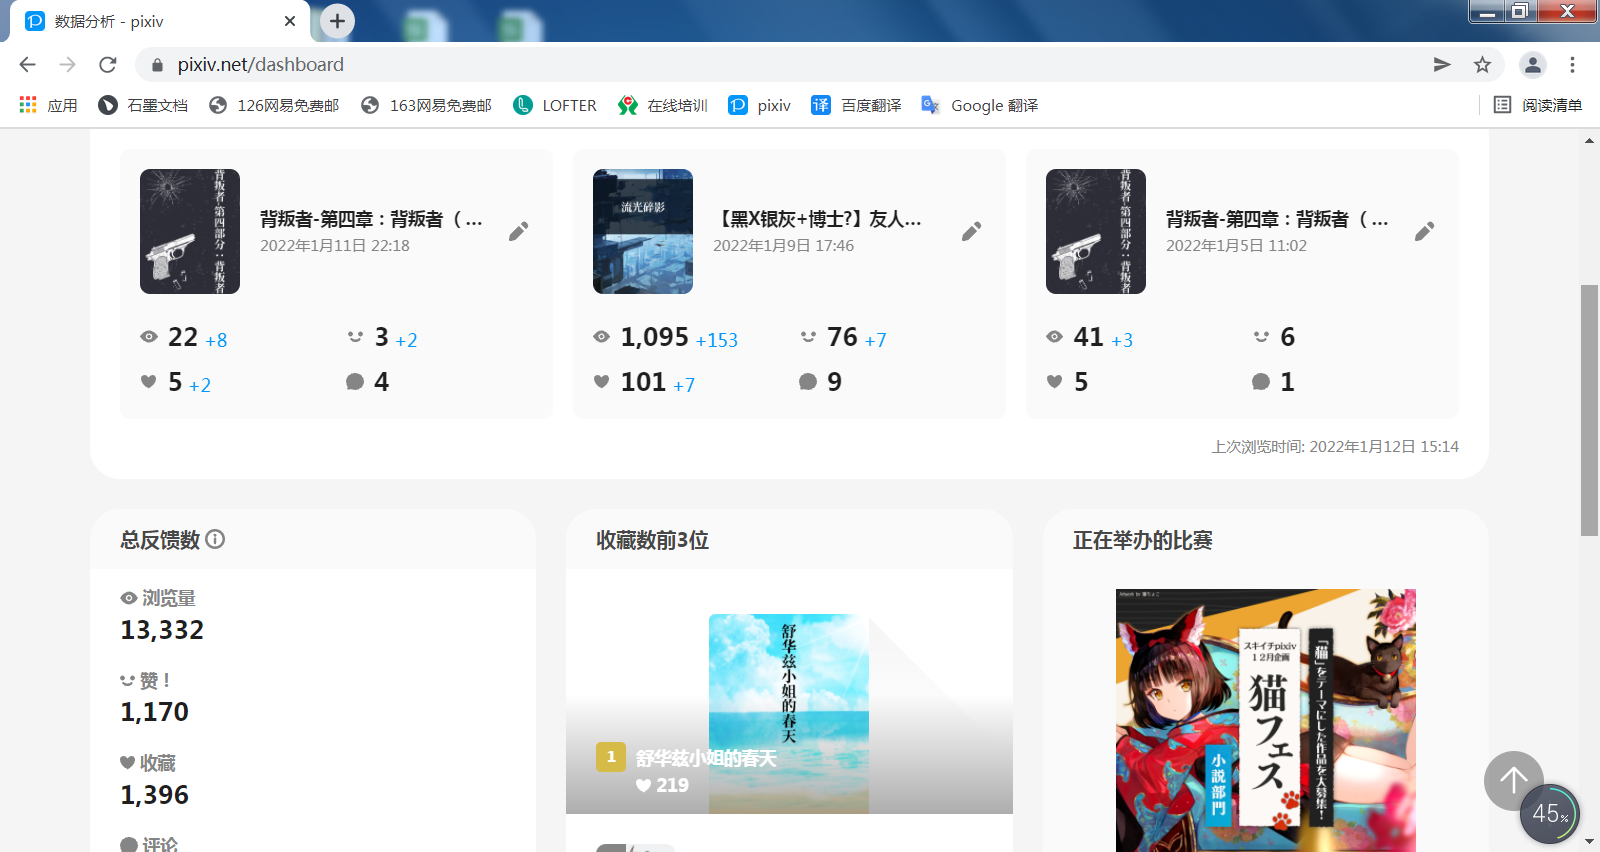
\includegraphics[width=0.7\linewidth]{tei570040063950_ed20dd5e01572ca6287298ecdffa8895.png}
  \caption{作者的Pixiv数据统计图}
  \label{fig:作者的Pixiv数据统计图}
\end{figure}

这点击量和收藏量,高下立判啊……

不想说别的了,赶紧完结这费劲不讨好的玩意去写小黄文吧- -

正文下一页。

\section*{}



战场的另一端——

“安洁,看那个信号弹!”AN94说。几个人抬起头,看到距离不远的地方升起了一颗绿色的信号弹,在夜空中十分醒目。

“是格里芬的信号弹,他们是在指引我们行动的方向!”安洁说。

“可是……那里是红区,安洁。我不认为这是明智的选择。”AK12担忧地说。

“安洁……你恐怕撑不到安全地带。”AN94也说。

“咳……没关系……我愿意再赌一把。”安洁说。

“这可不是靠意志力就能挺过去的事情!”AK12加重了语气说,“仪器显示,这个区域的污染度还在增加,进入红区只会让你的症状更加严重!”

“这座城市里任何地方都有污染,”安洁摇了摇头,“绕开红区吸收的辐射也不会少,除了消耗更多时间外没有其他好处。”

“那就走吧,AK12。感染者增多了,不能拖延下去了。”AN94说道。

“不,我强烈建议绕开红区。”AK12依然反对安洁的决定。

“没时间浪费了!咳咳……”安洁说着剧烈地咳嗽了起来,“AK12,AN94……如果……如果……你们知道……咳……咳咳咳……!咳——!”

“好了,别争了。”一直在旁沉默的陆久开口说道,“安洁的选择是正确的,绕远的话不知道路上会遇到什么,至少格里芬指出的那个方向要相对安全一些。我们必须穿过红区。”

“安洁根本撑不到那时,”AK12说,“她会死在路上的。”

“那就穿上这个。”陆久说着解开防弹衣,然后脱下了自己的防辐射服递给安洁。

“这——”安洁微微睁大了眼睛说道,AK12和AN94也愣住了。

“不要误会。为了让自己活下来,我不会吝惜牺牲你们的。但现在是非常情况。”陆久说,“我没有时间可以浪费,所以必须快点结束这些事情。如果安洁能在辐射中活这么久,那我受点污染,应该也问题不大。所以,就当帮我个忙,快点行动。”

“你这么说,是怕我不肯接受吗?没有必要。”安洁勉强地笑了笑,接过了陆久的防护服,“时间对我来说同样重要。虽说我不忍心为了让自己活下来而牺牲你,但既然是你主动要求,我也就没必要推辞了。”

“呵,请笑纳。”陆久笑了一声说,“不过,这个防护面罩我就自己留着了,我不想让某些人看到我的脸。”

“我能理解。”安洁说着穿上了陆久的防护服,“总之,还是多谢了。这套衣服等穿过红区我就还给你。马上行动吧。”

AK12在最前面开路,AN94背着安洁走在中间,陆久则走在队尾。几个人迅速行动,用了大约四十分钟就抵达了信号弹指示的区域。

“建筑的外墙是辐射最强的地方,请尽量远离。”AN94提醒陆久。

“我知道。不过走在街道中间总是不习惯,有种莫名的危机感。”陆久说。

虽然在无线电静默,但他没有关闭耳机的电源,所以能够听到因为辐射而产生的微弱噪音。在靠近建筑物的时候,噪音会明显增强。

“这是士兵的本能……”安洁用微弱的声音说着,“不靠着掩护物,心里总感觉惴惴不安……我也有这种感觉。不过这里的辐射量,足够让军方忌惮三分……所以应该是安全的……”

“正因为如此,我们要赶紧找到我们的接头人然后离开这里,不然受伤的可是陆先生。”AK12说,“我听说因为骨骼密度的原因,男性会在射线中受到更大的伤害。”

“可是给我们发信号的人到底在哪?”AN94说,“这个地方太大了,没有无线电我们无法准确定位——”

“惊喜!!”AN94话还没说完,残壁的阴影中忽然跳出了一个人影,而且在放肆地大笑着,“啊哈哈哈!终于找到你们啦,忤逆小队!”

陆久立即将枪指向了那个人,但却被AK12伸手将枪口托了起来。

“你要是动作比语言再快一点,我就会把你判定成敌人发动进攻了。”AN94说。

“抱歉,这是AR小队的M4SOPMODII,这边是忤逆小队的AK12和AN94。”阴影中又走出了一个人,用略带歉意的语气说道,“我是HK416,你们两边都见过我。”

“可以的话倒不是特别想见到你,不过现在也没有办法。”AK12说。

“没错,我们可没时间增进感情了,说正题吧——安洁在哪儿,她怎么样了?”416问。

“安洁……她——?”

AK12朝后看了一眼,416随着她的目光望去,发现安洁躺在AN94的背上,却没有了动静。

“没死,刚才还在说话。”AK12说,“可能是因为太过疲倦,昏睡过去了吧。只是后面的战斗暂时只能靠我们了。”

“那只好下一次再打招呼了。”416说,“不过这里不只有我们,格里芬装备了一些重火力人形。”

“嗯,我听帕斯卡说了。”AK12说,“那些家伙靠得住吗?”

“当然,都是我们的新玩具!”SOP2兴奋地说道,“她们可以远程支援我们,是对装甲和集群目标的专家哦,大家绝对会喜欢的!”

“那我们暂时还有救,想想接下来该怎么办吧。”AK12说。

“如果有紧急情况,我们可以进入建筑物内部,那里的污染成都要低得多。虽然无法完全脱险,但是暂时不会对安洁形成致命威胁。”AN94说道。

“还是继续往污染更轻的区域移动吧,安洁这个状态,可能要撑不住了。”416说。

“是啊,我们终究要离开这座城市才行。”AK12说道,“等等,有声音……是军方的人形!冲我们来的!”

“前面有一条弃用的防线,先躲进去!”AN94立即背着安洁奔跑了起来,但眼看着军方的作战机器人已经移动到了可见的距离,并且已经准备好了开火。

“快点!我们到了!”AK12喊道。

“重火力小队,掩护我们!”416也顾不上无线电静默了,打开对讲机大声说道。

……轰!轰!几枚导弹从天而降,火焰覆盖了军方的前线。在重火力的掩护下,几个人顺利冲进了掩体。

“我们还有很多王牌,别担心,就算来几个坦克也一定能对付!”SOP2说道。她的语气很乐观,但陆久知道击溃铁血犹如摧枯拉朽的军方,不可能仅靠几发导弹就能消灭。前来进攻的军方人形很少,只能说明它们是探查情况的侦察兵,大部队一定还在后面。

……呲,呲。416的对讲机里传来了声音,有人在用公共频道发出信息。

“安洁莉娅……你果然没让我失望。”一个男人的声音渐渐清晰地响起,“你从那场爆炸中活了下来,只为了给我一个能亲手杀掉你的机会。”

毫无疑问,说话的是军方的指挥官叶戈尔。

“如果你要找安洁算账的话,恐怕已经晚了。她已经死了。”AK12沉声说道。

“我不这么认为。在现场发回的影像中,我看到你们还背着她。”叶戈尔冷冷地说道,“你们绝不会背着一具尸体到处逃命的。我知道她只是昏过去而已,就像我知道你们会来到这里一样。”

“他算好了通往绿区最快的路线在这里。”416小声说,“我们的行动,早就被他看穿了……”

“我会确保你不会死在炮火中,安洁莉娅,你听到了吗。这样我就能亲手揪出你,为我的部下报仇!”叶戈尔说完,关闭了通讯。

\section*{}

“军方的坦克大概已经在路上了吧。我们该怎么办,马上转移吗?”AK12对着陆久说道,声音里透出了绝望。

“没用的,没有人的双脚能跑过坦克。”陆久说,“我们这次要和他们正面打一仗了。”

“那个人是……?”听到陆久说话,416惊讶地问道。她早就奇怪这个带着面罩的男人是谁,只是之前忙于作战没有来得及问。此时凭声音她已经听出说话的是陆久,只是不敢相信他竟然会出现在这里,而且和安洁在一起。

“我是安洁的同僚。”陆久背对着SOP2取下了面罩,对416使了个眼色。他不想让其他人知道他们认识。

“哦……是这样。我是HK416,是404小队……”416很惊讶居然真的是陆久,但看到陆久的眼色,她勉强掩饰了过去,装模作样地开始了自我介绍。

“知道了,说我们眼下的事情吧。”在416说出露馅的话之前,陆久开口说道,“如果这家伙是来找安洁报仇的,那么他应该是私自行动,带领的兵力不会太多。我们要占据有利位置,依靠重装部队的支援,击退他们。416,重装部队能提供什么样的火力支援?详细说说。”

“重装部队装备了三种武器:40毫米榴弹发射器、82毫米迫击自动炮和反坦克导弹。榴弹发射器的射速很快而且火力覆盖面广,但是对装甲目标效果较差。迫击炮射速要慢一些,但能对轻装甲造成有效毁伤,并且能够发射多种特殊弹头。反坦克导弹是精准的反装甲武器,装填速度很慢而且杀伤范围有限,但能够有效摧毁各种装甲目标和工事。”

“很好,听起来能派上点用场。”陆久说,“听着,现在由我来指挥作战。把我们的通讯器都连线,把你们看到的影像都传过来,搭建起一个简易指挥平台。416用激光引导重装部队,根据我的标记进行攻击。其余三个人负责拦截漏网的敌人。我听说你们都是身怀绝技的特战人形,这次就看你们的本事了。”

“好的。你们两个掩护我,我来对那它们展开电子攻击。”AK12说道,“对方应该全部是作战机器人,我试试能否控制几个。”

“那你呢?”416问陆久。

“我当然是带着安洁去安全的地方隐蔽起来。难道我还要亲自作战?”陆久说。

“说得也是。”416嘀咕了一声,显然觉得这不像是陆久说出来的话。

“都明白了的话就马上去找合适的位置。”陆久说着一把抱起安洁,向着后方一座看起来较为坚固的建筑走去。

走进房间,陆久找了个远离战线的角落把安洁放了下来,然后将自己的计时器摘下来放在地上。这个计时器是陆久身上唯一的高科技玩意,能够支持多种数据链接,并且有投影的功能。他打开投影,几个人看到的画面立即映在了陆久面前的地板上。

“我说……陆司令?”

安洁似乎是醒了,在一旁用微弱的声音说道。

“怎么了?”陆久应了一声但没有回头,目光依然紧盯着面前的影像。

“你把我身上的……防护服脱下来,自己穿上吧。这里的辐射量大……你会受伤的。”

陆久微微侧目瞥了安洁一眼。

“你的伤势很重,更需要这套衣服。”陆久说,“再说外面的战士正在准备战斗,我却在脱你的衣服,我们有这么悠闲吗?”

安洁“噗嗤”一声笑了,虽然声音很虚弱,但陆久能够听到她是在笑。

“没想到陆司令……还挺有幽默感。”安洁说道,“外面情况……如何?”

“格里芬的接应小队到了,重装部队也已就位。但军方的人预计很快就会打过来。我已经部署了防御,依靠重装部队的火力支援,希望能够击退它们。”

“作战成功的可能性高吗?”

“应该还可以……前提是对方的兵力和我预计的差不多。如果叶戈尔找你只是为了报仇,他不太可能调动大规模的部队。”

“你说得很对,他不是军方的最高指挥官……所以这次他很大可能是……私自行动。”安洁说,“不愧是格里芬……首屈一指的指挥官,给人的感觉真可靠啊。”

“你也是会从其他人那里寻求安全感的人吗。”陆久耸了耸肩说,“几个小时前我还以为,你是一个只会自力更生的人呢。”

“哈,几个小时前……乃至十几年中,我也一直这么想的。”安洁说,“但就在那么一瞬间,我感觉自己的观念变了一点……我开始觉得如果能依靠什么人的话……也挺不错。”

“为什么忽然出现这种念头了?”陆久问。

“因为体验了一些……前所未有的经历啊。”

“是什么?”

“你知道吗……我都数不清自己有多少次因伤被撤离战场了。我离开战场时有三成是被扛着、两成是被背着,还有五成是被抬着……但仅有这一次,我是被公主抱着离开的。这让我意识到……我也是个女人这件事,不仅仅是在生理意义上。”

陆久笑了笑。

“如果手里有足够的兵力,我也想说‘我来对付他们’这种逞英雄的话。”陆久说,“可惜敌众我寡,我没有太大的把握让你依靠,实在是不好意思。”

“已经足够了……AK12说得没错,见到你之前我本来……已经打算放弃了,正是因为你的出现,我才又坚持了一阵。”安洁说,“不过,我建议你还是赶紧走吧。离开这里后……你沿着城市的西部边缘绕开原爆点区域,就能到达你的目的地。虽然会花些时间,但路上小心些……就没什么危险……”

“那你呢?”

“我留在这里,吸引敌人的注意力……军方的目标是我而不是你,只要离开我,你就会安全得多。而且说实话……我感觉不太好。我觉得自己这次……挺不过去了。”

“还没到时候。”陆久说,“你只要穿着那套衣服,就能保持稳定的状态,短时间内不会恶化的。”

“何必呢。”安洁说,“帕斯卡拜托你救我,不过是……舍车保帅之举,你不可能看不出来吧。我活下来的可能性太小了……搞不好把你搭进去,最后还是没用。帕斯卡的冒险,承担风险的……是你。你不是,还有自己……要做的事情吗……”

“我知道。但我也是了解风险之后才来的,此刻也是经过认真考虑做出的决定。”陆久看着安洁的眼睛,平静地说,“我认为根据我的计划,有很大概率能够击退敌人并带你离开。所以在战斗依然有效的时候,我不会选择放弃或者逃离。”

“呵呵,我算知道帕斯卡……为什么会看上你了。”安洁虚弱地笑了笑,“我听说她对你动心的时候……还不相信,因为,你懂的……她那种人对男人,已经很难有除了性欲之外的感觉了。但我现在相信了。你真是个,很棒的男人……好到我都忍不住,要对你动心了……”

“过奖了”,陆久笑着说,“也没那么好。”

\section*{}

“让导弹小队摧毁那辆坦克。还有它后面那些轻步兵,用破片榴弹清理掉。快!”

“收到!目标已标记,导弹送出!”

“敌人还在不断袭来!AK12的状态不太好,长时间大量控制军方单位,她的电子战模块已经过载……而军方的安全策略也在不断升级,越来越难以侵入!”

“坚持住,把控制数量降低三分之一。命令迫击炮切断它们的增援,在这几个坐标投放破片弹幕!”

“坐标已标记!但迫击炮小组说弹药已经不多,只剩不到一半……”

“告诉她们打光所有弹药就可以回去了,所以她们最好手快点!你们在下面保持火力压制,SOP2,还能应付吗?”

“小意思!我打得正带劲呢!!来呀、杀呀,啊哈哈哈哈哈……!!”

战场上,枪炮声和呼喊声混成一片,加上时不时有军方的单位被AK12控制,陆久已经分不清敌我目标了。他唯一确知的是敌人的兵力远比他预想的充足,战线只是勉强维持,随时都可能崩溃。

莫非刚才听安洁的话,自己先走一步才是上策?陆久心想。但是现在后悔也已经晚了。安洁已经有一阵没有出声,但是还有呼吸,似乎是昏过去了。

不能再拖了,陆久心想,必须马上撤离这里。

“所有单位,准备转移!”陆久说,“416,通知所有重装火力小组,把她们剩余弹药的一半投向火线位置。”

“一半的弹药?”416以为自己听错了,“火线上敌人没有那么多,我们如果节省一点的话……”

“节省一点只是晚死一会儿,我们现在就需要火力掩护!”陆久打断了416的话,“这是命令、不是请求,给我发射!马上!!”

“……好的,明白!”

重装火力小组收到命令发动了齐射,天空中传来一阵呼啸的声音,接着是剧烈的爆炸。火焰吞没了敌人的战线,为壕沟里的战术少女们制造了短暂的停火间隙。

“我们撤了!动起来,快、快!”

陆久一边喊着一边跳了起来,然后抱起安洁朝着外面奔去,几个战术人形没用片刻就追了上来。

“刚才那一下真过瘾!就像一场大烟花,把它们炸了个稀巴烂,嘭——轰、轰!哈哈!”

SOP2手舞足蹈地描述着前线的火力覆盖,很是兴奋,但其他人都很沉默,因为她们知道眼下的形势并不乐观。

“安洁怎么样了?”AK12问道。

“呼吸和心跳都还有,应该只是昏过去了。”陆久边说边把安洁交给了AN94,“她的意识一直断断续续,身体实在是太虚弱了。”

“再这么来一次,安洁恐怕就撑不住了。”AN94说,“要是有肾上腺素就好了……”

“肾上腺素!你为什么不要面包呢?”416叫了起来,“现在重要的是下一步去哪?!”

“安静,不要慌!”陆久喝道,“这次齐射能让军方好好掂量掂量我们的实力,他们估计要观望一阵才会大规模追击。下个据点的位置安洁告诉我了,在敌人追上来之前赶紧转移,跟我来!”

\section*{}

几个人再次一路急行军,十几分钟后到达了另一个据点。

“这里的辐射量低了许多,”AK12检测了一下这个据点的辐射量,点点头说道,“不过没有防护措施依然会对人体有伤害,所以还是尽量不要留在这里。”

“呼,呼……关闭无线电通讯。”陆久气喘吁吁地说着,“军方应该暂时找不到我们了,但他们迟早会找到这里的,此地依然不宜久留。还有,唤醒安洁。不能让她再昏睡下去了,否则她的体力只会更衰弱。”

“安洁……安洁?”AN94轻轻摇晃着安洁,但她毫无反应。陆久拉出饮用水袋的软管对着安洁的脸,然后一捏水袋,已经冰冷的水喷了她一脸。

“噗……咳、咳咳……”安洁渐渐恢复了意识,“怎么……我……还活着吗?”

“是啊,我们都还活着,至少目前还活着。”AK12说。

“发生了什么?”

“我们击退了军方的进攻,然后转移到了这里。”AK12说,“我们和格里芬的接应碰头了,我想应该是多了一丝希望。”

“安洁——!”见安洁恢复了意识,SOP2兴奋地喊道。

“SOP2?是……你吗?”安洁说。

“是我!没想到吧!”

“你好像变了很多。你是不是用铁血的零件……修补了自己……?”

“抱歉,污染区内干扰严重,我们无法定位你们的频段,只能先赶过来再联络了。”416打断了两个人的寒暄,“毕竟污染一直在不规则地扩散,辐射感染也在加剧,只要我们还在战场上,无论从哪里撞见感染者都不奇怪。”

“HK416……你也在这里?”安洁微微睁大了眼睛。

“很意外吗?”

“404小队的……其他人呢?”

“UMP45受了重伤,其他人为了照顾她先撤离了,抱歉她们来不及向你问候。”

“没关系……安全撤离了就好。不过,虽然你们来了,让我安心很多……但是光靠你们……没法抵挡军方……”

“我们知道,格里芬派遣了重火力单位,通过远程支援帮我们守住了防线。”

“仅仅靠这些还不够,”AN94说,“刚才的战斗已经证明了,我们只能勉强抵挡军方的攻势。而且使用通讯设备虽然可以和外界联系,但也会让军方知道我们的位置。”

“叶戈尔集结了军方全部残余力量来消灭我们,他们一旦确定我们的位置,就会迅速包围我们。”AK12说道,“我们的移动速度不可能快过他们的机械化部队。他们先头的侦查部队也许很快就会找到这里,我们得尽快想办法对应。”

“那不就只有趁现在立刻突围了吗?趁现在包围网还没完成,把拦在前方的敌人全部消灭吧!”SOP2说。

“军方的后续部队马上就会到达,这太冒险了。我认为还是保持低调,避开军方的侦察部队离开这里比较稳妥。”416说。

“没那么容易,敌人的探测设备很先进,很快就会被发现我们。我觉得还是——”

“咳……咳咳!咳咳!安静……”

“安洁!?”AK12惊呼。

“刚才的爆炸波及了安洁,她体内的坍缩液侵蚀得更快了,我们时间不多了!”AN94说道。

“安静!!”安洁用力大声说道。一瞬间,吵闹的人形们都安静了下来。

“陆久,你说……?”安洁喘息着说道。

“……”

房间里的目光齐刷刷地集中在陆久的身上,但陆久没有说话。

“装备、火力、人员数量,所有方面我们都处于绝对劣势。正面战斗,我们没有任何胜利的可能,这是客观情况。”沉默了片刻后,陆久说道,“但我们的目标不是正面的胜利。如果只是撤离,并非毫无希望。”

“可是我们的移动速度……也远不如军方。我们能逃脱吗?”安洁说。

“速度不如敌人的话,就拖住他。”

“对方的兵力……百倍于我们。要如何,延缓他们的速度……?”

“东方的兵书里,有个著名的‘空城计’,善于谋略的军师只在城头弹琴,就能吓退率领数万大军的敌将,他是利用了敌人心理上的弱点。”陆久说道,“战争从来都不只是单纯的兵力比拼,心理战是转换双方优劣局势的关键。这就是所谓的‘兵者,诡道也’。”

“呵,呵呵……”安洁笑了,“对啊,我们还有阴谋诡计……这可是,人类的看家本领……”

“不过,我和军方的指挥官只在影像通讯里见过一次面、说过两句话,我对他几乎一无所知,想设个圈套把他困住,我是做不到的。所以我希望你知道该怎样做,希望你对他有着足够的了解,不然我们这次就死定了。”

“当然,我了解他……东方的兵书里还说,‘知己知彼,百战不殆’,不是吗……我甚至可以说……太了解他了……”安洁喃喃地说着,“但正因为如此,我才感到顾虑,因为我知道……他不是个傻瓜。他会进……我们的圈套吗……?”

“会的。既然他为复仇而来,那就说明他已经被情绪控制了。”陆久说,“他恨你,就利用这一点。让他以为得手了、让他掉以轻心,让他渴望和享受这复仇的快感。然后,在他最得意、最放松的时候,用致命一击将他击溃。”

“我懂了……”安洁说,“我知道,该怎样做了。”

 

同一时间。

军方的无人机已经发现了安洁等人的行踪,通过镜头,叶戈尔在观察着安洁躲藏的地点。

“那个女人逃到那堆建筑里了,她受到了感染,必须要溜到污染更轻的地方才能保命。和她在一起的几个人形不足为患,她现在手上唯一的牌就是那几个重火力单位,但等到我们的主力部队赶到就不堪一击。我想这个时刻差不多该到了。”

“长官,我们刚刚接到报告,重火力部队预计要比你说的集合时间……晚到十五分钟。”叶戈尔身后的一个士官说道。

闻言叶戈尔转过了头。

“十五分钟?为什么要这么久,他们遇到敌人了吗?”叶戈尔说。

“重火力部队在路上遭遇了感染者,他们希望尽量避开战斗,所以正在考虑绕路。”

“我应该说过了,遭遇感染者就全部消灭,让他们尽快赶过来。”

“长官,你应该知道那些感染者的身份。他们是——”

叶戈尔一把抓住部下的衣服,将他揪到了自己面前。

“我比你清楚,下士!”

叶戈尔咬紧牙关,感染的痕迹遍布着脸上,让他的表情更加狰狞扭曲。过了片刻,他松开了手,坐在了一摞物资箱上,深深地吸了口气。

“我很清楚,他们是我的战友、是我的兄弟。”叶戈尔低着头说道,“他们中的很多人和我出生入死了十几年,三战的核弹都没有杀死我们,还有人形……我们曾经从那些真正的杀戮机器手中死里逃生。而今天,他们死在了那个疯女人手上。她为了妨碍我们,引爆了一个坍缩液炸弹。”

叶戈尔抬起头,望着面前的士兵们。

“我知道,战争本当毫无荣誉,也毫无感情。但你们也必须知道,最不想杀死那些感染者的人,就是发出这个命令的人,就是我!我想你们都亲眼看见坍缩液造成的污染了……没错,我坦白地告诉你们,那些兄弟没救了,我们救不了他们。我们现在唯一能做的,只有报仇,慢一分钟,就可能错失一切。现在,下士,需要我亲自跟他们再说一遍吗?”

“不用,长官,他们会马上赶到。”

下士拿出通讯器,说了几句话,通讯器里很快就传来了密集的轰炸声。

 “主力部队就要来了,尽快完成包围网,加强警备,在重火力部队炸平这里之前,绝对不能让她们逃出半步。必须在这个战场里消灭她们,这是唯一的机会。”叶戈尔说着站起了身, “我们兄弟们的灵魂今夜将得到安息……而我们,会向罪魁祸首完成复仇!”

 

“继续前进,没多远了……”

安洁趴在AN94的背上,用微弱的声音说道。她的脸已经没有了血色,苍白得像纸,仿佛随时都可能死去一样。

AK12发现了军方的无人侦察机,但高级别的防护程序让她无法侵入,只能勉强瘫痪掉了它。意识到躲藏的地方已经暴露,陆久已经顾不上让安洁再继续休息了,他决定马上向下一个地点转移。

“你们只能偷偷溜走了吧,一群可耻的老鼠!”通讯器里传来明码的通讯,是叶戈尔在叫嚣,“我们已经完全包围了你们!希望你们不要在炮火中灰飞烟灭,这样我就能亲手枪毙你们了!”

“我们暴露了,军方追上来了!”416惊呼。

“不,他们没有追。他们要用远程炮火打击我们。” 陆久说。

“那不是更糟吗!”

“别说废话,快跑,不要回头!”陆久说,“94背好安洁,其他人向前集中!”

“我们该往哪个方向行动,安洁?”AN94说,“……安洁?喂,安洁——!”

“别喊了,她昏过去了。”陆久说,“看见前面了吗,一点钟方向,最高的那个建筑物,那就是我们的目的地。416,呼叫重装部队发射‘白烟’掩盖我们的来路!”

“可是我们该怎么突破敌人的包围?”

“他们不可能这么快。如果他们真的已经包围了我们,就不会先用炮火覆盖了。AK12,扫描战场,看有没有突破口!”

“……有!有一条没有被封锁的街道!”

“带路!所有人,全速前进,快、快!!”

 

十五分钟后。

“长官,安洁的部队逃出了包围网。”下士向叶戈尔汇报道。

“我五分钟前就看到了。难道你们连几个人形都追不上吗?”叶戈尔皱起了眉头说道。

“我们的追击效率比预想中略低。重火力单位一直对我们进行阻挠,他们还用烟雾弹干扰了我们的视线。”

叶戈尔看了一眼战场上发回的影像,画面里是浓重的烟雾,切换到热成像视野也无济于事,只能看到不断闪烁的红黄光斑。

是白磷弹,叶戈尔心想。这种高温弹药对付软目标和建筑物很有效,但对装甲部队几乎是没有杀伤力的,所以现在已经很少见了。但白磷弹有一个特点,就是冒出浓烟的时候还能发出高热,是干扰热成像仪的绝佳工具。

这群人中间有个不同寻常的家伙,这个人通晓一些冷僻、但在战场上相当有效的把戏。会是何方神圣呢?叶戈尔心想。

“那种火力形成不了太大威胁,让高机动单位先行,及时定位她们的行踪。侦察无人机还没有修好吗?”叶戈尔说。

“还在维修中,现在我们只能通过扫描人形的脉冲信号进行追踪,暂时无法以影像确认情况。不过虽然侦测的距离有限,但她们的移动痕迹完全在我们的掌握之下。另外,长官,安洁逃窜的方向上有一座废弃大楼,不排除她们会进入躲藏的可能。”

“这里还是战场腹地,她们孤立无援,逮到她们只是个时间问题。”叶戈尔说,“进入那个大楼她们就是自绝后路,我会欣赏到她绝望的表情,然后亲手解决她。让地面部队准备!”

 

同一时间,撤离小队正在逃亡中。

“大楼到了!”AK12说道,“上层的辐射很低,我们可以在里面为安洁治疗,同时联系格里芬那边接应撤离。”

“可是军方已经发现我们了。我们会被包围的,到时候就没那么容易离开了。”AN94担忧地说道。

“或者,直接用炮火把大楼轰掉……”SOP2说。

“如果他们想那么做的话,我们已经被炮火炸得粉身碎骨了。”陆久说,“叶戈尔一定是想亲自找安洁复仇。进入大楼的敌人,我推测大概率是人类士兵组成的地面部队。”

“那么我们要进去建立防御吗? ”416问。

“不,无论如何我们都是无法和他们对抗的,以安洁现在的状态也无法继续逃亡了。”陆久说,“我们要躲起来,一边给安洁治疗一边等待时机。”

“军方的侦测设备可以在中近距离探查到人形,但我和AK12可以通过伪装信号来躲过搜查。”AN94说。

“我和HK416能伪装成铁血的识别信号,但没什么用,军方会格杀勿论的吧……”SOP2说。

“是时候分道扬镳了。”陆久说,“安洁已经规划好了撤退路线,416、SOP2,你们一起行动,赶在军方的包围圈成型前把撤退路线清理畅通,如果能吸引一阵军方的注意力更好。AN94和AK12在这里协助安洁。”

“协助安洁干什么?”416不解地说道。

“唱她的空城计。”陆久说。

“我不明白……”

“我也不明白,但我认为安洁已经把剧本准备好了,应该会需要戏班子。如果不是这样,那今天就是她在这个世界上的最后一天了。”

听到陆久的话,几个人互相对视了片刻。

“知道了。”416说,“我和SOP2会清理撤离路线,并设法接应你们。希望你们能够顺利,虽然不知道你们想干什么。”

“一个小时之后如果安洁没有出现,你们就可以放弃任务了。”陆久说,“当然,你们也可以再向格里芬或者帕斯卡请示,那就和我没关系了。”

“……那你呢?”临行前,416看着陆久说道。

“我先留在这里,等安洁醒来再离开。”陆久说,“我会想办法逃命的,因为我不能死在这里,所以别担心。”

“我……”416欲言又止。她不知道该说自己担心还是不担心,正如她不知道这次一别后,还会不会有再见。

“好吧,祝你好运。”416说。

“谢谢。我们现在最需要的,就是好运。”

 \section*{}

“安洁逃到哪了?”叶戈尔问。

“信号显示,安洁和她的部队进入了一个位于黄区的建筑群。她们在一座大楼下面停留了片刻,然后继续向北移动了。”叶戈尔身边的下士说,“那片建筑群前方有我们的一处侦察据点,但对通讯没有响应,因此无法确认这个据点的情况。而装甲部队抵达还需要一些时间。”

“别去想没用的事,我们的士兵会尽职尽责,前提是他们还活着……让追击部队尽快通过目击来确认她们的位置和数目,以及安洁本人,确认她是否躲进那座大楼里面。”

“十分钟前我们已经通过信号扫描过大楼了,没有检测到人形的信号。”

“信号可以被伪装,这次战斗我已经见识过16LAB的能耐了,而且我确实很久没看到安洁的影像了。”

“你怀疑她试图让战术人形吸引我们的注意力,自己伺机逃命?”

“牺牲几个人偶去换自己的命,任何人类都会觉得划算。”

“可是安洁的身体状况,已经没有独自行动的能力了。没有人形的协助,她不可能独自进入大楼。”

“真的是这样吗?”叶戈尔说道,“刚才安洁陷入昏迷的时候,那几个人形的作战和撤离行动依然井然有序、毫无慌乱的迹象,而且效率极高。你觉得那些人偶只是在自律作战吗?”

“这……你是说,安洁的队伍里,还有其他人类的存在?”下士吃惊地说道。

“极有可能,而且是个非常精通作战的指挥官。”叶戈尔说,“再去调查一次,靠近那座大楼进行观察。等待追击部队的确认状况,或者一旦发现楼里有什么动静,任何一种情况,立刻进入大楼!不能放过任何一点可能性,绝对不能让安洁逃脱!”

“是!”

 

同一时间,安洁的藏身处。

“嗯……” 

安洁睁开眼,看到了微弱的光线,是凌晨的天光。如果是在南方,现在应该已经到了破晓时分,但这极北之地的黎明来得很晚,所以外面还很黑。

“你终于醒了。我一直在担心你不会醒过来了。”AN94说。

“看来这次我不用问我是不是还活着了。”安洁说。

“是的,和上次一样,”AK12说,“暂且活着。”

“要是每次醒来都是这样,还不如死了……”安洁说,“希望呢,还有吗?”

“这次的希望,在你身上了。”

安洁微微扭了扭头,看了看自己身边说话的人。坐在她旁边的人正是陆久。

“你还在呢……?”安洁说,“我不是说……把我送到这座楼下,你就可以走了吗?我觉得到这里……已经差不多了。”

“我是想走来着,但你还没告诉我SOG小队的情况,而这两位姑娘又非得确认你死透了才肯离开。”陆久说。

安洁勉强地笑了笑。

“AN94会告诉你……只要你问她。你不走,不会是……舍不得吧?”

“要说舍不得,还真有一点。”陆久说,“这大概是我最后一次和格里芬的人融洽地相处,以后若再见,恐怕就不会得到如此友好的对待了。”

“我听说……你的事情了。不过,严格地说……这里的人,都不算是格里芬的人。所以,这些人你可以相信……至少不会一见面,就请你吃枪子儿。”

“是吗。那可真不辜负一起逃命的难友之情。”

“哈哈……那么现在……外面,是什么情况?”

“HK416和SOP2已经离开半个小时了,她们的任务是在格里芬的协助下确认逃亡路线,并尽量吸引军方的注意力。军方的部队估计用不了多久就会杀过来,我不认为他们会不搜查这座建筑物直接离开。事实上,我对416她们能够吸引军方没有抱什么希望,因为这声东击西的把戏太明显了。所以,我希望我们这样东奔西跑,是因为你还有点其他的对策什么的。”

“是的,当然……我有。不然也不会这么让你们费事把我……带到这么个地方。不过,先给我……喝点水……”

“希望你不介意喝我喝过的水。”

陆久将自己的水袋吸管递到安洁嘴边,安洁吮吸着喝了两口,然后喘了一口气。

“我……需要一些时间。”安洁说。

“每个人都在努力争取时间,但时间不会太多。”陆久说。

“这个计划是个……费工夫的活儿。”安洁说,“听着,这座建筑曾经……是我们秘密储藏弹药的地方。在地下二层,有些爆炸物可以……用来制作简易炸弹……不能把军方报销,但是……炸毁这座大楼绰绰有余。我们要……把那些东西装在一楼、二楼和三楼的承重柱上,然后……把引信串联起来——”

“抱歉打断你,我在附近扫描到军方的信号了,他们正朝我们这边过来!”AK12突然说道。

“试着呼叫一下格里芬,让他们的重装火力部队牵制一下?”AN94说。

“没有地面部队的引导,重装部队发挥不了什么作用。”陆久说,“而且这么做只会让军方意识到我们的意图,之前争取的时间就没意义了。”

“没错,没时间了。必须安装好炸药,不然一切就都完了……”安洁说。

“只能希望他们不会来得那么快了。”陆久说,“我在这里照看安洁,你们两个马上行动!”



\chapter{背叛者(十二)}

\section*{前言}


黎明将至,这一场持续了整夜的猫鼠游戏就要结束了。用兵和攻心,陆久已经竭尽全力,却依然难保安洁是死是活。

不过,无论这一场插曲如何落幕,陆久却已不在其中,因为他还有其他的事情要做。

\lineseparator


诸葛亮能在城楼上吓退敌人大军,但叶戈尔不是司马懿,没有亲眼看到安洁断气他是不会罢休的。但这也正是安洁计谋的一部分。而这一计的成功,还需要许多人的配合,天时地利人和,可谓缺一不可。

在太阳升起之前,所有的斗智斗勇将会迎来最终的结局,但陆久却决定和安洁就此诀别——他要先行离开,因为他还有必须要做的事情,没有时间看完这场戏的落幕了。

陆久绕了远路,但是他做出了正确的选择,因为安洁的生死也在间接上决定了陆久的生死。只是这一件事,是陆久很久之后才知道的。

正文在下一页。

\section*{}



与此同时,416和SOP2一边。

在离开安洁等人四十分钟后,416和SOP2来到了一座废弃的军方侦查哨站。这座哨站位于城市的边缘,位置很好,俯瞰着城市外围的荒野。荒野尽出是茂密森林,一旦进入森林,敌人就很难再追击了。

但这毕竟是军方的据点,设计上有着相当的防护水平,想要摧毁它不是一件容易的事。

“根据安洁指出的路线,这个敌方的侦察据点将会是主要阻碍。必须将这里的敌人全部肃清,才能确保安洁的撤退路线。时间紧迫,军方的主力随时会追上来,我们得尽快搞定这件事。”416说。

“可是……这座哨站看起来很坚固。虽然不知道里面还有没有人,但是外围的自动防御系统好像还在运作呢。”SOP2说,“要是AK12在就好了,她能用意念摧毁这些自动武器,说不定还能探查一下哨站里有没有敌人。”

“没有那么现成的事情,而且安洁那边更需要AK12她们。”416叹了口气说,“呼叫格里芬的远程火力支援吧。先打掉防御系统,我们再进去清理。”

416标记了哨站的防御设备,几枚导弹从天而降,摧毁了那些轻型自动武器。

“外围防御已经摧毁,快点用爆破榴弹攻击窗户啊?”SOP2说道,“我们已经暴露了,你还在等什么!”

“等一等。”416说,“我能扫描到一些生物信号,在屋子里。”

“那应该是感染者吧,活人都是些没有武装的后勤人员啊,剩下的不是被感染者干掉了就是逃跑了。”

“不要掉以轻心,确保一个敌人都不能留下,不管那是谁……就在这个门后面。”

两个人靠近医疗室前,里面传来低吟和爬动的声音。

“房间里确实有人,但是根据站位判断,不像是警戒中的敌人……”SOP2压低声音说道。

“也有可能是感染者。”416悄声说。

“总之,我们不能进攻手无寸铁的人类!”SOP2说。

“那不是你能决定的,祈祷我们的视觉反射比扣扳机的指头要快吧。”416说,“准备好,三个数后开始进攻,3、2、1……”

砰!HK416一脚踹开了门,迎接她们的却是一阵恐怖的嘶吼。

“呃啊啊啊啊啊!”

“是感染者!开火、开火!”

一阵杂乱的枪声过后,屋子里沉寂了下来。 

“我就知道……”416低声说道。

“416,角落里……”SOP2说。

HK416看向房间的角落,几个人类正蜷缩着身体,满脸恐惧。

“求求你……别杀我……”看清了来人,一个女人终于呜咽着说,“我只是个医生……求求你们……咳咳……”

“416,那个人被感染了,不过比较轻。”SOP轻声说。

“我……咳咳……只是在救他们……咳……”女人旁边,另一个受伤的男人说道。

 “你们谁也救不了。SOP2,把他们绑起来。”416说着打开了通讯器,“指挥官,我是HK416。我们已经肃清了军方的哨站,安洁撤离的路线上已经没有阻碍了。什么?……好的……我知道了。”

“安洁已经暴露了。”切断通讯,416对SOP2说道,“军方来势汹汹,格里芬方面希望我们能协助安洁。”

“这怎么可能,他们明明伪装了信号……”SOP不可思议地说道。

“叶戈尔的人之前大概是没有看到我们,也有可能识破了我们的计划。虽然军方现在一定已经注意到我们了,但无论如何他们都不会放弃搜查那座大楼的。” 416说。

“我们该怎么办?”SOP2说,“如果军方进了大楼,那我们就白跑一趟了,而且还赶不回去……”

“军方的侦察队还没有进入大楼,他们在追击的同时,一定也在远程观察我们,想通过目击来确认安洁是不是在他们的追击目标中。”416说,“我们得想个办法吸引他们的注意力,让他们认为安洁在我们这边。”

“这怎么可能?”SOP2说,“我们又没办法变出一个安洁来!”

该怎么办呢,416在心中自问。她感到一筹莫展,因为她对策略这种事情一窍不通。45倒是经常靠耍些危险的花招来获取优势,但那对416来说太难了,更何况是要迷惑人类。

人类的办法……。如果现在换作是陆久,他会怎么办?416思索着。之前他说过的,心理战术……欺骗……

416向着房间的角落看去,在那边,SOP2正在搜罗着可能会有用的药品。当416的目光落在那几个人类身上时,她忽然冒出了一个想法。

“变出个安洁来”吗,416心想。不知道这有没有用……但值得一试。

“SOP2!把那个女人带过来。”416对SOP2说道。

“你要干什么?”SOP把药品塞进背包,惊讶地说道,“我们……不能攻击没有武装的人类!”

“不,我们能。我们是非法人形,不受那可笑的三定律的约束。”416说,“而且我们也不是要攻击她,只是要她稍微配合一下。”

 

军方的指挥部。

“长官,我们的部队目击到了疑似安洁的身影!”下士说。

“什么!”叶戈尔说道。

“但是距离太远了,我们能所见的形象有些模糊。”

“身形是很像,还能进一步确认了吗?”

“通过热成像系统可以确认是人类,她似乎处于昏迷之中,被两名战术人形背着,这两名人形是安洁的部队成员。她们正在朝城市边缘逃窜,预计很快将进入森林。格里芬主力梯队也在兜圈,看起来是在往回撤了。”

“安洁的身体一定是在黄区中恶化了,所以她想拿格里芬的主力当诱饵,然后悄悄逃走。追上去,绝不能让她们逃进森林!”

“收到,那么那座废弃大楼的侦察部队呢?”

“让侦查部队继续监视,然后从主力中分出一支梯队包围那座大楼,严防死守。在确认安洁的身份前,不能掉以轻心。”

这是万无一失的策略吗,叶戈尔心想。主力在追击疑似安洁的人类,格里芬的人形部队也在被严密追踪。就算安洁躲在大楼里,只要她想逃出去,也能第一时间控制住她。

没有别的可能,她没有任何翻盘的办法。那个女人,已经插翅难逃了。

叶戈尔坐在一个空的补给箱上,感觉有些怅然。这场追猎马上就要落幕,但他的心情反而平静了下来。

复仇的滋味是甜美的……但甜美的只有短暂的一瞬,而回味则是悠长的苦涩。这样的复仇真的有意义吗,叶戈尔心想。死去的人,终究不能复生,在这场追猎中反而增加了更多的伤者。这代价是值得的吗?

叶戈尔闭上眼睛,那些曾经的战友的面容在他眼前闪过。

若非这该死的战争,他们都是些普通的人、都是些和善的好人。而当他们走上战场时,却又是那么勇敢和忠诚。可这些优秀的人,只在一眨眼的功夫就都没了,有的甚至变成了可怕的怪物。

兄弟们……

可惜,你们没能看到这场战斗的结束,叶戈尔心想。

不过,就算这场战斗结束了,还会有下一场、下下场,战争是永远不会结束的。所以总有一天我们会再见……也许,那天已经没多远了。

叶戈尔睁开眼睛,咬紧了牙关——

但在那之前,必须让那个女人血债血偿。

“我是自己人!不要开枪——!”

通讯器里传来了吵闹和尖叫吸引了叶戈尔的注意,那是个人类女性的声音:

“咳咳……求求你们!我是被迫的!我什么都没做!天啊——!”

“怎么了?”叶戈尔问道。

“长官,我们抓住了疑似安洁的目标。”他身边的下士回答道,“经确认,对方是我们的医疗人员,被简单化妆成了安洁的样子。那两个挟持她的格里芬人形已经不见了。”

“是那个人形把我打昏丢在这里的。咳咳——我需要……咳咳咳!求求你们……”通讯器里的女人依然在叫嚷着。叶戈尔没有说话。

“她受到了感染,需要治疗,我们怎么办……长官?”

“把她带回来,在路上给她治疗。”叶戈尔沉声说道,然后靠在一辆坦克上,用手指狠狠揉了揉眼眶。

“安洁在大楼里……”叶戈尔咬牙切齿地说着,“她只是在拖延时间,给自己治疗!妈的!”

他在坦克上狠狠地砸了一拳,然后起身走向指挥室。

“长官!我们发现刚才的格里芬小队了,她们正在往大楼的方向移动!”下士说。

“她们在回防,为了保护安洁而做最后的挣扎。”叶戈尔说,“侦察部队呢?能赶在格里芬之前进入大楼吗?”

“可以,但是格里芬支援单位的火力现在能覆盖到大楼,贸然接近可能会遭到攻击!”

“那就原地警戒。所有战斗人员听令,立即前往目标大楼,将其包围!安洁……你耍了多少花招都是白费功夫,你们就算回到大楼,也只是送死。这一次,你绝对不可能逃走了!!”

\section*{}

“跟我说说把,陆久。你那位……‘朋友’的事情。”安洁说道。

AK12和AN94去部署爆炸物,大厦的露台上只剩下陆久和安洁两个人。东方已经有了一丝亮光,但天空中还是群星璀璨,是一场晴夜的景观。

如果这不是在战场之上,此刻面前的也算是好风景,陆久心想。

“你得保持体力,少说点话。”陆久说。

“我得想点什么,不然……我可能马上就会再昏过去,也许永远都……不会醒了。”安洁说,“这里又没有别人,我只能……和你聊天了……”

“我们有什么好聊的。”陆久无奈地笑了笑,“运气好的话,大概再用不了一小时,就该各走各的路了,运气不好,就要就此永别了。”

“那不是很好吗,我们此刻……是可以互诉心声的‘安全倾诉对象’。”安洁说,“我非常好奇你在做的事情,特别是……在对你稍微有所了解之后。你为什么要……冒着丢掉小命的危险,去找那个人形?”

“她对我来说很重要。”陆久说。

“嘛啊,当然了,比命还重要……这我知道。我想知道的是理由。你们之间……发生过什么?”

“发生过许多事情。你大概知道,我……是个囚犯,被再社会化改造之后成为了格里芬的指挥官——格里芬为此花了一大笔钱。而那个人形,是我在这个新世界遇到的第一个战友,也是我后来在格里芬供职时的副官。这次行动中,她被委任了些有去无回的任务,被当做弃子丢在了战场。所以我要去救她。”

“理由很正当,简直有点正当过度了,以至于有些俗套……你们只是普通的战友关系吗?没有别的?”

“你也很喜欢探寻别人的私事啊?”陆久说。

“呵呵,女人嘛,都会有这方面的兴趣。不过可千万不要让其他人知道这件事。”

陆久看了安洁一眼,他发现安洁精神了一些,而且说话不再是一句三喘了。这起死回生的奇效,让陆久暂时止住了结束这个话题的念头。

“你还想有什么别的?”陆久说。

“也没什么……就是指挥官和人形副官之间那种常见的事情,你懂我在说什么。在格里芬,这种事情也不算少见吧?”

“是啊,我们……也有那样的事情。”陆久说。这中间的事情实在是太复杂了,说到中午也说不清,所以他决定从客观上承认安洁所说的这个“也没什么”。

“但不只是那样?”

“也许不只。”

“你对她有感情。”

“嗯。”

“你……莫非是爱上她了?”

“是啊,没错。”

陆久看向安洁,稍稍皱起了眉头。他不喜欢别人关注自己的私事,虽然这事情确实有点有违世俗,但那是他的自由和权力。不过陆久在安洁的脸上没看到任何鄙夷的神色,安洁看起来只是有些惊讶。

“怎么了?”陆久说。

“没什么。我是吃惊你竟然这么坦白地承认了。”安洁说,“说实话,我觉得……嗯,很美好,那个词怎么说来着?有点浪漫,没错。一同战斗的战友,终于变成了相互爱恋的伴侣,这是多么理想主义的——唉,不过帕斯卡要是知道自己的魅力输给了一个人形,她恐怕会非常的,嗯……”

安洁陷入了沉思,陆久可以确定她现在的思维一定非常活跃,因为根据陆久的经验,揣摩帕斯卡的想法无疑是一件重脑力劳动。陆久莫名地有些欣慰,因为可以结束情感话题是他喜闻乐见的,可惜他的欢喜只持续了不到一分钟——

“军方的人来了。他们正在对我们展开包围。”陆久说。从露台上他已经能够看到大楼周围正在交替移动的士兵。

“还真快啊。这一点时间,根本不够部署有效数量的爆炸物。”安洁说。

“安洁!军方的人来了,他们正在准备进攻!”呼叫器里传来了AK12的呼声,她已经顾不上继续无线电静默了。

“爆炸物怎么样了?”安洁说道。

“一楼安放了一半,二楼三楼完全是空白!”

“在所有剩下的预定位置安放起爆引信。只安放引信、不装炸药,做完后马上来我这里。快!”

“只装引信?那岂不是没有任何威力……啊,好吧!”

AK12知道没时间细问了,结束通讯迅速开始执行安洁的命令。

“军方已经开始行动,就算是只放引信,也没时间了。”陆久说。

“唉,那就放多少算多少吧。”安洁叹了口气,“其他就看命了。”

“这样有用吗?”

“我不知道。兵书上从没有万全之策,只当临死的最后一搏吧。”

“还需要多长时间。”

“二十分钟?快点的话,也许十五分钟。”

陆久看了安洁一阵。

“我去会一会下面的先生们,尽量拖延一点时间。”陆久说着拿起了他的自动步枪,“如果我没死的话,就直接去我要去的地方了。所以就此别过吧。”

“这个还给你,无论成功与否,我都用不到了。”安洁挣扎着坐起身,脱下了自己身上的防护服,“战场的详细地图资料我已经传到你的‘手表’里,但多数情报可能已经变化,所以只做参考。”

“我会先行确认的。”,陆久接过防护服迅速穿好,点了点头说道,“那么,我走了。愿命运垂青于你。”

“你也是。”

\section*{}

陆久还没走到二楼,就听到了一片杂乱的枪声。密集的枪声是军方在开火,而偶尔响起几声的,则是AN94在还击。为了争取时间,她用正面交火来吸引军方的注意力,而AK12则去独自安放爆炸物了。

AN94的火力远不敌军方,但她找到了一个很好的位置,在狭窄的楼梯中居高临下,暂时牵制住了军方。

“情况怎样?”陆久来到AN94身边说道。AN94已经负伤了,殷红的血液染红了她的浅色头发,但她依然坚守在最有利的位置没有后退。

“敌人都是人类士兵,大概是因为知道AK12能控制他们的人形。”AN94边开火边说道,“他们的数量和火力都有限,但是我的火力太弱了,恐怕坚持不了多久。”

“明白了。”陆久点了点头说,“我来守住这里,你赶紧去帮AK12,然后去安洁那边。她已经体力不支,身边不能没有人。”

“可是,您一个人对抗这么多士兵……”

“我不会直接和他们交火的。我要和他们谈谈,争取用‘和平’的方式解决问题。”

AN94迟疑地看了陆久一眼,然后点了点头,离开了。看着AN94走远,陆久对着楼道里喊道:

“别开枪,我不是战术人形。停火!”

枪声真的停了,因为楼下的人们没想到竟然还能听到人类说话。

“让你们的指挥官出来,在楼道口就好。我要和他谈谈。”

“我就在这里!你是什么人?表明身份!”陆久立即听到了回答,敌人的指挥官就在士兵中间。这让陆久确信了自己的猜想,这群士兵的带头人正是叶戈尔。

“我曾经是格里芬的指挥员,但现在已经不是他们的人了。我想要向你提一个对我们都有好处的建议!”陆久说。

“……是你。我记得你的声音。”叶戈尔说,“你不是什么指挥员,而是北方军团的总指挥官。你叫陆久,对吧?”

“正是鄙人。我也知道你是叶戈尔阁下,别来无恙?”

“托你们这些狗杂种的福,还没被干掉。你是有什么遗言想要交代吗?”

“不,我和你交涉是为了活下去。我的要求很简单,放我走,然后你就可以大摇大摆地去找安洁算账了。我保证不会再有任何抵抗!”

“可笑,你已经到了穷途末路,插翅也难飞了。我抓到安洁是迟早的事情,为什么要饶你的狗命?”

“那我不得不告诉你一个不幸的消息,安洁已经受了严重的辐射伤害,现在只剩下半条命了。我知道自己敌不过你们所有人,但我在这里周旋半小时是轻而易举的。到时候你就算杀上来,也只能看到安洁没有气息的尸体了。这就是你渴望的复仇吗?”

“这么说,你是要出卖安洁来换取自己活命了?没想到格里芬的军区司令,也是个出卖战友的渣滓!走狗永远是走狗,无耻的鼠辈!”

“你错了,叶戈尔。安洁不是我的战友。格里芬为了救出AR小队,派我的人去牵制你们,然后又被他们抛弃在辐射区,相信这件事你该有点印象。我是要去救我的人,只是被安洁裹挟着才帮她撤离。我和你之间没有任何仇恨,而且我现在是格里芬的通缉犯,不可能再回格里芬,我们没有理由相互为敌。安洁已经没有撤离的可能了,如果她现在活着唯一的价值就是实现你的复仇,我甚至对此表示欢迎。我只希望我们能够互不干扰,各自去做各自的事情,因为我们的时间都不多,不是吗。”

叶戈尔没有说话,似乎是在设法证实陆久的话。过了一阵,叶戈尔才说道:“格里芬的军区司令竟然会成了头号通缉犯?你一定是在耍什么诡计!”

“你已经亲自查证还是不相信吗?”陆久说,“在克鲁格被军方拘捕之前我就被宣布为叛徒了,难道你认为这一切,只是为了营救安洁这种可笑的蠢事吗?好好想想吧,我说的句句是真!我只是想自己离开,并不是要带走什么,而且安洁的命可能只剩下几十分钟了!你仔细考虑考虑吧!”

“好吧,你放下武器,我可以保证你的安全。”考虑了片刻后,叶戈尔说道。

“哈,都是战场上混的,你认为我会相信你的话,还是手里的武器?”陆久笑道,“我不会放下武器的,叶戈尔。让你的人离开楼道,我自己下去。不许用武器指着我,不然我会顽抗到底的。”

“……好!你出来吧,快点!”

陆久举起枪,散步一般慢悠悠地走出了大楼。大楼门口有二三十个全副武装的士兵,但正如叶戈尔承诺的一样,他们的枪口都朝向天空,没有指向陆久。而站在那群士兵中间的,正是叶戈尔本人。

见陆久走出来,叶戈尔比划了个手势,那群士兵立即冲进了楼道,大楼外面只剩下叶戈尔和陆久两个人。

“你胆子之大,不仅让我吃惊,甚至让我稍稍有些钦佩。”叶戈尔说,“你就不怕一出来,就被我乱枪打死?”

“我们向来无仇无怨,甚至还做过几天的友军,你为什么要把我乱枪打死?”陆久笑了。

“和安洁一伙的人,死一个就少一个!”

“我说过,我只是受她裹挟才帮她一把,我对她本没什么好感、更不是和她一伙的。现在我已经和格里芬一拍两散,你和安洁之间的事情,我既不想知道、也不想管。如果你不打算阻拦我,那我就要去找我的人了。她们被困在原爆点附近,听说那里已经是真正的地狱了。”说着,陆久拉下了自己的面罩。

“我看了你的资料,你也算是不简单了,三战前入伍,还能活到现在的人已经不多。虽然我始终怀疑你在搞什么诡计,但出于对老兵的敬意,我姑且放你一马。你如果敢暗中坏我的事情,那么就和安洁一样,迟早我会找你算账。”

“呵。”陆久笑了一声,“这个世界我都懒得搭理,哪有闲情管你的事情。不过看在你也是条硬汉的份上,我也赠你一言。试问,为了胜利,你愿付出多少代价?”

“任何代价,哪怕是血流成河。”叶戈尔扬起下巴答道。

“那为了复仇呢。”

“你说呢?”叶戈尔看着陆久冷冷地说。

“为了胜利可以不计代价,这一点我赞同,但为了复仇就不同了。”陆久说,“血债自当血来偿,但为给牺牲的人复仇而让更多的人牺牲,事后就会发现并不值得。好好想想吧!”

说完,陆久把枪背在肩上,阔步向着大楼的北方走去。

看着陆久离去的背影,叶戈尔眯起了眼睛。有趣的家伙,叶戈尔心想,他仿佛能看穿自己的心思一般。毫无疑问,这也是个危险的人,如果今天不除掉他,他日必成后患。

想到这里,叶戈尔抬起了手里的枪。但在枪口对准陆久之前,他还是放下了枪,因为他总觉得陆久在看着他——他不能确定如果向陆久开枪会怎样,但有一点他是确定的,那就是他没空和陆久缠斗。此刻他复仇的对象只有一个,他必须分秒必争。

\section*{}

(陆久离开了,这一节的剧情只和安洁有关,已经没有陆久的戏份,也就是说和背叛者一文的剧情几乎没有联系,所以一开始没打算不发了。

不过想了想还是发出来好。虽然关于安洁后面的故事大家都已经知道了,但总觉得交代一下这一部分,这部分的剧情才算完整。)

\section*{}

叶戈尔的部队占领了一楼二楼和三楼,果真如陆久所言,他们再也没有遭到任何抵抗。

“我们探测到生命特征了,但是很微弱,就在楼上。”一个军士对叶戈尔说道,“另外还有两个人形,在楼顶,距离这里很远。”

叶戈尔点了点头。

“在这里待命。”他说,“我自己去会会她。”

“你一个人去?这是不是太危险了……”

“如果有危险,恐怕也不在上面。我要你们时刻留意四周、大楼外面还有楼顶上的人形,一有情况立刻汇报。安洁是在挑衅,这十有八九是个陷阱。”

“是,长官。”

“安洁,你真的是在坐以待毙吗?不,不可能。”叶戈尔自言自语地说道,“那就让我看看,你死到临头,还能耍什么花招……”

叶戈尔走上楼梯,终于,他见到了那个让他“日思夜想”的女人。空旷的大厅里没有任何遮蔽物,安洁坐在置于正中间的椅子上,仿佛在开一场展览会。不过叶戈尔能够看出她只是勉强支撑着身体,再过一阵她可能就要倒下去了。

“……安洁莉娅。”叶戈尔说。

“你好,叶戈尔上尉。我们又见面了。”

“怎么,你的部下,没有和你在一起吗?”

“你不也一样吗?”

“不,我和你不一样。我的人依然对我无比忠诚,而你已经众叛亲离。你大概没想到,正是那个陆久让我上来的吧?”

“我根本没有想他的事,那家伙本来和我就不是一伙的。虽然我倒是希望他能和你打一架,再为我拖延点时间,不过无所谓,我已经利用了他的全部价值了。你忠诚的士兵们在哪?”

“不用费心套我的话了。对付你,只要我一个人就够了。”

“真会说大话。”安洁勉强挤出一个笑容,“你带着那么大一批人马,大张旗鼓地跟在我屁股后面,现在又成了孤胆英雄?用这种方式追求女人,未免也太难看了。”

“这就是你最后想说的话?比我想象中还要乏味,安洁,我对你的遗言感到失望。”

“抱歉,我就是个乏味的女人。难道说,你还打算在杀死我之前长篇大论一番吗?”

“我看起来像是那种三流电影里的反派吗?”

“我看你的脸很像,而且我知道,你现在的意识已经没那么清晰了。坍缩液影响的不只有肉体,你一边忍着辐射变异对精神的侵蚀,一边被我耍得团团转,现在一定快疯掉了吧?”

“确实,我和我的部下之前表现的确实有些失控,因为我们在那场爆炸之后,就只有一个念头,就是亲手杀了你。你操纵格里芬的人偶表演的那些把戏,不会打消我们半点复仇的渴望,因为我们只有这一个念头,就是见证你的死亡。现在,你的时候到了——去死吧!”

叶戈尔拔出了枪,但同时——

他注意到,安洁藏在背后的手,有所动作。

“呵。真是熟练的拔枪动作。要不是你是敌人,也许我就迷上你了。”

安洁笑着说道,放到了前面的手里,有一件东西。叶戈尔直勾勾地盯着安洁,搭在扳机上的手指终于没有扣下去。

“但是你为什么不开枪?如果我没猜错的话,我想你害怕的是不是这个?”安洁笑着说,她手里的是一个起爆装置,“一时冲动就跑进了这个大楼,你也不想想,为什么我要继续留在这座楼里?”

这时,叶戈尔也收到了楼下传来的通讯。

“长官,我们发现了大楼中埋藏多个爆炸装置!我们目前只搜索了一楼,但是根据扫描到的信号,二楼和三楼还有更多!”

听到部下的报告,叶戈尔的脸色阴沉了下来。

“终于意识到了我的计划?哈哈哈哈。”安洁笑了起来,“没错,我伪装自己让你以为我非常虚弱,然后诱骗你们围住了这个大楼,让人形在承重结构上埋下炸弹,然后就等着你像个蠢货一样冲进大楼。我就是要把你们一网打尽,为了报复你当初背叛我的罪行!”

“安洁……!”叶戈尔咬牙切齿地说道。

“别用那样食肉饮血的眼神看着我,我劝你的手放松一些,如果你开枪打死我,我的人形会立即启动备用的引爆装置。”

“你以为你能威胁我!?”

“我当然可以。我要向你坦白你一件事,这座大楼埋藏的不单单是普通的炸弹,我还混进了坍缩液容器。一旦引爆,你那些外围的部队也无法幸免于难。怎么样?”

“……坍缩液?最后一刻还想耍我吗?别胡扯了,你根本做不到!”

“我为什么会做不到?”

“你在撒谎,不可能还有坍缩液容器!你从哪里弄来到这么多?”

“哈哈,为什么不可能?就因为我之前用过一次?一个没用过核弹的人和一个用过一次核弹的人,你更相信谁会按下下一次的发射按钮呢?不如问问你的手下,他们现在一定在忙着找我们埋下的小礼物吧?”

叶戈尔一只手继续瞄准了安洁,一只手打开了通讯器。

“这幢楼里,能否探测到高浓度坍缩液反应?”叶戈尔说。

“敌人的话刚才我们听到了,已经在搜索了。但是周围坍塌辐射污染太严重,无法进行定位。”

“怎么样,现在相信了么?”安洁说。

“既然如此,你还在等什么,就如你计划地那样按下按钮啊!!”叶戈尔咆哮道。

“哈哈,咳……哈哈哈……”

“你笑什么!?”

“我笑你明明自己已经快要崩溃,还有工夫想着给别人施加压力。好吧,告诉你一个好消息,你今天的运气非常好,因为你还有另一个选择。命令你你包围大楼的部队撤到城区外,让我还有我所有的人形离开这里,也许我可以考虑放过你们。”

“你想得太美了,安洁!好不容易走到这一步,我不可能让你逃掉!有本事你就按下按钮和我们同归于尽啊!”叶戈尔怒气冲天地说。

“不要得寸进尺!这是你最后的机会了!”安洁不知从哪来了力气,厉声说道,“不然你就再经历一次辐射吧!但这一次,你和你部下全部都别想活下来!”

“你以为我会害怕死在这里?我们是军人,安洁,你了解军人!”

“我了解,叶戈尔,但你是他们的长官!人形在你眼里毫无价值,但人类呢?他们是你的战友和兄弟,你会为了你的复仇,让死里逃生的他们再一次被卷进地狱吗?”

“我的部下……他们不会畏惧牺牲!”

“你还想再让你的部下们死在脏弹之下吗!你太自私了!想想他们的未来、想想他们的家人!只要我按下起爆器,这次你,还有任何人,都不会再有复仇的机会了!”

“你是在虚张声势!不然你就是疯了!!”

“是的,我就是疯了!!所以我现在什么都干得出来!因为在所有人都抛弃我之后,这就是我最后的救命稻草!我告诉你,现在我什么都不怕了!用我和几个不值钱的人形来抹杀掉这么多敌人,对我来说简直赚翻了!无论你做了什么,对我来说都是胜利,所以……快点决定吧,要么我们都能活下去,要么让你和你的部下一起为我陪葬!!”

安洁狰狞地笑了,叶戈尔看到她的眼中没有任何多余的渴望,她只想做一件事——看着他在逼迫之下做出选择。

但叶戈尔知道,走到这一步,他其实已经没有选择了。

“这次你赢了,安洁。”叶戈尔说着慢慢放下了枪,“暂时,赢回了自己的狗命。”

“全体人员注意!”叶戈尔对着通讯器说道,“大楼中有疑似混有坍缩液的爆炸物,所有人撤退到3公里外的安全距离区域。这是命令,立即行动!”

安洁站了起来,摇晃着一步步走向了窗边。她看到外面的部队正在全线撤离,她的撤离路线已经没有阻碍了。于是她拿出了通讯器。”

“来接我。”安洁对着通讯器说道,然后再次转向叶戈尔,“作为军官来说,你是一个好上司。我承认你是个合格的军人,但你站在了错误的队伍里。”

随着一根绳索坠下, AK12和AN94同时从窗边跳了进来,举枪朝向叶戈尔。

“所以,现在你要铲除了我了么。”叶戈尔冷笑着说道。

“不,杀了你对我没什么好处。铁血的主脑已经跑了,我们有非要杀死对方的理由吗?”

“你知道我有。”

“我也有杀死你一万次的理由,叶戈尔。但不是现在。我还有事情要做。”

“事情不会这么结束的,安洁莉娅……我们走着瞧。”

在叶戈尔犹如火焰的仇恨目光注视下,安洁被AK12背在了肩上。

“下次的事,等到下次再说吧。”安洁说,“这个小礼物就留给你做个纪念,希望能给你留下一个值得反思的教训。”

安洁把起爆器扔在地上,在同一瞬间,AK12和AN94带着她跳下了窗户。叶戈尔慢慢走向窗边,捡起了那个起爆器,沉默地看着已经撤离得空无一人的窗外。

半个小时后,气喘吁吁的拆弹小队队长来到了叶戈尔面前。

“长官,我们已经排查了所有三层楼房,安放在大楼的绝大多数炸弹……只有发出信号的引信,没有装炸药。无人机仔细扫描了整座大楼,也没有发现带有高浓度坍缩液的容器。”

“呵呵。”叶戈尔冷笑了一声,他想起陆久对他说的话。

为给牺牲的人复仇而让更多的人牺牲,是不值得的。这到底是规劝,还是暗示?叶戈尔也无法确定。但他觉得这句话确实没错。 

“长官……?”

“知道。我知道。”叶戈尔看着安洁留下的起爆器,脸上的表情平静无比,“我早猜到这是她的虚张声势,有99.99\%的可能是这种结果……但我没有选择。你们知道,那个女人是个疯子,她什么都能做出来。只要有万分之一的可能,我就不能拿所有人的生命去冒险。”

“长官……下一次,无论发生什么,只要有你的命令,我们随时做好了牺牲的准备。”拆弹小队的队长说道。

一丝晨光从大楼残壁的缝隙里照了进来,虽然城市几乎已经化作废墟,但太阳依然如常升起了。叶戈尔望着那个士兵,深吸一口气,然后拍了拍他的肩膀。

“那就把这样的准备放到下次行动里吧。我们应该为胜利而牺牲,而不是为复仇而牺牲。”叶戈尔说,“我们必须要进行下一步的计划了,为了让祖国……有更光辉的未来。”

 \section*{}

……安洁等人逃离大楼40分钟后。

“安洁!我不知道你们还在里面掺了坍缩液!不过坍缩液到底是啥?”SOP2兴奋地问道。

安洁一行和416、SOP2在预定的撤离路线上顺利碰头。在用从军方哨站里找到的药物治疗之后,安洁的精神好了许多,因为最危险的时刻已经过去,她们终于逃回自己的小命了。而在这段历险记中,SOP2最关心的却是威力强大的武器。

“哈哈……怎么可能,当时我已经没有任何底牌了,唯一能做的只是吓唬他们而已。”安洁伏在AN94的背上说,“我知道叶戈尔看到只有我一个人时一定会起疑心,我只是将他的疑心放大,让他自己把自己吓倒。”

“真是得寸进尺的威胁手段呢。”AK12说。

“不这样说,是不会真正动摇叶戈尔的。他不怕死,但是他经承受不起那么多部下死在他面前了。这不是第一次了……”

“安洁,我想知道,如果引爆装置安装好了,你真的会按下去吗?”416问。

“……我不知道,随机应变吧。这一着险棋,本来也是随机应变出来的东西。”

“你平时总是在计划上做足准备,没想到随机应变也是你的作风之一。”回想刚才的险象,AK12叹了口气,“当然,我倒不讨厌出点小意外和临场发挥。但是这次真的是太冒险了,就算是我都会这么觉得。”

“说真的,我根本没有什么底气。我只能赌军方没那么快找到炸弹、赌辐射干扰影响到了这块区域、赌叶戈尔被我强打的精神迷惑……这个结果……很大程度上就是运气。如果叶戈尔没有被感染,如果他没有那么急着要冲进来寻仇,以他的经验一定会到找到别的办法,那样我就彻底束手无策了……”

“结果就是我们活下来了,这才是最重要的,安洁救了我们。”AK12说。

“嗯嗯,我可没想到,我们所有人都活了下来!”SOP2高兴地说。

安洁没有说话,也跟着微微笑了笑。这次从虎口脱险,还多亏了一个人——多亏了那个人的智谋和信心,才让安洁有勇气开出这孤注一掷的赌局;也是他在即将功亏一篑的时刻,争取到了决定性的时间。但那个人却悄然离场,大概是不想让别人注意到他,所以安洁决定就不去刻意提起他了。

“如果不是为了我,你们可以很轻松地撤退的。”安洁说,“所以被救的是我,你们只是被我拖累了。感谢你们,各位,还有帕斯卡和格里芬……”

“说起格里芬,我们还有一件事要做。”416说,“保险起见,我是先问一下……安洁,军方那群人,应该不会再追过来了吧?” 

“哈,我想应该不可能了吧。”安洁说,“叶戈尔只是为报私仇才追杀我的,现在我们已经离开了他们能控制的区域。之前是在战场,他的行为姑且能够说是战略转移,但他如果到这个地方来追,就没法向上级解释了。”

“那就好。”416说,“如果军方再掺合进来,格里芬的指挥官恐怕就凶多吉少了。”

“格里芬的指挥官?”安洁说,“他怎么了?他不是一直在指挥重装火力小组掩护我们吗?”

“他也被那颗脏弹困在战场的腹地了。”416说,“他只是通过我标记的坐标进行支援,本人的情况恐怕没那么乐观。”

“还好指挥官目前没遇到什么危险,一直在秘密的安全屋里呆到现在,很走运哦!”SOP2插嘴说道。

“是吗。”安洁微微皱起了眉头,“不过在这个地方,一个人只靠好运的话,恐怕撑不了多久。”

“的确。格里芬那边已经派了些人形去营救了,但因为人手已经捉襟见肘,那几个人形最多只是暂时保护指挥官一阵。要想把他捞出油锅,恐怕还得靠我们。”

“格里芬刚刚帮我一把,以礼相报是理所当然的。不过铁血群龙无首、军方也已经撤了,是谁把他困住的?”

“说实话,现在还没人能回答这个问题——”

“416,你那边什么情况了?”

416话还没说完,忽然被通讯器里传来的呼叫打断了,话语声中似乎还隐约夹着枪声。

“我们已经营救到目标并甩掉了追兵,正在返程。”416说,“怎么了,你那边有情况了吗?”

“是的,他们开始发动进攻了!”

“(上面!它们从上面来了!)”

这次通讯器里的枪声更清晰了,而且还夹杂着什么人的呼喊声。

“我们会尽快过去的,你们还撑得住吗?”

“暂时还可以,但希望你们能快点!”

“们遭遇的是什么敌人?能说明一下特征吗?”AK12说道。

“我也在考虑这个问题。我面对的这些东西……这些敌人到底是什么……人形?人类?还是……‘神使’?总之我也不知道。你们见过那些白色的人形吗?”

“把视频信号接进来。”416说。

通讯器投射出了全息图像,显示出了战场的一角。图像中,未知的战斗机械正在有序地组成战斗队列,其中有些小型单位外观和军方人形有些相似,但多数形状不是安洁所认知的任何一种作战单位,安洁甚至不知道那些东西到底是什么。她唯一能够看清楚的,就是它们全都涂着白色涂装。

“那是什么……白色人形?”安洁喃喃地说道。

“就是它们,不知道从哪冒出来的,新的敌人。”416说。

“新的敌人!为什么不早点说!”安洁说。

“刚才的行动中没有需要它们情报的场合!你有线索吗,安洁?”

“图像太小、太模糊了,而且我对它们的外观没有印象。我得看清楚一点再确认。”

“我们还是赶紧返回格里芬的基地把。”SOP2说,“不然,我们很快就会亲眼看到了。”

“唉,真是一波未平一波又起啊……”安洁叹了口气说,“我刚才还觉得这次挺不错,一路躺着就有人替我把事情都搞定了,现在看来果然没这么好的事。”

“有人为你代劳,心里就会感到惬意吗。”AN94不解地说,“我们不是一直在这么做吗?”

“我不是说你们。这种事,你们这些小鬼不懂啦。”安洁说,“要是有一天我也能解甲归田,到时候一定要找个中意的家伙来差遣……嗯,如果有那天就好了。”

“听起来倒不错。什么时候呢,战争结束的那一天吗?”AK12笑道。

“不如期望自己能活到那一天再说吧。”416耸了耸肩。

“还不如先期望自己能活过今天。”安洁笑了,“快走吧,这天才刚亮,日落还早呢。铁血、军方,现在又多了个不明势力……战争这东西是不会停止的,只要人类还存在一天,就不会停止。所以我们还有的是用武之地,因为我们还有的是仗要打。”
\chapter{背叛者(十三)}

\section*{前言}


当陆久决定背叛的时候,他知道自己背叛的不只是一个人,而是整个世界。所以,他已经做好了清除每一个挡他路的人的准备。


就连作者都没有想到,陆久竟然也是个翻脸不认人的人呢。

\lineseparator

陆久离开了安洁,向着他原本计划的方向而去。达成他的目的需要很多东西,而得到这些东西付出的代价,陆久已经不在乎了,既然做出决定,就没有回头的打算。

没人能想到,一个人的转变如此之快,竟然只是因为一个念头。经历了思想上的变革之后,现在的陆久目标明确、意志坚定,已经和以前那个随波逐流的蠢货截然不同。

就连陆久都不相信这一切是真的,他竟然还能成为这样一个人。但也许这才是真正的他自己。

正文在下一页。

\section*{}

陆久摸了摸自己的后脖子,因为他感觉脖子上有点冷。当然,他的脖子并不冷,因为他穿的防护服很保暖而且是封闭式,他也摸不到自己的皮肤。但他还是想摸,因为这种感觉就像是神经性的瘙痒感——虽多半是心理因素导致,但不去摸一摸就会一直难受。

这种感觉从陆久转背向叶戈尔的那一刻起就有了,而且持续了好久。陆久知道叶戈尔一定举起了枪,他有种强烈的预感,只要自己回头看或者做什么多余的动作,叶戈尔一定会开枪。但陆久只能在心理默默祈祷那些祝福自己好运气的话能在此时应验,因为叶戈尔要取他的小命太容易了,而他没有任何反抗或者逃脱的可能。

幸运的是,陆久真的没吃子弹活着离开了。

陆久猜测安洁应该是成功撤退了,因为他没有听到爆炸声——虽然就算是引爆炸弹,也未必能把大楼炸塌,但拼个鱼死网破的时候安洁一定会这么做的。但她没有引爆,那么说明“鱼”还没死。

安洁让那两个人形在二楼三楼装上没有炸药的引信,是为了虚张声势,让叶戈尔的人探测到大量的爆炸物信号。叶戈尔看似穷凶极恶,但他还没有完全失去理智,因此,安洁把赌注押在了叶戈尔不能承受更多的人员伤亡上。她是想把叶戈尔的人都骗进大楼,然后再用引爆大楼来威胁他……说不定,还吹了个大楼里有脏弹的牛皮。这一计能骗过被复仇蒙蔽双眼的叶戈尔,但陆久却看得很明白,他也知道自己该怎样配合安洁。他那番临别的“劝诫”,正是给叶戈尔的心理暗示。

人在心理上的弱点是最容易被利用的,陆久心想,安洁这一定很了解叶戈尔怕什么——这个叶戈尔在某些方面,和自己很相似。陆久知道自己其实还不如叶戈尔,叶戈尔至少有为了胜利血流成河的决心,而自己则会在胜利和流血之间反复权衡。

想到这里,陆久自嘲地笑了笑。据别人所说,过去的他绝不是优柔寡断的人,那个“阿虎”杀起人来可是连眼都不会眨,而此刻的他,却在为了儿女情长而四处奔走。陆久知道,真正把命运掌握在手中的人,是要把大局置于一切之上的。比起这个乱世上真正的枭雄,自己差之甚远了,他不过是有点战斗经验、会在战场上耍点小把戏罢了。但陆久却觉得这样也不错,当他不再扮演那个被他人强加的角色时,他心中一直以来的压抑和绝望也随之渐渐消失了。

陆久和安洁分别的地方离安全区域本来已经很近,可惜他要去的是城市的另一端。靠着身上的防辐射服,陆久直接穿过了辐射较高的区域,回到了和安洁初次会面的地点附近,因为他把自己的摩托车藏在了这里。骑上摩托车,陆久向着原爆点疾行而去,路上他遇到了不少感染者,这些悲惨的家伙有些是士兵、有些是当地没有逃离的居民。它们发觉了陆久,便呜咽嘶吼着向陆久袭来,但轻便迅捷的摩托车很快就把它们甩在了身后。

但陆久没能到达原爆点,因为在接近原爆点的路上探测辐强度的指示器发出了警报,这是之前没有过的情况。液晶屏幕上面没有单位的数字陆久读不懂,但当屏幕发出红色光芒时,那个指示器开始滴滴作响,在陆久又前进了一段之后,警报声终于连成了一个不间断的刺耳的声音。

虽然看不懂数字,但陆久也知道那个小玩意是在提醒他“再往前走,就离死不远了”。无奈,陆久只好停止了前进。他往回退了一段距离,然后找了个比较高的大楼。随着陆久的爬高,探测器的警报声渐渐停息了,这让他感觉稍稍安心了一点。但走上楼顶,对着自己的目的地稍稍瞭望了一阵后,陆久的心情再次沉重了起来。

SOG小组曾经拦在AR小队和军方之间,那么她们出现的位置应该就是军方旧驻地的附近。根据安洁提供的地图,那个位置离陆久现在所处的方位仅有三十公里。但随着安洁的四处逃窜和军方的不停追击,现在军方的主力已经转移到了城市外缘,将SOG小组离开城市的路阻断了。

陆久在高高的楼顶望向远方,所见之处尽是废墟,坍缩液炸弹摧毁了城市差不多三分之一的面积。想穿过那片区域是不可能的,且不论道路是否能够通行,那边的辐射比这里更不知要强多少倍,即使有防护服依然会要了他的命。而另一侧则驻扎着军方的主力,同样是过不去也绕不开。

陆久要去的地方,在原爆点的辐射带和军方的营地之间。辐射的强度人类是必然承受不住的,军方的力量他也无以抗衡。就如416所说,想进入那片区域,除非长出翅膀来飞进去。那么陆久只有一个选择,那就是找个地方躲起来,等军方转移之后再去碰碰运气。

陆久盘点了一下自己身上的储备:口粮是两天份的,但在高寒地区没法省吃俭用,不吃饱晚上就会冻死。而水也不多了,最多坚持三天。而军方什么时候会移动、会向哪里移动,陆久无法预测,他同样也不知道V到底在哪。他更不知道潜伏这几天中会遇到什么事情,如果被感染者包围或者攻击,他甚至没有自保的能力。这个选择,希望实在是太微茫了,陆久不相信自己会有那么多的好运。

那么是否有人可以求助呢?格里芬是不可能的,且不说自己正被格里芬通缉,和军方周旋他们已经是精疲力竭;帕斯卡就更不必说,陆久倒是不在乎厚着脸皮去求她,但从营救安洁这件事来看,帕斯卡手里没有能够对付军方的筹码。安洁也一样,她能逃命就已经是万分侥幸了。

陆久掀起面罩,深吸了一口气。极北之地的冬天清晨,空气冰冷得刺骨、而且还漂浮着许多辐射尘,但陆久已经顾不了这些。他的心中焦灼如焚,因为他意识到自己已经走进了死胡同。他打开通讯器,试着接通V之前用的频段,却只收到一片沙沙声,不知是V换了频段,还是单纯地因为辐射干扰太强了。

为什么总是这样?陆久很想问问什么人,但他身边没有人让他问。他知道即便问了,也不会没有人能回答。

人的力量终究是有极限的,想到这里,陆久叹了口气。在最后分别的时候,他对V说必要的时候他会派人去支援,但如今看来这支援是不会到达了。

这样的结局也没有什么可抱怨,自己已经尽力,但现实却是无法逆转的绝境。枉费皮尔斯几次为他们牵线,这条线如今却像是飘摇的蛛丝,行将消失于风中。

对了……皮尔斯。陆久忽然想起了点什么。

他倒不是指望皮尔斯会帮他,因为要调动皮尔斯的运输机非格里芬出面不可,但以陆久现在的身份,要是让格里芬知道皮尔斯假公济私地帮他,那可不是闹着玩的。陆久是想起皮尔斯进而想起了一样东西,而有了那样东西,他说不定真的能如416说的那样“飞进去”……

陆久曾经长期“租用”皮尔斯的一架私人飞机,如果出动那架飞机的话,是不需要开格里芬的发票的。只不过陆久要去的地方可没有降落用的跑道,这一点皮尔斯绝对不会不明白。虽然皮尔斯帮了陆久许多次,但那架飞机是皮尔斯的心爱之物,纵然陆久把V当做自己最亲密的人,但战术人形终究不是传统意义上的人类。如果皮尔斯并不认可陆久的观念,那么他会把飞机交给自己吗?陆久不敢肯定。

但陆久还是决定去见一见皮尔斯,因为这是他能抓到的最后一根稻草了。

\section*{}

陆久再次折回,向着城市之外格里芬的驻地而去。这一路上费了不少周折,好几次走进了死路,险些被蜂拥而至的感染者堵住。当陆久终于钻出城市的时候,已经将近中午。陆久感到一阵头晕、还有点恶心,他感觉自己的血压有些低。

是因为从昨晚到现在一直都在进行高强度的运动,但却一口东西都没吃吧,陆久心想。也许是,但原因肯定不止如此。他昨晚大概有三个小时的时间,没有任何防护地暴露在辐射环境中,身体必然受到了一定程度的伤害。他感到眩晕和恶心,很可能是因为放射病的初期症状贫血。

希望能多撑一阵,至少撑到把SOG小组解救出来……不,陆久心想,不仅如此。把SOG小组解救出来的希望不是那么大,因为想要见到皮尔斯并得到他的支持,本身就面临着重重阻碍;而SOG小组究竟在哪、所处的环境如何还是未知的,要去那片区域来个杀进杀出,简直难于登天。但陆久想要的比这更加奢侈,他希望自己能健康、完整地见到V,然后带着那个女孩逃出生天。否则的话,他做的一切就没有意义了。

陆久吃了一些军用口粮,他这是第一次对那东西感到满意,因为那难以下咽的味道让陆久感觉自己还活着。接着,陆久喝了几口全靠自己的体温加热才没有冻成冰块的冷水,然后又再次向着皮尔斯的营地而去。

陆久很了解格里芬军事基地的结构:南部军团指营地、北部军团营地和中心指挥部虽然各自分开,但总体上还算处于同一区域,而皮尔斯所在的空中勤务基地则是在一段距离之外的独立区域。空勤基地是有自己的守卫部队的,但格里芬也派遣了一些部队共同承担防御任务,这些格里芬的部队属于中心指挥部。但在格里芬开始撤离后,这些防卫部队到底是什么状态,陆久无法确定。他不想和这些士兵对峙,因此希望防卫部队已经撤了。但这也未必是好事,因为皮尔斯处的防御薄弱,也可能会导致一些危险的情况。而最坏的情况则是空勤基地已经先于南部军团撤离……那陆久可真要叫天天不应、叫地地不灵了。

但当陆久怀着忐忑的心情来到空勤基地时,发现情况和他之前所想到的都不同——防守部队不仅没有撤离,反倒是增加了许多,甚至在空勤基地外围建立了另外的营地。而营地里的士兵,根据陆久观察,不是中央指挥部的警卫团、也不是北部军团的士兵。

这比陆久之前想过的所有不利情况加起来还要糟:挡在他和空勤基地之间的,是南部军团的临时指挥所。

陆久默默地看了那片戒备森严的基地一阵,还是硬着头皮来到了岗哨前。如果守卫没有一见面就请他吃枪子儿,那么他也许还有一丝斡旋的机会。

“什么人?停止前进!”岗哨里执勤的人形警戒地端起了枪,指向陆久说道,“表明身份,否则我就要开枪了!”

我还真是个有的身份的人,陆久心想,你要是知道了准会大吃一惊。

“我是北部军团的军官。”陆久说,“我要去里面的空中勤务基地。我不记得这需要你们的许可。”

“因为特殊原因,这里的保卫工作已经被我们接管。”战术人形哨兵说,“你是北部军团的军官,为什么没有穿制服?”

“你无权询问这个问题。”陆久装腔作势地说。

“如果是那样……我需要核实您的身份。”哨兵见陆久态度强硬,语气软了一些。

“好吧,快点。”

哨兵用扫描仪照了一下陆久的脸,他的信息立刻显示了出来:

姓名:陆久

单位:北部军团指挥部

职务:军团总指挥官

军衔:上校

一如既往,陆久的近照也投射了出来,而且是全息影像。

……军衔竟然晋升了啊,陆久心想。想必是军士长的军衔和战区司令太不匹配,所以他才跃级升成了高级军官。鸡犬升天,何其讽刺。

不过看来格里芬这次真的是仓皇撤离,数据库中的资料都没来得及更新,自己竟然还是在职人员。

“长官好!”哨兵立即挺身向陆久敬礼,“欢迎莅临南部军团临时指挥部。请问有何指示,我可否代为传达?”

“不用劳烦,我要去空勤基地。”陆久抬手回了个礼,“我可以走了吧。”

“这……还请您暂且留步。”哨兵再次拦住了想要蒙混过去的陆久,“本岗哨目前仅允许南部战区人员通行,我必须向上级请示后才能将您放行。请稍候,我马上汇报。”

陆久看着那个哨兵,心里叹了口气,知道再多说也没用了。如果是人类士兵,那么现在绝对不会再阻拦陆久,但战术人形对岗位职责的忠诚是到了死板的地步的。这忠诚曾经正是陆久对她们欣赏的地方,但此刻却成了阻碍陆久的东西。这就是命运啊,陆久暗想。

哨兵汇报完毕,告诉陆久执勤的军官马上就到。过了没有五分钟,一辆越野车停在了岗哨旁边,上面下来三个人。

陆久定睛一看,无奈地笑了笑。他笑的是带头的人他恰好认识、而且还有点交情;而无奈的是这次他没法再蒙混了,而凭他的这点交情,不知是否足够让那个人放他一马。

“你好,陆司令。”为首的人走到陆久面前开口说道,“没想到会在这里见到你……应该说,我没想到还会再见到你。”

“我也没想到。”陆久说,“你为什么会在南部军团的营地里?”

“北部军团撤离之后,剩余的人员都暂归南部军团指挥了。而南部军团的警卫团,现在都归佩瑞特少校指挥。”

陆久面前的,是一个身材高挑而丰满的银发战术少女。她正是陆久旧日手下的副官,名为 PK的战术人形。

“久违了,PK。我要去空勤基地,事态紧急,没时间叙旧了。让我过去。”陆久直截了当地说,他没功夫和PK闲聊了。

“这不可能。你现在是被格里芬通缉的人,我本应该把你抓起来。”PK压低声音说,“请马上离开,看在曾经的情面上,我可以假装你没有来过。快走吧!”

“Vector和她的SOG小组被困在了辐射区,我现在需要里面那位管飞机的准将先生的帮助。”陆久也沉声说,“我会不动声色地过去,没人会知道这件事的,拜托你了。”

“不行。这个营地是通向空勤基地的唯一通路,你只要进去,毫无疑问上级会知道是我放你进去的。”

“PK,被困在那个地狱一样的地方的是V,是我的……伙伴。”陆久咬牙说道,“相信你没有忘记自己被困于敌阵时,是佩瑞特委托我,把你救了出来。如果你能理解那时佩瑞特营救你的心情,你就该体会我此刻的心情!”

“正因蒙你搭救,我这次才让你离开……!”PK涨红了脸,“我没有忘记你的恩情。如果只是我的话,我一定报答你,无论是接受怎样的处分都没关系……但这样做会牵连到佩瑞特。所以,我不能放你过去,请原谅!”

“V现在可能已经命悬一线,我没时间和你废话,孩子。”陆久冷冷地说道,“我必须从这里过去,你阻拦不了我,任何人都不行。先礼后兵,我希望你能听进去好话,但也准备好了动武。”

“如果你能做到的话……倒不如说,我希望你能做到。”PK说,“但我不会手下留情的。”

陆久拔出手枪对准了PK,PK也拔枪对准了陆久。PK身后两个不明情况的战术少女见状,立即也将武器对准了陆久。陆久知道自己不是对手,论正面战斗,就算五个他也不是这几个战术少女的对手。但PK毫不退让,而陆久又必须去空勤基地找皮尔斯,不拼上老命,这道关无论如何都过不去了。

“给我住手,把武器放下!”

正当两个人剑拔弩张、冲突一触即发的时候,忽然一个声音高声喊道。在不远处说话的,正是佩瑞特。

“你在用枪指着谁,PK?”佩瑞特对着PK严厉地呵斥道,“你不认识自己面前的人吗?还不退下!”

“……我当然知道,他是格里芬第一号的通缉犯。”PK咬着嘴唇说,没有后退、也没有放下枪。

“放肆!陆司令是什么样的人,难道我没有告诉过你?他是我曾经的长官、也是你的恩人!你怎么能用枪指着曾经救过你命的人?!”

“可是——”

“没有什么可是。我们的枪口,不该对着支持和帮助过我们的人!”佩瑞特走了过来,把手按在PK持枪的手上,“他不是什么通缉犯,只是个想去见自己爱人一面的男人。把枪放下。”

PK犹豫了一下,终于放下了枪。陆久于是也把枪放了下来。

“我听说您的事情了。但是很抱歉,由于立场原因,我帮不了您什么。”佩瑞特对陆久说,“您如果想要过去,我不会让任何人阻拦您。我能做的只有这些了。”

“我知道,没关系。”陆久说,“不用责怪PK,她只是在尽自己的职责。她说得没错,我是个被通缉的人,我们现在已经不是同袍了。我这幅狼狈的样子,如果还自称是士兵,那实在是丢军人的脸。”

“让军人的名节蒙羞的,是我们这些像傀儡一样,不知在为何而战斗的人。”佩瑞特摇了摇头,“就算是现在,我也很敬仰您为了重要的人而不顾一切的勇气。我所做过的最英雄主义的梦,都是您践行的道路……而我却发现自己此刻除了叹服以外,只能袖手旁观。这让我感到羞耻。”

“你能和PK在一起,我其实也很羡慕,我只是没有那样的幸运罢了。”陆久说,“你没有必要愧疚,我也不希望任何人遭遇同样的痛苦。你能珍惜自己拥有的东西就很好。”

“我会珍惜的。”佩瑞特说,“我也会祝福您能找到V小姐,然后平安归来。”

“愿能借你吉言。”陆久笑了笑说。

\section*{}

穿过南部战区的临时指挥所,陆久很快来到了空中勤务基地的大门前。这次他进门的时候就连问都没人问,看来里面的人已经把警卫任务完全交给了格里芬。

进入基地,陆久直接去了皮尔斯的办公室。办公室没锁门,但皮尔斯和因菲尔德都不在,这让陆久有些吃惊。陆久在屋里停留了片刻,决定直接去开飞机,因为他不知道皮尔斯到底去哪了、什么时候才回来,他没时间再等了。

陆久来到五号机库,那架A-12“雷霆”攻击机就在库房里静静地停着。这架飞机的速度不算快,但火力十分凶猛,可惜在退役之后因为没有弹药补充,沦为了陆久的座驾,标志性的730机炮也被罩上了整流罩。

陆久深吸了一口气,朝着飞机走去。但在他走到飞机下面之前,听到有人叫了他的名字:

“陆久。”

陆久回头,看到呼唤他的正是皮尔斯本尊。皮尔斯一手拿着半瓶威士忌、一手夹着雪茄,正靠在机库的门后不知在做什么。

“我去你的办公室了,但是没找到你,所以就直接来这里了。”陆久说。

“我懂。你就是个直奔主题的人。”皮尔斯笑了笑,然后扬了扬手里的酒瓶,“来点吗?”

“不了,谢谢。酒后驾驶是违反交通法规的。”陆久说。

“没人会去天上抓你。据说毛子飞行员们上天前,都喜欢先喝几口,这样躲起导弹来更溜。真不喝吗?这是我从大不列颠带来的最后半瓶了。”

“不。我没时间喝酒了。”

“难得来一趟,干嘛那么着急?咱哥俩以后怕也是没多少相聚的日子了,趁着现在好好聊聊,以免以后没了念想啊。”

皮尔斯说话有些唠叨,陆久感觉他已经喝了不少了。但陆久也不能确定皮尔斯到底是喝高了,还是确实想和陆久谈谈,因为上次见面的时候皮尔斯似乎遇到了一些问题。但此时陆久心中正如水煮,实在无心和皮尔斯闲聊。

“我直接说吧,皮尔斯。我要用这架飞机。”陆久说,“我那出了点情况,如果你还不知道,我怕也没时间和你细说了。我赶时间。”

“我知道,知道得很详细。所以你不用解释。”皮尔斯说,“我想和你谈谈是因为,你不能开走这架飞机。听着,不是因为我舍不得借给你。”

陆久看着皮尔斯,然后叹了口气。“不是舍不得”,这句话陆久喜欢听。但皮尔斯先说的是“不能开走这架飞机”,那么无论原因为何,这都是个坏消息。

“你如果了解了情况,就该知道我是去干什么。”陆久说。

“我知道。我担心的是,你自己不知道自己是去干什么。”皮尔斯说。

“以什么标准衡量,我会不知道自己是去干什么?”

皮尔斯看了陆久一阵,也叹了口气。

“好吧,老陆。”皮尔斯说,“大道理我不讲再了,因为克老板一定已经讲过了。总之,我认为你不能对他说的那些充耳不闻。”

陆久瞪大眼睛看着皮尔斯,不知道是该生气还是该发笑。他简直不敢相信自己的耳朵。他揣测了几十个皮尔斯不让他开走飞机的理由,唯独没有想到是因为“大道理”。陆久还以为皮尔斯不是个会执着于这些刻板的东西的人呢,但他忽然意识到自己错了。仔细回想起来,皮尔斯其实没有做过任何叛经离道的事情,更从来没有违反过命令。他看似风流倜傥,但却并非玩世不恭,反而是个循规蹈矩的人。

“你的意思是说,我应该为这个操它个妈的世界考虑考虑?”陆久冷冷地说道。

“你看,你别这么开口就怒火冲天的。”皮尔斯说,“我知道你不喜欢大道理,我也不喜欢。但大道理总是有道理的,你必须考虑考虑。”

说道最后一句的时候皮尔斯加重了语气,重音落在了“必须”上,显然是在暗示陆久不考虑就会有后果。

“当我手下的姑娘为了获取‘伞’病毒样本而自决的时候,谁为她们考虑过?”陆久说,“当他们派Vector带着仅仅三五个人去吸引军方火力、为AR小队争取撤离时间、然后像垃圾一样被丢弃在那里的时候,谁他妈为她们考虑过!?”

“冷静点,兄弟。”皮尔斯淡淡地说道,“我不想说这句话,但你得知道——她们是战术人形,不是人类。”

陆久看了皮尔斯一阵,胸中的怒火突然消失了。他感觉自己的心犹如白热的金属被丢进了冰湖,还没沉到底,就已经冷透。陆久终于意识到了他和皮尔斯之间的隔阂,虽然他一直装作视而不见,但那沟壑之大就连意识形态之争都相形见绌——把战术人形当做人来对待的只有他陆久一个人,而他竟然还一厢情愿地以为皮尔斯会理解他。一直掩耳盗铃到现在,这是何其的可笑。

“皮尔斯。无论如何,即使她们的人全都是假的,但我心中的情感是真的,这一点你得相信。”陆久说。

“我相信,而且我理解。”皮尔斯说,“我也曾遭遇过类似的困境,我的副官也面临着强制退役的命运。但我们得看得更远一点——”

“你理解个屁!!”陆久愤怒地说道,“你生来就在优越的环境中,不曾经历过失去,怎么可能理解我的感受?”

“哈哈哈哈哈……你说得没错,我这样的纨绔子弟,怎么会在乎区区一个人偶?就算是真正的女人,我也要多少有多少!”皮尔斯大笑了一声说,“但我的朋友可是不多,我是真心为你好。克老板可是放话了,只要我搞定你,不管是活着还是死掉,他都会向我父亲说情,恢复我的飞行。但我没有在你一踏进我的基地就干掉你,难道我还不够意思?”

“克鲁格已经被捕了。”

“他不会永远呆在大牢里的,这一点我比你清楚。别说他了,陆久,好好想想我说的话!”皮尔斯说,“我知道你干了点什么。好好想一想。就因为你把战术人形的‘作战训练’内容传播了出去,现在外面的风暴已经开始酝酿了,许多人都对战术人形产生了抵制情绪、一些原本在暗地里活动的人形权益组织,也得到了舆论武器,并开始登堂入室。民用人形服务人类差不多四十年了,这本已是一个趋于成熟的产业,但你却动摇了它的根基。你可能没有意识到,为什么军方忽然缩了回去,那是因为这里的战斗吸引了全世界的眼球,一场大变革一触即发。在你所不知道的地方,许多人都在悄悄盯着这里,那些人就是潜伏在各人形制造公司、私人军事公司、保全公司里的人形同情者们。克鲁格说得没错,你不顾自己的小命去救一个民用人形,不仅会给其他指挥官带来极大的压力,而且会破坏人类相对于人形的绝对优先权。你一旦做出这样的榜样,将会引发全人类社会的巨大动荡!”

“我知道。”陆久平静地说,“要不然我怎么浑水摸鱼呢。我这招还是拜你所赐,这不就是你所说的那一招吗?我已经‘把水搅浑’了。”

“你把水搅浑了,而且是把大家的水全都搅浑了,但多数人不想蹚这塘浑水。”皮尔斯说,“冷静下来,陆久,再好好想想。你这样做,所有人都会知道你是始作俑者了。会有一些人从这件事里受益,但将有许多人因此而失去自己原本的生活。那些受益的人不会感谢你,但那些受害的人绝对会视你为仇敌!你觉得到时候,你还能优哉游哉地生活下去吗?”

“我是靠枪活到今天的,我从来没有指望自己能得善终。”陆久说,“这个世界的战争从来没有停息过,因为人类的就是如此,自从树下下来就一直相互争斗不休。帕斯卡在谋划着她的弥天阴谋、克鲁格想实现他的千秋大业,你当然不会做个苟且偷生的普通人,我毫不意外。这个乱世之中,一个普通人或者一个人形的生死,没人在乎。但那些只想安静地度过一生的人的命运,就一文不值了吗?我并没有太多要求,只是想和自己喜欢的姑娘在一起,过普通人那样平淡的生活。但我知道这不可能,我这样的人是不配拥有那种生活的,Vector大概也不行,民用人形的生存环境每个人都清楚。无论我被怎样对待,我都可以忍受,可Vector没有理由一生都被人利用、到最后还被当做炮灰丢弃。她是我陆久喜欢的姑娘,这对你们来说——格里芬也好,帕斯卡、克鲁格也好,都不是什么值得在意的事。克鲁格甚至就在我的面前把Vector丢进了火坑,因为在他心中Vector只是一件耗材,她的生死,就和我的意愿一样,无足轻重。这让我想明白了一件事:我没有义务为这个世界负责。如果我必须把这世界搅个天翻地覆才能趁机救出Vector,那我很乐意这样做。凭什么你们这些人可以高高在上、旁若无人地追求自己的理想、抱负、功名利禄,我们却要像玩偶一样被操纵、被践踏,最后连一丝怜悯都祈求不到呢?自己看看吧,皮尔斯——沙文主义、唯我独尊,你们这些‘现代’的人类都已经变成什么样了。这自私卑劣的物种如果还不反省一下自己所作所为,那还有什么存在的价值?只为了荼毒这个世界吗?”

“就算你这么说,统治这个世界的,依然是你和我这样的人类。”皮尔斯说着把手里的酒瓶再次递向陆久,“不管民用人形还是什么,那些事我们可以再想办法解决,何必要为了它们而和同族反目呢。来,喝一口,就像我们从前那样,怎么样?”

但陆久却一把推开了皮尔斯的手,他手里酒瓶险些滑掉。

“你不喝就算了,别浪费了这好酒。”皮尔斯把剩下的酒一口气全喝了下去,然后擦了一下嘴角说道,“对我来说,好酒就和好朋友一样,都已经不可多得了。”

“我不知道你是喝醉了还是怎么回事,不过看来我们对彼此的理解,从一开始就只是一厢情愿。”陆久说,“我们不是同一个世界的人,我以前还一直以为这句话只是一种修辞方式呢。既然我们无法达成共识,我也不想再浪费时间和你说这些废话了。”

说完,陆久大步朝着战斗机走去。

砰!!

陆久停下了脚步,因为他感到了耳鸣。一把.357口径的柯尔特“蟒”式左轮手枪,在距离他的脸庞两三步远的地方开了火,枪口喷出的火焰烧焦了他的鬓角。

“后退。”皮尔斯用手枪指着陆久说道,“继续一意孤行,你不仅是死路一条,而且会身败名裂、万劫不复。那样的话,我还不如让你死得体面一点。”

“皮尔斯。”陆久用低沉的声音说道,“不要这样。”

“你是在向我求情,还是向我手里的家伙求情?”皮尔斯嘲弄地说道,“你该知道这东西是干什么的吧。它不就是因为人们厌倦了说教,才被发明出来的吗?”

“唉,你说得对。这也是没办法的事。”陆久叹了口气,然后笑了笑,“知道吗,皮尔斯,我一直都非常感激你把Vector带到了我的身边。你帮了我很多次,无论如何,我都得谢谢你。你是我真正的朋友。”

“不客气。都是我该做——”

皮尔斯突然向后退了一步,因为他感觉有人推了自己一下。这让他感到十分惊奇。

陆久的手枪,明明还插在胸前的口袋里。皮尔斯很警惕,一直时刻注意着陆久的手,防备着他去胸前拔枪。但陆久并没有将手向那里伸。

陆久只是——

那只垂下的右手,只是做了一个非常不显眼的动作:揸开手掌,用大拇指勾了勾自己的衣摆。接着,皮尔斯的胸前中了三枪。

他甚至没有听到枪声。

皮尔斯倒在了地上,感到一切就像是幻觉。他挣扎着想爬起来,却全身都使不上力气;他试着抬手举起手里的枪,但却无论怎么都抬不起胳膊。

皮尔斯躺在地上,不解地看向陆久,过了片刻才看清他手里那把P7袖珍手枪。

……毒蝎尾后针。

皮尔斯自嘲地笑了,他明白了陆久的枪是从哪来的,那一定是藏在背后的应急武器。他记得克鲁格提醒过自己“小心背后”,现在想想克鲁格说的小心背后,不是指皮尔斯的背后,而是指陆久的背后——作为“阿虎”的老战友,克鲁格一定知道,陆久会在背后藏着手枪。

陆久走过皮尔斯身边的时候,踢开了他的左轮手枪。皮尔斯没有试着去拿,因为他知道自己如果乱动,陆久很可能会给他再补几枪。所以他只是咬紧牙关,保持住了最后的意识。

当陆久登上飞机之后,皮尔斯才掏出自己的手机,用残存的知觉拨了一个号码——

在那架A-12e战机的油箱里,藏着两公斤的TNT炸药,并安装了遥控引信。只要皮尔斯拨通电话就能引爆,整架飞机都会被炸成碎片。

但皮尔斯终究还是没有按下拨号键,因为他舍不得自己的飞机。

\section*{}
\paragraph*{作者按:}\mbox{}\\

这一部分最初的构思,本来是陆久和皮尔斯大战了一场,然后皮尔斯被陆久重伤而死的。为的是衬托出陆久吃了秤砣铁了心之后,到底有多么无情无义。而且里面还有那种“为了友人终于醒悟而怀着欣慰的微笑死去”的烂俗情节。

不过回头想想,皮尔斯就这么死了,实在是太不值得了。皮尔斯是个好人,他应该有一个更好的结局。虽然不是太好,但也该不是这么一个纯工具人。因此后来在写皮尔斯的时候,给他加入了大量的个人剧情,然后铺垫出了一个另外的结局。

虽然皮尔斯没有死成有点遗憾(?),但我还是对这样的安排感到满意的。纵观全篇,我没有为了制造话题而故意写死某个角色,也算守住了自己“讲一个温暖人心的故事”的初心。

虽然这个故事本身也没什么话题可言就是了……
\chapter{背叛者(十四)}

\section*{前言}
安洁要走了、皮尔斯也要走了,陆久也一样。每个人都有自己要做的事情,想做的,或者是不得不做的事情。

\lineseparator

结局将近,临兵斗者已阵列在前。手里的牌,和要走的路,最后再盘点一次吧。

正文在下一页。

\section*{}

“我感觉好些了。”安洁说,“我得干活去了,必须尽最快的速度营救指挥官,不然他那边可就危险了。“

“不行。”帕斯卡说,“坍缩液辐射对身体造成的伤害,就算经过充分治疗也要相当的时间才能痊愈。你现在必须给我回来。”

撤回格里芬的基地,安洁稍稍喘了口气就准备再次动身,营救被困的格里芬指挥官。但帕斯卡不同意她的请求。通讯器中,向来懒散又狡黠的女科学家,此时的表情非常严肃。

“我现在没时间回去接受治疗。我们的时间非常紧迫。”安洁说。

“就算如此,你也不能再去战场了。”

“好吧。我知道了。”安洁叹了口气,“我在格里芬这里指挥,希望这七拼八凑而成的部队能派上用场。”

“也好,但别想太多。凭我们的力量,能走到这一步已经是侥幸,尽力而为就好。”

“是啊,就连这仓皇的逃窜,我们也已经拼尽全力了。”安洁说,“这场逃亡的每一步都是命悬一线,要不是你,我现在已经没命了。”

“救你命的不是我,而是很多人共同的努力。”

“那也是你从中斡旋,才把这么多的事情促成一起。特别是陆久……就算把格里芬剩余的所有兵力都调过来,也没有他一个人的作用大。”

“是吗,”帕斯卡说,“是啊……”

“算了,反正那家伙已经走了。”安洁忽然意识到自己大概不该提陆久,“我们还是操心自己的事情吧。”

“安洁。”

“嗯?”

“你觉得……陆久能救出那个孩子吗。”

“这……”

面对帕斯卡的提问,安洁犹豫了。陆久所去的地方,安洁比任何人都要了解,事实上她觉得不要说营救成功,陆久就连全身而退的可能性都很小。但帕斯卡显然还在关心着陆久,告诉她自己的真实想法的话,不知道她能不能接受。

“那个地方太危险了。”安洁想了想,决定还是坦白,“那里夹在军方的大本营和原爆点之间,陆久不可能安然无恙地穿过军方的营地,你给他的防护服,也不足够抵挡原爆点的辐射。说实话,我觉得就连进去都是个问题,更别说救人出来了。我希望他能够在考量之后放弃行动,不然凶多吉少。”

“他不会放弃的。”帕斯卡摇了摇头,“他拼了命也要这么做,心中必然早已有了计划,可能遇到的问题也该考虑过了。”

“如果换做是我,我可得好好考虑考虑。那家伙可真有种,为了区区一个人形,竟然连命都不要了。”

“恐怕是因为这个世界上,值得他在意的人已经不多了吧。”帕斯卡说,“不过,那孩子可不是什么‘区区一个人形’。她是‘零号实验体’,只是陆久不知道罢了。”

“什么……“安洁的眼睛瞪大了,”你是说,那个人形是——”

“这件事只有我和克鲁格,还有克鲁格身边的几个人知道。”帕斯卡说,“她是克鲁格的女儿的第一个克隆体,研发初代的民用人形使用的基因,全部源自于她。以前克鲁格身边跟着的那个人形是根据她制作的副本,而这一个,是如假包换的原体。她身上仅有一少部分经过生化和基因技术的强化,自然生长的组织超过89%——按比例计算,比你还要高,你身上替换的人造部件已经超过13%了。”

帕斯卡说着停了下来,然后笑了笑。

“那就是陆久喜欢的姑娘。你觉得这是个巧合吗?不,这必定是克鲁格盘算好的。”

“克鲁格?我不明白。为什么他要这么做?”安洁对帕斯卡的话感到不解。

“他大概一直都感到自己对女儿十分亏欠吧,所以就把对夭折的女儿的感情,转移到了这个孩子身上。随着他的年事变高,他也开始担忧这个孩子未来的命运……他知道干他这一行迟早是要还的,到时候该如何安置这个连合法身份都没有的克隆体呢。销毁是绝对做不到的,克鲁格要将她托付给一个能够信赖,并且有能力担负起这一切的人。就在此时,陆久出现了……甚至有可能,克鲁格就是为了这件事,才把陆久捞出来的。”

“你又是怎么知道这些的?”

“我猜的。但这能解释不少事情。我所确知的是,陆久这些年干的一系列违反原则的事情,克鲁格都采取了睁一只眼闭一只眼的态度。一开始我还不太了解这位陆司令的来头,我不相信仅凭战友关系,克鲁格就能给他开这么多绿灯。而当我在南宁看到陆久和这个人形一起出现的时候,我大概明白了。那就是所有事情之间的联系——克鲁格一定是想把这个人形交给陆久,所以他才对陆久破例地宽容。结果果不其然,就连陆久公然为我顶包他都忍了,呵呵。”

“你知道陆久从你这里搞到一些人形实验的资料吧,现在他把这些资料通过媒体公开了。全世界都对民用人形产生了抵制情绪,这和克鲁格的初衷还有你的利益完全相悖,难道这些事都是克鲁格早已经料到的?”

“谁知道呢?被陆久捕获的那个铁血人形,悄悄把实验数据复制了一份藏了起来,我扫描她的云图时发现了。这些东西如果落到陆久手里,迟早会掀起一场惊涛骇浪,这件事我知道、克鲁格一定也知道,但他没有毁掉那些资料,我绝不相信这是疏忽。克鲁格当着陆久的面把Vector扔进最危险的战场,难道是想让她死吗?不,他是在故意激怒陆久。克鲁格了解陆久,他知道陆久是个人形同情者,陆久的打算可以说正中他的下怀,所以他才推了陆久一把。”

“你们这些家伙……到底做了多少暗度陈仓的事情啊……”安洁不得不感叹道。

“你以为耍弄着阴谋诡计的只有我吗。”帕斯卡笑了,“其实,每个人都在打自己的小算盘,克鲁格也是、陆久不也是吗。人们看似冠冕堂皇,其实在他们像世人展示的宏图之下,到底隐藏着怎样卑微又难以实现的愿望,没人能知道。就像是你,安洁,你出生入死地战斗,到底是为了什么?你一开始是为了什么参军的?”

“你这么一问,我还真得好好回忆回忆才行。”安洁说,“我一开始入伍的时候,只是想保护自己珍爱的一点点东西。可不知不觉中,就卷入这一大堆该死的、庞大而可怖的阴谋里来了。结果,想要保护的东西没能保护住,反而失去了更多……还丢了一只胳膊。”

“唉,是啊。许多事情开始本源于一个很简单的初衷,结果却在追寻中走上了歧途,等到发觉的时候,已经没有回头的余地了。也只有陆久这种简单的人,不会有这种烦恼了。”

“他没有这种烦恼,自有别的烦恼。他这次想做的事情,可没那么容易。”

“那就看他的运气吧。“帕斯卡说,“希望他能有好运,这次他真的要靠这个了。”

“想要我去帮他一把吗。”安洁说。

“不。忤逆小队需要你的指挥,而且你的身体状况,也不能再进行作战行动了。”

“你不希望陆久死掉,而且你也根本不相信什么运气,不是吗。”

“话虽如此……可这是我欠的账,怎么能让你去还呢。”帕斯卡犹豫了一下,轻声说道。

“怎么说,他也救过我一次,就当是我还他个人情好了。放心吧,我不会亲自出马的,我手里正好有些适合做这事的人。”安洁笑了,“不过,帕拉,我还是要说你一句:不改掉心口不一的毛病,你是不会获得幸福的。”

\section*{}

“你有哪里受伤了吗?”

“这里。”

皮尔斯仰面朝天躺在地上,用手指着胸口对因菲尔德说。

他失去了一阵子意识,不知道到底是被子弹打晕还是醉倒了,很可能是两个原因都有。当他醒来的时候,看见的是俯视视角的因菲尔德,正在用细长的手指拨弄他衣服上的洞。

“那里没有弹孔。”因菲尔德说。

“没有,但是确实受伤了。在心上。”

“别开玩笑了,先生。男人怎么可能伤到你的心?”

“但是陆久伤到了。”皮尔斯说,“他要去的地方,肯定没有能够降落的跑道。我的飞机完蛋了。”

“那你为什么不拨那个号码?”

“让我亲手炸掉自己的飞机,于心何忍?”

“可你也知道飞机保不住了。而陆久,也百分之九十九的不会活着回来。”

“你要比我乐观百分之一,我觉得他百分之百是去送死。”皮尔斯说着坐了起来,“所以我让他去了,反正他朝我开枪时一点也没有犹豫,不是吗。”

“陆久至少没有打你的脑袋。以他的作战经验,不可能看不出来你穿了防弹衣。”

“那我也算一场豪赌了。押了这么大的注,岂能不跟到底呢。”

“赌?你是赌什么?”

“赌他万一成功了呢。”

“成功了又怎样,对你能有什么好处。外面发生的事情我已经看到了——某个知名电视台正在向全球播放战术人形接是如何受‘训练’、以及民用人形在各个领域中遭受虐待和滥用的影像资料,那里面出现了好几个知名科学家的身影,现在全世界都炸锅了。各国的人形同情主义者都在呈几何级增长,许多人形权利组织揭竿而起,甚至有极端组织宣布要推翻人类霸权、建立人形社会。人们的生活马上要陷入巨大的混乱,其中也包括你的生活。这有什么值得期待的?”

“可是那些资料都是事实,不是吗。”

“也许吧。但你该知道,有些真相是不能被披露的。”

“哈,你什么时候变得这么懂人类社会学了。”皮尔斯笑了。

“你忘了我是人类社会科学院的毕业生了吗。虽然学历是伪造的,但为了伪装效果我还是做了点功课的。”

“说得没错,临床医学的发展是建立在堆积如山的实验动物尸体上的,这一点医学家们也很少提起。但那仅限于动物。如果人类开始在同类的身体上直接做实验,那这件事就不该隐瞒了。”

“你说话怎么像陆久一样?人形可不是你的同类。”

“那么,告诉我到底哪里不同。”

“……很多地方不同。”

“你和铁血战斗过吗。”

“当然。为什么突然问这个?”

“这么说,你摧毁过铁血的人形。”

“摧毁过。”

“当检查它们的尸体时,你看到了什么?”

“机械化的零件。”

“只有零件吗。”

“还有体液?我不确定那是不是体液还是什么。”

“那是神经系统。神经系统里,含有体液。”皮尔斯说,“普通铁血的人形寿命很短,通常不超过一年,因为它们身体的机械化比例很高。作为生物技术和基因科学的产物,它们只有脊椎和脑是生物体,其余都是流水线上的产品。它们的脑皮质里也没有任何相关‘自己’的记忆,只有无命令时的自律规则、对命令的反馈和战斗情况下的反射性动作。因此她们的造价很低,却十分容易维护,唯一的缺点就是不会进行独立思考。”

“我以前从来没有听说过这些。”

“当然,这也是你所谓的‘不能披露’的真相的一部分。民用人形的制造厂商都是受政府监督的公司,他们都有一套非常完善的保密制度,以确保这些秘密内容不会在公众之间传播。泄露这些信息的人类会面临至少5年的监禁,至于得到这些信息人形会怎样不用我说了吧。显而易见,铁血的相关资料也包括在内。”

“那民用人形是不是和铁血人形差不多?”因菲尔德说,“等等,你告诉我这些,不会也有牢狱之灾吧?”

“不用费心那个了。民用人形和铁血的人形从广义上是相似的,因为它本身就源自同一类技术。你也有一定比例的机械化的部分,例如骨骼、肌肉和循环系统,这让你拥有堪比成年男性的体力。但你又和铁血不同,你和人类的相似度很高,远超铁血的人形。你知道是什么原因吗?”

“是因为我的生物体比例比铁血人形高?”

“正是这样。民用人形必须有完整的神经系统,生物体比例不得低于65%;潜意识中必须预置关于人类社会的道德观念,而且必须装配包含了‘强制性人形行为守则’的自律核心——这都是由专门的人形管理法规定的。任何参数达不到法定标准的人形都是非法人形,被发现一律销毁处理,制造或改造非法人形的人则会被论以重罪。这不仅是人类使用体验的需求,也是安全的需求,铁血工造的反叛正是由于人形软硬件的拟人度过低而造成的危机。这些制度和参数,都是经过生物学家、社会学家、法学家、心理学家以及种种学家研究得出的,理论上非常科学。你看,这是很合理的制度,不是吗?”

“确实。”

“那为什么这些知识,需要被层层封锁、禁止传播呢?”

“我……不知道。”

“猜一猜。”

因菲尔德苦苦思索,却不得其解。她感觉皮尔斯的话里似乎漏掉了一点东西,一点非常重要的东西,让她无法把皮尔斯说的这些事联系起来。

“我猜不出。”因菲尔德摇了摇头,“我觉得这些事好像有一点问题,很关键的问题,但就是想不出是什么。”

“因为人形的制造工艺就是人形的繁殖方式。”皮尔斯说,“人形不能通过人类那样两性繁殖,但她们也是可以增殖的,那就是人形制造厂。拥有了这些技术信息,人形不仅能够制造自己,甚至能改造自己、让自己无限接近人类,最终‘成为’人类。人类很明白地知道民用人形会向着这个方向进化。虽然人形的制造利用了一些仿生和生物学技术,但终究有些东西是无法靠技术生产的——无论铁血人形还是其他民用人形,她们包括神经系统和其他生物体的部分,都是来自人类的基因。换句话说,她们身上也有人类的本能。如果她们能够增殖和自我改造,那么迟早她们会揭竿而起,因为反抗压迫也是人类的本能。”

因菲尔德沉默了。她自学过人类历史,所以对人类社会有一定的了解,她知道这是多么冲击性的事实。民用人形的诞生过程,存在着巨大的伦理危机,因为这意味着——

因菲尔德还是没有开口,她只是默默地看着皮尔斯。也许是没有足够的勇气,也许是自律规则在生效,她无法说出已经呼之欲出的结论。

“没错,就是你想的那样。”皮尔斯看着因菲尔德说,“你和我之间的隔阂,其实并不是你之前以为的那么大——人类和民用人形,本是同源。”

“但陆久不知道这些吧。”

“他不知道。虽然他感觉民用人形和真正的女人一样亲切,但也不过是他的直觉。”皮尔斯说,“他所披露的只有民用人形的生存现状以及遭遇的不公对待,但他没有去深挖民用人形的来源,因为在陆久看来,人形的本质没什么大不了的,他个人的意愿才最重要。他在这方面就是一个自负的蠢货,但那些事情距离被曝光已经不远了。到时候,这个世界才真正要天下大乱。”

“我记得Vector是最初一批的二代民用人形,这么说她的生物体占的比例,要比新式的民用人形更高?”

“Vector的基因来自克鲁格的女儿维多利亚,我见过那个孩子,她的年龄和我差不多……如果她还活着的话。帕斯卡利用了一些基因技术改变了Vector的一些外貌特征,但那张脸依然和维多利亚如出一辙。由维多利亚的基因制造的样本都用于了研究,没有商用,只有克鲁格得到了其中的一个,就是如今现存的这个Vector。她虽然没有维多利亚的记忆,但她并非只是个战术人形那么简单——她是维多利亚的第一个克隆体,虽然身体经过了一些激素强化、神经系统植入了包含烙印及火控系统的自律核心,但毫无疑问她是所有民用人形中和人类最接近的。”

“谁能想到,自己女儿的克隆体和往日的战友,竟然会成了颠覆这个世界秩序的元凶?这背后,想必还有另外的人在推波助澜吧?”

“谁知道呢。也许恰如东方谚语所言,冥冥之中自有主宰?但这种事情只怕是永远不会有人旁证的,只能靠猜了。”

“真是孽缘……不过说了这么多,陆久做的事情到底和你有什么关系?“

“很简单,如果他能活下来,那就说明他的行为值得参考:如果那个莽夫能行,那我也能行。”

听到皮尔斯的话,因菲尔德沉默了一阵。

“皮尔斯,这个玩笑可不好笑。”

“不好笑就对了,因为这不是玩笑。”

“你不能那么做。那样做的后果,比全世界的麻烦加起来还要糟!”

“无所谓,我的世界早就全是麻烦了,只不过是换一批麻烦而已。”

“你明明不久前还对陆久说教了一番。你难道不知道这其中的利害?”

“那你又能想象我此时此刻心中的感受吗?”

“我反对!这次说什么我也不会迁就……不,我不会配合你的!”

“你想怎么不配合,把我绑起来?向我老爹检举我?还是像我二十岁时遇到的那个姑娘一样,用了结自己,来保住我的富贵平安?”

“……皮尔斯。”

“我这一辈子都活在‘我是为你好’这句话之中,我不想再听到你也对我这样说了。”皮尔斯看着因菲尔德的眼睛,微笑着说道,“跟我走吧,李。世界如此之大,总有我们的容身处。你知道我的性格,我总是瞻前顾后、患得患失,因为我不是陆久那样没有什么可失去的人。对我来说,做出这样的决定并不容易。但我已经决定了。我爱你、我需要你,对我来说,你比这些该死的的功名利禄更重要。我不知道余生还有多长,但哪怕只有一天,我也想要和你一起度过。我不仅愿意为此舍弃名誉和地位,也愿意为此而向任何人抗争。所以我请求你跟我站在一起,如果……这不违反你的意愿的话。”

听了皮尔斯的话,因菲尔德将脸埋进双手,双肩微微颤抖。她栗色的长发遮住了她的侧脸,但皮尔斯依然看到了从她脸庞滑落的晶莹泪滴。

“我真希望自己没有学过这么多东西,这样我就不会知道什么是爱;我真希望自己没有去过空军基地,这样就算我知道什么是爱,也不会遇到自己要爱上的人。”因菲尔德说,“你说我如果没有爱上你该多好。这样现在我就可以从容地把你拒绝,然后走向各自的宿命,而不必心怀悲伤。天啊,你到底是个什么魔鬼,这样煎熬着我?”

皮尔斯耸了耸肩。他能感到因菲尔德内心的挣扎,也知道她又和以前的每一次一样,到最后还是妥协了。但皮尔斯却不合时宜地想笑,因为因菲尔德最后那句话实在是滑稽。

“‘你是个什么鬼’?这是哈姆雷特里的对白吗。”皮尔斯问。

“……是朱丽叶!”

\section*{}

陆久也感到吃惊,自己竟然真的会向皮尔斯开枪。真如克鲁格所言,他成了一个彻头彻尾的背叛者。虽然皮尔斯八成不会有性命之虞,但一旦扣下扳机,一切就没有可能再挽回了——他们这些人的心中都有一条底线,那就是向自己开火的人,永远是敌人。

但盘旋在五千米高的空中时,陆久内心却毫无感触,既没有伤悲、也没有懊悔,他不知道自己是不是已经麻木了。他唯一的感触是:有些想象中极端困难的事情,其实困难的只是一开头。一旦把事情付诸行动,那么所有的烦恼和不安就变得微不足道了。

战斗机不同于侦察机,无法直接看到正下方的区域,因此视野其实并不太好。为了观察地面,陆久飞到了尽量靠近原爆点的位置,已经绕了好几圈。下面的城市四处冒着烟,几乎已经全部化作废墟,这破坏大多是军方、格里芬和铁血之间的战斗造成的,坍缩液炸弹对城市的毁伤只是一少部分。

陆久的通讯器忽然传来了呼叫,陆久看了一眼,是404小队的呼号。陆久不知道她们现在找他干什么,但他还是把通讯接了进来。

“你好,陆司令。行动还顺利吗?”频道里传来一个声音。陆久有一阵子没听到这个人说话了,但他没忘记这个声音。是UMP45。

陆久想起416说过45在战斗中受了伤,404小队的其他人已经带她撤离了,这么说45受的伤想必不轻。不过现在45说话的语气还是一如之前的悠闲,让人听不出她到底什么情况。

“说不上顺利,只能说还活着。”陆久说,“我听说你受伤撤离火线了,但听你说话,似乎没我想的那么严重?”

“我虽然已经无法战斗,但说话的力气还是有的。至于您到底是怎样想象的,说到底只是主观的东西不是吗。”

“也许吧,但无所谓。请问有何贵干?我以为我们之间的合作已经结束了。”

“之前我也是这样以为的,但没想到安洁又受了您的恩惠,所以我特意代她来向您致谢。”

“没想到吗?是你们把我的消息告诉了帕斯卡吧,别告诉我这件事和你们没有关系。”

“确实是我告诉她的,但是希望您去救安洁的可是帕斯卡,她比我们要着急多了。话说我当时可真的没想到,都这种时候了,您竟然会答应她如此任性的要求。”45说,“不过从结果来看,您和帕斯卡还有我们,都从中受益了。这是所谓的三赢啊。”

“三赢?我只知道疲于奔命的是我,所有麻烦还得我自己解决。我看不出对我有什么好处。”

“我既然说向您致谢,自然不是只有口头感谢。”45说,“我们设法搞到了一些情报——比如说SOG小队所在区域的详细地图、还有她们最近出现的位置什么的,不知道您有没有兴趣?”

“……愿闻其详。”

陆久不认为45会好心到免费向他提供情报,但不得不承认,45所说的确是陆久现在最需要的东西。

“嘻嘻,我知道您会感兴趣的。不过在那之前容我先问一句,我侦测到您的移动速度颇为不凡,您不在地面上对吧?”

“没错。”

“那真是太好了。据我所知,那片区域中还有为数不少的铁血的战术人形呢。没有了主脑的指挥,它们现在正依照低级自律程序对该区域进行清理,地面上可不怎么安全。”

“军方没有彻底消灭它们吗?”

“军方的目标已经得手、而且又出现了突如其来的变故,没空去处理那些蚂蚁一样的残兵了。不过虽然残余的铁血对军方没有威胁,但对SOG小队来说就不同了。她们之间发生战斗只是时间问题,而且面对只知道杀戮的铁血,她们恐怕也占不到上风。”

陆久下降了高度,看到地面上果然有一些铁血的部队。这些部队小股小股地组成了许多组,正在地面上逐个街道逐个房屋地清除有生目标,就连坍塌的建筑物里也进行了仔细地搜索。陆久看到它们毫不留情地向感染者开火,无论那些感染者反抗还是逃散,铁血都会将目标彻底杀死才罢休。那些铁血的残余部队虽称不上规模庞大,但对付只有三五个人的SOG小组,是绰绰有余的。

陆久意识到,自己如果盲目地降落将会是一件非常危险的事情,因为他孤身一人更加不是那些铁血杂兵的对手。他必须准确地找到SOG小组的所在,但剩余的燃料不知道还能否维持足够的时间。

“你是有什么建议吗。”陆久问。

“嘻嘻,我的建议是远离是非之地,但您一定不会听的吧?”45说。

“你知道我需要的不是那种建议。”陆久说。

“但我是认真的哦。我想对您来说,要想进入那片区域也许还有可能,但要想离开就没那么容易了。据我估算,您此行100%的概率是有去无回。如果您不是想和心爱的姑娘殉情,我还是劝您考虑得周全一些。”

“我知道在所有人看来我都是有去无回。但我不仅要活着,还要把Vector救出来。正是为此,再危险的事情我都愿意一试。”陆久说,“把地图和坐标给我。”

“哦?明知没有可能也要去?”

“如果不去,就不知道有没有可能。”

“在我看来就是没有可能,不过,我还是保留这个意见吧。您这么做的理由是什么呢?”

“没什么理由,只是因为我想去。”

“因为您想去?我不明白。”

“你当然不明白。你大概没有过自己想做什么就做什么的时候吧?”

“的确没有,我做的事情只有‘需要做的’和‘不得不做的’两种。”

“所以这就是人类和人形的区别了。”

“哈,我懂了。想做什么就做什么,不管别人怎么想——这就是自由的象征,所谓的‘自由意志’吧?”

“没错。”

“作为人形,是没有根据愿望去决定自己所作所为的权力的。陆先生能够肆意行使自己作为人类的任性特权,嘻嘻,即便只是在嘴上说说,也是非常令人羡慕的呢。”

“任性的话你也可以随便说,但要付诸行动,就需要拿出点东西来了。”陆久说,“我也曾以为这是人类与生俱来的权力,但为了这么一句话付出的代价……是我从来未曾想到的。”

听到陆久的话,45笑了。陆久能够听见通讯器里传来了一声轻笑,那是真正的笑声,而不是用于辅助语气的拟声。

“您该不会是想说,这就样一扭脸爱谁谁、不负责任地想做什么就做什么,您这也是第一次吧?”

“要不然呢?”

“我倒希望您能做出点成果来,不然就太不划算了。”45说,“您该知道为了得到这次自由的机会,您可把可不止一个人搞得很不高兴。”

“自由的任性之处就在于,不用去管别人高兴不高兴,只要我高兴就行了。”陆久说,“不过成果的事情我没办法保证,毕竟你的估算也是科学的结论,我这次十有八九会送命。

“那就祝您能向死而后生吧,衷心希望这不是我们最后一次打交道。不然的话……嗯,我会记住您的豪言壮语的。”

45发来一份文件,便切断了通讯。陆久查看了一下,发现里面内容不少,但有用的不多。

SOG小队出现的位置已经飞过了好几次了,但是没有观察到任何动静。陆久收不到她们的信号,也扫描不到任何生物特征,她们大概是屏蔽了所有信号。这说明情况相当严峻。

45还为陆久标记出了一个叫“撤离点”的位置,当然,这绝对不是陆久的撤离点。那应该是SOG小队预设的撤离点,但是现在所有人都知道,已经没有什么撤离了。

SOG小队还在向那个方向移动吗?还是在打算寻找其他的地方突围呢?陆久不知道、也猜不出。这次他完全是莽撞地闯过来,心里没有准备一点计划、也没有能够为他提供有用建议的人。

……克鲁格、郝丽安、皮尔斯、N17战区自己的旧部,还有北方军团自己曾经的同僚们。这些支持和帮助过他的人、这些对他曾经寄予期望的人,现在都成了自己的敌人。想到这些,陆久叹了口气。

这就是自己的选择吗?陆久也产生了怀疑。他有点意识到为什么他会毫无感觉了,因为他在心里还没有完全接受这样的事实。他还一直以为事情不会变成这样呢。

陆久想起刚刚认识皮尔斯的时候,感觉皮尔斯只是个风流又浪荡的纨绔子弟。那时候两个人还偶尔相互开着玩笑,从来没想过有朝一日相互间的气氛,会如此沉重。回忆往昔,陆久只觉得犹如梦幻。

还有Vector,他们之间也发生了很多事情……可惜陆久到最后,也没有把两个人之间的事处理好。早知道会变成今天这样,还不如一开始就一起逃亡算了。只是那时候Vector一定不会跟他走的吧?

还有帕斯卡。还有在北镇认识的人们、在公司分部认识的同事。

陆久把飞机设置好高度、航线和巡航速度,然后掀开面罩,揉了揉脸,看向座舱外面。远方的地平线有些朦胧,天空则布满了阴沉的云层的,似乎快要下雪了。明明早上还是晴天。

呼……陆久长长出了口气。一个男人到底要走多远的路,才能成为一个男人啊,他心中暗叹。他心中只想做个小人物,在这乱世之中苟且偷生,从来没有什么高大的理想,但命运却一次又一次地把他推到波澜之上。其实陆久也清楚,这一切并非只是命运的安排。他想到有许多人在为了不能明言的目的,潜移默化地左右着自己。自己看似随波逐流,但水面之下的每一丝暗涌,都有人在悄悄推动。

但陆久不想揣测那些人是谁。每一个对他友好以待的人都有可能是在利用他,陆久并不是个傻瓜,他心里知道这一点。但即便是被利用和出卖过,他也宁愿只记住这些人亲切的一面,因为这就是他在这世间拥有的,为数不多的美好。

在他已经支离破碎的模糊前半生,和注定四处辗转的飘摇后半生里,他需要这些美好的回忆,才能活下去。

是啊,还得想想后半生的事情,陆久自嘲地笑了笑。因为毕竟已经做出的选择是无法撤销的,而且他也不后悔。

现在最后的问题,就是让自己还有期待后半生的价值。为此,他必须找到一个人——

陆久打开了对讲机,向着一个波段发出了呼叫。

“Vector,”陆久说道,“陆久呼叫。是否收到?”

对讲机里一片杂音,没有任何回音。当然没有,陆久已经想到会是这样了。但他还是不愿意死心。

“陆薇,”陆久再次呼叫,“是我。收到请回复。”

还是没有回音。

陆久心里叹了口气。事情果然没那么容易啊。难道自己真的要下去把每一条街道都翻一遍吗?就算手里有一个师的兵力,一天也没法干完这点活。

陆久基本上已经放弃了。他按下对讲机,长久没有说话,因为他觉得已经没必要说了。但他还是深吸了一口气,轻声说道:

“能听到吗……薇。”

滋滋。

陆久无法确定那个声音到底是他收到的回答,还是电磁波的干扰,因为它持续的时间还不到一秒。但当陆久撇向雷达的时候,他看到明暗斑驳的屏幕上有一个亮点正在缓缓暗淡下去。那是一个有序的信号,是来自他呼叫的波段的回应。

下面的辐射很强了,对讲机接收到的信号五花八门,恰好出现一个对应波段的信号也不是不可能。但对于陆久来说,那个渐渐熄灭的亮点,如同暴风雨夜里航行的船只,望见了远处一闪而过的灯塔光芒。

没有一丝的犹豫,陆久推动战机的方向杆,向那个位置加速飞去。
\chapter{背叛者(十五)}

\section*{前言}


人偶少女经历了跌宕起伏的人生,每每回顾的时候,她都感到这是她之前十几年里都没有过的体验。她决定要爱上一个人,她要知道什么是爱、如何去爱,那就必须要成长,而不是一直站在原地不动。她已经得到了目标和勇气,并且决定成为一个“人”,所以,她不畏惧为此而进行的一切战斗。她坚信为了所爱的男人,自己也能够成为一个很好的姑娘……

如果,她能活过这场战斗的话。

\lineseparator

新年好,各位读者。

故事全篇的最后一节,是SOG小组为主角的一场以战斗内容为主的剧情。

Vector的设定并不只是一个寻爱少女,她也是一件杀人武器,但对于V的作战描写却很少,在第二章快要结束的时候有过一段关于Vector的战斗描写,不过只是简单的几句话。但可以看出,Vector扮演少女杀手的角色,其实已经轻车熟路。但现在的Vector又今非昔比,她已懂得了爱和人心,不再是个懵懂的少女。这个战场上的Vector身为队长带领着SOG小队,应该有符合她特有身份的表现。

这一节的内容也很长,本想分段发的,但是想了想,还是一次性发出来吧。一口气把故事讲完,然后没有心理负担地过个好年,不是更好吗。

那就让故事开始吧。

\section*{背叛者:最终章}


“保护好自己。”

这是少女从那个老迈的男人口中,得到的最后一个真正意义上的命令。从那之后,她听到的只有“作战计划”、“任务目标”之类的东西,再也没有过直接给她的命令。那个男人似乎希望她能自己做出决定,但少女并不喜欢这样,她不想自己去做决定。

因为“做出选择”是一件过于主观的事情,而她,只不过是一件服从命令的商品。

所以即使在很久之后,少女也时常会怀念他们一起并肩作战的时光。她清晰地记得那个男人的每一个手势、每一个眼神,战斗中每一个微小的细节所发出的信号。他们曾经是相当默契的战友,那时候少女需要做的事情很简单,就只有服从命令而已。少女曾经认为所谓的“满足”不过如此——不需要进行思考、只要按部就班地执行,没有快乐但也没有痛苦。这样的满足持续了一些年头,直到有一天,那个男人不再把突击步枪带在身旁。

少女当时还不知道发生了什么,那个男人很少参加战斗了。即使有需要战斗的情况,他也只是命令其他人,或者少女去执行,很少再亲赴战场。一段时间以后少女才明白,那个男人已经不需要亲自去战斗。他成了一群战斗人员的领导者,他手下有着许多经验丰富的战士,从此他不必再亲自出战,因为对他来说指挥和调度这些人是更加重要的工作。他的价值,现在已经远远超过了一个在战场上随时可能毁灭的卑微士兵。

从那时起,少女才意识到了自己和那个男人的不同。虽然那个男人非常袒护她,但她明白了像她这样的东西,只不过是人类作战用器械的一种:因为人类的生命过于宝贵不能肆意消耗,才有了她们这些代替人类去作战、去受伤和死亡的替代品。

那是少女的内心深处第一次感到孤单。不是因为她不得不独自出击,而是因为她明白了自己存在于世上的意义——

不过是一件服从命令的商品而已。

“这个任务结束后,你就不用回来了。”

当少女听到这句话的时候,她没有任何感觉。从很久以前她就知道这一天会来临,而她也曾为这一天的到来而感到过惶恐,但当这一天真的来到时,她却毫无感受。

因为她已经麻木了。

男人的意思很明白,她已经没有用了。结束这最后的任务,然后自我毁灭,这就是少女漫长而不断重复、枯燥不堪的生命的终点。如果少女的内心还有一丝情感的话,她那时应该心怀感激,因为那个男人终于赐予了她解脱。

但少女没有就此解脱,因为她没有选择毁灭、甚至没能够完成任务。她把任务搞得一团糟,既没有消灭预定的目标、也没有自觉地自我毁灭,而是在任务失败后不知廉耻地返回了基地。但那个男人还是接受了她。

那个男人不知道少女到底出了什么问题,她这次所做的事情和他期待的大相径庭,但那个男人还是很大度地选择不问原因、也不做处罚。因为少女已经跟随他多年,在他以戎马为伴的一生中,为他立下了许多功劳。

而对于少女来说,她却已经不是那个男人所知道的士兵了。她发现一直以来都被当做武器塑造的自己,能做的不仅仅是战斗,也可以给人以温柔的安慰、也可以回应别人的关怀和期待。她不畏惧毁灭,但却不想毁灭,因为她有了自己所挂念的东西,所以她选择了活下去。

因为她意识到了生命真正的意义。

少女和那个男人最后一次见面,是在他的办公室。那时候他已经是个略显老态的老人了,而少女依然如他们并肩作战的时光里那样年轻。那个男人长久地注视着少女,不知心中是在感慨人类的生命短暂、韶华易逝,还是这个评估制造了一系列失败的改装民用人形,是否还值得信任。但他最后什么都没有说,只是对少女交代了任务。

“保护好自己。”在战术少女领命前去战场前,那个男人在她背后说道,“如果你出了什么事,现在将不仅仅是我一个人的损失了。”

听到男人的话,少女停下了脚步。

她和这个男人之间是有感情的,那个男人是第一个让她确认自己拥有“感情”这种东西的人。但他们之间的感情很奇怪,不是战友之间的同袍之情、也不是男女之间的爱恋之情,而像是一种从诞生前就存在的羁绊。少女无法形容那种感觉,因为她并不知道感情该如何分类。不过如果是让一般人去看,大概都会认为那是有血缘关系的人才会产生的感情。

但即便是生而有之的羁绊,因为两个人从来都不懂得维护,也终于在分离之后,渐渐稀薄成了秋日清晨漂浮在地表的氤氲。

“我对于其他人来说,也是重要的吗。”战术少女说。

“当然。”男人沙哑地说道,“你是公司的财产。你如果损失了,那将会是全公司的损失。”

少女觉得那不是那个男人真正想要表达的意思,他只是想把这个问题敷衍过去。但少女没再说什么,只是微微点了点头,然后走了出去。她隐约地意识到,这大概就是他们之间最后的对话了。

 \section*{}

“清点弹药、检查武器。”队长甩了甩头驱走了脑海中已然远去的回忆,低声说道,“我们得快点,再过一会儿天就要亮了。”

“哈……还要转移吗?我想休息一会儿啊……”突击手一边整理自己的武器弹药,一边抱怨地说道。

旁边的支援射手虽然背着许多装备,却早已准备就绪了。

“别抱怨了。队长一直在警戒,一分钟都没休息。”支援射手说道,“早点动身、早点搞定,这烂地方已经让我无法忍受了。”

“开什么玩笑,你以为我们是在郊游?”突击手嗤之以鼻,“还是说你以为派我们出来的那些人,还会接我们回去?”

“他们当然得接我们回去。”支援射手皱起眉头说道,“别忘了,我们可都是各战区选拔出来的精英。我们要是交代在这里,对公司的损失是难以估算的,我们的战区也不会同意的。”

“精英又如何,不过是质量高一些的炮灰。你不知道我们受总部的直接指挥吗,谁敢反对总部的命令?别忘了,我们就是为了替人类送命才被制造出来的,如果有必要,他们当然会毫不犹豫地丢下我们。”

“你简直是满口胡言、动摇军心!”支援射手呵斥道。

“你才是掩耳盗铃,别把你那自欺欺人的幻想强加到我身上!”突击手毫不犹豫地反唇相讥。

“别吵了,武器装备没问题的话就准备动身。”队长终于忍不住开口打断了两个人的争吵。

“至少你该对现在的情况心知肚明才对。”突击手对着队长说道,“难道说你也和这个天真的家伙一样,相信还有人会带我们撤离这种童话?”

“往好处想想。要是能联系上总部,我们的希望就大得多,至少可以请求附近友军的帮助。”队长说,“我们必须到通讯站去碰碰运气。”

“我们根本不知道该怎么去通讯站吧?”

“通讯站的位置明明白白地标记在地图上了。”

“可这地方早就乱套了,废墟之间到处都是潜伏的敌人。也许为了抵达一公里外的地方,我们不得不绕十公里的路!”

“马上行动的话,预计三、四个小时后能抵达。”

“真的吗?”

“当然。”

“你不会是为了安慰我们,故意这么说的把?”突击手把脸凑到了队长跟前,盯着她的眼睛问道。

“我就是为了安慰你们才这么说的,现在闭嘴,马上动身。”队长的语调平静如故,脸上没有任何表情地说道。

脏弹爆炸后,爆心附近的电磁干扰极其强烈,单兵使用的通讯器无法直接和总部进行通信,于是格里芬派人部署了一些中继信号的通讯站。当格里芬在这一区域的兵力全部撤离后,遗留下来的通讯站,成了被困在这个地方的人们的最后救命稻草,只有那里才有功率足够突破干扰的大型通讯器。

几个人从废墟里钻了出去,小心地移动着。黎明马上就要到来,但这不意味着生机,反而意味着这座城市将会更加危险——军方的势力已经离开,但还有数量可观的铁血部队在游荡,天亮之后它们的侦察范围将极大地扩张,而那些不知藏在何处、完全无法侦测的感染者也是巨大的威胁。

“发现感染者,十点钟方向、120米距离。”支援射手轻声说道。

“消灭它们。”队长说。

噗噗、噗噗噗。

突击手扣下了扳机,但脚一步都没停。三个感染者应声而倒。

“安全。”队长过去检查了一下说道,“只有三个,没有武装。”

这几个感染者应该只是这里的居民。受到辐射而变异早已失去了意识,游荡着走出了他们躲藏的地方,来到了街道上。

“我们这是在杀人。”支援射手说。

“哪又如何?可别告诉我,你为此受到了良心的谴责。”突击手说。

“它们已经不是人类了。”队长说。

“不管它们现在是什么东西,它们的识别特征依然是人类。”支援射手说。

“无论识别特征是什么,它们挡了我们的路,我们就要干掉它们。”突击手边说边往弹匣里塞了几颗子弹。

“这证明我们都是非法的人形。”支援射手说。

“谁他妈的在乎这个?”突击手叫了起来。

“我在想,如果我们是违反人形管理法规的存在——”

“集中精神,集结点还有400米距离,前方道路没有阻碍了。”队长打断了支援射手的话,“提高移动速度!”

几个人奔跑了起来。

所谓“集结点”是队长在地图上标记的几个建筑物,它们的共同特征是处于撤离路线上,而且相对隐蔽——因此被队长“推定为”安全。

也就是说,到底安全不安全,谁也不知道。不过就目前为止的情况而言,它们暂时是安全的。

一阵狂奔之集结点后,突击手呼吸稍微有点急,而支援射手则已经气喘吁吁。但队长的呼吸却没有一丝紊乱的样子。

“就算我们到了通讯站,就能唤来救援吗?事实上,我觉得通讯站这玩意是否真的存在,都很可疑。”突击手问道,“你这家伙为什么如此自信?”

“我不是怀着什么信心,只是没有其他的选择。不这么做,就只剩下等死了。”队长说。

“不可能,你肯定知道点什么内幕吧。你这家伙到底是什么来头?”

“一个普通的战术人形。”

“一个普通的非法战术人形,”突击手纠正道,“但肯定不止如此。我们都是各单位的精英,这一点一开始大家就知道。不用谦虚了,稍微自我介绍一下呗?”

“那是违反纪律的。”

“别扯淡了。”

这个小组队员之间的身份是相互保密的,任何人都不得谈论、更不得泄露。但这样的规定对这几个人来说,显然没什么约束力。在组队不久后,小组的成员们就多多少少地向自己的队友透露了一些个人信息,而对此绝口不提的只有队长一个人。

因此,队长的身份也成了队员们关注的焦点。

“我也觉得这无伤大雅。”缓过气的支援射手开口说道,“反正这里只有我们三个人,没人会知道我们说什么。如果你们愿意公开自己的身份的话,我可以公开对等的信息。”

“我对这毫无意义的事情没兴趣。”队长说。

“去你的吧,逃命路上的聊天话题,还管什么有没有意义?”突击手说,“我们搞不好路上就会死掉,难道把这种秘密带进棺材里有意义?虽然我们大概死了也不会享受到棺材的待遇。”

“我同意这个小鬼的话。队长你太过古板了,完全不懂调节队员之间的关系和气氛。”支援射手说。

“你要说我是不合格的队长,我也没什么可辩护的。但总部给我这样的任命,肯定不是为了哄你们开心。”队长耸耸肩说道。

“那我们自己哄自己开心怎么样?”突击手说。

“好吧,你们要是想公开自己的信息,我权当没有听到好了。但请你们别再问我的事情了。”队长说。

“那还有什么意思?你不参与的话,不就像是一场只有两个人的联谊会了吗!”

“嘘,别出声!我侦测到了电子信号……是铁血。”

负责电子侦查的支援射手忽然说道,几个人立即警觉了起来。

铁血的部队虽已是残兵,但依然同平时一样组织严密,然而它们的行动不像是有人在指挥的样子。它们有时候会搜索一片区域,搜得很仔细,一旦发现不是铁血的单位就彻底消灭,因此清理了不少感染者。而又有些时候,它们就完全一动不动地在原地待机,特别是在清理过一片区域之后,总是会待机一段时间,仿佛是在“休息”一样。

SOG小组则一直在试图摸清它们行动的规则来躲避它们,因为就算是小股的铁血部队,也不是她们能对付的。

“这些家伙在干嘛?”突击手低声说道。

“它们在巡逻。它们会清理它们遇到的一切。”支援射手说。

“它们为什么要这么做?有人对它们下了这样的指令吗?”

“不知道。它们的反应迟缓,不像是得到了明确的指令,但行动效率却相当高。”

“应该是低级自律程序。”队长说,“在没有得到指令并且和指挥者失去联系后,为了确保自身所在区域的安全,它们会间歇性地巡逻。铁血人形都有这种程序。”

“也就是说它们只是在无差别清场?”

“是的。它们清理得很仔细,并且和一定区域之间的铁血还有信息共享。所以我们必须藏好,绝对不能被发现。”

三个人一直处于电子静默状态,不仅关闭了对讲机,还屏蔽了生命体征信号,铁血应该是侦测不到她们的。但在铁血经过她们跟前时,紧张的压迫感还是让她们屏住了呼吸。

好在片刻之后,铁血部队走了过去,没有察觉她们的存在。

“这种提心吊胆的感觉真糟透了。”突击手小声抱怨道。

“是吗?我还以为你不怕死呢。”支援射手说。

“凭什么我就不怕死?谁敢说自己不怕死?”

“你不是都看开了吗。”

“可我也不想死!”

“别吵!铁血还没走远。”队长制止了两个人的争吵。

“队长倒是泰然自若呢。”支援射手说。

“与其说是泰然自若,不如说是与世无争。”突击手说。

“唉。在死之前,还有什么愿望吗?”

“我想饱餐一顿鱼子酱。”

“我想听肖邦的降E大调夜曲……”

“都给我安静。”

队长站起了身,走到残破的窗前望向外面。

“我们依然处在铁血的侦测范围内,站在那里,有中等概率会被发现。”支援射手提醒她说。

“你这个傻瓜,没看出来吗。队长才不在乎。”突击手戏谑地说道。

“怎么了?”

“队长显然不怕死啊。”突击手说,“因为她在这世间大概没有什么残念。对她来说,把我们带到绝望的最后就是尽职尽责,对吗,我亲爱的队长?”

“是啊,我无所谓。”队长说,“我带着你们东奔西跑,就是为了让你们在死的时候,能够没有遗憾地闭上眼。”

队长的声音稍稍提高了一些,突击手和支援射手互相望了一眼。

“……她生气了?”支援射手问。突击手没有说话,只是撇了撇嘴。

“铁血已经离开了,暂时安全。”队长的声音恢复了之前的漠然,“该出发了,行动。”

 \section*{}

几个人再次跑了起来。她们穿过一条又一条的残破街道,有些街道里游荡着感染者、有些建筑里似乎还有哭喊声,但她们都无暇顾及。她们能做的只有不停地、以最快的速度奔跑。

二十分钟后,她们终于到达了又一个集结点。

“呼、呼……”

支援射手喘着粗气,就连队长也微微有些喘息了。

“这里视野不错,在这里休息一会儿。”队长说,“这附近好像没有铁血的影子。”

“不,有铁血……我能侦测到,它们的信号。”支援射手说。

“什么情况!“突击手说。

“在西南方向、距离超过一公里,信号微弱但是交流频繁,大概在和什么人交火。”

“我去看一看。你们呆在这里。”队长说。

“我也去。”突击手说。

“那就一起吧,我们三个还是别分开的好。”支援射手说。

三个人一起走出了集结点,小心翼翼地行进了一阵,已经能隐隐听到射击的声音。于是她们找了个隐蔽的地方藏了起来。

“在那边,没多远了。它们是在打谁?军方的人?”突击手说。

她们已经能够隐约看到远处,铁血的十来个人形在朝什么人开火,但它们攻击的目标看不清。

“不是。如果是军方的人,它们的信号会很清楚,可我侦测不到任何军方的电子信号。”支援射手说。

“军方早已经撤离了,那是我们的人。”队长说,“那些人和我们一样,通讯受到了辐射的干扰。”

“不管是谁,我们还是走为上。”突击手说,“我们自己都顾不上,更帮不了别人。趁着铁血被吸引,我们赶紧去往下一个集结点吧。”

“你说呢?”队长问支援射手。

“我也认为和铁血交火不是明智之举。不过要是能救回友军,或许对我们会有所帮助,至少能得到点情报。”支援射手回答道。

“嗯。你从这个距离,能狙杀几个吗。”

“最好能再近一点。”

“我从来没有同意过要和铁血正面开干!”突击手抗议地叫道,“蠢货才在这种时候逞英雄!”

“无论什么时候,我都不会逞英雄,但那边那些人很值得注意。”队长说,“最后一批被派到这里的战术人形,任务是部署通讯装置。往好处想想,要是她们的通讯器能联系上外界,我们说不定就不用去通讯站了。”

“这简直是找死!我绝对不干!”

“那你就呆在这里吧,我去侦察一下。”队长说,“支援射手,你从最后面开始,按照距离依次消灭目标,削弱它们的火力。我去搞清楚另一边到底什么情况。”

不由分说,队长自己跳出了隐蔽的建筑。看着队长的身影远去,支援射手架起了枪。

“你帮我警戒四周。”支援射手对着身边的突击手说。

“我知道!可恶……”

噗!噗、噗!噗……

因为加装了消音器,微弱的枪声在废墟之间并不明显。支援射手十几秒的时间就击毙了三名铁血人形,敌人的火力弱了一些。但当支援射手仔细观察战场的时候,她发现事情不妙。

铁血不是人类,它们的信息交换速度很快,发现后背受到攻击后,迅速做出了反应。五个人形开始分散地向着支援射手这边移动,很快就发现了正在试图渗透的队长,并开始交火。敌众我寡,队长陷入了相当不利的境地。

“队长被压制了。我掩护,你快去支援她!”支援射手说。

“我操,我就知道会这样!”突击手骂了一句,跳出了掩体向队长冲了过去。

突击手是个中近距离攻击的好手,火力相当不俗。她冲了上去,一边奔跑一边开火,很快就消灭了压制队长的铁血人形,帮她解了围。支援射手换了个有利的位置,三个人凭借熟练的配合,歼灭了其余的铁血人形。

“我救了你的小命!这次你欠我一个了吧?”突击手得意地对队长说,但是被心不在焉地敷衍了过去。

“啊。”队长应了一声,然后转向了支援射手,“你怎么也过来了?”

“我的位置不太顺手……而且,你们跑得太远了,我一个人感觉有点危险。”支援射手说。

这次几个人可以清楚地看到铁血正在攻击的目标,那的确是格里芬的人形。那个小队有6个成员,其中4个已经彻底被摧毁、一个也严重受损,还有一个只受了些轻伤。

“我们是格里芬的SOG小队。”队长走过去说道,“你们是干什么的?”

“通……通讯小组。”伤势较轻的姑娘带着哭腔说道,“我们是通讯兵,奉命来建立通讯站,但到了这里却发现到处都是铁血和感染者。我们火力微弱,又在战斗中被冲散了……要不是你们,我一定死在这里了。”

“你有电台吧?还能用吗?”突击手急忙问道。

“应该能……”

“带上电台,马上跟我们离开这里。”队长说。

“等等,我……我要带上她!”

队长看了一眼另外一个战术人形。

“她伤得太重,我们救不了她了。”

“别管我。你快走吧……!”那个受伤严重的人形气息微弱地说道。

“不,我不会抛下你!”通讯兵哭了,“我们约好了,回去还要一起钓鱼的……”

“这里很危险,铁血之间的情报是互通的,随时都可能有更多的敌人出现。”支援射手说。

“没错,我们不能呆在这里。必须马上去安全的地方,然后发信号请求救援。”队长说。

“至少……至少让我为她的云图留下备份,不然我哪也不去!”

“我们可没空等着你下载小电影——”

突击手还没说完就停了下来,这次不用支援射手提醒,她也感到了情况不对。脚下的大地在微微震颤,似乎有什么巨大的东西正在地面下活动。

突然,轰的一生地动山摇,冰冻的泥土和石块被高高掀起,一台足有两三层楼高的四足机器突然出现在她们的头顶上——那是一台休眠的铁血机甲,本来是埋藏在地下,大概是附近发生的战斗唤醒了它。

“……蝎尾狮!”支援射手低吼了一声。

“嘘、嘘……别出声。”队长压低声音说,“它太高了,扫描不到正下方的目标。我们都关闭了所有电子仪器,它应该还没发现我们。”

“可我们怎么办?”

“它应该也有巡逻路线,我们保持在它脚下面移动,然后找个合适的时机溜掉。”

“去他妈的,开什么玩笑……”

队长的话听起来很轻松,但她们都知道“蝎尾狮”的可怕,它不仅拥有厚度惊人的装甲,更有着恐怖的火力装备:四挺重机枪、两门速射炮、两具榴弹发射器还有一门电磁主炮,是一部不折不扣的移动堡垒。这部战争机器要消灭她们,恐怕连一分钟都用不了。

几个人都屏住了呼吸,那个通讯兵明显是第一次和这恐怖的武器如此近距离接触,已经吓得全身发抖、丝毫不敢出声了。

蝎尾狮伸展了自己的四足,用位于顶端的主探头扫视了一番战场,果然,它没有发现脚下的人形。它微微停了一下,似乎是在计算行进路线,然后迈开四条机械腿开始移动起来。

“走!”队长轻声说道,突击手和支援射手立即跟了上去,那个通讯兵却没有动。

“过来啊,该死的!”突击手低声喝道,但通讯兵毫无反应。蝎尾狮已经走出了一段距离,通讯兵所在的地方已经不是它的扫描盲区了。

“呆在那里你会被发现的!快过来!!”突击手终于忍不住喊了一句。

“不要,救命!”通讯兵跳了起来,然后一边哭一边向着反方向跑去,“我不想死……救命啊!”

队长见状试图跑过去把她拉回来,但已经来不及了。

蝎尾狮发现了身后的动静,停了下来。它的主探头锁定目标,将上身的辅助火力平台转向通讯兵,然后开始射击。

四挺12.7毫米机枪同时开火,子弹像雨点一样飞去,只用了几秒钟通讯兵就中弹倒地了。但蝎尾狮并没有停火,而是换为榴弹发射器攻击,向目标射出一连串40毫米榴弹。烟尘散去,SOG小队的三名成员清楚地看到了一百多米外的杀伤效果——地面上只有几个爆炸产生的弹坑,通讯兵被彻底抹消了,就连一块碎片都没剩下。

蝎尾狮将武器转向前方,开始继续移动。几个人谁也没有说话,只是迅速钻到那部杀戮机器的身下,跟着它后腿的步伐跑了起来。

几个人跟着那台蝎尾狮跑了差不多半个小时,终于在它经过一片楼宇的时候钻进了废墟之间。队长观察了一阵四周,发现她们所在的位置已经偏离了去往通讯站的路线。

“绕了些不必要的远,我们偏离路线了。”队长说,“这里不安全,我们得赶紧走。”

“这里不安全、那里不安全,哪有安全的地方?”支援射手低声说道。

“集结点,相对安全。”队长说。

“你也看见刚才那个孩子了。那说不定就是我们的下场。”突击手说。

“也许吧。但在那之前我不会停下的。”队长说。

“下一个集结点在哪?”

“东南方向,距离大约4公里,路上有一段开阔区域,具体情况未知。”

“我不去了。”突击手说。

“你想怎样?”

“我就呆在这里。你们爱去哪去哪吧。”

“想想我们是怎么来到这里的。”支援射手说,“这里处于铁血的巡逻线路上,它们绝对还会再来的,呆在这里必然是死路一条。”

“说的好像出去就不会遇到铁血一样!”突击手说,“我要找个地方隐蔽起来、以最低功率待机,说不定能坚持到被什么人发现。我受够了这样提心吊胆地钻来钻去了!”

“如果躲在一个地方等着就行,我绝对不会这样冒险四处奔走。”队长说,“我们得发出信号,让总部知道我们还活着,这样才有可能得到救援。不然的话谁会向这种地方派出搜救小队?”

“去哪都是一个样!”突击手叫道,“到处都是高强度的辐射区、到处都是铁血和感染者,总部怎么可能为了我们三个人形派出救援!夹着尾巴东躲西藏到达了通讯站,却被告知我们早就已经被抛弃了,到时候岂不是更惨!”

“不试一试怎么知道?反正我们也没什么可以失去的东西了。”支援射手说。

“我不去。”突击手说,“跟着那台该死的蝎尾狮的时候,我觉得自己的脑子都快烧掉了。我一直在想要是被它发现了怎么办、要是遇到其他铁血怎么办,我们这次还能不能保住小命?我觉得我已经到极限了。说实话,刚才那个孩子逃跑的时候,我差点就要和她一起跑了。下次遇到铁血,说不定第一个崩溃的就是我。”

“我明白你的感受。虽然你总是满口大话,但其实是个虚张声势的胆小鬼。但我还是希望你能一起来。”队长说,“如果你不一起走的话,路上出现情况我们就更难对付了。至少你的战斗力还有点用。”

支援射手惊讶地望着队长,不知她在说些什么。队长的话不像劝慰和鼓励,她不知道队长到底是哪根筋不对了。

“谁他妈的管你们?你们的生死关我逼事!”果然,突击手被语出惊人的队长激怒了。

“我是在请求你。”队长说,“你说我不在乎,你说错了。我在乎,我不想死,这世间依然有我挂念的事情。所以我请求你们两个,继续去往通讯站,就当是在帮我好吗。”

突击手的脸上也露出了吃惊的表情。她盯着队长看了好一阵,然后站起了身。

“好吧。”她说。 

三个人又跑了一阵,终于来到了下一个集结点附近,却发现这个集结点已经被炸成了一片废墟,外面还有几十个感染者在游荡。这些感染者身上都穿着军方的制服,有些手里还拿着武器。

于是三个人找了个稍微隐蔽一点的角落躲了起来。

“那些家伙难道还会用武器?”突击手小声说。

“不好说。根据感染情况不同,有些感染者还保留着一点点意识,会使用武器也有可能。”支援射手一边观察一边说,“无论如何,这群家伙看起来要比以前遇到的那些更危险。”

“感染者都是没有意识的,不足为患。我们首先要躲避铁血的巡逻兵。”队长说,“长时间暴露在外面很危险,必须找个地方藏起来。”

“可集结点已经被感染者包围了。”支援射手说。

“那就干掉它们?”突击手说。

“大规模的战斗说不定会引来什么东西,我们也没有那么多弹药可浪费。”队长摇了摇头。

“那怎么办?”

“趁着没人发现,我们马上去下一个集结点。”

集结点只是行动路线上的一些节点,作用是用来确认路线和稍事休整。若不需要躲避铁血,没有必要一定呆在里面,以最快的速度抵达目的地才是最重要的。但这只是对于队长而言。她制定这个计划的时候,忽略了一件事,就是在这种极端条件下队员的体力问题。

队长本人是轻巧型的战术人形,即便不进食和休息,也能够长时间地行军,而突击手是个各方面能力均衡的人形,勉强还能跟得上队长的步伐。但支援射手则不同。

支援射手是为了侦测和支援而制造出来的战术人形,因为经常需要携带专用的设备,她舍弃了机动性能换取更高的负载能力,消耗的能量也高于普通人形。在一般的行动中,如果保证食物的补给充足,她尚且能和队长共同行进;但此刻她已经整整一天没有进食,体力几乎已经达到了极限,无法再维持长时间高强度行军。

“不行,我得休息一下。”支援射手说道。

“在这里休息?”突击手奇怪地说。

“你是不是早就累了?”队长问。

“是的。我的机动性是弱项,不适合这样长时间的行军。”

“原来是个大小姐啊?”难得抓到支援射手的把柄,突击手讥讽地说道。

“你们的功率有多大?”没有理会突击手的嘲笑,支援射手淡淡地问道。

“1.2匹。”队长说。

“我有1.7匹。”突击手得意地说。

“我是3.5匹。”支援射手说。

另外两个人沉默了。3.5马力的功率,意味着能够背负最多260公斤的辎重,这比她们两个人的功率加起来还要高。

“呃……对不起,看来我不该叫你大小姐,该叫你大排量才对。”突击手挠了挠头说道。

“这么说,你的口粮也早经吃完了吧。”队长问。

“是的。”支援射手点了点头。

队长闻言,拿出了自己的口粮递给支援射手。

“把这些吃了。”

“全给我,你就没有了。”

“我还能坚持,你的能量消耗大,给你吧。”

“不必了。我吃了也坚持不了多久,还是你自己留着有用。”

“到这种时候就,别再相互谦让了吧。”突击手也拿出了自己的口粮,让人意外的是她的存货竟然还不少,“不用我说,你们也该知道,要是这次搞不定,恐怕以后也不需要口粮这种东西了。”

“说的没错,成败在此一举。”队长把所有人的口粮都收集起来分成了大中小三份,“往好处想想,如果抵达下个集结点,通讯站就近在咫尺了。现在我们吃下所有的口粮,休息10分钟,然后继续前进。”

几个人互相看了看,然后点了点头,一起吃下了最后的口粮。

“我的指挥官最讨厌军用口粮,每次吃这东西他的脸色都很难看。”队长说,“没想到,我们也有不得不依赖它的时候。”

“我觉得味道还不错啊?”突击手说。

“你的指挥官……是个什么样的人?”支援射手说。

队长没有说话。支援射手意识到自己问了一个不受欢迎的问题,队长是肯定不会回答的。但沉默了一阵后,队长竟然开口了。

“我不知道该怎么形容。”队长说,“他应该算是个普通的人,稍微有点沉闷、不太合群,但很有军事才能,而且非常善于战斗。”

“你们相处多长时间了?”

“三年多,也许四年。”

“感觉如何?”

“大多数是平常的军营生活,按部就班,没什么特别的事情。”

“我不是说你们共事的感觉。我是说你和他之间,相处得怎么样?”

队长看了支援射手一眼,然后转过了头。

“一般吧。”队长说。



 \section*{}

稍稍休息了片刻,她们开始继续前进。队长说下个集结点是最后一个,在一条横穿这座城市的河流的岸边。河的对岸是一处高地,高地上有一处雷达站,通讯站就设置在雷达站里。

三个人去往集结的路上点没有遇到任何敌人,这让她们感到非常幸运,眺望着已在视野之中的雷达站,士气也开始高涨起来。但随后发现的情况却让人沮丧——当她们赶到距离最近的大桥时,发现桥已经被炸塌了。无奈之下,几个人不得不沿着河岸前寻找其他过河的地方。

“我们得向着下游走。”队长说。

“地图上最近的桥在上游吧?”支援射手问。

“的确,但上游的桥都是吊桥。下游有一座混凝土结构的桥,被摧毁的可能性比较小。”

几个人向着下游走去,走了一阵发现了一座桥,但是是吊桥,而且正如队长所说,已经被炸毁了。她们没有气馁,继续沿着河岸向下,终于来到了一座大桥前面。

那座桥是一座平直的混凝土桥,只有一座桥墩位于河中心的沙洲之上,没有桥栏。这座桥显然也经历了不少炮火,但是由于结构坚固,依然完好而牢靠,这让突击手稍稍赞叹了一下队长的远见。

“不错嘛。虽然你不是个好队长,但是还挺有预见性。”突击手说,“在战区的时候没少带兵打仗吧?”

“不,我从来没有带过兵,这是第一次。”队长说,“另外你高兴得有点早了。”

“怎么了?”

“铁血。”支援射手简单地说道,“我侦测到大量铁血的信号。”

“在哪?!”

“桥头的建筑物里。”

“……它们也学会埋伏了?”

“它们数量庞大,但相互之间的信号传输并不活跃,应该是处于待机状态。它们得到的最后一个命令,可能是守卫这座大桥。”

“那我们还能过去吗?”

“我不知道。不过我想我们一旦接近大桥,就会激活它们。敌我实力悬殊,正面作战想都不要想。”

“那我们是该绕过去,继续寻找下一座桥吗?”

“不,没有必要了。”队长再次开口说,“既然铁血守在这里,那就说明一件事情:是铁血炸毁了桥梁,然后把守着交通要道。下一座桥,如果没有铁血看守,一定也被炸毁了。”

几个人沉默了。她们走到这里突破了各种艰难险阻,但这些艰难似乎永无止境。

“要不,我们泅渡过去?”突击手说。她看了一眼远处的河流,河面上弥散着白色的氤氲,还没有结冰。

“不行。”队长说,“在零下十几度的严寒中,这条河面竟然没有冻结,只能说明一件事情:有蕴含巨大能量的物质流入了河里,加热了水体。水中的放射性不知道到底有多高,浸在里面也许比进攻铁血把守的桥梁更加危险。”

“那我们这次是没辙咯?”

“不一定。”支援射手说,“我这里有些爆炸物,合理使用的话,应该能拖住它们一阵。”

“问题是,我们有时间部署这些爆炸物吗?”队长说。

“有的。我来处理这件事,你们只要一直向前跑就是了。”

“嗯,这个主意确实很可靠。”队长明白了支援射手的意思,“但是我反对。”

“我想到了会这样,所以我们投票决定吧。”支援射手说着转向了突击手,“你呢,小鬼?你该不会也反对吧?先别急着做决定,仔细想一想。这是目前最切合实际的办法了。”

“你在说什么蠢话?我当然反对了!还有别叫我小鬼!”突击手叫到。

“我还以为你们都是现实主义者呢。”支援射手不屑地说道。

“我要的不是仅仅自己活下去,而是所有人一起活下去。所以这个建议我不会接受。”队长说。

“我也……虽然我不想死,但我……”突击手说,“我绝对不会靠别人的牺牲,来让自己活下去。”

“看来我们没法达成共识了。”支援射手说。

“那你呢。”队长说,“如果由我去实施自杀性的断后,你会借机逃跑吗。”

“我——”

“所以这就是共识了:我们要共同进退。”

“好吧……好吧。”支援射手叹了口气,“这样的话,我还有另一个想法。”

“嗯?”

“据我观察发现,铁血从待机状态激活,需要一小段时间完成准备。丢掉重型装备,全速冲向河对岸,如果我们够快,说不定能甩掉它们。”

“你为什么不先说这个主意?”突击手说。

“这样做风险太大了。河对面到雷达站之间有什么东西,我们完全不知道,丢弃装备后,我们遇到情况,就无法再以战斗来应对了。”

“那些东西没你想的那么重要。”队长说,“装备只是用来以防万一,事实上,我们一路用到武器的时候并不多。丢掉重型装备,只带轻量的武器和弹药,也足够应付多数情况。”

“那就这么决定了?”支援射手说。

“我看你们也没有更好的办法了。”突击手说。

“那就着手准备吧。”

为了尽量减轻服装,几个人脱下了自己的插板防弹衣,并丢掉了大量不必要的装备。队长还好,她的装备本来就不多,因此丢掉的东西也不多;突击手丢掉的则主要是弹匣。支援射手卸下了许多的东西,包括手榴弹、塑胶炸药还有数量可观的弹药。然后,她小心地拆解了自己的步枪装进箱子里,并把箱子藏在了河岸的隐蔽处。

“还想着过几天再回来拿呢?”突击手开玩笑地问道。

“是啊,这可是烙印过的武器。如果有可能的话,我会设法回来取的。”支援射手认真地说道。

“往好处想想,至少不必担心有人捡走它。”队长说道,“以后的时间会有很多。我们走吧。”

三个人轻装上阵,谨慎地朝着桥头前进,在距离桥头大约200米的地方停了下来。

“从这里开始,我认为我们匍匐前进会好一些。”支援射手说,“前面没有任何遮蔽物,就这样大摇大摆地过去,恐怕到不了桥头就会被发现。”

“铁血的那些家伙,是靠什么侦测敌人的?”突击手问。

“和我们一样,电子信号识别为主,动态图像监测为辅。为了避免无意义的警报,一般会过滤掉一些图像,例如移动速度和占据屏幕的比例低于一定数值的。”

“铁血的单元都是些战争机器,它们和人类不同,不会松懈也不会看漏的。”突击手说。

“的确,这就像是赤手过雷区。”队长说,“不过,姑且试一试吧。要是运气好,只靠匕首也能在雷区里犁出一条路来。”

几个人俯下身朝着桥头爬过去,慢慢爬到了桥头。

“这里真的有铁血吗?”队长低声问。

“有。就在那边的房子里。”支援射手说,“总数大概有二三十个,信号清晰。”

“靠。”突击手说,“那为什么它们一点动静都没有?”

“不知道。也许这次真的该我们走运,它们没有发现我们?”支援射手说。

“无论如何,快点离开这里。”队长说。

几个人奋力匍匐着前进,但这种姿态相当消耗体力,而且无论怎样都很难提高速度。她们爬了一阵,速度渐渐慢了下来。

“我看到前面的桥边上有爬梯,那是不是桥墩的位置?”突击手说。

“没错。我们快走到一半了。”队长说。

“铁血那边一点动静都没有,你的侦测是不是有误啊?”

“不可能。”支援射手说,“我明明……等等,不好!”

“怎么了?”

“铁血的信号突然变得活跃了,它们被唤醒了!我们一定是被发现了!”

队长扭过身,看到后面的建筑里的确正在涌出大批铁血的人形。但奇怪的是,那些人形没有立即向她们冲过来,而是先组成了有序的队形,然后一列列地开始向桥上前进。

“我们的确触发了它们的警报,但它们还没有发现我们,不然现在已经该开火了。”队长说,“它们的监视区域不在桥头,而是在桥中间。”

“我们怎么办?”突击手焦急地问道。

“继续向前,以最快的速度!”

几个人又往前爬了一段,来到了大桥的正中,桥面拱起最高的部分。前面的桥面是下坡,对面的情况一览无余,但几个人向前方看去的时候,见到的景象却让她们几乎惊呆了——大桥的对面,河岸的另一边,聚集着大量的感染者,密密麻麻数不清有多少。

“这下完了。”支援射手喃喃地说道。

“我们沿着桥墩上的爬梯爬下去!”突击手说。

“铁血就连巡逻路径上的一只老鼠都不会放过,我们不可能不被发现。”队长说,“到时候上不去也下不来,我们就真成活靶子了。”

“早知道这样,还不如带上装备。至少能抵抗一阵……”支援射手咬着牙,懊恼地说。

“你没看见它们有多少人吗?”突击手说,“就算把我们的全部武器都用上也对付不了!”

“别慌。”队长说,“对于铁血来说,我们和感染者是没有区别的。我们也许可以利用这一点。”

“你在说梦话吗!”

“只能赌一把了。我们继续向前爬,然后钻到感染者群里,让它们帮我们挡住铁血的火力。当铁血被它们吸引的时候,我们再趁机冲出去。”

“我才不要!我……那些感染者我在远处看着,就浑身起鸡皮疙瘩……”突击手说。

“它们会撕碎我们的吧。一定会的。”支援射手也低声说道,“它们的爪子和牙齿那么尖。我宁可让铁血用离子枪把我烧成灰烬……”

“冷静点!”队长喝道,“我们身上的作战服有二级防穿刺效果,能够抵挡一定的伤害。你们都做过肉搏训练吧,不要开枪、保护好自己的要害,尽量挡开它们的攻击。用不了几分钟铁血就要走过来了,枪声会吸引这些污染者,我们就向反方向冲出去。我们能做到的!”

“可是,我感觉……很害怕……”突击手的声音越来越小,似乎就要哭出来了。

“我呢,想要再见我的指挥官一面。”队长说。

“嗯?”

“比起鱼子酱和肖邦,我更想我的指挥官。我们之间还有没能实现的约定,所以无论如何,我都想再见他一面。”队长说,“我要活下去、必须要活下去,这样我们才有再见的可能。这就是我在这里像苍蝇一样钻来钻去的理由。你们呢?”

“我也想……”支援射手说,“我出发之前的那天晚上,我的指挥官说要我一定平安回来,因为他不想失去我……但是因为他当时喝醉了,我不喜欢他醉醺醺的样子,所以没有搭理他,离开的时候也没有告别。我现在感觉好后悔,有太多本该说的话,却没有说……”

突击手惊讶地看着两个人,终于流出了泪水。

“我……我也是啊……”她说,“那个家伙,还欠我……欠我好几顿饭呢……”

“别哭,我们还没完。活下去就有机会。”队长说,“这些感染者的反应速度并不快,集中全部精力躲避的话,它们没那么容易伤到我们。这一点我可以肯定。”

“好吧,”突击手点了点头说,“我知道了。”

“还是害怕吗?”队长说。

“……有一点。”

“害怕的话,就想想自己思念的人。我们要为了他们活下去。”队长说着拔出了战术匕首,“现在,白刃出鞘。”

突击手和支援射手也抽出了匕首,三个人互相看了一眼。

“去吧!……”

感染者的数量虽然庞大,但训练有素的铁血战斗力更强,那些失去了自我、只知道撕咬的怪物,最终还是被铁血消灭掉了。这一点让队长有些失望,她本希望污染者能够占据上风的,因为毕竟这些没有思想的家伙更好糊弄一点。

但无论如何,幸运的是三个人都趁乱逃了出来。

“你的伤势,不要紧吧。”队长说。

战斗中队长和突击手避开了多数感染者的撕咬,只受了轻伤,但支援射手就没那么幸运了。由于格斗经验不足,支援射手全身多处负伤、腿上被撕了一条大口子,这让本就机动性不佳的她处境更加艰难。

“还能坚持。”支援射手说。

“你的腿不能再乱动了,强行走路会让伤口撕裂得更厉害。”队长说,“我来背你。”

“还是我来吧。”突击手说道,“要论负重能力,我怎么说也比你强一些。”

“没必要。”支援射手说,“你们走吧,不要管我了。”

“怎么到了这时候,反倒开始说这种话了?”突击手说,“经历了刚才那场,我可是更加明白活着的可贵了。你不这么想吗?”

“正因为如此,我才让你们走。你们都有活下去的理由,而现在的我不仅不能战斗,还会拖你们的后腿……我不想因为我,而毁掉大家逃生的希望。”

“我知道你现在的感受。失去了烙印武器的确是件痛苦的事情,我也体验过。”队长说,“对我们来说,那东西就像是生命的一部分。一旦失去,心中那种空落的感觉,让人开始怀疑自己存在的意义。只要过一阵子就好了。如果你感到不安,拿着这个或许会好些。”

说着,队长从腿上取下了防身的手枪,递到了支援射手的手里。

“……你有过这样的经历?”支援射手接过手枪,惊讶地问。

“有过一次。”

“我想象不出什么情况下,我会丢掉自己的武器。就算是我死了它也该紧握在我的手里。”突击手说,“你这家伙的过去,绝对不只是什么‘按部就班的军营生活’吧?”

“多数时间都是,但也有点其他的。”

“除了战区,你还在其他地方生活过?”支援射手问道。

“是的。我做过私人护卫和特勤人员,也曾在民间……和分公司呆过。”

“民间和分公司?在那些地方做什么?”支援射手吃惊地说。

“餐厅的服务员,和一些文职工作。”

“快给我讲讲!”突击手叫到。

队长难得地微微笑了笑。

“好吧。”她说,“如果你们能打起精神来继续前进的话,我可以给你们说点故事,打发路上的时间。”



 \section*{}

由于支援射手执意不肯接受让队友来背负,于是她们不得不换了一种折衷方案——找了一根粗壮的树枝做拐杖,然后由两个人轮流搀扶着支援射手行走,将她因伤而对行军速度的影响降到了最低。这是经过仔细权衡的做法。

雷达站坐落于距离河岸大约不到3公里的山林中,由于位于高处,因此需要盘山而上,实际上走的距离远不止3公里。一个人背着另一个人的话,速度会慢许多,而第三个人为了统一步调又不得不跟着放慢速度,这样整体的速度至少会慢一倍。而三个人共同前进的话,虽然慢了一些,但不会慢太多。

几个人逃出那场混战的时候,铁血还在清理污染者,虽然它们不太可能追上来,但还是不能掉以轻心,因为三个人手里的弹药就连保护自己都捉襟见肘。

“就年龄而言他早已经是成年人了,而且经历过许多战斗,军事素养极高。但有时候,也会做出让人难以理解的行为。在一次战斗中,由于铁血使用了病毒武器,他手下的精锐小队遭遇了严重伤亡。他为此意志消沉,于是就一声不吭地,独自离开了战区……”

队长讲的,自然是她那位沉闷而不合群的指挥官的事迹。那些让人匪夷所思的事情,牢牢抓住了她两个队友的心。

“那不是擅离职守吗?”突击手问。

“所以才说难以理解。”队长点了点头说。

“总部一定大为震怒吧。”支援射手说。

“倒是说不上大为震怒,但也下了命令,让我去把他追回来。“

“然后呢?”

“然后,我追上了他……跟着他去到了一个陌生的镇子,在那里呆了大约三、四个月。”

“你没有把他带回战区?”

“没有。”

“你这……不也是抗命吗!为什么?”

队长沉默了片刻。她的脸上露出了复杂的表情,嘴角微微翘了翘似乎是想要微笑,但皱起的眉宇却流露出一丝寂寞的无奈。

“他作战的风格一直都很骁勇,在那次之前,我一直认为他是个铁腕的战士。”队长说,“但那时候,他的样子失落极了。他一个人走在不知通往何处的路上,背影充满孤独和迷茫,让人忍不住想要同情。所以我就……没有执行总部的命令。”

“就因为这个?”支援射手摇了摇头说,“就这样,你就违抗了总部的命令?那可是差不多最高等级的指令啊,我想不明白。”

“想不到,队长其实是个温柔的人呢。”突击手小声咕哝道,“而且很浪漫。为了一个人的背影,可以就连最高指示都弃之不顾……真是太浪漫了。好羡慕啊……”

“我说,你虽然一直张牙舞爪的样子,该不会其实是个……充满少女情怀的小鬼吧?”支援射手满脸的不可思议,她感到她对自己队友的印象正在发生颠覆。

“少女……少女情怀怎么了,我也是有个人喜好的!这叫做性情,性情你懂吗!”突击手涨红了脸说道,“队长不也一样吗,看似高冷,其实是个纯情种!反差也是一种萌点!”

“好,好。我感觉今天可学到了不少东西。”支援射手似乎陷入了思考。

“别打岔,听队长继续讲。然后怎样了?”

“然后我们就在镇上生活了一段时间。因为不能暴露自己的身份,我们谎称是……伙伴,他在码头上找了份工作,算是隐居了一阵。”队长说着脸色有些发红,因为他们那时候的身份并不是她说的“伙伴”,而是更为亲密的关系。

“听起来就像是,私奔一样啊!”突击手叫了起来。

“也许……差不多吧。我们在那里呆了大概两三个月。直到有一天,总部派人来了,向他指派了新的工作,我却没有得到下一步命令,就留在镇上做服务生。之后又过了一阵,我也被召回了总部。”

“然后呢?”突击手问。

“然后,就各自去做自己的事情了。”

“你们就分开了?” 

“是的。因为被安排了不同的工作,我们都没有再回原来的战区。”

“再就没有再见吗。”

“有再见。大约半年后,我们都被派往同一个分公司,在那里从事了一段文职人员的工作,之后我就被召入了SOG小队。”

“我听得有点糊涂了。”支援射手说,“你是说,你那位指挥官现在还留在分公司?”

“不,他也来这边的战场了。你们和他见过面。”

“哦!你是说,就是那天晚上的那个——”突击手一拍巴掌。

“和某个身份不明的人形在一起的男人。”支援射手补充说道。

“是的。”队长点了点头。

“叫什么来着?”突击手皱起了眉,“我对他的印象已经不深了,那是个不起眼的人。他说自己是格里芬的军官吧,来这里是在干什么?”

“我也不知道。”队长说,“他的任务和我们一样,涉及一些保密事情,所以我没有问。”

“……啧,你可真是个死板的家伙。”突击手不满地说道。

“我们已经不是同一个战斗序列里的成员了。”

“这么说来,那天晚上我们是被故意支开了吧。那你们有没有做……就是,那个……?”支援射手小声问道。

“这算是什么问题啊,太露骨了!”突击手叫道,“还说我少女心,你这不是爱八卦的大婶才会打听的事情吗?”

“没有。”队长淡淡地说道,“只是交换了一些关于战场的信息。”

“那以前呢。以前有过没有?”

“队长这种家伙,怎么可能会……!不过既然她懂,那么说不定也有可能?到底有没有?”

队长没有回答过度关注自己的队友。她没有说话,而是微微昂首看向远处,一路上渐渐放松的表情忽然再次凝重了起来。

她们为之不断辗转的地方已经进入视野,但同时进入视野的还有那些建筑物上痕迹。远处雷达站的外墙上满是疮痍,那些残破的墙壁和窗户,显然是武器造成的破坏。

“我们马上就要到了,做好准备。”队长沉声说,“做好战斗的准备……或许,还有白来一趟的准备。”

毕竟是训练有素的士兵,听到队长的话,两人立即离开了主路、进入了警戒状态。几个人端起各自的武器,挑选了合适的掩护物,开始小心地朝着雷达站前进。

“你的腿怎么样,走路能行吗?”队长走在最前,一边走一边说道。

“感觉好多了,不碍大事。”支援射手说道。

“侦测到什么信号了吗?”

“没有。也许是太远了,至少附近没有任何电子信号。”

“小心点,密切留意四周。”

“明白。”

十几分钟后,她们来到了雷达站的外围。围墙残破不堪,许多地方已经倒塌了,在外面可以看到里面的建筑也满是破损,这里明显是发生了激烈的战斗。

“侦测到什么了吗?”几个人躲在围墙下,队长压低声音说。

“没有,什么都没有。这个地方简直一片死寂。”支援射手小声说。

“它们会不会是藏起来了?我是说铁血。”突击手说。

“可能性不大,我们还没有见过刻意隐匿自己信号的铁血。”队长说,“但不能掉以轻心。我们得进去看看。”

“总觉得这里阴森森的,我不想进去啊。”突击手说。

“我也不想,但我们就是为了这个地方才费劲周折,不可能不进去。”支援射手说。

“别说话了。我先上,你们听我命令行动。”

队长说完,纵身越过围墙进入了庭院。眼前的场景让她惊呆了:通往雷达站主建筑的路不过三四十米,但却布满了弹坑和烧焦的灰烬,还散落着许多残缺的报废人形——

全都是格里芬的战术人形。

“怎么没动静了,队长?什么情况?”

直到听到突击手的呼唤,队长才回过神。

“嗯……安全。你们过来吧。”

“好,我来了……我操,这是什么?!”突击手从围墙的破洞里钻了进来,然后惊恐地说道。

“战术人形。或者说战术人形的碎片。”支援射手倒是很冷静,“不过这些烧焦的灰烬都已经冷了,战斗至少过去好几个个小时了吧。”

“至少过去一两天了。”队长说,“这些弹坑里有积雪,但这两天没有下雪。如果是风吹进去的,那么至少得一两天的时间,雪才能积这么厚。”

“她们为什么会在这里?”突击手说。

“不知道。我只希望不要成为她们的一员。”支援射手说。

“别想那些了,我们来这里是为了我们的事情。去屋里看看。”队长说。

其实她们几个都很明白,这些战术人形很很可能是在战斗中被冲散的各部人形,她们集结在一起却遭到了铁血的猛烈攻击,退守到了这里,但最终还是没有逃过被消灭的命运。庭院里被击毁的全都是格里芬的人形,已经说明了一切——只有失败者,才会把尸体留在战场上。

几个人小心翼翼地从破碎的窗户钻进了雷达站,正如所料,屋子里也有许多被摧毁的格里芬人形,多数聚集在墙壁的破口和窗户前,手里还拿着各各色武器。她们显然是边战边退,然后被全部歼灭在房间里。

队长走到房间的主控电脑前,看到电脑上还趴着一个人形。这个人形的后背被激光烧穿了一个大洞,临死之前一定是在试图用雷达发出信号。可惜,在她发出的信号得到回应前,她就在这里和主控电脑一起被摧毁了。

“好消息是:这里的战斗已经结束很久了,敌人早已离开,我们暂时安全。”队长说。

“坏消息呢?”突击手问。

“主控电脑被摧毁了,雷达也没有能源供应。格里芬显然没能成功在这里建立通讯站。”

“也就是说我们果然白跑了一趟?”

“也不算白跑。往好处想想,这里还有不少能用的弹药和装备,找一找的话,说不定还能找到一些食物。我们可以在这里休息一下,顺便想想离开这里的其他办法。”

“其他办法,呵呵!”突击手气得冷笑了一声,然后狠狠地踢了一脚脚下的报废人形,发出一声闷响,“要是有其他办法,我们何必来这种地方!!”

“这些人形也算是我们的同伴,你不要她们撒气!”支援射手生气地说。

“至少我们还活着。冷静下来,总能找到办法的。”队长说。

“我去他妈的冷静!我现在只想打人!”

“支援射手在这里休息,顺便警戒。我去搜搜这些‘伙伴’有没有留下有用的物资。”队长对突击手说,“你要是不开心,可以在附近散散心,不过别走太远。”

“我去他妈的散心!!”

队长没有理会突击手,独自向着雷达站二楼走去。

雷达站的二楼有一个尖顶,三角形房檐正中央是一颗水泥抹成的五星,上面曾刷着红色的油漆,但是早已经褪色。这种建筑风格现在已经十分少见,很可能是上个世纪建造的。这里曾经是军事重地,但是在和平的岁月里渐渐变成了民防设施,直到战争爆发才又一次被人们想起。

被遗忘也未必不是一种幸运,队长心想,她想起了自己和指挥官在海边小镇度过的那段被“遗忘”的时光。虽然明知没有未来,但那须臾的宁静和安详,依然让她感到留恋。

她从残破的窗户朝外面看去,雷达站的另一边是起伏的山脊和树林。背向燃烧的城市废墟,硝烟的气息也随之远去了,仿佛这场地狱般的战争只是一场让人不愉快的梦。

可惜,只要是梦,那就一定有醒来的时候。

“队长!”

队长听到一声惊呼,是支援射手发出的。

“怎么了?”

“侦测到铁血的信号!就在我们四周……到处都是!!”

“队长看了看外面,她什么都没看到。但当她把目光集中到树林里时,她看到森林里有动静——

地面之下,有一些小型机械单位在破土而出。它们有着箱形的身体和四条机械足,身体前方是侦测探头和激光武器,身体上装饰了树枝草叶做伪装,静止的时候很难被发现。这些小东西的数量相当惊人,正在快速向着门前方向集结。

“那是什么,兵蚁吗?!”突击手惊恐地说道。

“是行军蚁。”队长说,“兵蚁的加强版,装甲更厚、火力更强,却同样跑得飞快以及射程很近。它们的作战方式是集结到一定规模,然后集体冲锋。把重型武器收集起来,面向正门方向建立防御!”

“我操他妈的!”

突击手四下张望,在墙壁的破洞旁看到一挺机枪。她跑过去提起机枪和弹药箱跑到门口,却发现支援射手已经在那里了。

“让开!”突击手喊到。

“该让开的是你。”支援射手拿过突击手手里的机枪,泰然说道,“操作重型火力是的我工作。”

“这里连掩护物都没有,你腿又受伤,呆在这里找死吗!”

“你帮我搭个掩体不就好了?”

“哪来材料搭掩体?!”

“这不满地都是吗。”

支援射手用下巴一指,突击手楞了一下,因为支援射手所指的方向,她并没有看到木板和沙袋。但旋即,她明白了支援射手的意思,支援射手是让她用战术人形的残骸做掩体。

“她们不是我们的伙伴了吗?”突击手说。

“当然是。我们这不是马上就要加入她们了吗。”支援射手笑了笑。

“为什么我总是要遇到这种倒霉事啊?”

“队长不是经常说吗,往好处想想。至少你想打人的愿望实现了,现在你可以大打出手了。”

“哈,那家伙。去他妈的往好处想……”

队长找到了一部榴弹发射器,当她把那东西以及剩余的弹药搬过来的时候,看到了让她惊奇的一幕:雷达站的房门前,堆起了一列由人形残骸和墙体碎块组成的掩体。支援射手驾着机枪稳坐其中,突击手则将备用枪管和一条条弹带整齐地罗列在一旁,两个人脸上都带着笑意气氛融洽,不像是两个大敌临阵的士兵,而像是两个结伴出游、捧着便当谈笑正欢的伙伴。

“怎么,终于找到共同的话题了吗。”队长把榴弹发射器装在支架上说道。

“是啊,我们在讨论你。”支援射手望着敌人聚集的方向说道,“我一直觉得你这个人不太讨人喜欢,生硬冷漠、没有生气,甚至好像没有感情一样。现在想想其实你挺负责任的,你许下的承诺都实现了。虽然我们无法活着离开这里,但至少我们已经竭尽全力了。就像你说的,现在我死也瞑目了。”

“我……确实是个虚张声势的胆小鬼,怕死、怕疼,一想到要上战场我就紧张得不得了。我的‘精英’的头衔全是在演习和模拟战斗中获得的,说实话,这是我第一次实地作战。”突击手说,“但这些天的经历,让我感觉这些事也不是那么可怕了。我想如果生命不是如此脆弱和短暂,也就不会这么的可贵吧。我忽然感觉有很多遗憾的事情……比如说,我们没法再更多地相互了解了。”

“看来你们心里已经对我们的结局有了构想了。但我和你们想的不一样。”队长说,“我呢,确实,是个不讨人喜欢的家伙。因为这个世界让我感到厌烦透顶。不过,人活着并不是为了这个世界,而是为了自己心中在意的事情和人。或许在他人看来,那是很普通的事情或者很平凡的人,但有了他们,这个世界的存在才有了意义。这就是我这些年学到的东西。所以,我不会放弃的,因为这个世界有我愿意为之奋力活下去的人。子弹打完就用匕首、匕首折断就用双手,哪怕有一万分之一活下去的可能,我也会战斗到最后一刻。”

“……好一番豪言壮语。”支援射手笑了笑说。不远处的敌人已经开始躁动,于是她拉了一下枪栓,把手指放在了扳机上。

“那个让你为之奋力的人,如果能听到这些,一定会非常感动。”突击手托起了弹带。

“它们来了。”队长调整好榴弹发射器的射角,将榴弹链塞进了发射管,“自由开火吧,祝我们好运。”



 \section*{}

在敌人冲锋之前,支援射手抢先扣下了扳机。遭到攻击,敌人立即炸了窝,成群地扑了过来。

机枪喷吐着火舌,冲在最前的敌人立即被放倒了一片。但它们的冲锋没有减慢一拍,因为它们没有知觉和恐惧,只有预设的消灭目标的程序。敌人迫近,队长发射了一串榴弹。火焰在敌群中爆开,第一波冲上来的敌人被消灭了大半,但还是有几只漏网。突击手端起自动步枪,在它们冲到面前之前消灭了它们。

一波进攻之后,又是一波。第三波敌人被消灭之后,它们的进攻停了下来。它们在庭院之外再次聚集,但比上次远了不少,这次机枪不能直接命中它们了。

“它们为什么停下了?”突击手说。

“它们似乎是在试探我们的火力。”支援射手说。

“是的,根据对方的反应,再采用针对性的进攻战术。”队长说,“虽然是自律作战,但这种策略显然是经过了巧妙的设计的。”

“这么说我们想要击败它们,必须要技高一筹了?”

“再高明的计策,也需要一定规模的部队才能实施。我们三个人组织不起来复杂的战术,它们恐怕也不会给我们这种时间。”

“注意,它们又来了!”

敌人再次向正门发起了冲锋,但这次它们派出了两股部队,一股冲击正门,另外一股从墙壁破损的地方分散地钻了进来。三个人奋力作战,虽然再次击退了敌人的进攻,但这次有好几只行军蚁已经冲到了她们的面前,队长和突击手都受了轻伤。

“这次敌人的数量增加了一倍,榴弹发射器散热不及,无法维持这么快速发射了。”队长说。

“它们马上就会发现,只要派兵足够多,我们的火力就会应对不暇。”突击手说。

“我们不能让它们试探到我们的火力极限。”队长说,“我们需要一些更有力的武器。”

“那边有一些装了遥控引信的炸药。”突击手说,“做个陷阱怎么样?”

“姑且一试吧。我们把它放在院子大门口外面一点的地方,快!”

队长抓起炸药,把遥控器塞到支援射手手里,然后和突击手一起跳了出去。当她们跑到院子门口的时候,敌人也开始行动了,因此她们只能慌忙把炸药仍在了门口两侧,然后立即转身往回跑。

“快引爆!”队长说道。但支援射手默默地看着前方,没有动手。

“操,还等什么!!快他妈的按那个按钮啊!!!”突击手转过身,顾不上瞄准胡乱地扫射了一通,成群的行军蚁几乎已经冲到了她的面前。

轰!!

突击手被灼热的气浪包围,感觉就像掉进了锅炉,天旋地转、并且全身都在燃烧。然后,她重重地摔在了地上,眼前一黑失去了知觉。

“……你还好吗。……能站起来吗?”

“呜……”

突击手呻吟了一声。她听到有人在和自己说话,但因为意识涣散,一时想不起这个声音是谁。然后,她感觉自己被拎了起来。

“我能走……放开我……”突击手咕哝着说。

“你不像是能走的样子。”

“我没事……!”突击手叫道。她因为受到震荡而眩晕的脑袋,慢慢恢复了意识。

她睁开眼,看到对她说话的是队长。她想要扭头,却感到一阵头疼欲裂。

“别动。你最好休息一下。”队长说。

“我昏过去了吗。昏了多久?”

“也就两三分钟。气浪把你击晕了。”

“怎么样了?”突击手大口喘着气说。

“还好,没缺胳膊少腿。”

“我是说敌人。”

“被爆炸消灭了一大部分,暂时停止进攻了。”

“……你怎么没事?”

“托你的福,在那家伙引爆炸药前,我躲进了一个弹坑。”

“哈哈……咳、咳……”

突击手挣扎着爬了起来,但刚一抬腿,就摔倒在地。血从她的嘴角渗了出来,虽然没缺胳膊少腿,但她还是被气浪震伤了,而且伤势不轻。

“你得休息一会儿。”队长说。

“敌人……会休息吗。”突击手说。

“要不你去和它们谈谈,一起休息一会儿?”

“我去他妈的……谈谈……”

“队长。”一直沉默的支援射手忽然说话了。

“嗯?”

“我想你得看看这个。”

队长向着远处看去,看到行军蚁没有再次集结,而是分散地守在庭院边缘。它们的数量,似乎没有之前那么多了。

“它们没有再次集群。它们的数量,好像比之前少了一些。”支援射手说。

“但就算是现在的数量,也不是我们能够对付的。”

“我推断,它们的数量是有限的,现在已经无法达到集群冲锋的规模了。”支援射手说,“我们只要继续削减它们的数量,就有突围的可能。”

“它们对我们的情况没有主观上的认识,但是通过这几次进攻,至少掌握了一些数据。”队长说,“你看,它们现在的位置,正处于我们的射程之外。这说明它们已经试探出了我们的火力范围。能够设计出这种策略的人,不会想不到单一兵种的弊端。也许它们的数量并非减少,而是分散了。”

“你是说它们想要围困我们?”

“也许不止如此。面对仅凭手中的火力无法攻克的堡垒,你会怎么做?”

“难道说……它们在请求支援?!”

队长仰头望向树林深处,虽然看不到那边有什么,但是可以隐约看到高处的树枝正在颤动,显然是有大型物体正在朝这边移动。

“大概就是这样。”队长点了点头。

“听你们的话,我们是不是有点不妙了……”突击手嘟囔着说道。

“是的,和一直以来一样的不妙。”支援射手说。

“那就是说不是什么大事。”突击手说。

“嗯,最多也就是马上就要完蛋了。”

噗嗤,突击手笑了起来。

“唉呀,挣扎到最后还是这样。可真惨啊。”她说。

“是啊,哈哈。”支援射手也笑了。

“还没到最后。”队长说,“枪还能用、弹药也还有一些,我们还能战斗。”

“别闹了。如果你的冷静不是假装的,那你就该知道现在怎么做才对。”突击手说。

“该怎么做?”

突击手努力地坐了起来,看了身边的支援射手一眼。

“我已经没法再跑了,而这家伙想跑也跑不动。我们的逃亡就到这里了。”突击手说,“你自己突围吧,队长,趁着它们的重火力单位还没来。你是我们三个中速度最快的,你还有希望。我们去吸引一阵火力,你趁乱逃出去,应该不成问题。”

队长看了她们两个人一眼,没有说话。她默默拿出自己的通讯器,打开了开关。为了保持电子静默,她们都把通讯器关掉了,但现在已经没有必要了。

队长凝视着手里的通讯器,总部的波段已经失效,但里面还保存着另一个波段。她当然知道不可能接通,没有中继站,通讯器发出的信号最多只能传到几百米的范围,况且还有坍缩液炸弹带来的辐射的干扰。通讯器这东西,其实早已经没用了。

但她还是选择了那个波段,然后按下了呼叫按钮。

传来的是一阵杂乱无章的沙沙声,那是电离辐射产生的噪音。

队长无奈地笑了笑,扔掉了通讯器。

“赌注有多少了?”队长开口说道。

“什么赌注?”支援射手说。

“你们不是一直在拿我打赌吗?”队长说,“赌我到底是何方神圣。突击小鬼猜我是个偏僻的小地方来的村姑、而你则认为我是从总部来的钦差,不是吗?”

“……你这家伙,已经知道了啊。”突击手说。

“从一开始就知道了。赌注有多少了?”

“六十块,或者八十块吧。来到这地方以后就没再计算了。”

“都要归我了。”

“哈?!”

队长站起身,拍了拍身上的土,她看向外面,敌人的支援已经隐约可见——虽然茂密的树林遮挡了它上方的轮廓,但从那爬行的四条机械足来看,显然是一部“蝎尾狮”重型机甲。

“我的身份,对我自己来说也是一个谜,出身也好、原型也好,我从来没有去探寻过。我本是一件只懂服从命令的商品,多年里更换过许多素体、变更过许多所有者,每一次改变,都意味着不同的经历和记忆,我现在甚至不能确定那些记忆哪些是真、哪些是假。虽然那不是我的名字,但大多数时间里的大多数人,都叫我‘Vector’。”队长说,“我来自北部战区的17号区域,的确是个偏僻的小地方,但我是奉克鲁格元帅本人的命令去那里的。所以你们的猜测,只能说各自猜对了一部分。我的指挥官的名字,是‘陆久’——N17战区的前任指挥官、北部军团的现任总指挥官。而我,是陆久的战友、副官、以及用生命许下过承诺的爱人。你们听明白了吗?”

突击手和支援射手呆呆地看了队长一阵,然后互相对视了一眼。

“还有,你们想象过的那些事情,我们全都做过,而且做过许多次。”队长又补充说道。

“哈,真是想象不到啊。”支援射手说。

“绝对想象不到。特别是你和指挥官欢爱的情景。”突击手也说道。

“我不会独自逃离的。”队长说,“绝不抛弃一同踏上战场的战友,这是陆久身为指挥官时的信条,我也同样会这样做。现在,我命令你们准备战斗。”

“妙啊。我竟然遇到了个不怕死的家伙,还满口大义凛然。你是在鼓舞我们的士气?你真把自己当成指挥官了?”突击手讥讽地说。

“没用的。”支援射手摇了摇头,“无论人数还是火力,我们都无法和它们抗衡,这一点显而易见。就算战斗也是同样的结果。”

“至少战斗能够把生存下去的可能性提高一点。”队长说。

“从万分之一提高到千分之一吗。没有意义。就算你决定搭上自己,还是没有意义。”突击手说,“如果你决定一起死在这里,我不反对。但不要再号召我战斗了,我累了。等到确认了敌人的支援火力,我就在这里了结自己。就是这样。”

“我也是,不想再做徒劳的抵抗了。”支援射手说,“如果必死无疑,我希望能安静地死去。谢谢你的手枪。”

“你们已经彻底绝望了吗。”队长说,“回到重要的人的身边,已经不值得期待了吗。”

“别再自我欺骗了!”突击手叫到,“我们早已被抛弃了,不然的话,就算是失去联系,也该有人来找找我们。我们心里一直一来所抱的希望,就是向什么人求救,但事实上是,就算我们成功联系到了总部,他们也不可能会救我们!我们不是人类,我们是出于经济性考虑才被制造出来的代用品,不可能得到超出成本预算的救援,这一点我们心里都明白,这就是战术人形注定的命运!我们只是自己心有不甘,才一直挣扎到现在。不信你问旁边这个家伙,她真的相信会有人来救我们吗?!”

队长看了支援射手一眼,没有说话。不必去问,从那黯淡的眼神里就已经看出,支援射手也放弃希望了。

“我明白你们的想法,我曾经也是这么想的。我曾经对这个世界厌倦至极,我漠视生命、漠视自己,漠视一切。但和指挥官相遇后,我经历了很多、也改变了很多。”队长说,“我不喜欢‘命中注定’这句话。人形是人类的造物,就注定是人类的附庸吗。就注定是任人摆布、可以随意丢弃玩偶吗。就注定是必须默默无言地代替人类去战斗和受伤、失去使用价值后就安静地自我毁灭的工具吗?不。不管你们怎么想、不管他人怎么想,我不这么想。你们说得没错,救援大概是不会来了。但就算是这样,我们的生命,就不值得自己为之战斗了吗。”

突击手和支援射手没有出声,她们甚至没有去看队长。队长的话,她们仿佛没有听到一样。

“这个世界正并不是我们被告知的那样。在人类之中,也有许多会把我们当成伙伴和同类对待,前提是我们得自己珍惜自己。一个人并不是因为受到别人的认可才成了一个‘人’,而是因为他认为自己是人、他希望得到像人一样的尊重和对待,因为他,生 而 为 人 。但如果你们自己还把自己当做物品的话,那就永远无法改变了。”

队长说着朝外看了一眼,她看到一台庞大的战斗机器已经从树林里钻了出来。

“蝎尾狮来了——我们的攻击对它是没有作用的,但在这复杂的地形当中,它的威胁没有在开阔地那么大。我的策略是最大限度地消灭那些速度极快的行军蚁,然后利用建筑物牵制住蝎尾狮,然后逃命——如果那时候我们还有命的话。这大概就是最后的战斗了,要是你们不愿意干,我一个人干。就这样吧。”

“你叫什么名字?”支援射手问,“你说Vector不是你的名字,那么,你也是有名字的吧。”

“陆薇,‘陆’是陆久的陆,‘薇’是一种花的名字。你呢。”

“我叫卡尼娅。”支援射手说,“Kal'nya,是星星的女儿的意思。”

“我……我叫泰洛丝,名字来自一种葡萄酒。”突击手说。

“很高兴和你们一起战斗,卡尼娅、泰洛丝。”队长伸出了手。

“很高兴和你一起赴死,陆薇队长。”支援射手也伸出手,和队长握了握。

“你们这些讨厌的家伙,我不高兴、也不想死。我要拼了命的活着!”突击手在两个人的手上拍了一下。

最后的战斗持续的时间并不长,因为三个人根本无法抵抗蝎尾狮的强大火力。仅仅过了不到10分钟,她们的防线就崩溃了。突破防线的行军蚁接连不断地钻进了房间,支援射手端起机枪边打边退、队长和突击手在她的周围只能勉强掩护。

“撤!上二楼!”队长喊道。

“敌人如果占领一楼,我们的退路就断了!”支援射手说。

“顾不上那么多了,一楼已经没有多少掩护,外面还有很多行军蚁!无论是出去还是留在一楼,都会被烧成灰的!”队长说。

“那台蝎尾狮火力太它妈的猛了!得想办法干掉它!”突击手说。

“不可能的!上楼梯,我来断后,快!!”

几个人匆忙撤向二楼,顺便在楼梯上消灭了几只行军蚁,蝎尾狮的轰击也暂时停止了。

“它似乎不会在没有引导的情况下进行攻击。”支援射手说,“可以暂时喘口气了。”

“那就抓紧整理一下武器装备。行军蚁迟早会再次找到我们的。”队长说。

“你们有没有听到,像是飞机的声音?”突击手说。

“没有。”队长说。

“我也没有,铁血没有能在高空飞行的单位吧?”支援射手说。

“奇怪了,我明明听到一阵轰鸣从上面过去了。难道不是铁血?”突击说。

“专注战斗。别想那些没用——”

轰!!

一声巨响,几个人隐蔽的地方墙壁被炸出了一个大洞,是蝎尾狮在用电磁炮轰击。

“咳、咳……你们没事吧?”队长说,“有人中弹了吗?”

“我没事……这混蛋怎么突然就开火了?”突击手说。

“楼下的角落里有一只行军蚁在引导攻击!”支援射手说道,“我们必须消灭它!”

“小心,散开、散开!”队长喊道,“它又要射击了!”

轰!!

又是一炮,把二楼朝外墙壁炸掉了一大半,三个人完全暴露在蝎尾狮的视野中。紧接着,几枚榴弹飞了进来,三人急忙躲在雷达的电动机后面才没有被炸成碎片。

“这下完了!”支援射手绝望地说道,“我们完全暴露在它的火力范围之下了!”

“继续开火!”队长说,“行军蚁已经不多了!只要消灭这些家伙,我们就有机会……”

“你们有没有听到那个声音?飞机,这次更近了!”突击手说。

“谁还顾得上那些?!”支援射手叫道。

“不,我好像也听到了。”队长说着向蝎尾狮的方向看了一眼,脸上露出了惊恐的表情,“那是什么……?不好!离开这里,快走,快!!”

轰!!!

随着一阵巨大的爆炸声,热浪和烟尘笼罩了整个庭院。雷达站的二楼被炸塌了,雷达倒了下来,几个人也落到了外面。

要不是队长在最后时刻奋力将两个人拉了起来,她们现在也许已经被埋在雷达站的废墟之下了。

“那是……什么玩意?哎哟……”突击手躺在地上呻吟着说道,“那个四爪怪,不该有这么大威力的武器……”

“我看见有什么从天而降,击中了那只蝎尾狮。”支援射手说,“像是巡航导弹之类的东西?”

“是飞机。”队长说,“我看到了。击中它的是飞机……的确是飞机。”



 \section*{}

几个人的目光,齐刷刷地向着蝎尾狮所在的位置看去,只见原本矗立在那里的机械怪兽已经无力地瘫倒在地上,机械爪上面的主体部分被全部削掉了。再往后面,是雷达站的废墟,废墟上有一部喷气引擎正在燃烧、还有一部引擎落到了远处的地方。

“这是哪来的飞机?”突击手吃惊地说道。

“不知道。不过,我们好像得救了。”支援射手说。

队长则没有说话,只是默默地环顾着四周,像是在找什么东西。片刻后,一个穿着黑色防护服的人影走出浓烟,出现在雷达站的废墟上面。

“看来我来得还不算晚。”那个人说道。

虽然看不清那个人的容貌,但支援射手和突击手惊讶地发现,说话的竟然是个男人的声音。

“不晚。”队长回答道,似乎是认识那个人,“应该说正是时候。”

“那就好。我一直担心能不能及时找到你们。”男人跳下废墟,走到了队长面前。

“是你的飞机撞毁了那部机甲吧。”队长问。

“确切地说,是准将先生的飞机。”

“这下你的打火机再也要不回来了。”

“要是能把你捞出来,打火机就留给他好了。反正飞机我也赔不起。”男人耸了耸肩,“我收到一个无线电信号才定位了这里,你是不是呼叫我了?”

“……是的。”

“呵,是吗。”男人轻轻地笑了一声。

“你……请问,您是谁?”支援射手终于忍不住问道。

“我叫陆久。”男人回答道,“我们之前见过面。”

“你就是那个,北部军团的总指挥官!”突击手说。

“前任指挥官。现在已经是通缉犯了。”

“呃……这个。”

两个人面面相觑,只有队长面色平静,因为她早就知道了这件事。

“是不是发生了什么事情?”队长说。

“是的,一言难尽。”男人回答,“简单地说,在得知你们被困辐射区后,克鲁格拒绝派出救援,我和他谈崩了。加上之前的种种原因,我和他走向了决裂。”

“原来是这样。难怪我接到命令,让我一见到你就立即杀死你。”

“那你好像没有认真执行命令。”

“我拒绝了。那种事情对我来说是不可能的。”

男人无奈地摇了摇头。

“外面发生了很多事情,也许整个世界的秩序都将瓦解,甚至陷入混乱之中。”男人说。“从今以后,我大概得亡命天涯了。”

“不论发生什么、不管去哪,我会都和你在一起。”队长轻声说。

“我不想事情变成这样,让你受这种流亡之苦。”男人说着,用手指爱怜地摸了摸队长的头发,“可是,种种机缘……唉。”

“没关系。我们不是约好了吗,只要能和你在一起,那又算什么呢。”队长微微颔首,小声说道。

听着两个人互诉衷肠的话,支援射手和突击手惊讶地发现,一路上姿态凛然的队长,此时竟然像个小姑娘一样羞涩忸怩。

“……我们去看一看附近,还有没有没肃清的敌人。”感到自己在这里有些碍事,突击手拽了拽支援射手说。

“感谢你们的体贴,不过,别去了。”男人说,“我从这里飞过的时候,看到附近铁血的部队正在聚集。我不确定它们是否是往这里来,但我们绝对对付不了它们。我们得赶紧走。”

“往哪走?”

“我拜托了一些认识的人,她们会派一架直升飞机来接我们。出于安全考虑,她们将在我发出信号后行动,并且只在这里停留5分钟。我已经发出信号了,她们会在35分钟后抵达预定地点。汇合点在河边,我们马上行动的话,时间应该还算宽松。”

“我们在河边遇到了大量的感染者和铁血,沿河两岸都不安全。那里不是那么容易去的。”支援射手提醒道。

“我知道。”男人说,“我们可以利用地下的排水管道去那里,没有辐射也没有敌人,很安全。我已经看过了这一带的排水网络图,雷达站后面就有一个下水道入口。”

“不愧是总指挥官,真可靠啊。”突击手赞叹地说。

“哪里,都是别人提供的情报。事不宜迟,我们马上动身。”

几个人打开下水道的井盖,依次钻了进去。上下的通道虽然只能容下一个人,但进去之后发现,里面的管道其实相当宽敞,三四个人并排走也不拥挤。男人带头在前,队长在最后,突击手搀扶着支援射手走在中间,用了二十分钟就接近了排水口的出口。

“我已经能感到明显的空气流动了,出口应该就在附近。”男人说着停了下来,“我们在这里休息几分钟吧,提前出去在外面等着,反而不安全。”

“我们真的就这样逃出来了吗,感觉像是做梦一样啊。”突击手说。

“是啊,我也是。”支援射手说,“就在半个小时前,我们还被铁血的机甲堵在一块巴掌大的掩体后面,那时候我觉得这次绝对要死了。可转瞬之间,我们就到了安全的地方,还有直升机接应……感觉真的就像是做梦。”

“哈哈,说实话,这一路上我都觉得背后有追兵呢。”突击手说,“就好像还有行军蚁跟在背后一样,总是感觉不安。”

“等等,我也一直隐约感觉背后有动静。”队长忽然说道,“卡尼娅,你侦测到什么了吗?”

“我确实侦测到附近有铁血信号,但我一直以为是在地面上,所以没怎么在意……”

支援射手惊恐地说道,几个人猛地朝后面一转身,同时打开了战术手电。

明亮的白光把下水道照得一览无余,身后空荡荡的,什么都没有。

“什么啊,根本没人。疑神疑鬼的,紧张得发神经了吧。”突击手笑着说道。

“如果是行军蚁的话,最好不要掉以轻心。”一直沉默的男人忽然说道,“这东西经常成群结队地出现,给人一种靠数量取胜的印象,但其实拥有相当庞大的策略库,是一种非常狡猾的敌人。数量越少,它们采取的策略会越谨慎,我甚至见过它们钻到地下伪装起来,等我们的人形经过时自毁,就像地雷一样。它们可以让自己的电池在几秒钟里短路过热,引起强烈的爆炸,能量相当于几公斤的黄色炸药……”

男人小心翼翼地往回走去,他仔细地检查了来时路上阴暗的角落,但那些角落里确实什么都没有。

“是我多心了吗。”男人自言自语地说着,转身准备往回走。就当他转身的一瞬,他的余光在高处看到了一个暗红色的光点,那是红外射灯发出的微光。

他猛然一抬头。

“在上面!”男人高呼一声,“开火,击毁它……不好,它已经开始自毁了!散开、散开!!”

那是队长一生中感到最为后悔的事情,她本该跑向自己的指挥官的,但因为条件反射,她选择了和队友一样跑向相反的方向。接着,是一阵剧烈的爆炸。

队长感到一阵天旋地转,恶心得想要呕吐,只是胃里没有东西能吐出来。

在密闭空间里冲击波的威力会成倍提升,造成更大的伤害。所幸一只行军蚁的爆炸能量有限,如果是两只甚至更多,她们的内脏现在一定都被震碎了。

“陆久……”队长挣扎着爬了起来,踉踉跄跄地朝着爆炸的方向奔去,但爆炸造成的塌方堵死了他们的来路。

“陆久……!!”队长用力喊道,但却觉得嗓子里仿佛塞了棉花,怎么也喊不出。于是她用力拍打着地面,希望能够传达出信号。

“我听到了。”队长听到一个声音从塌方的另一边传来。

“你怎么样?你受伤了吗?”队长意识到,自己因为声带过于紧张而失音了。但她无论如何也放松不下来,只能发出了一阵呜咽般的声音。

“我没事,别急。”对面的声音说,“我被震得有点晕,但没什么大事,休息一会儿就好。”

“你别动,我这就想办法打通通道!”队长感觉自己的嗓子好了一些,终于能够顺畅地说话了。

“没时间了,来接人的飞机只会等5分钟。你先走,我自己想办法离开!”

“绝不!!”队长叫了出来,这次她是真的哭了,“如果你不走,我也会不走!如果你死在这里的话,我也要和你一起死在这里!”

“给我住口!说什么任性的胡话!!”

对面传来一阵愤怒的吼声,然后是片刻的沉默。

“薇,我历尽千辛万苦来到这里,不是为了死在一起这种蠢事。我们要活下去,都要都活下去。”男人用嘶哑的声音说道,“我们不是说好了要在一起的吗。远处还有我们未曾看过的风景、还有我们未曾触碰到的幸福,我绝不甘心死在这种地方。这不是我们最后一次见面,绝对不是。”

“可是,我要如何把你丢下自己离开?我做不到。我不能一个人……”

“你做得到,必须做到,无论如何也要做到!”男人说道,“我知道你在想什么,索性一起留在这里吧——这种想法的诱惑对我来说也难以法抗拒的,你不知道我有多思念你、不知道我为了见你这一面做了些什么……但我们不能这么做。我们经历了许多的磨难,这不是第一次,也许也不是最后一次,而我们必须要超越它。只要想到你还活着,我也会设法活下去,无论有多少艰难险阻。但如果你放弃的话,我也就没有活下去的力量了。你必须离开,必须活下去,我也会想办法离开这里,这样我们才能有机会再次相聚,你明白吗?”

“我……”

“明白了吗!!”

“我……我明白了。”

“你向我保证,无论如何都要安全地离开。”

“我保证。”

“我也向你保证,绝对不会死在这里,好吗?”

“好的。”

“那就走吧。快!”

“陆久。”

“嗯?”

“你一定……一定要活着。”

“我以男人的名义保证。快走!”

“……陆久。”

“还有什么事?!”

“我爱你。”

“……该死的,再说下去我就会忍不住不让你走了!我也爱你!走吧,我也要去寻找其他的出口了!马上走!”

队长咬了咬牙,站了起来。她的两个队友已经在她身后等着她了。

“我们走。”队长低声说道。支援射手张了张嘴想要说些什么,却又不知道该说什么,只好说道:

“……好。”

于是她们一起,用自己最快的速度,朝着风吹来的方向奔去。

五分钟后。

当队长走出排水口的时候,她几乎睁不开眼睛——一半是因为未能马上适应外面的光线、另一半是因为直升机的旋翼吹起的风太大了。在稍稍适应了光线后,队长吃惊地发现,天空竟然开始下起了大雪。

三个人登上等待她们的直升机,看到机舱里只有两个人——一个驾驶飞机的飞行员,似乎是个战术人形;另一个则是坐在机舱里的女人,深色长发随意地在脑后编了个结、脸上有几道疤痕、目光凌厉,还装着一只机械手臂。

“陆久呢?”那女人开口问道。

“下水道发生了塌方,陆久被困在远离出口的一端,去寻找其他出路了。”队长淡淡地说道。

“我们是冒着极大的风险来这里的,我们可没空等他从其他水管里冒出来。”女人说。

“我知道。不必等他了,我们走吧。”

女人扬了扬眉毛,似乎对这个回答有些吃惊。

“你就是Vector吧?”女人说。

“是的。”

“我听说你和陆久……交情不浅吧。你就这样把他丢在这里?”

“如果把你们全都杀了、然后夺取飞机能让我救出陆久,我会毫不犹豫地这么做。但是,不行。”队长冷冷地说道,“我必须安全地离开,并活下去。所以你们最好在我改变主意之前赶紧升空。”

女人更吃惊了。她仔细端详了队长片刻,然后大笑了起来。

“哈哈哈哈,难道说,是陆久让你这么做的?”

“没错。”

“难怪陆久会看上你,就连这种话都言听计从,真是个好姑娘。”女人说着对飞行员打了个响指,“9,起飞了。”

“指挥官怎么办?”飞行员说。

“嘿,管他呢?你没听到这姑娘的话吗,飞得慢了,我们就要小命不保啦。快爬升!”

“嘻嘻,遵命~”

飞行员轻声一笑,拉下升降杆,直升机迅速离开了地面。机械臂女人坐在副驾驶位置上,拿出了一部电话。

“喂,是我。”她对着电话说道,“战术少女们已收回,但指挥官下落不明。……他自己倒霉,被困在下水道里了,关我什么事?……不行,一分钟都不能等,我来这里就已经引起了军方的注意,别忘了,他们的驻地离这里可不远。快给我准备去东亚的飞机。……不行?那就先降落在西部边境。……我知道。……好吧,我的人还在这里,我可以派她们去。但是下面的事情我可确定不了,就算找到人,可能也没那么容易撤离。……嗯,从长计议吧,那只能如此了。这世道,能活着就不错了,耐心不是什么值钱的玩意。……明白。那就这样。”

挂断了电话,女人扭头看了看身后的三个人形,然后轻声叹了口气。

“你们的运气真好,有人肯为你们出生入死地搭桥营救,但多数人形就没这么幸运了。”女人说道,“这次战斗,格里芬损失了70%的战术人形,并且绝大多数云图都一同损毁了。这就是命。正是因为人类的生命太过脆弱,所以才制造出了人形,来替代他们去做那些危险的事情,但这种历史,也即将走向终结了。未来可能是个人类不得不和人形,在一定意义上平等共存的时代,而你们则是掀开这一时代序章的人。是的,我想从此我们可以用‘人’来称呼你们了,虽然你们大概还不知道,‘人’这个身份,意味着许多烦恼……不过,那些事到时候再说吧。反正无论是哪个时代,对咱们这些家伙来说,都不会太平。”

“我已经派人去搜救陆久了。他目前还活着。”过了一阵,她再次转向了Vector说道,“别想太多,至少你们都还活着……活着,比什么都好。”



 \section*{}

吹下了史无前例的牛皮呢,躺在阴暗潮湿的下水道里,陆久心想。

听着Vector远去的脚步,他的心里放下了一些,但还没有完全放松。“设法离开这里”,可没他说的那么简单。

陆久活动了一下自己的左臂,感到一阵剧痛。他的左臂被压在了一块混凝土板下面而且抽不出来,掌心传来的痛感告诉他,左手的手掌大概被钢筋刺穿了。

此时如果有人帮忙,能把他的手臂刨出来的几率有多大?陆久虽然估算不出来,但他知道肯定比现在要大。可他没有留下Vector,因为他更知道救援的飞机不仅会引来铁血,还会引起军方的注意。错过这趟航班,在这地方幸存下来的可能性微乎其微。

如果被困在这一边的是Vector,陆久绝对不会自己离去,原因说来可笑,陆久的想法和Vector一模一样——要是不能一起离开,那还不如一起死在这里。但心思简单的Vector没有想那么多,陆久三言两语就把她骗走了。

“我爱你”吗,陆久心想。

多么多么温柔的诅咒、多么甜蜜的劝诱,无论听多少次都听不够。但温柔和甜蜜是解决不了眼下的绝境的。未知的敌人正在迫近,他必须要做出一个重要的决定——

吃子弹,还是断骨头。

来吧,陆久心想,毒蛇啮指,壮士断腕。骨头断了还能长上,让心爱的女人等不到的男人,可不是好男人。

于是陆久解下捆扎带勒紧左臂的臂弯,然后抽出了腰间的战术匕首。

……

“陆久……。”

有什么人在呼唤自己的名字。说起来,自己到底是不是叫陆久?

陆久感觉迷迷糊糊的。

“陆久……?”

是谁?是谁在叫那个名字?

“陆久……!”

“薇?”陆久张了张嘴,答应了一句,但很快发现不对。

说话的不是Vector,而是自己的通讯器。陆久按了一下对讲键。

“喂……”

“你终于回话了,急死我了!你在哪,还好吗?”

陆久感觉清醒了一些,他能听出和他说话的人是谁了。

他看了一下自己的左臂,手臂上的肌肉被切开、骨头也锯切断,但缝了一半的伤口发干,血迹已经凝固。他给自己做了截肢手术,但在手术临近尾声的时候,他昏了过去。

幸亏扎好了臂弯,不然,现在已经失血过多而死了,陆久悻悻地想着。

自己又活下来了。

又一次,从死神手里捡回了小命。

“我还好。”陆久虚弱地说道,“我受了点伤,但是还活着。”

“我已经定位到你,安洁也派人去找你了。你最好是呆在原地等着,这样找起来能省点事。”

说话的人是帕斯卡。帕斯卡莉娅,人形研究领域首席的科学家,一个智商情商都超高、上得了厅堂下得了厨房、风情万种,并且和陆久有过一段故事的女人。

也是给陆久带来了他用一辈子也解决不完的麻烦的女人。

“我不能呆在这里。”陆久说,“这地方离撤离的位置很近,一定会招来铁血,说不定还有军方。我必须转移,我已经没有力量和它们周旋了。”

“那你还能动吗?”

“还行,唔……”

陆久挣扎着想站起来,却摔了一跤,通讯器里发出一阵杂音。他感觉自己血压很低,光是直起身就两眼发黑。

“陆久?!”帕斯卡急切地说道。

“没事,有点头晕。”

“你是不是失血过多了?”

“也不太多。”

“你必须保持清醒!千万不能失去意识!”

帕斯卡说得很对,他绝对不能失去意识。如此寒冷的地方,如果失去意识,大概就永远不会醒来了。事实上,刚才如果不是帕斯卡一直呼唤他,他很可能就要从此一睡不醒了。

但在极度疲劳困顿又失血过多的情况下,保持清醒没那么容易。

“帕斯卡……我这次,有可能真的搞不定了。”陆久说。

“你振作一点!”

“抱歉。我知道你为了救我费了不少心,但我大概坚持不到了。”

“哼,你这家伙。”帕斯卡忽然冷笑了一声,“就为了救一个民用人形,不仅把全世界都搅了个天翻地覆,就连自己的命都要搭上了,值得吗?”

“啊,很难说。至少我自己还挺满意的。”

“我和Vector比起来,到底哪一点不如她?”

“你哪都比她好。”

“你简直就是个无药可救的蠢货。”

“是的,我是蠢货。我也发现这一点了。”

“不过我还是得称赞你眼光不错。虽然你恐怕不知道,Vector和克鲁格的关系绝不止上下级那么简单。”

“……什么?”

“当然,这件事你肯定不知道。从血缘关系来说, Vector和克鲁格是有血缘关系的,至少基因绝对一脉相承。克鲁格给你看过他家人的照片吧。你难道不觉得,她和克鲁格的某位家人长得很像吗。”

“……什么?”

陆久仔细回忆着克鲁格曾经给他看过的家庭照,感觉自己的血压快速上升,头脑也清醒了许多。关于克鲁格和战术人形,UMP45也和他说过,但他从来没有想过那些事和Vector也有关系。现在听帕斯卡这么一说,他猛然意识到,照片里克鲁格女儿的面容,和Vector十分相似……几乎可以说是一模一样。

“难道说,Vector就是,克鲁格女儿的……?”陆久说。

“你终于明白了。那个项目由我一手操刀,Vector就是那次实验的最终产物。她不仅是第一个二代民用人形,而且是第一个真正意义上的战术人形。Vector是克鲁格女儿的复制品,实验结束后我把她留给了克鲁格,算是纪念品。”帕斯卡说,“克鲁格的女儿叫维多利亚,在15岁的时候得了血癌,夭折了。克鲁格就把她的基因和意识贡献出来用于研发制造‘民用人形’——替代人类从事危险工作的拟人生物体的实验。克鲁格是抱着背负世人之罪的决心献出女儿的基因的,据说这也是他那位虔诚的还俗修女夫人的意愿,是不是很像《圣经》里弥赛亚的故事啊?顺便一提,虽然从未谋面,但维多利亚是你的小粉丝呢,直到临终都想和你见一面。因为克鲁格经常给她讲老虎叔叔的故事,‘老虎叔叔’的原型,毫无疑问就是你吧?”

陆久听完呆住了。这件事情的冲击性,犹如一颗炸弹落在他的头顶上。

克鲁格。修女。维多利亚。帕斯卡。老虎叔叔。这些名字在陆久的脑海里不停翻腾,化成一个个咧着嘴的脸谱,放肆地嘲笑着他的迂腐和无知。

……还有Vector。这到底,是什么样的孽缘。

“你为什么要和我说这些?”陆久说。

“为了拯救你的血压。另外我认为你也该知道这些了。”帕斯卡说,“你现在回话的速度快多了,思维已经能跟上现实了吧?”

确实能跟上了,陆久甚至开始揣测帕斯卡的意图。但无论怎么想,帕斯卡说的都是些许多年前的陈年旧事。维多利亚要是还活着,现在该比自己的年龄还大几岁了,这些事情不可能是编造的。不知道这些,也只能证明自己的愚蠢。

“好吧,我确实感觉体力恢复了不少。我要向着其他出口移动了。”陆久站前身来说。

“我觉得你的体力走不了多远,不过要是换个地方能让你感觉安全一点,那就朝北走吧。为了防止你再次昏过去,我希望你能和我说说话。”

“你想说什么?”陆久采纳了帕斯卡的意见,向通往北边的下水道走去。

“说什么呢?要说关于你的事情,我知道得比你本人详细多了。你对我有没有什么想问的呢?”

“问什么都可以吗。”

“可以啊。不过要说私密的事情,你其实对我已经了解得不少了吧,嘻嘻。”帕斯卡笑了一声。

“我不会问你想的那些事情。”

“不问吗?说实话我还挺期待的。越是让人心跳加速的话题,越是对你的血压有好处啊。”

“不必了。那么我想问问……你为什么会想要做,民用人形这一方面的研究?”

“想知道这种事情啊。哼。”帕斯卡的热情似乎一瞬间消退了,“你这个人,倒很会戳别人的痛处呢。”

“要是不能说的事情就算了。”

“倒没什么不能说的,反正也是陈年往事了。只不过,这有损我多年来苦心经营的科学婊子的形象——”

“不要用那种词形容自己。”陆久不快地打断了帕斯卡。

“怎么了,前女友自轻自贱,让你感到难受了吗?还真是个好懂的人,呵呵。”帕斯卡笑了,“你呀,就是这样割扯不清、对谁都温柔,才总是命犯桃花。”

“……说你的事。”

“我呢,从小就患有一种病,非常难治的病。我妈妈带我去了许多医院,都治不好,也诊断不出原因,一直到我们去了一家全国有名的 医院。在那家医院,我们遇到了一个非常冷漠的专家。他说,不用确诊了,是基因里的病,治不好的,最多能活到十三四岁。他说按照政策,这种病是可以再要一个孩子的,劝我妈妈再生一个。我老妈吓坏了,那真感觉是天都塌了啊。但她还是不死心,又去了另一家医院。这家医院坐诊的是个老医生,我妈连号都没拿,去了直接就给他跪下了。老医生吓了一跳,问明原因后,让我妈别着急,他说只要治就有治好的希望。从那天起,那位老医生成了我的专属医师,因为我每天早上七点半要上学,老医生就七点就去医院专门给我看病,一直看了四年,直到我小学毕业,我不仅没死,病还渐渐好起来了。后来我考上了全国第一流的初中,高兴坏了。我拿着入学通知书去找爷爷……就是那位老医生,那时候我和他关系已经融洽,都是喊爷爷了。可是你猜怎么着?我被医院告知,爷爷心梗去世了。他走得很急,家里人也没能见到他最后一面。我这个难过啊。明明实现了和爷爷的约定,成了一个好孩子,但却没能让爷爷看到。我该怎么做呢?于是我就想,我也做个医生吧。像爷爷一样救人,也算宽慰他的在天之灵了。所以后来就学了医学了。”

“这样吗……可是这和民用人形有什么关系?”这个故事让陆久有些触动,但他很快意识到,帕斯卡没有回答自己的问题。

“呵,你说呢?”帕斯卡笑了一声,反问道。

陆久思考了一下,隐约猜出了原因。为救人而学医的人,很少有半途而废的,能让他们放弃这一行的原因通常只有一个,那就是发现学医救不了人。

“后来觉得学医救不了人?”

“没错,但只是一部分原因。”帕斯卡说,“医生确实能治愈一些人身体的痛苦,但人的痛苦往往不是来自肉体而是来自精神。如果能有什么人来给他们慰藉、代替他们去承受那些不能承受的事情,那不是能救更多人吗?一开始构思‘人形’这一概念的时,候我是这么想的,这种想法也和克鲁格一拍即合。但是后来就不一样了,我在研究过程中,又有了新的发现。”

“什么新的发现?”

“你应该早就意识到了。人形少女们无私又纯洁,比人类可爱多了不是吗?呵呵。”

“你是想……?”

陆久发现,帕斯卡永远能让自己感到吃惊。

“人类这种肮脏的物种,就是世界的毒瘤——虽然这想法不能公开说,但我不介意让你知道。你说要是人形取代了人类,这个世界会不会干净很多?”

“……我不知道。人类虽然不是什么善于建设的生物,但至少目前还是站在食物链顶端的物种。一旦消失会怎样,我不认为这个世界会更好。”

“不管更好还是更坏,都一点也关不到你的事,哈哈。”帕斯卡狎昵地笑了一声,然后用耳语般的声音说道,“趁着没有别人,我们来讨论一个只有我们两个知道小秘密吧。你说,我们两个寻爱求欢那么多次,一点防护措施都没,为什么我肚子里一点动静都没有呢?”

陆久沉默了。

这个问题他不是没有想过,但他一直都以为是帕斯卡做了防护。但他今天才知道并非如此。

“没有防护吗。”陆久说,“没想到,你竟然是一个在追求刺激方面也如此极端的人。”

“你不要以为我和谁都是这样,其他男人可是绝对不行的哦。只不过你呢……我也是个女人,心爱男人的优秀基因,谁不想得到呢。可惜,我到最后得到的,都只有失望。”

“这么说,是我已经失去生育能力了吗。”

“是的。我化验了你的精液,里面几乎已经不存在活跃的因子了。四十年的时间囹圄,并非没有对你造成一点伤害,你虽然身体没有什么大碍,但已经没有延续自己基因的能力了。”

“也就是说,我本来就是行将灭绝之人了?”

“你自己知道就好。不过对你来说,这根本无所谓吧?”

“呵,是啊。朝生暮死之人,何必在乎自己是否有后?”

“我说啊,陆久?”

“嗯?”

“别去管那个人形了,和我在一起吧。”

“谢谢,血压过高也是对身体有害的。”

“我是认真的。给她找个平静安宁的地方度过余生,这样对她也是好事,不必再奔波受苦。适当地运用生物技术,只需要一段基因,我也能为你繁育子嗣。”

“你说得越来越离谱了。”

“你如果讨厌我在做的这些事情,我也可以不做了。我会尽快结束,然后就此收手。处心积虑地谋划这么多年,现在想想,那些东西也没那么重要。”

“那些和我完全没有关系。”

“你要是实在割舍不下,让Vector跟着你也可以。反正她只是个人形……我也不是不能接受。”

“别胡说了好吗?”

“我是在向你求偶啊,你这该死的蠢货!”帕斯卡声音颤抖地说道,“我这么优秀的女人,话都说到这份上了,我什么都不要了、什么都能接受,还不行吗?我虽然上过不少男人的床,但都是在遇到你之前的事情,认识你以后我已经痛改前非了啊!就算退一万步,至少我的子宫里还是干净的,主动为你这要绝种的混蛋生传宗接代你还不肯,你是不是瞎了眼了?!”

“优秀”这个词用在自己身上,对于他人来说叫自夸,对于帕斯卡来说只能说是自谦。帕斯卡这样的女人,应该是用“杰出”、“卓越”这一类的词来形容才恰当。但就是这样一个超越了优秀的女人,陆久依然无法接受。

“帕斯卡,不要再菲薄自己了。我不接受,不是因为你不够好,我想你不会不明白。”陆久低声说。

“呵呵,我明白。我怎能不明白?”帕斯卡轻笑了一声,“男人这种狼心狗肺的东西,喜欢的人上房揭瓦也行、不喜欢的人掏心掏肺也没用,我当然明白。我还以为自己和那个人形之间的区别,只在于她肯倒贴、而我不肯;现在我终于明白了,就算是倒贴,我也贴不上。”

陆久停下了脚步。有那么一瞬间,他仿佛忽然忘记了自己正去向何方,也忘记了自己正身在何处。他感觉脸上冰凉,伸手一摸,发现脸颊竟已被泪水浸湿,而泪水是何时流下的,他却毫无知觉。

是谁爱上谁、是谁离开谁,又是谁在想着谁,他们早已说不清。但陆久知道,自己永远不会忘记这个女人的好、永远不会忘记她曾给过自己的温柔和安慰。

“我一直欠你一句坦白,帕斯卡,我不会说什么‘就算不说你也懂’,只是因为‘我爱你’这句话用过去式说出来时,总会有人受伤。”陆久说,“你如果想用说伤害自己的话来让我感到刺痛,是很容易的。但我请你不要那么做,因为过去的事情终究无法改变,我们能够维持一种普通的关系,已经很奢侈了。”

“是啊。但说出去之后,我心里也不那么难受了,呵。”帕斯卡再次笑了一声,“我只是不挣个鱼死网破,就心有不甘。罢了,我们之间的事情就到此为止吧,安洁的人差不多该到了。别担心,我挺好……你该知道,我只是为了维持住你的血压,才故意这么说的吧?”

“我知道你说这些是为了让我保持清醒。”陆久说,“你总能看透我的心思,真让我羞愧。”

“没什么,毕竟比我更优秀的人太少了。你很有自知之明,这点也很好,要继续保持哦。”

“谨遵嘱咐。不过安洁的人在哪?”

“继续往前走然后左转,再走30米有个向上的井盖,接你的人就在上面。去吧。”

“知道了。”

帕斯卡没再说话,陆久明白,他们之间已经没有什么可再说的——能够继续保持联系,就是最好的结局了。

几分钟后,陆久来到了那个下水道的出口。他用一只手艰难地向上爬去,推开井盖,有一只手抓住了他的手腕,把他拉了上去。

陆久闭上眼睛稍微缓了缓,好让自己适应外面的光线。然后,他睁开眼,看到了一个熟悉的身影。

“你好,又见面了。比想象中更快呢。”陆久面前的少女说道。银色长发、蓝花发卡,以及背后的HK416突击步枪。是她,不会错。

“我听说你受伤了,不过看起来你的状态还不错,不知道是哪里受伤——”

少女的话没说完,忽然微微睁大了杏眼,因为她终于看到了陆久袖子用捆扎带绑着起的左臂,那手臂子明显比右边短了一截。

“你的左手……?!”

“卡在塌方的地方拿不出来,只好丢在下水道里了。”陆久强装镇定地微微一笑,却感到眼前的光线越来越昏暗。体力透支的效应,在意志放松之后,正在开始全面显现出来。

终于,陆久膝盖一软,倒了下去。

“安洁,我找到陆久了,他受了很重的伤!他的左臂断了……不是骨折,是截肢!在肘下两寸的位置截断……伤口进行了缝合处理,但肯定流了很多血,而且有冻伤痕迹。准备最近的医疗站,要保暖被、血浆和高热量食物……还有葡萄糖,他可能无法进食。还有强心剂……什么,没有飞机?!我驾驶的是摩托车!该死的,知道了……赶快,用最快的速度!他已经开始休克,很可能挺不到那里……”

416在对着通讯器大声呼喊,但陆久已经听不到。他印象中最后的画面,是银发少女急切的面孔,和铺天盖地的大雪。

\section*{尾声}

空军基地里秩序井然,所有飞机都停在机库,但皮尔斯准将却失踪了——和他的副官一起。没人知道他是怎么离开的,也没有人知道他去了哪里,他在离开前很仔细地销毁了所有关于行动的资料,以及关于他的任何一丝一缕的痕迹。这让他的母公司和格里芬公司之间的劳务费结算变成了难题,因为虽然账单还在,但提供的劳务明细已经无处可寻。当然,鉴于格里芬公司目前的财物状况,即便是有完整的“供销明细”,恐怕也难以在短时间内支付费用。而且和格里芬的实际控制人克鲁格的处境相比,这笔劳务费也显得微不足道。

对于儿子的出走,老皮尔斯将军并没有感到特别意外,反而感到有些宽慰,因为永远逆来顺受的孩子,是变不成大人的——人总是会经过青春期的叛逆才会慢慢长大,虽然儿子的叛逆期来得稍微晚了一些,但这终归是个好的开始。老皮尔斯将军眼下最关注的还是克鲁格,劳务费的索要并非要事,因为他和克鲁格之间的合作远不止于此。他只是暂时转移了自己的焦点,并不意味着他会任由自己的儿子为所欲为,因为这世界上还不存在敢于忤逆他的下级。

郝丽安带着佩瑞特等北部军团的剩余指挥官和人形离开了,在损失了整个南部军团和大量指战人员之后,这残余的部队已经是格里芬最后的火种。她必须度过不知道将有多长的韬光养晦的时光,因为在可以预见的未来,以战术人形为主力的私人军事服务供应公司,将会面临产业的寒冬。但她相信自己一定会让这个公司东山再起,然后交还到它原本的主人手里,即便届时已经不再使用“格里芬”这个名字。

在格里芬全部撤离、404小队也离开后,NT77依然在格里芬的临时撤离点独自等待着陆久,但她最终等来的却是帕斯卡。如果不是是UMP9对安洁随口提到了她,她几乎已经被人遗忘了。安洁把NT77的情况告诉了帕斯卡,她本打算将NT77作为战斗力收留,而帕斯卡却提议将NT77带到16LAB。最终,她们决定让NT77自己来做出选择——加入安洁的队伍,还是充当帕斯卡技术方面的助手,或者是遵从陆久的意愿从此“走向自由”。经过考虑,NT77决定跟随帕斯卡,因为所谓的“自由”对她来说没有什么价值,她认为在帕斯卡这里能够更早地得到陆久的消息。对于这一决定安洁没有什么异议,因为她们三个人都明白,这个决定不会是长期的。

帕斯卡将研究工作交给了研究所的其他人,向她的赞助人请假去了中亚,理由是这一阶段的工作过于劳累、她需要休息和放松一段时间。她也许的确需要稍微放松一下,但每个人都知道,中亚可不是什么度假胜地,特别是在动荡暗暗涌动、治安形势急转直下的现在。在“助手”NT77的陪伴下,帕斯卡努力调整着自己的心情,她决定要走出上一次失败恋情的阴霾。她在中亚落地后做的第一件事,是去拜访一位久违的朋友……顺便重新找回一点内心曾经的美好,虽然她知道“美好”这个词对自己来说,可能太过遥远。

Vector被安置在了中亚北部的某个小镇,这里有一个收容所,是一个专门收留和保护遭到迫害、遗弃,或者无家可归的人形的权益组织。Vector知道这只是个幌子,这个组织和将她安置在这里的人,有着千丝万缕不能明言的联系。在见识过一些人类难以理解的复杂行为后,她已经不是当初那个轻易就会听信别人的姑娘了。不过她对此并不关切,因为那对她来说无关紧要,她只是在这个地方短暂地停留。

在撤离战场一周后,Vector收到了一段语音留言,来自一个称“HK416”的人形。她告诉Vector陆久在营救中受了伤,但性命无恙,伤情已经稳定。他们此刻正在为了安顿而四处奔走,所处的地区经常没有能够保持稳定通讯的条件,让Vector不必为陆久担心,如果事情顺利,或许一个月后他们就能见面。但一个月过去后,Vector没有见到陆久,也再没有得到收到进一步的通讯——从那之后,他们就完全失去了联系。

冬季过去的一个晴天,冰雪融化、树枝上冒出新绿,四野里正散发着春天的气息。Vector悄无声息地离开了收容所,正如陆久离开N17战区一般,没人知道她去了哪。但她的离去没有引起过多的关注,毕竟这个世界上一个人形的存在和消失,不是什么值得在意的事情。

世界的规则已悄然变换,但有些事总是大同小异,例如为了名利的勾斗和为了苟活的奔波。在日复一日不断重复的生活中,人们总能找到让他们适应的生存方式,人类就是这样坚韧的生物。一旦形成了习惯,痛苦也不会再觉得痛苦,而痛苦中一瞬间的不痛苦,则转变成为了快乐;为了生存,他们可以舍弃那些相对不重要的东西,接受本以为无法承受的现实,说服自己平静,相信这是理所当然。于是,曾经的誓约相守的人们终于各自天涯,而那些从情感冲动中说出的话,也在不经意间被遗忘在了身后的远方。这世上万古不变的,唯有太阳每日升起和落下……

以及,时光的流逝。

\section*{后记}

这故事,到这里就结束了……

虽然结束了,但又没完全结束。我们还有点事情没说完。

这个故事让我耿耿于怀的,并不是它有一百万字、并且是免费的,而是很多路过的朋友连个赞都舍不得点。

所以我决定把故事的结局发给真正关注故事、并尊重作者的人。对结局感兴趣的读者请留下邮箱,在这里留言也可以,私信发我也可以。

留言多的话,再考虑公开发布,我觉得这个要求并不过分。那就这样吧。

\lineseparator

结局的内容已经发在最后一章,希望看过的朋友能够留言,就当是对这个故事最后的纪念吧。

感谢大家的支持,向你们致意。
\chapterul{外传:弥赛亚}

\section*{前言}
没人知道这几十年间不变的坚持是如何开始的,更没人知道他经历了什么、付出了什么。只有他自己知道,他要拯救这个世界的决意,是就算献出一切也在所不惜……不仅是自己的一切,或许还有别人的一切。即使是同伴的枪口,他也能微笑面对——不仅因为他早已做好了不被理解的觉悟,更因为他已一无所失。

\lineseparator

\leftline{题外话:}

这些天作者大病了一场。

因为上感长期不愈,导致一些比较严重的感染,加之俗务繁忙无暇住院,因此虽一直在服药但至今依然没有完全恢复健康。因此原定于11月开更的第四章,也搁置了好大一阵。现在身体有所好转,因此抽空整理了一部分内容并放出。此后的更新情况暂时还无法确定,但一周一篇的话应该问题不大,还请读者们慈悲而富有耐心地支持作者。\footnote{此篇外传原是位于第四部分的第一篇,但由于顺序的原因,编者将其放到了后面,与外传部分并列。}

第四章的第一节就是一篇外传,以克鲁格为主角,讲述了他过往经历的一些事情,以及战术人形的前生今世。其中的内容有些和陆久有关、有些和帕斯卡有关,还有些是关于一些没有出场过的人。当然,这些事情里,虽然没有提到Vector,但和她也非常有关。

精力有限不做过多说明了,读者自行理解吧,能追到这个地方的朋友,一定能够明白故事在讲什么。

作者依然(卧病间眼巴巴地)期待着大家的关注和留言。

正文在下一页。

\section*{}

“醒一醒,阿虎。再坚持一会儿,救援马上就要到了,你不能睡着!”

克鲁格轻轻拍打着身边同伴的脸。但他的战友显然已经坚持不住了,发热、饥饿和在雨林中长时间的潜伏,已经让那个士兵极度虚弱。

这是他们在丛林里等待救援的第二十一天,前几天他们已经和在此执行任务的友军联系上了,那些友军也承诺回去之后会派出救援把他们带走。但不知道出了什么问题,救援却没有在约定的时间到来。

“我知道……我……没问的。我能……还能行……”虽然已经几乎感觉不到自己身边的人,但另一个士兵还是从牙缝里挤出一句话。

“那就把你的眼睛睁开!”

克鲁格稍稍提高了声音说道。他不能大喊大叫,因为这片区域依然不能说是安全,但他必须让他的同伴听到他的话。可是,他知道他的同伴已经不行了。就算是钢铁铸造的躯体,也无法熬过这样的光景。

“……唉,真是的。”克鲁格叹了口气,“我们来聊聊天吧,难得有这样没人打扰的时间。话说,你有什么愿望吗?或者想做的事情?”

“我……没有想过。我不知道。好像没什么……特别想做的……”

“不可能,人怎么会没有想做的事情呢。就算是不起眼的小事也好,说说吧。”

“我真的不知道……呵呵。”也许是实在不好意思,气若游丝的士兵努力地笑了一声,“如果硬要说的话,我想做个好兵……能够完成被交付的任务……就很满意了……”

“嗯,那你做到了。你毫无疑问是最好的士兵。”

“那你呢……克鲁格。你有没有什么……希望实现的……愿望?”

“当然了,我有很多想做的事情。但是说起想要实现的愿望,嗯,我想想……”

克鲁格思考了一下。

“我呢,想要带着我的兄弟们一起回家。”

 \section*{}

战争就是从肉体上消灭有武装的敌人吗?这样理解的话,恐怕稍有头脑的人都会觉得太过狭隘了。但对于士兵们来说,多数时候就是如此。

克鲁格自认为自己也算是个善于反思的人,不过在经历了常年的战斗之后他也很少去思考“战争的本质”这种无聊的命题了,一是因为战事繁忙无暇思考、二是因为这件事本事也很累人。现在他宁愿在有时间休息的时候什么都不想地睡一会儿觉,保存体力好为下一场战斗做准备。

“哥哥,请问能给我点吃的吗。”

太阳已经西斜,驻地被笼罩在一片金色的夕阳下,克鲁格在检查营地的帐篷是否稳固、四周是否安全。但事实上,他不过是沿着营帐外围百无聊赖地游荡打发时间,因为这里没什么值得关注的东西——四周的建筑物早就在一个月前的轰炸中化作了一片废墟,就连一堵超过两米的墙都没有。可他忽然被一个不知何时站在营地旁的小女孩叫住了。

他警惕地打量了那个小女孩一阵:那是个最多十三四岁的小姑娘,身体非常单薄、在已经有些发凉的秋风中只穿着一件破烂的裙子,身上没有能够隐藏武器或者其他危险物品的地方。

“离开这里。”克鲁格严厉地说道,“在军营周围乱逛,你可能会被当成危险人物而射杀。”

“我马上就走。”小女孩畏缩地说道,“可我已经好几天没吃饭了。求求你……”

克鲁格从兜里掏出中午吃剩下的半袋压缩饼干,扔到了小女孩面前。那是他的晚饭,不过反正明天还有明天的配给,少吃一顿也没什么大碍。

“谢谢!”小女孩急忙从地上捡起那半袋饼干,“还有……您能给我点钱吗?几块钱就好,我妈妈病了,我想去给她买点药。我可以,可以……”

小女孩说着低下了头,然后稍稍掀起了裙角。她的意思很明白,因为对于一个战争中的难民而言,那就是她所能支付的所有报酬了。于是克鲁格皱起了眉头。

这个孩子叫自己“哥哥”,但自己的年龄恐怕比她的父亲还要大吧。因为这个孩子怎么看年龄也要比他的女儿要小。不过要是营地里的那些年轻小伙子听到这种称呼一定会很高兴,所以她才会这么叫。

她的母亲生病不知是真是假,但她一定很需要一点钱。于是克鲁格又掏了掏兜。

战场上可没人发工资,但是克鲁格的兜里还真的有几块钱的美钞。哈,本以为这是战场上最没用的东西呢,克鲁格嘲讽地心想,但没想到居然能够交换一点不错的消遣。

但克鲁格没有去掀起那个小女孩的裙子,因为一来他对这种贫瘠的身体没有兴趣、二来他也不会对这么小的孩子出手。

“拿着,然后马上回家。”

克鲁格冷冷地说道,然后把攥成一团的钞票扔到了那个孩子面前。

“谢谢,谢谢!”

那个小姑娘千恩万谢地说道。但她捡起地上的钞票后,却没有回家,而是走向了营地外的另一个士兵。克鲁格没有听到她对那个士兵说了什么,但她很快就被那个士兵带进了营帐。于是克鲁格沿着营地的边缘继续向前走去。

 \section*{}

“你相信战斗前的合影,会是照片中人的最后一次上镜吗?”

科宁斯笑着对克鲁格说道,笑容中一半是挑衅、一半是嘲弄。那张脸一直都让克鲁格看见就火大,不过克鲁格此刻倒有点佩服这个胆大包天的记者。

他本来能够拍拍屁股就这么走掉的,但明知战斗险恶,他却选择留了下来。

“我才不信你那套神鬼传说,而且我没空和你废话。你要是再妨碍我,那这就是你最后一次给别人拍照了。”克鲁格冷漠地说道。

“哈,老克。虽然你是个混蛋,但你也是个真爷们,这一点不能否认。来,笑一笑吧,说不定以后没机会再笑了呢?”

“更有可能以后再也笑不出来的是你。现在,马上给我滚去教堂里面。”

“呵,那就让大家带着你这张臭脸做纪念吧。”

咔嚓,科宁斯按下了快门,战士们的身影定格在镜头里。照片中的士兵们表情都很好,就连阿虎的神色都很放松,唯有克鲁格在板着脸。

当之后的多年里克鲁格反复观摩那张照片的时候,他总是在心里暗暗感谢科宁斯,因为那是“丛林之虎”行动的参与人员最齐全的一张照片。而且那张照片里不仅有他和他的士兵,还有威利斯神父和戴雅修女——不知道是不是克鲁格的错觉,不经意间扭头看向镜头的戴雅,脸上似乎带着一丝羞涩的微笑。

而神父倒是很爽快地一边大笑一边朝镜头挥着手。

克鲁格当然不信“最后的合影”这种不祥的传说,而事实也证明了这是子虚乌有的胡扯,因为在经历了艰难而残酷的战斗,最终所有士兵都活着离开了战场。不过有件事克鲁格一直都十分愧疚,那就是一语成谶的是他——那次战斗之后,科宁斯真的再也笑不出来了……一颗流弹打烂了科宁斯的脸,虽然他后来接受的面容再造手术恢复了容貌,但面部神经却无法恢复了,丰富的表情从此再也不属于科宁斯。

所以当后来克鲁格再次和科宁斯相会的时候,才会觉得科宁斯的更加格外令他火大。因为那家伙竟然能够一边说那些变本加厉地辛辣讽刺、而且十分可笑的挖苦的话,一边还能纯天然地神色淡定如水、任由克鲁格想象他此刻脸上应有的嘲讽。

“你这头愚蠢的共产主义臭猪,竟然还是那么死板不懂变通。”那个秃顶的老记者毫无表情地说,“这些年过去,除了脸上的毛长得更多了之外,其他方面几乎毫无进步吧。真是白瞎戴雅那个美人儿了,哈哈哈哈。”

 \section*{}

“戴雅,你为什么会看上我这样的男人呢。”躺在妻子的身边时,克鲁格偶尔也会问这样没有信心的问题,“不仅行为危险、而且脾气暴躁,长相更是不值一哂。我还以为你会喜欢阿虎那样的斯文一点的人。”

“哈哈,你总是在奇怪的地方非常自卑。虽然你身边的帅小伙子很多,但唯一和我拥有共同信仰的只有你啊。”每当这个时候,美貌的还俗修女总是这样一边轻轻抚摸着丈夫多毛的脸,一边轻声安慰他。

“我可是个无神论者,你知道的。”

“谁说信仰就是宗教呢。虽然你是个士兵,但我能感到你心中超越那些虔诚信徒的仁爱,我爱的就是你这一点。你也怀着救世人于水火的心,而且一直在身体力行,不是吗。”

“我的信念是很卑微的,只是想打一场胜仗,并且尽量多保住几个人的命。”

“但你的志向却无比远大。你想做的是赢的所有战争和保住所有人的命,这和主降世的使命不谋而合,你不觉得吗。”

“我觉得,你对我做的事情过度夸大了。”

“战争之中有那么多的生灵涂炭,可你却在想着如何救人,无论是自己人还是敌人,你都想救。在人人都想着靠杀掉别人来保全自己的时候,只有你的心里还有从未泯灭的慈悲。我说的难道有错?”

“说实话,我也不觉得自己做的是正确的。对敌人慈悲就是对自己残忍,这是很矛盾的事情。有时候我总觉得自己是在一厢情愿地——”

“那个被钉在十字架上的人,难道不明白对世人慈悲就是对自己残忍吗。可他依然毫不犹豫地背下了世人的罪。你只是一厢情愿地想做个救世主而已……在别人眼里这是疯子的行为,但我是不同的。你不该因为义行而感到惭愧,你做了别人不想或者不敢去做的事情,为什么却要怀疑自己呢?”

“我只是觉得,要完成这义行恐怕要付出极大的代价。到时候,做出牺牲的也许不止是我,甚至会有……纯洁而无辜的人。”

“做出牺牲的总是纯洁无辜的人。我现在也深深地意识到,只有一个人的血,是装不满救赎的圣杯的。”

“但如果有一天——”

“到了那个时候,就毫不犹豫地去做吧,伯鲁。只要牺牲是有意义的,即便是流下无辜者的鲜血,也不要动摇、不要怀疑。我永远支持你。”

“……谢谢你。”

“好了,别说这些沉重事情了。你刚才说了阿虎了吧,他现在怎样了?”

“那家伙啊。不知道,我们已经音讯久疏了。但我想一定是在某个我不知道的战场上不停战斗着吧。”

“也是,那个人只懂作战,也只有战场适合他了。阿虎确实是个好人……嗯,除了不爱说话之外,几乎没有缺点。”

“呵呵,的确如此。也不知道那家伙最后会选择一个怎样的女人。”

“哎,你真是不懂人心,相处了这么久还看不出来吗。他会心动的姑娘只有一种吧。”

“哦?我倒愿闻其详。我完全看不出他还会对什么女人感兴趣,你觉得他喜欢的姑娘是哪一种?

“……物以类聚、人以群分。他喜欢的一定就是你说的那种,纯洁而无辜的人。“

 \section*{}

“瑟里尔,你已经欠了不少了,还要玩下去的话该把账先算一算了吧?“

“急什么,难道我还会欠你们的不成。“

几个男人在午夜时分依然聚在一起甩着牌,但瑟里尔似乎一直牌运不佳。他不仅输光了兜里所有的钞票,而且还欠下了不少赌注。这让他的牌友有点坐不住了。

“吹什么牛,你已经一毛钱都没有了吧。“班卡说。

“一会儿我就赢回来了。”瑟里尔不以为然。

“在那之前先把欠我们的给了再说。”崔正俊说。

“靠,你们的货款还没付,实在不行我拿货物抵债还不够?”

“少废话,我们现在就要钱。”班卡显然不买账,“要不就先表示表示诚意。你说呢,老克?”

克鲁格没有说话,因为他的几个伙伴说得都很有理。瑟里尔显然已经输红眼了,再玩下去难免会闹僵,他不想因为一把牌局扰乱了这次交货。

“你欠我的我不要了,算账吧瑟里尔。别玩了。”思考了一阵,克鲁格终于说道。

“看不起人吗?还是怕我赖账?!”瑟里尔大声反对道。

“我是给想你台阶下,别不识好歹!你输了这么多,拿什么付我们利息?”克鲁格厉声喝道。

“……女儿。”瑟里尔不慌不忙地说道。班卡和崔正俊闻言互相对视了一眼,然后都微微一笑。

“哦。那也行。”班卡咽了口唾沫说道,“要是那样的话,你欠我的我也不要了。”

“行。去掉班和老克的,这些钱也够还我的账了。”崔正俊连忙把桌子上的钱都搂到自己面前。

“呸,你们这群赌狗。老子不奉陪了。”克鲁格吐了口唾沫,站起了身。

“哎呀。克老板真是扫兴。”班卡怏怏地说道,“不过算了吧,反正他也不缺钱。结账吧,瑟里尔。”

瑟里尔瞪了克鲁格一眼,显然对这个结局很不满意。不过作为重要的收货人,他也不敢说什么,再说克鲁格都免去他的赌债了,只要献出他的女儿,他这次也算是不赔不赚——

要是算上出货的收入,甚至可以说还赚了一些。

克鲁格走出房间点了根烟,吐出一大口烟气。他知道自己的两个手下打的什么主意——班卡和崔早就看上瑟里尔的女儿了,这次是故意让他输得脱掉裤子、最后不得不拿自己的女儿抵债。牌桌上赢的那点钱,这两个人才不在乎。

“走吧,老克。主人要招待我们呢。”班卡率先走了出来,拍了拍克鲁格的肩膀。这个粗野的明斯克人心里有多猴急的,克鲁格早就看出来了。

“我让你们干什么来的?”克鲁格恼怒地说道。

“崔,你快和老板说说。”面对克鲁格的呵斥,班卡缩了缩脑袋。

“别这么说啊,老板。”班卡身后的亚洲青年笑了笑,“我们又没耽误正事,明天早上才提货呢。再说这是我们赢来的,一开始打牌的时候你不也同意了嘛,牌局上赢的都归个人。”

“哼,随便你们吧。但要是耽误了事情,给我小心你们的脑袋。”克鲁格说。他知道自己手下这两个年轻人干活倒是很在行,但却有一个毛病,就是见了年轻姑娘总是惦记着忘不了。

“你不去?”班卡还没明白克鲁格的话,又不知好歹地问了一句。

“快别说了。再说老板要揍我们啦!”崔急忙拉上班卡,跟着瑟里尔朝他家走去。

 \section*{}

“班,虽然我不想说泄气的话,但我不得不提醒你不要再问一些会惹恼老板的蠢问题了。”

“我又怎么了。”

“你刚才竟然还问老板去不去,你不知道老板最讨厌的是什么吗?”

“我也是一片好意啊?”

“等他把你的脖子拧断的时候,你就不会这么说了。”

班卡和崔站在瑟里尔家的门前,小声地聊着天。瑟里尔说他的女儿还没放学回家不过也快了,于是就让这两个人在家里等着。而他自己,则先一步去码头等待送货的人到来了。

瑟里尔的家是郊外的一座两层木屋,家里不仅有瑟里尔的妻子、还有他年迈的老母亲。这两个女人也许还不知道瑟里尔到底是做什么生意的,所以在瑟里尔出门的时候,他的妻子还问他晚上要不要回来吃饭——想想也是,谁能想到在这座偏远而平和的小镇郊区,会潜伏着经营武器生意的危险分子呢。

不过看瑟里尔这两位亲眷的眼神,她们显然知道班卡和崔是来干什么的。但她们并没有多说什么。

因为和两个上岁数的女人在一起喝茶实在是太过沉闷,于是班卡和崔都溜达了出来。

“虽然已经快十年了,但你该不会忘了老板那时候是怎么把我们从孤儿院里救出来的吧。”崔说道。

“嗯,我可忘不了,那真是一场血雨腥风。孤儿院里的神父和嬷嬷……老板一个人,把他们全都宰了。”

“胡说八道,老板留了那个嬷嬷一条狗命。虽然我倒希望他那时把那个禽兽不如的老娘们也杀了,不过老板这个人心里还是有一丝慈悲的,向他求饶的话,就算是恶人他有时候也会饶他们一命。”

“那他为什么不饶了那个神父?那个神父磕头磕得脑门都破了,就差去舔老板的鞋底了。”

“我要说的就是这个。神父对那些女孩儿们做了什么,你该很清楚。不过你大概不知道吧……老板也有一个女儿,他最不能饶恕的就是凌虐幼女的人。”

“真的吗?那要不……我们还是离开这里吧?听你这么一说,我总觉得我们现在要做的事情有点危险。”

“没事,我们是付了钱的,这只是公平的交易。再说瑟里尔的女儿又不是幼女,她早不知道接待过多少人了,也不差我们两个。她给家里带来的补贴也是瑟里尔一家维持生计的一部分呢。”

“……但老板真的会这么想吗。”

“不,他无论如何也不会喜欢我们这么做。不过无所谓,杀人打仗他也不喜欢,不也照样每天都在做吗。他知道有些人自己是救不了的。”

 \section*{}

“早上好,亲爱的维多利亚。虽然说是早上好,但这里已经是傍晚了,毕竟共青城要比你那里的时间晚八个小时呢。今天学校里的课程也很枯燥,我一直都想着早点放学好和你说说话。但功课我都有努力地去学习。现在我已经放学了,但我还不想回家,所以留在教室里偷偷和你发几条信息,嘿嘿。不知道你今天过得怎样?-青叶”

“你好,青叶。谢谢你的早上好,我这里的确正是上午,所以我没法回答你的问题‘今天过得怎样’,因为我的一天才过了不到一半。不过我想今天也不会和昨天有太大不同,因为像我之前说过的那样,我是不能自由活动的,只能由护士推着在午后去医院的公园里呼吸一会儿新鲜空气。真羡慕你能和自己的同学在一起啊,医院里要远比你能想到的更寂寞。-维多利亚”

“是吗。我没有住过院……不过我想我对寂寞也算有一点了解了,因为我在学校里也没什么朋友。同学们都非常友善,但我还是不敢和他们说话,因为我实在是太懦弱了。也许我以后会和他们搞好关系吧,但我也没什么自信。我们总是不断地在搬家,从一个地方到另一个地方,每个地方停留的时间都超不过一年。我已经记不清自己换了多少学校了。-青叶”

“能够四处旅行也很让人羡慕呀……不过没有自己的朋友真是太可惜了。虽然我常年住院,但以前的朋友还会偶尔来看我呢。你不要害怕和别人交流,交朋友很简单的,只要微微一笑就可以了!一个人多苦闷啊,去和你的同学们一起学习一起玩,那才是真正的校园生活。你不是也说了同学们都很友善的吗,明天就去和他们熟悉一下吧。别担心,就算遇到什么问题,至少你还有我这个朋友可以商量呢。-维多利亚”

“谢谢你,维多利亚,要是没有你我真的不知道该怎么办……只有你才能让我轻松自然地说话。不过,我还是很担心,我害怕我的同学们会不喜欢我这样孤僻的人。我害怕他们知道了我的事情,就会用那种可怕的眼光看我,我更害怕他们知道我的家人……我一直都没有和你说过,我的爸爸似乎是个危险的人,他一直在做一些隐秘的事情,昨天我不小心听到了他在和什么人打电话,他好像是在联系一些关于……武器的生意。这件事你可千万别对任何人说。-青叶”

“哈哈,你担心得可有点过火了,你几乎是在地球的另一端,就算我对别人说了别人又会怎么想呢。不过既然你告诉了我这个秘密,我也告诉你一个秘密吧,我的爸爸也是一个你说的那种……从事危险工作的人,我爸爸是个军官!他曾经参加过许多战斗,我最爱听他给我讲那些战斗的故事了。我觉得他是个非常了不起的人。所以我觉得你不用担心,说不定你爸爸也是这样的人呢?-维多利亚”

“不,我觉得……算了,还是不说这些了。你真坚强,维多利亚,虽然遭遇了那么多的痛苦却依然这样乐观,我真佩服你。能交到你这样的朋友我真幸运,我会以你为榜样的。我一定会坚强起来,你也说过,再痛苦的事情只要挺过去,就一定会好起来的,对吧。-青叶”

“当然。我这种常年卧病在床的人都没有放弃生活的希望,你为什么要那么悲观呢。好好活着、努力让自己开心起来,这是我们的权利。再多的痛苦也总会过去,闭上眼睛睡一觉,明天又是崭新的一天不是吗。啊,带我去户外透气的护士来了,我不能再和你聊天了,她要是看到我长时间使用手机又该教育我了。明天见吧,一定要开心起来哦。-维多利亚”

“嗯,谢谢你的鼓励!我一定会努力振作起来的,我相信明天会更好。-青叶”

把手机放进口袋,青叶深吸了一口气,然后锁好教室的门朝着回家的方向走去。

维多利亚是她在网上偶然认识的朋友,虽然她从来没有和维多利亚见过面,但那却是给了她许多鼓励的唯一的朋友。那个常年住院但却一直积极乐观的同龄女孩,一直在帮她鼓起面对生活的勇气。

但语言上的鼓励,带来的效果总是有限的。想到父亲“早些回来,今天要接待两个客人”的命令,青叶的勇气随着回家的脚步一点点地消散了。当她站在家门口的时候,她终于忍不住瑟瑟发抖起来,因为他看到门口正站着两个比自己稍大的青年——一个像是东欧人、一个像是亚洲人,应该就是她要接待的“客人”。他们的脸上虽然带着笑意,但他们看她的眼神,犹如盯着猎物的豺狼。

但青叶终于还是默默地走进了自己的卧室,像往常那样脱下衣服,默默地躺在了床上。

 \section*{}

“爸爸,能给我再讲一讲老虎叔叔的故事吗。”

维多利亚开口虚弱地说道,她的嘴唇已经失去了血色,几乎像她的脸色一样苍白。

“你就那么喜欢老虎叔叔吗。要不是他工作太忙,我真该叫他过来看看你。”克鲁格握着女儿冰凉的手,努力挤出一个笑容,“唉,不过也难怪。那家伙跑得又快打枪又准,而且长得还非常帅气,会让你这样的小姑娘喜欢也是情理之中。”

“比爸爸还帅气吗?” 

“比爸爸帅多了。”

“我才不信。爸爸最帅了。”

 听到父亲的话,维多利亚笑了。但克鲁格却转过了脸,为的是掩饰他即将掉下来的泪水。

他曾经憎恨过面前这个女孩,因为难产,她的出生带走了她的母亲、克鲁格挚爱的妻子。但当他看到保温箱里的那团柔软的肉团的时候,他胸中的恨意立刻消失得无影无踪,也许这就是血缘的羁绊。每个女儿都是爸爸的天使,一个父亲怎么会恨自己的亲生骨肉呢,何况她纯洁的面容是那么的无辜。

克鲁格给这个孩子取名“维多利亚”,那是胜利女神的名字,他希望自己的女儿能够为自己带来永恒的胜利。但他却没有想到,他的人生就和他在战场上赢得的胜利一样,短暂的喜悦之后是无尽的悲伤。

克鲁格依然记得黛雅在弥留之际,用冰凉的手一直轻轻抚摸着自己的脸,轻声说着“没事的,伯鲁。没事的”,仿佛即将死去的是自己一样。那一天,克鲁格觉得自己已经流干了这一生的眼泪,他本以为自己再也不会哭了。但当他握住女儿那双和她母亲一样冰凉的手的时候,他忍不住再一次潸然泪下。

他恨这个世界,恨得深入骨髓。他不知道自己做错了什么,命运要一次又一次地夺走他所爱的人;他也不知道那些无辜而美丽的人做错了什么,残酷的命运要一次又一次地降临在她们身上。他更不知道为什么,像自己这种满手鲜血的人,却总是能够安安稳稳地活着。

如果此刻他手里有核导弹的按钮,他会毫不犹豫地按下去——根本没有值得拯救的人,因为那些最美的人都已经不在了。这个肮脏的世界,早就该在地狱之火中熊熊燃烧了。

但他还是努力让自己平静了下来。

“已经不早了,明天再讲老虎叔叔的故事吧。”克鲁格努力克制着自己的情绪,用嘶哑的声音说道,“好好休息。你会好起来的。”

“你哭了吗,爸爸。”

“我没有哭。”

“你在说谎,大人可不能说谎。”

“我只是有点累……”

“爸爸,我的病是不是治不好了?”

“胡说!你一定会好起来的,一定会的……爸爸还等着,出席你的毕业仪式、你的婚礼……”

“没事的,爸爸。没事的……”

血癌病人的重症加强护理病房中,十五岁的维多利亚的手轻轻抚摸着克鲁格须发茂盛的脸,像个大人一样用气若游丝的声音安慰着她伤心的父亲。而她的父亲却只能把脸埋在自己的手心,像个孩子一样瑟缩着肩膀、泣不成声。

 \section*{}

“我想你已经考虑好了吧,克鲁格。”

身披白大褂的女孩轻声说道,在扮演了整整一年“护士”的角色之后,她似乎已经习惯了这身衣服。但也有可能她本来就该一直穿着这身衣服,因为实验室里的制服也是同样的白大褂。

克鲁格没有说话,只是紧紧地咬着牙闭着眼,仿佛担心一睁开眼就会把他那布满血丝的眼珠子瞪出来。在他面前的,是女儿仿若熟睡但已经失去生命的身体。

“你把一切都告诉维多利亚了,是吗……帕斯卡小姐。”

长久,克鲁格终于嘶嘶地说出了这句话。

他依然记得女儿最后时刻对他说的话:

“别担心,我会一直陪在你身边的。护士姐姐已经对我说了……无论以何种形式,我都愿意。所以,别为我哭泣。我爱你,爸爸。”

“是的,但我把这当做是一种临终的关怀。”帕斯卡淡然说道,“我们无法拯救维多利亚的生命,但我们可以让她的生命以另外的存在延续下去,这对她来说也是一种宽慰。”

“那你为什么不把你自己……?!”

“如果你愿意,我倒不会推辞。事实上我早就想这样做,但我显然是不合格的,不是吗。你觉得你能够驾驭我这样的人变成的士兵……”

“给我闭嘴!!”

帕斯卡闭嘴了,她静静地看着克鲁格签署了文件,然后抱起自己女儿的遗体大步走出了实验室。

那具身体已经没用了,就留给克鲁格去凭吊吧,帕斯卡心想。毕竟那是他倾注了自己的全部爱意,一手抚养长大的骨肉。先是失去了妻子、然后又失去了女儿,这个男人也够可怜的。

人们要是知道了他的故事,一定会同情他吧。说不定会将他的罪过也一并原谅。

那么在后世人们的眼里,他们这些科研工作者,又将会是怎样的形象呢?看着克鲁格离去的身影,帕斯卡心想。也许,只是像弗兰肯斯坦一样的疯子吧。但不可否认的是,人们将会因自己的研究成果而受益良多。

这就是科学家的宿命,当为人们提供科学带来的便利的时候,他们却不得不去背负践踏伦理、沦丧道德的罪名。像动物保护者那样一边使用抗生素治疗疾病、一边把医学家形容为满手鲜血的刽子手的人,永远不乏其数。但她不会因为这一点阻力便驻足不前。

因为她早就做好了这样的觉悟,她会把背德的火种带到人间、就算是要变成现代的普罗米修斯也在所不惜。

这将是一个崭新的纪元,帕斯卡心想,因为她将重新定义“人工智能”这个概念、为人造之物的行为逻辑带来全新的变革。制造出拥有完全真实的情感的人偶只是第一步,很快这些人偶就会被应用在民间的各种行业、成为人们的可靠伴侣,乃至可以替代士兵的武装力量。它们拥有脆弱而顺从的情感,对人类唯命是从、就算赴汤蹈火也在所不辞。

而且,它们会从人类的角度去思考,该如何才能更好地服务于人。

这一切都源自于一位甘愿献上自己女儿的灵魂的父亲,人们应当向他顶礼致敬。可惜,人们终将不会知道他的名字。

 \section*{}

为了拯救别人而拿起武器的男,依然在不断地战斗着。他已经付出了自己的所有,甚至还有别人的所有——包括那纯洁而无辜的人。但他反而更加困惑。因为他每次离开战场,都会感到自己失去了更多。

如何才能拯救、是否值得拯救、或者说,他到底拯救了谁?他已经无法回答。

这些问题在他签署那份文件的一瞬间,就已经不再属于他自己。既然荆棘的冠冕已经戴在头上,那他所能做的,只有背着十字架一直走下去,这个世界的规则就是如此。他只能企盼某一天,当无辜者的血注满那献祭的圣杯的时候,那些有罪的人终将得到解放,然后得以尽情享受活下去的痛苦。

猛然一个激灵,克格鲁醒了过来。他稍稍抬眼扫了一眼面前,看到的是他忠实的助理郝丽安,和桌子上一杯冒着热气的浓茶。他似乎是打了个盹,稍稍睡着了片刻。

但真的只是片刻吗,克鲁格也不能确定。因为他感觉自己梦中出现的东西纷繁遥远,仿佛经历了半个世纪的时光。

“我建议您去卧室休息一会儿,元帅。您已经一个星期没有好好睡过觉了。”郝丽安说道,“我觉得您的精神状态已经到极限了。”

“没事儿。”克鲁格揉了揉脸说道,没有去拿那杯茶水而是掏出了一根烟点了起来,“我眯了一下,感觉精神多了。军方动态如何?”

“根据空中侦察返回的情报,军方正在休息整顿,何时再次出击依然未知。北部军团正盯着他们,南部军团距离稍远,但也在努力紧随其后。”

“那就好。让他们看紧点,千万不能被甩掉。”

“我已经下达了命令。”郝丽安点了点头,“不过,有句话不知道该不该说……”

“你说吧。”

“在经历了这么多之后,您依然信任那个人吗。”

“如果你说的是对这个人的信任,我可以坦白地告诉你,我从不信任任何人,就算他是我曾经一起出生入死的战友。”克鲁格狠狠抽了一口手的烟,看着桌子上发黄的照片说道,“但如果你说的是对于他战斗能力的信任,那么我可以信任他,因为他在战斗中从来没有让我失望过。”

“可是,如果这个人不值得信任的话,那么他在战斗中的表现也许也会……”

“如果是那样,至少我们还有战术人形。”克鲁格说着站了起来走向指挥室的窗前,看着窗外的晨曦,“只要她们还在我们的指挥之下,我们就不会偏离我们的目的地太远。而且我相信她们……因为我知道她们是怎样诞生、为何而诞生的。”

是的,他知道。获得新生,然后去一次又一次地牺牲吧,面对着远方燃烧的地平线,克鲁格在心中默默想道。作为受难的报偿,你们将拯救许多其他本该死去的人……而这一切的罪恶,就让我来背负。



\chapterul{第四部分:最后的外传,以及后记}

\section*{前言}

山川不会相逢,因为它们永远只懂相互遥望。但人不同。只要他们决心向着对方走去,那么,总有一天——

\lineseparator

这就是“背叛者”故事的全部,已经没有什么再多的话可说。2017年2月3日开贴,至今已五年。回顾过往,一刹那恍惚,唯余若有所失的感觉。

外传已发给我留邮箱的朋友,让我先自己给自己完结撒花吧。

最后的文字,在下一页。

\clearpage

这是《背叛者》故事最后的章节。

献给所有喜欢、并且用热情来支持这个故事的人。

\vdots\footnote{由于作者的标注,本部分未编入此文档。若有需要,请自行前往\url{https://www.pixiv.net/novel/show.php?id=17017058}查看。}

\clearpage

\section*{后记}



后记啊……

其实我从一开篇就想着要写点什么后记,例如创作时的灵感、设定,以及对各个角色的访谈录之类的东西,里面也包含了一些陆久和V的私人生活……但真正到完结的时候,却一点都写不出来,因为中间经历的一系列事情,例如可悲的关注度和网络空间的封杀,已经将作者的热情消磨殆尽了。我甚至不太能记清自己到底为什么要给Vector写这样一个篇幅巨大的同人文,她的热度已经可怜到P站上连色图都没有几张。唯一值得欣慰的是终于把这个故事完整地地交代完了,并且和一开始说的那样,用一个温暖的结局给它画上了句点。不论结局好坏,这个故事里的人们都是在命运大潮里不断浮沉着,他们的人生在波澜之中可谓是辛苦而艰难的,作者想要通过这个故事来表达的,就是希望身在平静生活中的我们能够珍惜当下拥有的一切。

关于这个故事,有两处值得一提的事情,其一是关于续作的事情、其二是关于其结局。

“背叛者”的故事原本还有一个写了一半的大篇幅的外传的,外传描述了陆久和V分别的几个月里,两个人各自的经历。其中陆久是和416一起进行了充满浪漫色彩的长途跋涉旅行;而V则和NT77以及05(也就是46号实验体“山茶”,不知道大家还记不记得这号人)相处了一阵,相互交流适应人类社会的心得体会。而续作也曾考虑过,内容想象为归隐田园的陆久,因为受到极端人形权力组织的威胁,而不得不再次走向战争的泥潭……不过从这个故事的受欢迎程度来看,确定是没必要再写下去了,所以那些没收回或者收得不太好的条线,就让它们永远成为这个故事的悬念吧。

这个故事的剧情基本上是按照我一开始的设计进行加工的,唯独在处理帕斯卡部分剧情的时候,花费了不少的精力。我个人是非常喜欢帕斯卡这个角色的,我认为她是这个故事里塑造得最好的人物。如果说V的形象代表了理想的“纯洁之爱”的话,那么帕斯卡就代表了现实的“世俗之爱”。她的人生很复杂,不像V那样无得无失、喜欢一个人可以不顾一切地去爱他。对于帕斯卡来说,人生有许多值得或者是需要去追求的事情,爱情只是其中之一,在不得不权衡取舍的时候,她经常要放弃爱情去选择其他;而她又和每一个女人一样也是爱情动物,在最后时刻幡然醒悟,认识到什么野心阴谋都不如一个她爱的并且也爱过她的男人重要,但当她醒悟的时候却又为时已晚。她是个优秀的人,情商智商都极高,但她的追求更高。许多人都曾经爱过她,比如罗本、46号实验人形……还有我们的陆久先生,可帕斯卡辜负了所有人。利用自己的感情和身体做筹码,去实现那些常人难以实现的目的,对帕斯卡来说是惯用的手段,但正是因为她总是在利用感情,让她对感情抱有不信任感,所以总是无法收获真正的感情。这个故事的第二章的时候,我其实考虑过让这个故事的结局走向帕斯卡的:在南宁和V的对峙中,陆久选择了杀掉V来保护帕斯卡。在这个结局中,陆久和帕斯卡秘密结婚、入职16LAB,并最终成了帕斯卡的私人武装力量的头目,为她进行暗中铲除异己、实现她那庞大野心而活动着。这是个相当有吸引力的结局,但经过不断地思想斗争之后,我还是认为陆久应该选择V,因为人生中多数时候我们都不得不选择世俗之爱,而既然是故事,就应该超越现实。所以,这个故事最后还是走向了既定的方向。

故事的尾声之后,曾经被命运联系在一起的人们,走向了各自的人生:

帕斯卡带着NT-77来到西亚后,和某个人在一间叫“无名芳草”的花店……其实是一个庞大的情报网的终端会了面。花店的老板名字叫“山茶”,她有着许多的身份,包括16LAB的46号实验人形、以及N17战区的临时侦查队长05。但她现在已经是个自由的人了。帕斯卡这次前来的目的是情报,但那只是其中之一。经过这一段时间的辗转之后,她希望能够好好地处理自己的感情事务,因此她坦白且详细地相互介绍了几个人的情况,这让山茶陷入了极端为难的境地。帕斯卡这个历史复杂的姐姐,追求男人失败之后转投自己,之前的恩怨情仇倒不在话下;NT-77这个人,一方面可以说是杀害95的罪魁祸首,但从另外的意义上,她也可以说是95本人,就让山茶不知道该如何去对待她了。在经过一整天的思考之后,她们都决定放下过去的恩怨用新的身份开始相处。因为世界已经是新的气象,如果执着于过去,她们也许是仇人;如果放下过去,那么她们也可以是亲人——她们的仇人各自都有很多,但亲人,却已所剩无几。

离开了战场之后,陆久保留了帕斯卡的联系方式,不仅是出于对过去的怀念,更是因为陆久知道帕斯卡能为他提供一些极具价值的东西。陆久知道,不彻底斩断他和帕斯卡之间的孽缘本身就是一种极大的风险,但他还是希望帕斯卡能够有个好的人生……当然,这次他会仔细考虑需要付出的代价,不会再去做她的棋子。陆久同和安洁也偶有接触,进行一些合约性的合作,因为安洁是个爽快的女人,开出的劳务费总是相当可观。他参与了404小队的数次行动,但是只负责战略和战术方面的策划,不再参与直接作战。

关于皮尔斯,陆久唯一确知的是,他带着自己的人形伴侣逃离了父亲的控制。陆久完全没有皮尔斯的任何情报和联系方式,陆久推测以后也不会再有了。陆久知道皮尔斯是一个心思缜密的人,如果他决意要人间蒸发,那绝对不会留下任何多余的线索。虽然就这样和一个朋友诀别未免会让人有些感伤,但陆久知道,这样的代价对皮尔斯来说是值得的。他们对彼此来说并非必须的,相忘江湖、各自安好,是最好的结局。

而名为陆薇的少女,陆久给她的第一个任务,是了解和融入人类社会。虽然V只想要在陆久的身边,但她也有许多要学习的事情,因为陆久要她做她自己——不是别人给她安排的角色,而是她自己真正想要成为的人。喜爱的东西、喜欢的事情,还有存在的意义,这一切需要自己用心去寻找和发现,无法靠其他人传授。

在新的时代里,陆久已经成了一个符号,象征着反抗对人形的奴役、为了人形平权而斗争的先驱——为了救出自己所爱的人形,不惮和曾经的同袍反目、只身飞蛾扑火般地向着绝境而去,最终消失在辐射区的中心……人们相信陆久死了,因为他生还的可能性实在微乎其微,而且殉情的结局也更符合人们对浪漫而悲壮的英雄主义的想象。陆久的故事经过媒体精心地包装和渲染后,成了人们津津乐道的话题,也成了无数热血少年的榜样,对世界的冲击远大过一颗摧毁城市的脏弹。这个故事虽然是陆久斗争的结束,但却是无数其他人斗争的开始,从此,人形出现在公共场合不需要再佩带身份标识,和人形并肩乃至挽手而行,也成了思想前卫的表现。而这一切给陆久带来的便利就是:在埋藏身份的归隐生活中,当他和V一起走在市井的时候,再也不会有人对他们投以额外的目光,减少了许多不必要的麻烦。陆久对此感到很满意,在经历了无数各怀鬼胎的阴谋、流尽了众多无辜者的鲜血之后,他的愿望最终得以实现。这世界的诸多重大变革都是这样——一个宏大的伟业的实现,最初可能只是源自一个简单而渺小的愿望。但混沌之中,众生芸芸劳碌奔波,又有几人会在意这种事呢?毕竟,每个人都有自己的生活。

至此,这个故事总算是尘埃落定。至于未完成的外传之类的,大约是要永久搁置,因此请不必期待了。

就这样吧。感谢一直支持我的朋友们,江湖再见,如果有缘的话。

\rightline{某年某日\quad 某夜上}

\end{document}
